% 2018/11/21

\documentclass[10pt,dvipdfmx]{standalone}
% \documentclass[b5paper,papersize,dvipdfmx]{jsarticle}
% \documentclass[10pt,b5paper,papersize,dvipdfmx]{jsbook}
%
\usepackage{amsmath}
\usepackage{physics}
\usepackage{here}
\usepackage[dvipdfmx]{graphicx}
% 必須
\usepackage{gnuplot-lua-tikz}
\usepackage{tikz}

\usepackage[T1]{fontenc} % フォントサイズ限界突破
\usepackage{lmodern}

\begin{document}
% \fontsize{4}{0}\selectfont
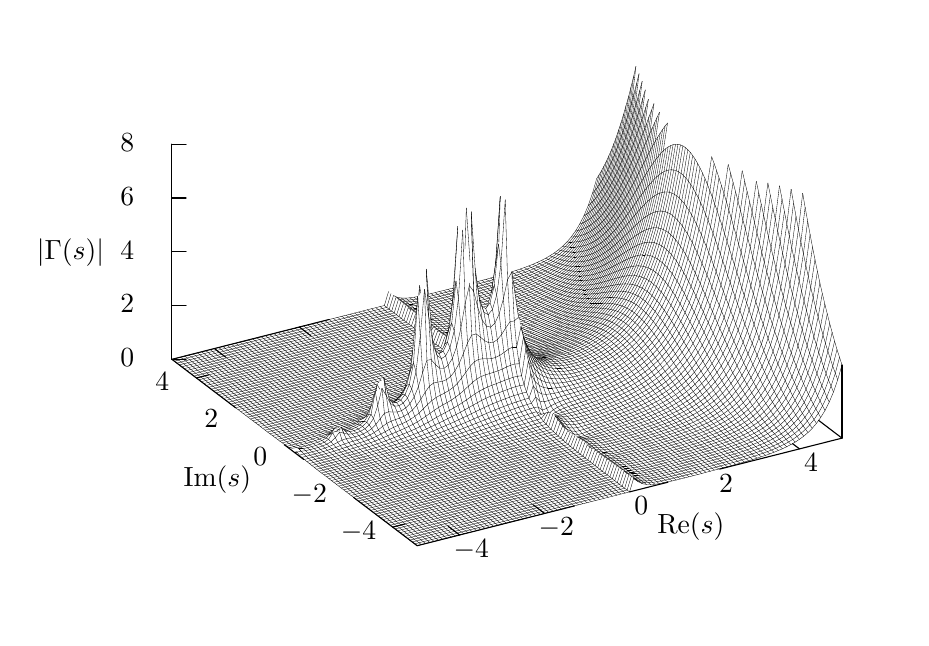
\begin{tikzpicture}[gnuplot]
%% generated with GNUPLOT 5.1p0 (Lua 5.3; terminal rev. 99, script rev. 100)
%% 水 11/21 05:26:31 2018
\path (0.000,0.000) rectangle (11.000,7.500);
\gpcolor{rgb color={0.000,0.000,0.000}}
\gpsetlinetype{gp lt border}
\gpsetdashtype{gp dt solid}
\gpsetlinewidth{0.30}
\draw[gp path] (6.492,4.572)--(6.438,4.544);
\draw[gp path] (6.469,4.528)--(6.438,4.544);
\draw[gp path] (6.384,4.519)--(6.438,4.544);
\draw[gp path] (6.546,4.603)--(6.492,4.572);
\draw[gp path] (6.523,4.558)--(6.492,4.572);
\draw[gp path] (6.415,4.502)--(6.384,4.519);
\draw[gp path] (6.330,4.495)--(6.384,4.519);
\draw[gp path] (6.577,4.590)--(6.546,4.603);
\draw[gp path] (6.600,4.638)--(6.546,4.603);
\draw[gp path] (6.276,4.474)--(6.330,4.495);
\draw[gp path] (6.362,4.477)--(6.330,4.495);
\draw[gp path] (6.222,4.454)--(6.276,4.474);
\draw[gp path] (6.308,4.455)--(6.276,4.474);
\draw[gp path] (6.654,4.678)--(6.600,4.638);
\draw[gp path] (6.631,4.628)--(6.600,4.638);
\draw[gp path] (6.254,4.434)--(6.222,4.454);
\draw[gp path] (6.169,4.435)--(6.222,4.454);
\draw[gp path] (6.685,4.670)--(6.654,4.678);
\draw[gp path] (6.708,4.725)--(6.654,4.678);
\draw[gp path] (6.200,4.415)--(6.169,4.435);
\draw[gp path] (6.115,4.417)--(6.169,4.435);
\draw[gp path] (6.501,4.513)--(6.469,4.528);
\draw[gp path] (6.523,4.558)--(6.469,4.528);
\draw[gp path] (6.415,4.502)--(6.469,4.528);
\draw[gp path] (6.362,4.477)--(6.415,4.502);
\draw[gp path] (6.447,4.485)--(6.415,4.502);
\draw[gp path] (6.555,4.544)--(6.523,4.558);
\draw[gp path] (6.577,4.590)--(6.523,4.558);
\draw[gp path] (6.308,4.455)--(6.362,4.477);
\draw[gp path] (6.393,4.460)--(6.362,4.477);
\draw[gp path] (6.146,4.396)--(6.115,4.417);
\draw[gp path] (6.061,4.400)--(6.115,4.417);
\draw[gp path] (6.608,4.579)--(6.577,4.590);
\draw[gp path] (6.631,4.628)--(6.577,4.590);
\draw[gp path] (6.254,4.434)--(6.308,4.455);
\draw[gp path] (6.339,4.437)--(6.308,4.455);
\draw[gp path] (6.739,4.719)--(6.708,4.725);
\draw[gp path] (6.762,4.778)--(6.708,4.725);
\draw[gp path] (6.285,4.415)--(6.254,4.434);
\draw[gp path] (6.092,4.378)--(6.062,4.399);
\draw[gp path] (6.200,4.415)--(6.254,4.434);
\draw[gp path] (6.662,4.618)--(6.631,4.628);
\draw[gp path] (6.685,4.670)--(6.631,4.628);
\draw[gp path] (6.146,4.396)--(6.200,4.415);
\draw[gp path] (6.231,4.395)--(6.200,4.415);
\draw[gp path] (6.478,4.469)--(6.447,4.485);
\draw[gp path] (6.393,4.460)--(6.447,4.485);
\draw[gp path] (6.501,4.513)--(6.447,4.485);
\draw[gp path] (6.092,4.378)--(6.146,4.396);
\draw[gp path] (6.177,4.376)--(6.146,4.396);
\draw[gp path] (6.555,4.544)--(6.501,4.513);
\draw[gp path] (6.532,4.499)--(6.501,4.513);
\draw[gp path] (6.739,4.719)--(6.685,4.670);
\draw[gp path] (6.716,4.663)--(6.685,4.670);
\draw[gp path] (6.424,4.443)--(6.393,4.460);
\draw[gp path] (6.339,4.437)--(6.393,4.460);
\draw[gp path] (6.586,4.531)--(6.555,4.544);
\draw[gp path] (6.608,4.579)--(6.555,4.544);
\draw[gp path] (6.285,4.415)--(6.339,4.437);
\draw[gp path] (6.370,4.419)--(6.339,4.437);
\draw[gp path] (6.793,4.776)--(6.762,4.778);
\draw[gp path] (6.816,4.841)--(6.762,4.778);
\draw[gp path] (6.066,4.370)--(6.092,4.378);
\draw[gp path] (6.123,4.357)--(6.092,4.378);
\draw[gp path] (6.640,4.568)--(6.608,4.579);
\draw[gp path] (6.662,4.618)--(6.608,4.579);
\draw[gp path] (6.316,4.396)--(6.285,4.415);
\draw[gp path] (6.231,4.395)--(6.285,4.415);
\draw[gp path] (6.262,4.375)--(6.231,4.395);
\draw[gp path] (6.177,4.376)--(6.231,4.395);
\draw[gp path] (6.770,4.715)--(6.739,4.719);
\draw[gp path] (6.793,4.776)--(6.739,4.719);
\draw[gp path] (6.694,4.609)--(6.662,4.618);
\draw[gp path] (6.716,4.663)--(6.662,4.618);
\draw[gp path] (6.208,4.355)--(6.177,4.376);
\draw[gp path] (6.123,4.357)--(6.177,4.376);
\draw[gp path] (5.792,4.320)--(5.831,4.331);
\draw[gp path] (6.424,4.443)--(6.478,4.469);
\draw[gp path] (6.509,4.454)--(6.478,4.469);
\draw[gp path] (6.532,4.499)--(6.478,4.469);
\draw[gp path] (6.455,4.426)--(6.424,4.443);
\draw[gp path] (6.370,4.419)--(6.424,4.443);
\draw[gp path] (6.563,4.485)--(6.532,4.499);
\draw[gp path] (6.586,4.531)--(6.532,4.499);
\draw[gp path] (6.401,4.401)--(6.370,4.419);
\draw[gp path] (6.316,4.396)--(6.370,4.419);
\draw[gp path] (6.070,4.340)--(6.123,4.357);
\draw[gp path] (6.154,4.337)--(6.123,4.357);
\draw[gp path] (6.640,4.568)--(6.586,4.531);
\draw[gp path] (6.617,4.519)--(6.586,4.531);
\draw[gp path] (6.262,4.375)--(6.316,4.396);
\draw[gp path] (6.347,4.378)--(6.316,4.396);
\draw[gp path] (6.770,4.715)--(6.716,4.663);
\draw[gp path] (6.748,4.657)--(6.716,4.663);
\draw[gp path] (5.823,4.298)--(5.792,4.320);
\draw[gp path] (5.738,4.305)--(5.792,4.320);
\draw[gp path] (6.847,4.843)--(6.816,4.841);
\draw[gp path] (6.870,4.916)--(6.816,4.841);
\draw[gp path] (6.100,4.319)--(6.070,4.339);
\draw[gp path] (6.293,4.356)--(6.262,4.375);
\draw[gp path] (6.208,4.355)--(6.262,4.375);
\draw[gp path] (6.671,4.558)--(6.640,4.568);
\draw[gp path] (6.694,4.609)--(6.640,4.568);
\draw[gp path] (6.847,4.843)--(6.793,4.776);
\draw[gp path] (6.824,4.776)--(6.793,4.776);
\draw[gp path] (5.769,4.283)--(5.738,4.305);
\draw[gp path] (5.684,4.291)--(5.738,4.305);
\draw[gp path] (5.823,4.298)--(5.826,4.299);
\draw[gp path] (6.239,4.336)--(6.208,4.355);
\draw[gp path] (6.154,4.337)--(6.208,4.355);
\draw[gp path] (6.725,4.602)--(6.694,4.609);
\draw[gp path] (6.748,4.657)--(6.694,4.609);
\draw[gp path] (6.185,4.316)--(6.154,4.337);
\draw[gp path] (6.100,4.319)--(6.154,4.337);
\draw[gp path] (6.486,4.411)--(6.455,4.426);
\draw[gp path] (6.401,4.401)--(6.455,4.426);
\draw[gp path] (6.509,4.454)--(6.455,4.426);
\draw[gp path] (6.540,4.440)--(6.509,4.454);
\draw[gp path] (6.563,4.485)--(6.509,4.454);
\draw[gp path] (6.432,4.384)--(6.401,4.401);
\draw[gp path] (6.347,4.378)--(6.401,4.401);
\draw[gp path] (6.801,4.712)--(6.770,4.715);
\draw[gp path] (6.824,4.776)--(6.770,4.715);
\draw[gp path] (5.769,4.283)--(5.823,4.298);
\draw[gp path] (5.825,4.296)--(5.823,4.298);
\draw[gp path] (5.715,4.268)--(5.684,4.291);
\draw[gp path] (5.630,4.276)--(5.684,4.291);
\draw[gp path] (6.594,4.472)--(6.563,4.485);
\draw[gp path] (6.617,4.519)--(6.563,4.485);
\draw[gp path] (6.293,4.356)--(6.347,4.378);
\draw[gp path] (6.378,4.360)--(6.347,4.378);
\draw[gp path] (6.075,4.311)--(6.100,4.319);
\draw[gp path] (6.131,4.298)--(6.100,4.319);
\draw[gp path] (6.648,4.508)--(6.617,4.519);
\draw[gp path] (6.671,4.558)--(6.617,4.519);
\draw[gp path] (6.239,4.336)--(6.293,4.356);
\draw[gp path] (6.324,4.337)--(6.293,4.356);
\draw[gp path] (5.800,4.260)--(5.769,4.283);
\draw[gp path] (5.715,4.268)--(5.769,4.283);
\draw[gp path] (5.620,4.273)--(5.630,4.276);
\draw[gp path] (5.661,4.253)--(5.630,4.276);
\draw[gp path] (6.185,4.316)--(6.239,4.336);
\draw[gp path] (6.270,4.316)--(6.239,4.336);
\draw[gp path] (6.779,4.653)--(6.748,4.657);
\draw[gp path] (6.801,4.712)--(6.748,4.657);
\draw[gp path] (6.725,4.602)--(6.671,4.558);
\draw[gp path] (6.702,4.549)--(6.671,4.558);
\draw[gp path] (6.216,4.296)--(6.185,4.316);
\draw[gp path] (6.131,4.298)--(6.185,4.316);
\draw[gp path] (6.901,4.923)--(6.870,4.916);
\draw[gp path] (6.924,5.005)--(6.870,4.916);
\draw[gp path] (5.661,4.253)--(5.715,4.268);
\draw[gp path] (5.746,4.245)--(5.715,4.268);
\draw[gp path] (5.800,4.260)--(5.821,4.266);
\draw[gp path] (6.878,4.847)--(6.847,4.843);
\draw[gp path] (6.901,4.923)--(6.847,4.843);
\draw[gp path] (6.517,4.396)--(6.486,4.411);
\draw[gp path] (6.432,4.384)--(6.486,4.411);
\draw[gp path] (6.540,4.440)--(6.486,4.411);
\draw[gp path] (6.378,4.360)--(6.432,4.384);
\draw[gp path] (6.463,4.368)--(6.432,4.384);
\draw[gp path] (6.571,4.426)--(6.540,4.440);
\draw[gp path] (6.594,4.472)--(6.540,4.440);
\draw[gp path] (6.324,4.337)--(6.378,4.360);
\draw[gp path] (6.409,4.343)--(6.378,4.360);
\draw[gp path] (6.079,4.281)--(6.131,4.298);
\draw[gp path] (6.162,4.277)--(6.131,4.298);
\draw[gp path] (6.878,4.847)--(6.824,4.776);
\draw[gp path] (6.855,4.777)--(6.824,4.776);
\draw[gp path] (6.625,4.460)--(6.594,4.472);
\draw[gp path] (6.648,4.508)--(6.594,4.472);
\draw[gp path] (6.779,4.653)--(6.725,4.602);
\draw[gp path] (6.756,4.596)--(6.725,4.602);
\draw[gp path] (5.818,4.247)--(5.800,4.260);
\draw[gp path] (5.746,4.245)--(5.800,4.260);
\draw[gp path] (5.692,4.230)--(5.661,4.253);
\draw[gp path] (5.624,4.243)--(5.661,4.253);
\draw[gp path] (6.270,4.316)--(6.324,4.337);
\draw[gp path] (6.355,4.319)--(6.324,4.337);
\draw[gp path] (6.108,4.259)--(6.079,4.279);
\draw[gp path] (6.216,4.296)--(6.270,4.316);
\draw[gp path] (6.301,4.297)--(6.270,4.316);
\draw[gp path] (6.833,4.712)--(6.801,4.712);
\draw[gp path] (6.679,4.499)--(6.648,4.508);
\draw[gp path] (6.702,4.549)--(6.648,4.508);
\draw[gp path] (6.855,4.777)--(6.801,4.712);
\draw[gp path] (5.777,4.222)--(5.746,4.245);
\draw[gp path] (5.692,4.230)--(5.746,4.245);
\draw[gp path] (5.638,4.216)--(5.627,4.224);
\draw[gp path] (6.248,4.277)--(6.216,4.296);
\draw[gp path] (6.162,4.277)--(6.216,4.296);
\draw[gp path] (6.756,4.596)--(6.702,4.549);
\draw[gp path] (6.733,4.542)--(6.702,4.549);
\draw[gp path] (6.194,4.257)--(6.162,4.277);
\draw[gp path] (6.810,4.650)--(6.779,4.653);
\draw[gp path] (6.833,4.712)--(6.779,4.653);
\draw[gp path] (6.108,4.259)--(6.162,4.277);
\draw[gp path] (6.517,4.396)--(6.463,4.368);
\draw[gp path] (6.409,4.343)--(6.463,4.368);
\draw[gp path] (6.494,4.352)--(6.463,4.368);
\draw[gp path] (6.571,4.426)--(6.517,4.396);
\draw[gp path] (6.548,4.381)--(6.517,4.396);
\draw[gp path] (5.638,4.216)--(5.692,4.230);
\draw[gp path] (5.723,4.207)--(5.692,4.230);
\draw[gp path] (5.777,4.222)--(5.816,4.233);
\draw[gp path] (6.355,4.319)--(6.409,4.343);
\draw[gp path] (6.441,4.326)--(6.409,4.343);
\draw[gp path] (6.625,4.460)--(6.571,4.426);
\draw[gp path] (6.602,4.414)--(6.571,4.426);
\draw[gp path] (6.301,4.297)--(6.355,4.319);
\draw[gp path] (6.387,4.301)--(6.355,4.319);
\draw[gp path] (6.083,4.251)--(6.108,4.259);
\draw[gp path] (6.140,4.239)--(6.108,4.259);
\draw[gp path] (6.656,4.450)--(6.625,4.460);
\draw[gp path] (6.679,4.499)--(6.625,4.460);
\draw[gp path] (6.248,4.277)--(6.301,4.297);
\draw[gp path] (6.333,4.279)--(6.301,4.297);
\draw[gp path] (5.809,4.200)--(5.777,4.222);
\draw[gp path] (5.723,4.207)--(5.777,4.222);
\draw[gp path] (5.629,4.213)--(5.638,4.216);
\draw[gp path] (5.669,4.193)--(5.638,4.216);
\draw[gp path] (6.909,4.853)--(6.878,4.847);
\draw[gp path] (6.932,4.931)--(6.878,4.847);
\draw[gp path] (6.810,4.650)--(6.756,4.596);
\draw[gp path] (6.787,4.591)--(6.756,4.596);
\draw[gp path] (6.955,5.017)--(6.901,4.923);
\draw[gp path] (6.932,4.931)--(6.901,4.923);
\draw[gp path] (5.306,4.191)--(5.320,4.195);
\draw[gp path] (6.194,4.257)--(6.248,4.277);
\draw[gp path] (6.279,4.257)--(6.248,4.277);
\draw[gp path] (6.887,4.780)--(6.855,4.777);
\draw[gp path] (6.909,4.853)--(6.855,4.777);
\draw[gp path] (6.710,4.490)--(6.679,4.499);
\draw[gp path] (6.733,4.542)--(6.679,4.499);
\draw[gp path] (6.955,5.017)--(6.924,5.005);
\draw[gp path] (6.978,5.111)--(6.924,5.005);
\draw[gp path] (5.755,4.185)--(5.723,4.207);
\draw[gp path] (5.669,4.193)--(5.723,4.207);
\draw[gp path] (5.809,4.200)--(5.812,4.201);
\draw[gp path] (6.140,4.239)--(6.194,4.257);
\draw[gp path] (6.225,4.237)--(6.194,4.257);
\draw[gp path] (6.864,4.712)--(6.833,4.712);
\draw[gp path] (6.887,4.780)--(6.833,4.712);
\draw[gp path] (5.319,4.181)--(5.306,4.191);
\draw[gp path] (5.252,4.177)--(5.306,4.191);
\draw[gp path] (6.548,4.381)--(6.494,4.352);
\draw[gp path] (6.441,4.326)--(6.494,4.352);
\draw[gp path] (6.526,4.337)--(6.494,4.352);
\draw[gp path] (6.387,4.301)--(6.441,4.326);
\draw[gp path] (6.472,4.310)--(6.441,4.326);
\draw[gp path] (6.602,4.414)--(6.548,4.381);
\draw[gp path] (6.580,4.368)--(6.548,4.381);
\draw[gp path] (6.171,4.218)--(6.140,4.239);
\draw[gp path] (6.088,4.222)--(6.140,4.239);
\draw[gp path] (6.418,4.284)--(6.387,4.301);
\draw[gp path] (6.333,4.279)--(6.387,4.301);
\draw[gp path] (6.787,4.591)--(6.733,4.542);
\draw[gp path] (6.764,4.536)--(6.733,4.542);
\draw[gp path] (5.811,4.198)--(5.809,4.200);
\draw[gp path] (5.755,4.185)--(5.809,4.200);
\draw[gp path] (5.633,4.183)--(5.669,4.193);
\draw[gp path] (5.701,4.170)--(5.669,4.193);
\draw[gp path] (6.634,4.402)--(6.602,4.414);
\draw[gp path] (6.656,4.450)--(6.602,4.414);
\draw[gp path] (6.364,4.261)--(6.333,4.279);
\draw[gp path] (6.279,4.257)--(6.333,4.279);
\draw[gp path] (6.864,4.712)--(6.810,4.650);
\draw[gp path] (6.841,4.649)--(6.810,4.650);
\draw[gp path] (5.198,4.163)--(5.252,4.177);
\draw[gp path] (5.283,4.154)--(5.252,4.177);
\draw[gp path] (6.117,4.200)--(6.088,4.219);
\draw[gp path] (6.310,4.239)--(6.279,4.257);
\draw[gp path] (6.225,4.237)--(6.279,4.257);
\draw[gp path] (6.710,4.490)--(6.656,4.450);
\draw[gp path] (6.687,4.440)--(6.656,4.450);
\draw[gp path] (5.701,4.170)--(5.755,4.185);
\draw[gp path] (5.786,4.162)--(5.755,4.185);
\draw[gp path] (5.647,4.155)--(5.635,4.163);
\draw[gp path] (6.256,4.218)--(6.225,4.237);
\draw[gp path] (6.171,4.218)--(6.225,4.237);
\draw[gp path] (5.283,4.154)--(5.318,4.163);
\draw[gp path] (5.229,4.141)--(5.198,4.163);
\draw[gp path] (5.144,4.150)--(5.198,4.163);
\draw[gp path] (6.818,4.588)--(6.787,4.591);
\draw[gp path] (6.841,4.649)--(6.787,4.591);
\draw[gp path] (6.741,4.482)--(6.710,4.490);
\draw[gp path] (6.764,4.536)--(6.710,4.490);
\draw[gp path] (6.202,4.198)--(6.171,4.218);
\draw[gp path] (6.117,4.200)--(6.171,4.218);
\draw[gp path] (5.647,4.155)--(5.701,4.170);
\draw[gp path] (5.732,4.148)--(5.701,4.170);
\draw[gp path] (5.786,4.162)--(5.807,4.168);
\draw[gp path] (6.503,4.294)--(6.472,4.310);
\draw[gp path] (6.526,4.337)--(6.472,4.310);
\draw[gp path] (6.418,4.284)--(6.472,4.310);
\draw[gp path] (6.580,4.368)--(6.526,4.337);
\draw[gp path] (6.557,4.323)--(6.526,4.337);
\draw[gp path] (6.364,4.261)--(6.418,4.284);
\draw[gp path] (6.449,4.268)--(6.418,4.284);
\draw[gp path] (6.611,4.355)--(6.580,4.368);
\draw[gp path] (6.634,4.402)--(6.580,4.368);
\draw[gp path] (5.229,4.141)--(5.283,4.154);
\draw[gp path] (5.315,4.131)--(5.283,4.154);
\draw[gp path] (6.310,4.239)--(6.364,4.261);
\draw[gp path] (6.395,4.243)--(6.364,4.261);
\draw[gp path] (6.963,4.943)--(6.909,4.853);
\draw[gp path] (6.941,4.861)--(6.909,4.853);
\draw[gp path] (5.090,4.136)--(5.144,4.150);
\draw[gp path] (6.092,4.192)--(6.117,4.200);
\draw[gp path] (6.148,4.180)--(6.117,4.200);
\draw[gp path] (5.176,4.127)--(5.144,4.150);
\draw[gp path] (6.918,4.785)--(6.887,4.780);
\draw[gp path] (6.941,4.861)--(6.887,4.780);
\draw[gp path] (6.986,5.032)--(6.932,4.931);
\draw[gp path] (6.963,4.943)--(6.932,4.931);
\draw[gp path] (6.687,4.440)--(6.634,4.402);
\draw[gp path] (6.665,4.391)--(6.634,4.402);
\draw[gp path] (6.256,4.218)--(6.310,4.239);
\draw[gp path] (6.341,4.220)--(6.310,4.239);
\draw[gp path] (5.732,4.148)--(5.786,4.162);
\draw[gp path] (5.804,4.150)--(5.786,4.162);
\draw[gp path] (5.678,4.133)--(5.647,4.155);
\draw[gp path] (5.637,4.154)--(5.647,4.155);
\draw[gp path] (6.918,4.785)--(6.864,4.712);
\draw[gp path] (6.895,4.715)--(6.864,4.712);
\draw[gp path] (6.795,4.531)--(6.764,4.536);
\draw[gp path] (6.818,4.588)--(6.764,4.536);
\draw[gp path] (5.315,4.131)--(5.316,4.132);
\draw[gp path] (6.287,4.199)--(6.256,4.218);
\draw[gp path] (6.202,4.198)--(6.256,4.218);
\draw[gp path] (5.176,4.127)--(5.229,4.141);
\draw[gp path] (5.261,4.117)--(5.229,4.141);
\draw[gp path] (6.986,5.032)--(6.955,5.017);
\draw[gp path] (7.009,5.130)--(6.955,5.017);
\draw[gp path] (5.036,4.123)--(5.090,4.136);
\draw[gp path] (6.719,4.431)--(6.687,4.440);
\draw[gp path] (5.122,4.113)--(5.090,4.136);
\draw[gp path] (6.741,4.482)--(6.687,4.440);
\draw[gp path] (5.763,4.126)--(5.732,4.148);
\draw[gp path] (5.678,4.133)--(5.732,4.148);
\draw[gp path] (6.148,4.180)--(6.202,4.198);
\draw[gp path] (6.233,4.179)--(6.202,4.198);
\draw[gp path] (6.895,4.715)--(6.841,4.649);
\draw[gp path] (6.872,4.649)--(6.841,4.649);
\draw[gp path] (5.261,4.117)--(5.315,4.131);
\draw[gp path] (5.316,4.130)--(5.315,4.131);
\draw[gp path] (5.207,4.104)--(5.176,4.127);
\draw[gp path] (5.122,4.113)--(5.176,4.127);
\draw[gp path] (6.534,4.280)--(6.503,4.294);
\draw[gp path] (6.449,4.268)--(6.503,4.294);
\draw[gp path] (6.557,4.323)--(6.503,4.294);
\draw[gp path] (6.480,4.252)--(6.449,4.268);
\draw[gp path] (6.395,4.243)--(6.449,4.268);
\draw[gp path] (6.588,4.310)--(6.557,4.323);
\draw[gp path] (6.611,4.355)--(6.557,4.323);
\draw[gp path] (6.096,4.162)--(6.148,4.180);
\draw[gp path] (6.179,4.159)--(6.148,4.180);
\draw[gp path] (5.068,4.100)--(5.036,4.123);
\draw[gp path] (5.004,4.115)--(5.036,4.123);
\draw[gp path] (6.426,4.226)--(6.395,4.243);
\draw[gp path] (6.341,4.220)--(6.395,4.243);
\draw[gp path] (5.641,4.123)--(5.678,4.133);
\draw[gp path] (5.709,4.111)--(5.678,4.133);
\draw[gp path] (6.773,4.476)--(6.741,4.482);
\draw[gp path] (6.795,4.531)--(6.741,4.482);
\draw[gp path] (5.763,4.126)--(5.802,4.137);
\draw[gp path] (6.665,4.391)--(6.611,4.355);
\draw[gp path] (6.642,4.344)--(6.611,4.355);
\draw[gp path] (6.287,4.199)--(6.341,4.220);
\draw[gp path] (6.872,4.649)--(6.818,4.588);
\draw[gp path] (6.849,4.587)--(6.818,4.588);
\draw[gp path] (6.372,4.202)--(6.341,4.220);
\draw[gp path] (7.009,5.130)--(6.978,5.111);
\draw[gp path] (7.032,5.240)--(6.978,5.111);
\draw[gp path] (5.292,4.094)--(5.261,4.117);
\draw[gp path] (5.207,4.104)--(5.261,4.117);
\draw[gp path] (6.125,4.142)--(6.097,4.160);
\draw[gp path] (5.068,4.100)--(5.122,4.113);
\draw[gp path] (5.153,4.090)--(5.122,4.113);
\draw[gp path] (6.318,4.180)--(6.287,4.199);
\draw[gp path] (6.233,4.179)--(6.287,4.199);
\draw[gp path] (6.719,4.431)--(6.665,4.391);
\draw[gp path] (6.696,4.381)--(6.665,4.391);
\draw[gp path] (5.793,4.104)--(5.763,4.126);
\draw[gp path] (5.709,4.111)--(5.763,4.126);
\draw[gp path] (5.655,4.096)--(5.644,4.104);
\draw[gp path] (5.014,4.087)--(5.006,4.093);
\draw[gp path] (5.292,4.094)--(5.314,4.100);
\draw[gp path] (6.264,4.159)--(6.233,4.179);
\draw[gp path] (6.179,4.159)--(6.233,4.179);
\draw[gp path] (5.238,4.080)--(5.207,4.104);
\draw[gp path] (5.153,4.090)--(5.207,4.104);
\draw[gp path] (6.827,4.528)--(6.795,4.531);
\draw[gp path] (6.849,4.587)--(6.795,4.531);
\draw[gp path] (5.014,4.087)--(5.068,4.100);
\draw[gp path] (5.099,4.077)--(5.068,4.100);
\draw[gp path] (6.773,4.476)--(6.719,4.431);
\draw[gp path] (6.750,4.423)--(6.719,4.431);
\draw[gp path] (6.972,4.871)--(6.918,4.785);
\draw[gp path] (6.949,4.792)--(6.918,4.785);
\draw[gp path] (5.740,4.088)--(5.709,4.111);
\draw[gp path] (5.655,4.096)--(5.709,4.111);
\draw[gp path] (6.210,4.141)--(6.179,4.159);
\draw[gp path] (6.972,4.871)--(6.941,4.861);
\draw[gp path] (6.995,4.956)--(6.941,4.861);
\draw[gp path] (6.125,4.142)--(6.179,4.159);
\draw[gp path] (6.511,4.236)--(6.480,4.252);
\draw[gp path] (6.534,4.280)--(6.480,4.252);
\draw[gp path] (6.426,4.226)--(6.480,4.252);
\draw[gp path] (6.949,4.792)--(6.895,4.715);
\draw[gp path] (6.926,4.719)--(6.895,4.715);
\draw[gp path] (6.588,4.310)--(6.534,4.280);
\draw[gp path] (6.565,4.266)--(6.534,4.280);
\draw[gp path] (6.372,4.202)--(6.426,4.226);
\draw[gp path] (6.457,4.210)--(6.426,4.226);
\draw[gp path] (5.238,4.080)--(5.292,4.094);
\draw[gp path] (5.312,4.079)--(5.292,4.094);
\draw[gp path] (6.642,4.344)--(6.588,4.310);
\draw[gp path] (6.619,4.298)--(6.588,4.310);
\draw[gp path] (6.995,4.956)--(6.963,4.943);
\draw[gp path] (7.017,5.050)--(6.963,4.943);
\draw[gp path] (5.099,4.077)--(5.153,4.090);
\draw[gp path] (5.184,4.067)--(5.153,4.090);
\draw[gp path] (6.403,4.185)--(6.372,4.202);
\draw[gp path] (6.318,4.180)--(6.372,4.202);
\draw[gp path] (6.101,4.134)--(6.125,4.142);
\draw[gp path] (6.156,4.122)--(6.125,4.142);
\draw[gp path] (5.740,4.088)--(5.792,4.103);
\draw[gp path] (5.645,4.093)--(5.655,4.096);
\draw[gp path] (6.903,4.651)--(6.872,4.649);
\draw[gp path] (6.926,4.719)--(6.872,4.649);
\draw[gp path] (5.686,4.073)--(5.655,4.096);
\draw[gp path] (5.006,4.085)--(5.014,4.087);
\draw[gp path] (5.045,4.064)--(5.014,4.087);
\draw[gp path] (6.696,4.381)--(6.642,4.344);
\draw[gp path] (6.673,4.333)--(6.642,4.344);
\draw[gp path] (6.264,4.159)--(6.318,4.180);
\draw[gp path] (6.349,4.162)--(6.318,4.180);
\draw[gp path] (6.827,4.528)--(6.773,4.476);
\draw[gp path] (6.804,4.471)--(6.773,4.476);
\draw[gp path] (5.269,4.057)--(5.238,4.080);
\draw[gp path] (5.184,4.067)--(5.238,4.080);
\draw[gp path] (4.821,4.077)--(4.867,4.085);
\draw[gp path] (6.295,4.141)--(6.264,4.159);
\draw[gp path] (6.210,4.141)--(6.264,4.159);
\draw[gp path] (7.017,5.050)--(6.986,5.032);
\draw[gp path] (7.040,5.152)--(6.986,5.032);
\draw[gp path] (5.130,4.053)--(5.099,4.077);
\draw[gp path] (5.045,4.064)--(5.099,4.077);
\draw[gp path] (6.750,4.423)--(6.696,4.381);
\draw[gp path] (6.727,4.373)--(6.696,4.381);
\draw[gp path] (5.686,4.073)--(5.740,4.088);
\draw[gp path] (5.771,4.066)--(5.740,4.088);
\draw[gp path] (6.880,4.587)--(6.849,4.587);
\draw[gp path] (6.903,4.651)--(6.849,4.587);
\draw[gp path] (6.156,4.122)--(6.210,4.141);
\draw[gp path] (6.241,4.121)--(6.210,4.141);
\draw[gp path] (5.269,4.057)--(5.311,4.068);
\draw[gp path] (5.130,4.053)--(5.184,4.067);
\draw[gp path] (5.215,4.043)--(5.184,4.067);
\draw[gp path] (6.457,4.210)--(6.511,4.236);
\draw[gp path] (6.565,4.266)--(6.511,4.236);
\draw[gp path] (6.542,4.222)--(6.511,4.236);
\draw[gp path] (6.403,4.185)--(6.457,4.210);
\draw[gp path] (6.488,4.194)--(6.457,4.210);
\draw[gp path] (6.187,4.102)--(6.156,4.122);
\draw[gp path] (6.105,4.104)--(6.156,4.122);
\draw[gp path] (5.009,4.056)--(5.045,4.064);
\draw[gp path] (5.076,4.040)--(5.045,4.064);
\draw[gp path] (5.717,4.050)--(5.686,4.073);
\draw[gp path] (5.651,4.064)--(5.686,4.073);
\draw[gp path] (6.596,4.252)--(6.565,4.266);
\draw[gp path] (6.619,4.298)--(6.565,4.266);
\draw[gp path] (4.767,4.069)--(4.821,4.077);
\draw[gp path] (4.852,4.053)--(4.821,4.077);
\draw[gp path] (5.771,4.066)--(5.782,4.069);
\draw[gp path] (6.804,4.471)--(6.750,4.423);
\draw[gp path] (6.781,4.417)--(6.750,4.423);
\draw[gp path] (6.434,4.168)--(6.403,4.185);
\draw[gp path] (6.349,4.162)--(6.403,4.185);
\draw[gp path] (6.858,4.526)--(6.827,4.528);
\draw[gp path] (6.880,4.587)--(6.827,4.528);
\draw[gp path] (6.673,4.333)--(6.619,4.298);
\draw[gp path] (6.650,4.286)--(6.619,4.298);
\draw[gp path] (5.215,4.043)--(5.269,4.057);
\draw[gp path] (5.300,4.034)--(5.269,4.057);
\draw[gp path] (6.380,4.145)--(6.349,4.162);
\draw[gp path] (6.295,4.141)--(6.349,4.162);
\draw[gp path] (4.852,4.053)--(4.865,4.056);
\draw[gp path] (6.133,4.083)--(6.106,4.101);
\draw[gp path] (7.040,5.152)--(7.009,5.130);
\draw[gp path] (7.063,5.267)--(7.009,5.130);
\draw[gp path] (5.161,4.030)--(5.130,4.053);
\draw[gp path] (5.076,4.040)--(5.130,4.053);
\draw[gp path] (6.241,4.121)--(6.295,4.141);
\draw[gp path] (6.326,4.123)--(6.295,4.141);
\draw[gp path] (5.717,4.050)--(5.771,4.066);
\draw[gp path] (5.780,4.059)--(5.771,4.066);
\draw[gp path] (5.663,4.036)--(5.659,4.039);
\draw[gp path] (6.727,4.373)--(6.673,4.333);
\draw[gp path] (6.704,4.323)--(6.673,4.333);
\draw[gp path] (5.022,4.028)--(5.011,4.036);
\draw[gp path] (5.300,4.034)--(5.309,4.036);
\draw[gp path] (7.003,4.884)--(6.949,4.792);
\draw[gp path] (6.980,4.802)--(6.949,4.792);
\draw[gp path] (6.957,4.726)--(6.926,4.719);
\draw[gp path] (6.980,4.802)--(6.926,4.719);
\draw[gp path] (6.273,4.102)--(6.241,4.121);
\draw[gp path] (6.187,4.102)--(6.241,4.121);
\draw[gp path] (5.246,4.020)--(5.215,4.043);
\draw[gp path] (5.161,4.030)--(5.215,4.043);
\draw[gp path] (4.798,4.045)--(4.767,4.069);
\draw[gp path] (4.713,4.065)--(4.767,4.069);
\draw[gp path] (7.026,4.973)--(6.972,4.871);
\draw[gp path] (7.003,4.884)--(6.972,4.871);
\draw[gp path] (6.858,4.526)--(6.804,4.471);
\draw[gp path] (6.835,4.468)--(6.804,4.471);
\draw[gp path] (5.107,4.017)--(5.076,4.040);
\draw[gp path] (5.022,4.028)--(5.076,4.040);
\draw[gp path] (4.864,4.044)--(4.852,4.053);
\draw[gp path] (4.798,4.045)--(4.852,4.053);
\draw[gp path] (5.748,4.028)--(5.717,4.050);
\draw[gp path] (5.663,4.036)--(5.717,4.050);
\draw[gp path] (6.957,4.726)--(6.903,4.651);
\draw[gp path] (6.934,4.655)--(6.903,4.651);
\draw[gp path] (6.758,4.365)--(6.727,4.373);
\draw[gp path] (6.781,4.417)--(6.727,4.373);
\draw[gp path] (6.219,4.082)--(6.187,4.102);
\draw[gp path] (6.133,4.083)--(6.187,4.102);
\draw[gp path] (5.308,4.027)--(5.300,4.034);
\draw[gp path] (5.246,4.020)--(5.300,4.034);
\draw[gp path] (6.542,4.222)--(6.488,4.194);
\draw[gp path] (6.434,4.168)--(6.488,4.194);
\draw[gp path] (6.520,4.179)--(6.488,4.194);
\draw[gp path] (6.573,4.208)--(6.542,4.222);
\draw[gp path] (6.596,4.252)--(6.542,4.222);
\draw[gp path] (7.048,5.070)--(6.995,4.956);
\draw[gp path] (7.026,4.973)--(6.995,4.956);
\draw[gp path] (6.466,4.153)--(6.434,4.168);
\draw[gp path] (6.380,4.145)--(6.434,4.168);
\draw[gp path] (5.192,4.006)--(5.161,4.030);
\draw[gp path] (5.107,4.017)--(5.161,4.030);
\draw[gp path] (6.627,4.240)--(6.596,4.252);
\draw[gp path] (6.650,4.286)--(6.596,4.252);
\draw[gp path] (6.912,4.588)--(6.880,4.587);
\draw[gp path] (6.934,4.655)--(6.880,4.587);
\draw[gp path] (6.109,4.075)--(6.133,4.083);
\draw[gp path] (6.165,4.063)--(6.133,4.083);
\draw[gp path] (6.412,4.128)--(6.380,4.145);
\draw[gp path] (6.326,4.123)--(6.380,4.145);
\draw[gp path] (5.660,4.035)--(5.663,4.036);
\draw[gp path] (5.695,4.013)--(5.663,4.036);
\draw[gp path] (5.748,4.028)--(5.773,4.035);
\draw[gp path] (5.053,4.004)--(5.022,4.028);
\draw[gp path] (5.012,4.026)--(5.022,4.028);
\draw[gp path] (6.704,4.323)--(6.650,4.286);
\draw[gp path] (6.681,4.275)--(6.650,4.286);
\draw[gp path] (6.273,4.102)--(6.326,4.123);
\draw[gp path] (6.358,4.105)--(6.326,4.123);
\draw[gp path] (6.835,4.468)--(6.781,4.417);
\draw[gp path] (6.812,4.412)--(6.781,4.417);
\draw[gp path] (4.744,4.041)--(4.713,4.065);
\draw[gp path] (4.659,4.066)--(4.713,4.065);
\draw[gp path] (7.086,5.395)--(7.032,5.240);
\draw[gp path] (7.063,5.267)--(7.032,5.240);
\draw[gp path] (5.192,4.006)--(5.246,4.020);
\draw[gp path] (5.277,3.996)--(5.246,4.020);
\draw[gp path] (4.829,4.022)--(4.798,4.045);
\draw[gp path] (4.744,4.041)--(4.798,4.045);
\draw[gp path] (6.304,4.084)--(6.273,4.102);
\draw[gp path] (6.219,4.082)--(6.273,4.102);
\draw[gp path] (5.138,3.993)--(5.107,4.017);
\draw[gp path] (5.053,4.004)--(5.107,4.017);
\draw[gp path] (4.829,4.022)--(4.862,4.026);
\draw[gp path] (6.889,4.525)--(6.858,4.526);
\draw[gp path] (6.912,4.588)--(6.858,4.526);
\draw[gp path] (5.695,4.013)--(5.748,4.028);
\draw[gp path] (5.767,4.015)--(5.748,4.028);
\draw[gp path] (7.048,5.070)--(7.017,5.050);
\draw[gp path] (7.071,5.178)--(7.017,5.050);
\draw[gp path] (6.758,4.365)--(6.704,4.323);
\draw[gp path] (6.735,4.315)--(6.704,4.323);
\draw[gp path] (5.277,3.996)--(5.306,4.003);
\draw[gp path] (6.165,4.063)--(6.219,4.082);
\draw[gp path] (6.250,4.063)--(6.219,4.082);
\draw[gp path] (5.138,3.993)--(5.192,4.006);
\draw[gp path] (5.223,3.982)--(5.192,4.006);
\draw[gp path] (5.726,3.990)--(5.695,4.013);
\draw[gp path] (5.669,4.006)--(5.695,4.013);
\draw[gp path] (5.084,3.980)--(5.053,4.004);
\draw[gp path] (5.014,3.996)--(5.053,4.004);
\draw[gp path] (6.114,4.046)--(6.165,4.063);
\draw[gp path] (6.196,4.043)--(6.165,4.063);
\draw[gp path] (6.466,4.153)--(6.520,4.179);
\draw[gp path] (6.551,4.165)--(6.520,4.179);
\draw[gp path] (6.573,4.208)--(6.520,4.179);
\draw[gp path] (6.497,4.138)--(6.466,4.153);
\draw[gp path] (6.412,4.128)--(6.466,4.153);
\draw[gp path] (6.605,4.195)--(6.573,4.208);
\draw[gp path] (6.627,4.240)--(6.573,4.208);
\draw[gp path] (6.789,4.359)--(6.758,4.365);
\draw[gp path] (6.812,4.412)--(6.758,4.365);
\draw[gp path] (6.889,4.525)--(6.835,4.468);
\draw[gp path] (6.866,4.465)--(6.835,4.468);
\draw[gp path] (6.443,4.112)--(6.412,4.128);
\draw[gp path] (6.358,4.105)--(6.412,4.128);
\draw[gp path] (4.775,4.017)--(4.744,4.041);
\draw[gp path] (4.690,4.042)--(4.744,4.041);
\draw[gp path] (5.302,3.977)--(5.277,3.996);
\draw[gp path] (5.223,3.982)--(5.277,3.996);
\draw[gp path] (4.775,4.017)--(4.829,4.022);
\draw[gp path] (4.859,3.998)--(4.829,4.022);
\draw[gp path] (6.659,4.229)--(6.627,4.240);
\draw[gp path] (6.681,4.275)--(6.627,4.240);
\draw[gp path] (6.304,4.084)--(6.358,4.105);
\draw[gp path] (6.389,4.088)--(6.358,4.105);
\draw[gp path] (5.169,3.969)--(5.138,3.993);
\draw[gp path] (5.084,3.980)--(5.138,3.993);
\draw[gp path] (6.142,4.025)--(6.114,4.042);
\draw[gp path] (4.690,4.042)--(4.659,4.066);
\draw[gp path] (4.605,4.077)--(4.659,4.066);
\draw[gp path] (6.988,4.734)--(6.957,4.726);
\draw[gp path] (7.011,4.813)--(6.957,4.726);
\draw[gp path] (7.011,4.813)--(6.980,4.802);
\draw[gp path] (7.034,4.899)--(6.980,4.802);
\draw[gp path] (5.726,3.990)--(5.763,4.001);
\draw[gp path] (6.250,4.063)--(6.304,4.084);
\draw[gp path] (6.335,4.065)--(6.304,4.084);
\draw[gp path] (6.988,4.734)--(6.934,4.655);
\draw[gp path] (6.966,4.661)--(6.934,4.655);
\draw[gp path] (6.735,4.315)--(6.681,4.275);
\draw[gp path] (6.713,4.266)--(6.681,4.275);
\draw[gp path] (5.030,3.968)--(5.016,3.979);
\draw[gp path] (7.094,5.297)--(7.040,5.152);
\draw[gp path] (7.071,5.178)--(7.040,5.152);
\draw[gp path] (5.255,3.958)--(5.223,3.982);
\draw[gp path] (5.169,3.969)--(5.223,3.982);
\draw[gp path] (7.057,4.992)--(7.003,4.884);
\draw[gp path] (7.034,4.899)--(7.003,4.884);
\draw[gp path] (6.196,4.043)--(6.250,4.063);
\draw[gp path] (6.281,4.044)--(6.250,4.063);
\draw[gp path] (6.943,4.592)--(6.912,4.588);
\draw[gp path] (6.966,4.661)--(6.912,4.588);
\draw[gp path] (6.866,4.465)--(6.812,4.412);
\draw[gp path] (6.843,4.408)--(6.812,4.412);
\draw[gp path] (5.030,3.968)--(5.084,3.980);
\draw[gp path] (5.115,3.956)--(5.084,3.980);
\draw[gp path] (4.474,3.948)--(4.443,3.971);
\draw[gp path] (4.497,4.150)--(4.443,3.971);
\draw[gp path] (4.389,3.958)--(4.443,3.971);
\draw[gp path] (5.679,3.977)--(5.726,3.990);
\draw[gp path] (5.754,3.970)--(5.726,3.990);
\draw[gp path] (6.766,4.307)--(6.735,4.315);
\draw[gp path] (6.789,4.359)--(6.735,4.315);
\draw[gp path] (4.721,4.018)--(4.775,4.017);
\draw[gp path] (4.806,3.993)--(4.775,4.017);
\draw[gp path] (6.142,4.025)--(6.196,4.043);
\draw[gp path] (6.227,4.024)--(6.196,4.043);
\draw[gp path] (4.806,3.993)--(4.859,3.998);
\draw[gp path] (5.255,3.958)--(5.301,3.970);
\draw[gp path] (5.115,3.956)--(5.169,3.969);
\draw[gp path] (5.201,3.944)--(5.169,3.969);
\draw[gp path] (4.636,4.052)--(4.690,4.042);
\draw[gp path] (4.721,4.018)--(4.690,4.042);
\draw[gp path] (7.080,5.094)--(7.026,4.973);
\draw[gp path] (7.057,4.992)--(7.026,4.973);
\draw[gp path] (6.528,4.123)--(6.497,4.138);
\draw[gp path] (6.551,4.165)--(6.497,4.138);
\draw[gp path] (6.443,4.112)--(6.497,4.138);
\draw[gp path] (6.943,4.592)--(6.889,4.525);
\draw[gp path] (6.920,4.526)--(6.889,4.525);
\draw[gp path] (6.605,4.195)--(6.551,4.165);
\draw[gp path] (6.582,4.152)--(6.551,4.165);
\draw[gp path] (6.474,4.096)--(6.443,4.112);
\draw[gp path] (6.389,4.088)--(6.443,4.112);
\draw[gp path] (6.118,4.017)--(6.142,4.025);
\draw[gp path] (6.173,4.005)--(6.142,4.025);
\draw[gp path] (6.636,4.183)--(6.605,4.195);
\draw[gp path] (6.659,4.229)--(6.605,4.195);
\draw[gp path] (4.335,3.944)--(4.389,3.958);
\draw[gp path] (4.420,3.934)--(4.389,3.958);
\draw[gp path] (6.335,4.065)--(6.389,4.088);
\draw[gp path] (6.420,4.071)--(6.389,4.088);
\draw[gp path] (5.062,3.944)--(5.030,3.968);
\draw[gp path] (5.017,3.966)--(5.030,3.968);
\draw[gp path] (5.286,3.934)--(5.255,3.958);
\draw[gp path] (5.201,3.944)--(5.255,3.958);
\draw[gp path] (6.366,4.048)--(6.335,4.065);
\draw[gp path] (6.281,4.044)--(6.335,4.065);
\draw[gp path] (6.690,4.218)--(6.659,4.229);
\draw[gp path] (6.713,4.266)--(6.659,4.229);
\draw[gp path] (6.843,4.408)--(6.789,4.359);
\draw[gp path] (6.820,4.353)--(6.789,4.359);
\draw[gp path] (5.062,3.944)--(5.115,3.956);
\draw[gp path] (5.147,3.931)--(5.115,3.956);
\draw[gp path] (4.559,4.098)--(4.605,4.077);
\draw[gp path] (4.636,4.052)--(4.605,4.077);
\draw[gp path] (4.528,4.124)--(4.474,3.948);
\draw[gp path] (4.420,3.934)--(4.474,3.948);
\draw[gp path] (4.505,3.924)--(4.474,3.948);
\draw[gp path] (6.920,4.526)--(6.866,4.465);
\draw[gp path] (6.897,4.465)--(6.866,4.465);
\draw[gp path] (6.312,4.026)--(6.281,4.044);
\draw[gp path] (6.227,4.024)--(6.281,4.044);
\draw[gp path] (5.703,3.953)--(5.751,3.966);
\draw[gp path] (4.752,3.993)--(4.806,3.993);
\draw[gp path] (4.837,3.968)--(4.806,3.993);
\draw[gp path] (4.837,3.968)--(4.857,3.970);
\draw[gp path] (4.281,3.931)--(4.335,3.944);
\draw[gp path] (4.366,3.920)--(4.335,3.944);
\draw[gp path] (5.286,3.934)--(5.296,3.937);
\draw[gp path] (6.744,4.257)--(6.713,4.266);
\draw[gp path] (6.766,4.307)--(6.713,4.266);
\draw[gp path] (5.232,3.919)--(5.201,3.944);
\draw[gp path] (5.147,3.931)--(5.201,3.944);
\draw[gp path] (7.117,5.432)--(7.063,5.267);
\draw[gp path] (7.094,5.297)--(7.063,5.267);
\draw[gp path] (7.080,5.094)--(7.048,5.070);
\draw[gp path] (7.102,5.206)--(7.048,5.070);
\draw[gp path] (4.752,3.993)--(4.721,4.018);
\draw[gp path] (4.667,4.027)--(4.721,4.018);
\draw[gp path] (6.258,4.005)--(6.227,4.024);
\draw[gp path] (6.173,4.005)--(6.227,4.024);
\draw[gp path] (4.366,3.920)--(4.420,3.934);
\draw[gp path] (4.451,3.910)--(4.420,3.934);
\draw[gp path] (5.093,3.919)--(5.062,3.944);
\draw[gp path] (5.020,3.935)--(5.062,3.944);
\draw[gp path] (6.122,3.987)--(6.173,4.005);
\draw[gp path] (6.204,3.985)--(6.173,4.005);
\draw[gp path] (5.295,3.927)--(5.286,3.934);
\draw[gp path] (5.232,3.919)--(5.286,3.934);
\draw[gp path] (4.227,3.917)--(4.281,3.931);
\draw[gp path] (4.312,3.907)--(4.281,3.931);
\draw[gp path] (6.582,4.152)--(6.528,4.123);
\draw[gp path] (6.559,4.109)--(6.528,4.123);
\draw[gp path] (6.474,4.096)--(6.528,4.123);
\draw[gp path] (7.042,4.827)--(6.988,4.734);
\draw[gp path] (6.897,4.465)--(6.843,4.408);
\draw[gp path] (7.020,4.745)--(6.988,4.734);
\draw[gp path] (6.874,4.406)--(6.843,4.408);
\draw[gp path] (6.420,4.071)--(6.474,4.096);
\draw[gp path] (6.505,4.081)--(6.474,4.096);
\draw[gp path] (6.798,4.301)--(6.766,4.307);
\draw[gp path] (6.820,4.353)--(6.766,4.307);
\draw[gp path] (6.997,4.668)--(6.966,4.661);
\draw[gp path] (7.020,4.745)--(6.966,4.661);
\draw[gp path] (6.636,4.183)--(6.582,4.152);
\draw[gp path] (6.613,4.140)--(6.582,4.152);
\draw[gp path] (6.366,4.048)--(6.420,4.071);
\draw[gp path] (6.451,4.055)--(6.420,4.071);
\draw[gp path] (5.093,3.919)--(5.147,3.931);
\draw[gp path] (5.178,3.906)--(5.147,3.931);
\draw[gp path] (4.667,4.027)--(4.636,4.052);
\draw[gp path] (4.591,4.073)--(4.636,4.052);
\draw[gp path] (7.065,4.916)--(7.011,4.813);
\draw[gp path] (7.042,4.827)--(7.011,4.813);
\draw[gp path] (4.559,4.098)--(4.505,3.924);
\draw[gp path] (4.536,3.900)--(4.505,3.924);
\draw[gp path] (4.451,3.910)--(4.505,3.924);
\draw[gp path] (6.667,4.172)--(6.636,4.183);
\draw[gp path] (6.690,4.218)--(6.636,4.183);
\draw[gp path] (6.974,4.597)--(6.943,4.592);
\draw[gp path] (6.997,4.668)--(6.943,4.592);
\draw[gp path] (6.397,4.031)--(6.366,4.048);
\draw[gp path] (6.312,4.026)--(6.366,4.048);
\draw[gp path] (6.150,3.966)--(6.123,3.984);
\draw[gp path] (4.855,3.954)--(4.837,3.968);
\draw[gp path] (4.783,3.969)--(4.837,3.968);
\draw[gp path] (4.312,3.907)--(4.366,3.920);
\draw[gp path] (4.397,3.897)--(4.366,3.920);
\draw[gp path] (5.178,3.906)--(5.232,3.919);
\draw[gp path] (5.263,3.896)--(5.232,3.919);
\draw[gp path] (6.343,4.008)--(6.312,4.026);
\draw[gp path] (6.258,4.005)--(6.312,4.026);
\draw[gp path] (5.039,3.908)--(5.021,3.922);
\draw[gp path] (4.698,4.003)--(4.752,3.993);
\draw[gp path] (4.783,3.969)--(4.752,3.993);
\draw[gp path] (4.173,3.903)--(4.227,3.917);
\draw[gp path] (4.258,3.893)--(4.227,3.917);
\draw[gp path] (6.721,4.209)--(6.690,4.218);
\draw[gp path] (6.744,4.257)--(6.690,4.218);
\draw[gp path] (7.065,4.916)--(7.034,4.899);
\draw[gp path] (7.088,5.014)--(7.034,4.899);
\draw[gp path] (6.951,4.529)--(6.920,4.526);
\draw[gp path] (6.974,4.597)--(6.920,4.526);
\draw[gp path] (5.039,3.908)--(5.093,3.919);
\draw[gp path] (5.124,3.895)--(5.093,3.919);
\draw[gp path] (6.204,3.985)--(6.258,4.005);
\draw[gp path] (6.289,3.987)--(6.258,4.005);
\draw[gp path] (4.482,3.887)--(4.451,3.910);
\draw[gp path] (4.397,3.897)--(4.451,3.910);
\draw[gp path] (6.874,4.406)--(6.820,4.353);
\draw[gp path] (6.852,4.350)--(6.820,4.353);
\draw[gp path] (7.125,5.332)--(7.071,5.178);
\draw[gp path] (7.102,5.206)--(7.071,5.178);
\draw[gp path] (4.343,3.883)--(4.312,3.907);
\draw[gp path] (4.258,3.893)--(4.312,3.907);
\draw[gp path] (5.263,3.896)--(5.291,3.904);
\draw[gp path] (5.209,3.883)--(5.178,3.906);
\draw[gp path] (5.124,3.895)--(5.178,3.906);
\draw[gp path] (6.775,4.250)--(6.744,4.257);
\draw[gp path] (6.798,4.301)--(6.744,4.257);
\draw[gp path] (6.235,3.966)--(6.204,3.985);
\draw[gp path] (6.150,3.966)--(6.204,3.985);
\draw[gp path] (4.119,3.889)--(4.173,3.903);
\draw[gp path] (4.204,3.879)--(4.173,3.903);
\draw[gp path] (4.623,4.047)--(4.667,4.027);
\draw[gp path] (4.698,4.003)--(4.667,4.027);
\draw[gp path] (6.951,4.529)--(6.897,4.465);
\draw[gp path] (6.928,4.465)--(6.897,4.465);
\draw[gp path] (4.568,3.877)--(4.536,3.900);
\draw[gp path] (4.482,3.887)--(4.536,3.900);
\draw[gp path] (4.590,4.071)--(4.536,3.900);
\draw[gp path] (4.815,3.944)--(4.854,3.944);
\draw[gp path] (6.451,4.055)--(6.505,4.081);
\draw[gp path] (6.559,4.109)--(6.505,4.081);
\draw[gp path] (6.536,4.067)--(6.505,4.081);
\draw[gp path] (4.343,3.883)--(4.397,3.897);
\draw[gp path] (4.429,3.873)--(4.397,3.897);
\draw[gp path] (6.613,4.140)--(6.559,4.109);
\draw[gp path] (6.590,4.096)--(6.559,4.109);
\draw[gp path] (7.111,5.120)--(7.057,4.992);
\draw[gp path] (7.088,5.014)--(7.057,4.992);
\draw[gp path] (6.482,4.040)--(6.451,4.055);
\draw[gp path] (6.397,4.031)--(6.451,4.055);
\draw[gp path] (6.127,3.958)--(6.150,3.966);
\draw[gp path] (6.181,3.947)--(6.150,3.966);
\draw[gp path] (5.022,3.906)--(5.039,3.908);
\draw[gp path] (5.070,3.884)--(5.039,3.908);
\draw[gp path] (4.815,3.944)--(4.783,3.969);
\draw[gp path] (4.729,3.978)--(4.783,3.969);
\draw[gp path] (5.287,3.879)--(5.263,3.896);
\draw[gp path] (5.209,3.883)--(5.263,3.896);
\draw[gp path] (6.667,4.172)--(6.613,4.140);
\draw[gp path] (6.644,4.128)--(6.613,4.140);
\draw[gp path] (4.289,3.869)--(4.258,3.893);
\draw[gp path] (4.204,3.879)--(4.258,3.893);
\draw[gp path] (6.428,4.014)--(6.397,4.031);
\draw[gp path] (6.343,4.008)--(6.397,4.031);
\draw[gp path] (4.065,3.876)--(4.119,3.889);
\draw[gp path] (4.150,3.866)--(4.119,3.889);
\draw[gp path] (5.070,3.884)--(5.124,3.895);
\draw[gp path] (5.155,3.871)--(5.124,3.895);
\draw[gp path] (6.289,3.987)--(6.343,4.008);
\draw[gp path] (6.374,3.991)--(6.343,4.008);
\draw[gp path] (6.852,4.350)--(6.798,4.301);
\draw[gp path] (6.829,4.295)--(6.798,4.301);
\draw[gp path] (6.721,4.209)--(6.667,4.172);
\draw[gp path] (6.698,4.162)--(6.667,4.172);
\draw[gp path] (4.429,3.873)--(4.482,3.887);
\draw[gp path] (4.514,3.863)--(4.482,3.887);
\draw[gp path] (7.140,5.584)--(7.086,5.395);
\draw[gp path] (7.117,5.432)--(7.086,5.395);
\draw[gp path] (6.906,4.405)--(6.874,4.406);
\draw[gp path] (6.928,4.465)--(6.874,4.406);
\draw[gp path] (4.289,3.869)--(4.343,3.883);
\draw[gp path] (4.375,3.859)--(4.343,3.883);
\draw[gp path] (6.235,3.966)--(6.289,3.987);
\draw[gp path] (6.320,3.969)--(6.289,3.987);
\draw[gp path] (4.654,4.022)--(4.698,4.003);
\draw[gp path] (4.729,3.978)--(4.698,4.003);
\draw[gp path] (5.155,3.871)--(5.209,3.883);
\draw[gp path] (5.240,3.861)--(5.209,3.883);
\draw[gp path] (4.150,3.866)--(4.204,3.879);
\draw[gp path] (4.236,3.856)--(4.204,3.879);
\draw[gp path] (6.775,4.250)--(6.721,4.209);
\draw[gp path] (6.752,4.200)--(6.721,4.209);
\draw[gp path] (4.599,3.853)--(4.568,3.877);
\draw[gp path] (4.514,3.863)--(4.568,3.877);
\draw[gp path] (4.621,4.045)--(4.568,3.877);
\draw[gp path] (4.846,3.919)--(4.852,3.919);
\draw[gp path] (4.096,3.852)--(4.065,3.876);
\draw[gp path] (4.011,3.862)--(4.065,3.876);
\draw[gp path] (6.181,3.947)--(6.235,3.966);
\draw[gp path] (6.266,3.948)--(6.235,3.966);
\draw[gp path] (7.051,4.758)--(6.997,4.668);
\draw[gp path] (7.028,4.678)--(6.997,4.668);
\draw[gp path] (4.460,3.849)--(4.429,3.873);
\draw[gp path] (4.375,3.859)--(4.429,3.873);
\draw[gp path] (7.051,4.758)--(7.020,4.745);
\draw[gp path] (7.073,4.844)--(7.020,4.745);
\draw[gp path] (4.761,3.953)--(4.815,3.944);
\draw[gp path] (4.846,3.919)--(4.815,3.944);
\draw[gp path] (5.101,3.861)--(5.070,3.884);
\draw[gp path] (5.025,3.877)--(5.070,3.884);
\draw[gp path] (7.028,4.678)--(6.974,4.597);
\draw[gp path] (7.005,4.604)--(6.974,4.597);
\draw[gp path] (4.321,3.846)--(4.289,3.869);
\draw[gp path] (4.236,3.856)--(4.289,3.869);
\draw[gp path] (7.111,5.120)--(7.080,5.094);
\draw[gp path] (7.134,5.238)--(7.080,5.094);
\draw[gp path] (5.240,3.861)--(5.286,3.872);
\draw[gp path] (6.131,3.929)--(6.181,3.947);
\draw[gp path] (6.212,3.928)--(6.181,3.947);
\draw[gp path] (6.883,4.347)--(6.852,4.350);
\draw[gp path] (6.906,4.405)--(6.852,4.350);
\draw[gp path] (4.096,3.852)--(4.150,3.866);
\draw[gp path] (4.182,3.842)--(4.150,3.866);
\draw[gp path] (5.101,3.861)--(5.155,3.871);
\draw[gp path] (6.482,4.040)--(6.536,4.067);
\draw[gp path] (6.590,4.096)--(6.536,4.067);
\draw[gp path] (6.567,4.053)--(6.536,4.067);
\draw[gp path] (5.186,3.849)--(5.155,3.871);
\draw[gp path] (6.829,4.295)--(6.775,4.250);
\draw[gp path] (6.806,4.243)--(6.775,4.250);
\draw[gp path] (7.096,4.937)--(7.042,4.827);
\draw[gp path] (7.073,4.844)--(7.042,4.827);
\draw[gp path] (6.428,4.014)--(6.482,4.040);
\draw[gp path] (6.513,4.025)--(6.482,4.040);
\draw[gp path] (7.005,4.604)--(6.951,4.529);
\draw[gp path] (6.982,4.534)--(6.951,4.529);
\draw[gp path] (4.460,3.849)--(4.514,3.863);
\draw[gp path] (4.545,3.840)--(4.514,3.863);
\draw[gp path] (6.644,4.128)--(6.590,4.096);
\draw[gp path] (6.621,4.083)--(6.590,4.096);
\draw[gp path] (3.957,3.848)--(4.011,3.862);
\draw[gp path] (7.125,5.332)--(7.094,5.297);
\draw[gp path] (4.043,3.838)--(4.011,3.862);
\draw[gp path] (7.148,5.472)--(7.094,5.297);
\draw[gp path] (6.374,3.991)--(6.428,4.014);
\draw[gp path] (6.459,3.999)--(6.428,4.014);
\draw[gp path] (4.321,3.846)--(4.375,3.859);
\draw[gp path] (4.406,3.836)--(4.375,3.859);
\draw[gp path] (6.159,3.909)--(6.132,3.926);
\draw[gp path] (6.405,3.974)--(6.374,3.991);
\draw[gp path] (4.761,3.953)--(4.729,3.978);
\draw[gp path] (4.686,3.996)--(4.729,3.978);
\draw[gp path] (6.320,3.969)--(6.374,3.991);
\draw[gp path] (6.675,4.117)--(6.644,4.128);
\draw[gp path] (6.698,4.162)--(6.644,4.128);
\draw[gp path] (4.267,3.832)--(4.236,3.856);
\draw[gp path] (4.182,3.842)--(4.236,3.856);
\draw[gp path] (5.186,3.849)--(5.240,3.861);
\draw[gp path] (5.271,3.839)--(5.240,3.861);
\draw[gp path] (4.630,3.830)--(4.599,3.853);
\draw[gp path] (4.652,4.019)--(4.599,3.853);
\draw[gp path] (4.545,3.840)--(4.599,3.853);
\draw[gp path] (6.266,3.948)--(6.320,3.969);
\draw[gp path] (6.352,3.951)--(6.320,3.969);
\draw[gp path] (6.959,4.468)--(6.928,4.465);
\draw[gp path] (6.982,4.534)--(6.928,4.465);
\draw[gp path] (4.043,3.838)--(4.096,3.852);
\draw[gp path] (4.128,3.828)--(4.096,3.852);
\draw[gp path] (5.047,3.853)--(5.026,3.869);
\draw[gp path] (6.729,4.153)--(6.698,4.162);
\draw[gp path] (6.752,4.200)--(6.698,4.162);
\draw[gp path] (7.096,4.937)--(7.065,4.916);
\draw[gp path] (7.119,5.038)--(7.065,4.916);
\draw[gp path] (4.491,3.826)--(4.460,3.849);
\draw[gp path] (4.406,3.836)--(4.460,3.849);
\draw[gp path] (4.851,3.915)--(4.846,3.919);
\draw[gp path] (4.792,3.928)--(4.846,3.919);
\draw[gp path] (3.903,3.835)--(3.957,3.848);
\draw[gp path] (3.989,3.825)--(3.957,3.848);
\draw[gp path] (5.132,3.838)--(5.101,3.861);
\draw[gp path] (5.047,3.853)--(5.101,3.861);
\draw[gp path] (6.298,3.930)--(6.266,3.948);
\draw[gp path] (6.212,3.928)--(6.266,3.948);
\draw[gp path] (4.352,3.822)--(4.321,3.846);
\draw[gp path] (4.267,3.832)--(4.321,3.846);
\draw[gp path] (6.883,4.347)--(6.829,4.295);
\draw[gp path] (6.860,4.292)--(6.829,4.295);
\draw[gp path] (5.271,3.839)--(5.282,3.841);
\draw[gp path] (4.128,3.828)--(4.182,3.842);
\draw[gp path] (4.213,3.818)--(4.182,3.842);
\draw[gp path] (4.576,3.816)--(4.545,3.840);
\draw[gp path] (4.491,3.826)--(4.545,3.840);
\draw[gp path] (5.217,3.827)--(5.186,3.849);
\draw[gp path] (5.132,3.838)--(5.186,3.849);
\draw[gp path] (6.159,3.909)--(6.212,3.928);
\draw[gp path] (6.244,3.909)--(6.212,3.928);
\draw[gp path] (6.806,4.243)--(6.752,4.200);
\draw[gp path] (6.783,4.193)--(6.752,4.200);
\draw[gp path] (3.989,3.825)--(4.043,3.838);
\draw[gp path] (4.074,3.815)--(4.043,3.838);
\draw[gp path] (6.937,4.405)--(6.906,4.405);
\draw[gp path] (6.959,4.468)--(6.906,4.405);
\draw[gp path] (4.437,3.812)--(4.406,3.836);
\draw[gp path] (4.352,3.822)--(4.406,3.836);
\draw[gp path] (4.792,3.928)--(4.761,3.953);
\draw[gp path] (4.717,3.971)--(4.761,3.953);
\draw[gp path] (3.850,3.821)--(3.903,3.835);
\draw[gp path] (3.935,3.811)--(3.903,3.835);
\draw[gp path] (4.298,3.808)--(4.267,3.832);
\draw[gp path] (4.213,3.818)--(4.267,3.832);
\draw[gp path] (6.459,3.999)--(6.513,4.025);
\draw[gp path] (6.567,4.053)--(6.513,4.025);
\draw[gp path] (6.545,4.011)--(6.513,4.025);
\draw[gp path] (7.156,5.370)--(7.102,5.206);
\draw[gp path] (7.134,5.238)--(7.102,5.206);
\draw[gp path] (6.190,3.889)--(6.159,3.909);
\draw[gp path] (6.135,3.901)--(6.159,3.909);
\draw[gp path] (6.598,4.040)--(6.567,4.053);
\draw[gp path] (6.621,4.083)--(6.567,4.053);
\draw[gp path] (6.405,3.974)--(6.459,3.999);
\draw[gp path] (6.491,3.984)--(6.459,3.999);
\draw[gp path] (5.280,3.832)--(5.271,3.839);
\draw[gp path] (5.217,3.827)--(5.271,3.839);
\draw[gp path] (4.684,3.993)--(4.630,3.830);
\draw[gp path] (4.661,3.806)--(4.630,3.830);
\draw[gp path] (4.576,3.816)--(4.630,3.830);
\draw[gp path] (4.159,3.805)--(4.128,3.828);
\draw[gp path] (4.074,3.815)--(4.128,3.828);
\draw[gp path] (5.027,3.851)--(5.047,3.853);
\draw[gp path] (5.078,3.830)--(5.047,3.853);
\draw[gp path] (6.652,4.072)--(6.621,4.083);
\draw[gp path] (6.675,4.117)--(6.621,4.083);
\draw[gp path] (6.437,3.958)--(6.405,3.974);
\draw[gp path] (6.352,3.951)--(6.405,3.974);
\draw[gp path] (7.119,5.038)--(7.088,5.014);
\draw[gp path] (7.142,5.150)--(7.088,5.014);
\draw[gp path] (4.823,3.903)--(4.850,3.899);
\draw[gp path] (4.437,3.812)--(4.491,3.826);
\draw[gp path] (4.522,3.802)--(4.491,3.826);
\draw[gp path] (4.020,3.801)--(3.989,3.825);
\draw[gp path] (3.935,3.811)--(3.989,3.825);
\draw[gp path] (6.837,4.238)--(6.806,4.243);
\draw[gp path] (6.860,4.292)--(6.806,4.243);
\draw[gp path] (6.383,3.935)--(6.352,3.951);
\draw[gp path] (6.298,3.930)--(6.352,3.951);
\draw[gp path] (5.163,3.816)--(5.132,3.838);
\draw[gp path] (5.078,3.830)--(5.132,3.838);
\draw[gp path] (4.383,3.799)--(4.352,3.822);
\draw[gp path] (4.298,3.808)--(4.352,3.822);
\draw[gp path] (6.914,4.346)--(6.883,4.347);
\draw[gp path] (6.937,4.405)--(6.883,4.347);
\draw[gp path] (6.706,4.107)--(6.675,4.117);
\draw[gp path] (6.729,4.153)--(6.675,4.117);
\draw[gp path] (3.796,3.807)--(3.850,3.821);
\draw[gp path] (3.881,3.797)--(3.850,3.821);
\draw[gp path] (4.159,3.805)--(4.213,3.818);
\draw[gp path] (4.244,3.795)--(4.213,3.818);
\draw[gp path] (6.329,3.912)--(6.298,3.930);
\draw[gp path] (6.244,3.909)--(6.298,3.930);
\draw[gp path] (7.082,4.773)--(7.028,4.678);
\draw[gp path] (7.059,4.690)--(7.028,4.678);
\draw[gp path] (7.059,4.690)--(7.005,4.604);
\draw[gp path] (7.036,4.613)--(7.005,4.604);
\draw[gp path] (4.607,3.792)--(4.576,3.816);
\draw[gp path] (4.522,3.802)--(4.576,3.816);
\draw[gp path] (4.105,3.791)--(4.074,3.815);
\draw[gp path] (4.020,3.801)--(4.074,3.815);
\draw[gp path] (5.163,3.816)--(5.217,3.827);
\draw[gp path] (5.248,3.804)--(5.217,3.827);
\draw[gp path] (4.823,3.903)--(4.792,3.928);
\draw[gp path] (4.748,3.945)--(4.792,3.928);
\draw[gp path] (4.468,3.789)--(4.437,3.812);
\draw[gp path] (6.760,4.145)--(6.729,4.153);
\draw[gp path] (6.783,4.193)--(6.729,4.153);
\draw[gp path] (4.383,3.799)--(4.437,3.812);
\draw[gp path] (7.105,4.863)--(7.051,4.758);
\draw[gp path] (7.082,4.773)--(7.051,4.758);
\draw[gp path] (7.036,4.613)--(6.982,4.534);
\draw[gp path] (7.013,4.540)--(6.982,4.534);
\draw[gp path] (3.966,3.787)--(3.935,3.811);
\draw[gp path] (3.881,3.797)--(3.935,3.811);
\draw[gp path] (6.190,3.889)--(6.244,3.909);
\draw[gp path] (6.275,3.891)--(6.244,3.909);
\draw[gp path] (4.244,3.795)--(4.298,3.808);
\draw[gp path] (4.329,3.785)--(4.298,3.808);
\draw[gp path] (3.827,3.784)--(3.796,3.807);
\draw[gp path] (3.742,3.794)--(3.796,3.807);
\draw[gp path] (4.607,3.792)--(4.661,3.806);
\draw[gp path] (4.715,3.967)--(4.661,3.806);
\draw[gp path] (4.692,3.784)--(4.661,3.806);
\draw[gp path] (4.190,3.781)--(4.159,3.805);
\draw[gp path] (4.105,3.791)--(4.159,3.805);
\draw[gp path] (5.248,3.804)--(5.277,3.811);
\draw[gp path] (5.109,3.807)--(5.078,3.830);
\draw[gp path] (5.030,3.825)--(5.078,3.830);
\draw[gp path] (6.221,3.871)--(6.190,3.889);
\draw[gp path] (6.139,3.872)--(6.190,3.889);
\draw[gp path] (6.991,4.472)--(6.959,4.468);
\draw[gp path] (7.013,4.540)--(6.959,4.468);
\draw[gp path] (7.148,5.472)--(7.117,5.432);
\draw[gp path] (7.171,5.632)--(7.117,5.432);
\draw[gp path] (6.914,4.346)--(6.860,4.292);
\draw[gp path] (6.891,4.289)--(6.860,4.292);
\draw[gp path] (4.553,3.779)--(4.522,3.802);
\draw[gp path] (4.468,3.789)--(4.522,3.802);
\draw[gp path] (4.051,3.777)--(4.020,3.801);
\draw[gp path] (3.966,3.787)--(4.020,3.801);
\draw[gp path] (7.127,4.960)--(7.073,4.844);
\draw[gp path] (7.105,4.863)--(7.073,4.844);
\draw[gp path] (6.814,4.187)--(6.783,4.193);
\draw[gp path] (6.837,4.238)--(6.783,4.193);
\draw[gp path] (4.329,3.785)--(4.383,3.799);
\draw[gp path] (4.414,3.775)--(4.383,3.799);
\draw[gp path] (6.598,4.040)--(6.545,4.011);
\draw[gp path] (6.576,3.997)--(6.545,4.011);
\draw[gp path] (6.491,3.984)--(6.545,4.011);
\draw[gp path] (6.522,3.969)--(6.491,3.984);
\draw[gp path] (6.437,3.958)--(6.491,3.984);
\draw[gp path] (5.194,3.793)--(5.163,3.816);
\draw[gp path] (5.109,3.807)--(5.163,3.816);
\draw[gp path] (3.827,3.784)--(3.881,3.797);
\draw[gp path] (3.912,3.774)--(3.881,3.797);
\draw[gp path] (6.630,4.028)--(6.598,4.040);
\draw[gp path] (6.652,4.072)--(6.598,4.040);
\draw[gp path] (6.383,3.935)--(6.437,3.958);
\draw[gp path] (6.468,3.943)--(6.437,3.958);
\draw[gp path] (7.142,5.150)--(7.111,5.120);
\draw[gp path] (7.165,5.274)--(7.111,5.120);
\draw[gp path] (4.275,3.771)--(4.244,3.795);
\draw[gp path] (4.190,3.781)--(4.244,3.795);
\draw[gp path] (6.167,3.851)--(6.140,3.868);
\draw[gp path] (3.688,3.780)--(3.742,3.794);
\draw[gp path] (3.773,3.770)--(3.742,3.794);
\draw[gp path] (6.329,3.912)--(6.383,3.935);
\draw[gp path] (6.414,3.918)--(6.383,3.935);
\draw[gp path] (4.553,3.779)--(4.607,3.792);
\draw[gp path] (4.638,3.769)--(4.607,3.792);
\draw[gp path] (6.684,4.061)--(6.652,4.072);
\draw[gp path] (6.706,4.107)--(6.652,4.072);
\draw[gp path] (4.136,3.767)--(4.105,3.791);
\draw[gp path] (4.051,3.777)--(4.105,3.791);
\draw[gp path] (6.968,4.407)--(6.937,4.405);
\draw[gp path] (6.991,4.472)--(6.937,4.405);
\draw[gp path] (4.848,3.883)--(4.823,3.903);
\draw[gp path] (4.779,3.920)--(4.823,3.903);
\draw[gp path] (5.194,3.793)--(5.248,3.804);
\draw[gp path] (5.273,3.786)--(5.248,3.804);
\draw[gp path] (4.414,3.775)--(4.468,3.789);
\draw[gp path] (4.499,3.765)--(4.468,3.789);
\draw[gp path] (3.912,3.774)--(3.966,3.787);
\draw[gp path] (3.997,3.764)--(3.966,3.787);
\draw[gp path] (6.275,3.891)--(6.329,3.912);
\draw[gp path] (6.360,3.895)--(6.329,3.912);
\draw[gp path] (4.275,3.771)--(4.329,3.785);
\draw[gp path] (4.360,3.761)--(4.329,3.785);
\draw[gp path] (6.760,4.145)--(6.706,4.107);
\draw[gp path] (6.738,4.098)--(6.706,4.107);
\draw[gp path] (3.773,3.770)--(3.827,3.784);
\draw[gp path] (3.858,3.760)--(3.827,3.784);
\draw[gp path] (5.055,3.801)--(5.030,3.820);
\draw[gp path] (7.150,5.066)--(7.096,4.937);
\draw[gp path] (7.127,4.960)--(7.096,4.937);
\draw[gp path] (6.306,3.873)--(6.275,3.891);
\draw[gp path] (6.221,3.871)--(6.275,3.891);
\draw[gp path] (4.136,3.767)--(4.190,3.781);
\draw[gp path] (4.221,3.757)--(4.190,3.781);
\draw[gp path] (6.891,4.289)--(6.837,4.238);
\draw[gp path] (6.868,4.234)--(6.837,4.238);
\draw[gp path] (7.156,5.370)--(7.125,5.332);
\draw[gp path] (7.179,5.517)--(7.125,5.332);
\draw[gp path] (3.634,3.766)--(3.688,3.780);
\draw[gp path] (3.719,3.756)--(3.688,3.780);
\draw[gp path] (4.746,3.941)--(4.692,3.784);
\draw[gp path] (4.723,3.760)--(4.692,3.784);
\draw[gp path] (4.638,3.769)--(4.692,3.784);
\draw[gp path] (5.055,3.801)--(5.109,3.807);
\draw[gp path] (5.141,3.784)--(5.109,3.807);
\draw[gp path] (4.499,3.765)--(4.553,3.779);
\draw[gp path] (4.584,3.755)--(4.553,3.779);
\draw[gp path] (3.997,3.764)--(4.051,3.777);
\draw[gp path] (4.082,3.754)--(4.051,3.777);
\draw[gp path] (6.945,4.346)--(6.914,4.346);
\draw[gp path] (6.968,4.407)--(6.914,4.346);
\draw[gp path] (4.445,3.751)--(4.414,3.775);
\draw[gp path] (4.360,3.761)--(4.414,3.775);
\draw[gp path] (6.167,3.851)--(6.221,3.871);
\draw[gp path] (6.252,3.852)--(6.221,3.871);
\draw[gp path] (3.943,3.750)--(3.912,3.774);
\draw[gp path] (3.858,3.760)--(3.912,3.774);
\draw[gp path] (6.814,4.187)--(6.760,4.145);
\draw[gp path] (6.792,4.138)--(6.760,4.145);
\draw[gp path] (5.226,3.770)--(5.194,3.793);
\draw[gp path] (5.141,3.784)--(5.194,3.793);
\draw[gp path] (4.221,3.757)--(4.275,3.771);
\draw[gp path] (4.306,3.747)--(4.275,3.771);
\draw[gp path] (3.719,3.756)--(3.773,3.770);
\draw[gp path] (3.804,3.746)--(3.773,3.770);
\draw[gp path] (4.584,3.755)--(4.638,3.769);
\draw[gp path] (4.669,3.746)--(4.638,3.769);
\draw[gp path] (4.082,3.754)--(4.136,3.767);
\draw[gp path] (4.167,3.744)--(4.136,3.767);
\draw[gp path] (4.811,3.896)--(4.848,3.881);
\draw[gp path] (3.665,3.743)--(3.634,3.766);
\draw[gp path] (3.580,3.753)--(3.634,3.766);
\draw[gp path] (6.198,3.832)--(6.167,3.851);
\draw[gp path] (6.144,3.843)--(6.167,3.851);
\draw[gp path] (6.468,3.943)--(6.522,3.969);
\draw[gp path] (6.576,3.997)--(6.522,3.969);
\draw[gp path] (6.553,3.955)--(6.522,3.969);
\draw[gp path] (5.226,3.770)--(5.272,3.780);
\draw[gp path] (4.530,3.741)--(4.499,3.765);
\draw[gp path] (4.445,3.751)--(4.499,3.765);
\draw[gp path] (6.607,3.985)--(6.576,3.997);
\draw[gp path] (6.630,4.028)--(6.576,3.997);
\draw[gp path] (6.499,3.928)--(6.468,3.943);
\draw[gp path] (6.414,3.918)--(6.468,3.943);
\draw[gp path] (3.943,3.750)--(3.997,3.764);
\draw[gp path] (4.028,3.740)--(3.997,3.764);
\draw[gp path] (6.445,3.903)--(6.414,3.918);
\draw[gp path] (6.360,3.895)--(6.414,3.918);
\draw[gp path] (4.391,3.738)--(4.360,3.761);
\draw[gp path] (4.306,3.747)--(4.360,3.761);
\draw[gp path] (6.684,4.061)--(6.630,4.028);
\draw[gp path] (6.661,4.017)--(6.630,4.028);
\draw[gp path] (3.889,3.736)--(3.858,3.760);
\draw[gp path] (3.804,3.746)--(3.858,3.760);
\draw[gp path] (7.067,4.624)--(7.036,4.613);
\draw[gp path] (7.090,4.704)--(7.036,4.613);
\draw[gp path] (6.845,4.181)--(6.814,4.187);
\draw[gp path] (6.868,4.234)--(6.814,4.187);
\draw[gp path] (6.945,4.346)--(6.891,4.289);
\draw[gp path] (7.067,4.624)--(7.013,4.540);
\draw[gp path] (7.045,4.548)--(7.013,4.540);
\draw[gp path] (6.922,4.287)--(6.891,4.289);
\draw[gp path] (5.032,3.801)--(5.055,3.801);
\draw[gp path] (5.087,3.778)--(5.055,3.801);
\draw[gp path] (4.167,3.744)--(4.221,3.757);
\draw[gp path] (4.252,3.734)--(4.221,3.757);
\draw[gp path] (7.090,4.704)--(7.059,4.690);
\draw[gp path] (7.113,4.790)--(7.059,4.690);
\draw[gp path] (4.754,3.736)--(4.723,3.760);
\draw[gp path] (4.669,3.746)--(4.723,3.760);
\draw[gp path] (4.777,3.916)--(4.723,3.760);
\draw[gp path] (6.306,3.873)--(6.360,3.895);
\draw[gp path] (6.391,3.879)--(6.360,3.895);
\draw[gp path] (3.665,3.743)--(3.719,3.756);
\draw[gp path] (3.750,3.733)--(3.719,3.756);
\draw[gp path] (6.738,4.098)--(6.684,4.061);
\draw[gp path] (7.150,5.066)--(7.119,5.038);
\draw[gp path] (6.715,4.051)--(6.684,4.061);
\draw[gp path] (7.173,5.183)--(7.119,5.038);
\draw[gp path] (5.172,3.761)--(5.141,3.784);
\draw[gp path] (5.087,3.778)--(5.141,3.784);
\draw[gp path] (4.530,3.741)--(4.584,3.755);
\draw[gp path] (4.615,3.732)--(4.584,3.755);
\draw[gp path] (4.113,3.730)--(4.082,3.754);
\draw[gp path] (4.028,3.740)--(4.082,3.754);
\draw[gp path] (3.611,3.729)--(3.580,3.753);
\draw[gp path] (3.526,3.739)--(3.580,3.753);
\draw[gp path] (7.165,5.274)--(7.134,5.238);
\draw[gp path] (7.188,5.412)--(7.134,5.238);
\draw[gp path] (6.337,3.856)--(6.306,3.873);
\draw[gp path] (6.252,3.852)--(6.306,3.873);
\draw[gp path] (7.045,4.548)--(6.991,4.472);
\draw[gp path] (7.022,4.478)--(6.991,4.472);
\draw[gp path] (4.391,3.738)--(4.445,3.751);
\draw[gp path] (4.476,3.728)--(4.445,3.751);
\draw[gp path] (3.974,3.726)--(3.943,3.750);
\draw[gp path] (3.889,3.736)--(3.943,3.750);
\draw[gp path] (7.113,4.790)--(7.082,4.773);
\draw[gp path] (7.136,4.884)--(7.082,4.773);
\draw[gp path] (5.257,3.746)--(5.226,3.770);
\draw[gp path] (5.172,3.761)--(5.226,3.770);
\draw[gp path] (4.252,3.734)--(4.306,3.747);
\draw[gp path] (4.337,3.724)--(4.306,3.747);
\draw[gp path] (3.835,3.723)--(3.804,3.746);
\draw[gp path] (3.750,3.733)--(3.804,3.746);
\draw[gp path] (6.792,4.138)--(6.738,4.098);
\draw[gp path] (6.769,4.089)--(6.738,4.098);
\draw[gp path] (6.283,3.835)--(6.252,3.852);
\draw[gp path] (6.198,3.832)--(6.252,3.852);
\draw[gp path] (4.842,3.871)--(4.847,3.869);
\draw[gp path] (4.615,3.732)--(4.669,3.746);
\draw[gp path] (4.701,3.722)--(4.669,3.746);
\draw[gp path] (4.113,3.730)--(4.167,3.744);
\draw[gp path] (4.198,3.720)--(4.167,3.744);
\draw[gp path] (3.696,3.719)--(3.665,3.743);
\draw[gp path] (3.611,3.729)--(3.665,3.743);
\draw[gp path] (6.999,4.411)--(6.968,4.407);
\draw[gp path] (7.022,4.478)--(6.968,4.407);
\draw[gp path] (5.257,3.746)--(5.268,3.748);
\draw[gp path] (4.476,3.728)--(4.530,3.741);
\draw[gp path] (4.561,3.718)--(4.530,3.741);
\draw[gp path] (4.059,3.716)--(4.028,3.740);
\draw[gp path] (3.974,3.726)--(4.028,3.740);
\draw[gp path] (3.557,3.715)--(3.526,3.739);
\draw[gp path] (3.472,3.725)--(3.526,3.739);
\draw[gp path] (6.922,4.287)--(6.868,4.234);
\draw[gp path] (6.899,4.231)--(6.868,4.234);
\draw[gp path] (6.149,3.815)--(6.198,3.832);
\draw[gp path] (6.229,3.814)--(6.198,3.832);
\draw[gp path] (4.422,3.714)--(4.391,3.738);
\draw[gp path] (4.337,3.724)--(4.391,3.738);
\draw[gp path] (3.835,3.723)--(3.889,3.736);
\draw[gp path] (3.920,3.713)--(3.889,3.736);
\draw[gp path] (7.136,4.884)--(7.105,4.863);
\draw[gp path] (7.159,4.986)--(7.105,4.863);
\draw[gp path] (4.786,3.712)--(4.754,3.736);
\draw[gp path] (4.701,3.722)--(4.754,3.736);
\draw[gp path] (4.808,3.891)--(4.754,3.736);
\draw[gp path] (4.283,3.710)--(4.252,3.734);
\draw[gp path] (4.198,3.720)--(4.252,3.734);
\draw[gp path] (5.034,3.777)--(5.087,3.778);
\draw[gp path] (5.118,3.754)--(5.087,3.778);
\draw[gp path] (6.845,4.181)--(6.792,4.138);
\draw[gp path] (6.823,4.132)--(6.792,4.138);
\draw[gp path] (3.781,3.709)--(3.750,3.733);
\draw[gp path] (3.696,3.719)--(3.750,3.733);
\draw[gp path] (6.607,3.985)--(6.553,3.955);
\draw[gp path] (6.499,3.928)--(6.553,3.955);
\draw[gp path] (6.584,3.942)--(6.553,3.955);
\draw[gp path] (6.445,3.903)--(6.499,3.928);
\draw[gp path] (6.530,3.914)--(6.499,3.928);
\draw[gp path] (5.203,3.736)--(5.172,3.761);
\draw[gp path] (5.118,3.754)--(5.172,3.761);
\draw[gp path] (4.647,3.708)--(4.615,3.732);
\draw[gp path] (4.561,3.718)--(4.615,3.732);
\draw[gp path] (4.144,3.706)--(4.113,3.730);
\draw[gp path] (4.059,3.716)--(4.113,3.730);
\draw[gp path] (6.391,3.879)--(6.445,3.903);
\draw[gp path] (6.476,3.888)--(6.445,3.903);
\draw[gp path] (6.175,3.795)--(6.151,3.809);
\draw[gp path] (6.638,3.973)--(6.607,3.985);
\draw[gp path] (6.661,4.017)--(6.607,3.985);
\draw[gp path] (3.557,3.715)--(3.611,3.729);
\draw[gp path] (3.642,3.705)--(3.611,3.729);
\draw[gp path] (6.976,4.348)--(6.945,4.346);
\draw[gp path] (6.999,4.411)--(6.945,4.346);
\draw[gp path] (4.508,3.704)--(4.476,3.728);
\draw[gp path] (4.422,3.714)--(4.476,3.728);
\draw[gp path] (4.005,3.703)--(3.974,3.726);
\draw[gp path] (3.920,3.713)--(3.974,3.726);
\draw[gp path] (6.337,3.856)--(6.391,3.879);
\draw[gp path] (6.422,3.863)--(6.391,3.879);
\draw[gp path] (3.418,3.712)--(3.472,3.725);
\draw[gp path] (5.203,3.736)--(5.257,3.746);
\draw[gp path] (5.266,3.738)--(5.257,3.746);
\draw[gp path] (3.503,3.702)--(3.472,3.725);
\draw[gp path] (7.171,5.632)--(7.140,5.584);
\draw[gp path] (6.715,4.051)--(6.661,4.017);
\draw[gp path] (6.692,4.006)--(6.661,4.017);
\draw[gp path] (4.283,3.710)--(4.337,3.724);
\draw[gp path] (4.368,3.700)--(4.337,3.724);
\draw[gp path] (3.781,3.709)--(3.835,3.723);
\draw[gp path] (3.866,3.699)--(3.835,3.723);
\draw[gp path] (6.368,3.840)--(6.337,3.856);
\draw[gp path] (6.283,3.835)--(6.337,3.856);
\draw[gp path] (4.647,3.708)--(4.701,3.722);
\draw[gp path] (4.732,3.698)--(4.701,3.722);
\draw[gp path] (4.229,3.696)--(4.198,3.720);
\draw[gp path] (4.144,3.706)--(4.198,3.720);
\draw[gp path] (3.727,3.695)--(3.696,3.719);
\draw[gp path] (3.642,3.705)--(3.696,3.719);
\draw[gp path] (7.173,5.183)--(7.142,5.150);
\draw[gp path] (7.196,5.313)--(7.142,5.150);
\draw[gp path] (6.746,4.042)--(6.715,4.051);
\draw[gp path] (6.769,4.089)--(6.715,4.051);
\draw[gp path] (4.508,3.704)--(4.561,3.718);
\draw[gp path] (4.593,3.694)--(4.561,3.718);
\draw[gp path] (4.005,3.703)--(4.059,3.716);
\draw[gp path] (4.090,3.693)--(4.059,3.716);
\draw[gp path] (6.899,4.231)--(6.845,4.181);
\draw[gp path] (6.877,4.177)--(6.845,4.181);
\draw[gp path] (3.588,3.692)--(3.557,3.715);
\draw[gp path] (3.503,3.702)--(3.557,3.715);
\draw[gp path] (6.229,3.814)--(6.283,3.835);
\draw[gp path] (6.314,3.818)--(6.283,3.835);
\draw[gp path] (7.179,5.517)--(7.148,5.472);
\draw[gp path] (7.202,5.685)--(7.148,5.472);
\draw[gp path] (4.368,3.700)--(4.422,3.714);
\draw[gp path] (4.454,3.690)--(4.422,3.714);
\draw[gp path] (3.951,3.689)--(3.920,3.713);
\draw[gp path] (3.866,3.699)--(3.920,3.713);
\draw[gp path] (3.364,3.698)--(3.418,3.712);
\draw[gp path] (3.449,3.688)--(3.418,3.712);
\draw[gp path] (6.976,4.348)--(6.922,4.287);
\draw[gp path] (6.953,4.287)--(6.922,4.287);
\draw[gp path] (7.181,5.097)--(7.127,4.960);
\draw[gp path] (7.159,4.986)--(7.127,4.960);
\draw[gp path] (4.732,3.698)--(4.786,3.712);
\draw[gp path] (4.839,3.865)--(4.786,3.712);
\draw[gp path] (4.817,3.688)--(4.786,3.712);
\draw[gp path] (5.149,3.729)--(5.118,3.754);
\draw[gp path] (5.064,3.752)--(5.118,3.754);
\draw[gp path] (4.229,3.696)--(4.283,3.710);
\draw[gp path] (4.315,3.687)--(4.283,3.710);
\draw[gp path] (3.727,3.695)--(3.781,3.709);
\draw[gp path] (3.812,3.685)--(3.781,3.709);
\draw[gp path] (6.260,3.796)--(6.229,3.814);
\draw[gp path] (6.175,3.795)--(6.229,3.814);
\draw[gp path] (5.149,3.729)--(5.203,3.736);
\draw[gp path] (5.234,3.710)--(5.203,3.736);
\draw[gp path] (5.064,3.752)--(5.034,3.775);
\draw[gp path] (4.678,3.684)--(4.647,3.708);
\draw[gp path] (4.593,3.694)--(4.647,3.708);
\draw[gp path] (6.800,4.082)--(6.769,4.089);
\draw[gp path] (6.823,4.132)--(6.769,4.089);
\draw[gp path] (4.090,3.693)--(4.144,3.706);
\draw[gp path] (4.175,3.683)--(4.144,3.706);
\draw[gp path] (3.588,3.692)--(3.642,3.705);
\draw[gp path] (3.673,3.682)--(3.642,3.705);
\draw[gp path] (4.454,3.690)--(4.508,3.704);
\draw[gp path] (4.539,3.680)--(4.508,3.704);
\draw[gp path] (5.234,3.710)--(5.263,3.716);
\draw[gp path] (3.951,3.689)--(4.005,3.703);
\draw[gp path] (4.036,3.679)--(4.005,3.703);
\draw[gp path] (7.099,4.636)--(7.045,4.548);
\draw[gp path] (7.076,4.558)--(7.045,4.548);
\draw[gp path] (3.534,3.678)--(3.503,3.702);
\draw[gp path] (3.449,3.688)--(3.503,3.702);
\draw[gp path] (7.099,4.636)--(7.067,4.624);
\draw[gp path] (7.121,4.720)--(7.067,4.624);
\draw[gp path] (6.156,3.788)--(6.175,3.795);
\draw[gp path] (6.206,3.776)--(6.175,3.795);
\draw[gp path] (4.315,3.687)--(4.368,3.700);
\draw[gp path] (4.400,3.677)--(4.368,3.700);
\draw[gp path] (3.897,3.675)--(3.866,3.699);
\draw[gp path] (3.812,3.685)--(3.866,3.699);
\draw[gp path] (7.076,4.558)--(7.022,4.478);
\draw[gp path] (3.395,3.674)--(3.364,3.698);
\draw[gp path] (3.310,3.684)--(3.364,3.698);
\draw[gp path] (7.053,4.485)--(7.022,4.478);
\draw[gp path] (6.561,3.901)--(6.530,3.914);
\draw[gp path] (6.476,3.888)--(6.530,3.914);
\draw[gp path] (6.584,3.942)--(6.530,3.914);
\draw[gp path] (6.507,3.873)--(6.476,3.888);
\draw[gp path] (6.422,3.863)--(6.476,3.888);
\draw[gp path] (6.638,3.973)--(6.584,3.942);
\draw[gp path] (6.615,3.930)--(6.584,3.942);
\draw[gp path] (4.763,3.674)--(4.732,3.698);
\draw[gp path] (4.678,3.684)--(4.732,3.698);
\draw[gp path] (4.261,3.673)--(4.229,3.696);
\draw[gp path] (4.175,3.683)--(4.229,3.696);
\draw[gp path] (7.121,4.720)--(7.090,4.704);
\draw[gp path] (7.144,4.810)--(7.090,4.704);
\draw[gp path] (3.758,3.672)--(3.727,3.695);
\draw[gp path] (3.673,3.682)--(3.727,3.695);
\draw[gp path] (7.188,5.412)--(7.156,5.370);
\draw[gp path] (7.210,5.567)--(7.156,5.370);
\draw[gp path] (6.453,3.848)--(6.422,3.863);
\draw[gp path] (6.368,3.840)--(6.422,3.863);
\draw[gp path] (6.669,3.962)--(6.638,3.973);
\draw[gp path] (6.692,4.006)--(6.638,3.973);
\draw[gp path] (4.624,3.671)--(4.593,3.694);
\draw[gp path] (4.539,3.680)--(4.593,3.694);
\draw[gp path] (6.931,4.230)--(6.899,4.231);
\draw[gp path] (6.953,4.287)--(6.899,4.231);
\draw[gp path] (4.036,3.679)--(4.090,3.693);
\draw[gp path] (4.122,3.669)--(4.090,3.693);
\draw[gp path] (3.534,3.678)--(3.588,3.692);
\draw[gp path] (6.877,4.177)--(6.823,4.132);
\draw[gp path] (6.854,4.126)--(6.823,4.132);
\draw[gp path] (3.619,3.668)--(3.588,3.692);
\draw[gp path] (6.314,3.818)--(6.368,3.840);
\draw[gp path] (6.399,3.824)--(6.368,3.840);
\draw[gp path] (7.053,4.485)--(6.999,4.411);
\draw[gp path] (7.030,4.416)--(6.999,4.411);
\draw[gp path] (4.485,3.667)--(4.454,3.690);
\draw[gp path] (4.400,3.677)--(4.454,3.690);
\draw[gp path] (3.982,3.665)--(3.951,3.689);
\draw[gp path] (3.897,3.675)--(3.951,3.689);
\draw[gp path] (3.395,3.674)--(3.449,3.688);
\draw[gp path] (3.480,3.664)--(3.449,3.688);
\draw[gp path] (6.723,3.997)--(6.692,4.006);
\draw[gp path] (6.746,4.042)--(6.692,4.006);
\draw[gp path] (5.180,3.703)--(5.149,3.729);
\draw[gp path] (5.095,3.727)--(5.149,3.729);
\draw[gp path] (4.835,3.740)--(4.817,3.688);
\draw[gp path] (4.829,3.679)--(4.817,3.688);
\draw[gp path] (4.763,3.674)--(4.817,3.688);
\draw[gp path] (4.261,3.673)--(4.315,3.687);
\draw[gp path] (5.259,3.689)--(5.234,3.710);
\draw[gp path] (4.346,3.663)--(4.315,3.687);
\draw[gp path] (5.180,3.703)--(5.234,3.710);
\draw[gp path] (3.758,3.672)--(3.812,3.685);
\draw[gp path] (3.843,3.662)--(3.812,3.685);
\draw[gp path] (6.345,3.801)--(6.314,3.818);
\draw[gp path] (6.260,3.796)--(6.314,3.818);
\draw[gp path] (5.036,3.755)--(5.064,3.752);
\draw[gp path] (3.256,3.671)--(3.310,3.684);
\draw[gp path] (3.341,3.661)--(3.310,3.684);
\draw[gp path] (5.095,3.727)--(5.064,3.752);
\draw[gp path] (7.167,4.908)--(7.113,4.790);
\draw[gp path] (7.144,4.810)--(7.113,4.790);
\draw[gp path] (4.624,3.671)--(4.678,3.684);
\draw[gp path] (4.709,3.661)--(4.678,3.684);
\draw[gp path] (4.207,3.659)--(4.175,3.683);
\draw[gp path] (4.122,3.669)--(4.175,3.683);
\draw[gp path] (3.619,3.668)--(3.673,3.682);
\draw[gp path] (3.704,3.658)--(3.673,3.682);
\draw[gp path] (7.204,5.220)--(7.150,5.066);
\draw[gp path] (7.181,5.097)--(7.150,5.066);
\draw[gp path] (4.570,3.657)--(4.539,3.680);
\draw[gp path] (4.485,3.667)--(4.539,3.680);
\draw[gp path] (4.068,3.655)--(4.036,3.679);
\draw[gp path] (3.982,3.665)--(4.036,3.679);
\draw[gp path] (6.800,4.082)--(6.746,4.042);
\draw[gp path] (6.777,4.034)--(6.746,4.042);
\draw[gp path] (7.007,4.351)--(6.976,4.348);
\draw[gp path] (6.206,3.776)--(6.260,3.796);
\draw[gp path] (7.030,4.416)--(6.976,4.348);
\draw[gp path] (6.291,3.779)--(6.260,3.796);
\draw[gp path] (3.565,3.654)--(3.534,3.678);
\draw[gp path] (3.480,3.664)--(3.534,3.678);
\draw[gp path] (4.346,3.663)--(4.400,3.677);
\draw[gp path] (4.431,3.653)--(4.400,3.677);
\draw[gp path] (3.929,3.652)--(3.897,3.675);
\draw[gp path] (3.843,3.662)--(3.897,3.675);
\draw[gp path] (3.341,3.661)--(3.395,3.674);
\draw[gp path] (3.426,3.651)--(3.395,3.674);
\draw[gp path] (4.794,3.651)--(4.763,3.674);
\draw[gp path] (4.709,3.661)--(4.763,3.674);
\draw[gp path] (4.207,3.659)--(4.261,3.673);
\draw[gp path] (4.292,3.649)--(4.261,3.673);
\draw[gp path] (6.908,4.174)--(6.877,4.177);
\draw[gp path] (6.931,4.230)--(6.877,4.177);
\draw[gp path] (3.704,3.658)--(3.758,3.672);
\draw[gp path] (3.789,3.648)--(3.758,3.672);
\draw[gp path] (6.163,3.761)--(6.206,3.776);
\draw[gp path] (6.238,3.759)--(6.206,3.776);
\draw[gp path] (3.202,3.657)--(3.256,3.671);
\draw[gp path] (3.287,3.647)--(3.256,3.671);
\draw[gp path] (4.570,3.657)--(4.624,3.671);
\draw[gp path] (4.655,3.647)--(4.624,3.671);
\draw[gp path] (4.153,3.645)--(4.122,3.669);
\draw[gp path] (4.068,3.655)--(4.122,3.669);
\draw[gp path] (7.196,5.313)--(7.165,5.274);
\draw[gp path] (7.219,5.458)--(7.165,5.274);
\draw[gp path] (3.565,3.654)--(3.619,3.668);
\draw[gp path] (3.650,3.644)--(3.619,3.668);
\draw[gp path] (6.854,4.126)--(6.800,4.082);
\draw[gp path] (6.831,4.076)--(6.800,4.082);
\draw[gp path] (5.126,3.701)--(5.180,3.703);
\draw[gp path] (5.211,3.677)--(5.180,3.703);
\draw[gp path] (4.516,3.643)--(4.485,3.667);
\draw[gp path] (4.431,3.653)--(4.485,3.667);
\draw[gp path] (4.014,3.642)--(3.982,3.665);
\draw[gp path] (3.929,3.652)--(3.982,3.665);
\draw[gp path] (5.211,3.677)--(5.258,3.683);
\draw[gp path] (7.190,5.015)--(7.136,4.884);
\draw[gp path] (7.167,4.908)--(7.136,4.884);
\draw[gp path] (3.426,3.651)--(3.480,3.664);
\draw[gp path] (3.511,3.641)--(3.480,3.664);
\draw[gp path] (7.007,4.351)--(6.953,4.287);
\draw[gp path] (6.985,4.289)--(6.953,4.287);
\draw[gp path] (6.538,3.860)--(6.507,3.873);
\draw[gp path] (6.592,3.888)--(6.561,3.901);
\draw[gp path] (6.561,3.901)--(6.507,3.873);
\draw[gp path] (6.615,3.930)--(6.561,3.901);
\draw[gp path] (6.453,3.848)--(6.507,3.873);
\draw[gp path] (6.184,3.739)--(6.167,3.749);
\draw[gp path] (4.794,3.651)--(4.828,3.659);
\draw[gp path] (4.377,3.639)--(4.346,3.663);
\draw[gp path] (4.292,3.649)--(4.346,3.663);
\draw[gp path] (5.126,3.701)--(5.095,3.727);
\draw[gp path] (5.041,3.733)--(5.095,3.727);
\draw[gp path] (6.484,3.833)--(6.453,3.848);
\draw[gp path] (6.399,3.824)--(6.453,3.848);
\draw[gp path] (3.789,3.648)--(3.843,3.662);
\draw[gp path] (6.646,3.919)--(6.615,3.930);
\draw[gp path] (3.875,3.638)--(3.843,3.662);
\draw[gp path] (6.669,3.962)--(6.615,3.930);
\draw[gp path] (3.287,3.647)--(3.341,3.661);
\draw[gp path] (3.372,3.637)--(3.341,3.661);
\draw[gp path] (4.740,3.637)--(4.709,3.661);
\draw[gp path] (4.655,3.647)--(4.709,3.661);
\draw[gp path] (4.238,3.635)--(4.207,3.659);
\draw[gp path] (4.153,3.645)--(4.207,3.659);
\draw[gp path] (6.345,3.801)--(6.399,3.824);
\draw[gp path] (6.431,3.808)--(6.399,3.824);
\draw[gp path] (3.650,3.644)--(3.704,3.658);
\draw[gp path] (3.735,3.634)--(3.704,3.658);
\draw[gp path] (6.723,3.997)--(6.669,3.962);
\draw[gp path] (6.700,3.952)--(6.669,3.962);
\draw[gp path] (3.148,3.643)--(3.202,3.657);
\draw[gp path] (3.233,3.633)--(3.202,3.657);
\draw[gp path] (4.601,3.633)--(4.570,3.657);
\draw[gp path] (4.516,3.643)--(4.570,3.657);
\draw[gp path] (4.099,3.632)--(4.068,3.655);
\draw[gp path] (4.014,3.642)--(4.068,3.655);
\draw[gp path] (3.596,3.631)--(3.565,3.654);
\draw[gp path] (3.511,3.641)--(3.565,3.654);
\draw[gp path] (6.377,3.785)--(6.345,3.801);
\draw[gp path] (6.291,3.779)--(6.345,3.801);
\draw[gp path] (4.377,3.639)--(4.431,3.653);
\draw[gp path] (4.462,3.629)--(4.431,3.653);
\draw[gp path] (3.960,3.628)--(3.929,3.652);
\draw[gp path] (3.875,3.638)--(3.929,3.652);
\draw[gp path] (5.041,3.733)--(5.038,3.736);
\draw[gp path] (3.372,3.637)--(3.426,3.651);
\draw[gp path] (3.457,3.627)--(3.426,3.651);
\draw[gp path] (6.777,4.034)--(6.723,3.997);
\draw[gp path] (6.754,3.988)--(6.723,3.997);
\draw[gp path] (6.908,4.174)--(6.854,4.126);
\draw[gp path] (6.885,4.122)--(6.854,4.126);
\draw[gp path] (4.777,3.917)--(4.746,3.942);
\draw[gp path] (4.825,3.628)--(4.794,3.651);
\draw[gp path] (4.740,3.637)--(4.794,3.651);
\draw[gp path] (4.323,3.626)--(4.292,3.649);
\draw[gp path] (4.238,3.635)--(4.292,3.649);
\draw[gp path] (6.323,3.763)--(6.291,3.779);
\draw[gp path] (6.238,3.759)--(6.291,3.779);
\draw[gp path] (3.735,3.634)--(3.789,3.648);
\draw[gp path] (3.821,3.624)--(3.789,3.648);
\draw[gp path] (6.962,4.229)--(6.931,4.230);
\draw[gp path] (6.985,4.289)--(6.931,4.230);
\draw[gp path] (3.318,3.623)--(3.287,3.647);
\draw[gp path] (3.233,3.633)--(3.287,3.647);
\draw[gp path] (4.601,3.633)--(4.655,3.647);
\draw[gp path] (4.686,3.623)--(4.655,3.647);
\draw[gp path] (4.184,3.622)--(4.153,3.645);
\draw[gp path] (4.099,3.632)--(4.153,3.645);
\draw[gp path] (5.242,3.651)--(5.211,3.677);
\draw[gp path] (5.157,3.675)--(5.211,3.677);
\draw[gp path] (7.130,4.651)--(7.076,4.558);
\draw[gp path] (7.107,4.570)--(7.076,4.558);
\draw[gp path] (5.242,3.651)--(5.253,3.653);
\draw[gp path] (3.682,3.621)--(3.650,3.644);
\draw[gp path] (3.596,3.631)--(3.650,3.644);
\draw[gp path] (3.094,3.630)--(3.148,3.643);
\draw[gp path] (3.179,3.620)--(3.148,3.643);
\draw[gp path] (7.084,4.494)--(7.053,4.485);
\draw[gp path] (7.107,4.570)--(7.053,4.485);
\draw[gp path] (4.547,3.620)--(4.516,3.643);
\draw[gp path] (4.462,3.629)--(4.516,3.643);
\draw[gp path] (6.269,3.741)--(6.238,3.759);
\draw[gp path] (6.184,3.739)--(6.238,3.759);
\draw[gp path] (4.045,3.618)--(4.014,3.642);
\draw[gp path] (3.960,3.628)--(4.014,3.642);
\draw[gp path] (7.152,4.739)--(7.099,4.636);
\draw[gp path] (7.130,4.651)--(7.099,4.636);
\draw[gp path] (3.457,3.627)--(3.511,3.641);
\draw[gp path] (3.542,3.617)--(3.511,3.641);
\draw[gp path] (5.072,3.707)--(5.126,3.701);
\draw[gp path] (5.157,3.675)--(5.126,3.701);
\draw[gp path] (6.831,4.076)--(6.777,4.034);
\draw[gp path] (6.808,4.027)--(6.777,4.034);
\draw[gp path] (4.323,3.626)--(4.377,3.639);
\draw[gp path] (4.408,3.616)--(4.377,3.639);
\draw[gp path] (7.190,5.015)--(7.159,4.986);
\draw[gp path] (7.213,5.131)--(7.159,4.986);
\draw[gp path] (3.821,3.624)--(3.875,3.638);
\draw[gp path] (3.906,3.614)--(3.875,3.638);
\draw[gp path] (7.084,4.494)--(7.030,4.416);
\draw[gp path] (7.061,4.423)--(7.030,4.416);
\draw[gp path] (7.204,5.220)--(7.173,5.183);
\draw[gp path] (7.227,5.356)--(7.173,5.183);
\draw[gp path] (3.403,3.613)--(3.372,3.637);
\draw[gp path] (3.318,3.623)--(3.372,3.637);
\draw[gp path] (4.686,3.623)--(4.740,3.637);
\draw[gp path] (4.771,3.614)--(4.740,3.637);
\draw[gp path] (4.184,3.622)--(4.238,3.635);
\draw[gp path] (4.269,3.612)--(4.238,3.635);
\draw[gp path] (6.171,3.734)--(6.184,3.739);
\draw[gp path] (6.215,3.721)--(6.184,3.739);
\draw[gp path] (3.682,3.621)--(3.735,3.634);
\draw[gp path] (3.767,3.611)--(3.735,3.634);
\draw[gp path] (3.264,3.610)--(3.233,3.633);
\draw[gp path] (3.179,3.620)--(3.233,3.633);
\draw[gp path] (7.175,4.833)--(7.121,4.720);
\draw[gp path] (7.152,4.739)--(7.121,4.720);
\draw[gp path] (4.547,3.620)--(4.601,3.633);
\draw[gp path] (4.632,3.610)--(4.601,3.633);
\draw[gp path] (4.130,3.608)--(4.099,3.632);
\draw[gp path] (4.045,3.618)--(4.099,3.632);
\draw[gp path] (3.628,3.607)--(3.596,3.631);
\draw[gp path] (3.542,3.617)--(3.596,3.631);
\draw[gp path] (6.592,3.888)--(6.538,3.860);
\draw[gp path] (6.570,3.847)--(6.538,3.860);
\draw[gp path] (6.484,3.833)--(6.538,3.860);
\draw[gp path] (3.040,3.616)--(3.094,3.630);
\draw[gp path] (3.125,3.606)--(3.094,3.630);
\draw[gp path] (7.202,5.685)--(7.171,5.632);
\draw[gp path] (6.516,3.820)--(6.484,3.833);
\draw[gp path] (6.431,3.808)--(6.484,3.833);
\draw[gp path] (5.072,3.707)--(5.041,3.733);
\draw[gp path] (6.624,3.877)--(6.592,3.888);
\draw[gp path] (6.646,3.919)--(6.592,3.888);
\draw[gp path] (4.493,3.606)--(4.462,3.629);
\draw[gp path] (4.408,3.616)--(4.462,3.629);
\draw[gp path] (7.061,4.423)--(7.007,4.351);
\draw[gp path] (7.038,4.355)--(7.007,4.351);
\draw[gp path] (3.906,3.614)--(3.960,3.628);
\draw[gp path] (3.991,3.604)--(3.960,3.628);
\draw[gp path] (6.962,4.229)--(6.908,4.174);
\draw[gp path] (6.939,4.173)--(6.908,4.174);
\draw[gp path] (3.403,3.613)--(3.457,3.627);
\draw[gp path] (3.489,3.603)--(3.457,3.627);
\draw[gp path] (6.462,3.794)--(6.431,3.808);
\draw[gp path] (6.377,3.785)--(6.431,3.808);
\draw[gp path] (6.700,3.952)--(6.646,3.919);
\draw[gp path] (6.677,3.908)--(6.646,3.919);
\draw[gp path] (6.885,4.122)--(6.831,4.076);
\draw[gp path] (4.771,3.614)--(4.825,3.627);
\draw[gp path] (4.269,3.612)--(4.323,3.626);
\draw[gp path] (6.862,4.071)--(6.831,4.076);
\draw[gp path] (4.354,3.602)--(4.323,3.626);
\draw[gp path] (3.767,3.611)--(3.821,3.624);
\draw[gp path] (3.852,3.601)--(3.821,3.624);
\draw[gp path] (3.349,3.600)--(3.318,3.623);
\draw[gp path] (3.264,3.610)--(3.318,3.623);
\draw[gp path] (5.252,3.644)--(5.242,3.651);
\draw[gp path] (5.188,3.650)--(5.242,3.651);
\draw[gp path] (6.323,3.763)--(6.377,3.785);
\draw[gp path] (6.408,3.770)--(6.377,3.785);
\draw[gp path] (7.210,5.567)--(7.179,5.517);
\draw[gp path] (4.632,3.610)--(4.686,3.623);
\draw[gp path] (7.233,5.743)--(7.179,5.517);
\draw[gp path] (4.717,3.600)--(4.686,3.623);
\draw[gp path] (4.130,3.608)--(4.184,3.622);
\draw[gp path] (4.215,3.598)--(4.184,3.622);
\draw[gp path] (3.713,3.597)--(3.682,3.621);
\draw[gp path] (3.628,3.607)--(3.682,3.621);
\draw[gp path] (6.754,3.988)--(6.700,3.952);
\draw[gp path] (6.731,3.943)--(6.700,3.952);
\draw[gp path] (3.210,3.596)--(3.179,3.620);
\draw[gp path] (3.125,3.606)--(3.179,3.620);
\draw[gp path] (5.188,3.650)--(5.157,3.675);
\draw[gp path] (5.103,3.681)--(5.157,3.675);
\draw[gp path] (4.578,3.596)--(4.547,3.620);
\draw[gp path] (4.493,3.606)--(4.547,3.620);
\draw[gp path] (3.991,3.604)--(4.045,3.618);
\draw[gp path] (4.076,3.594)--(4.045,3.618);
\draw[gp path] (6.354,3.747)--(6.323,3.763);
\draw[gp path] (6.269,3.741)--(6.323,3.763);
\draw[gp path] (3.489,3.603)--(3.542,3.617);
\draw[gp path] (3.574,3.593)--(3.542,3.617);
\draw[gp path] (7.198,4.935)--(7.144,4.810);
\draw[gp path] (7.175,4.833)--(7.144,4.810);
\draw[gp path] (3.071,3.592)--(3.040,3.616);
\draw[gp path] (2.986,3.602)--(3.040,3.616);
\draw[gp path] (7.038,4.355)--(6.985,4.289);
\draw[gp path] (7.016,4.291)--(6.985,4.289);
\draw[gp path] (4.354,3.602)--(4.408,3.616);
\draw[gp path] (4.439,3.592)--(4.408,3.616);
\draw[gp path] (3.937,3.591)--(3.906,3.614);
\draw[gp path] (3.852,3.601)--(3.906,3.614);
\draw[gp path] (3.349,3.600)--(3.403,3.613);
\draw[gp path] (3.435,3.590)--(3.403,3.613);
\draw[gp path] (6.300,3.725)--(6.269,3.741);
\draw[gp path] (6.215,3.721)--(6.269,3.741);
\draw[gp path] (4.717,3.600)--(4.771,3.614);
\draw[gp path] (4.802,3.590)--(4.771,3.614);
\draw[gp path] (4.215,3.598)--(4.269,3.612);
\draw[gp path] (4.300,3.588)--(4.269,3.612);
\draw[gp path] (6.785,3.980)--(6.754,3.988);
\draw[gp path] (6.808,4.027)--(6.754,3.988);
\draw[gp path] (3.713,3.597)--(3.767,3.611);
\draw[gp path] (3.798,3.587)--(3.767,3.611);
\draw[gp path] (3.296,3.586)--(3.264,3.610);
\draw[gp path] (3.210,3.596)--(3.264,3.610);
\draw[gp path] (4.578,3.596)--(4.632,3.610);
\draw[gp path] (4.663,3.586)--(4.632,3.610);
\draw[gp path] (4.161,3.584)--(4.130,3.608);
\draw[gp path] (4.076,3.594)--(4.130,3.608);
\draw[gp path] (5.039,3.718)--(5.072,3.707);
\draw[gp path] (5.103,3.681)--(5.072,3.707);
\draw[gp path] (3.574,3.593)--(3.628,3.607);
\draw[gp path] (3.659,3.583)--(3.628,3.607);
\draw[gp path] (6.939,4.173)--(6.885,4.122);
\draw[gp path] (6.916,4.119)--(6.885,4.122);
\draw[gp path] (3.156,3.582)--(3.125,3.606);
\draw[gp path] (3.071,3.592)--(3.125,3.606);
\draw[gp path] (7.241,5.621)--(7.188,5.412);
\draw[gp path] (7.219,5.458)--(7.188,5.412);
\draw[gp path] (4.439,3.592)--(4.493,3.606);
\draw[gp path] (6.246,3.704)--(6.215,3.721);
\draw[gp path] (6.178,3.708)--(6.215,3.721);
\draw[gp path] (4.524,3.582)--(4.493,3.606);
\draw[gp path] (3.937,3.591)--(3.991,3.604);
\draw[gp path] (4.022,3.581)--(3.991,3.604);
\draw[gp path] (3.435,3.590)--(3.489,3.603);
\draw[gp path] (3.520,3.580)--(3.489,3.603);
\draw[gp path] (3.017,3.579)--(2.986,3.602);
\draw[gp path] (2.932,3.589)--(2.986,3.602);
\draw[gp path] (7.213,5.131)--(7.181,5.097);
\draw[gp path] (7.235,5.260)--(7.181,5.097);
\draw[gp path] (4.300,3.588)--(4.354,3.602);
\draw[gp path] (4.385,3.578)--(4.354,3.602);
\draw[gp path] (4.802,3.590)--(4.822,3.595);
\draw[gp path] (3.798,3.587)--(3.852,3.601);
\draw[gp path] (3.883,3.577)--(3.852,3.601);
\draw[gp path] (6.993,4.230)--(6.962,4.229);
\draw[gp path] (7.016,4.291)--(6.962,4.229);
\draw[gp path] (3.381,3.576)--(3.349,3.600);
\draw[gp path] (3.296,3.586)--(3.349,3.600);
\draw[gp path] (5.220,3.627)--(5.249,3.627);
\draw[gp path] (6.839,4.021)--(6.808,4.027);
\draw[gp path] (6.862,4.071)--(6.808,4.027);
\draw[gp path] (4.663,3.586)--(4.717,3.600);
\draw[gp path] (4.748,3.577)--(4.717,3.600);
\draw[gp path] (4.161,3.584)--(4.215,3.598);
\draw[gp path] (4.246,3.575)--(4.215,3.598);
\draw[gp path] (5.220,3.627)--(5.188,3.650);
\draw[gp path] (5.134,3.657)--(5.188,3.650);
\draw[gp path] (6.192,3.684)--(6.183,3.689);
\draw[gp path] (3.659,3.583)--(3.713,3.597);
\draw[gp path] (3.744,3.573)--(3.713,3.597);
\draw[gp path] (3.242,3.572)--(3.210,3.596);
\draw[gp path] (3.156,3.582)--(3.210,3.596);
\draw[gp path] (6.570,3.847)--(6.516,3.820);
\draw[gp path] (6.547,3.807)--(6.516,3.820);
\draw[gp path] (6.462,3.794)--(6.516,3.820);
\draw[gp path] (6.601,3.835)--(6.570,3.847);
\draw[gp path] (6.624,3.877)--(6.570,3.847);
\draw[gp path] (4.609,3.572)--(4.578,3.596);
\draw[gp path] (4.524,3.582)--(4.578,3.596);
\draw[gp path] (4.022,3.581)--(4.076,3.594);
\draw[gp path] (4.107,3.571)--(4.076,3.594);
\draw[gp path] (6.493,3.780)--(6.462,3.794);
\draw[gp path] (6.408,3.770)--(6.462,3.794);
\draw[gp path] (7.198,4.935)--(7.167,4.908);
\draw[gp path] (7.221,5.046)--(7.167,4.908);
\draw[gp path] (6.655,3.866)--(6.624,3.877);
\draw[gp path] (3.520,3.580)--(3.574,3.593);
\draw[gp path] (6.677,3.908)--(6.624,3.877);
\draw[gp path] (3.605,3.570)--(3.574,3.593);
\draw[gp path] (3.017,3.579)--(3.071,3.592);
\draw[gp path] (3.103,3.569)--(3.071,3.592);
\draw[gp path] (4.385,3.578)--(4.439,3.592);
\draw[gp path] (4.470,3.568)--(4.439,3.592);
\draw[gp path] (6.439,3.755)--(6.408,3.770);
\draw[gp path] (6.354,3.747)--(6.408,3.770);
\draw[gp path] (3.883,3.577)--(3.937,3.591);
\draw[gp path] (3.968,3.567)--(3.937,3.591);
\draw[gp path] (3.381,3.576)--(3.435,3.590);
\draw[gp path] (3.466,3.566)--(3.435,3.590);
\draw[gp path] (6.731,3.943)--(6.677,3.908);
\draw[gp path] (6.709,3.898)--(6.677,3.908);
\draw[gp path] (2.963,3.565)--(2.932,3.589);
\draw[gp path] (2.878,3.575)--(2.932,3.589);
\draw[gp path] (4.246,3.575)--(4.300,3.588);
\draw[gp path] (4.331,3.565)--(4.300,3.588);
\draw[gp path] (4.820,3.577)--(4.802,3.590);
\draw[gp path] (4.748,3.577)--(4.802,3.590);
\draw[gp path] (3.829,3.563)--(3.798,3.587);
\draw[gp path] (3.744,3.573)--(3.798,3.587);
\draw[gp path] (7.138,4.584)--(7.084,4.494);
\draw[gp path] (7.115,4.505)--(7.084,4.494);
\draw[gp path] (6.300,3.725)--(6.354,3.747);
\draw[gp path] (6.385,3.731)--(6.354,3.747);
\draw[gp path] (3.242,3.572)--(3.296,3.586);
\draw[gp path] (3.327,3.562)--(3.296,3.586);
\draw[gp path] (5.061,3.696)--(5.103,3.681);
\draw[gp path] (5.134,3.657)--(5.103,3.681);
\draw[gp path] (7.161,4.668)--(7.107,4.570);
\draw[gp path] (7.138,4.584)--(7.107,4.570);
\draw[gp path] (4.609,3.572)--(4.663,3.586);
\draw[gp path] (4.694,3.563)--(4.663,3.586);
\draw[gp path] (4.192,3.561)--(4.161,3.584);
\draw[gp path] (4.107,3.571)--(4.161,3.584);
\draw[gp path] (7.092,4.431)--(7.061,4.423);
\draw[gp path] (7.115,4.505)--(7.061,4.423);
\draw[gp path] (3.605,3.570)--(3.659,3.583);
\draw[gp path] (3.690,3.560)--(3.659,3.583);
\draw[gp path] (6.916,4.119)--(6.862,4.071);
\draw[gp path] (6.893,4.067)--(6.862,4.071);
\draw[gp path] (3.188,3.559)--(3.156,3.582);
\draw[gp path] (3.103,3.569)--(3.156,3.582);
\draw[gp path] (6.970,4.172)--(6.939,4.173);
\draw[gp path] (6.993,4.230)--(6.939,4.173);
\draw[gp path] (7.227,5.356)--(7.196,5.313);
\draw[gp path] (7.250,5.509)--(7.196,5.313);
\draw[gp path] (6.763,3.934)--(6.731,3.943);
\draw[gp path] (6.785,3.980)--(6.731,3.943);
\draw[gp path] (4.555,3.559)--(4.524,3.582);
\draw[gp path] (6.331,3.709)--(6.300,3.725);
\draw[gp path] (6.246,3.704)--(6.300,3.725);
\draw[gp path] (4.470,3.568)--(4.524,3.582);
\draw[gp path] (3.968,3.567)--(4.022,3.581);
\draw[gp path] (4.053,3.557)--(4.022,3.581);
\draw[gp path] (3.466,3.566)--(3.520,3.580);
\draw[gp path] (3.551,3.556)--(3.520,3.580);
\draw[gp path] (7.184,4.759)--(7.130,4.651);
\draw[gp path] (7.161,4.668)--(7.130,4.651);
\draw[gp path] (2.963,3.565)--(3.017,3.579);
\draw[gp path] (3.049,3.555)--(3.017,3.579);
\draw[gp path] (4.331,3.565)--(4.385,3.578);
\draw[gp path] (4.416,3.555)--(4.385,3.578);
\draw[gp path] (3.829,3.563)--(3.883,3.577);
\draw[gp path] (3.914,3.553)--(3.883,3.577);
\draw[gp path] (7.092,4.431)--(7.038,4.355);
\draw[gp path] (7.070,4.361)--(7.038,4.355);
\draw[gp path] (3.412,3.552)--(3.381,3.576);
\draw[gp path] (3.327,3.562)--(3.381,3.576);
\draw[gp path] (2.910,3.551)--(2.878,3.575);
\draw[gp path] (2.824,3.561)--(2.878,3.575);
\draw[gp path] (6.277,3.687)--(6.246,3.704);
\draw[gp path] (6.192,3.684)--(6.246,3.704);
\draw[gp path] (4.780,3.553)--(4.748,3.577);
\draw[gp path] (4.192,3.561)--(4.246,3.575);
\draw[gp path] (4.277,3.551)--(4.246,3.575);
\draw[gp path] (4.694,3.563)--(4.748,3.577);
\draw[gp path] (3.690,3.560)--(3.744,3.573);
\draw[gp path] (3.775,3.550)--(3.744,3.573);
\draw[gp path] (5.244,3.610)--(5.220,3.627);
\draw[gp path] (5.166,3.633)--(5.220,3.627);
\draw[gp path] (3.273,3.549)--(3.242,3.572);
\draw[gp path] (3.188,3.559)--(3.242,3.572);
\draw[gp path] (6.839,4.021)--(6.785,3.980);
\draw[gp path] (6.817,3.973)--(6.785,3.980);
\draw[gp path] (4.555,3.559)--(4.609,3.572);
\draw[gp path] (4.640,3.549)--(4.609,3.572);
\draw[gp path] (4.138,3.547)--(4.107,3.571);
\draw[gp path] (4.053,3.557)--(4.107,3.571);
\draw[gp path] (3.636,3.546)--(3.605,3.570);
\draw[gp path] (3.551,3.556)--(3.605,3.570);
\draw[gp path] (3.134,3.545)--(3.103,3.569);
\draw[gp path] (3.049,3.555)--(3.103,3.569);
\draw[gp path] (4.501,3.545)--(4.470,3.568);
\draw[gp path] (4.416,3.555)--(4.470,3.568);
\draw[gp path] (6.223,3.667)--(6.192,3.684);
\draw[gp path] (6.185,3.681)--(6.192,3.684);
\draw[gp path] (3.999,3.543)--(3.968,3.567);
\draw[gp path] (3.914,3.553)--(3.968,3.567);
\draw[gp path] (7.206,4.857)--(7.152,4.739);
\draw[gp path] (7.184,4.759)--(7.152,4.739);
\draw[gp path] (3.497,3.542)--(3.466,3.566);
\draw[gp path] (3.412,3.552)--(3.466,3.566);
\draw[gp path] (7.070,4.361)--(7.016,4.291);
\draw[gp path] (7.047,4.295)--(7.016,4.291);
\draw[gp path] (2.995,3.541)--(2.963,3.565);
\draw[gp path] (2.910,3.551)--(2.963,3.565);
\draw[gp path] (4.362,3.541)--(4.331,3.565);
\draw[gp path] (4.277,3.551)--(4.331,3.565);
\draw[gp path] (4.780,3.553)--(4.819,3.563);
\draw[gp path] (5.166,3.633)--(5.134,3.657);
\draw[gp path] (3.860,3.540)--(3.829,3.563);
\draw[gp path] (3.775,3.550)--(3.829,3.563);
\draw[gp path] (5.091,3.672)--(5.134,3.657);
\draw[gp path] (3.358,3.539)--(3.327,3.562);
\draw[gp path] (3.273,3.549)--(3.327,3.562);
\draw[gp path] (6.947,4.117)--(6.916,4.119);
\draw[gp path] (6.970,4.172)--(6.916,4.119);
\draw[gp path] (7.221,5.046)--(7.190,5.015);
\draw[gp path] (7.244,5.169)--(7.190,5.015);
\draw[gp path] (2.770,3.548)--(2.824,3.561);
\draw[gp path] (2.856,3.538)--(2.824,3.561);
\draw[gp path] (6.601,3.835)--(6.547,3.807);
\draw[gp path] (6.493,3.780)--(6.547,3.807);
\draw[gp path] (6.578,3.794)--(6.547,3.807);
\draw[gp path] (4.640,3.549)--(4.694,3.563);
\draw[gp path] (4.726,3.539)--(4.694,3.563);
\draw[gp path] (4.223,3.537)--(4.192,3.561);
\draw[gp path] (6.524,3.767)--(6.493,3.780);
\draw[gp path] (6.439,3.755)--(6.493,3.780);
\draw[gp path] (4.138,3.547)--(4.192,3.561);
\draw[gp path] (6.632,3.824)--(6.601,3.835);
\draw[gp path] (6.655,3.866)--(6.601,3.835);
\draw[gp path] (3.636,3.546)--(3.690,3.560);
\draw[gp path] (3.721,3.536)--(3.690,3.560);
\draw[gp path] (3.134,3.545)--(3.188,3.559);
\draw[gp path] (3.219,3.535)--(3.188,3.559);
\draw[gp path] (6.385,3.731)--(6.439,3.755);
\draw[gp path] (6.470,3.741)--(6.439,3.755);
\draw[gp path] (6.893,4.067)--(6.839,4.021);
\draw[gp path] (6.871,4.016)--(6.839,4.021);
\draw[gp path] (4.587,3.535)--(4.555,3.559);
\draw[gp path] (4.501,3.545)--(4.555,3.559);
\draw[gp path] (6.709,3.898)--(6.655,3.866);
\draw[gp path] (6.686,3.855)--(6.655,3.866);
\draw[gp path] (4.084,3.533)--(4.053,3.557);
\draw[gp path] (3.999,3.543)--(4.053,3.557);
\draw[gp path] (3.497,3.542)--(3.551,3.556);
\draw[gp path] (3.582,3.532)--(3.551,3.556);
\draw[gp path] (3.080,3.531)--(3.049,3.555);
\draw[gp path] (2.995,3.541)--(3.049,3.555);
\draw[gp path] (6.331,3.709)--(6.385,3.731);
\draw[gp path] (6.416,3.717)--(6.385,3.731);
\draw[gp path] (4.362,3.541)--(4.416,3.555);
\draw[gp path] (4.447,3.531)--(4.416,3.555);
\draw[gp path] (3.945,3.530)--(3.914,3.553);
\draw[gp path] (3.860,3.540)--(3.914,3.553);
\draw[gp path] (7.235,5.260)--(7.204,5.220);
\draw[gp path] (7.258,5.403)--(7.204,5.220);
\draw[gp path] (3.358,3.539)--(3.412,3.552);
\draw[gp path] (3.443,3.529)--(3.412,3.552);
\draw[gp path] (7.024,4.232)--(6.993,4.230);
\draw[gp path] (7.047,4.295)--(6.993,4.230);
\draw[gp path] (6.763,3.934)--(6.709,3.898);
\draw[gp path] (6.740,3.889)--(6.709,3.898);
\draw[gp path] (2.856,3.538)--(2.910,3.551);
\draw[gp path] (2.941,3.528)--(2.910,3.551);
\draw[gp path] (4.223,3.537)--(4.277,3.551);
\draw[gp path] (4.308,3.527)--(4.277,3.551);
\draw[gp path] (4.726,3.539)--(4.780,3.553);
\draw[gp path] (4.811,3.530)--(4.780,3.553);
\draw[gp path] (6.277,3.687)--(6.331,3.709);
\draw[gp path] (3.721,3.536)--(3.775,3.550);
\draw[gp path] (6.362,3.694)--(6.331,3.709);
\draw[gp path] (3.806,3.526)--(3.775,3.550);
\draw[gp path] (3.219,3.535)--(3.273,3.549);
\draw[gp path] (3.304,3.525)--(3.273,3.549);
\draw[gp path] (2.802,3.524)--(2.770,3.548);
\draw[gp path] (2.716,3.534)--(2.770,3.548);
\draw[gp path] (7.229,4.964)--(7.175,4.833);
\draw[gp path] (5.197,3.612)--(5.243,3.606);
\draw[gp path] (7.206,4.857)--(7.175,4.833);
\draw[gp path] (4.672,3.525)--(4.640,3.549);
\draw[gp path] (4.587,3.535)--(4.640,3.549);
\draw[gp path] (4.169,3.523)--(4.138,3.547);
\draw[gp path] (4.084,3.533)--(4.138,3.547);
\draw[gp path] (3.582,3.532)--(3.636,3.546);
\draw[gp path] (3.667,3.522)--(3.636,3.546);
\draw[gp path] (3.165,3.521)--(3.134,3.545);
\draw[gp path] (3.080,3.531)--(3.134,3.545);
\draw[gp path] (6.308,3.671)--(6.277,3.687);
\draw[gp path] (6.223,3.667)--(6.277,3.687);
\draw[gp path] (4.447,3.531)--(4.501,3.545);
\draw[gp path] (4.533,3.521)--(4.501,3.545);
\draw[gp path] (4.030,3.520)--(3.999,3.543);
\draw[gp path] (3.945,3.530)--(3.999,3.543);
\draw[gp path] (6.817,3.973)--(6.763,3.934);
\draw[gp path] (6.794,3.927)--(6.763,3.934);
\draw[gp path] (3.443,3.529)--(3.497,3.542);
\draw[gp path] (3.528,3.519)--(3.497,3.542);
\draw[gp path] (5.058,3.691)--(5.045,3.657);
\draw[gp path] (2.941,3.528)--(2.995,3.541);
\draw[gp path] (3.026,3.518)--(2.995,3.541);
\draw[gp path] (4.308,3.527)--(4.362,3.541);
\draw[gp path] (4.394,3.517)--(4.362,3.541);
\draw[gp path] (6.947,4.117)--(6.893,4.067);
\draw[gp path] (6.924,4.064)--(6.893,4.067);
\draw[gp path] (3.891,3.516)--(3.860,3.540);
\draw[gp path] (3.806,3.526)--(3.860,3.540);
\draw[gp path] (4.811,3.530)--(4.816,3.531);
\draw[gp path] (5.121,3.649)--(5.166,3.633);
\draw[gp path] (5.197,3.612)--(5.166,3.633);
\draw[gp path] (3.389,3.515)--(3.358,3.539);
\draw[gp path] (3.304,3.525)--(3.358,3.539);
\draw[gp path] (2.887,3.514)--(2.856,3.538);
\draw[gp path] (2.802,3.524)--(2.856,3.538);
\draw[gp path] (6.192,3.655)--(6.223,3.667);
\draw[gp path] (6.254,3.650)--(6.223,3.667);
\draw[gp path] (4.254,3.514)--(4.223,3.537);
\draw[gp path] (4.169,3.523)--(4.223,3.537);
\draw[gp path] (4.672,3.525)--(4.726,3.539);
\draw[gp path] (4.757,3.516)--(4.726,3.539);
\draw[gp path] (3.752,3.512)--(3.721,3.536);
\draw[gp path] (3.667,3.522)--(3.721,3.536);
\draw[gp path] (7.001,4.172)--(6.970,4.172);
\draw[gp path] (7.024,4.232)--(6.970,4.172);
\draw[gp path] (3.250,3.511)--(3.219,3.535);
\draw[gp path] (3.165,3.521)--(3.219,3.535);
\draw[gp path] (2.748,3.510)--(2.716,3.534);
\draw[gp path] (2.663,3.520)--(2.716,3.534);
\draw[gp path] (4.533,3.521)--(4.587,3.535);
\draw[gp path] (4.618,3.512)--(4.587,3.535);
\draw[gp path] (4.030,3.520)--(4.084,3.533);
\draw[gp path] (4.115,3.510)--(4.084,3.533);
\draw[gp path] (3.613,3.509)--(3.582,3.532);
\draw[gp path] (3.528,3.519)--(3.582,3.532);
\draw[gp path] (3.026,3.518)--(3.080,3.531);
\draw[gp path] (3.111,3.508)--(3.080,3.531);
\draw[gp path] (6.871,4.016)--(6.817,3.973);
\draw[gp path] (6.848,3.967)--(6.817,3.973);
\draw[gp path] (4.394,3.517)--(4.447,3.531);
\draw[gp path] (4.479,3.508)--(4.447,3.531);
\draw[gp path] (3.976,3.506)--(3.945,3.530);
\draw[gp path] (3.891,3.516)--(3.945,3.530);
\draw[gp path] (6.200,3.630)--(6.199,3.631);
\draw[gp path] (7.233,5.743)--(7.202,5.685);
\draw[gp path] (7.169,4.599)--(7.115,4.505);
\draw[gp path] (7.146,4.517)--(7.115,4.505);
\draw[gp path] (3.389,3.515)--(3.443,3.529);
\draw[gp path] (3.474,3.505)--(3.443,3.529);
\draw[gp path] (7.146,4.517)--(7.092,4.431);
\draw[gp path] (7.124,4.441)--(7.092,4.431);
\draw[gp path] (2.972,3.504)--(2.941,3.528);
\draw[gp path] (2.887,3.514)--(2.941,3.528);
\draw[gp path] (4.254,3.514)--(4.308,3.527);
\draw[gp path] (4.340,3.504)--(4.308,3.527);
\draw[gp path] (6.578,3.794)--(6.524,3.767);
\draw[gp path] (6.555,3.754)--(6.524,3.767);
\draw[gp path] (6.470,3.741)--(6.524,3.767);
\draw[gp path] (6.632,3.824)--(6.578,3.794);
\draw[gp path] (4.815,3.526)--(4.811,3.530);
\draw[gp path] (4.757,3.516)--(4.811,3.530);
\draw[gp path] (6.609,3.783)--(6.578,3.794);
\draw[gp path] (3.752,3.512)--(3.806,3.526);
\draw[gp path] (3.837,3.502)--(3.806,3.526);
\draw[gp path] (3.335,3.501)--(3.304,3.525);
\draw[gp path] (3.250,3.511)--(3.304,3.525);
\draw[gp path] (7.241,5.621)--(7.210,5.567);
\draw[gp path] (7.264,5.806)--(7.210,5.567);
\draw[gp path] (6.416,3.717)--(6.470,3.741);
\draw[gp path] (6.501,3.728)--(6.470,3.741);
\draw[gp path] (7.192,4.687)--(7.138,4.584);
\draw[gp path] (7.169,4.599)--(7.138,4.584);
\draw[gp path] (6.663,3.813)--(6.632,3.824);
\draw[gp path] (6.686,3.855)--(6.632,3.824);
\draw[gp path] (2.833,3.500)--(2.802,3.524);
\draw[gp path] (2.748,3.510)--(2.802,3.524);
\draw[gp path] (7.101,4.368)--(7.070,4.361);
\draw[gp path] (7.124,4.441)--(7.070,4.361);
\draw[gp path] (4.618,3.512)--(4.672,3.525);
\draw[gp path] (4.115,3.510)--(4.169,3.523);
\draw[gp path] (4.703,3.502)--(4.672,3.525);
\draw[gp path] (4.201,3.500)--(4.169,3.523);
\draw[gp path] (3.613,3.509)--(3.667,3.522);
\draw[gp path] (3.698,3.499)--(3.667,3.522);
\draw[gp path] (6.447,3.703)--(6.416,3.717);
\draw[gp path] (6.362,3.694)--(6.416,3.717);
\draw[gp path] (3.111,3.508)--(3.165,3.521);
\draw[gp path] (3.196,3.498)--(3.165,3.521);
\draw[gp path] (2.694,3.497)--(2.663,3.520);
\draw[gp path] (2.609,3.507)--(2.663,3.520);
\draw[gp path] (4.479,3.508)--(4.533,3.521);
\draw[gp path] (4.564,3.498)--(4.533,3.521);
\draw[gp path] (6.740,3.889)--(6.686,3.855);
\draw[gp path] (6.717,3.846)--(6.686,3.855);
\draw[gp path] (7.244,5.169)--(7.213,5.131);
\draw[gp path] (7.267,5.304)--(7.213,5.131);
\draw[gp path] (5.228,3.591)--(5.238,3.590);
\draw[gp path] (7.229,4.964)--(7.198,4.935);
\draw[gp path] (7.252,5.081)--(7.198,4.935);
\draw[gp path] (3.976,3.506)--(4.030,3.520);
\draw[gp path] (4.061,3.496)--(4.030,3.520);
\draw[gp path] (3.559,3.495)--(3.528,3.519);
\draw[gp path] (3.474,3.505)--(3.528,3.519);
\draw[gp path] (3.057,3.494)--(3.026,3.518);
\draw[gp path] (2.972,3.504)--(3.026,3.518);
\draw[gp path] (6.393,3.679)--(6.362,3.694);
\draw[gp path] (6.308,3.671)--(6.362,3.694);
\draw[gp path] (5.089,3.669)--(5.052,3.572);
\draw[gp path] (6.978,4.116)--(6.947,4.117);
\draw[gp path] (7.001,4.172)--(6.947,4.117);
\draw[gp path] (4.425,3.494)--(4.394,3.517);
\draw[gp path] (4.340,3.504)--(4.394,3.517);
\draw[gp path] (3.922,3.492)--(3.891,3.516);
\draw[gp path] (3.837,3.502)--(3.891,3.516);
\draw[gp path] (6.924,4.064)--(6.871,4.016);
\draw[gp path] (6.902,4.012)--(6.871,4.016);
\draw[gp path] (3.420,3.491)--(3.389,3.515);
\draw[gp path] (3.335,3.501)--(3.389,3.515);
\draw[gp path] (7.215,4.782)--(7.161,4.668);
\draw[gp path] (7.192,4.687)--(7.161,4.668);
\draw[gp path] (7.078,4.300)--(7.047,4.295);
\draw[gp path] (7.101,4.368)--(7.047,4.295);
\draw[gp path] (2.918,3.490)--(2.887,3.514);
\draw[gp path] (2.833,3.500)--(2.887,3.514);
\draw[gp path] (5.228,3.591)--(5.197,3.612);
\draw[gp path] (5.152,3.627)--(5.197,3.612);
\draw[gp path] (6.794,3.927)--(6.740,3.889);
\draw[gp path] (4.286,3.490)--(4.254,3.514);
\draw[gp path] (4.201,3.500)--(4.254,3.514);
\draw[gp path] (6.771,3.881)--(6.740,3.889);
\draw[gp path] (4.703,3.502)--(4.757,3.516);
\draw[gp path] (4.788,3.493)--(4.757,3.516);
\draw[gp path] (3.783,3.489)--(3.752,3.512);
\draw[gp path] (6.339,3.656)--(6.308,3.671);
\draw[gp path] (6.254,3.650)--(6.308,3.671);
\draw[gp path] (3.698,3.499)--(3.752,3.512);
\draw[gp path] (7.250,5.509)--(7.219,5.458);
\draw[gp path] (7.273,5.680)--(7.219,5.458);
\draw[gp path] (3.281,3.488)--(3.250,3.511);
\draw[gp path] (3.196,3.498)--(3.250,3.511);
\draw[gp path] (2.694,3.497)--(2.748,3.510);
\draw[gp path] (2.779,3.487)--(2.748,3.510);
\draw[gp path] (4.564,3.498)--(4.618,3.512);
\draw[gp path] (4.649,3.488)--(4.618,3.512);
\draw[gp path] (4.147,3.486)--(4.115,3.510);
\draw[gp path] (4.061,3.496)--(4.115,3.510);
\draw[gp path] (3.559,3.495)--(3.613,3.509);
\draw[gp path] (3.644,3.485)--(3.613,3.509);
\draw[gp path] (3.142,3.484)--(3.111,3.508);
\draw[gp path] (3.057,3.494)--(3.111,3.508);
\draw[gp path] (2.555,3.493)--(2.609,3.507);
\draw[gp path] (2.640,3.483)--(2.609,3.507);
\draw[gp path] (4.425,3.494)--(4.479,3.508);
\draw[gp path] (4.510,3.484)--(4.479,3.508);
\draw[gp path] (6.285,3.635)--(6.254,3.650);
\draw[gp path] (6.200,3.630)--(6.254,3.650);
\draw[gp path] (4.007,3.482)--(3.976,3.506);
\draw[gp path] (3.922,3.492)--(3.976,3.506);
\draw[gp path] (3.505,3.481)--(3.474,3.505);
\draw[gp path] (3.420,3.491)--(3.474,3.505);
\draw[gp path] (2.918,3.490)--(2.972,3.504);
\draw[gp path] (3.003,3.480)--(2.972,3.504);
\draw[gp path] (6.848,3.967)--(6.794,3.927);
\draw[gp path] (6.825,3.920)--(6.794,3.927);
\draw[gp path] (4.371,3.480)--(4.340,3.504);
\draw[gp path] (4.286,3.490)--(4.340,3.504);
\draw[gp path] (7.055,4.235)--(7.024,4.232);
\draw[gp path] (7.078,4.300)--(7.024,4.232);
\draw[gp path] (3.783,3.489)--(3.837,3.502);
\draw[gp path] (3.868,3.479)--(3.837,3.502);
\draw[gp path] (4.788,3.493)--(4.813,3.499);
\draw[gp path] (3.366,3.478)--(3.335,3.501);
\draw[gp path] (3.281,3.488)--(3.335,3.501);
\draw[gp path] (2.779,3.487)--(2.833,3.500);
\draw[gp path] (2.864,3.477)--(2.833,3.500);
\draw[gp path] (4.147,3.486)--(4.201,3.500);
\draw[gp path] (4.232,3.476)--(4.201,3.500);
\draw[gp path] (4.649,3.488)--(4.703,3.502);
\draw[gp path] (4.734,3.479)--(4.703,3.502);
\draw[gp path] (6.231,3.614)--(6.200,3.630);
\draw[gp path] (3.644,3.485)--(3.698,3.499);
\draw[gp path] (3.729,3.475)--(3.698,3.499);
\draw[gp path] (7.215,4.782)--(7.184,4.759);
\draw[gp path] (7.238,4.885)--(7.184,4.759);
\draw[gp path] (3.142,3.484)--(3.196,3.498);
\draw[gp path] (3.227,3.474)--(3.196,3.498);
\draw[gp path] (2.640,3.483)--(2.694,3.497);
\draw[gp path] (2.725,3.473)--(2.694,3.497);
\draw[gp path] (4.595,3.474)--(4.564,3.498);
\draw[gp path] (4.510,3.484)--(4.564,3.498);
\draw[gp path] (4.007,3.482)--(4.061,3.496);
\draw[gp path] (4.093,3.472)--(4.061,3.496);
\draw[gp path] (6.956,4.061)--(6.924,4.064);
\draw[gp path] (6.978,4.116)--(6.924,4.064);
\draw[gp path] (3.590,3.471)--(3.559,3.495);
\draw[gp path] (3.505,3.481)--(3.559,3.495);
\draw[gp path] (3.003,3.480)--(3.057,3.494);
\draw[gp path] (3.088,3.470)--(3.057,3.494);
\draw[gp path] (5.097,3.480)--(5.067,3.502);
\draw[gp path] (5.120,3.647)--(5.066,3.503);
\draw[gp path] (2.586,3.469)--(2.555,3.493);
\draw[gp path] (2.501,3.479)--(2.555,3.493);
\draw[gp path] (4.456,3.470)--(4.425,3.494);
\draw[gp path] (4.371,3.480)--(4.425,3.494);
\draw[gp path] (3.954,3.469)--(3.922,3.492);
\draw[gp path] (3.868,3.479)--(3.922,3.492);
\draw[gp path] (7.258,5.403)--(7.227,5.356);
\draw[gp path] (7.281,5.563)--(7.227,5.356);
\draw[gp path] (6.609,3.783)--(6.555,3.754);
\draw[gp path] (6.501,3.728)--(6.555,3.754);
\draw[gp path] (6.586,3.743)--(6.555,3.754);
\draw[gp path] (3.451,3.468)--(3.420,3.491);
\draw[gp path] (3.366,3.478)--(3.420,3.491);
\draw[gp path] (6.447,3.703)--(6.501,3.728);
\draw[gp path] (6.532,3.715)--(6.501,3.728);
\draw[gp path] (6.663,3.813)--(6.609,3.783);
\draw[gp path] (2.949,3.467)--(2.918,3.490);
\draw[gp path] (2.864,3.477)--(2.918,3.490);
\draw[gp path] (6.640,3.772)--(6.609,3.783);
\draw[gp path] (6.902,4.012)--(6.848,3.967);
\draw[gp path] (6.879,3.962)--(6.848,3.967);
\draw[gp path] (4.232,3.476)--(4.286,3.490);
\draw[gp path] (4.317,3.466)--(4.286,3.490);
\draw[gp path] (4.810,3.476)--(4.788,3.493);
\draw[gp path] (4.734,3.479)--(4.788,3.493);
\draw[gp path] (3.814,3.465)--(3.783,3.489);
\draw[gp path] (3.729,3.475)--(3.783,3.489);
\draw[gp path] (6.393,3.679)--(6.447,3.703);
\draw[gp path] (6.478,3.689)--(6.447,3.703);
\draw[gp path] (7.055,4.235)--(7.001,4.172);
\draw[gp path] (7.032,4.174)--(7.001,4.172);
\draw[gp path] (3.227,3.474)--(3.281,3.488);
\draw[gp path] (3.312,3.464)--(3.281,3.488);
\draw[gp path] (6.717,3.846)--(6.663,3.813);
\draw[gp path] (6.694,3.803)--(6.663,3.813);
\draw[gp path] (2.725,3.473)--(2.779,3.487);
\draw[gp path] (2.810,3.463)--(2.779,3.487);
\draw[gp path] (5.185,3.606)--(5.228,3.591);
\draw[gp path] (4.178,3.463)--(4.147,3.486);
\draw[gp path] (4.093,3.472)--(4.147,3.486);
\draw[gp path] (4.680,3.465)--(4.649,3.488);
\draw[gp path] (4.595,3.474)--(4.649,3.488);
\draw[gp path] (3.675,3.461)--(3.644,3.485);
\draw[gp path] (3.590,3.471)--(3.644,3.485);
\draw[gp path] (6.339,3.656)--(6.393,3.679);
\draw[gp path] (6.424,3.665)--(6.393,3.679);
\draw[gp path] (3.173,3.460)--(3.142,3.484);
\draw[gp path] (3.088,3.470)--(3.142,3.484);
\draw[gp path] (2.671,3.459)--(2.640,3.483);
\draw[gp path] (2.586,3.469)--(2.640,3.483);
\draw[gp path] (7.275,5.209)--(7.221,5.046);
\draw[gp path] (7.252,5.081)--(7.221,5.046);
\draw[gp path] (4.456,3.470)--(4.510,3.484);
\draw[gp path] (4.541,3.461)--(4.510,3.484);
\draw[gp path] (3.954,3.469)--(4.007,3.482);
\draw[gp path] (4.039,3.459)--(4.007,3.482);
\draw[gp path] (6.771,3.881)--(6.717,3.846);
\draw[gp path] (6.748,3.837)--(6.717,3.846);
\draw[gp path] (3.536,3.458)--(3.505,3.481);
\draw[gp path] (3.451,3.468)--(3.505,3.481);
\draw[gp path] (2.949,3.467)--(3.003,3.480);
\draw[gp path] (3.034,3.457)--(3.003,3.480);
\draw[gp path] (6.370,3.642)--(6.339,3.656);
\draw[gp path] (6.285,3.635)--(6.339,3.656);
\draw[gp path] (2.447,3.466)--(2.501,3.479);
\draw[gp path] (2.532,3.456)--(2.501,3.479);
\draw[gp path] (4.402,3.457)--(4.371,3.480);
\draw[gp path] (4.317,3.466)--(4.371,3.480);
\draw[gp path] (3.900,3.455)--(3.868,3.479);
\draw[gp path] (3.814,3.465)--(3.868,3.479);
\draw[gp path] (3.397,3.454)--(3.366,3.478);
\draw[gp path] (3.312,3.464)--(3.366,3.478);
\draw[gp path] (2.810,3.463)--(2.864,3.477);
\draw[gp path] (2.895,3.453)--(2.864,3.477);
\draw[gp path] (4.178,3.463)--(4.232,3.476);
\draw[gp path] (4.263,3.453)--(4.232,3.476);
\draw[gp path] (4.680,3.465)--(4.734,3.479);
\draw[gp path] (4.765,3.455)--(4.734,3.479);
\draw[gp path] (7.260,4.996)--(7.206,4.857);
\draw[gp path] (3.675,3.461)--(3.729,3.475);
\draw[gp path] (3.761,3.451)--(3.729,3.475);
\draw[gp path] (7.238,4.885)--(7.206,4.857);
\draw[gp path] (6.231,3.614)--(6.285,3.635);
\draw[gp path] (6.317,3.620)--(6.285,3.635);
\draw[gp path] (3.173,3.460)--(3.227,3.474);
\draw[gp path] (3.258,3.450)--(3.227,3.474);
\draw[gp path] (6.825,3.920)--(6.771,3.881);
\draw[gp path] (6.802,3.874)--(6.771,3.881);
\draw[gp path] (2.756,3.449)--(2.725,3.473);
\draw[gp path] (2.671,3.459)--(2.725,3.473);
\draw[gp path] (6.956,4.061)--(6.902,4.012);
\draw[gp path] (6.933,4.008)--(6.902,4.012);
\draw[gp path] (4.626,3.451)--(4.595,3.474);
\draw[gp path] (4.541,3.461)--(4.595,3.474);
\draw[gp path] (4.039,3.459)--(4.093,3.472);
\draw[gp path] (4.124,3.449)--(4.093,3.472);
\draw[gp path] (3.536,3.458)--(3.590,3.471);
\draw[gp path] (3.621,3.448)--(3.590,3.471);
\draw[gp path] (7.155,4.452)--(7.124,4.441);
\draw[gp path] (7.178,4.531)--(7.124,4.441);
\draw[gp path] (7.010,4.116)--(6.978,4.116);
\draw[gp path] (7.032,4.174)--(6.978,4.116);
\draw[gp path] (3.119,3.447)--(3.088,3.470);
\draw[gp path] (3.034,3.457)--(3.088,3.470);
\draw[gp path] (2.617,3.446)--(2.586,3.469);
\draw[gp path] (2.532,3.456)--(2.586,3.469);
\draw[gp path] (7.200,4.617)--(7.146,4.517);
\draw[gp path] (7.178,4.531)--(7.146,4.517);
\draw[gp path] (5.128,3.457)--(5.097,3.480);
\draw[gp path] (5.075,3.474)--(5.097,3.480);
\draw[gp path] (5.151,3.624)--(5.097,3.480);
\draw[gp path] (4.402,3.457)--(4.456,3.470);
\draw[gp path] (4.487,3.447)--(4.456,3.470);
\draw[gp path] (7.155,4.452)--(7.101,4.368);
\draw[gp path] (7.132,4.377)--(7.101,4.368);
\draw[gp path] (3.900,3.455)--(3.954,3.469);
\draw[gp path] (3.985,3.445)--(3.954,3.469);
\draw[gp path] (6.263,3.598)--(6.231,3.614);
\draw[gp path] (6.206,3.604)--(6.231,3.614);
\draw[gp path] (3.397,3.454)--(3.451,3.468);
\draw[gp path] (3.482,3.444)--(3.451,3.468);
\draw[gp path] (2.895,3.453)--(2.949,3.467);
\draw[gp path] (2.980,3.443)--(2.949,3.467);
\draw[gp path] (2.393,3.452)--(2.447,3.466);
\draw[gp path] (2.478,3.442)--(2.447,3.466);
\draw[gp path] (7.267,5.304)--(7.235,5.260);
\draw[gp path] (7.289,5.454)--(7.235,5.260);
\draw[gp path] (4.348,3.443)--(4.317,3.466);
\draw[gp path] (4.263,3.453)--(4.317,3.466);
\draw[gp path] (3.846,3.441)--(3.814,3.465);
\draw[gp path] (3.761,3.451)--(3.814,3.465);
\draw[gp path] (4.765,3.455)--(4.810,3.467);
\draw[gp path] (3.258,3.450)--(3.312,3.464);
\draw[gp path] (3.343,3.440)--(3.312,3.464);
\draw[gp path] (2.756,3.449)--(2.810,3.463);
\draw[gp path] (2.841,3.439)--(2.810,3.463);
\draw[gp path] (6.856,3.914)--(6.825,3.920);
\draw[gp path] (6.879,3.962)--(6.825,3.920);
\draw[gp path] (7.132,4.377)--(7.078,4.300);
\draw[gp path] (7.109,4.306)--(7.078,4.300);
\draw[gp path] (4.209,3.439)--(4.178,3.463);
\draw[gp path] (4.124,3.449)--(4.178,3.463);
\draw[gp path] (4.711,3.441)--(4.680,3.465);
\draw[gp path] (4.626,3.451)--(4.680,3.465);
\draw[gp path] (7.223,4.708)--(7.169,4.599);
\draw[gp path] (7.200,4.617)--(7.169,4.599);
\draw[gp path] (3.621,3.448)--(3.675,3.461);
\draw[gp path] (3.707,3.438)--(3.675,3.461);
\draw[gp path] (3.119,3.447)--(3.173,3.460);
\draw[gp path] (3.204,3.437)--(3.173,3.460);
\draw[gp path] (5.212,3.586)--(5.235,3.579);
\draw[gp path] (2.702,3.436)--(2.671,3.459);
\draw[gp path] (2.617,3.446)--(2.671,3.459);
\draw[gp path] (4.572,3.437)--(4.541,3.461);
\draw[gp path] (4.487,3.447)--(4.541,3.461);
\draw[gp path] (3.985,3.445)--(4.039,3.459);
\draw[gp path] (4.070,3.435)--(4.039,3.459);
\draw[gp path] (3.568,3.434)--(3.536,3.458);
\draw[gp path] (3.482,3.444)--(3.536,3.458);
\draw[gp path] (3.065,3.433)--(3.034,3.457);
\draw[gp path] (2.980,3.443)--(3.034,3.457);
\draw[gp path] (6.586,3.743)--(6.532,3.715);
\draw[gp path] (6.563,3.703)--(6.532,3.715);
\draw[gp path] (6.478,3.689)--(6.532,3.715);
\draw[gp path] (6.640,3.772)--(6.586,3.743);
\draw[gp path] (6.617,3.732)--(6.586,3.743);
\draw[gp path] (2.563,3.432)--(2.532,3.456);
\draw[gp path] (2.478,3.442)--(2.532,3.456);
\draw[gp path] (4.348,3.443)--(4.402,3.457);
\draw[gp path] (4.433,3.433)--(4.402,3.457);
\draw[gp path] (3.846,3.441)--(3.900,3.455);
\draw[gp path] (3.931,3.431)--(3.900,3.455);
\draw[gp path] (6.424,3.665)--(6.478,3.689);
\draw[gp path] (6.510,3.677)--(6.478,3.689);
\draw[gp path] (3.343,3.440)--(3.397,3.454);
\draw[gp path] (3.428,3.430)--(3.397,3.454);
\draw[gp path] (6.671,3.762)--(6.640,3.772);
\draw[gp path] (6.694,3.803)--(6.640,3.772);
\draw[gp path] (2.841,3.439)--(2.895,3.453);
\draw[gp path] (2.926,3.429)--(2.895,3.453);
\draw[gp path] (7.109,4.306)--(7.055,4.235);
\draw[gp path] (7.086,4.240)--(7.055,4.235);
\draw[gp path] (2.424,3.428)--(2.393,3.452);
\draw[gp path] (2.339,3.438)--(2.393,3.452);
\draw[gp path] (4.294,3.429)--(4.263,3.453);
\draw[gp path] (4.209,3.439)--(4.263,3.453);
\draw[gp path] (6.370,3.642)--(6.424,3.665);
\draw[gp path] (6.456,3.652)--(6.424,3.665);
\draw[gp path] (3.707,3.438)--(3.761,3.451);
\draw[gp path] (3.792,3.428)--(3.761,3.451);
\draw[gp path] (4.796,3.432)--(4.765,3.455);
\draw[gp path] (4.711,3.441)--(4.765,3.455);
\draw[gp path] (7.010,4.116)--(6.956,4.061);
\draw[gp path] (6.987,4.060)--(6.956,4.061);
\draw[gp path] (3.204,3.437)--(3.258,3.450);
\draw[gp path] (3.289,3.427)--(3.258,3.450);
\draw[gp path] (6.748,3.837)--(6.694,3.803);
\draw[gp path] (6.725,3.794)--(6.694,3.803);
\draw[gp path] (2.702,3.436)--(2.756,3.449);
\draw[gp path] (2.787,3.426)--(2.756,3.449);
\draw[gp path] (7.246,4.807)--(7.192,4.687);
\draw[gp path] (4.070,3.435)--(4.124,3.449);
\draw[gp path] (4.155,3.425)--(4.124,3.449);
\draw[gp path] (7.223,4.708)--(7.192,4.687);
\draw[gp path] (4.657,3.428)--(4.626,3.451);
\draw[gp path] (4.572,3.437)--(4.626,3.451);
\draw[gp path] (6.910,3.958)--(6.879,3.962);
\draw[gp path] (6.933,4.008)--(6.879,3.962);
\draw[gp path] (3.653,3.424)--(3.621,3.448);
\draw[gp path] (3.568,3.434)--(3.621,3.448);
\draw[gp path] (6.317,3.620)--(6.370,3.642);
\draw[gp path] (6.402,3.628)--(6.370,3.642);
\draw[gp path] (3.150,3.423)--(3.119,3.447);
\draw[gp path] (3.065,3.433)--(3.119,3.447);
\draw[gp path] (2.648,3.422)--(2.617,3.446);
\draw[gp path] (2.563,3.432)--(2.617,3.446);
\draw[gp path] (4.518,3.423)--(4.487,3.447);
\draw[gp path] (4.433,3.433)--(4.487,3.447);
\draw[gp path] (4.016,3.421)--(3.985,3.445);
\draw[gp path] (3.931,3.431)--(3.985,3.445);
\draw[gp path] (5.181,3.599)--(5.128,3.457);
\draw[gp path] (5.083,3.445)--(5.128,3.457);
\draw[gp path] (5.159,3.434)--(5.128,3.457);
\draw[gp path] (3.514,3.420)--(3.482,3.444);
\draw[gp path] (3.428,3.430)--(3.482,3.444);
\draw[gp path] (6.779,3.829)--(6.748,3.837);
\draw[gp path] (6.802,3.874)--(6.748,3.837);
\draw[gp path] (3.011,3.419)--(2.980,3.443);
\draw[gp path] (2.926,3.429)--(2.980,3.443);
\draw[gp path] (7.283,5.119)--(7.229,4.964);
\draw[gp path] (7.260,4.996)--(7.229,4.964);
\draw[gp path] (6.348,3.605)--(6.317,3.620);
\draw[gp path] (6.263,3.598)--(6.317,3.620);
\draw[gp path] (2.509,3.418)--(2.478,3.442);
\draw[gp path] (2.424,3.428)--(2.478,3.442);
\draw[gp path] (4.379,3.419)--(4.348,3.443);
\draw[gp path] (4.294,3.429)--(4.348,3.443);
\draw[gp path] (3.877,3.418)--(3.846,3.441);
\draw[gp path] (3.792,3.428)--(3.846,3.441);
\draw[gp path] (4.796,3.432)--(4.807,3.435);
\draw[gp path] (3.289,3.427)--(3.343,3.440);
\draw[gp path] (3.375,3.417)--(3.343,3.440);
\draw[gp path] (2.872,3.416)--(2.841,3.439);
\draw[gp path] (2.787,3.426)--(2.841,3.439);
\draw[gp path] (7.086,4.240)--(7.032,4.174);
\draw[gp path] (7.064,4.176)--(7.032,4.174);
\draw[gp path] (2.370,3.415)--(2.339,3.438);
\draw[gp path] (2.285,3.425)--(2.339,3.438);
\draw[gp path] (4.155,3.425)--(4.209,3.439);
\draw[gp path] (4.240,3.415)--(4.209,3.439);
\draw[gp path] (4.742,3.418)--(4.711,3.441);
\draw[gp path] (4.657,3.428)--(4.711,3.441);
\draw[gp path] (3.738,3.414)--(3.707,3.438);
\draw[gp path] (3.653,3.424)--(3.707,3.438);
\draw[gp path] (3.150,3.423)--(3.204,3.437);
\draw[gp path] (3.235,3.413)--(3.204,3.437);
\draw[gp path] (6.213,3.579)--(6.263,3.598);
\draw[gp path] (6.294,3.583)--(6.263,3.598);
\draw[gp path] (2.733,3.412)--(2.702,3.436);
\draw[gp path] (2.648,3.422)--(2.702,3.436);
\draw[gp path] (7.275,5.209)--(7.244,5.169);
\draw[gp path] (7.298,5.352)--(7.244,5.169);
\draw[gp path] (4.518,3.423)--(4.572,3.437);
\draw[gp path] (4.101,3.411)--(4.070,3.435);
\draw[gp path] (4.603,3.414)--(4.572,3.437);
\draw[gp path] (4.016,3.421)--(4.070,3.435);
\draw[gp path] (6.833,3.867)--(6.802,3.874);
\draw[gp path] (3.514,3.420)--(3.568,3.434);
\draw[gp path] (6.856,3.914)--(6.802,3.874);
\draw[gp path] (3.599,3.410)--(3.568,3.434);
\draw[gp path] (3.011,3.419)--(3.065,3.433);
\draw[gp path] (3.096,3.409)--(3.065,3.433);
\draw[gp path] (2.509,3.418)--(2.563,3.432);
\draw[gp path] (2.594,3.408)--(2.563,3.432);
\draw[gp path] (4.379,3.419)--(4.433,3.433);
\draw[gp path] (4.464,3.409)--(4.433,3.433);
\draw[gp path] (5.105,3.420)--(5.086,3.434);
\draw[gp path] (3.877,3.418)--(3.931,3.431);
\draw[gp path] (3.962,3.408)--(3.931,3.431);
\draw[gp path] (3.375,3.417)--(3.428,3.430);
\draw[gp path] (3.460,3.407)--(3.428,3.430);
\draw[gp path] (2.872,3.416)--(2.926,3.429);
\draw[gp path] (2.957,3.406)--(2.926,3.429);
\draw[gp path] (6.240,3.563)--(6.214,3.575);
\draw[gp path] (6.964,4.006)--(6.933,4.008);
\draw[gp path] (6.987,4.060)--(6.933,4.008);
\draw[gp path] (7.269,4.914)--(7.215,4.782);
\draw[gp path] (2.455,3.405)--(2.424,3.428);
\draw[gp path] (2.370,3.415)--(2.424,3.428);
\draw[gp path] (7.246,4.807)--(7.215,4.782);
\draw[gp path] (4.240,3.415)--(4.294,3.429);
\draw[gp path] (4.325,3.405)--(4.294,3.429);
\draw[gp path] (3.823,3.404)--(3.792,3.428);
\draw[gp path] (3.738,3.414)--(3.792,3.428);
\draw[gp path] (4.806,3.425)--(4.796,3.432);
\draw[gp path] (4.742,3.418)--(4.796,3.432);
\draw[gp path] (3.321,3.403)--(3.289,3.427);
\draw[gp path] (3.235,3.413)--(3.289,3.427);
\draw[gp path] (2.818,3.402)--(2.787,3.426);
\draw[gp path] (2.733,3.412)--(2.787,3.426);
\draw[gp path] (4.186,3.402)--(4.155,3.425);
\draw[gp path] (2.231,3.411)--(2.285,3.425);
\draw[gp path] (2.316,3.401)--(2.285,3.425);
\draw[gp path] (4.101,3.411)--(4.155,3.425);
\draw[gp path] (4.603,3.414)--(4.657,3.428);
\draw[gp path] (4.688,3.404)--(4.657,3.428);
\draw[gp path] (7.264,5.806)--(7.233,5.743);
\draw[gp path] (3.599,3.410)--(3.653,3.424);
\draw[gp path] (3.684,3.400)--(3.653,3.424);
\draw[gp path] (7.295,5.874)--(7.241,5.621);
\draw[gp path] (7.273,5.680)--(7.241,5.621);
\draw[gp path] (7.041,4.117)--(7.010,4.116);
\draw[gp path] (7.064,4.176)--(7.010,4.116);
\draw[gp path] (3.096,3.409)--(3.150,3.423);
\draw[gp path] (3.182,3.399)--(3.150,3.423);
\draw[gp path] (2.679,3.398)--(2.648,3.422);
\draw[gp path] (2.594,3.408)--(2.648,3.422);
\draw[gp path] (6.887,3.909)--(6.856,3.914);
\draw[gp path] (6.910,3.958)--(6.856,3.914);
\draw[gp path] (4.464,3.409)--(4.518,3.423);
\draw[gp path] (4.549,3.400)--(4.518,3.423);
\draw[gp path] (3.962,3.408)--(4.016,3.421);
\draw[gp path] (4.047,3.398)--(4.016,3.421);
\draw[gp path] (6.617,3.732)--(6.563,3.703);
\draw[gp path] (6.595,3.692)--(6.563,3.703);
\draw[gp path] (6.510,3.677)--(6.563,3.703);
\draw[gp path] (3.460,3.407)--(3.514,3.420);
\draw[gp path] (3.545,3.397)--(3.514,3.420);
\draw[gp path] (5.105,3.420)--(5.159,3.434);
\draw[gp path] (5.181,3.419)--(5.159,3.434);
\draw[gp path] (5.211,3.572)--(5.159,3.434);
\draw[gp path] (6.541,3.665)--(6.510,3.677);
\draw[gp path] (6.456,3.652)--(6.510,3.677);
\draw[gp path] (6.649,3.721)--(6.617,3.732);
\draw[gp path] (6.671,3.762)--(6.617,3.732);
\draw[gp path] (2.957,3.406)--(3.011,3.419);
\draw[gp path] (3.042,3.396)--(3.011,3.419);
\draw[gp path] (2.455,3.405)--(2.509,3.418);
\draw[gp path] (2.540,3.395)--(2.509,3.418);
\draw[gp path] (4.410,3.396)--(4.379,3.419);
\draw[gp path] (4.325,3.405)--(4.379,3.419);
\draw[gp path] (3.823,3.404)--(3.877,3.418);
\draw[gp path] (3.908,3.394)--(3.877,3.418);
\draw[gp path] (6.402,3.628)--(6.456,3.652);
\draw[gp path] (6.487,3.639)--(6.456,3.652);
\draw[gp path] (3.321,3.403)--(3.375,3.417);
\draw[gp path] (6.703,3.752)--(6.671,3.762);
\draw[gp path] (3.406,3.393)--(3.375,3.417);
\draw[gp path] (6.725,3.794)--(6.671,3.762);
\draw[gp path] (2.903,3.392)--(2.872,3.416);
\draw[gp path] (2.818,3.402)--(2.872,3.416);
\draw[gp path] (2.401,3.391)--(2.370,3.415);
\draw[gp path] (2.316,3.401)--(2.370,3.415);
\draw[gp path] (4.186,3.402)--(4.240,3.415);
\draw[gp path] (4.271,3.392)--(4.240,3.415);
\draw[gp path] (7.281,5.563)--(7.250,5.509);
\draw[gp path] (7.304,5.743)--(7.250,5.509);
\draw[gp path] (3.769,3.390)--(3.738,3.414);
\draw[gp path] (3.684,3.400)--(3.738,3.414);
\draw[gp path] (6.348,3.605)--(6.402,3.628);
\draw[gp path] (6.433,3.615)--(6.402,3.628);
\draw[gp path] (4.773,3.395)--(4.742,3.418);
\draw[gp path] (4.688,3.404)--(4.742,3.418);
\draw[gp path] (3.182,3.399)--(3.235,3.413);
\draw[gp path] (3.267,3.389)--(3.235,3.413);
\draw[gp path] (7.163,4.387)--(7.132,4.377);
\draw[gp path] (7.186,4.464)--(7.132,4.377);
\draw[gp path] (7.186,4.464)--(7.155,4.452);
\draw[gp path] (7.209,4.547)--(7.155,4.452);
\draw[gp path] (2.679,3.398)--(2.733,3.412);
\draw[gp path] (2.764,3.388)--(2.733,3.412);
\draw[gp path] (6.779,3.829)--(6.725,3.794);
\draw[gp path] (6.756,3.786)--(6.725,3.794);
\draw[gp path] (4.047,3.398)--(4.101,3.411);
\draw[gp path] (2.177,3.397)--(2.231,3.411);
\draw[gp path] (2.262,3.387)--(2.231,3.411);
\draw[gp path] (4.132,3.388)--(4.101,3.411);
\draw[gp path] (4.549,3.400)--(4.603,3.414);
\draw[gp path] (4.634,3.390)--(4.603,3.414);
\draw[gp path] (3.545,3.397)--(3.599,3.410);
\draw[gp path] (3.630,3.387)--(3.599,3.410);
\draw[gp path] (3.042,3.396)--(3.096,3.409);
\draw[gp path] (3.128,3.386)--(3.096,3.409);
\draw[gp path] (6.379,3.592)--(6.348,3.605);
\draw[gp path] (6.294,3.583)--(6.348,3.605);
\draw[gp path] (7.163,4.387)--(7.109,4.306);
\draw[gp path] (7.140,4.314)--(7.109,4.306);
\draw[gp path] (2.540,3.395)--(2.594,3.408);
\draw[gp path] (2.625,3.385)--(2.594,3.408);
\draw[gp path] (4.495,3.386)--(4.464,3.409);
\draw[gp path] (4.410,3.396)--(4.464,3.409);
\draw[gp path] (7.209,4.547)--(7.178,4.531);
\draw[gp path] (3.908,3.394)--(3.962,3.408);
\draw[gp path] (7.231,4.636)--(7.178,4.531);
\draw[gp path] (3.993,3.384)--(3.962,3.408);
\draw[gp path] (5.137,3.397)--(5.105,3.420);
\draw[gp path] (5.091,3.416)--(5.105,3.420);
\draw[gp path] (3.406,3.393)--(3.460,3.407);
\draw[gp path] (3.491,3.383)--(3.460,3.407);
\draw[gp path] (2.988,3.382)--(2.957,3.406);
\draw[gp path] (2.903,3.392)--(2.957,3.406);
\draw[gp path] (6.941,3.954)--(6.910,3.958);
\draw[gp path] (6.964,4.006)--(6.910,3.958);
\draw[gp path] (2.486,3.381)--(2.455,3.405);
\draw[gp path] (2.401,3.391)--(2.455,3.405);
\draw[gp path] (7.018,4.059)--(6.987,4.060);
\draw[gp path] (7.041,4.117)--(6.987,4.060);
\draw[gp path] (4.271,3.392)--(4.325,3.405);
\draw[gp path] (4.356,3.382)--(4.325,3.405);
\draw[gp path] (6.810,3.822)--(6.779,3.829);
\draw[gp path] (6.833,3.867)--(6.779,3.829);
\draw[gp path] (3.769,3.390)--(3.823,3.404);
\draw[gp path] (3.854,3.380)--(3.823,3.404);
\draw[gp path] (6.325,3.569)--(6.294,3.583);
\draw[gp path] (6.240,3.563)--(6.294,3.583);
\draw[gp path] (3.352,3.379)--(3.321,3.403);
\draw[gp path] (3.267,3.389)--(3.321,3.403);
\draw[gp path] (4.773,3.395)--(4.804,3.403);
\draw[gp path] (2.849,3.378)--(2.818,3.402);
\draw[gp path] (2.764,3.388)--(2.818,3.402);
\draw[gp path] (2.347,3.377)--(2.316,3.401);
\draw[gp path] (2.262,3.387)--(2.316,3.401);
\draw[gp path] (4.132,3.388)--(4.186,3.402);
\draw[gp path] (4.217,3.378)--(4.186,3.402);
\draw[gp path] (7.306,5.254)--(7.252,5.081);
\draw[gp path] (7.283,5.119)--(7.252,5.081);
\draw[gp path] (7.117,4.245)--(7.086,4.240);
\draw[gp path] (7.140,4.314)--(7.086,4.240);
\draw[gp path] (7.269,4.914)--(7.238,4.885);
\draw[gp path] (7.292,5.031)--(7.238,4.885);
\draw[gp path] (4.719,3.381)--(4.688,3.404);
\draw[gp path] (4.634,3.390)--(4.688,3.404);
\draw[gp path] (3.715,3.377)--(3.684,3.400);
\draw[gp path] (3.630,3.387)--(3.684,3.400);
\draw[gp path] (3.213,3.376)--(3.182,3.399);
\draw[gp path] (3.128,3.386)--(3.182,3.399);
\draw[gp path] (2.625,3.385)--(2.679,3.398);
\draw[gp path] (2.710,3.375)--(2.679,3.398);
\draw[gp path] (2.123,3.384)--(2.177,3.397);
\draw[gp path] (4.078,3.374)--(4.047,3.398);
\draw[gp path] (3.993,3.384)--(4.047,3.398);
\draw[gp path] (2.208,3.374)--(2.177,3.397);
\draw[gp path] (4.495,3.386)--(4.549,3.400);
\draw[gp path] (4.580,3.376)--(4.549,3.400);
\draw[gp path] (6.221,3.556)--(6.240,3.563);
\draw[gp path] (7.312,5.623)--(7.258,5.403);
\draw[gp path] (6.271,3.548)--(6.240,3.563);
\draw[gp path] (7.289,5.454)--(7.258,5.403);
\draw[gp path] (7.231,4.636)--(7.200,4.617);
\draw[gp path] (7.254,4.731)--(7.200,4.617);
\draw[gp path] (3.491,3.383)--(3.545,3.397);
\draw[gp path] (3.576,3.373)--(3.545,3.397);
\draw[gp path] (3.074,3.372)--(3.042,3.396);
\draw[gp path] (2.988,3.382)--(3.042,3.396);
\draw[gp path] (5.137,3.397)--(5.173,3.407);
\draw[gp path] (2.571,3.371)--(2.540,3.395);
\draw[gp path] (2.486,3.381)--(2.540,3.395);
\draw[gp path] (4.356,3.382)--(4.410,3.396);
\draw[gp path] (4.441,3.372)--(4.410,3.396);
\draw[gp path] (3.939,3.370)--(3.908,3.394);
\draw[gp path] (3.854,3.380)--(3.908,3.394);
\draw[gp path] (6.887,3.909)--(6.833,3.867);
\draw[gp path] (6.864,3.861)--(6.833,3.867);
\draw[gp path] (3.352,3.379)--(3.406,3.393);
\draw[gp path] (3.437,3.369)--(3.406,3.393);
\draw[gp path] (2.935,3.368)--(2.903,3.392);
\draw[gp path] (2.849,3.378)--(2.903,3.392);
\draw[gp path] (2.432,3.367)--(2.401,3.391);
\draw[gp path] (2.347,3.377)--(2.401,3.391);
\draw[gp path] (4.217,3.378)--(4.271,3.392);
\draw[gp path] (4.302,3.368)--(4.271,3.392);
\draw[gp path] (3.800,3.367)--(3.769,3.390);
\draw[gp path] (3.715,3.377)--(3.769,3.390);
\draw[gp path] (4.719,3.381)--(4.773,3.395);
\draw[gp path] (4.800,3.375)--(4.773,3.395);
\draw[gp path] (3.298,3.366)--(3.267,3.389);
\draw[gp path] (3.213,3.376)--(3.267,3.389);
\draw[gp path] (7.095,4.180)--(7.064,4.176);
\draw[gp path] (7.117,4.245)--(7.064,4.176);
\draw[gp path] (2.795,3.365)--(2.764,3.388);
\draw[gp path] (2.710,3.375)--(2.764,3.388);
\draw[gp path] (2.293,3.364)--(2.262,3.387);
\draw[gp path] (2.208,3.374)--(2.262,3.387);
\draw[gp path] (4.078,3.374)--(4.132,3.388);
\draw[gp path] (4.163,3.364)--(4.132,3.388);
\draw[gp path] (4.666,3.367)--(4.634,3.390);
\draw[gp path] (4.580,3.376)--(4.634,3.390);
\draw[gp path] (3.661,3.363)--(3.630,3.387);
\draw[gp path] (3.576,3.373)--(3.630,3.387);
\draw[gp path] (3.159,3.362)--(3.128,3.386);
\draw[gp path] (3.074,3.372)--(3.128,3.386);
\draw[gp path] (2.656,3.361)--(2.625,3.385);
\draw[gp path] (2.571,3.371)--(2.625,3.385);
\draw[gp path] (6.541,3.665)--(6.595,3.692);
\draw[gp path] (6.626,3.682)--(6.595,3.692);
\draw[gp path] (6.649,3.721)--(6.595,3.692);
\draw[gp path] (6.487,3.639)--(6.541,3.665);
\draw[gp path] (6.572,3.654)--(6.541,3.665);
\draw[gp path] (6.995,4.004)--(6.964,4.006);
\draw[gp path] (7.018,4.059)--(6.964,4.006);
\draw[gp path] (4.024,3.360)--(3.993,3.384);
\draw[gp path] (4.441,3.372)--(4.495,3.386);
\draw[gp path] (4.526,3.363)--(4.495,3.386);
\draw[gp path] (3.939,3.370)--(3.993,3.384);
\draw[gp path] (2.154,3.360)--(2.123,3.384);
\draw[gp path] (2.069,3.370)--(2.123,3.384);
\draw[gp path] (3.437,3.369)--(3.491,3.383);
\draw[gp path] (3.522,3.359)--(3.491,3.383);
\draw[gp path] (6.703,3.752)--(6.649,3.721);
\draw[gp path] (6.433,3.615)--(6.487,3.639);
\draw[gp path] (6.680,3.711)--(6.649,3.721);
\draw[gp path] (6.518,3.627)--(6.487,3.639);
\draw[gp path] (2.935,3.368)--(2.988,3.382);
\draw[gp path] (3.020,3.358)--(2.988,3.382);
\draw[gp path] (5.108,3.390)--(5.137,3.397);
\draw[gp path] (5.161,3.380)--(5.137,3.397);
\draw[gp path] (2.517,3.357)--(2.486,3.381);
\draw[gp path] (2.432,3.367)--(2.486,3.381);
\draw[gp path] (4.387,3.358)--(4.356,3.382);
\draw[gp path] (4.302,3.368)--(4.356,3.382);
\draw[gp path] (3.800,3.367)--(3.854,3.380);
\draw[gp path] (3.885,3.357)--(3.854,3.380);
\draw[gp path] (7.277,4.834)--(7.223,4.708);
\draw[gp path] (7.254,4.731)--(7.223,4.708);
\draw[gp path] (6.464,3.602)--(6.433,3.615);
\draw[gp path] (6.379,3.592)--(6.433,3.615);
\draw[gp path] (3.298,3.366)--(3.352,3.379);
\draw[gp path] (3.383,3.356)--(3.352,3.379);
\draw[gp path] (6.941,3.954)--(6.887,3.909);
\draw[gp path] (6.918,3.904)--(6.887,3.909);
\draw[gp path] (6.756,3.786)--(6.703,3.752);
\draw[gp path] (6.734,3.743)--(6.703,3.752);
\draw[gp path] (2.795,3.365)--(2.849,3.378);
\draw[gp path] (2.881,3.355)--(2.849,3.378);
\draw[gp path] (2.378,3.354)--(2.347,3.377);
\draw[gp path] (2.293,3.364)--(2.347,3.377);
\draw[gp path] (4.248,3.354)--(4.217,3.378);
\draw[gp path] (4.163,3.364)--(4.217,3.378);
\draw[gp path] (3.661,3.363)--(3.715,3.377);
\draw[gp path] (3.746,3.353)--(3.715,3.377);
\draw[gp path] (4.666,3.367)--(4.719,3.381);
\draw[gp path] (4.751,3.358)--(4.719,3.381);
\draw[gp path] (3.159,3.362)--(3.213,3.376);
\draw[gp path] (3.244,3.352)--(3.213,3.376);
\draw[gp path] (6.410,3.579)--(6.379,3.592);
\draw[gp path] (6.325,3.569)--(6.379,3.592);
\draw[gp path] (7.072,4.119)--(7.041,4.117);
\draw[gp path] (7.095,4.180)--(7.041,4.117);
\draw[gp path] (2.742,3.351)--(2.710,3.375);
\draw[gp path] (2.656,3.361)--(2.710,3.375);
\draw[gp path] (7.320,5.510)--(7.267,5.304);
\draw[gp path] (7.298,5.352)--(7.267,5.304);
\draw[gp path] (2.239,3.350)--(2.208,3.374);
\draw[gp path] (4.109,3.351)--(4.078,3.374);
\draw[gp path] (4.024,3.360)--(4.078,3.374);
\draw[gp path] (2.154,3.360)--(2.208,3.374);
\draw[gp path] (4.612,3.353)--(4.580,3.376);
\draw[gp path] (4.526,3.363)--(4.580,3.376);
\draw[gp path] (3.607,3.349)--(3.576,3.373);
\draw[gp path] (3.522,3.359)--(3.576,3.373);
\draw[gp path] (6.788,3.778)--(6.756,3.786);
\draw[gp path] (6.810,3.822)--(6.756,3.786);
\draw[gp path] (3.020,3.358)--(3.074,3.372);
\draw[gp path] (3.105,3.348)--(3.074,3.372);
\draw[gp path] (2.517,3.357)--(2.571,3.371);
\draw[gp path] (2.602,3.347)--(2.571,3.371);
\draw[gp path] (6.356,3.556)--(6.325,3.569);
\draw[gp path] (6.271,3.548)--(6.325,3.569);
\draw[gp path] (4.387,3.358)--(4.441,3.372);
\draw[gp path] (4.473,3.349)--(4.441,3.372);
\draw[gp path] (3.970,3.347)--(3.939,3.370);
\draw[gp path] (3.885,3.357)--(3.939,3.370);
\draw[gp path] (2.015,3.356)--(2.069,3.370);
\draw[gp path] (2.100,3.346)--(2.069,3.370);
\draw[gp path] (3.468,3.346)--(3.437,3.369);
\draw[gp path] (3.383,3.356)--(3.437,3.369);
\draw[gp path] (2.966,3.345)--(2.935,3.368);
\draw[gp path] (2.881,3.355)--(2.935,3.368);
\draw[gp path] (2.463,3.344)--(2.432,3.367);
\draw[gp path] (2.378,3.354)--(2.432,3.367);
\draw[gp path] (4.248,3.354)--(4.302,3.368);
\draw[gp path] (4.333,3.345)--(4.302,3.368);
\draw[gp path] (3.831,3.343)--(3.800,3.367);
\draw[gp path] (3.746,3.353)--(3.800,3.367);
\draw[gp path] (3.329,3.342)--(3.298,3.366);
\draw[gp path] (3.244,3.352)--(3.298,3.366);
\draw[gp path] (4.751,3.358)--(4.799,3.370);
\draw[gp path] (2.827,3.341)--(2.795,3.365);
\draw[gp path] (2.742,3.351)--(2.795,3.365);
\draw[gp path] (6.228,3.532)--(6.271,3.548);
\draw[gp path] (6.302,3.534)--(6.271,3.548);
\draw[gp path] (6.842,3.815)--(6.810,3.822);
\draw[gp path] (6.864,3.861)--(6.810,3.822);
\draw[gp path] (2.324,3.340)--(2.293,3.364);
\draw[gp path] (2.239,3.350)--(2.293,3.364);
\draw[gp path] (4.109,3.351)--(4.163,3.364);
\draw[gp path] (4.194,3.341)--(4.163,3.364);
\draw[gp path] (7.292,5.031)--(7.260,4.996);
\draw[gp path] (7.314,5.160)--(7.260,4.996);
\draw[gp path] (3.607,3.349)--(3.661,3.363);
\draw[gp path] (3.692,3.339)--(3.661,3.363);
\draw[gp path] (4.612,3.353)--(4.666,3.367);
\draw[gp path] (4.697,3.344)--(4.666,3.367);
\draw[gp path] (3.105,3.348)--(3.159,3.362);
\draw[gp path] (3.190,3.338)--(3.159,3.362);
\draw[gp path] (6.995,4.004)--(6.941,3.954);
\draw[gp path] (6.972,3.951)--(6.941,3.954);
\draw[gp path] (2.602,3.347)--(2.656,3.361);
\draw[gp path] (2.688,3.337)--(2.656,3.361);
\draw[gp path] (2.100,3.346)--(2.154,3.360);
\draw[gp path] (4.055,3.337)--(4.024,3.360);
\draw[gp path] (3.970,3.347)--(4.024,3.360);
\draw[gp path] (2.185,3.336)--(2.154,3.360);
\draw[gp path] (4.473,3.349)--(4.526,3.363);
\draw[gp path] (4.558,3.339)--(4.526,3.363);
\draw[gp path] (3.468,3.346)--(3.522,3.359);
\draw[gp path] (3.553,3.336)--(3.522,3.359);
\draw[gp path] (2.966,3.345)--(3.020,3.358);
\draw[gp path] (3.051,3.335)--(3.020,3.358);
\draw[gp path] (7.072,4.119)--(7.018,4.059);
\draw[gp path] (7.049,4.059)--(7.018,4.059);
\draw[gp path] (6.248,3.514)--(6.232,3.521);
\draw[gp path] (2.463,3.344)--(2.517,3.357);
\draw[gp path] (2.549,3.334)--(2.517,3.357);
\draw[gp path] (4.333,3.345)--(4.387,3.358);
\draw[gp path] (4.419,3.335)--(4.387,3.358);
\draw[gp path] (3.916,3.333)--(3.885,3.357);
\draw[gp path] (3.831,3.343)--(3.885,3.357);
\draw[gp path] (1.961,3.343)--(2.015,3.356);
\draw[gp path] (5.134,3.366)--(5.146,3.370);
\draw[gp path] (2.046,3.333)--(2.015,3.356);
\draw[gp path] (7.277,4.834)--(7.246,4.807);
\draw[gp path] (7.300,4.947)--(7.246,4.807);
\draw[gp path] (3.414,3.332)--(3.383,3.356);
\draw[gp path] (3.329,3.342)--(3.383,3.356);
\draw[gp path] (7.217,4.479)--(7.163,4.387);
\draw[gp path] (7.194,4.398)--(7.163,4.387);
\draw[gp path] (2.827,3.341)--(2.881,3.355);
\draw[gp path] (2.912,3.331)--(2.881,3.355);
\draw[gp path] (2.409,3.330)--(2.378,3.354);
\draw[gp path] (2.324,3.340)--(2.378,3.354);
\draw[gp path] (7.194,4.398)--(7.140,4.314);
\draw[gp path] (7.171,4.323)--(7.140,4.314);
\draw[gp path] (4.280,3.331)--(4.248,3.354);
\draw[gp path] (4.194,3.341)--(4.248,3.354);
\draw[gp path] (3.692,3.339)--(3.746,3.353);
\draw[gp path] (3.777,3.329)--(3.746,3.353);
\draw[gp path] (7.240,4.565)--(7.186,4.464);
\draw[gp path] (7.217,4.479)--(7.186,4.464);
\draw[gp path] (6.896,3.856)--(6.864,3.861);
\draw[gp path] (6.918,3.904)--(6.864,3.861);
\draw[gp path] (4.697,3.344)--(4.751,3.358);
\draw[gp path] (4.782,3.335)--(4.751,3.358);
\draw[gp path] (3.275,3.328)--(3.244,3.352);
\draw[gp path] (3.190,3.338)--(3.244,3.352);
\draw[gp path] (2.688,3.337)--(2.742,3.351);
\draw[gp path] (2.773,3.327)--(2.742,3.351);
\draw[gp path] (2.270,3.326)--(2.239,3.350);
\draw[gp path] (2.185,3.336)--(2.239,3.350);
\draw[gp path] (4.055,3.337)--(4.109,3.351);
\draw[gp path] (4.140,3.327)--(4.109,3.351);
\draw[gp path] (4.643,3.330)--(4.612,3.353);
\draw[gp path] (4.558,3.339)--(4.612,3.353);
\draw[gp path] (3.553,3.336)--(3.607,3.349);
\draw[gp path] (3.638,3.326)--(3.607,3.349);
\draw[gp path] (3.051,3.335)--(3.105,3.348);
\draw[gp path] (3.136,3.325)--(3.105,3.348);
\draw[gp path] (6.518,3.627)--(6.572,3.654);
\draw[gp path] (6.603,3.643)--(6.572,3.654);
\draw[gp path] (6.626,3.682)--(6.572,3.654);
\draw[gp path] (7.171,4.323)--(7.117,4.245);
\draw[gp path] (7.149,4.251)--(7.117,4.245);
\draw[gp path] (6.657,3.672)--(6.626,3.682);
\draw[gp path] (6.680,3.711)--(6.626,3.682);
\draw[gp path] (2.549,3.334)--(2.602,3.347);
\draw[gp path] (2.634,3.324)--(2.602,3.347);
\draw[gp path] (6.464,3.602)--(6.518,3.627);
\draw[gp path] (6.549,3.616)--(6.518,3.627);
\draw[gp path] (7.306,5.254)--(7.275,5.209);
\draw[gp path] (7.329,5.403)--(7.275,5.209);
\draw[gp path] (3.916,3.333)--(3.970,3.347);
\draw[gp path] (4.001,3.323)--(3.970,3.347);
\draw[gp path] (2.131,3.323)--(2.100,3.346);
\draw[gp path] (2.046,3.333)--(2.100,3.346);
\draw[gp path] (4.504,3.325)--(4.473,3.349);
\draw[gp path] (4.419,3.335)--(4.473,3.349);
\draw[gp path] (3.414,3.332)--(3.468,3.346);
\draw[gp path] (3.499,3.322)--(3.468,3.346);
\draw[gp path] (6.711,3.702)--(6.680,3.711);
\draw[gp path] (6.734,3.743)--(6.680,3.711);
\draw[gp path] (2.912,3.331)--(2.966,3.345);
\draw[gp path] (6.495,3.591)--(6.464,3.602);
\draw[gp path] (6.410,3.579)--(6.464,3.602);
\draw[gp path] (2.997,3.321)--(2.966,3.345);
\draw[gp path] (7.240,4.565)--(7.209,4.547);
\draw[gp path] (7.263,4.657)--(7.209,4.547);
\draw[gp path] (2.409,3.330)--(2.463,3.344);
\draw[gp path] (2.495,3.320)--(2.463,3.344);
\draw[gp path] (4.280,3.331)--(4.333,3.345);
\draw[gp path] (4.365,3.321)--(4.333,3.345);
\draw[gp path] (3.862,3.319)--(3.831,3.343);
\draw[gp path] (3.777,3.329)--(3.831,3.343);
\draw[gp path] (1.992,3.319)--(1.961,3.343);
\draw[gp path] (1.907,3.329)--(1.961,3.343);
\draw[gp path] (3.275,3.328)--(3.329,3.342);
\draw[gp path] (3.360,3.318)--(3.329,3.342);
\draw[gp path] (6.356,3.556)--(6.410,3.579);
\draw[gp path] (6.441,3.567)--(6.410,3.579);
\draw[gp path] (2.773,3.327)--(2.827,3.341);
\draw[gp path] (2.858,3.317)--(2.827,3.341);
\draw[gp path] (4.782,3.335)--(4.795,3.338);
\draw[gp path] (6.765,3.735)--(6.734,3.743);
\draw[gp path] (6.788,3.778)--(6.734,3.743);
\draw[gp path] (2.270,3.326)--(2.324,3.340);
\draw[gp path] (2.356,3.316)--(2.324,3.340);
\draw[gp path] (4.226,3.317)--(4.194,3.341);
\draw[gp path] (4.140,3.327)--(4.194,3.341);
\draw[gp path] (3.723,3.316)--(3.692,3.339);
\draw[gp path] (3.638,3.326)--(3.692,3.339);
\draw[gp path] (4.643,3.330)--(4.697,3.344);
\draw[gp path] (4.728,3.321)--(4.697,3.344);
\draw[gp path] (7.049,4.059)--(6.995,4.004);
\draw[gp path] (7.026,4.003)--(6.995,4.004);
\draw[gp path] (7.149,4.251)--(7.095,4.180);
\draw[gp path] (7.126,4.184)--(7.095,4.180);
\draw[gp path] (3.136,3.325)--(3.190,3.338);
\draw[gp path] (3.221,3.315)--(3.190,3.338);
\draw[gp path] (2.634,3.324)--(2.688,3.337);
\draw[gp path] (2.719,3.314)--(2.688,3.337);
\draw[gp path] (6.949,3.900)--(6.918,3.904);
\draw[gp path] (6.972,3.951)--(6.918,3.904);
\draw[gp path] (6.387,3.543)--(6.356,3.556);
\draw[gp path] (4.001,3.323)--(4.055,3.337);
\draw[gp path] (2.216,3.313)--(2.185,3.336);
\draw[gp path] (4.086,3.313)--(4.055,3.337);
\draw[gp path] (2.131,3.323)--(2.185,3.336);
\draw[gp path] (6.302,3.534)--(6.356,3.556);
\draw[gp path] (4.589,3.316)--(4.558,3.339);
\draw[gp path] (4.504,3.325)--(4.558,3.339);
\draw[gp path] (3.499,3.322)--(3.553,3.336);
\draw[gp path] (3.584,3.312)--(3.553,3.336);
\draw[gp path] (3.082,3.311)--(3.051,3.335);
\draw[gp path] (2.997,3.321)--(3.051,3.335);
\draw[gp path] (2.580,3.310)--(2.549,3.334);
\draw[gp path] (2.495,3.320)--(2.549,3.334);
\draw[gp path] (6.819,3.771)--(6.788,3.778);
\draw[gp path] (6.842,3.815)--(6.788,3.778);
\draw[gp path] (4.365,3.321)--(4.419,3.335);
\draw[gp path] (4.450,3.312)--(4.419,3.335);
\draw[gp path] (3.862,3.319)--(3.916,3.333);
\draw[gp path] (3.947,3.309)--(3.916,3.333);
\draw[gp path] (1.992,3.319)--(2.046,3.333);
\draw[gp path] (2.077,3.309)--(2.046,3.333);
\draw[gp path] (3.445,3.308)--(3.414,3.332);
\draw[gp path] (3.360,3.318)--(3.414,3.332);
\draw[gp path] (2.943,3.307)--(2.912,3.331);
\draw[gp path] (2.858,3.317)--(2.912,3.331);
\draw[gp path] (6.248,3.514)--(6.302,3.534);
\draw[gp path] (6.333,3.521)--(6.302,3.534);
\draw[gp path] (7.285,4.756)--(7.231,4.636);
\draw[gp path] (7.263,4.657)--(7.231,4.636);
\draw[gp path] (2.356,3.316)--(2.409,3.330);
\draw[gp path] (2.441,3.306)--(2.409,3.330);
\draw[gp path] (4.311,3.307)--(4.280,3.331);
\draw[gp path] (4.226,3.317)--(4.280,3.331);
\draw[gp path] (3.723,3.316)--(3.777,3.329);
\draw[gp path] (3.808,3.306)--(3.777,3.329);
\draw[gp path] (1.853,3.315)--(1.907,3.329);
\draw[gp path] (1.938,3.305)--(1.907,3.329);
\draw[gp path] (3.306,3.305)--(3.275,3.328);
\draw[gp path] (3.221,3.315)--(3.275,3.328);
\draw[gp path] (4.793,3.327)--(4.782,3.335);
\draw[gp path] (4.728,3.321)--(4.782,3.335);
\draw[gp path] (2.804,3.304)--(2.773,3.327);
\draw[gp path] (2.719,3.314)--(2.773,3.327);
\draw[gp path] (2.302,3.303)--(2.270,3.326);
\draw[gp path] (2.216,3.313)--(2.270,3.326);
\draw[gp path] (4.172,3.303)--(4.140,3.327);
\draw[gp path] (4.086,3.313)--(4.140,3.327);
\draw[gp path] (7.103,4.121)--(7.072,4.119);
\draw[gp path] (7.126,4.184)--(7.072,4.119);
\draw[gp path] (3.584,3.312)--(3.638,3.326);
\draw[gp path] (3.669,3.302)--(3.638,3.326);
\draw[gp path] (4.674,3.307)--(4.643,3.330);
\draw[gp path] (4.589,3.316)--(4.643,3.330);
\draw[gp path] (3.167,3.301)--(3.136,3.325);
\draw[gp path] (3.082,3.311)--(3.136,3.325);
\draw[gp path] (6.237,3.509)--(6.248,3.514);
\draw[gp path] (6.279,3.500)--(6.248,3.514);
\draw[gp path] (2.665,3.300)--(2.634,3.324);
\draw[gp path] (2.580,3.310)--(2.634,3.324);
\draw[gp path] (6.896,3.856)--(6.842,3.815);
\draw[gp path] (6.873,3.809)--(6.842,3.815);
\draw[gp path] (7.323,5.069)--(7.269,4.914);
\draw[gp path] (7.300,4.947)--(7.269,4.914);
\draw[gp path] (2.163,3.299)--(2.131,3.323);
\draw[gp path] (4.033,3.300)--(4.001,3.323);
\draw[gp path] (3.947,3.309)--(4.001,3.323);
\draw[gp path] (2.077,3.309)--(2.131,3.323);
\draw[gp path] (4.450,3.312)--(4.504,3.325);
\draw[gp path] (4.535,3.302)--(4.504,3.325);
\draw[gp path] (3.445,3.308)--(3.499,3.322);
\draw[gp path] (3.530,3.298)--(3.499,3.322);
\draw[gp path] (3.028,3.297)--(2.997,3.321);
\draw[gp path] (2.943,3.307)--(2.997,3.321);
\draw[gp path] (2.441,3.306)--(2.495,3.320);
\draw[gp path] (2.526,3.296)--(2.495,3.320);
\draw[gp path] (4.396,3.298)--(4.365,3.321);
\draw[gp path] (4.311,3.307)--(4.365,3.321);
\draw[gp path] (3.808,3.306)--(3.862,3.319);
\draw[gp path] (3.893,3.296)--(3.862,3.319);
\draw[gp path] (2.023,3.295)--(1.992,3.319);
\draw[gp path] (1.938,3.305)--(1.992,3.319);
\draw[gp path] (3.391,3.295)--(3.360,3.318);
\draw[gp path] (3.306,3.305)--(3.360,3.318);
\draw[gp path] (7.304,5.743)--(7.273,5.680);
\draw[gp path] (7.327,5.948)--(7.273,5.680);
\draw[gp path] (2.889,3.294)--(2.858,3.317);
\draw[gp path] (2.804,3.304)--(2.858,3.317);
\draw[gp path] (7.026,4.003)--(6.972,3.951);
\draw[gp path] (7.003,3.948)--(6.972,3.951);
\draw[gp path] (2.387,3.293)--(2.356,3.316);
\draw[gp path] (2.302,3.303)--(2.356,3.316);
\draw[gp path] (4.172,3.303)--(4.226,3.317);
\draw[gp path] (4.257,3.294)--(4.226,3.317);
\draw[gp path] (7.337,5.301)--(7.283,5.119);
\draw[gp path] (7.314,5.160)--(7.283,5.119);
\draw[gp path] (3.754,3.292)--(3.723,3.316);
\draw[gp path] (3.669,3.302)--(3.723,3.316);
\draw[gp path] (1.799,3.302)--(1.853,3.315);
\draw[gp path] (1.884,3.292)--(1.853,3.315);
\draw[gp path] (3.252,3.291)--(3.221,3.315);
\draw[gp path] (3.167,3.301)--(3.221,3.315);
\draw[gp path] (4.674,3.307)--(4.728,3.321);
\draw[gp path] (4.759,3.298)--(4.728,3.321);
\draw[gp path] (7.295,5.874)--(7.264,5.806);
\draw[gp path] (2.665,3.300)--(2.719,3.314);
\draw[gp path] (2.750,3.290)--(2.719,3.314);
\draw[gp path] (2.163,3.299)--(2.216,3.313);
\draw[gp path] (2.248,3.289)--(2.216,3.313);
\draw[gp path] (4.033,3.300)--(4.086,3.313);
\draw[gp path] (4.118,3.290)--(4.086,3.313);
\draw[gp path] (3.615,3.288)--(3.584,3.312);
\draw[gp path] (3.530,3.298)--(3.584,3.312);
\draw[gp path] (7.312,5.623)--(7.281,5.563);
\draw[gp path] (7.335,5.812)--(7.281,5.563);
\draw[gp path] (4.620,3.293)--(4.589,3.316);
\draw[gp path] (4.535,3.302)--(4.589,3.316);
\draw[gp path] (6.549,3.616)--(6.603,3.643);
\draw[gp path] (6.634,3.633)--(6.603,3.643);
\draw[gp path] (6.657,3.672)--(6.603,3.643);
\draw[gp path] (3.028,3.297)--(3.082,3.311);
\draw[gp path] (3.113,3.287)--(3.082,3.311);
\draw[gp path] (6.495,3.591)--(6.549,3.616);
\draw[gp path] (6.580,3.606)--(6.549,3.616);
\draw[gp path] (7.080,4.060)--(7.049,4.059);
\draw[gp path] (7.103,4.121)--(7.049,4.059);
\draw[gp path] (6.927,3.851)--(6.896,3.856);
\draw[gp path] (6.949,3.900)--(6.896,3.856);
\draw[gp path] (2.611,3.286)--(2.580,3.310);
\draw[gp path] (6.711,3.702)--(6.657,3.672);
\draw[gp path] (2.526,3.296)--(2.580,3.310);
\draw[gp path] (6.688,3.662)--(6.657,3.672);
\draw[gp path] (7.285,4.756)--(7.254,4.731);
\draw[gp path] (7.308,4.864)--(7.254,4.731);
\draw[gp path] (2.023,3.295)--(2.077,3.309);
\draw[gp path] (6.526,3.580)--(6.495,3.591);
\draw[gp path] (6.441,3.567)--(6.495,3.591);
\draw[gp path] (3.893,3.296)--(3.947,3.309);
\draw[gp path] (2.109,3.285)--(2.077,3.309);
\draw[gp path] (3.979,3.286)--(3.947,3.309);
\draw[gp path] (4.396,3.298)--(4.450,3.312);
\draw[gp path] (4.481,3.288)--(4.450,3.312);
\draw[gp path] (3.391,3.295)--(3.445,3.308);
\draw[gp path] (3.476,3.285)--(3.445,3.308);
\draw[gp path] (2.889,3.294)--(2.943,3.307);
\draw[gp path] (2.974,3.284)--(2.943,3.307);
\draw[gp path] (6.742,3.694)--(6.711,3.702);
\draw[gp path] (6.765,3.735)--(6.711,3.702);
\draw[gp path] (2.387,3.293)--(2.441,3.306);
\draw[gp path] (2.472,3.283)--(2.441,3.306);
\draw[gp path] (6.472,3.555)--(6.441,3.567);
\draw[gp path] (6.387,3.543)--(6.441,3.567);
\draw[gp path] (4.257,3.294)--(4.311,3.307);
\draw[gp path] (4.342,3.284)--(4.311,3.307);
\draw[gp path] (3.754,3.292)--(3.808,3.306);
\draw[gp path] (3.840,3.282)--(3.808,3.306);
\draw[gp path] (1.969,3.282)--(1.938,3.305);
\draw[gp path] (1.884,3.292)--(1.938,3.305);
\draw[gp path] (3.337,3.281)--(3.306,3.305);
\draw[gp path] (3.252,3.291)--(3.306,3.305);
\draw[gp path] (2.835,3.280)--(2.804,3.304);
\draw[gp path] (2.750,3.290)--(2.804,3.304);
\draw[gp path] (4.759,3.298)--(4.790,3.306);
\draw[gp path] (2.333,3.279)--(2.302,3.303);
\draw[gp path] (2.248,3.289)--(2.302,3.303);
\draw[gp path] (4.118,3.290)--(4.172,3.303);
\draw[gp path] (4.203,3.280)--(4.172,3.303);
\draw[gp path] (3.615,3.288)--(3.669,3.302);
\draw[gp path] (3.700,3.278)--(3.669,3.302);
\draw[gp path] (1.830,3.278)--(1.799,3.302);
\draw[gp path] (1.745,3.288)--(1.799,3.302);
\draw[gp path] (6.333,3.521)--(6.387,3.543);
\draw[gp path] (6.418,3.532)--(6.387,3.543);
\draw[gp path] (6.819,3.771)--(6.765,3.735);
\draw[gp path] (6.796,3.727)--(6.765,3.735);
\draw[gp path] (4.705,3.284)--(4.674,3.307);
\draw[gp path] (4.620,3.293)--(4.674,3.307);
\draw[gp path] (3.198,3.277)--(3.167,3.301);
\draw[gp path] (3.113,3.287)--(3.167,3.301);
\draw[gp path] (2.696,3.276)--(2.665,3.300);
\draw[gp path] (2.611,3.286)--(2.665,3.300);
\draw[gp path] (2.194,3.275)--(2.163,3.299);
\draw[gp path] (2.109,3.285)--(2.163,3.299);
\draw[gp path] (4.064,3.276)--(4.033,3.300);
\draw[gp path] (3.979,3.286)--(4.033,3.300);
\draw[gp path] (7.343,5.687)--(7.289,5.454);
\draw[gp path] (7.320,5.510)--(7.289,5.454);
\draw[gp path] (4.481,3.288)--(4.535,3.302);
\draw[gp path] (4.566,3.279)--(4.535,3.302);
\draw[gp path] (3.561,3.275)--(3.530,3.298);
\draw[gp path] (3.476,3.285)--(3.530,3.298);
\draw[gp path] (7.203,4.332)--(7.171,4.323);
\draw[gp path] (7.225,4.411)--(7.171,4.323);
\draw[gp path] (2.974,3.284)--(3.028,3.297);
\draw[gp path] (3.059,3.274)--(3.028,3.297);
\draw[gp path] (7.248,4.494)--(7.194,4.398);
\draw[gp path] (7.225,4.411)--(7.194,4.398);
\draw[gp path] (2.472,3.283)--(2.526,3.296);
\draw[gp path] (2.557,3.273)--(2.526,3.296);
\draw[gp path] (6.279,3.500)--(6.333,3.521);
\draw[gp path] (6.364,3.509)--(6.333,3.521);
\draw[gp path] (4.427,3.274)--(4.396,3.298);
\draw[gp path] (4.342,3.284)--(4.396,3.298);
\draw[gp path] (3.840,3.282)--(3.893,3.296);
\draw[gp path] (3.925,3.272)--(3.893,3.296);
\draw[gp path] (1.969,3.282)--(2.023,3.295);
\draw[gp path] (2.055,3.272)--(2.023,3.295);
\draw[gp path] (3.422,3.271)--(3.391,3.295);
\draw[gp path] (3.337,3.281)--(3.391,3.295);
\draw[gp path] (7.180,4.259)--(7.149,4.251);
\draw[gp path] (7.203,4.332)--(7.149,4.251);
\draw[gp path] (2.920,3.270)--(2.889,3.294);
\draw[gp path] (2.835,3.280)--(2.889,3.294);
\draw[gp path] (7.003,3.948)--(6.949,3.900);
\draw[gp path] (6.981,3.896)--(6.949,3.900);
\draw[gp path] (6.873,3.809)--(6.819,3.771);
\draw[gp path] (6.850,3.764)--(6.819,3.771);
\draw[gp path] (2.333,3.279)--(2.387,3.293);
\draw[gp path] (2.418,3.269)--(2.387,3.293);
\draw[gp path] (7.080,4.060)--(7.026,4.003);
\draw[gp path] (7.057,4.002)--(7.026,4.003);
\draw[gp path] (4.288,3.270)--(4.257,3.294);
\draw[gp path] (4.203,3.280)--(4.257,3.294);
\draw[gp path] (3.700,3.278)--(3.754,3.292);
\draw[gp path] (3.786,3.268)--(3.754,3.292);
\draw[gp path] (1.916,3.268)--(1.884,3.292);
\draw[gp path] (1.830,3.278)--(1.884,3.292);
\draw[gp path] (7.248,4.494)--(7.217,4.479);
\draw[gp path] (7.271,4.583)--(7.217,4.479);
\draw[gp path] (3.198,3.277)--(3.252,3.291);
\draw[gp path] (3.283,3.267)--(3.252,3.291);
\draw[gp path] (6.310,3.488)--(6.279,3.500);
\draw[gp path] (6.245,3.487)--(6.279,3.500);
\draw[gp path] (2.696,3.276)--(2.750,3.290);
\draw[gp path] (2.781,3.266)--(2.750,3.290);
\draw[gp path] (4.705,3.284)--(4.759,3.298);
\draw[gp path] (4.786,3.278)--(4.759,3.298);
\draw[gp path] (2.194,3.275)--(2.248,3.289);
\draw[gp path] (2.279,3.265)--(2.248,3.289);
\draw[gp path] (4.064,3.276)--(4.118,3.290);
\draw[gp path] (4.149,3.266)--(4.118,3.290);
\draw[gp path] (3.561,3.275)--(3.615,3.288);
\draw[gp path] (3.647,3.265)--(3.615,3.288);
\draw[gp path] (1.776,3.264)--(1.745,3.288);
\draw[gp path] (4.566,3.279)--(4.620,3.293);
\draw[gp path] (4.651,3.270)--(4.620,3.293);
\draw[gp path] (3.144,3.264)--(3.113,3.287);
\draw[gp path] (3.059,3.274)--(3.113,3.287);
\draw[gp path] (7.180,4.259)--(7.126,4.184);
\draw[gp path] (7.157,4.189)--(7.126,4.184);
\draw[gp path] (2.642,3.263)--(2.611,3.286);
\draw[gp path] (2.557,3.273)--(2.611,3.286);
\draw[gp path] (4.010,3.262)--(3.979,3.286);
\draw[gp path] (2.055,3.272)--(2.109,3.285);
\draw[gp path] (3.925,3.272)--(3.979,3.286);
\draw[gp path] (2.140,3.262)--(2.109,3.285);
\draw[gp path] (4.427,3.274)--(4.481,3.288);
\draw[gp path] (4.512,3.265)--(4.481,3.288);
\draw[gp path] (3.422,3.271)--(3.476,3.285);
\draw[gp path] (3.507,3.261)--(3.476,3.285);
\draw[gp path] (2.920,3.270)--(2.974,3.284);
\draw[gp path] (3.005,3.260)--(2.974,3.284);
\draw[gp path] (6.256,3.467)--(6.253,3.469);
\draw[gp path] (2.503,3.259)--(2.472,3.283);
\draw[gp path] (2.418,3.269)--(2.472,3.283);
\draw[gp path] (6.927,3.851)--(6.873,3.809);
\draw[gp path] (6.904,3.803)--(6.873,3.809);
\draw[gp path] (4.288,3.270)--(4.342,3.284);
\draw[gp path] (4.373,3.261)--(4.342,3.284);
\draw[gp path] (3.786,3.268)--(3.840,3.282);
\draw[gp path] (3.871,3.258)--(3.840,3.282);
\draw[gp path] (1.916,3.268)--(1.969,3.282);
\draw[gp path] (2.001,3.258)--(1.969,3.282);
\draw[gp path] (7.331,4.981)--(7.277,4.834);
\draw[gp path] (7.308,4.864)--(7.277,4.834);
\draw[gp path] (7.323,5.069)--(7.292,5.031);
\draw[gp path] (7.345,5.204)--(7.292,5.031);
\draw[gp path] (3.283,3.267)--(3.337,3.281);
\draw[gp path] (3.368,3.257)--(3.337,3.281);
\draw[gp path] (2.866,3.256)--(2.835,3.280);
\draw[gp path] (2.781,3.266)--(2.835,3.280);
\draw[gp path] (7.271,4.583)--(7.240,4.565);
\draw[gp path] (7.294,4.679)--(7.240,4.565);
\draw[gp path] (7.329,5.403)--(7.298,5.352);
\draw[gp path] (7.352,5.569)--(7.298,5.352);
\draw[gp path] (2.279,3.265)--(2.333,3.279);
\draw[gp path] (2.364,3.255)--(2.333,3.279);
\draw[gp path] (4.234,3.256)--(4.203,3.280);
\draw[gp path] (4.149,3.266)--(4.203,3.280);
\draw[gp path] (3.732,3.255)--(3.700,3.278);
\draw[gp path] (3.647,3.265)--(3.700,3.278);
\draw[gp path] (1.862,3.254)--(1.830,3.278);
\draw[gp path] (1.776,3.264)--(1.830,3.278);
\draw[gp path] (3.229,3.254)--(3.198,3.277);
\draw[gp path] (3.144,3.264)--(3.198,3.277);
\draw[gp path] (4.736,3.261)--(4.705,3.284);
\draw[gp path] (4.651,3.270)--(4.705,3.284);
\draw[gp path] (2.642,3.263)--(2.696,3.276);
\draw[gp path] (2.727,3.253)--(2.696,3.276);
\draw[gp path] (7.134,4.124)--(7.103,4.121);
\draw[gp path] (7.157,4.189)--(7.103,4.121);
\draw[gp path] (2.140,3.262)--(2.194,3.275);
\draw[gp path] (2.225,3.252)--(2.194,3.275);
\draw[gp path] (4.010,3.262)--(4.064,3.276);
\draw[gp path] (4.095,3.252)--(4.064,3.276);
\draw[gp path] (3.507,3.261)--(3.561,3.275);
\draw[gp path] (3.593,3.251)--(3.561,3.275);
\draw[gp path] (4.512,3.265)--(4.566,3.279);
\draw[gp path] (4.597,3.256)--(4.566,3.279);
\draw[gp path] (6.634,3.633)--(6.580,3.606);
\draw[gp path] (6.611,3.596)--(6.580,3.606);
\draw[gp path] (6.526,3.580)--(6.580,3.606);
\draw[gp path] (6.665,3.624)--(6.634,3.633);
\draw[gp path] (6.688,3.662)--(6.634,3.633);
\draw[gp path] (3.005,3.260)--(3.059,3.274);
\draw[gp path] (3.090,3.250)--(3.059,3.274);
\draw[gp path] (6.472,3.555)--(6.526,3.580);
\draw[gp path] (6.557,3.569)--(6.526,3.580);
\draw[gp path] (2.588,3.249)--(2.557,3.273);
\draw[gp path] (2.503,3.259)--(2.557,3.273);
\draw[gp path] (7.057,4.002)--(7.003,3.948);
\draw[gp path] (6.719,3.653)--(6.688,3.662);
\draw[gp path] (7.035,3.946)--(7.003,3.948);
\draw[gp path] (6.742,3.694)--(6.688,3.662);
\draw[gp path] (2.086,3.248)--(2.055,3.272);
\draw[gp path] (3.871,3.258)--(3.925,3.272);
\draw[gp path] (3.956,3.249)--(3.925,3.272);
\draw[gp path] (2.001,3.258)--(2.055,3.272);
\draw[gp path] (4.373,3.261)--(4.427,3.274);
\draw[gp path] (4.458,3.251)--(4.427,3.274);
\draw[gp path] (3.454,3.247)--(3.422,3.271);
\draw[gp path] (3.368,3.257)--(3.422,3.271);
\draw[gp path] (6.418,3.532)--(6.472,3.555);
\draw[gp path] (2.951,3.246)--(2.920,3.270);
\draw[gp path] (6.503,3.544)--(6.472,3.555);
\draw[gp path] (2.866,3.256)--(2.920,3.270);
\draw[gp path] (2.449,3.245)--(2.418,3.269);
\draw[gp path] (2.364,3.255)--(2.418,3.269);
\draw[gp path] (4.319,3.247)--(4.288,3.270);
\draw[gp path] (4.234,3.256)--(4.288,3.270);
\draw[gp path] (3.732,3.255)--(3.786,3.268);
\draw[gp path] (3.817,3.245)--(3.786,3.268);
\draw[gp path] (6.773,3.686)--(6.742,3.694);
\draw[gp path] (6.796,3.727)--(6.742,3.694);
\draw[gp path] (1.947,3.244)--(1.916,3.268);
\draw[gp path] (1.862,3.254)--(1.916,3.268);
\draw[gp path] (6.981,3.896)--(6.927,3.851);
\draw[gp path] (6.958,3.846)--(6.927,3.851);
\draw[gp path] (3.314,3.244)--(3.283,3.267);
\draw[gp path] (3.229,3.254)--(3.283,3.267);
\draw[gp path] (2.727,3.253)--(2.781,3.266);
\draw[gp path] (2.812,3.243)--(2.781,3.266);
\draw[gp path] (6.449,3.520)--(6.418,3.532);
\draw[gp path] (6.364,3.509)--(6.418,3.532);
\draw[gp path] (2.310,3.242)--(2.279,3.265);
\draw[gp path] (2.225,3.252)--(2.279,3.265);
\draw[gp path] (4.736,3.261)--(4.785,3.274);
\draw[gp path] (4.180,3.243)--(4.149,3.266);
\draw[gp path] (4.095,3.252)--(4.149,3.266);
\draw[gp path] (3.678,3.241)--(3.647,3.265);
\draw[gp path] (3.593,3.251)--(3.647,3.265);
\draw[gp path] (1.808,3.241)--(1.776,3.264);
\draw[gp path] (3.090,3.250)--(3.144,3.264);
\draw[gp path] (3.175,3.240)--(3.144,3.264);
\draw[gp path] (4.682,3.247)--(4.651,3.270);
\draw[gp path] (4.597,3.256)--(4.651,3.270);
\draw[gp path] (2.673,3.239)--(2.642,3.263);
\draw[gp path] (2.588,3.249)--(2.642,3.263);
\draw[gp path] (7.111,4.062)--(7.080,4.060);
\draw[gp path] (7.134,4.124)--(7.080,4.060);
\draw[gp path] (7.294,4.679)--(7.263,4.657);
\draw[gp path] (7.317,4.783)--(7.263,4.657);
\draw[gp path] (2.086,3.248)--(2.140,3.262);
\draw[gp path] (6.850,3.764)--(6.796,3.727);
\draw[gp path] (2.171,3.238)--(2.140,3.262);
\draw[gp path] (6.827,3.720)--(6.796,3.727);
\draw[gp path] (3.956,3.249)--(4.010,3.262);
\draw[gp path] (4.041,3.239)--(4.010,3.262);
\draw[gp path] (6.396,3.498)--(6.364,3.509);
\draw[gp path] (6.310,3.488)--(6.364,3.509);
\draw[gp path] (3.454,3.247)--(3.507,3.261);
\draw[gp path] (3.539,3.237)--(3.507,3.261);
\draw[gp path] (4.543,3.242)--(4.512,3.265);
\draw[gp path] (4.458,3.251)--(4.512,3.265);
\draw[gp path] (3.036,3.236)--(3.005,3.260);
\draw[gp path] (2.951,3.246)--(3.005,3.260);
\draw[gp path] (2.449,3.245)--(2.503,3.259);
\draw[gp path] (2.534,3.235)--(2.503,3.259);
\draw[gp path] (3.817,3.245)--(3.871,3.258);
\draw[gp path] (3.902,3.235)--(3.871,3.258);
\draw[gp path] (2.032,3.234)--(2.001,3.258);
\draw[gp path] (1.947,3.244)--(2.001,3.258);
\draw[gp path] (4.319,3.247)--(4.373,3.261);
\draw[gp path] (4.404,3.237)--(4.373,3.261);
\draw[gp path] (3.314,3.244)--(3.368,3.257);
\draw[gp path] (3.400,3.234)--(3.368,3.257);
\draw[gp path] (2.812,3.243)--(2.866,3.256);
\draw[gp path] (2.897,3.233)--(2.866,3.256);
\draw[gp path] (7.337,5.301)--(7.306,5.254);
\draw[gp path] (7.360,5.458)--(7.306,5.254);
\draw[gp path] (2.310,3.242)--(2.364,3.255);
\draw[gp path] (2.395,3.232)--(2.364,3.255);
\draw[gp path] (6.256,3.467)--(6.310,3.488);
\draw[gp path] (6.342,3.476)--(6.310,3.488);
\draw[gp path] (4.180,3.243)--(4.234,3.256);
\draw[gp path] (4.265,3.233)--(4.234,3.256);
\draw[gp path] (3.678,3.241)--(3.732,3.255);
\draw[gp path] (3.763,3.231)--(3.732,3.255);
\draw[gp path] (1.808,3.241)--(1.862,3.254);
\draw[gp path] (1.893,3.231)--(1.862,3.254);
\draw[gp path] (3.175,3.240)--(3.229,3.254);
\draw[gp path] (3.260,3.230)--(3.229,3.254);
\draw[gp path] (6.904,3.803)--(6.850,3.764);
\draw[gp path] (6.881,3.757)--(6.850,3.764);
\draw[gp path] (2.758,3.229)--(2.727,3.253);
\draw[gp path] (2.673,3.239)--(2.727,3.253);
\draw[gp path] (4.682,3.247)--(4.736,3.261);
\draw[gp path] (4.767,3.238)--(4.736,3.261);
\draw[gp path] (2.256,3.228)--(2.225,3.252);
\draw[gp path] (2.171,3.238)--(2.225,3.252);
\draw[gp path] (4.126,3.229)--(4.095,3.252);
\draw[gp path] (4.041,3.239)--(4.095,3.252);
\draw[gp path] (3.624,3.227)--(3.593,3.251);
\draw[gp path] (3.539,3.237)--(3.593,3.251);
\draw[gp path] (4.628,3.233)--(4.597,3.256);
\draw[gp path] (4.543,3.242)--(4.597,3.256);
\draw[gp path] (3.036,3.236)--(3.090,3.250);
\draw[gp path] (3.121,3.226)--(3.090,3.250);
\draw[gp path] (7.035,3.946)--(6.981,3.896);
\draw[gp path] (7.012,3.893)--(6.981,3.896);
\draw[gp path] (2.534,3.235)--(2.588,3.249);
\draw[gp path] (2.619,3.225)--(2.588,3.249);
\draw[gp path] (6.288,3.456)--(6.256,3.467);
\draw[gp path] (6.254,3.466)--(6.256,3.467);
\draw[gp path] (2.117,3.224)--(2.086,3.248);
\draw[gp path] (2.032,3.234)--(2.086,3.248);
\draw[gp path] (3.987,3.225)--(3.956,3.249);
\draw[gp path] (3.902,3.235)--(3.956,3.249);
\draw[gp path] (4.489,3.228)--(4.458,3.251);
\draw[gp path] (4.404,3.237)--(4.458,3.251);
\draw[gp path] (3.400,3.234)--(3.454,3.247);
\draw[gp path] (3.485,3.224)--(3.454,3.247);
\draw[gp path] (2.982,3.223)--(2.951,3.246);
\draw[gp path] (2.897,3.233)--(2.951,3.246);
\draw[gp path] (7.111,4.062)--(7.057,4.002);
\draw[gp path] (7.089,4.002)--(7.057,4.002);
\draw[gp path] (2.395,3.232)--(2.449,3.245);
\draw[gp path] (2.480,3.222)--(2.449,3.245);
\draw[gp path] (3.763,3.231)--(3.817,3.245);
\draw[gp path] (4.350,3.223)--(4.319,3.247);
\draw[gp path] (3.848,3.221)--(3.817,3.245);
\draw[gp path] (4.265,3.233)--(4.319,3.247);
\draw[gp path] (1.978,3.221)--(1.947,3.244);
\draw[gp path] (1.893,3.231)--(1.947,3.244);
\draw[gp path] (7.331,4.981)--(7.300,4.947);
\draw[gp path] (7.354,5.110)--(7.300,4.947);
\draw[gp path] (3.260,3.230)--(3.314,3.244);
\draw[gp path] (3.346,3.220)--(3.314,3.244);
\draw[gp path] (2.843,3.219)--(2.812,3.243);
\draw[gp path] (2.758,3.229)--(2.812,3.243);
\draw[gp path] (2.256,3.228)--(2.310,3.242);
\draw[gp path] (2.341,3.218)--(2.310,3.242);
\draw[gp path] (4.211,3.219)--(4.180,3.243);
\draw[gp path] (4.126,3.229)--(4.180,3.243);
\draw[gp path] (3.709,3.217)--(3.678,3.241);
\draw[gp path] (3.624,3.227)--(3.678,3.241);
\draw[gp path] (1.839,3.217)--(1.808,3.241);
\draw[gp path] (6.935,3.798)--(6.904,3.803);
\draw[gp path] (6.958,3.846)--(6.904,3.803);
\draw[gp path] (4.767,3.238)--(4.781,3.242);
\draw[gp path] (7.234,4.343)--(7.203,4.332);
\draw[gp path] (7.257,4.424)--(7.203,4.332);
\draw[gp path] (3.207,3.216)--(3.175,3.240);
\draw[gp path] (3.121,3.226)--(3.175,3.240);
\draw[gp path] (7.211,4.267)--(7.180,4.259);
\draw[gp path] (7.234,4.343)--(7.180,4.259);
\draw[gp path] (4.628,3.233)--(4.682,3.247);
\draw[gp path] (4.713,3.224)--(4.682,3.247);
\draw[gp path] (2.704,3.215)--(2.673,3.239);
\draw[gp path] (2.619,3.225)--(2.673,3.239);
\draw[gp path] (2.202,3.214)--(2.171,3.238);
\draw[gp path] (2.117,3.224)--(2.171,3.238);
\draw[gp path] (3.987,3.225)--(4.041,3.239);
\draw[gp path] (4.072,3.215)--(4.041,3.239);
\draw[gp path] (7.339,4.896)--(7.285,4.756);
\draw[gp path] (7.317,4.783)--(7.285,4.756);
\draw[gp path] (3.485,3.224)--(3.539,3.237);
\draw[gp path] (3.570,3.214)--(3.539,3.237);
\draw[gp path] (7.257,4.424)--(7.225,4.411);
\draw[gp path] (7.279,4.511)--(7.225,4.411);
\draw[gp path] (6.665,3.624)--(6.611,3.596);
\draw[gp path] (6.642,3.586)--(6.611,3.596);
\draw[gp path] (6.557,3.569)--(6.611,3.596);
\draw[gp path] (4.489,3.228)--(4.543,3.242);
\draw[gp path] (4.574,3.219)--(4.543,3.242);
\draw[gp path] (3.067,3.213)--(3.036,3.236);
\draw[gp path] (2.982,3.223)--(3.036,3.236);
\draw[gp path] (6.719,3.653)--(6.665,3.624);
\draw[gp path] (6.696,3.615)--(6.665,3.624);
\draw[gp path] (6.503,3.544)--(6.557,3.569);
\draw[gp path] (6.589,3.559)--(6.557,3.569);
\draw[gp path] (2.480,3.222)--(2.534,3.235);
\draw[gp path] (2.565,3.212)--(2.534,3.235);
\draw[gp path] (3.848,3.221)--(3.902,3.235);
\draw[gp path] (2.063,3.211)--(2.032,3.234);
\draw[gp path] (3.933,3.211)--(3.902,3.235);
\draw[gp path] (7.211,4.267)--(7.157,4.189);
\draw[gp path] (1.978,3.221)--(2.032,3.234);
\draw[gp path] (7.188,4.195)--(7.157,4.189);
\draw[gp path] (4.435,3.214)--(4.404,3.237);
\draw[gp path] (4.350,3.223)--(4.404,3.237);
\draw[gp path] (3.431,3.210)--(3.400,3.234);
\draw[gp path] (3.346,3.220)--(3.400,3.234);
\draw[gp path] (6.449,3.520)--(6.503,3.544);
\draw[gp path] (6.773,3.686)--(6.719,3.653);
\draw[gp path] (6.535,3.534)--(6.503,3.544);
\draw[gp path] (6.750,3.645)--(6.719,3.653);
\draw[gp path] (2.928,3.209)--(2.897,3.233);
\draw[gp path] (2.843,3.219)--(2.897,3.233);
\draw[gp path] (2.341,3.218)--(2.395,3.232);
\draw[gp path] (2.426,3.208)--(2.395,3.232);
\draw[gp path] (4.211,3.219)--(4.265,3.233);
\draw[gp path] (4.296,3.209)--(4.265,3.233);
\draw[gp path] (3.794,3.207)--(3.763,3.231);
\draw[gp path] (3.709,3.217)--(3.763,3.231);
\draw[gp path] (1.924,3.207)--(1.893,3.231);
\draw[gp path] (1.839,3.217)--(1.893,3.231);
\draw[gp path] (3.292,3.206)--(3.260,3.230);
\draw[gp path] (3.207,3.216)--(3.260,3.230);
\draw[gp path] (6.481,3.510)--(6.449,3.520);
\draw[gp path] (6.396,3.498)--(6.449,3.520);
\draw[gp path] (2.789,3.205)--(2.758,3.229);
\draw[gp path] (2.704,3.215)--(2.758,3.229);
\draw[gp path] (6.827,3.720)--(6.773,3.686);
\draw[gp path] (6.804,3.678)--(6.773,3.686);
\draw[gp path] (7.302,4.603)--(7.248,4.494);
\draw[gp path] (7.279,4.511)--(7.248,4.494);
\draw[gp path] (2.287,3.204)--(2.256,3.228);
\draw[gp path] (2.202,3.214)--(2.256,3.228);
\draw[gp path] (4.072,3.215)--(4.126,3.229);
\draw[gp path] (4.157,3.205)--(4.126,3.229);
\draw[gp path] (4.779,3.230)--(4.767,3.238);
\draw[gp path] (4.713,3.224)--(4.767,3.238);
\draw[gp path] (7.368,5.352)--(7.314,5.160);
\draw[gp path] (7.345,5.204)--(7.314,5.160);
\draw[gp path] (3.570,3.214)--(3.624,3.227);
\draw[gp path] (3.655,3.204)--(3.624,3.227);
\draw[gp path] (7.066,3.945)--(7.035,3.946);
\draw[gp path] (7.089,4.002)--(7.035,3.946);
\draw[gp path] (3.153,3.203)--(3.121,3.226);
\draw[gp path] (3.067,3.213)--(3.121,3.226);
\draw[gp path] (4.574,3.219)--(4.628,3.233);
\draw[gp path] (4.659,3.210)--(4.628,3.233);
\draw[gp path] (7.188,4.195)--(7.134,4.124);
\draw[gp path] (7.165,4.128)--(7.134,4.124);
\draw[gp path] (2.650,3.202)--(2.619,3.225);
\draw[gp path] (2.565,3.212)--(2.619,3.225);
\draw[gp path] (6.427,3.487)--(6.396,3.498);
\draw[gp path] (6.342,3.476)--(6.396,3.498);
\draw[gp path] (7.012,3.893)--(6.958,3.846);
\draw[gp path] (6.989,3.842)--(6.958,3.846);
\draw[gp path] (2.148,3.201)--(2.117,3.224);
\draw[gp path] (2.063,3.211)--(2.117,3.224);
\draw[gp path] (3.933,3.211)--(3.987,3.225);
\draw[gp path] (4.018,3.201)--(3.987,3.225);
\draw[gp path] (3.431,3.210)--(3.485,3.224);
\draw[gp path] (3.516,3.200)--(3.485,3.224);
\draw[gp path] (4.520,3.205)--(4.489,3.228);
\draw[gp path] (4.435,3.214)--(4.489,3.228);
\draw[gp path] (2.928,3.209)--(2.982,3.223);
\draw[gp path] (3.014,3.199)--(2.982,3.223);
\draw[gp path] (6.881,3.757)--(6.827,3.720);
\draw[gp path] (6.858,3.713)--(6.827,3.720);
\draw[gp path] (2.426,3.208)--(2.480,3.222);
\draw[gp path] (2.511,3.198)--(2.480,3.222);
\draw[gp path] (2.009,3.197)--(1.978,3.221);
\draw[gp path] (3.794,3.207)--(3.848,3.221);
\draw[gp path] (3.879,3.197)--(3.848,3.221);
\draw[gp path] (1.924,3.207)--(1.978,3.221);
\draw[gp path] (4.381,3.200)--(4.350,3.223);
\draw[gp path] (4.296,3.209)--(4.350,3.223);
\draw[gp path] (3.292,3.206)--(3.346,3.220);
\draw[gp path] (3.377,3.196)--(3.346,3.220);
\draw[gp path] (6.373,3.465)--(6.342,3.476);
\draw[gp path] (6.288,3.456)--(6.342,3.476);
\draw[gp path] (2.789,3.205)--(2.843,3.219);
\draw[gp path] (2.874,3.195)--(2.843,3.219);
\draw[gp path] (2.287,3.204)--(2.341,3.218);
\draw[gp path] (2.372,3.194)--(2.341,3.218);
\draw[gp path] (4.242,3.196)--(4.211,3.219);
\draw[gp path] (4.157,3.205)--(4.211,3.219);
\draw[gp path] (3.740,3.194)--(3.709,3.217);
\draw[gp path] (3.655,3.204)--(3.709,3.217);
\draw[gp path] (1.870,3.193)--(1.839,3.217);
\draw[gp path] (3.153,3.203)--(3.207,3.216);
\draw[gp path] (3.238,3.193)--(3.207,3.216);
\draw[gp path] (2.650,3.202)--(2.704,3.215);
\draw[gp path] (2.735,3.192)--(2.704,3.215);
\draw[gp path] (4.745,3.202)--(4.713,3.224);
\draw[gp path] (2.233,3.191)--(2.202,3.214);
\draw[gp path] (2.148,3.201)--(2.202,3.214);
\draw[gp path] (4.659,3.210)--(4.713,3.224);
\draw[gp path] (4.018,3.201)--(4.072,3.215);
\draw[gp path] (4.103,3.192)--(4.072,3.215);
\draw[gp path] (7.325,4.704)--(7.271,4.583);
\draw[gp path] (7.302,4.603)--(7.271,4.583);
\draw[gp path] (3.516,3.200)--(3.570,3.214);
\draw[gp path] (3.601,3.190)--(3.570,3.214);
\draw[gp path] (7.165,4.128)--(7.111,4.062);
\draw[gp path] (7.143,4.063)--(7.111,4.062);
\draw[gp path] (6.319,3.445)--(6.288,3.456);
\draw[gp path] (6.264,3.447)--(6.288,3.456);
\draw[gp path] (3.014,3.199)--(3.067,3.213);
\draw[gp path] (3.099,3.189)--(3.067,3.213);
\draw[gp path] (4.520,3.205)--(4.574,3.219);
\draw[gp path] (4.605,3.196)--(4.574,3.219);
\draw[gp path] (6.912,3.751)--(6.881,3.757);
\draw[gp path] (6.935,3.798)--(6.881,3.757);
\draw[gp path] (2.511,3.198)--(2.565,3.212);
\draw[gp path] (2.596,3.188)--(2.565,3.212);
\draw[gp path] (2.094,3.187)--(2.063,3.211);
\draw[gp path] (2.009,3.197)--(2.063,3.211);
\draw[gp path] (3.879,3.197)--(3.933,3.211);
\draw[gp path] (3.964,3.188)--(3.933,3.211);
\draw[gp path] (4.466,3.191)--(4.435,3.214);
\draw[gp path] (3.462,3.186)--(3.431,3.210);
\draw[gp path] (3.377,3.196)--(3.431,3.210);
\draw[gp path] (4.381,3.200)--(4.435,3.214);
\draw[gp path] (2.960,3.185)--(2.928,3.209);
\draw[gp path] (2.874,3.195)--(2.928,3.209);
\draw[gp path] (2.372,3.194)--(2.426,3.208);
\draw[gp path] (2.457,3.184)--(2.426,3.208);
\draw[gp path] (3.825,3.184)--(3.794,3.207);
\draw[gp path] (3.740,3.194)--(3.794,3.207);
\draw[gp path] (4.242,3.196)--(4.296,3.209);
\draw[gp path] (1.955,3.183)--(1.924,3.207);
\draw[gp path] (1.870,3.193)--(1.924,3.207);
\draw[gp path] (4.327,3.186)--(4.296,3.209);
\draw[gp path] (7.358,6.027)--(7.304,5.743);
\draw[gp path] (7.335,5.812)--(7.304,5.743);
\draw[gp path] (3.323,3.183)--(3.292,3.206);
\draw[gp path] (3.238,3.193)--(3.292,3.206);
\draw[gp path] (7.066,3.945)--(7.012,3.893);
\draw[gp path] (7.043,3.890)--(7.012,3.893);
\draw[gp path] (2.821,3.182)--(2.789,3.205);
\draw[gp path] (2.735,3.192)--(2.789,3.205);
\draw[gp path] (7.366,5.886)--(7.312,5.623);
\draw[gp path] (7.343,5.687)--(7.312,5.623);
\draw[gp path] (7.339,4.896)--(7.308,4.864);
\draw[gp path] (2.318,3.181)--(2.287,3.204);
\draw[gp path] (7.362,5.018)--(7.308,4.864);
\draw[gp path] (2.233,3.191)--(2.287,3.204);
\draw[gp path] (4.188,3.182)--(4.157,3.205);
\draw[gp path] (4.103,3.192)--(4.157,3.205);
\draw[gp path] (3.601,3.190)--(3.655,3.204);
\draw[gp path] (3.686,3.180)--(3.655,3.204);
\draw[gp path] (3.099,3.189)--(3.153,3.203);
\draw[gp path] (3.184,3.179)--(3.153,3.203);
\draw[gp path] (4.745,3.202)--(4.776,3.210);
\draw[gp path] (2.681,3.178)--(2.650,3.202);
\draw[gp path] (2.596,3.188)--(2.650,3.202);
\draw[gp path] (4.605,3.196)--(4.659,3.210);
\draw[gp path] (4.691,3.187)--(4.659,3.210);
\draw[gp path] (2.094,3.187)--(2.148,3.201);
\draw[gp path] (2.179,3.177)--(2.148,3.201);
\draw[gp path] (3.964,3.188)--(4.018,3.201);
\draw[gp path] (4.049,3.178)--(4.018,3.201);
\draw[gp path] (3.462,3.186)--(3.516,3.200);
\draw[gp path] (3.547,3.176)--(3.516,3.200);
\draw[gp path] (4.552,3.182)--(4.520,3.205);
\draw[gp path] (4.466,3.191)--(4.520,3.205);
\draw[gp path] (6.674,3.577)--(6.642,3.586);
\draw[gp path] (6.589,3.559)--(6.642,3.586);
\draw[gp path] (6.696,3.615)--(6.642,3.586);
\draw[gp path] (3.045,3.175)--(3.014,3.199);
\draw[gp path] (2.960,3.185)--(3.014,3.199);
\draw[gp path] (6.989,3.842)--(6.935,3.798);
\draw[gp path] (6.966,3.792)--(6.935,3.798);
\draw[gp path] (7.120,4.002)--(7.089,4.002);
\draw[gp path] (7.143,4.063)--(7.089,4.002);
\draw[gp path] (6.620,3.550)--(6.589,3.559);
\draw[gp path] (6.535,3.534)--(6.589,3.559);
\draw[gp path] (7.327,5.948)--(7.295,5.874);
\draw[gp path] (2.542,3.174)--(2.511,3.198);
\draw[gp path] (2.457,3.184)--(2.511,3.198);
\draw[gp path] (6.728,3.606)--(6.696,3.615);
\draw[gp path] (6.750,3.645)--(6.696,3.615);
\draw[gp path] (1.955,3.183)--(2.009,3.197);
\draw[gp path] (3.910,3.174)--(3.879,3.197);
\draw[gp path] (3.825,3.184)--(3.879,3.197);
\draw[gp path] (2.040,3.173)--(2.009,3.197);
\draw[gp path] (4.327,3.186)--(4.381,3.200);
\draw[gp path] (4.412,3.177)--(4.381,3.200);
\draw[gp path] (6.481,3.510)--(6.535,3.534);
\draw[gp path] (6.566,3.524)--(6.535,3.534);
\draw[gp path] (3.323,3.183)--(3.377,3.196);
\draw[gp path] (7.374,5.755)--(7.320,5.510);
\draw[gp path] (3.408,3.173)--(3.377,3.196);
\draw[gp path] (7.352,5.569)--(7.320,5.510);
\draw[gp path] (7.377,5.251)--(7.323,5.069);
\draw[gp path] (7.354,5.110)--(7.323,5.069);
\draw[gp path] (2.906,3.172)--(2.874,3.195);
\draw[gp path] (2.821,3.182)--(2.874,3.195);
\draw[gp path] (6.782,3.637)--(6.750,3.645);
\draw[gp path] (6.804,3.678)--(6.750,3.645);
\draw[gp path] (2.403,3.171)--(2.372,3.194);
\draw[gp path] (2.318,3.181)--(2.372,3.194);
\draw[gp path] (3.771,3.170)--(3.740,3.194);
\draw[gp path] (4.188,3.182)--(4.242,3.196);
\draw[gp path] (3.686,3.180)--(3.740,3.194);
\draw[gp path] (4.273,3.172)--(4.242,3.196);
\draw[gp path] (1.901,3.170)--(1.870,3.193);
\draw[gp path] (6.512,3.500)--(6.481,3.510);
\draw[gp path] (6.427,3.487)--(6.481,3.510);
\draw[gp path] (3.269,3.169)--(3.238,3.193);
\draw[gp path] (3.184,3.179)--(3.238,3.193);
\draw[gp path] (7.325,4.704)--(7.294,4.679);
\draw[gp path] (7.348,4.812)--(7.294,4.679);
\draw[gp path] (2.767,3.168)--(2.735,3.192);
\draw[gp path] (2.681,3.178)--(2.735,3.192);
\draw[gp path] (2.179,3.177)--(2.233,3.191);
\draw[gp path] (2.264,3.167)--(2.233,3.191);
\draw[gp path] (4.134,3.168)--(4.103,3.192);
\draw[gp path] (4.049,3.178)--(4.103,3.192);
\draw[gp path] (3.547,3.176)--(3.601,3.190);
\draw[gp path] (3.632,3.166)--(3.601,3.190);
\draw[gp path] (4.691,3.187)--(4.745,3.202);
\draw[gp path] (4.772,3.182)--(4.745,3.202);
\draw[gp path] (6.858,3.713)--(6.804,3.678);
\draw[gp path] (6.835,3.670)--(6.804,3.678);
\draw[gp path] (3.130,3.165)--(3.099,3.189);
\draw[gp path] (3.045,3.175)--(3.099,3.189);
\draw[gp path] (6.458,3.477)--(6.427,3.487);
\draw[gp path] (6.373,3.465)--(6.427,3.487);
\draw[gp path] (4.552,3.182)--(4.605,3.196);
\draw[gp path] (4.637,3.173)--(4.605,3.196);
\draw[gp path] (2.628,3.164)--(2.596,3.188);
\draw[gp path] (2.542,3.174)--(2.596,3.188);
\draw[gp path] (2.040,3.173)--(2.094,3.187);
\draw[gp path] (2.125,3.163)--(2.094,3.187);
\draw[gp path] (3.910,3.174)--(3.964,3.188);
\draw[gp path] (3.995,3.164)--(3.964,3.188);
\draw[gp path] (3.408,3.173)--(3.462,3.186);
\draw[gp path] (3.493,3.163)--(3.462,3.186);
\draw[gp path] (4.412,3.177)--(4.466,3.191);
\draw[gp path] (4.498,3.168)--(4.466,3.191);
\draw[gp path] (2.906,3.172)--(2.960,3.185);
\draw[gp path] (2.991,3.162)--(2.960,3.185);
\draw[gp path] (2.488,3.161)--(2.457,3.184);
\draw[gp path] (2.403,3.171)--(2.457,3.184);
\draw[gp path] (7.265,4.354)--(7.211,4.267);
\draw[gp path] (7.242,4.275)--(7.211,4.267);
\draw[gp path] (3.856,3.160)--(3.825,3.184);
\draw[gp path] (1.986,3.160)--(1.955,3.183);
\draw[gp path] (3.771,3.170)--(3.825,3.184);
\draw[gp path] (1.901,3.170)--(1.955,3.183);
\draw[gp path] (4.358,3.163)--(4.327,3.186);
\draw[gp path] (4.273,3.172)--(4.327,3.186);
\draw[gp path] (6.319,3.445)--(6.373,3.465);
\draw[gp path] (6.404,3.455)--(6.373,3.465);
\draw[gp path] (7.265,4.354)--(7.234,4.343);
\draw[gp path] (7.288,4.438)--(7.234,4.343);
\draw[gp path] (3.269,3.169)--(3.323,3.183);
\draw[gp path] (3.354,3.159)--(3.323,3.183);
\draw[gp path] (7.020,3.837)--(6.989,3.842);
\draw[gp path] (7.043,3.890)--(6.989,3.842);
\draw[gp path] (2.767,3.168)--(2.821,3.182);
\draw[gp path] (2.852,3.158)--(2.821,3.182);
\draw[gp path] (6.889,3.706)--(6.858,3.713);
\draw[gp path] (6.912,3.751)--(6.858,3.713);
\draw[gp path] (7.219,4.201)--(7.188,4.195);
\draw[gp path] (7.242,4.275)--(7.188,4.195);
\draw[gp path] (7.120,4.002)--(7.066,3.945);
\draw[gp path] (7.097,3.943)--(7.066,3.945);
\draw[gp path] (7.360,5.458)--(7.329,5.403);
\draw[gp path] (7.383,5.633)--(7.329,5.403);
\draw[gp path] (2.349,3.157)--(2.318,3.181);
\draw[gp path] (2.264,3.167)--(2.318,3.181);
\draw[gp path] (4.219,3.158)--(4.188,3.182);
\draw[gp path] (4.134,3.168)--(4.188,3.182);
\draw[gp path] (3.632,3.166)--(3.686,3.180);
\draw[gp path] (3.717,3.156)--(3.686,3.180);
\draw[gp path] (3.215,3.155)--(3.184,3.179);
\draw[gp path] (3.130,3.165)--(3.184,3.179);
\draw[gp path] (2.628,3.164)--(2.681,3.178);
\draw[gp path] (2.713,3.154)--(2.681,3.178);
\draw[gp path] (2.125,3.163)--(2.179,3.177);
\draw[gp path] (2.210,3.153)--(2.179,3.177);
\draw[gp path] (4.080,3.154)--(4.049,3.178);
\draw[gp path] (3.995,3.164)--(4.049,3.178);
\draw[gp path] (4.722,3.165)--(4.691,3.187);
\draw[gp path] (4.637,3.173)--(4.691,3.187);
\draw[gp path] (6.350,3.435)--(6.319,3.445);
\draw[gp path] (6.273,3.428)--(6.319,3.445);
\draw[gp path] (7.310,4.528)--(7.257,4.424);
\draw[gp path] (7.288,4.438)--(7.257,4.424);
\draw[gp path] (3.578,3.153)--(3.547,3.176);
\draw[gp path] (3.493,3.163)--(3.547,3.176);
\draw[gp path] (2.991,3.162)--(3.045,3.175);
\draw[gp path] (3.076,3.152)--(3.045,3.175);
\draw[gp path] (4.498,3.168)--(4.552,3.182);
\draw[gp path] (4.583,3.159)--(4.552,3.182);
\draw[gp path] (7.196,4.132)--(7.165,4.128);
\draw[gp path] (7.219,4.201)--(7.165,4.128);
\draw[gp path] (2.574,3.151)--(2.542,3.174);
\draw[gp path] (2.488,3.161)--(2.542,3.174);
\draw[gp path] (2.071,3.150)--(2.040,3.173);
\draw[gp path] (1.986,3.160)--(2.040,3.173);
\draw[gp path] (3.856,3.160)--(3.910,3.174);
\draw[gp path] (3.941,3.150)--(3.910,3.174);
\draw[gp path] (3.439,3.149)--(3.408,3.173);
\draw[gp path] (3.354,3.159)--(3.408,3.173);
\draw[gp path] (4.358,3.163)--(4.412,3.177);
\draw[gp path] (4.444,3.154)--(4.412,3.177);
\draw[gp path] (2.937,3.148)--(2.906,3.172);
\draw[gp path] (2.852,3.158)--(2.906,3.172);
\draw[gp path] (6.966,3.792)--(6.912,3.751);
\draw[gp path] (6.943,3.745)--(6.912,3.751);
\draw[gp path] (2.349,3.157)--(2.403,3.171);
\draw[gp path] (2.435,3.147)--(2.403,3.171);
\draw[gp path] (3.717,3.156)--(3.771,3.170);
\draw[gp path] (3.802,3.146)--(3.771,3.170);
\draw[gp path] (1.932,3.146)--(1.901,3.170);
\draw[gp path] (4.219,3.158)--(4.273,3.172);
\draw[gp path] (4.305,3.149)--(4.273,3.172);
\draw[gp path] (6.296,3.415)--(6.277,3.421);
\draw[gp path] (3.215,3.155)--(3.269,3.169);
\draw[gp path] (3.300,3.145)--(3.269,3.169);
\draw[gp path] (2.798,3.144)--(2.767,3.168);
\draw[gp path] (2.713,3.154)--(2.767,3.168);
\draw[gp path] (2.295,3.143)--(2.264,3.167);
\draw[gp path] (2.210,3.153)--(2.264,3.167);
\draw[gp path] (4.080,3.154)--(4.134,3.168);
\draw[gp path] (4.165,3.145)--(4.134,3.168);
\draw[gp path] (3.663,3.143)--(3.632,3.166);
\draw[gp path] (3.578,3.153)--(3.632,3.166);
\draw[gp path] (3.076,3.152)--(3.130,3.165);
\draw[gp path] (3.161,3.142)--(3.130,3.165);
\draw[gp path] (7.174,4.065)--(7.143,4.063);
\draw[gp path] (7.196,4.132)--(7.143,4.063);
\draw[gp path] (4.722,3.165)--(4.772,3.178);
\draw[gp path] (2.659,3.141)--(2.628,3.164);
\draw[gp path] (7.310,4.528)--(7.279,4.511);
\draw[gp path] (2.574,3.151)--(2.628,3.164);
\draw[gp path] (7.333,4.625)--(7.279,4.511);
\draw[gp path] (2.071,3.150)--(2.125,3.163);
\draw[gp path] (2.156,3.140)--(2.125,3.163);
\draw[gp path] (4.583,3.159)--(4.637,3.173);
\draw[gp path] (4.668,3.151)--(4.637,3.173);
\draw[gp path] (7.348,4.812)--(7.317,4.783);
\draw[gp path] (7.371,4.929)--(7.317,4.783);
\draw[gp path] (3.941,3.150)--(3.995,3.164);
\draw[gp path] (4.026,3.141)--(3.995,3.164);
\draw[gp path] (3.524,3.139)--(3.493,3.163);
\draw[gp path] (3.439,3.149)--(3.493,3.163);
\draw[gp path] (7.385,5.153)--(7.331,4.981);
\draw[gp path] (7.362,5.018)--(7.331,4.981);
\draw[gp path] (3.022,3.138)--(2.991,3.162);
\draw[gp path] (2.937,3.148)--(2.991,3.162);
\draw[gp path] (4.529,3.145)--(4.498,3.168);
\draw[gp path] (4.444,3.154)--(4.498,3.168);
\draw[gp path] (7.074,3.887)--(7.043,3.890);
\draw[gp path] (7.097,3.943)--(7.043,3.890);
\draw[gp path] (6.620,3.550)--(6.674,3.577);
\draw[gp path] (6.705,3.568)--(6.674,3.577);
\draw[gp path] (6.728,3.606)--(6.674,3.577);
\draw[gp path] (6.651,3.540)--(6.620,3.550);
\draw[gp path] (7.368,5.352)--(7.337,5.301);
\draw[gp path] (2.435,3.147)--(2.488,3.161);
\draw[gp path] (7.391,5.517)--(7.337,5.301);
\draw[gp path] (2.520,3.137)--(2.488,3.161);
\draw[gp path] (6.566,3.524)--(6.620,3.550);
\draw[gp path] (1.932,3.146)--(1.986,3.160);
\draw[gp path] (2.017,3.136)--(1.986,3.160);
\draw[gp path] (3.887,3.137)--(3.856,3.160);
\draw[gp path] (3.802,3.146)--(3.856,3.160);
\draw[gp path] (6.759,3.597)--(6.728,3.606);
\draw[gp path] (6.782,3.637)--(6.728,3.606);
\draw[gp path] (4.305,3.149)--(4.358,3.163);
\draw[gp path] (3.300,3.145)--(3.354,3.159);
\draw[gp path] (3.385,3.135)--(3.354,3.159);
\draw[gp path] (4.390,3.140)--(4.358,3.163);
\draw[gp path] (6.597,3.515)--(6.566,3.524);
\draw[gp path] (6.512,3.500)--(6.566,3.524);
\draw[gp path] (2.798,3.144)--(2.852,3.158);
\draw[gp path] (2.883,3.134)--(2.852,3.158);
\draw[gp path] (2.295,3.143)--(2.349,3.157);
\draw[gp path] (2.381,3.133)--(2.349,3.157);
\draw[gp path] (6.997,3.787)--(6.966,3.792);
\draw[gp path] (7.020,3.837)--(6.966,3.792);
\draw[gp path] (3.748,3.133)--(3.717,3.156);
\draw[gp path] (3.663,3.143)--(3.717,3.156);
\draw[gp path] (4.165,3.145)--(4.219,3.158);
\draw[gp path] (4.251,3.135)--(4.219,3.158);
\draw[gp path] (6.813,3.628)--(6.782,3.637);
\draw[gp path] (6.835,3.670)--(6.782,3.637);
\draw[gp path] (6.543,3.490)--(6.512,3.500);
\draw[gp path] (6.458,3.477)--(6.512,3.500);
\draw[gp path] (3.246,3.132)--(3.215,3.155);
\draw[gp path] (3.161,3.142)--(3.215,3.155);
\draw[gp path] (2.744,3.131)--(2.713,3.154);
\draw[gp path] (2.659,3.141)--(2.713,3.154);
\draw[gp path] (2.156,3.140)--(2.210,3.153);
\draw[gp path] (2.241,3.130)--(2.210,3.153);
\draw[gp path] (4.026,3.141)--(4.080,3.154);
\draw[gp path] (4.112,3.131)--(4.080,3.154);
\draw[gp path] (3.524,3.139)--(3.578,3.153);
\draw[gp path] (3.609,3.129)--(3.578,3.153);
\draw[gp path] (3.022,3.138)--(3.076,3.152);
\draw[gp path] (3.107,3.128)--(3.076,3.152);
\draw[gp path] (4.753,3.143)--(4.722,3.165);
\draw[gp path] (4.668,3.151)--(4.722,3.165);
\draw[gp path] (6.404,3.455)--(6.458,3.477);
\draw[gp path] (6.489,3.468)--(6.458,3.477);
\draw[gp path] (7.151,4.002)--(7.120,4.002);
\draw[gp path] (7.174,4.065)--(7.120,4.002);
\draw[gp path] (2.605,3.127)--(2.574,3.151);
\draw[gp path] (2.520,3.137)--(2.574,3.151);
\draw[gp path] (4.529,3.145)--(4.583,3.159);
\draw[gp path] (4.614,3.136)--(4.583,3.159);
\draw[gp path] (6.867,3.662)--(6.835,3.670);
\draw[gp path] (6.889,3.706)--(6.835,3.670);
\draw[gp path] (2.017,3.136)--(2.071,3.150);
\draw[gp path] (2.102,3.126)--(2.071,3.150);
\draw[gp path] (3.972,3.127)--(3.941,3.150);
\draw[gp path] (3.887,3.137)--(3.941,3.150);
\draw[gp path] (3.470,3.125)--(3.439,3.149);
\draw[gp path] (3.385,3.135)--(3.439,3.149);
\draw[gp path] (4.390,3.140)--(4.444,3.154);
\draw[gp path] (4.475,3.131)--(4.444,3.154);
\draw[gp path] (2.883,3.134)--(2.937,3.148);
\draw[gp path] (2.968,3.124)--(2.937,3.148);
\draw[gp path] (2.466,3.123)--(2.435,3.147);
\draw[gp path] (2.381,3.133)--(2.435,3.147);
\draw[gp path] (7.333,4.625)--(7.302,4.603);
\draw[gp path] (7.356,4.729)--(7.302,4.603);
\draw[gp path] (1.963,3.122)--(1.932,3.146);
\draw[gp path] (3.748,3.133)--(3.802,3.146);
\draw[gp path] (3.833,3.123)--(3.802,3.146);
\draw[gp path] (6.350,3.435)--(6.404,3.455);
\draw[gp path] (6.435,3.446)--(6.404,3.455);
\draw[gp path] (4.251,3.135)--(4.305,3.149);
\draw[gp path] (4.336,3.126)--(4.305,3.149);
\draw[gp path] (3.246,3.132)--(3.300,3.145);
\draw[gp path] (3.331,3.122)--(3.300,3.145);
\draw[gp path] (2.744,3.131)--(2.798,3.144);
\draw[gp path] (2.829,3.121)--(2.798,3.144);
\draw[gp path] (2.241,3.130)--(2.295,3.143);
\draw[gp path] (2.327,3.120)--(2.295,3.143);
\draw[gp path] (4.197,3.121)--(4.165,3.145);
\draw[gp path] (4.112,3.131)--(4.165,3.145);
\draw[gp path] (3.609,3.129)--(3.663,3.143);
\draw[gp path] (3.694,3.119)--(3.663,3.143);
\draw[gp path] (3.107,3.128)--(3.161,3.142);
\draw[gp path] (3.192,3.118)--(3.161,3.142);
\draw[gp path] (6.943,3.745)--(6.889,3.706);
\draw[gp path] (6.921,3.699)--(6.889,3.706);
\draw[gp path] (2.605,3.127)--(2.659,3.141);
\draw[gp path] (2.690,3.117)--(2.659,3.141);
\draw[gp path] (2.188,3.116)--(2.156,3.140);
\draw[gp path] (2.102,3.126)--(2.156,3.140);
\draw[gp path] (4.058,3.117)--(4.026,3.141);
\draw[gp path] (3.972,3.127)--(4.026,3.141);
\draw[gp path] (6.381,3.425)--(6.350,3.435);
\draw[gp path] (6.296,3.415)--(6.350,3.435);
\draw[gp path] (7.074,3.887)--(7.020,3.837);
\draw[gp path] (3.555,3.115)--(3.524,3.139);
\draw[gp path] (3.470,3.125)--(3.524,3.139);
\draw[gp path] (4.753,3.143)--(4.767,3.147);
\draw[gp path] (7.051,3.833)--(7.020,3.837);
\draw[gp path] (4.614,3.136)--(4.668,3.151);
\draw[gp path] (4.699,3.129)--(4.668,3.151);
\draw[gp path] (3.053,3.114)--(3.022,3.138);
\draw[gp path] (2.968,3.124)--(3.022,3.138);
\draw[gp path] (2.551,3.113)--(2.520,3.137);
\draw[gp path] (2.466,3.123)--(2.520,3.137);
\draw[gp path] (4.560,3.122)--(4.529,3.145);
\draw[gp path] (4.475,3.131)--(4.529,3.145);
\draw[gp path] (7.399,5.406)--(7.345,5.204);
\draw[gp path] (7.377,5.251)--(7.345,5.204);
\draw[gp path] (2.048,3.112)--(2.017,3.136);
\draw[gp path] (1.963,3.122)--(2.017,3.136);
\draw[gp path] (3.833,3.123)--(3.887,3.137);
\draw[gp path] (3.919,3.113)--(3.887,3.137);
\draw[gp path] (3.416,3.112)--(3.385,3.135);
\draw[gp path] (3.331,3.122)--(3.385,3.135);
\draw[gp path] (7.151,4.002)--(7.097,3.943);
\draw[gp path] (7.128,3.942)--(7.097,3.943);
\draw[gp path] (4.421,3.117)--(4.390,3.140);
\draw[gp path] (4.336,3.126)--(4.390,3.140);
\draw[gp path] (2.914,3.111)--(2.883,3.134);
\draw[gp path] (2.829,3.121)--(2.883,3.134);
\draw[gp path] (2.412,3.110)--(2.381,3.133);
\draw[gp path] (2.327,3.120)--(2.381,3.133);
\draw[gp path] (3.694,3.119)--(3.748,3.133);
\draw[gp path] (3.779,3.109)--(3.748,3.133);
\draw[gp path] (4.197,3.121)--(4.251,3.135);
\draw[gp path] (4.282,3.112)--(4.251,3.135);
\draw[gp path] (6.283,3.410)--(6.296,3.415);
\draw[gp path] (6.327,3.405)--(6.296,3.415);
\draw[gp path] (3.192,3.118)--(3.246,3.132);
\draw[gp path] (3.277,3.108)--(3.246,3.132);
\draw[gp path] (2.775,3.107)--(2.744,3.131);
\draw[gp path] (2.690,3.117)--(2.744,3.131);
\draw[gp path] (6.997,3.787)--(6.943,3.745);
\draw[gp path] (2.273,3.106)--(2.241,3.130);
\draw[gp path] (2.188,3.116)--(2.241,3.130);
\draw[gp path] (6.975,3.738)--(6.943,3.745);
\draw[gp path] (4.058,3.117)--(4.112,3.131);
\draw[gp path] (4.143,3.107)--(4.112,3.131);
\draw[gp path] (3.555,3.115)--(3.609,3.129);
\draw[gp path] (3.640,3.105)--(3.609,3.129);
\draw[gp path] (7.273,4.284)--(7.242,4.275);
\draw[gp path] (7.296,4.366)--(7.242,4.275);
\draw[gp path] (3.138,3.104)--(3.107,3.128);
\draw[gp path] (3.053,3.114)--(3.107,3.128);
\draw[gp path] (7.250,4.207)--(7.219,4.201);
\draw[gp path] (7.273,4.284)--(7.219,4.201);
\draw[gp path] (2.636,3.103)--(2.605,3.127);
\draw[gp path] (2.551,3.113)--(2.605,3.127);
\draw[gp path] (4.699,3.129)--(4.753,3.143);
\draw[gp path] (4.765,3.134)--(4.753,3.143);
\draw[gp path] (2.048,3.112)--(2.102,3.126);
\draw[gp path] (2.134,3.102)--(2.102,3.126);
\draw[gp path] (3.919,3.113)--(3.972,3.127);
\draw[gp path] (4.004,3.103)--(3.972,3.127);
\draw[gp path] (4.645,3.114)--(4.614,3.136);
\draw[gp path] (4.560,3.122)--(4.614,3.136);
\draw[gp path] (7.371,4.929)--(7.339,4.896);
\draw[gp path] (7.393,5.058)--(7.339,4.896);
\draw[gp path] (3.501,3.102)--(3.470,3.125);
\draw[gp path] (3.416,3.112)--(3.470,3.125);
\draw[gp path] (2.914,3.111)--(2.968,3.124);
\draw[gp path] (2.999,3.101)--(2.968,3.124);
\draw[gp path] (7.319,4.453)--(7.265,4.354);
\draw[gp path] (7.296,4.366)--(7.265,4.354);
\draw[gp path] (4.506,3.108)--(4.475,3.131);
\draw[gp path] (4.421,3.117)--(4.475,3.131);
\draw[gp path] (2.412,3.110)--(2.466,3.123);
\draw[gp path] (7.250,4.207)--(7.196,4.132);
\draw[gp path] (2.497,3.100)--(2.466,3.123);
\draw[gp path] (7.228,4.136)--(7.196,4.132);
\draw[gp path] (6.736,3.559)--(6.705,3.568);
\draw[gp path] (6.682,3.531)--(6.651,3.540);
\draw[gp path] (6.759,3.597)--(6.705,3.568);
\draw[gp path] (6.705,3.568)--(6.651,3.540);
\draw[gp path] (6.597,3.515)--(6.651,3.540);
\draw[gp path] (1.995,3.099)--(1.963,3.122);
\draw[gp path] (3.865,3.099)--(3.833,3.123);
\draw[gp path] (3.779,3.109)--(3.833,3.123);
\draw[gp path] (3.277,3.108)--(3.331,3.122);
\draw[gp path] (3.362,3.098)--(3.331,3.122);
\draw[gp path] (4.367,3.103)--(4.336,3.126);
\draw[gp path] (4.282,3.112)--(4.336,3.126);
\draw[gp path] (6.543,3.490)--(6.597,3.515);
\draw[gp path] (6.628,3.506)--(6.597,3.515);
\draw[gp path] (7.356,4.729)--(7.325,4.704);
\draw[gp path] (7.379,4.842)--(7.325,4.704);
\draw[gp path] (2.860,3.097)--(2.829,3.121);
\draw[gp path] (2.775,3.107)--(2.829,3.121);
\draw[gp path] (6.813,3.628)--(6.759,3.597);
\draw[gp path] (6.790,3.588)--(6.759,3.597);
\draw[gp path] (2.273,3.106)--(2.327,3.120);
\draw[gp path] (2.358,3.096)--(2.327,3.120);
\draw[gp path] (3.726,3.095)--(3.694,3.119);
\draw[gp path] (3.640,3.105)--(3.694,3.119);
\draw[gp path] (4.143,3.107)--(4.197,3.121);
\draw[gp path] (4.228,3.098)--(4.197,3.121);
\draw[gp path] (3.223,3.094)--(3.192,3.118);
\draw[gp path] (3.138,3.104)--(3.192,3.118);
\draw[gp path] (6.574,3.481)--(6.543,3.490);
\draw[gp path] (6.489,3.468)--(6.543,3.490);
\draw[gp path] (2.721,3.093)--(2.690,3.117);
\draw[gp path] (2.636,3.103)--(2.690,3.117);
\draw[gp path] (7.105,3.884)--(7.074,3.887);
\draw[gp path] (7.128,3.942)--(7.074,3.887);
\draw[gp path] (6.867,3.662)--(6.813,3.628);
\draw[gp path] (6.844,3.620)--(6.813,3.628);
\draw[gp path] (2.219,3.092)--(2.188,3.116);
\draw[gp path] (2.134,3.102)--(2.188,3.116);
\draw[gp path] (4.089,3.094)--(4.058,3.117);
\draw[gp path] (4.004,3.103)--(4.058,3.117);
\draw[gp path] (7.205,4.067)--(7.174,4.065);
\draw[gp path] (7.228,4.136)--(7.174,4.065);
\draw[gp path] (3.501,3.102)--(3.555,3.115);
\draw[gp path] (3.586,3.092)--(3.555,3.115);
\draw[gp path] (7.028,3.782)--(6.997,3.787);
\draw[gp path] (7.051,3.833)--(6.997,3.787);
\draw[gp path] (7.319,4.453)--(7.288,4.438);
\draw[gp path] (7.342,4.547)--(7.288,4.438);
\draw[gp path] (3.084,3.091)--(3.053,3.114);
\draw[gp path] (2.999,3.101)--(3.053,3.114);
\draw[gp path] (6.435,3.446)--(6.489,3.468);
\draw[gp path] (6.520,3.458)--(6.489,3.468);
\draw[gp path] (2.497,3.100)--(2.551,3.113);
\draw[gp path] (2.582,3.090)--(2.551,3.113);
\draw[gp path] (4.730,3.107)--(4.699,3.129);
\draw[gp path] (4.645,3.114)--(4.699,3.129);
\draw[gp path] (2.080,3.089)--(2.048,3.112);
\draw[gp path] (1.995,3.099)--(2.048,3.112);
\draw[gp path] (4.591,3.100)--(4.560,3.122);
\draw[gp path] (4.506,3.108)--(4.560,3.122);
\draw[gp path] (3.950,3.089)--(3.919,3.113);
\draw[gp path] (3.865,3.099)--(3.919,3.113);
\draw[gp path] (3.447,3.088)--(3.416,3.112);
\draw[gp path] (3.362,3.098)--(3.416,3.112);
\draw[gp path] (2.860,3.097)--(2.914,3.111);
\draw[gp path] (2.945,3.087)--(2.914,3.111);
\draw[gp path] (4.452,3.094)--(4.421,3.117);
\draw[gp path] (4.367,3.103)--(4.421,3.117);
\draw[gp path] (6.898,3.654)--(6.867,3.662);
\draw[gp path] (6.921,3.699)--(6.867,3.662);
\draw[gp path] (2.443,3.086)--(2.412,3.110);
\draw[gp path] (2.358,3.096)--(2.412,3.110);
\draw[gp path] (3.811,3.086)--(3.779,3.109);
\draw[gp path] (3.726,3.095)--(3.779,3.109);
\draw[gp path] (7.408,5.301)--(7.354,5.110);
\draw[gp path] (7.385,5.153)--(7.354,5.110);
\draw[gp path] (4.228,3.098)--(4.282,3.112);
\draw[gp path] (4.313,3.089)--(4.282,3.112);
\draw[gp path] (3.223,3.094)--(3.277,3.108);
\draw[gp path] (3.308,3.084)--(3.277,3.108);
\draw[gp path] (6.381,3.425)--(6.435,3.446);
\draw[gp path] (6.466,3.437)--(6.435,3.446);
\draw[gp path] (2.806,3.083)--(2.775,3.107);
\draw[gp path] (2.721,3.093)--(2.775,3.107);
\draw[gp path] (2.304,3.082)--(2.273,3.106);
\draw[gp path] (2.219,3.092)--(2.273,3.106);
\draw[gp path] (3.672,3.082)--(3.640,3.105);
\draw[gp path] (3.586,3.092)--(3.640,3.105);
\draw[gp path] (4.089,3.094)--(4.143,3.107);
\draw[gp path] (4.174,3.084)--(4.143,3.107);
\draw[gp path] (3.084,3.091)--(3.138,3.104);
\draw[gp path] (3.169,3.081)--(3.138,3.104);
\draw[gp path] (7.182,4.002)--(7.151,4.002);
\draw[gp path] (7.205,4.067)--(7.151,4.002);
\draw[gp path] (2.582,3.090)--(2.636,3.103);
\draw[gp path] (2.667,3.080)--(2.636,3.103);
\draw[gp path] (2.080,3.089)--(2.134,3.102);
\draw[gp path] (2.165,3.079)--(2.134,3.102);
\draw[gp path] (3.950,3.089)--(4.004,3.103);
\draw[gp path] (4.035,3.080)--(4.004,3.103);
\draw[gp path] (3.447,3.088)--(3.501,3.102);
\draw[gp path] (3.533,3.078)--(3.501,3.102);
\draw[gp path] (6.327,3.405)--(6.381,3.425);
\draw[gp path] (6.412,3.416)--(6.381,3.425);
\draw[gp path] (6.975,3.738)--(6.921,3.699);
\draw[gp path] (6.952,3.691)--(6.921,3.699);
\draw[gp path] (3.030,3.077)--(2.999,3.101);
\draw[gp path] (2.945,3.087)--(2.999,3.101);
\draw[gp path] (4.730,3.107)--(4.763,3.116);
\draw[gp path] (4.591,3.100)--(4.645,3.114);
\draw[gp path] (4.676,3.092)--(4.645,3.114);
\draw[gp path] (2.443,3.086)--(2.497,3.100);
\draw[gp path] (2.528,3.076)--(2.497,3.100);
\draw[gp path] (7.364,4.647)--(7.310,4.528);
\draw[gp path] (7.342,4.547)--(7.310,4.528);
\draw[gp path] (4.537,3.085)--(4.506,3.108);
\draw[gp path] (4.452,3.094)--(4.506,3.108);
\draw[gp path] (2.026,3.075)--(1.995,3.099);
\draw[gp path] (3.811,3.086)--(3.865,3.099);
\draw[gp path] (3.896,3.076)--(3.865,3.099);
\draw[gp path] (3.308,3.084)--(3.362,3.098);
\draw[gp path] (3.393,3.074)--(3.362,3.098);
\draw[gp path] (4.313,3.089)--(4.367,3.103);
\draw[gp path] (4.398,3.080)--(4.367,3.103);
\draw[gp path] (2.806,3.083)--(2.860,3.097);
\draw[gp path] (2.891,3.073)--(2.860,3.097);
\draw[gp path] (2.304,3.082)--(2.358,3.096);
\draw[gp path] (2.389,3.072)--(2.358,3.096);
\draw[gp path] (7.105,3.884)--(7.051,3.833);
\draw[gp path] (7.082,3.829)--(7.051,3.833);
\draw[gp path] (3.672,3.082)--(3.726,3.095);
\draw[gp path] (3.757,3.072)--(3.726,3.095);
\draw[gp path] (4.174,3.084)--(4.228,3.098);
\draw[gp path] (4.259,3.075)--(4.228,3.098);
\draw[gp path] (3.169,3.081)--(3.223,3.094);
\draw[gp path] (3.254,3.071)--(3.223,3.094);
\draw[gp path] (7.374,5.755)--(7.343,5.687);
\draw[gp path] (7.397,5.965)--(7.343,5.687);
\draw[gp path] (6.294,3.394)--(6.327,3.405);
\draw[gp path] (6.358,3.397)--(6.327,3.405);
\draw[gp path] (2.667,3.080)--(2.721,3.093);
\draw[gp path] (2.752,3.070)--(2.721,3.093);
\draw[gp path] (2.165,3.079)--(2.219,3.092);
\draw[gp path] (2.250,3.069)--(2.219,3.092);
\draw[gp path] (4.120,3.070)--(4.089,3.094);
\draw[gp path] (4.035,3.080)--(4.089,3.094);
\draw[gp path] (3.618,3.068)--(3.586,3.092);
\draw[gp path] (3.533,3.078)--(3.586,3.092);
\draw[gp path] (3.030,3.077)--(3.084,3.091);
\draw[gp path] (3.115,3.067)--(3.084,3.091);
\draw[gp path] (7.366,5.886)--(7.335,5.812);
\draw[gp path] (7.389,6.112)--(7.335,5.812);
\draw[gp path] (2.528,3.076)--(2.582,3.090);
\draw[gp path] (2.613,3.066)--(2.582,3.090);
\draw[gp path] (7.406,5.828)--(7.352,5.569);
\draw[gp path] (7.383,5.633)--(7.352,5.569);
\draw[gp path] (7.182,4.002)--(7.128,3.942);
\draw[gp path] (7.159,3.940)--(7.128,3.942);
\draw[gp path] (2.111,3.065)--(2.080,3.089);
\draw[gp path] (2.026,3.075)--(2.080,3.089);
\draw[gp path] (7.006,3.732)--(6.975,3.738);
\draw[gp path] (7.028,3.782)--(6.975,3.738);
\draw[gp path] (3.896,3.076)--(3.950,3.089);
\draw[gp path] (3.981,3.066)--(3.950,3.089);
\draw[gp path] (3.393,3.074)--(3.447,3.088);
\draw[gp path] (3.479,3.064)--(3.447,3.088);
\draw[gp path] (4.755,3.090)--(4.730,3.107);
\draw[gp path] (4.676,3.092)--(4.730,3.107);
\draw[gp path] (4.622,3.078)--(4.591,3.100);
\draw[gp path] (4.537,3.085)--(4.591,3.100);
\draw[gp path] (7.402,4.965)--(7.348,4.812);
\draw[gp path] (7.379,4.842)--(7.348,4.812);
\draw[gp path] (2.976,3.063)--(2.945,3.087);
\draw[gp path] (2.891,3.073)--(2.945,3.087);
\draw[gp path] (2.474,3.062)--(2.443,3.086);
\draw[gp path] (2.389,3.072)--(2.443,3.086);
\draw[gp path] (4.398,3.080)--(4.452,3.094);
\draw[gp path] (4.483,3.071)--(4.452,3.094);
\draw[gp path] (3.842,3.062)--(3.811,3.086);
\draw[gp path] (3.757,3.072)--(3.811,3.086);
\draw[gp path] (6.736,3.559)--(6.682,3.531);
\draw[gp path] (6.628,3.506)--(6.682,3.531);
\draw[gp path] (6.713,3.522)--(6.682,3.531);
\draw[gp path] (3.254,3.071)--(3.308,3.084);
\draw[gp path] (3.339,3.061)--(3.308,3.084);
\draw[gp path] (6.767,3.550)--(6.736,3.559);
\draw[gp path] (6.790,3.588)--(6.736,3.559);
\draw[gp path] (4.344,3.066)--(4.313,3.089);
\draw[gp path] (4.259,3.075)--(4.313,3.089);
\draw[gp path] (2.837,3.060)--(2.806,3.083);
\draw[gp path] (2.752,3.070)--(2.806,3.083);
\draw[gp path] (6.574,3.481)--(6.628,3.506);
\draw[gp path] (6.659,3.496)--(6.628,3.506);
\draw[gp path] (2.335,3.059)--(2.304,3.082);
\draw[gp path] (2.250,3.069)--(2.304,3.082);
\draw[gp path] (6.844,3.620)--(6.790,3.588);
\draw[gp path] (6.821,3.580)--(6.790,3.588);
\draw[gp path] (3.703,3.058)--(3.672,3.082);
\draw[gp path] (3.618,3.068)--(3.672,3.082);
\draw[gp path] (4.205,3.061)--(4.174,3.084);
\draw[gp path] (4.120,3.070)--(4.174,3.084);
\draw[gp path] (3.115,3.067)--(3.169,3.081);
\draw[gp path] (3.200,3.057)--(3.169,3.081);
\draw[gp path] (6.520,3.458)--(6.574,3.481);
\draw[gp path] (6.605,3.472)--(6.574,3.481);
\draw[gp path] (2.613,3.066)--(2.667,3.080);
\draw[gp path] (2.698,3.056)--(2.667,3.080);
\draw[gp path] (2.196,3.055)--(2.165,3.079);
\draw[gp path] (2.111,3.065)--(2.165,3.079);
\draw[gp path] (7.391,5.517)--(7.360,5.458);
\draw[gp path] (7.414,5.700)--(7.360,5.458);
\draw[gp path] (3.981,3.066)--(4.035,3.080);
\draw[gp path] (4.066,3.056)--(4.035,3.080);
\draw[gp path] (3.564,3.054)--(3.533,3.078);
\draw[gp path] (3.479,3.064)--(3.533,3.078);
\draw[gp path] (6.875,3.612)--(6.844,3.620);
\draw[gp path] (6.898,3.654)--(6.844,3.620);
\draw[gp path] (7.387,4.756)--(7.333,4.625);
\draw[gp path] (7.416,5.198)--(7.362,5.018);
\draw[gp path] (7.393,5.058)--(7.362,5.018);
\draw[gp path] (7.364,4.647)--(7.333,4.625);
\draw[gp path] (7.358,6.027)--(7.327,5.948);
\draw[gp path] (2.976,3.063)--(3.030,3.077);
\draw[gp path] (3.061,3.053)--(3.030,3.077);
\draw[gp path] (2.559,3.052)--(2.528,3.076);
\draw[gp path] (2.474,3.062)--(2.528,3.076);
\draw[gp path] (6.466,3.437)--(6.520,3.458);
\draw[gp path] (6.551,3.450)--(6.520,3.458);
\draw[gp path] (2.057,3.051)--(2.026,3.075);
\draw[gp path] (4.707,3.071)--(4.676,3.092);
\draw[gp path] (4.622,3.078)--(4.676,3.092);
\draw[gp path] (3.927,3.052)--(3.896,3.076);
\draw[gp path] (3.842,3.062)--(3.896,3.076);
\draw[gp path] (4.483,3.071)--(4.537,3.085);
\draw[gp path] (4.568,3.063)--(4.537,3.085);
\draw[gp path] (3.425,3.051)--(3.393,3.074);
\draw[gp path] (3.339,3.061)--(3.393,3.074);
\draw[gp path] (7.304,4.294)--(7.250,4.207);
\draw[gp path] (7.282,4.214)--(7.250,4.207);
\draw[gp path] (2.837,3.060)--(2.891,3.073);
\draw[gp path] (2.922,3.050)--(2.891,3.073);
\draw[gp path] (7.060,3.776)--(7.028,3.782);
\draw[gp path] (7.082,3.829)--(7.028,3.782);
\draw[gp path] (4.344,3.066)--(4.398,3.080);
\draw[gp path] (4.429,3.057)--(4.398,3.080);
\draw[gp path] (7.136,3.881)--(7.105,3.884);
\draw[gp path] (7.159,3.940)--(7.105,3.884);
\draw[gp path] (2.335,3.059)--(2.389,3.072);
\draw[gp path] (2.420,3.049)--(2.389,3.072);
\draw[gp path] (7.282,4.214)--(7.228,4.136);
\draw[gp path] (7.259,4.140)--(7.228,4.136);
\draw[gp path] (7.327,4.378)--(7.273,4.284);
\draw[gp path] (7.304,4.294)--(7.273,4.284);
\draw[gp path] (3.788,3.048)--(3.757,3.072);
\draw[gp path] (3.703,3.058)--(3.757,3.072);
\draw[gp path] (6.929,3.646)--(6.898,3.654);
\draw[gp path] (6.952,3.691)--(6.898,3.654);
\draw[gp path] (3.200,3.057)--(3.254,3.071);
\draw[gp path] (3.286,3.047)--(3.254,3.071);
\draw[gp path] (4.290,3.052)--(4.259,3.075);
\draw[gp path] (4.205,3.061)--(4.259,3.075);
\draw[gp path] (2.783,3.046)--(2.752,3.070);
\draw[gp path] (2.698,3.056)--(2.752,3.070);
\draw[gp path] (6.412,3.416)--(6.466,3.437);
\draw[gp path] (6.497,3.428)--(6.466,3.437);
\draw[gp path] (2.196,3.055)--(2.250,3.069);
\draw[gp path] (2.281,3.045)--(2.250,3.069);
\draw[gp path] (3.564,3.054)--(3.618,3.068);
\draw[gp path] (3.649,3.044)--(3.618,3.068);
\draw[gp path] (4.151,3.047)--(4.120,3.070);
\draw[gp path] (4.066,3.056)--(4.120,3.070);
\draw[gp path] (3.146,3.043)--(3.115,3.067);
\draw[gp path] (3.061,3.053)--(3.115,3.067);
\draw[gp path] (2.559,3.052)--(2.613,3.066);
\draw[gp path] (2.644,3.042)--(2.613,3.066);
\draw[gp path] (7.236,4.069)--(7.205,4.067);
\draw[gp path] (7.259,4.140)--(7.205,4.067);
\draw[gp path] (2.057,3.051)--(2.111,3.065);
\draw[gp path] (2.142,3.041)--(2.111,3.065);
\draw[gp path] (7.350,4.469)--(7.296,4.366);
\draw[gp path] (7.327,4.378)--(7.296,4.366);
\draw[gp path] (3.927,3.052)--(3.981,3.066);
\draw[gp path] (4.012,3.043)--(3.981,3.066);
\draw[gp path] (3.425,3.051)--(3.479,3.064);
\draw[gp path] (3.510,3.041)--(3.479,3.064);
\draw[gp path] (3.007,3.040)--(2.976,3.063);
\draw[gp path] (2.922,3.050)--(2.976,3.063);
\draw[gp path] (6.358,3.397)--(6.412,3.416);
\draw[gp path] (6.443,3.408)--(6.412,3.416);
\draw[gp path] (7.422,5.579)--(7.368,5.352);
\draw[gp path] (7.399,5.406)--(7.368,5.352);
\draw[gp path] (2.505,3.039)--(2.474,3.062);
\draw[gp path] (2.420,3.049)--(2.474,3.062);
\draw[gp path] (4.653,3.056)--(4.622,3.078);
\draw[gp path] (4.568,3.063)--(4.622,3.078);
\draw[gp path] (4.707,3.071)--(4.753,3.083);
\draw[gp path] (4.429,3.057)--(4.483,3.071);
\draw[gp path] (4.514,3.049)--(4.483,3.071);
\draw[gp path] (3.873,3.038)--(3.842,3.062);
\draw[gp path] (3.788,3.048)--(3.842,3.062);
\draw[gp path] (7.006,3.732)--(6.952,3.691);
\draw[gp path] (6.983,3.684)--(6.952,3.691);
\draw[gp path] (3.371,3.037)--(3.339,3.061);
\draw[gp path] (3.286,3.047)--(3.339,3.061);
\draw[gp path] (2.783,3.046)--(2.837,3.060);
\draw[gp path] (2.868,3.036)--(2.837,3.060);
\draw[gp path] (4.290,3.052)--(4.344,3.066);
\draw[gp path] (4.375,3.043)--(4.344,3.066);
\draw[gp path] (2.281,3.045)--(2.335,3.059);
\draw[gp path] (2.366,3.035)--(2.335,3.059);
\draw[gp path] (3.649,3.044)--(3.703,3.058);
\draw[gp path] (3.734,3.035)--(3.703,3.058);
\draw[gp path] (4.236,3.038)--(4.205,3.061);
\draw[gp path] (3.232,3.033)--(3.200,3.057);
\draw[gp path] (4.151,3.047)--(4.205,3.061);
\draw[gp path] (3.146,3.043)--(3.200,3.057);
\draw[gp path] (7.236,4.069)--(7.182,4.002);
\draw[gp path] (7.213,4.002)--(7.182,4.002);
\draw[gp path] (2.644,3.042)--(2.698,3.056);
\draw[gp path] (2.729,3.032)--(2.698,3.056);
\draw[gp path] (2.142,3.041)--(2.196,3.055);
\draw[gp path] (2.227,3.031)--(2.196,3.055);
\draw[gp path] (6.305,3.379)--(6.358,3.397);
\draw[gp path] (6.389,3.389)--(6.358,3.397);
\draw[gp path] (3.595,3.031)--(3.564,3.054);
\draw[gp path] (3.510,3.041)--(3.564,3.054);
\draw[gp path] (4.097,3.033)--(4.066,3.056);
\draw[gp path] (4.012,3.043)--(4.066,3.056);
\draw[gp path] (3.093,3.030)--(3.061,3.053);
\draw[gp path] (3.007,3.040)--(3.061,3.053);
\draw[gp path] (7.114,3.824)--(7.082,3.829);
\draw[gp path] (7.136,3.881)--(7.082,3.829);
\draw[gp path] (2.590,3.029)--(2.559,3.052);
\draw[gp path] (2.505,3.039)--(2.559,3.052);
\draw[gp path] (7.373,4.566)--(7.319,4.453);
\draw[gp path] (7.350,4.469)--(7.319,4.453);
\draw[gp path] (2.088,3.028)--(2.057,3.051);
\draw[gp path] (3.958,3.029)--(3.927,3.052);
\draw[gp path] (3.873,3.038)--(3.927,3.052);
\draw[gp path] (3.456,3.027)--(3.425,3.051);
\draw[gp path] (3.371,3.037)--(3.425,3.051);
\draw[gp path] (2.868,3.036)--(2.922,3.050);
\draw[gp path] (2.953,3.026)--(2.922,3.050);
\draw[gp path] (4.514,3.049)--(4.568,3.063);
\draw[gp path] (4.599,3.042)--(4.568,3.063);
\draw[gp path] (4.738,3.050)--(4.707,3.071);
\draw[gp path] (4.653,3.056)--(4.707,3.071);
\draw[gp path] (2.451,3.025)--(2.420,3.049);
\draw[gp path] (2.366,3.035)--(2.420,3.049);
\draw[gp path] (4.375,3.043)--(4.429,3.057);
\draw[gp path] (4.435,3.052)--(4.429,3.057);
\draw[gp path] (4.460,3.035)--(4.436,3.052);
\draw[gp path] (7.037,3.725)--(7.006,3.732);
\draw[gp path] (7.060,3.776)--(7.006,3.732);
\draw[gp path] (7.410,4.874)--(7.356,4.729);
\draw[gp path] (7.387,4.756)--(7.356,4.729);
\draw[gp path] (3.819,3.025)--(3.788,3.048);
\draw[gp path] (3.734,3.035)--(3.788,3.048);
\draw[gp path] (3.232,3.033)--(3.286,3.047);
\draw[gp path] (3.317,3.023)--(3.286,3.047);
\draw[gp path] (6.767,3.550)--(6.713,3.522);
\draw[gp path] (6.659,3.496)--(6.713,3.522);
\draw[gp path] (6.744,3.513)--(6.713,3.522);
\draw[gp path] (4.236,3.038)--(4.290,3.052);
\draw[gp path] (4.321,3.029)--(4.290,3.052);
\draw[gp path] (2.729,3.032)--(2.783,3.046);
\draw[gp path] (2.814,3.022)--(2.783,3.046);
\draw[gp path] (6.335,3.371)--(6.305,3.378);
\draw[gp path] (6.821,3.580)--(6.767,3.550);
\draw[gp path] (6.798,3.541)--(6.767,3.550);
\draw[gp path] (2.312,3.021)--(2.281,3.045);
\draw[gp path] (2.227,3.031)--(2.281,3.045);
\draw[gp path] (6.690,3.487)--(6.659,3.496);
\draw[gp path] (6.605,3.472)--(6.659,3.496);
\draw[gp path] (7.402,4.965)--(7.371,4.929);
\draw[gp path] (7.424,5.099)--(7.371,4.929);
\draw[gp path] (3.595,3.031)--(3.649,3.044);
\draw[gp path] (3.680,3.021)--(3.649,3.044);
\draw[gp path] (7.190,3.938)--(7.159,3.940);
\draw[gp path] (7.213,4.002)--(7.159,3.940);
\draw[gp path] (4.182,3.024)--(4.151,3.047);
\draw[gp path] (4.097,3.033)--(4.151,3.047);
\draw[gp path] (6.875,3.612)--(6.821,3.580);
\draw[gp path] (6.852,3.570)--(6.821,3.580);
\draw[gp path] (3.178,3.020)--(3.146,3.043);
\draw[gp path] (3.093,3.030)--(3.146,3.043);
\draw[gp path] (2.590,3.029)--(2.644,3.042);
\draw[gp path] (2.675,3.019)--(2.644,3.042);
\draw[gp path] (7.408,5.301)--(7.377,5.251);
\draw[gp path] (7.431,5.464)--(7.377,5.251);
\draw[gp path] (6.551,3.450)--(6.605,3.472);
\draw[gp path] (6.636,3.463)--(6.605,3.472);
\draw[gp path] (2.173,3.018)--(2.142,3.041);
\draw[gp path] (2.088,3.028)--(2.142,3.041);
\draw[gp path] (3.958,3.029)--(4.012,3.043);
\draw[gp path] (4.043,3.019)--(4.012,3.043);
\draw[gp path] (3.456,3.027)--(3.510,3.041);
\draw[gp path] (3.541,3.017)--(3.510,3.041);
\draw[gp path] (2.953,3.026)--(3.007,3.040);
\draw[gp path] (3.039,3.016)--(3.007,3.040);
\draw[gp path] (6.906,3.603)--(6.875,3.612);
\draw[gp path] (6.929,3.646)--(6.875,3.612);
\draw[gp path] (2.451,3.025)--(2.505,3.039);
\draw[gp path] (2.536,3.015)--(2.505,3.039);
\draw[gp path] (3.904,3.015)--(3.873,3.038);
\draw[gp path] (3.819,3.025)--(3.873,3.038);
\draw[gp path] (3.317,3.023)--(3.371,3.037);
\draw[gp path] (3.402,3.013)--(3.371,3.037);
\draw[gp path] (6.497,3.428)--(6.551,3.450);
\draw[gp path] (6.582,3.441)--(6.551,3.450);
\draw[gp path] (4.684,3.035)--(4.653,3.056);
\draw[gp path] (4.599,3.042)--(4.653,3.056);
\draw[gp path] (4.545,3.027)--(4.514,3.049);
\draw[gp path] (4.460,3.035)--(4.514,3.049);
\draw[gp path] (2.814,3.022)--(2.868,3.036);
\draw[gp path] (2.900,3.012)--(2.868,3.036);
\draw[gp path] (2.397,3.011)--(2.366,3.035);
\draw[gp path] (2.312,3.021)--(2.366,3.035);
\draw[gp path] (4.321,3.029)--(4.375,3.043);
\draw[gp path] (4.404,3.022)--(4.375,3.043);
\draw[gp path] (3.680,3.021)--(3.734,3.035);
\draw[gp path] (3.765,3.011)--(3.734,3.035);
\draw[gp path] (7.373,4.566)--(7.342,4.547);
\draw[gp path] (7.396,4.671)--(7.342,4.547);
\draw[gp path] (3.178,3.020)--(3.232,3.033);
\draw[gp path] (3.263,3.010)--(3.232,3.033);
\draw[gp path] (4.182,3.024)--(4.236,3.038);
\draw[gp path] (4.267,3.015)--(4.236,3.038);
\draw[gp path] (2.760,3.009)--(2.729,3.032);
\draw[gp path] (2.675,3.019)--(2.729,3.032);
\draw[gp path] (6.960,3.638)--(6.929,3.646);
\draw[gp path] (6.983,3.684)--(6.929,3.646);
\draw[gp path] (2.258,3.008)--(2.227,3.031);
\draw[gp path] (7.114,3.824)--(7.060,3.776);
\draw[gp path] (2.173,3.018)--(2.227,3.031);
\draw[gp path] (7.091,3.769)--(7.060,3.776);
\draw[gp path] (6.528,3.420)--(6.497,3.428);
\draw[gp path] (6.443,3.408)--(6.497,3.428);
\draw[gp path] (3.541,3.017)--(3.595,3.031);
\draw[gp path] (3.626,3.007)--(3.595,3.031);
\draw[gp path] (4.043,3.019)--(4.097,3.033);
\draw[gp path] (4.128,3.010)--(4.097,3.033);
\draw[gp path] (3.124,3.006)--(3.093,3.030);
\draw[gp path] (3.039,3.016)--(3.093,3.030);
\draw[gp path] (2.621,3.005)--(2.590,3.029);
\draw[gp path] (2.536,3.015)--(2.590,3.029);
\draw[gp path] (7.190,3.938)--(7.136,3.881);
\draw[gp path] (7.168,3.877)--(7.136,3.881);
\draw[gp path] (2.119,3.004)--(2.088,3.028);
\draw[gp path] (3.904,3.015)--(3.958,3.029);
\draw[gp path] (3.989,3.005)--(3.958,3.029);
\draw[gp path] (3.487,3.003)--(3.456,3.027);
\draw[gp path] (3.402,3.013)--(3.456,3.027);
\draw[gp path] (2.985,3.002)--(2.953,3.026);
\draw[gp path] (2.900,3.012)--(2.953,3.026);
\draw[gp path] (2.397,3.011)--(2.451,3.025);
\draw[gp path] (2.482,3.001)--(2.451,3.025);
\draw[gp path] (3.850,3.001)--(3.819,3.025);
\draw[gp path] (3.765,3.011)--(3.819,3.025);
\draw[gp path] (4.545,3.027)--(4.599,3.042);
\draw[gp path] (4.630,3.020)--(4.599,3.042);
\draw[gp path] (6.389,3.389)--(6.443,3.408);
\draw[gp path] (6.474,3.400)--(6.443,3.408);
\draw[gp path] (3.348,3.000)--(3.317,3.023);
\draw[gp path] (3.263,3.010)--(3.317,3.023);
\draw[gp path] (4.442,3.030)--(4.460,3.035);
\draw[gp path] (4.491,3.012)--(4.460,3.035);
\draw[gp path] (2.760,3.009)--(2.814,3.022);
\draw[gp path] (2.846,2.999)--(2.814,3.022);
\draw[gp path] (4.684,3.035)--(4.738,3.050);
\draw[gp path] (4.742,3.048)--(4.738,3.050);
\draw[gp path] (4.352,3.006)--(4.321,3.029);
\draw[gp path] (4.267,3.015)--(4.321,3.029);
\draw[gp path] (2.343,2.998)--(2.312,3.021);
\draw[gp path] (2.258,3.008)--(2.312,3.021);
\draw[gp path] (7.014,3.676)--(6.983,3.684);
\draw[gp path] (7.037,3.725)--(6.983,3.684);
\draw[gp path] (7.290,4.144)--(7.259,4.140);
\draw[gp path] (7.313,4.221)--(7.259,4.140);
\draw[gp path] (3.711,2.997)--(3.680,3.021);
\draw[gp path] (3.626,3.007)--(3.680,3.021);
\draw[gp path] (7.336,4.303)--(7.282,4.214);
\draw[gp path] (7.313,4.221)--(7.282,4.214);
\draw[gp path] (3.124,3.006)--(3.178,3.020);
\draw[gp path] (3.209,2.996)--(3.178,3.020);
\draw[gp path] (4.213,3.001)--(4.182,3.024);
\draw[gp path] (4.128,3.010)--(4.182,3.024);
\draw[gp path] (2.707,2.995)--(2.675,3.019);
\draw[gp path] (2.621,3.005)--(2.675,3.019);
\draw[gp path] (2.204,2.994)--(2.173,3.018);
\draw[gp path] (7.439,5.354)--(7.385,5.153);
\draw[gp path] (7.416,5.198)--(7.385,5.153);
\draw[gp path] (2.119,3.004)--(2.173,3.018);
\draw[gp path] (3.487,3.003)--(3.541,3.017);
\draw[gp path] (3.572,2.993)--(3.541,3.017);
\draw[gp path] (7.267,4.071)--(7.236,4.069);
\draw[gp path] (3.989,3.005)--(4.043,3.019);
\draw[gp path] (7.290,4.144)--(7.236,4.069);
\draw[gp path] (4.074,2.996)--(4.043,3.019);
\draw[gp path] (2.985,3.002)--(3.039,3.016);
\draw[gp path] (3.070,2.992)--(3.039,3.016);
\draw[gp path] (7.358,4.391)--(7.304,4.294);
\draw[gp path] (7.336,4.303)--(7.304,4.294);
\draw[gp path] (6.335,3.371)--(6.389,3.389);
\draw[gp path] (2.567,2.991)--(2.536,3.015);
\draw[gp path] (2.482,3.001)--(2.536,3.015);
\draw[gp path] (6.421,3.382)--(6.389,3.389);
\draw[gp path] (3.850,3.001)--(3.904,3.015);
\draw[gp path] (3.935,2.992)--(3.904,3.015);
\draw[gp path] (3.348,3.000)--(3.402,3.013);
\draw[gp path] (3.433,2.990)--(3.402,3.013);
\draw[gp path] (2.846,2.999)--(2.900,3.012);
\draw[gp path] (2.931,2.989)--(2.900,3.012);
\draw[gp path] (2.428,2.988)--(2.397,3.011);
\draw[gp path] (2.343,2.998)--(2.397,3.011);
\draw[gp path] (4.577,3.006)--(4.545,3.027);
\draw[gp path] (4.491,3.012)--(4.545,3.027);
\draw[gp path] (7.145,3.818)--(7.114,3.824);
\draw[gp path] (7.168,3.877)--(7.114,3.824);
\draw[gp path] (3.796,2.987)--(3.765,3.011);
\draw[gp path] (3.711,2.997)--(3.765,3.011);
\draw[gp path] (4.352,3.006)--(4.402,3.019);
\draw[gp path] (4.716,3.015)--(4.684,3.035);
\draw[gp path] (4.630,3.020)--(4.684,3.035);
\draw[gp path] (3.294,2.986)--(3.263,3.010);
\draw[gp path] (3.209,2.996)--(3.263,3.010);
\draw[gp path] (7.433,5.002)--(7.379,4.842);
\draw[gp path] (7.410,4.874)--(7.379,4.842);
\draw[gp path] (7.244,4.001)--(7.213,4.002);
\draw[gp path] (7.267,4.071)--(7.213,4.002);
\draw[gp path] (2.792,2.985)--(2.760,3.009);
\draw[gp path] (2.707,2.995)--(2.760,3.009);
\draw[gp path] (4.298,2.992)--(4.267,3.015);
\draw[gp path] (4.213,3.001)--(4.267,3.015);
\draw[gp path] (6.798,3.541)--(6.744,3.513);
\draw[gp path] (6.690,3.487)--(6.744,3.513);
\draw[gp path] (6.775,3.503)--(6.744,3.513);
\draw[gp path] (6.829,3.531)--(6.798,3.541);
\draw[gp path] (6.852,3.570)--(6.798,3.541);
\draw[gp path] (2.204,2.994)--(2.258,3.008);
\draw[gp path] (7.091,3.769)--(7.037,3.725);
\draw[gp path] (7.068,3.717)--(7.037,3.725);
\draw[gp path] (2.289,2.984)--(2.258,3.008);
\draw[gp path] (7.396,4.671)--(7.364,4.647);
\draw[gp path] (7.418,4.784)--(7.364,4.647);
\draw[gp path] (3.572,2.993)--(3.626,3.007);
\draw[gp path] (3.657,2.983)--(3.626,3.007);
\draw[gp path] (6.721,3.477)--(6.690,3.487);
\draw[gp path] (6.636,3.463)--(6.690,3.487);
\draw[gp path] (4.159,2.987)--(4.128,3.010);
\draw[gp path] (3.070,2.992)--(3.124,3.006);
\draw[gp path] (3.155,2.982)--(3.124,3.006);
\draw[gp path] (4.074,2.996)--(4.128,3.010);
\draw[gp path] (6.317,3.366)--(6.335,3.371);
\draw[gp path] (6.367,3.365)--(6.335,3.371);
\draw[gp path] (6.883,3.560)--(6.852,3.570);
\draw[gp path] (6.906,3.603)--(6.852,3.570);
\draw[gp path] (7.381,4.485)--(7.327,4.378);
\draw[gp path] (7.358,4.391)--(7.327,4.378);
\draw[gp path] (2.567,2.991)--(2.621,3.005);
\draw[gp path] (2.653,2.981)--(2.621,3.005);
\draw[gp path] (2.150,2.980)--(2.119,3.004);
\draw[gp path] (6.582,3.441)--(6.636,3.463);
\draw[gp path] (6.668,3.454)--(6.636,3.463);
\draw[gp path] (3.518,2.980)--(3.487,3.003);
\draw[gp path] (3.433,2.990)--(3.487,3.003);
\draw[gp path] (3.935,2.992)--(3.989,3.005);
\draw[gp path] (4.020,2.982)--(3.989,3.005);
\draw[gp path] (3.016,2.979)--(2.985,3.002);
\draw[gp path] (2.931,2.989)--(2.985,3.002);
\draw[gp path] (2.428,2.988)--(2.482,3.001);
\draw[gp path] (2.513,2.978)--(2.482,3.001);
\draw[gp path] (6.960,3.638)--(6.906,3.603);
\draw[gp path] (6.937,3.593)--(6.906,3.603);
\draw[gp path] (3.881,2.978)--(3.850,3.001);
\draw[gp path] (3.796,2.987)--(3.850,3.001);
\draw[gp path] (3.379,2.976)--(3.348,3.000);
\draw[gp path] (3.294,2.986)--(3.348,3.000);
\draw[gp path] (2.877,2.975)--(2.846,2.999);
\draw[gp path] (2.792,2.985)--(2.846,2.999);
\draw[gp path] (7.221,3.935)--(7.190,3.938);
\draw[gp path] (7.244,4.001)--(7.190,3.938);
\draw[gp path] (6.528,3.420)--(6.582,3.441);
\draw[gp path] (6.614,3.432)--(6.582,3.441);
\draw[gp path] (4.523,2.991)--(4.491,3.012);
\draw[gp path] (4.449,3.001)--(4.491,3.012);
\draw[gp path] (2.374,2.974)--(2.343,2.998);
\draw[gp path] (2.289,2.984)--(2.343,2.998);
\draw[gp path] (4.662,3.000)--(4.630,3.020);
\draw[gp path] (4.577,3.006)--(4.630,3.020);
\draw[gp path] (4.298,2.992)--(4.352,3.006);
\draw[gp path] (4.374,2.991)--(4.352,3.006);
\draw[gp path] (3.742,2.974)--(3.711,2.997);
\draw[gp path] (3.657,2.983)--(3.711,2.997);
\draw[gp path] (3.240,2.972)--(3.209,2.996);
\draw[gp path] (3.155,2.982)--(3.209,2.996);
\draw[gp path] (4.159,2.987)--(4.213,3.001);
\draw[gp path] (4.244,2.978)--(4.213,3.001);
\draw[gp path] (2.653,2.981)--(2.707,2.995);
\draw[gp path] (2.738,2.971)--(2.707,2.995);
\draw[gp path] (4.716,3.015)--(4.733,3.020);
\draw[gp path] (2.150,2.980)--(2.204,2.994);
\draw[gp path] (2.235,2.970)--(2.204,2.994);
\draw[gp path] (3.518,2.980)--(3.572,2.993);
\draw[gp path] (3.603,2.970)--(3.572,2.993);
\draw[gp path] (7.014,3.676)--(6.960,3.638);
\draw[gp path] (6.991,3.628)--(6.960,3.638);
\draw[gp path] (4.105,2.973)--(4.074,2.996);
\draw[gp path] (4.020,2.982)--(4.074,2.996);
\draw[gp path] (3.016,2.979)--(3.070,2.992);
\draw[gp path] (3.101,2.969)--(3.070,2.992);
\draw[gp path] (6.474,3.400)--(6.528,3.420);
\draw[gp path] (6.560,3.411)--(6.528,3.420);
\draw[gp path] (2.599,2.968)--(2.567,2.991);
\draw[gp path] (2.513,2.978)--(2.567,2.991);
\draw[gp path] (7.447,5.247)--(7.393,5.058);
\draw[gp path] (7.424,5.099)--(7.393,5.058);
\draw[gp path] (7.145,3.818)--(7.091,3.769);
\draw[gp path] (7.122,3.762)--(7.091,3.769);
\draw[gp path] (3.966,2.968)--(3.935,2.992);
\draw[gp path] (3.881,2.978)--(3.935,2.992);
\draw[gp path] (3.379,2.976)--(3.433,2.990);
\draw[gp path] (3.464,2.966)--(3.433,2.990);
\draw[gp path] (7.404,4.586)--(7.350,4.469);
\draw[gp path] (7.381,4.485)--(7.350,4.469);
\draw[gp path] (2.962,2.965)--(2.931,2.989);
\draw[gp path] (2.877,2.975)--(2.931,2.989);
\draw[gp path] (2.374,2.974)--(2.428,2.988);
\draw[gp path] (2.460,2.964)--(2.428,2.988);
\draw[gp path] (3.827,2.964)--(3.796,2.987);
\draw[gp path] (3.742,2.974)--(3.796,2.987);
\draw[gp path] (3.240,2.972)--(3.294,2.986);
\draw[gp path] (3.325,2.962)--(3.294,2.986);
\draw[gp path] (2.738,2.971)--(2.792,2.985);
\draw[gp path] (2.823,2.961)--(2.792,2.985);
\draw[gp path] (4.469,2.976)--(4.453,2.987);
\draw[gp path] (7.199,3.872)--(7.168,3.877);
\draw[gp path] (7.221,3.935)--(7.168,3.877);
\draw[gp path] (4.523,2.991)--(4.577,3.006);
\draw[gp path] (4.608,2.985)--(4.577,3.006);
\draw[gp path] (2.235,2.970)--(2.289,2.984);
\draw[gp path] (2.320,2.960)--(2.289,2.984);
\draw[gp path] (6.421,3.382)--(6.474,3.400);
\draw[gp path] (6.506,3.393)--(6.474,3.400);
\draw[gp path] (4.330,2.969)--(4.298,2.992);
\draw[gp path] (4.244,2.978)--(4.298,2.992);
\draw[gp path] (3.603,2.970)--(3.657,2.983);
\draw[gp path] (3.688,2.960)--(3.657,2.983);
\draw[gp path] (4.729,3.007)--(4.716,3.015);
\draw[gp path] (4.662,3.000)--(4.716,3.015);
\draw[gp path] (3.186,2.959)--(3.155,2.982);
\draw[gp path] (3.101,2.969)--(3.155,2.982);
\draw[gp path] (7.068,3.717)--(7.014,3.676);
\draw[gp path] (7.045,3.666)--(7.014,3.676);
\draw[gp path] (4.191,2.964)--(4.159,2.987);
\draw[gp path] (4.105,2.973)--(4.159,2.987);
\draw[gp path] (2.684,2.958)--(2.653,2.981);
\draw[gp path] (2.599,2.968)--(2.653,2.981);
\draw[gp path] (2.181,2.957)--(2.150,2.980);
\draw[gp path] (3.464,2.966)--(3.518,2.980);
\draw[gp path] (3.549,2.956)--(3.518,2.980);
\draw[gp path] (4.051,2.959)--(4.020,2.982);
\draw[gp path] (3.966,2.968)--(4.020,2.982);
\draw[gp path] (2.962,2.965)--(3.016,2.979);
\draw[gp path] (3.047,2.955)--(3.016,2.979);
\draw[gp path] (7.437,5.907)--(7.383,5.633);
\draw[gp path] (7.414,5.700)--(7.383,5.633);
\draw[gp path] (7.406,5.828)--(7.374,5.755);
\draw[gp path] (7.428,6.049)--(7.374,5.755);
\draw[gp path] (2.460,2.964)--(2.513,2.978);
\draw[gp path] (2.545,2.954)--(2.513,2.978);
\draw[gp path] (3.827,2.964)--(3.881,2.978);
\draw[gp path] (3.912,2.954)--(3.881,2.978);
\draw[gp path] (3.325,2.962)--(3.379,2.976);
\draw[gp path] (3.410,2.952)--(3.379,2.976);
\draw[gp path] (2.823,2.961)--(2.877,2.975);
\draw[gp path] (2.908,2.951)--(2.877,2.975);
\draw[gp path] (6.452,3.375)--(6.421,3.382);
\draw[gp path] (6.367,3.365)--(6.421,3.382);
\draw[gp path] (2.406,2.950)--(2.374,2.974);
\draw[gp path] (2.320,2.960)--(2.374,2.974);
\draw[gp path] (7.418,4.784)--(7.387,4.756);
\draw[gp path] (7.441,4.907)--(7.387,4.756);
\draw[gp path] (3.773,2.950)--(3.742,2.974);
\draw[gp path] (3.688,2.960)--(3.742,2.974);
\draw[gp path] (7.445,5.773)--(7.391,5.517);
\draw[gp path] (7.422,5.579)--(7.391,5.517);
\draw[gp path] (3.271,2.949)--(3.240,2.972);
\draw[gp path] (3.186,2.959)--(3.240,2.972);
\draw[gp path] (4.554,2.970)--(4.523,2.991);
\draw[gp path] (4.469,2.976)--(4.523,2.991);
\draw[gp path] (4.330,2.969)--(4.360,2.977);
\draw[gp path] (2.684,2.958)--(2.738,2.971);
\draw[gp path] (2.769,2.948)--(2.738,2.971);
\draw[gp path] (6.807,3.492)--(6.775,3.503);
\draw[gp path] (6.829,3.531)--(6.775,3.503);
\draw[gp path] (6.721,3.477)--(6.775,3.503);
\draw[gp path] (4.191,2.964)--(4.244,2.978);
\draw[gp path] (4.276,2.955)--(4.244,2.978);
\draw[gp path] (4.608,2.985)--(4.662,3.000);
\draw[gp path] (4.693,2.980)--(4.662,3.000);
\draw[gp path] (6.883,3.560)--(6.829,3.531);
\draw[gp path] (6.861,3.520)--(6.829,3.531);
\draw[gp path] (2.181,2.957)--(2.235,2.970);
\draw[gp path] (2.267,2.947)--(2.235,2.970);
\draw[gp path] (7.397,5.965)--(7.366,5.886);
\draw[gp path] (3.634,2.946)--(3.603,2.970);
\draw[gp path] (7.420,6.203)--(7.366,5.886);
\draw[gp path] (3.549,2.956)--(3.603,2.970);
\draw[gp path] (6.753,3.467)--(6.721,3.477);
\draw[gp path] (6.668,3.454)--(6.721,3.477);
\draw[gp path] (7.344,4.227)--(7.290,4.144);
\draw[gp path] (7.321,4.148)--(7.290,4.144);
\draw[gp path] (7.199,3.872)--(7.145,3.818);
\draw[gp path] (7.176,3.812)--(7.145,3.818);
\draw[gp path] (3.132,2.945)--(3.101,2.969);
\draw[gp path] (3.047,2.955)--(3.101,2.969);
\draw[gp path] (4.051,2.959)--(4.105,2.973);
\draw[gp path] (4.137,2.950)--(4.105,2.973);
\draw[gp path] (7.099,3.708)--(7.068,3.717);
\draw[gp path] (7.122,3.762)--(7.068,3.717);
\draw[gp path] (6.914,3.550)--(6.883,3.560);
\draw[gp path] (6.937,3.593)--(6.883,3.560);
\draw[gp path] (7.321,4.148)--(7.267,4.071);
\draw[gp path] (2.545,2.954)--(2.599,2.968);
\draw[gp path] (2.630,2.944)--(2.599,2.968);
\draw[gp path] (7.298,4.072)--(7.267,4.071);
\draw[gp path] (7.404,4.586)--(7.373,4.566);
\draw[gp path] (7.427,4.695)--(7.373,4.566);
\draw[gp path] (7.344,4.227)--(7.313,4.221);
\draw[gp path] (7.367,4.312)--(7.313,4.221);
\draw[gp path] (3.495,2.942)--(3.464,2.966);
\draw[gp path] (3.410,2.952)--(3.464,2.966);
\draw[gp path] (3.912,2.954)--(3.966,2.968);
\draw[gp path] (3.998,2.945)--(3.966,2.968);
\draw[gp path] (6.699,3.443)--(6.668,3.454);
\draw[gp path] (6.614,3.432)--(6.668,3.454);
\draw[gp path] (2.908,2.951)--(2.962,2.965);
\draw[gp path] (2.993,2.941)--(2.962,2.965);
\draw[gp path] (6.398,3.360)--(6.367,3.365);
\draw[gp path] (6.329,3.354)--(6.367,3.365);
\draw[gp path] (2.491,2.940)--(2.460,2.964);
\draw[gp path] (2.406,2.950)--(2.460,2.964);
\draw[gp path] (6.968,3.582)--(6.937,3.593);
\draw[gp path] (6.991,3.628)--(6.937,3.593);
\draw[gp path] (7.275,4.000)--(7.244,4.001);
\draw[gp path] (3.773,2.950)--(3.827,2.964);
\draw[gp path] (3.858,2.940)--(3.827,2.964);
\draw[gp path] (7.298,4.072)--(7.244,4.001);
\draw[gp path] (3.356,2.939)--(3.325,2.962);
\draw[gp path] (3.271,2.949)--(3.325,2.962);
\draw[gp path] (7.456,5.143)--(7.402,4.965);
\draw[gp path] (7.433,5.002)--(7.402,4.965);
\draw[gp path] (2.769,2.948)--(2.823,2.961);
\draw[gp path] (2.854,2.938)--(2.823,2.961);
\draw[gp path] (7.431,5.464)--(7.399,5.406);
\draw[gp path] (7.453,5.646)--(7.399,5.406);
\draw[gp path] (2.352,2.937)--(2.320,2.960);
\draw[gp path] (2.267,2.947)--(2.320,2.960);
\draw[gp path] (6.645,3.422)--(6.614,3.432);
\draw[gp path] (6.560,3.411)--(6.614,3.432);
\draw[gp path] (4.500,2.955)--(4.469,2.976);
\draw[gp path] (4.457,2.973)--(4.469,2.976);
\draw[gp path] (3.719,2.936)--(3.688,2.960);
\draw[gp path] (3.634,2.946)--(3.688,2.960);
\draw[gp path] (4.346,2.958)--(4.330,2.969);
\draw[gp path] (4.276,2.955)--(4.330,2.969);
\draw[gp path] (3.217,2.935)--(3.186,2.959);
\draw[gp path] (3.132,2.945)--(3.186,2.959);
\draw[gp path] (7.389,4.404)--(7.336,4.303);
\draw[gp path] (7.367,4.312)--(7.336,4.303);
\draw[gp path] (4.639,2.965)--(4.608,2.985);
\draw[gp path] (4.554,2.970)--(4.608,2.985);
\draw[gp path] (2.715,2.934)--(2.684,2.958);
\draw[gp path] (2.630,2.944)--(2.684,2.958);
\draw[gp path] (4.137,2.950)--(4.191,2.964);
\draw[gp path] (4.222,2.941)--(4.191,2.964);
\draw[gp path] (2.213,2.933)--(2.181,2.957);
\draw[gp path] (3.580,2.932)--(3.549,2.956);
\draw[gp path] (3.495,2.942)--(3.549,2.956);
\draw[gp path] (4.083,2.936)--(4.051,2.959);
\draw[gp path] (2.993,2.941)--(3.047,2.955);
\draw[gp path] (3.998,2.945)--(4.051,2.959);
\draw[gp path] (3.078,2.931)--(3.047,2.955);
\draw[gp path] (7.022,3.618)--(6.991,3.628);
\draw[gp path] (7.045,3.666)--(6.991,3.628);
\draw[gp path] (4.693,2.980)--(4.724,2.989);
\draw[gp path] (2.491,2.940)--(2.545,2.954);
\draw[gp path] (2.576,2.930)--(2.545,2.954);
\draw[gp path] (7.275,4.000)--(7.221,3.935);
\draw[gp path] (7.253,3.932)--(7.221,3.935);
\draw[gp path] (6.506,3.393)--(6.560,3.411);
\draw[gp path] (6.591,3.402)--(6.560,3.411);
\draw[gp path] (6.344,3.345)--(6.338,3.346);
\draw[gp path] (3.944,2.931)--(3.912,2.954);
\draw[gp path] (3.441,2.929)--(3.410,2.952);
\draw[gp path] (3.356,2.939)--(3.410,2.952);
\draw[gp path] (3.858,2.940)--(3.912,2.954);
\draw[gp path] (2.939,2.928)--(2.908,2.951);
\draw[gp path] (2.854,2.938)--(2.908,2.951);
\draw[gp path] (7.389,6.112)--(7.358,6.027);
\draw[gp path] (2.352,2.937)--(2.406,2.950);
\draw[gp path] (2.437,2.927)--(2.406,2.950);
\draw[gp path] (7.176,3.812)--(7.122,3.762);
\draw[gp path] (7.153,3.754)--(7.122,3.762);
\draw[gp path] (3.805,2.927)--(3.773,2.950);
\draw[gp path] (3.719,2.936)--(3.773,2.950);
\draw[gp path] (3.302,2.925)--(3.271,2.949);
\draw[gp path] (3.217,2.935)--(3.271,2.949);
\draw[gp path] (2.715,2.934)--(2.769,2.948);
\draw[gp path] (2.800,2.924)--(2.769,2.948);
\draw[gp path] (2.298,2.923)--(2.267,2.947);
\draw[gp path] (2.213,2.933)--(2.267,2.947);
\draw[gp path] (4.222,2.941)--(4.276,2.955);
\draw[gp path] (4.307,2.933)--(4.276,2.955);
\draw[gp path] (4.585,2.950)--(4.554,2.970);
\draw[gp path] (4.500,2.955)--(4.554,2.970);
\draw[gp path] (3.665,2.923)--(3.634,2.946);
\draw[gp path] (3.580,2.932)--(3.634,2.946);
\draw[gp path] (7.412,4.501)--(7.358,4.391);
\draw[gp path] (7.389,4.404)--(7.358,4.391);
\draw[gp path] (3.163,2.921)--(3.132,2.945);
\draw[gp path] (3.078,2.931)--(3.132,2.945);
\draw[gp path] (7.462,5.525)--(7.408,5.301);
\draw[gp path] (7.439,5.354)--(7.408,5.301);
\draw[gp path] (6.537,3.384)--(6.506,3.393);
\draw[gp path] (6.452,3.375)--(6.506,3.393);
\draw[gp path] (4.083,2.936)--(4.137,2.950);
\draw[gp path] (4.168,2.927)--(4.137,2.950);
\draw[gp path] (2.576,2.930)--(2.630,2.944);
\draw[gp path] (2.661,2.920)--(2.630,2.944);
\draw[gp path] (7.099,3.708)--(7.045,3.666);
\draw[gp path] (7.076,3.656)--(7.045,3.666);
\draw[gp path] (4.716,2.966)--(4.693,2.980);
\draw[gp path] (4.639,2.965)--(4.693,2.980);
\draw[gp path] (7.253,3.932)--(7.199,3.872);
\draw[gp path] (7.230,3.867)--(7.199,3.872);
\draw[gp path] (3.526,2.919)--(3.495,2.942);
\draw[gp path] (3.441,2.929)--(3.495,2.942);
\draw[gp path] (3.944,2.931)--(3.998,2.945);
\draw[gp path] (4.029,2.922)--(3.998,2.945);
\draw[gp path] (2.939,2.928)--(2.993,2.941);
\draw[gp path] (3.024,2.918)--(2.993,2.941);
\draw[gp path] (2.437,2.927)--(2.491,2.940);
\draw[gp path] (2.522,2.916)--(2.491,2.940);
\draw[gp path] (3.890,2.917)--(3.858,2.940);
\draw[gp path] (3.805,2.927)--(3.858,2.940);
\draw[gp path] (3.387,2.915)--(3.356,2.939);
\draw[gp path] (3.302,2.925)--(3.356,2.939);
\draw[gp path] (2.800,2.924)--(2.854,2.938);
\draw[gp path] (2.885,2.914)--(2.854,2.938);
\draw[gp path] (2.298,2.923)--(2.352,2.937);
\draw[gp path] (2.383,2.913)--(2.352,2.937);
\draw[gp path] (7.450,4.813)--(7.396,4.671);
\draw[gp path] (7.427,4.695)--(7.396,4.671);
\draw[gp path] (3.751,2.913)--(3.719,2.936);
\draw[gp path] (3.665,2.923)--(3.719,2.936);
\draw[gp path] (3.248,2.911)--(3.217,2.935);
\draw[gp path] (3.163,2.921)--(3.217,2.935);
\draw[gp path] (6.398,3.360)--(6.452,3.375);
\draw[gp path] (6.483,3.368)--(6.452,3.375);
\draw[gp path] (6.861,3.520)--(6.807,3.492);
\draw[gp path] (6.838,3.481)--(6.807,3.492);
\draw[gp path] (6.753,3.467)--(6.807,3.492);
\draw[gp path] (2.661,2.920)--(2.715,2.934);
\draw[gp path] (2.746,2.910)--(2.715,2.934);
\draw[gp path] (6.914,3.550)--(6.861,3.520);
\draw[gp path] (4.307,2.933)--(4.343,2.942);
\draw[gp path] (6.892,3.508)--(6.861,3.520);
\draw[gp path] (4.464,2.945)--(4.500,2.955);
\draw[gp path] (4.531,2.934)--(4.500,2.955);
\draw[gp path] (2.244,2.909)--(2.213,2.933);
\draw[gp path] (4.168,2.927)--(4.222,2.941);
\draw[gp path] (4.253,2.918)--(4.222,2.941);
\draw[gp path] (6.784,3.455)--(6.753,3.467);
\draw[gp path] (6.699,3.443)--(6.753,3.467);
\draw[gp path] (3.526,2.919)--(3.580,2.932);
\draw[gp path] (3.611,2.909)--(3.580,2.932);
\draw[gp path] (6.946,3.538)--(6.914,3.550);
\draw[gp path] (6.968,3.582)--(6.914,3.550);
\draw[gp path] (3.024,2.918)--(3.078,2.931);
\draw[gp path] (3.109,2.908)--(3.078,2.931);
\draw[gp path] (4.670,2.946)--(4.639,2.965);
\draw[gp path] (4.585,2.950)--(4.639,2.965);
\draw[gp path] (4.114,2.913)--(4.083,2.936);
\draw[gp path] (4.029,2.922)--(4.083,2.936);
\draw[gp path] (2.522,2.916)--(2.576,2.930);
\draw[gp path] (7.441,4.907)--(7.410,4.874);
\draw[gp path] (2.607,2.906)--(2.576,2.930);
\draw[gp path] (7.464,5.041)--(7.410,4.874);
\draw[gp path] (7.153,3.754)--(7.099,3.708);
\draw[gp path] (7.130,3.699)--(7.099,3.708);
\draw[gp path] (3.387,2.915)--(3.441,2.929);
\draw[gp path] (3.472,2.905)--(3.441,2.929);
\draw[gp path] (6.730,3.432)--(6.699,3.443);
\draw[gp path] (6.645,3.422)--(6.699,3.443);
\draw[gp path] (3.890,2.917)--(3.944,2.931);
\draw[gp path] (3.975,2.908)--(3.944,2.931);
\draw[gp path] (7.230,3.867)--(7.176,3.812);
\draw[gp path] (7.207,3.805)--(7.176,3.812);
\draw[gp path] (2.885,2.914)--(2.939,2.928);
\draw[gp path] (2.970,2.904)--(2.939,2.928);
\draw[gp path] (2.468,2.903)--(2.437,2.927);
\draw[gp path] (2.383,2.913)--(2.437,2.927);
\draw[gp path] (7.022,3.618)--(6.968,3.582);
\draw[gp path] (7.000,3.571)--(6.968,3.582);
\draw[gp path] (7.412,4.501)--(7.381,4.485);
\draw[gp path] (7.435,4.607)--(7.381,4.485);
\draw[gp path] (3.836,2.903)--(3.805,2.927);
\draw[gp path] (3.751,2.913)--(3.805,2.927);
\draw[gp path] (3.248,2.911)--(3.302,2.925);
\draw[gp path] (3.333,2.901)--(3.302,2.925);
\draw[gp path] (7.447,5.247)--(7.416,5.198);
\draw[gp path] (7.470,5.409)--(7.416,5.198);
\draw[gp path] (2.746,2.910)--(2.800,2.924);
\draw[gp path] (2.831,2.900)--(2.800,2.924);
\draw[gp path] (2.244,2.909)--(2.298,2.923);
\draw[gp path] (2.329,2.899)--(2.298,2.923);
\draw[gp path] (6.429,3.354)--(6.398,3.360);
\draw[gp path] (6.344,3.345)--(6.398,3.360);
\draw[gp path] (6.676,3.411)--(6.645,3.422);
\draw[gp path] (6.591,3.402)--(6.645,3.422);
\draw[gp path] (3.697,2.899)--(3.665,2.923);
\draw[gp path] (3.611,2.909)--(3.665,2.923);
\draw[gp path] (3.109,2.908)--(3.163,2.921);
\draw[gp path] (3.194,2.898)--(3.163,2.921);
\draw[gp path] (4.336,2.913)--(4.307,2.933);
\draw[gp path] (4.253,2.918)--(4.307,2.933);
\draw[gp path] (4.477,2.919)--(4.469,2.924);
\draw[gp path] (2.692,2.896)--(2.661,2.920);
\draw[gp path] (2.607,2.906)--(2.661,2.920);
\draw[gp path] (4.114,2.913)--(4.168,2.927);
\draw[gp path] (4.199,2.904)--(4.168,2.927);
\draw[gp path] (7.329,4.072)--(7.298,4.072);
\draw[gp path] (7.352,4.151)--(7.298,4.072);
\draw[gp path] (4.616,2.930)--(4.585,2.950);
\draw[gp path] (4.531,2.934)--(4.585,2.950);
\draw[gp path] (3.558,2.895)--(3.526,2.919);
\draw[gp path] (3.472,2.905)--(3.526,2.919);
\draw[gp path] (7.352,4.151)--(7.321,4.148);
\draw[gp path] (7.375,4.233)--(7.321,4.148);
\draw[gp path] (7.054,3.606)--(7.022,3.618);
\draw[gp path] (7.076,3.656)--(7.022,3.618);
\draw[gp path] (2.970,2.904)--(3.024,2.918);
\draw[gp path] (3.055,2.894)--(3.024,2.918);
\draw[gp path] (4.060,2.899)--(4.029,2.922);
\draw[gp path] (3.975,2.908)--(4.029,2.922);
\draw[gp path] (2.553,2.893)--(2.522,2.916);
\draw[gp path] (2.468,2.903)--(2.522,2.916);
\draw[gp path] (7.329,4.072)--(7.275,4.000);
\draw[gp path] (7.307,3.998)--(7.275,4.000);
\draw[gp path] (3.418,2.891)--(3.387,2.915);
\draw[gp path] (3.333,2.901)--(3.387,2.915);
\draw[gp path] (6.622,3.393)--(6.591,3.402);
\draw[gp path] (6.537,3.384)--(6.591,3.402);
\draw[gp path] (3.836,2.903)--(3.890,2.917);
\draw[gp path] (3.921,2.894)--(3.890,2.917);
\draw[gp path] (2.831,2.900)--(2.885,2.914);
\draw[gp path] (2.916,2.890)--(2.885,2.914);
\draw[gp path] (4.670,2.946)--(4.714,2.959);
\draw[gp path] (2.414,2.889)--(2.383,2.913);
\draw[gp path] (2.329,2.899)--(2.383,2.913);
\draw[gp path] (7.375,4.233)--(7.344,4.227);
\draw[gp path] (7.398,4.321)--(7.344,4.227);
\draw[gp path] (3.697,2.899)--(3.751,2.913);
\draw[gp path] (3.782,2.889)--(3.751,2.913);
\draw[gp path] (3.279,2.888)--(3.248,2.911);
\draw[gp path] (3.194,2.898)--(3.248,2.911);
\draw[gp path] (7.184,3.745)--(7.153,3.754);
\draw[gp path] (7.207,3.805)--(7.153,3.754);
\draw[gp path] (2.692,2.896)--(2.746,2.910);
\draw[gp path] (2.777,2.886)--(2.746,2.910);
\draw[gp path] (7.307,3.998)--(7.253,3.932);
\draw[gp path] (7.284,3.927)--(7.253,3.932);
\draw[gp path] (6.340,3.344)--(6.344,3.345);
\draw[gp path] (6.375,3.341)--(6.344,3.345);
\draw[gp path] (2.275,2.885)--(2.244,2.909);
\draw[gp path] (3.558,2.895)--(3.611,2.909);
\draw[gp path] (3.643,2.885)--(3.611,2.909);
\draw[gp path] (4.284,2.896)--(4.253,2.918);
\draw[gp path] (4.199,2.904)--(4.253,2.918);
\draw[gp path] (3.140,2.884)--(3.109,2.908);
\draw[gp path] (3.055,2.894)--(3.109,2.908);
\draw[gp path] (7.107,3.645)--(7.076,3.656);
\draw[gp path] (2.638,2.883)--(2.607,2.906);
\draw[gp path] (2.553,2.893)--(2.607,2.906);
\draw[gp path] (7.130,3.699)--(7.076,3.656);
\draw[gp path] (4.477,2.919)--(4.531,2.934);
\draw[gp path] (4.562,2.915)--(4.531,2.934);
\draw[gp path] (4.145,2.890)--(4.114,2.913);
\draw[gp path] (4.060,2.899)--(4.114,2.913);
\draw[gp path] (6.568,3.376)--(6.537,3.384);
\draw[gp path] (6.483,3.368)--(6.537,3.384);
\draw[gp path] (3.504,2.881)--(3.472,2.905);
\draw[gp path] (3.418,2.891)--(3.472,2.905);
\draw[gp path] (3.921,2.894)--(3.975,2.908);
\draw[gp path] (2.916,2.890)--(2.970,2.904);
\draw[gp path] (3.001,2.880)--(2.970,2.904);
\draw[gp path] (4.006,2.885)--(3.975,2.908);
\draw[gp path] (2.499,2.879)--(2.468,2.903);
\draw[gp path] (2.414,2.889)--(2.468,2.903);
\draw[gp path] (4.701,2.929)--(4.670,2.946);
\draw[gp path] (4.616,2.930)--(4.670,2.946);
\draw[gp path] (7.478,5.297)--(7.424,5.099);
\draw[gp path] (7.456,5.143)--(7.424,5.099);
\draw[gp path] (7.421,4.416)--(7.367,4.312);
\draw[gp path] (7.398,4.321)--(7.367,4.312);
\draw[gp path] (3.365,2.878)--(3.333,2.901);
\draw[gp path] (3.279,2.888)--(3.333,2.901);
\draw[gp path] (3.782,2.889)--(3.836,2.903);
\draw[gp path] (3.867,2.880)--(3.836,2.903);
\draw[gp path] (2.862,2.876)--(2.831,2.900);
\draw[gp path] (7.261,3.860)--(7.230,3.867);
\draw[gp path] (7.284,3.927)--(7.230,3.867);
\draw[gp path] (2.777,2.886)--(2.831,2.900);
\draw[gp path] (2.360,2.875)--(2.329,2.899);
\draw[gp path] (2.275,2.885)--(2.329,2.899);
\draw[gp path] (7.435,4.607)--(7.404,4.586);
\draw[gp path] (7.458,4.720)--(7.404,4.586);
\draw[gp path] (6.869,3.468)--(6.838,3.481);
\draw[gp path] (6.892,3.508)--(6.838,3.481);
\draw[gp path] (6.784,3.455)--(6.838,3.481);
\draw[gp path] (6.923,3.495)--(6.892,3.508);
\draw[gp path] (6.946,3.538)--(6.892,3.508);
\draw[gp path] (7.450,4.813)--(7.418,4.784);
\draw[gp path] (7.472,4.942)--(7.418,4.784);
\draw[gp path] (3.728,2.876)--(3.697,2.899);
\draw[gp path] (3.643,2.885)--(3.697,2.899);
\draw[gp path] (3.225,2.874)--(3.194,2.898);
\draw[gp path] (3.140,2.884)--(3.194,2.898);
\draw[gp path] (2.723,2.873)--(2.692,2.896);
\draw[gp path] (2.638,2.883)--(2.692,2.896);
\draw[gp path] (6.815,3.443)--(6.784,3.455);
\draw[gp path] (6.730,3.432)--(6.784,3.455);
\draw[gp path] (7.000,3.571)--(6.946,3.538);
\draw[gp path] (6.977,3.525)--(6.946,3.538);
\draw[gp path] (4.284,2.896)--(4.335,2.910);
\draw[gp path] (4.230,2.882)--(4.199,2.904);
\draw[gp path] (4.145,2.890)--(4.199,2.904);
\draw[gp path] (3.589,2.872)--(3.558,2.895);
\draw[gp path] (3.504,2.881)--(3.558,2.895);
\draw[gp path] (4.508,2.899)--(4.477,2.919);
\draw[gp path] (6.514,3.361)--(6.483,3.368);
\draw[gp path] (6.429,3.354)--(6.483,3.368);
\draw[gp path] (3.086,2.870)--(3.055,2.894);
\draw[gp path] (3.001,2.880)--(3.055,2.894);
\draw[gp path] (4.091,2.876)--(4.060,2.899);
\draw[gp path] (4.006,2.885)--(4.060,2.899);
\draw[gp path] (2.499,2.879)--(2.553,2.893);
\draw[gp path] (2.584,2.869)--(2.553,2.893);
\draw[gp path] (6.676,3.411)--(6.730,3.432);
\draw[gp path] (6.761,3.420)--(6.730,3.432);
\draw[gp path] (7.184,3.745)--(7.130,3.699);
\draw[gp path] (7.161,3.687)--(7.130,3.699);
\draw[gp path] (3.365,2.878)--(3.418,2.891);
\draw[gp path] (3.450,2.868)--(3.418,2.891);
\draw[gp path] (4.647,2.913)--(4.616,2.930);
\draw[gp path] (4.562,2.915)--(4.616,2.930);
\draw[gp path] (3.867,2.880)--(3.921,2.894);
\draw[gp path] (3.952,2.871)--(3.921,2.894);
\draw[gp path] (7.031,3.557)--(7.000,3.571);
\draw[gp path] (7.054,3.606)--(7.000,3.571);
\draw[gp path] (2.862,2.876)--(2.916,2.890);
\draw[gp path] (2.947,2.866)--(2.916,2.890);
\draw[gp path] (2.360,2.875)--(2.414,2.889);
\draw[gp path] (2.445,2.865)--(2.414,2.889);
\draw[gp path] (7.261,3.860)--(7.207,3.805);
\draw[gp path] (7.238,3.796)--(7.207,3.805);
\draw[gp path] (3.728,2.876)--(3.782,2.889);
\draw[gp path] (3.813,2.866)--(3.782,2.889);
\draw[gp path] (3.225,2.874)--(3.279,2.888);
\draw[gp path] (3.311,2.864)--(3.279,2.888);
\draw[gp path] (2.808,2.863)--(2.777,2.886);
\draw[gp path] (2.723,2.873)--(2.777,2.886);
\draw[gp path] (2.306,2.862)--(2.275,2.885);
\draw[gp path] (6.622,3.393)--(6.676,3.411);
\draw[gp path] (6.707,3.400)--(6.676,3.411);
\draw[gp path] (7.421,4.416)--(7.389,4.404);
\draw[gp path] (7.443,4.518)--(7.389,4.404);
\draw[gp path] (3.589,2.872)--(3.643,2.885);
\draw[gp path] (3.674,2.862)--(3.643,2.885);
\draw[gp path] (3.086,2.870)--(3.140,2.884);
\draw[gp path] (3.172,2.860)--(3.140,2.884);
\draw[gp path] (2.584,2.869)--(2.638,2.883);
\draw[gp path] (2.669,2.859)--(2.638,2.883);
\draw[gp path] (4.315,2.875)--(4.284,2.896);
\draw[gp path] (4.230,2.882)--(4.284,2.896);
\draw[gp path] (7.107,3.645)--(7.054,3.606);
\draw[gp path] (7.085,3.593)--(7.054,3.606);
\draw[gp path] (4.176,2.868)--(4.145,2.890);
\draw[gp path] (4.091,2.876)--(4.145,2.890);
\draw[gp path] (6.460,3.348)--(6.429,3.354);
\draw[gp path] (6.375,3.341)--(6.429,3.354);
\draw[gp path] (3.535,2.858)--(3.504,2.881);
\draw[gp path] (3.450,2.868)--(3.504,2.881);
\draw[gp path] (3.032,2.857)--(3.001,2.880);
\draw[gp path] (2.947,2.866)--(3.001,2.880);
\draw[gp path] (4.037,2.862)--(4.006,2.885);
\draw[gp path] (3.952,2.871)--(4.006,2.885);
\draw[gp path] (2.530,2.855)--(2.499,2.879);
\draw[gp path] (2.445,2.865)--(2.499,2.879);
\draw[gp path] (4.508,2.899)--(4.562,2.915);
\draw[gp path] (4.593,2.896)--(4.562,2.915);
\draw[gp path] (3.311,2.864)--(3.365,2.878);
\draw[gp path] (3.396,2.854)--(3.365,2.878);
\draw[gp path] (6.653,3.381)--(6.622,3.393);
\draw[gp path] (6.568,3.376)--(6.622,3.393);
\draw[gp path] (3.898,2.857)--(3.867,2.880);
\draw[gp path] (3.813,2.866)--(3.867,2.880);
\draw[gp path] (2.893,2.853)--(2.862,2.876);
\draw[gp path] (7.464,5.041)--(7.433,5.002);
\draw[gp path] (7.487,5.188)--(7.433,5.002);
\draw[gp path] (2.808,2.863)--(2.862,2.876);
\draw[gp path] (2.306,2.862)--(2.360,2.875);
\draw[gp path] (2.391,2.852)--(2.360,2.875);
\draw[gp path] (3.674,2.862)--(3.728,2.876);
\draw[gp path] (3.759,2.852)--(3.728,2.876);
\draw[gp path] (3.172,2.860)--(3.225,2.874);
\draw[gp path] (3.257,2.850)--(3.225,2.874);
\draw[gp path] (2.669,2.859)--(2.723,2.873);
\draw[gp path] (2.754,2.849)--(2.723,2.873);
\draw[gp path] (7.215,3.734)--(7.184,3.745);
\draw[gp path] (7.238,3.796)--(7.184,3.745);
\draw[gp path] (4.647,2.913)--(4.701,2.929);
\draw[gp path] (7.383,4.153)--(7.329,4.072);
\draw[gp path] (7.361,4.071)--(7.329,4.072);
\draw[gp path] (7.338,3.995)--(7.307,3.998);
\draw[gp path] (7.361,4.071)--(7.307,3.998);
\draw[gp path] (7.139,3.632)--(7.107,3.645);
\draw[gp path] (7.161,3.687)--(7.107,3.645);
\draw[gp path] (3.620,2.848)--(3.589,2.872);
\draw[gp path] (3.535,2.858)--(3.589,2.872);
\draw[gp path] (3.032,2.857)--(3.086,2.870);
\draw[gp path] (3.118,2.847)--(3.086,2.870);
\draw[gp path] (4.261,2.860)--(4.230,2.882);
\draw[gp path] (4.176,2.868)--(4.230,2.882);
\draw[gp path] (4.315,2.875)--(4.327,2.878);
\draw[gp path] (2.615,2.845)--(2.584,2.869);
\draw[gp path] (2.530,2.855)--(2.584,2.869);
\draw[gp path] (4.122,2.853)--(4.091,2.876);
\draw[gp path] (4.037,2.862)--(4.091,2.876);
\draw[gp path] (7.383,4.153)--(7.352,4.151);
\draw[gp path] (7.406,4.238)--(7.352,4.151);
\draw[gp path] (3.396,2.854)--(3.450,2.868);
\draw[gp path] (3.481,2.844)--(3.450,2.868);
\draw[gp path] (7.338,3.995)--(7.284,3.927);
\draw[gp path] (7.315,3.922)--(7.284,3.927);
\draw[gp path] (4.478,2.891)--(4.508,2.899);
\draw[gp path] (4.539,2.881)--(4.508,2.899);
\draw[gp path] (6.514,3.361)--(6.568,3.376);
\draw[gp path] (6.599,3.365)--(6.568,3.376);
\draw[gp path] (2.979,2.843)--(2.947,2.866);
\draw[gp path] (2.893,2.853)--(2.947,2.866);
\draw[gp path] (3.983,2.848)--(3.952,2.871);
\draw[gp path] (3.898,2.857)--(3.952,2.871);
\draw[gp path] (6.352,3.337)--(6.375,3.341);
\draw[gp path] (6.406,3.337)--(6.375,3.341);
\draw[gp path] (2.391,2.852)--(2.445,2.865);
\draw[gp path] (2.476,2.842)--(2.445,2.865);
\draw[gp path] (7.458,4.720)--(7.427,4.695);
\draw[gp path] (7.481,4.843)--(7.427,4.695);
\draw[gp path] (6.869,3.468)--(6.923,3.495);
\draw[gp path] (6.977,3.525)--(6.923,3.495);
\draw[gp path] (6.954,3.480)--(6.923,3.495);
\draw[gp path] (6.815,3.443)--(6.869,3.468);
\draw[gp path] (6.900,3.453)--(6.869,3.468);
\draw[gp path] (3.342,2.840)--(3.311,2.864);
\draw[gp path] (3.257,2.850)--(3.311,2.864);
\draw[gp path] (3.759,2.852)--(3.813,2.866);
\draw[gp path] (3.844,2.843)--(3.813,2.866);
\draw[gp path] (7.445,5.773)--(7.414,5.700);
\draw[gp path] (7.468,5.989)--(7.414,5.700);
\draw[gp path] (2.754,2.849)--(2.808,2.863);
\draw[gp path] (2.839,2.839)--(2.808,2.863);
\draw[gp path] (7.453,5.646)--(7.422,5.579);
\draw[gp path] (7.476,5.849)--(7.422,5.579);
\draw[gp path] (7.443,4.518)--(7.412,4.501);
\draw[gp path] (7.466,4.627)--(7.412,4.501);
\draw[gp path] (2.337,2.838)--(2.306,2.862);
\draw[gp path] (7.031,3.557)--(6.977,3.525);
\draw[gp path] (7.008,3.510)--(6.977,3.525);
\draw[gp path] (6.761,3.420)--(6.815,3.443);
\draw[gp path] (6.846,3.429)--(6.815,3.443);
\draw[gp path] (4.593,2.896)--(4.647,2.913);
\draw[gp path] (4.678,2.897)--(4.647,2.913);
\draw[gp path] (3.705,2.838)--(3.674,2.862);
\draw[gp path] (3.620,2.848)--(3.674,2.862);
\draw[gp path] (3.203,2.837)--(3.172,2.860);
\draw[gp path] (3.118,2.847)--(3.172,2.860);
\draw[gp path] (7.315,3.922)--(7.261,3.860);
\draw[gp path] (7.292,3.852)--(7.261,3.860);
\draw[gp path] (2.615,2.845)--(2.669,2.859);
\draw[gp path] (7.406,4.238)--(7.375,4.233);
\draw[gp path] (2.700,2.835)--(2.669,2.859);
\draw[gp path] (7.429,4.330)--(7.375,4.233);
\draw[gp path] (7.460,6.139)--(7.406,5.828);
\draw[gp path] (7.437,5.907)--(7.406,5.828);
\draw[gp path] (3.481,2.844)--(3.535,2.858);
\draw[gp path] (3.566,2.834)--(3.535,2.858);
\draw[gp path] (4.261,2.860)--(4.315,2.875);
\draw[gp path] (4.325,2.868)--(4.315,2.875);
\draw[gp path] (6.792,3.406)--(6.761,3.420);
\draw[gp path] (4.122,2.853)--(4.176,2.868);
\draw[gp path] (4.207,2.846)--(4.176,2.868);
\draw[gp path] (6.707,3.400)--(6.761,3.420);
\draw[gp path] (3.064,2.833)--(3.032,2.857);
\draw[gp path] (2.979,2.843)--(3.032,2.857);
\draw[gp path] (7.085,3.593)--(7.031,3.557);
\draw[gp path] (7.062,3.543)--(7.031,3.557);
\draw[gp path] (7.462,5.525)--(7.431,5.464);
\draw[gp path] (7.485,5.716)--(7.431,5.464);
\draw[gp path] (2.561,2.832)--(2.530,2.855);
\draw[gp path] (2.476,2.842)--(2.530,2.855);
\draw[gp path] (7.215,3.734)--(7.161,3.687);
\draw[gp path] (7.193,3.675)--(7.161,3.687);
\draw[gp path] (4.068,2.839)--(4.037,2.862);
\draw[gp path] (3.983,2.848)--(4.037,2.862);
\draw[gp path] (6.460,3.348)--(6.514,3.361);
\draw[gp path] (6.545,3.352)--(6.514,3.361);
\draw[gp path] (3.427,2.830)--(3.396,2.854);
\draw[gp path] (3.342,2.840)--(3.396,2.854);
\draw[gp path] (3.929,2.834)--(3.898,2.857);
\draw[gp path] (3.844,2.843)--(3.898,2.857);
\draw[gp path] (2.839,2.839)--(2.893,2.853);
\draw[gp path] (2.925,2.829)--(2.893,2.853);
\draw[gp path] (2.422,2.828)--(2.391,2.852);
\draw[gp path] (2.337,2.838)--(2.391,2.852);
\draw[gp path] (3.790,2.829)--(3.759,2.852);
\draw[gp path] (3.203,2.837)--(3.257,2.850);
\draw[gp path] (3.705,2.838)--(3.759,2.852);
\draw[gp path] (3.288,2.827)--(3.257,2.850);
\draw[gp path] (6.738,3.386)--(6.707,3.400);
\draw[gp path] (6.653,3.381)--(6.707,3.400);
\draw[gp path] (4.539,2.881)--(4.593,2.896);
\draw[gp path] (4.624,2.880)--(4.593,2.896);
\draw[gp path] (7.472,4.942)--(7.441,4.907);
\draw[gp path] (7.495,5.082)--(7.441,4.907);
\draw[gp path] (2.700,2.835)--(2.754,2.849);
\draw[gp path] (2.786,2.825)--(2.754,2.849);
\draw[gp path] (7.269,3.786)--(7.238,3.796);
\draw[gp path] (7.292,3.852)--(7.238,3.796);
\draw[gp path] (7.116,3.578)--(7.085,3.593);
\draw[gp path] (7.139,3.632)--(7.085,3.593);
\draw[gp path] (3.651,2.825)--(3.620,2.848);
\draw[gp path] (3.566,2.834)--(3.620,2.848);
\draw[gp path] (3.149,2.823)--(3.118,2.847);
\draw[gp path] (3.064,2.833)--(3.118,2.847);
\draw[gp path] (2.561,2.832)--(2.615,2.845);
\draw[gp path] (2.646,2.822)--(2.615,2.845);
\draw[gp path] (7.429,4.330)--(7.398,4.321);
\draw[gp path] (7.452,4.428)--(7.398,4.321);
\draw[gp path] (7.493,5.589)--(7.439,5.354);
\draw[gp path] (7.470,5.409)--(7.439,5.354);
\draw[gp path] (4.207,2.846)--(4.261,2.860);
\draw[gp path] (4.292,2.839)--(4.261,2.860);
\draw[gp path] (4.153,2.831)--(4.122,2.853);
\draw[gp path] (4.068,2.839)--(4.122,2.853);
\draw[gp path] (3.427,2.830)--(3.481,2.844);
\draw[gp path] (3.512,2.821)--(3.481,2.844);
\draw[gp path] (7.428,6.049)--(7.397,5.965);
\draw[gp path] (7.451,6.299)--(7.397,5.965);
\draw[gp path] (3.010,2.819)--(2.979,2.843);
\draw[gp path] (2.925,2.829)--(2.979,2.843);
\draw[gp path] (3.929,2.834)--(3.983,2.848);
\draw[gp path] (4.014,2.825)--(3.983,2.848);
\draw[gp path] (2.422,2.828)--(2.476,2.842);
\draw[gp path] (2.507,2.818)--(2.476,2.842);
\draw[gp path] (6.684,3.369)--(6.653,3.381);
\draw[gp path] (6.599,3.365)--(6.653,3.381);
\draw[gp path] (4.678,2.897)--(4.691,2.900);
\draw[gp path] (3.373,2.817)--(3.342,2.840);
\draw[gp path] (3.288,2.827)--(3.342,2.840);
\draw[gp path] (6.406,3.337)--(6.460,3.348);
\draw[gp path] (6.491,3.340)--(6.460,3.348);
\draw[gp path] (3.875,2.820)--(3.844,2.843);
\draw[gp path] (3.790,2.829)--(3.844,2.843);
\draw[gp path] (2.786,2.825)--(2.839,2.839);
\draw[gp path] (2.871,2.815)--(2.839,2.839);
\draw[gp path] (4.485,2.865)--(4.539,2.881);
\draw[gp path] (4.570,2.863)--(4.539,2.881);
\draw[gp path] (2.368,2.814)--(2.337,2.838);
\draw[gp path] (3.651,2.825)--(3.705,2.838);
\draw[gp path] (3.736,2.815)--(3.705,2.838);
\draw[gp path] (3.234,2.813)--(3.203,2.837);
\draw[gp path] (3.149,2.823)--(3.203,2.837);
\draw[gp path] (7.170,3.617)--(7.139,3.632);
\draw[gp path] (7.193,3.675)--(7.139,3.632);
\draw[gp path] (7.269,3.786)--(7.215,3.734);
\draw[gp path] (7.247,3.722)--(7.215,3.734);
\draw[gp path] (2.646,2.822)--(2.700,2.835);
\draw[gp path] (2.732,2.812)--(2.700,2.835);
\draw[gp path] (3.597,2.811)--(3.566,2.834);
\draw[gp path] (3.512,2.821)--(3.566,2.834);
\draw[gp path] (3.010,2.819)--(3.064,2.833);
\draw[gp path] (3.095,2.809)--(3.064,2.833);
\draw[gp path] (2.592,2.808)--(2.561,2.832);
\draw[gp path] (2.507,2.818)--(2.561,2.832);
\draw[gp path] (7.489,4.745)--(7.435,4.607);
\draw[gp path] (7.466,4.627)--(7.435,4.607);
\draw[gp path] (4.153,2.831)--(4.207,2.846);
\draw[gp path] (4.238,2.824)--(4.207,2.846);
\draw[gp path] (7.008,3.510)--(6.954,3.480);
\draw[gp path] (6.985,3.464)--(6.954,3.480);
\draw[gp path] (6.900,3.453)--(6.954,3.480);
\draw[gp path] (6.931,3.437)--(6.900,3.453);
\draw[gp path] (6.846,3.429)--(6.900,3.453);
\draw[gp path] (4.014,2.825)--(4.068,2.839);
\draw[gp path] (4.099,2.817)--(4.068,2.839);
\draw[gp path] (4.292,2.839)--(4.318,2.846);
\draw[gp path] (3.373,2.817)--(3.427,2.830);
\draw[gp path] (3.458,2.807)--(3.427,2.830);
\draw[gp path] (4.687,2.893)--(4.678,2.897);
\draw[gp path] (4.624,2.880)--(4.678,2.897);
\draw[gp path] (6.630,3.354)--(6.599,3.365);
\draw[gp path] (6.545,3.352)--(6.599,3.365);
\draw[gp path] (2.871,2.815)--(2.925,2.829);
\draw[gp path] (2.956,2.805)--(2.925,2.829);
\draw[gp path] (7.501,5.468)--(7.447,5.247);
\draw[gp path] (7.478,5.297)--(7.447,5.247);
\draw[gp path] (7.062,3.543)--(7.008,3.510);
\draw[gp path] (7.039,3.494)--(7.008,3.510);
\draw[gp path] (3.960,2.811)--(3.929,2.834);
\draw[gp path] (3.875,2.820)--(3.929,2.834);
\draw[gp path] (6.877,3.413)--(6.846,3.429);
\draw[gp path] (6.792,3.406)--(6.846,3.429);
\draw[gp path] (2.368,2.814)--(2.422,2.828);
\draw[gp path] (2.453,2.804)--(2.422,2.828);
\draw[gp path] (7.369,3.990)--(7.338,3.995);
\draw[gp path] (7.392,4.069)--(7.338,3.995);
\draw[gp path] (4.516,2.847)--(4.485,2.865);
\draw[gp path] (3.234,2.813)--(3.288,2.827);
\draw[gp path] (3.319,2.803)--(3.288,2.827);
\draw[gp path] (3.736,2.815)--(3.790,2.829);
\draw[gp path] (3.821,2.806)--(3.790,2.829);
\draw[gp path] (2.817,2.802)--(2.786,2.825);
\draw[gp path] (2.732,2.812)--(2.786,2.825);
\draw[gp path] (7.452,4.428)--(7.421,4.416);
\draw[gp path] (7.369,3.990)--(7.315,3.922);
\draw[gp path] (7.475,4.534)--(7.421,4.416);
\draw[gp path] (7.346,3.914)--(7.315,3.922);
\draw[gp path] (7.415,4.154)--(7.361,4.071);
\draw[gp path] (7.392,4.069)--(7.361,4.071);
\draw[gp path] (7.116,3.578)--(7.062,3.543);
\draw[gp path] (7.093,3.526)--(7.062,3.543);
\draw[gp path] (6.823,3.391)--(6.792,3.406);
\draw[gp path] (6.738,3.386)--(6.792,3.406);
\draw[gp path] (3.597,2.811)--(3.651,2.825);
\draw[gp path] (6.437,3.332)--(6.406,3.337);
\draw[gp path] (6.359,3.330)--(6.406,3.337);
\draw[gp path] (3.682,2.801)--(3.651,2.825);
\draw[gp path] (3.095,2.809)--(3.149,2.823);
\draw[gp path] (3.180,2.799)--(3.149,2.823);
\draw[gp path] (2.678,2.798)--(2.646,2.822);
\draw[gp path] (2.592,2.808)--(2.646,2.822);
\draw[gp path] (7.503,4.977)--(7.450,4.813);
\draw[gp path] (7.481,4.843)--(7.450,4.813);
\draw[gp path] (7.224,3.661)--(7.193,3.675);
\draw[gp path] (7.247,3.722)--(7.193,3.675);
\draw[gp path] (7.346,3.914)--(7.292,3.852);
\draw[gp path] (7.323,3.843)--(7.292,3.852);
\draw[gp path] (3.543,2.797)--(3.512,2.821);
\draw[gp path] (3.458,2.807)--(3.512,2.821);
\draw[gp path] (3.041,2.796)--(3.010,2.819);
\draw[gp path] (2.956,2.805)--(3.010,2.819);
\draw[gp path] (4.570,2.863)--(4.624,2.880);
\draw[gp path] (4.656,2.865)--(4.624,2.880);
\draw[gp path] (4.099,2.817)--(4.153,2.831);
\draw[gp path] (4.184,2.809)--(4.153,2.831);
\draw[gp path] (7.437,4.242)--(7.383,4.153);
\draw[gp path] (7.415,4.154)--(7.383,4.153);
\draw[gp path] (2.539,2.794)--(2.507,2.818);
\draw[gp path] (2.453,2.804)--(2.507,2.818);
\draw[gp path] (7.420,6.203)--(7.389,6.112);
\draw[gp path] (4.238,2.824)--(4.292,2.839);
\draw[gp path] (4.312,2.826)--(4.292,2.839);
\draw[gp path] (4.045,2.802)--(4.014,2.825);
\draw[gp path] (3.960,2.811)--(4.014,2.825);
\draw[gp path] (3.404,2.793)--(3.373,2.817);
\draw[gp path] (3.319,2.803)--(3.373,2.817);
\draw[gp path] (6.491,3.340)--(6.545,3.352);
\draw[gp path] (6.576,3.341)--(6.545,3.352);
\draw[gp path] (6.684,3.369)--(6.738,3.386);
\draw[gp path] (6.769,3.371)--(6.738,3.386);
\draw[gp path] (2.902,2.792)--(2.871,2.815);
\draw[gp path] (2.817,2.802)--(2.871,2.815);
\draw[gp path] (3.906,2.797)--(3.875,2.820);
\draw[gp path] (3.821,2.806)--(3.875,2.820);
\draw[gp path] (7.147,3.562)--(7.116,3.578);
\draw[gp path] (7.170,3.617)--(7.116,3.578);
\draw[gp path] (2.399,2.791)--(2.368,2.814);
\draw[gp path] (3.265,2.789)--(3.234,2.813);
\draw[gp path] (3.180,2.799)--(3.234,2.813);
\draw[gp path] (3.682,2.801)--(3.736,2.815);
\draw[gp path] (3.767,2.792)--(3.736,2.815);
\draw[gp path] (7.323,3.843)--(7.269,3.786);
\draw[gp path] (7.300,3.774)--(7.269,3.786);
\draw[gp path] (2.763,2.788)--(2.732,2.812);
\draw[gp path] (2.678,2.798)--(2.732,2.812);
\draw[gp path] (7.487,5.188)--(7.456,5.143);
\draw[gp path] (7.510,5.350)--(7.456,5.143);
\draw[gp path] (3.628,2.787)--(3.597,2.811);
\draw[gp path] (3.543,2.797)--(3.597,2.811);
\draw[gp path] (3.126,2.786)--(3.095,2.809);
\draw[gp path] (3.041,2.796)--(3.095,2.809);
\draw[gp path] (2.624,2.784)--(2.592,2.808);
\draw[gp path] (4.602,2.848)--(4.570,2.863);
\draw[gp path] (4.516,2.847)--(4.570,2.863);
\draw[gp path] (2.539,2.794)--(2.592,2.808);
\draw[gp path] (7.437,4.242)--(7.406,4.238);
\draw[gp path] (7.460,4.337)--(7.406,4.238);
\draw[gp path] (3.404,2.793)--(3.458,2.807);
\draw[gp path] (3.489,2.783)--(3.458,2.807);
\draw[gp path] (6.630,3.354)--(6.684,3.369);
\draw[gp path] (6.715,3.354)--(6.684,3.369);
\draw[gp path] (4.130,2.795)--(4.099,2.817);
\draw[gp path] (4.045,2.802)--(4.099,2.817);
\draw[gp path] (2.902,2.792)--(2.956,2.805);
\draw[gp path] (4.184,2.809)--(4.238,2.824);
\draw[gp path] (2.987,2.782)--(2.956,2.805);
\draw[gp path] (4.270,2.803)--(4.238,2.824);
\draw[gp path] (2.485,2.781)--(2.453,2.804);
\draw[gp path] (2.399,2.791)--(2.453,2.804);
\draw[gp path] (3.906,2.797)--(3.960,2.811);
\draw[gp path] (3.991,2.788)--(3.960,2.811);
\draw[gp path] (7.224,3.661)--(7.170,3.617);
\draw[gp path] (7.201,3.601)--(7.170,3.617);
\draw[gp path] (3.265,2.789)--(3.319,2.803);
\draw[gp path] (3.350,2.779)--(3.319,2.803);
\draw[gp path] (3.767,2.792)--(3.821,2.806);
\draw[gp path] (3.852,2.783)--(3.821,2.806);
\draw[gp path] (2.848,2.778)--(2.817,2.802);
\draw[gp path] (2.763,2.788)--(2.817,2.802);
\draw[gp path] (7.300,3.774)--(7.247,3.722);
\draw[gp path] (7.278,3.708)--(7.247,3.722);
\draw[gp path] (7.016,3.446)--(6.985,3.464);
\draw[gp path] (7.039,3.494)--(6.985,3.464);
\draw[gp path] (6.931,3.437)--(6.985,3.464);
\draw[gp path] (6.437,3.332)--(6.491,3.340);
\draw[gp path] (6.962,3.419)--(6.931,3.437);
\draw[gp path] (6.877,3.413)--(6.931,3.437);
\draw[gp path] (6.522,3.331)--(6.491,3.340);
\draw[gp path] (3.126,2.786)--(3.180,2.799);
\draw[gp path] (3.211,2.776)--(3.180,2.799);
\draw[gp path] (3.713,2.778)--(3.682,2.801);
\draw[gp path] (3.628,2.787)--(3.682,2.801);
\draw[gp path] (7.497,4.647)--(7.443,4.518);
\draw[gp path] (7.475,4.534)--(7.443,4.518);
\draw[gp path] (2.709,2.774)--(2.678,2.798);
\draw[gp path] (2.624,2.784)--(2.678,2.798);
\draw[gp path] (7.093,3.526)--(7.039,3.494);
\draw[gp path] (7.070,3.475)--(7.039,3.494);
\draw[gp path] (4.491,2.839)--(4.516,2.847);
\draw[gp path] (4.548,2.831)--(4.516,2.847);
\draw[gp path] (6.908,3.395)--(6.877,3.413);
\draw[gp path] (6.823,3.391)--(6.877,3.413);
\draw[gp path] (3.489,2.783)--(3.543,2.797);
\draw[gp path] (4.656,2.865)--(4.673,2.871);
\draw[gp path] (3.574,2.774)--(3.543,2.797);
\draw[gp path] (2.987,2.782)--(3.041,2.796);
\draw[gp path] (3.072,2.772)--(3.041,2.796);
\draw[gp path] (2.570,2.771)--(2.539,2.794);
\draw[gp path] (2.485,2.781)--(2.539,2.794);
\draw[gp path] (6.576,3.341)--(6.630,3.354);
\draw[gp path] (6.661,3.340)--(6.630,3.354);
\draw[gp path] (4.216,2.788)--(4.184,2.809);
\draw[gp path] (4.130,2.795)--(4.184,2.809);
\draw[gp path] (7.124,3.508)--(7.093,3.526);
\draw[gp path] (7.147,3.562)--(7.093,3.526);
\draw[gp path] (7.512,4.873)--(7.458,4.720);
\draw[gp path] (7.489,4.745)--(7.458,4.720);
\draw[gp path] (4.077,2.780)--(4.045,2.802);
\draw[gp path] (3.991,2.788)--(4.045,2.802);
\draw[gp path] (3.350,2.779)--(3.404,2.793);
\draw[gp path] (3.435,2.770)--(3.404,2.793);
\draw[gp path] (2.848,2.778)--(2.902,2.792);
\draw[gp path] (2.933,2.768)--(2.902,2.792);
\draw[gp path] (6.854,3.373)--(6.823,3.391);
\draw[gp path] (6.769,3.371)--(6.823,3.391);
\draw[gp path] (4.270,2.803)--(4.309,2.814);
\draw[gp path] (3.937,2.774)--(3.906,2.797);
\draw[gp path] (3.852,2.783)--(3.906,2.797);
\draw[gp path] (2.431,2.767)--(2.399,2.791);
\draw[gp path] (7.518,5.236)--(7.464,5.041);
\draw[gp path] (7.495,5.082)--(7.464,5.041);
\draw[gp path] (7.460,4.337)--(7.429,4.330);
\draw[gp path] (7.483,4.439)--(7.429,4.330);
\draw[gp path] (3.211,2.776)--(3.265,2.789);
\draw[gp path] (3.296,2.766)--(3.265,2.789);
\draw[gp path] (3.713,2.778)--(3.767,2.792);
\draw[gp path] (3.798,2.769)--(3.767,2.792);
\draw[gp path] (2.709,2.774)--(2.763,2.788);
\draw[gp path] (2.794,2.764)--(2.763,2.788);
\draw[gp path] (7.255,3.644)--(7.224,3.661);
\draw[gp path] (7.278,3.708)--(7.224,3.661);
\draw[gp path] (4.666,2.862)--(4.656,2.865);
\draw[gp path] (4.602,2.848)--(4.656,2.865);
\draw[gp path] (3.659,2.764)--(3.628,2.787);
\draw[gp path] (3.574,2.774)--(3.628,2.787);
\draw[gp path] (3.072,2.772)--(3.126,2.786);
\draw[gp path] (3.157,2.762)--(3.126,2.786);
\draw[gp path] (7.400,3.984)--(7.346,3.914);
\draw[gp path] (7.377,3.906)--(7.346,3.914);
\draw[gp path] (2.655,2.761)--(2.624,2.784);
\draw[gp path] (2.570,2.771)--(2.624,2.784);
\draw[gp path] (7.423,4.066)--(7.369,3.990);
\draw[gp path] (7.400,3.984)--(7.369,3.990);
\draw[gp path] (7.178,3.543)--(7.147,3.562);
\draw[gp path] (7.201,3.601)--(7.147,3.562);
\draw[gp path] (6.715,3.354)--(6.769,3.371);
\draw[gp path] (6.800,3.354)--(6.769,3.371);
\draw[gp path] (7.354,3.831)--(7.323,3.843);
\draw[gp path] (7.377,3.906)--(7.323,3.843);
\draw[gp path] (3.435,2.770)--(3.489,2.783);
\draw[gp path] (3.520,2.760)--(3.489,2.783);
\draw[gp path] (2.933,2.768)--(2.987,2.782);
\draw[gp path] (3.018,2.758)--(2.987,2.782);
\draw[gp path] (6.383,3.327)--(6.437,3.332);
\draw[gp path] (6.468,3.325)--(6.437,3.332);
\draw[gp path] (2.516,2.757)--(2.485,2.781);
\draw[gp path] (2.431,2.767)--(2.485,2.781);
\draw[gp path] (4.162,2.773)--(4.130,2.795);
\draw[gp path] (4.077,2.780)--(4.130,2.795);
\draw[gp path] (7.446,4.153)--(7.392,4.069);
\draw[gp path] (7.423,4.066)--(7.392,4.069);
\draw[gp path] (3.937,2.774)--(3.991,2.788);
\draw[gp path] (4.023,2.766)--(3.991,2.788);
\draw[gp path] (6.522,3.331)--(6.576,3.341);
\draw[gp path] (6.607,3.328)--(6.576,3.341);
\draw[gp path] (4.300,2.784)--(4.270,2.803);
\draw[gp path] (4.216,2.788)--(4.270,2.803);
\draw[gp path] (3.296,2.766)--(3.350,2.779);
\draw[gp path] (3.381,2.756)--(3.350,2.779);
\draw[gp path] (2.794,2.764)--(2.848,2.778);
\draw[gp path] (2.879,2.754)--(2.848,2.778);
\draw[gp path] (3.883,2.760)--(3.852,2.783);
\draw[gp path] (3.798,2.769)--(3.852,2.783);
\draw[gp path] (7.354,3.831)--(7.300,3.774);
\draw[gp path] (7.332,3.760)--(7.300,3.774);
\draw[gp path] (4.633,2.836)--(4.602,2.848);
\draw[gp path] (4.548,2.831)--(4.602,2.848);
\draw[gp path] (3.157,2.762)--(3.211,2.776);
\draw[gp path] (3.242,2.752)--(3.211,2.776);
\draw[gp path] (3.659,2.764)--(3.713,2.778);
\draw[gp path] (3.744,2.755)--(3.713,2.778);
\draw[gp path] (2.655,2.761)--(2.709,2.774);
\draw[gp path] (2.740,2.751)--(2.709,2.774);
\draw[gp path] (6.747,3.337)--(6.715,3.354);
\draw[gp path] (6.661,3.340)--(6.715,3.354);
\draw[gp path] (7.255,3.644)--(7.201,3.601);
\draw[gp path] (7.232,3.583)--(7.201,3.601);
\draw[gp path] (3.520,2.760)--(3.574,2.774);
\draw[gp path] (3.605,2.750)--(3.574,2.774);
\draw[gp path] (3.103,2.748)--(3.072,2.772);
\draw[gp path] (3.018,2.758)--(3.072,2.772);
\draw[gp path] (6.962,3.419)--(7.016,3.446);
\draw[gp path] (7.070,3.475)--(7.016,3.446);
\draw[gp path] (7.047,3.425)--(7.016,3.446);
\draw[gp path] (2.601,2.747)--(2.570,2.771);
\draw[gp path] (2.516,2.757)--(2.570,2.771);
\draw[gp path] (6.993,3.398)--(6.962,3.419);
\draw[gp path] (6.908,3.395)--(6.962,3.419);
\draw[gp path] (7.446,4.153)--(7.415,4.154);
\draw[gp path] (7.468,4.245)--(7.415,4.154);
\draw[gp path] (7.124,3.508)--(7.070,3.475);
\draw[gp path] (7.101,3.455)--(7.070,3.475);
\draw[gp path] (3.381,2.756)--(3.435,2.770);
\draw[gp path] (3.466,2.746)--(3.435,2.770);
\draw[gp path] (2.964,2.745)--(2.933,2.768);
\draw[gp path] (2.879,2.754)--(2.933,2.768);
\draw[gp path] (7.503,4.977)--(7.472,4.942);
\draw[gp path] (7.526,5.124)--(7.472,4.942);
\draw[gp path] (7.332,3.760)--(7.278,3.708);
\draw[gp path] (7.309,3.692)--(7.278,3.708);
\draw[gp path] (6.854,3.373)--(6.908,3.395);
\draw[gp path] (6.940,3.374)--(6.908,3.395);
\draw[gp path] (4.108,2.759)--(4.077,2.780);
\draw[gp path] (4.023,2.766)--(4.077,2.780);
\draw[gp path] (2.462,2.743)--(2.431,2.767);
\draw[gp path] (4.247,2.768)--(4.216,2.788);
\draw[gp path] (4.162,2.773)--(4.216,2.788);
\draw[gp path] (3.969,2.751)--(3.937,2.774);
\draw[gp path] (3.883,2.760)--(3.937,2.774);
\draw[gp path] (7.483,4.439)--(7.452,4.428);
\draw[gp path] (7.506,4.549)--(7.452,4.428);
\draw[gp path] (4.579,2.817)--(4.548,2.831);
\draw[gp path] (4.498,2.815)--(4.548,2.831);
\draw[gp path] (3.242,2.752)--(3.296,2.766);
\draw[gp path] (3.327,2.742)--(3.296,2.766);
\draw[gp path] (2.740,2.751)--(2.794,2.764);
\draw[gp path] (2.825,2.741)--(2.794,2.764);
\draw[gp path] (3.830,2.746)--(3.798,2.769);
\draw[gp path] (3.744,2.755)--(3.798,2.769);
\draw[gp path] (7.497,4.647)--(7.466,4.627);
\draw[gp path] (7.178,3.543)--(7.124,3.508);
\draw[gp path] (7.155,3.487)--(7.124,3.508);
\draw[gp path] (7.520,4.770)--(7.466,4.627);
\draw[gp path] (6.800,3.354)--(6.854,3.373);
\draw[gp path] (6.886,3.353)--(6.854,3.373);
\draw[gp path] (6.553,3.319)--(6.522,3.331);
\draw[gp path] (3.103,2.748)--(3.157,2.762);
\draw[gp path] (3.188,2.738)--(3.157,2.762);
\draw[gp path] (6.468,3.325)--(6.522,3.331);
\draw[gp path] (3.690,2.741)--(3.659,2.764);
\draw[gp path] (3.605,2.750)--(3.659,2.764);
\draw[gp path] (2.686,2.737)--(2.655,2.761);
\draw[gp path] (2.601,2.747)--(2.655,2.761);
\draw[gp path] (6.693,3.323)--(6.661,3.340);
\draw[gp path] (6.607,3.328)--(6.661,3.340);
\draw[gp path] (3.551,2.736)--(3.520,2.760);
\draw[gp path] (3.466,2.746)--(3.520,2.760);
\draw[gp path] (3.049,2.735)--(3.018,2.758);
\draw[gp path] (2.964,2.745)--(3.018,2.758);
\draw[gp path] (2.547,2.733)--(2.516,2.757);
\draw[gp path] (2.462,2.743)--(2.516,2.757);
\draw[gp path] (7.286,3.626)--(7.255,3.644);
\draw[gp path] (7.309,3.692)--(7.255,3.644);
\draw[gp path] (7.232,3.583)--(7.178,3.543);
\draw[gp path] (4.525,2.800)--(4.499,2.812);
\draw[gp path] (7.491,4.344)--(7.437,4.242);
\draw[gp path] (7.468,4.245)--(7.437,4.242);
\draw[gp path] (7.209,3.523)--(7.178,3.543);
\draw[gp path] (3.412,2.732)--(3.381,2.756);
\draw[gp path] (3.327,2.742)--(3.381,2.756);
\draw[gp path] (3.969,2.751)--(4.023,2.766);
\draw[gp path] (2.825,2.741)--(2.879,2.754);
\draw[gp path] (4.054,2.744)--(4.023,2.766);
\draw[gp path] (2.910,2.731)--(2.879,2.754);
\draw[gp path] (4.193,2.753)--(4.162,2.773);
\draw[gp path] (4.108,2.759)--(4.162,2.773);
\draw[gp path] (6.747,3.337)--(6.800,3.354);
\draw[gp path] (6.832,3.334)--(6.800,3.354);
\draw[gp path] (3.915,2.737)--(3.883,2.760);
\draw[gp path] (3.830,2.746)--(3.883,2.760);
\draw[gp path] (3.188,2.738)--(3.242,2.752);
\draw[gp path] (3.273,2.728)--(3.242,2.752);
\draw[gp path] (4.247,2.768)--(4.300,2.783);
\draw[gp path] (3.776,2.732)--(3.744,2.755);
\draw[gp path] (3.690,2.741)--(3.744,2.755);
\draw[gp path] (2.771,2.727)--(2.740,2.751);
\draw[gp path] (2.686,2.737)--(2.740,2.751);
\draw[gp path] (4.633,2.836)--(4.653,2.842);
\draw[gp path] (7.485,5.716)--(7.453,5.646);
\draw[gp path] (7.507,5.930)--(7.453,5.646);
\draw[gp path] (3.551,2.736)--(3.605,2.750);
\draw[gp path] (3.637,2.727)--(3.605,2.750);
\draw[gp path] (3.134,2.725)--(3.103,2.748);
\draw[gp path] (3.049,2.735)--(3.103,2.748);
\draw[gp path] (2.632,2.723)--(2.601,2.747);
\draw[gp path] (7.516,5.790)--(7.462,5.525);
\draw[gp path] (7.493,5.589)--(7.462,5.525);
\draw[gp path] (2.547,2.733)--(2.601,2.747);
\draw[gp path] (7.408,3.895)--(7.377,3.906);
\draw[gp path] (7.431,3.976)--(7.377,3.906);
\draw[gp path] (7.386,3.818)--(7.354,3.831);
\draw[gp path] (7.408,3.895)--(7.354,3.831);
\draw[gp path] (3.412,2.732)--(3.466,2.746);
\draw[gp path] (3.497,2.723)--(3.466,2.746);
\draw[gp path] (6.553,3.319)--(6.607,3.328);
\draw[gp path] (6.639,3.312)--(6.607,3.328);
\draw[gp path] (2.995,2.721)--(2.964,2.745);
\draw[gp path] (2.910,2.731)--(2.964,2.745);
\draw[gp path] (7.101,3.455)--(7.047,3.425);
\draw[gp path] (7.535,5.013)--(7.481,4.843);
\draw[gp path] (7.079,3.403)--(7.047,3.425);
\draw[gp path] (6.993,3.398)--(7.047,3.425);
\draw[gp path] (7.512,4.873)--(7.481,4.843);
\draw[gp path] (7.476,5.849)--(7.445,5.773);
\draw[gp path] (7.499,6.077)--(7.445,5.773);
\draw[gp path] (7.025,3.376)--(6.993,3.398);
\draw[gp path] (6.940,3.374)--(6.993,3.398);
\draw[gp path] (2.493,2.720)--(2.462,2.743);
\draw[gp path] (7.263,3.562)--(7.232,3.583);
\draw[gp path] (7.286,3.626)--(7.232,3.583);
\draw[gp path] (7.454,4.061)--(7.400,3.984);
\draw[gp path] (7.431,3.976)--(7.400,3.984);
\draw[gp path] (6.778,3.318)--(6.747,3.337);
\draw[gp path] (6.693,3.323)--(6.747,3.337);
\draw[gp path] (7.386,3.818)--(7.332,3.760);
\draw[gp path] (7.363,3.744)--(7.332,3.760);
\draw[gp path] (7.133,3.432)--(7.101,3.455);
\draw[gp path] (7.155,3.487)--(7.101,3.455);
\draw[gp path] (4.139,2.738)--(4.108,2.759);
\draw[gp path] (4.054,2.744)--(4.108,2.759);
\draw[gp path] (3.273,2.728)--(3.327,2.742);
\draw[gp path] (4.000,2.729)--(3.969,2.751);
\draw[gp path] (3.358,2.719)--(3.327,2.742);
\draw[gp path] (3.915,2.737)--(3.969,2.751);
\draw[gp path] (4.579,2.817)--(4.633,2.836);
\draw[gp path] (4.645,2.832)--(4.633,2.836);
\draw[gp path] (6.500,3.314)--(6.468,3.325);
\draw[gp path] (6.414,3.322)--(6.468,3.325);
\draw[gp path] (7.501,5.468)--(7.470,5.409);
\draw[gp path] (7.524,5.657)--(7.470,5.409);
\draw[gp path] (2.856,2.717)--(2.825,2.741);
\draw[gp path] (2.771,2.727)--(2.825,2.741);
\draw[gp path] (6.886,3.353)--(6.940,3.374);
\draw[gp path] (6.971,3.352)--(6.940,3.374);
\draw[gp path] (3.861,2.723)--(3.830,2.746);
\draw[gp path] (3.776,2.732)--(3.830,2.746);
\draw[gp path] (4.278,2.749)--(4.247,2.768);
\draw[gp path] (4.193,2.753)--(4.247,2.768);
\draw[gp path] (3.219,2.715)--(3.188,2.738);
\draw[gp path] (3.134,2.725)--(3.188,2.738);
\draw[gp path] (3.637,2.727)--(3.690,2.741);
\draw[gp path] (3.722,2.718)--(3.690,2.741);
\draw[gp path] (2.717,2.713)--(2.686,2.737);
\draw[gp path] (2.632,2.723)--(2.686,2.737);
\draw[gp path] (7.209,3.523)--(7.155,3.487);
\draw[gp path] (7.186,3.465)--(7.155,3.487);
\draw[gp path] (7.340,3.674)--(7.309,3.692);
\draw[gp path] (7.363,3.744)--(7.309,3.692);
\draw[gp path] (7.454,4.061)--(7.423,4.066);
\draw[gp path] (7.477,4.151)--(7.423,4.066);
\draw[gp path] (7.529,4.667)--(7.475,4.534);
\draw[gp path] (7.506,4.549)--(7.475,4.534);
\draw[gp path] (7.491,4.344)--(7.460,4.337);
\draw[gp path] (7.514,4.449)--(7.460,4.337);
\draw[gp path] (6.832,3.334)--(6.886,3.353);
\draw[gp path] (6.917,3.330)--(6.886,3.353);
\draw[gp path] (3.583,2.713)--(3.551,2.736);
\draw[gp path] (3.497,2.723)--(3.551,2.736);
\draw[gp path] (3.080,2.711)--(3.049,2.735);
\draw[gp path] (2.995,2.721)--(3.049,2.735);
\draw[gp path] (2.578,2.710)--(2.547,2.733);
\draw[gp path] (2.493,2.720)--(2.547,2.733);
\draw[gp path] (4.610,2.807)--(4.579,2.817);
\draw[gp path] (4.525,2.800)--(4.579,2.817);
\draw[gp path] (7.491,6.234)--(7.437,5.907);
\draw[gp path] (7.468,5.989)--(7.437,5.907);
\draw[gp path] (3.358,2.719)--(3.412,2.732);
\draw[gp path] (3.444,2.709)--(3.412,2.732);
\draw[gp path] (7.532,5.529)--(7.478,5.297);
\draw[gp path] (7.510,5.350)--(7.478,5.297);
\draw[gp path] (2.941,2.707)--(2.910,2.731);
\draw[gp path] (2.856,2.717)--(2.910,2.731);
\draw[gp path] (6.724,3.304)--(6.693,3.323);
\draw[gp path] (6.639,3.312)--(6.693,3.323);
\draw[gp path] (4.085,2.723)--(4.054,2.744);
\draw[gp path] (4.000,2.729)--(4.054,2.744);
\draw[gp path] (7.240,3.500)--(7.209,3.523);
\draw[gp path] (7.263,3.562)--(7.209,3.523);
\draw[gp path] (3.861,2.723)--(3.915,2.737);
\draw[gp path] (3.946,2.715)--(3.915,2.737);
\draw[gp path] (3.219,2.715)--(3.273,2.728);
\draw[gp path] (3.304,2.705)--(3.273,2.728);
\draw[gp path] (4.224,2.733)--(4.193,2.753);
\draw[gp path] (7.317,3.606)--(7.286,3.626);
\draw[gp path] (4.139,2.738)--(4.193,2.753);
\draw[gp path] (7.340,3.674)--(7.286,3.626);
\draw[gp path] (2.802,2.703)--(2.771,2.727);
\draw[gp path] (2.717,2.713)--(2.771,2.727);
\draw[gp path] (3.722,2.718)--(3.776,2.732);
\draw[gp path] (3.807,2.709)--(3.776,2.732);
\draw[gp path] (6.778,3.318)--(6.832,3.334);
\draw[gp path] (6.863,3.312)--(6.832,3.334);
\draw[gp path] (6.500,3.314)--(6.553,3.319);
\draw[gp path] (6.585,3.305)--(6.553,3.319);
\draw[gp path] (3.165,2.701)--(3.134,2.725);
\draw[gp path] (3.080,2.711)--(3.134,2.725);
\draw[gp path] (3.583,2.713)--(3.637,2.727);
\draw[gp path] (3.668,2.704)--(3.637,2.727);
\draw[gp path] (2.578,2.710)--(2.632,2.723);
\draw[gp path] (2.663,2.700)--(2.632,2.723);
\draw[gp path] (7.477,4.151)--(7.446,4.153);
\draw[gp path] (7.500,4.246)--(7.446,4.153);
\draw[gp path] (4.278,2.749)--(4.291,2.753);
\draw[gp path] (4.504,2.793)--(4.525,2.800);
\draw[gp path] (4.556,2.788)--(4.525,2.800);
\draw[gp path] (3.444,2.709)--(3.497,2.723);
\draw[gp path] (3.529,2.699)--(3.497,2.723);
\draw[gp path] (3.026,2.697)--(2.995,2.721);
\draw[gp path] (2.941,2.707)--(2.995,2.721);
\draw[gp path] (7.543,4.904)--(7.489,4.745);
\draw[gp path] (7.520,4.770)--(7.489,4.745);
\draw[gp path] (2.524,2.696)--(2.493,2.720);
\draw[gp path] (7.133,3.432)--(7.079,3.403);
\draw[gp path] (7.110,3.378)--(7.079,3.403);
\draw[gp path] (7.025,3.376)--(7.079,3.403);
\draw[gp path] (6.971,3.352)--(7.025,3.376);
\draw[gp path] (7.056,3.351)--(7.025,3.376);
\draw[gp path] (7.541,5.405)--(7.487,5.188);
\draw[gp path] (7.518,5.236)--(7.487,5.188);
\draw[gp path] (3.390,2.695)--(3.358,2.719);
\draw[gp path] (3.304,2.705)--(3.358,2.719);
\draw[gp path] (7.164,3.407)--(7.133,3.432);
\draw[gp path] (7.186,3.465)--(7.133,3.432);
\draw[gp path] (2.887,2.693)--(2.856,2.717);
\draw[gp path] (2.802,2.703)--(2.856,2.717);
\draw[gp path] (7.294,3.540)--(7.263,3.562);
\draw[gp path] (7.317,3.606)--(7.263,3.562);
\draw[gp path] (4.031,2.708)--(4.000,2.729);
\draw[gp path] (3.946,2.715)--(4.000,2.729);
\draw[gp path] (7.002,3.327)--(6.971,3.352);
\draw[gp path] (6.917,3.330)--(6.971,3.352);
\draw[gp path] (3.892,2.700)--(3.861,2.723);
\draw[gp path] (4.170,2.717)--(4.139,2.738);
\draw[gp path] (4.085,2.723)--(4.139,2.738);
\draw[gp path] (3.807,2.709)--(3.861,2.723);
\draw[gp path] (6.724,3.304)--(6.778,3.318);
\draw[gp path] (6.809,3.295)--(6.778,3.318);
\draw[gp path] (3.251,2.691)--(3.219,2.715);
\draw[gp path] (3.165,2.701)--(3.219,2.715);
\draw[gp path] (2.748,2.690)--(2.717,2.713);
\draw[gp path] (2.663,2.700)--(2.717,2.713);
\draw[gp path] (3.753,2.695)--(3.722,2.718);
\draw[gp path] (3.668,2.704)--(3.722,2.718);
\draw[gp path] (6.585,3.305)--(6.639,3.312);
\draw[gp path] (6.670,3.294)--(6.639,3.312);
\draw[gp path] (7.417,3.802)--(7.386,3.818);
\draw[gp path] (7.440,3.882)--(7.386,3.818);
\draw[gp path] (7.218,3.440)--(7.186,3.465);
\draw[gp path] (7.240,3.500)--(7.186,3.465);
\draw[gp path] (4.224,2.733)--(4.278,2.749);
\draw[gp path] (4.289,2.743)--(4.278,2.749);
\draw[gp path] (7.417,3.802)--(7.363,3.744);
\draw[gp path] (7.460,6.139)--(7.428,6.049);
\draw[gp path] (7.394,3.726)--(7.363,3.744);
\draw[gp path] (7.482,6.402)--(7.428,6.049);
\draw[gp path] (3.111,2.687)--(3.080,2.711);
\draw[gp path] (3.026,2.697)--(3.080,2.711);
\draw[gp path] (3.529,2.699)--(3.583,2.713);
\draw[gp path] (3.614,2.690)--(3.583,2.713);
\draw[gp path] (7.462,3.965)--(7.408,3.895);
\draw[gp path] (7.440,3.882)--(7.408,3.895);
\draw[gp path] (2.609,2.686)--(2.578,2.710);
\draw[gp path] (2.524,2.696)--(2.578,2.710);
\draw[gp path] (6.863,3.312)--(6.917,3.330);
\draw[gp path] (6.948,3.306)--(6.917,3.330);
\draw[gp path] (7.514,4.449)--(7.483,4.439);
\draw[gp path] (7.537,4.563)--(7.483,4.439);
\draw[gp path] (3.475,2.685)--(3.444,2.709);
\draw[gp path] (3.390,2.695)--(3.444,2.709);
\draw[gp path] (7.394,3.726)--(7.340,3.674);
\draw[gp path] (7.371,3.653)--(7.340,3.674);
\draw[gp path] (2.972,2.684)--(2.941,2.707);
\draw[gp path] (2.887,2.693)--(2.941,2.707);
\draw[gp path] (7.522,4.348)--(7.468,4.245);
\draw[gp path] (7.500,4.246)--(7.468,4.245);
\draw[gp path] (3.336,2.681)--(3.304,2.705);
\draw[gp path] (3.251,2.691)--(3.304,2.705);
\draw[gp path] (7.462,3.965)--(7.431,3.976);
\draw[gp path] (7.485,4.054)--(7.431,3.976);
\draw[gp path] (7.294,3.540)--(7.240,3.500);
\draw[gp path] (7.272,3.476)--(7.240,3.500);
\draw[gp path] (6.531,3.301)--(6.500,3.314);
\draw[gp path] (6.446,3.314)--(6.500,3.314);
\draw[gp path] (2.833,2.680)--(2.802,2.703);
\draw[gp path] (2.748,2.690)--(2.802,2.703);
\draw[gp path] (3.977,2.693)--(3.946,2.715);
\draw[gp path] (3.892,2.700)--(3.946,2.715);
\draw[gp path] (4.031,2.708)--(4.085,2.723);
\draw[gp path] (4.116,2.702)--(4.085,2.723);
\draw[gp path] (4.610,2.807)--(4.634,2.816);
\draw[gp path] (7.526,5.124)--(7.495,5.082);
\draw[gp path] (7.549,5.284)--(7.495,5.082);
\draw[gp path] (3.838,2.686)--(3.807,2.709);
\draw[gp path] (3.753,2.695)--(3.807,2.709);
\draw[gp path] (6.755,3.282)--(6.724,3.304);
\draw[gp path] (6.670,3.294)--(6.724,3.304);
\draw[gp path] (6.809,3.295)--(6.863,3.312);
\draw[gp path] (6.894,3.287)--(6.863,3.312);
\draw[gp path] (3.111,2.687)--(3.165,2.701);
\draw[gp path] (3.197,2.677)--(3.165,2.701);
\draw[gp path] (7.371,3.653)--(7.317,3.606);
\draw[gp path] (7.348,3.583)--(7.317,3.606);
\draw[gp path] (3.614,2.690)--(3.668,2.704);
\draw[gp path] (3.699,2.681)--(3.668,2.704);
\draw[gp path] (2.694,2.676)--(2.663,2.700);
\draw[gp path] (2.609,2.686)--(2.663,2.700);
\draw[gp path] (4.170,2.717)--(4.224,2.733);
\draw[gp path] (4.255,2.715)--(4.224,2.733);
\draw[gp path] (3.058,2.674)--(3.026,2.697);
\draw[gp path] (2.972,2.684)--(3.026,2.697);
\draw[gp path] (3.475,2.685)--(3.529,2.699);
\draw[gp path] (3.560,2.676)--(3.529,2.699);
\draw[gp path] (7.056,3.351)--(7.110,3.378);
\draw[gp path] (7.141,3.351)--(7.110,3.378);
\draw[gp path] (7.164,3.407)--(7.110,3.378);
\draw[gp path] (7.002,3.327)--(7.056,3.351);
\draw[gp path] (7.087,3.324)--(7.056,3.351);
\draw[gp path] (7.529,4.667)--(7.497,4.647);
\draw[gp path] (7.551,4.795)--(7.497,4.647);
\draw[gp path] (2.555,2.672)--(2.524,2.696);
\draw[gp path] (7.195,3.380)--(7.164,3.407);
\draw[gp path] (7.218,3.440)--(7.164,3.407);
\draw[gp path] (4.556,2.788)--(4.610,2.807);
\draw[gp path] (4.626,2.805)--(4.610,2.807);
\draw[gp path] (3.336,2.681)--(3.390,2.695);
\draw[gp path] (3.421,2.672)--(3.390,2.695);
\draw[gp path] (7.508,4.147)--(7.454,4.061);
\draw[gp path] (7.485,4.054)--(7.454,4.061);
\draw[gp path] (2.918,2.670)--(2.887,2.693);
\draw[gp path] (2.833,2.680)--(2.887,2.693);
\draw[gp path] (6.616,3.287)--(6.585,3.305);
\draw[gp path] (6.531,3.301)--(6.585,3.305);
\draw[gp path] (7.033,3.300)--(7.002,3.327);
\draw[gp path] (6.948,3.306)--(7.002,3.327);
\draw[gp path] (7.348,3.583)--(7.294,3.540);
\draw[gp path] (7.326,3.515)--(7.294,3.540);
\draw[gp path] (3.197,2.677)--(3.251,2.691);
\draw[gp path] (3.282,2.668)--(3.251,2.691);
\draw[gp path] (4.062,2.687)--(4.031,2.708);
\draw[gp path] (3.838,2.686)--(3.892,2.700);
\draw[gp path] (3.923,2.678)--(3.892,2.700);
\draw[gp path] (3.977,2.693)--(4.031,2.708);
\draw[gp path] (6.840,3.270)--(6.809,3.295);
\draw[gp path] (6.755,3.282)--(6.809,3.295);
\draw[gp path] (2.779,2.666)--(2.748,2.690);
\draw[gp path] (2.694,2.676)--(2.748,2.690);
\draw[gp path] (7.249,3.413)--(7.218,3.440);
\draw[gp path] (7.272,3.476)--(7.218,3.440);
\draw[gp path] (3.699,2.681)--(3.753,2.695);
\draw[gp path] (3.784,2.672)--(3.753,2.695);
\draw[gp path] (4.116,2.702)--(4.170,2.717);
\draw[gp path] (4.201,2.699)--(4.170,2.717);
\draw[gp path] (6.894,3.287)--(6.948,3.306);
\draw[gp path] (6.979,3.278)--(6.948,3.306);
\draw[gp path] (3.058,2.674)--(3.111,2.687);
\draw[gp path] (3.143,2.664)--(3.111,2.687);
\draw[gp path] (3.560,2.676)--(3.614,2.690);
\draw[gp path] (3.645,2.667)--(3.614,2.690);
\draw[gp path] (4.587,2.781)--(4.556,2.788);
\draw[gp path] (4.512,2.773)--(4.556,2.788);
\draw[gp path] (2.555,2.672)--(2.609,2.686);
\draw[gp path] (2.640,2.662)--(2.609,2.686);
\draw[gp path] (7.535,5.013)--(7.503,4.977);
\draw[gp path] (7.557,5.166)--(7.503,4.977);
\draw[gp path] (6.616,3.287)--(6.670,3.294);
\draw[gp path] (6.701,3.272)--(6.670,3.294);
\draw[gp path] (3.421,2.672)--(3.475,2.685);
\draw[gp path] (3.506,2.662)--(3.475,2.685);
\draw[gp path] (2.918,2.670)--(2.972,2.684);
\draw[gp path] (3.004,2.660)--(2.972,2.684);
\draw[gp path] (7.425,3.706)--(7.394,3.726);
\draw[gp path] (7.448,3.785)--(7.394,3.726);
\draw[gp path] (4.255,2.715)--(4.283,2.723);
\draw[gp path] (7.522,4.348)--(7.491,4.344);
\draw[gp path] (7.303,3.449)--(7.272,3.476);
\draw[gp path] (7.326,3.515)--(7.272,3.476);
\draw[gp path] (7.545,4.458)--(7.491,4.344);
\draw[gp path] (7.471,3.867)--(7.417,3.802);
\draw[gp path] (7.448,3.785)--(7.417,3.802);
\draw[gp path] (3.367,2.658)--(3.336,2.681);
\draw[gp path] (3.282,2.668)--(3.336,2.681);
\draw[gp path] (7.402,3.631)--(7.371,3.653);
\draw[gp path] (7.425,3.706)--(7.371,3.653);
\draw[gp path] (7.451,6.299)--(7.420,6.203);
\draw[gp path] (2.779,2.666)--(2.833,2.680);
\draw[gp path] (2.864,2.656)--(2.833,2.680);
\draw[gp path] (6.840,3.270)--(6.894,3.287);
\draw[gp path] (6.925,3.259)--(6.894,3.287);
\draw[gp path] (7.531,4.245)--(7.477,4.151);
\draw[gp path] (7.508,4.147)--(7.477,4.151);
\draw[gp path] (4.533,2.761)--(4.520,2.764);
\draw[gp path] (4.008,2.672)--(3.977,2.693);
\draw[gp path] (3.923,2.678)--(3.977,2.693);
\draw[gp path] (3.869,2.664)--(3.838,2.686);
\draw[gp path] (3.784,2.672)--(3.838,2.686);
\draw[gp path] (6.405,3.317)--(6.446,3.314);
\draw[gp path] (6.477,3.302)--(6.446,3.314);
\draw[gp path] (3.228,2.654)--(3.197,2.677);
\draw[gp path] (3.143,2.664)--(3.197,2.677);
\draw[gp path] (7.172,3.322)--(7.141,3.351);
\draw[gp path] (7.195,3.380)--(7.141,3.351);
\draw[gp path] (7.087,3.324)--(7.141,3.351);
\draw[gp path] (2.640,2.662)--(2.694,2.676);
\draw[gp path] (2.725,2.652)--(2.694,2.676);
\draw[gp path] (7.118,3.295)--(7.087,3.324);
\draw[gp path] (7.033,3.300)--(7.087,3.324);
\draw[gp path] (6.786,3.257)--(6.755,3.282);
\draw[gp path] (6.701,3.272)--(6.755,3.282);
\draw[gp path] (4.147,2.683)--(4.116,2.702);
\draw[gp path] (4.062,2.687)--(4.116,2.702);
\draw[gp path] (7.379,3.558)--(7.348,3.583);
\draw[gp path] (7.402,3.631)--(7.348,3.583);
\draw[gp path] (7.471,3.867)--(7.440,3.882);
\draw[gp path] (7.494,3.953)--(7.440,3.882);
\draw[gp path] (3.730,2.658)--(3.699,2.681);
\draw[gp path] (3.645,2.667)--(3.699,2.681);
\draw[gp path] (7.249,3.413)--(7.195,3.380);
\draw[gp path] (7.226,3.352)--(7.195,3.380);
\draw[gp path] (3.089,2.650)--(3.058,2.674);
\draw[gp path] (3.004,2.660)--(3.058,2.674);
\draw[gp path] (3.591,2.653)--(3.560,2.676);
\draw[gp path] (3.506,2.662)--(3.560,2.676);
\draw[gp path] (7.064,3.271)--(7.033,3.300);
\draw[gp path] (6.979,3.278)--(7.033,3.300);
\draw[gp path] (7.560,4.686)--(7.506,4.549);
\draw[gp path] (7.537,4.563)--(7.506,4.549);
\draw[gp path] (2.586,2.649)--(2.555,2.672);
\draw[gp path] (4.201,2.699)--(4.255,2.715);
\draw[gp path] (4.277,2.703)--(4.255,2.715);
\draw[gp path] (3.452,2.648)--(3.421,2.672);
\draw[gp path] (3.367,2.658)--(3.421,2.672);
\draw[gp path] (6.562,3.284)--(6.531,3.301);
\draw[gp path] (6.477,3.302)--(6.531,3.301);
\draw[gp path] (2.950,2.646)--(2.918,2.670);
\draw[gp path] (2.864,2.656)--(2.918,2.670);
\draw[gp path] (7.357,3.488)--(7.326,3.515);
\draw[gp path] (7.280,3.384)--(7.249,3.413);
\draw[gp path] (7.303,3.449)--(7.249,3.413);
\draw[gp path] (7.379,3.558)--(7.326,3.515);
\draw[gp path] (6.871,3.243)--(6.840,3.270);
\draw[gp path] (6.786,3.257)--(6.840,3.270);
\draw[gp path] (6.925,3.259)--(6.979,3.278);
\draw[gp path] (7.010,3.249)--(6.979,3.278);
\draw[gp path] (7.516,4.044)--(7.462,3.965);
\draw[gp path] (7.494,3.953)--(7.462,3.965);
\draw[gp path] (3.313,2.644)--(3.282,2.668);
\draw[gp path] (3.228,2.654)--(3.282,2.668);
\draw[gp path] (7.566,5.050)--(7.512,4.873);
\draw[gp path] (7.543,4.904)--(7.512,4.873);
\draw[gp path] (2.811,2.642)--(2.779,2.666);
\draw[gp path] (2.725,2.652)--(2.779,2.666);
\draw[gp path] (3.954,2.657)--(3.923,2.678);
\draw[gp path] (3.869,2.664)--(3.923,2.678);
\draw[gp path] (3.815,2.649)--(3.784,2.672);
\draw[gp path] (3.730,2.658)--(3.784,2.672);
\draw[gp path] (6.562,3.284)--(6.616,3.287);
\draw[gp path] (6.647,3.265)--(6.616,3.287);
\draw[gp path] (4.093,2.667)--(4.062,2.687);
\draw[gp path] (4.008,2.672)--(4.062,2.687);
\draw[gp path] (3.089,2.650)--(3.143,2.664);
\draw[gp path] (3.174,2.640)--(3.143,2.664);
\draw[gp path] (2.586,2.649)--(2.640,2.662);
\draw[gp path] (2.671,2.639)--(2.640,2.662);
\draw[gp path] (3.676,2.644)--(3.645,2.667);
\draw[gp path] (3.591,2.653)--(3.645,2.667);
\draw[gp path] (7.334,3.420)--(7.303,3.449);
\draw[gp path] (7.357,3.488)--(7.303,3.449);
\draw[gp path] (3.035,2.636)--(3.004,2.660);
\draw[gp path] (2.950,2.646)--(3.004,2.660);
\draw[gp path] (4.147,2.683)--(4.201,2.699);
\draw[gp path] (3.452,2.648)--(3.506,2.662);
\draw[gp path] (3.537,2.639)--(3.506,2.662);
\draw[gp path] (4.232,2.681)--(4.201,2.699);
\draw[gp path] (6.647,3.265)--(6.701,3.272);
\draw[gp path] (6.956,3.229)--(6.925,3.259);
\draw[gp path] (6.732,3.246)--(6.701,3.272);
\draw[gp path] (6.871,3.243)--(6.925,3.259);
\draw[gp path] (7.203,3.291)--(7.172,3.322);
\draw[gp path] (7.118,3.295)--(7.172,3.322);
\draw[gp path] (7.226,3.352)--(7.172,3.322);
\draw[gp path] (7.064,3.271)--(7.118,3.295);
\draw[gp path] (7.149,3.264)--(7.118,3.295);
\draw[gp path] (7.531,4.245)--(7.500,4.246);
\draw[gp path] (7.554,4.352)--(7.500,4.246);
\draw[gp path] (3.313,2.644)--(3.367,2.658);
\draw[gp path] (3.398,2.634)--(3.367,2.658);
\draw[gp path] (2.811,2.642)--(2.864,2.656);
\draw[gp path] (2.896,2.632)--(2.864,2.656);
\draw[gp path] (7.257,3.321)--(7.226,3.352);
\draw[gp path] (7.280,3.384)--(7.226,3.352);
\draw[gp path] (7.433,3.606)--(7.402,3.631);
\draw[gp path] (7.456,3.684)--(7.402,3.631);
\draw[gp path] (7.095,3.239)--(7.064,3.271);
\draw[gp path] (7.010,3.249)--(7.064,3.271);
\draw[gp path] (7.456,3.684)--(7.425,3.706);
\draw[gp path] (7.479,3.765)--(7.425,3.706);
\draw[gp path] (6.817,3.229)--(6.786,3.257);
\draw[gp path] (6.732,3.246)--(6.786,3.257);
\draw[gp path] (7.539,4.141)--(7.485,4.054);
\draw[gp path] (7.516,4.044)--(7.485,4.054);
\draw[gp path] (7.411,3.531)--(7.379,3.558);
\draw[gp path] (7.433,3.606)--(7.379,3.558);
\draw[gp path] (3.259,2.630)--(3.228,2.654);
\draw[gp path] (3.174,2.640)--(3.228,2.654);
\draw[gp path] (4.587,2.781)--(4.612,2.791);
\draw[gp path] (2.671,2.639)--(2.725,2.652);
\draw[gp path] (2.757,2.629)--(2.725,2.652);
\draw[gp path] (3.900,2.642)--(3.869,2.664);
\draw[gp path] (3.815,2.649)--(3.869,2.664);
\draw[gp path] (4.039,2.651)--(4.008,2.672);
\draw[gp path] (3.954,2.657)--(4.008,2.672);
\draw[gp path] (3.676,2.644)--(3.730,2.658);
\draw[gp path] (3.761,2.635)--(3.730,2.658);
\draw[gp path] (7.479,3.765)--(7.448,3.785);
\draw[gp path] (7.502,3.849)--(7.448,3.785);
\draw[gp path] (7.311,3.353)--(7.280,3.384);
\draw[gp path] (7.334,3.420)--(7.280,3.384);
\draw[gp path] (7.568,4.577)--(7.514,4.449);
\draw[gp path] (7.545,4.458)--(7.514,4.449);
\draw[gp path] (3.035,2.636)--(3.089,2.650);
\draw[gp path] (3.120,2.626)--(3.089,2.650);
\draw[gp path] (6.956,3.229)--(7.010,3.249);
\draw[gp path] (7.041,3.217)--(7.010,3.249);
\draw[gp path] (3.622,2.630)--(3.591,2.653);
\draw[gp path] (3.537,2.639)--(3.591,2.653);
\draw[gp path] (2.618,2.625)--(2.586,2.649);
\draw[gp path] (7.388,3.459)--(7.357,3.488);
\draw[gp path] (7.411,3.531)--(7.357,3.488);
\draw[gp path] (6.902,3.212)--(6.871,3.243);
\draw[gp path] (6.817,3.229)--(6.871,3.243);
\draw[gp path] (4.178,2.665)--(4.147,2.683);
\draw[gp path] (4.093,2.667)--(4.147,2.683);
\draw[gp path] (7.574,4.934)--(7.520,4.770);
\draw[gp path] (7.551,4.795)--(7.520,4.770);
\draw[gp path] (4.533,2.761)--(4.587,2.781);
\draw[gp path] (4.601,2.781)--(4.587,2.781);
\draw[gp path] (2.981,2.623)--(2.950,2.646);
\draw[gp path] (3.398,2.634)--(3.452,2.648);
\draw[gp path] (3.483,2.625)--(3.452,2.648);
\draw[gp path] (2.896,2.632)--(2.950,2.646);
\draw[gp path] (7.525,3.938)--(7.471,3.867);
\draw[gp path] (7.502,3.849)--(7.471,3.867);
\draw[gp path] (3.259,2.630)--(3.313,2.644);
\draw[gp path] (3.344,2.620)--(3.313,2.644);
\draw[gp path] (2.842,2.619)--(2.811,2.642);
\draw[gp path] (2.757,2.629)--(2.811,2.642);
\draw[gp path] (7.388,3.459)--(7.334,3.420);
\draw[gp path] (7.365,3.389)--(7.334,3.420);
\draw[gp path] (7.234,3.258)--(7.203,3.291);
\draw[gp path] (7.149,3.264)--(7.203,3.291);
\draw[gp path] (7.257,3.321)--(7.203,3.291);
\draw[gp path] (6.435,3.307)--(6.477,3.302);
\draw[gp path] (6.508,3.286)--(6.477,3.302);
\draw[gp path] (6.902,3.212)--(6.956,3.229);
\draw[gp path] (6.987,3.197)--(6.956,3.229);
\draw[gp path] (7.095,3.239)--(7.149,3.264);
\draw[gp path] (7.180,3.231)--(7.149,3.264);
\draw[gp path] (4.232,2.681)--(4.273,2.694);
\draw[gp path] (6.593,3.262)--(6.562,3.284);
\draw[gp path] (6.508,3.286)--(6.562,3.284);
\draw[gp path] (3.120,2.626)--(3.174,2.640);
\draw[gp path] (3.205,2.616)--(3.174,2.640);
\draw[gp path] (7.311,3.353)--(7.257,3.321);
\draw[gp path] (7.288,3.288)--(7.257,3.321);
\draw[gp path] (4.526,2.758)--(4.533,2.761);
\draw[gp path] (3.761,2.635)--(3.815,2.649);
\draw[gp path] (4.564,2.757)--(4.533,2.761);
\draw[gp path] (3.846,2.627)--(3.815,2.649);
\draw[gp path] (3.985,2.636)--(3.954,2.657);
\draw[gp path] (3.900,2.642)--(3.954,2.657);
\draw[gp path] (7.126,3.206)--(7.095,3.239);
\draw[gp path] (7.041,3.217)--(7.095,3.239);
\draw[gp path] (2.703,2.615)--(2.671,2.639);
\draw[gp path] (2.618,2.625)--(2.671,2.639);
\draw[gp path] (6.678,3.239)--(6.647,3.265);
\draw[gp path] (6.593,3.262)--(6.647,3.265);
\draw[gp path] (3.707,2.621)--(3.676,2.644);
\draw[gp path] (3.622,2.630)--(3.676,2.644);
\draw[gp path] (6.678,3.239)--(6.732,3.246);
\draw[gp path] (6.763,3.218)--(6.732,3.246);
\draw[gp path] (4.039,2.651)--(4.093,2.667);
\draw[gp path] (4.124,2.648)--(4.093,2.667);
\draw[gp path] (3.066,2.613)--(3.035,2.636);
\draw[gp path] (2.981,2.623)--(3.035,2.636);
\draw[gp path] (7.547,5.868)--(7.493,5.589);
\draw[gp path] (3.483,2.625)--(3.537,2.639);
\draw[gp path] (7.524,5.657)--(7.493,5.589);
\draw[gp path] (3.568,2.616)--(3.537,2.639);
\draw[gp path] (7.555,5.727)--(7.501,5.468);
\draw[gp path] (7.532,5.529)--(7.501,5.468);
\draw[gp path] (6.848,3.198)--(6.817,3.229);
\draw[gp path] (6.763,3.218)--(6.817,3.229);
\draw[gp path] (7.539,4.141)--(7.508,4.147);
\draw[gp path] (7.562,4.243)--(7.508,4.147);
\draw[gp path] (7.342,3.321)--(7.311,3.353);
\draw[gp path] (7.365,3.389)--(7.311,3.353);
\draw[gp path] (6.987,3.197)--(7.041,3.217);
\draw[gp path] (7.072,3.183)--(7.041,3.217);
\draw[gp path] (7.442,3.502)--(7.411,3.531);
\draw[gp path] (7.465,3.579)--(7.411,3.531);
\draw[gp path] (7.487,3.659)--(7.433,3.606);
\draw[gp path] (7.465,3.579)--(7.433,3.606);
\draw[gp path] (3.344,2.620)--(3.398,2.634);
\draw[gp path] (3.429,2.611)--(3.398,2.634);
\draw[gp path] (2.842,2.619)--(2.896,2.632);
\draw[gp path] (2.927,2.609)--(2.896,2.632);
\draw[gp path] (7.525,3.938)--(7.494,3.953);
\draw[gp path] (7.547,4.033)--(7.494,3.953);
\draw[gp path] (6.933,3.179)--(6.902,3.212);
\draw[gp path] (6.848,3.198)--(6.902,3.212);
\draw[gp path] (7.541,5.405)--(7.510,5.350);
\draw[gp path] (7.539,6.014)--(7.485,5.716);
\draw[gp path] (7.564,5.592)--(7.510,5.350);
\draw[gp path] (7.516,5.790)--(7.485,5.716);
\draw[gp path] (7.419,3.428)--(7.388,3.459);
\draw[gp path] (7.442,3.502)--(7.388,3.459);
\draw[gp path] (7.487,3.659)--(7.456,3.684);
\draw[gp path] (7.510,3.742)--(7.456,3.684);
\draw[gp path] (4.178,2.665)--(4.232,2.681);
\draw[gp path] (4.261,2.667)--(4.232,2.681);
\draw[gp path] (3.205,2.616)--(3.259,2.630);
\draw[gp path] (3.290,2.607)--(3.259,2.630);
\draw[gp path] (7.560,4.686)--(7.529,4.667);
\draw[gp path] (7.582,4.820)--(7.529,4.667);
\draw[gp path] (7.554,4.352)--(7.522,4.348);
\draw[gp path] (7.576,4.466)--(7.522,4.348);
\draw[gp path] (2.788,2.605)--(2.757,2.629);
\draw[gp path] (2.703,2.615)--(2.757,2.629);
\draw[gp path] (7.288,3.288)--(7.234,3.258);
\draw[gp path] (7.180,3.231)--(7.234,3.258);
\draw[gp path] (7.265,3.224)--(7.234,3.258);
\draw[gp path] (7.212,3.197)--(7.180,3.231);
\draw[gp path] (7.126,3.206)--(7.180,3.231);
\draw[gp path] (3.846,2.627)--(3.900,2.642);
\draw[gp path] (3.931,2.621)--(3.900,2.642);
\draw[gp path] (6.933,3.179)--(6.987,3.197);
\draw[gp path] (7.019,3.163)--(6.987,3.197);
\draw[gp path] (3.707,2.621)--(3.761,2.635);
\draw[gp path] (3.792,2.613)--(3.761,2.635);
\draw[gp path] (3.151,2.603)--(3.120,2.626);
\draw[gp path] (3.066,2.613)--(3.120,2.626);
\draw[gp path] (7.396,3.356)--(7.365,3.389);
\draw[gp path] (7.419,3.428)--(7.365,3.389);
\draw[gp path] (2.649,2.601)--(2.618,2.625);
\draw[gp path] (7.342,3.321)--(7.288,3.288);
\draw[gp path] (3.985,2.636)--(4.039,2.651);
\draw[gp path] (7.319,3.254)--(7.288,3.288);
\draw[gp path] (4.070,2.632)--(4.039,2.651);
\draw[gp path] (7.072,3.183)--(7.126,3.206);
\draw[gp path] (7.158,3.171)--(7.126,3.206);
\draw[gp path] (3.568,2.616)--(3.622,2.630);
\draw[gp path] (3.653,2.607)--(3.622,2.630);
\draw[gp path] (7.533,3.829)--(7.479,3.765);
\draw[gp path] (7.510,3.742)--(7.479,3.765);
\draw[gp path] (7.572,5.462)--(7.518,5.236);
\draw[gp path] (7.549,5.284)--(7.518,5.236);
\draw[gp path] (3.012,2.599)--(2.981,2.623);
\draw[gp path] (2.927,2.609)--(2.981,2.623);
\draw[gp path] (3.514,2.602)--(3.483,2.625);
\draw[gp path] (3.429,2.611)--(3.483,2.625);
\draw[gp path] (7.530,6.169)--(7.476,5.849);
\draw[gp path] (7.507,5.930)--(7.476,5.849);
\draw[gp path] (7.019,3.163)--(7.072,3.183);
\draw[gp path] (7.104,3.148)--(7.072,3.183);
\draw[gp path] (7.373,3.286)--(7.342,3.321);
\draw[gp path] (7.396,3.356)--(7.342,3.321);
\draw[gp path] (3.290,2.607)--(3.344,2.620);
\draw[gp path] (3.375,2.597)--(3.344,2.620);
\draw[gp path] (4.209,2.649)--(4.178,2.665);
\draw[gp path] (4.124,2.648)--(4.178,2.665);
\draw[gp path] (2.873,2.595)--(2.842,2.619);
\draw[gp path] (2.788,2.605)--(2.842,2.619);
\draw[gp path] (6.794,3.186)--(6.848,3.198);
\draw[gp path] (6.794,3.186)--(6.763,3.218);
\draw[gp path] (6.879,3.164)--(6.848,3.198);
\draw[gp path] (6.709,3.210)--(6.763,3.218);
\draw[gp path] (6.624,3.236)--(6.678,3.239);
\draw[gp path] (6.709,3.210)--(6.678,3.239);
\draw[gp path] (6.965,3.145)--(6.933,3.179);
\draw[gp path] (6.879,3.164)--(6.933,3.179);
\draw[gp path] (3.236,2.593)--(3.205,2.616);
\draw[gp path] (3.151,2.603)--(3.205,2.616);
\draw[gp path] (7.570,4.133)--(7.516,4.044);
\draw[gp path] (7.547,4.033)--(7.516,4.044);
\draw[gp path] (2.649,2.601)--(2.703,2.615);
\draw[gp path] (2.734,2.591)--(2.703,2.615);
\draw[gp path] (7.473,3.471)--(7.442,3.502);
\draw[gp path] (7.496,3.550)--(7.442,3.502);
\draw[gp path] (7.158,3.171)--(7.212,3.197);
\draw[gp path] (7.243,3.161)--(7.212,3.197);
\draw[gp path] (7.265,3.224)--(7.212,3.197);
\draw[gp path] (7.319,3.254)--(7.265,3.224);
\draw[gp path] (7.297,3.188)--(7.265,3.224);
\draw[gp path] (3.877,2.606)--(3.846,2.627);
\draw[gp path] (7.450,3.395)--(7.419,3.428);
\draw[gp path] (3.792,2.613)--(3.846,2.627);
\draw[gp path] (7.473,3.471)--(7.419,3.428);
\draw[gp path] (6.539,3.264)--(6.593,3.262);
\draw[gp path] (6.624,3.236)--(6.593,3.262);
\draw[gp path] (7.556,3.921)--(7.502,3.849);
\draw[gp path] (7.533,3.829)--(7.502,3.849);
\draw[gp path] (7.557,5.166)--(7.526,5.124);
\draw[gp path] (3.653,2.607)--(3.707,2.621);
\draw[gp path] (3.738,2.598)--(3.707,2.621);
\draw[gp path] (7.580,5.334)--(7.526,5.124);
\draw[gp path] (7.050,3.127)--(7.019,3.163);
\draw[gp path] (6.965,3.145)--(7.019,3.163);
\draw[gp path] (4.016,2.616)--(3.985,2.636);
\draw[gp path] (3.931,2.621)--(3.985,2.636);
\draw[gp path] (7.496,3.550)--(7.465,3.579);
\draw[gp path] (7.519,3.632)--(7.465,3.579);
\draw[gp path] (3.012,2.599)--(3.066,2.613);
\draw[gp path] (3.097,2.589)--(3.066,2.613);
\draw[gp path] (7.104,3.148)--(7.158,3.171);
\draw[gp path] (7.189,3.135)--(7.158,3.171);
\draw[gp path] (7.373,3.286)--(7.319,3.254);
\draw[gp path] (7.351,3.218)--(7.319,3.254);
\draw[gp path] (3.514,2.602)--(3.568,2.616);
\draw[gp path] (3.599,2.593)--(3.568,2.616);
\draw[gp path] (7.427,3.322)--(7.396,3.356);
\draw[gp path] (7.450,3.395)--(7.396,3.356);
\draw[gp path] (7.568,4.577)--(7.537,4.563);
\draw[gp path] (7.591,4.704)--(7.537,4.563);
\draw[gp path] (6.454,3.293)--(6.508,3.286);
\draw[gp path] (6.539,3.264)--(6.508,3.286);
\draw[gp path] (7.585,4.353)--(7.531,4.245);
\draw[gp path] (7.562,4.243)--(7.531,4.245);
\draw[gp path] (2.873,2.595)--(2.927,2.609);
\draw[gp path] (2.958,2.585)--(2.927,2.609);
\draw[gp path] (3.375,2.597)--(3.429,2.611);
\draw[gp path] (3.460,2.588)--(3.429,2.611);
\draw[gp path] (4.070,2.632)--(4.124,2.648);
\draw[gp path] (4.156,2.632)--(4.124,2.648);
\draw[gp path] (6.386,3.318)--(6.423,3.308);
\draw[gp path] (6.454,3.293)--(6.423,3.308);
\draw[gp path] (7.050,3.127)--(7.104,3.148);
\draw[gp path] (7.135,3.112)--(7.104,3.148);
\draw[gp path] (7.519,3.632)--(7.487,3.659);
\draw[gp path] (7.541,3.717)--(7.487,3.659);
\draw[gp path] (7.427,3.322)--(7.373,3.286);
\draw[gp path] (7.405,3.251)--(7.373,3.286);
\draw[gp path] (3.236,2.593)--(3.290,2.607);
\draw[gp path] (3.321,2.583)--(3.290,2.607);
\draw[gp path] (2.819,2.581)--(2.788,2.605);
\draw[gp path] (2.734,2.591)--(2.788,2.605);
\draw[gp path] (6.911,3.129)--(6.879,3.164);
\draw[gp path] (6.825,3.152)--(6.879,3.164);
\draw[gp path] (6.911,3.129)--(6.965,3.145);
\draw[gp path] (6.996,3.108)--(6.965,3.145);
\draw[gp path] (6.825,3.152)--(6.794,3.186);
\draw[gp path] (6.740,3.177)--(6.794,3.186);
\draw[gp path] (7.297,3.188)--(7.243,3.161);
\draw[gp path] (7.274,3.124)--(7.243,3.161);
\draw[gp path] (7.189,3.135)--(7.243,3.161);
\draw[gp path] (7.351,3.218)--(7.297,3.188);
\draw[gp path] (7.328,3.152)--(7.297,3.188);
\draw[gp path] (3.182,2.579)--(3.151,2.603);
\draw[gp path] (3.097,2.589)--(3.151,2.603);
\draw[gp path] (7.522,6.334)--(7.468,5.989);
\draw[gp path] (7.499,6.077)--(7.468,5.989);
\draw[gp path] (7.589,5.210)--(7.535,5.013);
\draw[gp path] (7.566,5.050)--(7.535,5.013);
\draw[gp path] (2.680,2.578)--(2.649,2.601);
\draw[gp path] (7.081,3.091)--(7.050,3.127);
\draw[gp path] (6.996,3.108)--(7.050,3.127);
\draw[gp path] (3.823,2.591)--(3.792,2.613);
\draw[gp path] (3.738,2.598)--(3.792,2.613);
\draw[gp path] (7.135,3.112)--(7.189,3.135);
\draw[gp path] (7.220,3.099)--(7.189,3.135);
\draw[gp path] (3.877,2.606)--(3.931,2.621);
\draw[gp path] (3.962,2.601)--(3.931,2.621);
\draw[gp path] (4.564,2.757)--(4.586,2.766);
\draw[gp path] (3.599,2.593)--(3.653,2.607);
\draw[gp path] (3.684,2.584)--(3.653,2.607);
\draw[gp path] (7.405,3.251)--(7.351,3.218);
\draw[gp path] (7.382,3.182)--(7.351,3.218);
\draw[gp path] (7.481,3.361)--(7.450,3.395);
\draw[gp path] (7.504,3.438)--(7.450,3.395);
\draw[gp path] (7.556,3.921)--(7.525,3.938);
\draw[gp path] (7.579,4.018)--(7.525,3.938);
\draw[gp path] (7.564,3.807)--(7.510,3.742);
\draw[gp path] (7.541,3.717)--(7.510,3.742);
\draw[gp path] (2.958,2.585)--(3.012,2.599);
\draw[gp path] (6.740,3.177)--(6.709,3.210);
\draw[gp path] (6.655,3.206)--(6.709,3.210);
\draw[gp path] (3.043,2.575)--(3.012,2.599);
\draw[gp path] (7.527,3.518)--(7.473,3.471);
\draw[gp path] (7.504,3.438)--(7.473,3.471);
\draw[gp path] (7.481,3.361)--(7.427,3.322);
\draw[gp path] (7.458,3.286)--(7.427,3.322);
\draw[gp path] (3.460,2.588)--(3.514,2.602);
\draw[gp path] (3.545,2.579)--(3.514,2.602);
\draw[gp path] (4.209,2.649)--(4.261,2.665);
\draw[gp path] (7.166,3.075)--(7.135,3.112);
\draw[gp path] (7.081,3.091)--(7.135,3.112);
\draw[gp path] (4.016,2.616)--(4.070,2.632);
\draw[gp path] (4.102,2.615)--(4.070,2.632);
\draw[gp path] (4.539,2.747)--(4.564,2.757);
\draw[gp path] (4.576,2.758)--(4.564,2.757);
\draw[gp path] (3.321,2.583)--(3.375,2.597);
\draw[gp path] (3.406,2.574)--(3.375,2.597);
\draw[gp path] (2.819,2.581)--(2.873,2.595);
\draw[gp path] (2.904,2.572)--(2.873,2.595);
\draw[gp path] (7.458,3.286)--(7.405,3.251);
\draw[gp path] (7.436,3.214)--(7.405,3.251);
\draw[gp path] (7.527,3.518)--(7.496,3.550);
\draw[gp path] (7.550,3.602)--(7.496,3.550);
\draw[gp path] (7.599,4.588)--(7.545,4.458);
\draw[gp path] (7.576,4.466)--(7.545,4.458);
\draw[gp path] (7.570,4.133)--(7.539,4.141);
\draw[gp path] (7.593,4.238)--(7.539,4.141);
\draw[gp path] (6.942,3.091)--(6.996,3.108);
\draw[gp path] (7.027,3.071)--(6.996,3.108);
\draw[gp path] (6.942,3.091)--(6.911,3.129);
\draw[gp path] (6.857,3.115)--(6.911,3.129);
\draw[gp path] (6.655,3.206)--(6.624,3.236);
\draw[gp path] (6.570,3.238)--(6.624,3.236);
\draw[gp path] (7.328,3.152)--(7.274,3.124);
\draw[gp path] (3.182,2.579)--(3.236,2.593);
\draw[gp path] (7.305,3.087)--(7.274,3.124);
\draw[gp path] (3.267,2.569)--(3.236,2.593);
\draw[gp path] (7.220,3.099)--(7.274,3.124);
\draw[gp path] (7.382,3.182)--(7.328,3.152);
\draw[gp path] (7.359,3.114)--(7.328,3.152);
\draw[gp path] (2.680,2.578)--(2.734,2.591);
\draw[gp path] (2.765,2.568)--(2.734,2.591);
\draw[gp path] (7.112,3.053)--(7.081,3.091);
\draw[gp path] (7.027,3.071)--(7.081,3.091);
\draw[gp path] (7.251,3.061)--(7.220,3.099);
\draw[gp path] (7.166,3.075)--(7.220,3.099);
\draw[gp path] (6.857,3.115)--(6.825,3.152);
\draw[gp path] (6.772,3.142)--(6.825,3.152);
\draw[gp path] (7.413,3.144)--(7.382,3.182);
\draw[gp path] (7.436,3.214)--(7.382,3.182);
\draw[gp path] (7.597,5.087)--(7.543,4.904);
\draw[gp path] (7.574,4.934)--(7.543,4.904);
\draw[gp path] (3.043,2.575)--(3.097,2.589);
\draw[gp path] (3.128,2.565)--(3.097,2.589);
\draw[gp path] (3.684,2.584)--(3.738,2.598);
\draw[gp path] (3.769,2.576)--(3.738,2.598);
\draw[gp path] (3.823,2.591)--(3.877,2.606);
\draw[gp path] (3.909,2.585)--(3.877,2.606);
\draw[gp path] (4.241,2.635)--(4.209,2.649);
\draw[gp path] (4.156,2.632)--(4.209,2.649);
\draw[gp path] (7.572,3.690)--(7.519,3.632);
\draw[gp path] (7.550,3.602)--(7.519,3.632);
\draw[gp path] (3.630,2.570)--(3.599,2.593);
\draw[gp path] (3.545,2.579)--(3.599,2.593);
\draw[gp path] (7.512,3.325)--(7.481,3.361);
\draw[gp path] (7.535,3.403)--(7.481,3.361);
\draw[gp path] (7.197,3.037)--(7.166,3.075);
\draw[gp path] (7.112,3.053)--(7.166,3.075);
\draw[gp path] (7.512,3.325)--(7.458,3.286);
\draw[gp path] (7.490,3.249)--(7.458,3.286);
\draw[gp path] (7.587,3.902)--(7.533,3.829);
\draw[gp path] (7.564,3.807)--(7.533,3.829);
\draw[gp path] (4.048,2.598)--(4.016,2.616);
\draw[gp path] (3.962,2.601)--(4.016,2.616);
\draw[gp path] (2.904,2.572)--(2.958,2.585);
\draw[gp path] (2.989,2.562)--(2.958,2.585);
\draw[gp path] (3.406,2.574)--(3.460,2.588);
\draw[gp path] (3.491,2.564)--(3.460,2.588);
\draw[gp path] (6.485,3.273)--(6.539,3.264);
\draw[gp path] (6.570,3.238)--(6.539,3.264);
\draw[gp path] (6.686,3.172)--(6.740,3.177);
\draw[gp path] (7.558,3.485)--(7.504,3.438);
\draw[gp path] (6.772,3.142)--(6.740,3.177);
\draw[gp path] (7.535,3.403)--(7.504,3.438);
\draw[gp path] (7.467,3.176)--(7.436,3.214);
\draw[gp path] (7.490,3.249)--(7.436,3.214);
\draw[gp path] (6.973,3.053)--(7.027,3.071);
\draw[gp path] (7.058,3.033)--(7.027,3.071);
\draw[gp path] (6.973,3.053)--(6.942,3.091);
\draw[gp path] (6.888,3.076)--(6.942,3.091);
\draw[gp path] (7.336,3.049)--(7.305,3.087);
\draw[gp path] (7.251,3.061)--(7.305,3.087);
\draw[gp path] (7.359,3.114)--(7.305,3.087);
\draw[gp path] (7.390,3.076)--(7.359,3.114);
\draw[gp path] (7.413,3.144)--(7.359,3.114);
\draw[gp path] (3.352,2.560)--(3.321,2.583);
\draw[gp path] (3.267,2.569)--(3.321,2.583);
\draw[gp path] (2.765,2.568)--(2.819,2.581);
\draw[gp path] (2.850,2.558)--(2.819,2.581);
\draw[gp path] (7.058,3.033)--(7.112,3.053);
\draw[gp path] (7.143,3.015)--(7.112,3.053);
\draw[gp path] (7.282,3.023)--(7.251,3.061);
\draw[gp path] (7.197,3.037)--(7.251,3.061);
\draw[gp path] (7.601,4.122)--(7.547,4.033);
\draw[gp path] (7.579,4.018)--(7.547,4.033);
\draw[gp path] (7.467,3.176)--(7.413,3.144);
\draw[gp path] (6.888,3.076)--(6.857,3.115);
\draw[gp path] (7.444,3.106)--(7.413,3.144);
\draw[gp path] (6.803,3.104)--(6.857,3.115);
\draw[gp path] (7.585,4.353)--(7.554,4.352);
\draw[gp path] (7.608,4.471)--(7.554,4.352);
\draw[gp path] (3.213,2.556)--(3.182,2.579);
\draw[gp path] (3.128,2.565)--(3.182,2.579);
\draw[gp path] (7.581,3.571)--(7.527,3.518);
\draw[gp path] (7.558,3.485)--(7.527,3.518);
\draw[gp path] (2.711,2.554)--(2.680,2.578);
\draw[gp path] (4.102,2.615)--(4.156,2.632);
\draw[gp path] (4.187,2.617)--(4.156,2.632);
\draw[gp path] (7.228,2.999)--(7.197,3.037);
\draw[gp path] (7.143,3.015)--(7.197,3.037);
\draw[gp path] (7.572,3.690)--(7.541,3.717);
\draw[gp path] (7.595,3.782)--(7.541,3.717);
\draw[gp path] (7.544,3.288)--(7.490,3.249);
\draw[gp path] (7.521,3.211)--(7.490,3.249);
\draw[gp path] (7.582,4.820)--(7.551,4.795);
\draw[gp path] (3.769,2.576)--(3.823,2.591);
\draw[gp path] (7.605,4.965)--(7.551,4.795);
\draw[gp path] (3.855,2.570)--(3.823,2.591);
\draw[gp path] (6.400,3.309)--(6.454,3.293);
\draw[gp path] (6.485,3.273)--(6.454,3.293);
\draw[gp path] (3.630,2.570)--(3.684,2.584);
\draw[gp path] (3.716,2.562)--(3.684,2.584);
\draw[gp path] (7.544,3.288)--(7.512,3.325);
\draw[gp path] (7.566,3.367)--(7.512,3.325);
\draw[gp path] (6.601,3.207)--(6.655,3.206);
\draw[gp path] (6.686,3.172)--(6.655,3.206);
\draw[gp path] (3.074,2.552)--(3.043,2.575);
\draw[gp path] (2.989,2.562)--(3.043,2.575);
\draw[gp path] (7.491,6.234)--(7.460,6.139);
\draw[gp path] (7.513,6.511)--(7.460,6.139);
\draw[gp path] (7.089,2.994)--(7.058,3.033);
\draw[gp path] (7.498,3.138)--(7.467,3.176);
\draw[gp path] (7.521,3.211)--(7.467,3.176);
\draw[gp path] (7.004,3.014)--(7.058,3.033);
\draw[gp path] (7.004,3.014)--(6.973,3.053);
\draw[gp path] (6.919,3.037)--(6.973,3.053);
\draw[gp path] (3.491,2.564)--(3.545,2.579);
\draw[gp path] (3.576,2.556)--(3.545,2.579);
\draw[gp path] (3.909,2.585)--(3.962,2.601);
\draw[gp path] (3.994,2.582)--(3.962,2.601);
\draw[gp path] (7.367,3.011)--(7.336,3.049);
\draw[gp path] (7.390,3.076)--(7.336,3.049);
\draw[gp path] (7.282,3.023)--(7.336,3.049);
\draw[gp path] (6.803,3.104)--(6.772,3.142);
\draw[gp path] (6.718,3.135)--(6.772,3.142);
\draw[gp path] (7.444,3.106)--(7.390,3.076);
\draw[gp path] (7.421,3.038)--(7.390,3.076);
\draw[gp path] (7.174,2.976)--(7.143,3.015);
\draw[gp path] (7.089,2.994)--(7.143,3.015);
\draw[gp path] (7.566,3.367)--(7.535,3.403);
\draw[gp path] (2.850,2.558)--(2.904,2.572);
\draw[gp path] (2.935,2.548)--(2.904,2.572);
\draw[gp path] (7.589,3.450)--(7.535,3.403);
\draw[gp path] (3.352,2.560)--(3.406,2.574);
\draw[gp path] (7.228,2.999)--(7.282,3.023);
\draw[gp path] (3.437,2.551)--(3.406,2.574);
\draw[gp path] (7.313,2.985)--(7.282,3.023);
\draw[gp path] (6.834,3.064)--(6.888,3.076);
\draw[gp path] (6.919,3.037)--(6.888,3.076);
\draw[gp path] (7.498,3.138)--(7.444,3.106);
\draw[gp path] (7.475,3.068)--(7.444,3.106);
\draw[gp path] (7.604,3.660)--(7.550,3.602);
\draw[gp path] (7.581,3.571)--(7.550,3.602);
\draw[gp path] (7.587,3.902)--(7.556,3.921);
\draw[gp path] (7.610,4.002)--(7.556,3.921);
\draw[gp path] (3.298,2.546)--(3.267,2.569);
\draw[gp path] (3.213,2.556)--(3.267,2.569);
\draw[gp path] (7.259,2.960)--(7.228,2.999);
\draw[gp path] (7.174,2.976)--(7.228,2.999);
\draw[gp path] (2.711,2.554)--(2.765,2.568);
\draw[gp path] (2.796,2.544)--(2.765,2.568);
\draw[gp path] (4.048,2.598)--(4.102,2.615);
\draw[gp path] (4.133,2.599)--(4.102,2.615);
\draw[gp path] (7.552,3.173)--(7.521,3.211);
\draw[gp path] (7.575,3.249)--(7.521,3.211);
\draw[gp path] (7.120,2.955)--(7.089,2.994);
\draw[gp path] (7.035,2.974)--(7.089,2.994);
\draw[gp path] (7.035,2.974)--(7.004,3.014);
\draw[gp path] (6.950,2.997)--(7.004,3.014);
\draw[gp path] (7.616,4.352)--(7.562,4.243);
\draw[gp path] (7.593,4.238)--(7.562,4.243);
\draw[gp path] (7.529,3.099)--(7.498,3.138);
\draw[gp path] (7.552,3.173)--(7.498,3.138);
\draw[gp path] (7.598,3.330)--(7.544,3.288);
\draw[gp path] (7.575,3.249)--(7.544,3.288);
\draw[gp path] (3.074,2.552)--(3.128,2.565);
\draw[gp path] (3.159,2.542)--(3.128,2.565);
\draw[gp path] (7.589,3.450)--(7.558,3.485);
\draw[gp path] (7.612,3.537)--(7.558,3.485);
\draw[gp path] (7.398,2.972)--(7.367,3.011);
\draw[gp path] (7.421,3.038)--(7.367,3.011);
\draw[gp path] (7.313,2.985)--(7.367,3.011);
\draw[gp path] (7.205,2.938)--(7.174,2.976);
\draw[gp path] (6.516,3.246)--(6.570,3.238);
\draw[gp path] (7.452,3.000)--(7.421,3.038);
\draw[gp path] (7.120,2.955)--(7.174,2.976);
\draw[gp path] (7.475,3.068)--(7.421,3.038);
\draw[gp path] (6.601,3.207)--(6.570,3.238);
\draw[gp path] (6.749,3.095)--(6.803,3.104);
\draw[gp path] (6.834,3.064)--(6.803,3.104);
\draw[gp path] (3.801,2.555)--(3.769,2.576);
\draw[gp path] (3.716,2.562)--(3.769,2.576);
\draw[gp path] (7.614,4.843)--(7.560,4.686);
\draw[gp path] (7.591,4.704)--(7.560,4.686);
\draw[gp path] (6.950,2.997)--(6.919,3.037);
\draw[gp path] (6.865,3.022)--(6.919,3.037);
\draw[gp path] (3.662,2.547)--(3.630,2.570);
\draw[gp path] (3.576,2.556)--(3.630,2.570);
\draw[gp path] (4.241,2.635)--(4.248,2.638);
\draw[gp path] (7.259,2.960)--(7.313,2.985);
\draw[gp path] (7.344,2.947)--(7.313,2.985);
\draw[gp path] (6.632,3.172)--(6.686,3.172);
\draw[gp path] (6.718,3.135)--(6.686,3.172);
\draw[gp path] (3.940,2.566)--(3.909,2.585);
\draw[gp path] (3.855,2.570)--(3.909,2.585);
\draw[gp path] (2.935,2.548)--(2.989,2.562);
\draw[gp path] (3.020,2.538)--(2.989,2.562);
\draw[gp path] (7.618,3.879)--(7.564,3.807);
\draw[gp path] (7.595,3.782)--(7.564,3.807);
\draw[gp path] (7.529,3.099)--(7.475,3.068);
\draw[gp path] (7.506,3.029)--(7.475,3.068);
\draw[gp path] (3.523,2.542)--(3.491,2.564);
\draw[gp path] (3.437,2.551)--(3.491,2.564);
\draw[gp path] (7.598,3.330)--(7.566,3.367);
\draw[gp path] (7.620,3.413)--(7.566,3.367);
\draw[gp path] (7.205,2.938)--(7.259,2.960);
\draw[gp path] (7.291,2.922)--(7.259,2.960);
\draw[gp path] (7.606,3.210)--(7.552,3.173);
\draw[gp path] (7.583,3.134)--(7.552,3.173);
\draw[gp path] (6.981,2.956)--(7.035,2.974);
\draw[gp path] (7.066,2.935)--(7.035,2.974);
\draw[gp path] (2.796,2.544)--(2.850,2.558);
\draw[gp path] (2.881,2.534)--(2.850,2.558);
\draw[gp path] (3.383,2.537)--(3.352,2.560);
\draw[gp path] (3.298,2.546)--(3.352,2.560);
\draw[gp path] (7.066,2.935)--(7.120,2.955);
\draw[gp path] (7.151,2.916)--(7.120,2.955);
\draw[gp path] (7.583,3.134)--(7.529,3.099);
\draw[gp path] (7.560,3.060)--(7.529,3.099);
\draw[gp path] (7.626,3.755)--(7.572,3.690);
\draw[gp path] (7.604,3.660)--(7.572,3.690);
\draw[gp path] (4.079,2.582)--(4.048,2.598);
\draw[gp path] (3.994,2.582)--(4.048,2.598);
\draw[gp path] (7.606,3.210)--(7.575,3.249);
\draw[gp path] (7.629,3.291)--(7.575,3.249);
\draw[gp path] (6.780,3.053)--(6.834,3.064);
\draw[gp path] (6.865,3.022)--(6.834,3.064);
\draw[gp path] (6.981,2.956)--(6.950,2.997);
\draw[gp path] (6.896,2.981)--(6.950,2.997);
\draw[gp path] (3.244,2.532)--(3.213,2.556);
\draw[gp path] (3.159,2.542)--(3.213,2.556);
\draw[gp path] (7.430,2.934)--(7.398,2.972);
\draw[gp path] (7.624,4.231)--(7.570,4.133);
\draw[gp path] (7.344,2.947)--(7.398,2.972);
\draw[gp path] (7.601,4.122)--(7.570,4.133);
\draw[gp path] (7.452,3.000)--(7.398,2.972);
\draw[gp path] (7.484,2.961)--(7.452,3.000);
\draw[gp path] (7.151,2.916)--(7.205,2.938);
\draw[gp path] (7.506,3.029)--(7.452,3.000);
\draw[gp path] (7.237,2.899)--(7.205,2.938);
\draw[gp path] (2.742,2.530)--(2.711,2.554);
\draw[gp path] (7.612,3.537)--(7.581,3.571);
\draw[gp path] (7.635,3.628)--(7.581,3.571);
\draw[gp path] (4.187,2.617)--(4.241,2.635);
\draw[gp path] (7.376,2.909)--(7.344,2.947);
\draw[gp path] (7.291,2.922)--(7.344,2.947);
\draw[gp path] (7.560,3.060)--(7.506,3.029);
\draw[gp path] (7.537,2.990)--(7.506,3.029);
\draw[gp path] (7.620,3.413)--(7.589,3.450);
\draw[gp path] (7.643,3.502)--(7.589,3.450);
\draw[gp path] (6.749,3.095)--(6.718,3.135);
\draw[gp path] (6.664,3.132)--(6.718,3.135);
\draw[gp path] (3.020,2.538)--(3.074,2.552);
\draw[gp path] (3.105,2.528)--(3.074,2.552);
\draw[gp path] (7.651,3.375)--(7.598,3.330);
\draw[gp path] (7.629,3.291)--(7.598,3.330);
\draw[gp path] (3.747,2.540)--(3.716,2.562);
\draw[gp path] (7.622,4.721)--(7.568,4.577);
\draw[gp path] (7.599,4.588)--(7.568,4.577);
\draw[gp path] (3.662,2.547)--(3.716,2.562);
\draw[gp path] (7.097,2.896)--(7.066,2.935);
\draw[gp path] (7.012,2.916)--(7.066,2.935);
\draw[gp path] (7.614,3.094)--(7.583,3.134);
\draw[gp path] (7.637,3.171)--(7.583,3.134);
\draw[gp path] (7.322,2.884)--(7.291,2.922);
\draw[gp path] (7.237,2.899)--(7.291,2.922);
\draw[gp path] (6.896,2.981)--(6.865,3.022);
\draw[gp path] (6.811,3.010)--(6.865,3.022);
\draw[gp path] (3.801,2.555)--(3.855,2.570);
\draw[gp path] (3.886,2.550)--(3.855,2.570);
\draw[gp path] (3.523,2.542)--(3.576,2.556);
\draw[gp path] (3.608,2.533)--(3.576,2.556);
\draw[gp path] (6.431,3.289)--(6.485,3.273);
\draw[gp path] (6.516,3.246)--(6.485,3.273);
\draw[gp path] (7.183,2.878)--(7.151,2.916);
\draw[gp path] (7.012,2.916)--(6.981,2.956);
\draw[gp path] (6.927,2.939)--(6.981,2.956);
\draw[gp path] (7.097,2.896)--(7.151,2.916);
\draw[gp path] (7.591,3.021)--(7.560,3.060);
\draw[gp path] (7.614,3.094)--(7.560,3.060);
\draw[gp path] (7.637,3.171)--(7.606,3.210);
\draw[gp path] (7.660,3.251)--(7.606,3.210);
\draw[gp path] (2.881,2.534)--(2.935,2.548);
\draw[gp path] (2.966,2.524)--(2.935,2.548);
\draw[gp path] (6.632,3.172)--(6.601,3.207);
\draw[gp path] (6.547,3.214)--(6.601,3.207);
\draw[gp path] (3.469,2.527)--(3.437,2.551);
\draw[gp path] (3.383,2.537)--(3.437,2.551);
\draw[gp path] (7.633,4.108)--(7.579,4.018);
\draw[gp path] (7.610,4.002)--(7.579,4.018);
\draw[gp path] (7.515,2.923)--(7.484,2.961);
\draw[gp path] (7.537,2.990)--(7.484,2.961);
\draw[gp path] (7.430,2.934)--(7.484,2.961);
\draw[gp path] (7.268,2.862)--(7.237,2.899);
\draw[gp path] (7.183,2.878)--(7.237,2.899);
\draw[gp path] (7.376,2.909)--(7.430,2.934);
\draw[gp path] (7.461,2.896)--(7.430,2.934);
\draw[gp path] (4.025,2.564)--(3.994,2.582);
\draw[gp path] (3.940,2.566)--(3.994,2.582);
\draw[gp path] (4.133,2.599)--(4.187,2.617);
\draw[gp path] (4.218,2.606)--(4.187,2.617);
\draw[gp path] (6.780,3.053)--(6.749,3.095);
\draw[gp path] (6.695,3.090)--(6.749,3.095);
\draw[gp path] (3.330,2.523)--(3.298,2.546);
\draw[gp path] (3.244,2.532)--(3.298,2.546);
\draw[gp path] (2.742,2.530)--(2.796,2.544);
\draw[gp path] (2.827,2.521)--(2.796,2.544);
\draw[gp path] (6.842,2.967)--(6.896,2.981);
\draw[gp path] (6.927,2.939)--(6.896,2.981);
\draw[gp path] (7.569,2.952)--(7.537,2.990);
\draw[gp path] (7.591,3.021)--(7.537,2.990);
\draw[gp path] (7.407,2.871)--(7.376,2.909);
\draw[gp path] (7.322,2.884)--(7.376,2.909);
\draw[gp path] (7.668,3.131)--(7.614,3.094);
\draw[gp path] (7.645,3.054)--(7.614,3.094);
\draw[gp path] (7.683,3.336)--(7.629,3.291);
\draw[gp path] (7.660,3.251)--(7.629,3.291);
\draw[gp path] (7.044,2.876)--(7.097,2.896);
\draw[gp path] (7.129,2.857)--(7.097,2.896);
\draw[gp path] (6.958,2.898)--(7.012,2.916);
\draw[gp path] (7.044,2.876)--(7.012,2.916);
\draw[gp path] (7.651,3.375)--(7.620,3.413);
\draw[gp path] (7.618,3.879)--(7.587,3.902);
\draw[gp path] (7.674,3.464)--(7.620,3.413);
\draw[gp path] (7.641,3.982)--(7.587,3.902);
\draw[gp path] (3.105,2.528)--(3.159,2.542);
\draw[gp path] (3.190,2.518)--(3.159,2.542);
\draw[gp path] (7.623,2.982)--(7.591,3.021);
\draw[gp path] (7.268,2.862)--(7.322,2.884);
\draw[gp path] (7.353,2.847)--(7.322,2.884);
\draw[gp path] (7.645,3.054)--(7.591,3.021);
\draw[gp path] (7.691,3.211)--(7.637,3.171);
\draw[gp path] (7.668,3.131)--(7.637,3.171);
\draw[gp path] (7.643,3.502)--(7.612,3.537);
\draw[gp path] (7.666,3.594)--(7.612,3.537);
\draw[gp path] (7.214,2.840)--(7.183,2.878);
\draw[gp path] (7.129,2.857)--(7.183,2.878);
\draw[gp path] (7.630,4.598)--(7.576,4.466);
\draw[gp path] (7.608,4.471)--(7.576,4.466);
\draw[gp path] (6.726,3.045)--(6.780,3.053);
\draw[gp path] (6.811,3.010)--(6.780,3.053);
\draw[gp path] (7.649,3.854)--(7.595,3.782);
\draw[gp path] (7.626,3.755)--(7.595,3.782);
\draw[gp path] (7.658,3.725)--(7.604,3.660);
\draw[gp path] (7.635,3.628)--(7.604,3.660);
\draw[gp path] (6.873,2.923)--(6.927,2.939);
\draw[gp path] (6.958,2.898)--(6.927,2.939);
\draw[gp path] (3.051,2.514)--(3.020,2.538);
\draw[gp path] (2.966,2.524)--(3.020,2.538);
\draw[gp path] (3.608,2.533)--(3.662,2.547);
\draw[gp path] (3.693,2.526)--(3.662,2.547);
\draw[gp path] (3.832,2.535)--(3.801,2.555);
\draw[gp path] (3.747,2.540)--(3.801,2.555);
\draw[gp path] (7.569,2.952)--(7.515,2.923);
\draw[gp path] (7.546,2.885)--(7.515,2.923);
\draw[gp path] (7.461,2.896)--(7.515,2.923);
\draw[gp path] (3.469,2.527)--(3.523,2.542);
\draw[gp path] (3.554,2.519)--(3.523,2.542);
\draw[gp path] (7.482,6.402)--(7.451,6.299);
\draw[gp path] (7.214,2.840)--(7.268,2.862);
\draw[gp path] (7.299,2.824)--(7.268,2.862);
\draw[gp path] (7.407,2.871)--(7.461,2.896);
\draw[gp path] (7.492,2.859)--(7.461,2.896);
\draw[gp path] (6.579,3.176)--(6.632,3.172);
\draw[gp path] (6.664,3.132)--(6.632,3.172);
\draw[gp path] (4.079,2.582)--(4.133,2.599);
\draw[gp path] (7.623,2.982)--(7.569,2.952);
\draw[gp path] (4.164,2.587)--(4.133,2.599);
\draw[gp path] (7.600,2.913)--(7.569,2.952);
\draw[gp path] (6.842,2.967)--(6.811,3.010);
\draw[gp path] (6.757,3.000)--(6.811,3.010);
\draw[gp path] (7.677,3.015)--(7.645,3.054);
\draw[gp path] (7.699,3.090)--(7.645,3.054);
\draw[gp path] (7.691,3.211)--(7.660,3.251);
\draw[gp path] (7.714,3.296)--(7.660,3.251);
\draw[gp path] (2.912,2.511)--(2.881,2.534);
\draw[gp path] (2.827,2.521)--(2.881,2.534);
\draw[gp path] (6.990,2.858)--(7.044,2.876);
\draw[gp path] (7.075,2.837)--(7.044,2.876);
\draw[gp path] (3.886,2.550)--(3.940,2.566);
\draw[gp path] (3.971,2.548)--(3.940,2.566);
\draw[gp path] (7.353,2.847)--(7.407,2.871);
\draw[gp path] (7.438,2.834)--(7.407,2.871);
\draw[gp path] (3.415,2.513)--(3.383,2.537);
\draw[gp path] (3.330,2.523)--(3.383,2.537);
\draw[gp path] (7.075,2.837)--(7.129,2.857);
\draw[gp path] (7.160,2.819)--(7.129,2.857);
\draw[gp path] (7.699,3.090)--(7.668,3.131);
\draw[gp path] (6.431,3.289)--(6.400,3.309);
\draw[gp path] (7.722,3.170)--(7.668,3.131);
\draw[gp path] (6.990,2.858)--(6.958,2.898);
\draw[gp path] (6.904,2.881)--(6.958,2.898);
\draw[gp path] (7.705,3.426)--(7.651,3.375);
\draw[gp path] (7.683,3.336)--(7.651,3.375);
\draw[gp path] (7.654,2.943)--(7.623,2.982);
\draw[gp path] (7.677,3.015)--(7.623,2.982);
\draw[gp path] (6.873,2.923)--(6.842,2.967);
\draw[gp path] (6.788,2.954)--(6.842,2.967);
\draw[gp path] (3.276,2.509)--(3.244,2.532);
\draw[gp path] (3.190,2.518)--(3.244,2.532);
\draw[gp path] (2.773,2.507)--(2.742,2.530);
\draw[gp path] (7.299,2.824)--(7.353,2.847);
\draw[gp path] (7.160,2.819)--(7.214,2.840);
\draw[gp path] (7.245,2.803)--(7.214,2.840);
\draw[gp path] (7.384,2.810)--(7.353,2.847);
\draw[gp path] (7.639,4.474)--(7.585,4.353);
\draw[gp path] (7.616,4.352)--(7.585,4.353);
\draw[gp path] (7.572,5.462)--(7.541,5.405);
\draw[gp path] (7.595,5.658)--(7.541,5.405);
\draw[gp path] (6.547,3.214)--(6.516,3.246);
\draw[gp path] (6.462,3.261)--(6.516,3.246);
\draw[gp path] (7.674,3.464)--(7.643,3.502);
\draw[gp path] (7.697,3.558)--(7.643,3.502);
\draw[gp path] (3.136,2.505)--(3.105,2.528);
\draw[gp path] (3.051,2.514)--(3.105,2.528);
\draw[gp path] (7.580,5.334)--(7.549,5.284);
\draw[gp path] (7.603,5.520)--(7.549,5.284);
\draw[gp path] (6.610,3.134)--(6.664,3.132);
\draw[gp path] (6.695,3.090)--(6.664,3.132);
\draw[gp path] (7.745,3.255)--(7.691,3.211);
\draw[gp path] (7.722,3.170)--(7.691,3.211);
\draw[gp path] (7.564,5.592)--(7.532,5.529);
\draw[gp path] (7.586,5.800)--(7.532,5.529);
\draw[gp path] (6.904,2.881)--(6.873,2.923);
\draw[gp path] (6.819,2.908)--(6.873,2.923);
\draw[gp path] (7.600,2.913)--(7.546,2.885);
\draw[gp path] (7.577,2.848)--(7.546,2.885);
\draw[gp path] (7.492,2.859)--(7.546,2.885);
\draw[gp path] (7.708,2.975)--(7.677,3.015);
\draw[gp path] (7.730,3.050)--(7.677,3.015);
\draw[gp path] (7.654,2.943)--(7.600,2.913);
\draw[gp path] (7.631,2.876)--(7.600,2.913);
\draw[gp path] (7.438,2.834)--(7.492,2.859);
\draw[gp path] (7.523,2.822)--(7.492,2.859);
\draw[gp path] (7.753,3.129)--(7.699,3.090);
\draw[gp path] (7.730,3.050)--(7.699,3.090);
\draw[gp path] (7.330,2.788)--(7.299,2.824);
\draw[gp path] (7.245,2.803)--(7.299,2.824);
\draw[gp path] (7.106,2.799)--(7.075,2.837);
\draw[gp path] (7.021,2.818)--(7.075,2.837);
\draw[gp path] (4.110,2.568)--(4.079,2.582);
\draw[gp path] (4.025,2.564)--(4.079,2.582);
\draw[gp path] (7.021,2.818)--(6.990,2.858);
\draw[gp path] (6.936,2.840)--(6.990,2.858);
\draw[gp path] (3.693,2.526)--(3.747,2.540);
\draw[gp path] (3.778,2.519)--(3.747,2.540);
\draw[gp path] (3.639,2.511)--(3.608,2.533);
\draw[gp path] (3.554,2.519)--(3.608,2.533);
\draw[gp path] (7.737,3.386)--(7.683,3.336);
\draw[gp path] (7.714,3.296)--(7.683,3.336);
\draw[gp path] (2.997,2.501)--(2.966,2.524);
\draw[gp path] (2.912,2.511)--(2.966,2.524);
\draw[gp path] (7.191,2.782)--(7.160,2.819);
\draw[gp path] (7.106,2.799)--(7.160,2.819);
\draw[gp path] (7.384,2.810)--(7.438,2.834);
\draw[gp path] (7.708,2.975)--(7.654,2.943);
\draw[gp path] (7.685,2.905)--(7.654,2.943);
\draw[gp path] (7.469,2.797)--(7.438,2.834);
\draw[gp path] (7.589,5.210)--(7.557,5.166);
\draw[gp path] (7.611,5.385)--(7.557,5.166);
\draw[gp path] (7.666,3.594)--(7.635,3.628);
\draw[gp path] (7.689,3.692)--(7.635,3.628);
\draw[gp path] (7.647,4.348)--(7.593,4.238);
\draw[gp path] (7.624,4.231)--(7.593,4.238);
\draw[gp path] (3.500,2.505)--(3.469,2.527);
\draw[gp path] (3.415,2.513)--(3.469,2.527);
\draw[gp path] (6.726,3.045)--(6.695,3.090);
\draw[gp path] (6.641,3.089)--(6.695,3.090);
\draw[gp path] (3.832,2.535)--(3.886,2.550);
\draw[gp path] (3.917,2.531)--(3.886,2.550);
\draw[gp path] (6.851,2.865)--(6.904,2.881);
\draw[gp path] (6.936,2.840)--(6.904,2.881);
\draw[gp path] (7.555,5.727)--(7.524,5.657);
\draw[gp path] (7.578,5.948)--(7.524,5.657);
\draw[gp path] (7.753,3.129)--(7.722,3.170);
\draw[gp path] (7.776,3.213)--(7.722,3.170);
\draw[gp path] (2.773,2.507)--(2.827,2.521);
\draw[gp path] (2.858,2.497)--(2.827,2.521);
\draw[gp path] (3.361,2.499)--(3.330,2.523);
\draw[gp path] (3.276,2.509)--(3.330,2.523);
\draw[gp path] (7.276,2.766)--(7.245,2.803);
\draw[gp path] (7.191,2.782)--(7.245,2.803);
\draw[gp path] (7.330,2.788)--(7.384,2.810);
\draw[gp path] (7.415,2.774)--(7.384,2.810);
\draw[gp path] (6.672,3.041)--(6.726,3.045);
\draw[gp path] (6.757,3.000)--(6.726,3.045);
\draw[gp path] (7.658,3.725)--(7.626,3.755);
\draw[gp path] (7.680,3.827)--(7.626,3.755);
\draw[gp path] (7.739,2.936)--(7.708,2.975);
\draw[gp path] (7.784,3.088)--(7.730,3.050);
\draw[gp path] (7.762,3.010)--(7.708,2.975);
\draw[gp path] (7.762,3.010)--(7.730,3.050);
\draw[gp path] (7.655,4.221)--(7.601,4.122);
\draw[gp path] (7.633,4.108)--(7.601,4.122);
\draw[gp path] (6.788,2.954)--(6.757,3.000);
\draw[gp path] (6.703,2.992)--(6.757,3.000);
\draw[gp path] (7.620,5.253)--(7.566,5.050);
\draw[gp path] (7.728,3.521)--(7.674,3.464);
\draw[gp path] (7.705,3.426)--(7.674,3.464);
\draw[gp path] (7.597,5.087)--(7.566,5.050);
\draw[gp path] (6.967,2.800)--(7.021,2.818);
\draw[gp path] (7.052,2.780)--(7.021,2.818);
\draw[gp path] (3.222,2.495)--(3.190,2.518);
\draw[gp path] (3.136,2.505)--(3.190,2.518);
\draw[gp path] (7.768,3.345)--(7.714,3.296);
\draw[gp path] (7.745,3.255)--(7.714,3.296);
\draw[gp path] (7.631,2.876)--(7.577,2.848);
\draw[gp path] (7.608,2.811)--(7.577,2.848);
\draw[gp path] (7.523,2.822)--(7.577,2.848);
\draw[gp path] (7.685,2.905)--(7.631,2.876);
\draw[gp path] (7.662,2.838)--(7.631,2.876);
\draw[gp path] (7.137,2.762)--(7.106,2.799);
\draw[gp path] (6.819,2.908)--(6.788,2.954);
\draw[gp path] (7.649,3.854)--(7.618,3.879);
\draw[gp path] (7.052,2.780)--(7.106,2.799);
\draw[gp path] (7.672,3.960)--(7.618,3.879);
\draw[gp path] (6.734,2.943)--(6.788,2.954);
\draw[gp path] (7.641,3.982)--(7.610,4.002);
\draw[gp path] (7.664,4.092)--(7.610,4.002);
\draw[gp path] (6.450,2.644)--(6.465,2.597);
\draw[gp path] (4.218,2.606)--(4.237,2.613);
\draw[gp path] (6.967,2.800)--(6.936,2.840);
\draw[gp path] (6.882,2.822)--(6.936,2.840);
\draw[gp path] (7.554,2.786)--(7.523,2.822);
\draw[gp path] (7.469,2.797)--(7.523,2.822);
\draw[gp path] (3.971,2.548)--(4.025,2.564);
\draw[gp path] (4.056,2.549)--(4.025,2.564);
\draw[gp path] (7.276,2.766)--(7.330,2.788);
\draw[gp path] (7.361,2.752)--(7.330,2.788);
\draw[gp path] (7.716,2.867)--(7.685,2.905);
\draw[gp path] (7.739,2.936)--(7.685,2.905);
\draw[gp path] (6.851,2.865)--(6.819,2.908);
\draw[gp path] (7.784,3.088)--(7.753,3.129);
\draw[gp path] (6.765,2.895)--(6.819,2.908);
\draw[gp path] (7.807,3.171)--(7.753,3.129);
\draw[gp path] (2.997,2.501)--(3.051,2.514);
\draw[gp path] (3.083,2.491)--(3.051,2.514);
\draw[gp path] (7.137,2.762)--(7.191,2.782);
\draw[gp path] (7.222,2.745)--(7.191,2.782);
\draw[gp path] (6.579,3.176)--(6.547,3.214);
\draw[gp path] (6.493,3.227)--(6.547,3.214);
\draw[gp path] (7.415,2.774)--(7.469,2.797);
\draw[gp path] (7.500,2.762)--(7.469,2.797);
\draw[gp path] (3.639,2.511)--(3.693,2.526);
\draw[gp path] (3.724,2.504)--(3.693,2.526);
\draw[gp path] (7.816,3.047)--(7.762,3.010);
\draw[gp path] (7.793,2.970)--(7.762,3.010);
\draw[gp path] (3.500,2.505)--(3.554,2.519);
\draw[gp path] (3.585,2.496)--(3.554,2.519);
\draw[gp path] (7.628,5.123)--(7.574,4.934);
\draw[gp path] (7.605,4.965)--(7.574,4.934);
\draw[gp path] (6.797,2.849)--(6.851,2.865);
\draw[gp path] (6.882,2.822)--(6.851,2.865);
\draw[gp path] (7.799,3.303)--(7.745,3.255);
\draw[gp path] (7.793,2.970)--(7.739,2.936);
\draw[gp path] (7.770,2.897)--(7.739,2.936);
\draw[gp path] (7.776,3.213)--(7.745,3.255);
\draw[gp path] (3.778,2.519)--(3.832,2.535);
\draw[gp path] (3.863,2.515)--(3.832,2.535);
\draw[gp path] (2.943,2.487)--(2.912,2.511);
\draw[gp path] (2.858,2.497)--(2.912,2.511);
\draw[gp path] (7.697,3.558)--(7.666,3.594);
\draw[gp path] (7.720,3.658)--(7.666,3.594);
\draw[gp path] (7.570,6.103)--(7.516,5.790);
\draw[gp path] (7.547,5.868)--(7.516,5.790);
\draw[gp path] (3.446,2.490)--(3.415,2.513);
\draw[gp path] (3.361,2.499)--(3.415,2.513);
\draw[gp path] (7.222,2.745)--(7.276,2.766);
\draw[gp path] (7.307,2.730)--(7.276,2.766);
\draw[gp path] (7.759,3.481)--(7.705,3.426);
\draw[gp path] (7.737,3.386)--(7.705,3.426);
\draw[gp path] (7.361,2.752)--(7.415,2.774);
\draw[gp path] (7.446,2.739)--(7.415,2.774);
\draw[gp path] (6.998,2.761)--(6.967,2.800);
\draw[gp path] (6.913,2.782)--(6.967,2.800);
\draw[gp path] (7.083,2.743)--(7.052,2.780);
\draw[gp path] (6.998,2.761)--(7.052,2.780);
\draw[gp path] (4.233,2.603)--(4.218,2.606);
\draw[gp path] (4.164,2.587)--(4.218,2.606);
\draw[gp path] (7.816,3.047)--(7.784,3.088);
\draw[gp path] (7.838,3.129)--(7.784,3.088);
\draw[gp path] (2.804,2.483)--(2.773,2.507);
\draw[gp path] (3.307,2.486)--(3.276,2.509);
\draw[gp path] (3.222,2.495)--(3.276,2.509);
\draw[gp path] (7.608,2.811)--(7.662,2.838);
\draw[gp path] (7.716,2.867)--(7.662,2.838);
\draw[gp path] (7.693,2.801)--(7.662,2.838);
\draw[gp path] (7.083,2.743)--(7.137,2.762);
\draw[gp path] (7.168,2.725)--(7.137,2.762);
\draw[gp path] (7.554,2.786)--(7.608,2.811);
\draw[gp path] (7.639,2.775)--(7.608,2.811);
\draw[gp path] (6.828,2.805)--(6.882,2.822);
\draw[gp path] (6.913,2.782)--(6.882,2.822);
\draw[gp path] (6.462,3.261)--(6.431,3.289);
\draw[gp path] (6.377,3.315)--(6.431,3.289);
\draw[gp path] (7.747,2.829)--(7.716,2.867);
\draw[gp path] (7.770,2.897)--(7.716,2.867);
\draw[gp path] (7.807,3.171)--(7.776,3.213);
\draw[gp path] (7.830,3.261)--(7.776,3.213);
\draw[gp path] (3.917,2.531)--(3.971,2.548);
\draw[gp path] (4.002,2.531)--(3.971,2.548);
\draw[gp path] (7.500,2.762)--(7.554,2.786);
\draw[gp path] (7.585,2.750)--(7.554,2.786);
\draw[gp path] (7.847,3.006)--(7.793,2.970);
\draw[gp path] (7.824,2.930)--(7.793,2.970);
\draw[gp path] (7.636,4.994)--(7.582,4.820);
\draw[gp path] (7.614,4.843)--(7.582,4.820);
\draw[gp path] (7.392,2.717)--(7.361,2.752);
\draw[gp path] (3.083,2.491)--(3.136,2.505);
\draw[gp path] (3.168,2.481)--(3.136,2.505);
\draw[gp path] (7.307,2.730)--(7.361,2.752);
\draw[gp path] (6.610,3.134)--(6.579,3.176);
\draw[gp path] (6.525,3.187)--(6.579,3.176);
\draw[gp path] (7.253,2.710)--(7.222,2.745);
\draw[gp path] (7.168,2.725)--(7.222,2.745);
\draw[gp path] (7.801,2.859)--(7.770,2.897);
\draw[gp path] (7.824,2.930)--(7.770,2.897);
\draw[gp path] (7.847,3.006)--(7.816,3.047);
\draw[gp path] (7.870,3.087)--(7.816,3.047);
\draw[gp path] (7.768,3.345)--(7.737,3.386);
\draw[gp path] (7.791,3.441)--(7.737,3.386);
\draw[gp path] (7.712,3.796)--(7.658,3.725);
\draw[gp path] (7.689,3.692)--(7.658,3.725);
\draw[gp path] (7.446,2.739)--(7.500,2.762);
\draw[gp path] (7.531,2.726)--(7.500,2.762);
\draw[gp path] (6.797,2.849)--(6.765,2.895);
\draw[gp path] (6.734,2.943)--(6.765,2.895);
\draw[gp path] (6.711,2.882)--(6.765,2.895);
\draw[gp path] (6.703,2.992)--(6.734,2.943);
\draw[gp path] (6.680,2.933)--(6.734,2.943);
\draw[gp path] (2.943,2.487)--(2.997,2.501);
\draw[gp path] (3.029,2.477)--(2.997,2.501);
\draw[gp path] (4.110,2.568)--(4.164,2.587);
\draw[gp path] (4.195,2.579)--(4.164,2.587);
\draw[gp path] (6.944,2.743)--(6.998,2.761);
\draw[gp path] (7.029,2.724)--(6.998,2.761);
\draw[gp path] (6.828,2.805)--(6.797,2.849);
\draw[gp path] (6.743,2.833)--(6.797,2.849);
\draw[gp path] (7.838,3.129)--(7.807,3.171);
\draw[gp path] (3.585,2.496)--(3.639,2.511);
\draw[gp path] (3.670,2.489)--(3.639,2.511);
\draw[gp path] (7.861,3.218)--(7.807,3.171);
\draw[gp path] (6.944,2.743)--(6.913,2.782);
\draw[gp path] (6.859,2.764)--(6.913,2.782);
\draw[gp path] (6.672,3.041)--(6.703,2.992);
\draw[gp path] (6.649,2.986)--(6.703,2.992);
\draw[gp path] (7.728,3.521)--(7.697,3.558);
\draw[gp path] (7.751,3.621)--(7.697,3.558);
\draw[gp path] (3.809,2.499)--(3.778,2.519);
\draw[gp path] (3.724,2.504)--(3.778,2.519);
\draw[gp path] (3.531,2.482)--(3.500,2.505);
\draw[gp path] (3.446,2.490)--(3.500,2.505);
\draw[gp path] (7.029,2.724)--(7.083,2.743);
\draw[gp path] (7.114,2.706)--(7.083,2.743);
\draw[gp path] (6.556,3.142)--(6.610,3.134);
\draw[gp path] (6.641,3.089)--(6.610,3.134);
\draw[gp path] (7.338,2.695)--(7.307,2.730);
\draw[gp path] (7.253,2.710)--(7.307,2.730);
\draw[gp path] (7.622,4.721)--(7.591,4.704);
\draw[gp path] (7.645,4.865)--(7.591,4.704);
\draw[gp path] (6.618,3.040)--(6.672,3.041);
\draw[gp path] (6.641,3.089)--(6.672,3.041);
\draw[gp path] (7.392,2.717)--(7.446,2.739);
\draw[gp path] (7.477,2.704)--(7.446,2.739);
\draw[gp path] (2.804,2.483)--(2.858,2.497);
\draw[gp path] (2.890,2.473)--(2.858,2.497);
\draw[gp path] (7.878,2.966)--(7.824,2.930);
\draw[gp path] (7.855,2.891)--(7.824,2.930);
\draw[gp path] (6.587,3.092)--(6.641,3.089);
\draw[gp path] (3.392,2.476)--(3.361,2.499);
\draw[gp path] (3.307,2.486)--(3.361,2.499);
\draw[gp path] (7.747,2.829)--(7.693,2.801);
\draw[gp path] (7.724,2.765)--(7.693,2.801);
\draw[gp path] (7.639,2.775)--(7.693,2.801);
\draw[gp path] (6.859,2.764)--(6.828,2.805);
\draw[gp path] (6.774,2.788)--(6.828,2.805);
\draw[gp path] (7.114,2.706)--(7.168,2.725);
\draw[gp path] (7.199,2.690)--(7.168,2.725);
\draw[gp path] (7.778,2.793)--(7.747,2.829);
\draw[gp path] (7.799,3.303)--(7.768,3.345);
\draw[gp path] (7.901,3.046)--(7.847,3.006);
\draw[gp path] (7.801,2.859)--(7.747,2.829);
\draw[gp path] (7.822,3.399)--(7.768,3.345);
\draw[gp path] (7.878,2.966)--(7.847,3.006);
\draw[gp path] (7.670,2.740)--(7.639,2.775);
\draw[gp path] (7.585,2.750)--(7.639,2.775);
\draw[gp path] (7.703,3.935)--(7.649,3.854);
\draw[gp path] (7.870,3.087)--(7.838,3.129);
\draw[gp path] (7.892,3.175)--(7.838,3.129);
\draw[gp path] (7.680,3.827)--(7.649,3.854);
\draw[gp path] (3.948,2.514)--(3.917,2.531);
\draw[gp path] (3.863,2.515)--(3.917,2.531);
\draw[gp path] (3.168,2.481)--(3.222,2.495);
\draw[gp path] (3.253,2.472)--(3.222,2.495);
\draw[gp path] (7.855,2.891)--(7.801,2.859);
\draw[gp path] (7.832,2.822)--(7.801,2.859);
\draw[gp path] (7.616,2.715)--(7.585,2.750);
\draw[gp path] (7.531,2.726)--(7.585,2.750);
\draw[gp path] (7.561,6.267)--(7.507,5.930);
\draw[gp path] (7.539,6.014)--(7.507,5.930);
\draw[gp path] (4.056,2.549)--(4.110,2.568);
\draw[gp path] (4.141,2.558)--(4.110,2.568);
\draw[gp path] (7.423,2.682)--(7.392,2.717);
\draw[gp path] (7.338,2.695)--(7.392,2.717);
\draw[gp path] (7.630,4.598)--(7.599,4.588);
\draw[gp path] (7.653,4.736)--(7.599,4.588);
\draw[gp path] (7.199,2.690)--(7.253,2.710);
\draw[gp path] (7.284,2.675)--(7.253,2.710);
\draw[gp path] (6.890,2.725)--(6.944,2.743);
\draw[gp path] (6.975,2.706)--(6.944,2.743);
\draw[gp path] (3.114,2.467)--(3.083,2.491);
\draw[gp path] (3.029,2.477)--(3.083,2.491);
\draw[gp path] (7.853,3.356)--(7.799,3.303);
\draw[gp path] (7.830,3.261)--(7.799,3.303);
\draw[gp path] (7.060,2.688)--(7.029,2.724);
\draw[gp path] (6.975,2.706)--(7.029,2.724);
\draw[gp path] (6.890,2.725)--(6.859,2.764);
\draw[gp path] (6.805,2.746)--(6.859,2.764);
\draw[gp path] (7.477,2.704)--(7.531,2.726);
\draw[gp path] (7.563,2.692)--(7.531,2.726);
\draw[gp path] (7.782,3.583)--(7.728,3.521);
\draw[gp path] (7.759,3.481)--(7.728,3.521);
\draw[gp path] (7.923,3.131)--(7.870,3.087);
\draw[gp path] (7.901,3.046)--(7.870,3.087);
\draw[gp path] (7.909,2.926)--(7.878,2.966);
\draw[gp path] (7.932,3.004)--(7.878,2.966);
\draw[gp path] (7.909,2.926)--(7.855,2.891);
\draw[gp path] (7.886,2.853)--(7.855,2.891);
\draw[gp path] (7.695,4.073)--(7.641,3.982);
\draw[gp path] (7.672,3.960)--(7.641,3.982);
\draw[gp path] (6.689,2.817)--(6.743,2.833);
\draw[gp path] (6.711,2.882)--(6.743,2.833);
\draw[gp path] (6.774,2.788)--(6.743,2.833);
\draw[gp path] (7.145,2.671)--(7.114,2.706);
\draw[gp path] (7.060,2.688)--(7.114,2.706);
\draw[gp path] (2.890,2.473)--(2.943,2.487);
\draw[gp path] (2.975,2.463)--(2.943,2.487);
\draw[gp path] (7.661,4.606)--(7.608,4.471);
\draw[gp path] (7.639,4.474)--(7.608,4.471);
\draw[gp path] (3.531,2.482)--(3.585,2.496);
\draw[gp path] (3.616,2.475)--(3.585,2.496);
\draw[gp path] (7.720,3.658)--(7.689,3.692);
\draw[gp path] (6.680,2.933)--(6.711,2.882);
\draw[gp path] (7.743,3.764)--(7.689,3.692);
\draw[gp path] (6.658,2.869)--(6.711,2.882);
\draw[gp path] (3.755,2.484)--(3.724,2.504);
\draw[gp path] (3.670,2.489)--(3.724,2.504);
\draw[gp path] (6.720,2.769)--(6.774,2.788);
\draw[gp path] (6.805,2.746)--(6.774,2.788);
\draw[gp path] (6.589,2.648)--(6.548,2.615);
\draw[gp path] (6.504,2.664)--(6.530,2.615);
\draw[gp path] (6.408,3.287)--(6.462,3.261);
\draw[gp path] (6.493,3.227)--(6.462,3.261);
\draw[gp path] (7.284,2.675)--(7.338,2.695);
\draw[gp path] (7.370,2.661)--(7.338,2.695);
\draw[gp path] (3.392,2.476)--(3.446,2.490);
\draw[gp path] (3.477,2.468)--(3.446,2.490);
\draw[gp path] (7.884,3.312)--(7.830,3.261);
\draw[gp path] (7.861,3.218)--(7.830,3.261);
\draw[gp path] (7.724,2.765)--(7.778,2.793);
\draw[gp path] (7.832,2.822)--(7.778,2.793);
\draw[gp path] (7.809,2.756)--(7.778,2.793);
\draw[gp path] (7.756,2.730)--(7.724,2.765);
\draw[gp path] (7.670,2.740)--(7.724,2.765);
\draw[gp path] (7.687,4.208)--(7.633,4.108);
\draw[gp path] (7.664,4.092)--(7.633,4.108);
\draw[gp path] (7.509,2.670)--(7.477,2.704);
\draw[gp path] (7.423,2.682)--(7.477,2.704);
\draw[gp path] (7.670,4.475)--(7.616,4.352);
\draw[gp path] (7.647,4.348)--(7.616,4.352);
\draw[gp path] (7.145,2.671)--(7.199,2.690);
\draw[gp path] (7.230,2.655)--(7.199,2.690);
\draw[gp path] (7.955,3.088)--(7.901,3.046);
\draw[gp path] (7.932,3.004)--(7.901,3.046);
\draw[gp path] (2.836,2.460)--(2.804,2.483);
\draw[gp path] (7.886,2.853)--(7.832,2.822);
\draw[gp path] (7.616,2.715)--(7.670,2.740);
\draw[gp path] (7.863,2.785)--(7.832,2.822);
\draw[gp path] (7.702,2.705)--(7.670,2.740);
\draw[gp path] (4.002,2.531)--(4.056,2.549);
\draw[gp path] (4.087,2.537)--(4.056,2.549);
\draw[gp path] (7.655,4.221)--(7.624,4.231);
\draw[gp path] (7.678,4.342)--(7.624,4.231);
\draw[gp path] (3.253,2.472)--(3.307,2.486);
\draw[gp path] (3.338,2.462)--(3.307,2.486);
\draw[gp path] (3.809,2.499)--(3.863,2.515);
\draw[gp path] (3.894,2.497)--(3.863,2.515);
\draw[gp path] (6.626,2.926)--(6.680,2.933);
\draw[gp path] (6.649,2.986)--(6.680,2.933);
\draw[gp path] (7.963,2.963)--(7.909,2.926);
\draw[gp path] (7.940,2.886)--(7.909,2.926);
\draw[gp path] (6.836,2.707)--(6.890,2.725);
\draw[gp path] (7.813,3.543)--(7.759,3.481);
\draw[gp path] (7.791,3.441)--(7.759,3.481);
\draw[gp path] (6.921,2.688)--(6.890,2.725);
\draw[gp path] (7.915,3.268)--(7.861,3.218);
\draw[gp path] (7.892,3.175)--(7.861,3.218);
\draw[gp path] (7.006,2.670)--(6.975,2.706);
\draw[gp path] (7.563,2.692)--(7.616,2.715);
\draw[gp path] (6.836,2.707)--(6.805,2.746);
\draw[gp path] (6.921,2.688)--(6.975,2.706);
\draw[gp path] (7.648,2.681)--(7.616,2.715);
\draw[gp path] (6.751,2.727)--(6.805,2.746);
\draw[gp path] (3.199,2.458)--(3.168,2.481);
\draw[gp path] (3.114,2.467)--(3.168,2.481);
\draw[gp path] (7.940,2.886)--(7.886,2.853);
\draw[gp path] (7.917,2.815)--(7.886,2.853);
\draw[gp path] (7.370,2.661)--(7.423,2.682);
\draw[gp path] (7.455,2.648)--(7.423,2.682);
\draw[gp path] (7.006,2.670)--(7.060,2.688);
\draw[gp path] (7.316,2.641)--(7.284,2.675);
\draw[gp path] (7.230,2.655)--(7.284,2.675);
\draw[gp path] (7.091,2.652)--(7.060,2.688);
\draw[gp path] (7.963,2.963)--(7.932,3.004);
\draw[gp path] (7.986,3.046)--(7.932,3.004);
\draw[gp path] (6.689,2.817)--(6.720,2.769);
\draw[gp path] (6.666,2.749)--(6.720,2.769);
\draw[gp path] (6.751,2.727)--(6.720,2.769);
\draw[gp path] (6.635,2.800)--(6.689,2.817);
\draw[gp path] (6.658,2.869)--(6.689,2.817);
\draw[gp path] (6.595,2.985)--(6.649,2.986);
\draw[gp path] (3.060,2.454)--(3.029,2.477);
\draw[gp path] (2.975,2.463)--(3.029,2.477);
\draw[gp path] (6.618,3.040)--(6.649,2.986);
\draw[gp path] (7.946,3.224)--(7.892,3.175);
\draw[gp path] (7.923,3.131)--(7.892,3.175);
\draw[gp path] (7.509,2.670)--(7.563,2.692);
\draw[gp path] (7.594,2.658)--(7.563,2.692);
\draw[gp path] (7.091,2.652)--(7.145,2.671);
\draw[gp path] (7.176,2.636)--(7.145,2.671);
\draw[gp path] (7.712,3.796)--(7.680,3.827);
\draw[gp path] (7.734,3.907)--(7.680,3.827);
\draw[gp path] (7.844,3.501)--(7.791,3.441);
\draw[gp path] (7.822,3.399)--(7.791,3.441);
\draw[gp path] (4.033,2.517)--(4.002,2.531);
\draw[gp path] (3.948,2.514)--(4.002,2.531);
\draw[gp path] (7.841,2.721)--(7.809,2.756);
\draw[gp path] (7.774,3.729)--(7.720,3.658);
\draw[gp path] (7.863,2.785)--(7.809,2.756);
\draw[gp path] (7.756,2.730)--(7.809,2.756);
\draw[gp path] (3.616,2.475)--(3.670,2.489);
\draw[gp path] (3.701,2.468)--(3.670,2.489);
\draw[gp path] (7.751,3.621)--(7.720,3.658);
\draw[gp path] (3.562,2.460)--(3.531,2.482);
\draw[gp path] (3.477,2.468)--(3.531,2.482);
\draw[gp path] (7.994,2.922)--(7.940,2.886);
\draw[gp path] (7.971,2.847)--(7.940,2.886);
\draw[gp path] (2.836,2.460)--(2.890,2.473);
\draw[gp path] (2.921,2.450)--(2.890,2.473);
\draw[gp path] (7.702,2.705)--(7.756,2.730);
\draw[gp path] (7.787,2.695)--(7.756,2.730);
\draw[gp path] (6.450,2.644)--(6.504,2.664);
\draw[gp path] (7.917,2.815)--(7.863,2.785);
\draw[gp path] (6.558,2.697)--(6.504,2.664);
\draw[gp path] (6.473,2.750)--(6.504,2.664);
\draw[gp path] (7.895,2.748)--(7.863,2.785);
\draw[gp path] (6.439,3.251)--(6.493,3.227);
\draw[gp path] (6.525,3.187)--(6.493,3.227);
\draw[gp path] (7.316,2.641)--(7.370,2.661);
\draw[gp path] (7.401,2.628)--(7.370,2.661);
\draw[gp path] (6.697,2.705)--(6.751,2.727);
\draw[gp path] (7.955,3.088)--(7.923,3.131);
\draw[gp path] (6.782,2.689)--(6.751,2.727);
\draw[gp path] (7.977,3.180)--(7.923,3.131);
\draw[gp path] (3.338,2.462)--(3.392,2.476);
\draw[gp path] (3.423,2.454)--(3.392,2.476);
\draw[gp path] (6.867,2.671)--(6.836,2.707);
\draw[gp path] (6.782,2.689)--(6.836,2.707);
\draw[gp path] (6.626,2.926)--(6.658,2.869);
\draw[gp path] (6.604,2.858)--(6.658,2.869);
\draw[gp path] (8.017,3.003)--(7.963,2.963);
\draw[gp path] (7.994,2.922)--(7.963,2.963);
\draw[gp path] (3.840,2.480)--(3.809,2.499);
\draw[gp path] (3.755,2.484)--(3.809,2.499);
\draw[gp path] (7.455,2.648)--(7.509,2.670);
\draw[gp path] (7.540,2.636)--(7.509,2.670);
\draw[gp path] (7.262,2.622)--(7.230,2.655);
\draw[gp path] (7.176,2.636)--(7.230,2.655);
\draw[gp path] (7.733,2.671)--(7.702,2.705);
\draw[gp path] (7.648,2.681)--(7.702,2.705);
\draw[gp path] (6.952,2.653)--(6.921,2.688);
\draw[gp path] (6.867,2.671)--(6.921,2.688);
\draw[gp path] (6.564,3.044)--(6.618,3.040);
\draw[gp path] (6.587,3.092)--(6.618,3.040);
\draw[gp path] (7.949,2.778)--(7.917,2.815);
\draw[gp path] (7.971,2.847)--(7.917,2.815);
\draw[gp path] (6.635,2.800)--(6.666,2.749);
\draw[gp path] (6.612,2.725)--(6.666,2.749);
\draw[gp path] (6.697,2.705)--(6.666,2.749);
\draw[gp path] (3.199,2.458)--(3.253,2.472);
\draw[gp path] (3.284,2.448)--(3.253,2.472);
\draw[gp path] (6.558,2.697)--(6.589,2.648);
\draw[gp path] (7.037,2.635)--(7.006,2.670);
\draw[gp path] (6.643,2.680)--(6.589,2.648);
\draw[gp path] (6.620,2.618)--(6.589,2.648);
\draw[gp path] (6.952,2.653)--(7.006,2.670);
\draw[gp path] (7.853,3.356)--(7.822,3.399);
\draw[gp path] (7.876,3.458)--(7.822,3.399);
\draw[gp path] (7.986,3.046)--(7.955,3.088);
\draw[gp path] (8.009,3.135)--(7.955,3.088);
\draw[gp path] (6.612,2.725)--(6.558,2.697);
\draw[gp path] (6.527,2.764)--(6.558,2.697);
\draw[gp path] (4.195,2.579)--(4.228,2.591);
\draw[gp path] (7.679,2.647)--(7.648,2.681);
\draw[gp path] (7.594,2.658)--(7.648,2.681);
\draw[gp path] (7.553,6.440)--(7.499,6.077);
\draw[gp path] (7.530,6.169)--(7.499,6.077);
\draw[gp path] (7.037,2.635)--(7.091,2.652);
\draw[gp path] (7.123,2.618)--(7.091,2.652);
\draw[gp path] (3.060,2.454)--(3.114,2.467);
\draw[gp path] (3.145,2.444)--(3.114,2.467);
\draw[gp path] (6.581,2.782)--(6.612,2.725);
\draw[gp path] (6.643,2.680)--(6.612,2.725);
\draw[gp path] (6.604,2.858)--(6.635,2.800);
\draw[gp path] (6.581,2.782)--(6.635,2.800);
\draw[gp path] (6.643,2.680)--(6.697,2.705);
\draw[gp path] (6.728,2.669)--(6.697,2.705);
\draw[gp path] (6.396,2.683)--(6.450,2.644);
\draw[gp path] (6.419,2.756)--(6.450,2.644);
\draw[gp path] (6.533,3.102)--(6.587,3.092);
\draw[gp path] (6.556,3.142)--(6.587,3.092);
\draw[gp path] (6.471,3.207)--(6.525,3.187);
\draw[gp path] (6.556,3.142)--(6.525,3.187);
\draw[gp path] (7.347,2.608)--(7.316,2.641);
\draw[gp path] (7.262,2.622)--(7.316,2.641);
\draw[gp path] (7.486,2.616)--(7.455,2.648);
\draw[gp path] (7.401,2.628)--(7.455,2.648);
\draw[gp path] (8.002,2.809)--(7.971,2.847);
\draw[gp path] (8.025,2.882)--(7.971,2.847);
\draw[gp path] (8.025,2.882)--(7.994,2.922);
\draw[gp path] (8.048,2.961)--(7.994,2.922);
\draw[gp path] (7.884,3.312)--(7.853,3.356);
\draw[gp path] (7.907,3.414)--(7.853,3.356);
\draw[gp path] (6.674,2.646)--(6.643,2.680);
\draw[gp path] (3.979,2.498)--(3.948,2.514);
\draw[gp path] (3.894,2.497)--(3.948,2.514);
\draw[gp path] (6.502,3.157)--(6.556,3.142);
\draw[gp path] (8.017,3.003)--(7.986,3.046);
\draw[gp path] (7.703,3.935)--(7.672,3.960);
\draw[gp path] (7.726,4.050)--(7.672,3.960);
\draw[gp path] (8.040,3.091)--(7.986,3.046);
\draw[gp path] (3.006,2.440)--(2.975,2.463);
\draw[gp path] (2.921,2.450)--(2.975,2.463);
\draw[gp path] (7.805,3.691)--(7.751,3.621);
\draw[gp path] (7.782,3.583)--(7.751,3.621);
\draw[gp path] (6.728,2.669)--(6.782,2.689);
\draw[gp path] (6.813,2.654)--(6.782,2.689);
\draw[gp path] (7.625,2.625)--(7.594,2.658);
\draw[gp path] (7.540,2.636)--(7.594,2.658);
\draw[gp path] (7.208,2.603)--(7.176,2.636);
\draw[gp path] (7.123,2.618)--(7.176,2.636);
\draw[gp path] (6.572,2.922)--(6.626,2.926);
\draw[gp path] (6.595,2.985)--(6.626,2.926);
\draw[gp path] (7.895,2.748)--(7.841,2.721);
\draw[gp path] (7.787,2.695)--(7.841,2.721);
\draw[gp path] (7.872,2.686)--(7.841,2.721);
\draw[gp path] (7.926,2.713)--(7.895,2.748);
\draw[gp path] (7.949,2.778)--(7.895,2.748);
\draw[gp path] (3.562,2.460)--(3.616,2.475);
\draw[gp path] (3.647,2.453)--(3.616,2.475);
\draw[gp path] (4.141,2.558)--(4.195,2.579);
\draw[gp path] (4.219,2.578)--(4.195,2.579);
\draw[gp path] (3.508,2.445)--(3.477,2.468);
\draw[gp path] (3.423,2.454)--(3.477,2.468);
\draw[gp path] (6.898,2.636)--(6.867,2.671);
\draw[gp path] (6.813,2.654)--(6.867,2.671);
\draw[gp path] (7.915,3.268)--(7.884,3.312);
\draw[gp path] (7.938,3.370)--(7.884,3.312);
\draw[gp path] (7.733,2.671)--(7.787,2.695);
\draw[gp path] (7.818,2.661)--(7.787,2.695);
\draw[gp path] (8.002,2.809)--(7.949,2.778);
\draw[gp path] (7.980,2.741)--(7.949,2.778);
\draw[gp path] (2.867,2.436)--(2.836,2.460);
\draw[gp path] (3.701,2.468)--(3.755,2.484);
\draw[gp path] (3.786,2.464)--(3.755,2.484);
\draw[gp path] (6.898,2.636)--(6.952,2.653);
\draw[gp path] (6.983,2.618)--(6.952,2.653);
\draw[gp path] (3.284,2.448)--(3.338,2.462);
\draw[gp path] (3.369,2.439)--(3.338,2.462);
\draw[gp path] (8.071,3.048)--(8.017,3.003);
\draw[gp path] (8.048,2.961)--(8.017,3.003);
\draw[gp path] (7.432,2.595)--(7.401,2.628);
\draw[gp path] (7.347,2.608)--(7.401,2.628);
\draw[gp path] (6.620,2.618)--(6.583,2.595);
\draw[gp path] (7.679,2.647)--(7.733,2.671);
\draw[gp path] (7.764,2.637)--(7.733,2.671);
\draw[gp path] (7.743,3.764)--(7.712,3.796);
\draw[gp path] (7.766,3.876)--(7.712,3.796);
\draw[gp path] (8.079,2.920)--(8.025,2.882);
\draw[gp path] (8.056,2.843)--(8.025,2.882);
\draw[gp path] (7.293,2.589)--(7.262,2.622);
\draw[gp path] (7.208,2.603)--(7.262,2.622);
\draw[gp path] (7.969,3.324)--(7.915,3.268);
\draw[gp path] (7.946,3.224)--(7.915,3.268);
\draw[gp path] (7.486,2.616)--(7.540,2.636);
\draw[gp path] (7.571,2.604)--(7.540,2.636);
\draw[gp path] (6.550,2.849)--(6.581,2.782);
\draw[gp path] (6.527,2.764)--(6.581,2.782);
\draw[gp path] (6.983,2.618)--(7.037,2.635);
\draw[gp path] (7.069,2.600)--(7.037,2.635);
\draw[gp path] (3.230,2.435)--(3.199,2.458);
\draw[gp path] (3.145,2.444)--(3.199,2.458);
\draw[gp path] (8.056,2.843)--(8.002,2.809);
\draw[gp path] (8.034,2.771)--(8.002,2.809);
\draw[gp path] (6.550,2.849)--(6.604,2.858);
\draw[gp path] (6.759,2.636)--(6.728,2.669);
\draw[gp path] (6.572,2.922)--(6.604,2.858);
\draw[gp path] (6.674,2.646)--(6.728,2.669);
\draw[gp path] (4.172,2.553)--(4.141,2.558);
\draw[gp path] (4.087,2.537)--(4.141,2.558);
\draw[gp path] (7.977,3.180)--(7.946,3.224);
\draw[gp path] (7.813,3.543)--(7.782,3.583);
\draw[gp path] (8.000,3.279)--(7.946,3.224);
\draw[gp path] (7.836,3.652)--(7.782,3.583);
\draw[gp path] (3.925,2.480)--(3.894,2.497);
\draw[gp path] (3.840,2.480)--(3.894,2.497);
\draw[gp path] (7.069,2.600)--(7.123,2.618);
\draw[gp path] (7.154,2.584)--(7.123,2.618);
\draw[gp path] (7.695,4.073)--(7.664,4.092);
\draw[gp path] (7.718,4.192)--(7.664,4.092);
\draw[gp path] (7.710,2.615)--(7.679,2.647);
\draw[gp path] (7.625,2.625)--(7.679,2.647);
\draw[gp path] (3.091,2.430)--(3.060,2.454);
\draw[gp path] (3.006,2.440)--(3.060,2.454);
\draw[gp path] (8.079,2.920)--(8.048,2.961);
\draw[gp path] (8.102,3.004)--(8.048,2.961);
\draw[gp path] (6.408,3.287)--(6.377,3.315);
\draw[gp path] (6.651,2.599)--(6.620,2.618);
\draw[gp path] (6.674,2.646)--(6.620,2.618);
\draw[gp path] (8.031,3.233)--(7.977,3.180);
\draw[gp path] (8.009,3.135)--(7.977,3.180);
\draw[gp path] (6.705,2.618)--(6.674,2.646);
\draw[gp path] (6.541,2.988)--(6.595,2.985);
\draw[gp path] (6.564,3.044)--(6.595,2.985);
\draw[gp path] (7.293,2.589)--(7.347,2.608);
\draw[gp path] (7.378,2.576)--(7.347,2.608);
\draw[gp path] (7.517,2.584)--(7.486,2.616);
\draw[gp path] (7.432,2.595)--(7.486,2.616);
\draw[gp path] (6.759,2.636)--(6.813,2.654);
\draw[gp path] (6.844,2.620)--(6.813,2.654);
\draw[gp path] (7.872,2.686)--(7.926,2.713);
\draw[gp path] (7.957,2.678)--(7.926,2.713);
\draw[gp path] (7.980,2.741)--(7.926,2.713);
\draw[gp path] (2.867,2.436)--(2.921,2.450);
\draw[gp path] (2.952,2.426)--(2.921,2.450);
\draw[gp path] (7.818,2.661)--(7.872,2.686);
\draw[gp path] (7.903,2.652)--(7.872,2.686);
\draw[gp path] (8.088,2.804)--(8.056,2.843);
\draw[gp path] (8.110,2.880)--(8.056,2.843);
\draw[gp path] (8.034,2.771)--(7.980,2.741);
\draw[gp path] (8.011,2.705)--(7.980,2.741);
\draw[gp path] (7.154,2.584)--(7.208,2.603);
\draw[gp path] (7.239,2.570)--(7.208,2.603);
\draw[gp path] (3.508,2.445)--(3.562,2.460);
\draw[gp path] (3.593,2.438)--(3.562,2.460);
\draw[gp path] (7.571,2.604)--(7.625,2.625);
\draw[gp path] (7.656,2.593)--(7.625,2.625);
\draw[gp path] (8.063,3.187)--(8.009,3.135);
\draw[gp path] (8.040,3.091)--(8.009,3.135);
\draw[gp path] (6.930,2.602)--(6.898,2.636);
\draw[gp path] (6.844,2.620)--(6.898,2.636);
\draw[gp path] (6.473,2.750)--(6.527,2.764);
\draw[gp path] (6.496,2.843)--(6.527,2.764);
\draw[gp path] (4.118,2.530)--(4.087,2.537);
\draw[gp path] (4.033,2.517)--(4.087,2.537);
\draw[gp path] (3.454,2.431)--(3.423,2.454);
\draw[gp path] (3.369,2.439)--(3.423,2.454);
\draw[gp path] (3.732,2.448)--(3.701,2.468);
\draw[gp path] (3.647,2.453)--(3.701,2.468);
\draw[gp path] (7.764,2.637)--(7.818,2.661);
\draw[gp path] (7.849,2.628)--(7.818,2.661);
\draw[gp path] (7.867,3.611)--(7.813,3.543);
\draw[gp path] (7.844,3.501)--(7.813,3.543);
\draw[gp path] (8.133,2.962)--(8.079,2.920);
\draw[gp path] (8.110,2.880)--(8.079,2.920);
\draw[gp path] (7.015,2.583)--(6.983,2.618);
\draw[gp path] (6.930,2.602)--(6.983,2.618);
\draw[gp path] (8.065,2.735)--(8.034,2.771);
\draw[gp path] (8.088,2.804)--(8.034,2.771);
\draw[gp path] (7.687,4.208)--(7.655,4.221);
\draw[gp path] (7.709,4.333)--(7.655,4.221);
\draw[gp path] (3.315,2.425)--(3.284,2.448);
\draw[gp path] (3.230,2.435)--(3.284,2.448);
\draw[gp path] (8.094,3.141)--(8.040,3.091);
\draw[gp path] (8.071,3.048)--(8.040,3.091);
\draw[gp path] (7.015,2.583)--(7.069,2.600);
\draw[gp path] (7.100,2.567)--(7.069,2.600);
\draw[gp path] (7.710,2.615)--(7.764,2.637);
\draw[gp path] (7.795,2.605)--(7.764,2.637);
\draw[gp path] (7.378,2.576)--(7.432,2.595);
\draw[gp path] (7.463,2.564)--(7.432,2.595);
\draw[gp path] (7.774,3.729)--(7.743,3.764);
\draw[gp path] (3.871,2.463)--(3.840,2.480);
\draw[gp path] (3.786,2.464)--(3.840,2.480);
\draw[gp path] (7.797,3.843)--(7.743,3.764);
\draw[gp path] (7.239,2.570)--(7.293,2.589);
\draw[gp path] (7.324,2.557)--(7.293,2.589);
\draw[gp path] (3.091,2.430)--(3.145,2.444);
\draw[gp path] (3.176,2.421)--(3.145,2.444);
\draw[gp path] (7.602,2.572)--(7.571,2.604);
\draw[gp path] (7.517,2.584)--(7.571,2.604);
\draw[gp path] (8.102,3.004)--(8.071,3.048);
\draw[gp path] (8.125,3.096)--(8.071,3.048);
\draw[gp path] (7.876,3.458)--(7.844,3.501);
\draw[gp path] (7.898,3.568)--(7.844,3.501);
\draw[gp path] (7.757,4.025)--(7.703,3.935);
\draw[gp path] (7.734,3.907)--(7.703,3.935);
\draw[gp path] (6.705,2.618)--(6.759,2.636);
\draw[gp path] (8.142,2.840)--(8.088,2.804);
\draw[gp path] (8.119,2.766)--(8.088,2.804);
\draw[gp path] (6.790,2.605)--(6.759,2.636);
\draw[gp path] (4.064,2.507)--(4.033,2.517);
\draw[gp path] (3.979,2.498)--(4.033,2.517);
\draw[gp path] (8.142,2.840)--(8.110,2.880);
\draw[gp path] (8.164,2.920)--(8.110,2.880);
\draw[gp path] (7.701,4.473)--(7.647,4.348);
\draw[gp path] (7.678,4.342)--(7.647,4.348);
\draw[gp path] (7.100,2.567)--(7.154,2.584);
\draw[gp path] (7.185,2.552)--(7.154,2.584);
\draw[gp path] (6.518,2.922)--(6.572,2.922);
\draw[gp path] (6.541,2.988)--(6.572,2.922);
\draw[gp path] (2.952,2.426)--(3.006,2.440);
\draw[gp path] (3.037,2.416)--(3.006,2.440);
\draw[gp path] (7.741,2.582)--(7.710,2.615);
\draw[gp path] (7.656,2.593)--(7.710,2.615);
\draw[gp path] (6.510,3.056)--(6.564,3.044);
\draw[gp path] (6.533,3.102)--(6.564,3.044);
\draw[gp path] (6.396,2.683)--(6.426,2.600);
\draw[gp path] (6.518,2.922)--(6.550,2.849);
\draw[gp path] (6.496,2.843)--(6.550,2.849);
\draw[gp path] (7.988,2.644)--(7.957,2.678);
\draw[gp path] (7.903,2.652)--(7.957,2.678);
\draw[gp path] (8.011,2.705)--(7.957,2.678);
\draw[gp path] (8.042,2.670)--(8.011,2.705);
\draw[gp path] (8.065,2.735)--(8.011,2.705);
\draw[gp path] (8.133,2.962)--(8.102,3.004);
\draw[gp path] (8.156,3.051)--(8.102,3.004);
\draw[gp path] (7.907,3.414)--(7.876,3.458);
\draw[gp path] (7.930,3.524)--(7.876,3.458);
\draw[gp path] (6.876,2.587)--(6.844,2.620);
\draw[gp path] (6.790,2.605)--(6.844,2.620);
\draw[gp path] (7.934,2.619)--(7.903,2.652);
\draw[gp path] (7.849,2.628)--(7.903,2.652);
\draw[gp path] (7.670,4.475)--(7.639,4.474);
\draw[gp path] (7.693,4.612)--(7.639,4.474);
\draw[gp path] (2.898,2.412)--(2.867,2.436);
\draw[gp path] (3.454,2.431)--(3.508,2.445);
\draw[gp path] (3.539,2.424)--(3.508,2.445);
\draw[gp path] (7.324,2.557)--(7.378,2.576);
\draw[gp path] (7.409,2.545)--(7.378,2.576);
\draw[gp path] (8.119,2.766)--(8.065,2.735);
\draw[gp path] (8.096,2.699)--(8.065,2.735);
\draw[gp path] (7.548,2.552)--(7.517,2.584);
\draw[gp path] (7.463,2.564)--(7.517,2.584);
\draw[gp path] (3.593,2.438)--(3.647,2.453);
\draw[gp path] (6.876,2.587)--(6.930,2.602);
\draw[gp path] (6.961,2.568)--(6.930,2.602);
\draw[gp path] (3.678,2.433)--(3.647,2.453);
\draw[gp path] (6.442,2.849)--(6.473,2.750);
\draw[gp path] (6.419,2.756)--(6.473,2.750);
\draw[gp path] (3.315,2.425)--(3.369,2.439);
\draw[gp path] (3.400,2.417)--(3.369,2.439);
\draw[gp path] (7.270,2.538)--(7.239,2.570);
\draw[gp path] (7.185,2.552)--(7.239,2.570);
\draw[gp path] (7.661,4.606)--(7.630,4.598);
\draw[gp path] (7.684,4.749)--(7.630,4.598);
\draw[gp path] (7.628,5.123)--(7.597,5.087);
\draw[gp path] (7.651,5.297)--(7.597,5.087);
\draw[gp path] (7.659,5.159)--(7.605,4.965);
\draw[gp path] (7.636,4.994)--(7.605,4.965);
\draw[gp path] (7.046,2.550)--(7.015,2.583);
\draw[gp path] (6.961,2.568)--(7.015,2.583);
\draw[gp path] (7.668,5.022)--(7.614,4.843);
\draw[gp path] (7.645,4.865)--(7.614,4.843);
\draw[gp path] (7.653,4.736)--(7.622,4.721);
\draw[gp path] (7.676,4.886)--(7.622,4.721);
\draw[gp path] (7.938,3.370)--(7.907,3.414);
\draw[gp path] (7.961,3.479)--(7.907,3.414);
\draw[gp path] (7.602,2.572)--(7.656,2.593);
\draw[gp path] (7.687,2.561)--(7.656,2.593);
\draw[gp path] (7.880,2.595)--(7.849,2.628);
\draw[gp path] (7.795,2.605)--(7.849,2.628);
\draw[gp path] (6.354,3.325)--(6.408,3.287);
\draw[gp path] (6.439,3.251)--(6.408,3.287);
\draw[gp path] (7.643,5.437)--(7.589,5.210);
\draw[gp path] (7.620,5.253)--(7.589,5.210);
\draw[gp path] (8.187,3.007)--(8.133,2.962);
\draw[gp path] (8.164,2.920)--(8.133,2.962);
\draw[gp path] (8.173,2.800)--(8.142,2.840);
\draw[gp path] (8.195,2.878)--(8.142,2.840);
\draw[gp path] (7.522,6.334)--(7.491,6.234);
\draw[gp path] (7.545,6.626)--(7.491,6.234);
\draw[gp path] (3.261,2.411)--(3.230,2.435);
\draw[gp path] (4.010,2.486)--(3.979,2.498);
\draw[gp path] (3.176,2.421)--(3.230,2.435);
\draw[gp path] (3.925,2.480)--(3.979,2.498);
\draw[gp path] (3.817,2.446)--(3.786,2.464);
\draw[gp path] (6.651,2.599)--(6.705,2.618);
\draw[gp path] (3.732,2.448)--(3.786,2.464);
\draw[gp path] (6.737,2.592)--(6.705,2.618);
\draw[gp path] (8.150,2.729)--(8.119,2.766);
\draw[gp path] (8.173,2.800)--(8.119,2.766);
\draw[gp path] (7.992,3.433)--(7.938,3.370);
\draw[gp path] (7.969,3.324)--(7.938,3.370);
\draw[gp path] (7.805,3.691)--(7.774,3.729);
\draw[gp path] (7.828,3.808)--(7.774,3.729);
\draw[gp path] (7.046,2.550)--(7.100,2.567);
\draw[gp path] (7.611,5.385)--(7.580,5.334);
\draw[gp path] (7.131,2.534)--(7.100,2.567);
\draw[gp path] (7.634,5.579)--(7.580,5.334);
\draw[gp path] (7.741,2.582)--(7.795,2.605);
\draw[gp path] (3.122,2.407)--(3.091,2.430);
\draw[gp path] (7.826,2.572)--(7.795,2.605);
\draw[gp path] (3.037,2.416)--(3.091,2.430);
\draw[gp path] (8.023,3.386)--(7.969,3.324);
\draw[gp path] (8.000,3.279)--(7.969,3.324);
\draw[gp path] (6.479,3.121)--(6.533,3.102);
\draw[gp path] (6.502,3.157)--(6.533,3.102);
\draw[gp path] (7.409,2.545)--(7.463,2.564);
\draw[gp path] (7.494,2.533)--(7.463,2.564);
\draw[gp path] (8.195,2.878)--(8.164,2.920);
\draw[gp path] (8.218,2.963)--(8.164,2.920);
\draw[gp path] (7.270,2.538)--(7.324,2.557);
\draw[gp path] (7.355,2.526)--(7.324,2.557);
\draw[gp path] (8.054,3.339)--(8.000,3.279);
\draw[gp path] (8.031,3.233)--(8.000,3.279);
\draw[gp path] (7.633,2.541)--(7.602,2.572);
\draw[gp path] (7.548,2.552)--(7.602,2.572);
\draw[gp path] (2.898,2.412)--(2.952,2.426);
\draw[gp path] (2.983,2.403)--(2.952,2.426);
\draw[gp path] (7.726,4.050)--(7.695,4.073);
\draw[gp path] (7.749,4.173)--(7.695,4.073);
\draw[gp path] (8.063,3.187)--(8.031,3.233);
\draw[gp path] (8.085,3.292)--(8.031,3.233);
\draw[gp path] (8.096,2.699)--(8.042,2.670);
\draw[gp path] (8.073,2.636)--(8.042,2.670);
\draw[gp path] (7.988,2.644)--(8.042,2.670);
\draw[gp path] (7.216,2.520)--(7.185,2.552);
\draw[gp path] (7.131,2.534)--(7.185,2.552);
\draw[gp path] (7.626,5.725)--(7.572,5.462);
\draw[gp path] (7.603,5.520)--(7.572,5.462);
\draw[gp path] (7.934,2.619)--(7.988,2.644);
\draw[gp path] (8.019,2.610)--(7.988,2.644);
\draw[gp path] (8.227,2.838)--(8.173,2.800);
\draw[gp path] (8.204,2.762)--(8.173,2.800);
\draw[gp path] (6.737,2.592)--(6.790,2.605);
\draw[gp path] (6.822,2.574)--(6.790,2.605);
\draw[gp path] (8.150,2.729)--(8.096,2.699);
\draw[gp path] (8.127,2.663)--(8.096,2.699);
\draw[gp path] (8.117,3.244)--(8.063,3.187);
\draw[gp path] (8.094,3.141)--(8.063,3.187);
\draw[gp path] (7.772,2.551)--(7.741,2.582);
\draw[gp path] (7.687,2.561)--(7.741,2.582);
\draw[gp path] (6.602,2.583)--(6.651,2.599);
\draw[gp path] (6.683,2.580)--(6.651,2.599);
\draw[gp path] (3.485,2.409)--(3.454,2.431);
\draw[gp path] (3.400,2.417)--(3.454,2.431);
\draw[gp path] (3.539,2.424)--(3.593,2.438);
\draw[gp path] (3.624,2.418)--(3.593,2.438);
\draw[gp path] (3.956,2.466)--(3.925,2.480);
\draw[gp path] (3.871,2.463)--(3.925,2.480);
\draw[gp path] (6.822,2.574)--(6.876,2.587);
\draw[gp path] (6.907,2.553)--(6.876,2.587);
\draw[gp path] (7.965,2.586)--(7.934,2.619);
\draw[gp path] (7.880,2.595)--(7.934,2.619);
\draw[gp path] (8.125,3.096)--(8.094,3.141);
\draw[gp path] (8.148,3.197)--(8.094,3.141);
\draw[gp path] (6.992,2.533)--(6.961,2.568);
\draw[gp path] (6.907,2.553)--(6.961,2.568);
\draw[gp path] (6.386,3.287)--(6.439,3.251);
\draw[gp path] (6.471,3.207)--(6.439,3.251);
\draw[gp path] (7.766,3.876)--(7.734,3.907);
\draw[gp path] (7.788,3.997)--(7.734,3.907);
\draw[gp path] (8.249,2.920)--(8.195,2.878);
\draw[gp path] (8.227,2.838)--(8.195,2.878);
\draw[gp path] (3.346,2.403)--(3.315,2.425);
\draw[gp path] (3.261,2.411)--(3.315,2.425);
\draw[gp path] (8.181,2.693)--(8.150,2.729);
\draw[gp path] (8.204,2.762)--(8.150,2.729);
\draw[gp path] (6.471,3.207)--(6.502,3.157);
\draw[gp path] (6.448,3.183)--(6.502,3.157);
\draw[gp path] (7.859,3.769)--(7.805,3.691);
\draw[gp path] (7.836,3.652)--(7.805,3.691);
\draw[gp path] (8.179,3.150)--(8.125,3.096);
\draw[gp path] (6.487,2.999)--(6.541,2.988);
\draw[gp path] (8.156,3.051)--(8.125,3.096);
\draw[gp path] (6.510,3.056)--(6.541,2.988);
\draw[gp path] (3.763,2.430)--(3.732,2.448);
\draw[gp path] (3.678,2.433)--(3.732,2.448);
\draw[gp path] (7.077,2.517)--(7.046,2.550);
\draw[gp path] (6.992,2.533)--(7.046,2.550);
\draw[gp path] (7.440,2.514)--(7.409,2.545);
\draw[gp path] (7.355,2.526)--(7.409,2.545);
\draw[gp path] (7.494,2.533)--(7.548,2.552);
\draw[gp path] (7.579,2.522)--(7.548,2.552);
\draw[gp path] (7.826,2.572)--(7.880,2.595);
\draw[gp path] (7.301,2.508)--(7.270,2.538);
\draw[gp path] (7.216,2.520)--(7.270,2.538);
\draw[gp path] (3.207,2.397)--(3.176,2.421);
\draw[gp path] (3.122,2.407)--(3.176,2.421);
\draw[gp path] (7.911,2.563)--(7.880,2.595);
\draw[gp path] (6.417,3.239)--(6.471,3.207);
\draw[gp path] (8.210,3.103)--(8.156,3.051);
\draw[gp path] (8.187,3.007)--(8.156,3.051);
\draw[gp path] (7.633,2.541)--(7.687,2.561);
\draw[gp path] (7.718,2.530)--(7.687,2.561);
\draw[gp path] (7.618,5.876)--(7.564,5.592);
\draw[gp path] (7.595,5.658)--(7.564,5.592);
\draw[gp path] (6.442,2.849)--(6.496,2.843);
\draw[gp path] (6.465,2.931)--(6.496,2.843);
\draw[gp path] (7.077,2.517)--(7.131,2.534);
\draw[gp path] (7.162,2.502)--(7.131,2.534);
\draw[gp path] (3.068,2.393)--(3.037,2.416);
\draw[gp path] (2.983,2.403)--(3.037,2.416);
\draw[gp path] (8.258,2.798)--(8.204,2.762);
\draw[gp path] (8.235,2.725)--(8.204,2.762);
\draw[gp path] (8.218,2.963)--(8.187,3.007);
\draw[gp path] (8.258,2.798)--(8.227,2.838);
\draw[gp path] (8.241,3.057)--(8.187,3.007);
\draw[gp path] (8.281,2.878)--(8.227,2.838);
\draw[gp path] (7.857,2.541)--(7.826,2.572);
\draw[gp path] (7.772,2.551)--(7.826,2.572);
\draw[gp path] (3.817,2.446)--(3.871,2.463);
\draw[gp path] (3.902,2.448)--(3.871,2.463);
\draw[gp path] (7.867,3.611)--(7.836,3.652);
\draw[gp path] (7.890,3.729)--(7.836,3.652);
\draw[gp path] (8.127,2.663)--(8.073,2.636);
\draw[gp path] (8.019,2.610)--(8.073,2.636);
\draw[gp path] (8.104,2.602)--(8.073,2.636);
\draw[gp path] (8.181,2.693)--(8.127,2.663);
\draw[gp path] (2.929,2.389)--(2.898,2.412);
\draw[gp path] (8.158,2.629)--(8.127,2.663);
\draw[gp path] (4.199,2.557)--(4.172,2.553);
\draw[gp path] (4.118,2.530)--(4.172,2.553);
\draw[gp path] (6.465,2.931)--(6.518,2.922);
\draw[gp path] (6.487,2.999)--(6.518,2.922);
\draw[gp path] (7.440,2.514)--(7.494,2.533);
\draw[gp path] (7.525,2.503)--(7.494,2.533);
\draw[gp path] (7.740,4.321)--(7.687,4.208);
\draw[gp path] (7.718,4.192)--(7.687,4.208);
\draw[gp path] (7.386,2.496)--(7.355,2.526);
\draw[gp path] (7.301,2.508)--(7.355,2.526);
\draw[gp path] (8.249,2.920)--(8.218,2.963);
\draw[gp path] (8.272,3.012)--(8.218,2.963);
\draw[gp path] (8.050,2.577)--(8.019,2.610);
\draw[gp path] (7.965,2.586)--(8.019,2.610);
\draw[gp path] (6.768,2.564)--(6.737,2.592);
\draw[gp path] (6.683,2.580)--(6.737,2.592);
\draw[gp path] (7.579,2.522)--(7.633,2.541);
\draw[gp path] (7.664,2.511)--(7.633,2.541);
\draw[gp path] (3.485,2.409)--(3.539,2.424);
\draw[gp path] (3.570,2.402)--(3.539,2.424);
\draw[gp path] (8.235,2.725)--(8.181,2.693);
\draw[gp path] (8.212,2.657)--(8.181,2.693);
\draw[gp path] (3.346,2.403)--(3.400,2.417);
\draw[gp path] (3.431,2.394)--(3.400,2.417);
\draw[gp path] (7.162,2.502)--(7.216,2.520);
\draw[gp path] (7.247,2.490)--(7.216,2.520);
\draw[gp path] (6.853,2.541)--(6.907,2.553);
\draw[gp path] (6.938,2.519)--(6.907,2.553);
\draw[gp path] (6.938,2.519)--(6.992,2.533);
\draw[gp path] (7.023,2.500)--(6.992,2.533);
\draw[gp path] (6.853,2.541)--(6.822,2.574);
\draw[gp path] (6.768,2.564)--(6.822,2.574);
\draw[gp path] (4.149,2.528)--(4.118,2.530);
\draw[gp path] (3.624,2.418)--(3.678,2.433);
\draw[gp path] (3.709,2.414)--(3.678,2.433);
\draw[gp path] (4.064,2.507)--(4.118,2.530);
\draw[gp path] (3.207,2.397)--(3.261,2.411);
\draw[gp path] (7.803,2.520)--(7.772,2.551);
\draw[gp path] (7.718,2.530)--(7.772,2.551);
\draw[gp path] (3.292,2.388)--(3.261,2.411);
\draw[gp path] (7.996,2.554)--(7.965,2.586);
\draw[gp path] (7.911,2.563)--(7.965,2.586);
\draw[gp path] (8.312,2.837)--(8.258,2.798);
\draw[gp path] (8.289,2.759)--(8.258,2.798);
\draw[gp path] (8.303,2.967)--(8.249,2.920);
\draw[gp path] (8.281,2.878)--(8.249,2.920);
\draw[gp path] (7.921,3.687)--(7.867,3.611);
\draw[gp path] (7.898,3.568)--(7.867,3.611);
\draw[gp path] (8.266,2.688)--(8.235,2.725);
\draw[gp path] (7.023,2.500)--(7.077,2.517);
\draw[gp path] (8.289,2.759)--(8.235,2.725);
\draw[gp path] (7.108,2.485)--(7.077,2.517);
\draw[gp path] (3.068,2.393)--(3.122,2.407);
\draw[gp path] (3.153,2.383)--(3.122,2.407);
\draw[gp path] (7.819,3.966)--(7.766,3.876);
\draw[gp path] (7.797,3.843)--(7.766,3.876);
\draw[gp path] (7.586,5.800)--(7.555,5.727);
\draw[gp path] (7.609,6.032)--(7.555,5.727);
\draw[gp path] (4.010,2.486)--(4.064,2.507);
\draw[gp path] (4.095,2.501)--(4.064,2.507);
\draw[gp path] (7.857,2.541)--(7.911,2.563);
\draw[gp path] (7.942,2.532)--(7.911,2.563);
\draw[gp path] (7.386,2.496)--(7.440,2.514);
\draw[gp path] (7.471,2.484)--(7.440,2.514);
\draw[gp path] (7.525,2.503)--(7.579,2.522);
\draw[gp path] (7.610,2.492)--(7.579,2.522);
\draw[gp path] (6.373,2.623)--(6.446,2.591);
\draw[gp path] (3.848,2.430)--(3.817,2.446);
\draw[gp path] (3.763,2.430)--(3.817,2.446);
\draw[gp path] (7.247,2.490)--(7.301,2.508);
\draw[gp path] (7.332,2.478)--(7.301,2.508);
\draw[gp path] (3.014,2.379)--(2.983,2.403);
\draw[gp path] (2.929,2.389)--(2.983,2.403);
\draw[gp path] (7.952,3.643)--(7.898,3.568);
\draw[gp path] (7.930,3.524)--(7.898,3.568);
\draw[gp path] (8.335,2.923)--(8.281,2.878);
\draw[gp path] (8.312,2.837)--(8.281,2.878);
\draw[gp path] (6.388,2.878)--(6.419,2.756);
\draw[gp path] (6.365,2.809)--(6.419,2.756);
\draw[gp path] (7.664,2.511)--(7.718,2.530);
\draw[gp path] (7.749,2.500)--(7.718,2.530);
\draw[gp path] (7.757,4.025)--(7.726,4.050);
\draw[gp path] (7.780,4.152)--(7.726,4.050);
\draw[gp path] (6.479,3.121)--(6.510,3.056);
\draw[gp path] (6.456,3.077)--(6.510,3.056);
\draw[gp path] (7.108,2.485)--(7.162,2.502);
\draw[gp path] (7.193,2.472)--(7.162,2.502);
\draw[gp path] (8.212,2.657)--(8.158,2.629);
\draw[gp path] (8.104,2.602)--(8.158,2.629);
\draw[gp path] (8.189,2.595)--(8.158,2.629);
\draw[gp path] (6.365,2.809)--(6.396,2.683);
\draw[gp path] (6.342,2.674)--(6.396,2.683);
\draw[gp path] (7.709,4.333)--(7.678,4.342);
\draw[gp path] (7.732,4.468)--(7.678,4.342);
\draw[gp path] (8.343,2.796)--(8.289,2.759);
\draw[gp path] (8.320,2.721)--(8.289,2.759);
\draw[gp path] (8.135,2.569)--(8.104,2.602);
\draw[gp path] (8.050,2.577)--(8.104,2.602);
\draw[gp path] (8.243,2.622)--(8.212,2.657);
\draw[gp path] (8.266,2.688)--(8.212,2.657);
\draw[gp path] (7.984,3.598)--(7.930,3.524);
\draw[gp path] (7.961,3.479)--(7.930,3.524);
\draw[gp path] (7.888,2.510)--(7.857,2.541);
\draw[gp path] (7.803,2.520)--(7.857,2.541);
\draw[gp path] (3.431,2.394)--(3.485,2.409);
\draw[gp path] (3.516,2.387)--(3.485,2.409);
\draw[gp path] (3.956,2.466)--(4.010,2.486);
\draw[gp path] (4.041,2.476)--(4.010,2.486);
\draw[gp path] (3.292,2.388)--(3.346,2.403);
\draw[gp path] (3.377,2.380)--(3.346,2.403);
\draw[gp path] (3.655,2.398)--(3.624,2.418);
\draw[gp path] (3.570,2.402)--(3.624,2.418);
\draw[gp path] (6.969,2.484)--(6.938,2.519);
\draw[gp path] (6.884,2.506)--(6.938,2.519);
\draw[gp path] (8.081,2.545)--(8.050,2.577);
\draw[gp path] (7.996,2.554)--(8.050,2.577);
\draw[gp path] (7.992,3.433)--(7.961,3.479);
\draw[gp path] (8.015,3.551)--(7.961,3.479);
\draw[gp path] (8.366,2.880)--(8.312,2.837);
\draw[gp path] (8.343,2.796)--(8.312,2.837);
\draw[gp path] (7.054,2.467)--(7.023,2.500);
\draw[gp path] (6.969,2.484)--(7.023,2.500);
\draw[gp path] (8.320,2.721)--(8.266,2.688);
\draw[gp path] (8.297,2.652)--(8.266,2.688);
\draw[gp path] (8.046,3.504)--(7.992,3.433);
\draw[gp path] (8.023,3.386)--(7.992,3.433);
\draw[gp path] (6.629,2.574)--(6.683,2.580);
\draw[gp path] (6.714,2.557)--(6.683,2.580);
\draw[gp path] (3.238,2.374)--(3.207,2.397);
\draw[gp path] (3.153,2.383)--(3.207,2.397);
\draw[gp path] (7.556,2.473)--(7.525,2.503);
\draw[gp path] (7.471,2.484)--(7.525,2.503);
\draw[gp path] (8.202,3.258)--(8.148,3.197);
\draw[gp path] (8.117,3.244)--(8.148,3.197);
\draw[gp path] (8.179,3.150)--(8.148,3.197);
\draw[gp path] (8.085,3.292)--(8.117,3.244);
\draw[gp path] (8.170,3.308)--(8.117,3.244);
\draw[gp path] (8.077,3.455)--(8.023,3.386);
\draw[gp path] (8.054,3.339)--(8.023,3.386);
\draw[gp path] (8.139,3.357)--(8.085,3.292);
\draw[gp path] (6.799,2.532)--(6.853,2.541);
\draw[gp path] (8.054,3.339)--(8.085,3.292);
\draw[gp path] (6.884,2.506)--(6.853,2.541);
\draw[gp path] (7.417,2.466)--(7.386,2.496);
\draw[gp path] (8.210,3.103)--(8.179,3.150);
\draw[gp path] (8.233,3.209)--(8.179,3.150);
\draw[gp path] (8.108,3.406)--(8.054,3.339);
\draw[gp path] (7.332,2.478)--(7.386,2.496);
\draw[gp path] (7.695,2.481)--(7.664,2.511);
\draw[gp path] (7.610,2.492)--(7.664,2.511);
\draw[gp path] (8.264,3.161)--(8.210,3.103);
\draw[gp path] (8.241,3.057)--(8.210,3.103);
\draw[gp path] (7.278,2.460)--(7.247,2.490);
\draw[gp path] (7.193,2.472)--(7.247,2.490);
\draw[gp path] (7.942,2.532)--(7.996,2.554);
\draw[gp path] (8.028,2.523)--(7.996,2.554);
\draw[gp path] (8.272,3.012)--(8.241,3.057);
\draw[gp path] (8.295,3.112)--(8.241,3.057);
\draw[gp path] (3.014,2.379)--(3.068,2.393);
\draw[gp path] (3.099,2.370)--(3.068,2.393);
\draw[gp path] (6.714,2.557)--(6.768,2.564);
\draw[gp path] (6.799,2.532)--(6.768,2.564);
\draw[gp path] (7.749,2.500)--(7.803,2.520);
\draw[gp path] (7.835,2.490)--(7.803,2.520);
\draw[gp path] (3.795,2.413)--(3.763,2.430);
\draw[gp path] (3.709,2.414)--(3.763,2.430);
\draw[gp path] (7.851,3.932)--(7.797,3.843);
\draw[gp path] (7.828,3.808)--(7.797,3.843);
\draw[gp path] (7.139,2.454)--(7.108,2.485);
\draw[gp path] (7.054,2.467)--(7.108,2.485);
\draw[gp path] (8.303,2.967)--(8.272,3.012);
\draw[gp path] (8.326,3.065)--(8.272,3.012);
\draw[gp path] (3.988,2.454)--(3.956,2.466);
\draw[gp path] (3.902,2.448)--(3.956,2.466);
\draw[gp path] (8.351,2.684)--(8.320,2.721);
\draw[gp path] (8.374,2.757)--(8.320,2.721);
\draw[gp path] (8.397,2.838)--(8.343,2.796);
\draw[gp path] (8.374,2.757)--(8.343,2.796);
\draw[gp path] (2.960,2.365)--(2.929,2.389);
\draw[gp path] (7.724,4.615)--(7.670,4.475);
\draw[gp path] (7.701,4.473)--(7.670,4.475);
\draw[gp path] (8.335,2.923)--(8.303,2.967);
\draw[gp path] (8.357,3.018)--(8.303,2.967);
\draw[gp path] (7.974,2.501)--(7.942,2.532);
\draw[gp path] (7.888,2.510)--(7.942,2.532);
\draw[gp path] (7.513,6.511)--(7.482,6.402);
\draw[gp path] (8.221,2.562)--(8.189,2.595);
\draw[gp path] (8.135,2.569)--(8.189,2.595);
\draw[gp path] (8.243,2.622)--(8.189,2.595);
\draw[gp path] (8.297,2.652)--(8.243,2.622);
\draw[gp path] (8.274,2.588)--(8.243,2.622);
\draw[gp path] (7.642,2.462)--(7.610,2.492);
\draw[gp path] (7.502,2.455)--(7.471,2.484);
\draw[gp path] (7.417,2.466)--(7.471,2.484);
\draw[gp path] (7.556,2.473)--(7.610,2.492);
\draw[gp path] (7.578,5.948)--(7.547,5.868);
\draw[gp path] (7.601,6.196)--(7.547,5.868);
\draw[gp path] (3.462,2.372)--(3.431,2.394);
\draw[gp path] (3.377,2.380)--(3.431,2.394);
\draw[gp path] (6.342,2.674)--(6.373,2.623);
\draw[gp path] (6.319,2.606)--(6.373,2.623);
\draw[gp path] (6.404,2.578)--(6.373,2.623);
\draw[gp path] (7.363,2.449)--(7.332,2.478);
\draw[gp path] (7.278,2.460)--(7.332,2.478);
\draw[gp path] (3.516,2.387)--(3.570,2.402);
\draw[gp path] (3.602,2.382)--(3.570,2.402);
\draw[gp path] (7.695,2.481)--(7.749,2.500);
\draw[gp path] (8.366,2.880)--(8.335,2.923);
\draw[gp path] (8.167,2.537)--(8.135,2.569);
\draw[gp path] (8.081,2.545)--(8.135,2.569);
\draw[gp path] (8.389,2.972)--(8.335,2.923);
\draw[gp path] (7.781,2.470)--(7.749,2.500);
\draw[gp path] (8.351,2.684)--(8.297,2.652);
\draw[gp path] (8.328,2.617)--(8.297,2.652);
\draw[gp path] (3.323,2.366)--(3.292,2.388);
\draw[gp path] (7.000,2.450)--(6.969,2.484);
\draw[gp path] (6.915,2.470)--(6.969,2.484);
\draw[gp path] (3.238,2.374)--(3.292,2.388);
\draw[gp path] (7.139,2.454)--(7.193,2.472);
\draw[gp path] (7.224,2.442)--(7.193,2.472);
\draw[gp path] (6.388,2.878)--(6.442,2.849);
\draw[gp path] (6.411,2.955)--(6.442,2.849);
\draw[gp path] (6.350,2.561)--(6.404,2.578);
\draw[gp path] (6.436,2.536)--(6.404,2.578);
\draw[gp path] (6.490,2.605)--(6.404,2.578);
\draw[gp path] (6.456,3.077)--(6.487,2.999);
\draw[gp path] (6.425,3.153)--(6.479,3.121);
\draw[gp path] (6.433,3.022)--(6.487,2.999);
\draw[gp path] (6.448,3.183)--(6.479,3.121);
\draw[gp path] (6.915,2.470)--(6.884,2.506);
\draw[gp path] (6.288,2.657)--(6.342,2.674);
\draw[gp path] (6.311,2.730)--(6.342,2.674);
\draw[gp path] (6.830,2.497)--(6.884,2.506);
\draw[gp path] (7.835,2.490)--(7.888,2.510);
\draw[gp path] (7.920,2.480)--(7.888,2.510);
\draw[gp path] (3.184,2.360)--(3.153,2.383);
\draw[gp path] (3.099,2.370)--(3.153,2.383);
\draw[gp path] (8.113,2.514)--(8.081,2.545);
\draw[gp path] (8.028,2.523)--(8.081,2.545);
\draw[gp path] (3.848,2.430)--(3.902,2.448);
\draw[gp path] (3.934,2.435)--(3.902,2.448);
\draw[gp path] (8.428,2.796)--(8.374,2.757);
\draw[gp path] (8.405,2.718)--(8.374,2.757);
\draw[gp path] (7.085,2.436)--(7.054,2.467);
\draw[gp path] (7.000,2.450)--(7.054,2.467);
\draw[gp path] (3.655,2.398)--(3.709,2.414);
\draw[gp path] (3.741,2.397)--(3.709,2.414);
\draw[gp path] (8.420,2.927)--(8.366,2.880);
\draw[gp path] (8.397,2.838)--(8.366,2.880);
\draw[gp path] (7.772,4.306)--(7.718,4.192);
\draw[gp path] (7.749,4.173)--(7.718,4.192);
\draw[gp path] (8.382,2.647)--(8.351,2.684);
\draw[gp path] (8.405,2.718)--(8.351,2.684);
\draw[gp path] (7.859,3.769)--(7.828,3.808);
\draw[gp path] (7.882,3.896)--(7.828,3.808);
\draw[gp path] (7.693,4.612)--(7.661,4.606);
\draw[gp path] (7.715,4.760)--(7.661,4.606);
\draw[gp path] (7.811,4.127)--(7.757,4.025);
\draw[gp path] (7.788,3.997)--(7.757,4.025);
\draw[gp path] (2.960,2.365)--(3.014,2.379);
\draw[gp path] (3.045,2.356)--(3.014,2.379);
\draw[gp path] (6.467,2.498)--(6.436,2.536);
\draw[gp path] (6.490,2.605)--(6.436,2.536);
\draw[gp path] (6.382,2.519)--(6.436,2.536);
\draw[gp path] (7.502,2.455)--(7.556,2.473);
\draw[gp path] (7.588,2.444)--(7.556,2.473);
\draw[gp path] (8.059,2.492)--(8.028,2.523);
\draw[gp path] (7.974,2.501)--(8.028,2.523);
\draw[gp path] (7.727,2.451)--(7.695,2.481);
\draw[gp path] (7.642,2.462)--(7.695,2.481);
\draw[gp path] (7.363,2.449)--(7.417,2.466);
\draw[gp path] (7.448,2.437)--(7.417,2.466);
\draw[gp path] (6.433,3.022)--(6.465,2.931);
\draw[gp path] (6.745,2.528)--(6.799,2.532);
\draw[gp path] (6.411,2.955)--(6.465,2.931);
\draw[gp path] (6.830,2.497)--(6.799,2.532);
\draw[gp path] (7.309,2.431)--(7.278,2.460);
\draw[gp path] (7.224,2.442)--(7.278,2.460);
\draw[gp path] (8.428,2.796)--(8.397,2.838);
\draw[gp path] (8.451,2.883)--(8.397,2.838);
\draw[gp path] (6.288,2.657)--(6.319,2.606);
\draw[gp path] (6.265,2.589)--(6.319,2.606);
\draw[gp path] (6.350,2.561)--(6.319,2.606);
\draw[gp path] (7.866,2.460)--(7.835,2.490);
\draw[gp path] (7.781,2.470)--(7.835,2.490);
\draw[gp path] (7.085,2.436)--(7.139,2.454);
\draw[gp path] (7.170,2.425)--(7.139,2.454);
\draw[gp path] (6.604,2.578)--(6.629,2.574);
\draw[gp path] (6.660,2.558)--(6.629,2.574);
\draw[gp path] (8.306,2.555)--(8.274,2.588);
\draw[gp path] (8.221,2.562)--(8.274,2.588);
\draw[gp path] (8.328,2.617)--(8.274,2.588);
\draw[gp path] (6.297,2.543)--(6.350,2.561);
\draw[gp path] (6.382,2.519)--(6.350,2.561);
\draw[gp path] (8.459,2.756)--(8.405,2.718);
\draw[gp path] (8.436,2.680)--(8.405,2.718);
\draw[gp path] (6.257,2.714)--(6.311,2.730);
\draw[gp path] (6.280,2.795)--(6.311,2.730);
\draw[gp path] (3.462,2.372)--(3.516,2.387);
\draw[gp path] (6.365,2.809)--(6.311,2.730);
\draw[gp path] (3.409,2.358)--(3.377,2.380);
\draw[gp path] (3.323,2.366)--(3.377,2.380);
\draw[gp path] (3.548,2.366)--(3.516,2.387);
\draw[gp path] (8.252,2.530)--(8.221,2.562);
\draw[gp path] (8.167,2.537)--(8.221,2.562);
\draw[gp path] (8.382,2.647)--(8.328,2.617);
\draw[gp path] (8.360,2.582)--(8.328,2.617);
\draw[gp path] (6.257,2.714)--(6.288,2.657);
\draw[gp path] (6.234,2.639)--(6.288,2.657);
\draw[gp path] (7.707,4.905)--(7.653,4.736);
\draw[gp path] (7.684,4.749)--(7.653,4.736);
\draw[gp path] (3.795,2.413)--(3.848,2.430);
\draw[gp path] (3.869,2.421)--(3.848,2.430);
\draw[gp path] (7.920,2.480)--(7.974,2.501);
\draw[gp path] (8.005,2.471)--(7.974,2.501);
\draw[gp path] (6.660,2.558)--(6.714,2.557);
\draw[gp path] (6.745,2.528)--(6.714,2.557);
\draw[gp path] (7.031,2.417)--(7.000,2.450);
\draw[gp path] (6.946,2.434)--(7.000,2.450);
\draw[gp path] (3.269,2.351)--(3.238,2.374);
\draw[gp path] (3.184,2.360)--(3.238,2.374);
\draw[gp path] (6.946,2.434)--(6.915,2.470);
\draw[gp path] (6.861,2.460)--(6.915,2.470);
\draw[gp path] (7.913,3.857)--(7.859,3.769);
\draw[gp path] (7.890,3.729)--(7.859,3.769);
\draw[gp path] (8.198,2.506)--(8.167,2.537);
\draw[gp path] (8.113,2.514)--(8.167,2.537);
\draw[gp path] (3.602,2.382)--(3.655,2.398);
\draw[gp path] (3.687,2.380)--(3.655,2.398);
\draw[gp path] (8.459,2.756)--(8.428,2.796);
\draw[gp path] (8.482,2.840)--(8.428,2.796);
\draw[gp path] (8.436,2.680)--(8.382,2.647);
\draw[gp path] (8.414,2.612)--(8.382,2.647);
\draw[gp path] (3.045,2.356)--(3.099,2.370);
\draw[gp path] (3.130,2.346)--(3.099,2.370);
\draw[gp path] (6.413,2.482)--(6.467,2.498);
\draw[gp path] (6.521,2.616)--(6.467,2.498);
\draw[gp path] (6.498,2.463)--(6.467,2.498);
\draw[gp path] (6.417,3.239)--(6.448,3.183);
\draw[gp path] (6.394,3.223)--(6.448,3.183);
\draw[gp path] (7.588,2.444)--(7.642,2.462);
\draw[gp path] (7.673,2.433)--(7.642,2.462);
\draw[gp path] (7.534,2.426)--(7.502,2.455);
\draw[gp path] (7.448,2.437)--(7.502,2.455);
\draw[gp path] (6.386,3.287)--(6.354,3.325);
\draw[gp path] (6.317,3.364)--(6.354,3.325);
\draw[gp path] (7.812,2.441)--(7.781,2.470);
\draw[gp path] (7.727,2.451)--(7.781,2.470);
\draw[gp path] (7.309,2.431)--(7.363,2.449);
\draw[gp path] (7.395,2.420)--(7.363,2.449);
\draw[gp path] (6.413,2.482)--(6.382,2.519);
\draw[gp path] (6.328,2.503)--(6.382,2.519);
\draw[gp path] (7.255,2.414)--(7.224,2.442);
\draw[gp path] (7.170,2.425)--(7.224,2.442);
\draw[gp path] (8.059,2.492)--(8.113,2.514);
\draw[gp path] (8.144,2.483)--(8.113,2.514);
\draw[gp path] (2.991,2.342)--(2.960,2.365);
\draw[gp path] (7.031,2.417)--(7.085,2.436);
\draw[gp path] (7.116,2.407)--(7.085,2.436);
\draw[gp path] (6.211,2.571)--(6.265,2.589);
\draw[gp path] (6.297,2.543)--(6.265,2.589);
\draw[gp path] (6.234,2.639)--(6.265,2.589);
\draw[gp path] (8.295,3.112)--(8.326,3.065);
\draw[gp path] (8.357,3.018)--(8.326,3.065);
\draw[gp path] (7.951,2.451)--(7.920,2.480);
\draw[gp path] (7.866,2.460)--(7.920,2.480);
\draw[gp path] (8.380,3.124)--(8.326,3.065);
\draw[gp path] (7.699,5.049)--(7.645,4.865);
\draw[gp path] (7.676,4.886)--(7.645,4.865);
\draw[gp path] (8.349,3.174)--(8.295,3.112);
\draw[gp path] (8.264,3.161)--(8.295,3.112);
\draw[gp path] (8.411,3.075)--(8.357,3.018);
\draw[gp path] (8.389,2.972)--(8.357,3.018);
\draw[gp path] (8.318,3.225)--(8.264,3.161);
\draw[gp path] (8.233,3.209)--(8.264,3.161);
\draw[gp path] (6.861,2.460)--(6.830,2.497);
\draw[gp path] (6.776,2.494)--(6.830,2.497);
\draw[gp path] (7.944,3.816)--(7.890,3.729);
\draw[gp path] (7.921,3.687)--(7.890,3.729);
\draw[gp path] (8.490,2.717)--(8.436,2.680);
\draw[gp path] (8.467,2.643)--(8.436,2.680);
\draw[gp path] (4.149,2.528)--(4.095,2.501);
\draw[gp path] (4.041,2.476)--(4.095,2.501);
\draw[gp path] (4.127,2.499)--(4.095,2.501);
\draw[gp path] (4.181,2.536)--(4.149,2.528);
\draw[gp path] (4.201,2.558)--(4.149,2.528);
\draw[gp path] (6.243,2.526)--(6.297,2.543);
\draw[gp path] (6.328,2.503)--(6.297,2.543);
\draw[gp path] (8.442,3.027)--(8.389,2.972);
\draw[gp path] (8.420,2.927)--(8.389,2.972);
\draw[gp path] (8.287,3.276)--(8.233,3.209);
\draw[gp path] (8.202,3.258)--(8.233,3.209);
\draw[gp path] (8.513,2.798)--(8.459,2.756);
\draw[gp path] (8.490,2.717)--(8.459,2.756);
\draw[gp path] (6.180,2.621)--(6.234,2.639);
\draw[gp path] (6.203,2.697)--(6.234,2.639);
\draw[gp path] (6.203,2.697)--(6.257,2.714);
\draw[gp path] (6.226,2.780)--(6.257,2.714);
\draw[gp path] (7.763,4.460)--(7.709,4.333);
\draw[gp path] (3.809,2.407)--(3.795,2.413);
\draw[gp path] (7.740,4.321)--(7.709,4.333);
\draw[gp path] (3.741,2.397)--(3.795,2.413);
\draw[gp path] (7.592,6.368)--(7.539,6.014);
\draw[gp path] (7.570,6.103)--(7.539,6.014);
\draw[gp path] (8.170,3.308)--(8.202,3.258);
\draw[gp path] (8.256,3.327)--(8.202,3.258);
\draw[gp path] (8.451,2.883)--(8.420,2.927);
\draw[gp path] (8.090,2.462)--(8.059,2.492);
\draw[gp path] (8.005,2.471)--(8.059,2.492);
\draw[gp path] (8.474,2.980)--(8.420,2.927);
\draw[gp path] (4.073,2.469)--(4.041,2.476);
\draw[gp path] (3.988,2.454)--(4.041,2.476);
\draw[gp path] (3.409,2.358)--(3.462,2.372);
\draw[gp path] (3.494,2.351)--(3.462,2.372);
\draw[gp path] (6.363,3.286)--(6.417,3.239);
\draw[gp path] (6.386,3.287)--(6.417,3.239);
\draw[gp path] (3.355,2.343)--(3.323,2.366);
\draw[gp path] (7.842,4.098)--(7.788,3.997);
\draw[gp path] (7.819,3.966)--(7.788,3.997);
\draw[gp path] (3.269,2.351)--(3.323,2.366);
\draw[gp path] (6.977,2.399)--(6.946,2.434);
\draw[gp path] (6.892,2.421)--(6.946,2.434);
\draw[gp path] (6.332,3.340)--(6.386,3.287);
\draw[gp path] (8.414,2.612)--(8.360,2.582);
\draw[gp path] (8.306,2.555)--(8.360,2.582);
\draw[gp path] (8.391,2.549)--(8.360,2.582);
\draw[gp path] (8.337,2.522)--(8.306,2.555);
\draw[gp path] (8.252,2.530)--(8.306,2.555);
\draw[gp path] (7.534,2.426)--(7.588,2.444);
\draw[gp path] (7.619,2.415)--(7.588,2.444);
\draw[gp path] (8.224,3.378)--(8.170,3.308);
\draw[gp path] (8.139,3.357)--(8.170,3.308);
\draw[gp path] (7.758,2.423)--(7.727,2.451);
\draw[gp path] (7.673,2.433)--(7.727,2.451);
\draw[gp path] (7.395,2.420)--(7.448,2.437);
\draw[gp path] (7.480,2.409)--(7.448,2.437);
\draw[gp path] (7.952,3.643)--(7.921,3.687);
\draw[gp path] (7.975,3.772)--(7.921,3.687);
\draw[gp path] (7.690,5.195)--(7.636,4.994);
\draw[gp path] (7.668,5.022)--(7.636,4.994);
\draw[gp path] (3.633,2.363)--(3.602,2.382);
\draw[gp path] (3.548,2.366)--(3.602,2.382);
\draw[gp path] (3.215,2.337)--(3.184,2.360);
\draw[gp path] (3.130,2.346)--(3.184,2.360);
\draw[gp path] (8.198,2.506)--(8.252,2.530);
\draw[gp path] (8.283,2.498)--(8.252,2.530);
\draw[gp path] (8.445,2.577)--(8.414,2.612);
\draw[gp path] (6.444,2.447)--(6.413,2.482);
\draw[gp path] (7.812,2.441)--(7.866,2.460);
\draw[gp path] (7.897,2.431)--(7.866,2.460);
\draw[gp path] (8.482,2.840)--(8.451,2.883);
\draw[gp path] (8.505,2.933)--(8.451,2.883);
\draw[gp path] (8.467,2.643)--(8.414,2.612);
\draw[gp path] (6.359,2.465)--(6.413,2.482);
\draw[gp path] (7.341,2.404)--(7.309,2.431);
\draw[gp path] (7.255,2.414)--(7.309,2.431);
\draw[gp path] (8.193,3.430)--(8.139,3.357);
\draw[gp path] (8.108,3.406)--(8.139,3.357);
\draw[gp path] (6.359,2.465)--(6.328,2.503);
\draw[gp path] (6.274,2.486)--(6.328,2.503);
\draw[gp path] (7.116,2.407)--(7.170,2.425);
\draw[gp path] (7.202,2.397)--(7.170,2.425);
\draw[gp path] (7.062,2.388)--(7.031,2.417);
\draw[gp path] (6.977,2.399)--(7.031,2.417);
\draw[gp path] (6.444,2.447)--(6.498,2.463);
\draw[gp path] (6.529,2.430)--(6.498,2.463);
\draw[gp path] (6.552,2.612)--(6.498,2.463);
\draw[gp path] (6.157,2.553)--(6.211,2.571);
\draw[gp path] (6.180,2.621)--(6.211,2.571);
\draw[gp path] (6.243,2.526)--(6.211,2.571);
\draw[gp path] (6.334,2.953)--(6.280,2.795);
\draw[gp path] (6.226,2.780)--(6.280,2.795);
\draw[gp path] (6.249,2.872)--(6.280,2.795);
\draw[gp path] (3.934,2.435)--(3.988,2.454);
\draw[gp path] (8.077,3.455)--(8.108,3.406);
\draw[gp path] (8.162,3.481)--(8.108,3.406);
\draw[gp path] (4.019,2.445)--(3.988,2.454);
\draw[gp path] (3.076,2.332)--(3.045,2.356);
\draw[gp path] (2.991,2.342)--(3.045,2.356);
\draw[gp path] (7.984,3.598)--(7.952,3.643);
\draw[gp path] (8.006,3.727)--(7.952,3.643);
\draw[gp path] (8.544,2.757)--(8.490,2.717);
\draw[gp path] (8.521,2.678)--(8.490,2.717);
\draw[gp path] (7.951,2.451)--(8.005,2.471);
\draw[gp path] (8.036,2.441)--(8.005,2.471);
\draw[gp path] (8.229,2.475)--(8.198,2.506);
\draw[gp path] (8.144,2.483)--(8.198,2.506);
\draw[gp path] (6.892,2.421)--(6.861,2.460);
\draw[gp path] (6.807,2.456)--(6.861,2.460);
\draw[gp path] (8.131,3.532)--(8.077,3.455);
\draw[gp path] (8.046,3.504)--(8.077,3.455);
\draw[gp path] (8.513,2.798)--(8.482,2.840);
\draw[gp path] (8.536,2.888)--(8.482,2.840);
\draw[gp path] (6.189,2.509)--(6.243,2.526);
\draw[gp path] (6.274,2.486)--(6.243,2.526);
\draw[gp path] (8.499,2.607)--(8.467,2.643);
\draw[gp path] (8.521,2.678)--(8.467,2.643);
\draw[gp path] (8.015,3.551)--(7.984,3.598);
\draw[gp path] (8.038,3.680)--(7.984,3.598);
\draw[gp path] (6.691,2.533)--(6.745,2.528);
\draw[gp path] (6.776,2.494)--(6.745,2.528);
\draw[gp path] (6.126,2.603)--(6.180,2.621);
\draw[gp path] (6.149,2.679)--(6.180,2.621);
\draw[gp path] (8.015,3.551)--(8.046,3.504);
\draw[gp path] (8.100,3.582)--(8.046,3.504);
\draw[gp path] (7.780,4.152)--(7.749,4.173);
\draw[gp path] (7.803,4.287)--(7.749,4.173);
\draw[gp path] (6.425,3.153)--(6.456,3.077);
\draw[gp path] (6.402,3.114)--(6.456,3.077);
\draw[gp path] (8.069,3.632)--(8.015,3.551);
\draw[gp path] (6.172,2.764)--(6.203,2.697);
\draw[gp path] (6.149,2.679)--(6.203,2.697);
\draw[gp path] (7.682,5.341)--(7.628,5.123);
\draw[gp path] (7.659,5.159)--(7.628,5.123);
\draw[gp path] (3.687,2.380)--(3.741,2.397);
\draw[gp path] (3.772,2.382)--(3.741,2.397);
\draw[gp path] (7.619,2.415)--(7.673,2.433);
\draw[gp path] (7.704,2.405)--(7.673,2.433);
\draw[gp path] (7.480,2.409)--(7.534,2.426);
\draw[gp path] (7.565,2.398)--(7.534,2.426);
\draw[gp path] (8.175,2.453)--(8.144,2.483);
\draw[gp path] (8.090,2.462)--(8.144,2.483);
\draw[gp path] (7.843,2.413)--(7.812,2.441);
\draw[gp path] (7.758,2.423)--(7.812,2.441);
\draw[gp path] (7.341,2.404)--(7.395,2.420);
\draw[gp path] (7.426,2.392)--(7.395,2.420);
\draw[gp path] (8.567,2.844)--(8.513,2.798);
\draw[gp path] (8.544,2.757)--(8.513,2.798);
\draw[gp path] (3.440,2.336)--(3.409,2.358);
\draw[gp path] (3.355,2.343)--(3.409,2.358);
\draw[gp path] (7.009,2.367)--(6.977,2.399);
\draw[gp path] (6.923,2.382)--(6.977,2.399);
\draw[gp path] (3.965,2.424)--(3.934,2.435);
\draw[gp path] (3.900,2.424)--(3.934,2.435);
\draw[gp path] (7.148,2.380)--(7.116,2.407);
\draw[gp path] (7.982,2.421)--(7.951,2.451);
\draw[gp path] (7.897,2.431)--(7.951,2.451);
\draw[gp path] (7.062,2.388)--(7.116,2.407);
\draw[gp path] (7.287,2.387)--(7.255,2.414);
\draw[gp path] (7.202,2.397)--(7.255,2.414);
\draw[gp path] (3.301,2.329)--(3.269,2.351);
\draw[gp path] (3.215,2.337)--(3.269,2.351);
\draw[gp path] (6.390,2.431)--(6.359,2.465);
\draw[gp path] (6.305,2.449)--(6.359,2.465);
\draw[gp path] (3.579,2.347)--(3.548,2.366);
\draw[gp path] (3.494,2.351)--(3.548,2.366);
\draw[gp path] (6.220,2.469)--(6.274,2.486);
\draw[gp path] (6.305,2.449)--(6.274,2.486);
\draw[gp path] (6.126,2.603)--(6.157,2.553);
\draw[gp path] (6.104,2.535)--(6.157,2.553);
\draw[gp path] (6.189,2.509)--(6.157,2.553);
\draw[gp path] (8.337,2.522)--(8.391,2.549);
\draw[gp path] (8.422,2.516)--(8.391,2.549);
\draw[gp path] (8.445,2.577)--(8.391,2.549);
\draw[gp path] (8.575,2.716)--(8.521,2.678);
\draw[gp path] (8.553,2.641)--(8.521,2.678);
\draw[gp path] (6.838,2.415)--(6.892,2.421);
\draw[gp path] (6.923,2.382)--(6.892,2.421);
\draw[gp path] (6.390,2.431)--(6.444,2.447);
\draw[gp path] (6.475,2.414)--(6.444,2.447);
\draw[gp path] (8.476,2.543)--(8.445,2.577);
\draw[gp path] (8.499,2.607)--(8.445,2.577);
\draw[gp path] (8.368,2.490)--(8.337,2.522);
\draw[gp path] (8.283,2.498)--(8.337,2.522);
\draw[gp path] (3.076,2.332)--(3.130,2.346);
\draw[gp path] (3.162,2.323)--(3.130,2.346);
\draw[gp path] (7.755,4.615)--(7.701,4.473);
\draw[gp path] (7.732,4.468)--(7.701,4.473);
\draw[gp path] (8.036,2.441)--(8.090,2.462);
\draw[gp path] (8.121,2.432)--(8.090,2.462);
\draw[gp path] (7.873,4.067)--(7.819,3.966);
\draw[gp path] (7.851,3.932)--(7.819,3.966);
\draw[gp path] (6.095,2.661)--(6.126,2.603);
\draw[gp path] (6.072,2.585)--(6.126,2.603);
\draw[gp path] (6.135,2.491)--(6.189,2.509);
\draw[gp path] (6.220,2.469)--(6.189,2.509);
\draw[gp path] (6.172,2.764)--(6.226,2.780);
\draw[gp path] (6.195,2.859)--(6.226,2.780);
\draw[gp path] (7.651,5.297)--(7.620,5.253);
\draw[gp path] (7.674,5.489)--(7.620,5.253);
\draw[gp path] (6.620,2.569)--(6.660,2.558);
\draw[gp path] (6.691,2.533)--(6.660,2.558);
\draw[gp path] (6.095,2.661)--(6.149,2.679);
\draw[gp path] (6.118,2.746)--(6.149,2.679);
\draw[gp path] (8.229,2.475)--(8.283,2.498);
\draw[gp path] (8.575,2.716)--(8.544,2.757);
\draw[gp path] (8.598,2.801)--(8.544,2.757);
\draw[gp path] (8.314,2.467)--(8.283,2.498);
\draw[gp path] (6.475,2.414)--(6.529,2.430);
\draw[gp path] (6.560,2.399)--(6.529,2.430);
\draw[gp path] (6.582,2.591)--(6.529,2.430);
\draw[gp path] (8.553,2.641)--(8.499,2.607);
\draw[gp path] (8.530,2.572)--(8.499,2.607);
\draw[gp path] (3.022,2.319)--(2.991,2.342);
\draw[gp path] (7.704,2.405)--(7.758,2.423);
\draw[gp path] (7.789,2.394)--(7.758,2.423);
\draw[gp path] (7.565,2.398)--(7.619,2.415);
\draw[gp path] (7.650,2.387)--(7.619,2.415);
\draw[gp path] (3.718,2.365)--(3.687,2.380);
\draw[gp path] (3.633,2.363)--(3.687,2.380);
\draw[gp path] (6.807,2.456)--(6.776,2.494);
\draw[gp path] (6.722,2.500)--(6.776,2.494);
\draw[gp path] (7.511,2.381)--(7.480,2.409);
\draw[gp path] (7.426,2.392)--(7.480,2.409);
\draw[gp path] (7.843,2.413)--(7.897,2.431);
\draw[gp path] (7.928,2.403)--(7.897,2.431);
\draw[gp path] (7.094,2.361)--(7.062,2.388);
\draw[gp path] (7.009,2.367)--(7.062,2.388);
\draw[gp path] (8.260,2.444)--(8.229,2.475);
\draw[gp path] (8.175,2.453)--(8.229,2.475);
\draw[gp path] (7.287,2.387)--(7.341,2.404);
\draw[gp path] (7.372,2.376)--(7.341,2.404);
\draw[gp path] (6.869,2.373)--(6.923,2.382);
\draw[gp path] (7.148,2.380)--(7.202,2.397);
\draw[gp path] (6.135,2.491)--(6.104,2.535);
\draw[gp path] (6.050,2.517)--(6.104,2.535);
\draw[gp path] (6.072,2.585)--(6.104,2.535);
\draw[gp path] (7.233,2.371)--(7.202,2.397);
\draw[gp path] (6.955,2.346)--(6.923,2.382);
\draw[gp path] (7.982,2.421)--(8.036,2.441);
\draw[gp path] (8.067,2.412)--(8.036,2.441);
\draw[gp path] (6.521,2.616)--(6.490,2.605);
\draw[gp path] (6.336,2.414)--(6.305,2.449);
\draw[gp path] (6.251,2.432)--(6.305,2.449);
\draw[gp path] (8.584,2.604)--(8.553,2.641);
\draw[gp path] (6.166,2.452)--(6.220,2.469);
\draw[gp path] (6.251,2.432)--(6.220,2.469);
\draw[gp path] (8.607,2.677)--(8.553,2.641);
\draw[gp path] (8.411,3.075)--(8.442,3.027);
\draw[gp path] (8.474,2.980)--(8.442,3.027);
\draw[gp path] (8.496,3.088)--(8.442,3.027);
\draw[gp path] (8.528,3.038)--(8.474,2.980);
\draw[gp path] (8.505,2.933)--(8.474,2.980);
\draw[gp path] (3.386,2.321)--(3.355,2.343);
\draw[gp path] (3.301,2.329)--(3.355,2.343);
\draw[gp path] (8.607,2.677)--(8.575,2.716);
\draw[gp path] (8.629,2.758)--(8.575,2.716);
\draw[gp path] (8.465,3.139)--(8.411,3.075);
\draw[gp path] (8.380,3.124)--(8.411,3.075);
\draw[gp path] (6.041,2.642)--(6.072,2.585);
\draw[gp path] (6.018,2.566)--(6.072,2.585);
\draw[gp path] (8.536,2.888)--(8.505,2.933);
\draw[gp path] (8.559,2.990)--(8.505,2.933);
\draw[gp path] (3.440,2.336)--(3.494,2.351);
\draw[gp path] (3.525,2.331)--(3.494,2.351);
\draw[gp path] (6.421,2.398)--(6.390,2.431);
\draw[gp path] (6.336,2.414)--(6.390,2.431);
\draw[gp path] (3.247,2.315)--(3.215,2.337);
\draw[gp path] (3.162,2.323)--(3.215,2.337);
\draw[gp path] (6.166,2.452)--(6.135,2.491);
\draw[gp path] (6.041,2.642)--(6.095,2.661);
\draw[gp path] (6.064,2.728)--(6.095,2.661);
\draw[gp path] (6.081,2.474)--(6.135,2.491);
\draw[gp path] (7.665,5.640)--(7.611,5.385);
\draw[gp path] (7.643,5.437)--(7.611,5.385);
\draw[gp path] (8.434,3.191)--(8.380,3.124);
\draw[gp path] (8.349,3.174)--(8.380,3.124);
\draw[gp path] (8.567,2.844)--(8.536,2.888);
\draw[gp path] (8.590,2.942)--(8.536,2.888);
\draw[gp path] (8.121,2.432)--(8.175,2.453);
\draw[gp path] (8.206,2.423)--(8.175,2.453);
\draw[gp path] (6.402,3.114)--(6.433,3.022);
\draw[gp path] (6.379,3.065)--(6.433,3.022);
\draw[gp path] (6.141,2.843)--(6.172,2.764);
\draw[gp path] (6.118,2.746)--(6.172,2.764);
\draw[gp path] (6.955,2.346)--(7.009,2.367);
\draw[gp path] (7.040,2.342)--(7.009,2.367);
\draw[gp path] (8.530,2.572)--(8.476,2.543);
\draw[gp path] (8.507,2.510)--(8.476,2.543);
\draw[gp path] (8.422,2.516)--(8.476,2.543);
\draw[gp path] (8.368,2.490)--(8.422,2.516);
\draw[gp path] (8.453,2.484)--(8.422,2.516);
\draw[gp path] (3.108,2.309)--(3.076,2.332);
\draw[gp path] (3.022,2.319)--(3.076,2.332);
\draw[gp path] (7.650,2.387)--(7.704,2.405);
\draw[gp path] (7.735,2.377)--(7.704,2.405);
\draw[gp path] (6.753,2.462)--(6.807,2.456);
\draw[gp path] (7.789,2.394)--(7.843,2.413);
\draw[gp path] (7.874,2.384)--(7.843,2.413);
\draw[gp path] (6.838,2.415)--(6.807,2.456);
\draw[gp path] (8.318,3.225)--(8.349,3.174);
\draw[gp path] (8.403,3.243)--(8.349,3.174);
\draw[gp path] (6.506,2.383)--(6.475,2.414);
\draw[gp path] (6.421,2.398)--(6.475,2.414);
\draw[gp path] (7.596,2.370)--(7.565,2.398);
\draw[gp path] (7.511,2.381)--(7.565,2.398);
\draw[gp path] (7.882,3.896)--(7.851,3.932);
\draw[gp path] (7.905,4.032)--(7.851,3.932);
\draw[gp path] (3.664,2.346)--(3.633,2.363);
\draw[gp path] (3.579,2.347)--(3.633,2.363);
\draw[gp path] (8.584,2.604)--(8.530,2.572);
\draw[gp path] (8.561,2.538)--(8.530,2.572);
\draw[gp path] (8.399,2.459)--(8.368,2.490);
\draw[gp path] (8.598,2.801)--(8.567,2.844);
\draw[gp path] (8.621,2.895)--(8.567,2.844);
\draw[gp path] (8.314,2.467)--(8.368,2.490);
\draw[gp path] (8.013,2.393)--(7.982,2.421);
\draw[gp path] (7.928,2.403)--(7.982,2.421);
\draw[gp path] (7.372,2.376)--(7.426,2.392);
\draw[gp path] (7.457,2.365)--(7.426,2.392);
\draw[gp path] (7.584,6.551)--(7.530,6.169);
\draw[gp path] (7.561,6.267)--(7.530,6.169);
\draw[gp path] (3.772,2.382)--(3.789,2.388);
\draw[gp path] (6.018,2.566)--(6.050,2.517);
\draw[gp path] (6.081,2.474)--(6.050,2.517);
\draw[gp path] (5.997,2.499)--(6.050,2.517);
\draw[gp path] (8.287,3.276)--(8.318,3.225);
\draw[gp path] (8.372,3.296)--(8.318,3.225);
\draw[gp path] (6.334,2.953)--(6.388,2.878);
\draw[gp path] (6.357,3.008)--(6.388,2.878);
\draw[gp path] (7.834,4.265)--(7.780,4.152);
\draw[gp path] (7.811,4.127)--(7.780,4.152);
\draw[gp path] (7.724,4.615)--(7.693,4.612);
\draw[gp path] (7.747,4.768)--(7.693,4.612);
\draw[gp path] (7.094,2.361)--(7.148,2.380);
\draw[gp path] (7.179,2.354)--(7.148,2.380);
\draw[gp path] (7.318,2.360)--(7.287,2.387);
\draw[gp path] (7.233,2.371)--(7.287,2.387);
\draw[gp path] (8.638,2.639)--(8.607,2.677);
\draw[gp path] (8.661,2.717)--(8.607,2.677);
\draw[gp path] (6.218,2.964)--(6.249,2.872);
\draw[gp path] (6.195,2.859)--(6.249,2.872);
\draw[gp path] (6.303,3.107)--(6.249,2.872);
\draw[gp path] (7.772,4.306)--(7.740,4.321);
\draw[gp path] (7.794,4.449)--(7.740,4.321);
\draw[gp path] (6.901,2.333)--(6.955,2.346);
\draw[gp path] (6.986,2.320)--(6.955,2.346);
\draw[gp path] (5.965,2.547)--(6.018,2.566);
\draw[gp path] (5.988,2.622)--(6.018,2.566);
\draw[gp path] (8.067,2.412)--(8.121,2.432);
\draw[gp path] (8.152,2.403)--(8.121,2.432);
\draw[gp path] (8.345,2.436)--(8.314,2.467);
\draw[gp path] (8.260,2.444)--(8.314,2.467);
\draw[gp path] (6.591,2.369)--(6.560,2.399);
\draw[gp path] (6.112,2.435)--(6.166,2.452);
\draw[gp path] (6.614,2.565)--(6.560,2.399);
\draw[gp path] (6.506,2.383)--(6.560,2.399);
\draw[gp path] (6.197,2.415)--(6.166,2.452);
\draw[gp path] (8.629,2.758)--(8.598,2.801);
\draw[gp path] (8.652,2.850)--(8.598,2.801);
\draw[gp path] (8.638,2.639)--(8.584,2.604);
\draw[gp path] (6.282,2.398)--(6.251,2.432);
\draw[gp path] (8.615,2.568)--(8.584,2.604);
\draw[gp path] (6.197,2.415)--(6.251,2.432);
\draw[gp path] (5.988,2.622)--(6.041,2.642);
\draw[gp path] (6.010,2.708)--(6.041,2.642);
\draw[gp path] (6.379,3.065)--(6.411,2.955);
\draw[gp path] (6.357,3.008)--(6.411,2.955);
\draw[gp path] (6.784,2.420)--(6.838,2.415);
\draw[gp path] (6.869,2.373)--(6.838,2.415);
\draw[gp path] (6.371,3.202)--(6.425,3.153);
\draw[gp path] (6.394,3.223)--(6.425,3.153);
\draw[gp path] (8.256,3.327)--(8.287,3.276);
\draw[gp path] (8.341,3.350)--(8.287,3.276);
\draw[gp path] (6.112,2.435)--(6.081,2.474);
\draw[gp path] (6.027,2.456)--(6.081,2.474);
\draw[gp path] (6.367,2.382)--(6.336,2.414);
\draw[gp path] (6.282,2.398)--(6.336,2.414);
\draw[gp path] (6.087,2.826)--(6.118,2.746);
\draw[gp path] (6.064,2.728)--(6.118,2.746);
\draw[gp path] (3.386,2.321)--(3.440,2.336);
\draw[gp path] (3.471,2.315)--(3.440,2.336);
\draw[gp path] (3.247,2.315)--(3.301,2.329);
\draw[gp path] (3.332,2.307)--(3.301,2.329);
\draw[gp path] (6.334,2.953)--(6.365,2.809);
\draw[gp path] (7.735,2.377)--(7.789,2.394);
\draw[gp path] (7.820,2.367)--(7.789,2.394);
\draw[gp path] (7.596,2.370)--(7.650,2.387);
\draw[gp path] (7.681,2.360)--(7.650,2.387);
\draw[gp path] (8.206,2.423)--(8.260,2.444);
\draw[gp path] (8.291,2.415)--(8.260,2.444);
\draw[gp path] (6.637,2.552)--(6.691,2.533);
\draw[gp path] (6.722,2.500)--(6.691,2.533);
\draw[gp path] (7.634,5.579)--(7.603,5.520);
\draw[gp path] (7.959,2.374)--(7.928,2.403);
\draw[gp path] (7.657,5.794)--(7.603,5.520);
\draw[gp path] (7.874,2.384)--(7.928,2.403);
\draw[gp path] (3.193,2.300)--(3.162,2.323);
\draw[gp path] (3.108,2.309)--(3.162,2.323);
\draw[gp path] (4.019,2.445)--(4.073,2.469);
\draw[gp path] (4.127,2.499)--(4.073,2.469);
\draw[gp path] (4.104,2.463)--(4.073,2.469);
\draw[gp path] (8.683,2.805)--(8.629,2.758);
\draw[gp path] (8.661,2.717)--(8.629,2.758);
\draw[gp path] (8.310,3.404)--(8.256,3.327);
\draw[gp path] (7.542,2.354)--(7.511,2.381);
\draw[gp path] (7.457,2.365)--(7.511,2.381);
\draw[gp path] (8.224,3.378)--(8.256,3.327);
\draw[gp path] (7.936,3.995)--(7.882,3.896);
\draw[gp path] (7.913,3.857)--(7.882,3.896);
\draw[gp path] (6.452,2.367)--(6.421,2.398);
\draw[gp path] (6.367,2.382)--(6.421,2.398);
\draw[gp path] (3.610,2.328)--(3.579,2.347);
\draw[gp path] (3.525,2.331)--(3.579,2.347);
\draw[gp path] (5.965,2.547)--(5.997,2.499);
\draw[gp path] (5.943,2.480)--(5.997,2.499);
\draw[gp path] (6.027,2.456)--(5.997,2.499);
\draw[gp path] (6.901,2.333)--(6.869,2.373);
\draw[gp path] (8.098,2.383)--(8.067,2.412);
\draw[gp path] (6.816,2.378)--(6.869,2.373);
\draw[gp path] (8.013,2.393)--(8.067,2.412);
\draw[gp path] (7.040,2.342)--(7.094,2.361);
\draw[gp path] (7.125,2.337)--(7.094,2.361);
\draw[gp path] (5.934,2.602)--(5.965,2.547);
\draw[gp path] (5.912,2.527)--(5.965,2.547);
\draw[gp path] (3.780,2.380)--(3.772,2.382);
\draw[gp path] (3.718,2.365)--(3.772,2.382);
\draw[gp path] (7.318,2.360)--(7.372,2.376);
\draw[gp path] (7.403,2.349)--(7.372,2.376);
\draw[gp path] (3.054,2.295)--(3.022,2.319);
\draw[gp path] (4.050,2.435)--(4.019,2.445);
\draw[gp path] (8.692,2.677)--(8.638,2.639);
\draw[gp path] (8.669,2.602)--(8.638,2.639);
\draw[gp path] (3.965,2.424)--(4.019,2.445);
\draw[gp path] (8.538,2.477)--(8.507,2.510);
\draw[gp path] (8.561,2.538)--(8.507,2.510);
\draw[gp path] (8.453,2.484)--(8.507,2.510);
\draw[gp path] (4.158,2.502)--(4.127,2.499);
\draw[gp path] (5.934,2.602)--(5.988,2.622);
\draw[gp path] (5.957,2.688)--(5.988,2.622);
\draw[gp path] (8.615,2.568)--(8.561,2.538);
\draw[gp path] (8.592,2.504)--(8.561,2.538);
\draw[gp path] (8.399,2.459)--(8.453,2.484);
\draw[gp path] (8.484,2.452)--(8.453,2.484);
\draw[gp path] (7.179,2.354)--(7.233,2.371);
\draw[gp path] (7.264,2.344)--(7.233,2.371);
\draw[gp path] (8.278,3.458)--(8.224,3.378);
\draw[gp path] (8.193,3.430)--(8.224,3.378);
\draw[gp path] (6.143,2.399)--(6.112,2.435);
\draw[gp path] (6.058,2.417)--(6.112,2.435);
\draw[gp path] (8.237,2.394)--(8.206,2.423);
\draw[gp path] (8.152,2.403)--(8.206,2.423);
\draw[gp path] (6.143,2.399)--(6.197,2.415);
\draw[gp path] (6.228,2.382)--(6.197,2.415);
\draw[gp path] (6.452,2.367)--(6.506,2.383);
\draw[gp path] (6.058,2.417)--(6.027,2.456);
\draw[gp path] (6.537,2.354)--(6.506,2.383);
\draw[gp path] (5.974,2.438)--(6.027,2.456);
\draw[gp path] (8.714,2.762)--(8.661,2.717);
\draw[gp path] (8.692,2.677)--(8.661,2.717);
\draw[gp path] (6.010,2.708)--(6.064,2.728);
\draw[gp path] (6.033,2.807)--(6.064,2.728);
\draw[gp path] (8.646,2.533)--(8.615,2.568);
\draw[gp path] (8.669,2.602)--(8.615,2.568);
\draw[gp path] (8.345,2.436)--(8.399,2.459);
\draw[gp path] (8.430,2.428)--(8.399,2.459);
\draw[gp path] (6.164,2.954)--(6.195,2.859);
\draw[gp path] (6.141,2.843)--(6.195,2.859);
\draw[gp path] (6.313,2.366)--(6.282,2.398);
\draw[gp path] (6.228,2.382)--(6.282,2.398);
\draw[gp path] (7.681,2.360)--(7.735,2.377);
\draw[gp path] (7.766,2.349)--(7.735,2.377);
\draw[gp path] (7.715,4.760)--(7.684,4.749);
\draw[gp path] (7.738,4.921)--(7.684,4.749);
\draw[gp path] (8.247,3.511)--(8.193,3.430);
\draw[gp path] (7.905,2.357)--(7.874,2.384);
\draw[gp path] (8.162,3.481)--(8.193,3.430);
\draw[gp path] (7.820,2.367)--(7.874,2.384);
\draw[gp path] (6.847,2.341)--(6.901,2.333);
\draw[gp path] (6.932,2.308)--(6.901,2.333);
\draw[gp path] (3.996,2.414)--(3.965,2.424);
\draw[gp path] (3.916,2.408)--(3.965,2.424);
\draw[gp path] (7.627,2.343)--(7.596,2.370);
\draw[gp path] (7.542,2.354)--(7.596,2.370);
\draw[gp path] (7.944,3.816)--(7.913,3.857);
\draw[gp path] (7.967,3.955)--(7.913,3.857);
\draw[gp path] (7.959,2.374)--(8.013,2.393);
\draw[gp path] (8.044,2.365)--(8.013,2.393);
\draw[gp path] (6.986,2.320)--(7.040,2.342);
\draw[gp path] (7.071,2.321)--(7.040,2.342);
\draw[gp path] (5.880,2.582)--(5.912,2.527);
\draw[gp path] (5.974,2.438)--(5.943,2.480);
\draw[gp path] (5.889,2.462)--(5.943,2.480);
\draw[gp path] (5.943,2.480)--(5.912,2.527);
\draw[gp path] (5.858,2.508)--(5.912,2.527);
\draw[gp path] (5.903,2.667)--(5.934,2.602);
\draw[gp path] (5.880,2.582)--(5.934,2.602);
\draw[gp path] (3.332,2.307)--(3.386,2.321);
\draw[gp path] (3.417,2.300)--(3.386,2.321);
\draw[gp path] (3.193,2.300)--(3.247,2.315);
\draw[gp path] (7.488,2.338)--(7.457,2.365);
\draw[gp path] (3.278,2.292)--(3.247,2.315);
\draw[gp path] (8.376,2.406)--(8.345,2.436);
\draw[gp path] (7.403,2.349)--(7.457,2.365);
\draw[gp path] (8.291,2.415)--(8.345,2.436);
\draw[gp path] (4.224,2.583)--(4.187,2.543);
\draw[gp path] (3.664,2.346)--(3.718,2.365);
\draw[gp path] (3.749,2.355)--(3.718,2.365);
\draw[gp path] (6.645,2.527)--(6.591,2.369);
\draw[gp path] (6.623,2.341)--(6.591,2.369);
\draw[gp path] (6.537,2.354)--(6.591,2.369);
\draw[gp path] (6.313,2.366)--(6.367,2.382);
\draw[gp path] (6.398,2.352)--(6.367,2.382);
\draw[gp path] (8.098,2.383)--(8.152,2.403);
\draw[gp path] (8.183,2.374)--(8.152,2.403);
\draw[gp path] (3.471,2.315)--(3.525,2.331);
\draw[gp path] (8.723,2.638)--(8.669,2.602);
\draw[gp path] (3.556,2.311)--(3.525,2.331);
\draw[gp path] (8.700,2.565)--(8.669,2.602);
\draw[gp path] (8.216,3.565)--(8.162,3.481);
\draw[gp path] (8.131,3.532)--(8.162,3.481);
\draw[gp path] (3.054,2.295)--(3.108,2.309);
\draw[gp path] (3.139,2.286)--(3.108,2.309);
\draw[gp path] (8.723,2.638)--(8.692,2.677);
\draw[gp path] (8.746,2.720)--(8.692,2.677);
\draw[gp path] (7.264,2.344)--(7.318,2.360);
\draw[gp path] (7.349,2.333)--(7.318,2.360);
\draw[gp path] (6.753,2.462)--(6.722,2.500);
\draw[gp path] (6.668,2.521)--(6.722,2.500);
\draw[gp path] (8.621,2.895)--(8.590,2.942);
\draw[gp path] (8.559,2.990)--(8.590,2.942);
\draw[gp path] (8.644,3.002)--(8.590,2.942);
\draw[gp path] (5.957,2.688)--(6.010,2.708);
\draw[gp path] (5.980,2.788)--(6.010,2.708);
\draw[gp path] (8.613,3.053)--(8.559,2.990);
\draw[gp path] (8.528,3.038)--(8.559,2.990);
\draw[gp path] (8.675,2.953)--(8.621,2.895);
\draw[gp path] (8.652,2.850)--(8.621,2.895);
\draw[gp path] (6.089,2.382)--(6.058,2.417);
\draw[gp path] (6.004,2.400)--(6.058,2.417);
\draw[gp path] (7.210,2.329)--(7.179,2.354);
\draw[gp path] (7.865,4.240)--(7.811,4.127);
\draw[gp path] (7.842,4.098)--(7.811,4.127);
\draw[gp path] (7.125,2.337)--(7.179,2.354);
\draw[gp path] (7.998,3.912)--(7.944,3.816);
\draw[gp path] (7.975,3.772)--(7.944,3.816);
\draw[gp path] (7.649,5.954)--(7.595,5.658);
\draw[gp path] (7.626,5.725)--(7.595,5.658);
\draw[gp path] (5.920,2.420)--(5.974,2.438);
\draw[gp path] (6.004,2.400)--(5.974,2.438);
\draw[gp path] (7.017,2.305)--(6.986,2.320);
\draw[gp path] (6.932,2.308)--(6.986,2.320);
\draw[gp path] (8.582,3.104)--(8.528,3.038);
\draw[gp path] (8.496,3.088)--(8.528,3.038);
\draw[gp path] (8.100,3.582)--(8.131,3.532);
\draw[gp path] (8.185,3.618)--(8.131,3.532);
\draw[gp path] (6.174,2.366)--(6.143,2.399);
\draw[gp path] (6.089,2.382)--(6.143,2.399);
\draw[gp path] (8.706,2.905)--(8.652,2.850);
\draw[gp path] (8.683,2.805)--(8.652,2.850);
\draw[gp path] (8.322,2.385)--(8.291,2.415);
\draw[gp path] (8.237,2.394)--(8.291,2.415);
\draw[gp path] (8.623,2.471)--(8.592,2.504);
\draw[gp path] (8.538,2.477)--(8.592,2.504);
\draw[gp path] (8.646,2.533)--(8.592,2.504);
\draw[gp path] (5.826,2.561)--(5.880,2.582);
\draw[gp path] (5.849,2.646)--(5.880,2.582);
\draw[gp path] (8.569,2.445)--(8.538,2.477);
\draw[gp path] (8.484,2.452)--(8.538,2.477);
\draw[gp path] (6.398,2.352)--(6.452,2.367);
\draw[gp path] (6.483,2.338)--(6.452,2.367);
\draw[gp path] (5.826,2.561)--(5.858,2.508);
\draw[gp path] (5.889,2.462)--(5.858,2.508);
\draw[gp path] (5.804,2.488)--(5.858,2.508);
\draw[gp path] (7.766,2.349)--(7.820,2.367);
\draw[gp path] (7.851,2.339)--(7.820,2.367);
\draw[gp path] (8.465,3.139)--(8.496,3.088);
\draw[gp path] (8.550,3.157)--(8.496,3.088);
\draw[gp path] (3.942,2.397)--(3.926,2.402);
\draw[gp path] (7.627,2.343)--(7.681,2.360);
\draw[gp path] (7.712,2.333)--(7.681,2.360);
\draw[gp path] (7.905,2.357)--(7.959,2.374);
\draw[gp path] (7.990,2.347)--(7.959,2.374);
\draw[gp path] (5.835,2.443)--(5.889,2.462);
\draw[gp path] (5.920,2.420)--(5.889,2.462);
\draw[gp path] (8.700,2.565)--(8.646,2.533);
\draw[gp path] (8.677,2.499)--(8.646,2.533);
\draw[gp path] (7.786,4.611)--(7.732,4.468);
\draw[gp path] (8.069,3.632)--(8.100,3.582);
\draw[gp path] (8.154,3.671)--(8.100,3.582);
\draw[gp path] (7.763,4.460)--(7.732,4.468);
\draw[gp path] (6.340,3.284)--(6.394,3.223);
\draw[gp path] (6.363,3.286)--(6.394,3.223);
\draw[gp path] (6.259,2.350)--(6.228,2.382);
\draw[gp path] (6.174,2.366)--(6.228,2.382);
\draw[gp path] (8.029,3.868)--(7.975,3.772);
\draw[gp path] (8.006,3.727)--(7.975,3.772);
\draw[gp path] (8.714,2.762)--(8.683,2.805);
\draw[gp path] (8.737,2.858)--(8.683,2.805);
\draw[gp path] (8.515,2.421)--(8.484,2.452);
\draw[gp path] (8.430,2.428)--(8.484,2.452);
\draw[gp path] (7.573,2.327)--(7.542,2.354);
\draw[gp path] (7.488,2.338)--(7.542,2.354);
\draw[gp path] (6.087,2.826)--(6.141,2.843);
\draw[gp path] (6.110,2.940)--(6.141,2.843);
\draw[gp path] (8.129,2.355)--(8.098,2.383);
\draw[gp path] (8.044,2.365)--(8.098,2.383);
\draw[gp path] (3.610,2.328)--(3.664,2.346);
\draw[gp path] (8.038,3.680)--(8.069,3.632);
\draw[gp path] (8.123,3.722)--(8.069,3.632);
\draw[gp path] (3.695,2.334)--(3.664,2.346);
\draw[gp path] (8.060,3.821)--(8.006,3.727);
\draw[gp path] (8.038,3.680)--(8.006,3.727);
\draw[gp path] (5.926,2.767)--(5.957,2.688);
\draw[gp path] (5.903,2.667)--(5.957,2.688);
\draw[gp path] (8.519,3.211)--(8.465,3.139);
\draw[gp path] (8.434,3.191)--(8.465,3.139);
\draw[gp path] (8.754,2.600)--(8.723,2.638);
\draw[gp path] (8.777,2.679)--(8.723,2.638);
\draw[gp path] (8.091,3.772)--(8.038,3.680);
\draw[gp path] (6.784,2.420)--(6.753,2.462);
\draw[gp path] (7.349,2.333)--(7.403,2.349);
\draw[gp path] (7.434,2.322)--(7.403,2.349);
\draw[gp path] (6.699,2.482)--(6.753,2.462);
\draw[gp path] (3.278,2.292)--(3.332,2.307);
\draw[gp path] (7.730,5.075)--(7.676,4.886);
\draw[gp path] (7.707,4.905)--(7.676,4.886);
\draw[gp path] (3.363,2.285)--(3.332,2.307);
\draw[gp path] (8.461,2.398)--(8.430,2.428);
\draw[gp path] (8.376,2.406)--(8.430,2.428);
\draw[gp path] (8.754,2.600)--(8.700,2.565);
\draw[gp path] (8.768,2.812)--(8.714,2.762);
\draw[gp path] (8.746,2.720)--(8.714,2.762);
\draw[gp path] (8.731,2.530)--(8.700,2.565);
\draw[gp path] (8.268,2.365)--(8.237,2.394);
\draw[gp path] (8.183,2.374)--(8.237,2.394);
\draw[gp path] (6.259,2.350)--(6.313,2.366);
\draw[gp path] (6.344,2.336)--(6.313,2.366);
\draw[gp path] (6.483,2.338)--(6.537,2.354);
\draw[gp path] (6.569,2.325)--(6.537,2.354);
\draw[gp path] (5.772,2.540)--(5.826,2.561);
\draw[gp path] (5.795,2.624)--(5.826,2.561);
\draw[gp path] (3.502,2.295)--(3.471,2.315);
\draw[gp path] (3.417,2.300)--(3.471,2.315);
\draw[gp path] (3.224,2.278)--(3.193,2.300);
\draw[gp path] (3.139,2.286)--(3.193,2.300);
\draw[gp path] (4.643,2.820)--(4.586,2.766);
\draw[gp path] (5.951,2.383)--(6.004,2.400);
\draw[gp path] (6.035,2.366)--(6.004,2.400);
\draw[gp path] (5.866,2.403)--(5.920,2.420);
\draw[gp path] (5.951,2.383)--(5.920,2.420);
\draw[gp path] (7.295,2.318)--(7.264,2.344);
\draw[gp path] (7.210,2.329)--(7.264,2.344);
\draw[gp path] (5.835,2.443)--(5.804,2.488);
\draw[gp path] (5.750,2.468)--(5.804,2.488);
\draw[gp path] (5.772,2.540)--(5.804,2.488);
\draw[gp path] (7.156,2.314)--(7.125,2.337);
\draw[gp path] (7.071,2.321)--(7.125,2.337);
\draw[gp path] (7.826,4.435)--(7.772,4.306);
\draw[gp path] (7.803,4.287)--(7.772,4.306);
\draw[gp path] (8.488,3.265)--(8.434,3.191);
\draw[gp path] (8.403,3.243)--(8.434,3.191);
\draw[gp path] (3.085,2.272)--(3.054,2.295);
\draw[gp path] (6.035,2.366)--(6.089,2.382);
\draw[gp path] (6.120,2.349)--(6.089,2.382);
\draw[gp path] (5.866,2.403)--(5.835,2.443);
\draw[gp path] (5.781,2.424)--(5.835,2.443);
\draw[gp path] (6.730,2.440)--(6.784,2.420);
\draw[gp path] (6.816,2.378)--(6.784,2.420);
\draw[gp path] (5.849,2.646)--(5.903,2.667);
\draw[gp path] (7.851,2.339)--(7.905,2.357);
\draw[gp path] (7.936,2.329)--(7.905,2.357);
\draw[gp path] (5.872,2.745)--(5.903,2.667);
\draw[gp path] (7.712,2.333)--(7.766,2.349);
\draw[gp path] (7.797,2.322)--(7.766,2.349);
\draw[gp path] (8.407,2.377)--(8.376,2.406);
\draw[gp path] (8.322,2.385)--(8.376,2.406);
\draw[gp path] (8.777,2.679)--(8.746,2.720);
\draw[gp path] (8.800,2.767)--(8.746,2.720);
\draw[gp path] (8.075,2.337)--(8.044,2.365);
\draw[gp path] (7.990,2.347)--(8.044,2.365);
\draw[gp path] (6.344,2.336)--(6.398,2.352);
\draw[gp path] (6.429,2.322)--(6.398,2.352);
\draw[gp path] (7.573,2.327)--(7.627,2.343);
\draw[gp path] (7.658,2.316)--(7.627,2.343);
\draw[gp path] (6.056,2.923)--(6.087,2.826);
\draw[gp path] (6.033,2.807)--(6.087,2.826);
\draw[gp path] (5.741,2.601)--(5.772,2.540);
\draw[gp path] (5.719,2.519)--(5.772,2.540);
\draw[gp path] (6.205,2.334)--(6.174,2.366);
\draw[gp path] (3.641,2.312)--(3.610,2.328);
\draw[gp path] (6.120,2.349)--(6.174,2.366);
\draw[gp path] (3.556,2.311)--(3.610,2.328);
\draw[gp path] (6.878,2.314)--(6.932,2.308);
\draw[gp path] (6.963,2.295)--(6.932,2.308);
\draw[gp path] (6.676,2.485)--(6.623,2.341);
\draw[gp path] (6.654,2.313)--(6.623,2.341);
\draw[gp path] (6.569,2.325)--(6.623,2.341);
\draw[gp path] (8.808,2.639)--(8.754,2.600);
\draw[gp path] (8.785,2.563)--(8.754,2.600);
\draw[gp path] (8.214,2.346)--(8.183,2.374);
\draw[gp path] (8.129,2.355)--(8.183,2.374);
\draw[gp path] (8.457,3.321)--(8.403,3.243);
\draw[gp path] (7.519,2.311)--(7.488,2.338);
\draw[gp path] (7.434,2.322)--(7.488,2.338);
\draw[gp path] (8.372,3.296)--(8.403,3.243);
\draw[gp path] (8.677,2.499)--(8.623,2.471);
\draw[gp path] (8.569,2.445)--(8.623,2.471);
\draw[gp path] (8.654,2.439)--(8.623,2.471);
\draw[gp path] (6.348,3.174)--(6.402,3.114);
\draw[gp path] (6.371,3.202)--(6.402,3.114);
\draw[gp path] (8.708,2.466)--(8.677,2.499);
\draw[gp path] (8.731,2.530)--(8.677,2.499);
\draw[gp path] (8.600,2.414)--(8.569,2.445);
\draw[gp path] (8.515,2.421)--(8.569,2.445);
\draw[gp path] (5.719,2.519)--(5.750,2.468);
\draw[gp path] (5.781,2.424)--(5.750,2.468);
\draw[gp path] (5.696,2.449)--(5.750,2.468);
\draw[gp path] (6.762,2.399)--(6.816,2.378);
\draw[gp path] (6.847,2.341)--(6.816,2.378);
\draw[gp path] (7.873,4.067)--(7.842,4.098);
\draw[gp path] (7.896,4.211)--(7.842,4.098);
\draw[gp path] (5.795,2.624)--(5.849,2.646);
\draw[gp path] (5.818,2.723)--(5.849,2.646);
\draw[gp path] (7.295,2.318)--(7.349,2.333);
\draw[gp path] (7.380,2.307)--(7.349,2.333);
\draw[gp path] (7.553,6.440)--(7.522,6.334);
\draw[gp path] (7.576,6.747)--(7.522,6.334);
\draw[gp path] (5.812,2.385)--(5.866,2.403);
\draw[gp path] (5.897,2.366)--(5.866,2.403);
\draw[gp path] (8.268,2.365)--(8.322,2.385);
\draw[gp path] (8.353,2.356)--(8.322,2.385);
\draw[gp path] (6.309,3.357)--(6.363,3.286);
\draw[gp path] (6.347,3.314)--(6.363,3.286);
\draw[gp path] (8.808,2.639)--(8.777,2.679);
\draw[gp path] (8.831,2.724)--(8.777,2.679);
\draw[gp path] (6.205,2.334)--(6.259,2.350);
\draw[gp path] (6.290,2.320)--(6.259,2.350);
\draw[gp path] (5.897,2.366)--(5.951,2.383);
\draw[gp path] (8.785,2.563)--(8.731,2.530);
\draw[gp path] (8.762,2.495)--(8.731,2.530);
\draw[gp path] (5.982,2.349)--(5.951,2.383);
\draw[gp path] (6.515,2.310)--(6.483,2.338);
\draw[gp path] (6.429,2.322)--(6.483,2.338);
\draw[gp path] (7.640,6.119)--(7.586,5.800);
\draw[gp path] (7.618,5.876)--(7.586,5.800);
\draw[gp path] (8.461,2.398)--(8.515,2.421);
\draw[gp path] (8.546,2.391)--(8.515,2.421);
\draw[gp path] (3.309,2.270)--(3.278,2.292);
\draw[gp path] (3.224,2.278)--(3.278,2.292);
\draw[gp path] (7.102,2.300)--(7.071,2.321);
\draw[gp path] (7.017,2.305)--(7.071,2.321);
\draw[gp path] (3.363,2.285)--(3.417,2.300);
\draw[gp path] (3.448,2.279)--(3.417,2.300);
\draw[gp path] (5.727,2.406)--(5.781,2.424);
\draw[gp path] (5.812,2.385)--(5.781,2.424);
\draw[gp path] (5.687,2.578)--(5.719,2.519);
\draw[gp path] (5.665,2.498)--(5.719,2.519);
\draw[gp path] (8.341,3.350)--(8.372,3.296);
\draw[gp path] (8.426,3.377)--(8.372,3.296);
\draw[gp path] (7.241,2.304)--(7.210,2.329);
\draw[gp path] (7.156,2.314)--(7.210,2.329);
\draw[gp path] (3.085,2.272)--(3.139,2.286);
\draw[gp path] (3.170,2.264)--(3.139,2.286);
\draw[gp path] (7.722,5.228)--(7.668,5.022);
\draw[gp path] (7.699,5.049)--(7.668,5.022);
\draw[gp path] (6.066,2.333)--(6.035,2.366);
\draw[gp path] (5.982,2.349)--(6.035,2.366);
\draw[gp path] (7.882,2.312)--(7.851,2.339);
\draw[gp path] (7.797,2.322)--(7.851,2.339);
\draw[gp path] (6.272,3.266)--(6.218,2.964);
\draw[gp path] (6.186,3.079)--(6.218,2.964);
\draw[gp path] (8.021,2.319)--(7.990,2.347);
\draw[gp path] (6.164,2.954)--(6.218,2.964);
\draw[gp path] (7.936,2.329)--(7.990,2.347);
\draw[gp path] (5.980,2.788)--(6.033,2.807);
\draw[gp path] (6.002,2.903)--(6.033,2.807);
\draw[gp path] (7.658,2.316)--(7.712,2.333);
\draw[gp path] (7.743,2.306)--(7.712,2.333);
\draw[gp path] (5.741,2.601)--(5.795,2.624);
\draw[gp path] (5.764,2.700)--(5.795,2.624);
\draw[gp path] (8.075,2.337)--(8.129,2.355);
\draw[gp path] (8.160,2.328)--(8.129,2.355);
\draw[gp path] (7.519,2.311)--(7.573,2.327);
\draw[gp path] (7.604,2.300)--(7.573,2.327);
\draw[gp path] (3.996,2.414)--(4.050,2.435);
\draw[gp path] (4.081,2.423)--(4.050,2.435);
\draw[gp path] (4.104,2.463)--(4.050,2.435);
\draw[gp path] (3.587,2.293)--(3.556,2.311);
\draw[gp path] (3.502,2.295)--(3.556,2.311);
\draw[gp path] (3.749,2.355)--(3.756,2.357);
\draw[gp path] (8.493,2.369)--(8.461,2.398);
\draw[gp path] (8.407,2.377)--(8.461,2.398);
\draw[gp path] (5.727,2.406)--(5.696,2.449);
\draw[gp path] (5.642,2.429)--(5.696,2.449);
\draw[gp path] (5.665,2.498)--(5.696,2.449);
\draw[gp path] (6.376,2.307)--(6.344,2.336);
\draw[gp path] (6.290,2.320)--(6.344,2.336);
\draw[gp path] (6.282,3.411)--(6.332,3.340);
\draw[gp path] (4.158,2.502)--(4.104,2.463);
\draw[gp path] (4.135,2.454)--(4.104,2.463);
\draw[gp path] (8.839,2.600)--(8.785,2.563);
\draw[gp path] (8.816,2.527)--(8.785,2.563);
\draw[gp path] (6.151,2.319)--(6.120,2.349);
\draw[gp path] (6.066,2.333)--(6.120,2.349);
\draw[gp path] (6.552,2.612)--(6.521,2.616);
\draw[gp path] (4.684,2.887)--(4.629,2.809);
\draw[gp path] (8.300,2.337)--(8.268,2.365);
\draw[gp path] (8.214,2.346)--(8.268,2.365);
\draw[gp path] (5.611,2.476)--(5.665,2.498);
\draw[gp path] (5.633,2.555)--(5.665,2.498);
\draw[gp path] (8.862,2.682)--(8.808,2.639);
\draw[gp path] (8.839,2.600)--(8.808,2.639);
\draw[gp path] (6.600,2.297)--(6.569,2.325);
\draw[gp path] (6.515,2.310)--(6.569,2.325);
\draw[gp path] (7.380,2.307)--(7.434,2.322);
\draw[gp path] (7.465,2.295)--(7.434,2.322);
\draw[gp path] (8.310,3.404)--(8.341,3.350);
\draw[gp path] (8.395,3.433)--(8.341,3.350);
\draw[gp path] (7.755,4.615)--(7.724,4.615);
\draw[gp path] (7.778,4.773)--(7.724,4.615);
\draw[gp path] (6.804,2.358)--(6.847,2.341);
\draw[gp path] (6.866,2.324)--(6.847,2.341);
\draw[gp path] (8.737,2.858)--(8.706,2.905);
\draw[gp path] (8.675,2.953)--(8.706,2.905);
\draw[gp path] (8.760,2.966)--(8.706,2.905);
\draw[gp path] (5.710,2.675)--(5.741,2.601);
\draw[gp path] (5.687,2.578)--(5.741,2.601);
\draw[gp path] (5.758,2.367)--(5.812,2.385);
\draw[gp path] (5.843,2.349)--(5.812,2.385);
\draw[gp path] (8.791,2.916)--(8.737,2.858);
\draw[gp path] (8.768,2.812)--(8.737,2.858);
\draw[gp path] (8.729,3.018)--(8.675,2.953);
\draw[gp path] (8.644,3.002)--(8.675,2.953);
\draw[gp path] (5.758,2.367)--(5.727,2.406);
\draw[gp path] (5.673,2.387)--(5.727,2.406);
\draw[gp path] (6.668,2.521)--(6.637,2.552);
\draw[gp path] (6.616,2.568)--(6.637,2.552);
\draw[gp path] (5.843,2.349)--(5.897,2.366);
\draw[gp path] (5.928,2.333)--(5.897,2.366);
\draw[gp path] (8.800,2.767)--(8.768,2.812);
\draw[gp path] (8.822,2.868)--(8.768,2.812);
\draw[gp path] (5.949,2.883)--(5.980,2.788);
\draw[gp path] (8.762,2.495)--(8.708,2.466);
\draw[gp path] (8.654,2.439)--(8.708,2.466);
\draw[gp path] (5.926,2.767)--(5.980,2.788);
\draw[gp path] (8.740,2.433)--(8.708,2.466);
\draw[gp path] (4.027,2.401)--(3.996,2.414);
\draw[gp path] (3.942,2.397)--(3.996,2.414);
\draw[gp path] (8.353,2.356)--(8.407,2.377);
\draw[gp path] (8.439,2.348)--(8.407,2.377);
\draw[gp path] (6.151,2.319)--(6.205,2.334);
\draw[gp path] (6.236,2.305)--(6.205,2.334);
\draw[gp path] (8.600,2.414)--(8.654,2.439);
\draw[gp path] (8.686,2.407)--(8.654,2.439);
\draw[gp path] (7.241,2.304)--(7.295,2.318);
\draw[gp path] (7.326,2.292)--(7.295,2.318);
\draw[gp path] (8.698,3.070)--(8.644,3.002);
\draw[gp path] (8.613,3.053)--(8.644,3.002);
\draw[gp path] (6.461,2.294)--(6.429,2.322);
\draw[gp path] (6.376,2.307)--(6.429,2.322);
\draw[gp path] (6.963,2.295)--(7.017,2.305);
\draw[gp path] (7.048,2.288)--(7.017,2.305);
\draw[gp path] (8.793,2.461)--(8.762,2.495);
\draw[gp path] (8.816,2.527)--(8.762,2.495);
\draw[gp path] (7.882,2.312)--(7.936,2.329);
\draw[gp path] (7.967,2.302)--(7.936,2.329);
\draw[gp path] (5.611,2.476)--(5.642,2.429);
\draw[gp path] (5.673,2.387)--(5.642,2.429);
\draw[gp path] (5.588,2.409)--(5.642,2.429);
\draw[gp path] (5.557,2.455)--(5.611,2.476);
\draw[gp path] (5.656,2.649)--(5.687,2.578);
\draw[gp path] (5.633,2.555)--(5.687,2.578);
\draw[gp path] (5.579,2.531)--(5.611,2.476);
\draw[gp path] (5.928,2.333)--(5.982,2.349);
\draw[gp path] (7.743,2.306)--(7.797,2.322);
\draw[gp path] (6.012,2.317)--(5.982,2.349);
\draw[gp path] (7.828,2.296)--(7.797,2.322);
\draw[gp path] (8.021,2.319)--(8.075,2.337);
\draw[gp path] (8.107,2.310)--(8.075,2.337);
\draw[gp path] (3.394,2.264)--(3.363,2.285);
\draw[gp path] (3.309,2.270)--(3.363,2.285);
\draw[gp path] (8.831,2.724)--(8.800,2.767);
\draw[gp path] (8.854,2.821)--(8.800,2.767);
\draw[gp path] (8.632,2.383)--(8.600,2.414);
\draw[gp path] (8.546,2.391)--(8.600,2.414);
\draw[gp path] (3.255,2.256)--(3.224,2.278);
\draw[gp path] (3.170,2.264)--(3.224,2.278);
\draw[gp path] (3.695,2.334)--(3.749,2.355);
\draw[gp path] (3.754,2.355)--(3.749,2.355);
\draw[gp path] (8.278,3.458)--(8.310,3.404);
\draw[gp path] (8.363,3.490)--(8.310,3.404);
\draw[gp path] (7.604,2.300)--(7.658,2.316);
\draw[gp path] (7.689,2.289)--(7.658,2.316);
\draw[gp path] (7.905,4.032)--(7.873,4.067);
\draw[gp path] (7.927,4.179)--(7.873,4.067);
\draw[gp path] (7.102,2.300)--(7.156,2.314);
\draw[gp path] (7.187,2.291)--(7.156,2.314);
\draw[gp path] (8.667,3.124)--(8.613,3.053);
\draw[gp path] (8.582,3.104)--(8.613,3.053);
\draw[gp path] (8.246,2.318)--(8.214,2.346);
\draw[gp path] (8.160,2.328)--(8.214,2.346);
\draw[gp path] (6.685,2.286)--(6.654,2.313);
\draw[gp path] (6.600,2.297)--(6.654,2.313);
\draw[gp path] (6.708,2.443)--(6.654,2.313);
\draw[gp path] (3.116,2.249)--(3.085,2.272);
\draw[gp path] (8.870,2.562)--(8.839,2.600);
\draw[gp path] (8.893,2.641)--(8.839,2.600);
\draw[gp path] (3.533,2.275)--(3.502,2.295);
\draw[gp path] (3.448,2.279)--(3.502,2.295);
\draw[gp path] (7.465,2.295)--(7.519,2.311);
\draw[gp path] (7.550,2.284)--(7.519,2.311);
\draw[gp path] (5.579,2.531)--(5.633,2.555);
\draw[gp path] (5.602,2.623)--(5.633,2.555);
\draw[gp path] (4.189,2.502)--(4.158,2.502);
\draw[gp path] (7.713,5.384)--(7.659,5.159);
\draw[gp path] (7.690,5.195)--(7.659,5.159);
\draw[gp path] (6.236,2.305)--(6.290,2.320);
\draw[gp path] (6.322,2.292)--(6.290,2.320);
\draw[gp path] (8.870,2.562)--(8.816,2.527);
\draw[gp path] (8.847,2.492)--(8.816,2.527);
\draw[gp path] (6.097,2.303)--(6.066,2.333);
\draw[gp path] (6.012,2.317)--(6.066,2.333);
\draw[gp path] (5.895,2.862)--(5.926,2.767);
\draw[gp path] (8.885,2.775)--(8.831,2.724);
\draw[gp path] (5.872,2.745)--(5.926,2.767);
\draw[gp path] (8.862,2.682)--(8.831,2.724);
\draw[gp path] (8.578,2.361)--(8.546,2.391);
\draw[gp path] (8.493,2.369)--(8.546,2.391);
\draw[gp path] (8.385,2.328)--(8.353,2.356);
\draw[gp path] (8.300,2.337)--(8.353,2.356);
\draw[gp path] (5.704,2.350)--(5.673,2.387);
\draw[gp path] (5.619,2.369)--(5.673,2.387);
\draw[gp path] (5.704,2.350)--(5.758,2.367);
\draw[gp path] (5.789,2.332)--(5.758,2.367);
\draw[gp path] (5.503,2.434)--(5.557,2.455);
\draw[gp path] (8.635,3.179)--(8.582,3.104);
\draw[gp path] (6.461,2.294)--(6.515,2.310);
\draw[gp path] (5.526,2.508)--(5.557,2.455);
\draw[gp path] (5.588,2.409)--(5.557,2.455);
\draw[gp path] (8.550,3.157)--(8.582,3.104);
\draw[gp path] (6.546,2.282)--(6.515,2.310);
\draw[gp path] (7.857,4.416)--(7.803,4.287);
\draw[gp path] (7.834,4.265)--(7.803,4.287);
\draw[gp path] (7.411,2.280)--(7.380,2.307);
\draw[gp path] (7.326,2.292)--(7.380,2.307);
\draw[gp path] (3.726,2.329)--(3.695,2.334);
\draw[gp path] (3.641,2.312)--(3.695,2.334);
\draw[gp path] (6.110,2.940)--(6.164,2.954);
\draw[gp path] (5.874,2.316)--(5.843,2.349);
\draw[gp path] (6.132,3.073)--(6.164,2.954);
\draw[gp path] (5.789,2.332)--(5.843,2.349);
\draw[gp path] (5.619,2.369)--(5.588,2.409);
\draw[gp path] (5.534,2.390)--(5.588,2.409);
\draw[gp path] (5.548,2.597)--(5.579,2.531);
\draw[gp path] (5.526,2.508)--(5.579,2.531);
\draw[gp path] (8.247,3.511)--(8.278,3.458);
\draw[gp path] (8.332,3.547)--(8.278,3.458);
\draw[gp path] (3.932,2.395)--(3.942,2.397);
\draw[gp path] (3.973,2.387)--(3.942,2.397);
\draw[gp path] (6.325,3.140)--(6.379,3.065);
\draw[gp path] (6.348,3.174)--(6.379,3.065);
\draw[gp path] (6.097,2.303)--(6.151,2.319);
\draw[gp path] (6.183,2.289)--(6.151,2.319);
\draw[gp path] (8.916,2.730)--(8.862,2.682);
\draw[gp path] (8.893,2.641)--(8.862,2.682);
\draw[gp path] (8.524,2.340)--(8.493,2.369);
\draw[gp path] (8.439,2.348)--(8.493,2.369);
\draw[gp path] (7.794,4.449)--(7.763,4.460);
\draw[gp path] (8.053,2.293)--(8.021,2.319);
\draw[gp path] (7.817,4.605)--(7.763,4.460);
\draw[gp path] (7.967,2.302)--(8.021,2.319);
\draw[gp path] (7.828,2.296)--(7.882,2.312);
\draw[gp path] (7.914,2.286)--(7.882,2.312);
\draw[gp path] (5.841,2.841)--(5.872,2.745);
\draw[gp path] (5.818,2.723)--(5.872,2.745);
\draw[gp path] (6.322,2.292)--(6.376,2.307);
\draw[gp path] (6.407,2.279)--(6.376,2.307);
\draw[gp path] (8.192,2.300)--(8.160,2.328);
\draw[gp path] (8.107,2.310)--(8.160,2.328);
\draw[gp path] (7.774,2.279)--(7.743,2.306);
\draw[gp path] (7.689,2.289)--(7.743,2.306);
\draw[gp path] (5.874,2.316)--(5.928,2.333);
\draw[gp path] (5.959,2.301)--(5.928,2.333);
\draw[gp path] (7.272,2.278)--(7.241,2.304);
\draw[gp path] (7.187,2.291)--(7.241,2.304);
\draw[gp path] (8.519,3.211)--(8.550,3.157);
\draw[gp path] (8.604,3.235)--(8.550,3.157);
\draw[gp path] (5.494,2.570)--(5.526,2.508);
\draw[gp path] (5.472,2.485)--(5.526,2.508);
\draw[gp path] (8.901,2.525)--(8.870,2.562);
\draw[gp path] (8.924,2.601)--(8.870,2.562);
\draw[gp path] (7.550,2.284)--(7.604,2.300);
\draw[gp path] (7.635,2.273)--(7.604,2.300);
\draw[gp path] (5.472,2.485)--(5.503,2.434);
\draw[gp path] (5.449,2.413)--(5.503,2.434);
\draw[gp path] (5.534,2.390)--(5.503,2.434);
\draw[gp path] (8.771,2.401)--(8.740,2.433);
\draw[gp path] (8.686,2.407)--(8.740,2.433);
\draw[gp path] (8.793,2.461)--(8.740,2.433);
\draw[gp path] (8.246,2.318)--(8.300,2.337);
\draw[gp path] (8.331,2.309)--(8.300,2.337);
\draw[gp path] (3.255,2.256)--(3.309,2.270);
\draw[gp path] (3.340,2.249)--(3.309,2.270);
\draw[gp path] (6.699,2.482)--(6.668,2.521);
\draw[gp path] (6.614,2.565)--(6.668,2.521);
\draw[gp path] (8.847,2.492)--(8.793,2.461);
\draw[gp path] (8.825,2.428)--(8.793,2.461);
\draw[gp path] (3.587,2.293)--(3.641,2.312);
\draw[gp path] (3.672,2.299)--(3.641,2.312);
\draw[gp path] (7.632,6.292)--(7.578,5.948);
\draw[gp path] (7.609,6.032)--(7.578,5.948);
\draw[gp path] (3.116,2.249)--(3.170,2.264);
\draw[gp path] (3.201,2.241)--(3.170,2.264);
\draw[gp path] (6.631,2.270)--(6.600,2.297);
\draw[gp path] (6.546,2.282)--(6.600,2.297);
\draw[gp path] (8.632,2.383)--(8.686,2.407);
\draw[gp path] (8.717,2.377)--(8.686,2.407);
\draw[gp path] (3.394,2.264)--(3.448,2.279);
\draw[gp path] (7.959,4.145)--(7.905,4.032);
\draw[gp path] (3.479,2.258)--(3.448,2.279);
\draw[gp path] (7.936,3.995)--(7.905,4.032);
\draw[gp path] (8.216,3.565)--(8.247,3.511);
\draw[gp path] (8.301,3.603)--(8.247,3.511);
\draw[gp path] (5.650,2.332)--(5.619,2.369);
\draw[gp path] (5.565,2.351)--(5.619,2.369);
\draw[gp path] (7.048,2.288)--(7.102,2.300);
\draw[gp path] (7.133,2.279)--(7.102,2.300);
\draw[gp path] (7.496,2.268)--(7.465,2.295);
\draw[gp path] (7.411,2.280)--(7.465,2.295);
\draw[gp path] (5.735,2.315)--(5.704,2.350);
\draw[gp path] (5.650,2.332)--(5.704,2.350);
\draw[gp path] (5.787,2.818)--(5.818,2.723);
\draw[gp path] (5.764,2.700)--(5.818,2.723);
\draw[gp path] (5.565,2.351)--(5.534,2.390);
\draw[gp path] (5.480,2.371)--(5.534,2.390);
\draw[gp path] (6.043,2.287)--(6.012,2.317);
\draw[gp path] (5.959,2.301)--(6.012,2.317);
\draw[gp path] (6.268,2.276)--(6.236,2.305);
\draw[gp path] (6.183,2.289)--(6.236,2.305);
\draw[gp path] (5.440,2.545)--(5.472,2.485);
\draw[gp path] (8.947,2.687)--(8.893,2.641);
\draw[gp path] (6.909,2.298)--(6.898,2.304);
\draw[gp path] (8.924,2.601)--(8.893,2.641);
\draw[gp path] (5.418,2.462)--(5.472,2.485);
\draw[gp path] (8.879,2.457)--(8.847,2.492);
\draw[gp path] (8.901,2.525)--(8.847,2.492);
\draw[gp path] (8.470,2.319)--(8.439,2.348);
\draw[gp path] (8.385,2.328)--(8.439,2.348);
\draw[gp path] (6.994,2.281)--(6.963,2.295);
\draw[gp path] (6.909,2.298)--(6.963,2.295);
\draw[gp path] (8.663,2.353)--(8.632,2.383);
\draw[gp path] (8.578,2.361)--(8.632,2.383);
\draw[gp path] (8.573,3.292)--(8.519,3.211);
\draw[gp path] (8.488,3.265)--(8.519,3.211);
\draw[gp path] (6.492,2.267)--(6.461,2.294);
\draw[gp path] (5.735,2.315)--(5.789,2.332);
\draw[gp path] (5.820,2.300)--(5.789,2.332);
\draw[gp path] (6.407,2.279)--(6.461,2.294);
\draw[gp path] (7.769,4.935)--(7.715,4.760);
\draw[gp path] (7.747,4.768)--(7.715,4.760);
\draw[gp path] (5.480,2.371)--(5.449,2.413);
\draw[gp path] (5.395,2.393)--(5.449,2.413);
\draw[gp path] (5.418,2.462)--(5.449,2.413);
\draw[gp path] (7.357,2.265)--(7.326,2.292);
\draw[gp path] (7.272,2.278)--(7.326,2.292);
\draw[gp path] (5.710,2.675)--(5.764,2.700);
\draw[gp path] (5.733,2.793)--(5.764,2.700);
\draw[gp path] (7.682,5.341)--(7.651,5.297);
\draw[gp path] (7.705,5.541)--(7.651,5.297);
\draw[gp path] (7.999,2.276)--(7.967,2.302);
\draw[gp path] (7.914,2.286)--(7.967,2.302);
\draw[gp path] (8.138,2.283)--(8.107,2.310);
\draw[gp path] (8.053,2.293)--(8.107,2.310);
\draw[gp path] (8.185,3.618)--(8.216,3.565);
\draw[gp path] (8.270,3.660)--(8.216,3.565);
\draw[gp path] (6.056,2.923)--(6.110,2.940);
\draw[gp path] (6.078,3.060)--(6.110,2.940);
\draw[gp path] (7.860,2.269)--(7.828,2.296);
\draw[gp path] (5.386,2.520)--(5.418,2.462);
\draw[gp path] (5.364,2.440)--(5.418,2.462);
\draw[gp path] (7.774,2.279)--(7.828,2.296);
\draw[gp path] (3.618,2.275)--(3.587,2.293);
\draw[gp path] (3.533,2.275)--(3.587,2.293);
\draw[gp path] (6.129,2.274)--(6.097,2.303);
\draw[gp path] (6.043,2.287)--(6.097,2.303);
\draw[gp path] (8.277,2.291)--(8.246,2.318);
\draw[gp path] (8.192,2.300)--(8.246,2.318);
\draw[gp path] (5.905,2.285)--(5.874,2.316);
\draw[gp path] (5.820,2.300)--(5.874,2.316);
\draw[gp path] (7.720,2.263)--(7.689,2.289);
\draw[gp path] (7.635,2.273)--(7.689,2.289);
\draw[gp path] (5.679,2.766)--(5.710,2.675);
\draw[gp path] (6.716,2.259)--(6.685,2.286);
\draw[gp path] (5.656,2.649)--(5.710,2.675);
\draw[gp path] (6.631,2.270)--(6.685,2.286);
\draw[gp path] (6.737,2.403)--(6.685,2.286);
\draw[gp path] (8.609,2.332)--(8.578,2.361);
\draw[gp path] (8.524,2.340)--(8.578,2.361);
\draw[gp path] (6.730,2.440)--(6.699,2.482);
\draw[gp path] (6.645,2.527)--(6.699,2.482);
\draw[gp path] (8.933,2.489)--(8.901,2.525);
\draw[gp path] (8.955,2.562)--(8.901,2.525);
\draw[gp path] (6.268,2.276)--(6.322,2.292);
\draw[gp path] (6.353,2.264)--(6.322,2.292);
\draw[gp path] (8.978,2.644)--(8.924,2.601);
\draw[gp path] (8.955,2.562)--(8.924,2.601);
\draw[gp path] (5.511,2.333)--(5.565,2.351);
\draw[gp path] (5.596,2.315)--(5.565,2.351);
\draw[gp path] (5.426,2.352)--(5.480,2.371);
\draw[gp path] (5.511,2.333)--(5.480,2.371);
\draw[gp path] (5.602,2.623)--(5.656,2.649);
\draw[gp path] (5.625,2.737)--(5.656,2.649);
\draw[gp path] (7.581,2.258)--(7.550,2.284);
\draw[gp path] (7.496,2.268)--(7.550,2.284);
\draw[gp path] (8.331,2.309)--(8.385,2.328);
\draw[gp path] (8.416,2.300)--(8.385,2.328);
\draw[gp path] (7.990,4.106)--(7.936,3.995);
\draw[gp path] (7.967,3.955)--(7.936,3.995);
\draw[gp path] (6.317,3.279)--(6.371,3.202);
\draw[gp path] (6.340,3.284)--(6.371,3.202);
\draw[gp path] (5.571,2.707)--(5.602,2.623);
\draw[gp path] (5.548,2.597)--(5.602,2.623);
\draw[gp path] (8.542,3.350)--(8.488,3.265);
\draw[gp path] (8.457,3.321)--(8.488,3.265);
\draw[gp path] (7.133,2.279)--(7.187,2.291);
\draw[gp path] (7.218,2.266)--(7.187,2.291);
\draw[gp path] (5.596,2.315)--(5.650,2.332);
\draw[gp path] (5.681,2.299)--(5.650,2.332);
\draw[gp path] (5.494,2.570)--(5.548,2.597);
\draw[gp path] (5.517,2.676)--(5.548,2.597);
\draw[gp path] (6.492,2.267)--(6.546,2.282);
\draw[gp path] (6.577,2.255)--(6.546,2.282);
\draw[gp path] (3.201,2.241)--(3.255,2.256);
\draw[gp path] (3.286,2.234)--(3.255,2.256);
\draw[gp path] (5.310,2.418)--(5.364,2.440);
\draw[gp path] (5.332,2.495)--(5.364,2.440);
\draw[gp path] (5.395,2.393)--(5.364,2.440);
\draw[gp path] (5.426,2.352)--(5.395,2.393);
\draw[gp path] (5.341,2.373)--(5.395,2.393);
\draw[gp path] (8.791,2.916)--(8.822,2.868);
\draw[gp path] (8.854,2.821)--(8.822,2.868);
\draw[gp path] (8.876,2.931)--(8.822,2.868);
\draw[gp path] (6.303,3.107)--(6.357,3.008);
\draw[gp path] (8.907,2.881)--(8.854,2.821);
\draw[gp path] (8.885,2.775)--(8.854,2.821);
\draw[gp path] (3.340,2.249)--(3.394,2.264);
\draw[gp path] (3.425,2.243)--(3.394,2.264);
\draw[gp path] (6.325,3.140)--(6.357,3.008);
\draw[gp path] (8.154,3.671)--(8.185,3.618);
\draw[gp path] (8.239,3.715)--(8.185,3.618);
\draw[gp path] (4.708,2.938)--(4.686,2.891);
\draw[gp path] (5.463,2.645)--(5.494,2.570);
\draw[gp path] (4.027,2.401)--(4.081,2.423);
\draw[gp path] (5.440,2.545)--(5.494,2.570);
\draw[gp path] (4.135,2.454)--(4.081,2.423);
\draw[gp path] (4.112,2.403)--(4.081,2.423);
\draw[gp path] (3.147,2.227)--(3.116,2.249);
\draw[gp path] (5.905,2.285)--(5.959,2.301);
\draw[gp path] (5.991,2.272)--(5.959,2.301);
\draw[gp path] (7.442,2.253)--(7.411,2.280);
\draw[gp path] (7.357,2.265)--(7.411,2.280);
\draw[gp path] (8.771,2.401)--(8.825,2.428);
\draw[gp path] (8.879,2.457)--(8.825,2.428);
\draw[gp path] (8.856,2.396)--(8.825,2.428);
\draw[gp path] (6.676,2.485)--(6.730,2.440);
\draw[gp path] (8.760,2.966)--(8.791,2.916);
\draw[gp path] (8.845,2.983)--(8.791,2.916);
\draw[gp path] (6.762,2.399)--(6.730,2.440);
\draw[gp path] (6.214,2.261)--(6.183,2.289);
\draw[gp path] (6.129,2.274)--(6.183,2.289);
\draw[gp path] (8.916,2.730)--(8.885,2.775);
\draw[gp path] (8.939,2.832)--(8.885,2.775);
\draw[gp path] (8.802,2.370)--(8.771,2.401);
\draw[gp path] (8.717,2.377)--(8.771,2.401);
\draw[gp path] (8.470,2.319)--(8.524,2.340);
\draw[gp path] (8.555,2.311)--(8.524,2.340);
\draw[gp path] (5.409,2.616)--(5.440,2.545);
\draw[gp path] (5.386,2.520)--(5.440,2.545);
\draw[gp path] (5.766,2.284)--(5.735,2.315);
\draw[gp path] (5.681,2.299)--(5.735,2.315);
\draw[gp path] (8.933,2.489)--(8.879,2.457);
\draw[gp path] (8.910,2.424)--(8.879,2.457);
\draw[gp path] (8.729,3.018)--(8.760,2.966);
\draw[gp path] (6.438,2.252)--(6.407,2.279);
\draw[gp path] (6.353,2.264)--(6.407,2.279);
\draw[gp path] (8.814,3.036)--(8.760,2.966);
\draw[gp path] (6.994,2.281)--(7.048,2.288);
\draw[gp path] (7.079,2.269)--(7.048,2.288);
\draw[gp path] (3.564,2.255)--(3.533,2.275);
\draw[gp path] (3.479,2.258)--(3.533,2.275);
\draw[gp path] (8.084,2.266)--(8.053,2.293);
\draw[gp path] (7.999,2.276)--(8.053,2.293);
\draw[gp path] (8.748,2.346)--(8.717,2.377);
\draw[gp path] (8.663,2.353)--(8.717,2.377);
\draw[gp path] (8.947,2.687)--(8.916,2.730);
\draw[gp path] (4.277,2.702)--(4.212,2.556);
\draw[gp path] (8.970,2.784)--(8.916,2.730);
\draw[gp path] (5.355,2.588)--(5.386,2.520);
\draw[gp path] (5.332,2.495)--(5.386,2.520);
\draw[gp path] (8.223,2.273)--(8.192,2.300);
\draw[gp path] (7.945,2.259)--(7.914,2.286);
\draw[gp path] (8.138,2.283)--(8.192,2.300);
\draw[gp path] (7.860,2.269)--(7.914,2.286);
\draw[gp path] (6.025,3.041)--(6.056,2.923);
\draw[gp path] (6.002,2.903)--(6.056,2.923);
\draw[gp path] (4.166,2.436)--(4.135,2.454);
\draw[gp path] (4.189,2.502)--(4.135,2.454);
\draw[gp path] (5.279,2.471)--(5.310,2.418);
\draw[gp path] (5.256,2.397)--(5.310,2.418);
\draw[gp path] (5.341,2.373)--(5.310,2.418);
\draw[gp path] (7.865,4.240)--(7.834,4.265);
\draw[gp path] (7.888,4.394)--(7.834,4.265);
\draw[gp path] (8.123,3.722)--(8.154,3.671);
\draw[gp path] (8.208,3.770)--(8.154,3.671);
\draw[gp path] (8.021,4.065)--(7.967,3.955);
\draw[gp path] (7.998,3.912)--(7.967,3.955);
\draw[gp path] (7.806,2.253)--(7.774,2.279);
\draw[gp path] (7.720,2.263)--(7.774,2.279);
\draw[gp path] (5.372,2.333)--(5.426,2.352);
\draw[gp path] (5.457,2.315)--(5.426,2.352);
\draw[gp path] (9.009,2.604)--(8.955,2.562);
\draw[gp path] (8.986,2.524)--(8.955,2.562);
\draw[gp path] (8.277,2.291)--(8.331,2.309);
\draw[gp path] (8.362,2.282)--(8.331,2.309);
\draw[gp path] (4.058,2.382)--(4.027,2.401);
\draw[gp path] (3.973,2.387)--(4.027,2.401);
\draw[gp path] (7.218,2.266)--(7.272,2.278);
\draw[gp path] (7.303,2.252)--(7.272,2.278);
\draw[gp path] (6.075,2.258)--(6.043,2.287);
\draw[gp path] (5.991,2.272)--(6.043,2.287);
\draw[gp path] (5.766,2.284)--(5.820,2.300);
\draw[gp path] (5.542,2.298)--(5.511,2.333);
\draw[gp path] (5.457,2.315)--(5.511,2.333);
\draw[gp path] (5.851,2.270)--(5.820,2.300);
\draw[gp path] (8.426,3.377)--(8.457,3.321);
\draw[gp path] (8.511,3.408)--(8.457,3.321);
\draw[gp path] (7.581,2.258)--(7.635,2.273);
\draw[gp path] (7.667,2.247)--(7.635,2.273);
\draw[gp path] (6.708,2.443)--(6.762,2.399);
\draw[gp path] (6.793,2.363)--(6.762,2.399);
\draw[gp path] (5.372,2.333)--(5.341,2.373);
\draw[gp path] (5.287,2.353)--(5.341,2.373);
\draw[gp path] (5.279,2.471)--(5.332,2.495);
\draw[gp path] (5.301,2.561)--(5.332,2.495);
\draw[gp path] (8.986,2.524)--(8.933,2.489);
\draw[gp path] (8.964,2.454)--(8.933,2.489);
\draw[gp path] (8.783,3.091)--(8.729,3.018);
\draw[gp path] (8.698,3.070)--(8.729,3.018);
\draw[gp path] (6.662,2.244)--(6.631,2.270);
\draw[gp path] (6.577,2.255)--(6.631,2.270);
\draw[gp path] (9.001,2.738)--(8.947,2.687);
\draw[gp path] (8.978,2.644)--(8.947,2.687);
\draw[gp path] (8.609,2.332)--(8.663,2.353);
\draw[gp path] (8.694,2.324)--(8.663,2.353);
\draw[gp path] (6.299,2.249)--(6.268,2.276);
\draw[gp path] (6.214,2.261)--(6.268,2.276);
\draw[gp path] (8.501,2.291)--(8.470,2.319);
\draw[gp path] (8.416,2.300)--(8.470,2.319);
\draw[gp path] (5.542,2.298)--(5.596,2.315);
\draw[gp path] (5.627,2.282)--(5.596,2.315);
\draw[gp path] (7.442,2.253)--(7.496,2.268);
\draw[gp path] (8.177,3.824)--(8.123,3.722);
\draw[gp path] (7.527,2.242)--(7.496,2.268);
\draw[gp path] (8.091,3.772)--(8.123,3.722);
\draw[gp path] (8.029,3.868)--(7.998,3.912);
\draw[gp path] (8.052,4.021)--(7.998,3.912);
\draw[gp path] (5.247,2.534)--(5.279,2.471);
\draw[gp path] (5.225,2.448)--(5.279,2.471);
\draw[gp path] (5.225,2.448)--(5.256,2.397);
\draw[gp path] (5.287,2.353)--(5.256,2.397);
\draw[gp path] (5.202,2.376)--(5.256,2.397);
\draw[gp path] (7.696,5.701)--(7.643,5.437);
\draw[gp path] (7.674,5.489)--(7.643,5.437);
\draw[gp path] (6.523,2.240)--(6.492,2.267);
\draw[gp path] (6.438,2.252)--(6.492,2.267);
\draw[gp path] (8.145,3.876)--(8.091,3.772);
\draw[gp path] (8.060,3.821)--(8.091,3.772);
\draw[gp path] (5.937,2.256)--(5.905,2.285);
\draw[gp path] (5.851,2.270)--(5.905,2.285);
\draw[gp path] (3.147,2.227)--(3.201,2.241);
\draw[gp path] (3.232,2.220)--(3.201,2.241);
\draw[gp path] (3.286,2.234)--(3.340,2.249);
\draw[gp path] (3.371,2.228)--(3.340,2.249);
\draw[gp path] (5.972,3.021)--(6.002,2.903);
\draw[gp path] (5.949,2.883)--(6.002,2.903);
\draw[gp path] (8.083,3.975)--(8.029,3.868);
\draw[gp path] (8.667,3.124)--(8.698,3.070);
\draw[gp path] (8.752,3.147)--(8.698,3.070);
\draw[gp path] (8.060,3.821)--(8.029,3.868);
\draw[gp path] (5.712,2.268)--(5.681,2.299);
\draw[gp path] (5.627,2.282)--(5.681,2.299);
\draw[gp path] (6.160,2.246)--(6.129,2.274);
\draw[gp path] (6.075,2.258)--(6.129,2.274);
\draw[gp path] (8.114,3.926)--(8.060,3.821);
\draw[gp path] (9.032,2.693)--(8.978,2.644);
\draw[gp path] (9.009,2.604)--(8.978,2.644);
\draw[gp path] (7.388,2.238)--(7.357,2.265);
\draw[gp path] (7.303,2.252)--(7.357,2.265);
\draw[gp path] (8.555,2.311)--(8.609,2.332);
\draw[gp path] (8.640,2.303)--(8.609,2.332);
\draw[gp path] (7.079,2.269)--(7.133,2.279);
\draw[gp path] (7.164,2.255)--(7.133,2.279);
\draw[gp path] (5.193,2.508)--(5.225,2.448);
\draw[gp path] (5.171,2.424)--(5.225,2.448);
\draw[gp path] (3.880,2.380)--(3.834,2.375);
\draw[gp path] (8.084,2.266)--(8.138,2.283);
\draw[gp path] (8.169,2.256)--(8.138,2.283);
\draw[gp path] (3.865,2.398)--(3.834,2.375);
\draw[gp path] (3.791,2.361)--(3.834,2.375);
\draw[gp path] (7.545,6.626)--(7.513,6.511);
\draw[gp path] (5.403,2.297)--(5.372,2.333);
\draw[gp path] (5.318,2.315)--(5.372,2.333);
\draw[gp path] (7.761,5.098)--(7.707,4.905);
\draw[gp path] (7.738,4.921)--(7.707,4.905);
\draw[gp path] (7.945,2.259)--(7.999,2.276);
\draw[gp path] (8.030,2.249)--(7.999,2.276);
\draw[gp path] (5.318,2.315)--(5.287,2.353);
\draw[gp path] (5.233,2.334)--(5.287,2.353);
\draw[gp path] (3.425,2.243)--(3.479,2.258);
\draw[gp path] (3.510,2.238)--(3.479,2.258);
\draw[gp path] (8.223,2.273)--(8.277,2.291);
\draw[gp path] (8.308,2.264)--(8.277,2.291);
\draw[gp path] (8.395,3.433)--(8.426,3.377);
\draw[gp path] (8.480,3.468)--(8.426,3.377);
\draw[gp path] (9.040,2.564)--(8.986,2.524);
\draw[gp path] (9.018,2.488)--(8.986,2.524);
\draw[gp path] (4.589,2.765)--(4.562,2.747);
\draw[gp path] (7.806,2.253)--(7.860,2.269);
\draw[gp path] (7.891,2.243)--(7.860,2.269);
\draw[gp path] (7.809,4.775)--(7.755,4.615);
\draw[gp path] (7.786,4.611)--(7.755,4.615);
\draw[gp path] (6.299,2.249)--(6.353,2.264);
\draw[gp path] (6.384,2.237)--(6.353,2.264);
\draw[gp path] (6.770,2.377)--(6.716,2.259);
\draw[gp path] (6.662,2.244)--(6.716,2.259);
\draw[gp path] (5.403,2.297)--(5.457,2.315);
\draw[gp path] (5.488,2.281)--(5.457,2.315);
\draw[gp path] (8.887,2.364)--(8.856,2.396);
\draw[gp path] (8.910,2.424)--(8.856,2.396);
\draw[gp path] (8.802,2.370)--(8.856,2.396);
\draw[gp path] (6.747,2.232)--(6.716,2.259);
\draw[gp path] (8.964,2.454)--(8.910,2.424);
\draw[gp path] (8.941,2.391)--(8.910,2.424);
\draw[gp path] (7.667,2.247)--(7.720,2.263);
\draw[gp path] (7.752,2.237)--(7.720,2.263);
\draw[gp path] (8.447,2.273)--(8.416,2.300);
\draw[gp path] (8.362,2.282)--(8.416,2.300);
\draw[gp path] (5.233,2.334)--(5.202,2.376);
\draw[gp path] (5.148,2.355)--(5.202,2.376);
\draw[gp path] (5.171,2.424)--(5.202,2.376);
\draw[gp path] (8.833,2.339)--(8.802,2.370);
\draw[gp path] (8.748,2.346)--(8.802,2.370);
\draw[gp path] (5.712,2.268)--(5.766,2.284);
\draw[gp path] (5.798,2.254)--(5.766,2.284);
\draw[gp path] (5.117,2.401)--(5.171,2.424);
\draw[gp path] (5.139,2.481)--(5.171,2.424);
\draw[gp path] (6.021,2.243)--(5.991,2.272);
\draw[gp path] (5.937,2.256)--(5.991,2.272);
\draw[gp path] (7.527,2.242)--(7.581,2.258);
\draw[gp path] (7.613,2.232)--(7.581,2.258);
\draw[gp path] (8.635,3.179)--(8.667,3.124);
\draw[gp path] (8.721,3.204)--(8.667,3.124);
\draw[gp path] (5.573,2.266)--(5.542,2.298);
\draw[gp path] (5.488,2.281)--(5.542,2.298);
\draw[gp path] (5.895,2.862)--(5.949,2.883);
\draw[gp path] (5.918,3.000)--(5.949,2.883);
\draw[gp path] (9.040,2.564)--(9.009,2.604);
\draw[gp path] (9.063,2.650)--(9.009,2.604);
\draw[gp path] (7.848,4.594)--(7.794,4.449);
\draw[gp path] (8.995,2.420)--(8.964,2.454);
\draw[gp path] (9.018,2.488)--(8.964,2.454);
\draw[gp path] (7.826,4.435)--(7.794,4.449);
\draw[gp path] (6.523,2.240)--(6.577,2.255);
\draw[gp path] (6.608,2.229)--(6.577,2.255);
\draw[gp path] (4.004,2.370)--(3.973,2.387);
\draw[gp path] (3.940,2.385)--(3.973,2.387);
\draw[gp path] (7.601,6.196)--(7.570,6.103);
\draw[gp path] (7.624,6.475)--(7.570,6.103);
\draw[gp path] (6.303,3.107)--(6.334,2.953);
\draw[gp path] (6.160,2.246)--(6.214,2.261);
\draw[gp path] (6.940,2.283)--(6.909,2.298);
\draw[gp path] (6.245,2.234)--(6.214,2.261);
\draw[gp path] (6.896,2.302)--(6.909,2.298);
\draw[gp path] (8.586,2.283)--(8.555,2.311);
\draw[gp path] (8.501,2.291)--(8.555,2.311);
\draw[gp path] (7.249,2.239)--(7.218,2.266);
\draw[gp path] (7.164,2.255)--(7.218,2.266);
\draw[gp path] (8.694,2.324)--(8.748,2.346);
\draw[gp path] (8.779,2.316)--(8.748,2.346);
\draw[gp path] (3.726,2.329)--(3.672,2.299);
\draw[gp path] (3.703,2.288)--(3.672,2.299);
\draw[gp path] (3.618,2.275)--(3.672,2.299);
\draw[gp path] (7.388,2.238)--(7.442,2.253);
\draw[gp path] (7.474,2.227)--(7.442,2.253);
\draw[gp path] (4.643,2.820)--(4.589,2.765);
\draw[gp path] (4.621,2.780)--(4.589,2.765);
\draw[gp path] (5.086,2.455)--(5.117,2.401);
\draw[gp path] (5.063,2.378)--(5.117,2.401);
\draw[gp path] (5.148,2.355)--(5.117,2.401);
\draw[gp path] (5.179,2.315)--(5.233,2.334);
\draw[gp path] (5.264,2.297)--(5.233,2.334);
\draw[gp path] (3.811,2.409)--(3.726,2.329);
\draw[gp path] (3.757,2.340)--(3.726,2.329);
\draw[gp path] (5.349,2.280)--(5.318,2.315);
\draw[gp path] (5.264,2.297)--(5.318,2.315);
\draw[gp path] (5.798,2.254)--(5.851,2.270);
\draw[gp path] (5.883,2.241)--(5.851,2.270);
\draw[gp path] (5.094,2.335)--(5.148,2.355);
\draw[gp path] (5.179,2.315)--(5.148,2.355);
\draw[gp path] (5.573,2.266)--(5.627,2.282);
\draw[gp path] (5.658,2.252)--(5.627,2.282);
\draw[gp path] (6.384,2.237)--(6.438,2.252);
\draw[gp path] (6.469,2.225)--(6.438,2.252);
\draw[gp path] (7.025,2.264)--(6.994,2.281);
\draw[gp path] (6.940,2.283)--(6.994,2.281);
\draw[gp path] (8.449,3.527)--(8.395,3.433);
\draw[gp path] (8.363,3.490)--(8.395,3.433);
\draw[gp path] (3.564,2.255)--(3.618,2.275);
\draw[gp path] (3.649,2.257)--(3.618,2.275);
\draw[gp path] (8.030,2.249)--(8.084,2.266);
\draw[gp path] (8.115,2.240)--(8.084,2.266);
\draw[gp path] (8.169,2.256)--(8.223,2.273);
\draw[gp path] (8.254,2.247)--(8.223,2.273);
\draw[gp path] (4.220,2.489)--(4.189,2.502);
\draw[gp path] (4.243,2.584)--(4.189,2.502);
\draw[gp path] (6.106,2.231)--(6.075,2.258);
\draw[gp path] (6.021,2.243)--(6.075,2.258);
\draw[gp path] (5.409,2.616)--(5.355,2.588);
\draw[gp path] (5.301,2.561)--(5.355,2.588);
\draw[gp path] (5.324,2.670)--(5.355,2.588);
\draw[gp path] (3.232,2.220)--(3.286,2.234);
\draw[gp path] (3.317,2.213)--(3.286,2.234);
\draw[gp path] (5.247,2.534)--(5.301,2.561);
\draw[gp path] (5.270,2.640)--(5.301,2.561);
\draw[gp path] (3.178,2.205)--(3.147,2.227);
\draw[gp path] (7.891,2.243)--(7.945,2.259);
\draw[gp path] (7.976,2.233)--(7.945,2.259);
\draw[gp path] (5.434,2.264)--(5.403,2.297);
\draw[gp path] (8.308,2.264)--(8.362,2.282);
\draw[gp path] (8.393,2.255)--(8.362,2.282);
\draw[gp path] (5.349,2.280)--(5.403,2.297);
\draw[gp path] (9.072,2.525)--(9.018,2.488);
\draw[gp path] (9.049,2.452)--(9.018,2.488);
\draw[gp path] (5.378,2.702)--(5.409,2.616);
\draw[gp path] (5.463,2.645)--(5.409,2.616);
\draw[gp path] (5.193,2.508)--(5.247,2.534);
\draw[gp path] (5.216,2.611)--(5.247,2.534);
\draw[gp path] (8.640,2.303)--(8.694,2.324);
\draw[gp path] (8.725,2.295)--(8.694,2.324);
\draw[gp path] (5.841,2.841)--(5.895,2.862);
\draw[gp path] (5.864,2.979)--(5.895,2.862);
\draw[gp path] (3.456,2.222)--(3.425,2.243);
\draw[gp path] (3.371,2.228)--(3.425,2.243);
\draw[gp path] (8.689,3.263)--(8.635,3.179);
\draw[gp path] (8.604,3.235)--(8.635,3.179);
\draw[gp path] (7.752,2.237)--(7.806,2.253);
\draw[gp path] (7.837,2.227)--(7.806,2.253);
\draw[gp path] (5.032,2.429)--(5.063,2.378);
\draw[gp path] (5.094,2.335)--(5.063,2.378);
\draw[gp path] (5.009,2.356)--(5.063,2.378);
\draw[gp path] (5.139,2.481)--(5.193,2.508);
\draw[gp path] (5.162,2.582)--(5.193,2.508);
\draw[gp path] (7.919,4.369)--(7.865,4.240);
\draw[gp path] (7.896,4.211)--(7.865,4.240);
\draw[gp path] (7.249,2.239)--(7.303,2.252);
\draw[gp path] (9.094,2.608)--(9.040,2.564);
\draw[gp path] (7.334,2.224)--(7.303,2.252);
\draw[gp path] (9.072,2.525)--(9.040,2.564);
\draw[gp path] (5.517,2.676)--(5.463,2.645);
\draw[gp path] (5.108,2.552)--(5.139,2.481);
\draw[gp path] (5.432,2.737)--(5.463,2.645);
\draw[gp path] (5.086,2.455)--(5.139,2.481);
\draw[gp path] (6.245,2.234)--(6.299,2.249);
\draw[gp path] (6.330,2.222)--(6.299,2.249);
\draw[gp path] (8.532,2.264)--(8.501,2.291);
\draw[gp path] (7.613,2.232)--(7.667,2.247);
\draw[gp path] (7.698,2.222)--(7.667,2.247);
\draw[gp path] (8.447,2.273)--(8.501,2.291);
\draw[gp path] (6.693,2.217)--(6.662,2.244);
\draw[gp path] (6.608,2.229)--(6.662,2.244);
\draw[gp path] (4.166,2.436)--(4.112,2.403);
\draw[gp path] (4.143,2.375)--(4.112,2.403);
\draw[gp path] (4.058,2.382)--(4.112,2.403);
\draw[gp path] (5.658,2.252)--(5.712,2.268);
\draw[gp path] (5.744,2.238)--(5.712,2.268);
\draw[gp path] (5.054,2.521)--(5.086,2.455);
\draw[gp path] (5.032,2.429)--(5.086,2.455);
\draw[gp path] (5.519,2.250)--(5.488,2.281);
\draw[gp path] (5.434,2.264)--(5.488,2.281);
\draw[gp path] (5.883,2.241)--(5.937,2.256);
\draw[gp path] (5.968,2.228)--(5.937,2.256);
\draw[gp path] (7.474,2.227)--(7.527,2.242);
\draw[gp path] (7.559,2.216)--(7.527,2.242);
\draw[gp path] (4.978,2.404)--(5.032,2.429);
\draw[gp path] (5.000,2.490)--(5.032,2.429);
\draw[gp path] (5.040,2.315)--(5.094,2.335);
\draw[gp path] (5.125,2.296)--(5.094,2.335);
\draw[gp path] (5.210,2.279)--(5.179,2.315);
\draw[gp path] (5.125,2.296)--(5.179,2.315);
\draw[gp path] (9.001,2.738)--(8.970,2.784);
\draw[gp path] (8.939,2.832)--(8.970,2.784);
\draw[gp path] (9.024,2.846)--(8.970,2.784);
\draw[gp path] (8.995,2.420)--(8.941,2.391);
\draw[gp path] (5.486,2.773)--(5.517,2.676);
\draw[gp path] (8.972,2.359)--(8.941,2.391);
\draw[gp path] (8.887,2.364)--(8.941,2.391);
\draw[gp path] (5.571,2.707)--(5.517,2.676);
\draw[gp path] (8.993,2.897)--(8.939,2.832);
\draw[gp path] (8.907,2.881)--(8.939,2.832);
\draw[gp path] (7.665,5.640)--(7.634,5.579);
\draw[gp path] (7.688,5.865)--(7.634,5.579);
\draw[gp path] (6.240,3.422)--(6.186,3.079);
\draw[gp path] (7.110,2.246)--(7.079,2.269);
\draw[gp path] (7.025,2.264)--(7.079,2.269);
\draw[gp path] (6.155,3.231)--(6.186,3.079);
\draw[gp path] (6.132,3.073)--(6.186,3.079);
\draw[gp path] (8.918,2.333)--(8.887,2.364);
\draw[gp path] (8.833,2.339)--(8.887,2.364);
\draw[gp path] (3.595,2.235)--(3.564,2.255);
\draw[gp path] (3.510,2.238)--(3.564,2.255);
\draw[gp path] (5.810,2.959)--(5.841,2.841);
\draw[gp path] (5.787,2.818)--(5.841,2.841);
\draw[gp path] (6.554,2.214)--(6.523,2.240);
\draw[gp path] (6.469,2.225)--(6.523,2.240);
\draw[gp path] (9.032,2.693)--(9.001,2.738);
\draw[gp path] (9.055,2.797)--(9.001,2.738);
\draw[gp path] (4.955,2.335)--(5.009,2.356);
\draw[gp path] (4.978,2.404)--(5.009,2.356);
\draw[gp path] (5.040,2.315)--(5.009,2.356);
\draw[gp path] (8.586,2.283)--(8.640,2.303);
\draw[gp path] (8.671,2.274)--(8.640,2.303);
\draw[gp path] (6.191,2.219)--(6.160,2.246);
\draw[gp path] (6.106,2.231)--(6.160,2.246);
\draw[gp path] (5.295,2.263)--(5.264,2.297);
\draw[gp path] (5.210,2.279)--(5.264,2.297);
\draw[gp path] (6.309,3.357)--(6.340,3.284);
\draw[gp path] (6.286,3.375)--(6.340,3.284);
\draw[gp path] (4.946,2.460)--(4.978,2.404);
\draw[gp path] (4.924,2.380)--(4.978,2.404);
\draw[gp path] (9.026,2.387)--(8.995,2.420);
\draw[gp path] (8.961,2.949)--(8.907,2.881);
\draw[gp path] (8.876,2.931)--(8.907,2.881);
\draw[gp path] (9.049,2.452)--(8.995,2.420);
\draw[gp path] (8.417,3.587)--(8.363,3.490);
\draw[gp path] (8.332,3.547)--(8.363,3.490);
\draw[gp path] (7.334,2.224)--(7.388,2.238);
\draw[gp path] (7.420,2.211)--(7.388,2.238);
\draw[gp path] (4.197,2.407)--(4.166,2.436);
\draw[gp path] (4.220,2.489)--(4.166,2.436);
\draw[gp path] (4.089,2.354)--(4.058,2.382);
\draw[gp path] (4.004,2.370)--(4.058,2.382);
\draw[gp path] (8.779,2.316)--(8.833,2.339);
\draw[gp path] (8.864,2.309)--(8.833,2.339);
\draw[gp path] (5.604,2.236)--(5.573,2.266);
\draw[gp path] (5.519,2.250)--(5.573,2.266);
\draw[gp path] (5.540,2.811)--(5.571,2.707);
\draw[gp path] (5.625,2.737)--(5.571,2.707);
\draw[gp path] (9.086,2.749)--(9.032,2.693);
\draw[gp path] (9.063,2.650)--(9.032,2.693);
\draw[gp path] (8.200,2.230)--(8.169,2.256);
\draw[gp path] (8.115,2.240)--(8.169,2.256);
\draw[gp path] (5.744,2.238)--(5.798,2.254);
\draw[gp path] (5.829,2.225)--(5.798,2.254);
\draw[gp path] (8.573,3.292)--(8.604,3.235);
\draw[gp path] (8.658,3.323)--(8.604,3.235);
\draw[gp path] (8.339,2.237)--(8.308,2.264);
\draw[gp path] (8.254,2.247)--(8.308,2.264);
\draw[gp path] (8.061,2.223)--(8.030,2.249);
\draw[gp path] (7.976,2.233)--(8.030,2.249);
\draw[gp path] (9.103,2.487)--(9.072,2.525);
\draw[gp path] (9.126,2.567)--(9.072,2.525);
\draw[gp path] (8.930,3.003)--(8.876,2.931);
\draw[gp path] (8.845,2.983)--(8.876,2.931);
\draw[gp path] (5.295,2.263)--(5.349,2.280);
\draw[gp path] (5.380,2.248)--(5.349,2.280);
\draw[gp path] (4.870,2.357)--(4.924,2.380);
\draw[gp path] (4.955,2.335)--(4.924,2.380);
\draw[gp path] (4.893,2.432)--(4.924,2.380);
\draw[gp path] (6.415,2.210)--(6.384,2.237);
\draw[gp path] (6.330,2.222)--(6.384,2.237);
\draw[gp path] (5.733,2.793)--(5.787,2.818);
\draw[gp path] (5.756,2.937)--(5.787,2.818);
\draw[gp path] (7.922,2.217)--(7.891,2.243);
\draw[gp path] (7.837,2.227)--(7.891,2.243);
\draw[gp path] (8.393,2.255)--(8.447,2.273);
\draw[gp path] (6.778,2.206)--(6.747,2.232);
\draw[gp path] (6.801,2.355)--(6.747,2.232);
\draw[gp path] (8.478,2.246)--(8.447,2.273);
\draw[gp path] (6.693,2.217)--(6.747,2.232);
\draw[gp path] (7.730,5.075)--(7.699,5.049);
\draw[gp path] (7.753,5.261)--(7.699,5.049);
\draw[gp path] (5.968,2.228)--(6.021,2.243);
\draw[gp path] (6.052,2.216)--(6.021,2.243);
\draw[gp path] (9.080,2.417)--(9.049,2.452);
\draw[gp path] (7.195,2.229)--(7.164,2.255);
\draw[gp path] (7.110,2.246)--(7.164,2.255);
\draw[gp path] (9.103,2.487)--(9.049,2.452);
\draw[gp path] (5.679,2.766)--(5.625,2.737);
\draw[gp path] (5.594,2.849)--(5.625,2.737);
\draw[gp path] (4.986,2.295)--(5.040,2.315);
\draw[gp path] (5.071,2.278)--(5.040,2.315);
\draw[gp path] (3.263,2.199)--(3.232,2.220);
\draw[gp path] (3.178,2.205)--(3.232,2.220);
\draw[gp path] (7.783,2.212)--(7.752,2.237);
\draw[gp path] (7.698,2.222)--(7.752,2.237);
\draw[gp path] (4.986,2.295)--(4.955,2.335);
\draw[gp path] (4.901,2.314)--(4.955,2.335);
\draw[gp path] (9.117,2.702)--(9.063,2.650);
\draw[gp path] (8.725,2.295)--(8.779,2.316);
\draw[gp path] (9.094,2.608)--(9.063,2.650);
\draw[gp path] (8.810,2.287)--(8.779,2.316);
\draw[gp path] (3.402,2.208)--(3.371,2.228);
\draw[gp path] (3.317,2.213)--(3.371,2.228);
\draw[gp path] (5.679,2.766)--(5.733,2.793);
\draw[gp path] (5.702,2.912)--(5.733,2.793);
\draw[gp path] (5.071,2.278)--(5.125,2.296);
\draw[gp path] (5.156,2.261)--(5.125,2.296);
\draw[gp path] (5.648,2.883)--(5.679,2.766);
\draw[gp path] (8.617,2.255)--(8.586,2.283);
\draw[gp path] (8.532,2.264)--(8.586,2.283);
\draw[gp path] (7.644,2.206)--(7.613,2.232);
\draw[gp path] (7.559,2.216)--(7.613,2.232);
\draw[gp path] (5.465,2.234)--(5.434,2.264);
\draw[gp path] (5.380,2.248)--(5.434,2.264);
\draw[gp path] (5.604,2.236)--(5.658,2.252);
\draw[gp path] (8.899,3.059)--(8.845,2.983);
\draw[gp path] (8.814,3.036)--(8.845,2.983);
\draw[gp path] (5.690,2.223)--(5.658,2.252);
\draw[gp path] (4.839,2.406)--(4.870,2.357);
\draw[gp path] (6.276,2.207)--(6.245,2.234);
\draw[gp path] (4.901,2.314)--(4.870,2.357);
\draw[gp path] (4.816,2.335)--(4.870,2.357);
\draw[gp path] (6.191,2.219)--(6.245,2.234);
\draw[gp path] (4.861,2.493)--(4.893,2.432);
\draw[gp path] (4.946,2.460)--(4.893,2.432);
\draw[gp path] (4.839,2.406)--(4.893,2.432);
\draw[gp path] (6.554,2.214)--(6.608,2.229);
\draw[gp path] (6.639,2.203)--(6.608,2.229);
\draw[gp path] (4.915,2.527)--(4.946,2.460);
\draw[gp path] (5.000,2.490)--(4.946,2.460);
\draw[gp path] (3.456,2.222)--(3.510,2.238);
\draw[gp path] (3.541,2.217)--(3.510,2.238);
\draw[gp path] (5.914,2.213)--(5.883,2.241);
\draw[gp path] (4.785,2.382)--(4.839,2.406);
\draw[gp path] (4.807,2.462)--(4.839,2.406);
\draw[gp path] (5.829,2.225)--(5.883,2.241);
\draw[gp path] (7.420,2.211)--(7.474,2.227);
\draw[gp path] (7.505,2.201)--(7.474,2.227);
\draw[gp path] (5.241,2.246)--(5.210,2.279);
\draw[gp path] (5.156,2.261)--(5.210,2.279);
\draw[gp path] (7.195,2.229)--(7.249,2.239);
\draw[gp path] (7.281,2.212)--(7.249,2.239);
\draw[gp path] (8.301,3.603)--(8.332,3.547);
\draw[gp path] (8.386,3.647)--(8.332,3.547);
\draw[gp path] (4.969,2.564)--(5.000,2.490);
\draw[gp path] (5.054,2.521)--(5.000,2.490);
\draw[gp path] (9.148,2.657)--(9.094,2.608);
\draw[gp path] (9.126,2.567)--(9.094,2.608);
\draw[gp path] (8.756,2.266)--(8.725,2.295);
\draw[gp path] (8.671,2.274)--(8.725,2.295);
\draw[gp path] (6.500,2.199)--(6.469,2.225);
\draw[gp path] (6.415,2.210)--(6.469,2.225);
\draw[gp path] (6.317,3.279)--(6.348,3.174);
\draw[gp path] (6.294,3.270)--(6.348,3.174);
\draw[gp path] (6.052,2.216)--(6.106,2.231);
\draw[gp path] (6.137,2.204)--(6.106,2.231);
\draw[gp path] (8.542,3.350)--(8.573,3.292);
\draw[gp path] (8.627,3.383)--(8.573,3.292);
\draw[gp path] (4.932,2.276)--(4.901,2.314);
\draw[gp path] (4.847,2.295)--(4.901,2.314);
\draw[gp path] (4.731,2.359)--(4.785,2.382);
\draw[gp path] (4.816,2.335)--(4.785,2.382);
\draw[gp path] (4.753,2.435)--(4.785,2.382);
\draw[gp path] (8.285,2.220)--(8.254,2.247);
\draw[gp path] (8.200,2.230)--(8.254,2.247);
\draw[gp path] (9.134,2.451)--(9.103,2.487);
\draw[gp path] (9.157,2.527)--(9.103,2.487);
\draw[gp path] (5.551,2.220)--(5.519,2.250);
\draw[gp path] (7.950,4.340)--(7.896,4.211);
\draw[gp path] (7.927,4.179)--(7.896,4.211);
\draw[gp path] (5.465,2.234)--(5.519,2.250);
\draw[gp path] (8.146,2.214)--(8.115,2.240);
\draw[gp path] (8.061,2.223)--(8.115,2.240);
\draw[gp path] (5.017,2.260)--(4.986,2.295);
\draw[gp path] (4.932,2.276)--(4.986,2.295);
\draw[gp path] (4.762,2.315)--(4.816,2.335);
\draw[gp path] (4.847,2.295)--(4.816,2.335);
\draw[gp path] (5.241,2.246)--(5.295,2.263);
\draw[gp path] (5.326,2.231)--(5.295,2.263);
\draw[gp path] (8.339,2.237)--(8.393,2.255);
\draw[gp path] (8.424,2.228)--(8.393,2.255);
\draw[gp path] (8.868,3.116)--(8.814,3.036);
\draw[gp path] (8.783,3.091)--(8.814,3.036);
\draw[gp path] (8.918,2.333)--(8.972,2.359);
\draw[gp path] (9.026,2.387)--(8.972,2.359);
\draw[gp path] (9.003,2.327)--(8.972,2.359);
\draw[gp path] (8.007,2.207)--(7.976,2.233);
\draw[gp path] (9.080,2.417)--(9.026,2.387);
\draw[gp path] (7.922,2.217)--(7.976,2.233);
\draw[gp path] (9.057,2.354)--(9.026,2.387);
\draw[gp path] (5.690,2.223)--(5.744,2.238);
\draw[gp path] (5.775,2.210)--(5.744,2.238);
\draw[gp path] (7.801,4.946)--(7.747,4.768);
\draw[gp path] (7.778,4.773)--(7.747,4.768);
\draw[gp path] (5.108,2.552)--(5.054,2.521);
\draw[gp path] (5.023,2.603)--(5.054,2.521);
\draw[gp path] (7.281,2.212)--(7.334,2.224);
\draw[gp path] (7.366,2.197)--(7.334,2.224);
\draw[gp path] (4.174,2.340)--(4.143,2.375);
\draw[gp path] (4.089,2.354)--(4.143,2.375);
\draw[gp path] (4.197,2.407)--(4.143,2.375);
\draw[gp path] (8.563,2.237)--(8.532,2.264);
\draw[gp path] (8.478,2.246)--(8.532,2.264);
\draw[gp path] (8.864,2.309)--(8.918,2.333);
\draw[gp path] (8.949,2.303)--(8.918,2.333);
\draw[gp path] (7.868,2.202)--(7.837,2.227);
\draw[gp path] (5.017,2.260)--(5.071,2.278);
\draw[gp path] (5.102,2.244)--(5.071,2.278);
\draw[gp path] (7.783,2.212)--(7.837,2.227);
\draw[gp path] (6.361,2.196)--(6.330,2.222);
\draw[gp path] (6.276,2.207)--(6.330,2.222);
\draw[gp path] (5.999,2.201)--(5.968,2.228);
\draw[gp path] (5.914,2.213)--(5.968,2.228);
\draw[gp path] (6.639,2.203)--(6.693,2.217);
\draw[gp path] (6.724,2.192)--(6.693,2.217);
\draw[gp path] (4.762,2.315)--(4.731,2.359);
\draw[gp path] (4.677,2.337)--(4.731,2.359);
\draw[gp path] (4.700,2.411)--(4.731,2.359);
\draw[gp path] (4.035,2.340)--(4.004,2.370);
\draw[gp path] (3.950,2.373)--(4.004,2.370);
\draw[gp path] (4.674,2.845)--(4.643,2.820);
\draw[gp path] (4.728,2.960)--(4.643,2.820);
\draw[gp path] (7.644,2.206)--(7.698,2.222);
\draw[gp path] (9.111,2.383)--(9.080,2.417);
\draw[gp path] (7.729,2.197)--(7.698,2.222);
\draw[gp path] (9.134,2.451)--(9.080,2.417);
\draw[gp path] (9.157,2.527)--(9.126,2.567);
\draw[gp path] (9.179,2.614)--(9.126,2.567);
\draw[gp path] (3.209,2.184)--(3.178,2.205);
\draw[gp path] (5.077,2.641)--(5.108,2.552);
\draw[gp path] (5.162,2.582)--(5.108,2.552);
\draw[gp path] (4.861,2.493)--(4.807,2.462);
\draw[gp path] (4.776,2.527)--(4.807,2.462);
\draw[gp path] (4.753,2.435)--(4.807,2.462);
\draw[gp path] (5.326,2.231)--(5.380,2.248);
\draw[gp path] (5.411,2.218)--(5.380,2.248);
\draw[gp path] (4.722,2.497)--(4.753,2.435);
\draw[gp path] (4.700,2.411)--(4.753,2.435);
\draw[gp path] (8.702,2.247)--(8.671,2.274);
\draw[gp path] (8.617,2.255)--(8.671,2.274);
\draw[gp path] (7.505,2.201)--(7.559,2.216);
\draw[gp path] (8.895,2.280)--(8.864,2.309);
\draw[gp path] (8.810,2.287)--(8.864,2.309);
\draw[gp path] (7.590,2.191)--(7.559,2.216);
\draw[gp path] (4.251,2.455)--(4.197,2.407);
\draw[gp path] (5.187,2.229)--(5.156,2.261);
\draw[gp path] (5.551,2.220)--(5.604,2.236);
\draw[gp path] (5.102,2.244)--(5.156,2.261);
\draw[gp path] (5.636,2.207)--(5.604,2.236);
\draw[gp path] (4.228,2.369)--(4.197,2.407);
\draw[gp path] (3.348,2.194)--(3.317,2.213);
\draw[gp path] (3.263,2.199)--(3.317,2.213);
\draw[gp path] (7.880,4.580)--(7.826,4.435);
\draw[gp path] (7.857,4.416)--(7.826,4.435);
\draw[gp path] (4.708,2.294)--(4.762,2.315);
\draw[gp path] (4.793,2.275)--(4.762,2.315);
\draw[gp path] (8.355,3.707)--(8.301,3.603);
\draw[gp path] (8.270,3.660)--(8.301,3.603);
\draw[gp path] (4.878,2.258)--(4.847,2.295);
\draw[gp path] (4.793,2.275)--(4.847,2.295);
\draw[gp path] (6.222,2.192)--(6.191,2.219);
\draw[gp path] (6.137,2.204)--(6.191,2.219);
\draw[gp path] (6.078,3.060)--(6.132,3.073);
\draw[gp path] (6.971,2.266)--(6.940,2.283);
\draw[gp path] (6.101,3.229)--(6.132,3.073);
\draw[gp path] (6.908,2.292)--(6.940,2.283);
\draw[gp path] (3.402,2.208)--(3.456,2.222);
\draw[gp path] (3.487,2.201)--(3.456,2.222);
\draw[gp path] (6.585,2.188)--(6.554,2.214);
\draw[gp path] (6.500,2.199)--(6.554,2.214);
\draw[gp path] (4.035,2.340)--(4.089,2.354);
\draw[gp path] (4.120,2.319)--(4.089,2.354);
\draw[gp path] (8.837,3.174)--(8.783,3.091);
\draw[gp path] (8.752,3.147)--(8.783,3.091);
\draw[gp path] (5.131,2.676)--(5.162,2.582);
\draw[gp path] (5.216,2.611)--(5.162,2.582);
\draw[gp path] (6.971,2.266)--(7.025,2.264);
\draw[gp path] (7.056,2.243)--(7.025,2.264);
\draw[gp path] (4.668,2.471)--(4.700,2.411);
\draw[gp path] (4.646,2.387)--(4.700,2.411);
\draw[gp path] (3.681,2.236)--(3.649,2.257);
\draw[gp path] (3.703,2.288)--(3.649,2.257);
\draw[gp path] (3.595,2.235)--(3.649,2.257);
\draw[gp path] (4.830,2.563)--(4.861,2.493);
\draw[gp path] (4.915,2.527)--(4.861,2.493);
\draw[gp path] (5.775,2.210)--(5.829,2.225);
\draw[gp path] (5.860,2.198)--(5.829,2.225);
\draw[gp path] (7.366,2.197)--(7.420,2.211);
\draw[gp path] (7.451,2.185)--(7.420,2.211);
\draw[gp path] (4.878,2.258)--(4.932,2.276);
\draw[gp path] (4.963,2.242)--(4.932,2.276);
\draw[gp path] (4.623,2.316)--(4.677,2.337);
\draw[gp path] (4.646,2.387)--(4.677,2.337);
\draw[gp path] (4.708,2.294)--(4.677,2.337);
\draw[gp path] (8.596,3.445)--(8.542,3.350);
\draw[gp path] (8.511,3.408)--(8.542,3.350);
\draw[gp path] (7.680,6.034)--(7.626,5.725);
\draw[gp path] (7.657,5.794)--(7.626,5.725);
\draw[gp path] (5.185,2.708)--(5.216,2.611);
\draw[gp path] (5.270,2.640)--(5.216,2.611);
\draw[gp path] (8.146,2.214)--(8.200,2.230);
\draw[gp path] (8.231,2.204)--(8.200,2.230);
\draw[gp path] (8.370,2.211)--(8.339,2.237);
\draw[gp path] (8.285,2.220)--(8.339,2.237);
\draw[gp path] (9.188,2.488)--(9.134,2.451);
\draw[gp path] (9.165,2.415)--(9.134,2.451);
\draw[gp path] (5.272,2.215)--(5.241,2.246);
\draw[gp path] (5.187,2.229)--(5.241,2.246);
\draw[gp path] (7.141,2.222)--(7.110,2.246);
\draw[gp path] (7.056,2.243)--(7.110,2.246);
\draw[gp path] (8.756,2.266)--(8.810,2.287);
\draw[gp path] (8.841,2.259)--(8.810,2.287);
\draw[gp path] (8.092,2.198)--(8.061,2.223);
\draw[gp path] (8.007,2.207)--(8.061,2.223);
\draw[gp path] (5.497,2.205)--(5.465,2.234);
\draw[gp path] (5.411,2.218)--(5.465,2.234);
\draw[gp path] (8.424,2.228)--(8.478,2.246);
\draw[gp path] (8.509,2.219)--(8.478,2.246);
\draw[gp path] (6.083,2.189)--(6.052,2.216);
\draw[gp path] (5.999,2.201)--(6.052,2.216);
\draw[gp path] (6.361,2.196)--(6.415,2.210);
\draw[gp path] (6.446,2.185)--(6.415,2.210);
\draw[gp path] (3.757,2.340)--(3.703,2.288);
\draw[gp path] (3.734,2.272)--(3.703,2.288);
\draw[gp path] (5.324,2.670)--(5.270,2.640);
\draw[gp path] (5.239,2.738)--(5.270,2.640);
\draw[gp path] (4.963,2.242)--(5.017,2.260);
\draw[gp path] (6.256,3.456)--(6.309,3.357);
\draw[gp path] (5.048,2.227)--(5.017,2.260);
\draw[gp path] (6.247,3.480)--(6.309,3.357);
\draw[gp path] (4.614,2.448)--(4.646,2.387);
\draw[gp path] (9.211,2.571)--(9.157,2.527);
\draw[gp path] (9.188,2.488)--(9.157,2.527);
\draw[gp path] (4.592,2.364)--(4.646,2.387);
\draw[gp path] (6.645,2.527)--(6.614,2.565);
\draw[gp path] (6.831,2.333)--(6.778,2.206);
\draw[gp path] (6.724,2.192)--(6.778,2.206);
\draw[gp path] (6.809,2.181)--(6.778,2.206);
\draw[gp path] (7.868,2.202)--(7.922,2.217);
\draw[gp path] (7.953,2.192)--(7.922,2.217);
\draw[gp path] (5.721,2.195)--(5.690,2.223);
\draw[gp path] (5.636,2.207)--(5.690,2.223);
\draw[gp path] (3.541,2.217)--(3.595,2.235);
\draw[gp path] (3.627,2.213)--(3.595,2.235);
\draw[gp path] (4.251,2.455)--(4.220,2.489);
\draw[gp path] (7.141,2.222)--(7.195,2.229);
\draw[gp path] (4.274,2.589)--(4.220,2.489);
\draw[gp path] (7.227,2.202)--(7.195,2.229);
\draw[gp path] (8.563,2.237)--(8.617,2.255);
\draw[gp path] (8.648,2.228)--(8.617,2.255);
\draw[gp path] (4.739,2.257)--(4.708,2.294);
\draw[gp path] (4.654,2.275)--(4.708,2.294);
\draw[gp path] (7.840,4.774)--(7.786,4.611);
\draw[gp path] (7.817,4.605)--(7.786,4.611);
\draw[gp path] (7.814,2.187)--(7.783,2.212);
\draw[gp path] (7.729,2.197)--(7.783,2.212);
\draw[gp path] (7.744,5.425)--(7.690,5.195);
\draw[gp path] (4.206,2.302)--(4.174,2.340);
\draw[gp path] (4.120,2.319)--(4.174,2.340);
\draw[gp path] (4.228,2.369)--(4.174,2.340);
\draw[gp path] (7.722,5.228)--(7.690,5.195);
\draw[gp path] (5.378,2.702)--(5.324,2.670);
\draw[gp path] (5.293,2.770)--(5.324,2.670);
\draw[gp path] (4.739,2.257)--(4.793,2.275);
\draw[gp path] (4.824,2.240)--(4.793,2.275);
\draw[gp path] (4.884,2.607)--(4.915,2.527);
\draw[gp path] (4.969,2.564)--(4.915,2.527);
\draw[gp path] (4.569,2.295)--(4.623,2.316);
\draw[gp path] (4.592,2.364)--(4.623,2.316);
\draw[gp path] (4.654,2.275)--(4.623,2.316);
\draw[gp path] (4.282,2.407)--(4.228,2.369);
\draw[gp path] (7.959,4.145)--(7.927,4.179);
\draw[gp path] (4.260,2.327)--(4.228,2.369);
\draw[gp path] (7.981,4.307)--(7.927,4.179);
\draw[gp path] (6.307,2.181)--(6.276,2.207);
\draw[gp path] (6.222,2.192)--(6.276,2.207);
\draw[gp path] (8.239,3.715)--(8.270,3.660);
\draw[gp path] (7.615,6.668)--(7.561,6.267);
\draw[gp path] (8.324,3.766)--(8.270,3.660);
\draw[gp path] (7.592,6.368)--(7.561,6.267);
\draw[gp path] (9.003,2.327)--(9.057,2.354);
\draw[gp path] (9.111,2.383)--(9.057,2.354);
\draw[gp path] (9.088,2.322)--(9.057,2.354);
\draw[gp path] (5.945,2.186)--(5.914,2.213);
\draw[gp path] (5.860,2.198)--(5.914,2.213);
\draw[gp path] (7.590,2.191)--(7.644,2.206);
\draw[gp path] (7.675,2.181)--(7.644,2.206);
\draw[gp path] (4.560,2.424)--(4.592,2.364);
\draw[gp path] (4.538,2.341)--(4.592,2.364);
\draw[gp path] (5.133,2.213)--(5.102,2.244);
\draw[gp path] (5.048,2.227)--(5.102,2.244);
\draw[gp path] (5.272,2.215)--(5.326,2.231);
\draw[gp path] (5.358,2.202)--(5.326,2.231);
\draw[gp path] (6.670,2.177)--(6.639,2.203);
\draw[gp path] (6.585,2.188)--(6.639,2.203);
\draw[gp path] (7.312,2.184)--(7.281,2.212);
\draw[gp path] (7.227,2.202)--(7.281,2.212);
\draw[gp path] (8.806,3.234)--(8.752,3.147);
\draw[gp path] (8.949,2.303)--(9.003,2.327);
\draw[gp path] (9.034,2.297)--(9.003,2.327);
\draw[gp path] (8.721,3.204)--(8.752,3.147);
\draw[gp path] (9.117,2.702)--(9.086,2.749);
\draw[gp path] (9.140,2.812)--(9.086,2.749);
\draw[gp path] (9.055,2.797)--(9.086,2.749);
\draw[gp path] (9.142,2.350)--(9.111,2.383);
\draw[gp path] (8.702,2.247)--(8.756,2.266);
\draw[gp path] (9.165,2.415)--(9.111,2.383);
\draw[gp path] (8.787,2.238)--(8.756,2.266);
\draw[gp path] (4.909,2.225)--(4.878,2.258);
\draw[gp path] (4.824,2.240)--(4.878,2.258);
\draw[gp path] (9.024,2.846)--(9.055,2.797);
\draw[gp path] (9.109,2.863)--(9.055,2.797);
\draw[gp path] (7.451,2.185)--(7.505,2.201);
\draw[gp path] (7.536,2.175)--(7.505,2.201);
\draw[gp path] (5.497,2.205)--(5.551,2.220);
\draw[gp path] (5.582,2.192)--(5.551,2.220);
\draw[gp path] (9.171,2.762)--(9.117,2.702);
\draw[gp path] (9.148,2.657)--(9.117,2.702);
\draw[gp path] (3.209,2.184)--(3.263,2.199);
\draw[gp path] (5.432,2.737)--(5.378,2.702);
\draw[gp path] (3.294,2.181)--(3.263,2.199);
\draw[gp path] (5.347,2.807)--(5.378,2.702);
\draw[gp path] (8.895,2.280)--(8.949,2.303);
\draw[gp path] (8.980,2.273)--(8.949,2.303);
\draw[gp path] (4.668,2.471)--(4.722,2.497);
\draw[gp path] (4.691,2.565)--(4.722,2.497);
\draw[gp path] (4.776,2.527)--(4.722,2.497);
\draw[gp path] (9.078,2.916)--(9.024,2.846);
\draw[gp path] (8.993,2.897)--(9.024,2.846);
\draw[gp path] (6.168,2.178)--(6.137,2.204);
\draw[gp path] (6.083,2.189)--(6.137,2.204);
\draw[gp path] (4.569,2.295)--(4.538,2.341);
\draw[gp path] (4.484,2.317)--(4.538,2.341);
\draw[gp path] (4.506,2.397)--(4.538,2.341);
\draw[gp path] (6.531,2.174)--(6.500,2.199);
\draw[gp path] (6.446,2.185)--(6.500,2.199);
\draw[gp path] (4.152,2.282)--(4.120,2.319);
\draw[gp path] (3.348,2.194)--(3.402,2.208);
\draw[gp path] (4.067,2.303)--(4.120,2.319);
\draw[gp path] (5.806,2.183)--(5.775,2.210);
\draw[gp path] (3.434,2.187)--(3.402,2.208);
\draw[gp path] (5.721,2.195)--(5.775,2.210);
\draw[gp path] (9.202,2.714)--(9.148,2.657);
\draw[gp path] (9.179,2.614)--(9.148,2.657);
\draw[gp path] (8.316,2.194)--(8.285,2.220);
\draw[gp path] (9.242,2.530)--(9.188,2.488);
\draw[gp path] (8.231,2.204)--(8.285,2.220);
\draw[gp path] (9.219,2.451)--(9.188,2.488);
\draw[gp path] (8.565,3.507)--(8.511,3.408);
\draw[gp path] (8.455,2.201)--(8.424,2.228);
\draw[gp path] (8.370,2.211)--(8.424,2.228);
\draw[gp path] (4.614,2.448)--(4.668,2.471);
\draw[gp path] (4.637,2.541)--(4.668,2.471);
\draw[gp path] (8.480,3.468)--(8.511,3.408);
\draw[gp path] (7.397,2.169)--(7.366,2.197);
\draw[gp path] (4.313,2.357)--(4.260,2.327);
\draw[gp path] (4.206,2.302)--(4.260,2.327);
\draw[gp path] (7.312,2.184)--(7.366,2.197);
\draw[gp path] (6.047,3.213)--(6.078,3.060);
\draw[gp path] (6.025,3.041)--(6.078,3.060);
\draw[gp path] (4.291,2.287)--(4.260,2.327);
\draw[gp path] (8.092,2.198)--(8.146,2.214);
\draw[gp path] (8.177,2.188)--(8.146,2.214);
\draw[gp path] (4.600,2.255)--(4.569,2.295);
\draw[gp path] (4.515,2.274)--(4.569,2.295);
\draw[gp path] (5.133,2.213)--(5.187,2.229);
\draw[gp path] (4.685,2.238)--(4.654,2.275);
\draw[gp path] (4.600,2.255)--(4.654,2.275);
\draw[gp path] (5.218,2.199)--(5.187,2.229);
\draw[gp path] (3.981,2.337)--(4.035,2.340);
\draw[gp path] (4.994,2.210)--(4.963,2.242);
\draw[gp path] (4.909,2.225)--(4.963,2.242);
\draw[gp path] (4.067,2.303)--(4.035,2.340);
\draw[gp path] (6.676,2.485)--(6.645,2.527);
\draw[gp path] (4.830,2.563)--(4.776,2.527);
\draw[gp path] (4.745,2.598)--(4.776,2.527);
\draw[gp path] (3.573,2.194)--(3.541,2.217);
\draw[gp path] (3.487,2.201)--(3.541,2.217);
\draw[gp path] (9.196,2.380)--(9.165,2.415);
\draw[gp path] (9.219,2.451)--(9.165,2.415);
\draw[gp path] (8.594,2.210)--(8.563,2.237);
\draw[gp path] (8.509,2.219)--(8.563,2.237);
\draw[gp path] (8.038,2.182)--(8.007,2.207);
\draw[gp path] (5.443,2.189)--(5.411,2.218);
\draw[gp path] (7.953,2.192)--(8.007,2.207);
\draw[gp path] (5.358,2.202)--(5.411,2.218);
\draw[gp path] (8.961,2.949)--(8.993,2.897);
\draw[gp path] (9.047,2.971)--(8.993,2.897);
\draw[gp path] (4.430,2.293)--(4.484,2.317);
\draw[gp path] (4.515,2.274)--(4.484,2.317);
\draw[gp path] (4.453,2.368)--(4.484,2.317);
\draw[gp path] (4.770,2.223)--(4.739,2.257);
\draw[gp path] (4.685,2.238)--(4.739,2.257);
\draw[gp path] (8.926,2.251)--(8.895,2.280);
\draw[gp path] (8.841,2.259)--(8.895,2.280);
\draw[gp path] (6.029,2.174)--(5.999,2.201);
\draw[gp path] (5.945,2.186)--(5.999,2.201);
\draw[gp path] (4.152,2.282)--(4.206,2.302);
\draw[gp path] (8.208,3.770)--(8.239,3.715);
\draw[gp path] (4.237,2.265)--(4.206,2.302);
\draw[gp path] (8.293,3.825)--(8.239,3.715);
\draw[gp path] (4.282,2.407)--(4.313,2.357);
\draw[gp path] (6.392,2.170)--(6.361,2.196);
\draw[gp path] (4.345,2.311)--(4.313,2.357);
\draw[gp path] (6.307,2.181)--(6.361,2.196);
\draw[gp path] (4.367,2.394)--(4.313,2.357);
\draw[gp path] (9.211,2.571)--(9.179,2.614);
\draw[gp path] (9.233,2.667)--(9.179,2.614);
\draw[gp path] (7.899,2.177)--(7.868,2.202);
\draw[gp path] (7.814,2.187)--(7.868,2.202);
\draw[gp path] (5.667,2.180)--(5.636,2.207);
\draw[gp path] (5.582,2.192)--(5.636,2.207);
\draw[gp path] (4.560,2.424)--(4.614,2.448);
\draw[gp path] (4.583,2.523)--(4.614,2.448);
\draw[gp path] (5.023,2.603)--(4.969,2.564);
\draw[gp path] (8.648,2.228)--(8.702,2.247);
\draw[gp path] (8.733,2.219)--(8.702,2.247);
\draw[gp path] (4.938,2.659)--(4.969,2.564);
\draw[gp path] (6.670,2.177)--(6.724,2.192);
\draw[gp path] (6.755,2.166)--(6.724,2.192);
\draw[gp path] (4.376,2.270)--(4.345,2.311);
\draw[gp path] (4.291,2.287)--(4.345,2.311);
\draw[gp path] (4.399,2.339)--(4.345,2.311);
\draw[gp path] (4.430,2.293)--(4.399,2.339);
\draw[gp path] (4.453,2.368)--(4.399,2.339);
\draw[gp path] (4.367,2.394)--(4.399,2.339);
\draw[gp path] (5.401,2.848)--(5.432,2.737);
\draw[gp path] (5.486,2.773)--(5.432,2.737);
\draw[gp path] (4.336,2.461)--(4.282,2.407);
\draw[gp path] (4.251,2.455)--(4.282,2.407);
\draw[gp path] (7.760,2.172)--(7.729,2.197);
\draw[gp path] (7.675,2.181)--(7.729,2.197);
\draw[gp path] (8.689,3.263)--(8.721,3.204);
\draw[gp path] (8.775,3.296)--(8.721,3.204);
\draw[gp path] (5.079,2.197)--(5.048,2.227);
\draw[gp path] (4.994,2.210)--(5.048,2.227);
\draw[gp path] (4.305,2.536)--(4.251,2.455);
\draw[gp path] (4.855,2.208)--(4.824,2.240);
\draw[gp path] (4.770,2.223)--(4.824,2.240);
\draw[gp path] (6.708,2.443)--(6.676,2.485);
\draw[gp path] (4.376,2.270)--(4.430,2.293);
\draw[gp path] (4.461,2.253)--(4.430,2.293);
\draw[gp path] (7.990,4.106)--(7.959,4.145);
\draw[gp path] (8.012,4.271)--(7.959,4.145);
\draw[gp path] (5.218,2.199)--(5.272,2.215);
\draw[gp path] (5.304,2.186)--(5.272,2.215);
\draw[gp path] (4.461,2.253)--(4.515,2.274);
\draw[gp path] (4.506,2.397)--(4.453,2.368);
\draw[gp path] (4.421,2.435)--(4.453,2.368);
\draw[gp path] (4.546,2.236)--(4.515,2.274);
\draw[gp path] (7.621,2.166)--(7.590,2.191);
\draw[gp path] (7.536,2.175)--(7.590,2.191);
\draw[gp path] (6.253,2.167)--(6.222,2.192);
\draw[gp path] (6.168,2.178)--(6.222,2.192);
\draw[gp path] (9.015,3.027)--(8.961,2.949);
\draw[gp path] (8.930,3.003)--(8.961,2.949);
\draw[gp path] (5.891,2.171)--(5.860,2.198);
\draw[gp path] (5.806,2.183)--(5.860,2.198);
\draw[gp path] (4.237,2.265)--(4.291,2.287);
\draw[gp path] (4.322,2.249)--(4.291,2.287);
\draw[gp path] (4.506,2.397)--(4.560,2.424);
\draw[gp path] (4.529,2.503)--(4.560,2.424);
\draw[gp path] (6.616,2.163)--(6.585,2.188);
\draw[gp path] (6.531,2.174)--(6.585,2.188);
\draw[gp path] (9.265,2.622)--(9.211,2.571);
\draw[gp path] (9.242,2.530)--(9.211,2.571);
\draw[gp path] (7.482,2.160)--(7.451,2.185);
\draw[gp path] (7.397,2.169)--(7.451,2.185);
\draw[gp path] (4.631,2.220)--(4.600,2.255);
\draw[gp path] (4.475,2.475)--(4.506,2.397);
\draw[gp path] (4.546,2.236)--(4.600,2.255);
\draw[gp path] (5.443,2.189)--(5.497,2.205);
\draw[gp path] (5.528,2.177)--(5.497,2.205);
\draw[gp path] (8.787,2.238)--(8.841,2.259);
\draw[gp path] (8.872,2.230)--(8.841,2.259);
\draw[gp path] (5.972,3.021)--(6.025,3.041);
\draw[gp path] (5.994,3.190)--(6.025,3.041);
\draw[gp path] (9.250,2.414)--(9.219,2.451);
\draw[gp path] (9.273,2.491)--(9.219,2.451);
\draw[gp path] (4.183,2.245)--(4.152,2.282);
\draw[gp path] (4.098,2.264)--(4.152,2.282);
\draw[gp path] (9.034,2.297)--(9.088,2.322);
\draw[gp path] (9.142,2.350)--(9.088,2.322);
\draw[gp path] (9.119,2.291)--(9.088,2.322);
\draw[gp path] (8.316,2.194)--(8.370,2.211);
\draw[gp path] (8.401,2.185)--(8.370,2.211);
\draw[gp path] (4.799,2.643)--(4.830,2.563);
\draw[gp path] (4.098,2.264)--(4.067,2.303);
\draw[gp path] (4.884,2.607)--(4.830,2.563);
\draw[gp path] (4.013,2.290)--(4.067,2.303);
\draw[gp path] (8.262,3.882)--(8.208,3.770);
\draw[gp path] (8.177,3.824)--(8.208,3.770);
\draw[gp path] (3.241,2.166)--(3.209,2.184);
\draw[gp path] (4.940,2.194)--(4.909,2.225);
\draw[gp path] (8.262,2.178)--(8.231,2.204);
\draw[gp path] (9.196,2.380)--(9.142,2.350);
\draw[gp path] (8.177,2.188)--(8.231,2.204);
\draw[gp path] (4.855,2.208)--(4.909,2.225);
\draw[gp path] (9.173,2.317)--(9.142,2.350);
\draw[gp path] (4.407,2.233)--(4.376,2.270);
\draw[gp path] (4.322,2.249)--(4.376,2.270);
\draw[gp path] (8.455,2.201)--(8.509,2.219);
\draw[gp path] (8.540,2.192)--(8.509,2.219);
\draw[gp path] (6.029,2.174)--(6.083,2.189);
\draw[gp path] (6.114,2.163)--(6.083,2.189);
\draw[gp path] (4.541,2.744)--(4.567,2.746);
\draw[gp path] (4.621,2.780)--(4.567,2.746);
\draw[gp path] (4.598,2.738)--(4.567,2.746);
\draw[gp path] (5.165,2.183)--(5.133,2.213);
\draw[gp path] (5.079,2.197)--(5.133,2.213);
\draw[gp path] (4.716,2.205)--(4.685,2.238);
\draw[gp path] (4.631,2.220)--(4.685,2.238);
\draw[gp path] (5.752,2.168)--(5.721,2.195);
\draw[gp path] (5.667,2.180)--(5.721,2.195);
\draw[gp path] (8.123,2.172)--(8.092,2.198);
\draw[gp path] (8.038,2.182)--(8.092,2.198);
\draw[gp path] (7.792,5.118)--(7.738,4.921);
\draw[gp path] (7.769,4.935)--(7.738,4.921);
\draw[gp path] (6.739,2.406)--(6.708,2.443);
\draw[gp path] (8.534,3.570)--(8.480,3.468);
\draw[gp path] (6.477,2.159)--(6.446,2.185);
\draw[gp path] (8.449,3.527)--(8.480,3.468);
\draw[gp path] (6.392,2.170)--(6.446,2.185);
\draw[gp path] (8.980,2.273)--(9.034,2.297);
\draw[gp path] (9.065,2.266)--(9.034,2.297);
\draw[gp path] (7.173,2.195)--(7.141,2.222);
\draw[gp path] (7.088,2.219)--(7.141,2.222);
\draw[gp path] (4.421,2.435)--(4.367,2.394);
\draw[gp path] (4.336,2.461)--(4.367,2.394);
\draw[gp path] (7.258,2.173)--(7.227,2.202);
\draw[gp path] (7.173,2.195)--(7.227,2.202);
\draw[gp path] (8.679,2.201)--(8.648,2.228);
\draw[gp path] (8.594,2.210)--(8.648,2.228);
\draw[gp path] (3.519,2.178)--(3.487,2.201);
\draw[gp path] (3.434,2.187)--(3.487,2.201);
\draw[gp path] (4.183,2.245)--(4.237,2.265);
\draw[gp path] (4.268,2.229)--(4.237,2.265);
\draw[gp path] (4.274,2.589)--(4.243,2.584);
\draw[gp path] (4.328,2.880)--(4.243,2.584);
\draw[gp path] (3.380,2.175)--(3.348,2.194);
\draw[gp path] (3.294,2.181)--(3.348,2.194);
\draw[gp path] (5.304,2.186)--(5.358,2.202);
\draw[gp path] (5.389,2.174)--(5.358,2.202);
\draw[gp path] (3.712,2.210)--(3.681,2.236);
\draw[gp path] (6.841,2.155)--(6.809,2.181);
\draw[gp path] (6.755,2.166)--(6.809,2.181);
\draw[gp path] (6.863,2.318)--(6.809,2.181);
\draw[gp path] (3.734,2.272)--(3.681,2.236);
\draw[gp path] (3.627,2.213)--(3.681,2.236);
\draw[gp path] (7.899,2.177)--(7.953,2.192);
\draw[gp path] (7.984,2.167)--(7.953,2.192);
\draw[gp path] (7.002,2.246)--(7.056,2.243);
\draw[gp path] (7.088,2.219)--(7.056,2.243);
\draw[gp path] (4.407,2.233)--(4.461,2.253);
\draw[gp path] (3.865,2.398)--(3.884,2.393);
\draw[gp path] (3.981,2.337)--(3.950,2.373);
\draw[gp path] (4.492,2.218)--(4.461,2.253);
\draw[gp path] (3.896,2.427)--(3.950,2.373);
\draw[gp path] (8.984,3.085)--(8.930,3.003);
\draw[gp path] (8.899,3.059)--(8.930,3.003);
\draw[gp path] (9.227,2.346)--(9.196,2.380);
\draw[gp path] (9.250,2.414)--(9.196,2.380);
\draw[gp path] (5.455,2.895)--(5.486,2.773);
\draw[gp path] (5.540,2.811)--(5.486,2.773);
\draw[gp path] (7.258,2.173)--(7.312,2.184);
\draw[gp path] (9.296,2.578)--(9.242,2.530);
\draw[gp path] (9.273,2.491)--(9.242,2.530);
\draw[gp path] (7.343,2.155)--(7.312,2.184);
\draw[gp path] (7.888,4.394)--(7.857,4.416);
\draw[gp path] (7.911,4.563)--(7.857,4.416);
\draw[gp path] (5.891,2.171)--(5.945,2.186);
\draw[gp path] (5.976,2.160)--(5.945,2.186);
\draw[gp path] (7.845,2.162)--(7.814,2.187);
\draw[gp path] (7.760,2.172)--(7.814,2.187);
\draw[gp path] (3.811,2.409)--(3.757,2.340);
\draw[gp path] (8.021,4.065)--(7.990,4.106);
\draw[gp path] (8.044,4.232)--(7.990,4.106);
\draw[gp path] (3.788,2.356)--(3.757,2.340);
\draw[gp path] (5.918,3.000)--(5.972,3.021);
\draw[gp path] (9.012,2.244)--(8.980,2.273);
\draw[gp path] (4.716,2.205)--(4.770,2.223);
\draw[gp path] (8.818,2.211)--(8.787,2.238);
\draw[gp path] (8.733,2.219)--(8.787,2.238);
\draw[gp path] (8.926,2.251)--(8.980,2.273);
\draw[gp path] (4.801,2.191)--(4.770,2.223);
\draw[gp path] (5.940,3.164)--(5.972,3.021);
\draw[gp path] (4.992,2.713)--(5.023,2.603);
\draw[gp path] (6.253,2.167)--(6.307,2.181);
\draw[gp path] (6.338,2.156)--(6.307,2.181);
\draw[gp path] (5.077,2.641)--(5.023,2.603);
\draw[gp path] (5.528,2.177)--(5.582,2.192);
\draw[gp path] (5.613,2.165)--(5.582,2.192);
\draw[gp path] (5.025,2.181)--(4.994,2.210);
\draw[gp path] (4.940,2.194)--(4.994,2.210);
\draw[gp path] (8.743,3.359)--(8.689,3.263);
\draw[gp path] (8.145,3.876)--(8.177,3.824);
\draw[gp path] (8.231,3.938)--(8.177,3.824);
\draw[gp path] (8.658,3.323)--(8.689,3.263);
\draw[gp path] (4.577,2.203)--(4.546,2.236);
\draw[gp path] (4.492,2.218)--(4.546,2.236);
\draw[gp path] (6.927,2.279)--(6.971,2.266);
\draw[gp path] (4.353,2.214)--(4.322,2.249);
\draw[gp path] (7.002,2.246)--(6.971,2.266);
\draw[gp path] (4.268,2.229)--(4.322,2.249);
\draw[gp path] (3.658,2.188)--(3.627,2.213);
\draw[gp path] (3.573,2.194)--(3.627,2.213);
\draw[gp path] (4.674,2.845)--(4.621,2.780);
\draw[gp path] (6.616,2.163)--(6.670,2.177);
\draw[gp path] (4.652,2.771)--(4.621,2.780);
\draw[gp path] (6.701,2.152)--(6.670,2.177);
\draw[gp path] (7.649,5.954)--(7.618,5.876);
\draw[gp path] (7.671,6.209)--(7.618,5.876);
\draw[gp path] (7.706,2.157)--(7.675,2.181);
\draw[gp path] (7.621,2.166)--(7.675,2.181);
\draw[gp path] (7.713,5.384)--(7.682,5.341);
\draw[gp path] (7.736,5.592)--(7.682,5.341);
\draw[gp path] (5.165,2.183)--(5.218,2.199);
\draw[gp path] (5.250,2.171)--(5.218,2.199);
\draw[gp path] (6.294,3.270)--(6.325,3.140);
\draw[gp path] (6.272,3.266)--(6.325,3.140);
\draw[gp path] (7.567,2.151)--(7.536,2.175);
\draw[gp path] (7.482,2.160)--(7.536,2.175);
\draw[gp path] (3.896,2.427)--(3.865,2.398);
\draw[gp path] (3.811,2.409)--(3.865,2.398);
\draw[gp path] (4.129,2.227)--(4.098,2.264);
\draw[gp path] (4.044,2.248)--(4.098,2.264);
\draw[gp path] (5.752,2.168)--(5.806,2.183);
\draw[gp path] (5.837,2.157)--(5.806,2.183);
\draw[gp path] (4.660,2.636)--(4.691,2.565);
\draw[gp path] (4.637,2.541)--(4.691,2.565);
\draw[gp path] (4.745,2.598)--(4.691,2.565);
\draw[gp path] (6.199,2.152)--(6.168,2.178);
\draw[gp path] (6.114,2.163)--(6.168,2.178);
\draw[gp path] (7.343,2.155)--(7.397,2.169);
\draw[gp path] (7.428,2.143)--(7.397,2.169);
\draw[gp path] (9.304,2.452)--(9.250,2.414);
\draw[gp path] (9.281,2.379)--(9.250,2.414);
\draw[gp path] (5.389,2.174)--(5.443,2.189);
\draw[gp path] (5.474,2.162)--(5.443,2.189);
\draw[gp path] (4.214,2.211)--(4.183,2.245);
\draw[gp path] (4.129,2.227)--(4.183,2.245);
\draw[gp path] (4.662,2.188)--(4.631,2.220);
\draw[gp path] (4.577,2.203)--(4.631,2.220);
\draw[gp path] (8.401,2.185)--(8.455,2.201);
\draw[gp path] (8.486,2.175)--(8.455,2.201);
\draw[gp path] (6.562,2.148)--(6.531,2.174);
\draw[gp path] (6.477,2.159)--(6.531,2.174);
\draw[gp path] (8.262,2.178)--(8.316,2.194);
\draw[gp path] (8.347,2.168)--(8.316,2.194);
\draw[gp path] (4.886,2.178)--(4.855,2.208);
\draw[gp path] (4.801,2.191)--(4.855,2.208);
\draw[gp path] (8.872,2.230)--(8.926,2.251);
\draw[gp path] (8.958,2.222)--(8.926,2.251);
\draw[gp path] (4.353,2.214)--(4.407,2.233);
\draw[gp path] (4.438,2.200)--(4.407,2.233);
\draw[gp path] (3.788,2.356)--(3.734,2.272);
\draw[gp path] (3.766,2.241)--(3.734,2.272);
\draw[gp path] (8.199,3.993)--(8.145,3.876);
\draw[gp path] (8.075,4.189)--(8.021,4.065);
\draw[gp path] (8.114,3.926)--(8.145,3.876);
\draw[gp path] (8.052,4.021)--(8.021,4.065);
\draw[gp path] (8.540,2.192)--(8.594,2.210);
\draw[gp path] (8.625,2.183)--(8.594,2.210);
\draw[gp path] (8.123,2.172)--(8.177,2.188);
\draw[gp path] (8.208,2.162)--(8.177,2.188);
\draw[gp path] (8.868,3.116)--(8.899,3.059);
\draw[gp path] (8.953,3.145)--(8.899,3.059);
\draw[gp path] (5.886,3.142)--(5.918,3.000);
\draw[gp path] (5.864,2.979)--(5.918,3.000);
\draw[gp path] (9.327,2.536)--(9.273,2.491);
\draw[gp path] (9.304,2.452)--(9.273,2.491);
\draw[gp path] (5.025,2.181)--(5.079,2.197);
\draw[gp path] (5.111,2.168)--(5.079,2.197);
\draw[gp path] (4.351,2.968)--(4.341,2.886);
\draw[gp path] (4.583,2.523)--(4.637,2.541);
\draw[gp path] (4.606,2.619)--(4.637,2.541);
\draw[gp path] (8.069,2.157)--(8.038,2.182);
\draw[gp path] (7.984,2.167)--(8.038,2.182);
\draw[gp path] (5.698,2.153)--(5.667,2.180);
\draw[gp path] (5.613,2.165)--(5.667,2.180);
\draw[gp path] (5.976,2.160)--(6.029,2.174);
\draw[gp path] (6.060,2.149)--(6.029,2.174);
\draw[gp path] (8.765,2.192)--(8.733,2.219);
\draw[gp path] (8.679,2.201)--(8.733,2.219);
\draw[gp path] (8.503,3.634)--(8.449,3.527);
\draw[gp path] (8.417,3.587)--(8.449,3.527);
\draw[gp path] (4.214,2.211)--(4.268,2.229);
\draw[gp path] (4.013,2.290)--(3.981,2.337);
\draw[gp path] (3.927,2.351)--(3.981,2.337);
\draw[gp path] (4.299,2.196)--(4.268,2.229);
\draw[gp path] (8.168,4.046)--(8.114,3.926);
\draw[gp path] (6.338,2.156)--(6.392,2.170);
\draw[gp path] (8.083,3.975)--(8.114,3.926);
\draw[gp path] (6.423,2.145)--(6.392,2.170);
\draw[gp path] (5.250,2.171)--(5.304,2.186);
\draw[gp path] (5.335,2.159)--(5.304,2.186);
\draw[gp path] (4.714,2.670)--(4.745,2.598);
\draw[gp path] (8.083,3.975)--(8.052,4.021);
\draw[gp path] (4.799,2.643)--(4.745,2.598);
\draw[gp path] (8.106,4.145)--(8.052,4.021);
\draw[gp path] (5.509,2.946)--(5.540,2.811);
\draw[gp path] (5.594,2.849)--(5.540,2.811);
\draw[gp path] (7.930,2.151)--(7.899,2.177);
\draw[gp path] (7.845,2.162)--(7.899,2.177);
\draw[gp path] (4.044,2.248)--(4.013,2.290);
\draw[gp path] (3.959,2.280)--(4.013,2.290);
\draw[gp path] (9.227,2.346)--(9.173,2.317);
\draw[gp path] (9.119,2.291)--(9.173,2.317);
\draw[gp path] (9.205,2.286)--(9.173,2.317);
\draw[gp path] (4.523,2.186)--(4.492,2.218);
\draw[gp path] (4.438,2.200)--(4.492,2.218);
\draw[gp path] (3.604,2.169)--(3.573,2.194);
\draw[gp path] (3.519,2.178)--(3.573,2.194);
\draw[gp path] (4.747,2.175)--(4.716,2.205);
\draw[gp path] (4.662,2.188)--(4.716,2.205);
\draw[gp path] (8.137,4.096)--(8.083,3.975);
\draw[gp path] (3.380,2.175)--(3.434,2.187);
\draw[gp path] (3.465,2.165)--(3.434,2.187);
\draw[gp path] (9.065,2.266)--(9.119,2.291);
\draw[gp path] (9.151,2.260)--(9.119,2.291);
\draw[gp path] (6.787,2.141)--(6.755,2.166);
\draw[gp path] (6.701,2.152)--(6.755,2.166);
\draw[gp path] (5.131,2.676)--(5.077,2.641);
\draw[gp path] (5.046,2.763)--(5.077,2.641);
\draw[gp path] (4.475,2.475)--(4.421,2.435);
\draw[gp path] (4.390,2.534)--(4.421,2.435);
\draw[gp path] (4.938,2.659)--(4.884,2.607);
\draw[gp path] (3.241,2.166)--(3.294,2.181);
\draw[gp path] (3.326,2.167)--(3.294,2.181);
\draw[gp path] (4.853,2.703)--(4.884,2.607);
\draw[gp path] (4.972,2.165)--(4.940,2.194);
\draw[gp path] (4.886,2.178)--(4.940,2.194);
\draw[gp path] (9.258,2.313)--(9.227,2.346);
\draw[gp path] (9.281,2.379)--(9.227,2.346);
\draw[gp path] (7.791,2.147)--(7.760,2.172);
\draw[gp path] (7.706,2.157)--(7.760,2.172);
\draw[gp path] (8.904,2.202)--(8.872,2.230);
\draw[gp path] (8.818,2.211)--(8.872,2.230);
\draw[gp path] (5.837,2.157)--(5.891,2.171);
\draw[gp path] (5.922,2.145)--(5.891,2.171);
\draw[gp path] (5.474,2.162)--(5.528,2.177);
\draw[gp path] (5.559,2.150)--(5.528,2.177);
\draw[gp path] (9.171,2.762)--(9.202,2.714);
\draw[gp path] (9.233,2.667)--(9.202,2.714);
\draw[gp path] (9.256,2.778)--(9.202,2.714);
\draw[gp path] (6.284,2.141)--(6.253,2.167);
\draw[gp path] (6.199,2.152)--(6.253,2.167);
\draw[gp path] (5.810,2.959)--(5.864,2.979);
\draw[gp path] (5.833,3.123)--(5.864,2.979);
\draw[gp path] (8.712,3.423)--(8.658,3.323);
\draw[gp path] (8.627,3.383)--(8.658,3.323);
\draw[gp path] (9.287,2.728)--(9.233,2.667);
\draw[gp path] (9.097,2.237)--(9.065,2.266);
\draw[gp path] (9.012,2.244)--(9.065,2.266);
\draw[gp path] (9.265,2.622)--(9.233,2.667);
\draw[gp path] (9.225,2.830)--(9.171,2.762);
\draw[gp path] (9.140,2.812)--(9.171,2.762);
\draw[gp path] (5.111,2.168)--(5.165,2.183);
\draw[gp path] (5.196,2.156)--(5.165,2.183);
\draw[gp path] (4.299,2.196)--(4.353,2.214);
\draw[gp path] (4.384,2.182)--(4.353,2.214);
\draw[gp path] (7.652,2.142)--(7.621,2.166);
\draw[gp path] (7.567,2.151)--(7.621,2.166);
\draw[gp path] (4.160,2.194)--(4.129,2.227);
\draw[gp path] (4.075,2.210)--(4.129,2.227);
\draw[gp path] (3.990,2.231)--(4.044,2.248);
\draw[gp path] (4.075,2.210)--(4.044,2.248);
\draw[gp path] (6.648,2.138)--(6.616,2.163);
\draw[gp path] (6.562,2.148)--(6.616,2.163);
\draw[gp path] (7.428,2.143)--(7.482,2.160);
\draw[gp path] (7.513,2.136)--(7.482,2.160);
\draw[gp path] (4.608,2.172)--(4.577,2.203);
\draw[gp path] (4.523,2.186)--(4.577,2.203);
\draw[gp path] (9.335,2.415)--(9.304,2.452);
\draw[gp path] (9.358,2.495)--(9.304,2.452);
\draw[gp path] (9.296,2.578)--(9.265,2.622);
\draw[gp path] (9.319,2.680)--(9.265,2.622);
\draw[gp path] (7.204,2.167)--(7.258,2.173);
\draw[gp path] (8.432,2.159)--(8.401,2.185);
\draw[gp path] (7.289,2.145)--(7.258,2.173);
\draw[gp path] (8.347,2.168)--(8.401,2.185);
\draw[gp path] (8.486,2.175)--(8.540,2.192);
\draw[gp path] (8.572,2.166)--(8.540,2.192);
\draw[gp path] (8.837,3.174)--(8.868,3.116);
\draw[gp path] (9.194,2.884)--(9.140,2.812);
\draw[gp path] (9.109,2.863)--(9.140,2.812);
\draw[gp path] (8.922,3.207)--(8.868,3.116);
\draw[gp path] (4.832,2.162)--(4.801,2.191);
\draw[gp path] (4.747,2.175)--(4.801,2.191);
\draw[gp path] (4.529,2.503)--(4.583,2.523);
\draw[gp path] (4.552,2.618)--(4.583,2.523);
\draw[gp path] (5.783,2.142)--(5.752,2.168);
\draw[gp path] (5.698,2.153)--(5.752,2.168);
\draw[gp path] (4.390,2.534)--(4.336,2.461);
\draw[gp path] (4.305,2.536)--(4.336,2.461);
\draw[gp path] (9.335,2.415)--(9.281,2.379);
\draw[gp path] (9.312,2.344)--(9.281,2.379);
\draw[gp path] (8.208,2.162)--(8.262,2.178);
\draw[gp path] (8.293,2.152)--(8.262,2.178);
\draw[gp path] (5.335,2.159)--(5.389,2.174);
\draw[gp path] (5.420,2.147)--(5.389,2.174);
\draw[gp path] (6.060,2.149)--(6.114,2.163);
\draw[gp path] (6.145,2.138)--(6.114,2.163);
\draw[gp path] (7.204,2.167)--(7.173,2.195);
\draw[gp path] (7.119,2.192)--(7.173,2.195);
\draw[gp path] (8.711,2.174)--(8.679,2.201);
\draw[gp path] (8.625,2.183)--(8.679,2.201);
\draw[gp path] (7.832,4.954)--(7.778,4.773);
\draw[gp path] (7.809,4.775)--(7.778,4.773);
\draw[gp path] (8.154,2.147)--(8.123,2.172);
\draw[gp path] (8.069,2.157)--(8.123,2.172);
\draw[gp path] (7.289,2.145)--(7.343,2.155);
\draw[gp path] (7.374,2.127)--(7.343,2.155);
\draw[gp path] (4.245,2.179)--(4.214,2.211);
\draw[gp path] (4.160,2.194)--(4.214,2.211);
\draw[gp path] (7.848,4.594)--(7.817,4.605);
\draw[gp path] (7.871,4.769)--(7.817,4.605);
\draw[gp path] (8.958,2.222)--(9.012,2.244);
\draw[gp path] (6.423,2.145)--(6.477,2.159);
\draw[gp path] (9.043,2.215)--(9.012,2.244);
\draw[gp path] (6.508,2.134)--(6.477,2.159);
\draw[gp path] (4.972,2.165)--(5.025,2.181);
\draw[gp path] (5.057,2.152)--(5.025,2.181);
\draw[gp path] (5.100,2.803)--(5.131,2.676);
\draw[gp path] (5.185,2.708)--(5.131,2.676);
\draw[gp path] (3.743,2.181)--(3.712,2.210);
\draw[gp path] (3.658,2.188)--(3.712,2.210);
\draw[gp path] (3.766,2.241)--(3.712,2.210);
\draw[gp path] (4.469,2.169)--(4.438,2.200);
\draw[gp path] (4.384,2.182)--(4.438,2.200);
\draw[gp path] (9.350,2.633)--(9.296,2.578);
\draw[gp path] (9.327,2.536)--(9.296,2.578);
\draw[gp path] (5.648,2.883)--(5.594,2.849);
\draw[gp path] (6.286,3.375)--(6.317,3.279);
\draw[gp path] (5.563,2.995)--(5.594,2.849);
\draw[gp path] (6.263,3.395)--(6.317,3.279);
\draw[gp path] (7.930,2.151)--(7.984,2.167);
\draw[gp path] (8.015,2.141)--(7.984,2.167);
\draw[gp path] (8.850,2.183)--(8.818,2.211);
\draw[gp path] (8.765,2.192)--(8.818,2.211);
\draw[gp path] (6.787,2.141)--(6.841,2.155);
\draw[gp path] (6.894,2.298)--(6.841,2.155);
\draw[gp path] (6.872,2.131)--(6.841,2.155);
\draw[gp path] (9.163,2.939)--(9.109,2.863);
\draw[gp path] (9.078,2.916)--(9.109,2.863);
\draw[gp path] (5.779,3.107)--(5.810,2.959);
\draw[gp path] (5.756,2.937)--(5.810,2.959);
\draw[gp path] (5.559,2.150)--(5.613,2.165);
\draw[gp path] (5.644,2.139)--(5.613,2.165);
\draw[gp path] (4.608,2.172)--(4.662,2.188);
\draw[gp path] (4.693,2.159)--(4.662,2.188);
\draw[gp path] (5.922,2.145)--(5.976,2.160);
\draw[gp path] (6.006,2.134)--(5.976,2.160);
\draw[gp path] (7.034,2.223)--(7.088,2.219);
\draw[gp path] (7.119,2.192)--(7.088,2.219);
\draw[gp path] (5.196,2.156)--(5.250,2.171);
\draw[gp path] (5.281,2.144)--(5.250,2.171);
\draw[gp path] (8.386,3.647)--(8.417,3.587);
\draw[gp path] (8.471,3.698)--(8.417,3.587);
\draw[gp path] (3.465,2.165)--(3.519,2.178);
\draw[gp path] (3.550,2.154)--(3.519,2.178);
\draw[gp path] (6.369,2.130)--(6.338,2.156);
\draw[gp path] (7.876,2.136)--(7.845,2.162);
\draw[gp path] (7.791,2.147)--(7.845,2.162);
\draw[gp path] (6.284,2.141)--(6.338,2.156);
\draw[gp path] (3.820,2.293)--(3.766,2.241);
\draw[gp path] (3.797,2.205)--(3.766,2.241);
\draw[gp path] (4.832,2.162)--(4.886,2.178);
\draw[gp path] (4.918,2.149)--(4.886,2.178);
\draw[gp path] (5.239,2.738)--(5.185,2.708);
\draw[gp path] (5.154,2.833)--(5.185,2.708);
\draw[gp path] (4.444,2.601)--(4.475,2.475);
\draw[gp path] (4.529,2.503)--(4.475,2.475);
\draw[gp path] (4.245,2.179)--(4.299,2.196);
\draw[gp path] (4.330,2.165)--(4.299,2.196);
\draw[gp path] (3.689,2.161)--(3.658,2.188);
\draw[gp path] (6.648,2.138)--(6.701,2.152);
\draw[gp path] (3.604,2.169)--(3.658,2.188);
\draw[gp path] (6.733,2.127)--(6.701,2.152);
\draw[gp path] (3.272,2.158)--(3.241,2.166);
\draw[gp path] (4.498,2.622)--(4.529,2.503);
\draw[gp path] (8.989,2.194)--(8.958,2.222);
\draw[gp path] (4.106,2.177)--(4.075,2.210);
\draw[gp path] (8.904,2.202)--(8.958,2.222);
\draw[gp path] (4.021,2.193)--(4.075,2.210);
\draw[gp path] (9.381,2.587)--(9.327,2.536);
\draw[gp path] (9.358,2.495)--(9.327,2.536);
\draw[gp path] (7.737,2.132)--(7.706,2.157);
\draw[gp path] (7.652,2.142)--(7.706,2.157);
\draw[gp path] (7.919,4.369)--(7.888,4.394);
\draw[gp path] (7.942,4.541)--(7.888,4.394);
\draw[gp path] (5.420,2.147)--(5.474,2.162);
\draw[gp path] (5.505,2.135)--(5.474,2.162);
\draw[gp path] (5.783,2.142)--(5.837,2.157);
\draw[gp path] (5.868,2.131)--(5.837,2.157);
\draw[gp path] (9.366,2.378)--(9.335,2.415);
\draw[gp path] (9.389,2.455)--(9.335,2.415);
\draw[gp path] (4.554,2.156)--(4.523,2.186);
\draw[gp path] (4.469,2.169)--(4.523,2.186);
\draw[gp path] (3.959,2.280)--(3.990,2.231);
\draw[gp path] (3.936,2.213)--(3.990,2.231);
\draw[gp path] (4.021,2.193)--(3.990,2.231);
\draw[gp path] (5.142,2.140)--(5.111,2.168);
\draw[gp path] (5.057,2.152)--(5.111,2.168);
\draw[gp path] (9.258,2.313)--(9.205,2.286);
\draw[gp path] (9.151,2.260)--(9.205,2.286);
\draw[gp path] (9.236,2.255)--(9.205,2.286);
\draw[gp path] (7.374,2.127)--(7.428,2.143);
\draw[gp path] (7.459,2.120)--(7.428,2.143);
\draw[gp path] (4.782,3.176)--(4.699,2.912);
\draw[gp path] (6.145,2.138)--(6.199,2.152);
\draw[gp path] (9.132,2.997)--(9.078,2.916);
\draw[gp path] (6.230,2.127)--(6.199,2.152);
\draw[gp path] (9.047,2.971)--(9.078,2.916);
\draw[gp path] (5.208,2.860)--(5.239,2.738);
\draw[gp path] (5.293,2.770)--(5.239,2.738);
\draw[gp path] (9.290,2.281)--(9.258,2.313);
\draw[gp path] (9.312,2.344)--(9.258,2.313);
\draw[gp path] (3.326,2.167)--(3.380,2.175);
\draw[gp path] (3.411,2.154)--(3.380,2.175);
\draw[gp path] (5.702,2.912)--(5.756,2.937);
\draw[gp path] (5.725,3.091)--(5.756,2.937);
\draw[gp path] (7.513,2.136)--(7.567,2.151);
\draw[gp path] (7.598,2.127)--(7.567,2.151);
\draw[gp path] (5.702,2.912)--(5.648,2.883);
\draw[gp path] (5.617,3.038)--(5.648,2.883);
\draw[gp path] (8.432,2.159)--(8.486,2.175);
\draw[gp path] (8.518,2.149)--(8.486,2.175);
\draw[gp path] (3.927,2.351)--(3.959,2.280);
\draw[gp path] (3.905,2.263)--(3.959,2.280);
\draw[gp path] (8.681,3.488)--(8.627,3.383);
\draw[gp path] (8.596,3.445)--(8.627,3.383);
\draw[gp path] (8.657,2.157)--(8.625,2.183);
\draw[gp path] (8.379,2.143)--(8.347,2.168);
\draw[gp path] (8.572,2.166)--(8.625,2.183);
\draw[gp path] (4.768,2.725)--(4.799,2.643);
\draw[gp path] (8.293,2.152)--(8.347,2.168);
\draw[gp path] (4.853,2.703)--(4.799,2.643);
\draw[gp path] (4.693,2.159)--(4.747,2.175);
\draw[gp path] (4.779,2.146)--(4.747,2.175);
\draw[gp path] (8.891,3.270)--(8.837,3.174);
\draw[gp path] (7.784,5.291)--(7.730,5.075);
\draw[gp path] (8.806,3.234)--(8.837,3.174);
\draw[gp path] (7.761,5.098)--(7.730,5.075);
\draw[gp path] (9.097,2.237)--(9.151,2.260);
\draw[gp path] (9.182,2.230)--(9.151,2.260);
\draw[gp path] (6.508,2.134)--(6.562,2.148);
\draw[gp path] (6.594,2.123)--(6.562,2.148);
\draw[gp path] (4.714,2.670)--(4.660,2.636);
\draw[gp path] (4.106,2.177)--(4.160,2.194);
\draw[gp path] (4.606,2.619)--(4.660,2.636);
\draw[gp path] (4.629,2.699)--(4.660,2.636);
\draw[gp path] (4.191,2.162)--(4.160,2.194);
\draw[gp path] (8.154,2.147)--(8.208,2.162);
\draw[gp path] (8.239,2.137)--(8.208,2.162);
\draw[gp path] (7.705,5.541)--(7.674,5.489);
\draw[gp path] (7.728,5.762)--(7.674,5.489);
\draw[gp path] (8.711,2.174)--(8.765,2.192);
\draw[gp path] (8.796,2.165)--(8.765,2.192);
\draw[gp path] (5.671,3.069)--(5.702,2.912);
\draw[gp path] (7.034,2.223)--(7.002,2.246);
\draw[gp path] (6.957,2.260)--(7.002,2.246);
\draw[gp path] (5.281,2.144)--(5.335,2.159);
\draw[gp path] (5.644,2.139)--(5.698,2.153);
\draw[gp path] (5.366,2.132)--(5.335,2.159);
\draw[gp path] (5.729,2.127)--(5.698,2.153);
\draw[gp path] (9.344,2.310)--(9.312,2.344);
\draw[gp path] (4.415,2.152)--(4.384,2.182);
\draw[gp path] (9.366,2.378)--(9.312,2.344);
\draw[gp path] (4.330,2.165)--(4.384,2.182);
\draw[gp path] (8.015,2.141)--(8.069,2.157);
\draw[gp path] (6.006,2.134)--(6.060,2.149);
\draw[gp path] (6.091,2.123)--(6.060,2.149);
\draw[gp path] (8.100,2.131)--(8.069,2.157);
\draw[gp path] (4.918,2.149)--(4.972,2.165);
\draw[gp path] (5.003,2.137)--(4.972,2.165);
\draw[gp path] (7.584,6.551)--(7.553,6.440);
\draw[gp path] (7.607,6.874)--(7.553,6.440);
\draw[gp path] (5.262,2.891)--(5.293,2.770);
\draw[gp path] (9.412,2.543)--(9.358,2.495);
\draw[gp path] (5.347,2.807)--(5.293,2.770);
\draw[gp path] (9.389,2.455)--(9.358,2.495);
\draw[gp path] (6.455,2.120)--(6.423,2.145);
\draw[gp path] (6.369,2.130)--(6.423,2.145);
\draw[gp path] (9.128,2.208)--(9.097,2.237);
\draw[gp path] (9.043,2.215)--(9.097,2.237);
\draw[gp path] (4.554,2.156)--(4.608,2.172);
\draw[gp path] (4.639,2.143)--(4.608,2.172);
\draw[gp path] (8.850,2.183)--(8.904,2.202);
\draw[gp path] (8.935,2.175)--(8.904,2.202);
\draw[gp path] (7.961,2.126)--(7.930,2.151);
\draw[gp path] (7.876,2.136)--(7.930,2.151);
\draw[gp path] (3.550,2.154)--(3.604,2.169);
\draw[gp path] (3.635,2.143)--(3.604,2.169);
\draw[gp path] (5.590,2.124)--(5.559,2.150);
\draw[gp path] (5.505,2.135)--(5.559,2.150);
\draw[gp path] (6.733,2.127)--(6.787,2.141);
\draw[gp path] (6.818,2.117)--(6.787,2.141);
\draw[gp path] (4.191,2.162)--(4.245,2.179);
\draw[gp path] (4.276,2.149)--(4.245,2.179);
\draw[gp path] (9.100,3.056)--(9.047,2.971);
\draw[gp path] (9.015,3.027)--(9.047,2.971);
\draw[gp path] (5.227,2.129)--(5.196,2.156);
\draw[gp path] (5.142,2.140)--(5.196,2.156);
\draw[gp path] (3.828,2.170)--(3.797,2.205);
\draw[gp path] (3.851,2.234)--(3.797,2.205);
\draw[gp path] (3.743,2.181)--(3.797,2.205);
\draw[gp path] (5.953,2.120)--(5.922,2.145);
\draw[gp path] (5.868,2.131)--(5.922,2.145);
\draw[gp path] (8.355,3.707)--(8.386,3.647);
\draw[gp path] (8.440,3.761)--(8.386,3.647);
\draw[gp path] (4.779,2.146)--(4.832,2.162);
\draw[gp path] (3.967,2.175)--(3.936,2.213);
\draw[gp path] (4.864,2.134)--(4.832,2.162);
\draw[gp path] (3.905,2.263)--(3.936,2.213);
\draw[gp path] (3.882,2.192)--(3.936,2.213);
\draw[gp path] (4.768,2.725)--(4.714,2.670);
\draw[gp path] (4.683,2.732)--(4.714,2.670);
\draw[gp path] (4.052,2.160)--(4.021,2.193);
\draw[gp path] (3.967,2.175)--(4.021,2.193);
\draw[gp path] (7.737,2.132)--(7.791,2.147);
\draw[gp path] (7.822,2.122)--(7.791,2.147);
\draw[gp path] (4.629,2.699)--(4.599,2.736);
\draw[gp path] (4.652,2.771)--(4.598,2.738);
\draw[gp path] (4.544,2.739)--(4.598,2.738);
\draw[gp path] (7.320,2.118)--(7.289,2.145);
\draw[gp path] (7.235,2.139)--(7.289,2.145);
\draw[gp path] (6.315,2.116)--(6.284,2.141);
\draw[gp path] (6.230,2.127)--(6.284,2.141);
\draw[gp path] (4.907,2.781)--(4.938,2.659);
\draw[gp path] (4.992,2.713)--(4.938,2.659);
\draw[gp path] (3.411,2.154)--(3.465,2.165);
\draw[gp path] (3.496,2.140)--(3.465,2.165);
\draw[gp path] (3.820,2.293)--(3.851,2.234);
\draw[gp path] (3.905,2.263)--(3.851,2.234);
\draw[gp path] (3.882,2.192)--(3.851,2.234);
\draw[gp path] (4.500,2.140)--(4.469,2.169);
\draw[gp path] (4.415,2.152)--(4.469,2.169);
\draw[gp path] (9.398,2.342)--(9.366,2.378);
\draw[gp path] (9.420,2.416)--(9.366,2.378);
\draw[gp path] (7.663,6.392)--(7.609,6.032);
\draw[gp path] (7.640,6.119)--(7.609,6.032);
\draw[gp path] (7.235,2.139)--(7.204,2.167);
\draw[gp path] (7.150,2.165)--(7.204,2.167);
\draw[gp path] (9.074,2.186)--(9.043,2.215);
\draw[gp path] (8.989,2.194)--(9.043,2.215);
\draw[gp path] (3.689,2.161)--(3.743,2.181);
\draw[gp path] (3.874,2.362)--(3.905,2.263);
\draw[gp path] (3.774,2.151)--(3.743,2.181);
\draw[gp path] (6.679,2.113)--(6.648,2.138);
\draw[gp path] (6.594,2.123)--(6.648,2.138);
\draw[gp path] (7.320,2.118)--(7.374,2.127);
\draw[gp path] (7.405,2.105)--(7.374,2.127);
\draw[gp path] (7.683,2.118)--(7.652,2.142);
\draw[gp path] (7.598,2.127)--(7.652,2.142);
\draw[gp path] (8.603,2.140)--(8.572,2.166);
\draw[gp path] (5.451,2.121)--(5.420,2.147);
\draw[gp path] (8.518,2.149)--(8.572,2.166);
\draw[gp path] (5.366,2.132)--(5.420,2.147);
\draw[gp path] (8.464,2.133)--(8.432,2.159);
\draw[gp path] (5.088,2.125)--(5.057,2.152);
\draw[gp path] (5.003,2.137)--(5.057,2.152);
\draw[gp path] (8.379,2.143)--(8.432,2.159);
\draw[gp path] (5.729,2.127)--(5.783,2.142);
\draw[gp path] (5.814,2.116)--(5.783,2.142);
\draw[gp path] (8.742,2.148)--(8.711,2.174);
\draw[gp path] (8.657,2.157)--(8.711,2.174);
\draw[gp path] (7.459,2.120)--(7.513,2.136);
\draw[gp path] (7.544,2.112)--(7.513,2.136);
\draw[gp path] (9.420,2.416)--(9.389,2.455);
\draw[gp path] (4.137,2.146)--(4.106,2.177);
\draw[gp path] (9.443,2.501)--(9.389,2.455);
\draw[gp path] (4.052,2.160)--(4.106,2.177);
\draw[gp path] (4.552,2.618)--(4.606,2.619);
\draw[gp path] (4.575,2.693)--(4.606,2.619);
\draw[gp path] (8.239,2.137)--(8.293,2.152);
\draw[gp path] (8.325,2.127)--(8.293,2.152);
\draw[gp path] (4.639,2.143)--(4.693,2.159);
\draw[gp path] (4.725,2.131)--(4.693,2.159);
\draw[gp path] (6.176,2.113)--(6.145,2.138);
\draw[gp path] (6.091,2.123)--(6.145,2.138);
\draw[gp path] (4.728,2.960)--(4.674,2.845);
\draw[gp path] (4.706,2.840)--(4.674,2.845);
\draw[gp path] (5.316,2.931)--(5.347,2.807);
\draw[gp path] (5.401,2.848)--(5.347,2.807);
\draw[gp path] (4.361,2.136)--(4.330,2.165);
\draw[gp path] (4.276,2.149)--(4.330,2.165);
\draw[gp path] (8.186,2.121)--(8.154,2.147);
\draw[gp path] (8.881,2.156)--(8.850,2.183);
\draw[gp path] (8.100,2.131)--(8.154,2.147);
\draw[gp path] (8.796,2.165)--(8.850,2.183);
\draw[gp path] (8.775,3.296)--(8.806,3.234);
\draw[gp path] (8.860,3.334)--(8.806,3.234);
\draw[gp path] (4.683,2.732)--(4.652,2.771);
\draw[gp path] (4.706,2.840)--(4.652,2.771);
\draw[gp path] (6.455,2.120)--(6.508,2.134);
\draw[gp path] (3.828,2.170)--(3.882,2.192);
\draw[gp path] (3.913,2.157)--(3.882,2.192);
\draw[gp path] (6.540,2.109)--(6.508,2.134);
\draw[gp path] (9.321,2.249)--(9.290,2.281);
\draw[gp path] (9.236,2.255)--(9.290,2.281);
\draw[gp path] (9.344,2.310)--(9.290,2.281);
\draw[gp path] (8.650,3.554)--(8.596,3.445);
\draw[gp path] (8.565,3.507)--(8.596,3.445);
\draw[gp path] (5.312,2.117)--(5.281,2.144);
\draw[gp path] (5.227,2.129)--(5.281,2.144);
\draw[gp path] (4.949,2.122)--(4.918,2.149);
\draw[gp path] (5.590,2.124)--(5.644,2.139);
\draw[gp path] (4.864,2.134)--(4.918,2.149);
\draw[gp path] (5.675,2.113)--(5.644,2.139);
\draw[gp path] (9.267,2.224)--(9.236,2.255);
\draw[gp path] (9.182,2.230)--(9.236,2.255);
\draw[gp path] (8.046,2.116)--(8.015,2.141);
\draw[gp path] (7.961,2.126)--(8.015,2.141);
\draw[gp path] (7.065,2.198)--(7.119,2.192);
\draw[gp path] (7.150,2.165)--(7.119,2.192);
\draw[gp path] (9.069,3.117)--(9.015,3.027);
\draw[gp path] (8.984,3.085)--(9.015,3.027);
\draw[gp path] (4.585,2.127)--(4.554,2.156);
\draw[gp path] (4.500,2.140)--(4.554,2.156);
\draw[gp path] (6.818,2.117)--(6.872,2.131);
\draw[gp path] (6.903,2.106)--(6.872,2.131);
\draw[gp path] (5.953,2.120)--(6.006,2.134);
\draw[gp path] (6.925,2.275)--(6.872,2.131);
\draw[gp path] (6.037,2.109)--(6.006,2.134);
\draw[gp path] (9.398,2.342)--(9.344,2.310);
\draw[gp path] (9.375,2.277)--(9.344,2.310);
\draw[gp path] (4.683,2.732)--(4.629,2.699);
\draw[gp path] (4.575,2.693)--(4.629,2.699);
\draw[gp path] (9.020,2.167)--(8.989,2.194);
\draw[gp path] (8.935,2.175)--(8.989,2.194);
\draw[gp path] (4.222,2.133)--(4.191,2.162);
\draw[gp path] (4.137,2.146)--(4.191,2.162);
\draw[gp path] (3.635,2.143)--(3.689,2.161);
\draw[gp path] (3.998,2.143)--(3.967,2.175);
\draw[gp path] (3.720,2.133)--(3.689,2.161);
\draw[gp path] (3.913,2.157)--(3.967,2.175);
\draw[gp path] (6.401,2.106)--(6.369,2.130);
\draw[gp path] (6.315,2.116)--(6.369,2.130);
\draw[gp path] (7.907,2.112)--(7.876,2.136);
\draw[gp path] (7.822,2.122)--(7.876,2.136);
\draw[gp path] (3.581,2.127)--(3.550,2.154);
\draw[gp path] (3.496,2.140)--(3.550,2.154);
\draw[gp path] (4.359,2.699)--(4.305,2.536);
\draw[gp path] (4.274,2.589)--(4.305,2.536);
\draw[gp path] (9.128,2.208)--(9.182,2.230);
\draw[gp path] (9.213,2.201)--(9.182,2.230);
\draw[gp path] (6.272,3.266)--(6.303,3.107);
\draw[gp path] (3.357,2.154)--(3.326,2.167);
\draw[gp path] (3.272,2.158)--(3.326,2.167);
\draw[gp path] (5.173,2.114)--(5.142,2.140);
\draw[gp path] (5.088,2.125)--(5.142,2.140);
\draw[gp path] (5.451,2.121)--(5.505,2.135);
\draw[gp path] (5.536,2.109)--(5.505,2.135);
\draw[gp path] (4.810,2.119)--(4.779,2.146);
\draw[gp path] (4.725,2.131)--(4.779,2.146);
\draw[gp path] (9.350,2.633)--(9.319,2.680);
\draw[gp path] (9.287,2.728)--(9.319,2.680);
\draw[gp path] (9.372,2.746)--(9.319,2.680);
\draw[gp path] (6.764,2.103)--(6.733,2.127);
\draw[gp path] (6.679,2.113)--(6.733,2.127);
\draw[gp path] (8.409,3.824)--(8.355,3.707);
\draw[gp path] (8.324,3.766)--(8.355,3.707);
\draw[gp path] (5.899,2.105)--(5.868,2.131);
\draw[gp path] (5.814,2.116)--(5.868,2.131);
\draw[gp path] (7.950,4.340)--(7.919,4.369);
\draw[gp path] (7.973,4.515)--(7.919,4.369);
\draw[gp path] (9.404,2.695)--(9.350,2.633);
\draw[gp path] (9.381,2.587)--(9.350,2.633);
\draw[gp path] (4.446,2.124)--(4.415,2.152);
\draw[gp path] (4.361,2.136)--(4.415,2.152);
\draw[gp path] (3.774,2.151)--(3.828,2.170);
\draw[gp path] (3.859,2.139)--(3.828,2.170);
\draw[gp path] (9.451,2.379)--(9.420,2.416);
\draw[gp path] (9.474,2.460)--(9.420,2.416);
\draw[gp path] (3.874,2.362)--(3.820,2.293);
\draw[gp path] (3.788,2.356)--(3.820,2.293);
\draw[gp path] (7.683,2.118)--(7.737,2.132);
\draw[gp path] (7.768,2.107)--(7.737,2.132);
\draw[gp path] (9.256,2.778)--(9.287,2.728);
\draw[gp path] (9.341,2.798)--(9.287,2.728);
\draw[gp path] (9.451,2.379)--(9.398,2.342);
\draw[gp path] (9.429,2.308)--(9.398,2.342);
\draw[gp path] (6.176,2.113)--(6.230,2.127);
\draw[gp path] (8.549,2.124)--(8.518,2.149);
\draw[gp path] (6.262,2.102)--(6.230,2.127);
\draw[gp path] (8.464,2.133)--(8.518,2.149);
\draw[gp path] (8.688,2.131)--(8.657,2.157);
\draw[gp path] (8.603,2.140)--(8.657,2.157);
\draw[gp path] (9.435,2.646)--(9.381,2.587);
\draw[gp path] (9.412,2.543)--(9.381,2.587);
\draw[gp path] (3.998,2.143)--(4.052,2.160);
\draw[gp path] (8.325,2.127)--(8.379,2.143);
\draw[gp path] (8.410,2.117)--(8.379,2.143);
\draw[gp path] (4.083,2.130)--(4.052,2.160);
\draw[gp path] (8.742,2.148)--(8.796,2.165);
\draw[gp path] (4.737,2.797)--(4.683,2.732);
\draw[gp path] (8.827,2.139)--(8.796,2.165);
\draw[gp path] (9.074,2.186)--(9.128,2.208);
\draw[gp path] (4.949,2.122)--(5.003,2.137);
\draw[gp path] (5.034,2.110)--(5.003,2.137);
\draw[gp path] (9.159,2.179)--(9.128,2.208);
\draw[gp path] (7.544,2.112)--(7.598,2.127);
\draw[gp path] (4.328,2.880)--(4.274,2.589);
\draw[gp path] (5.312,2.117)--(5.366,2.132);
\draw[gp path] (5.397,2.106)--(5.366,2.132);
\draw[gp path] (7.629,2.103)--(7.598,2.127);
\draw[gp path] (7.405,2.105)--(7.459,2.120);
\draw[gp path] (7.490,2.098)--(7.459,2.120);
\draw[gp path] (4.585,2.127)--(4.639,2.143);
\draw[gp path] (4.671,2.115)--(4.639,2.143);
\draw[gp path] (6.625,2.099)--(6.594,2.123);
\draw[gp path] (6.540,2.109)--(6.594,2.123);
\draw[gp path] (8.271,2.112)--(8.239,2.137);
\draw[gp path] (8.186,2.121)--(8.239,2.137);
\draw[gp path] (9.225,2.830)--(9.256,2.778);
\draw[gp path] (9.310,2.853)--(9.256,2.778);
\draw[gp path] (5.675,2.113)--(5.729,2.127);
\draw[gp path] (5.760,2.102)--(5.729,2.127);
\draw[gp path] (4.307,2.120)--(4.276,2.149);
\draw[gp path] (4.222,2.133)--(4.276,2.149);
\draw[gp path] (3.896,2.427)--(3.927,2.351);
\draw[gp path] (3.896,2.427)--(3.927,2.351);
\draw[gp path] (3.874,2.362)--(3.927,2.351);
\draw[gp path] (8.881,2.156)--(8.935,2.175);
\draw[gp path] (8.966,2.148)--(8.935,2.175);
\draw[gp path] (6.122,2.098)--(6.091,2.123);
\draw[gp path] (6.037,2.109)--(6.091,2.123);
\draw[gp path] (9.443,2.501)--(9.412,2.543);
\draw[gp path] (9.466,2.599)--(9.412,2.543);
\draw[gp path] (8.046,2.116)--(8.100,2.131);
\draw[gp path] (8.132,2.106)--(8.100,2.131);
\draw[gp path] (3.357,2.154)--(3.411,2.154);
\draw[gp path] (3.442,2.128)--(3.411,2.154);
\draw[gp path] (9.038,3.180)--(8.984,3.085);
\draw[gp path] (8.953,3.145)--(8.984,3.085);
\draw[gp path] (7.065,2.198)--(7.034,2.223);
\draw[gp path] (6.982,2.239)--(7.034,2.223);
\draw[gp path] (3.859,2.139)--(3.913,2.157);
\draw[gp path] (3.944,2.126)--(3.913,2.157);
\draw[gp path] (6.401,2.106)--(6.455,2.120);
\draw[gp path] (4.895,2.107)--(4.864,2.134);
\draw[gp path] (6.486,2.095)--(6.455,2.120);
\draw[gp path] (4.810,2.119)--(4.864,2.134);
\draw[gp path] (6.124,3.444)--(6.155,3.231);
\draw[gp path] (5.370,2.982)--(5.401,2.848);
\draw[gp path] (6.101,3.229)--(6.155,3.231);
\draw[gp path] (5.455,2.895)--(5.401,2.848);
\draw[gp path] (6.209,3.570)--(6.155,3.231);
\draw[gp path] (5.173,2.114)--(5.227,2.129);
\draw[gp path] (5.258,2.103)--(5.227,2.129);
\draw[gp path] (4.532,2.112)--(4.500,2.140);
\draw[gp path] (4.446,2.124)--(4.500,2.140);
\draw[gp path] (3.581,2.127)--(3.635,2.143);
\draw[gp path] (3.666,2.116)--(3.635,2.143);
\draw[gp path] (8.743,3.359)--(8.775,3.296);
\draw[gp path] (8.828,3.401)--(8.775,3.296);
\draw[gp path] (7.993,2.101)--(7.961,2.126);
\draw[gp path] (7.907,2.112)--(7.961,2.126);
\draw[gp path] (3.720,2.133)--(3.774,2.151);
\draw[gp path] (3.805,2.122)--(3.774,2.151);
\draw[gp path] (5.536,2.109)--(5.590,2.124);
\draw[gp path] (5.621,2.098)--(5.590,2.124);
\draw[gp path] (4.083,2.130)--(4.137,2.146);
\draw[gp path] (9.279,2.909)--(9.225,2.830);
\draw[gp path] (9.194,2.884)--(9.225,2.830);
\draw[gp path] (4.168,2.117)--(4.137,2.146);
\draw[gp path] (7.351,2.095)--(7.320,2.118);
\draw[gp path] (7.266,2.112)--(7.320,2.118);
\draw[gp path] (7.880,4.580)--(7.848,4.594);
\draw[gp path] (7.902,4.759)--(7.848,4.594);
\draw[gp path] (5.984,2.095)--(5.953,2.120);
\draw[gp path] (5.899,2.105)--(5.953,2.120);
\draw[gp path] (9.105,2.159)--(9.074,2.186);
\draw[gp path] (9.020,2.167)--(9.074,2.186);
\draw[gp path] (6.849,2.092)--(6.818,2.117);
\draw[gp path] (6.764,2.103)--(6.818,2.117);
\draw[gp path] (7.181,2.138)--(7.235,2.139);
\draw[gp path] (7.266,2.112)--(7.235,2.139);
\draw[gp path] (8.534,3.570)--(8.565,3.507);
\draw[gp path] (8.619,3.620)--(8.565,3.507);
\draw[gp path] (9.483,2.342)--(9.451,2.379);
\draw[gp path] (9.497,2.553)--(9.443,2.501);
\draw[gp path] (9.505,2.420)--(9.451,2.379);
\draw[gp path] (9.474,2.460)--(9.443,2.501);
\draw[gp path] (9.375,2.277)--(9.321,2.249);
\draw[gp path] (9.352,2.218)--(9.321,2.249);
\draw[gp path] (9.267,2.224)--(9.321,2.249);
\draw[gp path] (7.768,2.107)--(7.822,2.122);
\draw[gp path] (7.719,5.936)--(7.665,5.640);
\draw[gp path] (7.696,5.701)--(7.665,5.640);
\draw[gp path] (7.853,2.097)--(7.822,2.122);
\draw[gp path] (9.429,2.308)--(9.375,2.277);
\draw[gp path] (9.406,2.245)--(9.375,2.277);
\draw[gp path] (6.262,2.102)--(6.315,2.116);
\draw[gp path] (6.347,2.091)--(6.315,2.116);
\draw[gp path] (7.823,5.136)--(7.769,4.935);
\draw[gp path] (7.801,4.946)--(7.769,4.935);
\draw[gp path] (4.756,2.104)--(4.725,2.131);
\draw[gp path] (4.671,2.115)--(4.725,2.131);
\draw[gp path] (5.119,2.099)--(5.088,2.125);
\draw[gp path] (5.034,2.110)--(5.088,2.125);
\draw[gp path] (4.392,2.108)--(4.361,2.136);
\draw[gp path] (4.307,2.120)--(4.361,2.136);
\draw[gp path] (3.527,2.113)--(3.496,2.140);
\draw[gp path] (3.442,2.128)--(3.496,2.140);
\draw[gp path] (5.482,2.095)--(5.451,2.121);
\draw[gp path] (5.397,2.106)--(5.451,2.121);
\draw[gp path] (8.293,3.825)--(8.324,3.766);
\draw[gp path] (8.378,3.887)--(8.324,3.766);
\draw[gp path] (8.549,2.124)--(8.603,2.140);
\draw[gp path] (8.634,2.114)--(8.603,2.140);
\draw[gp path] (9.213,2.201)--(9.267,2.224);
\draw[gp path] (9.298,2.194)--(9.267,2.224);
\draw[gp path] (8.688,2.131)--(8.742,2.148);
\draw[gp path] (8.773,2.121)--(8.742,2.148);
\draw[gp path] (8.410,2.117)--(8.464,2.133);
\draw[gp path] (8.495,2.108)--(8.464,2.133);
\draw[gp path] (7.775,5.466)--(7.722,5.228);
\draw[gp path] (7.753,5.261)--(7.722,5.228);
\draw[gp path] (3.944,2.126)--(3.998,2.143);
\draw[gp path] (4.029,2.114)--(3.998,2.143);
\draw[gp path] (5.845,2.091)--(5.814,2.116);
\draw[gp path] (5.760,2.102)--(5.814,2.116);
\draw[gp path] (6.710,2.088)--(6.679,2.113);
\draw[gp path] (6.625,2.099)--(6.679,2.113);
\draw[gp path] (4.907,2.781)--(4.853,2.703);
\draw[gp path] (4.822,2.811)--(4.853,2.703);
\draw[gp path] (7.629,2.103)--(7.683,2.118);
\draw[gp path] (7.714,2.093)--(7.683,2.118);
\draw[gp path] (8.912,2.130)--(8.881,2.156);
\draw[gp path] (8.827,2.139)--(8.881,2.156);
\draw[gp path] (8.271,2.112)--(8.325,2.127);
\draw[gp path] (8.356,2.102)--(8.325,2.127);
\draw[gp path] (9.483,2.342)--(9.429,2.308);
\draw[gp path] (9.460,2.274)--(9.429,2.308);
\draw[gp path] (6.208,2.088)--(6.176,2.113);
\draw[gp path] (6.122,2.098)--(6.176,2.113);
\draw[gp path] (9.163,2.939)--(9.194,2.884);
\draw[gp path] (9.248,2.967)--(9.194,2.884);
\draw[gp path] (4.617,2.100)--(4.585,2.127);
\draw[gp path] (4.532,2.112)--(4.585,2.127);
\draw[gp path] (4.980,2.096)--(4.949,2.122);
\draw[gp path] (4.168,2.117)--(4.222,2.133);
\draw[gp path] (4.895,2.107)--(4.949,2.122);
\draw[gp path] (4.253,2.105)--(4.222,2.133);
\draw[gp path] (4.359,2.699)--(4.390,2.534);
\draw[gp path] (4.444,2.601)--(4.390,2.534);
\draw[gp path] (8.132,2.106)--(8.186,2.121);
\draw[gp path] (8.217,2.096)--(8.186,2.121);
\draw[gp path] (4.822,2.811)--(4.768,2.725);
\draw[gp path] (4.737,2.797)--(4.768,2.725);
\draw[gp path] (7.181,2.138)--(7.150,2.165);
\draw[gp path] (7.096,2.171)--(7.150,2.165);
\draw[gp path] (5.258,2.103)--(5.312,2.117);
\draw[gp path] (7.351,2.095)--(7.405,2.105);
\draw[gp path] (7.436,2.085)--(7.405,2.105);
\draw[gp path] (5.343,2.091)--(5.312,2.117);
\draw[gp path] (7.490,2.098)--(7.544,2.112);
\draw[gp path] (7.575,2.089)--(7.544,2.112);
\draw[gp path] (5.046,2.763)--(4.992,2.713);
\draw[gp path] (4.961,2.870)--(4.992,2.713);
\draw[gp path] (9.244,2.172)--(9.213,2.201);
\draw[gp path] (3.805,2.122)--(3.859,2.139);
\draw[gp path] (3.890,2.110)--(3.859,2.139);
\draw[gp path] (9.159,2.179)--(9.213,2.201);
\draw[gp path] (9.505,2.420)--(9.474,2.460);
\draw[gp path] (9.528,2.509)--(9.474,2.460);
\draw[gp path] (6.571,2.085)--(6.540,2.109);
\draw[gp path] (6.486,2.095)--(6.540,2.109);
\draw[gp path] (9.051,2.139)--(9.020,2.167);
\draw[gp path] (8.966,2.148)--(9.020,2.167);
\draw[gp path] (4.507,2.778)--(4.544,2.739);
\draw[gp path] (4.575,2.693)--(4.544,2.739);
\draw[gp path] (5.621,2.098)--(5.675,2.113);
\draw[gp path] (5.706,2.088)--(5.675,2.113);
\draw[gp path] (3.666,2.116)--(3.720,2.133);
\draw[gp path] (3.751,2.105)--(3.720,2.133);
\draw[gp path] (4.521,2.726)--(4.552,2.618);
\draw[gp path] (4.498,2.622)--(4.552,2.618);
\draw[gp path] (7.993,2.101)--(8.046,2.116);
\draw[gp path] (8.078,2.091)--(8.046,2.116);
\draw[gp path] (6.069,2.084)--(6.037,2.109);
\draw[gp path] (5.984,2.095)--(6.037,2.109);
\draw[gp path] (7.981,4.307)--(7.950,4.340);
\draw[gp path] (8.004,4.486)--(7.950,4.340);
\draw[gp path] (4.521,2.726)--(4.575,2.693);
\draw[gp path] (4.478,2.097)--(4.446,2.124);
\draw[gp path] (4.392,2.108)--(4.446,2.124);
\draw[gp path] (6.849,2.092)--(6.903,2.106);
\draw[gp path] (6.934,2.082)--(6.903,2.106);
\draw[gp path] (6.956,2.250)--(6.903,2.106);
\draw[gp path] (3.612,2.101)--(3.581,2.127);
\draw[gp path] (8.922,3.207)--(8.953,3.145);
\draw[gp path] (9.007,3.245)--(8.953,3.145);
\draw[gp path] (3.527,2.113)--(3.581,2.127);
\draw[gp path] (4.841,2.092)--(4.810,2.119);
\draw[gp path] (4.756,2.104)--(4.810,2.119);
\draw[gp path] (4.029,2.114)--(4.083,2.130);
\draw[gp path] (4.114,2.101)--(4.083,2.130);
\draw[gp path] (5.119,2.099)--(5.173,2.114);
\draw[gp path] (5.204,2.088)--(5.173,2.114);
\draw[gp path] (6.432,2.081)--(6.401,2.106);
\draw[gp path] (6.347,2.091)--(6.401,2.106);
\draw[gp path] (7.863,4.958)--(7.809,4.775);
\draw[gp path] (7.840,4.774)--(7.809,4.775);
\draw[gp path] (7.853,2.097)--(7.907,2.112);
\draw[gp path] (7.939,2.087)--(7.907,2.112);
\draw[gp path] (5.482,2.095)--(5.536,2.109);
\draw[gp path] (5.567,2.084)--(5.536,2.109);
\draw[gp path] (9.537,2.381)--(9.483,2.342);
\draw[gp path] (9.514,2.307)--(9.483,2.342);
\draw[gp path] (6.232,3.508)--(6.286,3.375);
\draw[gp path] (6.220,3.556)--(6.286,3.375);
\draw[gp path] (9.105,2.159)--(9.159,2.179);
\draw[gp path] (9.190,2.151)--(9.159,2.179);
\draw[gp path] (5.845,2.091)--(5.899,2.105);
\draw[gp path] (5.930,2.080)--(5.899,2.105);
\draw[gp path] (6.710,2.088)--(6.764,2.103);
\draw[gp path] (6.795,2.078)--(6.764,2.103);
\draw[gp path] (8.634,2.114)--(8.688,2.131);
\draw[gp path] (9.217,3.028)--(9.163,2.939);
\draw[gp path] (8.719,2.105)--(8.688,2.131);
\draw[gp path] (9.132,2.997)--(9.163,2.939);
\draw[gp path] (4.253,2.105)--(4.307,2.120);
\draw[gp path] (4.339,2.093)--(4.307,2.120);
\draw[gp path] (8.262,3.882)--(8.293,3.825);
\draw[gp path] (8.347,3.949)--(8.293,3.825);
\draw[gp path] (8.712,3.423)--(8.743,3.359);
\draw[gp path] (8.797,3.468)--(8.743,3.359);
\draw[gp path] (4.617,2.100)--(4.671,2.115);
\draw[gp path] (8.495,2.108)--(8.549,2.124);
\draw[gp path] (4.702,2.089)--(4.671,2.115);
\draw[gp path] (8.580,2.098)--(8.549,2.124);
\draw[gp path] (8.858,2.112)--(8.827,2.139);
\draw[gp path] (8.773,2.121)--(8.827,2.139);
\draw[gp path] (7.714,2.093)--(7.768,2.107);
\draw[gp path] (7.799,2.083)--(7.768,2.107);
\draw[gp path] (3.975,2.098)--(3.944,2.126);
\draw[gp path] (3.890,2.110)--(3.944,2.126);
\draw[gp path] (5.065,2.084)--(5.034,2.110);
\draw[gp path] (4.980,2.096)--(5.034,2.110);
\draw[gp path] (9.537,2.381)--(9.505,2.420);
\draw[gp path] (9.559,2.466)--(9.505,2.420);
\draw[gp path] (6.293,2.077)--(6.262,2.102);
\draw[gp path] (6.208,2.088)--(6.262,2.102);
\draw[gp path] (8.356,2.102)--(8.410,2.117);
\draw[gp path] (8.441,2.092)--(8.410,2.117);
\draw[gp path] (5.428,2.081)--(5.397,2.106);
\draw[gp path] (5.343,2.091)--(5.397,2.106);
\draw[gp path] (8.912,2.130)--(8.966,2.148);
\draw[gp path] (8.997,2.121)--(8.966,2.148);
\draw[gp path] (8.588,3.688)--(8.534,3.570);
\draw[gp path] (8.503,3.634)--(8.534,3.570);
\draw[gp path] (9.352,2.218)--(9.406,2.245);
\draw[gp path] (8.217,2.096)--(8.271,2.112);
\draw[gp path] (9.460,2.274)--(9.406,2.245);
\draw[gp path] (9.437,2.213)--(9.406,2.245);
\draw[gp path] (8.302,2.087)--(8.271,2.112);
\draw[gp path] (5.791,2.077)--(5.760,2.102);
\draw[gp path] (5.706,2.088)--(5.760,2.102);
\draw[gp path] (6.656,2.074)--(6.625,2.099);
\draw[gp path] (6.571,2.085)--(6.625,2.099);
\draw[gp path] (3.751,2.105)--(3.805,2.122);
\draw[gp path] (3.836,2.094)--(3.805,2.122);
\draw[gp path] (9.298,2.194)--(9.352,2.218);
\draw[gp path] (9.383,2.188)--(9.352,2.218);
\draw[gp path] (7.660,2.079)--(7.629,2.103);
\draw[gp path] (7.575,2.089)--(7.629,2.103);
\draw[gp path] (4.199,2.090)--(4.168,2.117);
\draw[gp path] (4.114,2.101)--(4.168,2.117);
\draw[gp path] (3.388,2.120)--(3.442,2.128);
\draw[gp path] (3.473,2.099)--(3.442,2.128);
\draw[gp path] (5.424,3.048)--(5.455,2.895);
\draw[gp path] (5.509,2.946)--(5.455,2.895);
\draw[gp path] (4.563,2.085)--(4.532,2.112);
\draw[gp path] (4.478,2.097)--(4.532,2.112);
\draw[gp path] (6.069,2.084)--(6.122,2.098);
\draw[gp path] (4.926,2.081)--(4.895,2.107);
\draw[gp path] (4.841,2.092)--(4.895,2.107);
\draw[gp path] (6.154,2.074)--(6.122,2.098);
\draw[gp path] (9.491,2.241)--(9.460,2.274);
\draw[gp path] (9.514,2.307)--(9.460,2.274);
\draw[gp path] (8.078,2.091)--(8.132,2.106);
\draw[gp path] (8.163,2.081)--(8.132,2.106);
\draw[gp path] (3.612,2.101)--(3.666,2.116);
\draw[gp path] (3.697,2.089)--(3.666,2.116);
\draw[gp path] (5.289,2.077)--(5.258,2.103);
\draw[gp path] (5.204,2.088)--(5.258,2.103);
\draw[gp path] (7.096,2.171)--(7.065,2.198);
\draw[gp path] (7.011,2.215)--(7.065,2.198);
\draw[gp path] (9.051,2.139)--(9.105,2.159);
\draw[gp path] (9.136,2.131)--(9.105,2.159);
\draw[gp path] (7.436,2.085)--(7.490,2.098);
\draw[gp path] (7.521,2.076)--(7.490,2.098);
\draw[gp path] (6.517,2.070)--(6.486,2.095);
\draw[gp path] (6.432,2.081)--(6.486,2.095);
\draw[gp path] (5.652,2.073)--(5.621,2.098);
\draw[gp path] (5.567,2.084)--(5.621,2.098);
\draw[gp path] (9.244,2.172)--(9.298,2.194);
\draw[gp path] (9.329,2.165)--(9.298,2.194);
\draw[gp path] (8.024,2.077)--(7.993,2.101);
\draw[gp path] (7.939,2.087)--(7.993,2.101);
\draw[gp path] (7.212,2.112)--(7.266,2.112);
\draw[gp path] (7.297,2.089)--(7.266,2.112);
\draw[gp path] (3.975,2.098)--(4.029,2.114);
\draw[gp path] (4.339,2.093)--(4.392,2.108);
\draw[gp path] (4.424,2.082)--(4.392,2.108);
\draw[gp path] (4.060,2.086)--(4.029,2.114);
\draw[gp path] (7.632,6.292)--(7.601,6.196);
\draw[gp path] (7.655,6.585)--(7.601,6.196);
\draw[gp path] (5.930,2.080)--(5.984,2.095);
\draw[gp path] (6.015,2.070)--(5.984,2.095);
\draw[gp path] (4.702,2.089)--(4.756,2.104);
\draw[gp path] (4.787,2.077)--(4.756,2.104);
\draw[gp path] (3.558,2.086)--(3.527,2.113);
\draw[gp path] (3.473,2.099)--(3.527,2.113);
\draw[gp path] (6.795,2.078)--(6.849,2.092);
\draw[gp path] (6.880,2.068)--(6.849,2.092);
\draw[gp path] (5.150,2.073)--(5.119,2.099);
\draw[gp path] (5.065,2.084)--(5.119,2.099);
\draw[gp path] (9.591,2.425)--(9.537,2.381);
\draw[gp path] (9.568,2.343)--(9.537,2.381);
\draw[gp path] (9.186,3.090)--(9.132,2.997);
\draw[gp path] (9.100,3.056)--(9.132,2.997);
\draw[gp path] (6.070,3.444)--(6.101,3.229);
\draw[gp path] (6.047,3.213)--(6.101,3.229);
\draw[gp path] (9.545,2.272)--(9.514,2.307);
\draw[gp path] (7.382,2.074)--(7.351,2.095);
\draw[gp path] (7.297,2.089)--(7.351,2.095);
\draw[gp path] (9.568,2.343)--(9.514,2.307);
\draw[gp path] (8.012,4.271)--(7.981,4.307);
\draw[gp path] (8.035,4.452)--(7.981,4.307);
\draw[gp path] (7.799,2.083)--(7.853,2.097);
\draw[gp path] (7.885,2.072)--(7.853,2.097);
\draw[gp path] (8.231,3.938)--(8.262,3.882);
\draw[gp path] (8.316,4.009)--(8.262,3.882);
\draw[gp path] (8.891,3.270)--(8.922,3.207);
\draw[gp path] (8.976,3.311)--(8.922,3.207);
\draw[gp path] (6.378,2.067)--(6.347,2.091);
\draw[gp path] (6.293,2.077)--(6.347,2.091);
\draw[gp path] (5.513,2.070)--(5.482,2.095);
\draw[gp path] (5.428,2.081)--(5.482,2.095);
\draw[gp path] (3.388,2.120)--(3.357,2.154);
\draw[gp path] (3.388,2.120)--(3.357,2.154);
\draw[gp path] (8.804,2.096)--(8.773,2.121);
\draw[gp path] (8.719,2.105)--(8.773,2.121);
\draw[gp path] (8.665,2.089)--(8.634,2.114);
\draw[gp path] (9.489,2.715)--(9.435,2.646);
\draw[gp path] (9.466,2.599)--(9.435,2.646);
\draw[gp path] (9.404,2.695)--(9.435,2.646);
\draw[gp path] (8.580,2.098)--(8.634,2.114);
\draw[gp path] (9.497,2.553)--(9.466,2.599);
\draw[gp path] (9.520,2.663)--(9.466,2.599);
\draw[gp path] (3.921,2.082)--(3.890,2.110);
\draw[gp path] (3.836,2.094)--(3.890,2.110);
\draw[gp path] (8.858,2.112)--(8.912,2.130);
\draw[gp path] (8.943,2.103)--(8.912,2.130);
\draw[gp path] (9.275,2.143)--(9.244,2.172);
\draw[gp path] (9.190,2.151)--(9.244,2.172);
\draw[gp path] (8.441,2.092)--(8.495,2.108);
\draw[gp path] (8.526,2.083)--(8.495,2.108);
\draw[gp path] (4.199,2.090)--(4.253,2.105);
\draw[gp path] (4.285,2.078)--(4.253,2.105);
\draw[gp path] (5.791,2.077)--(5.845,2.091);
\draw[gp path] (5.876,2.066)--(5.845,2.091);
\draw[gp path] (4.648,2.074)--(4.617,2.100);
\draw[gp path] (9.372,2.746)--(9.404,2.695);
\draw[gp path] (9.458,2.768)--(9.404,2.695);
\draw[gp path] (4.563,2.085)--(4.617,2.100);
\draw[gp path] (9.551,2.614)--(9.497,2.553);
\draw[gp path] (9.528,2.509)--(9.497,2.553);
\draw[gp path] (7.127,2.144)--(7.181,2.138);
\draw[gp path] (7.212,2.112)--(7.181,2.138);
\draw[gp path] (6.741,2.064)--(6.710,2.088);
\draw[gp path] (4.737,2.797)--(4.706,2.840);
\draw[gp path] (6.656,2.074)--(6.710,2.088);
\draw[gp path] (4.760,2.970)--(4.706,2.840);
\draw[gp path] (8.387,2.077)--(8.356,2.102);
\draw[gp path] (8.302,2.087)--(8.356,2.102);
\draw[gp path] (5.011,2.070)--(4.980,2.096);
\draw[gp path] (4.926,2.081)--(4.980,2.096);
\draw[gp path] (7.746,2.069)--(7.714,2.093);
\draw[gp path] (7.660,2.079)--(7.714,2.093);
\draw[gp path] (8.997,2.121)--(9.051,2.139);
\draw[gp path] (9.082,2.112)--(9.051,2.139);
\draw[gp path] (3.782,2.078)--(3.751,2.105);
\draw[gp path] (3.697,2.089)--(3.751,2.105);
\draw[gp path] (6.239,2.063)--(6.208,2.088);
\draw[gp path] (6.154,2.074)--(6.208,2.088);
\draw[gp path] (5.289,2.077)--(5.343,2.091);
\draw[gp path] (5.374,2.066)--(5.343,2.091);
\draw[gp path] (8.248,2.072)--(8.217,2.096);
\draw[gp path] (8.163,2.081)--(8.217,2.096);
\draw[gp path] (9.582,2.566)--(9.528,2.509);
\draw[gp path] (4.146,2.074)--(4.114,2.101);
\draw[gp path] (9.559,2.466)--(9.528,2.509);
\draw[gp path] (4.060,2.086)--(4.114,2.101);
\draw[gp path] (9.426,2.823)--(9.372,2.746);
\draw[gp path] (9.341,2.798)--(9.372,2.746);
\draw[gp path] (5.652,2.073)--(5.706,2.088);
\draw[gp path] (5.737,2.063)--(5.706,2.088);
\draw[gp path] (4.509,2.070)--(4.478,2.097);
\draw[gp path] (5.015,2.947)--(5.046,2.763);
\draw[gp path] (4.424,2.082)--(4.478,2.097);
\draw[gp path] (5.100,2.803)--(5.046,2.763);
\draw[gp path] (6.517,2.070)--(6.571,2.085);
\draw[gp path] (6.602,2.060)--(6.571,2.085);
\draw[gp path] (6.240,3.422)--(6.294,3.270);
\draw[gp path] (6.263,3.395)--(6.294,3.270);
\draw[gp path] (8.681,3.488)--(8.712,3.423);
\draw[gp path] (8.766,3.537)--(8.712,3.423);
\draw[gp path] (3.643,2.074)--(3.612,2.101);
\draw[gp path] (3.558,2.086)--(3.612,2.101);
\draw[gp path] (4.872,2.066)--(4.841,2.092);
\draw[gp path] (4.787,2.077)--(4.841,2.092);
\draw[gp path] (7.606,2.066)--(7.575,2.089);
\draw[gp path] (7.521,2.076)--(7.575,2.089);
\draw[gp path] (8.109,2.067)--(8.078,2.091);
\draw[gp path] (8.024,2.077)--(8.078,2.091);
\draw[gp path] (4.791,2.912)--(4.737,2.797);
\draw[gp path] (6.100,2.059)--(6.069,2.084);
\draw[gp path] (6.015,2.070)--(6.069,2.084);
\draw[gp path] (9.221,2.123)--(9.190,2.151);
\draw[gp path] (9.136,2.131)--(9.190,2.151);
\draw[gp path] (5.150,2.073)--(5.204,2.088);
\draw[gp path] (5.235,2.063)--(5.204,2.088);
\draw[gp path] (8.556,3.755)--(8.503,3.634);
\draw[gp path] (9.491,2.241)--(9.437,2.213);
\draw[gp path] (9.383,2.188)--(9.437,2.213);
\draw[gp path] (9.468,2.183)--(9.437,2.213);
\draw[gp path] (8.471,3.698)--(8.503,3.634);
\draw[gp path] (8.199,3.993)--(8.231,3.938);
\draw[gp path] (8.284,4.068)--(8.231,3.938);
\draw[gp path] (9.522,2.209)--(9.491,2.241);
\draw[gp path] (9.545,2.272)--(9.491,2.241);
\draw[gp path] (9.622,2.385)--(9.568,2.343);
\draw[gp path] (7.933,4.746)--(7.880,4.580);
\draw[gp path] (9.599,2.307)--(9.568,2.343);
\draw[gp path] (7.911,4.563)--(7.880,4.580);
\draw[gp path] (6.880,2.068)--(6.934,2.082);
\draw[gp path] (6.965,2.058)--(6.934,2.082);
\draw[gp path] (6.987,2.224)--(6.934,2.082);
\draw[gp path] (4.006,2.071)--(3.975,2.098);
\draw[gp path] (3.921,2.082)--(3.975,2.098);
\draw[gp path] (5.598,2.059)--(5.567,2.084);
\draw[gp path] (5.513,2.070)--(5.567,2.084);
\draw[gp path] (7.970,2.062)--(7.939,2.087);
\draw[gp path] (7.885,2.072)--(7.939,2.087);
\draw[gp path] (6.463,2.056)--(6.432,2.081);
\draw[gp path] (7.467,2.064)--(7.436,2.085);
\draw[gp path] (6.378,2.067)--(6.432,2.081);
\draw[gp path] (7.382,2.074)--(7.436,2.085);
\draw[gp path] (4.285,2.078)--(4.339,2.093);
\draw[gp path] (4.370,2.067)--(4.339,2.093);
\draw[gp path] (7.711,6.115)--(7.657,5.794);
\draw[gp path] (7.688,5.865)--(7.657,5.794);
\draw[gp path] (9.613,2.520)--(9.559,2.466);
\draw[gp path] (9.591,2.425)--(9.559,2.466);
\draw[gp path] (9.329,2.165)--(9.383,2.188);
\draw[gp path] (9.414,2.158)--(9.383,2.188);
\draw[gp path] (9.395,2.880)--(9.341,2.798);
\draw[gp path] (9.310,2.853)--(9.341,2.798);
\draw[gp path] (4.733,2.063)--(4.702,2.089);
\draw[gp path] (4.648,2.074)--(4.702,2.089);
\draw[gp path] (8.066,4.415)--(8.012,4.271);
\draw[gp path] (8.044,4.232)--(8.012,4.271);
\draw[gp path] (6.016,3.415)--(6.047,3.213);
\draw[gp path] (8.750,2.079)--(8.719,2.105);
\draw[gp path] (5.994,3.190)--(6.047,3.213);
\draw[gp path] (8.665,2.089)--(8.719,2.105);
\draw[gp path] (5.876,2.066)--(5.930,2.080);
\draw[gp path] (5.962,2.056)--(5.930,2.080);
\draw[gp path] (8.889,2.086)--(8.858,2.112);
\draw[gp path] (8.804,2.096)--(8.858,2.112);
\draw[gp path] (9.154,3.154)--(9.100,3.056);
\draw[gp path] (9.069,3.117)--(9.100,3.056);
\draw[gp path] (8.526,2.083)--(8.580,2.098);
\draw[gp path] (8.611,2.073)--(8.580,2.098);
\draw[gp path] (5.096,2.059)--(5.065,2.084);
\draw[gp path] (5.011,2.070)--(5.065,2.084);
\draw[gp path] (6.741,2.064)--(6.795,2.078);
\draw[gp path] (6.826,2.054)--(6.795,2.078);
\draw[gp path] (3.419,2.086)--(3.473,2.099);
\draw[gp path] (3.782,2.078)--(3.836,2.094);
\draw[gp path] (3.867,2.067)--(3.836,2.094);
\draw[gp path] (3.504,2.071)--(3.473,2.099);
\draw[gp path] (9.576,2.238)--(9.545,2.272);
\draw[gp path] (9.599,2.307)--(9.545,2.272);
\draw[gp path] (9.028,2.094)--(8.997,2.121);
\draw[gp path] (8.943,2.103)--(8.997,2.121);
\draw[gp path] (7.767,5.643)--(7.713,5.384);
\draw[gp path] (7.744,5.425)--(7.713,5.384);
\draw[gp path] (7.746,2.069)--(7.799,2.083);
\draw[gp path] (3.419,2.086)--(3.388,2.120);
\draw[gp path] (7.831,2.058)--(7.799,2.083);
\draw[gp path] (3.334,2.111)--(3.388,2.120);
\draw[gp path] (8.472,2.067)--(8.441,2.092);
\draw[gp path] (8.387,2.077)--(8.441,2.092);
\draw[gp path] (5.374,2.066)--(5.428,2.081);
\draw[gp path] (5.459,2.056)--(5.428,2.081);
\draw[gp path] (6.239,2.063)--(6.293,2.077);
\draw[gp path] (6.324,2.053)--(6.293,2.077);
\draw[gp path] (4.231,2.063)--(4.199,2.090);
\draw[gp path] (4.146,2.074)--(4.199,2.090);
\draw[gp path] (9.360,2.136)--(9.329,2.165);
\draw[gp path] (9.275,2.143)--(9.329,2.165);
\draw[gp path] (4.509,2.070)--(4.563,2.085);
\draw[gp path] (4.594,2.059)--(4.563,2.085);
\draw[gp path] (7.576,6.747)--(7.545,6.626);
\draw[gp path] (5.963,3.375)--(5.994,3.190);
\draw[gp path] (5.940,3.164)--(5.994,3.190);
\draw[gp path] (8.248,2.072)--(8.302,2.087);
\draw[gp path] (8.333,2.062)--(8.302,2.087);
\draw[gp path] (5.737,2.063)--(5.791,2.077);
\draw[gp path] (5.823,2.052)--(5.791,2.077);
\draw[gp path] (9.167,2.104)--(9.136,2.131);
\draw[gp path] (3.728,2.063)--(3.697,2.089);
\draw[gp path] (9.082,2.112)--(9.136,2.131);
\draw[gp path] (3.643,2.074)--(3.697,2.089);
\draw[gp path] (4.872,2.066)--(4.926,2.081);
\draw[gp path] (4.957,2.056)--(4.926,2.081);
\draw[gp path] (6.602,2.060)--(6.656,2.074);
\draw[gp path] (6.687,2.050)--(6.656,2.074);
\draw[gp path] (7.127,2.144)--(7.096,2.171);
\draw[gp path] (8.860,3.334)--(8.891,3.270);
\draw[gp path] (7.042,2.189)--(7.096,2.171);
\draw[gp path] (8.945,3.379)--(8.891,3.270);
\draw[gp path] (9.644,2.476)--(9.591,2.425);
\draw[gp path] (9.622,2.385)--(9.591,2.425);
\draw[gp path] (8.253,4.126)--(8.199,3.993);
\draw[gp path] (8.168,4.046)--(8.199,3.993);
\draw[gp path] (4.467,2.828)--(4.498,2.622);
\draw[gp path] (4.444,2.601)--(4.498,2.622);
\draw[gp path] (5.909,3.338)--(5.940,3.164);
\draw[gp path] (5.886,3.142)--(5.940,3.164);
\draw[gp path] (5.478,3.123)--(5.509,2.946);
\draw[gp path] (7.606,2.066)--(7.660,2.079);
\draw[gp path] (7.692,2.055)--(7.660,2.079);
\draw[gp path] (5.563,2.995)--(5.509,2.946);
\draw[gp path] (6.185,2.049)--(6.154,2.074);
\draw[gp path] (6.100,2.059)--(6.154,2.074);
\draw[gp path] (5.235,2.063)--(5.289,2.077);
\draw[gp path] (8.194,2.057)--(8.163,2.081);
\draw[gp path] (5.320,2.052)--(5.289,2.077);
\draw[gp path] (8.109,2.067)--(8.163,2.081);
\draw[gp path] (4.006,2.071)--(4.060,2.086);
\draw[gp path] (4.092,2.060)--(4.060,2.086);
\draw[gp path] (9.364,2.939)--(9.310,2.853);
\draw[gp path] (9.279,2.909)--(9.310,2.853);
\draw[gp path] (7.792,5.118)--(7.761,5.098);
\draw[gp path] (7.815,5.319)--(7.761,5.098);
\draw[gp path] (4.370,2.067)--(4.424,2.082);
\draw[gp path] (4.455,2.056)--(4.424,2.082);
\draw[gp path] (5.154,2.833)--(5.100,2.803);
\draw[gp path] (5.069,2.987)--(5.100,2.803);
\draw[gp path] (5.683,2.049)--(5.652,2.073);
\draw[gp path] (5.598,2.059)--(5.652,2.073);
\draw[gp path] (8.098,4.375)--(8.044,4.232);
\draw[gp path] (8.075,4.189)--(8.044,4.232);
\draw[gp path] (3.589,2.059)--(3.558,2.086);
\draw[gp path] (3.504,2.071)--(3.558,2.086);
\draw[gp path] (6.463,2.056)--(6.517,2.070);
\draw[gp path] (6.548,2.046)--(6.517,2.070);
\draw[gp path] (4.733,2.063)--(4.787,2.077);
\draw[gp path] (8.055,2.052)--(8.024,2.077);
\draw[gp path] (7.970,2.062)--(8.024,2.077);
\draw[gp path] (4.818,2.052)--(4.787,2.077);
\draw[gp path] (9.653,2.346)--(9.599,2.307);
\draw[gp path] (9.630,2.271)--(9.599,2.307);
\draw[gp path] (9.221,2.123)--(9.275,2.143);
\draw[gp path] (9.306,2.115)--(9.275,2.143);
\draw[gp path] (5.262,2.891)--(5.208,2.860);
\draw[gp path] (5.154,2.833)--(5.208,2.860);
\draw[gp path] (5.177,3.008)--(5.208,2.860);
\draw[gp path] (6.046,2.045)--(6.015,2.070);
\draw[gp path] (5.962,2.056)--(6.015,2.070);
\draw[gp path] (7.553,2.053)--(7.521,2.076);
\draw[gp path] (7.467,2.064)--(7.521,2.076);
\draw[gp path] (5.096,2.059)--(5.150,2.073);
\draw[gp path] (5.181,2.048)--(5.150,2.073);
\draw[gp path] (3.953,2.056)--(3.921,2.082);
\draw[gp path] (3.867,2.067)--(3.921,2.082);
\draw[gp path] (7.243,2.088)--(7.297,2.089);
\draw[gp path] (5.123,2.999)--(5.154,2.833);
\draw[gp path] (7.328,2.067)--(7.297,2.089);
\draw[gp path] (5.833,3.123)--(5.886,3.142);
\draw[gp path] (5.855,3.311)--(5.886,3.142);
\draw[gp path] (8.222,4.180)--(8.168,4.046);
\draw[gp path] (8.137,4.096)--(8.168,4.046);
\draw[gp path] (8.750,2.079)--(8.804,2.096);
\draw[gp path] (8.835,2.070)--(8.804,2.096);
\draw[gp path] (4.231,2.063)--(4.285,2.078);
\draw[gp path] (4.316,2.052)--(4.285,2.078);
\draw[gp path] (6.911,2.044)--(6.880,2.068);
\draw[gp path] (6.826,2.054)--(6.880,2.068);
\draw[gp path] (8.889,2.086)--(8.943,2.103);
\draw[gp path] (8.974,2.077)--(8.943,2.103);
\draw[gp path] (8.611,2.073)--(8.665,2.089);
\draw[gp path] (8.696,2.063)--(8.665,2.089);
\draw[gp path] (7.916,2.047)--(7.885,2.072);
\draw[gp path] (7.831,2.058)--(7.885,2.072);
\draw[gp path] (5.544,2.045)--(5.513,2.070);
\draw[gp path] (4.413,2.921)--(4.444,2.601);
\draw[gp path] (5.459,2.056)--(5.513,2.070);
\draw[gp path] (6.409,2.042)--(6.378,2.067);
\draw[gp path] (6.324,2.053)--(6.378,2.067);
\draw[gp path] (9.653,2.346)--(9.622,2.385);
\draw[gp path] (4.679,2.048)--(4.648,2.074);
\draw[gp path] (9.676,2.433)--(9.622,2.385);
\draw[gp path] (4.594,2.059)--(4.648,2.074);
\draw[gp path] (8.557,2.057)--(8.526,2.083);
\draw[gp path] (8.472,2.067)--(8.526,2.083);
\draw[gp path] (8.129,4.330)--(8.075,4.189);
\draw[gp path] (8.106,4.145)--(8.075,4.189);
\draw[gp path] (7.158,2.118)--(7.212,2.112);
\draw[gp path] (7.243,2.088)--(7.212,2.112);
\draw[gp path] (5.316,2.931)--(5.262,2.891);
\draw[gp path] (5.231,3.029)--(5.262,2.891);
\draw[gp path] (9.028,2.094)--(9.082,2.112);
\draw[gp path] (9.113,2.086)--(9.082,2.112);
\draw[gp path] (9.553,2.178)--(9.522,2.209);
\draw[gp path] (3.813,2.052)--(3.782,2.078);
\draw[gp path] (9.576,2.238)--(9.522,2.209);
\draw[gp path] (9.468,2.183)--(9.522,2.209);
\draw[gp path] (3.728,2.063)--(3.782,2.078);
\draw[gp path] (8.650,3.554)--(8.681,3.488);
\draw[gp path] (8.735,3.607)--(8.681,3.488);
\draw[gp path] (5.908,2.042)--(5.876,2.066);
\draw[gp path] (5.823,2.052)--(5.876,2.066);
\draw[gp path] (8.525,3.823)--(8.471,3.698);
\draw[gp path] (8.440,3.761)--(8.471,3.698);
\draw[gp path] (5.042,2.045)--(5.011,2.070);
\draw[gp path] (4.957,2.056)--(5.011,2.070);
\draw[gp path] (8.191,4.233)--(8.137,4.096);
\draw[gp path] (8.106,4.145)--(8.137,4.096);
\draw[gp path] (9.414,2.158)--(9.468,2.183);
\draw[gp path] (9.499,2.152)--(9.468,2.183);
\draw[gp path] (9.123,3.220)--(9.069,3.117);
\draw[gp path] (9.038,3.180)--(9.069,3.117);
\draw[gp path] (8.333,2.062)--(8.387,2.077);
\draw[gp path] (8.418,2.052)--(8.387,2.077);
\draw[gp path] (6.687,2.050)--(6.741,2.064);
\draw[gp path] (6.772,2.040)--(6.741,2.064);
\draw[gp path] (8.160,4.283)--(8.106,4.145);
\draw[gp path] (4.092,2.060)--(4.146,2.074);
\draw[gp path] (4.177,2.048)--(4.146,2.074);
\draw[gp path] (9.630,2.271)--(9.576,2.238);
\draw[gp path] (9.607,2.206)--(9.576,2.238);
\draw[gp path] (7.692,2.055)--(7.746,2.069);
\draw[gp path] (7.777,2.044)--(7.746,2.069);
\draw[gp path] (5.405,2.041)--(5.374,2.066);
\draw[gp path] (5.320,2.052)--(5.374,2.066);
\draw[gp path] (7.328,2.067)--(7.382,2.074);
\draw[gp path] (7.413,2.053)--(7.382,2.074);
\draw[gp path] (3.365,2.071)--(3.419,2.086);
\draw[gp path] (3.450,2.057)--(3.419,2.086);
\draw[gp path] (9.333,3.000)--(9.279,2.909);
\draw[gp path] (9.248,2.967)--(9.279,2.909);
\draw[gp path] (6.270,2.039)--(6.239,2.063);
\draw[gp path] (6.185,2.049)--(6.239,2.063);
\draw[gp path] (4.540,2.045)--(4.509,2.070);
\draw[gp path] (4.455,2.056)--(4.509,2.070);
\draw[gp path] (8.279,2.047)--(8.248,2.072);
\draw[gp path] (9.252,2.096)--(9.221,2.123);
\draw[gp path] (8.194,2.057)--(8.248,2.072);
\draw[gp path] (9.167,2.104)--(9.221,2.123);
\draw[gp path] (3.589,2.059)--(3.643,2.074);
\draw[gp path] (3.674,2.048)--(3.643,2.074);
\draw[gp path] (9.445,2.129)--(9.414,2.158);
\draw[gp path] (9.360,2.136)--(9.414,2.158);
\draw[gp path] (5.683,2.049)--(5.737,2.063);
\draw[gp path] (5.769,2.038)--(5.737,2.063);
\draw[gp path] (4.903,2.041)--(4.872,2.066);
\draw[gp path] (4.818,2.052)--(4.872,2.066);
\draw[gp path] (6.548,2.046)--(6.602,2.060);
\draw[gp path] (6.633,2.036)--(6.602,2.060);
\draw[gp path] (3.953,2.056)--(4.006,2.071);
\draw[gp path] (4.038,2.045)--(4.006,2.071);
\draw[gp path] (8.140,2.042)--(8.109,2.067);
\draw[gp path] (8.055,2.052)--(8.109,2.067);
\draw[gp path] (5.181,2.048)--(5.235,2.063);
\draw[gp path] (5.266,2.038)--(5.235,2.063);
\draw[gp path] (5.801,3.297)--(5.833,3.123);
\draw[gp path] (5.779,3.107)--(5.833,3.123);
\draw[gp path] (6.131,2.035)--(6.100,2.059);
\draw[gp path] (6.046,2.045)--(6.100,2.059);
\draw[gp path] (4.401,2.041)--(4.370,2.067);
\draw[gp path] (4.316,2.052)--(4.370,2.067);
\draw[gp path] (7.638,2.042)--(7.606,2.066);
\draw[gp path] (7.553,2.053)--(7.606,2.066);
\draw[gp path] (4.876,2.942)--(4.907,2.781);
\draw[gp path] (4.961,2.870)--(4.907,2.781);
\draw[gp path] (3.365,2.071)--(3.334,2.111);
\draw[gp path] (9.661,2.237)--(9.630,2.271);
\draw[gp path] (9.684,2.309)--(9.630,2.271);
\draw[gp path] (9.684,2.309)--(9.653,2.346);
\draw[gp path] (5.630,2.034)--(5.598,2.059);
\draw[gp path] (9.707,2.391)--(9.653,2.346);
\draw[gp path] (5.544,2.045)--(5.598,2.059);
\draw[gp path] (3.450,2.057)--(3.504,2.071);
\draw[gp path] (3.535,2.045)--(3.504,2.071);
\draw[gp path] (4.679,2.048)--(4.733,2.063);
\draw[gp path] (4.764,2.038)--(4.733,2.063);
\draw[gp path] (6.911,2.044)--(6.965,2.058);
\draw[gp path] (7.018,2.199)--(6.965,2.058);
\draw[gp path] (8.001,2.037)--(7.970,2.062);
\draw[gp path] (7.916,2.047)--(7.970,2.062);
\draw[gp path] (6.996,2.034)--(6.965,2.058);
\draw[gp path] (6.494,2.032)--(6.463,2.056);
\draw[gp path] (6.409,2.042)--(6.463,2.056);
\draw[gp path] (8.920,2.061)--(8.889,2.086);
\draw[gp path] (8.835,2.070)--(8.889,2.086);
\draw[gp path] (8.781,2.054)--(8.750,2.079);
\draw[gp path] (8.696,2.063)--(8.750,2.079);
\draw[gp path] (7.871,4.769)--(7.840,4.774);
\draw[gp path] (7.894,4.959)--(7.840,4.774);
\draw[gp path] (9.306,2.115)--(9.360,2.136);
\draw[gp path] (3.813,2.052)--(3.867,2.067);
\draw[gp path] (3.899,2.041)--(3.867,2.067);
\draw[gp path] (9.391,2.108)--(9.360,2.136);
\draw[gp path] (8.914,3.449)--(8.860,3.334);
\draw[gp path] (8.828,3.401)--(8.860,3.334);
\draw[gp path] (8.974,2.077)--(9.028,2.094);
\draw[gp path] (9.059,2.068)--(9.028,2.094);
\draw[gp path] (5.127,2.034)--(5.096,2.059);
\draw[gp path] (5.042,2.045)--(5.096,2.059);
\draw[gp path] (8.642,2.048)--(8.611,2.073);
\draw[gp path] (8.557,2.057)--(8.611,2.073);
\draw[gp path] (5.993,2.031)--(5.962,2.056);
\draw[gp path] (5.908,2.042)--(5.962,2.056);
\draw[gp path] (4.177,2.048)--(4.231,2.063);
\draw[gp path] (4.262,2.037)--(4.231,2.063);
\draw[gp path] (9.551,2.614)--(9.582,2.566);
\draw[gp path] (9.613,2.520)--(9.582,2.566);
\draw[gp path] (9.636,2.633)--(9.582,2.566);
\draw[gp path] (6.772,2.040)--(6.826,2.054);
\draw[gp path] (6.857,2.030)--(6.826,2.054);
\draw[gp path] (9.520,2.663)--(9.551,2.614);
\draw[gp path] (7.862,2.033)--(7.831,2.058);
\draw[gp path] (9.198,2.077)--(9.167,2.104);
\draw[gp path] (7.777,2.044)--(7.831,2.058);
\draw[gp path] (9.113,2.086)--(9.167,2.104);
\draw[gp path] (8.503,2.042)--(8.472,2.067);
\draw[gp path] (8.418,2.052)--(8.472,2.067);
\draw[gp path] (9.605,2.684)--(9.551,2.614);
\draw[gp path] (5.405,2.041)--(5.459,2.056);
\draw[gp path] (5.490,2.031)--(5.459,2.056);
\draw[gp path] (7.413,2.053)--(7.467,2.064);
\draw[gp path] (7.499,2.041)--(7.467,2.064);
\draw[gp path] (4.540,2.045)--(4.594,2.059);
\draw[gp path] (4.625,2.034)--(4.594,2.059);
\draw[gp path] (7.854,5.150)--(7.801,4.946);
\draw[gp path] (6.270,2.039)--(6.324,2.053);
\draw[gp path] (6.355,2.028)--(6.324,2.053);
\draw[gp path] (7.832,4.954)--(7.801,4.946);
\draw[gp path] (7.073,2.163)--(7.127,2.144);
\draw[gp path] (3.759,2.037)--(3.728,2.063);
\draw[gp path] (7.158,2.118)--(7.127,2.144);
\draw[gp path] (3.674,2.048)--(3.728,2.063);
\draw[gp path] (5.370,2.982)--(5.316,2.931);
\draw[gp path] (5.285,3.071)--(5.316,2.931);
\draw[gp path] (9.667,2.583)--(9.613,2.520);
\draw[gp path] (9.644,2.476)--(9.613,2.520);
\draw[gp path] (8.279,2.047)--(8.333,2.062);
\draw[gp path] (8.364,2.037)--(8.333,2.062);
\draw[gp path] (9.217,3.028)--(9.248,2.967);
\draw[gp path] (9.302,3.064)--(9.248,2.967);
\draw[gp path] (4.988,2.030)--(4.957,2.056);
\draw[gp path] (5.854,2.028)--(5.823,2.052);
\draw[gp path] (4.903,2.041)--(4.957,2.056);
\draw[gp path] (9.574,2.738)--(9.520,2.663);
\draw[gp path] (9.489,2.715)--(9.520,2.663);
\draw[gp path] (5.769,2.038)--(5.823,2.052);
\draw[gp path] (4.123,2.034)--(4.092,2.060);
\draw[gp path] (4.038,2.045)--(4.092,2.060);
\draw[gp path] (7.965,4.729)--(7.911,4.563);
\draw[gp path] (7.942,4.541)--(7.911,4.563);
\draw[gp path] (6.633,2.036)--(6.687,2.050);
\draw[gp path] (6.718,2.026)--(6.687,2.050);
\draw[gp path] (5.617,3.038)--(5.563,2.995);
\draw[gp path] (5.532,3.198)--(5.563,2.995);
\draw[gp path] (3.396,2.042)--(3.365,2.071);
\draw[gp path] (5.266,2.038)--(5.320,2.052);
\draw[gp path] (9.698,2.534)--(9.644,2.476);
\draw[gp path] (9.676,2.433)--(9.644,2.476);
\draw[gp path] (5.351,2.027)--(5.320,2.052);
\draw[gp path] (9.252,2.096)--(9.306,2.115);
\draw[gp path] (9.337,2.087)--(9.306,2.115);
\draw[gp path] (4.486,2.030)--(4.455,2.056);
\draw[gp path] (4.401,2.041)--(4.455,2.056);
\draw[gp path] (8.140,2.042)--(8.194,2.057);
\draw[gp path] (8.225,2.032)--(8.194,2.057);
\draw[gp path] (6.131,2.035)--(6.185,2.049);
\draw[gp path] (6.216,2.025)--(6.185,2.049);
\draw[gp path] (3.620,2.033)--(3.589,2.059);
\draw[gp path] (7.723,2.030)--(7.692,2.055);
\draw[gp path] (3.535,2.045)--(3.589,2.059);
\draw[gp path] (7.638,2.042)--(7.692,2.055);
\draw[gp path] (9.607,2.206)--(9.553,2.178);
\draw[gp path] (9.499,2.152)--(9.553,2.178);
\draw[gp path] (9.092,3.289)--(9.038,3.180);
\draw[gp path] (9.007,3.245)--(9.038,3.180);
\draw[gp path] (9.661,2.237)--(9.607,2.206);
\draw[gp path] (4.791,2.912)--(4.822,2.811);
\draw[gp path] (4.876,2.942)--(4.822,2.811);
\draw[gp path] (8.494,3.891)--(8.440,3.761);
\draw[gp path] (8.409,3.824)--(8.440,3.761);
\draw[gp path] (5.715,2.024)--(5.683,2.049);
\draw[gp path] (5.630,2.034)--(5.683,2.049);
\draw[gp path] (4.849,2.027)--(4.818,2.052);
\draw[gp path] (4.764,2.038)--(4.818,2.052);
\draw[gp path] (9.458,2.768)--(9.489,2.715);
\draw[gp path] (9.543,2.794)--(9.489,2.715);
\draw[gp path] (9.738,2.351)--(9.684,2.309);
\draw[gp path] (9.715,2.272)--(9.684,2.309);
\draw[gp path] (5.747,3.294)--(5.779,3.107);
\draw[gp path] (5.725,3.091)--(5.779,3.107);
\draw[gp path] (3.984,2.030)--(3.953,2.056);
\draw[gp path] (3.899,2.041)--(3.953,2.056);
\draw[gp path] (9.445,2.129)--(9.499,2.152);
\draw[gp path] (6.579,2.022)--(6.548,2.046);
\draw[gp path] (8.001,2.037)--(8.055,2.052);
\draw[gp path] (8.086,2.027)--(8.055,2.052);
\draw[gp path] (6.494,2.032)--(6.548,2.046);
\draw[gp path] (8.704,3.678)--(8.650,3.554);
\draw[gp path] (8.619,3.620)--(8.650,3.554);
\draw[gp path] (5.212,2.024)--(5.181,2.048);
\draw[gp path] (5.127,2.034)--(5.181,2.048);
\draw[gp path] (4.347,2.027)--(4.316,2.052);
\draw[gp path] (4.262,2.037)--(4.316,2.052);
\draw[gp path] (6.077,2.021)--(6.046,2.045);
\draw[gp path] (5.993,2.031)--(6.046,2.045);
\draw[gp path] (8.781,2.054)--(8.835,2.070);
\draw[gp path] (9.005,2.051)--(8.974,2.077);
\draw[gp path] (8.920,2.061)--(8.974,2.077);
\draw[gp path] (8.866,2.044)--(8.835,2.070);
\draw[gp path] (9.707,2.391)--(9.676,2.433);
\draw[gp path] (9.730,2.488)--(9.676,2.433);
\draw[gp path] (8.727,2.038)--(8.696,2.063);
\draw[gp path] (8.642,2.048)--(8.696,2.063);
\draw[gp path] (9.715,2.272)--(9.661,2.237);
\draw[gp path] (9.144,2.059)--(9.113,2.086);
\draw[gp path] (9.059,2.068)--(9.113,2.086);
\draw[gp path] (3.396,2.042)--(3.450,2.057);
\draw[gp path] (3.481,2.030)--(3.450,2.057);
\draw[gp path] (4.625,2.034)--(4.679,2.048);
\draw[gp path] (4.710,2.023)--(4.679,2.048);
\draw[gp path] (5.490,2.031)--(5.544,2.045);
\draw[gp path] (7.947,2.023)--(7.916,2.047);
\draw[gp path] (5.576,2.020)--(5.544,2.045);
\draw[gp path] (7.862,2.033)--(7.916,2.047);
\draw[gp path] (6.942,2.019)--(6.911,2.044);
\draw[gp path] (3.845,2.026)--(3.813,2.052);
\draw[gp path] (6.857,2.030)--(6.911,2.044);
\draw[gp path] (3.759,2.037)--(3.813,2.052);
\draw[gp path] (7.499,2.041)--(7.553,2.053);
\draw[gp path] (7.584,2.029)--(7.553,2.053);
\draw[gp path] (4.467,2.828)--(4.521,2.726);
\draw[gp path] (4.436,3.053)--(4.521,2.726);
\draw[gp path] (8.503,2.042)--(8.557,2.057);
\draw[gp path] (8.588,2.033)--(8.557,2.057);
\draw[gp path] (6.355,2.028)--(6.409,2.042);
\draw[gp path] (6.440,2.018)--(6.409,2.042);
\draw[gp path] (9.391,2.108)--(9.445,2.129);
\draw[gp path] (7.360,2.046)--(7.328,2.067);
\draw[gp path] (7.274,2.065)--(7.328,2.067);
\draw[gp path] (5.073,2.020)--(5.042,2.045);
\draw[gp path] (4.988,2.030)--(5.042,2.045);
\draw[gp path] (4.123,2.034)--(4.177,2.048);
\draw[gp path] (4.208,2.023)--(4.177,2.048);
\draw[gp path] (5.939,2.017)--(5.908,2.042);
\draw[gp path] (5.854,2.028)--(5.908,2.042);
\draw[gp path] (9.426,2.823)--(9.458,2.768);
\draw[gp path] (9.284,2.068)--(9.252,2.096);
\draw[gp path] (9.198,2.077)--(9.252,2.096);
\draw[gp path] (7.189,2.094)--(7.243,2.088);
\draw[gp path] (7.274,2.065)--(7.243,2.088);
\draw[gp path] (9.512,2.852)--(9.458,2.768);
\draw[gp path] (4.782,3.176)--(4.728,2.960);
\draw[gp path] (4.760,2.970)--(4.728,2.960);
\draw[gp path] (7.703,6.301)--(7.649,5.954);
\draw[gp path] (7.680,6.034)--(7.649,5.954);
\draw[gp path] (8.449,2.027)--(8.418,2.052);
\draw[gp path] (8.364,2.037)--(8.418,2.052);
\draw[gp path] (7.759,5.823)--(7.705,5.541);
\draw[gp path] (7.736,5.592)--(7.705,5.541);
\draw[gp path] (7.646,6.789)--(7.592,6.368);
\draw[gp path] (7.624,6.475)--(7.592,6.368);
\draw[gp path] (6.718,2.026)--(6.772,2.040);
\draw[gp path] (6.803,2.015)--(6.772,2.040);
\draw[gp path] (3.706,2.023)--(3.674,2.048);
\draw[gp path] (3.620,2.033)--(3.674,2.048);
\draw[gp path] (5.437,2.017)--(5.405,2.041);
\draw[gp path] (5.351,2.027)--(5.405,2.041);
\draw[gp path] (4.571,2.020)--(4.540,2.045);
\draw[gp path] (4.486,2.030)--(4.540,2.045);
\draw[gp path] (7.723,2.030)--(7.777,2.044);
\draw[gp path] (7.808,2.019)--(7.777,2.044);
\draw[gp path] (6.216,2.025)--(6.270,2.039);
\draw[gp path] (6.301,2.014)--(6.270,2.039);
\draw[gp path] (4.803,3.397)--(4.762,3.112);
\draw[gp path] (9.761,2.443)--(9.707,2.391);
\draw[gp path] (9.738,2.351)--(9.707,2.391);
\draw[gp path] (8.225,2.032)--(8.279,2.047);
\draw[gp path] (8.310,2.022)--(8.279,2.047);
\draw[gp path] (9.271,3.130)--(9.217,3.028);
\draw[gp path] (9.186,3.090)--(9.217,3.028);
\draw[gp path] (4.934,2.016)--(4.903,2.041);
\draw[gp path] (4.849,2.027)--(4.903,2.041);
\draw[gp path] (3.984,2.030)--(4.038,2.045);
\draw[gp path] (4.069,2.019)--(4.038,2.045);
\draw[gp path] (5.800,2.014)--(5.769,2.038);
\draw[gp path] (5.715,2.024)--(5.769,2.038);
\draw[gp path] (8.882,3.521)--(8.828,3.401);
\draw[gp path] (9.337,2.087)--(9.391,2.108);
\draw[gp path] (8.797,3.468)--(8.828,3.401);
\draw[gp path] (6.579,2.022)--(6.633,2.036);
\draw[gp path] (6.664,2.012)--(6.633,2.036);
\draw[gp path] (9.769,2.312)--(9.715,2.272);
\draw[gp path] (8.086,2.027)--(8.140,2.042);
\draw[gp path] (8.171,2.018)--(8.140,2.042);
\draw[gp path] (5.297,2.013)--(5.266,2.038);
\draw[gp path] (5.212,2.024)--(5.266,2.038);
\draw[gp path] (4.347,2.027)--(4.401,2.041);
\draw[gp path] (4.432,2.016)--(4.401,2.041);
\draw[gp path] (3.566,2.019)--(3.535,2.045);
\draw[gp path] (3.481,2.030)--(3.535,2.045);
\draw[gp path] (7.360,2.046)--(7.413,2.053);
\draw[gp path] (7.445,2.031)--(7.413,2.053);
\draw[gp path] (5.671,3.069)--(5.725,3.091);
\draw[gp path] (5.693,3.295)--(5.725,3.091);
\draw[gp path] (6.077,2.021)--(6.131,2.035);
\draw[gp path] (6.162,2.011)--(6.131,2.035);
\draw[gp path] (4.351,2.968)--(4.329,2.880);
\draw[gp path] (7.669,2.017)--(7.638,2.042);
\draw[gp path] (7.584,2.029)--(7.638,2.042);
\draw[gp path] (8.866,2.044)--(8.920,2.061);
\draw[gp path] (8.951,2.035)--(8.920,2.061);
\draw[gp path] (3.845,2.026)--(3.899,2.041);
\draw[gp path] (3.930,2.016)--(3.899,2.041);
\draw[gp path] (4.710,2.023)--(4.764,2.038);
\draw[gp path] (5.586,3.256)--(5.617,3.038);
\draw[gp path] (4.795,2.013)--(4.764,2.038);
\draw[gp path] (5.671,3.069)--(5.617,3.038);
\draw[gp path] (9.090,2.042)--(9.059,2.068);
\draw[gp path] (9.005,2.051)--(9.059,2.068);
\draw[gp path] (5.661,2.010)--(5.630,2.034);
\draw[gp path] (5.576,2.020)--(5.630,2.034);
\draw[gp path] (8.727,2.038)--(8.781,2.054);
\draw[gp path] (8.812,2.029)--(8.781,2.054);
\draw[gp path] (9.395,2.880)--(9.426,2.823);
\draw[gp path] (9.480,2.912)--(9.426,2.823);
\draw[gp path] (7.947,2.023)--(8.001,2.037);
\draw[gp path] (8.032,2.013)--(8.001,2.037);
\draw[gp path] (7.027,2.009)--(6.996,2.034);
\draw[gp path] (6.942,2.019)--(6.996,2.034);
\draw[gp path] (7.050,2.175)--(6.996,2.034);
\draw[gp path] (6.440,2.018)--(6.494,2.032);
\draw[gp path] (6.525,2.008)--(6.494,2.032);
\draw[gp path] (9.230,2.050)--(9.198,2.077);
\draw[gp path] (9.144,2.059)--(9.198,2.077);
\draw[gp path] (4.208,2.023)--(4.262,2.037);
\draw[gp path] (8.588,2.033)--(8.642,2.048);
\draw[gp path] (8.673,2.023)--(8.642,2.048);
\draw[gp path] (4.293,2.012)--(4.262,2.037);
\draw[gp path] (5.158,2.009)--(5.127,2.034);
\draw[gp path] (5.073,2.020)--(5.127,2.034);
\draw[gp path] (9.769,2.312)--(9.738,2.351);
\draw[gp path] (9.792,2.400)--(9.738,2.351);
\draw[gp path] (5.939,2.017)--(5.993,2.031);
\draw[gp path] (8.463,3.958)--(8.409,3.824);
\draw[gp path] (8.378,3.887)--(8.409,3.824);
\draw[gp path] (6.023,2.007)--(5.993,2.031);
\draw[gp path] (3.427,2.016)--(3.396,2.042);
\draw[gp path] (3.706,2.023)--(3.759,2.037);
\draw[gp path] (3.791,2.012)--(3.759,2.037);
\draw[gp path] (7.116,2.133)--(7.158,2.118);
\draw[gp path] (7.189,2.094)--(7.158,2.118);
\draw[gp path] (4.571,2.020)--(4.625,2.034);
\draw[gp path] (8.976,3.311)--(9.007,3.245);
\draw[gp path] (9.061,3.359)--(9.007,3.245);
\draw[gp path] (8.449,2.027)--(8.503,2.042);
\draw[gp path] (4.656,2.009)--(4.625,2.034);
\draw[gp path] (8.534,2.017)--(8.503,2.042);
\draw[gp path] (7.893,2.008)--(7.862,2.033);
\draw[gp path] (7.808,2.019)--(7.862,2.033);
\draw[gp path] (5.522,2.006)--(5.490,2.031);
\draw[gp path] (5.437,2.017)--(5.490,2.031);
\draw[gp path] (6.803,2.015)--(6.857,2.030);
\draw[gp path] (6.888,2.005)--(6.857,2.030);
\draw[gp path] (5.640,3.287)--(5.671,3.069);
\draw[gp path] (9.284,2.068)--(9.337,2.087);
\draw[gp path] (7.807,5.504)--(7.753,5.261);
\draw[gp path] (6.301,2.014)--(6.355,2.028);
\draw[gp path] (7.784,5.291)--(7.753,5.261);
\draw[gp path] (6.386,2.004)--(6.355,2.028);
\draw[gp path] (4.154,2.009)--(4.123,2.034);
\draw[gp path] (4.069,2.019)--(4.123,2.034);
\draw[gp path] (4.934,2.016)--(4.988,2.030);
\draw[gp path] (5.019,2.006)--(4.988,2.030);
\draw[gp path] (8.395,2.013)--(8.364,2.037);
\draw[gp path] (8.310,2.022)--(8.364,2.037);
\draw[gp path] (5.800,2.014)--(5.854,2.028);
\draw[gp path] (5.885,2.003)--(5.854,2.028);
\draw[gp path] (7.530,2.018)--(7.499,2.041);
\draw[gp path] (7.445,2.031)--(7.499,2.041);
\draw[gp path] (5.339,3.138)--(5.370,2.982);
\draw[gp path] (5.424,3.048)--(5.370,2.982);
\draw[gp path] (3.652,2.008)--(3.620,2.033);
\draw[gp path] (3.566,2.019)--(3.620,2.033);
\draw[gp path] (4.517,2.005)--(4.486,2.030);
\draw[gp path] (4.432,2.016)--(4.486,2.030);
\draw[gp path] (6.749,2.001)--(6.718,2.026);
\draw[gp path] (6.664,2.012)--(6.718,2.026);
\draw[gp path] (5.297,2.013)--(5.351,2.027);
\draw[gp path] (5.383,2.003)--(5.351,2.027);
\draw[gp path] (8.588,3.688)--(8.619,3.620);
\draw[gp path] (8.673,3.749)--(8.619,3.620);
\draw[gp path] (8.256,2.008)--(8.225,2.032);
\draw[gp path] (8.171,2.018)--(8.225,2.032);
\draw[gp path] (7.669,2.017)--(7.723,2.030);
\draw[gp path] (7.754,2.005)--(7.723,2.030);
\draw[gp path] (6.247,2.000)--(6.216,2.025);
\draw[gp path] (6.162,2.011)--(6.216,2.025);
\draw[gp path] (3.930,2.016)--(3.984,2.030);
\draw[gp path] (4.015,2.005)--(3.984,2.030);
\draw[gp path] (4.880,2.002)--(4.849,2.027);
\draw[gp path] (4.795,2.013)--(4.849,2.027);
\draw[gp path] (5.746,2.000)--(5.715,2.024);
\draw[gp path] (5.661,2.010)--(5.715,2.024);
\draw[gp path] (7.996,4.707)--(7.942,4.541);
\draw[gp path] (7.973,4.515)--(7.942,4.541);
\draw[gp path] (9.364,2.939)--(9.395,2.880);
\draw[gp path] (9.449,2.975)--(9.395,2.880);
\draw[gp path] (9.037,2.026)--(9.005,2.051);
\draw[gp path] (8.951,2.035)--(9.005,2.051);
\draw[gp path] (9.823,2.358)--(9.769,2.312);
\draw[gp path] (8.117,2.003)--(8.086,2.027);
\draw[gp path] (8.032,2.013)--(8.086,2.027);
\draw[gp path] (9.240,3.198)--(9.186,3.090);
\draw[gp path] (9.154,3.154)--(9.186,3.090);
\draw[gp path] (4.378,2.002)--(4.347,2.027);
\draw[gp path] (4.293,2.012)--(4.347,2.027);
\draw[gp path] (6.610,1.998)--(6.579,2.022);
\draw[gp path] (8.897,2.019)--(8.866,2.044);
\draw[gp path] (8.812,2.029)--(8.866,2.044);
\draw[gp path] (6.525,2.008)--(6.579,2.022);
\draw[gp path] (3.427,2.016)--(3.481,2.030);
\draw[gp path] (3.513,2.005)--(3.481,2.030);
\draw[gp path] (9.176,2.033)--(9.144,2.059);
\draw[gp path] (9.090,2.042)--(9.144,2.059);
\draw[gp path] (5.158,2.009)--(5.212,2.024);
\draw[gp path] (5.244,1.999)--(5.212,2.024);
\draw[gp path] (6.023,2.007)--(6.077,2.021);
\draw[gp path] (6.108,1.997)--(6.077,2.021);
\draw[gp path] (8.673,2.023)--(8.727,2.038);
\draw[gp path] (8.758,2.013)--(8.727,2.038);
\draw[gp path] (3.876,2.001)--(3.845,2.026);
\draw[gp path] (3.791,2.012)--(3.845,2.026);
\draw[gp path] (4.656,2.009)--(4.710,2.023);
\draw[gp path] (4.741,1.998)--(4.710,2.023);
\draw[gp path] (9.230,2.050)--(9.284,2.068);
\draw[gp path] (7.978,1.998)--(7.947,2.023);
\draw[gp path] (7.893,2.008)--(7.947,2.023);
\draw[gp path] (5.522,2.006)--(5.576,2.020);
\draw[gp path] (5.607,1.996)--(5.576,2.020);
\draw[gp path] (8.619,2.008)--(8.588,2.033);
\draw[gp path] (8.534,2.017)--(8.588,2.033);
\draw[gp path] (6.888,2.005)--(6.942,2.019);
\draw[gp path] (6.973,1.995)--(6.942,2.019);
\draw[gp path] (6.386,2.004)--(6.440,2.018);
\draw[gp path] (4.239,1.998)--(4.208,2.023);
\draw[gp path] (4.154,2.009)--(4.208,2.023);
\draw[gp path] (6.471,1.994)--(6.440,2.018);
\draw[gp path] (7.615,2.005)--(7.584,2.029);
\draw[gp path] (7.530,2.018)--(7.584,2.029);
\draw[gp path] (5.019,2.006)--(5.073,2.020);
\draw[gp path] (5.104,1.995)--(5.073,2.020);
\draw[gp path] (5.970,1.993)--(5.939,2.017);
\draw[gp path] (5.885,2.003)--(5.939,2.017);
\draw[gp path] (8.480,2.003)--(8.449,2.027);
\draw[gp path] (8.395,2.013)--(8.449,2.027);
\draw[gp path] (3.652,2.008)--(3.706,2.023);
\draw[gp path] (3.737,1.997)--(3.706,2.023);
\draw[gp path] (9.752,2.603)--(9.698,2.534);
\draw[gp path] (9.730,2.488)--(9.698,2.534);
\draw[gp path] (9.667,2.583)--(9.698,2.534);
\draw[gp path] (4.602,1.995)--(4.571,2.020);
\draw[gp path] (4.517,2.005)--(4.571,2.020);
\draw[gp path] (7.754,2.005)--(7.808,2.019);
\draw[gp path] (7.839,1.994)--(7.808,2.019);
\draw[gp path] (5.468,1.992)--(5.437,2.017);
\draw[gp path] (5.383,2.003)--(5.437,2.017);
\draw[gp path] (9.721,2.656)--(9.667,2.583);
\draw[gp path] (9.636,2.633)--(9.667,2.583);
\draw[gp path] (9.784,2.553)--(9.730,2.488);
\draw[gp path] (6.834,1.991)--(6.803,2.015);
\draw[gp path] (9.761,2.443)--(9.730,2.488);
\draw[gp path] (6.749,2.001)--(6.803,2.015);
\draw[gp path] (8.432,4.024)--(8.378,3.887);
\draw[gp path] (8.766,3.537)--(8.797,3.468);
\draw[gp path] (8.347,3.949)--(8.378,3.887);
\draw[gp path] (8.851,3.594)--(8.797,3.468);
\draw[gp path] (7.306,2.044)--(7.274,2.065);
\draw[gp path] (7.220,2.072)--(7.274,2.065);
\draw[gp path] (6.247,2.000)--(6.301,2.014);
\draw[gp path] (6.332,1.990)--(6.301,2.014);
\draw[gp path] (4.015,2.005)--(4.069,2.019);
\draw[gp path] (4.100,1.994)--(4.069,2.019);
\draw[gp path] (8.256,2.008)--(8.310,2.022);
\draw[gp path] (8.341,1.998)--(8.310,2.022);
\draw[gp path] (4.965,1.992)--(4.934,2.016);
\draw[gp path] (4.880,2.002)--(4.934,2.016);
\draw[gp path] (7.391,2.025)--(7.360,2.046);
\draw[gp path] (7.306,2.044)--(7.360,2.046);
\draw[gp path] (5.831,1.989)--(5.800,2.014);
\draw[gp path] (5.746,2.000)--(5.800,2.014);
\draw[gp path] (9.690,2.710)--(9.636,2.633);
\draw[gp path] (9.605,2.684)--(9.636,2.633);
\draw[gp path] (3.513,2.005)--(3.566,2.019);
\draw[gp path] (9.792,2.400)--(9.761,2.443);
\draw[gp path] (3.598,1.994)--(3.566,2.019);
\draw[gp path] (9.815,2.504)--(9.761,2.443);
\draw[gp path] (4.463,1.991)--(4.432,2.016);
\draw[gp path] (4.378,2.002)--(4.432,2.016);
\draw[gp path] (7.925,4.955)--(7.871,4.769);
\draw[gp path] (7.902,4.759)--(7.871,4.769);
\draw[gp path] (5.329,1.989)--(5.297,2.013);
\draw[gp path] (6.610,1.998)--(6.664,2.012);
\draw[gp path] (6.695,1.988)--(6.664,2.012);
\draw[gp path] (5.244,1.999)--(5.297,2.013);
\draw[gp path] (8.202,1.993)--(8.171,2.018);
\draw[gp path] (8.117,2.003)--(8.171,2.018);
\draw[gp path] (9.037,2.026)--(9.090,2.042);
\draw[gp path] (9.122,2.016)--(9.090,2.042);
\draw[gp path] (6.240,3.422)--(6.272,3.266);
\draw[gp path] (8.983,2.010)--(8.951,2.035);
\draw[gp path] (8.897,2.019)--(8.951,2.035);
\draw[gp path] (6.108,1.997)--(6.162,2.011);
\draw[gp path] (6.193,1.987)--(6.162,2.011);
\draw[gp path] (3.961,1.991)--(3.930,2.016);
\draw[gp path] (3.876,2.001)--(3.930,2.016);
\draw[gp path] (9.418,3.040)--(9.364,2.939);
\draw[gp path] (9.333,3.000)--(9.364,2.939);
\draw[gp path] (4.741,1.998)--(4.795,2.013);
\draw[gp path] (4.826,1.988)--(4.795,2.013);
\draw[gp path] (9.176,2.033)--(9.230,2.050);
\draw[gp path] (7.700,1.992)--(7.669,2.017);
\draw[gp path] (7.615,2.005)--(7.669,2.017);
\draw[gp path] (8.758,2.013)--(8.812,2.029);
\draw[gp path] (8.844,2.004)--(8.812,2.029);
\draw[gp path] (9.030,3.432)--(8.976,3.311);
\draw[gp path] (8.945,3.379)--(8.976,3.311);
\draw[gp path] (5.607,1.996)--(5.661,2.010);
\draw[gp path] (5.692,1.986)--(5.661,2.010);
\draw[gp path] (7.978,1.998)--(8.032,2.013);
\draw[gp path] (8.063,1.989)--(8.032,2.013);
\draw[gp path] (3.459,1.990)--(3.427,2.016);
\draw[gp path] (7.059,1.985)--(7.027,2.009);
\draw[gp path] (7.081,2.151)--(7.027,2.009);
\draw[gp path] (6.973,1.995)--(7.027,2.009);
\draw[gp path] (4.324,1.987)--(4.293,2.012);
\draw[gp path] (4.239,1.998)--(4.293,2.012);
\draw[gp path] (9.823,2.358)--(9.792,2.400);
\draw[gp path] (9.846,2.457)--(9.792,2.400);
\draw[gp path] (7.476,2.009)--(7.445,2.031);
\draw[gp path] (7.391,2.025)--(7.445,2.031);
\draw[gp path] (8.619,2.008)--(8.673,2.023);
\draw[gp path] (8.704,1.998)--(8.673,2.023);
\draw[gp path] (9.574,2.738)--(9.605,2.684);
\draw[gp path] (9.659,2.767)--(9.605,2.684);
\draw[gp path] (6.556,1.984)--(6.525,2.008);
\draw[gp path] (6.471,1.994)--(6.525,2.008);
\draw[gp path] (5.190,1.985)--(5.158,2.009);
\draw[gp path] (5.104,1.995)--(5.158,2.009);
\draw[gp path] (3.822,1.987)--(3.791,2.012);
\draw[gp path] (3.737,1.997)--(3.791,2.012);
\draw[gp path] (5.970,1.993)--(6.023,2.007);
\draw[gp path] (6.054,1.983)--(6.023,2.007);
\draw[gp path] (4.602,1.995)--(4.656,2.009);
\draw[gp path] (4.687,1.984)--(4.656,2.009);
\draw[gp path] (8.565,1.993)--(8.534,2.017);
\draw[gp path] (8.480,2.003)--(8.534,2.017);
\draw[gp path] (7.839,1.994)--(7.893,2.008);
\draw[gp path] (7.924,1.984)--(7.893,2.008);
\draw[gp path] (7.145,2.109)--(7.189,2.094);
\draw[gp path] (7.220,2.072)--(7.189,2.094);
\draw[gp path] (5.468,1.992)--(5.522,2.006);
\draw[gp path] (5.553,1.982)--(5.522,2.006);
\draw[gp path] (6.920,1.981)--(6.888,2.005);
\draw[gp path] (6.834,1.991)--(6.888,2.005);
\draw[gp path] (4.185,1.984)--(4.154,2.009);
\draw[gp path] (4.100,1.994)--(4.154,2.009);
\draw[gp path] (8.642,3.821)--(8.588,3.688);
\draw[gp path] (9.123,3.220)--(9.154,3.154);
\draw[gp path] (9.208,3.268)--(9.154,3.154);
\draw[gp path] (8.556,3.755)--(8.588,3.688);
\draw[gp path] (6.417,1.980)--(6.386,2.004);
\draw[gp path] (6.332,1.990)--(6.386,2.004);
\draw[gp path] (4.965,1.992)--(5.019,2.006);
\draw[gp path] (5.051,1.981)--(5.019,2.006);
\draw[gp path] (8.426,1.988)--(8.395,2.013);
\draw[gp path] (8.341,1.998)--(8.395,2.013);
\draw[gp path] (6.209,3.570)--(6.263,3.395);
\draw[gp path] (6.178,3.705)--(6.263,3.395);
\draw[gp path] (3.683,1.983)--(3.652,2.008);
\draw[gp path] (3.598,1.994)--(3.652,2.008);
\draw[gp path] (5.831,1.989)--(5.885,2.003);
\draw[gp path] (5.916,1.979)--(5.885,2.003);
\draw[gp path] (9.877,2.412)--(9.823,2.358);
\draw[gp path] (4.463,1.991)--(4.517,2.005);
\draw[gp path] (4.548,1.981)--(4.517,2.005);
\draw[gp path] (5.329,1.989)--(5.383,2.003);
\draw[gp path] (5.414,1.978)--(5.383,2.003);
\draw[gp path] (7.785,1.980)--(7.754,2.005);
\draw[gp path] (7.700,1.992)--(7.754,2.005);
\draw[gp path] (6.695,1.988)--(6.749,2.001);
\draw[gp path] (6.780,1.977)--(6.749,2.001);
\draw[gp path] (7.561,1.994)--(7.530,2.018);
\draw[gp path] (9.628,2.826)--(9.574,2.738);
\draw[gp path] (9.543,2.794)--(9.574,2.738);
\draw[gp path] (7.476,2.009)--(7.530,2.018);
\draw[gp path] (8.202,1.993)--(8.256,2.008);
\draw[gp path] (8.287,1.983)--(8.256,2.008);
\draw[gp path] (3.961,1.991)--(4.015,2.005);
\draw[gp path] (4.046,1.980)--(4.015,2.005);
\draw[gp path] (7.750,6.008)--(7.696,5.701);
\draw[gp path] (7.728,5.762)--(7.696,5.701);
\draw[gp path] (8.004,4.486)--(7.973,4.515);
\draw[gp path] (8.027,4.682)--(7.973,4.515);
\draw[gp path] (7.846,5.344)--(7.792,5.118);
\draw[gp path] (6.193,1.987)--(6.247,2.000);
\draw[gp path] (7.823,5.136)--(7.792,5.118);
\draw[gp path] (6.278,1.976)--(6.247,2.000);
\draw[gp path] (4.911,1.978)--(4.880,2.002);
\draw[gp path] (4.826,1.988)--(4.880,2.002);
\draw[gp path] (8.316,4.009)--(8.347,3.949);
\draw[gp path] (8.401,4.090)--(8.347,3.949);
\draw[gp path] (9.068,2.000)--(9.037,2.026);
\draw[gp path] (8.983,2.010)--(9.037,2.026);
\draw[gp path] (9.122,2.016)--(9.176,2.033);
\draw[gp path] (5.777,1.975)--(5.746,2.000);
\draw[gp path] (5.692,1.986)--(5.746,2.000);
\draw[gp path] (3.459,1.990)--(3.513,2.005);
\draw[gp path] (3.544,1.979)--(3.513,2.005);
\draw[gp path] (8.844,2.004)--(8.897,2.019);
\draw[gp path] (8.929,1.994)--(8.897,2.019);
\draw[gp path] (4.409,1.977)--(4.378,2.002);
\draw[gp path] (4.324,1.987)--(4.378,2.002);
\draw[gp path] (8.063,1.989)--(8.117,2.003);
\draw[gp path] (8.148,1.979)--(8.117,2.003);
\draw[gp path] (5.275,1.975)--(5.244,1.999);
\draw[gp path] (5.190,1.985)--(5.244,1.999);
\draw[gp path] (6.556,1.984)--(6.610,1.998);
\draw[gp path] (6.641,1.974)--(6.610,1.998);
\draw[gp path] (8.790,1.988)--(8.758,2.013);
\draw[gp path] (8.704,1.998)--(8.758,2.013);
\draw[gp path] (3.907,1.976)--(3.876,2.001);
\draw[gp path] (3.822,1.987)--(3.876,2.001);
\draw[gp path] (6.054,1.983)--(6.108,1.997);
\draw[gp path] (6.139,1.973)--(6.108,1.997);
\draw[gp path] (4.772,1.974)--(4.741,1.998);
\draw[gp path] (4.687,1.984)--(4.741,1.998);
\draw[gp path] (9.302,3.064)--(9.333,3.000);
\draw[gp path] (9.387,3.107)--(9.333,3.000);
\draw[gp path] (5.553,1.982)--(5.607,1.996);
\draw[gp path] (8.565,1.993)--(8.619,2.008);
\draw[gp path] (5.638,1.972)--(5.607,1.996);
\draw[gp path] (7.924,1.984)--(7.978,1.998);
\draw[gp path] (8.651,1.983)--(8.619,2.008);
\draw[gp path] (8.009,1.974)--(7.978,1.998);
\draw[gp path] (7.694,6.496)--(7.640,6.119);
\draw[gp path] (7.671,6.209)--(7.640,6.119);
\draw[gp path] (7.886,5.161)--(7.832,4.954);
\draw[gp path] (4.270,1.973)--(4.239,1.998);
\draw[gp path] (7.863,4.958)--(7.832,4.954);
\draw[gp path] (4.185,1.984)--(4.239,1.998);
\draw[gp path] (6.920,1.981)--(6.973,1.995);
\draw[gp path] (7.005,1.971)--(6.973,1.995);
\draw[gp path] (7.646,1.980)--(7.615,2.005);
\draw[gp path] (7.561,1.994)--(7.615,2.005);
\draw[gp path] (5.136,1.971)--(5.104,1.995);
\draw[gp path] (6.417,1.980)--(6.471,1.994);
\draw[gp path] (5.051,1.981)--(5.104,1.995);
\draw[gp path] (6.502,1.970)--(6.471,1.994);
\draw[gp path] (5.015,2.947)--(4.961,2.870);
\draw[gp path] (4.930,3.122)--(4.961,2.870);
\draw[gp path] (3.768,1.973)--(3.737,1.997);
\draw[gp path] (3.683,1.983)--(3.737,1.997);
\draw[gp path] (8.511,1.978)--(8.480,2.003);
\draw[gp path] (8.426,1.988)--(8.480,2.003);
\draw[gp path] (5.916,1.979)--(5.970,1.993);
\draw[gp path] (6.000,1.969)--(5.970,1.993);
\draw[gp path] (8.735,3.607)--(8.766,3.537);
\draw[gp path] (4.633,1.970)--(4.602,1.995);
\draw[gp path] (4.548,1.981)--(4.602,1.995);
\draw[gp path] (9.597,2.887)--(9.543,2.794);
\draw[gp path] (9.512,2.852)--(9.543,2.794);
\draw[gp path] (8.820,3.668)--(8.766,3.537);
\draw[gp path] (7.785,1.980)--(7.839,1.994);
\draw[gp path] (7.870,1.969)--(7.839,1.994);
\draw[gp path] (5.499,1.968)--(5.468,1.992);
\draw[gp path] (5.414,1.978)--(5.468,1.992);
\draw[gp path] (4.760,2.970)--(4.791,2.912);
\draw[gp path] (4.845,3.129)--(4.791,2.912);
\draw[gp path] (6.780,1.977)--(6.834,1.991);
\draw[gp path] (6.866,1.967)--(6.834,1.991);
\draw[gp path] (4.046,1.980)--(4.100,1.994);
\draw[gp path] (4.131,1.970)--(4.100,1.994);
\draw[gp path] (8.287,1.983)--(8.341,1.998);
\draw[gp path] (8.372,1.974)--(8.341,1.998);
\draw[gp path] (6.278,1.976)--(6.332,1.990);
\draw[gp path] (6.363,1.966)--(6.332,1.990);
\draw[gp path] (4.997,1.967)--(4.965,1.992);
\draw[gp path] (4.911,1.978)--(4.965,1.992);
\draw[gp path] (3.544,1.979)--(3.598,1.994);
\draw[gp path] (3.629,1.969)--(3.598,1.994);
\draw[gp path] (5.862,1.965)--(5.831,1.989);
\draw[gp path] (5.777,1.975)--(5.831,1.989);
\draw[gp path] (4.494,1.967)--(4.463,1.991);
\draw[gp path] (4.409,1.977)--(4.463,1.991);
\draw[gp path] (9.068,2.000)--(9.122,2.016);
\draw[gp path] (8.999,3.506)--(8.945,3.379);
\draw[gp path] (8.914,3.449)--(8.945,3.379);
\draw[gp path] (9.014,1.984)--(8.983,2.010);
\draw[gp path] (8.929,1.994)--(8.983,2.010);
\draw[gp path] (5.275,1.975)--(5.329,1.989);
\draw[gp path] (5.360,1.964)--(5.329,1.989);
\draw[gp path] (7.252,2.050)--(7.306,2.044);
\draw[gp path] (8.233,1.969)--(8.202,1.993);
\draw[gp path] (7.337,2.023)--(7.306,2.044);
\draw[gp path] (8.148,1.979)--(8.202,1.993);
\draw[gp path] (6.641,1.974)--(6.695,1.988);
\draw[gp path] (6.727,1.963)--(6.695,1.988);
\draw[gp path] (3.907,1.976)--(3.961,1.991);
\draw[gp path] (3.992,1.966)--(3.961,1.991);
\draw[gp path] (5.393,3.235)--(5.424,3.048);
\draw[gp path] (5.478,3.123)--(5.424,3.048);
\draw[gp path] (7.337,2.023)--(7.391,2.025);
\draw[gp path] (7.422,2.002)--(7.391,2.025);
\draw[gp path] (7.646,1.980)--(7.700,1.992);
\draw[gp path] (7.731,1.967)--(7.700,1.992);
\draw[gp path] (8.790,1.988)--(8.844,2.004);
\draw[gp path] (8.875,1.979)--(8.844,2.004);
\draw[gp path] (6.224,1.962)--(6.193,1.987);
\draw[gp path] (6.139,1.973)--(6.193,1.987);
\draw[gp path] (4.772,1.974)--(4.826,1.988);
\draw[gp path] (4.857,1.964)--(4.826,1.988);
\draw[gp path] (8.284,4.068)--(8.316,4.009);
\draw[gp path] (8.370,4.154)--(8.316,4.009);
\draw[gp path] (3.490,1.965)--(3.459,1.990);
\draw[gp path] (5.723,1.962)--(5.692,1.986);
\draw[gp path] (5.638,1.972)--(5.692,1.986);
\draw[gp path] (4.328,2.880)--(4.359,2.699);
\draw[gp path] (4.413,2.921)--(4.359,2.699);
\draw[gp path] (4.355,1.963)--(4.324,1.987);
\draw[gp path] (4.270,1.973)--(4.324,1.987);
\draw[gp path] (8.651,1.983)--(8.704,1.998);
\draw[gp path] (8.736,1.973)--(8.704,1.998);
\draw[gp path] (8.094,1.965)--(8.063,1.989);
\draw[gp path] (8.009,1.974)--(8.063,1.989);
\draw[gp path] (9.177,3.340)--(9.123,3.220);
\draw[gp path] (9.092,3.289)--(9.123,3.220);
\draw[gp path] (7.090,1.961)--(7.059,1.985);
\draw[gp path] (7.113,2.129)--(7.059,1.985);
\draw[gp path] (7.005,1.971)--(7.059,1.985);
\draw[gp path] (5.221,1.961)--(5.190,1.985);
\draw[gp path] (7.798,5.692)--(7.744,5.425);
\draw[gp path] (7.775,5.466)--(7.744,5.425);
\draw[gp path] (5.136,1.971)--(5.190,1.985);
\draw[gp path] (6.587,1.960)--(6.556,1.984);
\draw[gp path] (6.502,1.970)--(6.556,1.984);
\draw[gp path] (3.768,1.973)--(3.822,1.987);
\draw[gp path] (3.853,1.962)--(3.822,1.987);
\draw[gp path] (8.525,3.823)--(8.556,3.755);
\draw[gp path] (8.610,3.894)--(8.556,3.755);
\draw[gp path] (7.507,1.985)--(7.476,2.009);
\draw[gp path] (7.422,2.002)--(7.476,2.009);
\draw[gp path] (6.085,1.959)--(6.054,1.983);
\draw[gp path] (6.000,1.969)--(6.054,1.983);
\draw[gp path] (4.633,1.970)--(4.687,1.984);
\draw[gp path] (4.718,1.960)--(4.687,1.984);
\draw[gp path] (8.511,1.978)--(8.565,1.993);
\draw[gp path] (8.597,1.968)--(8.565,1.993);
\draw[gp path] (7.955,1.960)--(7.924,1.984);
\draw[gp path] (7.870,1.969)--(7.924,1.984);
\draw[gp path] (8.035,4.452)--(8.004,4.486);
\draw[gp path] (8.058,4.652)--(8.004,4.486);
\draw[gp path] (5.584,1.958)--(5.553,1.982);
\draw[gp path] (5.499,1.968)--(5.553,1.982);
\draw[gp path] (9.565,2.951)--(9.512,2.852);
\draw[gp path] (9.480,2.912)--(9.512,2.852);
\draw[gp path] (4.131,1.970)--(4.185,1.984);
\draw[gp path] (4.216,1.959)--(4.185,1.984);
\draw[gp path] (6.951,1.957)--(6.920,1.981);
\draw[gp path] (6.866,1.967)--(6.920,1.981);
\draw[gp path] (4.814,3.243)--(4.760,2.970);
\draw[gp path] (5.082,1.957)--(5.051,1.981);
\draw[gp path] (4.997,1.967)--(5.051,1.981);
\draw[gp path] (6.448,1.956)--(6.417,1.980);
\draw[gp path] (6.363,1.966)--(6.417,1.980);
\draw[gp path] (8.458,1.964)--(8.426,1.988);
\draw[gp path] (8.372,1.974)--(8.426,1.988);
\draw[gp path] (3.629,1.969)--(3.683,1.983);
\draw[gp path] (7.176,2.087)--(7.220,2.072);
\draw[gp path] (7.252,2.050)--(7.220,2.072);
\draw[gp path] (3.714,1.959)--(3.683,1.983);
\draw[gp path] (5.862,1.965)--(5.916,1.979);
\draw[gp path] (5.947,1.955)--(5.916,1.979);
\draw[gp path] (9.271,3.130)--(9.302,3.064);
\draw[gp path] (9.356,3.176)--(9.302,3.064);
\draw[gp path] (4.494,1.967)--(4.548,1.981);
\draw[gp path] (4.579,1.956)--(4.548,1.981);
\draw[gp path] (7.731,1.967)--(7.785,1.980);
\draw[gp path] (7.816,1.955)--(7.785,1.980);
\draw[gp path] (9.869,2.575)--(9.815,2.504);
\draw[gp path] (9.846,2.457)--(9.815,2.504);
\draw[gp path] (9.784,2.553)--(9.815,2.504);
\draw[gp path] (5.360,1.964)--(5.414,1.978);
\draw[gp path] (5.445,1.954)--(5.414,1.978);
\draw[gp path] (3.992,1.966)--(4.046,1.980);
\draw[gp path] (9.877,2.412)--(9.846,2.457);
\draw[gp path] (4.077,1.956)--(4.046,1.980);
\draw[gp path] (9.900,2.524)--(9.846,2.457);
\draw[gp path] (6.727,1.963)--(6.780,1.977);
\draw[gp path] (6.812,1.953)--(6.780,1.977);
\draw[gp path] (7.507,1.985)--(7.561,1.994);
\draw[gp path] (7.592,1.969)--(7.561,1.994);
\draw[gp path] (8.233,1.969)--(8.287,1.983);
\draw[gp path] (8.318,1.959)--(8.287,1.983);
\draw[gp path] (9.014,1.984)--(9.068,2.000);
\draw[gp path] (9.837,2.628)--(9.784,2.553);
\draw[gp path] (9.752,2.603)--(9.784,2.553);
\draw[gp path] (4.943,1.953)--(4.911,1.978);
\draw[gp path] (4.857,1.964)--(4.911,1.978);
\draw[gp path] (6.224,1.962)--(6.278,1.976);
\draw[gp path] (6.309,1.952)--(6.278,1.976);
\draw[gp path] (7.615,6.668)--(7.584,6.551);
\draw[gp path] (7.638,7.007)--(7.584,6.551);
\draw[gp path] (3.490,1.965)--(3.544,1.979);
\draw[gp path] (3.575,1.955)--(3.544,1.979);
\draw[gp path] (8.960,1.969)--(8.929,1.994);
\draw[gp path] (8.875,1.979)--(8.929,1.994);
\draw[gp path] (5.723,1.962)--(5.777,1.975);
\draw[gp path] (5.808,1.951)--(5.777,1.975);
\draw[gp path] (9.931,2.475)--(9.877,2.412);
\draw[gp path] (4.355,1.963)--(4.409,1.977);
\draw[gp path] (4.440,1.953)--(4.409,1.977);
\draw[gp path] (8.179,1.955)--(8.148,1.979);
\draw[gp path] (8.094,1.965)--(8.148,1.979);
\draw[gp path] (8.736,1.973)--(8.790,1.988);
\draw[gp path] (8.821,1.964)--(8.790,1.988);
\draw[gp path] (5.221,1.961)--(5.275,1.975);
\draw[gp path] (5.306,1.951)--(5.275,1.975);
\draw[gp path] (8.338,4.215)--(8.284,4.068);
\draw[gp path] (8.253,4.126)--(8.284,4.068);
\draw[gp path] (3.938,1.952)--(3.907,1.976);
\draw[gp path] (3.853,1.962)--(3.907,1.976);
\draw[gp path] (6.587,1.960)--(6.641,1.974);
\draw[gp path] (6.673,1.950)--(6.641,1.974);
\draw[gp path] (9.721,2.656)--(9.752,2.603);
\draw[gp path] (9.806,2.684)--(9.752,2.603);
\draw[gp path] (6.170,1.949)--(6.139,1.973);
\draw[gp path] (4.718,1.960)--(4.772,1.974);
\draw[gp path] (6.085,1.959)--(6.139,1.973);
\draw[gp path] (4.804,1.950)--(4.772,1.974);
\draw[gp path] (7.956,4.948)--(7.902,4.759);
\draw[gp path] (7.933,4.746)--(7.902,4.759);
\draw[gp path] (8.597,1.968)--(8.651,1.983);
\draw[gp path] (8.682,1.959)--(8.651,1.983);
\draw[gp path] (5.669,1.948)--(5.638,1.972);
\draw[gp path] (5.584,1.958)--(5.638,1.972);
\draw[gp path] (7.955,1.960)--(8.009,1.974);
\draw[gp path] (4.216,1.959)--(4.270,1.973);
\draw[gp path] (4.301,1.949)--(4.270,1.973);
\draw[gp path] (8.040,1.950)--(8.009,1.974);
\draw[gp path] (7.677,1.955)--(7.646,1.980);
\draw[gp path] (7.592,1.969)--(7.646,1.980);
\draw[gp path] (6.951,1.957)--(7.005,1.971);
\draw[gp path] (7.036,1.947)--(7.005,1.971);
\draw[gp path] (5.177,3.008)--(5.231,3.029);
\draw[gp path] (5.285,3.071)--(5.231,3.029);
\draw[gp path] (5.200,3.174)--(5.231,3.029);
\draw[gp path] (5.167,1.947)--(5.136,1.971);
\draw[gp path] (5.082,1.957)--(5.136,1.971);
\draw[gp path] (3.714,1.959)--(3.768,1.973);
\draw[gp path] (3.799,1.948)--(3.768,1.973);
\draw[gp path] (6.448,1.956)--(6.502,1.970);
\draw[gp path] (6.534,1.946)--(6.502,1.970);
\draw[gp path] (8.458,1.964)--(8.511,1.978);
\draw[gp path] (8.543,1.954)--(8.511,1.978);
\draw[gp path] (8.789,3.744)--(8.735,3.607);
\draw[gp path] (8.704,3.678)--(8.735,3.607);
\draw[gp path] (5.947,1.955)--(6.000,1.969);
\draw[gp path] (4.579,1.956)--(4.633,1.970);
\draw[gp path] (6.031,1.945)--(6.000,1.969);
\draw[gp path] (7.901,1.945)--(7.870,1.969);
\draw[gp path] (4.664,1.946)--(4.633,1.970);
\draw[gp path] (7.816,1.955)--(7.870,1.969);
\draw[gp path] (9.534,3.017)--(9.480,2.912);
\draw[gp path] (9.449,2.975)--(9.480,2.912);
\draw[gp path] (9.775,2.741)--(9.721,2.656);
\draw[gp path] (9.690,2.710)--(9.721,2.656);
\draw[gp path] (5.530,1.944)--(5.499,1.968);
\draw[gp path] (5.445,1.954)--(5.499,1.968);
\draw[gp path] (8.066,4.415)--(8.035,4.452);
\draw[gp path] (8.089,4.617)--(8.035,4.452);
\draw[gp path] (4.162,1.945)--(4.131,1.970);
\draw[gp path] (4.077,1.956)--(4.131,1.970);
\draw[gp path] (6.812,1.953)--(6.866,1.967);
\draw[gp path] (6.897,1.943)--(6.866,1.967);
\draw[gp path] (8.404,1.949)--(8.372,1.974);
\draw[gp path] (8.318,1.959)--(8.372,1.974);
\draw[gp path] (4.943,1.953)--(4.997,1.967);
\draw[gp path] (5.028,1.943)--(4.997,1.967);
\draw[gp path] (3.660,1.944)--(3.629,1.969);
\draw[gp path] (3.575,1.955)--(3.629,1.969);
\draw[gp path] (6.309,1.952)--(6.363,1.966);
\draw[gp path] (6.394,1.942)--(6.363,1.966);
\draw[gp path] (4.440,1.953)--(4.494,1.967);
\draw[gp path] (5.808,1.951)--(5.862,1.965);
\draw[gp path] (4.525,1.942)--(4.494,1.967);
\draw[gp path] (5.893,1.941)--(5.862,1.965);
\draw[gp path] (8.960,1.969)--(9.014,1.984);
\draw[gp path] (8.968,3.582)--(8.914,3.449);
\draw[gp path] (8.882,3.521)--(8.914,3.449);
\draw[gp path] (5.123,2.999)--(5.177,3.008);
\draw[gp path] (5.146,3.176)--(5.177,3.008);
\draw[gp path] (5.391,1.940)--(5.360,1.964);
\draw[gp path] (5.306,1.951)--(5.360,1.964);
\draw[gp path] (7.762,1.942)--(7.731,1.967);
\draw[gp path] (7.677,1.955)--(7.731,1.967);
\draw[gp path] (4.023,1.942)--(3.992,1.966);
\draw[gp path] (3.938,1.952)--(3.992,1.966);
\draw[gp path] (8.179,1.955)--(8.233,1.969);
\draw[gp path] (8.265,1.945)--(8.233,1.969);
\draw[gp path] (8.222,4.180)--(8.253,4.126);
\draw[gp path] (8.307,4.276)--(8.253,4.126);
\draw[gp path] (8.906,1.954)--(8.875,1.979);
\draw[gp path] (8.821,1.964)--(8.875,1.979);
\draw[gp path] (6.758,1.940)--(6.727,1.963);
\draw[gp path] (6.673,1.950)--(6.727,1.963);
\draw[gp path] (9.061,3.359)--(9.092,3.289);
\draw[gp path] (9.146,3.415)--(9.092,3.289);
\draw[gp path] (4.804,1.950)--(4.857,1.964);
\draw[gp path] (4.889,1.939)--(4.857,1.964);
\draw[gp path] (3.521,1.941)--(3.490,1.965);
\draw[gp path] (6.255,1.938)--(6.224,1.962);
\draw[gp path] (6.170,1.949)--(6.224,1.962);
\draw[gp path] (8.494,3.891)--(8.525,3.823);
\draw[gp path] (8.579,3.966)--(8.525,3.823);
\draw[gp path] (5.669,1.948)--(5.723,1.962);
\draw[gp path] (4.386,1.939)--(4.355,1.963);
\draw[gp path] (7.368,2.000)--(7.422,2.002);
\draw[gp path] (5.754,1.937)--(5.723,1.962);
\draw[gp path] (7.453,1.979)--(7.422,2.002);
\draw[gp path] (4.301,1.949)--(4.355,1.963);
\draw[gp path] (8.682,1.959)--(8.736,1.973);
\draw[gp path] (8.767,1.949)--(8.736,1.973);
\draw[gp path] (7.368,2.000)--(7.337,2.023);
\draw[gp path] (7.283,2.028)--(7.337,2.023);
\draw[gp path] (7.144,2.107)--(7.090,1.961);
\draw[gp path] (7.036,1.947)--(7.090,1.961);
\draw[gp path] (7.121,1.937)--(7.090,1.961);
\draw[gp path] (9.744,2.801)--(9.690,2.710);
\draw[gp path] (9.659,2.767)--(9.690,2.710);
\draw[gp path] (8.040,1.950)--(8.094,1.965);
\draw[gp path] (8.125,1.941)--(8.094,1.965);
\draw[gp path] (5.252,1.937)--(5.221,1.961);
\draw[gp path] (5.167,1.947)--(5.221,1.961);
\draw[gp path] (3.884,1.938)--(3.853,1.962);
\draw[gp path] (3.799,1.948)--(3.853,1.962);
\draw[gp path] (9.325,3.249)--(9.271,3.130);
\draw[gp path] (9.240,3.198)--(9.271,3.130);
\draw[gp path] (6.619,1.936)--(6.587,1.960);
\draw[gp path] (6.534,1.946)--(6.587,1.960);
\draw[gp path] (8.628,1.944)--(8.597,1.968);
\draw[gp path] (8.543,1.954)--(8.597,1.968);
\draw[gp path] (4.750,1.936)--(4.718,1.960);
\draw[gp path] (4.664,1.946)--(4.718,1.960);
\draw[gp path] (6.031,1.945)--(6.085,1.959);
\draw[gp path] (6.116,1.935)--(6.085,1.959);
\draw[gp path] (7.538,1.961)--(7.507,1.985);
\draw[gp path] (7.453,1.979)--(7.507,1.985);
\draw[gp path] (7.986,1.936)--(7.955,1.960);
\draw[gp path] (7.901,1.945)--(7.955,1.960);
\draw[gp path] (4.247,1.935)--(4.216,1.959);
\draw[gp path] (4.162,1.945)--(4.216,1.959);
\draw[gp path] (5.615,1.934)--(5.584,1.958);
\draw[gp path] (5.530,1.944)--(5.584,1.958);
\draw[gp path] (4.351,2.968)--(4.386,2.908);
\draw[gp path] (7.719,5.936)--(7.688,5.865);
\draw[gp path] (7.742,6.198)--(7.688,5.865);
\draw[gp path] (8.120,4.579)--(8.066,4.415);
\draw[gp path] (8.098,4.375)--(8.066,4.415);
\draw[gp path] (6.897,1.943)--(6.951,1.957);
\draw[gp path] (6.982,1.933)--(6.951,1.957);
\draw[gp path] (5.028,1.943)--(5.082,1.957);
\draw[gp path] (5.113,1.933)--(5.082,1.957);
\draw[gp path] (3.745,1.934)--(3.714,1.959);
\draw[gp path] (3.660,1.944)--(3.714,1.959);
\draw[gp path] (8.404,1.949)--(8.458,1.964);
\draw[gp path] (8.489,1.939)--(8.458,1.964);
\draw[gp path] (6.480,1.932)--(6.448,1.956);
\draw[gp path] (6.394,1.942)--(6.448,1.956);
\draw[gp path] (7.847,1.931)--(7.816,1.955);
\draw[gp path] (7.762,1.942)--(7.816,1.955);
\draw[gp path] (5.339,3.138)--(5.285,3.071);
\draw[gp path] (5.253,3.213)--(5.285,3.071);
\draw[gp path] (8.276,4.334)--(8.222,4.180);
\draw[gp path] (8.191,4.233)--(8.222,4.180);
\draw[gp path] (4.525,1.942)--(4.579,1.956);
\draw[gp path] (4.611,1.932)--(4.579,1.956);
\draw[gp path] (5.893,1.941)--(5.947,1.955);
\draw[gp path] (5.978,1.931)--(5.947,1.955);
\draw[gp path] (5.476,1.930)--(5.445,1.954);
\draw[gp path] (4.108,1.931)--(4.077,1.956);
\draw[gp path] (5.391,1.940)--(5.445,1.954);
\draw[gp path] (7.538,1.961)--(7.592,1.969);
\draw[gp path] (7.623,1.944)--(7.592,1.969);
\draw[gp path] (4.023,1.942)--(4.077,1.956);
\draw[gp path] (7.207,2.065)--(7.252,2.050);
\draw[gp path] (8.265,1.945)--(8.318,1.959);
\draw[gp path] (7.283,2.028)--(7.252,2.050);
\draw[gp path] (8.350,1.935)--(8.318,1.959);
\draw[gp path] (6.758,1.940)--(6.812,1.953);
\draw[gp path] (6.843,1.929)--(6.812,1.953);
\draw[gp path] (8.906,1.954)--(8.960,1.969);
\draw[gp path] (4.974,1.929)--(4.943,1.953);
\draw[gp path] (3.606,1.930)--(3.575,1.955);
\draw[gp path] (4.889,1.939)--(4.943,1.953);
\draw[gp path] (9.418,3.040)--(9.449,2.975);
\draw[gp path] (3.521,1.941)--(3.575,1.955);
\draw[gp path] (9.503,3.086)--(9.449,2.975);
\draw[gp path] (6.255,1.938)--(6.309,1.952);
\draw[gp path] (6.341,1.928)--(6.309,1.952);
\draw[gp path] (4.471,1.928)--(4.440,1.953);
\draw[gp path] (4.386,1.939)--(4.440,1.953);
\draw[gp path] (5.839,1.927)--(5.808,1.951);
\draw[gp path] (5.754,1.937)--(5.808,1.951);
\draw[gp path] (9.713,2.864)--(9.659,2.767);
\draw[gp path] (9.628,2.826)--(9.659,2.767);
\draw[gp path] (8.852,1.939)--(8.821,1.964);
\draw[gp path] (8.767,1.949)--(8.821,1.964);
\draw[gp path] (8.125,1.941)--(8.179,1.955);
\draw[gp path] (8.129,4.330)--(8.098,4.375);
\draw[gp path] (3.884,1.938)--(3.938,1.952);
\draw[gp path] (3.969,1.928)--(3.938,1.952);
\draw[gp path] (8.152,4.537)--(8.098,4.375);
\draw[gp path] (8.211,1.931)--(8.179,1.955);
\draw[gp path] (5.252,1.937)--(5.306,1.951);
\draw[gp path] (5.337,1.926)--(5.306,1.951);
\draw[gp path] (8.160,4.283)--(8.191,4.233);
\draw[gp path] (8.245,4.389)--(8.191,4.233);
\draw[gp path] (6.619,1.936)--(6.673,1.950);
\draw[gp path] (6.704,1.926)--(6.673,1.950);
\draw[gp path] (4.835,1.926)--(4.804,1.950);
\draw[gp path] (4.750,1.936)--(4.804,1.950);
\draw[gp path] (6.201,1.925)--(6.170,1.949);
\draw[gp path] (6.116,1.935)--(6.170,1.949);
\draw[gp path] (8.628,1.944)--(8.682,1.959);
\draw[gp path] (8.713,1.934)--(8.682,1.959);
\draw[gp path] (7.708,1.930)--(7.677,1.955);
\draw[gp path] (7.623,1.944)--(7.677,1.955);
\draw[gp path] (7.815,5.319)--(7.784,5.291);
\draw[gp path] (7.838,5.540)--(7.784,5.291);
\draw[gp path] (4.247,1.935)--(4.301,1.949);
\draw[gp path] (4.332,1.925)--(4.301,1.949);
\draw[gp path] (5.700,1.924)--(5.669,1.948);
\draw[gp path] (5.615,1.934)--(5.669,1.948);
\draw[gp path] (8.071,1.927)--(8.040,1.950);
\draw[gp path] (7.986,1.936)--(8.040,1.950);
\draw[gp path] (8.183,4.491)--(8.129,4.330);
\draw[gp path] (8.160,4.283)--(8.129,4.330);
\draw[gp path] (7.067,1.923)--(7.036,1.947);
\draw[gp path] (6.982,1.933)--(7.036,1.947);
\draw[gp path] (8.214,4.442)--(8.160,4.283);
\draw[gp path] (3.830,1.924)--(3.799,1.948);
\draw[gp path] (3.745,1.934)--(3.799,1.948);
\draw[gp path] (5.198,1.923)--(5.167,1.947);
\draw[gp path] (5.113,1.933)--(5.167,1.947);
\draw[gp path] (8.489,1.939)--(8.543,1.954);
\draw[gp path] (6.480,1.932)--(6.534,1.946);
\draw[gp path] (8.574,1.929)--(8.543,1.954);
\draw[gp path] (6.565,1.922)--(6.534,1.946);
\draw[gp path] (4.611,1.932)--(4.664,1.946);
\draw[gp path] (4.696,1.922)--(4.664,1.946);
\draw[gp path] (6.178,3.705)--(6.124,3.444);
\draw[gp path] (6.093,3.776)--(6.124,3.444);
\draw[gp path] (8.758,3.820)--(8.704,3.678);
\draw[gp path] (8.673,3.749)--(8.704,3.678);
\draw[gp path] (6.070,3.444)--(6.124,3.444);
\draw[gp path] (5.978,1.931)--(6.031,1.945);
\draw[gp path] (7.847,1.931)--(7.901,1.945);
\draw[gp path] (7.932,1.922)--(7.901,1.945);
\draw[gp path] (6.062,1.921)--(6.031,1.945);
\draw[gp path] (5.092,3.220)--(5.123,2.999);
\draw[gp path] (5.069,2.987)--(5.123,2.999);
\draw[gp path] (4.108,1.931)--(4.162,1.945);
\draw[gp path] (4.193,1.921)--(4.162,1.945);
\draw[gp path] (5.476,1.930)--(5.530,1.944);
\draw[gp path] (5.561,1.920)--(5.530,1.944);
\draw[gp path] (6.928,1.919)--(6.897,1.943);
\draw[gp path] (6.843,1.929)--(6.897,1.943);
\draw[gp path] (8.435,1.925)--(8.404,1.949);
\draw[gp path] (8.350,1.935)--(8.404,1.949);
\draw[gp path] (4.984,3.276)--(5.015,2.947);
\draw[gp path] (5.069,2.987)--(5.015,2.947);
\draw[gp path] (3.691,1.920)--(3.660,1.944);
\draw[gp path] (3.606,1.930)--(3.660,1.944);
\draw[gp path] (7.686,6.700)--(7.632,6.292);
\draw[gp path] (7.663,6.392)--(7.632,6.292);
\draw[gp path] (5.059,1.919)--(5.028,1.943);
\draw[gp path] (4.974,1.929)--(5.028,1.943);
\draw[gp path] (6.426,1.918)--(6.394,1.942);
\draw[gp path] (6.341,1.928)--(6.394,1.942);
\draw[gp path] (5.963,3.375)--(5.909,3.338);
\draw[gp path] (5.855,3.311)--(5.909,3.338);
\draw[gp path] (5.878,3.538)--(5.909,3.338);
\draw[gp path] (7.917,5.168)--(7.863,4.958);
\draw[gp path] (7.894,4.959)--(7.863,4.958);
\draw[gp path] (4.471,1.928)--(4.525,1.942);
\draw[gp path] (4.557,1.918)--(4.525,1.942);
\draw[gp path] (8.548,4.039)--(8.494,3.891);
\draw[gp path] (8.463,3.958)--(8.494,3.891);
\draw[gp path] (7.708,1.930)--(7.762,1.942);
\draw[gp path] (7.793,1.917)--(7.762,1.942);
\draw[gp path] (5.801,3.297)--(5.855,3.311);
\draw[gp path] (5.839,1.927)--(5.893,1.941);
\draw[gp path] (5.924,1.917)--(5.893,1.941);
\draw[gp path] (5.824,3.503)--(5.855,3.311);
\draw[gp path] (4.845,3.129)--(4.876,2.942);
\draw[gp path] (4.930,3.122)--(4.876,2.942);
\draw[gp path] (4.054,1.917)--(4.023,1.942);
\draw[gp path] (8.852,1.939)--(8.906,1.954);
\draw[gp path] (3.969,1.928)--(4.023,1.942);
\draw[gp path] (5.422,1.916)--(5.391,1.940);
\draw[gp path] (5.337,1.926)--(5.391,1.940);
\draw[gp path] (8.211,1.931)--(8.265,1.945);
\draw[gp path] (8.296,1.921)--(8.265,1.945);
\draw[gp path] (8.936,3.659)--(8.882,3.521);
\draw[gp path] (8.851,3.594)--(8.882,3.521);
\draw[gp path] (6.789,1.916)--(6.758,1.940);
\draw[gp path] (6.704,1.926)--(6.758,1.940);
\draw[gp path] (9.115,3.492)--(9.061,3.359);
\draw[gp path] (9.030,3.432)--(9.061,3.359);
\draw[gp path] (9.597,2.887)--(9.628,2.826);
\draw[gp path] (9.682,2.929)--(9.628,2.826);
\draw[gp path] (3.552,1.916)--(3.521,1.941);
\draw[gp path] (4.920,1.915)--(4.889,1.939);
\draw[gp path] (4.835,1.926)--(4.889,1.939);
\draw[gp path] (9.208,3.268)--(9.240,3.198);
\draw[gp path] (9.293,3.323)--(9.240,3.198);
\draw[gp path] (9.900,2.524)--(9.931,2.475);
\draw[gp path] (9.985,2.550)--(9.931,2.475);
\draw[gp path] (6.287,1.915)--(6.255,1.938);
\draw[gp path] (6.201,1.925)--(6.255,1.938);
\draw[gp path] (8.798,1.924)--(8.767,1.949);
\draw[gp path] (8.713,1.934)--(8.767,1.949);
\draw[gp path] (7.790,5.884)--(7.736,5.592);
\draw[gp path] (5.532,3.198)--(5.478,3.123);
\draw[gp path] (5.447,3.361)--(5.478,3.123);
\draw[gp path] (7.767,5.643)--(7.736,5.592);
\draw[gp path] (4.332,1.925)--(4.386,1.939);
\draw[gp path] (4.418,1.915)--(4.386,1.939);
\draw[gp path] (5.785,1.914)--(5.754,1.937);
\draw[gp path] (5.700,1.924)--(5.754,1.937);
\draw[gp path] (7.965,4.729)--(7.933,4.746);
\draw[gp path] (7.987,4.935)--(7.933,4.746);
\draw[gp path] (7.152,1.913)--(7.121,1.937);
\draw[gp path] (7.175,2.085)--(7.121,1.937);
\draw[gp path] (7.067,1.923)--(7.121,1.937);
\draw[gp path] (7.484,1.955)--(7.453,1.979);
\draw[gp path] (7.399,1.977)--(7.453,1.979);
\draw[gp path] (9.954,2.603)--(9.900,2.524);
\draw[gp path] (9.869,2.575)--(9.900,2.524);
\draw[gp path] (8.071,1.927)--(8.125,1.941);
\draw[gp path] (8.157,1.917)--(8.125,1.941);
\draw[gp path] (3.830,1.924)--(3.884,1.938);
\draw[gp path] (3.915,1.914)--(3.884,1.938);
\draw[gp path] (5.283,1.913)--(5.252,1.937);
\draw[gp path] (5.198,1.923)--(5.252,1.937);
\draw[gp path] (7.050,2.176)--(7.019,2.201);
\draw[gp path] (6.565,1.922)--(6.619,1.936);
\draw[gp path] (6.650,1.912)--(6.619,1.936);
\draw[gp path] (8.659,1.920)--(8.628,1.944);
\draw[gp path] (8.574,1.929)--(8.628,1.944);
\draw[gp path] (4.781,1.912)--(4.750,1.936);
\draw[gp path] (4.696,1.922)--(4.750,1.936);
\draw[gp path] (7.399,1.977)--(7.368,2.000);
\draw[gp path] (7.314,2.006)--(7.368,2.000);
\draw[gp path] (7.484,1.955)--(7.538,1.961);
\draw[gp path] (7.569,1.936)--(7.538,1.961);
\draw[gp path] (6.148,1.911)--(6.116,1.935);
\draw[gp path] (6.062,1.921)--(6.116,1.935);
\draw[gp path] (9.387,3.107)--(9.418,3.040);
\draw[gp path] (9.472,3.157)--(9.418,3.040);
\draw[gp path] (4.193,1.921)--(4.247,1.935);
\draw[gp path] (4.278,1.911)--(4.247,1.935);
\draw[gp path] (7.932,1.922)--(7.986,1.936);
\draw[gp path] (5.646,1.910)--(5.615,1.934);
\draw[gp path] (5.561,1.920)--(5.615,1.934);
\draw[gp path] (8.018,1.913)--(7.986,1.936);
\draw[gp path] (7.877,5.366)--(7.823,5.136);
\draw[gp path] (7.854,5.150)--(7.823,5.136);
\draw[gp path] (6.928,1.919)--(6.982,1.933);
\draw[gp path] (7.013,1.909)--(6.982,1.933);
\draw[gp path] (3.776,1.910)--(3.745,1.934);
\draw[gp path] (3.691,1.920)--(3.745,1.934);
\draw[gp path] (9.837,2.628)--(9.869,2.575);
\draw[gp path] (9.923,2.660)--(9.869,2.575);
\draw[gp path] (8.435,1.925)--(8.489,1.939);
\draw[gp path] (8.520,1.915)--(8.489,1.939);
\draw[gp path] (5.144,1.909)--(5.113,1.933);
\draw[gp path] (5.059,1.919)--(5.113,1.933);
\draw[gp path] (6.426,1.918)--(6.480,1.932);
\draw[gp path] (6.511,1.908)--(6.480,1.932);
\draw[gp path] (7.878,1.908)--(7.847,1.931);
\draw[gp path] (7.793,1.917)--(7.847,1.931);
\draw[gp path] (6.016,3.415)--(5.963,3.375);
\draw[gp path] (5.932,3.603)--(5.963,3.375);
\draw[gp path] (4.557,1.918)--(4.611,1.932);
\draw[gp path] (4.642,1.908)--(4.611,1.932);
\draw[gp path] (5.924,1.917)--(5.978,1.931);
\draw[gp path] (6.008,1.907)--(5.978,1.931);
\draw[gp path] (7.654,1.920)--(7.623,1.944);
\draw[gp path] (7.569,1.936)--(7.623,1.944);
\draw[gp path] (4.054,1.917)--(4.108,1.931);
\draw[gp path] (4.139,1.907)--(4.108,1.931);
\draw[gp path] (5.422,1.916)--(5.476,1.930);
\draw[gp path] (5.507,1.906)--(5.476,1.930);
\draw[gp path] (8.296,1.921)--(8.350,1.935);
\draw[gp path] (8.381,1.911)--(8.350,1.935);
\draw[gp path] (5.038,3.285)--(5.069,2.987);
\draw[gp path] (6.874,1.905)--(6.843,1.929);
\draw[gp path] (6.789,1.916)--(6.843,1.929);
\draw[gp path] (3.637,1.906)--(3.606,1.930);
\draw[gp path] (3.552,1.916)--(3.606,1.930);
\draw[gp path] (5.005,1.905)--(4.974,1.929);
\draw[gp path] (4.920,1.915)--(4.974,1.929);
\draw[gp path] (6.287,1.915)--(6.341,1.928);
\draw[gp path] (6.372,1.904)--(6.341,1.928);
\draw[gp path] (4.418,1.915)--(4.471,1.928);
\draw[gp path] (4.503,1.904)--(4.471,1.928);
\draw[gp path] (8.798,1.924)--(8.852,1.939);
\draw[gp path] (5.747,3.294)--(5.801,3.297);
\draw[gp path] (5.770,3.498)--(5.801,3.297);
\draw[gp path] (5.870,1.903)--(5.839,1.927);
\draw[gp path] (5.785,1.914)--(5.839,1.927);
\draw[gp path] (7.238,2.044)--(7.283,2.028);
\draw[gp path] (7.314,2.006)--(7.283,2.028);
\draw[gp path] (9.806,2.684)--(9.837,2.628);
\draw[gp path] (9.891,2.718)--(9.837,2.628);
\draw[gp path] (3.915,1.914)--(3.969,1.928);
\draw[gp path] (4.000,1.903)--(3.969,1.928);
\draw[gp path] (8.157,1.917)--(8.211,1.931);
\draw[gp path] (8.242,1.907)--(8.211,1.931);
\draw[gp path] (5.368,1.902)--(5.337,1.926);
\draw[gp path] (5.283,1.913)--(5.337,1.926);
\draw[gp path] (6.735,1.902)--(6.704,1.926);
\draw[gp path] (6.650,1.912)--(6.704,1.926);
\draw[gp path] (4.866,1.902)--(4.835,1.926);
\draw[gp path] (7.739,1.906)--(7.708,1.930);
\draw[gp path] (4.781,1.912)--(4.835,1.926);
\draw[gp path] (7.654,1.920)--(7.708,1.930);
\draw[gp path] (8.744,1.910)--(8.713,1.934);
\draw[gp path] (8.659,1.920)--(8.713,1.934);
\draw[gp path] (9.651,2.996)--(9.597,2.887);
\draw[gp path] (9.565,2.951)--(9.597,2.887);
\draw[gp path] (6.233,1.901)--(6.201,1.925);
\draw[gp path] (6.148,1.911)--(6.201,1.925);
\draw[gp path] (4.278,1.911)--(4.332,1.925);
\draw[gp path] (4.364,1.901)--(4.332,1.925);
\draw[gp path] (5.646,1.910)--(5.700,1.924);
\draw[gp path] (5.731,1.900)--(5.700,1.924);
\draw[gp path] (8.103,1.903)--(8.071,1.927);
\draw[gp path] (8.018,1.913)--(8.071,1.927);
\draw[gp path] (7.098,1.899)--(7.067,1.923);
\draw[gp path] (7.013,1.909)--(7.067,1.923);
\draw[gp path] (3.776,1.910)--(3.830,1.924);
\draw[gp path] (3.861,1.900)--(3.830,1.924);
\draw[gp path] (5.144,1.909)--(5.198,1.923);
\draw[gp path] (5.229,1.899)--(5.198,1.923);
\draw[gp path] (8.520,1.915)--(8.574,1.929);
\draw[gp path] (8.605,1.905)--(8.574,1.929);
\draw[gp path] (6.596,1.898)--(6.565,1.922);
\draw[gp path] (6.511,1.908)--(6.565,1.922);
\draw[gp path] (4.642,1.908)--(4.696,1.922);
\draw[gp path] (4.727,1.898)--(4.696,1.922);
\draw[gp path] (8.517,4.110)--(8.463,3.958);
\draw[gp path] (8.432,4.024)--(8.463,3.958);
\draw[gp path] (6.094,1.897)--(6.062,1.921);
\draw[gp path] (6.008,1.907)--(6.062,1.921);
\draw[gp path] (7.878,1.908)--(7.932,1.922);
\draw[gp path] (7.964,1.899)--(7.932,1.922);
\draw[gp path] (4.139,1.907)--(4.193,1.921);
\draw[gp path] (4.225,1.897)--(4.193,1.921);
\draw[gp path] (8.727,3.897)--(8.673,3.749);
\draw[gp path] (8.642,3.821)--(8.673,3.749);
\draw[gp path] (5.592,1.896)--(5.561,1.920);
\draw[gp path] (5.507,1.906)--(5.561,1.920);
\draw[gp path] (8.466,1.901)--(8.435,1.925);
\draw[gp path] (8.381,1.911)--(8.435,1.925);
\draw[gp path] (6.874,1.905)--(6.928,1.919);
\draw[gp path] (6.959,1.895)--(6.928,1.919);
\draw[gp path] (3.722,1.896)--(3.691,1.920);
\draw[gp path] (3.637,1.906)--(3.691,1.920);
\draw[gp path] (5.090,1.895)--(5.059,1.919);
\draw[gp path] (5.005,1.905)--(5.059,1.919);
\draw[gp path] (9.860,2.779)--(9.806,2.684);
\draw[gp path] (9.775,2.741)--(9.806,2.684);
\draw[gp path] (6.457,1.894)--(6.426,1.918);
\draw[gp path] (6.372,1.904)--(6.426,1.918);
\draw[gp path] (6.070,3.444)--(6.016,3.415);
\draw[gp path] (5.986,3.689)--(6.016,3.415);
\draw[gp path] (4.588,1.894)--(4.557,1.918);
\draw[gp path] (4.503,1.904)--(4.557,1.918);
\draw[gp path] (7.825,1.895)--(7.793,1.917);
\draw[gp path] (7.739,1.906)--(7.793,1.917);
\draw[gp path] (5.870,1.903)--(5.924,1.917);
\draw[gp path] (5.955,1.893)--(5.924,1.917);
\draw[gp path] (6.039,3.765)--(6.070,3.444);
\draw[gp path] (4.085,1.893)--(4.054,1.917);
\draw[gp path] (4.000,1.903)--(4.054,1.917);
\draw[gp path] (5.453,1.892)--(5.422,1.916);
\draw[gp path] (8.242,1.907)--(8.296,1.921);
\draw[gp path] (8.327,1.897)--(8.296,1.921);
\draw[gp path] (5.368,1.902)--(5.422,1.916);
\draw[gp path] (3.583,1.892)--(3.552,1.916);
\draw[gp path] (6.820,1.892)--(6.789,1.916);
\draw[gp path] (6.735,1.902)--(6.789,1.916);
\draw[gp path] (9.262,3.400)--(9.208,3.268);
\draw[gp path] (9.177,3.340)--(9.208,3.268);
\draw[gp path] (4.866,1.902)--(4.920,1.915);
\draw[gp path] (5.307,3.300)--(5.339,3.138);
\draw[gp path] (4.951,1.891)--(4.920,1.915);
\draw[gp path] (5.393,3.235)--(5.339,3.138);
\draw[gp path] (8.744,1.910)--(8.798,1.924);
\draw[gp path] (6.318,1.891)--(6.287,1.915);
\draw[gp path] (6.233,1.901)--(6.287,1.915);
\draw[gp path] (9.441,3.231)--(9.387,3.107);
\draw[gp path] (9.356,3.176)--(9.387,3.107);
\draw[gp path] (4.449,1.891)--(4.418,1.915);
\draw[gp path] (4.364,1.901)--(4.418,1.915);
\draw[gp path] (7.081,2.152)--(7.050,2.176);
\draw[gp path] (8.999,3.506)--(9.030,3.432);
\draw[gp path] (9.084,3.571)--(9.030,3.432);
\draw[gp path] (5.816,1.890)--(5.785,1.914);
\draw[gp path] (5.731,1.900)--(5.785,1.914);
\draw[gp path] (8.820,3.668)--(8.851,3.594);
\draw[gp path] (8.905,3.739)--(8.851,3.594);
\draw[gp path] (7.183,1.889)--(7.152,1.913);
\draw[gp path] (7.206,2.064)--(7.152,1.913);
\draw[gp path] (7.515,1.930)--(7.484,1.955);
\draw[gp path] (7.098,1.899)--(7.152,1.913);
\draw[gp path] (7.430,1.954)--(7.484,1.955);
\draw[gp path] (3.861,1.900)--(3.915,1.914);
\draw[gp path] (3.946,1.890)--(3.915,1.914);
\draw[gp path] (8.103,1.903)--(8.157,1.917);
\draw[gp path] (8.188,1.893)--(8.157,1.917);
\draw[gp path] (5.314,1.889)--(5.283,1.913);
\draw[gp path] (5.229,1.899)--(5.283,1.913);
\draw[gp path] (8.605,1.905)--(8.659,1.920);
\draw[gp path] (8.690,1.895)--(8.659,1.920);
\draw[gp path] (6.596,1.898)--(6.650,1.912);
\draw[gp path] (6.681,1.888)--(6.650,1.912);
\draw[gp path] (7.600,1.911)--(7.569,1.936);
\draw[gp path] (7.515,1.930)--(7.569,1.936);
\draw[gp path] (4.812,1.888)--(4.781,1.912);
\draw[gp path] (4.727,1.898)--(4.781,1.912);
\draw[gp path] (6.179,1.887)--(6.148,1.911);
\draw[gp path] (6.094,1.897)--(6.148,1.911);
\draw[gp path] (4.310,1.887)--(4.278,1.911);
\draw[gp path] (4.225,1.897)--(4.278,1.911);
\draw[gp path] (7.345,1.984)--(7.399,1.977);
\draw[gp path] (7.430,1.954)--(7.399,1.977);
\draw[gp path] (5.592,1.896)--(5.646,1.910);
\draw[gp path] (5.677,1.886)--(5.646,1.910);
\draw[gp path] (8.049,1.889)--(8.018,1.913);
\draw[gp path] (7.964,1.899)--(8.018,1.913);
\draw[gp path] (3.722,1.896)--(3.776,1.910);
\draw[gp path] (3.807,1.886)--(3.776,1.910);
\draw[gp path] (6.959,1.895)--(7.013,1.909);
\draw[gp path] (7.044,1.885)--(7.013,1.909);
\draw[gp path] (7.711,6.115)--(7.680,6.034);
\draw[gp path] (8.466,1.901)--(8.520,1.915);
\draw[gp path] (4.436,3.053)--(4.467,2.828);
\draw[gp path] (7.734,6.396)--(7.680,6.034);
\draw[gp path] (8.551,1.891)--(8.520,1.915);
\draw[gp path] (4.436,3.053)--(4.467,2.828);
\draw[gp path] (4.413,2.921)--(4.467,2.828);
\draw[gp path] (5.090,1.895)--(5.144,1.909);
\draw[gp path] (5.175,1.885)--(5.144,1.909);
\draw[gp path] (9.619,3.067)--(9.565,2.951);
\draw[gp path] (9.534,3.017)--(9.565,2.951);
\draw[gp path] (9.829,2.843)--(9.775,2.741);
\draw[gp path] (9.744,2.801)--(9.775,2.741);
\draw[gp path] (6.542,1.884)--(6.511,1.908);
\draw[gp path] (6.457,1.894)--(6.511,1.908);
\draw[gp path] (7.600,1.911)--(7.654,1.920);
\draw[gp path] (7.685,1.896)--(7.654,1.920);
\draw[gp path] (4.588,1.894)--(4.642,1.908);
\draw[gp path] (4.673,1.884)--(4.642,1.908);
\draw[gp path] (5.955,1.893)--(6.008,1.907);
\draw[gp path] (6.040,1.883)--(6.008,1.907);
\draw[gp path] (7.825,1.895)--(7.878,1.908);
\draw[gp path] (7.910,1.885)--(7.878,1.908);
\draw[gp path] (4.171,1.883)--(4.139,1.907);
\draw[gp path] (4.085,1.893)--(4.139,1.907);
\draw[gp path] (8.019,4.919)--(7.965,4.729);
\draw[gp path] (7.996,4.707)--(7.965,4.729);
\draw[gp path] (5.453,1.892)--(5.507,1.906);
\draw[gp path] (5.538,1.882)--(5.507,1.906);
\draw[gp path] (8.412,1.887)--(8.381,1.911);
\draw[gp path] (8.327,1.897)--(8.381,1.911);
\draw[gp path] (3.583,1.892)--(3.637,1.906);
\draw[gp path] (3.668,1.882)--(3.637,1.906);
\draw[gp path] (6.820,1.892)--(6.874,1.905);
\draw[gp path] (6.905,1.882)--(6.874,1.905);
\draw[gp path] (4.951,1.891)--(5.005,1.905);
\draw[gp path] (5.036,1.881)--(5.005,1.905);
\draw[gp path] (6.318,1.891)--(6.372,1.904);
\draw[gp path] (6.403,1.881)--(6.372,1.904);
\draw[gp path] (4.534,1.880)--(4.503,1.904);
\draw[gp path] (4.449,1.891)--(4.503,1.904);
\draw[gp path] (5.816,1.890)--(5.870,1.903);
\draw[gp path] (5.902,1.880)--(5.870,1.903);
\draw[gp path] (3.946,1.890)--(4.000,1.903);
\draw[gp path] (4.032,1.879)--(4.000,1.903);
\draw[gp path] (5.693,3.295)--(5.747,3.294);
\draw[gp path] (5.716,3.524)--(5.747,3.294);
\draw[gp path] (8.188,1.893)--(8.242,1.907);
\draw[gp path] (8.273,1.883)--(8.242,1.907);
\draw[gp path] (5.314,1.889)--(5.368,1.902);
\draw[gp path] (5.399,1.879)--(5.368,1.902);
\draw[gp path] (6.681,1.888)--(6.735,1.902);
\draw[gp path] (6.766,1.878)--(6.735,1.902);
\draw[gp path] (8.486,4.180)--(8.432,4.024);
\draw[gp path] (8.690,1.895)--(8.744,1.910);
\draw[gp path] (8.401,4.090)--(8.432,4.024);
\draw[gp path] (7.771,1.883)--(7.739,1.906);
\draw[gp path] (7.685,1.896)--(7.739,1.906);
\draw[gp path] (4.812,1.888)--(4.866,1.902);
\draw[gp path] (4.897,1.878)--(4.866,1.902);
\draw[gp path] (7.269,2.022)--(7.314,2.006);
\draw[gp path] (7.345,1.984)--(7.314,2.006);
\draw[gp path] (6.179,1.887)--(6.233,1.901);
\draw[gp path] (6.264,1.877)--(6.233,1.901);
\draw[gp path] (7.607,6.874)--(7.576,6.747);
\draw[gp path] (4.395,1.877)--(4.364,1.901);
\draw[gp path] (4.310,1.887)--(4.364,1.901);
\draw[gp path] (5.762,1.876)--(5.731,1.900);
\draw[gp path] (5.677,1.886)--(5.731,1.900);
\draw[gp path] (3.807,1.886)--(3.861,1.900);
\draw[gp path] (3.892,1.876)--(3.861,1.900);
\draw[gp path] (8.134,1.879)--(8.103,1.903);
\draw[gp path] (8.049,1.889)--(8.103,1.903);
\draw[gp path] (7.044,1.885)--(7.098,1.899);
\draw[gp path] (7.129,1.875)--(7.098,1.899);
\draw[gp path] (8.636,1.881)--(8.605,1.905);
\draw[gp path] (8.551,1.891)--(8.605,1.905);
\draw[gp path] (5.175,1.885)--(5.229,1.899);
\draw[gp path] (5.260,1.875)--(5.229,1.899);
\draw[gp path] (6.209,3.570)--(6.240,3.422);
\draw[gp path] (6.542,1.884)--(6.596,1.898);
\draw[gp path] (6.627,1.874)--(6.596,1.898);
\draw[gp path] (4.758,1.874)--(4.727,1.898);
\draw[gp path] (4.673,1.884)--(4.727,1.898);
\draw[gp path] (6.125,1.873)--(6.094,1.897);
\draw[gp path] (6.040,1.883)--(6.094,1.897);
\draw[gp path] (4.256,1.873)--(4.225,1.897);
\draw[gp path] (4.171,1.883)--(4.225,1.897);
\draw[gp path] (5.538,1.882)--(5.592,1.896);
\draw[gp path] (5.623,1.872)--(5.592,1.896);
\draw[gp path] (8.412,1.887)--(8.466,1.901);
\draw[gp path] (8.497,1.877)--(8.466,1.901);
\draw[gp path] (7.995,1.875)--(7.964,1.899);
\draw[gp path] (7.910,1.885)--(7.964,1.899);
\draw[gp path] (3.668,1.882)--(3.722,1.896);
\draw[gp path] (3.753,1.872)--(3.722,1.896);
\draw[gp path] (9.798,2.909)--(9.744,2.801);
\draw[gp path] (9.713,2.864)--(9.744,2.801);
\draw[gp path] (6.990,1.872)--(6.959,1.895);
\draw[gp path] (6.905,1.882)--(6.959,1.895);
\draw[gp path] (5.036,1.881)--(5.090,1.895);
\draw[gp path] (5.121,1.871)--(5.090,1.895);
\draw[gp path] (8.696,3.975)--(8.642,3.821);
\draw[gp path] (8.610,3.894)--(8.642,3.821);
\draw[gp path] (5.268,3.695)--(5.201,3.459);
\draw[gp path] (6.488,1.870)--(6.457,1.894);
\draw[gp path] (6.403,1.881)--(6.457,1.894);
\draw[gp path] (7.807,5.504)--(7.775,5.466);
\draw[gp path] (7.829,5.740)--(7.775,5.466);
\draw[gp path] (4.534,1.880)--(4.588,1.894);
\draw[gp path] (4.619,1.870)--(4.588,1.894);
\draw[gp path] (5.902,1.880)--(5.955,1.893);
\draw[gp path] (5.987,1.869)--(5.955,1.893);
\draw[gp path] (4.032,1.879)--(4.085,1.893);
\draw[gp path] (4.117,1.869)--(4.085,1.893);
\draw[gp path] (7.925,4.955)--(7.894,4.959);
\draw[gp path] (7.948,5.171)--(7.894,4.959);
\draw[gp path] (8.358,1.872)--(8.327,1.897);
\draw[gp path] (8.273,1.883)--(8.327,1.897);
\draw[gp path] (5.484,1.868)--(5.453,1.892);
\draw[gp path] (5.399,1.879)--(5.453,1.892);
\draw[gp path] (7.771,1.883)--(7.825,1.895);
\draw[gp path] (7.856,1.872)--(7.825,1.895);
\draw[gp path] (3.614,1.868)--(3.583,1.892);
\draw[gp path] (9.410,3.308)--(9.356,3.176);
\draw[gp path] (9.325,3.249)--(9.356,3.176);
\draw[gp path] (6.851,1.868)--(6.820,1.892);
\draw[gp path] (6.766,1.878)--(6.820,1.892);
\draw[gp path] (4.897,1.878)--(4.951,1.891);
\draw[gp path] (4.982,1.868)--(4.951,1.891);
\draw[gp path] (6.349,1.867)--(6.318,1.891);
\draw[gp path] (6.264,1.877)--(6.318,1.891);
\draw[gp path] (10.039,2.638)--(9.985,2.550);
\draw[gp path] (9.954,2.603)--(9.985,2.550);
\draw[gp path] (4.480,1.867)--(4.449,1.891);
\draw[gp path] (4.395,1.877)--(4.449,1.891);
\draw[gp path] (9.231,3.480)--(9.177,3.340);
\draw[gp path] (9.146,3.415)--(9.177,3.340);
\draw[gp path] (5.848,1.866)--(5.816,1.890);
\draw[gp path] (5.762,1.876)--(5.816,1.890);
\draw[gp path] (7.546,1.906)--(7.515,1.930);
\draw[gp path] (7.461,1.930)--(7.515,1.930);
\draw[gp path] (5.500,3.498)--(5.532,3.198);
\draw[gp path] (5.586,3.256)--(5.532,3.198);
\draw[gp path] (3.892,1.876)--(3.946,1.890);
\draw[gp path] (3.978,1.866)--(3.946,1.890);
\draw[gp path] (8.134,1.879)--(8.188,1.893);
\draw[gp path] (8.219,1.869)--(8.188,1.893);
\draw[gp path] (7.759,5.823)--(7.728,5.762);
\draw[gp path] (9.503,3.086)--(9.534,3.017);
\draw[gp path] (9.588,3.140)--(9.534,3.017);
\draw[gp path] (7.782,6.080)--(7.728,5.762);
\draw[gp path] (7.214,1.865)--(7.183,1.889);
\draw[gp path] (7.129,1.875)--(7.183,1.889);
\draw[gp path] (7.237,2.042)--(7.183,1.889);
\draw[gp path] (5.345,1.865)--(5.314,1.889);
\draw[gp path] (5.260,1.875)--(5.314,1.889);
\draw[gp path] (8.636,1.881)--(8.690,1.895);
\draw[gp path] (7.632,1.887)--(7.600,1.911);
\draw[gp path] (7.546,1.906)--(7.600,1.911);
\draw[gp path] (6.627,1.874)--(6.681,1.888);
\draw[gp path] (6.712,1.864)--(6.681,1.888);
\draw[gp path] (4.843,1.864)--(4.812,1.888);
\draw[gp path] (4.758,1.874)--(4.812,1.888);
\draw[gp path] (6.210,1.863)--(6.179,1.887);
\draw[gp path] (6.125,1.873)--(6.179,1.887);
\draw[gp path] (4.341,1.863)--(4.310,1.887);
\draw[gp path] (4.256,1.873)--(4.310,1.887);
\draw[gp path] (8.968,3.582)--(8.999,3.506);
\draw[gp path] (9.053,3.652)--(8.999,3.506);
\draw[gp path] (7.461,1.930)--(7.430,1.954);
\draw[gp path] (7.376,1.961)--(7.430,1.954);
\draw[gp path] (8.789,3.744)--(8.820,3.668);
\draw[gp path] (8.874,3.819)--(8.820,3.668);
\draw[gp path] (5.623,1.872)--(5.677,1.886);
\draw[gp path] (5.709,1.862)--(5.677,1.886);
\draw[gp path] (8.497,1.877)--(8.551,1.891);
\draw[gp path] (8.582,1.867)--(8.551,1.891);
\draw[gp path] (3.838,1.862)--(3.807,1.886);
\draw[gp path] (3.753,1.872)--(3.807,1.886);
\draw[gp path] (8.080,1.865)--(8.049,1.889);
\draw[gp path] (7.995,1.875)--(8.049,1.889);
\draw[gp path] (7.075,1.862)--(7.044,1.885);
\draw[gp path] (6.990,1.872)--(7.044,1.885);
\draw[gp path] (5.206,1.861)--(5.175,1.885);
\draw[gp path] (5.121,1.871)--(5.175,1.885);
\draw[gp path] (6.488,1.870)--(6.542,1.884);
\draw[gp path] (6.573,1.860)--(6.542,1.884);
\draw[gp path] (7.717,1.872)--(7.685,1.896);
\draw[gp path] (7.632,1.887)--(7.685,1.896);
\draw[gp path] (4.704,1.860)--(4.673,1.884);
\draw[gp path] (4.619,1.870)--(4.673,1.884);
\draw[gp path] (10.008,2.698)--(9.954,2.603);
\draw[gp path] (9.923,2.660)--(9.954,2.603);
\draw[gp path] (6.071,1.859)--(6.040,1.883);
\draw[gp path] (5.987,1.869)--(6.040,1.883);
\draw[gp path] (8.370,4.154)--(8.401,4.090);
\draw[gp path] (8.455,4.250)--(8.401,4.090);
\draw[gp path] (4.202,1.859)--(4.171,1.883);
\draw[gp path] (4.117,1.869)--(4.171,1.883);
\draw[gp path] (8.358,1.872)--(8.412,1.887);
\draw[gp path] (8.443,1.863)--(8.412,1.887);
\draw[gp path] (5.484,1.868)--(5.538,1.882);
\draw[gp path] (5.569,1.858)--(5.538,1.882);
\draw[gp path] (7.856,1.872)--(7.910,1.885);
\draw[gp path] (3.614,1.868)--(3.668,1.882);
\draw[gp path] (7.941,1.862)--(7.910,1.885);
\draw[gp path] (3.699,1.858)--(3.668,1.882);
\draw[gp path] (6.936,1.858)--(6.905,1.882);
\draw[gp path] (7.678,6.916)--(7.624,6.475);
\draw[gp path] (7.655,6.585)--(7.624,6.475);
\draw[gp path] (6.851,1.868)--(6.905,1.882);
\draw[gp path] (5.067,1.857)--(5.036,1.881);
\draw[gp path] (4.982,1.868)--(5.036,1.881);
\draw[gp path] (6.434,1.857)--(6.403,1.881);
\draw[gp path] (6.349,1.867)--(6.403,1.881);
\draw[gp path] (4.480,1.867)--(4.534,1.880);
\draw[gp path] (4.565,1.856)--(4.534,1.880);
\draw[gp path] (8.027,4.682)--(7.996,4.707);
\draw[gp path] (9.682,2.929)--(9.713,2.864);
\draw[gp path] (9.767,2.979)--(9.713,2.864);
\draw[gp path] (8.050,4.897)--(7.996,4.707);
\draw[gp path] (5.848,1.866)--(5.902,1.880);
\draw[gp path] (5.933,1.856)--(5.902,1.880);
\draw[gp path] (4.063,1.856)--(4.032,1.879);
\draw[gp path] (3.978,1.866)--(4.032,1.879);
\draw[gp path] (8.219,1.869)--(8.273,1.883);
\draw[gp path] (8.304,1.858)--(8.273,1.883);
\draw[gp path] (5.430,1.855)--(5.399,1.879);
\draw[gp path] (5.345,1.865)--(5.399,1.879);
\draw[gp path] (6.712,1.864)--(6.766,1.878);
\draw[gp path] (6.797,1.854)--(6.766,1.878);
\draw[gp path] (4.843,1.864)--(4.897,1.878);
\draw[gp path] (4.928,1.854)--(4.897,1.878);
\draw[gp path] (6.295,1.853)--(6.264,1.877);
\draw[gp path] (6.210,1.863)--(6.264,1.877);
\draw[gp path] (7.802,1.860)--(7.771,1.883);
\draw[gp path] (7.717,1.872)--(7.771,1.883);
\draw[gp path] (4.341,1.863)--(4.395,1.877);
\draw[gp path] (4.426,1.853)--(4.395,1.877);
\draw[gp path] (5.794,1.852)--(5.762,1.876);
\draw[gp path] (5.709,1.862)--(5.762,1.876);
\draw[gp path] (7.300,2.000)--(7.345,1.984);
\draw[gp path] (7.376,1.961)--(7.345,1.984);
\draw[gp path] (3.924,1.852)--(3.892,1.876);
\draw[gp path] (3.838,1.862)--(3.892,1.876);
\draw[gp path] (8.080,1.865)--(8.134,1.879);
\draw[gp path] (8.165,1.855)--(8.134,1.879);
\draw[gp path] (8.582,1.867)--(8.636,1.881);
\draw[gp path] (7.075,1.862)--(7.129,1.875);
\draw[gp path] (7.160,1.852)--(7.129,1.875);
\draw[gp path] (5.206,1.861)--(5.260,1.875);
\draw[gp path] (5.291,1.851)--(5.260,1.875);
\draw[gp path] (9.891,2.718)--(9.923,2.660);
\draw[gp path] (9.977,2.760)--(9.923,2.660);
\draw[gp path] (6.658,1.850)--(6.627,1.874);
\draw[gp path] (6.573,1.860)--(6.627,1.874);
\draw[gp path] (5.662,3.571)--(5.693,3.295);
\draw[gp path] (5.640,3.287)--(5.693,3.295);
\draw[gp path] (4.789,1.850)--(4.758,1.874);
\draw[gp path] (4.704,1.860)--(4.758,1.874);
\draw[gp path] (6.071,1.859)--(6.125,1.873);
\draw[gp path] (6.156,1.849)--(6.125,1.873);
\draw[gp path] (4.287,1.849)--(4.256,1.873);
\draw[gp path] (4.202,1.859)--(4.256,1.873);
\draw[gp path] (8.443,1.863)--(8.497,1.877);
\draw[gp path] (5.655,1.848)--(5.623,1.872);
\draw[gp path] (8.528,1.853)--(8.497,1.877);
\draw[gp path] (5.569,1.858)--(5.623,1.872);
\draw[gp path] (3.699,1.858)--(3.753,1.872);
\draw[gp path] (3.785,1.848)--(3.753,1.872);
\draw[gp path] (7.021,1.848)--(6.990,1.872);
\draw[gp path] (8.026,1.852)--(7.995,1.875);
\draw[gp path] (6.936,1.858)--(6.990,1.872);
\draw[gp path] (7.941,1.862)--(7.995,1.875);
\draw[gp path] (7.869,5.574)--(7.815,5.319);
\draw[gp path] (5.067,1.857)--(5.121,1.871);
\draw[gp path] (7.846,5.344)--(7.815,5.319);
\draw[gp path] (5.152,1.847)--(5.121,1.871);
\draw[gp path] (5.146,3.176)--(5.200,3.174);
\draw[gp path] (5.253,3.213)--(5.200,3.174);
\draw[gp path] (5.168,3.297)--(5.200,3.174);
\draw[gp path] (7.908,5.384)--(7.854,5.150);
\draw[gp path] (7.886,5.161)--(7.854,5.150);
\draw[gp path] (6.434,1.857)--(6.488,1.870);
\draw[gp path] (6.519,1.847)--(6.488,1.870);
\draw[gp path] (4.650,1.846)--(4.619,1.870);
\draw[gp path] (4.565,1.856)--(4.619,1.870);
\draw[gp path] (5.933,1.856)--(5.987,1.869);
\draw[gp path] (6.017,1.846)--(5.987,1.869);
\draw[gp path] (8.664,4.053)--(8.610,3.894);
\draw[gp path] (8.579,3.966)--(8.610,3.894);
\draw[gp path] (4.063,1.856)--(4.117,1.869);
\draw[gp path] (4.148,1.845)--(4.117,1.869);
\draw[gp path] (8.304,1.858)--(8.358,1.872);
\draw[gp path] (8.389,1.848)--(8.358,1.872);
\draw[gp path] (5.430,1.855)--(5.484,1.868);
\draw[gp path] (5.516,1.845)--(5.484,1.868);
\draw[gp path] (3.645,1.844)--(3.614,1.868);
\draw[gp path] (6.882,1.844)--(6.851,1.868);
\draw[gp path] (6.797,1.854)--(6.851,1.868);
\draw[gp path] (4.928,1.854)--(4.982,1.868);
\draw[gp path] (5.013,1.844)--(4.982,1.868);
\draw[gp path] (9.557,3.216)--(9.503,3.086);
\draw[gp path] (9.472,3.157)--(9.503,3.086);
\draw[gp path] (7.802,1.860)--(7.856,1.872);
\draw[gp path] (7.887,1.849)--(7.856,1.872);
\draw[gp path] (6.380,1.843)--(6.349,1.867);
\draw[gp path] (6.295,1.853)--(6.349,1.867);
\draw[gp path] (9.379,3.388)--(9.325,3.249);
\draw[gp path] (9.293,3.323)--(9.325,3.249);
\draw[gp path] (4.511,1.843)--(4.480,1.867);
\draw[gp path] (4.426,1.853)--(4.480,1.867);
\draw[gp path] (8.338,4.215)--(8.370,4.154);
\draw[gp path] (8.424,4.318)--(8.370,4.154);
\draw[gp path] (7.492,1.906)--(7.546,1.906);
\draw[gp path] (7.578,1.882)--(7.546,1.906);
\draw[gp path] (5.879,1.842)--(5.848,1.866);
\draw[gp path] (5.794,1.852)--(5.848,1.866);
\draw[gp path] (8.250,1.845)--(8.219,1.869);
\draw[gp path] (4.009,1.842)--(3.978,1.866);
\draw[gp path] (8.165,1.855)--(8.219,1.869);
\draw[gp path] (3.924,1.852)--(3.978,1.866);
\draw[gp path] (7.268,2.020)--(7.214,1.865);
\draw[gp path] (7.160,1.852)--(7.214,1.865);
\draw[gp path] (7.246,1.842)--(7.214,1.865);
\draw[gp path] (5.291,1.851)--(5.345,1.865);
\draw[gp path] (5.376,1.841)--(5.345,1.865);
\draw[gp path] (7.578,1.882)--(7.632,1.887);
\draw[gp path] (7.663,1.864)--(7.632,1.887);
\draw[gp path] (6.658,1.850)--(6.712,1.864);
\draw[gp path] (6.743,1.840)--(6.712,1.864);
\draw[gp path] (4.789,1.850)--(4.843,1.864);
\draw[gp path] (4.874,1.840)--(4.843,1.864);
\draw[gp path] (9.860,2.779)--(9.891,2.718);
\draw[gp path] (9.945,2.825)--(9.891,2.718);
\draw[gp path] (6.156,1.849)--(6.210,1.863);
\draw[gp path] (6.241,1.839)--(6.210,1.863);
\draw[gp path] (4.372,1.839)--(4.341,1.863);
\draw[gp path] (4.287,1.849)--(4.341,1.863);
\draw[gp path] (7.492,1.906)--(7.461,1.930);
\draw[gp path] (7.407,1.937)--(7.461,1.930);
\draw[gp path] (5.655,1.848)--(5.709,1.862);
\draw[gp path] (5.740,1.838)--(5.709,1.862);
\draw[gp path] (9.736,3.051)--(9.682,2.929);
\draw[gp path] (9.651,2.996)--(9.682,2.929);
\draw[gp path] (9.115,3.492)--(9.146,3.415);
\draw[gp path] (9.200,3.562)--(9.146,3.415);
\draw[gp path] (8.528,1.853)--(8.582,1.867);
\draw[gp path] (3.870,1.838)--(3.838,1.862);
\draw[gp path] (3.785,1.848)--(3.838,1.862);
\draw[gp path] (8.111,1.841)--(8.080,1.865);
\draw[gp path] (8.026,1.852)--(8.080,1.865);
\draw[gp path] (7.106,1.838)--(7.075,1.862);
\draw[gp path] (7.021,1.848)--(7.075,1.862);
\draw[gp path] (5.152,1.847)--(5.206,1.861);
\draw[gp path] (5.237,1.837)--(5.206,1.861);
\draw[gp path] (6.519,1.847)--(6.573,1.860);
\draw[gp path] (6.604,1.837)--(6.573,1.860);
\draw[gp path] (4.650,1.846)--(4.704,1.860);
\draw[gp path] (4.735,1.836)--(4.704,1.860);
\draw[gp path] (7.663,1.864)--(7.717,1.872);
\draw[gp path] (7.748,1.850)--(7.717,1.872);
\draw[gp path] (6.017,1.846)--(6.071,1.859);
\draw[gp path] (6.102,1.836)--(6.071,1.859);
\draw[gp path] (4.233,1.835)--(4.202,1.859);
\draw[gp path] (4.148,1.845)--(4.202,1.859);
\draw[gp path] (8.474,1.838)--(8.443,1.863);
\draw[gp path] (8.389,1.848)--(8.443,1.863);
\draw[gp path] (5.307,3.300)--(5.253,3.213);
\draw[gp path] (5.222,3.331)--(5.253,3.213);
\draw[gp path] (5.601,1.835)--(5.569,1.858);
\draw[gp path] (5.516,1.845)--(5.569,1.858);
\draw[gp path] (8.058,4.652)--(8.027,4.682);
\draw[gp path] (8.081,4.871)--(8.027,4.682);
\draw[gp path] (3.731,1.834)--(3.699,1.858);
\draw[gp path] (3.645,1.844)--(3.699,1.858);
\draw[gp path] (5.554,3.596)--(5.586,3.256);
\draw[gp path] (5.640,3.287)--(5.586,3.256);
\draw[gp path] (6.967,1.834)--(6.936,1.858);
\draw[gp path] (6.882,1.844)--(6.936,1.858);
\draw[gp path] (8.843,3.901)--(8.789,3.744);
\draw[gp path] (8.758,3.820)--(8.789,3.744);
\draw[gp path] (5.013,1.844)--(5.067,1.857);
\draw[gp path] (5.098,1.834)--(5.067,1.857);
\draw[gp path] (8.936,3.659)--(8.968,3.582);
\draw[gp path] (9.021,3.735)--(8.968,3.582);
\draw[gp path] (7.972,1.839)--(7.941,1.862);
\draw[gp path] (7.887,1.849)--(7.941,1.862);
\draw[gp path] (6.465,1.833)--(6.434,1.857);
\draw[gp path] (6.380,1.843)--(6.434,1.857);
\draw[gp path] (4.596,1.833)--(4.565,1.856);
\draw[gp path] (4.511,1.843)--(4.565,1.856);
\draw[gp path] (5.964,1.832)--(5.933,1.856);
\draw[gp path] (5.879,1.842)--(5.933,1.856);
\draw[gp path] (8.335,1.834)--(8.304,1.858);
\draw[gp path] (8.250,1.845)--(8.304,1.858);
\draw[gp path] (4.094,1.832)--(4.063,1.856);
\draw[gp path] (4.009,1.842)--(4.063,1.856);
\draw[gp path] (7.703,6.301)--(7.671,6.209);
\draw[gp path] (7.725,6.602)--(7.671,6.209);
\draw[gp path] (5.462,1.831)--(5.430,1.855);
\draw[gp path] (5.376,1.841)--(5.430,1.855);
\draw[gp path] (5.608,3.611)--(5.640,3.287);
\draw[gp path] (6.828,1.830)--(6.797,1.854);
\draw[gp path] (6.743,1.840)--(6.797,1.854);
\draw[gp path] (4.959,1.830)--(4.928,1.854);
\draw[gp path] (4.874,1.840)--(4.928,1.854);
\draw[gp path] (6.241,1.839)--(6.295,1.853);
\draw[gp path] (6.326,1.829)--(6.295,1.853);
\draw[gp path] (4.457,1.829)--(4.426,1.853);
\draw[gp path] (4.372,1.839)--(4.426,1.853);
\draw[gp path] (5.825,1.828)--(5.794,1.852);
\draw[gp path] (5.740,1.838)--(5.794,1.852);
\draw[gp path] (3.870,1.838)--(3.924,1.852);
\draw[gp path] (3.955,1.828)--(3.924,1.852);
\draw[gp path] (7.833,1.837)--(7.802,1.860);
\draw[gp path] (8.111,1.841)--(8.165,1.855);
\draw[gp path] (8.196,1.831)--(8.165,1.855);
\draw[gp path] (7.748,1.850)--(7.802,1.860);
\draw[gp path] (7.333,1.977)--(7.376,1.961);
\draw[gp path] (7.407,1.937)--(7.376,1.961);
\draw[gp path] (7.192,1.828)--(7.160,1.852);
\draw[gp path] (7.106,1.838)--(7.160,1.852);
\draw[gp path] (5.323,1.827)--(5.291,1.851);
\draw[gp path] (5.237,1.837)--(5.291,1.851);
\draw[gp path] (8.392,4.384)--(8.338,4.215);
\draw[gp path] (8.307,4.276)--(8.338,4.215);
\draw[gp path] (6.689,1.827)--(6.658,1.850);
\draw[gp path] (6.604,1.837)--(6.658,1.850);
\draw[gp path] (4.735,1.836)--(4.789,1.850);
\draw[gp path] (4.820,1.826)--(4.789,1.850);
\draw[gp path] (6.102,1.836)--(6.156,1.849);
\draw[gp path] (6.187,1.826)--(6.156,1.849);
\draw[gp path] (9.829,2.843)--(9.860,2.779);
\draw[gp path] (9.914,2.893)--(9.860,2.779);
\draw[gp path] (4.233,1.835)--(4.287,1.849);
\draw[gp path] (4.318,1.825)--(4.287,1.849);
\draw[gp path] (8.474,1.838)--(8.528,1.853);
\draw[gp path] (7.956,4.948)--(7.925,4.955);
\draw[gp path] (7.979,5.169)--(7.925,4.955);
\draw[gp path] (5.686,1.825)--(5.655,1.848);
\draw[gp path] (5.601,1.835)--(5.655,1.848);
\draw[gp path] (3.731,1.834)--(3.785,1.848);
\draw[gp path] (3.816,1.824)--(3.785,1.848);
\draw[gp path] (6.967,1.834)--(7.021,1.848);
\draw[gp path] (7.052,1.824)--(7.021,1.848);
\draw[gp path] (5.183,1.824)--(5.152,1.847);
\draw[gp path] (5.098,1.834)--(5.152,1.847);
\draw[gp path] (7.972,1.839)--(8.026,1.852);
\draw[gp path] (8.057,1.828)--(8.026,1.852);
\draw[gp path] (6.550,1.823)--(6.519,1.847);
\draw[gp path] (6.465,1.833)--(6.519,1.847);
\draw[gp path] (4.681,1.823)--(4.650,1.846);
\draw[gp path] (4.596,1.833)--(4.650,1.846);
\draw[gp path] (4.814,3.243)--(4.782,3.176);
\draw[gp path] (4.867,4.086)--(4.782,3.176);
\draw[gp path] (6.048,1.822)--(6.017,1.846);
\draw[gp path] (5.964,1.832)--(6.017,1.846);
\draw[gp path] (8.335,1.834)--(8.389,1.848);
\draw[gp path] (8.420,1.824)--(8.389,1.848);
\draw[gp path] (4.179,1.822)--(4.148,1.845);
\draw[gp path] (4.094,1.832)--(4.148,1.845);
\draw[gp path] (5.547,1.821)--(5.516,1.845);
\draw[gp path] (5.462,1.831)--(5.516,1.845);
\draw[gp path] (5.361,3.449)--(5.393,3.235);
\draw[gp path] (5.447,3.361)--(5.393,3.235);
\draw[gp path] (3.677,1.821)--(3.645,1.844);
\draw[gp path] (8.633,4.131)--(8.579,3.966);
\draw[gp path] (8.548,4.039)--(8.579,3.966);
\draw[gp path] (6.828,1.830)--(6.882,1.844);
\draw[gp path] (6.913,1.820)--(6.882,1.844);
\draw[gp path] (5.044,1.820)--(5.013,1.844);
\draw[gp path] (4.959,1.830)--(5.013,1.844);
\draw[gp path] (9.526,3.295)--(9.472,3.157);
\draw[gp path] (6.411,1.819)--(6.380,1.843);
\draw[gp path] (6.326,1.829)--(6.380,1.843);
\draw[gp path] (9.441,3.231)--(9.472,3.157);
\draw[gp path] (4.457,1.829)--(4.511,1.843);
\draw[gp path] (4.542,1.819)--(4.511,1.843);
\draw[gp path] (7.918,1.826)--(7.887,1.849);
\draw[gp path] (7.833,1.837)--(7.887,1.849);
\draw[gp path] (5.160,3.378)--(5.136,3.363);
\draw[gp path] (7.609,1.859)--(7.578,1.882);
\draw[gp path] (7.524,1.882)--(7.578,1.882);
\draw[gp path] (5.910,1.818)--(5.879,1.842);
\draw[gp path] (5.825,1.828)--(5.879,1.842);
\draw[gp path] (8.281,1.820)--(8.250,1.845);
\draw[gp path] (8.196,1.831)--(8.250,1.845);
\draw[gp path] (4.040,1.818)--(4.009,1.842);
\draw[gp path] (3.955,1.828)--(4.009,1.842);
\draw[gp path] (9.705,3.126)--(9.651,2.996);
\draw[gp path] (9.619,3.067)--(9.651,2.996);
\draw[gp path] (5.408,1.817)--(5.376,1.841);
\draw[gp path] (5.323,1.827)--(5.376,1.841);
\draw[gp path] (7.277,1.819)--(7.246,1.842);
\draw[gp path] (7.192,1.828)--(7.246,1.842);
\draw[gp path] (7.299,1.997)--(7.246,1.842);
\draw[gp path] (5.114,3.334)--(5.146,3.176);
\draw[gp path] (5.092,3.220)--(5.146,3.176);
\draw[gp path] (8.089,4.617)--(8.058,4.652);
\draw[gp path] (8.112,4.841)--(8.058,4.652);
\draw[gp path] (7.609,1.859)--(7.663,1.864);
\draw[gp path] (7.694,1.841)--(7.663,1.864);
\draw[gp path] (6.689,1.827)--(6.743,1.840);
\draw[gp path] (6.774,1.817)--(6.743,1.840);
\draw[gp path] (4.820,1.826)--(4.874,1.840);
\draw[gp path] (4.905,1.816)--(4.874,1.840);
\draw[gp path] (6.272,1.816)--(6.241,1.839);
\draw[gp path] (6.187,1.826)--(6.241,1.839);
\draw[gp path] (4.318,1.825)--(4.372,1.839);
\draw[gp path] (4.403,1.815)--(4.372,1.839);
\draw[gp path] (9.262,3.400)--(9.293,3.323);
\draw[gp path] (9.347,3.470)--(9.293,3.323);
\draw[gp path] (7.439,1.913)--(7.492,1.906);
\draw[gp path] (7.524,1.882)--(7.492,1.906);
\draw[gp path] (7.821,5.943)--(7.767,5.643);
\draw[gp path] (5.771,1.814)--(5.740,1.838);
\draw[gp path] (7.798,5.692)--(7.767,5.643);
\draw[gp path] (5.686,1.825)--(5.740,1.838);
\draw[gp path] (3.901,1.814)--(3.870,1.838);
\draw[gp path] (3.816,1.824)--(3.870,1.838);
\draw[gp path] (8.142,1.817)--(8.111,1.841);
\draw[gp path] (8.057,1.828)--(8.111,1.841);
\draw[gp path] (8.276,4.334)--(8.307,4.276);
\draw[gp path] (8.361,4.448)--(8.307,4.276);
\draw[gp path] (7.138,1.814)--(7.106,1.838);
\draw[gp path] (7.052,1.824)--(7.106,1.838);
\draw[gp path] (5.269,1.814)--(5.237,1.837);
\draw[gp path] (5.183,1.824)--(5.237,1.837);
\draw[gp path] (6.635,1.813)--(6.604,1.837);
\draw[gp path] (6.550,1.823)--(6.604,1.837);
\draw[gp path] (7.750,6.008)--(7.719,5.936);
\draw[gp path] (7.773,6.282)--(7.719,5.936);
\draw[gp path] (4.681,1.823)--(4.735,1.836);
\draw[gp path] (4.766,1.813)--(4.735,1.836);
\draw[gp path] (6.133,1.812)--(6.102,1.836);
\draw[gp path] (6.048,1.822)--(6.102,1.836);
\draw[gp path] (4.264,1.812)--(4.233,1.835);
\draw[gp path] (5.214,3.485)--(5.160,3.378);
\draw[gp path] (4.179,1.822)--(4.233,1.835);
\draw[gp path] (5.191,3.391)--(5.160,3.378);
\draw[gp path] (8.420,1.824)--(8.474,1.838);
\draw[gp path] (7.779,1.827)--(7.748,1.850);
\draw[gp path] (7.694,1.841)--(7.748,1.850);
\draw[gp path] (5.547,1.821)--(5.601,1.835);
\draw[gp path] (5.632,1.811)--(5.601,1.835);
\draw[gp path] (3.762,1.811)--(3.731,1.834);
\draw[gp path] (3.677,1.821)--(3.731,1.834);
\draw[gp path] (6.999,1.810)--(6.967,1.834);
\draw[gp path] (6.913,1.820)--(6.967,1.834);
\draw[gp path] (5.044,1.820)--(5.098,1.834);
\draw[gp path] (5.129,1.810)--(5.098,1.834);
\draw[gp path] (7.918,1.826)--(7.972,1.839);
\draw[gp path] (8.003,1.815)--(7.972,1.839);
\draw[gp path] (6.496,1.809)--(6.465,1.833);
\draw[gp path] (9.798,2.909)--(9.829,2.843);
\draw[gp path] (9.883,2.964)--(9.829,2.843);
\draw[gp path] (6.411,1.819)--(6.465,1.833);
\draw[gp path] (4.542,1.819)--(4.596,1.833);
\draw[gp path] (4.627,1.809)--(4.596,1.833);
\draw[gp path] (9.084,3.571)--(9.115,3.492);
\draw[gp path] (9.169,3.646)--(9.115,3.492);
\draw[gp path] (5.995,1.808)--(5.964,1.832);
\draw[gp path] (8.281,1.820)--(8.335,1.834);
\draw[gp path] (8.366,1.810)--(8.335,1.834);
\draw[gp path] (5.910,1.818)--(5.964,1.832);
\draw[gp path] (4.125,1.808)--(4.094,1.832);
\draw[gp path] (4.040,1.818)--(4.094,1.832);
\draw[gp path] (5.493,1.807)--(5.462,1.831);
\draw[gp path] (5.408,1.817)--(5.462,1.831);
\draw[gp path] (6.859,1.807)--(6.828,1.830);
\draw[gp path] (6.774,1.817)--(6.828,1.830);
\draw[gp path] (4.905,1.816)--(4.959,1.830);
\draw[gp path] (4.990,1.806)--(4.959,1.830);
\draw[gp path] (6.272,1.816)--(6.326,1.829);
\draw[gp path] (6.357,1.805)--(6.326,1.829);
\draw[gp path] (4.403,1.815)--(4.457,1.829);
\draw[gp path] (4.488,1.805)--(4.457,1.829);
\draw[gp path] (5.771,1.814)--(5.825,1.828);
\draw[gp path] (5.856,1.804)--(5.825,1.828);
\draw[gp path] (8.227,1.807)--(8.196,1.831);
\draw[gp path] (8.142,1.817)--(8.196,1.831);
\draw[gp path] (8.727,3.897)--(8.758,3.820);
\draw[gp path] (8.812,3.984)--(8.758,3.820);
\draw[gp path] (10.008,2.698)--(10.039,2.638);
\draw[gp path] (10.093,2.745)--(10.039,2.638);
\draw[gp path] (3.901,1.814)--(3.955,1.828);
\draw[gp path] (3.986,1.804)--(3.955,1.828);
\draw[gp path] (8.120,4.579)--(8.089,4.617);
\draw[gp path] (8.143,4.805)--(8.089,4.617);
\draw[gp path] (7.367,1.952)--(7.407,1.937);
\draw[gp path] (7.439,1.913)--(7.407,1.937);
\draw[gp path] (5.269,1.814)--(5.323,1.827);
\draw[gp path] (5.354,1.803)--(5.323,1.827);
\draw[gp path] (7.223,1.804)--(7.192,1.828);
\draw[gp path] (7.138,1.814)--(7.192,1.828);
\draw[gp path] (7.779,1.827)--(7.833,1.837);
\draw[gp path] (7.864,1.814)--(7.833,1.837);
\draw[gp path] (8.245,4.389)--(8.276,4.334);
\draw[gp path] (8.330,4.509)--(8.276,4.334);
\draw[gp path] (8.990,3.820)--(8.936,3.659);
\draw[gp path] (8.905,3.739)--(8.936,3.659);
\draw[gp path] (6.720,1.803)--(6.689,1.827);
\draw[gp path] (6.635,1.813)--(6.689,1.827);
\draw[gp path] (4.766,1.813)--(4.820,1.826);
\draw[gp path] (4.851,1.802)--(4.820,1.826);
\draw[gp path] (6.218,1.802)--(6.187,1.826);
\draw[gp path] (6.133,1.812)--(6.187,1.826);
\draw[gp path] (4.349,1.801)--(4.318,1.825);
\draw[gp path] (4.264,1.812)--(4.318,1.825);
\draw[gp path] (5.632,1.811)--(5.686,1.825);
\draw[gp path] (5.717,1.801)--(5.686,1.825);
\draw[gp path] (3.762,1.811)--(3.816,1.824);
\draw[gp path] (3.847,1.801)--(3.816,1.824);
\draw[gp path] (6.999,1.810)--(7.052,1.824);
\draw[gp path] (7.084,1.800)--(7.052,1.824);
\draw[gp path] (8.088,1.804)--(8.057,1.828);
\draw[gp path] (8.003,1.815)--(8.057,1.828);
\draw[gp path] (5.215,1.800)--(5.183,1.824);
\draw[gp path] (5.129,1.810)--(5.183,1.824);
\draw[gp path] (6.581,1.799)--(6.550,1.823);
\draw[gp path] (6.496,1.809)--(6.550,1.823);
\draw[gp path] (4.627,1.809)--(4.681,1.823);
\draw[gp path] (4.712,1.799)--(4.681,1.823);
\draw[gp path] (5.995,1.808)--(6.048,1.822);
\draw[gp path] (6.079,1.798)--(6.048,1.822);
\draw[gp path] (8.366,1.810)--(8.420,1.824);
\draw[gp path] (4.210,1.798)--(4.179,1.822);
\draw[gp path] (4.125,1.808)--(4.179,1.822);
\draw[gp path] (5.578,1.797)--(5.547,1.821);
\draw[gp path] (5.493,1.807)--(5.547,1.821);
\draw[gp path] (3.708,1.797)--(3.677,1.821);
\draw[gp path] (6.859,1.807)--(6.913,1.820);
\draw[gp path] (6.945,1.797)--(6.913,1.820);
\draw[gp path] (5.076,1.796)--(5.044,1.820);
\draw[gp path] (4.990,1.806)--(5.044,1.820);
\draw[gp path] (6.442,1.795)--(6.411,1.819);
\draw[gp path] (6.357,1.805)--(6.411,1.819);
\draw[gp path] (4.573,1.795)--(4.542,1.819);
\draw[gp path] (4.488,1.805)--(4.542,1.819);
\draw[gp path] (8.602,4.207)--(8.548,4.039);
\draw[gp path] (8.517,4.110)--(8.548,4.039);
\draw[gp path] (8.299,4.568)--(8.245,4.389);
\draw[gp path] (8.214,4.442)--(8.245,4.389);
\draw[gp path] (8.312,1.796)--(8.281,1.820);
\draw[gp path] (8.227,1.807)--(8.281,1.820);
\draw[gp path] (9.673,3.204)--(9.619,3.067);
\draw[gp path] (5.941,1.794)--(5.910,1.818);
\draw[gp path] (9.588,3.140)--(9.619,3.067);
\draw[gp path] (5.856,1.804)--(5.910,1.818);
\draw[gp path] (8.174,4.766)--(8.120,4.579);
\draw[gp path] (8.152,4.537)--(8.120,4.579);
\draw[gp path] (7.864,1.814)--(7.918,1.826);
\draw[gp path] (7.949,1.802)--(7.918,1.826);
\draw[gp path] (7.555,1.859)--(7.609,1.859);
\draw[gp path] (7.640,1.836)--(7.609,1.859);
\draw[gp path] (3.986,1.804)--(4.040,1.818);
\draw[gp path] (4.071,1.794)--(4.040,1.818);
\draw[gp path] (5.439,1.793)--(5.408,1.817);
\draw[gp path] (5.354,1.803)--(5.408,1.817);
\draw[gp path] (7.308,1.795)--(7.277,1.819);
\draw[gp path] (7.223,1.804)--(7.277,1.819);
\draw[gp path] (7.330,1.975)--(7.277,1.819);
\draw[gp path] (6.720,1.803)--(6.774,1.817);
\draw[gp path] (6.806,1.793)--(6.774,1.817);
\draw[gp path] (4.851,1.802)--(4.905,1.816);
\draw[gp path] (4.936,1.792)--(4.905,1.816);
\draw[gp path] (9.410,3.308)--(9.441,3.231);
\draw[gp path] (9.495,3.377)--(9.441,3.231);
\draw[gp path] (7.725,1.818)--(7.694,1.841);
\draw[gp path] (7.640,1.836)--(7.694,1.841);
\draw[gp path] (9.977,2.760)--(10.008,2.698);
\draw[gp path] (10.062,2.811)--(10.008,2.698);
\draw[gp path] (6.303,1.792)--(6.272,1.816);
\draw[gp path] (6.218,1.802)--(6.272,1.816);
\draw[gp path] (4.349,1.801)--(4.403,1.815);
\draw[gp path] (4.434,1.791)--(4.403,1.815);
\draw[gp path] (7.555,1.859)--(7.524,1.882);
\draw[gp path] (7.470,1.890)--(7.524,1.882);
\draw[gp path] (5.802,1.791)--(5.771,1.814);
\draw[gp path] (5.717,1.801)--(5.771,1.814);
\draw[gp path] (8.173,1.793)--(8.142,1.817);
\draw[gp path] (8.088,1.804)--(8.142,1.817);
\draw[gp path] (3.847,1.801)--(3.901,1.814);
\draw[gp path] (3.932,1.790)--(3.901,1.814);
\draw[gp path] (9.852,3.038)--(9.798,2.909);
\draw[gp path] (9.767,2.979)--(9.798,2.909);
\draw[gp path] (5.215,1.800)--(5.269,1.814);
\draw[gp path] (7.084,1.800)--(7.138,1.814);
\draw[gp path] (5.300,1.790)--(5.269,1.814);
\draw[gp path] (7.169,1.790)--(7.138,1.814);
\draw[gp path] (8.183,4.491)--(8.214,4.442);
\draw[gp path] (8.268,4.623)--(8.214,4.442);
\draw[gp path] (8.205,4.722)--(8.152,4.537);
\draw[gp path] (8.183,4.491)--(8.152,4.537);
\draw[gp path] (6.666,1.789)--(6.635,1.813);
\draw[gp path] (6.581,1.799)--(6.635,1.813);
\draw[gp path] (4.712,1.799)--(4.766,1.813);
\draw[gp path] (4.797,1.789)--(4.766,1.813);
\draw[gp path] (6.079,1.798)--(6.133,1.812);
\draw[gp path] (6.164,1.788)--(6.133,1.812);
\draw[gp path] (7.917,5.168)--(7.886,5.161);
\draw[gp path] (7.940,5.398)--(7.886,5.161);
\draw[gp path] (4.210,1.798)--(4.264,1.812);
\draw[gp path] (4.295,1.788)--(4.264,1.812);
\draw[gp path] (8.237,4.674)--(8.183,4.491);
\draw[gp path] (5.578,1.797)--(5.632,1.811);
\draw[gp path] (5.663,1.787)--(5.632,1.811);
\draw[gp path] (3.708,1.797)--(3.762,1.811);
\draw[gp path] (3.793,1.787)--(3.762,1.811);
\draw[gp path] (7.725,1.818)--(7.779,1.827);
\draw[gp path] (7.810,1.804)--(7.779,1.827);
\draw[gp path] (6.945,1.797)--(6.999,1.810);
\draw[gp path] (7.030,1.786)--(6.999,1.810);
\draw[gp path] (5.076,1.796)--(5.129,1.810);
\draw[gp path] (5.161,1.786)--(5.129,1.810);
\draw[gp path] (7.646,6.789)--(7.615,6.668);
\draw[gp path] (8.034,1.791)--(8.003,1.815);
\draw[gp path] (7.949,1.802)--(8.003,1.815);
\draw[gp path] (6.442,1.795)--(6.496,1.809);
\draw[gp path] (6.527,1.785)--(6.496,1.809);
\draw[gp path] (4.658,1.785)--(4.627,1.809);
\draw[gp path] (9.231,3.480)--(9.262,3.400);
\draw[gp path] (4.573,1.795)--(4.627,1.809);
\draw[gp path] (9.316,3.555)--(9.262,3.400);
\draw[gp path] (8.010,5.163)--(7.956,4.948);
\draw[gp path] (7.987,4.935)--(7.956,4.948);
\draw[gp path] (8.312,1.796)--(8.366,1.810);
\draw[gp path] (5.941,1.794)--(5.995,1.808);
\draw[gp path] (6.025,1.784)--(5.995,1.808);
\draw[gp path] (4.156,1.784)--(4.125,1.808);
\draw[gp path] (4.071,1.794)--(4.125,1.808);
\draw[gp path] (7.861,5.785)--(7.807,5.504);
\draw[gp path] (7.838,5.540)--(7.807,5.504);
\draw[gp path] (5.524,1.783)--(5.493,1.807);
\draw[gp path] (5.439,1.793)--(5.493,1.807);
\draw[gp path] (6.806,1.793)--(6.859,1.807);
\draw[gp path] (6.891,1.783)--(6.859,1.807);
\draw[gp path] (4.936,1.792)--(4.990,1.806);
\draw[gp path] (5.022,1.782)--(4.990,1.806);
\draw[gp path] (6.388,1.782)--(6.357,1.805);
\draw[gp path] (6.303,1.792)--(6.357,1.805);
\draw[gp path] (4.519,1.781)--(4.488,1.805);
\draw[gp path] (4.434,1.791)--(4.488,1.805);
\draw[gp path] (8.258,1.782)--(8.227,1.807);
\draw[gp path] (8.173,1.793)--(8.227,1.807);
\draw[gp path] (5.887,1.781)--(5.856,1.804);
\draw[gp path] (5.802,1.791)--(5.856,1.804);
\draw[gp path] (4.017,1.780)--(3.986,1.804);
\draw[gp path] (3.932,1.790)--(3.986,1.804);
\draw[gp path] (5.300,1.790)--(5.354,1.803);
\draw[gp path] (5.385,1.780)--(5.354,1.803);
\draw[gp path] (7.403,1.927)--(7.439,1.913);
\draw[gp path] (7.470,1.890)--(7.439,1.913);
\draw[gp path] (7.169,1.790)--(7.223,1.804);
\draw[gp path] (7.254,1.780)--(7.223,1.804);
\draw[gp path] (6.666,1.789)--(6.720,1.803);
\draw[gp path] (6.752,1.779)--(6.720,1.803);
\draw[gp path] (4.797,1.789)--(4.851,1.802);
\draw[gp path] (4.883,1.779)--(4.851,1.802);
\draw[gp path] (7.810,1.804)--(7.864,1.814);
\draw[gp path] (7.895,1.791)--(7.864,1.814);
\draw[gp path] (6.164,1.788)--(6.218,1.802);
\draw[gp path] (6.249,1.778)--(6.218,1.802);
\draw[gp path] (4.295,1.788)--(4.349,1.801);
\draw[gp path] (4.380,1.778)--(4.349,1.801);
\draw[gp path] (5.748,1.777)--(5.717,1.801);
\draw[gp path] (5.663,1.787)--(5.717,1.801);
\draw[gp path] (9.945,2.825)--(9.977,2.760);
\draw[gp path] (10.031,2.881)--(9.977,2.760);
\draw[gp path] (3.878,1.777)--(3.847,1.801);
\draw[gp path] (3.793,1.787)--(3.847,1.801);
\draw[gp path] (9.053,3.652)--(9.084,3.571);
\draw[gp path] (8.034,1.791)--(8.088,1.804);
\draw[gp path] (8.119,1.780)--(8.088,1.804);
\draw[gp path] (9.138,3.733)--(9.084,3.571);
\draw[gp path] (7.030,1.786)--(7.084,1.800);
\draw[gp path] (7.115,1.777)--(7.084,1.800);
\draw[gp path] (5.161,1.786)--(5.215,1.800);
\draw[gp path] (5.246,1.776)--(5.215,1.800);
\draw[gp path] (6.527,1.785)--(6.581,1.799);
\draw[gp path] (6.613,1.775)--(6.581,1.799);
\draw[gp path] (4.743,1.775)--(4.712,1.799);
\draw[gp path] (4.658,1.785)--(4.712,1.799);
\draw[gp path] (5.361,3.449)--(5.307,3.300);
\draw[gp path] (5.276,3.437)--(5.307,3.300);
\draw[gp path] (4.814,3.243)--(4.845,3.129);
\draw[gp path] (4.899,3.582)--(4.845,3.129);
\draw[gp path] (8.781,4.067)--(8.727,3.897);
\draw[gp path] (6.110,1.774)--(6.079,1.798);
\draw[gp path] (8.696,3.975)--(8.727,3.897);
\draw[gp path] (6.025,1.784)--(6.079,1.798);
\draw[gp path] (7.877,5.366)--(7.846,5.344);
\draw[gp path] (7.900,5.604)--(7.846,5.344);
\draw[gp path] (4.156,1.784)--(4.210,1.798);
\draw[gp path] (4.241,1.774)--(4.210,1.798);
\draw[gp path] (5.524,1.783)--(5.578,1.797);
\draw[gp path] (5.609,1.773)--(5.578,1.797);
\draw[gp path] (3.739,1.773)--(3.708,1.797);
\draw[gp path] (6.891,1.783)--(6.945,1.797);
\draw[gp path] (6.976,1.773)--(6.945,1.797);
\draw[gp path] (6.178,3.705)--(6.209,3.570);
\draw[gp path] (5.107,1.772)--(5.076,1.796);
\draw[gp path] (5.022,1.782)--(5.076,1.796);
\draw[gp path] (6.473,1.772)--(6.442,1.795);
\draw[gp path] (6.388,1.782)--(6.442,1.795);
\draw[gp path] (4.519,1.781)--(4.573,1.795);
\draw[gp path] (4.604,1.771)--(4.573,1.795);
\draw[gp path] (8.258,1.782)--(8.312,1.796);
\draw[gp path] (5.222,3.331)--(5.168,3.297);
\draw[gp path] (5.137,3.360)--(5.168,3.297);
\draw[gp path] (5.114,3.334)--(5.168,3.297);
\draw[gp path] (5.878,3.538)--(5.824,3.503);
\draw[gp path] (5.770,3.498)--(5.824,3.503);
\draw[gp path] (5.793,3.697)--(5.824,3.503);
\draw[gp path] (8.959,3.906)--(8.905,3.739);
\draw[gp path] (8.874,3.819)--(8.905,3.739);
\draw[gp path] (5.887,1.781)--(5.941,1.794);
\draw[gp path] (5.972,1.771)--(5.941,1.794);
\draw[gp path] (8.486,4.180)--(8.517,4.110);
\draw[gp path] (8.571,4.284)--(8.517,4.110);
\draw[gp path] (4.017,1.780)--(4.071,1.794);
\draw[gp path] (7.980,1.779)--(7.949,1.802);
\draw[gp path] (4.102,1.770)--(4.071,1.794);
\draw[gp path] (7.895,1.791)--(7.949,1.802);
\draw[gp path] (5.385,1.780)--(5.439,1.793);
\draw[gp path] (7.586,1.836)--(7.640,1.836);
\draw[gp path] (7.671,1.813)--(7.640,1.836);
\draw[gp path] (5.470,1.770)--(5.439,1.793);
\draw[gp path] (7.694,6.496)--(7.663,6.392);
\draw[gp path] (7.717,6.818)--(7.663,6.392);
\draw[gp path] (6.752,1.779)--(6.806,1.793);
\draw[gp path] (6.837,1.769)--(6.806,1.793);
\draw[gp path] (4.968,1.769)--(4.936,1.792);
\draw[gp path] (4.883,1.779)--(4.936,1.792);
\draw[gp path] (9.642,3.286)--(9.588,3.140);
\draw[gp path] (9.557,3.216)--(9.588,3.140);
\draw[gp path] (7.361,1.952)--(7.308,1.795);
\draw[gp path] (7.339,1.770)--(7.308,1.795);
\draw[gp path] (7.254,1.780)--(7.308,1.795);
\draw[gp path] (6.249,1.778)--(6.303,1.792);
\draw[gp path] (6.334,1.768)--(6.303,1.792);
\draw[gp path] (9.821,3.115)--(9.767,2.979);
\draw[gp path] (9.736,3.051)--(9.767,2.979);
\draw[gp path] (4.465,1.768)--(4.434,1.791);
\draw[gp path] (4.380,1.778)--(4.434,1.791);
\draw[gp path] (7.756,1.795)--(7.725,1.818);
\draw[gp path] (8.204,1.769)--(8.173,1.793);
\draw[gp path] (7.671,1.813)--(7.725,1.818);
\draw[gp path] (8.119,1.780)--(8.173,1.793);
\draw[gp path] (5.833,1.767)--(5.802,1.791);
\draw[gp path] (5.748,1.777)--(5.802,1.791);
\draw[gp path] (7.586,1.836)--(7.555,1.859);
\draw[gp path] (7.501,1.867)--(7.555,1.859);
\draw[gp path] (3.878,1.777)--(3.932,1.790);
\draw[gp path] (3.963,1.767)--(3.932,1.790);
\draw[gp path] (5.331,1.766)--(5.300,1.790);
\draw[gp path] (5.246,1.776)--(5.300,1.790);
\draw[gp path] (7.115,1.777)--(7.169,1.790);
\draw[gp path] (7.200,1.767)--(7.169,1.790);
\draw[gp path] (6.698,1.765)--(6.666,1.789);
\draw[gp path] (6.613,1.775)--(6.666,1.789);
\draw[gp path] (4.743,1.775)--(4.797,1.789);
\draw[gp path] (4.829,1.765)--(4.797,1.789);
\draw[gp path] (6.195,1.764)--(6.164,1.788);
\draw[gp path] (6.110,1.774)--(6.164,1.788);
\draw[gp path] (4.326,1.764)--(4.295,1.788);
\draw[gp path] (4.241,1.774)--(4.295,1.788);
\draw[gp path] (5.193,3.388)--(5.222,3.331);
\draw[gp path] (5.276,3.437)--(5.222,3.331);
\draw[gp path] (5.694,1.763)--(5.663,1.787);
\draw[gp path] (5.609,1.773)--(5.663,1.787);
\draw[gp path] (3.824,1.763)--(3.793,1.787);
\draw[gp path] (3.739,1.773)--(3.793,1.787);
\draw[gp path] (5.932,3.603)--(5.878,3.538);
\draw[gp path] (5.847,3.747)--(5.878,3.538);
\draw[gp path] (9.379,3.388)--(9.410,3.308);
\draw[gp path] (9.464,3.463)--(9.410,3.308);
\draw[gp path] (7.061,1.763)--(7.030,1.786);
\draw[gp path] (6.976,1.773)--(7.030,1.786);
\draw[gp path] (5.107,1.772)--(5.161,1.786);
\draw[gp path] (5.192,1.762)--(5.161,1.786);
\draw[gp path] (8.065,1.767)--(8.034,1.791);
\draw[gp path] (7.980,1.779)--(8.034,1.791);
\draw[gp path] (7.756,1.795)--(7.810,1.804);
\draw[gp path] (7.841,1.780)--(7.810,1.804);
\draw[gp path] (6.473,1.772)--(6.527,1.785);
\draw[gp path] (6.559,1.762)--(6.527,1.785);
\draw[gp path] (4.984,3.276)--(4.930,3.122);
\draw[gp path] (4.899,3.582)--(4.930,3.122);
\draw[gp path] (4.604,1.771)--(4.658,1.785);
\draw[gp path] (4.690,1.761)--(4.658,1.785);
\draw[gp path] (5.972,1.771)--(6.025,1.784);
\draw[gp path] (6.056,1.761)--(6.025,1.784);
\draw[gp path] (4.187,1.760)--(4.156,1.784);
\draw[gp path] (4.102,1.770)--(4.156,1.784);
\draw[gp path] (5.470,1.770)--(5.524,1.783);
\draw[gp path] (5.555,1.760)--(5.524,1.783);
\draw[gp path] (9.999,2.953)--(9.945,2.825);
\draw[gp path] (9.914,2.893)--(9.945,2.825);
\draw[gp path] (6.837,1.769)--(6.891,1.783);
\draw[gp path] (6.922,1.759)--(6.891,1.783);
\draw[gp path] (5.053,1.759)--(5.022,1.782);
\draw[gp path] (4.968,1.769)--(5.022,1.782);
\draw[gp path] (6.420,1.758)--(6.388,1.782);
\draw[gp path] (6.334,1.768)--(6.388,1.782);
\draw[gp path] (8.204,1.769)--(8.258,1.782);
\draw[gp path] (4.550,1.758)--(4.519,1.781);
\draw[gp path] (4.465,1.768)--(4.519,1.781);
\draw[gp path] (5.833,1.767)--(5.887,1.781);
\draw[gp path] (5.918,1.757)--(5.887,1.781);
\draw[gp path] (3.963,1.767)--(4.017,1.780);
\draw[gp path] (4.048,1.757)--(4.017,1.780);
\draw[gp path] (5.331,1.766)--(5.385,1.780);
\draw[gp path] (5.416,1.756)--(5.385,1.780);
\draw[gp path] (7.200,1.767)--(7.254,1.780);
\draw[gp path] (7.285,1.756)--(7.254,1.780);
\draw[gp path] (7.813,6.152)--(7.759,5.823);
\draw[gp path] (7.790,5.884)--(7.759,5.823);
\draw[gp path] (7.501,1.867)--(7.470,1.890);
\draw[gp path] (7.438,1.902)--(7.470,1.890);
\draw[gp path] (6.698,1.765)--(6.752,1.779);
\draw[gp path] (6.783,1.755)--(6.752,1.779);
\draw[gp path] (5.094,3.404)--(5.137,3.360);
\draw[gp path] (5.191,3.391)--(5.137,3.360);
\draw[gp path] (4.829,1.765)--(4.883,1.779);
\draw[gp path] (4.914,1.755)--(4.883,1.779);
\draw[gp path] (7.765,6.492)--(7.711,6.115);
\draw[gp path] (7.742,6.198)--(7.711,6.115);
\draw[gp path] (7.841,1.780)--(7.895,1.791);
\draw[gp path] (7.926,1.767)--(7.895,1.791);
\draw[gp path] (6.280,1.754)--(6.249,1.778);
\draw[gp path] (6.195,1.764)--(6.249,1.778);
\draw[gp path] (4.326,1.764)--(4.380,1.778);
\draw[gp path] (4.411,1.754)--(4.380,1.778);
\draw[gp path] (5.779,1.753)--(5.748,1.777);
\draw[gp path] (5.694,1.763)--(5.748,1.777);
\draw[gp path] (8.150,1.755)--(8.119,1.780);
\draw[gp path] (8.065,1.767)--(8.119,1.780);
\draw[gp path] (3.824,1.763)--(3.878,1.777);
\draw[gp path] (3.909,1.753)--(3.878,1.777);
\draw[gp path] (9.200,3.562)--(9.231,3.480);
\draw[gp path] (9.285,3.643)--(9.231,3.480);
\draw[gp path] (7.061,1.763)--(7.115,1.777);
\draw[gp path] (7.146,1.753)--(7.115,1.777);
\draw[gp path] (5.277,1.752)--(5.246,1.776);
\draw[gp path] (5.192,1.762)--(5.246,1.776);
\draw[gp path] (6.559,1.762)--(6.613,1.775);
\draw[gp path] (6.644,1.752)--(6.613,1.775);
\draw[gp path] (4.690,1.761)--(4.743,1.775);
\draw[gp path] (4.775,1.751)--(4.743,1.775);
\draw[gp path] (5.245,3.506)--(5.191,3.391);
\draw[gp path] (6.141,1.751)--(6.110,1.774);
\draw[gp path] (6.056,1.761)--(6.110,1.774);
\draw[gp path] (4.187,1.760)--(4.241,1.774);
\draw[gp path] (4.272,1.750)--(4.241,1.774);
\draw[gp path] (5.640,1.750)--(5.609,1.773);
\draw[gp path] (5.555,1.760)--(5.609,1.773);
\draw[gp path] (8.041,5.151)--(7.987,4.935);
\draw[gp path] (8.019,4.919)--(7.987,4.935);
\draw[gp path] (3.770,1.749)--(3.739,1.773);
\draw[gp path] (7.007,1.749)--(6.976,1.773);
\draw[gp path] (6.922,1.759)--(6.976,1.773);
\draw[gp path] (5.138,1.749)--(5.107,1.772);
\draw[gp path] (5.053,1.759)--(5.107,1.772);
\draw[gp path] (5.322,4.109)--(5.250,3.633);
\draw[gp path] (6.420,1.758)--(6.473,1.772);
\draw[gp path] (6.505,1.748)--(6.473,1.772);
\draw[gp path] (4.550,1.758)--(4.604,1.771);
\draw[gp path] (5.739,3.709)--(5.770,3.498);
\draw[gp path] (5.716,3.524)--(5.770,3.498);
\draw[gp path] (4.636,1.748)--(4.604,1.771);
\draw[gp path] (8.540,4.360)--(8.486,4.180);
\draw[gp path] (8.455,4.250)--(8.486,4.180);
\draw[gp path] (5.918,1.757)--(5.972,1.771);
\draw[gp path] (6.002,1.747)--(5.972,1.771);
\draw[gp path] (8.011,1.755)--(7.980,1.779);
\draw[gp path] (7.926,1.767)--(7.980,1.779);
\draw[gp path] (4.133,1.747)--(4.102,1.770);
\draw[gp path] (4.048,1.757)--(4.102,1.770);
\draw[gp path] (5.416,1.756)--(5.470,1.770);
\draw[gp path] (5.501,1.746)--(5.470,1.770);
\draw[gp path] (7.392,1.930)--(7.339,1.770);
\draw[gp path] (7.285,1.756)--(7.339,1.770);
\draw[gp path] (7.370,1.746)--(7.339,1.770);
\draw[gp path] (5.060,3.479)--(5.092,3.220);
\draw[gp path] (5.038,3.285)--(5.092,3.220);
\draw[gp path] (6.783,1.755)--(6.837,1.769);
\draw[gp path] (6.868,1.745)--(6.837,1.769);
\draw[gp path] (4.914,1.755)--(4.968,1.769);
\draw[gp path] (7.702,1.790)--(7.671,1.813);
\draw[gp path] (4.999,1.745)--(4.968,1.769);
\draw[gp path] (7.617,1.813)--(7.671,1.813);
\draw[gp path] (6.366,1.744)--(6.334,1.768);
\draw[gp path] (6.280,1.754)--(6.334,1.768);
\draw[gp path] (8.150,1.755)--(8.204,1.769);
\draw[gp path] (4.497,1.744)--(4.465,1.768);
\draw[gp path] (4.411,1.754)--(4.465,1.768);
\draw[gp path] (8.749,4.151)--(8.696,3.975);
\draw[gp path] (8.664,4.053)--(8.696,3.975);
\draw[gp path] (5.864,1.743)--(5.833,1.767);
\draw[gp path] (5.779,1.753)--(5.833,1.767);
\draw[gp path] (3.909,1.753)--(3.963,1.767);
\draw[gp path] (3.994,1.743)--(3.963,1.767);
\draw[gp path] (9.705,3.126)--(9.736,3.051);
\draw[gp path] (9.790,3.196)--(9.736,3.051);
\draw[gp path] (7.787,1.772)--(7.756,1.795);
\draw[gp path] (7.702,1.790)--(7.756,1.795);
\draw[gp path] (9.107,3.822)--(9.053,3.652);
\draw[gp path] (9.021,3.735)--(9.053,3.652);
\draw[gp path] (7.146,1.753)--(7.200,1.767);
\draw[gp path] (7.231,1.743)--(7.200,1.767);
\draw[gp path] (5.362,1.742)--(5.331,1.766);
\draw[gp path] (5.277,1.752)--(5.331,1.766);
\draw[gp path] (7.532,1.844)--(7.586,1.836);
\draw[gp path] (7.617,1.813)--(7.586,1.836);
\draw[gp path] (6.644,1.752)--(6.698,1.765);
\draw[gp path] (6.729,1.742)--(6.698,1.765);
\draw[gp path] (4.860,1.741)--(4.829,1.765);
\draw[gp path] (4.775,1.751)--(4.829,1.765);
\draw[gp path] (6.141,1.751)--(6.195,1.764);
\draw[gp path] (6.226,1.741)--(6.195,1.764);
\draw[gp path] (4.357,1.740)--(4.326,1.764);
\draw[gp path] (4.272,1.750)--(4.326,1.764);
\draw[gp path] (5.640,1.750)--(5.694,1.763);
\draw[gp path] (5.725,1.740)--(5.694,1.763);
\draw[gp path] (9.526,3.295)--(9.557,3.216);
\draw[gp path] (9.611,3.370)--(9.557,3.216);
\draw[gp path] (3.855,1.739)--(3.824,1.763);
\draw[gp path] (3.770,1.749)--(3.824,1.763);
\draw[gp path] (7.092,1.739)--(7.061,1.763);
\draw[gp path] (7.007,1.749)--(7.061,1.763);
\draw[gp path] (5.223,1.739)--(5.192,1.762);
\draw[gp path] (5.138,1.749)--(5.192,1.762);
\draw[gp path] (8.097,1.743)--(8.065,1.767);
\draw[gp path] (8.011,1.755)--(8.065,1.767);
\draw[gp path] (9.968,3.029)--(9.914,2.893);
\draw[gp path] (9.883,2.964)--(9.914,2.893);
\draw[gp path] (6.505,1.748)--(6.559,1.762);
\draw[gp path] (6.590,1.738)--(6.559,1.762);
\draw[gp path] (4.636,1.748)--(4.690,1.761);
\draw[gp path] (4.721,1.738)--(4.690,1.761);
\draw[gp path] (7.872,1.757)--(7.841,1.780);
\draw[gp path] (7.787,1.772)--(7.841,1.780);
\draw[gp path] (8.928,3.994)--(8.874,3.819);
\draw[gp path] (8.843,3.901)--(8.874,3.819);
\draw[gp path] (6.002,1.747)--(6.056,1.761);
\draw[gp path] (6.087,1.737)--(6.056,1.761);
\draw[gp path] (4.133,1.747)--(4.187,1.760);
\draw[gp path] (4.218,1.737)--(4.187,1.760);
\draw[gp path] (5.586,1.736)--(5.555,1.760);
\draw[gp path] (5.501,1.746)--(5.555,1.760);
\draw[gp path] (6.953,1.735)--(6.922,1.759);
\draw[gp path] (6.868,1.745)--(6.922,1.759);
\draw[gp path] (4.999,1.745)--(5.053,1.759);
\draw[gp path] (5.084,1.735)--(5.053,1.759);
\draw[gp path] (6.366,1.744)--(6.420,1.758);
\draw[gp path] (6.451,1.734)--(6.420,1.758);
\draw[gp path] (4.582,1.734)--(4.550,1.758);
\draw[gp path] (4.497,1.744)--(4.550,1.758);
\draw[gp path] (7.971,5.408)--(7.917,5.168);
\draw[gp path] (7.948,5.171)--(7.917,5.168);
\draw[gp path] (5.864,1.743)--(5.918,1.757);
\draw[gp path] (5.949,1.733)--(5.918,1.757);
\draw[gp path] (3.994,1.743)--(4.048,1.757);
\draw[gp path] (4.079,1.733)--(4.048,1.757);
\draw[gp path] (5.447,1.732)--(5.416,1.756);
\draw[gp path] (5.362,1.742)--(5.416,1.756);
\draw[gp path] (7.316,1.733)--(7.285,1.756);
\draw[gp path] (7.231,1.743)--(7.285,1.756);
\draw[gp path] (5.268,3.695)--(5.214,3.485);
\draw[gp path] (5.245,3.506)--(5.214,3.485);
\draw[gp path] (6.729,1.742)--(6.783,1.755);
\draw[gp path] (6.814,1.732)--(6.783,1.755);
\draw[gp path] (4.945,1.731)--(4.914,1.755);
\draw[gp path] (4.860,1.741)--(4.914,1.755);
\draw[gp path] (7.489,1.872)--(7.501,1.867);
\draw[gp path] (7.532,1.844)--(7.501,1.867);
\draw[gp path] (7.872,1.757)--(7.926,1.767);
\draw[gp path] (7.957,1.743)--(7.926,1.767);
\draw[gp path] (6.312,1.731)--(6.280,1.754);
\draw[gp path] (6.226,1.741)--(6.280,1.754);
\draw[gp path] (4.443,1.730)--(4.411,1.754);
\draw[gp path] (4.357,1.740)--(4.411,1.754);
\draw[gp path] (9.433,3.551)--(9.379,3.388);
\draw[gp path] (9.347,3.470)--(9.379,3.388);
\draw[gp path] (8.097,1.743)--(8.150,1.755);
\draw[gp path] (5.725,1.740)--(5.779,1.753);
\draw[gp path] (5.810,1.730)--(5.779,1.753);
\draw[gp path] (3.940,1.729)--(3.909,1.753);
\draw[gp path] (4.890,4.226)--(4.886,4.106);
\draw[gp path] (3.855,1.739)--(3.909,1.753);
\draw[gp path] (7.177,1.729)--(7.146,1.753);
\draw[gp path] (7.092,1.739)--(7.146,1.753);
\draw[gp path] (5.308,1.729)--(5.277,1.752);
\draw[gp path] (5.223,1.739)--(5.277,1.752);
\draw[gp path] (6.675,1.728)--(6.644,1.752);
\draw[gp path] (6.590,1.738)--(6.644,1.752);
\draw[gp path] (4.806,1.728)--(4.775,1.751);
\draw[gp path] (4.721,1.738)--(4.775,1.751);
\draw[gp path] (6.087,1.737)--(6.141,1.751);
\draw[gp path] (6.173,1.727)--(6.141,1.751);
\draw[gp path] (4.218,1.737)--(4.272,1.750);
\draw[gp path] (4.304,1.727)--(4.272,1.750);
\draw[gp path] (5.586,1.736)--(5.640,1.750);
\draw[gp path] (5.671,1.726)--(5.640,1.750);
\draw[gp path] (3.801,1.726)--(3.770,1.749);
\draw[gp path] (6.953,1.735)--(7.007,1.749);
\draw[gp path] (7.038,1.725)--(7.007,1.749);
\draw[gp path] (5.901,3.864)--(5.932,3.603);
\draw[gp path] (5.986,3.689)--(5.932,3.603);
\draw[gp path] (5.169,1.725)--(5.138,1.749);
\draw[gp path] (5.084,1.735)--(5.138,1.749);
\draw[gp path] (10.062,2.811)--(10.093,2.745);
\draw[gp path] (10.147,2.873)--(10.093,2.745);
\draw[gp path] (8.424,4.318)--(8.455,4.250);
\draw[gp path] (8.509,4.434)--(8.455,4.250);
\draw[gp path] (6.536,1.724)--(6.505,1.748);
\draw[gp path] (6.451,1.734)--(6.505,1.748);
\draw[gp path] (4.667,1.724)--(4.636,1.748);
\draw[gp path] (4.582,1.734)--(4.636,1.748);
\draw[gp path] (7.957,1.743)--(8.011,1.755);
\draw[gp path] (8.043,1.731)--(8.011,1.755);
\draw[gp path] (5.949,1.733)--(6.002,1.747);
\draw[gp path] (6.033,1.723)--(6.002,1.747);
\draw[gp path] (4.164,1.723)--(4.133,1.747);
\draw[gp path] (4.079,1.733)--(4.133,1.747);
\draw[gp path] (7.401,1.722)--(7.370,1.746);
\draw[gp path] (7.424,1.909)--(7.370,1.746);
\draw[gp path] (7.316,1.733)--(7.370,1.746);
\draw[gp path] (5.447,1.732)--(5.501,1.746);
\draw[gp path] (5.532,1.722)--(5.501,1.746);
\draw[gp path] (6.899,1.722)--(6.868,1.745);
\draw[gp path] (6.814,1.732)--(6.868,1.745);
\draw[gp path] (4.945,1.731)--(4.999,1.745);
\draw[gp path] (5.030,1.721)--(4.999,1.745);
\draw[gp path] (5.500,3.498)--(5.447,3.361);
\draw[gp path] (5.415,3.682)--(5.447,3.361);
\draw[gp path] (6.312,1.731)--(6.366,1.744);
\draw[gp path] (6.397,1.721)--(6.366,1.744);
\draw[gp path] (7.733,1.767)--(7.702,1.790);
\draw[gp path] (7.648,1.791)--(7.702,1.790);
\draw[gp path] (4.443,1.730)--(4.497,1.744);
\draw[gp path] (4.528,1.720)--(4.497,1.744);
\draw[gp path] (5.810,1.730)--(5.864,1.743);
\draw[gp path] (5.895,1.720)--(5.864,1.743);
\draw[gp path] (3.940,1.729)--(3.994,1.743);
\draw[gp path] (4.025,1.719)--(3.994,1.743);
\draw[gp path] (7.262,1.719)--(7.231,1.743);
\draw[gp path] (7.177,1.729)--(7.231,1.743);
\draw[gp path] (8.073,5.135)--(8.019,4.919);
\draw[gp path] (8.050,4.897)--(8.019,4.919);
\draw[gp path] (5.308,1.729)--(5.362,1.742);
\draw[gp path] (5.393,1.719)--(5.362,1.742);
\draw[gp path] (7.733,1.767)--(7.787,1.772);
\draw[gp path] (7.818,1.749)--(7.787,1.772);
\draw[gp path] (9.169,3.646)--(9.200,3.562);
\draw[gp path] (9.254,3.733)--(9.200,3.562);
\draw[gp path] (6.760,1.718)--(6.729,1.742);
\draw[gp path] (6.675,1.728)--(6.729,1.742);
\draw[gp path] (4.891,1.718)--(4.860,1.741);
\draw[gp path] (4.806,1.728)--(4.860,1.741);
\draw[gp path] (7.648,1.791)--(7.617,1.813);
\draw[gp path] (7.563,1.822)--(7.617,1.813);
\draw[gp path] (7.852,6.001)--(7.798,5.692);
\draw[gp path] (7.829,5.740)--(7.798,5.692);
\draw[gp path] (6.258,1.717)--(6.226,1.741);
\draw[gp path] (6.173,1.727)--(6.226,1.741);
\draw[gp path] (4.304,1.727)--(4.357,1.740);
\draw[gp path] (4.389,1.717)--(4.357,1.740);
\draw[gp path] (5.756,1.716)--(5.725,1.740);
\draw[gp path] (5.671,1.726)--(5.725,1.740);
\draw[gp path] (3.801,1.726)--(3.855,1.739);
\draw[gp path] (3.886,1.716)--(3.855,1.739);
\draw[gp path] (8.043,1.731)--(8.097,1.743);
\draw[gp path] (7.038,1.725)--(7.092,1.739);
\draw[gp path] (7.123,1.715)--(7.092,1.739);
\draw[gp path] (9.759,3.280)--(9.705,3.126);
\draw[gp path] (9.673,3.204)--(9.705,3.126);
\draw[gp path] (5.254,1.715)--(5.223,1.739);
\draw[gp path] (5.169,1.725)--(5.223,1.739);
\draw[gp path] (9.937,3.109)--(9.883,2.964);
\draw[gp path] (9.852,3.038)--(9.883,2.964);
\draw[gp path] (6.536,1.724)--(6.590,1.738);
\draw[gp path] (6.621,1.714)--(6.590,1.738);
\draw[gp path] (4.667,1.724)--(4.721,1.738);
\draw[gp path] (4.752,1.714)--(4.721,1.738);
\draw[gp path] (7.818,1.749)--(7.872,1.757);
\draw[gp path] (7.904,1.733)--(7.872,1.757);
\draw[gp path] (8.718,4.234)--(8.664,4.053);
\draw[gp path] (6.119,1.713)--(6.087,1.737);
\draw[gp path] (8.633,4.131)--(8.664,4.053);
\draw[gp path] (6.033,1.723)--(6.087,1.737);
\draw[gp path] (4.250,1.713)--(4.218,1.737);
\draw[gp path] (4.164,1.723)--(4.218,1.737);
\draw[gp path] (5.617,1.712)--(5.586,1.736);
\draw[gp path] (5.532,1.722)--(5.586,1.736);
\draw[gp path] (6.899,1.722)--(6.953,1.735);
\draw[gp path] (6.984,1.712)--(6.953,1.735);
\draw[gp path] (5.115,1.711)--(5.084,1.735);
\draw[gp path] (5.030,1.721)--(5.084,1.735);
\draw[gp path] (6.482,1.711)--(6.451,1.734);
\draw[gp path] (6.397,1.721)--(6.451,1.734);
\draw[gp path] (4.613,1.710)--(4.582,1.734);
\draw[gp path] (4.528,1.720)--(4.582,1.734);
\draw[gp path] (5.981,1.710)--(5.949,1.733);
\draw[gp path] (5.895,1.720)--(5.949,1.733);
\draw[gp path] (4.025,1.719)--(4.079,1.733);
\draw[gp path] (4.110,1.709)--(4.079,1.733);
\draw[gp path] (7.262,1.719)--(7.316,1.733);
\draw[gp path] (7.347,1.709)--(7.316,1.733);
\draw[gp path] (5.478,1.709)--(5.447,1.732);
\draw[gp path] (5.393,1.719)--(5.447,1.732);
\draw[gp path] (6.760,1.718)--(6.814,1.732);
\draw[gp path] (6.845,1.708)--(6.814,1.732);
\draw[gp path] (9.580,3.459)--(9.526,3.295);
\draw[gp path] (4.976,1.708)--(4.945,1.731);
\draw[gp path] (9.495,3.377)--(9.526,3.295);
\draw[gp path] (4.891,1.718)--(4.945,1.731);
\draw[gp path] (7.989,1.719)--(7.957,1.743);
\draw[gp path] (4.867,4.086)--(4.814,3.243);
\draw[gp path] (7.904,1.733)--(7.957,1.743);
\draw[gp path] (6.258,1.717)--(6.312,1.731);
\draw[gp path] (9.075,3.913)--(9.021,3.735);
\draw[gp path] (8.990,3.820)--(9.021,3.735);
\draw[gp path] (6.343,1.707)--(6.312,1.731);
\draw[gp path] (4.474,1.707)--(4.443,1.730);
\draw[gp path] (4.389,1.717)--(4.443,1.730);
\draw[gp path] (7.550,1.831)--(7.532,1.844);
\draw[gp path] (7.521,1.849)--(7.532,1.844);
\draw[gp path] (5.060,3.479)--(5.114,3.334);
\draw[gp path] (5.055,3.544)--(5.114,3.334);
\draw[gp path] (5.841,1.706)--(5.810,1.730);
\draw[gp path] (5.756,1.716)--(5.810,1.730);
\draw[gp path] (3.971,1.706)--(3.940,1.729);
\draw[gp path] (3.886,1.716)--(3.940,1.729);
\draw[gp path] (10.031,2.881)--(10.062,2.811);
\draw[gp path] (10.116,2.948)--(10.062,2.811);
\draw[gp path] (7.123,1.715)--(7.177,1.729);
\draw[gp path] (7.208,1.705)--(7.177,1.729);
\draw[gp path] (5.339,1.705)--(5.308,1.729);
\draw[gp path] (5.254,1.715)--(5.308,1.729);
\draw[gp path] (7.931,5.630)--(7.877,5.366);
\draw[gp path] (7.908,5.384)--(7.877,5.366);
\draw[gp path] (6.621,1.714)--(6.675,1.728);
\draw[gp path] (6.706,1.704)--(6.675,1.728);
\draw[gp path] (4.752,1.714)--(4.806,1.728);
\draw[gp path] (4.837,1.704)--(4.806,1.728);
\draw[gp path] (8.392,4.384)--(8.424,4.318);
\draw[gp path] (8.477,4.506)--(8.424,4.318);
\draw[gp path] (6.204,1.703)--(6.173,1.727);
\draw[gp path] (6.119,1.713)--(6.173,1.727);
\draw[gp path] (4.250,1.713)--(4.304,1.727);
\draw[gp path] (4.335,1.703)--(4.304,1.727);
\draw[gp path] (8.897,4.083)--(8.843,3.901);
\draw[gp path] (8.812,3.984)--(8.843,3.901);
\draw[gp path] (5.702,1.702)--(5.671,1.726);
\draw[gp path] (5.617,1.712)--(5.671,1.726);
\draw[gp path] (3.832,1.702)--(3.801,1.726);
\draw[gp path] (7.069,1.702)--(7.038,1.725);
\draw[gp path] (6.984,1.712)--(7.038,1.725);
\draw[gp path] (5.115,1.711)--(5.169,1.725);
\draw[gp path] (5.200,1.701)--(5.169,1.725);
\draw[gp path] (7.638,7.007)--(7.607,6.874);
\draw[gp path] (6.482,1.711)--(6.536,1.724);
\draw[gp path] (6.567,1.701)--(6.536,1.724);
\draw[gp path] (4.698,1.700)--(4.667,1.724);
\draw[gp path] (4.613,1.710)--(4.667,1.724);
\draw[gp path] (7.989,1.719)--(8.043,1.731);
\draw[gp path] (7.869,5.574)--(7.838,5.540);
\draw[gp path] (7.892,5.828)--(7.838,5.540);
\draw[gp path] (6.065,1.700)--(6.033,1.723);
\draw[gp path] (5.981,1.710)--(6.033,1.723);
\draw[gp path] (4.110,1.709)--(4.164,1.723);
\draw[gp path] (4.196,1.699)--(4.164,1.723);
\draw[gp path] (7.432,1.699)--(7.401,1.722);
\draw[gp path] (7.455,1.888)--(7.401,1.722);
\draw[gp path] (7.347,1.709)--(7.401,1.722);
\draw[gp path] (7.686,6.700)--(7.655,6.585);
\draw[gp path] (5.478,1.709)--(5.532,1.722);
\draw[gp path] (5.563,1.699)--(5.532,1.722);
\draw[gp path] (6.930,1.698)--(6.899,1.722);
\draw[gp path] (6.845,1.708)--(6.899,1.722);
\draw[gp path] (4.976,1.708)--(5.030,1.721);
\draw[gp path] (5.061,1.698)--(5.030,1.721);
\draw[gp path] (6.428,1.697)--(6.397,1.721);
\draw[gp path] (6.343,1.707)--(6.397,1.721);
\draw[gp path] (4.474,1.707)--(4.528,1.720);
\draw[gp path] (4.559,1.697)--(4.528,1.720);
\draw[gp path] (7.679,1.768)--(7.733,1.767);
\draw[gp path] (7.764,1.744)--(7.733,1.767);
\draw[gp path] (5.927,1.696)--(5.895,1.720);
\draw[gp path] (5.841,1.706)--(5.895,1.720);
\draw[gp path] (3.971,1.706)--(4.025,1.719);
\draw[gp path] (4.057,1.696)--(4.025,1.719);
\draw[gp path] (9.316,3.555)--(9.347,3.470);
\draw[gp path] (7.208,1.705)--(7.262,1.719);
\draw[gp path] (9.401,3.642)--(9.347,3.470);
\draw[gp path] (7.293,1.695)--(7.262,1.719);
\draw[gp path] (5.424,1.695)--(5.393,1.719);
\draw[gp path] (5.339,1.705)--(5.393,1.719);
\draw[gp path] (5.685,3.787)--(5.716,3.524);
\draw[gp path] (5.662,3.571)--(5.716,3.524);
\draw[gp path] (7.764,1.744)--(7.818,1.749);
\draw[gp path] (7.850,1.725)--(7.818,1.749);
\draw[gp path] (6.791,1.694)--(6.760,1.718);
\draw[gp path] (6.706,1.704)--(6.760,1.718);
\draw[gp path] (4.837,1.704)--(4.891,1.718);
\draw[gp path] (4.922,1.694)--(4.891,1.718);
\draw[gp path] (6.204,1.703)--(6.258,1.717);
\draw[gp path] (6.289,1.693)--(6.258,1.717);
\draw[gp path] (4.335,1.703)--(4.389,1.717);
\draw[gp path] (4.420,1.693)--(4.389,1.717);
\draw[gp path] (7.782,6.080)--(7.750,6.008);
\draw[gp path] (7.804,6.367)--(7.750,6.008);
\draw[gp path] (7.594,1.800)--(7.648,1.791);
\draw[gp path] (8.104,5.114)--(8.050,4.897);
\draw[gp path] (8.081,4.871)--(8.050,4.897);
\draw[gp path] (7.679,1.768)--(7.648,1.791);
\draw[gp path] (5.788,1.692)--(5.756,1.716);
\draw[gp path] (5.702,1.702)--(5.756,1.716);
\draw[gp path] (3.832,1.702)--(3.886,1.716);
\draw[gp path] (3.917,1.692)--(3.886,1.716);
\draw[gp path] (7.069,1.702)--(7.123,1.715);
\draw[gp path] (7.154,1.692)--(7.123,1.715);
\draw[gp path] (5.200,1.701)--(5.254,1.715);
\draw[gp path] (5.285,1.691)--(5.254,1.715);
\draw[gp path] (7.757,6.710)--(7.703,6.301);
\draw[gp path] (7.734,6.396)--(7.703,6.301);
\draw[gp path] (6.652,1.691)--(6.621,1.714);
\draw[gp path] (6.567,1.701)--(6.621,1.714);
\draw[gp path] (4.783,1.690)--(4.752,1.714);
\draw[gp path] (4.698,1.700)--(4.752,1.714);
\draw[gp path] (7.850,1.725)--(7.904,1.733);
\draw[gp path] (7.935,1.709)--(7.904,1.733);
\draw[gp path] (6.065,1.700)--(6.119,1.713);
\draw[gp path] (6.150,1.689)--(6.119,1.713);
\draw[gp path] (4.196,1.699)--(4.250,1.713);
\draw[gp path] (4.281,1.689)--(4.250,1.713);
\draw[gp path] (5.648,1.688)--(5.617,1.712);
\draw[gp path] (5.563,1.699)--(5.617,1.712);
\draw[gp path] (9.906,3.191)--(9.852,3.038);
\draw[gp path] (9.821,3.115)--(9.852,3.038);
\draw[gp path] (6.930,1.698)--(6.984,1.712);
\draw[gp path] (7.015,1.688)--(6.984,1.712);
\draw[gp path] (5.146,1.688)--(5.115,1.711);
\draw[gp path] (5.061,1.698)--(5.115,1.711);
\draw[gp path] (6.513,1.687)--(6.482,1.711);
\draw[gp path] (6.428,1.697)--(6.482,1.711);
\draw[gp path] (4.644,1.687)--(4.613,1.710);
\draw[gp path] (4.559,1.697)--(4.613,1.710);
\draw[gp path] (6.011,1.686)--(5.981,1.710);
\draw[gp path] (5.927,1.696)--(5.981,1.710);
\draw[gp path] (4.057,1.696)--(4.110,1.709);
\draw[gp path] (4.142,1.686)--(4.110,1.709);
\draw[gp path] (7.293,1.695)--(7.347,1.709);
\draw[gp path] (7.378,1.685)--(7.347,1.709);
\draw[gp path] (8.446,4.577)--(8.392,4.384);
\draw[gp path] (8.361,4.448)--(8.392,4.384);
\draw[gp path] (5.509,1.685)--(5.478,1.709);
\draw[gp path] (5.424,1.695)--(5.478,1.709);
\draw[gp path] (5.245,3.506)--(5.276,3.437);
\draw[gp path] (5.330,3.648)--(5.276,3.437);
\draw[gp path] (6.876,1.684)--(6.845,1.708);
\draw[gp path] (6.791,1.694)--(6.845,1.708);
\draw[gp path] (4.922,1.694)--(4.976,1.708);
\draw[gp path] (7.935,1.709)--(7.989,1.719);
\draw[gp path] (9.642,3.286)--(9.673,3.204);
\draw[gp path] (9.727,3.367)--(9.673,3.204);
\draw[gp path] (5.007,1.684)--(4.976,1.708);
\draw[gp path] (10.084,3.026)--(10.031,2.881);
\draw[gp path] (9.999,2.953)--(10.031,2.881);
\draw[gp path] (8.002,5.413)--(7.948,5.171);
\draw[gp path] (7.979,5.169)--(7.948,5.171);
\draw[gp path] (6.289,1.693)--(6.343,1.707);
\draw[gp path] (6.374,1.683)--(6.343,1.707);
\draw[gp path] (4.420,1.693)--(4.474,1.707);
\draw[gp path] (4.505,1.683)--(4.474,1.707);
\draw[gp path] (8.687,4.318)--(8.633,4.131);
\draw[gp path] (8.602,4.207)--(8.633,4.131);
\draw[gp path] (5.873,1.682)--(5.841,1.706);
\draw[gp path] (5.788,1.692)--(5.841,1.706);
\draw[gp path] (4.003,1.682)--(3.971,1.706);
\draw[gp path] (3.917,1.692)--(3.971,1.706);
\draw[gp path] (7.154,1.692)--(7.208,1.705);
\draw[gp path] (7.239,1.681)--(7.208,1.705);
\draw[gp path] (5.285,1.691)--(5.339,1.705);
\draw[gp path] (5.370,1.681)--(5.339,1.705);
\draw[gp path] (9.223,3.826)--(9.169,3.646);
\draw[gp path] (9.138,3.733)--(9.169,3.646);
\draw[gp path] (6.737,1.680)--(6.706,1.704);
\draw[gp path] (6.652,1.691)--(6.706,1.704);
\draw[gp path] (4.783,1.690)--(4.837,1.704);
\draw[gp path] (4.868,1.680)--(4.837,1.704);
\draw[gp path] (6.235,1.679)--(6.204,1.703);
\draw[gp path] (6.150,1.689)--(6.204,1.703);
\draw[gp path] (4.366,1.679)--(4.335,1.703);
\draw[gp path] (4.281,1.689)--(4.335,1.703);
\draw[gp path] (5.648,1.688)--(5.702,1.702);
\draw[gp path] (5.734,1.678)--(5.702,1.702);
\draw[gp path] (3.864,1.678)--(3.832,1.702);
\draw[gp path] (7.100,1.678)--(7.069,1.702);
\draw[gp path] (7.015,1.688)--(7.069,1.702);
\draw[gp path] (5.146,1.688)--(5.200,1.701);
\draw[gp path] (5.231,1.677)--(5.200,1.701);
\draw[gp path] (6.598,1.677)--(6.567,1.701);
\draw[gp path] (6.513,1.687)--(6.567,1.701);
\draw[gp path] (4.729,1.676)--(4.698,1.700);
\draw[gp path] (4.644,1.687)--(4.698,1.700);
\draw[gp path] (6.011,1.686)--(6.065,1.700);
\draw[gp path] (6.096,1.676)--(6.065,1.700);
\draw[gp path] (4.142,1.686)--(4.196,1.699);
\draw[gp path] (4.227,1.676)--(4.196,1.699);
\draw[gp path] (7.486,1.867)--(7.432,1.699);
\draw[gp path] (7.378,1.685)--(7.432,1.699);
\draw[gp path] (7.464,1.675)--(7.432,1.699);
\draw[gp path] (5.595,1.675)--(5.563,1.699);
\draw[gp path] (5.509,1.685)--(5.563,1.699);
\draw[gp path] (6.961,1.674)--(6.930,1.698);
\draw[gp path] (6.876,1.684)--(6.930,1.698);
\draw[gp path] (5.007,1.684)--(5.061,1.698);
\draw[gp path] (5.092,1.674)--(5.061,1.698);
\draw[gp path] (6.374,1.683)--(6.428,1.697);
\draw[gp path] (6.459,1.673)--(6.428,1.697);
\draw[gp path] (4.590,1.673)--(4.559,1.697);
\draw[gp path] (4.505,1.683)--(4.559,1.697);
\draw[gp path] (9.464,3.463)--(9.495,3.377);
\draw[gp path] (9.549,3.550)--(9.495,3.377);
\draw[gp path] (5.958,1.672)--(5.927,1.696);
\draw[gp path] (5.873,1.682)--(5.927,1.696);
\draw[gp path] (4.088,1.672)--(4.057,1.696);
\draw[gp path] (4.003,1.682)--(4.057,1.696);
\draw[gp path] (7.796,1.721)--(7.764,1.744);
\draw[gp path] (7.711,1.745)--(7.764,1.744);
\draw[gp path] (7.324,1.671)--(7.293,1.695);
\draw[gp path] (7.239,1.681)--(7.293,1.695);
\draw[gp path] (5.455,1.671)--(5.424,1.695);
\draw[gp path] (8.112,4.841)--(8.081,4.871);
\draw[gp path] (8.135,5.088)--(8.081,4.871);
\draw[gp path] (5.370,1.681)--(5.424,1.695);
\draw[gp path] (7.881,1.702)--(7.850,1.725);
\draw[gp path] (7.796,1.721)--(7.850,1.725);
\draw[gp path] (6.822,1.670)--(6.791,1.694);
\draw[gp path] (6.737,1.680)--(6.791,1.694);
\draw[gp path] (4.868,1.680)--(4.922,1.694);
\draw[gp path] (4.953,1.670)--(4.922,1.694);
\draw[gp path] (6.320,1.669)--(6.289,1.693);
\draw[gp path] (6.235,1.679)--(6.289,1.693);
\draw[gp path] (8.959,3.906)--(8.990,3.820);
\draw[gp path] (9.044,4.006)--(8.990,3.820);
\draw[gp path] (4.451,1.669)--(4.420,1.693);
\draw[gp path] (4.366,1.679)--(4.420,1.693);
\draw[gp path] (5.819,1.668)--(5.788,1.692);
\draw[gp path] (5.734,1.678)--(5.788,1.692);
\draw[gp path] (8.330,4.509)--(8.361,4.448);
\draw[gp path] (8.415,4.645)--(8.361,4.448);
\draw[gp path] (3.949,1.668)--(3.917,1.692);
\draw[gp path] (3.864,1.678)--(3.917,1.692);
\draw[gp path] (7.711,1.745)--(7.679,1.768);
\draw[gp path] (7.625,1.777)--(7.679,1.768);
\draw[gp path] (7.185,1.668)--(7.154,1.692);
\draw[gp path] (7.100,1.678)--(7.154,1.692);
\draw[gp path] (5.231,1.677)--(5.285,1.691);
\draw[gp path] (5.316,1.667)--(5.285,1.691);
\draw[gp path] (8.781,4.067)--(8.812,3.984);
\draw[gp path] (8.866,4.172)--(8.812,3.984);
\draw[gp path] (6.598,1.677)--(6.652,1.691);
\draw[gp path] (6.683,1.667)--(6.652,1.691);
\draw[gp path] (6.039,3.765)--(5.986,3.689);
\draw[gp path] (5.955,4.058)--(5.986,3.689);
\draw[gp path] (4.814,1.666)--(4.783,1.690);
\draw[gp path] (4.729,1.676)--(4.783,1.690);
\draw[gp path] (7.881,1.702)--(7.935,1.709);
\draw[gp path] (6.181,1.666)--(6.150,1.689);
\draw[gp path] (6.096,1.676)--(6.150,1.689);
\draw[gp path] (4.227,1.676)--(4.281,1.689);
\draw[gp path] (4.312,1.665)--(4.281,1.689);
\draw[gp path] (5.680,1.665)--(5.648,1.688);
\draw[gp path] (5.595,1.675)--(5.648,1.688);
\draw[gp path] (7.046,1.664)--(7.015,1.688);
\draw[gp path] (6.961,1.674)--(7.015,1.688);
\draw[gp path] (5.092,1.674)--(5.146,1.688);
\draw[gp path] (5.177,1.664)--(5.146,1.688);
\draw[gp path] (5.299,3.748)--(5.245,3.506);
\draw[gp path] (6.459,1.673)--(6.513,1.687);
\draw[gp path] (6.544,1.663)--(6.513,1.687);
\draw[gp path] (4.590,1.673)--(4.644,1.687);
\draw[gp path] (4.675,1.663)--(4.644,1.687);
\draw[gp path] (5.958,1.672)--(6.011,1.686);
\draw[gp path] (6.042,1.662)--(6.011,1.686);
\draw[gp path] (4.088,1.672)--(4.142,1.686);
\draw[gp path] (4.173,1.662)--(4.142,1.686);
\draw[gp path] (7.324,1.671)--(7.378,1.685);
\draw[gp path] (7.410,1.661)--(7.378,1.685);
\draw[gp path] (5.541,1.661)--(5.509,1.685);
\draw[gp path] (5.455,1.671)--(5.509,1.685);
\draw[gp path] (6.907,1.660)--(6.876,1.684);
\draw[gp path] (6.822,1.670)--(6.876,1.684);
\draw[gp path] (4.953,1.670)--(5.007,1.684);
\draw[gp path] (5.038,1.660)--(5.007,1.684);
\draw[gp path] (6.320,1.669)--(6.374,1.683);
\draw[gp path] (6.405,1.659)--(6.374,1.683);
\draw[gp path] (4.536,1.659)--(4.505,1.683);
\draw[gp path] (4.451,1.669)--(4.505,1.683);
\draw[gp path] (5.819,1.668)--(5.873,1.682);
\draw[gp path] (5.904,1.658)--(5.873,1.682);
\draw[gp path] (9.875,3.278)--(9.821,3.115);
\draw[gp path] (9.790,3.196)--(9.821,3.115);
\draw[gp path] (3.949,1.668)--(4.003,1.682);
\draw[gp path] (4.034,1.658)--(4.003,1.682);
\draw[gp path] (10.053,3.107)--(9.999,2.953);
\draw[gp path] (9.968,3.029)--(9.999,2.953);
\draw[gp path] (7.271,1.658)--(7.239,1.681);
\draw[gp path] (7.185,1.668)--(7.239,1.681);
\draw[gp path] (5.316,1.667)--(5.370,1.681);
\draw[gp path] (5.402,1.657)--(5.370,1.681);
\draw[gp path] (9.370,3.736)--(9.316,3.555);
\draw[gp path] (9.285,3.643)--(9.316,3.555);
\draw[gp path] (6.683,1.667)--(6.737,1.680);
\draw[gp path] (6.768,1.657)--(6.737,1.680);
\draw[gp path] (4.814,1.666)--(4.868,1.680);
\draw[gp path] (4.899,1.656)--(4.868,1.680);
\draw[gp path] (7.625,1.777)--(7.613,1.786);
\draw[gp path] (6.266,1.656)--(6.235,1.679);
\draw[gp path] (6.181,1.666)--(6.235,1.679);
\draw[gp path] (4.397,1.655)--(4.366,1.679);
\draw[gp path] (4.312,1.665)--(4.366,1.679);
\draw[gp path] (5.680,1.665)--(5.734,1.678);
\draw[gp path] (5.765,1.655)--(5.734,1.678);
\draw[gp path] (3.895,1.654)--(3.864,1.678);
\draw[gp path] (8.384,4.710)--(8.330,4.509);
\draw[gp path] (8.143,4.805)--(8.112,4.841);
\draw[gp path] (8.299,4.568)--(8.330,4.509);
\draw[gp path] (8.166,5.057)--(8.112,4.841);
\draw[gp path] (7.046,1.664)--(7.100,1.678);
\draw[gp path] (7.131,1.654)--(7.100,1.678);
\draw[gp path] (5.262,1.654)--(5.231,1.677);
\draw[gp path] (5.177,1.664)--(5.231,1.677);
\draw[gp path] (5.330,3.648)--(5.361,3.449);
\draw[gp path] (5.415,3.682)--(5.361,3.449);
\draw[gp path] (6.629,1.653)--(6.598,1.677);
\draw[gp path] (4.984,3.276)--(5.038,3.285);
\draw[gp path] (5.007,3.832)--(5.038,3.285);
\draw[gp path] (6.544,1.663)--(6.598,1.677);
\draw[gp path] (4.675,1.663)--(4.729,1.676);
\draw[gp path] (4.760,1.653)--(4.729,1.676);
\draw[gp path] (8.656,4.402)--(8.602,4.207);
\draw[gp path] (8.571,4.284)--(8.602,4.207);
\draw[gp path] (6.042,1.662)--(6.096,1.676);
\draw[gp path] (6.127,1.652)--(6.096,1.676);
\draw[gp path] (4.258,1.652)--(4.227,1.676);
\draw[gp path] (4.173,1.662)--(4.227,1.676);
\draw[gp path] (7.518,1.846)--(7.464,1.675);
\draw[gp path] (7.410,1.661)--(7.464,1.675);
\draw[gp path] (7.495,1.651)--(7.464,1.675);
\draw[gp path] (5.541,1.661)--(5.595,1.675);
\draw[gp path] (5.626,1.651)--(5.595,1.675);
\draw[gp path] (6.907,1.660)--(6.961,1.674);
\draw[gp path] (6.992,1.650)--(6.961,1.674);
\draw[gp path] (5.038,1.660)--(5.092,1.674);
\draw[gp path] (5.123,1.650)--(5.092,1.674);
\draw[gp path] (9.611,3.370)--(9.642,3.286);
\draw[gp path] (9.696,3.458)--(9.642,3.286);
\draw[gp path] (6.490,1.649)--(6.459,1.673);
\draw[gp path] (6.405,1.659)--(6.459,1.673);
\draw[gp path] (4.536,1.659)--(4.590,1.673);
\draw[gp path] (4.621,1.649)--(4.590,1.673);
\draw[gp path] (5.904,1.658)--(5.958,1.672);
\draw[gp path] (5.989,1.648)--(5.958,1.672);
\draw[gp path] (4.034,1.658)--(4.088,1.672);
\draw[gp path] (4.119,1.648)--(4.088,1.672);
\draw[gp path] (7.271,1.658)--(7.324,1.671);
\draw[gp path] (7.356,1.648)--(7.324,1.671);
\draw[gp path] (7.827,1.697)--(7.796,1.721);
\draw[gp path] (7.742,1.722)--(7.796,1.721);
\draw[gp path] (7.844,6.223)--(7.790,5.884);
\draw[gp path] (5.402,1.657)--(5.455,1.671);
\draw[gp path] (7.821,5.943)--(7.790,5.884);
\draw[gp path] (5.487,1.647)--(5.455,1.671);
\draw[gp path] (7.827,1.697)--(7.881,1.702);
\draw[gp path] (6.768,1.657)--(6.822,1.670);
\draw[gp path] (6.853,1.647)--(6.822,1.670);
\draw[gp path] (4.984,1.646)--(4.953,1.670);
\draw[gp path] (4.899,1.656)--(4.953,1.670);
\draw[gp path] (6.266,1.656)--(6.320,1.669);
\draw[gp path] (6.351,1.646)--(6.320,1.669);
\draw[gp path] (4.482,1.645)--(4.451,1.669);
\draw[gp path] (4.397,1.655)--(4.451,1.669);
\draw[gp path] (5.850,1.645)--(5.819,1.668);
\draw[gp path] (5.765,1.655)--(5.819,1.668);
\draw[gp path] (3.980,1.644)--(3.949,1.668);
\draw[gp path] (3.895,1.654)--(3.949,1.668);
\draw[gp path] (7.131,1.654)--(7.185,1.668);
\draw[gp path] (7.217,1.644)--(7.185,1.668);
\draw[gp path] (5.262,1.654)--(5.316,1.667);
\draw[gp path] (5.348,1.644)--(5.316,1.667);
\draw[gp path] (7.742,1.722)--(7.711,1.745);
\draw[gp path] (7.657,1.755)--(7.711,1.745);
\draw[gp path] (8.353,4.771)--(8.299,4.568);
\draw[gp path] (8.268,4.623)--(8.299,4.568);
\draw[gp path] (6.714,1.643)--(6.683,1.667);
\draw[gp path] (6.629,1.653)--(6.683,1.667);
\draw[gp path] (4.760,1.653)--(4.814,1.666);
\draw[gp path] (4.845,1.643)--(4.814,1.666);
\draw[gp path] (8.197,5.021)--(8.143,4.805);
\draw[gp path] (6.212,1.642)--(6.181,1.666);
\draw[gp path] (8.174,4.766)--(8.143,4.805);
\draw[gp path] (6.127,1.652)--(6.181,1.666);
\draw[gp path] (4.258,1.652)--(4.312,1.665);
\draw[gp path] (4.343,1.642)--(4.312,1.665);
\draw[gp path] (9.192,3.922)--(9.138,3.733);
\draw[gp path] (9.107,3.822)--(9.138,3.733);
\draw[gp path] (5.626,1.651)--(5.680,1.665);
\draw[gp path] (5.711,1.641)--(5.680,1.665);
\draw[gp path] (6.992,1.650)--(7.046,1.664);
\draw[gp path] (7.078,1.640)--(7.046,1.664);
\draw[gp path] (5.123,1.650)--(5.177,1.664);
\draw[gp path] (5.208,1.640)--(5.177,1.664);
\draw[gp path] (6.490,1.649)--(6.544,1.663);
\draw[gp path] (6.575,1.639)--(6.544,1.663);
\draw[gp path] (7.940,5.398)--(7.908,5.384);
\draw[gp path] (4.621,1.649)--(4.675,1.663);
\draw[gp path] (7.962,5.653)--(7.908,5.384);
\draw[gp path] (4.706,1.639)--(4.675,1.663);
\draw[gp path] (6.073,1.638)--(6.042,1.662);
\draw[gp path] (5.989,1.648)--(6.042,1.662);
\draw[gp path] (4.119,1.648)--(4.173,1.662);
\draw[gp path] (4.204,1.638)--(4.173,1.662);
\draw[gp path] (7.441,1.638)--(7.410,1.661);
\draw[gp path] (7.356,1.648)--(7.410,1.661);
\draw[gp path] (5.572,1.637)--(5.541,1.661);
\draw[gp path] (8.033,5.414)--(7.979,5.169);
\draw[gp path] (8.010,5.163)--(7.979,5.169);
\draw[gp path] (5.487,1.647)--(5.541,1.661);
\draw[gp path] (6.853,1.647)--(6.907,1.660);
\draw[gp path] (6.938,1.637)--(6.907,1.660);
\draw[gp path] (4.984,1.646)--(5.038,1.660);
\draw[gp path] (5.069,1.636)--(5.038,1.660);
\draw[gp path] (6.351,1.646)--(6.405,1.659);
\draw[gp path] (6.436,1.636)--(6.405,1.659);
\draw[gp path] (4.482,1.645)--(4.536,1.659);
\draw[gp path] (4.567,1.635)--(4.536,1.659);
\draw[gp path] (8.237,4.674)--(8.268,4.623);
\draw[gp path] (8.322,4.830)--(8.268,4.623);
\draw[gp path] (9.433,3.551)--(9.464,3.463);
\draw[gp path] (9.518,3.645)--(9.464,3.463);
\draw[gp path] (5.935,1.635)--(5.904,1.658);
\draw[gp path] (5.850,1.645)--(5.904,1.658);
\draw[gp path] (3.980,1.644)--(4.034,1.658);
\draw[gp path] (4.065,1.634)--(4.034,1.658);
\draw[gp path] (4.953,4.178)--(4.984,3.276);
\draw[gp path] (8.205,4.722)--(8.174,4.766);
\draw[gp path] (8.228,4.980)--(8.174,4.766);
\draw[gp path] (6.146,3.821)--(6.093,3.776);
\draw[gp path] (6.039,3.765)--(6.093,3.776);
\draw[gp path] (6.062,4.397)--(6.093,3.776);
\draw[gp path] (7.217,1.644)--(7.271,1.658);
\draw[gp path] (7.302,1.634)--(7.271,1.658);
\draw[gp path] (5.433,1.634)--(5.402,1.657);
\draw[gp path] (5.348,1.644)--(5.402,1.657);
\draw[gp path] (6.799,1.633)--(6.768,1.657);
\draw[gp path] (6.714,1.643)--(6.768,1.657);
\draw[gp path] (4.930,1.633)--(4.899,1.656);
\draw[gp path] (4.845,1.643)--(4.899,1.656);
\draw[gp path] (6.297,1.632)--(6.266,1.656);
\draw[gp path] (6.212,1.642)--(6.266,1.656);
\draw[gp path] (4.428,1.632)--(4.397,1.655);
\draw[gp path] (4.343,1.642)--(4.397,1.655);
\draw[gp path] (7.657,1.755)--(7.625,1.777);
\draw[gp path] (7.611,1.783)--(7.625,1.777);
\draw[gp path] (8.205,4.722)--(8.237,4.674);
\draw[gp path] (8.291,4.884)--(8.237,4.674);
\draw[gp path] (5.711,1.641)--(5.765,1.655);
\draw[gp path] (5.796,1.631)--(5.765,1.655);
\draw[gp path] (8.835,4.263)--(8.781,4.067);
\draw[gp path] (8.749,4.151)--(8.781,4.067);
\draw[gp path] (3.926,1.631)--(3.895,1.654);
\draw[gp path] (8.259,4.934)--(8.205,4.722);
\draw[gp path] (7.163,1.630)--(7.131,1.654);
\draw[gp path] (7.078,1.640)--(7.131,1.654);
\draw[gp path] (8.928,3.994)--(8.959,3.906);
\draw[gp path] (9.013,4.100)--(8.959,3.906);
\draw[gp path] (5.208,1.640)--(5.262,1.654);
\draw[gp path] (5.294,1.630)--(5.262,1.654);
\draw[gp path] (10.022,3.193)--(9.968,3.029);
\draw[gp path] (9.937,3.109)--(9.968,3.029);
\draw[gp path] (6.660,1.629)--(6.629,1.653);
\draw[gp path] (6.575,1.639)--(6.629,1.653);
\draw[gp path] (4.706,1.639)--(4.760,1.653);
\draw[gp path] (4.791,1.629)--(4.760,1.653);
\draw[gp path] (6.158,1.628)--(6.127,1.652);
\draw[gp path] (6.073,1.638)--(6.127,1.652);
\draw[gp path] (4.204,1.638)--(4.258,1.652);
\draw[gp path] (4.289,1.628)--(4.258,1.652);
\draw[gp path] (7.441,1.638)--(7.495,1.651);
\draw[gp path] (7.549,1.825)--(7.495,1.651);
\draw[gp path] (7.526,1.628)--(7.495,1.651);
\draw[gp path] (5.572,1.637)--(5.626,1.651);
\draw[gp path] (5.657,1.627)--(5.626,1.651);
\draw[gp path] (7.024,1.627)--(6.992,1.650);
\draw[gp path] (6.938,1.637)--(6.992,1.650);
\draw[gp path] (5.155,1.626)--(5.123,1.650);
\draw[gp path] (5.069,1.636)--(5.123,1.650);
\draw[gp path] (6.436,1.636)--(6.490,1.649);
\draw[gp path] (6.521,1.626)--(6.490,1.649);
\draw[gp path] (4.652,1.625)--(4.621,1.649);
\draw[gp path] (4.567,1.635)--(4.621,1.649);
\draw[gp path] (9.759,3.280)--(9.790,3.196);
\draw[gp path] (9.844,3.369)--(9.790,3.196);
\draw[gp path] (6.019,1.625)--(5.989,1.648);
\draw[gp path] (5.935,1.635)--(5.989,1.648);
\draw[gp path] (4.150,1.624)--(4.119,1.648);
\draw[gp path] (4.065,1.634)--(4.119,1.648);
\draw[gp path] (7.773,6.282)--(7.742,6.198);
\draw[gp path] (7.796,6.589)--(7.742,6.198);
\draw[gp path] (7.302,1.634)--(7.356,1.648);
\draw[gp path] (7.387,1.624)--(7.356,1.648);
\draw[gp path] (5.433,1.634)--(5.487,1.647);
\draw[gp path] (5.518,1.624)--(5.487,1.647);
\draw[gp path] (7.773,1.699)--(7.827,1.697);
\draw[gp path] (10.201,3.028)--(10.147,2.873);
\draw[gp path] (10.116,2.948)--(10.147,2.873);
\draw[gp path] (5.739,3.709)--(5.793,3.697);
\draw[gp path] (5.847,3.747)--(5.793,3.697);
\draw[gp path] (5.762,3.855)--(5.793,3.697);
\draw[gp path] (6.885,1.623)--(6.853,1.647);
\draw[gp path] (6.799,1.633)--(6.853,1.647);
\draw[gp path] (8.625,4.484)--(8.571,4.284);
\draw[gp path] (8.540,4.360)--(8.571,4.284);
\draw[gp path] (5.015,1.623)--(4.984,1.646);
\draw[gp path] (4.930,1.633)--(4.984,1.646);
\draw[gp path] (7.861,5.785)--(7.829,5.740);
\draw[gp path] (6.297,1.632)--(6.351,1.646);
\draw[gp path] (6.382,1.622)--(6.351,1.646);
\draw[gp path] (7.883,6.057)--(7.829,5.740);
\draw[gp path] (4.428,1.632)--(4.482,1.645);
\draw[gp path] (4.513,1.622)--(4.482,1.645);
\draw[gp path] (5.881,1.621)--(5.850,1.645);
\draw[gp path] (5.796,1.631)--(5.850,1.645);
\draw[gp path] (4.011,1.621)--(3.980,1.644);
\draw[gp path] (3.926,1.631)--(3.980,1.644);
\draw[gp path] (5.631,3.943)--(5.662,3.571);
\draw[gp path] (5.608,3.611)--(5.662,3.571);
\draw[gp path] (7.163,1.630)--(7.217,1.644);
\draw[gp path] (7.248,1.620)--(7.217,1.644);
\draw[gp path] (5.294,1.630)--(5.348,1.644);
\draw[gp path] (5.379,1.620)--(5.348,1.644);
\draw[gp path] (6.660,1.629)--(6.714,1.643);
\draw[gp path] (6.745,1.619)--(6.714,1.643);
\draw[gp path] (4.876,1.619)--(4.845,1.643);
\draw[gp path] (4.791,1.629)--(4.845,1.643);
\draw[gp path] (7.773,1.699)--(7.742,1.722);
\draw[gp path] (7.688,1.732)--(7.742,1.722);
\draw[gp path] (7.900,5.604)--(7.869,5.574);
\draw[gp path] (7.923,5.867)--(7.869,5.574);
\draw[gp path] (7.725,6.602)--(7.694,6.496);
\draw[gp path] (6.158,1.628)--(6.212,1.642);
\draw[gp path] (6.243,1.618)--(6.212,1.642);
\draw[gp path] (4.289,1.628)--(4.343,1.642);
\draw[gp path] (4.374,1.618)--(4.343,1.642);
\draw[gp path] (6.008,4.300)--(6.039,3.765);
\draw[gp path] (5.742,1.617)--(5.711,1.641);
\draw[gp path] (5.657,1.627)--(5.711,1.641);
\draw[gp path] (7.024,1.627)--(7.078,1.640);
\draw[gp path] (9.339,3.834)--(9.285,3.643);
\draw[gp path] (9.254,3.733)--(9.285,3.643);
\draw[gp path] (7.109,1.617)--(7.078,1.640);
\draw[gp path] (5.240,1.616)--(5.208,1.640);
\draw[gp path] (5.155,1.626)--(5.208,1.640);
\draw[gp path] (7.678,6.916)--(7.646,6.789);
\draw[gp path] (6.521,1.626)--(6.575,1.639);
\draw[gp path] (6.606,1.616)--(6.575,1.639);
\draw[gp path] (4.652,1.625)--(4.706,1.639);
\draw[gp path] (4.737,1.615)--(4.706,1.639);
\draw[gp path] (6.062,4.397)--(6.147,3.822);
\draw[gp path] (6.104,1.615)--(6.073,1.638);
\draw[gp path] (6.019,1.625)--(6.073,1.638);
\draw[gp path] (4.235,1.614)--(4.204,1.638);
\draw[gp path] (4.150,1.624)--(4.204,1.638);
\draw[gp path] (7.387,1.624)--(7.441,1.638);
\draw[gp path] (7.472,1.614)--(7.441,1.638);
\draw[gp path] (5.518,1.624)--(5.572,1.637);
\draw[gp path] (5.603,1.614)--(5.572,1.637);
\draw[gp path] (6.970,1.613)--(6.938,1.637);
\draw[gp path] (6.885,1.623)--(6.938,1.637);
\draw[gp path] (5.015,1.623)--(5.069,1.636);
\draw[gp path] (5.101,1.613)--(5.069,1.636);
\draw[gp path] (9.580,3.459)--(9.611,3.370);
\draw[gp path] (9.665,3.553)--(9.611,3.370);
\draw[gp path] (6.467,1.612)--(6.436,1.636);
\draw[gp path] (6.382,1.622)--(6.436,1.636);
\draw[gp path] (4.598,1.612)--(4.567,1.635);
\draw[gp path] (4.513,1.622)--(4.567,1.635);
\draw[gp path] (5.881,1.621)--(5.935,1.635);
\draw[gp path] (5.966,1.611)--(5.935,1.635);
\draw[gp path] (4.011,1.621)--(4.065,1.634);
\draw[gp path] (4.096,1.611)--(4.065,1.634);
\draw[gp path] (5.554,3.596)--(5.500,3.498);
\draw[gp path] (5.469,3.997)--(5.500,3.498);
\draw[gp path] (7.333,1.610)--(7.302,1.634);
\draw[gp path] (7.248,1.620)--(7.302,1.634);
\draw[gp path] (5.379,1.620)--(5.433,1.634);
\draw[gp path] (5.464,1.610)--(5.433,1.634);
\draw[gp path] (6.831,1.609)--(6.799,1.633);
\draw[gp path] (6.745,1.619)--(6.799,1.633);
\draw[gp path] (4.876,1.619)--(4.930,1.633);
\draw[gp path] (4.962,1.609)--(4.930,1.633);
\draw[gp path] (6.328,1.608)--(6.297,1.632);
\draw[gp path] (6.243,1.618)--(6.297,1.632);
\draw[gp path] (4.374,1.618)--(4.428,1.632);
\draw[gp path] (4.459,1.608)--(4.428,1.632);
\draw[gp path] (5.827,1.607)--(5.796,1.631);
\draw[gp path] (5.742,1.617)--(5.796,1.631);
\draw[gp path] (3.957,1.607)--(3.926,1.631);
\draw[gp path] (7.109,1.617)--(7.163,1.630);
\draw[gp path] (7.194,1.607)--(7.163,1.630);
\draw[gp path] (5.325,1.606)--(5.294,1.630);
\draw[gp path] (5.240,1.616)--(5.294,1.630);
\draw[gp path] (7.629,1.767)--(7.657,1.755);
\draw[gp path] (7.688,1.732)--(7.657,1.755);
\draw[gp path] (6.606,1.616)--(6.660,1.629);
\draw[gp path] (6.692,1.606)--(6.660,1.629);
\draw[gp path] (5.861,4.544)--(5.802,4.136);
\draw[gp path] (4.822,1.605)--(4.791,1.629);
\draw[gp path] (4.737,1.615)--(4.791,1.629);
\draw[gp path] (6.189,1.605)--(6.158,1.628);
\draw[gp path] (6.104,1.615)--(6.158,1.628);
\draw[gp path] (4.320,1.604)--(4.289,1.628);
\draw[gp path] (4.235,1.614)--(4.289,1.628);
\draw[gp path] (7.472,1.614)--(7.526,1.628);
\draw[gp path] (7.580,1.804)--(7.526,1.628);
\draw[gp path] (7.557,1.604)--(7.526,1.628);
\draw[gp path] (5.688,1.604)--(5.657,1.627);
\draw[gp path] (5.603,1.614)--(5.657,1.627);
\draw[gp path] (7.055,1.603)--(7.024,1.627);
\draw[gp path] (6.970,1.613)--(7.024,1.627);
\draw[gp path] (5.101,1.613)--(5.155,1.626);
\draw[gp path] (5.186,1.603)--(5.155,1.626);
\draw[gp path] (6.552,1.602)--(6.521,1.626);
\draw[gp path] (6.467,1.612)--(6.521,1.626);
\draw[gp path] (4.598,1.612)--(4.652,1.625);
\draw[gp path] (4.683,1.602)--(4.652,1.625);
\draw[gp path] (5.966,1.611)--(6.019,1.625);
\draw[gp path] (6.050,1.601)--(6.019,1.625);
\draw[gp path] (4.181,1.601)--(4.150,1.624);
\draw[gp path] (4.096,1.611)--(4.150,1.624);
\draw[gp path] (5.816,3.922)--(5.847,3.747);
\draw[gp path] (5.901,3.864)--(5.847,3.747);
\draw[gp path] (7.418,1.600)--(7.387,1.624);
\draw[gp path] (7.333,1.610)--(7.387,1.624);
\draw[gp path] (5.549,1.600)--(5.518,1.624);
\draw[gp path] (5.464,1.610)--(5.518,1.624);
\draw[gp path] (9.075,3.913)--(9.107,3.822);
\draw[gp path] (9.161,4.020)--(9.107,3.822);
\draw[gp path] (6.831,1.609)--(6.885,1.623);
\draw[gp path] (6.916,1.599)--(6.885,1.623);
\draw[gp path] (5.047,1.599)--(5.015,1.623);
\draw[gp path] (4.962,1.609)--(5.015,1.623);
\draw[gp path] (6.413,1.598)--(6.382,1.622);
\draw[gp path] (6.328,1.608)--(6.382,1.622);
\draw[gp path] (4.459,1.608)--(4.513,1.622);
\draw[gp path] (4.544,1.598)--(4.513,1.622);
\draw[gp path] (5.827,1.607)--(5.881,1.621);
\draw[gp path] (5.912,1.597)--(5.881,1.621);
\draw[gp path] (9.991,3.282)--(9.937,3.109);
\draw[gp path] (9.906,3.191)--(9.937,3.109);
\draw[gp path] (4.042,1.597)--(4.011,1.621);
\draw[gp path] (3.957,1.607)--(4.011,1.621);
\draw[gp path] (7.194,1.607)--(7.248,1.620);
\draw[gp path] (7.279,1.597)--(7.248,1.620);
\draw[gp path] (5.410,1.596)--(5.379,1.620);
\draw[gp path] (5.325,1.606)--(5.379,1.620);
\draw[gp path] (8.064,5.409)--(8.010,5.163);
\draw[gp path] (8.041,5.151)--(8.010,5.163);
\draw[gp path] (10.084,3.026)--(10.116,2.948);
\draw[gp path] (10.170,3.112)--(10.116,2.948);
\draw[gp path] (6.692,1.606)--(6.745,1.619);
\draw[gp path] (6.777,1.596)--(6.745,1.619);
\draw[gp path] (4.908,1.595)--(4.876,1.619);
\draw[gp path] (4.822,1.605)--(4.876,1.619);
\draw[gp path] (7.719,1.709)--(7.773,1.699);
\draw[gp path] (6.189,1.605)--(6.243,1.618);
\draw[gp path] (6.274,1.595)--(6.243,1.618);
\draw[gp path] (4.405,1.594)--(4.374,1.618);
\draw[gp path] (4.320,1.604)--(4.374,1.618);
\draw[gp path] (8.509,4.434)--(8.540,4.360);
\draw[gp path] (8.594,4.566)--(8.540,4.360);
\draw[gp path] (8.803,4.354)--(8.749,4.151);
\draw[gp path] (8.718,4.234)--(8.749,4.151);
\draw[gp path] (9.401,3.642)--(9.433,3.551);
\draw[gp path] (9.487,3.743)--(9.433,3.551);
\draw[gp path] (5.773,1.594)--(5.742,1.617);
\draw[gp path] (5.688,1.604)--(5.742,1.617);
\draw[gp path] (7.055,1.603)--(7.109,1.617);
\draw[gp path] (7.140,1.593)--(7.109,1.617);
\draw[gp path] (5.186,1.603)--(5.240,1.616);
\draw[gp path] (5.271,1.593)--(5.240,1.616);
\draw[gp path] (6.638,1.592)--(6.606,1.616);
\draw[gp path] (6.552,1.602)--(6.606,1.616);
\draw[gp path] (4.769,1.592)--(4.737,1.615);
\draw[gp path] (4.683,1.602)--(4.737,1.615);
\draw[gp path] (6.135,1.591)--(6.104,1.615);
\draw[gp path] (6.050,1.601)--(6.104,1.615);
\draw[gp path] (4.266,1.591)--(4.235,1.614);
\draw[gp path] (4.181,1.601)--(4.235,1.614);
\draw[gp path] (7.418,1.600)--(7.472,1.614);
\draw[gp path] (7.503,1.590)--(7.472,1.614);
\draw[gp path] (5.549,1.600)--(5.603,1.614);
\draw[gp path] (5.634,1.590)--(5.603,1.614);
\draw[gp path] (8.982,4.195)--(8.928,3.994);
\draw[gp path] (8.897,4.083)--(8.928,3.994);
\draw[gp path] (6.916,1.599)--(6.970,1.613);
\draw[gp path] (7.001,1.589)--(6.970,1.613);
\draw[gp path] (5.047,1.599)--(5.101,1.613);
\draw[gp path] (5.132,1.589)--(5.101,1.613);
\draw[gp path] (6.498,1.588)--(6.467,1.612);
\draw[gp path] (6.413,1.598)--(6.467,1.612);
\draw[gp path] (9.727,3.367)--(9.759,3.280);
\draw[gp path] (9.812,3.463)--(9.759,3.280);
\draw[gp path] (4.629,1.588)--(4.598,1.612);
\draw[gp path] (4.544,1.598)--(4.598,1.612);
\draw[gp path] (5.997,1.587)--(5.966,1.611);
\draw[gp path] (5.912,1.597)--(5.966,1.611);
\draw[gp path] (4.127,1.587)--(4.096,1.611);
\draw[gp path] (4.042,1.597)--(4.096,1.611);
\draw[gp path] (7.279,1.597)--(7.333,1.610);
\draw[gp path] (7.364,1.587)--(7.333,1.610);
\draw[gp path] (5.495,1.586)--(5.464,1.610);
\draw[gp path] (5.410,1.596)--(5.464,1.610);
\draw[gp path] (6.777,1.596)--(6.831,1.609);
\draw[gp path] (6.862,1.586)--(6.831,1.609);
\draw[gp path] (4.908,1.595)--(4.962,1.609);
\draw[gp path] (4.993,1.585)--(4.962,1.609);
\draw[gp path] (6.274,1.595)--(6.328,1.608);
\draw[gp path] (6.359,1.585)--(6.328,1.608);
\draw[gp path] (4.405,1.594)--(4.459,1.608);
\draw[gp path] (4.490,1.584)--(4.459,1.608);
\draw[gp path] (5.708,3.885)--(5.739,3.709);
\draw[gp path] (5.685,3.787)--(5.739,3.709);
\draw[gp path] (5.858,1.584)--(5.827,1.607);
\draw[gp path] (5.773,1.594)--(5.827,1.607);
\draw[gp path] (3.988,1.583)--(3.957,1.607);
\draw[gp path] (7.140,1.593)--(7.194,1.607);
\draw[gp path] (7.225,1.583)--(7.194,1.607);
\draw[gp path] (5.356,1.583)--(5.325,1.606);
\draw[gp path] (5.271,1.593)--(5.325,1.606);
\draw[gp path] (6.723,1.582)--(6.692,1.606);
\draw[gp path] (6.638,1.592)--(6.692,1.606);
\draw[gp path] (4.769,1.592)--(4.822,1.605);
\draw[gp path] (4.854,1.582)--(4.822,1.605);
\draw[gp path] (7.719,1.709)--(7.688,1.732);
\draw[gp path] (7.647,1.751)--(7.688,1.732);
\draw[gp path] (6.220,1.581)--(6.189,1.605);
\draw[gp path] (6.135,1.591)--(6.189,1.605);
\draw[gp path] (4.266,1.591)--(4.320,1.604);
\draw[gp path] (4.351,1.581)--(4.320,1.604);
\draw[gp path] (7.611,1.783)--(7.557,1.604);
\draw[gp path] (7.503,1.590)--(7.557,1.604);
\draw[gp path] (5.719,1.580)--(5.688,1.604);
\draw[gp path] (5.634,1.590)--(5.688,1.604);
\draw[gp path] (7.086,1.579)--(7.055,1.603);
\draw[gp path] (7.001,1.589)--(7.055,1.603);
\draw[gp path] (5.132,1.589)--(5.186,1.603);
\draw[gp path] (5.217,1.579)--(5.186,1.603);
\draw[gp path] (6.498,1.588)--(6.552,1.602);
\draw[gp path] (6.584,1.578)--(6.552,1.602);
\draw[gp path] (4.715,1.578)--(4.683,1.602);
\draw[gp path] (4.629,1.588)--(4.683,1.602);
\draw[gp path] (7.971,5.408)--(7.940,5.398);
\draw[gp path] (7.994,5.671)--(7.940,5.398);
\draw[gp path] (6.081,1.577)--(6.050,1.601);
\draw[gp path] (5.997,1.587)--(6.050,1.601);
\draw[gp path] (4.127,1.587)--(4.181,1.601);
\draw[gp path] (4.212,1.577)--(4.181,1.601);
\draw[gp path] (7.449,1.577)--(7.418,1.600);
\draw[gp path] (7.364,1.587)--(7.418,1.600);
\draw[gp path] (5.495,1.586)--(5.549,1.600);
\draw[gp path] (5.580,1.576)--(5.549,1.600);
\draw[gp path] (6.862,1.586)--(6.916,1.599);
\draw[gp path] (6.947,1.576)--(6.916,1.599);
\draw[gp path] (4.993,1.585)--(5.047,1.599);
\draw[gp path] (5.078,1.575)--(5.047,1.599);
\draw[gp path] (6.445,1.575)--(6.413,1.598);
\draw[gp path] (6.359,1.585)--(6.413,1.598);
\draw[gp path] (4.576,1.574)--(4.544,1.598);
\draw[gp path] (4.490,1.584)--(4.544,1.598);
\draw[gp path] (5.858,1.584)--(5.912,1.597);
\draw[gp path] (5.943,1.574)--(5.912,1.597);
\draw[gp path] (3.988,1.583)--(4.042,1.597);
\draw[gp path] (4.073,1.573)--(4.042,1.597);
\draw[gp path] (9.223,3.826)--(9.254,3.733);
\draw[gp path] (9.308,3.934)--(9.254,3.733);
\draw[gp path] (7.813,6.152)--(7.782,6.080);
\draw[gp path] (7.836,6.451)--(7.782,6.080);
\draw[gp path] (7.310,1.573)--(7.279,1.597);
\draw[gp path] (7.225,1.583)--(7.279,1.597);
\draw[gp path] (5.356,1.583)--(5.410,1.596);
\draw[gp path] (5.441,1.573)--(5.410,1.596);
\draw[gp path] (6.723,1.582)--(6.777,1.596);
\draw[gp path] (6.808,1.572)--(6.777,1.596);
\draw[gp path] (4.939,1.572)--(4.908,1.595);
\draw[gp path] (4.854,1.582)--(4.908,1.595);
\draw[gp path] (9.549,3.550)--(9.580,3.459);
\draw[gp path] (9.634,3.652)--(9.580,3.459);
\draw[gp path] (6.220,1.581)--(6.274,1.595);
\draw[gp path] (6.305,1.571)--(6.274,1.595);
\draw[gp path] (4.436,1.571)--(4.405,1.594);
\draw[gp path] (4.351,1.581)--(4.405,1.594);
\draw[gp path] (5.719,1.580)--(5.773,1.594);
\draw[gp path] (5.804,1.570)--(5.773,1.594);
\draw[gp path] (7.171,1.569)--(7.140,1.593);
\draw[gp path] (7.086,1.579)--(7.140,1.593);
\draw[gp path] (5.217,1.579)--(5.271,1.593);
\draw[gp path] (5.302,1.569)--(5.271,1.593);
\draw[gp path] (6.584,1.578)--(6.638,1.592);
\draw[gp path] (6.669,1.568)--(6.638,1.592);
\draw[gp path] (4.715,1.578)--(4.769,1.592);
\draw[gp path] (4.800,1.568)--(4.769,1.592);
\draw[gp path] (8.563,4.645)--(8.509,4.434);
\draw[gp path] (8.477,4.506)--(8.509,4.434);
\draw[gp path] (6.081,1.577)--(6.135,1.591);
\draw[gp path] (6.166,1.567)--(6.135,1.591);
\draw[gp path] (4.297,1.567)--(4.266,1.591);
\draw[gp path] (4.212,1.577)--(4.266,1.591);
\draw[gp path] (7.449,1.577)--(7.503,1.590);
\draw[gp path] (5.665,1.566)--(5.634,1.590);
\draw[gp path] (5.580,1.576)--(5.634,1.590);
\draw[gp path] (7.032,1.566)--(7.001,1.589);
\draw[gp path] (10.138,3.201)--(10.084,3.026);
\draw[gp path] (6.947,1.576)--(7.001,1.589);
\draw[gp path] (10.053,3.107)--(10.084,3.026);
\draw[gp path] (5.163,1.565)--(5.132,1.589);
\draw[gp path] (5.078,1.575)--(5.132,1.589);
\draw[gp path] (6.445,1.575)--(6.498,1.588);
\draw[gp path] (6.530,1.565)--(6.498,1.588);
\draw[gp path] (4.661,1.564)--(4.629,1.588);
\draw[gp path] (4.576,1.574)--(4.629,1.588);
\draw[gp path] (6.027,1.564)--(5.997,1.587);
\draw[gp path] (5.943,1.574)--(5.997,1.587);
\draw[gp path] (4.073,1.573)--(4.127,1.587);
\draw[gp path] (4.158,1.563)--(4.127,1.587);
\draw[gp path] (7.395,1.563)--(7.364,1.587);
\draw[gp path] (7.310,1.573)--(7.364,1.587);
\draw[gp path] (5.526,1.563)--(5.495,1.586);
\draw[gp path] (5.441,1.573)--(5.495,1.586);
\draw[gp path] (6.808,1.572)--(6.862,1.586);
\draw[gp path] (6.893,1.562)--(6.862,1.586);
\draw[gp path] (9.960,3.376)--(9.906,3.191);
\draw[gp path] (5.024,1.562)--(4.993,1.585);
\draw[gp path] (4.939,1.572)--(4.993,1.585);
\draw[gp path] (9.875,3.278)--(9.906,3.191);
\draw[gp path] (6.391,1.561)--(6.359,1.585);
\draw[gp path] (6.305,1.571)--(6.359,1.585);
\draw[gp path] (4.522,1.561)--(4.490,1.584);
\draw[gp path] (4.436,1.571)--(4.490,1.584);
\draw[gp path] (8.095,5.399)--(8.041,5.151);
\draw[gp path] (8.073,5.135)--(8.041,5.151);
\draw[gp path] (5.804,1.570)--(5.858,1.584);
\draw[gp path] (5.889,1.560)--(5.858,1.584);
\draw[gp path] (4.019,1.560)--(3.988,1.583);
\draw[gp path] (7.171,1.569)--(7.225,1.583);
\draw[gp path] (7.256,1.559)--(7.225,1.583);
\draw[gp path] (5.387,1.559)--(5.356,1.583);
\draw[gp path] (5.302,1.569)--(5.356,1.583);
\draw[gp path] (6.754,1.558)--(6.723,1.582);
\draw[gp path] (6.669,1.568)--(6.723,1.582);
\draw[gp path] (4.885,1.558)--(4.854,1.582);
\draw[gp path] (4.800,1.568)--(4.854,1.582);
\draw[gp path] (8.687,4.318)--(8.718,4.234);
\draw[gp path] (8.772,4.445)--(8.718,4.234);
\draw[gp path] (6.166,1.567)--(6.220,1.581);
\draw[gp path] (6.252,1.557)--(6.220,1.581);
\draw[gp path] (4.297,1.567)--(4.351,1.581);
\draw[gp path] (4.382,1.557)--(4.351,1.581);
\draw[gp path] (7.665,1.735)--(7.719,1.709);
\draw[gp path] (5.750,1.556)--(5.719,1.580);
\draw[gp path] (5.665,1.566)--(5.719,1.580);
\draw[gp path] (9.129,4.120)--(9.075,3.913);
\draw[gp path] (9.044,4.006)--(9.075,3.913);
\draw[gp path] (7.032,1.566)--(7.086,1.579);
\draw[gp path] (7.117,1.556)--(7.086,1.579);
\draw[gp path] (5.248,1.555)--(5.217,1.579);
\draw[gp path] (5.163,1.565)--(5.217,1.579);
\draw[gp path] (7.634,1.757)--(7.608,1.774);
\draw[gp path] (6.615,1.555)--(6.584,1.578);
\draw[gp path] (6.530,1.565)--(6.584,1.578);
\draw[gp path] (4.746,1.554)--(4.715,1.578);
\draw[gp path] (4.661,1.564)--(4.715,1.578);
\draw[gp path] (6.112,1.554)--(6.081,1.577);
\draw[gp path] (6.027,1.564)--(6.081,1.577);
\draw[gp path] (4.158,1.563)--(4.212,1.577);
\draw[gp path] (4.243,1.553)--(4.212,1.577);
\draw[gp path] (7.395,1.563)--(7.449,1.577);
\draw[gp path] (5.526,1.563)--(5.580,1.576);
\draw[gp path] (5.611,1.553)--(5.580,1.576);
\draw[gp path] (5.577,4.151)--(5.608,3.611);
\draw[gp path] (5.554,3.596)--(5.608,3.611);
\draw[gp path] (6.893,1.562)--(6.947,1.576);
\draw[gp path] (6.978,1.552)--(6.947,1.576);
\draw[gp path] (5.109,1.552)--(5.078,1.575);
\draw[gp path] (5.024,1.562)--(5.078,1.575);
\draw[gp path] (6.391,1.561)--(6.445,1.575);
\draw[gp path] (6.476,1.551)--(6.445,1.575);
\draw[gp path] (4.522,1.561)--(4.576,1.574);
\draw[gp path] (4.607,1.551)--(4.576,1.574);
\draw[gp path] (5.974,1.550)--(5.943,1.574);
\draw[gp path] (5.889,1.560)--(5.943,1.574);
\draw[gp path] (9.370,3.736)--(9.401,3.642);
\draw[gp path] (9.455,3.845)--(9.401,3.642);
\draw[gp path] (4.104,1.550)--(4.073,1.573);
\draw[gp path] (4.019,1.560)--(4.073,1.573);
\draw[gp path] (7.341,1.549)--(7.310,1.573);
\draw[gp path] (7.256,1.559)--(7.310,1.573);
\draw[gp path] (5.387,1.559)--(5.441,1.573);
\draw[gp path] (5.472,1.549)--(5.441,1.573);
\draw[gp path] (7.765,6.492)--(7.734,6.396);
\draw[gp path] (5.322,4.109)--(5.268,3.695);
\draw[gp path] (5.299,3.748)--(5.268,3.695);
\draw[gp path] (6.839,1.548)--(6.808,1.572);
\draw[gp path] (6.754,1.558)--(6.808,1.572);
\draw[gp path] (4.885,1.558)--(4.939,1.572);
\draw[gp path] (9.696,3.458)--(9.727,3.367);
\draw[gp path] (9.781,3.561)--(9.727,3.367);
\draw[gp path] (4.970,1.548)--(4.939,1.572);
\draw[gp path] (8.951,4.293)--(8.897,4.083);
\draw[gp path] (8.866,4.172)--(8.897,4.083);
\draw[gp path] (6.252,1.557)--(6.305,1.571);
\draw[gp path] (6.337,1.547)--(6.305,1.571);
\draw[gp path] (4.468,1.547)--(4.436,1.571);
\draw[gp path] (4.382,1.557)--(4.436,1.571);
\draw[gp path] (5.835,1.546)--(5.804,1.570);
\draw[gp path] (5.750,1.556)--(5.804,1.570);
\draw[gp path] (7.117,1.556)--(7.171,1.569);
\draw[gp path] (7.202,1.546)--(7.171,1.569);
\draw[gp path] (5.333,1.545)--(5.302,1.569);
\draw[gp path] (5.248,1.555)--(5.302,1.569);
\draw[gp path] (6.700,1.545)--(6.669,1.568);
\draw[gp path] (6.615,1.555)--(6.669,1.568);
\draw[gp path] (4.746,1.554)--(4.800,1.568);
\draw[gp path] (4.831,1.544)--(4.800,1.568);
\draw[gp path] (6.198,1.544)--(6.166,1.567);
\draw[gp path] (6.112,1.554)--(6.166,1.567);
\draw[gp path] (4.329,1.543)--(4.297,1.567);
\draw[gp path] (4.243,1.553)--(4.297,1.567);
\draw[gp path] (5.696,1.543)--(5.665,1.566);
\draw[gp path] (5.611,1.553)--(5.665,1.566);
\draw[gp path] (8.531,4.723)--(8.477,4.506);
\draw[gp path] (8.446,4.577)--(8.477,4.506);
\draw[gp path] (6.978,1.552)--(7.032,1.566);
\draw[gp path] (7.063,1.542)--(7.032,1.566);
\draw[gp path] (5.109,1.552)--(5.163,1.565);
\draw[gp path] (5.194,1.542)--(5.163,1.565);
\draw[gp path] (5.376,4.977)--(5.308,4.013);
\draw[gp path] (7.954,5.903)--(7.900,5.604);
\draw[gp path] (7.931,5.630)--(7.900,5.604);
\draw[gp path] (6.476,1.551)--(6.530,1.565);
\draw[gp path] (6.561,1.541)--(6.530,1.565);
\draw[gp path] (4.692,1.541)--(4.661,1.564);
\draw[gp path] (4.607,1.551)--(4.661,1.564);
\draw[gp path] (5.523,4.225)--(5.554,3.596);
\draw[gp path] (7.875,6.292)--(7.821,5.943);
\draw[gp path] (7.852,6.001)--(7.821,5.943);
\draw[gp path] (6.059,1.540)--(6.027,1.564);
\draw[gp path] (5.974,1.550)--(6.027,1.564);
\draw[gp path] (4.189,1.540)--(4.158,1.563);
\draw[gp path] (4.104,1.550)--(4.158,1.563);
\draw[gp path] (7.341,1.549)--(7.395,1.563);
\draw[gp path] (5.557,1.539)--(5.526,1.563);
\draw[gp path] (5.472,1.549)--(5.526,1.563);
\draw[gp path] (6.839,1.548)--(6.893,1.562);
\draw[gp path] (6.924,1.538)--(6.893,1.562);
\draw[gp path] (5.055,1.538)--(5.024,1.562);
\draw[gp path] (4.970,1.548)--(5.024,1.562);
\draw[gp path] (6.422,1.537)--(6.391,1.561);
\draw[gp path] (6.337,1.547)--(6.391,1.561);
\draw[gp path] (4.553,1.537)--(4.522,1.561);
\draw[gp path] (4.468,1.547)--(4.522,1.561);
\draw[gp path] (7.717,6.818)--(7.686,6.700);
\draw[gp path] (5.835,1.546)--(5.889,1.560);
\draw[gp path] (5.920,1.536)--(5.889,1.560);
\draw[gp path] (4.050,1.536)--(4.019,1.560);
\draw[gp path] (7.202,1.546)--(7.256,1.559);
\draw[gp path] (7.287,1.536)--(7.256,1.559);
\draw[gp path] (5.333,1.545)--(5.387,1.559);
\draw[gp path] (5.418,1.535)--(5.387,1.559);
\draw[gp path] (6.700,1.545)--(6.754,1.558);
\draw[gp path] (6.785,1.535)--(6.754,1.558);
\draw[gp path] (4.916,1.534)--(4.885,1.558);
\draw[gp path] (4.831,1.544)--(4.885,1.558);
\draw[gp path] (6.283,1.534)--(6.252,1.557);
\draw[gp path] (6.198,1.544)--(6.252,1.557);
\draw[gp path] (7.518,1.846)--(7.486,1.867);
\draw[gp path] (4.414,1.533)--(4.382,1.557);
\draw[gp path] (4.329,1.543)--(4.382,1.557);
\draw[gp path] (4.975,4.433)--(5.060,3.479);
\draw[gp path] (5.007,3.832)--(5.060,3.479);
\draw[gp path] (5.696,1.543)--(5.750,1.556);
\draw[gp path] (5.781,1.533)--(5.750,1.556);
\draw[gp path] (7.063,1.542)--(7.117,1.556);
\draw[gp path] (7.148,1.532)--(7.117,1.556);
\draw[gp path] (5.194,1.542)--(5.248,1.555);
\draw[gp path] (5.279,1.532)--(5.248,1.555);
\draw[gp path] (10.022,3.193)--(10.053,3.107);
\draw[gp path] (10.107,3.293)--(10.053,3.107);
\draw[gp path] (6.646,1.531)--(6.615,1.555);
\draw[gp path] (6.561,1.541)--(6.615,1.555);
\draw[gp path] (4.777,1.531)--(4.746,1.554);
\draw[gp path] (4.692,1.541)--(4.746,1.554);
\draw[gp path] (6.059,1.540)--(6.112,1.554);
\draw[gp path] (6.144,1.530)--(6.112,1.554);
\draw[gp path] (4.189,1.540)--(4.243,1.553);
\draw[gp path] (7.665,1.735)--(7.634,1.757);
\draw[gp path] (4.275,1.530)--(4.243,1.553);
\draw[gp path] (7.609,1.778)--(7.634,1.757);
\draw[gp path] (7.892,5.828)--(7.861,5.785);
\draw[gp path] (7.915,6.110)--(7.861,5.785);
\draw[gp path] (5.557,1.539)--(5.611,1.553);
\draw[gp path] (5.642,1.529)--(5.611,1.553);
\draw[gp path] (8.126,5.384)--(8.073,5.135);
\draw[gp path] (8.104,5.114)--(8.073,5.135);
\draw[gp path] (6.924,1.538)--(6.978,1.552);
\draw[gp path] (7.009,1.528)--(6.978,1.552);
\draw[gp path] (5.140,1.528)--(5.109,1.552);
\draw[gp path] (5.055,1.538)--(5.109,1.552);
\draw[gp path] (9.192,3.922)--(9.223,3.826);
\draw[gp path] (9.277,4.037)--(9.223,3.826);
\draw[gp path] (6.507,1.527)--(6.476,1.551);
\draw[gp path] (6.422,1.537)--(6.476,1.551);
\draw[gp path] (9.603,3.754)--(9.549,3.550);
\draw[gp path] (9.518,3.645)--(9.549,3.550);
\draw[gp path] (4.638,1.527)--(4.607,1.551);
\draw[gp path] (4.553,1.537)--(4.607,1.551);
\draw[gp path] (6.005,1.526)--(5.974,1.550);
\draw[gp path] (5.920,1.536)--(5.974,1.550);
\draw[gp path] (4.136,1.526)--(4.104,1.550);
\draw[gp path] (4.050,1.536)--(4.104,1.550);
\draw[gp path] (7.287,1.536)--(7.341,1.549);
\draw[gp path] (5.418,1.535)--(5.472,1.549);
\draw[gp path] (5.503,1.525)--(5.472,1.549);
\draw[gp path] (6.870,1.525)--(6.839,1.548);
\draw[gp path] (6.785,1.535)--(6.839,1.548);
\draw[gp path] (4.916,1.534)--(4.970,1.548);
\draw[gp path] (5.001,1.524)--(4.970,1.548);
\draw[gp path] (6.283,1.534)--(6.337,1.547);
\draw[gp path] (6.368,1.524)--(6.337,1.547);
\draw[gp path] (4.499,1.523)--(4.468,1.547);
\draw[gp path] (4.414,1.533)--(4.468,1.547);
\draw[gp path] (5.781,1.533)--(5.835,1.546);
\draw[gp path] (5.867,1.523)--(5.835,1.546);
\draw[gp path] (9.929,3.474)--(9.875,3.278);
\draw[gp path] (9.844,3.369)--(9.875,3.278);
\draw[gp path] (7.233,1.522)--(7.202,1.546);
\draw[gp path] (7.148,1.532)--(7.202,1.546);
\draw[gp path] (5.364,1.522)--(5.333,1.545);
\draw[gp path] (5.279,1.532)--(5.333,1.545);
\draw[gp path] (8.741,4.536)--(8.687,4.318);
\draw[gp path] (6.646,1.531)--(6.700,1.545);
\draw[gp path] (8.656,4.402)--(8.687,4.318);
\draw[gp path] (6.731,1.521)--(6.700,1.545);
\draw[gp path] (4.862,1.521)--(4.831,1.544);
\draw[gp path] (4.777,1.531)--(4.831,1.544);
\draw[gp path] (5.807,4.154)--(5.754,3.969);
\draw[gp path] (8.025,5.684)--(7.971,5.408);
\draw[gp path] (8.002,5.413)--(7.971,5.408);
\draw[gp path] (6.144,1.530)--(6.198,1.544);
\draw[gp path] (6.229,1.520)--(6.198,1.544);
\draw[gp path] (4.360,1.520)--(4.329,1.543);
\draw[gp path] (4.275,1.530)--(4.329,1.543);
\draw[gp path] (8.415,4.645)--(8.446,4.577);
\draw[gp path] (8.500,4.798)--(8.446,4.577);
\draw[gp path] (5.642,1.529)--(5.696,1.543);
\draw[gp path] (5.727,1.519)--(5.696,1.543);
\draw[gp path] (7.009,1.528)--(7.063,1.542);
\draw[gp path] (7.094,1.518)--(7.063,1.542);
\draw[gp path] (5.225,1.518)--(5.194,1.542);
\draw[gp path] (5.140,1.528)--(5.194,1.542);
\draw[gp path] (6.507,1.527)--(6.561,1.541);
\draw[gp path] (6.592,1.517)--(6.561,1.541);
\draw[gp path] (4.638,1.527)--(4.692,1.541);
\draw[gp path] (4.723,1.517)--(4.692,1.541);
\draw[gp path] (6.090,1.516)--(6.059,1.540);
\draw[gp path] (6.005,1.526)--(6.059,1.540);
\draw[gp path] (4.221,1.516)--(4.189,1.540);
\draw[gp path] (4.136,1.526)--(4.189,1.540);
\draw[gp path] (5.503,1.525)--(5.557,1.539);
\draw[gp path] (5.588,1.515)--(5.557,1.539);
\draw[gp path] (6.955,1.515)--(6.924,1.538);
\draw[gp path] (6.870,1.525)--(6.924,1.538);
\draw[gp path] (5.086,1.514)--(5.055,1.538);
\draw[gp path] (5.001,1.524)--(5.055,1.538);
\draw[gp path] (6.368,1.524)--(6.422,1.537);
\draw[gp path] (6.453,1.514)--(6.422,1.537);
\draw[gp path] (4.499,1.523)--(4.553,1.537);
\draw[gp path] (4.584,1.513)--(4.553,1.537);
\draw[gp path] (5.867,1.523)--(5.920,1.536);
\draw[gp path] (5.952,1.513)--(5.920,1.536);
\draw[gp path] (4.082,1.512)--(4.050,1.536);
\draw[gp path] (5.708,3.885)--(5.762,3.855);
\draw[gp path] (5.816,3.922)--(5.762,3.855);
\draw[gp path] (5.731,3.931)--(5.762,3.855);
\draw[gp path] (7.233,1.522)--(7.287,1.536);
\draw[gp path] (5.364,1.522)--(5.418,1.535);
\draw[gp path] (5.449,1.512)--(5.418,1.535);
\draw[gp path] (6.731,1.521)--(6.785,1.535);
\draw[gp path] (6.816,1.511)--(6.785,1.535);
\draw[gp path] (5.955,4.058)--(5.901,3.864);
\draw[gp path] (5.870,4.107)--(5.901,3.864);
\draw[gp path] (4.947,1.511)--(4.916,1.534);
\draw[gp path] (4.862,1.521)--(4.916,1.534);
\draw[gp path] (9.098,4.221)--(9.044,4.006);
\draw[gp path] (9.013,4.100)--(9.044,4.006);
\draw[gp path] (6.229,1.520)--(6.283,1.534);
\draw[gp path] (6.314,1.510)--(6.283,1.534);
\draw[gp path] (4.360,1.520)--(4.414,1.533);
\draw[gp path] (4.445,1.510)--(4.414,1.533);
\draw[gp path] (5.813,1.509)--(5.781,1.533);
\draw[gp path] (5.727,1.519)--(5.781,1.533);
\draw[gp path] (7.179,1.508)--(7.148,1.532);
\draw[gp path] (7.094,1.518)--(7.148,1.532);
\draw[gp path] (5.310,1.508)--(5.279,1.532);
\draw[gp path] (5.225,1.518)--(5.279,1.532);
\draw[gp path] (7.549,1.825)--(7.518,1.846);
\draw[gp path] (6.677,1.507)--(6.646,1.531);
\draw[gp path] (6.592,1.517)--(6.646,1.531);
\draw[gp path] (4.723,1.517)--(4.777,1.531);
\draw[gp path] (4.808,1.507)--(4.777,1.531);
\draw[gp path] (6.090,1.516)--(6.144,1.530);
\draw[gp path] (6.175,1.506)--(6.144,1.530);
\draw[gp path] (4.221,1.516)--(4.275,1.530);
\draw[gp path] (4.306,1.506)--(4.275,1.530);
\draw[gp path] (5.588,1.515)--(5.642,1.529);
\draw[gp path] (5.674,1.505)--(5.642,1.529);
\draw[gp path] (8.835,4.263)--(8.866,4.172);
\draw[gp path] (8.920,4.391)--(8.866,4.172);
\draw[gp path] (7.040,1.505)--(7.009,1.528);
\draw[gp path] (6.955,1.515)--(7.009,1.528);
\draw[gp path] (7.611,1.783)--(7.665,1.735);
\draw[gp path] (5.171,1.504)--(5.140,1.528);
\draw[gp path] (5.086,1.514)--(5.140,1.528);
\draw[gp path] (9.750,3.664)--(9.696,3.458);
\draw[gp path] (9.665,3.553)--(9.696,3.458);
\draw[gp path] (6.453,1.514)--(6.507,1.527);
\draw[gp path] (6.538,1.504)--(6.507,1.527);
\draw[gp path] (4.584,1.513)--(4.638,1.527);
\draw[gp path] (4.669,1.503)--(4.638,1.527);
\draw[gp path] (9.339,3.834)--(9.370,3.736);
\draw[gp path] (9.424,3.950)--(9.370,3.736);
\draw[gp path] (8.135,5.088)--(8.104,5.114);
\draw[gp path] (8.158,5.363)--(8.104,5.114);
\draw[gp path] (5.952,1.513)--(6.005,1.526);
\draw[gp path] (6.036,1.503)--(6.005,1.526);
\draw[gp path] (4.167,1.502)--(4.136,1.526);
\draw[gp path] (4.082,1.512)--(4.136,1.526);
\draw[gp path] (5.449,1.512)--(5.503,1.525);
\draw[gp path] (5.534,1.502)--(5.503,1.525);
\draw[gp path] (5.384,4.062)--(5.330,3.648);
\draw[gp path] (5.299,3.748)--(5.330,3.648);
\draw[gp path] (6.901,1.501)--(6.870,1.525);
\draw[gp path] (6.816,1.511)--(6.870,1.525);
\draw[gp path] (4.947,1.511)--(5.001,1.524);
\draw[gp path] (5.032,1.501)--(5.001,1.524);
\draw[gp path] (6.314,1.510)--(6.368,1.524);
\draw[gp path] (6.399,1.500)--(6.368,1.524);
\draw[gp path] (4.530,1.500)--(4.499,1.523);
\draw[gp path] (4.445,1.510)--(4.499,1.523);
\draw[gp path] (5.813,1.509)--(5.867,1.523);
\draw[gp path] (5.898,1.499)--(5.867,1.523);
\draw[gp path] (8.469,4.871)--(8.415,4.645);
\draw[gp path] (8.384,4.710)--(8.415,4.645);
\draw[gp path] (7.179,1.508)--(7.233,1.522);
\draw[gp path] (5.395,1.498)--(5.364,1.522);
\draw[gp path] (5.310,1.508)--(5.364,1.522);
\draw[gp path] (6.762,1.497)--(6.731,1.521);
\draw[gp path] (6.677,1.507)--(6.731,1.521);
\draw[gp path] (4.893,1.497)--(4.862,1.521);
\draw[gp path] (4.808,1.507)--(4.862,1.521);
\draw[gp path] (6.260,1.496)--(6.229,1.520);
\draw[gp path] (6.175,1.506)--(6.229,1.520);
\draw[gp path] (4.391,1.496)--(4.360,1.520);
\draw[gp path] (4.306,1.506)--(4.360,1.520);
\draw[gp path] (5.759,1.495)--(5.727,1.519);
\draw[gp path] (10.255,3.217)--(10.201,3.028);
\draw[gp path] (5.674,1.505)--(5.727,1.519);
\draw[gp path] (10.170,3.112)--(10.201,3.028);
\draw[gp path] (7.040,1.505)--(7.094,1.518);
\draw[gp path] (7.125,1.495)--(7.094,1.518);
\draw[gp path] (5.256,1.494)--(5.225,1.518);
\draw[gp path] (5.171,1.504)--(5.225,1.518);
\draw[gp path] (6.538,1.504)--(6.592,1.517);
\draw[gp path] (6.623,1.494)--(6.592,1.517);
\draw[gp path] (4.754,1.493)--(4.723,1.517);
\draw[gp path] (4.669,1.503)--(4.723,1.517);
\draw[gp path] (10.076,3.390)--(10.022,3.193);
\draw[gp path] (9.991,3.282)--(10.022,3.193);
\draw[gp path] (7.804,6.367)--(7.773,6.282);
\draw[gp path] (6.121,1.493)--(6.090,1.516);
\draw[gp path] (6.036,1.503)--(6.090,1.516);
\draw[gp path] (4.167,1.502)--(4.221,1.516);
\draw[gp path] (4.252,1.492)--(4.221,1.516);
\draw[gp path] (5.620,1.492)--(5.588,1.515);
\draw[gp path] (5.534,1.502)--(5.588,1.515);
\draw[gp path] (6.901,1.501)--(6.955,1.515);
\draw[gp path] (6.986,1.491)--(6.955,1.515);
\draw[gp path] (5.117,1.491)--(5.086,1.514);
\draw[gp path] (5.032,1.501)--(5.086,1.514);
\draw[gp path] (6.399,1.500)--(6.453,1.514);
\draw[gp path] (6.484,1.490)--(6.453,1.514);
\draw[gp path] (4.615,1.490)--(4.584,1.513);
\draw[gp path] (4.530,1.500)--(4.584,1.513);
\draw[gp path] (5.898,1.499)--(5.952,1.513);
\draw[gp path] (5.983,1.489)--(5.952,1.513);
\draw[gp path] (4.113,1.489)--(4.082,1.512);
\draw[gp path] (5.395,1.498)--(5.449,1.512);
\draw[gp path] (5.480,1.488)--(5.449,1.512);
\draw[gp path] (6.762,1.497)--(6.816,1.511);
\draw[gp path] (6.847,1.487)--(6.816,1.511);
\draw[gp path] (4.978,1.487)--(4.947,1.511);
\draw[gp path] (4.893,1.497)--(4.947,1.511);
\draw[gp path] (6.260,1.496)--(6.314,1.510);
\draw[gp path] (6.345,1.486)--(6.314,1.510);
\draw[gp path] (4.391,1.496)--(4.445,1.510);
\draw[gp path] (4.476,1.486)--(4.445,1.510);
\draw[gp path] (5.844,1.485)--(5.813,1.509);
\draw[gp path] (5.759,1.495)--(5.813,1.509);
\draw[gp path] (8.625,4.484)--(8.656,4.402);
\draw[gp path] (8.710,4.626)--(8.656,4.402);
\draw[gp path] (7.125,1.495)--(7.179,1.508);
\draw[gp path] (5.256,1.494)--(5.310,1.508);
\draw[gp path] (5.341,1.484)--(5.310,1.508);
\draw[gp path] (5.785,4.006)--(5.731,3.931);
\draw[gp path] (5.682,3.965)--(5.731,3.931);
\draw[gp path] (6.623,1.494)--(6.677,1.507);
\draw[gp path] (6.708,1.484)--(6.677,1.507);
\draw[gp path] (4.839,1.483)--(4.808,1.507);
\draw[gp path] (4.754,1.493)--(4.808,1.507);
\draw[gp path] (6.206,1.483)--(6.175,1.506);
\draw[gp path] (6.121,1.493)--(6.175,1.506);
\draw[gp path] (4.252,1.492)--(4.306,1.506);
\draw[gp path] (4.337,1.482)--(4.306,1.506);
\draw[gp path] (5.620,1.492)--(5.674,1.505);
\draw[gp path] (5.705,1.482)--(5.674,1.505);
\draw[gp path] (8.166,5.057)--(8.135,5.088);
\draw[gp path] (8.189,5.336)--(8.135,5.088);
\draw[gp path] (7.580,1.804)--(7.549,1.825);
\draw[gp path] (8.438,4.940)--(8.384,4.710);
\draw[gp path] (8.353,4.771)--(8.384,4.710);
\draw[gp path] (6.986,1.491)--(7.040,1.505);
\draw[gp path] (7.071,1.481)--(7.040,1.505);
\draw[gp path] (5.202,1.481)--(5.171,1.504);
\draw[gp path] (5.117,1.491)--(5.171,1.504);
\draw[gp path] (6.569,1.480)--(6.538,1.504);
\draw[gp path] (6.484,1.490)--(6.538,1.504);
\draw[gp path] (4.615,1.490)--(4.669,1.503);
\draw[gp path] (9.572,3.861)--(9.518,3.645);
\draw[gp path] (4.700,1.480)--(4.669,1.503);
\draw[gp path] (9.487,3.743)--(9.518,3.645);
\draw[gp path] (9.246,4.143)--(9.192,3.922);
\draw[gp path] (9.161,4.020)--(9.192,3.922);
\draw[gp path] (9.898,3.576)--(9.844,3.369);
\draw[gp path] (9.812,3.463)--(9.844,3.369);
\draw[gp path] (6.067,1.479)--(6.036,1.503);
\draw[gp path] (5.983,1.489)--(6.036,1.503);
\draw[gp path] (4.198,1.479)--(4.167,1.502);
\draw[gp path] (4.113,1.489)--(4.167,1.502);
\draw[gp path] (5.654,4.032)--(5.685,3.787);
\draw[gp path] (5.631,3.943)--(5.685,3.787);
\draw[gp path] (5.566,1.478)--(5.534,1.502);
\draw[gp path] (5.480,1.488)--(5.534,1.502);
\draw[gp path] (6.847,1.487)--(6.901,1.501);
\draw[gp path] (6.932,1.477)--(6.901,1.501);
\draw[gp path] (5.063,1.477)--(5.032,1.501);
\draw[gp path] (4.978,1.487)--(5.032,1.501);
\draw[gp path] (6.345,1.486)--(6.399,1.500);
\draw[gp path] (6.430,1.476)--(6.399,1.500);
\draw[gp path] (4.561,1.476)--(4.530,1.500);
\draw[gp path] (4.476,1.486)--(4.530,1.500);
\draw[gp path] (5.844,1.485)--(5.898,1.499);
\draw[gp path] (5.929,1.475)--(5.898,1.499);
\draw[gp path] (5.341,1.484)--(5.395,1.498);
\draw[gp path] (5.427,1.474)--(5.395,1.498);
\draw[gp path] (6.793,1.474)--(6.762,1.497);
\draw[gp path] (6.708,1.484)--(6.762,1.497);
\draw[gp path] (4.839,1.483)--(4.893,1.497);
\draw[gp path] (4.924,1.473)--(4.893,1.497);
\draw[gp path] (5.870,4.107)--(5.816,3.922);
\draw[gp path] (5.785,4.006)--(5.816,3.922);
\draw[gp path] (6.291,1.473)--(6.260,1.496);
\draw[gp path] (6.206,1.483)--(6.260,1.496);
\draw[gp path] (4.337,1.482)--(4.391,1.496);
\draw[gp path] (4.422,1.472)--(4.391,1.496);
\draw[gp path] (5.790,1.472)--(5.759,1.495);
\draw[gp path] (5.705,1.482)--(5.759,1.495);
\draw[gp path] (7.071,1.481)--(7.125,1.495);
\draw[gp path] (5.202,1.481)--(5.256,1.494);
\draw[gp path] (5.287,1.471)--(5.256,1.494);
\draw[gp path] (6.569,1.480)--(6.623,1.494);
\draw[gp path] (6.654,1.470)--(6.623,1.494);
\draw[gp path] (4.700,1.480)--(4.754,1.493);
\draw[gp path] (4.785,1.470)--(4.754,1.493);
\draw[gp path] (6.067,1.479)--(6.121,1.493);
\draw[gp path] (6.152,1.469)--(6.121,1.493);
\draw[gp path] (4.198,1.479)--(4.252,1.492);
\draw[gp path] (4.283,1.469)--(4.252,1.492);
\draw[gp path] (5.651,1.468)--(5.620,1.492);
\draw[gp path] (5.566,1.478)--(5.620,1.492);
\draw[gp path] (8.033,5.414)--(8.002,5.413);
\draw[gp path] (8.056,5.692)--(8.002,5.413);
\draw[gp path] (7.985,5.935)--(7.931,5.630);
\draw[gp path] (7.962,5.653)--(7.931,5.630);
\draw[gp path] (7.017,1.467)--(6.986,1.491);
\draw[gp path] (6.932,1.477)--(6.986,1.491);
\draw[gp path] (5.148,1.467)--(5.117,1.491);
\draw[gp path] (5.063,1.477)--(5.117,1.491);
\draw[gp path] (8.407,5.005)--(8.353,4.771);
\draw[gp path] (8.322,4.830)--(8.353,4.771);
\draw[gp path] (6.430,1.476)--(6.484,1.490);
\draw[gp path] (6.515,1.466)--(6.484,1.490);
\draw[gp path] (4.561,1.476)--(4.615,1.490);
\draw[gp path] (4.646,1.466)--(4.615,1.490);
\draw[gp path] (8.220,5.304)--(8.166,5.057);
\draw[gp path] (8.197,5.021)--(8.166,5.057);
\draw[gp path] (5.929,1.475)--(5.983,1.489);
\draw[gp path] (6.013,1.465)--(5.983,1.489);
\draw[gp path] (4.144,1.465)--(4.113,1.489);
\draw[gp path] (7.757,6.710)--(7.725,6.602);
\draw[gp path] (5.427,1.474)--(5.480,1.488);
\draw[gp path] (5.512,1.464)--(5.480,1.488);
\draw[gp path] (6.878,1.464)--(6.847,1.487);
\draw[gp path] (6.793,1.474)--(6.847,1.487);
\draw[gp path] (5.009,1.463)--(4.978,1.487);
\draw[gp path] (4.924,1.473)--(4.978,1.487);
\draw[gp path] (9.067,4.325)--(9.013,4.100);
\draw[gp path] (8.982,4.195)--(9.013,4.100);
\draw[gp path] (6.376,1.463)--(6.345,1.486);
\draw[gp path] (6.291,1.473)--(6.345,1.486);
\draw[gp path] (4.422,1.472)--(4.476,1.486);
\draw[gp path] (4.507,1.462)--(4.476,1.486);
\draw[gp path] (8.889,4.490)--(8.835,4.263);
\draw[gp path] (8.803,4.354)--(8.835,4.263);
\draw[gp path] (5.875,1.462)--(5.844,1.485);
\draw[gp path] (5.790,1.472)--(5.844,1.485);
\draw[gp path] (5.373,1.461)--(5.341,1.484);
\draw[gp path] (5.287,1.471)--(5.341,1.484);
\draw[gp path] (6.739,1.460)--(6.708,1.484);
\draw[gp path] (6.654,1.470)--(6.708,1.484);
\draw[gp path] (4.785,1.470)--(4.839,1.483);
\draw[gp path] (4.870,1.460)--(4.839,1.483);
\draw[gp path] (6.237,1.459)--(6.206,1.483);
\draw[gp path] (6.152,1.469)--(6.206,1.483);
\draw[gp path] (4.283,1.469)--(4.337,1.482);
\draw[gp path] (4.368,1.459)--(4.337,1.482);
\draw[gp path] (10.224,3.313)--(10.170,3.112);
\draw[gp path] (10.138,3.201)--(10.170,3.112);
\draw[gp path] (5.651,1.468)--(5.705,1.482);
\draw[gp path] (5.736,1.458)--(5.705,1.482);
\draw[gp path] (7.017,1.467)--(7.071,1.481);
\draw[gp path] (5.148,1.467)--(5.202,1.481);
\draw[gp path] (5.234,1.457)--(5.202,1.481);
\draw[gp path] (9.719,3.771)--(9.665,3.553);
\draw[gp path] (9.634,3.652)--(9.665,3.553);
\draw[gp path] (6.600,1.456)--(6.569,1.480);
\draw[gp path] (6.515,1.466)--(6.569,1.480);
\draw[gp path] (4.646,1.466)--(4.700,1.480);
\draw[gp path] (4.731,1.456)--(4.700,1.480);
\draw[gp path] (8.291,4.884)--(8.322,4.830);
\draw[gp path] (8.376,5.067)--(8.322,4.830);
\draw[gp path] (6.098,1.455)--(6.067,1.479);
\draw[gp path] (6.013,1.465)--(6.067,1.479);
\draw[gp path] (5.648,4.072)--(5.708,3.885);
\draw[gp path] (5.654,4.032)--(5.708,3.885);
\draw[gp path] (4.144,1.465)--(4.198,1.479);
\draw[gp path] (4.229,1.455)--(4.198,1.479);
\draw[gp path] (7.611,1.783)--(7.580,1.804);
\draw[gp path] (5.512,1.464)--(5.566,1.478);
\draw[gp path] (5.597,1.454)--(5.566,1.478);
\draw[gp path] (8.228,4.980)--(8.197,5.021);
\draw[gp path] (8.251,5.267)--(8.197,5.021);
\draw[gp path] (7.844,6.223)--(7.813,6.152);
\draw[gp path] (7.867,6.535)--(7.813,6.152);
\draw[gp path] (6.964,1.454)--(6.932,1.477);
\draw[gp path] (6.878,1.464)--(6.932,1.477);
\draw[gp path] (5.094,1.453)--(5.063,1.477);
\draw[gp path] (5.009,1.463)--(5.063,1.477);
\draw[gp path] (9.393,4.058)--(9.339,3.834);
\draw[gp path] (9.308,3.934)--(9.339,3.834);
\draw[gp path] (6.461,1.453)--(6.430,1.476);
\draw[gp path] (6.376,1.463)--(6.430,1.476);
\draw[gp path] (4.507,1.462)--(4.561,1.476);
\draw[gp path] (4.592,1.452)--(4.561,1.476);
\draw[gp path] (5.960,1.452)--(5.929,1.475);
\draw[gp path] (5.875,1.462)--(5.929,1.475);
\draw[gp path] (9.960,3.376)--(9.991,3.282);
\draw[gp path] (10.045,3.491)--(9.991,3.282);
\draw[gp path] (5.373,1.461)--(5.427,1.474);
\draw[gp path] (5.458,1.451)--(5.427,1.474);
\draw[gp path] (6.824,1.450)--(6.793,1.474);
\draw[gp path] (6.739,1.460)--(6.793,1.474);
\draw[gp path] (4.870,1.460)--(4.924,1.473);
\draw[gp path] (4.955,1.450)--(4.924,1.473);
\draw[gp path] (8.594,4.566)--(8.625,4.484);
\draw[gp path] (8.679,4.715)--(8.625,4.484);
\draw[gp path] (6.322,1.449)--(6.291,1.473);
\draw[gp path] (6.237,1.459)--(6.291,1.473);
\draw[gp path] (8.259,4.934)--(8.291,4.884);
\draw[gp path] (8.345,5.124)--(8.291,4.884);
\draw[gp path] (4.453,1.449)--(4.422,1.472);
\draw[gp path] (4.368,1.459)--(4.422,1.472);
\draw[gp path] (5.353,4.281)--(5.299,3.748);
\draw[gp path] (5.821,1.448)--(5.790,1.472);
\draw[gp path] (5.736,1.458)--(5.790,1.472);
\draw[gp path] (8.282,5.224)--(8.228,4.980);
\draw[gp path] (8.259,4.934)--(8.228,4.980);
\draw[gp path] (5.234,1.457)--(5.287,1.471);
\draw[gp path] (5.319,1.447)--(5.287,1.471);
\draw[gp path] (5.469,3.997)--(5.415,3.682);
\draw[gp path] (5.384,4.062)--(5.415,3.682);
\draw[gp path] (6.600,1.456)--(6.654,1.470);
\draw[gp path] (6.685,1.446)--(6.654,1.470);
\draw[gp path] (8.313,5.177)--(8.259,4.934);
\draw[gp path] (4.731,1.456)--(4.785,1.470);
\draw[gp path] (4.816,1.446)--(4.785,1.470);
\draw[gp path] (6.098,1.455)--(6.152,1.469);
\draw[gp path] (6.183,1.445)--(6.152,1.469);
\draw[gp path] (4.229,1.455)--(4.283,1.469);
\draw[gp path] (4.314,1.445)--(4.283,1.469);
\draw[gp path] (5.682,1.444)--(5.651,1.468);
\draw[gp path] (5.597,1.454)--(5.651,1.468);
\draw[gp path] (6.964,1.454)--(7.017,1.467);
\draw[gp path] (5.180,1.443)--(5.148,1.467);
\draw[gp path] (5.094,1.453)--(5.148,1.467);
\draw[gp path] (6.461,1.453)--(6.515,1.466);
\draw[gp path] (6.546,1.443)--(6.515,1.466);
\draw[gp path] (4.677,1.442)--(4.646,1.466);
\draw[gp path] (4.592,1.452)--(4.646,1.466);
\draw[gp path] (6.044,1.442)--(6.013,1.465);
\draw[gp path] (5.960,1.452)--(6.013,1.465);
\draw[gp path] (4.175,1.441)--(4.144,1.465);
\draw[gp path] (5.543,1.441)--(5.512,1.464);
\draw[gp path] (5.458,1.451)--(5.512,1.464);
\draw[gp path] (6.824,1.450)--(6.878,1.464);
\draw[gp path] (6.910,1.440)--(6.878,1.464);
\draw[gp path] (4.955,1.450)--(5.009,1.463);
\draw[gp path] (5.041,1.440)--(5.009,1.463);
\draw[gp path] (7.946,6.160)--(7.892,5.828);
\draw[gp path] (7.923,5.867)--(7.892,5.828);
\draw[gp path] (6.407,1.439)--(6.376,1.463);
\draw[gp path] (6.322,1.449)--(6.376,1.463);
\draw[gp path] (4.538,1.439)--(4.507,1.462);
\draw[gp path] (4.453,1.449)--(4.507,1.462);
\draw[gp path] (5.915,5.360)--(5.855,4.500);
\draw[gp path] (5.821,1.448)--(5.875,1.462);
\draw[gp path] (5.906,1.438)--(5.875,1.462);
\draw[gp path] (5.319,1.447)--(5.373,1.461);
\draw[gp path] (5.404,1.437)--(5.373,1.461);
\draw[gp path] (5.839,4.226)--(5.785,4.006);
\draw[gp path] (6.685,1.446)--(6.739,1.460);
\draw[gp path] (6.771,1.436)--(6.739,1.460);
\draw[gp path] (4.816,1.446)--(4.870,1.460);
\draw[gp path] (4.901,1.436)--(4.870,1.460);
\draw[gp path] (6.268,1.435)--(6.237,1.459);
\draw[gp path] (7.883,6.057)--(7.852,6.001);
\draw[gp path] (6.183,1.445)--(6.237,1.459);
\draw[gp path] (7.906,6.360)--(7.852,6.001);
\draw[gp path] (4.399,1.435)--(4.368,1.459);
\draw[gp path] (4.314,1.445)--(4.368,1.459);
\draw[gp path] (5.682,1.444)--(5.736,1.458);
\draw[gp path] (5.767,1.434)--(5.736,1.458);
\draw[gp path] (5.180,1.443)--(5.234,1.457);
\draw[gp path] (5.265,1.433)--(5.234,1.457);
\draw[gp path] (6.546,1.443)--(6.600,1.456);
\draw[gp path] (6.631,1.433)--(6.600,1.456);
\draw[gp path] (4.762,1.432)--(4.731,1.456);
\draw[gp path] (4.677,1.442)--(4.731,1.456);
\draw[gp path] (9.781,3.561)--(9.812,3.463);
\draw[gp path] (9.866,3.682)--(9.812,3.463);
\draw[gp path] (6.044,1.442)--(6.098,1.455);
\draw[gp path] (6.129,1.432)--(6.098,1.455);
\draw[gp path] (4.175,1.441)--(4.229,1.455);
\draw[gp path] (4.260,1.431)--(4.229,1.455);
\draw[gp path] (5.543,1.441)--(5.597,1.454);
\draw[gp path] (5.628,1.431)--(5.597,1.454);
\draw[gp path] (6.910,1.440)--(6.964,1.454);
\draw[gp path] (5.126,1.430)--(5.094,1.453);
\draw[gp path] (5.041,1.440)--(5.094,1.453);
\draw[gp path] (6.407,1.439)--(6.461,1.453);
\draw[gp path] (6.492,1.429)--(6.461,1.453);
\draw[gp path] (9.129,4.120)--(9.161,4.020);
\draw[gp path] (9.214,4.250)--(9.161,4.020);
\draw[gp path] (9.455,3.845)--(9.487,3.743);
\draw[gp path] (9.540,3.971)--(9.487,3.743);
\draw[gp path] (4.623,1.429)--(4.592,1.452);
\draw[gp path] (4.538,1.439)--(4.592,1.452);
\draw[gp path] (5.906,1.438)--(5.960,1.452);
\draw[gp path] (5.991,1.428)--(5.960,1.452);
\draw[gp path] (5.404,1.437)--(5.458,1.451);
\draw[gp path] (5.489,1.427)--(5.458,1.451);
\draw[gp path] (6.771,1.436)--(6.824,1.450);
\draw[gp path] (6.856,1.426)--(6.824,1.450);
\draw[gp path] (4.901,1.436)--(4.955,1.450);
\draw[gp path] (4.987,1.426)--(4.955,1.450);
\draw[gp path] (6.268,1.435)--(6.322,1.449);
\draw[gp path] (6.353,1.425)--(6.322,1.449);
\draw[gp path] (4.399,1.435)--(4.453,1.449);
\draw[gp path] (4.484,1.425)--(4.453,1.449);
\draw[gp path] (5.852,1.424)--(5.821,1.448);
\draw[gp path] (5.767,1.434)--(5.821,1.448);
\draw[gp path] (5.265,1.433)--(5.319,1.447);
\draw[gp path] (5.350,1.423)--(5.319,1.447);
\draw[gp path] (6.717,1.423)--(6.685,1.446);
\draw[gp path] (6.631,1.433)--(6.685,1.446);
\draw[gp path] (4.762,1.432)--(4.816,1.446);
\draw[gp path] (4.848,1.422)--(4.816,1.446);
\draw[gp path] (6.214,1.422)--(6.183,1.445);
\draw[gp path] (6.129,1.432)--(6.183,1.445);
\draw[gp path] (4.345,1.421)--(4.314,1.445);
\draw[gp path] (4.260,1.431)--(4.314,1.445);
\draw[gp path] (5.713,1.421)--(5.682,1.444);
\draw[gp path] (5.628,1.431)--(5.682,1.444);
\draw[gp path] (8.087,5.695)--(8.033,5.414);
\draw[gp path] (8.064,5.409)--(8.033,5.414);
\draw[gp path] (5.126,1.430)--(5.180,1.443);
\draw[gp path] (5.211,1.420)--(5.180,1.443);
\draw[gp path] (6.492,1.429)--(6.546,1.443);
\draw[gp path] (6.577,1.419)--(6.546,1.443);
\draw[gp path] (4.708,1.419)--(4.677,1.442);
\draw[gp path] (4.623,1.429)--(4.677,1.442);
\draw[gp path] (8.772,4.445)--(8.803,4.354);
\draw[gp path] (8.857,4.589)--(8.803,4.354);
\draw[gp path] (6.075,1.418)--(6.044,1.442);
\draw[gp path] (5.991,1.428)--(6.044,1.442);
\draw[gp path] (10.192,3.413)--(10.138,3.201);
\draw[gp path] (10.107,3.293)--(10.138,3.201);
\draw[gp path] (4.206,1.418)--(4.175,1.441);
\draw[gp path] (5.489,1.427)--(5.543,1.441);
\draw[gp path] (5.574,1.417)--(5.543,1.441);
\draw[gp path] (6.856,1.426)--(6.910,1.440);
\draw[gp path] (5.072,1.416)--(5.041,1.440);
\draw[gp path] (4.987,1.426)--(5.041,1.440);
\draw[gp path] (8.563,4.645)--(8.594,4.566);
\draw[gp path] (8.648,4.803)--(8.594,4.566);
\draw[gp path] (6.353,1.425)--(6.407,1.439);
\draw[gp path] (6.438,1.415)--(6.407,1.439);
\draw[gp path] (4.484,1.425)--(4.538,1.439);
\draw[gp path] (4.569,1.415)--(4.538,1.439);
\draw[gp path] (9.036,4.431)--(8.982,4.195);
\draw[gp path] (8.951,4.293)--(8.982,4.195);
\draw[gp path] (5.937,1.414)--(5.906,1.438);
\draw[gp path] (5.852,1.424)--(5.906,1.438);
\draw[gp path] (5.350,1.423)--(5.404,1.437);
\draw[gp path] (5.435,1.413)--(5.404,1.437);
\draw[gp path] (6.717,1.423)--(6.771,1.436);
\draw[gp path] (6.802,1.413)--(6.771,1.436);
\draw[gp path] (4.848,1.422)--(4.901,1.436);
\draw[gp path] (4.933,1.412)--(4.901,1.436);
\draw[gp path] (6.299,1.412)--(6.268,1.435);
\draw[gp path] (6.214,1.422)--(6.268,1.435);
\draw[gp path] (4.430,1.411)--(4.399,1.435);
\draw[gp path] (4.345,1.421)--(4.399,1.435);
\draw[gp path] (5.713,1.421)--(5.767,1.434);
\draw[gp path] (5.798,1.411)--(5.767,1.434);
\draw[gp path] (5.211,1.420)--(5.265,1.433);
\draw[gp path] (5.296,1.410)--(5.265,1.433);
\draw[gp path] (6.577,1.419)--(6.631,1.433);
\draw[gp path] (6.663,1.409)--(6.631,1.433);
\draw[gp path] (4.708,1.419)--(4.762,1.432);
\draw[gp path] (4.794,1.409)--(4.762,1.432);
\draw[gp path] (6.075,1.418)--(6.129,1.432);
\draw[gp path] (6.160,1.408)--(6.129,1.432);
\draw[gp path] (4.206,1.418)--(4.260,1.431);
\draw[gp path] (4.291,1.408)--(4.260,1.431);
\draw[gp path] (5.574,1.417)--(5.628,1.431);
\draw[gp path] (5.659,1.407)--(5.628,1.431);
\draw[gp path] (5.157,1.406)--(5.126,1.430);
\draw[gp path] (5.072,1.416)--(5.126,1.430);
\draw[gp path] (9.688,3.882)--(9.634,3.652);
\draw[gp path] (9.603,3.754)--(9.634,3.652);
\draw[gp path] (7.796,6.589)--(7.765,6.492);
\draw[gp path] (6.524,1.405)--(6.492,1.429);
\draw[gp path] (6.438,1.415)--(6.492,1.429);
\draw[gp path] (4.655,1.405)--(4.623,1.429);
\draw[gp path] (4.569,1.415)--(4.623,1.429);
\draw[gp path] (9.929,3.474)--(9.960,3.376);
\draw[gp path] (10.014,3.597)--(9.960,3.376);
\draw[gp path] (6.021,1.404)--(5.991,1.428);
\draw[gp path] (5.937,1.414)--(5.991,1.428);
\draw[gp path] (5.520,1.403)--(5.489,1.427);
\draw[gp path] (5.435,1.413)--(5.489,1.427);
\draw[gp path] (6.802,1.413)--(6.856,1.426);
\draw[gp path] (5.018,1.402)--(4.987,1.426);
\draw[gp path] (4.933,1.412)--(4.987,1.426);
\draw[gp path] (6.384,1.402)--(6.353,1.425);
\draw[gp path] (6.299,1.412)--(6.353,1.425);
\draw[gp path] (4.515,1.401)--(4.484,1.425);
\draw[gp path] (4.430,1.411)--(4.484,1.425);
\draw[gp path] (5.798,1.411)--(5.852,1.424);
\draw[gp path] (5.883,1.401)--(5.852,1.424);
\draw[gp path] (9.277,4.037)--(9.308,3.934);
\draw[gp path] (9.362,4.169)--(9.308,3.934);
\draw[gp path] (5.296,1.410)--(5.350,1.423);
\draw[gp path] (5.381,1.400)--(5.350,1.423);
\draw[gp path] (6.748,1.399)--(6.717,1.423);
\draw[gp path] (6.663,1.409)--(6.717,1.423);
\draw[gp path] (4.879,1.399)--(4.848,1.422);
\draw[gp path] (4.794,1.409)--(4.848,1.422);
\draw[gp path] (6.245,1.398)--(6.214,1.422);
\draw[gp path] (6.160,1.408)--(6.214,1.422);
\draw[gp path] (4.376,1.398)--(4.345,1.421);
\draw[gp path] (4.291,1.408)--(4.345,1.421);
\draw[gp path] (8.016,5.963)--(7.962,5.653);
\draw[gp path] (7.994,5.671)--(7.962,5.653);
\draw[gp path] (5.744,1.397)--(5.713,1.421);
\draw[gp path] (5.659,1.407)--(5.713,1.421);
\draw[gp path] (5.157,1.406)--(5.211,1.420);
\draw[gp path] (5.242,1.396)--(5.211,1.420);
\draw[gp path] (4.890,4.226)--(4.879,4.099);
\draw[gp path] (6.609,1.395)--(6.577,1.419);
\draw[gp path] (6.524,1.405)--(6.577,1.419);
\draw[gp path] (4.655,1.405)--(4.708,1.419);
\draw[gp path] (4.740,1.395)--(4.708,1.419);
\draw[gp path] (6.106,1.394)--(6.075,1.418);
\draw[gp path] (6.021,1.404)--(6.075,1.418);
\draw[gp path] (4.237,1.394)--(4.206,1.418);
\draw[gp path] (5.605,1.393)--(5.574,1.417);
\draw[gp path] (5.520,1.403)--(5.574,1.417);
\draw[gp path] (5.018,1.402)--(5.072,1.416);
\draw[gp path] (5.103,1.392)--(5.072,1.416);
\draw[gp path] (6.470,1.392)--(6.438,1.415);
\draw[gp path] (6.384,1.402)--(6.438,1.415);
\draw[gp path] (4.515,1.401)--(4.569,1.415);
\draw[gp path] (4.601,1.391)--(4.569,1.415);
\draw[gp path] (5.883,1.401)--(5.937,1.414);
\draw[gp path] (5.968,1.391)--(5.937,1.414);
\draw[gp path] (5.524,4.258)--(5.522,4.234);
\draw[gp path] (5.466,1.390)--(5.435,1.413);
\draw[gp path] (5.381,1.400)--(5.435,1.413);
\draw[gp path] (6.748,1.399)--(6.802,1.413);
\draw[gp path] (4.964,1.389)--(4.933,1.412);
\draw[gp path] (4.879,1.399)--(4.933,1.412);
\draw[gp path] (6.331,1.388)--(6.299,1.412);
\draw[gp path] (6.245,1.398)--(6.299,1.412);
\draw[gp path] (4.461,1.388)--(4.430,1.411);
\draw[gp path] (4.376,1.398)--(4.430,1.411);
\draw[gp path] (5.829,1.387)--(5.798,1.411);
\draw[gp path] (5.744,1.397)--(5.798,1.411);
\draw[gp path] (5.327,1.386)--(5.296,1.410);
\draw[gp path] (5.242,1.396)--(5.296,1.410);
\draw[gp path] (6.694,1.385)--(6.663,1.409);
\draw[gp path] (6.609,1.395)--(6.663,1.409);
\draw[gp path] (4.740,1.395)--(4.794,1.409);
\draw[gp path] (4.825,1.385)--(4.794,1.409);
\draw[gp path] (6.191,1.384)--(6.160,1.408);
\draw[gp path] (6.106,1.394)--(6.160,1.408);
\draw[gp path] (4.322,1.384)--(4.291,1.408);
\draw[gp path] (4.237,1.394)--(4.291,1.408);
\draw[gp path] (8.531,4.723)--(8.563,4.645);
\draw[gp path] (8.617,4.889)--(8.563,4.645);
\draw[gp path] (5.605,1.393)--(5.659,1.407);
\draw[gp path] (5.690,1.383)--(5.659,1.407);
\draw[gp path] (5.103,1.392)--(5.157,1.406);
\draw[gp path] (5.188,1.382)--(5.157,1.406);
\draw[gp path] (6.555,1.382)--(6.524,1.405);
\draw[gp path] (6.470,1.392)--(6.524,1.405);
\draw[gp path] (4.601,1.391)--(4.655,1.405);
\draw[gp path] (4.686,1.381)--(4.655,1.405);
\draw[gp path] (9.835,3.794)--(9.781,3.561);
\draw[gp path] (9.750,3.664)--(9.781,3.561);
\draw[gp path] (5.968,1.391)--(6.021,1.404);
\draw[gp path] (6.052,1.381)--(6.021,1.404);
\draw[gp path] (5.551,1.380)--(5.520,1.403);
\draw[gp path] (5.466,1.390)--(5.520,1.403);
\draw[gp path] (5.049,1.379)--(5.018,1.402);
\draw[gp path] (4.964,1.389)--(5.018,1.402);
\draw[gp path] (6.331,1.388)--(6.384,1.402);
\draw[gp path] (6.416,1.378)--(6.384,1.402);
\draw[gp path] (4.547,1.378)--(4.515,1.401);
\draw[gp path] (4.461,1.388)--(4.515,1.401);
\draw[gp path] (8.095,5.399)--(8.064,5.409);
\draw[gp path] (8.118,5.692)--(8.064,5.409);
\draw[gp path] (5.914,1.377)--(5.883,1.401);
\draw[gp path] (5.829,1.387)--(5.883,1.401);
\draw[gp path] (9.183,4.361)--(9.129,4.120);
\draw[gp path] (9.098,4.221)--(9.129,4.120);
\draw[gp path] (5.412,1.376)--(5.381,1.400);
\draw[gp path] (5.327,1.386)--(5.381,1.400);
\draw[gp path] (6.694,1.385)--(6.748,1.399);
\draw[gp path] (4.910,1.375)--(4.879,1.399);
\draw[gp path] (4.825,1.385)--(4.879,1.399);
\draw[gp path] (9.509,4.084)--(9.455,3.845);
\draw[gp path] (9.424,3.950)--(9.455,3.845);
\draw[gp path] (6.277,1.374)--(6.245,1.398);
\draw[gp path] (6.191,1.384)--(6.245,1.398);
\draw[gp path] (8.741,4.536)--(8.772,4.445);
\draw[gp path] (8.826,4.688)--(8.772,4.445);
\draw[gp path] (4.408,1.374)--(4.376,1.398);
\draw[gp path] (4.322,1.384)--(4.376,1.398);
\draw[gp path] (5.775,1.373)--(5.744,1.397);
\draw[gp path] (5.690,1.383)--(5.744,1.397);
\draw[gp path] (10.076,3.390)--(10.107,3.293);
\draw[gp path] (10.161,3.518)--(10.107,3.293);
\draw[gp path] (5.188,1.382)--(5.242,1.396);
\draw[gp path] (5.273,1.372)--(5.242,1.396);
\draw[gp path] (6.555,1.382)--(6.609,1.395);
\draw[gp path] (6.640,1.372)--(6.609,1.395);
\draw[gp path] (4.686,1.381)--(4.740,1.395);
\draw[gp path] (4.771,1.371)--(4.740,1.395);
\draw[gp path] (6.052,1.381)--(6.106,1.394);
\draw[gp path] (6.138,1.371)--(6.106,1.394);
\draw[gp path] (4.268,1.370)--(4.237,1.394);
\draw[gp path] (5.551,1.380)--(5.605,1.393);
\draw[gp path] (5.636,1.370)--(5.605,1.393);
\draw[gp path] (5.134,1.369)--(5.103,1.392);
\draw[gp path] (5.049,1.379)--(5.103,1.392);
\draw[gp path] (6.501,1.368)--(6.470,1.392);
\draw[gp path] (6.416,1.378)--(6.470,1.392);
\draw[gp path] (4.632,1.368)--(4.601,1.391);
\draw[gp path] (4.547,1.378)--(4.601,1.391);
\draw[gp path] (5.914,1.377)--(5.968,1.391);
\draw[gp path] (5.999,1.367)--(5.968,1.391);
\draw[gp path] (5.497,1.366)--(5.466,1.390);
\draw[gp path] (5.412,1.376)--(5.466,1.390);
\draw[gp path] (4.995,1.365)--(4.964,1.389);
\draw[gp path] (4.910,1.375)--(4.964,1.389);
\draw[gp path] (8.920,4.391)--(8.951,4.293);
\draw[gp path] (9.005,4.538)--(8.951,4.293);
\draw[gp path] (6.362,1.364)--(6.331,1.388);
\draw[gp path] (6.277,1.374)--(6.331,1.388);
\draw[gp path] (4.493,1.364)--(4.461,1.388);
\draw[gp path] (4.408,1.374)--(4.461,1.388);
\draw[gp path] (5.775,1.373)--(5.829,1.387);
\draw[gp path] (5.860,1.363)--(5.829,1.387);
\draw[gp path] (5.839,4.226)--(5.807,4.154);
\draw[gp path] (5.861,4.544)--(5.807,4.154);
\draw[gp path] (5.273,1.372)--(5.327,1.386);
\draw[gp path] (5.358,1.362)--(5.327,1.386);
\draw[gp path] (6.640,1.372)--(6.694,1.385);
\draw[gp path] (4.771,1.371)--(4.825,1.385);
\draw[gp path] (4.856,1.361)--(4.825,1.385);
\draw[gp path] (7.836,6.451)--(7.804,6.367);
\draw[gp path] (6.223,1.361)--(6.191,1.384);
\draw[gp path] (6.138,1.371)--(6.191,1.384);
\draw[gp path] (4.354,1.360)--(4.322,1.384);
\draw[gp path] (4.268,1.370)--(4.322,1.384);
\draw[gp path] (5.636,1.370)--(5.690,1.383);
\draw[gp path] (5.721,1.360)--(5.690,1.383);
\draw[gp path] (5.219,1.359)--(5.188,1.382);
\draw[gp path] (5.134,1.369)--(5.188,1.382);
\draw[gp path] (6.501,1.368)--(6.555,1.382);
\draw[gp path] (6.586,1.358)--(6.555,1.382);
\draw[gp path] (4.717,1.358)--(4.686,1.381);
\draw[gp path] (4.632,1.368)--(4.686,1.381);
\draw[gp path] (6.084,1.357)--(6.052,1.381);
\draw[gp path] (5.999,1.367)--(6.052,1.381);
\draw[gp path] (5.497,1.366)--(5.551,1.380);
\draw[gp path] (5.582,1.356)--(5.551,1.380);
\draw[gp path] (5.080,1.355)--(5.049,1.379);
\draw[gp path] (4.995,1.365)--(5.049,1.379);
\draw[gp path] (9.983,3.708)--(9.929,3.474);
\draw[gp path] (9.898,3.576)--(9.929,3.474);
\draw[gp path] (6.447,1.354)--(6.416,1.378);
\draw[gp path] (6.362,1.364)--(6.416,1.378);
\draw[gp path] (4.493,1.364)--(4.547,1.378);
\draw[gp path] (4.578,1.354)--(4.547,1.378);
\draw[gp path] (5.946,1.353)--(5.914,1.377);
\draw[gp path] (5.860,1.363)--(5.914,1.377);
\draw[gp path] (8.500,4.798)--(8.531,4.723);
\draw[gp path] (8.585,4.972)--(8.531,4.723);
\draw[gp path] (7.954,5.903)--(7.923,5.867);
\draw[gp path] (5.358,1.362)--(5.412,1.376);
\draw[gp path] (7.977,6.207)--(7.923,5.867);
\draw[gp path] (5.443,1.352)--(5.412,1.376);
\draw[gp path] (4.856,1.361)--(4.910,1.375);
\draw[gp path] (4.941,1.351)--(4.910,1.375);
\draw[gp path] (6.223,1.361)--(6.277,1.374);
\draw[gp path] (6.308,1.351)--(6.277,1.374);
\draw[gp path] (4.439,1.350)--(4.408,1.374);
\draw[gp path] (4.354,1.360)--(4.408,1.374);
\draw[gp path] (9.657,3.997)--(9.603,3.754);
\draw[gp path] (9.572,3.861)--(9.603,3.754);
\draw[gp path] (5.806,1.350)--(5.775,1.373);
\draw[gp path] (5.721,1.360)--(5.775,1.373);
\draw[gp path] (5.304,1.349)--(5.273,1.372);
\draw[gp path] (5.219,1.359)--(5.273,1.372);
\draw[gp path] (4.867,4.086)--(4.899,3.582);
\draw[gp path] (4.953,4.178)--(4.899,3.582);
\draw[gp path] (6.586,1.358)--(6.640,1.372);
\draw[gp path] (4.717,1.358)--(4.771,1.371);
\draw[gp path] (4.802,1.348)--(4.771,1.371);
\draw[gp path] (6.169,1.347)--(6.138,1.371);
\draw[gp path] (6.084,1.357)--(6.138,1.371);
\draw[gp path] (4.300,1.347)--(4.268,1.370);
\draw[gp path] (5.582,1.356)--(5.636,1.370);
\draw[gp path] (5.667,1.346)--(5.636,1.370);
\draw[gp path] (5.165,1.345)--(5.134,1.369);
\draw[gp path] (5.080,1.355)--(5.134,1.369);
\draw[gp path] (6.447,1.354)--(6.501,1.368);
\draw[gp path] (6.532,1.344)--(6.501,1.368);
\draw[gp path] (9.331,4.284)--(9.277,4.037);
\draw[gp path] (9.246,4.143)--(9.277,4.037);
\draw[gp path] (4.663,1.344)--(4.632,1.368);
\draw[gp path] (4.578,1.354)--(4.632,1.368);
\draw[gp path] (6.008,4.300)--(5.955,4.058);
\draw[gp path] (5.924,4.497)--(5.955,4.058);
\draw[gp path] (6.030,1.343)--(5.999,1.367);
\draw[gp path] (5.946,1.353)--(5.999,1.367);
\draw[gp path] (5.528,1.342)--(5.497,1.366);
\draw[gp path] (5.443,1.352)--(5.497,1.366);
\draw[gp path] (4.941,1.351)--(4.995,1.365);
\draw[gp path] (5.026,1.341)--(4.995,1.365);
\draw[gp path] (6.393,1.341)--(6.362,1.364);
\draw[gp path] (6.308,1.351)--(6.362,1.364);
\draw[gp path] (4.524,1.340)--(4.493,1.364);
\draw[gp path] (4.439,1.350)--(4.493,1.364);
\draw[gp path] (8.126,5.384)--(8.095,5.399);
\draw[gp path] (8.149,5.684)--(8.095,5.399);
\draw[gp path] (5.806,1.350)--(5.860,1.363);
\draw[gp path] (5.892,1.340)--(5.860,1.363);
\draw[gp path] (5.304,1.349)--(5.358,1.362);
\draw[gp path] (5.389,1.339)--(5.358,1.362);
\draw[gp path] (4.802,1.348)--(4.856,1.361);
\draw[gp path] (4.887,1.338)--(4.856,1.361);
\draw[gp path] (6.169,1.347)--(6.223,1.361);
\draw[gp path] (6.254,1.337)--(6.223,1.361);
\draw[gp path] (4.385,1.337)--(4.354,1.360);
\draw[gp path] (4.300,1.347)--(4.354,1.360);
\draw[gp path] (5.752,1.336)--(5.721,1.360);
\draw[gp path] (5.667,1.346)--(5.721,1.360);
\draw[gp path] (7.875,6.292)--(7.844,6.223);
\draw[gp path] (5.165,1.345)--(5.219,1.359);
\draw[gp path] (5.250,1.335)--(5.219,1.359);
\draw[gp path] (6.532,1.344)--(6.586,1.358);
\draw[gp path] (4.748,1.334)--(4.717,1.358);
\draw[gp path] (4.663,1.344)--(4.717,1.358);
\draw[gp path] (10.224,3.313)--(10.255,3.217);
\draw[gp path] (6.030,1.343)--(6.084,1.357);
\draw[gp path] (6.115,1.333)--(6.084,1.357);
\draw[gp path] (5.528,1.342)--(5.582,1.356);
\draw[gp path] (5.613,1.332)--(5.582,1.356);
\draw[gp path] (8.047,5.985)--(7.994,5.671);
\draw[gp path] (8.025,5.684)--(7.994,5.671);
\draw[gp path] (7.937,6.425)--(7.883,6.057);
\draw[gp path] (7.915,6.110)--(7.883,6.057);
\draw[gp path] (5.026,1.341)--(5.080,1.355);
\draw[gp path] (5.111,1.331)--(5.080,1.355);
\draw[gp path] (8.795,4.787)--(8.741,4.536);
\draw[gp path] (8.710,4.626)--(8.741,4.536);
\draw[gp path] (6.478,1.331)--(6.447,1.354);
\draw[gp path] (6.393,1.341)--(6.447,1.354);
\draw[gp path] (4.609,1.330)--(4.578,1.354);
\draw[gp path] (4.524,1.340)--(4.578,1.354);
\draw[gp path] (5.892,1.340)--(5.946,1.353);
\draw[gp path] (5.977,1.330)--(5.946,1.353);
\draw[gp path] (5.389,1.339)--(5.443,1.352);
\draw[gp path] (5.474,1.329)--(5.443,1.352);
\draw[gp path] (4.887,1.338)--(4.941,1.351);
\draw[gp path] (4.972,1.328)--(4.941,1.351);
\draw[gp path] (6.254,1.337)--(6.308,1.351);
\draw[gp path] (6.339,1.327)--(6.308,1.351);
\draw[gp path] (4.385,1.337)--(4.439,1.350);
\draw[gp path] (4.470,1.327)--(4.439,1.350);
\draw[gp path] (5.838,1.326)--(5.806,1.350);
\draw[gp path] (5.752,1.336)--(5.806,1.350);
\draw[gp path] (9.719,3.771)--(9.750,3.664);
\draw[gp path] (9.804,3.910)--(9.750,3.664);
\draw[gp path] (8.469,4.871)--(8.500,4.798);
\draw[gp path] (8.554,5.053)--(8.500,4.798);
\draw[gp path] (5.250,1.335)--(5.304,1.349);
\draw[gp path] (5.335,1.325)--(5.304,1.349);
\draw[gp path] (4.833,1.324)--(4.802,1.348);
\draw[gp path] (4.748,1.334)--(4.802,1.348);
\draw[gp path] (6.200,1.323)--(6.169,1.347);
\draw[gp path] (10.130,3.629)--(10.076,3.390);
\draw[gp path] (6.115,1.333)--(6.169,1.347);
\draw[gp path] (10.045,3.491)--(10.076,3.390);
\draw[gp path] (4.331,1.323)--(4.300,1.347);
\draw[gp path] (5.699,1.322)--(5.667,1.346);
\draw[gp path] (5.613,1.332)--(5.667,1.346);
\draw[gp path] (5.196,1.321)--(5.165,1.345);
\draw[gp path] (5.111,1.331)--(5.165,1.345);
\draw[gp path] (9.067,4.325)--(9.098,4.221);
\draw[gp path] (9.152,4.474)--(9.098,4.221);
\draw[gp path] (6.478,1.331)--(6.532,1.344);
\draw[gp path] (4.609,1.330)--(4.663,1.344);
\draw[gp path] (4.694,1.320)--(4.663,1.344);
\draw[gp path] (5.977,1.330)--(6.030,1.343);
\draw[gp path] (6.061,1.320)--(6.030,1.343);
\draw[gp path] (5.559,1.319)--(5.528,1.342);
\draw[gp path] (5.474,1.329)--(5.528,1.342);
\draw[gp path] (5.057,1.318)--(5.026,1.341);
\draw[gp path] (4.972,1.328)--(5.026,1.341);
\draw[gp path] (6.424,1.317)--(6.393,1.341);
\draw[gp path] (6.339,1.327)--(6.393,1.341);
\draw[gp path] (9.478,4.201)--(9.424,3.950);
\draw[gp path] (4.555,1.317)--(4.524,1.340);
\draw[gp path] (9.393,4.058)--(9.424,3.950);
\draw[gp path] (4.470,1.327)--(4.524,1.340);
\draw[gp path] (5.838,1.326)--(5.892,1.340);
\draw[gp path] (5.923,1.316)--(5.892,1.340);
\draw[gp path] (5.839,4.226)--(5.870,4.107);
\draw[gp path] (5.924,4.497)--(5.870,4.107);
\draw[gp path] (5.335,1.325)--(5.389,1.339);
\draw[gp path] (5.420,1.315)--(5.389,1.339);
\draw[gp path] (4.918,1.314)--(4.887,1.338);
\draw[gp path] (4.833,1.324)--(4.887,1.338);
\draw[gp path] (8.889,4.490)--(8.920,4.391);
\draw[gp path] (8.974,4.645)--(8.920,4.391);
\draw[gp path] (6.285,1.313)--(6.254,1.337);
\draw[gp path] (6.200,1.323)--(6.254,1.337);
\draw[gp path] (4.331,1.323)--(4.385,1.337);
\draw[gp path] (4.416,1.313)--(4.385,1.337);
\draw[gp path] (5.784,1.312)--(5.752,1.336);
\draw[gp path] (5.699,1.322)--(5.752,1.336);
\draw[gp path] (5.196,1.321)--(5.250,1.335);
\draw[gp path] (5.281,1.311)--(5.250,1.335);
\draw[gp path] (4.779,1.310)--(4.748,1.334);
\draw[gp path] (4.694,1.320)--(4.748,1.334);
\draw[gp path] (6.061,1.320)--(6.115,1.333);
\draw[gp path] (6.146,1.310)--(6.115,1.333);
\draw[gp path] (5.559,1.319)--(5.613,1.332);
\draw[gp path] (5.645,1.309)--(5.613,1.332);
\draw[gp path] (8.158,5.363)--(8.126,5.384);
\draw[gp path] (8.180,5.669)--(8.126,5.384);
\draw[gp path] (5.142,1.308)--(5.111,1.331);
\draw[gp path] (5.057,1.318)--(5.111,1.331);
\draw[gp path] (6.424,1.317)--(6.478,1.331);
\draw[gp path] (4.555,1.317)--(4.609,1.330);
\draw[gp path] (4.640,1.307)--(4.609,1.330);
\draw[gp path] (6.007,1.306)--(5.977,1.330);
\draw[gp path] (5.923,1.316)--(5.977,1.330);
\draw[gp path] (5.420,1.315)--(5.474,1.329);
\draw[gp path] (5.506,1.305)--(5.474,1.329);
\draw[gp path] (4.918,1.314)--(4.972,1.328);
\draw[gp path] (5.003,1.304)--(4.972,1.328);
\draw[gp path] (6.285,1.313)--(6.339,1.327);
\draw[gp path] (6.370,1.303)--(6.339,1.327);
\draw[gp path] (4.416,1.313)--(4.470,1.327);
\draw[gp path] (4.501,1.303)--(4.470,1.327);
\draw[gp path] (5.869,1.302)--(5.838,1.326);
\draw[gp path] (5.784,1.312)--(5.838,1.326);
\draw[gp path] (5.366,1.301)--(5.335,1.325);
\draw[gp path] (5.281,1.311)--(5.335,1.325);
\draw[gp path] (4.864,1.300)--(4.833,1.324);
\draw[gp path] (4.779,1.310)--(4.833,1.324);
\draw[gp path] (8.438,4.940)--(8.469,4.871);
\draw[gp path] (8.523,5.130)--(8.469,4.871);
\draw[gp path] (6.231,1.300)--(6.200,1.323);
\draw[gp path] (6.146,1.310)--(6.200,1.323);
\draw[gp path] (9.866,3.682)--(9.898,3.576);
\draw[gp path] (9.952,3.825)--(9.898,3.576);
\draw[gp path] (4.362,1.299)--(4.331,1.323);
\draw[gp path] (5.730,1.299)--(5.699,1.322);
\draw[gp path] (5.645,1.309)--(5.699,1.322);
\draw[gp path] (5.227,1.298)--(5.196,1.321);
\draw[gp path] (5.142,1.308)--(5.196,1.321);
\draw[gp path] (4.640,1.307)--(4.694,1.320);
\draw[gp path] (4.725,1.297)--(4.694,1.320);
\draw[gp path] (6.007,1.306)--(6.061,1.320);
\draw[gp path] (6.092,1.296)--(6.061,1.320);
\draw[gp path] (5.577,4.151)--(5.631,3.943);
\draw[gp path] (5.546,5.161)--(5.631,3.943);
\draw[gp path] (5.506,1.305)--(5.559,1.319);
\draw[gp path] (5.591,1.295)--(5.559,1.319);
\draw[gp path] (5.088,1.294)--(5.057,1.318);
\draw[gp path] (5.003,1.304)--(5.057,1.318);
\draw[gp path] (6.370,1.303)--(6.424,1.317);
\draw[gp path] (4.586,1.293)--(4.555,1.317);
\draw[gp path] (4.501,1.303)--(4.555,1.317);
\draw[gp path] (5.869,1.302)--(5.923,1.316);
\draw[gp path] (5.954,1.292)--(5.923,1.316);
\draw[gp path] (9.540,3.971)--(9.572,3.861);
\draw[gp path] (9.626,4.116)--(9.572,3.861);
\draw[gp path] (5.452,1.291)--(5.420,1.315);
\draw[gp path] (5.366,1.301)--(5.420,1.315);
\draw[gp path] (4.949,1.290)--(4.918,1.314);
\draw[gp path] (4.864,1.300)--(4.918,1.314);
\draw[gp path] (6.231,1.300)--(6.285,1.313);
\draw[gp path] (6.316,1.290)--(6.285,1.313);
\draw[gp path] (4.447,1.289)--(4.416,1.313);
\draw[gp path] (4.362,1.299)--(4.416,1.313);
\draw[gp path] (5.730,1.299)--(5.784,1.312);
\draw[gp path] (5.815,1.289)--(5.784,1.312);
\draw[gp path] (8.679,4.715)--(8.710,4.626);
\draw[gp path] (8.764,4.885)--(8.710,4.626);
\draw[gp path] (5.313,1.288)--(5.281,1.311);
\draw[gp path] (5.227,1.298)--(5.281,1.311);
\draw[gp path] (4.810,1.287)--(4.779,1.310);
\draw[gp path] (4.725,1.297)--(4.779,1.310);
\draw[gp path] (6.092,1.296)--(6.146,1.310);
\draw[gp path] (6.177,1.286)--(6.146,1.310);
\draw[gp path] (10.192,3.413)--(10.224,3.313);
\draw[gp path] (9.214,4.250)--(9.246,4.143);
\draw[gp path] (9.300,4.401)--(9.246,4.143);
\draw[gp path] (5.591,1.295)--(5.645,1.309);
\draw[gp path] (5.676,1.285)--(5.645,1.309);
\draw[gp path] (5.088,1.294)--(5.142,1.308);
\draw[gp path] (5.173,1.284)--(5.142,1.308);
\draw[gp path] (4.586,1.293)--(4.640,1.307);
\draw[gp path] (4.671,1.283)--(4.640,1.307);
\draw[gp path] (5.954,1.292)--(6.007,1.306);
\draw[gp path] (6.038,1.282)--(6.007,1.306);
\draw[gp path] (8.212,5.648)--(8.158,5.363);
\draw[gp path] (8.189,5.336)--(8.158,5.363);
\draw[gp path] (5.452,1.291)--(5.506,1.305);
\draw[gp path] (5.537,1.281)--(5.506,1.305);
\draw[gp path] (5.601,4.380)--(5.654,4.032);
\draw[gp path] (5.596,4.445)--(5.654,4.032);
\draw[gp path] (5.034,1.280)--(5.003,1.304);
\draw[gp path] (4.949,1.290)--(5.003,1.304);
\draw[gp path] (6.316,1.290)--(6.370,1.303);
\draw[gp path] (4.447,1.289)--(4.501,1.303);
\draw[gp path] (4.532,1.279)--(4.501,1.303);
\draw[gp path] (5.900,1.279)--(5.869,1.302);
\draw[gp path] (5.815,1.289)--(5.869,1.302);
\draw[gp path] (8.407,5.005)--(8.438,4.940);
\draw[gp path] (8.492,5.204)--(8.438,4.940);
\draw[gp path] (5.313,1.288)--(5.366,1.301);
\draw[gp path] (5.398,1.278)--(5.366,1.301);
\draw[gp path] (4.810,1.287)--(4.864,1.300);
\draw[gp path] (4.895,1.277)--(4.864,1.300);
\draw[gp path] (6.262,1.276)--(6.231,1.300);
\draw[gp path] (6.177,1.286)--(6.231,1.300);
\draw[gp path] (4.393,1.276)--(4.362,1.299);
\draw[gp path] (5.761,1.275)--(5.730,1.299);
\draw[gp path] (5.676,1.285)--(5.730,1.299);
\draw[gp path] (5.173,1.284)--(5.227,1.298);
\draw[gp path] (5.259,1.274)--(5.227,1.298);
\draw[gp path] (4.756,1.273)--(4.725,1.297);
\draw[gp path] (4.671,1.283)--(4.725,1.297);
\draw[gp path] (6.038,1.282)--(6.092,1.296);
\draw[gp path] (6.123,1.272)--(6.092,1.296);
\draw[gp path] (8.079,6.002)--(8.025,5.684);
\draw[gp path] (8.056,5.692)--(8.025,5.684);
\draw[gp path] (5.537,1.281)--(5.591,1.295);
\draw[gp path] (5.622,1.271)--(5.591,1.295);
\draw[gp path] (5.120,1.270)--(5.088,1.294);
\draw[gp path] (5.034,1.280)--(5.088,1.294);
\draw[gp path] (4.532,1.279)--(4.586,1.293);
\draw[gp path] (4.617,1.269)--(4.586,1.293);
\draw[gp path] (10.099,3.744)--(10.045,3.491);
\draw[gp path] (10.014,3.597)--(10.045,3.491);
\draw[gp path] (8.008,6.250)--(7.954,5.903);
\draw[gp path] (7.985,5.935)--(7.954,5.903);
\draw[gp path] (5.985,1.269)--(5.954,1.292);
\draw[gp path] (5.900,1.279)--(5.954,1.292);
\draw[gp path] (5.398,1.278)--(5.452,1.291);
\draw[gp path] (5.483,1.268)--(5.452,1.291);
\draw[gp path] (4.980,1.267)--(4.949,1.290);
\draw[gp path] (4.895,1.277)--(4.949,1.290);
\draw[gp path] (9.688,3.882)--(9.719,3.771);
\draw[gp path] (9.773,4.030)--(9.719,3.771);
\draw[gp path] (6.262,1.276)--(6.316,1.290);
\draw[gp path] (4.478,1.266)--(4.447,1.289);
\draw[gp path] (4.393,1.276)--(4.447,1.289);
\draw[gp path] (5.761,1.275)--(5.815,1.289);
\draw[gp path] (5.846,1.265)--(5.815,1.289);
\draw[gp path] (9.121,4.589)--(9.067,4.325);
\draw[gp path] (9.036,4.431)--(9.067,4.325);
\draw[gp path] (5.344,1.264)--(5.313,1.288);
\draw[gp path] (5.259,1.274)--(5.313,1.288);
\draw[gp path] (4.841,1.263)--(4.810,1.287);
\draw[gp path] (4.756,1.273)--(4.810,1.287);
\draw[gp path] (6.123,1.272)--(6.177,1.286);
\draw[gp path] (6.208,1.262)--(6.177,1.286);
\draw[gp path] (8.857,4.589)--(8.889,4.490);
\draw[gp path] (8.942,4.754)--(8.889,4.490);
\draw[gp path] (5.622,1.271)--(5.676,1.285);
\draw[gp path] (5.707,1.261)--(5.676,1.285);
\draw[gp path] (8.243,5.622)--(8.189,5.336);
\draw[gp path] (8.220,5.304)--(8.189,5.336);
\draw[gp path] (5.120,1.270)--(5.173,1.284);
\draw[gp path] (5.205,1.260)--(5.173,1.284);
\draw[gp path] (8.376,5.067)--(8.407,5.005);
\draw[gp path] (8.461,5.274)--(8.407,5.005);
\draw[gp path] (4.702,1.259)--(4.671,1.283);
\draw[gp path] (4.617,1.269)--(4.671,1.283);
\draw[gp path] (5.985,1.269)--(6.038,1.282);
\draw[gp path] (6.069,1.259)--(6.038,1.282);
\draw[gp path] (5.568,1.258)--(5.537,1.281);
\draw[gp path] (5.483,1.268)--(5.537,1.281);
\draw[gp path] (4.980,1.267)--(5.034,1.280);
\draw[gp path] (5.066,1.257)--(5.034,1.280);
\draw[gp path] (9.362,4.169)--(9.393,4.058);
\draw[gp path] (4.563,1.256)--(4.532,1.279);
\draw[gp path] (9.447,4.322)--(9.393,4.058);
\draw[gp path] (4.478,1.266)--(4.532,1.279);
\draw[gp path] (5.846,1.265)--(5.900,1.279);
\draw[gp path] (5.931,1.255)--(5.900,1.279);
\draw[gp path] (5.429,1.254)--(5.398,1.278);
\draw[gp path] (5.344,1.264)--(5.398,1.278);
\draw[gp path] (4.841,1.263)--(4.895,1.277);
\draw[gp path] (4.927,1.253)--(4.895,1.277);
\draw[gp path] (6.208,1.262)--(6.262,1.276);
\draw[gp path] (4.424,1.252)--(4.393,1.276);
\draw[gp path] (5.707,1.261)--(5.761,1.275);
\draw[gp path] (5.792,1.251)--(5.761,1.275);
\draw[gp path] (5.290,1.250)--(5.259,1.274);
\draw[gp path] (5.205,1.260)--(5.259,1.274);
\draw[gp path] (4.702,1.259)--(4.756,1.273);
\draw[gp path] (4.787,1.249)--(4.756,1.273);
\draw[gp path] (6.154,1.249)--(6.123,1.272);
\draw[gp path] (6.069,1.259)--(6.123,1.272);
\draw[gp path] (5.568,1.258)--(5.622,1.271);
\draw[gp path] (5.653,1.248)--(5.622,1.271);
\draw[gp path] (5.151,1.247)--(5.120,1.270);
\draw[gp path] (5.066,1.257)--(5.120,1.270);
\draw[gp path] (8.733,4.982)--(8.679,4.715);
\draw[gp path] (8.648,4.803)--(8.679,4.715);
\draw[gp path] (8.345,5.124)--(8.376,5.067);
\draw[gp path] (8.430,5.339)--(8.376,5.067);
\draw[gp path] (4.563,1.256)--(4.617,1.269);
\draw[gp path] (4.648,1.246)--(4.617,1.269);
\draw[gp path] (8.251,5.267)--(8.220,5.304);
\draw[gp path] (8.274,5.589)--(8.220,5.304);
\draw[gp path] (6.015,1.245)--(5.985,1.269);
\draw[gp path] (5.931,1.255)--(5.985,1.269);
\draw[gp path] (5.514,1.244)--(5.483,1.268);
\draw[gp path] (5.429,1.254)--(5.483,1.268);
\draw[gp path] (5.893,4.752)--(5.839,4.226);
\draw[gp path] (4.927,1.253)--(4.980,1.267);
\draw[gp path] (5.012,1.243)--(4.980,1.267);
\draw[gp path] (4.424,1.252)--(4.478,1.266);
\draw[gp path] (4.509,1.242)--(4.478,1.266);
\draw[gp path] (5.792,1.251)--(5.846,1.265);
\draw[gp path] (5.877,1.241)--(5.846,1.265);
\draw[gp path] (5.375,1.240)--(5.344,1.264);
\draw[gp path] (5.290,1.250)--(5.344,1.264);
\draw[gp path] (9.835,3.794)--(9.866,3.682);
\draw[gp path] (9.920,3.946)--(9.866,3.682);
\draw[gp path] (4.873,1.239)--(4.841,1.263);
\draw[gp path] (4.787,1.249)--(4.841,1.263);
\draw[gp path] (6.154,1.249)--(6.208,1.262);
\draw[gp path] (5.653,1.248)--(5.707,1.261);
\draw[gp path] (5.738,1.238)--(5.707,1.261);
\draw[gp path] (5.236,1.237)--(5.205,1.260);
\draw[gp path] (5.151,1.247)--(5.205,1.260);
\draw[gp path] (8.313,5.177)--(8.345,5.124);
\draw[gp path] (8.398,5.400)--(8.345,5.124);
\draw[gp path] (4.648,1.246)--(4.702,1.259);
\draw[gp path] (4.733,1.236)--(4.702,1.259);
\draw[gp path] (8.305,5.550)--(8.251,5.267);
\draw[gp path] (8.282,5.224)--(8.251,5.267);
\draw[gp path] (6.100,1.235)--(6.069,1.259);
\draw[gp path] (6.015,1.245)--(6.069,1.259);
\draw[gp path] (5.599,1.234)--(5.568,1.258);
\draw[gp path] (5.514,1.244)--(5.568,1.258);
\draw[gp path] (5.097,1.233)--(5.066,1.257);
\draw[gp path] (5.012,1.243)--(5.066,1.257);
\draw[gp path] (10.161,3.518)--(10.192,3.413);
\draw[gp path] (4.509,1.242)--(4.563,1.256);
\draw[gp path] (4.594,1.232)--(4.563,1.256);
\draw[gp path] (7.946,6.160)--(7.915,6.110);
\draw[gp path] (5.877,1.241)--(5.931,1.255);
\draw[gp path] (5.962,1.231)--(5.931,1.255);
\draw[gp path] (8.282,5.224)--(8.313,5.177);
\draw[gp path] (8.367,5.455)--(8.313,5.177);
\draw[gp path] (8.336,5.506)--(8.282,5.224);
\draw[gp path] (5.460,1.230)--(5.429,1.254);
\draw[gp path] (5.375,1.240)--(5.429,1.254);
\draw[gp path] (7.867,6.535)--(7.836,6.451);
\draw[gp path] (4.958,1.229)--(4.927,1.253);
\draw[gp path] (4.873,1.239)--(4.927,1.253);
\draw[gp path] (9.509,4.084)--(9.540,3.971);
\draw[gp path] (9.594,4.239)--(9.540,3.971);
\draw[gp path] (4.455,1.228)--(4.424,1.252);
\draw[gp path] (5.738,1.238)--(5.792,1.251);
\draw[gp path] (5.823,1.228)--(5.792,1.251);
\draw[gp path] (5.236,1.237)--(5.290,1.250);
\draw[gp path] (5.321,1.227)--(5.290,1.250);
\draw[gp path] (4.819,1.226)--(4.787,1.249);
\draw[gp path] (4.733,1.236)--(4.787,1.249);
\draw[gp path] (6.100,1.235)--(6.154,1.249);
\draw[gp path] (9.268,4.522)--(9.214,4.250);
\draw[gp path] (9.183,4.361)--(9.214,4.250);
\draw[gp path] (5.684,1.224)--(5.653,1.248);
\draw[gp path] (5.599,1.234)--(5.653,1.248);
\draw[gp path] (5.915,5.360)--(5.897,4.778);
\draw[gp path] (5.097,1.233)--(5.151,1.247);
\draw[gp path] (5.182,1.223)--(5.151,1.247);
\draw[gp path] (4.680,1.222)--(4.648,1.246);
\draw[gp path] (4.594,1.232)--(4.648,1.246);
\draw[gp path] (5.962,1.231)--(6.015,1.245);
\draw[gp path] (6.046,1.221)--(6.015,1.245);
\draw[gp path] (5.545,1.220)--(5.514,1.244);
\draw[gp path] (5.460,1.230)--(5.514,1.244);
\draw[gp path] (5.043,1.219)--(5.012,1.243);
\draw[gp path] (4.958,1.229)--(5.012,1.243);
\draw[gp path] (7.906,6.360)--(7.875,6.292);
\draw[gp path] (4.455,1.228)--(4.509,1.242);
\draw[gp path] (4.540,1.218)--(4.509,1.242);
\draw[gp path] (5.823,1.228)--(5.877,1.241);
\draw[gp path] (5.908,1.218)--(5.877,1.241);
\draw[gp path] (5.406,1.217)--(5.375,1.240);
\draw[gp path] (5.321,1.227)--(5.375,1.240);
\draw[gp path] (8.110,6.014)--(8.056,5.692);
\draw[gp path] (8.087,5.695)--(8.056,5.692);
\draw[gp path] (4.904,1.216)--(4.873,1.239);
\draw[gp path] (4.819,1.226)--(4.873,1.239);
\draw[gp path] (5.769,1.214)--(5.738,1.238);
\draw[gp path] (5.684,1.224)--(5.738,1.238);
\draw[gp path] (5.267,1.213)--(5.236,1.237);
\draw[gp path] (5.182,1.223)--(5.236,1.237);
\draw[gp path] (4.765,1.212)--(4.733,1.236);
\draw[gp path] (4.680,1.222)--(4.733,1.236);
\draw[gp path] (6.046,1.221)--(6.100,1.235);
\draw[gp path] (9.983,3.708)--(10.014,3.597);
\draw[gp path] (10.068,3.865)--(10.014,3.597);
\draw[gp path] (5.630,1.210)--(5.599,1.234);
\draw[gp path] (5.545,1.220)--(5.599,1.234);
\draw[gp path] (8.911,4.863)--(8.857,4.589);
\draw[gp path] (8.826,4.688)--(8.857,4.589);
\draw[gp path] (5.128,1.209)--(5.097,1.233);
\draw[gp path] (5.043,1.219)--(5.097,1.233);
\draw[gp path] (4.540,1.218)--(4.594,1.232);
\draw[gp path] (4.626,1.208)--(4.594,1.232);
\draw[gp path] (5.908,1.218)--(5.962,1.231);
\draw[gp path] (5.993,1.208)--(5.962,1.231);
\draw[gp path] (5.491,1.207)--(5.460,1.230);
\draw[gp path] (5.406,1.217)--(5.460,1.230);
\draw[gp path] (9.005,4.538)--(9.036,4.431);
\draw[gp path] (9.090,4.705)--(9.036,4.431);
\draw[gp path] (8.702,5.077)--(8.648,4.803);
\draw[gp path] (8.617,4.889)--(8.648,4.803);
\draw[gp path] (4.989,1.206)--(4.958,1.229);
\draw[gp path] (4.904,1.216)--(4.958,1.229);
\draw[gp path] (4.487,1.205)--(4.455,1.228);
\draw[gp path] (5.854,1.204)--(5.823,1.228);
\draw[gp path] (5.769,1.214)--(5.823,1.228);
\draw[gp path] (5.267,1.213)--(5.321,1.227);
\draw[gp path] (5.352,1.203)--(5.321,1.227);
\draw[gp path] (9.742,4.155)--(9.688,3.882);
\draw[gp path] (9.657,3.997)--(9.688,3.882);
\draw[gp path] (4.765,1.212)--(4.819,1.226);
\draw[gp path] (4.850,1.202)--(4.819,1.226);
\draw[gp path] (5.715,1.200)--(5.684,1.224);
\draw[gp path] (5.630,1.210)--(5.684,1.224);
\draw[gp path] (4.890,4.226)--(4.906,4.128);
\draw[gp path] (5.128,1.209)--(5.182,1.223);
\draw[gp path] (5.213,1.199)--(5.182,1.223);
\draw[gp path] (4.711,1.198)--(4.680,1.222);
\draw[gp path] (4.626,1.208)--(4.680,1.222);
\draw[gp path] (5.993,1.208)--(6.046,1.221);
\draw[gp path] (5.576,1.197)--(5.545,1.220);
\draw[gp path] (5.491,1.207)--(5.545,1.220);
\draw[gp path] (4.989,1.206)--(5.043,1.219);
\draw[gp path] (5.074,1.196)--(5.043,1.219);
\draw[gp path] (4.572,1.195)--(4.540,1.218);
\draw[gp path] (4.487,1.205)--(4.540,1.218);
\draw[gp path] (5.939,1.194)--(5.908,1.218);
\draw[gp path] (5.854,1.204)--(5.908,1.218);
\draw[gp path] (5.352,1.203)--(5.406,1.217);
\draw[gp path] (5.437,1.193)--(5.406,1.217);
\draw[gp path] (4.850,1.202)--(4.904,1.216);
\draw[gp path] (4.935,1.192)--(4.904,1.216);
\draw[gp path] (9.331,4.284)--(9.362,4.169);
\draw[gp path] (9.416,4.447)--(9.362,4.169);
\draw[gp path] (5.800,1.190)--(5.769,1.214);
\draw[gp path] (5.715,1.200)--(5.769,1.214);
\draw[gp path] (8.016,5.963)--(7.985,5.935);
\draw[gp path] (8.039,6.288)--(7.985,5.935);
\draw[gp path] (5.213,1.199)--(5.267,1.213);
\draw[gp path] (5.298,1.189)--(5.267,1.213);
\draw[gp path] (4.711,1.198)--(4.765,1.212);
\draw[gp path] (4.796,1.188)--(4.765,1.212);
\draw[gp path] (5.576,1.197)--(5.630,1.210);
\draw[gp path] (5.661,1.187)--(5.630,1.210);
\draw[gp path] (5.159,1.186)--(5.128,1.209);
\draw[gp path] (5.074,1.196)--(5.128,1.209);
\draw[gp path] (4.657,1.185)--(4.626,1.208);
\draw[gp path] (4.572,1.195)--(4.626,1.208);
\draw[gp path] (5.939,1.194)--(5.993,1.208);
\draw[gp path] (5.522,1.183)--(5.491,1.207);
\draw[gp path] (5.437,1.193)--(5.491,1.207);
\draw[gp path] (4.935,1.192)--(4.989,1.206);
\draw[gp path] (5.020,1.182)--(4.989,1.206);
\draw[gp path] (4.518,1.181)--(4.487,1.205);
\draw[gp path] (5.800,1.190)--(5.854,1.204);
\draw[gp path] (5.885,1.180)--(5.854,1.204);
\draw[gp path] (5.383,1.179)--(5.352,1.203);
\draw[gp path] (5.298,1.189)--(5.352,1.203);
\draw[gp path] (4.796,1.188)--(4.850,1.202);
\draw[gp path] (4.881,1.178)--(4.850,1.202);
\draw[gp path] (5.661,1.187)--(5.715,1.200);
\draw[gp path] (5.746,1.177)--(5.715,1.200);
\draw[gp path] (9.804,3.910)--(9.835,3.794);
\draw[gp path] (9.889,4.072)--(9.835,3.794);
\draw[gp path] (5.159,1.186)--(5.213,1.199);
\draw[gp path] (5.244,1.176)--(5.213,1.199);
\draw[gp path] (10.130,3.629)--(10.161,3.518);
\draw[gp path] (4.742,1.175)--(4.711,1.198);
\draw[gp path] (4.657,1.185)--(4.711,1.198);
\draw[gp path] (5.522,1.183)--(5.576,1.197);
\draw[gp path] (5.607,1.173)--(5.576,1.197);
\draw[gp path] (5.105,1.172)--(5.074,1.196);
\draw[gp path] (5.020,1.182)--(5.074,1.196);
\draw[gp path] (4.603,1.171)--(4.572,1.195);
\draw[gp path] (4.518,1.181)--(4.572,1.195);
\draw[gp path] (5.885,1.180)--(5.939,1.194);
\draw[gp path] (5.383,1.179)--(5.437,1.193);
\draw[gp path] (5.468,1.169)--(5.437,1.193);
\draw[gp path] (4.966,1.168)--(4.935,1.192);
\draw[gp path] (4.881,1.178)--(4.935,1.192);
\draw[gp path] (8.585,4.972)--(8.617,4.889);
\draw[gp path] (8.670,5.170)--(8.617,4.889);
\draw[gp path] (5.746,1.177)--(5.800,1.190);
\draw[gp path] (5.831,1.167)--(5.800,1.190);
\draw[gp path] (8.118,5.692)--(8.087,5.695);
\draw[gp path] (8.141,6.019)--(8.087,5.695);
\draw[gp path] (5.244,1.176)--(5.298,1.189);
\draw[gp path] (5.329,1.166)--(5.298,1.189);
\draw[gp path] (4.742,1.175)--(4.796,1.188);
\draw[gp path] (4.827,1.165)--(4.796,1.188);
\draw[gp path] (5.692,1.163)--(5.661,1.187);
\draw[gp path] (5.607,1.173)--(5.661,1.187);
\draw[gp path] (9.478,4.201)--(9.509,4.084);
\draw[gp path] (9.563,4.367)--(9.509,4.084);
\draw[gp path] (5.376,4.977)--(5.322,4.109);
\draw[gp path] (5.190,1.162)--(5.159,1.186);
\draw[gp path] (5.353,4.281)--(5.322,4.109);
\draw[gp path] (5.105,1.172)--(5.159,1.186);
\draw[gp path] (9.237,4.645)--(9.183,4.361);
\draw[gp path] (9.152,4.474)--(9.183,4.361);
\draw[gp path] (4.603,1.171)--(4.657,1.185);
\draw[gp path] (4.688,1.161)--(4.657,1.185);
\draw[gp path] (5.553,1.159)--(5.522,1.183);
\draw[gp path] (5.468,1.169)--(5.522,1.183);
\draw[gp path] (5.438,4.929)--(5.469,3.997);
\draw[gp path] (5.523,4.225)--(5.469,3.997);
\draw[gp path] (4.966,1.168)--(5.020,1.182);
\draw[gp path] (5.051,1.158)--(5.020,1.182);
\draw[gp path] (8.795,4.787)--(8.826,4.688);
\draw[gp path] (8.880,4.971)--(8.826,4.688);
\draw[gp path] (4.549,1.157)--(4.518,1.181);
\draw[gp path] (5.831,1.167)--(5.885,1.180);
\draw[gp path] (5.329,1.166)--(5.383,1.179);
\draw[gp path] (5.414,1.156)--(5.383,1.179);
\draw[gp path] (5.484,5.209)--(5.467,4.691);
\draw[gp path] (4.827,1.165)--(4.881,1.178);
\draw[gp path] (4.912,1.155)--(4.881,1.178);
\draw[gp path] (5.778,1.153)--(5.746,1.177);
\draw[gp path] (5.692,1.163)--(5.746,1.177);
\draw[gp path] (4.975,4.433)--(5.007,3.832);
\draw[gp path] (4.975,4.433)--(5.007,3.832);
\draw[gp path] (4.953,4.178)--(5.007,3.832);
\draw[gp path] (5.190,1.162)--(5.244,1.176);
\draw[gp path] (5.275,1.152)--(5.244,1.176);
\draw[gp path] (4.688,1.161)--(4.742,1.175);
\draw[gp path] (4.773,1.151)--(4.742,1.175);
\draw[gp path] (5.553,1.159)--(5.607,1.173);
\draw[gp path] (5.638,1.149)--(5.607,1.173);
\draw[gp path] (5.051,1.158)--(5.105,1.172);
\draw[gp path] (5.136,1.148)--(5.105,1.172);
\draw[gp path] (4.549,1.157)--(4.603,1.171);
\draw[gp path] (4.634,1.147)--(4.603,1.171);
\draw[gp path] (9.059,4.823)--(9.005,4.538);
\draw[gp path] (8.974,4.645)--(9.005,4.538);
\draw[gp path] (10.037,3.992)--(9.983,3.708);
\draw[gp path] (9.952,3.825)--(9.983,3.708);
\draw[gp path] (5.414,1.156)--(5.468,1.169);
\draw[gp path] (5.499,1.146)--(5.468,1.169);
\draw[gp path] (4.912,1.155)--(4.966,1.168);
\draw[gp path] (4.997,1.145)--(4.966,1.168);
\draw[gp path] (5.778,1.153)--(5.831,1.167);
\draw[gp path] (5.275,1.152)--(5.329,1.166);
\draw[gp path] (5.360,1.142)--(5.329,1.166);
\draw[gp path] (4.858,1.141)--(4.827,1.165);
\draw[gp path] (4.773,1.151)--(4.827,1.165);
\draw[gp path] (5.724,1.139)--(5.692,1.163);
\draw[gp path] (5.638,1.149)--(5.692,1.163);
\draw[gp path] (5.136,1.148)--(5.190,1.162);
\draw[gp path] (5.221,1.138)--(5.190,1.162);
\draw[gp path] (4.719,1.137)--(4.688,1.161);
\draw[gp path] (4.634,1.147)--(4.688,1.161);
\draw[gp path] (5.499,1.146)--(5.553,1.159);
\draw[gp path] (5.585,1.136)--(5.553,1.159);
\draw[gp path] (9.711,4.285)--(9.657,3.997);
\draw[gp path] (9.626,4.116)--(9.657,3.997);
\draw[gp path] (5.082,1.135)--(5.051,1.158);
\draw[gp path] (4.997,1.145)--(5.051,1.158);
\draw[gp path] (7.977,6.207)--(7.946,6.160);
\draw[gp path] (4.580,1.134)--(4.549,1.157);
\draw[gp path] (5.445,1.132)--(5.414,1.156);
\draw[gp path] (5.360,1.142)--(5.414,1.156);
\draw[gp path] (8.639,5.260)--(8.585,4.972);
\draw[gp path] (8.554,5.053)--(8.585,4.972);
\draw[gp path] (4.858,1.141)--(4.912,1.155);
\draw[gp path] (4.943,1.131)--(4.912,1.155);
\draw[gp path] (5.724,1.139)--(5.778,1.153);
\draw[gp path] (6.062,4.397)--(6.008,4.300);
\draw[gp path] (5.978,5.313)--(6.008,4.300);
\draw[gp path] (5.221,1.138)--(5.275,1.152);
\draw[gp path] (5.306,1.128)--(5.275,1.152);
\draw[gp path] (4.719,1.137)--(4.773,1.151);
\draw[gp path] (4.804,1.127)--(4.773,1.151);
\draw[gp path] (5.670,1.126)--(5.638,1.149);
\draw[gp path] (5.585,1.136)--(5.638,1.149);
\draw[gp path] (5.082,1.135)--(5.136,1.148);
\draw[gp path] (5.167,1.125)--(5.136,1.148);
\draw[gp path] (9.385,4.575)--(9.331,4.284);
\draw[gp path] (9.300,4.401)--(9.331,4.284);
\draw[gp path] (4.665,1.124)--(4.634,1.147);
\draw[gp path] (4.580,1.134)--(4.634,1.147);
\draw[gp path] (5.531,1.122)--(5.499,1.146);
\draw[gp path] (5.445,1.132)--(5.499,1.146);
\draw[gp path] (8.172,6.018)--(8.118,5.692);
\draw[gp path] (8.149,5.684)--(8.118,5.692);
\draw[gp path] (5.028,1.121)--(4.997,1.145);
\draw[gp path] (4.943,1.131)--(4.997,1.145);
\draw[gp path] (5.306,1.128)--(5.360,1.142);
\draw[gp path] (5.392,1.118)--(5.360,1.142);
\draw[gp path] (4.804,1.127)--(4.858,1.141);
\draw[gp path] (4.889,1.117)--(4.858,1.141);
\draw[gp path] (5.670,1.126)--(5.724,1.139);
\draw[gp path] (8.047,5.985)--(8.016,5.963);
\draw[gp path] (5.252,1.115)--(5.221,1.138);
\draw[gp path] (5.438,4.929)--(5.384,4.062);
\draw[gp path] (5.167,1.125)--(5.221,1.138);
\draw[gp path] (5.353,4.281)--(5.384,4.062);
\draw[gp path] (4.665,1.124)--(4.719,1.137);
\draw[gp path] (4.750,1.114)--(4.719,1.137);
\draw[gp path] (10.099,3.744)--(10.130,3.629);
\draw[gp path] (5.531,1.122)--(5.585,1.136);
\draw[gp path] (5.616,1.112)--(5.585,1.136);
\draw[gp path] (5.113,1.111)--(5.082,1.135);
\draw[gp path] (5.028,1.121)--(5.082,1.135);
\draw[gp path] (4.611,1.110)--(4.580,1.134);
\draw[gp path] (5.477,1.108)--(5.445,1.132);
\draw[gp path] (5.392,1.118)--(5.445,1.132);
\draw[gp path] (9.773,4.030)--(9.804,3.910);
\draw[gp path] (9.858,4.203)--(9.804,3.910);
\draw[gp path] (4.974,1.107)--(4.943,1.131);
\draw[gp path] (4.889,1.117)--(4.943,1.131);
\draw[gp path] (8.849,5.079)--(8.795,4.787);
\draw[gp path] (8.764,4.885)--(8.795,4.787);
\draw[gp path] (5.252,1.115)--(5.306,1.128);
\draw[gp path] (5.338,1.105)--(5.306,1.128);
\draw[gp path] (7.937,6.425)--(7.906,6.360);
\draw[gp path] (4.835,1.104)--(4.804,1.127);
\draw[gp path] (4.750,1.114)--(4.804,1.127);
\draw[gp path] (5.616,1.112)--(5.670,1.126);
\draw[gp path] (5.113,1.111)--(5.167,1.125);
\draw[gp path] (5.199,1.101)--(5.167,1.125);
\draw[gp path] (4.611,1.110)--(4.665,1.124);
\draw[gp path] (4.696,1.100)--(4.665,1.124);
\draw[gp path] (5.562,1.098)--(5.531,1.122);
\draw[gp path] (5.477,1.108)--(5.531,1.122);
\draw[gp path] (8.523,5.130)--(8.554,5.053);
\draw[gp path] (8.608,5.347)--(8.554,5.053);
\draw[gp path] (5.059,1.097)--(5.028,1.121);
\draw[gp path] (4.974,1.107)--(5.028,1.121);
\draw[gp path] (9.206,4.770)--(9.152,4.474);
\draw[gp path] (9.121,4.589)--(9.152,4.474);
\draw[gp path] (5.338,1.105)--(5.392,1.118);
\draw[gp path] (5.423,1.095)--(5.392,1.118);
\draw[gp path] (4.835,1.104)--(4.889,1.117);
\draw[gp path] (4.920,1.094)--(4.889,1.117);
\draw[gp path] (9.532,4.499)--(9.478,4.201);
\draw[gp path] (9.447,4.322)--(9.478,4.201);
\draw[gp path] (5.284,1.091)--(5.252,1.115);
\draw[gp path] (5.199,1.101)--(5.252,1.115);
\draw[gp path] (4.696,1.100)--(4.750,1.114);
\draw[gp path] (4.781,1.090)--(4.750,1.114);
\draw[gp path] (5.562,1.098)--(5.616,1.112);
\draw[gp path] (5.059,1.097)--(5.113,1.111);
\draw[gp path] (5.145,1.087)--(5.113,1.111);
\draw[gp path] (9.028,4.942)--(8.974,4.645);
\draw[gp path] (8.942,4.754)--(8.974,4.645);
\draw[gp path] (4.642,1.086)--(4.611,1.110);
\draw[gp path] (5.423,1.095)--(5.477,1.108);
\draw[gp path] (5.508,1.085)--(5.477,1.108);
\draw[gp path] (5.005,1.084)--(4.974,1.107);
\draw[gp path] (4.920,1.094)--(4.974,1.107);
\draw[gp path] (8.203,6.011)--(8.149,5.684);
\draw[gp path] (8.180,5.669)--(8.149,5.684);
\draw[gp path] (5.284,1.091)--(5.338,1.105);
\draw[gp path] (5.369,1.081)--(5.338,1.105);
\draw[gp path] (4.866,1.080)--(4.835,1.104);
\draw[gp path] (4.781,1.090)--(4.835,1.104);
\draw[gp path] (10.005,4.124)--(9.952,3.825);
\draw[gp path] (9.920,3.946)--(9.952,3.825);
\draw[gp path] (5.230,1.077)--(5.199,1.101);
\draw[gp path] (5.145,1.087)--(5.199,1.101);
\draw[gp path] (4.727,1.076)--(4.696,1.100);
\draw[gp path] (4.642,1.086)--(4.696,1.100);
\draw[gp path] (5.508,1.085)--(5.562,1.098);
\draw[gp path] (5.005,1.084)--(5.059,1.097);
\draw[gp path] (5.091,1.074)--(5.059,1.097);
\draw[gp path] (5.369,1.081)--(5.423,1.095);
\draw[gp path] (5.454,1.071)--(5.423,1.095);
\draw[gp path] (4.952,1.070)--(4.920,1.094);
\draw[gp path] (4.866,1.080)--(4.920,1.094);
\draw[gp path] (8.577,5.430)--(8.523,5.130);
\draw[gp path] (8.492,5.204)--(8.523,5.130);
\draw[gp path] (5.230,1.077)--(5.284,1.091);
\draw[gp path] (5.315,1.067)--(5.284,1.091);
\draw[gp path] (4.727,1.076)--(4.781,1.090);
\draw[gp path] (4.812,1.066)--(4.781,1.090);
\draw[gp path] (5.091,1.074)--(5.145,1.087);
\draw[gp path] (5.176,1.064)--(5.145,1.087);
\draw[gp path] (9.680,4.420)--(9.626,4.116);
\draw[gp path] (9.594,4.239)--(9.626,4.116);
\draw[gp path] (4.673,1.063)--(4.642,1.086);
\draw[gp path] (5.454,1.071)--(5.508,1.085);
\draw[gp path] (5.546,5.161)--(5.577,4.151);
\draw[gp path] (5.523,4.225)--(5.577,4.151);
\draw[gp path] (5.546,5.161)--(5.577,4.151);
\draw[gp path] (5.037,1.060)--(5.005,1.084);
\draw[gp path] (4.952,1.070)--(5.005,1.084);
\draw[gp path] (5.315,1.067)--(5.369,1.081);
\draw[gp path] (5.400,1.057)--(5.369,1.081);
\draw[gp path] (4.898,1.056)--(4.866,1.080);
\draw[gp path] (4.812,1.066)--(4.866,1.080);
\draw[gp path] (8.733,4.982)--(8.764,4.885);
\draw[gp path] (8.818,5.186)--(8.764,4.885);
\draw[gp path] (9.354,4.707)--(9.300,4.401);
\draw[gp path] (9.268,4.522)--(9.300,4.401);
\draw[gp path] (5.261,1.054)--(5.230,1.077);
\draw[gp path] (5.176,1.064)--(5.230,1.077);
\draw[gp path] (4.673,1.063)--(4.727,1.076);
\draw[gp path] (4.759,1.053)--(4.727,1.076);
\draw[gp path] (5.037,1.060)--(5.091,1.074);
\draw[gp path] (5.122,1.050)--(5.091,1.074);
\draw[gp path] (8.212,5.648)--(8.180,5.669);
\draw[gp path] (8.234,5.998)--(8.180,5.669);
\draw[gp path] (5.400,1.057)--(5.454,1.071);
\draw[gp path] (4.983,1.046)--(4.952,1.070);
\draw[gp path] (4.898,1.056)--(4.952,1.070);
\draw[gp path] (8.079,6.002)--(8.047,5.985);
\draw[gp path] (10.068,3.865)--(10.099,3.744);
\draw[gp path] (5.261,1.054)--(5.315,1.067);
\draw[gp path] (5.346,1.044)--(5.315,1.067);
\draw[gp path] (4.844,1.043)--(4.812,1.066);
\draw[gp path] (4.759,1.053)--(4.812,1.066);
\draw[gp path] (8.546,5.509)--(8.492,5.204);
\draw[gp path] (8.461,5.274)--(8.492,5.204);
\draw[gp path] (8.008,6.250)--(7.977,6.207);
\draw[gp path] (5.207,1.040)--(5.176,1.064);
\draw[gp path] (5.122,1.050)--(5.176,1.064);
\draw[gp path] (4.705,1.039)--(4.673,1.063);
\draw[gp path] (5.068,1.036)--(5.037,1.060);
\draw[gp path] (4.983,1.046)--(5.037,1.060);
\draw[gp path] (9.742,4.155)--(9.773,4.030);
\draw[gp path] (9.827,4.340)--(9.773,4.030);
\draw[gp path] (5.346,1.044)--(5.400,1.057);
\draw[gp path] (4.844,1.043)--(4.898,1.056);
\draw[gp path] (4.929,1.033)--(4.898,1.056);
\draw[gp path] (5.207,1.040)--(5.261,1.054);
\draw[gp path] (5.292,1.030)--(5.261,1.054);
\draw[gp path] (4.705,1.039)--(4.759,1.053);
\draw[gp path] (4.790,1.029)--(4.759,1.053);
\draw[gp path] (9.175,4.897)--(9.121,4.589);
\draw[gp path] (9.090,4.705)--(9.121,4.589);
\draw[gp path] (5.068,1.036)--(5.122,1.050);
\draw[gp path] (5.153,1.026)--(5.122,1.050);
\draw[gp path] (8.911,4.863)--(8.942,4.754);
\draw[gp path] (8.996,5.061)--(8.942,4.754);
\draw[gp path] (8.266,5.977)--(8.212,5.648);
\draw[gp path] (8.243,5.622)--(8.212,5.648);
\draw[gp path] (4.929,1.033)--(4.983,1.046);
\draw[gp path] (5.014,1.023)--(4.983,1.046);
\draw[gp path] (5.292,1.030)--(5.346,1.044);
\draw[gp path] (4.790,1.029)--(4.844,1.043);
\draw[gp path] (4.875,1.019)--(4.844,1.043);
\draw[gp path] (8.430,5.339)--(8.461,5.274);
\draw[gp path] (8.515,5.584)--(8.461,5.274);
\draw[gp path] (9.501,4.635)--(9.447,4.322);
\draw[gp path] (9.416,4.447)--(9.447,4.322);
\draw[gp path] (5.238,1.016)--(5.207,1.040);
\draw[gp path] (5.153,1.026)--(5.207,1.040);
\draw[gp path] (4.736,1.015)--(4.705,1.039);
\draw[gp path] (5.099,1.013)--(5.068,1.036);
\draw[gp path] (5.014,1.023)--(5.068,1.036);
\draw[gp path] (4.875,1.019)--(4.929,1.033);
\draw[gp path] (4.960,1.009)--(4.929,1.033);
\draw[gp path] (8.787,5.291)--(8.733,4.982);
\draw[gp path] (8.702,5.077)--(8.733,4.982);
\draw[gp path] (5.238,1.016)--(5.292,1.030);
\draw[gp path] (4.821,1.005)--(4.790,1.029);
\draw[gp path] (4.736,1.015)--(4.790,1.029);
\draw[gp path] (9.974,4.261)--(9.920,3.946);
\draw[gp path] (9.889,4.072)--(9.920,3.946);
\draw[gp path] (8.297,5.950)--(8.243,5.622);
\draw[gp path] (8.274,5.589)--(8.243,5.622);
\draw[gp path] (5.184,1.003)--(5.153,1.026);
\draw[gp path] (5.099,1.013)--(5.153,1.026);
\draw[gp path] (8.398,5.400)--(8.430,5.339);
\draw[gp path] (8.484,5.653)--(8.430,5.339);
\draw[gp path] (5.915,5.360)--(5.861,4.544);
\draw[gp path] (5.893,4.752)--(5.861,4.544);
\draw[gp path] (4.960,1.009)--(5.014,1.023);
\draw[gp path] (5.045,0.999)--(5.014,1.023);
\draw[gp path] (4.821,1.005)--(4.875,1.019);
\draw[gp path] (4.906,0.995)--(4.875,1.019);
\draw[gp path] (5.184,1.003)--(5.238,1.016);
\draw[gp path] (4.767,0.992)--(4.736,1.015);
\draw[gp path] (5.045,0.999)--(5.099,1.013);
\draw[gp path] (5.130,0.989)--(5.099,1.013);
\draw[gp path] (8.328,5.917)--(8.274,5.589);
\draw[gp path] (8.305,5.550)--(8.274,5.589);
\draw[gp path] (8.452,5.718)--(8.398,5.400);
\draw[gp path] (8.367,5.455)--(8.398,5.400);
\draw[gp path] (9.563,4.367)--(9.594,4.239);
\draw[gp path] (9.648,4.560)--(9.594,4.239);
\draw[gp path] (4.906,0.995)--(4.960,1.009);
\draw[gp path] (4.991,0.985)--(4.960,1.009);
\draw[gp path] (4.852,0.982)--(4.821,1.005);
\draw[gp path] (4.767,0.992)--(4.821,1.005);
\draw[gp path] (8.110,6.014)--(8.079,6.002);
\draw[gp path] (9.322,4.841)--(9.268,4.522);
\draw[gp path] (9.237,4.645)--(9.268,4.522);
\draw[gp path] (8.336,5.506)--(8.305,5.550);
\draw[gp path] (8.359,5.876)--(8.305,5.550);
\draw[gp path] (8.336,5.506)--(8.367,5.455);
\draw[gp path] (8.421,5.777)--(8.367,5.455);
\draw[gp path] (5.130,0.989)--(5.184,1.003);
\draw[gp path] (8.390,5.830)--(8.336,5.506);
\draw[gp path] (5.076,0.975)--(5.045,0.999);
\draw[gp path] (4.991,0.985)--(5.045,0.999);
\draw[gp path] (4.852,0.982)--(4.906,0.995);
\draw[gp path] (4.937,0.972)--(4.906,0.995);
\draw[gp path] (10.037,3.992)--(10.068,3.865);
\draw[gp path] (4.798,0.968)--(4.767,0.992);
\draw[gp path] (5.076,0.975)--(5.130,0.989);
\draw[gp path] (8.880,4.971)--(8.911,4.863);
\draw[gp path] (8.965,5.180)--(8.911,4.863);
\draw[gp path] (5.022,0.962)--(4.991,0.985);
\draw[gp path] (4.937,0.972)--(4.991,0.985);
\draw[gp path] (8.670,5.170)--(8.702,5.077);
\draw[gp path] (8.756,5.394)--(8.702,5.077);
\draw[gp path] (9.144,5.026)--(9.090,4.705);
\draw[gp path] (9.059,4.823)--(9.090,4.705);
\draw[gp path] (4.883,0.958)--(4.852,0.982);
\draw[gp path] (4.798,0.968)--(4.852,0.982);
\draw[gp path] (9.796,4.482)--(9.742,4.155);
\draw[gp path] (9.711,4.285)--(9.742,4.155);
\draw[gp path] (5.978,5.313)--(5.924,4.497);
\draw[gp path] (5.893,4.752)--(5.924,4.497);
\draw[gp path] (5.022,0.962)--(5.076,0.975);
\draw[gp path] (8.039,6.288)--(8.008,6.250);
\draw[gp path] (5.484,5.209)--(5.531,4.532);
\draw[gp path] (4.883,0.958)--(4.937,0.972);
\draw[gp path] (4.968,0.948)--(4.937,0.972);
\draw[gp path] (4.829,0.944)--(4.798,0.968);
\draw[gp path] (9.470,4.776)--(9.416,4.447);
\draw[gp path] (9.385,4.575)--(9.416,4.447);
\draw[gp path] (4.968,0.948)--(5.022,0.962);
\draw[gp path] (4.829,0.944)--(4.883,0.958);
\draw[gp path] (4.914,0.934)--(4.883,0.958);
\draw[gp path] (9.858,4.203)--(9.889,4.072);
\draw[gp path] (9.943,4.406)--(9.889,4.072);
\draw[gp path] (4.914,0.934)--(4.968,0.948);
\draw[gp path] (8.141,6.019)--(8.110,6.014);
\draw[gp path] (4.860,0.921)--(4.829,0.944);
\draw[gp path] (8.724,5.495)--(8.670,5.170);
\draw[gp path] (8.639,5.260)--(8.670,5.170);
\draw[gp path] (4.860,0.921)--(4.914,0.934);
\draw[gp path] (9.532,4.499)--(9.563,4.367);
\draw[gp path] (9.617,4.704)--(9.563,4.367);
\draw[gp path] (9.291,4.978)--(9.237,4.645);
\draw[gp path] (9.206,4.770)--(9.237,4.645);
\draw[gp path] (8.934,5.299)--(8.880,4.971);
\draw[gp path] (8.849,5.079)--(8.880,4.971);
\draw[gp path] (10.005,4.124)--(10.037,3.992);
\draw[gp path] (9.028,4.942)--(9.059,4.823);
\draw[gp path] (9.113,5.157)--(9.059,4.823);
\draw[gp path] (9.765,4.630)--(9.711,4.285);
\draw[gp path] (9.680,4.420)--(9.711,4.285);
\draw[gp path] (8.608,5.347)--(8.639,5.260);
\draw[gp path] (8.693,5.592)--(8.639,5.260);
\draw[gp path] (8.172,6.018)--(8.141,6.019);
\draw[gp path] (9.354,4.707)--(9.385,4.575);
\draw[gp path] (9.439,4.919)--(9.385,4.575);
\draw[gp path] (8.818,5.186)--(8.849,5.079);
\draw[gp path] (8.903,5.418)--(8.849,5.079);
\draw[gp path] (9.827,4.340)--(9.858,4.203);
\draw[gp path] (9.912,4.556)--(9.858,4.203);
\draw[gp path] (8.662,5.686)--(8.608,5.347);
\draw[gp path] (8.577,5.430)--(8.608,5.347);
\draw[gp path] (9.260,5.118)--(9.206,4.770);
\draw[gp path] (9.175,4.897)--(9.206,4.770);
\draw[gp path] (8.203,6.011)--(8.172,6.018);
\draw[gp path] (9.586,4.853)--(9.532,4.499);
\draw[gp path] (9.501,4.635)--(9.532,4.499);
\draw[gp path] (8.996,5.061)--(9.028,4.942);
\draw[gp path] (9.082,5.288)--(9.028,4.942);
\draw[gp path] (9.974,4.261)--(10.005,4.124);
\draw[gp path] (8.546,5.509)--(8.577,5.430);
\draw[gp path] (8.631,5.776)--(8.577,5.430);
\draw[gp path] (9.733,4.783)--(9.680,4.420);
\draw[gp path] (9.648,4.560)--(9.680,4.420);
\draw[gp path] (8.872,5.535)--(8.818,5.186);
\draw[gp path] (8.787,5.291)--(8.818,5.186);
\draw[gp path] (8.234,5.998)--(8.203,6.011);
\draw[gp path] (9.408,5.067)--(9.354,4.707);
\draw[gp path] (9.322,4.841)--(9.354,4.707);
\draw[gp path] (8.600,5.861)--(8.546,5.509);
\draw[gp path] (8.515,5.584)--(8.546,5.509);
\draw[gp path] (9.881,4.712)--(9.827,4.340);
\draw[gp path] (9.796,4.482)--(9.827,4.340);
\draw[gp path] (8.266,5.977)--(8.234,5.998);
\draw[gp path] (9.229,5.259)--(9.175,4.897);
\draw[gp path] (9.144,5.026)--(9.175,4.897);
\draw[gp path] (9.050,5.420)--(8.996,5.061);
\draw[gp path] (8.965,5.180)--(8.996,5.061);
\draw[gp path] (8.484,5.653)--(8.515,5.584);
\draw[gp path] (9.470,4.776)--(9.501,4.635);
\draw[gp path] (9.555,5.007)--(9.501,4.635);
\draw[gp path] (8.841,5.650)--(8.787,5.291);
\draw[gp path] (8.756,5.394)--(8.787,5.291);
\draw[gp path] (8.297,5.950)--(8.266,5.977);
\draw[gp path] (9.943,4.406)--(9.974,4.261);
\draw[gp path] (8.452,5.718)--(8.484,5.653);
\draw[gp path] (8.328,5.917)--(8.297,5.950);
\draw[gp path] (8.421,5.777)--(8.452,5.718);
\draw[gp path] (9.702,4.941)--(9.648,4.560);
\draw[gp path] (9.617,4.704)--(9.648,4.560);
\draw[gp path] (9.291,4.978)--(9.322,4.841);
\draw[gp path] (9.376,5.217)--(9.322,4.841);
\draw[gp path] (8.359,5.876)--(8.328,5.917);
\draw[gp path] (8.390,5.830)--(8.421,5.777);
\draw[gp path] (8.390,5.830)--(8.359,5.876);
\draw[gp path] (8.934,5.299)--(8.965,5.180);
\draw[gp path] (9.019,5.551)--(8.965,5.180);
\draw[gp path] (8.724,5.495)--(8.756,5.394);
\draw[gp path] (8.810,5.762)--(8.756,5.394);
\draw[gp path] (9.198,5.403)--(9.144,5.026);
\draw[gp path] (9.113,5.157)--(9.144,5.026);
\draw[gp path] (9.765,4.630)--(9.796,4.482);
\draw[gp path] (9.850,4.874)--(9.796,4.482);
\draw[gp path] (9.524,5.165)--(9.470,4.776);
\draw[gp path] (9.439,4.919)--(9.470,4.776);
\draw[gp path] (9.912,4.556)--(9.943,4.406);
\draw[gp path] (8.693,5.592)--(8.724,5.495);
\draw[gp path] (8.903,5.418)--(8.934,5.299);
\draw[gp path] (8.988,5.682)--(8.934,5.299);
\draw[gp path] (9.345,5.371)--(9.291,4.978);
\draw[gp path] (9.260,5.118)--(9.291,4.978);
\draw[gp path] (9.586,4.853)--(9.617,4.704);
\draw[gp path] (9.671,5.105)--(9.617,4.704);
\draw[gp path] (9.082,5.288)--(9.113,5.157);
\draw[gp path] (9.167,5.548)--(9.113,5.157);
\draw[gp path] (8.662,5.686)--(8.693,5.592);
\draw[gp path] (9.733,4.783)--(9.765,4.630);
\draw[gp path] (9.819,5.043)--(9.765,4.630);
\draw[gp path] (9.493,5.326)--(9.439,4.919);
\draw[gp path] (9.408,5.067)--(9.439,4.919);
\draw[gp path] (8.872,5.535)--(8.903,5.418);
\draw[gp path] (8.631,5.776)--(8.662,5.686);
\draw[gp path] (9.881,4.712)--(9.912,4.556);
\draw[gp path] (9.314,5.527)--(9.260,5.118);
\draw[gp path] (9.229,5.259)--(9.260,5.118);
\draw[gp path] (9.050,5.420)--(9.082,5.288);
\draw[gp path] (9.640,5.274)--(9.586,4.853);
\draw[gp path] (9.555,5.007)--(9.586,4.853);
\draw[gp path] (8.600,5.861)--(8.631,5.776);
\draw[gp path] (8.841,5.650)--(8.872,5.535);
\draw[gp path] (9.702,4.941)--(9.733,4.783);
\draw[gp path] (9.787,5.217)--(9.733,4.783);
\draw[gp path] (9.376,5.217)--(9.408,5.067);
\draw[gp path] (9.461,5.492)--(9.408,5.067);
\draw[gp path] (9.019,5.551)--(9.050,5.420);
\draw[gp path] (9.198,5.403)--(9.229,5.259);
\draw[gp path] (9.850,4.874)--(9.881,4.712);
\draw[gp path] (8.810,5.762)--(8.841,5.650);
\draw[gp path] (9.609,5.448)--(9.555,5.007);
\draw[gp path] (9.524,5.165)--(9.555,5.007);
\draw[gp path] (9.345,5.371)--(9.376,5.217);
\draw[gp path] (9.671,5.105)--(9.702,4.941);
\draw[gp path] (9.756,5.397)--(9.702,4.941);
\draw[gp path] (8.988,5.682)--(9.019,5.551);
\draw[gp path] (9.167,5.548)--(9.198,5.403);
\draw[gp path] (9.819,5.043)--(9.850,4.874);
\draw[gp path] (9.493,5.326)--(9.524,5.165);
\draw[gp path] (9.314,5.527)--(9.345,5.371);
\draw[gp path] (9.640,5.274)--(9.671,5.105);
\draw[gp path] (9.787,5.217)--(9.819,5.043);
\draw[gp path] (9.461,5.492)--(9.493,5.326);
\draw[gp path] (9.609,5.448)--(9.640,5.274);
\draw[gp path] (9.756,5.397)--(9.787,5.217);
\gpcolor{color=gp lt color border}
\gpsetlinewidth{1.00}
\draw[gp path] (8.702,1.894)--(10.255,2.287);
\draw[gp path] (7.557,1.604)--(8.046,1.728);
\draw[gp path] (4.860,0.921)--(6.856,1.426);
\draw[gp path] (2.555,2.672)--(1.745,3.288);
\draw[gp path] (3.197,2.185)--(3.172,2.203);
\draw[gp path] (3.418,2.017)--(3.201,2.182);
\draw[gp path] (4.860,0.921)--(4.050,1.536);
\draw[gp path] (1.745,3.288)--(3.742,3.794);
\draw[gp path] (10.255,2.287)--(9.958,2.513);
\draw[gp path] (1.745,6.021)--(1.745,3.288);
\draw[gp path] (10.255,3.217)--(10.255,2.287);
\draw[gp path] (5.400,1.057)--(5.255,1.167);
\draw[gp path] (2.430,3.314)--(2.285,3.425);
\node[gp node center] at (5.548,0.869) {$-4$};
\draw[gp path] (6.478,1.331)--(6.333,1.441);
\draw[gp path] (3.509,3.588)--(3.364,3.698);
\node[gp node center] at (6.626,1.142) {$-2$};
\node[gp node center] at (7.705,1.415) {$0$};
\node[gp node center] at (8.784,1.689) {$2$};
\draw[gp path] (9.715,2.151)--(9.627,2.217);
\node[gp node center] at (9.863,1.962) {$4$};
\node[gp node center] at (8.336,1.166) {$\Re(s)$};
\draw[gp path] (4.549,1.157)--(4.705,1.197);
\node[gp node center] at (4.114,1.090) {$-4$};
\node[gp node center] at (3.491,1.563) {$-2$};
\draw[gp path] (3.303,2.104)--(3.331,2.111);
\node[gp node center] at (2.868,2.037) {$0$};
\node[gp node center] at (2.245,2.510) {$2$};
\draw[gp path] (2.057,3.051)--(2.213,3.091);
\node[gp node center] at (1.622,2.984) {$4$};
\node[gp node center] at (2.322,1.763) {$\Im(s)$};
\draw[gp path] (1.925,3.288)--(1.745,3.288);
\node[gp node right] at (1.385,3.288) {$0$};
\draw[gp path] (1.925,3.971)--(1.745,3.971);
\node[gp node right] at (1.385,3.971) {$2$};
\draw[gp path] (1.925,4.654)--(1.745,4.654);
\node[gp node right] at (1.385,4.654) {$4$};
\draw[gp path] (1.925,5.337)--(1.745,5.337);
\node[gp node right] at (1.385,5.337) {$6$};
\draw[gp path] (1.925,6.021)--(1.745,6.021);
\node[gp node right] at (1.385,6.021) {$8$};
\node[gp node center] at (0.457,4.654) {$|\Gamma(s)|$};
%% coordinates of the plot area
\gpdefrectangularnode{gp plot 1}{\pgfpoint{1.745cm}{0.771cm}}{\pgfpoint{10.255cm}{7.537cm}}
\end{tikzpicture}


% \subsubsection{こんな感じやで。どない?}
% \begin{figure}[H]
%   \centering
%   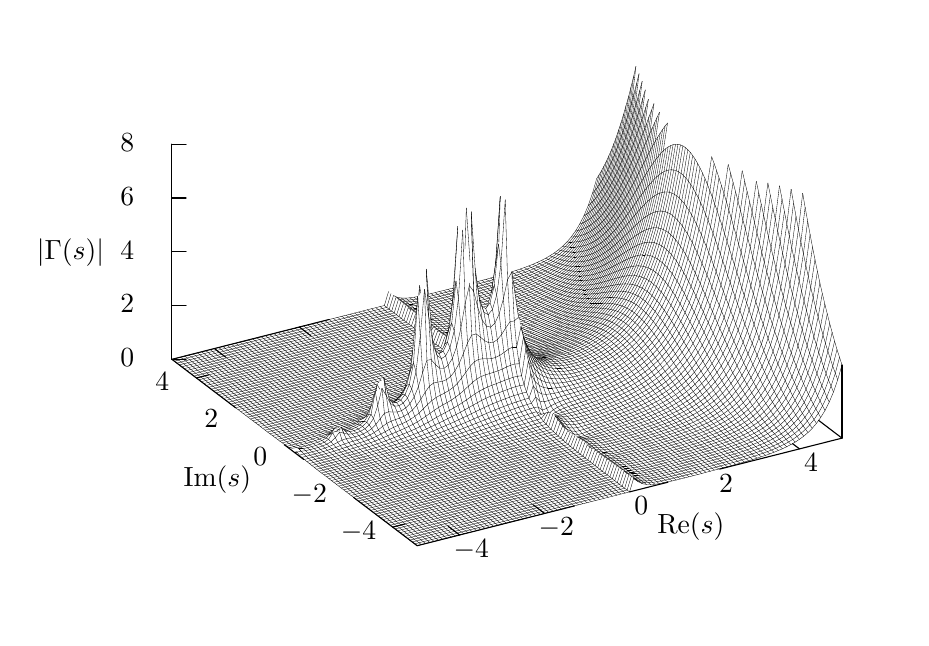
\begin{tikzpicture}[gnuplot]
%% generated with GNUPLOT 5.1p0 (Lua 5.3; terminal rev. 99, script rev. 100)
%% 水 11/21 05:26:31 2018
\path (0.000,0.000) rectangle (11.000,7.500);
\gpcolor{rgb color={0.000,0.000,0.000}}
\gpsetlinetype{gp lt border}
\gpsetdashtype{gp dt solid}
\gpsetlinewidth{0.30}
\draw[gp path] (6.492,4.572)--(6.438,4.544);
\draw[gp path] (6.469,4.528)--(6.438,4.544);
\draw[gp path] (6.384,4.519)--(6.438,4.544);
\draw[gp path] (6.546,4.603)--(6.492,4.572);
\draw[gp path] (6.523,4.558)--(6.492,4.572);
\draw[gp path] (6.415,4.502)--(6.384,4.519);
\draw[gp path] (6.330,4.495)--(6.384,4.519);
\draw[gp path] (6.577,4.590)--(6.546,4.603);
\draw[gp path] (6.600,4.638)--(6.546,4.603);
\draw[gp path] (6.276,4.474)--(6.330,4.495);
\draw[gp path] (6.362,4.477)--(6.330,4.495);
\draw[gp path] (6.222,4.454)--(6.276,4.474);
\draw[gp path] (6.308,4.455)--(6.276,4.474);
\draw[gp path] (6.654,4.678)--(6.600,4.638);
\draw[gp path] (6.631,4.628)--(6.600,4.638);
\draw[gp path] (6.254,4.434)--(6.222,4.454);
\draw[gp path] (6.169,4.435)--(6.222,4.454);
\draw[gp path] (6.685,4.670)--(6.654,4.678);
\draw[gp path] (6.708,4.725)--(6.654,4.678);
\draw[gp path] (6.200,4.415)--(6.169,4.435);
\draw[gp path] (6.115,4.417)--(6.169,4.435);
\draw[gp path] (6.501,4.513)--(6.469,4.528);
\draw[gp path] (6.523,4.558)--(6.469,4.528);
\draw[gp path] (6.415,4.502)--(6.469,4.528);
\draw[gp path] (6.362,4.477)--(6.415,4.502);
\draw[gp path] (6.447,4.485)--(6.415,4.502);
\draw[gp path] (6.555,4.544)--(6.523,4.558);
\draw[gp path] (6.577,4.590)--(6.523,4.558);
\draw[gp path] (6.308,4.455)--(6.362,4.477);
\draw[gp path] (6.393,4.460)--(6.362,4.477);
\draw[gp path] (6.146,4.396)--(6.115,4.417);
\draw[gp path] (6.061,4.400)--(6.115,4.417);
\draw[gp path] (6.608,4.579)--(6.577,4.590);
\draw[gp path] (6.631,4.628)--(6.577,4.590);
\draw[gp path] (6.254,4.434)--(6.308,4.455);
\draw[gp path] (6.339,4.437)--(6.308,4.455);
\draw[gp path] (6.739,4.719)--(6.708,4.725);
\draw[gp path] (6.762,4.778)--(6.708,4.725);
\draw[gp path] (6.285,4.415)--(6.254,4.434);
\draw[gp path] (6.092,4.378)--(6.062,4.399);
\draw[gp path] (6.200,4.415)--(6.254,4.434);
\draw[gp path] (6.662,4.618)--(6.631,4.628);
\draw[gp path] (6.685,4.670)--(6.631,4.628);
\draw[gp path] (6.146,4.396)--(6.200,4.415);
\draw[gp path] (6.231,4.395)--(6.200,4.415);
\draw[gp path] (6.478,4.469)--(6.447,4.485);
\draw[gp path] (6.393,4.460)--(6.447,4.485);
\draw[gp path] (6.501,4.513)--(6.447,4.485);
\draw[gp path] (6.092,4.378)--(6.146,4.396);
\draw[gp path] (6.177,4.376)--(6.146,4.396);
\draw[gp path] (6.555,4.544)--(6.501,4.513);
\draw[gp path] (6.532,4.499)--(6.501,4.513);
\draw[gp path] (6.739,4.719)--(6.685,4.670);
\draw[gp path] (6.716,4.663)--(6.685,4.670);
\draw[gp path] (6.424,4.443)--(6.393,4.460);
\draw[gp path] (6.339,4.437)--(6.393,4.460);
\draw[gp path] (6.586,4.531)--(6.555,4.544);
\draw[gp path] (6.608,4.579)--(6.555,4.544);
\draw[gp path] (6.285,4.415)--(6.339,4.437);
\draw[gp path] (6.370,4.419)--(6.339,4.437);
\draw[gp path] (6.793,4.776)--(6.762,4.778);
\draw[gp path] (6.816,4.841)--(6.762,4.778);
\draw[gp path] (6.066,4.370)--(6.092,4.378);
\draw[gp path] (6.123,4.357)--(6.092,4.378);
\draw[gp path] (6.640,4.568)--(6.608,4.579);
\draw[gp path] (6.662,4.618)--(6.608,4.579);
\draw[gp path] (6.316,4.396)--(6.285,4.415);
\draw[gp path] (6.231,4.395)--(6.285,4.415);
\draw[gp path] (6.262,4.375)--(6.231,4.395);
\draw[gp path] (6.177,4.376)--(6.231,4.395);
\draw[gp path] (6.770,4.715)--(6.739,4.719);
\draw[gp path] (6.793,4.776)--(6.739,4.719);
\draw[gp path] (6.694,4.609)--(6.662,4.618);
\draw[gp path] (6.716,4.663)--(6.662,4.618);
\draw[gp path] (6.208,4.355)--(6.177,4.376);
\draw[gp path] (6.123,4.357)--(6.177,4.376);
\draw[gp path] (5.792,4.320)--(5.831,4.331);
\draw[gp path] (6.424,4.443)--(6.478,4.469);
\draw[gp path] (6.509,4.454)--(6.478,4.469);
\draw[gp path] (6.532,4.499)--(6.478,4.469);
\draw[gp path] (6.455,4.426)--(6.424,4.443);
\draw[gp path] (6.370,4.419)--(6.424,4.443);
\draw[gp path] (6.563,4.485)--(6.532,4.499);
\draw[gp path] (6.586,4.531)--(6.532,4.499);
\draw[gp path] (6.401,4.401)--(6.370,4.419);
\draw[gp path] (6.316,4.396)--(6.370,4.419);
\draw[gp path] (6.070,4.340)--(6.123,4.357);
\draw[gp path] (6.154,4.337)--(6.123,4.357);
\draw[gp path] (6.640,4.568)--(6.586,4.531);
\draw[gp path] (6.617,4.519)--(6.586,4.531);
\draw[gp path] (6.262,4.375)--(6.316,4.396);
\draw[gp path] (6.347,4.378)--(6.316,4.396);
\draw[gp path] (6.770,4.715)--(6.716,4.663);
\draw[gp path] (6.748,4.657)--(6.716,4.663);
\draw[gp path] (5.823,4.298)--(5.792,4.320);
\draw[gp path] (5.738,4.305)--(5.792,4.320);
\draw[gp path] (6.847,4.843)--(6.816,4.841);
\draw[gp path] (6.870,4.916)--(6.816,4.841);
\draw[gp path] (6.100,4.319)--(6.070,4.339);
\draw[gp path] (6.293,4.356)--(6.262,4.375);
\draw[gp path] (6.208,4.355)--(6.262,4.375);
\draw[gp path] (6.671,4.558)--(6.640,4.568);
\draw[gp path] (6.694,4.609)--(6.640,4.568);
\draw[gp path] (6.847,4.843)--(6.793,4.776);
\draw[gp path] (6.824,4.776)--(6.793,4.776);
\draw[gp path] (5.769,4.283)--(5.738,4.305);
\draw[gp path] (5.684,4.291)--(5.738,4.305);
\draw[gp path] (5.823,4.298)--(5.826,4.299);
\draw[gp path] (6.239,4.336)--(6.208,4.355);
\draw[gp path] (6.154,4.337)--(6.208,4.355);
\draw[gp path] (6.725,4.602)--(6.694,4.609);
\draw[gp path] (6.748,4.657)--(6.694,4.609);
\draw[gp path] (6.185,4.316)--(6.154,4.337);
\draw[gp path] (6.100,4.319)--(6.154,4.337);
\draw[gp path] (6.486,4.411)--(6.455,4.426);
\draw[gp path] (6.401,4.401)--(6.455,4.426);
\draw[gp path] (6.509,4.454)--(6.455,4.426);
\draw[gp path] (6.540,4.440)--(6.509,4.454);
\draw[gp path] (6.563,4.485)--(6.509,4.454);
\draw[gp path] (6.432,4.384)--(6.401,4.401);
\draw[gp path] (6.347,4.378)--(6.401,4.401);
\draw[gp path] (6.801,4.712)--(6.770,4.715);
\draw[gp path] (6.824,4.776)--(6.770,4.715);
\draw[gp path] (5.769,4.283)--(5.823,4.298);
\draw[gp path] (5.825,4.296)--(5.823,4.298);
\draw[gp path] (5.715,4.268)--(5.684,4.291);
\draw[gp path] (5.630,4.276)--(5.684,4.291);
\draw[gp path] (6.594,4.472)--(6.563,4.485);
\draw[gp path] (6.617,4.519)--(6.563,4.485);
\draw[gp path] (6.293,4.356)--(6.347,4.378);
\draw[gp path] (6.378,4.360)--(6.347,4.378);
\draw[gp path] (6.075,4.311)--(6.100,4.319);
\draw[gp path] (6.131,4.298)--(6.100,4.319);
\draw[gp path] (6.648,4.508)--(6.617,4.519);
\draw[gp path] (6.671,4.558)--(6.617,4.519);
\draw[gp path] (6.239,4.336)--(6.293,4.356);
\draw[gp path] (6.324,4.337)--(6.293,4.356);
\draw[gp path] (5.800,4.260)--(5.769,4.283);
\draw[gp path] (5.715,4.268)--(5.769,4.283);
\draw[gp path] (5.620,4.273)--(5.630,4.276);
\draw[gp path] (5.661,4.253)--(5.630,4.276);
\draw[gp path] (6.185,4.316)--(6.239,4.336);
\draw[gp path] (6.270,4.316)--(6.239,4.336);
\draw[gp path] (6.779,4.653)--(6.748,4.657);
\draw[gp path] (6.801,4.712)--(6.748,4.657);
\draw[gp path] (6.725,4.602)--(6.671,4.558);
\draw[gp path] (6.702,4.549)--(6.671,4.558);
\draw[gp path] (6.216,4.296)--(6.185,4.316);
\draw[gp path] (6.131,4.298)--(6.185,4.316);
\draw[gp path] (6.901,4.923)--(6.870,4.916);
\draw[gp path] (6.924,5.005)--(6.870,4.916);
\draw[gp path] (5.661,4.253)--(5.715,4.268);
\draw[gp path] (5.746,4.245)--(5.715,4.268);
\draw[gp path] (5.800,4.260)--(5.821,4.266);
\draw[gp path] (6.878,4.847)--(6.847,4.843);
\draw[gp path] (6.901,4.923)--(6.847,4.843);
\draw[gp path] (6.517,4.396)--(6.486,4.411);
\draw[gp path] (6.432,4.384)--(6.486,4.411);
\draw[gp path] (6.540,4.440)--(6.486,4.411);
\draw[gp path] (6.378,4.360)--(6.432,4.384);
\draw[gp path] (6.463,4.368)--(6.432,4.384);
\draw[gp path] (6.571,4.426)--(6.540,4.440);
\draw[gp path] (6.594,4.472)--(6.540,4.440);
\draw[gp path] (6.324,4.337)--(6.378,4.360);
\draw[gp path] (6.409,4.343)--(6.378,4.360);
\draw[gp path] (6.079,4.281)--(6.131,4.298);
\draw[gp path] (6.162,4.277)--(6.131,4.298);
\draw[gp path] (6.878,4.847)--(6.824,4.776);
\draw[gp path] (6.855,4.777)--(6.824,4.776);
\draw[gp path] (6.625,4.460)--(6.594,4.472);
\draw[gp path] (6.648,4.508)--(6.594,4.472);
\draw[gp path] (6.779,4.653)--(6.725,4.602);
\draw[gp path] (6.756,4.596)--(6.725,4.602);
\draw[gp path] (5.818,4.247)--(5.800,4.260);
\draw[gp path] (5.746,4.245)--(5.800,4.260);
\draw[gp path] (5.692,4.230)--(5.661,4.253);
\draw[gp path] (5.624,4.243)--(5.661,4.253);
\draw[gp path] (6.270,4.316)--(6.324,4.337);
\draw[gp path] (6.355,4.319)--(6.324,4.337);
\draw[gp path] (6.108,4.259)--(6.079,4.279);
\draw[gp path] (6.216,4.296)--(6.270,4.316);
\draw[gp path] (6.301,4.297)--(6.270,4.316);
\draw[gp path] (6.833,4.712)--(6.801,4.712);
\draw[gp path] (6.679,4.499)--(6.648,4.508);
\draw[gp path] (6.702,4.549)--(6.648,4.508);
\draw[gp path] (6.855,4.777)--(6.801,4.712);
\draw[gp path] (5.777,4.222)--(5.746,4.245);
\draw[gp path] (5.692,4.230)--(5.746,4.245);
\draw[gp path] (5.638,4.216)--(5.627,4.224);
\draw[gp path] (6.248,4.277)--(6.216,4.296);
\draw[gp path] (6.162,4.277)--(6.216,4.296);
\draw[gp path] (6.756,4.596)--(6.702,4.549);
\draw[gp path] (6.733,4.542)--(6.702,4.549);
\draw[gp path] (6.194,4.257)--(6.162,4.277);
\draw[gp path] (6.810,4.650)--(6.779,4.653);
\draw[gp path] (6.833,4.712)--(6.779,4.653);
\draw[gp path] (6.108,4.259)--(6.162,4.277);
\draw[gp path] (6.517,4.396)--(6.463,4.368);
\draw[gp path] (6.409,4.343)--(6.463,4.368);
\draw[gp path] (6.494,4.352)--(6.463,4.368);
\draw[gp path] (6.571,4.426)--(6.517,4.396);
\draw[gp path] (6.548,4.381)--(6.517,4.396);
\draw[gp path] (5.638,4.216)--(5.692,4.230);
\draw[gp path] (5.723,4.207)--(5.692,4.230);
\draw[gp path] (5.777,4.222)--(5.816,4.233);
\draw[gp path] (6.355,4.319)--(6.409,4.343);
\draw[gp path] (6.441,4.326)--(6.409,4.343);
\draw[gp path] (6.625,4.460)--(6.571,4.426);
\draw[gp path] (6.602,4.414)--(6.571,4.426);
\draw[gp path] (6.301,4.297)--(6.355,4.319);
\draw[gp path] (6.387,4.301)--(6.355,4.319);
\draw[gp path] (6.083,4.251)--(6.108,4.259);
\draw[gp path] (6.140,4.239)--(6.108,4.259);
\draw[gp path] (6.656,4.450)--(6.625,4.460);
\draw[gp path] (6.679,4.499)--(6.625,4.460);
\draw[gp path] (6.248,4.277)--(6.301,4.297);
\draw[gp path] (6.333,4.279)--(6.301,4.297);
\draw[gp path] (5.809,4.200)--(5.777,4.222);
\draw[gp path] (5.723,4.207)--(5.777,4.222);
\draw[gp path] (5.629,4.213)--(5.638,4.216);
\draw[gp path] (5.669,4.193)--(5.638,4.216);
\draw[gp path] (6.909,4.853)--(6.878,4.847);
\draw[gp path] (6.932,4.931)--(6.878,4.847);
\draw[gp path] (6.810,4.650)--(6.756,4.596);
\draw[gp path] (6.787,4.591)--(6.756,4.596);
\draw[gp path] (6.955,5.017)--(6.901,4.923);
\draw[gp path] (6.932,4.931)--(6.901,4.923);
\draw[gp path] (5.306,4.191)--(5.320,4.195);
\draw[gp path] (6.194,4.257)--(6.248,4.277);
\draw[gp path] (6.279,4.257)--(6.248,4.277);
\draw[gp path] (6.887,4.780)--(6.855,4.777);
\draw[gp path] (6.909,4.853)--(6.855,4.777);
\draw[gp path] (6.710,4.490)--(6.679,4.499);
\draw[gp path] (6.733,4.542)--(6.679,4.499);
\draw[gp path] (6.955,5.017)--(6.924,5.005);
\draw[gp path] (6.978,5.111)--(6.924,5.005);
\draw[gp path] (5.755,4.185)--(5.723,4.207);
\draw[gp path] (5.669,4.193)--(5.723,4.207);
\draw[gp path] (5.809,4.200)--(5.812,4.201);
\draw[gp path] (6.140,4.239)--(6.194,4.257);
\draw[gp path] (6.225,4.237)--(6.194,4.257);
\draw[gp path] (6.864,4.712)--(6.833,4.712);
\draw[gp path] (6.887,4.780)--(6.833,4.712);
\draw[gp path] (5.319,4.181)--(5.306,4.191);
\draw[gp path] (5.252,4.177)--(5.306,4.191);
\draw[gp path] (6.548,4.381)--(6.494,4.352);
\draw[gp path] (6.441,4.326)--(6.494,4.352);
\draw[gp path] (6.526,4.337)--(6.494,4.352);
\draw[gp path] (6.387,4.301)--(6.441,4.326);
\draw[gp path] (6.472,4.310)--(6.441,4.326);
\draw[gp path] (6.602,4.414)--(6.548,4.381);
\draw[gp path] (6.580,4.368)--(6.548,4.381);
\draw[gp path] (6.171,4.218)--(6.140,4.239);
\draw[gp path] (6.088,4.222)--(6.140,4.239);
\draw[gp path] (6.418,4.284)--(6.387,4.301);
\draw[gp path] (6.333,4.279)--(6.387,4.301);
\draw[gp path] (6.787,4.591)--(6.733,4.542);
\draw[gp path] (6.764,4.536)--(6.733,4.542);
\draw[gp path] (5.811,4.198)--(5.809,4.200);
\draw[gp path] (5.755,4.185)--(5.809,4.200);
\draw[gp path] (5.633,4.183)--(5.669,4.193);
\draw[gp path] (5.701,4.170)--(5.669,4.193);
\draw[gp path] (6.634,4.402)--(6.602,4.414);
\draw[gp path] (6.656,4.450)--(6.602,4.414);
\draw[gp path] (6.364,4.261)--(6.333,4.279);
\draw[gp path] (6.279,4.257)--(6.333,4.279);
\draw[gp path] (6.864,4.712)--(6.810,4.650);
\draw[gp path] (6.841,4.649)--(6.810,4.650);
\draw[gp path] (5.198,4.163)--(5.252,4.177);
\draw[gp path] (5.283,4.154)--(5.252,4.177);
\draw[gp path] (6.117,4.200)--(6.088,4.219);
\draw[gp path] (6.310,4.239)--(6.279,4.257);
\draw[gp path] (6.225,4.237)--(6.279,4.257);
\draw[gp path] (6.710,4.490)--(6.656,4.450);
\draw[gp path] (6.687,4.440)--(6.656,4.450);
\draw[gp path] (5.701,4.170)--(5.755,4.185);
\draw[gp path] (5.786,4.162)--(5.755,4.185);
\draw[gp path] (5.647,4.155)--(5.635,4.163);
\draw[gp path] (6.256,4.218)--(6.225,4.237);
\draw[gp path] (6.171,4.218)--(6.225,4.237);
\draw[gp path] (5.283,4.154)--(5.318,4.163);
\draw[gp path] (5.229,4.141)--(5.198,4.163);
\draw[gp path] (5.144,4.150)--(5.198,4.163);
\draw[gp path] (6.818,4.588)--(6.787,4.591);
\draw[gp path] (6.841,4.649)--(6.787,4.591);
\draw[gp path] (6.741,4.482)--(6.710,4.490);
\draw[gp path] (6.764,4.536)--(6.710,4.490);
\draw[gp path] (6.202,4.198)--(6.171,4.218);
\draw[gp path] (6.117,4.200)--(6.171,4.218);
\draw[gp path] (5.647,4.155)--(5.701,4.170);
\draw[gp path] (5.732,4.148)--(5.701,4.170);
\draw[gp path] (5.786,4.162)--(5.807,4.168);
\draw[gp path] (6.503,4.294)--(6.472,4.310);
\draw[gp path] (6.526,4.337)--(6.472,4.310);
\draw[gp path] (6.418,4.284)--(6.472,4.310);
\draw[gp path] (6.580,4.368)--(6.526,4.337);
\draw[gp path] (6.557,4.323)--(6.526,4.337);
\draw[gp path] (6.364,4.261)--(6.418,4.284);
\draw[gp path] (6.449,4.268)--(6.418,4.284);
\draw[gp path] (6.611,4.355)--(6.580,4.368);
\draw[gp path] (6.634,4.402)--(6.580,4.368);
\draw[gp path] (5.229,4.141)--(5.283,4.154);
\draw[gp path] (5.315,4.131)--(5.283,4.154);
\draw[gp path] (6.310,4.239)--(6.364,4.261);
\draw[gp path] (6.395,4.243)--(6.364,4.261);
\draw[gp path] (6.963,4.943)--(6.909,4.853);
\draw[gp path] (6.941,4.861)--(6.909,4.853);
\draw[gp path] (5.090,4.136)--(5.144,4.150);
\draw[gp path] (6.092,4.192)--(6.117,4.200);
\draw[gp path] (6.148,4.180)--(6.117,4.200);
\draw[gp path] (5.176,4.127)--(5.144,4.150);
\draw[gp path] (6.918,4.785)--(6.887,4.780);
\draw[gp path] (6.941,4.861)--(6.887,4.780);
\draw[gp path] (6.986,5.032)--(6.932,4.931);
\draw[gp path] (6.963,4.943)--(6.932,4.931);
\draw[gp path] (6.687,4.440)--(6.634,4.402);
\draw[gp path] (6.665,4.391)--(6.634,4.402);
\draw[gp path] (6.256,4.218)--(6.310,4.239);
\draw[gp path] (6.341,4.220)--(6.310,4.239);
\draw[gp path] (5.732,4.148)--(5.786,4.162);
\draw[gp path] (5.804,4.150)--(5.786,4.162);
\draw[gp path] (5.678,4.133)--(5.647,4.155);
\draw[gp path] (5.637,4.154)--(5.647,4.155);
\draw[gp path] (6.918,4.785)--(6.864,4.712);
\draw[gp path] (6.895,4.715)--(6.864,4.712);
\draw[gp path] (6.795,4.531)--(6.764,4.536);
\draw[gp path] (6.818,4.588)--(6.764,4.536);
\draw[gp path] (5.315,4.131)--(5.316,4.132);
\draw[gp path] (6.287,4.199)--(6.256,4.218);
\draw[gp path] (6.202,4.198)--(6.256,4.218);
\draw[gp path] (5.176,4.127)--(5.229,4.141);
\draw[gp path] (5.261,4.117)--(5.229,4.141);
\draw[gp path] (6.986,5.032)--(6.955,5.017);
\draw[gp path] (7.009,5.130)--(6.955,5.017);
\draw[gp path] (5.036,4.123)--(5.090,4.136);
\draw[gp path] (6.719,4.431)--(6.687,4.440);
\draw[gp path] (5.122,4.113)--(5.090,4.136);
\draw[gp path] (6.741,4.482)--(6.687,4.440);
\draw[gp path] (5.763,4.126)--(5.732,4.148);
\draw[gp path] (5.678,4.133)--(5.732,4.148);
\draw[gp path] (6.148,4.180)--(6.202,4.198);
\draw[gp path] (6.233,4.179)--(6.202,4.198);
\draw[gp path] (6.895,4.715)--(6.841,4.649);
\draw[gp path] (6.872,4.649)--(6.841,4.649);
\draw[gp path] (5.261,4.117)--(5.315,4.131);
\draw[gp path] (5.316,4.130)--(5.315,4.131);
\draw[gp path] (5.207,4.104)--(5.176,4.127);
\draw[gp path] (5.122,4.113)--(5.176,4.127);
\draw[gp path] (6.534,4.280)--(6.503,4.294);
\draw[gp path] (6.449,4.268)--(6.503,4.294);
\draw[gp path] (6.557,4.323)--(6.503,4.294);
\draw[gp path] (6.480,4.252)--(6.449,4.268);
\draw[gp path] (6.395,4.243)--(6.449,4.268);
\draw[gp path] (6.588,4.310)--(6.557,4.323);
\draw[gp path] (6.611,4.355)--(6.557,4.323);
\draw[gp path] (6.096,4.162)--(6.148,4.180);
\draw[gp path] (6.179,4.159)--(6.148,4.180);
\draw[gp path] (5.068,4.100)--(5.036,4.123);
\draw[gp path] (5.004,4.115)--(5.036,4.123);
\draw[gp path] (6.426,4.226)--(6.395,4.243);
\draw[gp path] (6.341,4.220)--(6.395,4.243);
\draw[gp path] (5.641,4.123)--(5.678,4.133);
\draw[gp path] (5.709,4.111)--(5.678,4.133);
\draw[gp path] (6.773,4.476)--(6.741,4.482);
\draw[gp path] (6.795,4.531)--(6.741,4.482);
\draw[gp path] (5.763,4.126)--(5.802,4.137);
\draw[gp path] (6.665,4.391)--(6.611,4.355);
\draw[gp path] (6.642,4.344)--(6.611,4.355);
\draw[gp path] (6.287,4.199)--(6.341,4.220);
\draw[gp path] (6.872,4.649)--(6.818,4.588);
\draw[gp path] (6.849,4.587)--(6.818,4.588);
\draw[gp path] (6.372,4.202)--(6.341,4.220);
\draw[gp path] (7.009,5.130)--(6.978,5.111);
\draw[gp path] (7.032,5.240)--(6.978,5.111);
\draw[gp path] (5.292,4.094)--(5.261,4.117);
\draw[gp path] (5.207,4.104)--(5.261,4.117);
\draw[gp path] (6.125,4.142)--(6.097,4.160);
\draw[gp path] (5.068,4.100)--(5.122,4.113);
\draw[gp path] (5.153,4.090)--(5.122,4.113);
\draw[gp path] (6.318,4.180)--(6.287,4.199);
\draw[gp path] (6.233,4.179)--(6.287,4.199);
\draw[gp path] (6.719,4.431)--(6.665,4.391);
\draw[gp path] (6.696,4.381)--(6.665,4.391);
\draw[gp path] (5.793,4.104)--(5.763,4.126);
\draw[gp path] (5.709,4.111)--(5.763,4.126);
\draw[gp path] (5.655,4.096)--(5.644,4.104);
\draw[gp path] (5.014,4.087)--(5.006,4.093);
\draw[gp path] (5.292,4.094)--(5.314,4.100);
\draw[gp path] (6.264,4.159)--(6.233,4.179);
\draw[gp path] (6.179,4.159)--(6.233,4.179);
\draw[gp path] (5.238,4.080)--(5.207,4.104);
\draw[gp path] (5.153,4.090)--(5.207,4.104);
\draw[gp path] (6.827,4.528)--(6.795,4.531);
\draw[gp path] (6.849,4.587)--(6.795,4.531);
\draw[gp path] (5.014,4.087)--(5.068,4.100);
\draw[gp path] (5.099,4.077)--(5.068,4.100);
\draw[gp path] (6.773,4.476)--(6.719,4.431);
\draw[gp path] (6.750,4.423)--(6.719,4.431);
\draw[gp path] (6.972,4.871)--(6.918,4.785);
\draw[gp path] (6.949,4.792)--(6.918,4.785);
\draw[gp path] (5.740,4.088)--(5.709,4.111);
\draw[gp path] (5.655,4.096)--(5.709,4.111);
\draw[gp path] (6.210,4.141)--(6.179,4.159);
\draw[gp path] (6.972,4.871)--(6.941,4.861);
\draw[gp path] (6.995,4.956)--(6.941,4.861);
\draw[gp path] (6.125,4.142)--(6.179,4.159);
\draw[gp path] (6.511,4.236)--(6.480,4.252);
\draw[gp path] (6.534,4.280)--(6.480,4.252);
\draw[gp path] (6.426,4.226)--(6.480,4.252);
\draw[gp path] (6.949,4.792)--(6.895,4.715);
\draw[gp path] (6.926,4.719)--(6.895,4.715);
\draw[gp path] (6.588,4.310)--(6.534,4.280);
\draw[gp path] (6.565,4.266)--(6.534,4.280);
\draw[gp path] (6.372,4.202)--(6.426,4.226);
\draw[gp path] (6.457,4.210)--(6.426,4.226);
\draw[gp path] (5.238,4.080)--(5.292,4.094);
\draw[gp path] (5.312,4.079)--(5.292,4.094);
\draw[gp path] (6.642,4.344)--(6.588,4.310);
\draw[gp path] (6.619,4.298)--(6.588,4.310);
\draw[gp path] (6.995,4.956)--(6.963,4.943);
\draw[gp path] (7.017,5.050)--(6.963,4.943);
\draw[gp path] (5.099,4.077)--(5.153,4.090);
\draw[gp path] (5.184,4.067)--(5.153,4.090);
\draw[gp path] (6.403,4.185)--(6.372,4.202);
\draw[gp path] (6.318,4.180)--(6.372,4.202);
\draw[gp path] (6.101,4.134)--(6.125,4.142);
\draw[gp path] (6.156,4.122)--(6.125,4.142);
\draw[gp path] (5.740,4.088)--(5.792,4.103);
\draw[gp path] (5.645,4.093)--(5.655,4.096);
\draw[gp path] (6.903,4.651)--(6.872,4.649);
\draw[gp path] (6.926,4.719)--(6.872,4.649);
\draw[gp path] (5.686,4.073)--(5.655,4.096);
\draw[gp path] (5.006,4.085)--(5.014,4.087);
\draw[gp path] (5.045,4.064)--(5.014,4.087);
\draw[gp path] (6.696,4.381)--(6.642,4.344);
\draw[gp path] (6.673,4.333)--(6.642,4.344);
\draw[gp path] (6.264,4.159)--(6.318,4.180);
\draw[gp path] (6.349,4.162)--(6.318,4.180);
\draw[gp path] (6.827,4.528)--(6.773,4.476);
\draw[gp path] (6.804,4.471)--(6.773,4.476);
\draw[gp path] (5.269,4.057)--(5.238,4.080);
\draw[gp path] (5.184,4.067)--(5.238,4.080);
\draw[gp path] (4.821,4.077)--(4.867,4.085);
\draw[gp path] (6.295,4.141)--(6.264,4.159);
\draw[gp path] (6.210,4.141)--(6.264,4.159);
\draw[gp path] (7.017,5.050)--(6.986,5.032);
\draw[gp path] (7.040,5.152)--(6.986,5.032);
\draw[gp path] (5.130,4.053)--(5.099,4.077);
\draw[gp path] (5.045,4.064)--(5.099,4.077);
\draw[gp path] (6.750,4.423)--(6.696,4.381);
\draw[gp path] (6.727,4.373)--(6.696,4.381);
\draw[gp path] (5.686,4.073)--(5.740,4.088);
\draw[gp path] (5.771,4.066)--(5.740,4.088);
\draw[gp path] (6.880,4.587)--(6.849,4.587);
\draw[gp path] (6.903,4.651)--(6.849,4.587);
\draw[gp path] (6.156,4.122)--(6.210,4.141);
\draw[gp path] (6.241,4.121)--(6.210,4.141);
\draw[gp path] (5.269,4.057)--(5.311,4.068);
\draw[gp path] (5.130,4.053)--(5.184,4.067);
\draw[gp path] (5.215,4.043)--(5.184,4.067);
\draw[gp path] (6.457,4.210)--(6.511,4.236);
\draw[gp path] (6.565,4.266)--(6.511,4.236);
\draw[gp path] (6.542,4.222)--(6.511,4.236);
\draw[gp path] (6.403,4.185)--(6.457,4.210);
\draw[gp path] (6.488,4.194)--(6.457,4.210);
\draw[gp path] (6.187,4.102)--(6.156,4.122);
\draw[gp path] (6.105,4.104)--(6.156,4.122);
\draw[gp path] (5.009,4.056)--(5.045,4.064);
\draw[gp path] (5.076,4.040)--(5.045,4.064);
\draw[gp path] (5.717,4.050)--(5.686,4.073);
\draw[gp path] (5.651,4.064)--(5.686,4.073);
\draw[gp path] (6.596,4.252)--(6.565,4.266);
\draw[gp path] (6.619,4.298)--(6.565,4.266);
\draw[gp path] (4.767,4.069)--(4.821,4.077);
\draw[gp path] (4.852,4.053)--(4.821,4.077);
\draw[gp path] (5.771,4.066)--(5.782,4.069);
\draw[gp path] (6.804,4.471)--(6.750,4.423);
\draw[gp path] (6.781,4.417)--(6.750,4.423);
\draw[gp path] (6.434,4.168)--(6.403,4.185);
\draw[gp path] (6.349,4.162)--(6.403,4.185);
\draw[gp path] (6.858,4.526)--(6.827,4.528);
\draw[gp path] (6.880,4.587)--(6.827,4.528);
\draw[gp path] (6.673,4.333)--(6.619,4.298);
\draw[gp path] (6.650,4.286)--(6.619,4.298);
\draw[gp path] (5.215,4.043)--(5.269,4.057);
\draw[gp path] (5.300,4.034)--(5.269,4.057);
\draw[gp path] (6.380,4.145)--(6.349,4.162);
\draw[gp path] (6.295,4.141)--(6.349,4.162);
\draw[gp path] (4.852,4.053)--(4.865,4.056);
\draw[gp path] (6.133,4.083)--(6.106,4.101);
\draw[gp path] (7.040,5.152)--(7.009,5.130);
\draw[gp path] (7.063,5.267)--(7.009,5.130);
\draw[gp path] (5.161,4.030)--(5.130,4.053);
\draw[gp path] (5.076,4.040)--(5.130,4.053);
\draw[gp path] (6.241,4.121)--(6.295,4.141);
\draw[gp path] (6.326,4.123)--(6.295,4.141);
\draw[gp path] (5.717,4.050)--(5.771,4.066);
\draw[gp path] (5.780,4.059)--(5.771,4.066);
\draw[gp path] (5.663,4.036)--(5.659,4.039);
\draw[gp path] (6.727,4.373)--(6.673,4.333);
\draw[gp path] (6.704,4.323)--(6.673,4.333);
\draw[gp path] (5.022,4.028)--(5.011,4.036);
\draw[gp path] (5.300,4.034)--(5.309,4.036);
\draw[gp path] (7.003,4.884)--(6.949,4.792);
\draw[gp path] (6.980,4.802)--(6.949,4.792);
\draw[gp path] (6.957,4.726)--(6.926,4.719);
\draw[gp path] (6.980,4.802)--(6.926,4.719);
\draw[gp path] (6.273,4.102)--(6.241,4.121);
\draw[gp path] (6.187,4.102)--(6.241,4.121);
\draw[gp path] (5.246,4.020)--(5.215,4.043);
\draw[gp path] (5.161,4.030)--(5.215,4.043);
\draw[gp path] (4.798,4.045)--(4.767,4.069);
\draw[gp path] (4.713,4.065)--(4.767,4.069);
\draw[gp path] (7.026,4.973)--(6.972,4.871);
\draw[gp path] (7.003,4.884)--(6.972,4.871);
\draw[gp path] (6.858,4.526)--(6.804,4.471);
\draw[gp path] (6.835,4.468)--(6.804,4.471);
\draw[gp path] (5.107,4.017)--(5.076,4.040);
\draw[gp path] (5.022,4.028)--(5.076,4.040);
\draw[gp path] (4.864,4.044)--(4.852,4.053);
\draw[gp path] (4.798,4.045)--(4.852,4.053);
\draw[gp path] (5.748,4.028)--(5.717,4.050);
\draw[gp path] (5.663,4.036)--(5.717,4.050);
\draw[gp path] (6.957,4.726)--(6.903,4.651);
\draw[gp path] (6.934,4.655)--(6.903,4.651);
\draw[gp path] (6.758,4.365)--(6.727,4.373);
\draw[gp path] (6.781,4.417)--(6.727,4.373);
\draw[gp path] (6.219,4.082)--(6.187,4.102);
\draw[gp path] (6.133,4.083)--(6.187,4.102);
\draw[gp path] (5.308,4.027)--(5.300,4.034);
\draw[gp path] (5.246,4.020)--(5.300,4.034);
\draw[gp path] (6.542,4.222)--(6.488,4.194);
\draw[gp path] (6.434,4.168)--(6.488,4.194);
\draw[gp path] (6.520,4.179)--(6.488,4.194);
\draw[gp path] (6.573,4.208)--(6.542,4.222);
\draw[gp path] (6.596,4.252)--(6.542,4.222);
\draw[gp path] (7.048,5.070)--(6.995,4.956);
\draw[gp path] (7.026,4.973)--(6.995,4.956);
\draw[gp path] (6.466,4.153)--(6.434,4.168);
\draw[gp path] (6.380,4.145)--(6.434,4.168);
\draw[gp path] (5.192,4.006)--(5.161,4.030);
\draw[gp path] (5.107,4.017)--(5.161,4.030);
\draw[gp path] (6.627,4.240)--(6.596,4.252);
\draw[gp path] (6.650,4.286)--(6.596,4.252);
\draw[gp path] (6.912,4.588)--(6.880,4.587);
\draw[gp path] (6.934,4.655)--(6.880,4.587);
\draw[gp path] (6.109,4.075)--(6.133,4.083);
\draw[gp path] (6.165,4.063)--(6.133,4.083);
\draw[gp path] (6.412,4.128)--(6.380,4.145);
\draw[gp path] (6.326,4.123)--(6.380,4.145);
\draw[gp path] (5.660,4.035)--(5.663,4.036);
\draw[gp path] (5.695,4.013)--(5.663,4.036);
\draw[gp path] (5.748,4.028)--(5.773,4.035);
\draw[gp path] (5.053,4.004)--(5.022,4.028);
\draw[gp path] (5.012,4.026)--(5.022,4.028);
\draw[gp path] (6.704,4.323)--(6.650,4.286);
\draw[gp path] (6.681,4.275)--(6.650,4.286);
\draw[gp path] (6.273,4.102)--(6.326,4.123);
\draw[gp path] (6.358,4.105)--(6.326,4.123);
\draw[gp path] (6.835,4.468)--(6.781,4.417);
\draw[gp path] (6.812,4.412)--(6.781,4.417);
\draw[gp path] (4.744,4.041)--(4.713,4.065);
\draw[gp path] (4.659,4.066)--(4.713,4.065);
\draw[gp path] (7.086,5.395)--(7.032,5.240);
\draw[gp path] (7.063,5.267)--(7.032,5.240);
\draw[gp path] (5.192,4.006)--(5.246,4.020);
\draw[gp path] (5.277,3.996)--(5.246,4.020);
\draw[gp path] (4.829,4.022)--(4.798,4.045);
\draw[gp path] (4.744,4.041)--(4.798,4.045);
\draw[gp path] (6.304,4.084)--(6.273,4.102);
\draw[gp path] (6.219,4.082)--(6.273,4.102);
\draw[gp path] (5.138,3.993)--(5.107,4.017);
\draw[gp path] (5.053,4.004)--(5.107,4.017);
\draw[gp path] (4.829,4.022)--(4.862,4.026);
\draw[gp path] (6.889,4.525)--(6.858,4.526);
\draw[gp path] (6.912,4.588)--(6.858,4.526);
\draw[gp path] (5.695,4.013)--(5.748,4.028);
\draw[gp path] (5.767,4.015)--(5.748,4.028);
\draw[gp path] (7.048,5.070)--(7.017,5.050);
\draw[gp path] (7.071,5.178)--(7.017,5.050);
\draw[gp path] (6.758,4.365)--(6.704,4.323);
\draw[gp path] (6.735,4.315)--(6.704,4.323);
\draw[gp path] (5.277,3.996)--(5.306,4.003);
\draw[gp path] (6.165,4.063)--(6.219,4.082);
\draw[gp path] (6.250,4.063)--(6.219,4.082);
\draw[gp path] (5.138,3.993)--(5.192,4.006);
\draw[gp path] (5.223,3.982)--(5.192,4.006);
\draw[gp path] (5.726,3.990)--(5.695,4.013);
\draw[gp path] (5.669,4.006)--(5.695,4.013);
\draw[gp path] (5.084,3.980)--(5.053,4.004);
\draw[gp path] (5.014,3.996)--(5.053,4.004);
\draw[gp path] (6.114,4.046)--(6.165,4.063);
\draw[gp path] (6.196,4.043)--(6.165,4.063);
\draw[gp path] (6.466,4.153)--(6.520,4.179);
\draw[gp path] (6.551,4.165)--(6.520,4.179);
\draw[gp path] (6.573,4.208)--(6.520,4.179);
\draw[gp path] (6.497,4.138)--(6.466,4.153);
\draw[gp path] (6.412,4.128)--(6.466,4.153);
\draw[gp path] (6.605,4.195)--(6.573,4.208);
\draw[gp path] (6.627,4.240)--(6.573,4.208);
\draw[gp path] (6.789,4.359)--(6.758,4.365);
\draw[gp path] (6.812,4.412)--(6.758,4.365);
\draw[gp path] (6.889,4.525)--(6.835,4.468);
\draw[gp path] (6.866,4.465)--(6.835,4.468);
\draw[gp path] (6.443,4.112)--(6.412,4.128);
\draw[gp path] (6.358,4.105)--(6.412,4.128);
\draw[gp path] (4.775,4.017)--(4.744,4.041);
\draw[gp path] (4.690,4.042)--(4.744,4.041);
\draw[gp path] (5.302,3.977)--(5.277,3.996);
\draw[gp path] (5.223,3.982)--(5.277,3.996);
\draw[gp path] (4.775,4.017)--(4.829,4.022);
\draw[gp path] (4.859,3.998)--(4.829,4.022);
\draw[gp path] (6.659,4.229)--(6.627,4.240);
\draw[gp path] (6.681,4.275)--(6.627,4.240);
\draw[gp path] (6.304,4.084)--(6.358,4.105);
\draw[gp path] (6.389,4.088)--(6.358,4.105);
\draw[gp path] (5.169,3.969)--(5.138,3.993);
\draw[gp path] (5.084,3.980)--(5.138,3.993);
\draw[gp path] (6.142,4.025)--(6.114,4.042);
\draw[gp path] (4.690,4.042)--(4.659,4.066);
\draw[gp path] (4.605,4.077)--(4.659,4.066);
\draw[gp path] (6.988,4.734)--(6.957,4.726);
\draw[gp path] (7.011,4.813)--(6.957,4.726);
\draw[gp path] (7.011,4.813)--(6.980,4.802);
\draw[gp path] (7.034,4.899)--(6.980,4.802);
\draw[gp path] (5.726,3.990)--(5.763,4.001);
\draw[gp path] (6.250,4.063)--(6.304,4.084);
\draw[gp path] (6.335,4.065)--(6.304,4.084);
\draw[gp path] (6.988,4.734)--(6.934,4.655);
\draw[gp path] (6.966,4.661)--(6.934,4.655);
\draw[gp path] (6.735,4.315)--(6.681,4.275);
\draw[gp path] (6.713,4.266)--(6.681,4.275);
\draw[gp path] (5.030,3.968)--(5.016,3.979);
\draw[gp path] (7.094,5.297)--(7.040,5.152);
\draw[gp path] (7.071,5.178)--(7.040,5.152);
\draw[gp path] (5.255,3.958)--(5.223,3.982);
\draw[gp path] (5.169,3.969)--(5.223,3.982);
\draw[gp path] (7.057,4.992)--(7.003,4.884);
\draw[gp path] (7.034,4.899)--(7.003,4.884);
\draw[gp path] (6.196,4.043)--(6.250,4.063);
\draw[gp path] (6.281,4.044)--(6.250,4.063);
\draw[gp path] (6.943,4.592)--(6.912,4.588);
\draw[gp path] (6.966,4.661)--(6.912,4.588);
\draw[gp path] (6.866,4.465)--(6.812,4.412);
\draw[gp path] (6.843,4.408)--(6.812,4.412);
\draw[gp path] (5.030,3.968)--(5.084,3.980);
\draw[gp path] (5.115,3.956)--(5.084,3.980);
\draw[gp path] (4.474,3.948)--(4.443,3.971);
\draw[gp path] (4.497,4.150)--(4.443,3.971);
\draw[gp path] (4.389,3.958)--(4.443,3.971);
\draw[gp path] (5.679,3.977)--(5.726,3.990);
\draw[gp path] (5.754,3.970)--(5.726,3.990);
\draw[gp path] (6.766,4.307)--(6.735,4.315);
\draw[gp path] (6.789,4.359)--(6.735,4.315);
\draw[gp path] (4.721,4.018)--(4.775,4.017);
\draw[gp path] (4.806,3.993)--(4.775,4.017);
\draw[gp path] (6.142,4.025)--(6.196,4.043);
\draw[gp path] (6.227,4.024)--(6.196,4.043);
\draw[gp path] (4.806,3.993)--(4.859,3.998);
\draw[gp path] (5.255,3.958)--(5.301,3.970);
\draw[gp path] (5.115,3.956)--(5.169,3.969);
\draw[gp path] (5.201,3.944)--(5.169,3.969);
\draw[gp path] (4.636,4.052)--(4.690,4.042);
\draw[gp path] (4.721,4.018)--(4.690,4.042);
\draw[gp path] (7.080,5.094)--(7.026,4.973);
\draw[gp path] (7.057,4.992)--(7.026,4.973);
\draw[gp path] (6.528,4.123)--(6.497,4.138);
\draw[gp path] (6.551,4.165)--(6.497,4.138);
\draw[gp path] (6.443,4.112)--(6.497,4.138);
\draw[gp path] (6.943,4.592)--(6.889,4.525);
\draw[gp path] (6.920,4.526)--(6.889,4.525);
\draw[gp path] (6.605,4.195)--(6.551,4.165);
\draw[gp path] (6.582,4.152)--(6.551,4.165);
\draw[gp path] (6.474,4.096)--(6.443,4.112);
\draw[gp path] (6.389,4.088)--(6.443,4.112);
\draw[gp path] (6.118,4.017)--(6.142,4.025);
\draw[gp path] (6.173,4.005)--(6.142,4.025);
\draw[gp path] (6.636,4.183)--(6.605,4.195);
\draw[gp path] (6.659,4.229)--(6.605,4.195);
\draw[gp path] (4.335,3.944)--(4.389,3.958);
\draw[gp path] (4.420,3.934)--(4.389,3.958);
\draw[gp path] (6.335,4.065)--(6.389,4.088);
\draw[gp path] (6.420,4.071)--(6.389,4.088);
\draw[gp path] (5.062,3.944)--(5.030,3.968);
\draw[gp path] (5.017,3.966)--(5.030,3.968);
\draw[gp path] (5.286,3.934)--(5.255,3.958);
\draw[gp path] (5.201,3.944)--(5.255,3.958);
\draw[gp path] (6.366,4.048)--(6.335,4.065);
\draw[gp path] (6.281,4.044)--(6.335,4.065);
\draw[gp path] (6.690,4.218)--(6.659,4.229);
\draw[gp path] (6.713,4.266)--(6.659,4.229);
\draw[gp path] (6.843,4.408)--(6.789,4.359);
\draw[gp path] (6.820,4.353)--(6.789,4.359);
\draw[gp path] (5.062,3.944)--(5.115,3.956);
\draw[gp path] (5.147,3.931)--(5.115,3.956);
\draw[gp path] (4.559,4.098)--(4.605,4.077);
\draw[gp path] (4.636,4.052)--(4.605,4.077);
\draw[gp path] (4.528,4.124)--(4.474,3.948);
\draw[gp path] (4.420,3.934)--(4.474,3.948);
\draw[gp path] (4.505,3.924)--(4.474,3.948);
\draw[gp path] (6.920,4.526)--(6.866,4.465);
\draw[gp path] (6.897,4.465)--(6.866,4.465);
\draw[gp path] (6.312,4.026)--(6.281,4.044);
\draw[gp path] (6.227,4.024)--(6.281,4.044);
\draw[gp path] (5.703,3.953)--(5.751,3.966);
\draw[gp path] (4.752,3.993)--(4.806,3.993);
\draw[gp path] (4.837,3.968)--(4.806,3.993);
\draw[gp path] (4.837,3.968)--(4.857,3.970);
\draw[gp path] (4.281,3.931)--(4.335,3.944);
\draw[gp path] (4.366,3.920)--(4.335,3.944);
\draw[gp path] (5.286,3.934)--(5.296,3.937);
\draw[gp path] (6.744,4.257)--(6.713,4.266);
\draw[gp path] (6.766,4.307)--(6.713,4.266);
\draw[gp path] (5.232,3.919)--(5.201,3.944);
\draw[gp path] (5.147,3.931)--(5.201,3.944);
\draw[gp path] (7.117,5.432)--(7.063,5.267);
\draw[gp path] (7.094,5.297)--(7.063,5.267);
\draw[gp path] (7.080,5.094)--(7.048,5.070);
\draw[gp path] (7.102,5.206)--(7.048,5.070);
\draw[gp path] (4.752,3.993)--(4.721,4.018);
\draw[gp path] (4.667,4.027)--(4.721,4.018);
\draw[gp path] (6.258,4.005)--(6.227,4.024);
\draw[gp path] (6.173,4.005)--(6.227,4.024);
\draw[gp path] (4.366,3.920)--(4.420,3.934);
\draw[gp path] (4.451,3.910)--(4.420,3.934);
\draw[gp path] (5.093,3.919)--(5.062,3.944);
\draw[gp path] (5.020,3.935)--(5.062,3.944);
\draw[gp path] (6.122,3.987)--(6.173,4.005);
\draw[gp path] (6.204,3.985)--(6.173,4.005);
\draw[gp path] (5.295,3.927)--(5.286,3.934);
\draw[gp path] (5.232,3.919)--(5.286,3.934);
\draw[gp path] (4.227,3.917)--(4.281,3.931);
\draw[gp path] (4.312,3.907)--(4.281,3.931);
\draw[gp path] (6.582,4.152)--(6.528,4.123);
\draw[gp path] (6.559,4.109)--(6.528,4.123);
\draw[gp path] (6.474,4.096)--(6.528,4.123);
\draw[gp path] (7.042,4.827)--(6.988,4.734);
\draw[gp path] (6.897,4.465)--(6.843,4.408);
\draw[gp path] (7.020,4.745)--(6.988,4.734);
\draw[gp path] (6.874,4.406)--(6.843,4.408);
\draw[gp path] (6.420,4.071)--(6.474,4.096);
\draw[gp path] (6.505,4.081)--(6.474,4.096);
\draw[gp path] (6.798,4.301)--(6.766,4.307);
\draw[gp path] (6.820,4.353)--(6.766,4.307);
\draw[gp path] (6.997,4.668)--(6.966,4.661);
\draw[gp path] (7.020,4.745)--(6.966,4.661);
\draw[gp path] (6.636,4.183)--(6.582,4.152);
\draw[gp path] (6.613,4.140)--(6.582,4.152);
\draw[gp path] (6.366,4.048)--(6.420,4.071);
\draw[gp path] (6.451,4.055)--(6.420,4.071);
\draw[gp path] (5.093,3.919)--(5.147,3.931);
\draw[gp path] (5.178,3.906)--(5.147,3.931);
\draw[gp path] (4.667,4.027)--(4.636,4.052);
\draw[gp path] (4.591,4.073)--(4.636,4.052);
\draw[gp path] (7.065,4.916)--(7.011,4.813);
\draw[gp path] (7.042,4.827)--(7.011,4.813);
\draw[gp path] (4.559,4.098)--(4.505,3.924);
\draw[gp path] (4.536,3.900)--(4.505,3.924);
\draw[gp path] (4.451,3.910)--(4.505,3.924);
\draw[gp path] (6.667,4.172)--(6.636,4.183);
\draw[gp path] (6.690,4.218)--(6.636,4.183);
\draw[gp path] (6.974,4.597)--(6.943,4.592);
\draw[gp path] (6.997,4.668)--(6.943,4.592);
\draw[gp path] (6.397,4.031)--(6.366,4.048);
\draw[gp path] (6.312,4.026)--(6.366,4.048);
\draw[gp path] (6.150,3.966)--(6.123,3.984);
\draw[gp path] (4.855,3.954)--(4.837,3.968);
\draw[gp path] (4.783,3.969)--(4.837,3.968);
\draw[gp path] (4.312,3.907)--(4.366,3.920);
\draw[gp path] (4.397,3.897)--(4.366,3.920);
\draw[gp path] (5.178,3.906)--(5.232,3.919);
\draw[gp path] (5.263,3.896)--(5.232,3.919);
\draw[gp path] (6.343,4.008)--(6.312,4.026);
\draw[gp path] (6.258,4.005)--(6.312,4.026);
\draw[gp path] (5.039,3.908)--(5.021,3.922);
\draw[gp path] (4.698,4.003)--(4.752,3.993);
\draw[gp path] (4.783,3.969)--(4.752,3.993);
\draw[gp path] (4.173,3.903)--(4.227,3.917);
\draw[gp path] (4.258,3.893)--(4.227,3.917);
\draw[gp path] (6.721,4.209)--(6.690,4.218);
\draw[gp path] (6.744,4.257)--(6.690,4.218);
\draw[gp path] (7.065,4.916)--(7.034,4.899);
\draw[gp path] (7.088,5.014)--(7.034,4.899);
\draw[gp path] (6.951,4.529)--(6.920,4.526);
\draw[gp path] (6.974,4.597)--(6.920,4.526);
\draw[gp path] (5.039,3.908)--(5.093,3.919);
\draw[gp path] (5.124,3.895)--(5.093,3.919);
\draw[gp path] (6.204,3.985)--(6.258,4.005);
\draw[gp path] (6.289,3.987)--(6.258,4.005);
\draw[gp path] (4.482,3.887)--(4.451,3.910);
\draw[gp path] (4.397,3.897)--(4.451,3.910);
\draw[gp path] (6.874,4.406)--(6.820,4.353);
\draw[gp path] (6.852,4.350)--(6.820,4.353);
\draw[gp path] (7.125,5.332)--(7.071,5.178);
\draw[gp path] (7.102,5.206)--(7.071,5.178);
\draw[gp path] (4.343,3.883)--(4.312,3.907);
\draw[gp path] (4.258,3.893)--(4.312,3.907);
\draw[gp path] (5.263,3.896)--(5.291,3.904);
\draw[gp path] (5.209,3.883)--(5.178,3.906);
\draw[gp path] (5.124,3.895)--(5.178,3.906);
\draw[gp path] (6.775,4.250)--(6.744,4.257);
\draw[gp path] (6.798,4.301)--(6.744,4.257);
\draw[gp path] (6.235,3.966)--(6.204,3.985);
\draw[gp path] (6.150,3.966)--(6.204,3.985);
\draw[gp path] (4.119,3.889)--(4.173,3.903);
\draw[gp path] (4.204,3.879)--(4.173,3.903);
\draw[gp path] (4.623,4.047)--(4.667,4.027);
\draw[gp path] (4.698,4.003)--(4.667,4.027);
\draw[gp path] (6.951,4.529)--(6.897,4.465);
\draw[gp path] (6.928,4.465)--(6.897,4.465);
\draw[gp path] (4.568,3.877)--(4.536,3.900);
\draw[gp path] (4.482,3.887)--(4.536,3.900);
\draw[gp path] (4.590,4.071)--(4.536,3.900);
\draw[gp path] (4.815,3.944)--(4.854,3.944);
\draw[gp path] (6.451,4.055)--(6.505,4.081);
\draw[gp path] (6.559,4.109)--(6.505,4.081);
\draw[gp path] (6.536,4.067)--(6.505,4.081);
\draw[gp path] (4.343,3.883)--(4.397,3.897);
\draw[gp path] (4.429,3.873)--(4.397,3.897);
\draw[gp path] (6.613,4.140)--(6.559,4.109);
\draw[gp path] (6.590,4.096)--(6.559,4.109);
\draw[gp path] (7.111,5.120)--(7.057,4.992);
\draw[gp path] (7.088,5.014)--(7.057,4.992);
\draw[gp path] (6.482,4.040)--(6.451,4.055);
\draw[gp path] (6.397,4.031)--(6.451,4.055);
\draw[gp path] (6.127,3.958)--(6.150,3.966);
\draw[gp path] (6.181,3.947)--(6.150,3.966);
\draw[gp path] (5.022,3.906)--(5.039,3.908);
\draw[gp path] (5.070,3.884)--(5.039,3.908);
\draw[gp path] (4.815,3.944)--(4.783,3.969);
\draw[gp path] (4.729,3.978)--(4.783,3.969);
\draw[gp path] (5.287,3.879)--(5.263,3.896);
\draw[gp path] (5.209,3.883)--(5.263,3.896);
\draw[gp path] (6.667,4.172)--(6.613,4.140);
\draw[gp path] (6.644,4.128)--(6.613,4.140);
\draw[gp path] (4.289,3.869)--(4.258,3.893);
\draw[gp path] (4.204,3.879)--(4.258,3.893);
\draw[gp path] (6.428,4.014)--(6.397,4.031);
\draw[gp path] (6.343,4.008)--(6.397,4.031);
\draw[gp path] (4.065,3.876)--(4.119,3.889);
\draw[gp path] (4.150,3.866)--(4.119,3.889);
\draw[gp path] (5.070,3.884)--(5.124,3.895);
\draw[gp path] (5.155,3.871)--(5.124,3.895);
\draw[gp path] (6.289,3.987)--(6.343,4.008);
\draw[gp path] (6.374,3.991)--(6.343,4.008);
\draw[gp path] (6.852,4.350)--(6.798,4.301);
\draw[gp path] (6.829,4.295)--(6.798,4.301);
\draw[gp path] (6.721,4.209)--(6.667,4.172);
\draw[gp path] (6.698,4.162)--(6.667,4.172);
\draw[gp path] (4.429,3.873)--(4.482,3.887);
\draw[gp path] (4.514,3.863)--(4.482,3.887);
\draw[gp path] (7.140,5.584)--(7.086,5.395);
\draw[gp path] (7.117,5.432)--(7.086,5.395);
\draw[gp path] (6.906,4.405)--(6.874,4.406);
\draw[gp path] (6.928,4.465)--(6.874,4.406);
\draw[gp path] (4.289,3.869)--(4.343,3.883);
\draw[gp path] (4.375,3.859)--(4.343,3.883);
\draw[gp path] (6.235,3.966)--(6.289,3.987);
\draw[gp path] (6.320,3.969)--(6.289,3.987);
\draw[gp path] (4.654,4.022)--(4.698,4.003);
\draw[gp path] (4.729,3.978)--(4.698,4.003);
\draw[gp path] (5.155,3.871)--(5.209,3.883);
\draw[gp path] (5.240,3.861)--(5.209,3.883);
\draw[gp path] (4.150,3.866)--(4.204,3.879);
\draw[gp path] (4.236,3.856)--(4.204,3.879);
\draw[gp path] (6.775,4.250)--(6.721,4.209);
\draw[gp path] (6.752,4.200)--(6.721,4.209);
\draw[gp path] (4.599,3.853)--(4.568,3.877);
\draw[gp path] (4.514,3.863)--(4.568,3.877);
\draw[gp path] (4.621,4.045)--(4.568,3.877);
\draw[gp path] (4.846,3.919)--(4.852,3.919);
\draw[gp path] (4.096,3.852)--(4.065,3.876);
\draw[gp path] (4.011,3.862)--(4.065,3.876);
\draw[gp path] (6.181,3.947)--(6.235,3.966);
\draw[gp path] (6.266,3.948)--(6.235,3.966);
\draw[gp path] (7.051,4.758)--(6.997,4.668);
\draw[gp path] (7.028,4.678)--(6.997,4.668);
\draw[gp path] (4.460,3.849)--(4.429,3.873);
\draw[gp path] (4.375,3.859)--(4.429,3.873);
\draw[gp path] (7.051,4.758)--(7.020,4.745);
\draw[gp path] (7.073,4.844)--(7.020,4.745);
\draw[gp path] (4.761,3.953)--(4.815,3.944);
\draw[gp path] (4.846,3.919)--(4.815,3.944);
\draw[gp path] (5.101,3.861)--(5.070,3.884);
\draw[gp path] (5.025,3.877)--(5.070,3.884);
\draw[gp path] (7.028,4.678)--(6.974,4.597);
\draw[gp path] (7.005,4.604)--(6.974,4.597);
\draw[gp path] (4.321,3.846)--(4.289,3.869);
\draw[gp path] (4.236,3.856)--(4.289,3.869);
\draw[gp path] (7.111,5.120)--(7.080,5.094);
\draw[gp path] (7.134,5.238)--(7.080,5.094);
\draw[gp path] (5.240,3.861)--(5.286,3.872);
\draw[gp path] (6.131,3.929)--(6.181,3.947);
\draw[gp path] (6.212,3.928)--(6.181,3.947);
\draw[gp path] (6.883,4.347)--(6.852,4.350);
\draw[gp path] (6.906,4.405)--(6.852,4.350);
\draw[gp path] (4.096,3.852)--(4.150,3.866);
\draw[gp path] (4.182,3.842)--(4.150,3.866);
\draw[gp path] (5.101,3.861)--(5.155,3.871);
\draw[gp path] (6.482,4.040)--(6.536,4.067);
\draw[gp path] (6.590,4.096)--(6.536,4.067);
\draw[gp path] (6.567,4.053)--(6.536,4.067);
\draw[gp path] (5.186,3.849)--(5.155,3.871);
\draw[gp path] (6.829,4.295)--(6.775,4.250);
\draw[gp path] (6.806,4.243)--(6.775,4.250);
\draw[gp path] (7.096,4.937)--(7.042,4.827);
\draw[gp path] (7.073,4.844)--(7.042,4.827);
\draw[gp path] (6.428,4.014)--(6.482,4.040);
\draw[gp path] (6.513,4.025)--(6.482,4.040);
\draw[gp path] (7.005,4.604)--(6.951,4.529);
\draw[gp path] (6.982,4.534)--(6.951,4.529);
\draw[gp path] (4.460,3.849)--(4.514,3.863);
\draw[gp path] (4.545,3.840)--(4.514,3.863);
\draw[gp path] (6.644,4.128)--(6.590,4.096);
\draw[gp path] (6.621,4.083)--(6.590,4.096);
\draw[gp path] (3.957,3.848)--(4.011,3.862);
\draw[gp path] (7.125,5.332)--(7.094,5.297);
\draw[gp path] (4.043,3.838)--(4.011,3.862);
\draw[gp path] (7.148,5.472)--(7.094,5.297);
\draw[gp path] (6.374,3.991)--(6.428,4.014);
\draw[gp path] (6.459,3.999)--(6.428,4.014);
\draw[gp path] (4.321,3.846)--(4.375,3.859);
\draw[gp path] (4.406,3.836)--(4.375,3.859);
\draw[gp path] (6.159,3.909)--(6.132,3.926);
\draw[gp path] (6.405,3.974)--(6.374,3.991);
\draw[gp path] (4.761,3.953)--(4.729,3.978);
\draw[gp path] (4.686,3.996)--(4.729,3.978);
\draw[gp path] (6.320,3.969)--(6.374,3.991);
\draw[gp path] (6.675,4.117)--(6.644,4.128);
\draw[gp path] (6.698,4.162)--(6.644,4.128);
\draw[gp path] (4.267,3.832)--(4.236,3.856);
\draw[gp path] (4.182,3.842)--(4.236,3.856);
\draw[gp path] (5.186,3.849)--(5.240,3.861);
\draw[gp path] (5.271,3.839)--(5.240,3.861);
\draw[gp path] (4.630,3.830)--(4.599,3.853);
\draw[gp path] (4.652,4.019)--(4.599,3.853);
\draw[gp path] (4.545,3.840)--(4.599,3.853);
\draw[gp path] (6.266,3.948)--(6.320,3.969);
\draw[gp path] (6.352,3.951)--(6.320,3.969);
\draw[gp path] (6.959,4.468)--(6.928,4.465);
\draw[gp path] (6.982,4.534)--(6.928,4.465);
\draw[gp path] (4.043,3.838)--(4.096,3.852);
\draw[gp path] (4.128,3.828)--(4.096,3.852);
\draw[gp path] (5.047,3.853)--(5.026,3.869);
\draw[gp path] (6.729,4.153)--(6.698,4.162);
\draw[gp path] (6.752,4.200)--(6.698,4.162);
\draw[gp path] (7.096,4.937)--(7.065,4.916);
\draw[gp path] (7.119,5.038)--(7.065,4.916);
\draw[gp path] (4.491,3.826)--(4.460,3.849);
\draw[gp path] (4.406,3.836)--(4.460,3.849);
\draw[gp path] (4.851,3.915)--(4.846,3.919);
\draw[gp path] (4.792,3.928)--(4.846,3.919);
\draw[gp path] (3.903,3.835)--(3.957,3.848);
\draw[gp path] (3.989,3.825)--(3.957,3.848);
\draw[gp path] (5.132,3.838)--(5.101,3.861);
\draw[gp path] (5.047,3.853)--(5.101,3.861);
\draw[gp path] (6.298,3.930)--(6.266,3.948);
\draw[gp path] (6.212,3.928)--(6.266,3.948);
\draw[gp path] (4.352,3.822)--(4.321,3.846);
\draw[gp path] (4.267,3.832)--(4.321,3.846);
\draw[gp path] (6.883,4.347)--(6.829,4.295);
\draw[gp path] (6.860,4.292)--(6.829,4.295);
\draw[gp path] (5.271,3.839)--(5.282,3.841);
\draw[gp path] (4.128,3.828)--(4.182,3.842);
\draw[gp path] (4.213,3.818)--(4.182,3.842);
\draw[gp path] (4.576,3.816)--(4.545,3.840);
\draw[gp path] (4.491,3.826)--(4.545,3.840);
\draw[gp path] (5.217,3.827)--(5.186,3.849);
\draw[gp path] (5.132,3.838)--(5.186,3.849);
\draw[gp path] (6.159,3.909)--(6.212,3.928);
\draw[gp path] (6.244,3.909)--(6.212,3.928);
\draw[gp path] (6.806,4.243)--(6.752,4.200);
\draw[gp path] (6.783,4.193)--(6.752,4.200);
\draw[gp path] (3.989,3.825)--(4.043,3.838);
\draw[gp path] (4.074,3.815)--(4.043,3.838);
\draw[gp path] (6.937,4.405)--(6.906,4.405);
\draw[gp path] (6.959,4.468)--(6.906,4.405);
\draw[gp path] (4.437,3.812)--(4.406,3.836);
\draw[gp path] (4.352,3.822)--(4.406,3.836);
\draw[gp path] (4.792,3.928)--(4.761,3.953);
\draw[gp path] (4.717,3.971)--(4.761,3.953);
\draw[gp path] (3.850,3.821)--(3.903,3.835);
\draw[gp path] (3.935,3.811)--(3.903,3.835);
\draw[gp path] (4.298,3.808)--(4.267,3.832);
\draw[gp path] (4.213,3.818)--(4.267,3.832);
\draw[gp path] (6.459,3.999)--(6.513,4.025);
\draw[gp path] (6.567,4.053)--(6.513,4.025);
\draw[gp path] (6.545,4.011)--(6.513,4.025);
\draw[gp path] (7.156,5.370)--(7.102,5.206);
\draw[gp path] (7.134,5.238)--(7.102,5.206);
\draw[gp path] (6.190,3.889)--(6.159,3.909);
\draw[gp path] (6.135,3.901)--(6.159,3.909);
\draw[gp path] (6.598,4.040)--(6.567,4.053);
\draw[gp path] (6.621,4.083)--(6.567,4.053);
\draw[gp path] (6.405,3.974)--(6.459,3.999);
\draw[gp path] (6.491,3.984)--(6.459,3.999);
\draw[gp path] (5.280,3.832)--(5.271,3.839);
\draw[gp path] (5.217,3.827)--(5.271,3.839);
\draw[gp path] (4.684,3.993)--(4.630,3.830);
\draw[gp path] (4.661,3.806)--(4.630,3.830);
\draw[gp path] (4.576,3.816)--(4.630,3.830);
\draw[gp path] (4.159,3.805)--(4.128,3.828);
\draw[gp path] (4.074,3.815)--(4.128,3.828);
\draw[gp path] (5.027,3.851)--(5.047,3.853);
\draw[gp path] (5.078,3.830)--(5.047,3.853);
\draw[gp path] (6.652,4.072)--(6.621,4.083);
\draw[gp path] (6.675,4.117)--(6.621,4.083);
\draw[gp path] (6.437,3.958)--(6.405,3.974);
\draw[gp path] (6.352,3.951)--(6.405,3.974);
\draw[gp path] (7.119,5.038)--(7.088,5.014);
\draw[gp path] (7.142,5.150)--(7.088,5.014);
\draw[gp path] (4.823,3.903)--(4.850,3.899);
\draw[gp path] (4.437,3.812)--(4.491,3.826);
\draw[gp path] (4.522,3.802)--(4.491,3.826);
\draw[gp path] (4.020,3.801)--(3.989,3.825);
\draw[gp path] (3.935,3.811)--(3.989,3.825);
\draw[gp path] (6.837,4.238)--(6.806,4.243);
\draw[gp path] (6.860,4.292)--(6.806,4.243);
\draw[gp path] (6.383,3.935)--(6.352,3.951);
\draw[gp path] (6.298,3.930)--(6.352,3.951);
\draw[gp path] (5.163,3.816)--(5.132,3.838);
\draw[gp path] (5.078,3.830)--(5.132,3.838);
\draw[gp path] (4.383,3.799)--(4.352,3.822);
\draw[gp path] (4.298,3.808)--(4.352,3.822);
\draw[gp path] (6.914,4.346)--(6.883,4.347);
\draw[gp path] (6.937,4.405)--(6.883,4.347);
\draw[gp path] (6.706,4.107)--(6.675,4.117);
\draw[gp path] (6.729,4.153)--(6.675,4.117);
\draw[gp path] (3.796,3.807)--(3.850,3.821);
\draw[gp path] (3.881,3.797)--(3.850,3.821);
\draw[gp path] (4.159,3.805)--(4.213,3.818);
\draw[gp path] (4.244,3.795)--(4.213,3.818);
\draw[gp path] (6.329,3.912)--(6.298,3.930);
\draw[gp path] (6.244,3.909)--(6.298,3.930);
\draw[gp path] (7.082,4.773)--(7.028,4.678);
\draw[gp path] (7.059,4.690)--(7.028,4.678);
\draw[gp path] (7.059,4.690)--(7.005,4.604);
\draw[gp path] (7.036,4.613)--(7.005,4.604);
\draw[gp path] (4.607,3.792)--(4.576,3.816);
\draw[gp path] (4.522,3.802)--(4.576,3.816);
\draw[gp path] (4.105,3.791)--(4.074,3.815);
\draw[gp path] (4.020,3.801)--(4.074,3.815);
\draw[gp path] (5.163,3.816)--(5.217,3.827);
\draw[gp path] (5.248,3.804)--(5.217,3.827);
\draw[gp path] (4.823,3.903)--(4.792,3.928);
\draw[gp path] (4.748,3.945)--(4.792,3.928);
\draw[gp path] (4.468,3.789)--(4.437,3.812);
\draw[gp path] (6.760,4.145)--(6.729,4.153);
\draw[gp path] (6.783,4.193)--(6.729,4.153);
\draw[gp path] (4.383,3.799)--(4.437,3.812);
\draw[gp path] (7.105,4.863)--(7.051,4.758);
\draw[gp path] (7.082,4.773)--(7.051,4.758);
\draw[gp path] (7.036,4.613)--(6.982,4.534);
\draw[gp path] (7.013,4.540)--(6.982,4.534);
\draw[gp path] (3.966,3.787)--(3.935,3.811);
\draw[gp path] (3.881,3.797)--(3.935,3.811);
\draw[gp path] (6.190,3.889)--(6.244,3.909);
\draw[gp path] (6.275,3.891)--(6.244,3.909);
\draw[gp path] (4.244,3.795)--(4.298,3.808);
\draw[gp path] (4.329,3.785)--(4.298,3.808);
\draw[gp path] (3.827,3.784)--(3.796,3.807);
\draw[gp path] (3.742,3.794)--(3.796,3.807);
\draw[gp path] (4.607,3.792)--(4.661,3.806);
\draw[gp path] (4.715,3.967)--(4.661,3.806);
\draw[gp path] (4.692,3.784)--(4.661,3.806);
\draw[gp path] (4.190,3.781)--(4.159,3.805);
\draw[gp path] (4.105,3.791)--(4.159,3.805);
\draw[gp path] (5.248,3.804)--(5.277,3.811);
\draw[gp path] (5.109,3.807)--(5.078,3.830);
\draw[gp path] (5.030,3.825)--(5.078,3.830);
\draw[gp path] (6.221,3.871)--(6.190,3.889);
\draw[gp path] (6.139,3.872)--(6.190,3.889);
\draw[gp path] (6.991,4.472)--(6.959,4.468);
\draw[gp path] (7.013,4.540)--(6.959,4.468);
\draw[gp path] (7.148,5.472)--(7.117,5.432);
\draw[gp path] (7.171,5.632)--(7.117,5.432);
\draw[gp path] (6.914,4.346)--(6.860,4.292);
\draw[gp path] (6.891,4.289)--(6.860,4.292);
\draw[gp path] (4.553,3.779)--(4.522,3.802);
\draw[gp path] (4.468,3.789)--(4.522,3.802);
\draw[gp path] (4.051,3.777)--(4.020,3.801);
\draw[gp path] (3.966,3.787)--(4.020,3.801);
\draw[gp path] (7.127,4.960)--(7.073,4.844);
\draw[gp path] (7.105,4.863)--(7.073,4.844);
\draw[gp path] (6.814,4.187)--(6.783,4.193);
\draw[gp path] (6.837,4.238)--(6.783,4.193);
\draw[gp path] (4.329,3.785)--(4.383,3.799);
\draw[gp path] (4.414,3.775)--(4.383,3.799);
\draw[gp path] (6.598,4.040)--(6.545,4.011);
\draw[gp path] (6.576,3.997)--(6.545,4.011);
\draw[gp path] (6.491,3.984)--(6.545,4.011);
\draw[gp path] (6.522,3.969)--(6.491,3.984);
\draw[gp path] (6.437,3.958)--(6.491,3.984);
\draw[gp path] (5.194,3.793)--(5.163,3.816);
\draw[gp path] (5.109,3.807)--(5.163,3.816);
\draw[gp path] (3.827,3.784)--(3.881,3.797);
\draw[gp path] (3.912,3.774)--(3.881,3.797);
\draw[gp path] (6.630,4.028)--(6.598,4.040);
\draw[gp path] (6.652,4.072)--(6.598,4.040);
\draw[gp path] (6.383,3.935)--(6.437,3.958);
\draw[gp path] (6.468,3.943)--(6.437,3.958);
\draw[gp path] (7.142,5.150)--(7.111,5.120);
\draw[gp path] (7.165,5.274)--(7.111,5.120);
\draw[gp path] (4.275,3.771)--(4.244,3.795);
\draw[gp path] (4.190,3.781)--(4.244,3.795);
\draw[gp path] (6.167,3.851)--(6.140,3.868);
\draw[gp path] (3.688,3.780)--(3.742,3.794);
\draw[gp path] (3.773,3.770)--(3.742,3.794);
\draw[gp path] (6.329,3.912)--(6.383,3.935);
\draw[gp path] (6.414,3.918)--(6.383,3.935);
\draw[gp path] (4.553,3.779)--(4.607,3.792);
\draw[gp path] (4.638,3.769)--(4.607,3.792);
\draw[gp path] (6.684,4.061)--(6.652,4.072);
\draw[gp path] (6.706,4.107)--(6.652,4.072);
\draw[gp path] (4.136,3.767)--(4.105,3.791);
\draw[gp path] (4.051,3.777)--(4.105,3.791);
\draw[gp path] (6.968,4.407)--(6.937,4.405);
\draw[gp path] (6.991,4.472)--(6.937,4.405);
\draw[gp path] (4.848,3.883)--(4.823,3.903);
\draw[gp path] (4.779,3.920)--(4.823,3.903);
\draw[gp path] (5.194,3.793)--(5.248,3.804);
\draw[gp path] (5.273,3.786)--(5.248,3.804);
\draw[gp path] (4.414,3.775)--(4.468,3.789);
\draw[gp path] (4.499,3.765)--(4.468,3.789);
\draw[gp path] (3.912,3.774)--(3.966,3.787);
\draw[gp path] (3.997,3.764)--(3.966,3.787);
\draw[gp path] (6.275,3.891)--(6.329,3.912);
\draw[gp path] (6.360,3.895)--(6.329,3.912);
\draw[gp path] (4.275,3.771)--(4.329,3.785);
\draw[gp path] (4.360,3.761)--(4.329,3.785);
\draw[gp path] (6.760,4.145)--(6.706,4.107);
\draw[gp path] (6.738,4.098)--(6.706,4.107);
\draw[gp path] (3.773,3.770)--(3.827,3.784);
\draw[gp path] (3.858,3.760)--(3.827,3.784);
\draw[gp path] (5.055,3.801)--(5.030,3.820);
\draw[gp path] (7.150,5.066)--(7.096,4.937);
\draw[gp path] (7.127,4.960)--(7.096,4.937);
\draw[gp path] (6.306,3.873)--(6.275,3.891);
\draw[gp path] (6.221,3.871)--(6.275,3.891);
\draw[gp path] (4.136,3.767)--(4.190,3.781);
\draw[gp path] (4.221,3.757)--(4.190,3.781);
\draw[gp path] (6.891,4.289)--(6.837,4.238);
\draw[gp path] (6.868,4.234)--(6.837,4.238);
\draw[gp path] (7.156,5.370)--(7.125,5.332);
\draw[gp path] (7.179,5.517)--(7.125,5.332);
\draw[gp path] (3.634,3.766)--(3.688,3.780);
\draw[gp path] (3.719,3.756)--(3.688,3.780);
\draw[gp path] (4.746,3.941)--(4.692,3.784);
\draw[gp path] (4.723,3.760)--(4.692,3.784);
\draw[gp path] (4.638,3.769)--(4.692,3.784);
\draw[gp path] (5.055,3.801)--(5.109,3.807);
\draw[gp path] (5.141,3.784)--(5.109,3.807);
\draw[gp path] (4.499,3.765)--(4.553,3.779);
\draw[gp path] (4.584,3.755)--(4.553,3.779);
\draw[gp path] (3.997,3.764)--(4.051,3.777);
\draw[gp path] (4.082,3.754)--(4.051,3.777);
\draw[gp path] (6.945,4.346)--(6.914,4.346);
\draw[gp path] (6.968,4.407)--(6.914,4.346);
\draw[gp path] (4.445,3.751)--(4.414,3.775);
\draw[gp path] (4.360,3.761)--(4.414,3.775);
\draw[gp path] (6.167,3.851)--(6.221,3.871);
\draw[gp path] (6.252,3.852)--(6.221,3.871);
\draw[gp path] (3.943,3.750)--(3.912,3.774);
\draw[gp path] (3.858,3.760)--(3.912,3.774);
\draw[gp path] (6.814,4.187)--(6.760,4.145);
\draw[gp path] (6.792,4.138)--(6.760,4.145);
\draw[gp path] (5.226,3.770)--(5.194,3.793);
\draw[gp path] (5.141,3.784)--(5.194,3.793);
\draw[gp path] (4.221,3.757)--(4.275,3.771);
\draw[gp path] (4.306,3.747)--(4.275,3.771);
\draw[gp path] (3.719,3.756)--(3.773,3.770);
\draw[gp path] (3.804,3.746)--(3.773,3.770);
\draw[gp path] (4.584,3.755)--(4.638,3.769);
\draw[gp path] (4.669,3.746)--(4.638,3.769);
\draw[gp path] (4.082,3.754)--(4.136,3.767);
\draw[gp path] (4.167,3.744)--(4.136,3.767);
\draw[gp path] (4.811,3.896)--(4.848,3.881);
\draw[gp path] (3.665,3.743)--(3.634,3.766);
\draw[gp path] (3.580,3.753)--(3.634,3.766);
\draw[gp path] (6.198,3.832)--(6.167,3.851);
\draw[gp path] (6.144,3.843)--(6.167,3.851);
\draw[gp path] (6.468,3.943)--(6.522,3.969);
\draw[gp path] (6.576,3.997)--(6.522,3.969);
\draw[gp path] (6.553,3.955)--(6.522,3.969);
\draw[gp path] (5.226,3.770)--(5.272,3.780);
\draw[gp path] (4.530,3.741)--(4.499,3.765);
\draw[gp path] (4.445,3.751)--(4.499,3.765);
\draw[gp path] (6.607,3.985)--(6.576,3.997);
\draw[gp path] (6.630,4.028)--(6.576,3.997);
\draw[gp path] (6.499,3.928)--(6.468,3.943);
\draw[gp path] (6.414,3.918)--(6.468,3.943);
\draw[gp path] (3.943,3.750)--(3.997,3.764);
\draw[gp path] (4.028,3.740)--(3.997,3.764);
\draw[gp path] (6.445,3.903)--(6.414,3.918);
\draw[gp path] (6.360,3.895)--(6.414,3.918);
\draw[gp path] (4.391,3.738)--(4.360,3.761);
\draw[gp path] (4.306,3.747)--(4.360,3.761);
\draw[gp path] (6.684,4.061)--(6.630,4.028);
\draw[gp path] (6.661,4.017)--(6.630,4.028);
\draw[gp path] (3.889,3.736)--(3.858,3.760);
\draw[gp path] (3.804,3.746)--(3.858,3.760);
\draw[gp path] (7.067,4.624)--(7.036,4.613);
\draw[gp path] (7.090,4.704)--(7.036,4.613);
\draw[gp path] (6.845,4.181)--(6.814,4.187);
\draw[gp path] (6.868,4.234)--(6.814,4.187);
\draw[gp path] (6.945,4.346)--(6.891,4.289);
\draw[gp path] (7.067,4.624)--(7.013,4.540);
\draw[gp path] (7.045,4.548)--(7.013,4.540);
\draw[gp path] (6.922,4.287)--(6.891,4.289);
\draw[gp path] (5.032,3.801)--(5.055,3.801);
\draw[gp path] (5.087,3.778)--(5.055,3.801);
\draw[gp path] (4.167,3.744)--(4.221,3.757);
\draw[gp path] (4.252,3.734)--(4.221,3.757);
\draw[gp path] (7.090,4.704)--(7.059,4.690);
\draw[gp path] (7.113,4.790)--(7.059,4.690);
\draw[gp path] (4.754,3.736)--(4.723,3.760);
\draw[gp path] (4.669,3.746)--(4.723,3.760);
\draw[gp path] (4.777,3.916)--(4.723,3.760);
\draw[gp path] (6.306,3.873)--(6.360,3.895);
\draw[gp path] (6.391,3.879)--(6.360,3.895);
\draw[gp path] (3.665,3.743)--(3.719,3.756);
\draw[gp path] (3.750,3.733)--(3.719,3.756);
\draw[gp path] (6.738,4.098)--(6.684,4.061);
\draw[gp path] (7.150,5.066)--(7.119,5.038);
\draw[gp path] (6.715,4.051)--(6.684,4.061);
\draw[gp path] (7.173,5.183)--(7.119,5.038);
\draw[gp path] (5.172,3.761)--(5.141,3.784);
\draw[gp path] (5.087,3.778)--(5.141,3.784);
\draw[gp path] (4.530,3.741)--(4.584,3.755);
\draw[gp path] (4.615,3.732)--(4.584,3.755);
\draw[gp path] (4.113,3.730)--(4.082,3.754);
\draw[gp path] (4.028,3.740)--(4.082,3.754);
\draw[gp path] (3.611,3.729)--(3.580,3.753);
\draw[gp path] (3.526,3.739)--(3.580,3.753);
\draw[gp path] (7.165,5.274)--(7.134,5.238);
\draw[gp path] (7.188,5.412)--(7.134,5.238);
\draw[gp path] (6.337,3.856)--(6.306,3.873);
\draw[gp path] (6.252,3.852)--(6.306,3.873);
\draw[gp path] (7.045,4.548)--(6.991,4.472);
\draw[gp path] (7.022,4.478)--(6.991,4.472);
\draw[gp path] (4.391,3.738)--(4.445,3.751);
\draw[gp path] (4.476,3.728)--(4.445,3.751);
\draw[gp path] (3.974,3.726)--(3.943,3.750);
\draw[gp path] (3.889,3.736)--(3.943,3.750);
\draw[gp path] (7.113,4.790)--(7.082,4.773);
\draw[gp path] (7.136,4.884)--(7.082,4.773);
\draw[gp path] (5.257,3.746)--(5.226,3.770);
\draw[gp path] (5.172,3.761)--(5.226,3.770);
\draw[gp path] (4.252,3.734)--(4.306,3.747);
\draw[gp path] (4.337,3.724)--(4.306,3.747);
\draw[gp path] (3.835,3.723)--(3.804,3.746);
\draw[gp path] (3.750,3.733)--(3.804,3.746);
\draw[gp path] (6.792,4.138)--(6.738,4.098);
\draw[gp path] (6.769,4.089)--(6.738,4.098);
\draw[gp path] (6.283,3.835)--(6.252,3.852);
\draw[gp path] (6.198,3.832)--(6.252,3.852);
\draw[gp path] (4.842,3.871)--(4.847,3.869);
\draw[gp path] (4.615,3.732)--(4.669,3.746);
\draw[gp path] (4.701,3.722)--(4.669,3.746);
\draw[gp path] (4.113,3.730)--(4.167,3.744);
\draw[gp path] (4.198,3.720)--(4.167,3.744);
\draw[gp path] (3.696,3.719)--(3.665,3.743);
\draw[gp path] (3.611,3.729)--(3.665,3.743);
\draw[gp path] (6.999,4.411)--(6.968,4.407);
\draw[gp path] (7.022,4.478)--(6.968,4.407);
\draw[gp path] (5.257,3.746)--(5.268,3.748);
\draw[gp path] (4.476,3.728)--(4.530,3.741);
\draw[gp path] (4.561,3.718)--(4.530,3.741);
\draw[gp path] (4.059,3.716)--(4.028,3.740);
\draw[gp path] (3.974,3.726)--(4.028,3.740);
\draw[gp path] (3.557,3.715)--(3.526,3.739);
\draw[gp path] (3.472,3.725)--(3.526,3.739);
\draw[gp path] (6.922,4.287)--(6.868,4.234);
\draw[gp path] (6.899,4.231)--(6.868,4.234);
\draw[gp path] (6.149,3.815)--(6.198,3.832);
\draw[gp path] (6.229,3.814)--(6.198,3.832);
\draw[gp path] (4.422,3.714)--(4.391,3.738);
\draw[gp path] (4.337,3.724)--(4.391,3.738);
\draw[gp path] (3.835,3.723)--(3.889,3.736);
\draw[gp path] (3.920,3.713)--(3.889,3.736);
\draw[gp path] (7.136,4.884)--(7.105,4.863);
\draw[gp path] (7.159,4.986)--(7.105,4.863);
\draw[gp path] (4.786,3.712)--(4.754,3.736);
\draw[gp path] (4.701,3.722)--(4.754,3.736);
\draw[gp path] (4.808,3.891)--(4.754,3.736);
\draw[gp path] (4.283,3.710)--(4.252,3.734);
\draw[gp path] (4.198,3.720)--(4.252,3.734);
\draw[gp path] (5.034,3.777)--(5.087,3.778);
\draw[gp path] (5.118,3.754)--(5.087,3.778);
\draw[gp path] (6.845,4.181)--(6.792,4.138);
\draw[gp path] (6.823,4.132)--(6.792,4.138);
\draw[gp path] (3.781,3.709)--(3.750,3.733);
\draw[gp path] (3.696,3.719)--(3.750,3.733);
\draw[gp path] (6.607,3.985)--(6.553,3.955);
\draw[gp path] (6.499,3.928)--(6.553,3.955);
\draw[gp path] (6.584,3.942)--(6.553,3.955);
\draw[gp path] (6.445,3.903)--(6.499,3.928);
\draw[gp path] (6.530,3.914)--(6.499,3.928);
\draw[gp path] (5.203,3.736)--(5.172,3.761);
\draw[gp path] (5.118,3.754)--(5.172,3.761);
\draw[gp path] (4.647,3.708)--(4.615,3.732);
\draw[gp path] (4.561,3.718)--(4.615,3.732);
\draw[gp path] (4.144,3.706)--(4.113,3.730);
\draw[gp path] (4.059,3.716)--(4.113,3.730);
\draw[gp path] (6.391,3.879)--(6.445,3.903);
\draw[gp path] (6.476,3.888)--(6.445,3.903);
\draw[gp path] (6.175,3.795)--(6.151,3.809);
\draw[gp path] (6.638,3.973)--(6.607,3.985);
\draw[gp path] (6.661,4.017)--(6.607,3.985);
\draw[gp path] (3.557,3.715)--(3.611,3.729);
\draw[gp path] (3.642,3.705)--(3.611,3.729);
\draw[gp path] (6.976,4.348)--(6.945,4.346);
\draw[gp path] (6.999,4.411)--(6.945,4.346);
\draw[gp path] (4.508,3.704)--(4.476,3.728);
\draw[gp path] (4.422,3.714)--(4.476,3.728);
\draw[gp path] (4.005,3.703)--(3.974,3.726);
\draw[gp path] (3.920,3.713)--(3.974,3.726);
\draw[gp path] (6.337,3.856)--(6.391,3.879);
\draw[gp path] (6.422,3.863)--(6.391,3.879);
\draw[gp path] (3.418,3.712)--(3.472,3.725);
\draw[gp path] (5.203,3.736)--(5.257,3.746);
\draw[gp path] (5.266,3.738)--(5.257,3.746);
\draw[gp path] (3.503,3.702)--(3.472,3.725);
\draw[gp path] (7.171,5.632)--(7.140,5.584);
\draw[gp path] (6.715,4.051)--(6.661,4.017);
\draw[gp path] (6.692,4.006)--(6.661,4.017);
\draw[gp path] (4.283,3.710)--(4.337,3.724);
\draw[gp path] (4.368,3.700)--(4.337,3.724);
\draw[gp path] (3.781,3.709)--(3.835,3.723);
\draw[gp path] (3.866,3.699)--(3.835,3.723);
\draw[gp path] (6.368,3.840)--(6.337,3.856);
\draw[gp path] (6.283,3.835)--(6.337,3.856);
\draw[gp path] (4.647,3.708)--(4.701,3.722);
\draw[gp path] (4.732,3.698)--(4.701,3.722);
\draw[gp path] (4.229,3.696)--(4.198,3.720);
\draw[gp path] (4.144,3.706)--(4.198,3.720);
\draw[gp path] (3.727,3.695)--(3.696,3.719);
\draw[gp path] (3.642,3.705)--(3.696,3.719);
\draw[gp path] (7.173,5.183)--(7.142,5.150);
\draw[gp path] (7.196,5.313)--(7.142,5.150);
\draw[gp path] (6.746,4.042)--(6.715,4.051);
\draw[gp path] (6.769,4.089)--(6.715,4.051);
\draw[gp path] (4.508,3.704)--(4.561,3.718);
\draw[gp path] (4.593,3.694)--(4.561,3.718);
\draw[gp path] (4.005,3.703)--(4.059,3.716);
\draw[gp path] (4.090,3.693)--(4.059,3.716);
\draw[gp path] (6.899,4.231)--(6.845,4.181);
\draw[gp path] (6.877,4.177)--(6.845,4.181);
\draw[gp path] (3.588,3.692)--(3.557,3.715);
\draw[gp path] (3.503,3.702)--(3.557,3.715);
\draw[gp path] (6.229,3.814)--(6.283,3.835);
\draw[gp path] (6.314,3.818)--(6.283,3.835);
\draw[gp path] (7.179,5.517)--(7.148,5.472);
\draw[gp path] (7.202,5.685)--(7.148,5.472);
\draw[gp path] (4.368,3.700)--(4.422,3.714);
\draw[gp path] (4.454,3.690)--(4.422,3.714);
\draw[gp path] (3.951,3.689)--(3.920,3.713);
\draw[gp path] (3.866,3.699)--(3.920,3.713);
\draw[gp path] (3.364,3.698)--(3.418,3.712);
\draw[gp path] (3.449,3.688)--(3.418,3.712);
\draw[gp path] (6.976,4.348)--(6.922,4.287);
\draw[gp path] (6.953,4.287)--(6.922,4.287);
\draw[gp path] (7.181,5.097)--(7.127,4.960);
\draw[gp path] (7.159,4.986)--(7.127,4.960);
\draw[gp path] (4.732,3.698)--(4.786,3.712);
\draw[gp path] (4.839,3.865)--(4.786,3.712);
\draw[gp path] (4.817,3.688)--(4.786,3.712);
\draw[gp path] (5.149,3.729)--(5.118,3.754);
\draw[gp path] (5.064,3.752)--(5.118,3.754);
\draw[gp path] (4.229,3.696)--(4.283,3.710);
\draw[gp path] (4.315,3.687)--(4.283,3.710);
\draw[gp path] (3.727,3.695)--(3.781,3.709);
\draw[gp path] (3.812,3.685)--(3.781,3.709);
\draw[gp path] (6.260,3.796)--(6.229,3.814);
\draw[gp path] (6.175,3.795)--(6.229,3.814);
\draw[gp path] (5.149,3.729)--(5.203,3.736);
\draw[gp path] (5.234,3.710)--(5.203,3.736);
\draw[gp path] (5.064,3.752)--(5.034,3.775);
\draw[gp path] (4.678,3.684)--(4.647,3.708);
\draw[gp path] (4.593,3.694)--(4.647,3.708);
\draw[gp path] (6.800,4.082)--(6.769,4.089);
\draw[gp path] (6.823,4.132)--(6.769,4.089);
\draw[gp path] (4.090,3.693)--(4.144,3.706);
\draw[gp path] (4.175,3.683)--(4.144,3.706);
\draw[gp path] (3.588,3.692)--(3.642,3.705);
\draw[gp path] (3.673,3.682)--(3.642,3.705);
\draw[gp path] (4.454,3.690)--(4.508,3.704);
\draw[gp path] (4.539,3.680)--(4.508,3.704);
\draw[gp path] (5.234,3.710)--(5.263,3.716);
\draw[gp path] (3.951,3.689)--(4.005,3.703);
\draw[gp path] (4.036,3.679)--(4.005,3.703);
\draw[gp path] (7.099,4.636)--(7.045,4.548);
\draw[gp path] (7.076,4.558)--(7.045,4.548);
\draw[gp path] (3.534,3.678)--(3.503,3.702);
\draw[gp path] (3.449,3.688)--(3.503,3.702);
\draw[gp path] (7.099,4.636)--(7.067,4.624);
\draw[gp path] (7.121,4.720)--(7.067,4.624);
\draw[gp path] (6.156,3.788)--(6.175,3.795);
\draw[gp path] (6.206,3.776)--(6.175,3.795);
\draw[gp path] (4.315,3.687)--(4.368,3.700);
\draw[gp path] (4.400,3.677)--(4.368,3.700);
\draw[gp path] (3.897,3.675)--(3.866,3.699);
\draw[gp path] (3.812,3.685)--(3.866,3.699);
\draw[gp path] (7.076,4.558)--(7.022,4.478);
\draw[gp path] (3.395,3.674)--(3.364,3.698);
\draw[gp path] (3.310,3.684)--(3.364,3.698);
\draw[gp path] (7.053,4.485)--(7.022,4.478);
\draw[gp path] (6.561,3.901)--(6.530,3.914);
\draw[gp path] (6.476,3.888)--(6.530,3.914);
\draw[gp path] (6.584,3.942)--(6.530,3.914);
\draw[gp path] (6.507,3.873)--(6.476,3.888);
\draw[gp path] (6.422,3.863)--(6.476,3.888);
\draw[gp path] (6.638,3.973)--(6.584,3.942);
\draw[gp path] (6.615,3.930)--(6.584,3.942);
\draw[gp path] (4.763,3.674)--(4.732,3.698);
\draw[gp path] (4.678,3.684)--(4.732,3.698);
\draw[gp path] (4.261,3.673)--(4.229,3.696);
\draw[gp path] (4.175,3.683)--(4.229,3.696);
\draw[gp path] (7.121,4.720)--(7.090,4.704);
\draw[gp path] (7.144,4.810)--(7.090,4.704);
\draw[gp path] (3.758,3.672)--(3.727,3.695);
\draw[gp path] (3.673,3.682)--(3.727,3.695);
\draw[gp path] (7.188,5.412)--(7.156,5.370);
\draw[gp path] (7.210,5.567)--(7.156,5.370);
\draw[gp path] (6.453,3.848)--(6.422,3.863);
\draw[gp path] (6.368,3.840)--(6.422,3.863);
\draw[gp path] (6.669,3.962)--(6.638,3.973);
\draw[gp path] (6.692,4.006)--(6.638,3.973);
\draw[gp path] (4.624,3.671)--(4.593,3.694);
\draw[gp path] (4.539,3.680)--(4.593,3.694);
\draw[gp path] (6.931,4.230)--(6.899,4.231);
\draw[gp path] (6.953,4.287)--(6.899,4.231);
\draw[gp path] (4.036,3.679)--(4.090,3.693);
\draw[gp path] (4.122,3.669)--(4.090,3.693);
\draw[gp path] (3.534,3.678)--(3.588,3.692);
\draw[gp path] (6.877,4.177)--(6.823,4.132);
\draw[gp path] (6.854,4.126)--(6.823,4.132);
\draw[gp path] (3.619,3.668)--(3.588,3.692);
\draw[gp path] (6.314,3.818)--(6.368,3.840);
\draw[gp path] (6.399,3.824)--(6.368,3.840);
\draw[gp path] (7.053,4.485)--(6.999,4.411);
\draw[gp path] (7.030,4.416)--(6.999,4.411);
\draw[gp path] (4.485,3.667)--(4.454,3.690);
\draw[gp path] (4.400,3.677)--(4.454,3.690);
\draw[gp path] (3.982,3.665)--(3.951,3.689);
\draw[gp path] (3.897,3.675)--(3.951,3.689);
\draw[gp path] (3.395,3.674)--(3.449,3.688);
\draw[gp path] (3.480,3.664)--(3.449,3.688);
\draw[gp path] (6.723,3.997)--(6.692,4.006);
\draw[gp path] (6.746,4.042)--(6.692,4.006);
\draw[gp path] (5.180,3.703)--(5.149,3.729);
\draw[gp path] (5.095,3.727)--(5.149,3.729);
\draw[gp path] (4.835,3.740)--(4.817,3.688);
\draw[gp path] (4.829,3.679)--(4.817,3.688);
\draw[gp path] (4.763,3.674)--(4.817,3.688);
\draw[gp path] (4.261,3.673)--(4.315,3.687);
\draw[gp path] (5.259,3.689)--(5.234,3.710);
\draw[gp path] (4.346,3.663)--(4.315,3.687);
\draw[gp path] (5.180,3.703)--(5.234,3.710);
\draw[gp path] (3.758,3.672)--(3.812,3.685);
\draw[gp path] (3.843,3.662)--(3.812,3.685);
\draw[gp path] (6.345,3.801)--(6.314,3.818);
\draw[gp path] (6.260,3.796)--(6.314,3.818);
\draw[gp path] (5.036,3.755)--(5.064,3.752);
\draw[gp path] (3.256,3.671)--(3.310,3.684);
\draw[gp path] (3.341,3.661)--(3.310,3.684);
\draw[gp path] (5.095,3.727)--(5.064,3.752);
\draw[gp path] (7.167,4.908)--(7.113,4.790);
\draw[gp path] (7.144,4.810)--(7.113,4.790);
\draw[gp path] (4.624,3.671)--(4.678,3.684);
\draw[gp path] (4.709,3.661)--(4.678,3.684);
\draw[gp path] (4.207,3.659)--(4.175,3.683);
\draw[gp path] (4.122,3.669)--(4.175,3.683);
\draw[gp path] (3.619,3.668)--(3.673,3.682);
\draw[gp path] (3.704,3.658)--(3.673,3.682);
\draw[gp path] (7.204,5.220)--(7.150,5.066);
\draw[gp path] (7.181,5.097)--(7.150,5.066);
\draw[gp path] (4.570,3.657)--(4.539,3.680);
\draw[gp path] (4.485,3.667)--(4.539,3.680);
\draw[gp path] (4.068,3.655)--(4.036,3.679);
\draw[gp path] (3.982,3.665)--(4.036,3.679);
\draw[gp path] (6.800,4.082)--(6.746,4.042);
\draw[gp path] (6.777,4.034)--(6.746,4.042);
\draw[gp path] (7.007,4.351)--(6.976,4.348);
\draw[gp path] (6.206,3.776)--(6.260,3.796);
\draw[gp path] (7.030,4.416)--(6.976,4.348);
\draw[gp path] (6.291,3.779)--(6.260,3.796);
\draw[gp path] (3.565,3.654)--(3.534,3.678);
\draw[gp path] (3.480,3.664)--(3.534,3.678);
\draw[gp path] (4.346,3.663)--(4.400,3.677);
\draw[gp path] (4.431,3.653)--(4.400,3.677);
\draw[gp path] (3.929,3.652)--(3.897,3.675);
\draw[gp path] (3.843,3.662)--(3.897,3.675);
\draw[gp path] (3.341,3.661)--(3.395,3.674);
\draw[gp path] (3.426,3.651)--(3.395,3.674);
\draw[gp path] (4.794,3.651)--(4.763,3.674);
\draw[gp path] (4.709,3.661)--(4.763,3.674);
\draw[gp path] (4.207,3.659)--(4.261,3.673);
\draw[gp path] (4.292,3.649)--(4.261,3.673);
\draw[gp path] (6.908,4.174)--(6.877,4.177);
\draw[gp path] (6.931,4.230)--(6.877,4.177);
\draw[gp path] (3.704,3.658)--(3.758,3.672);
\draw[gp path] (3.789,3.648)--(3.758,3.672);
\draw[gp path] (6.163,3.761)--(6.206,3.776);
\draw[gp path] (6.238,3.759)--(6.206,3.776);
\draw[gp path] (3.202,3.657)--(3.256,3.671);
\draw[gp path] (3.287,3.647)--(3.256,3.671);
\draw[gp path] (4.570,3.657)--(4.624,3.671);
\draw[gp path] (4.655,3.647)--(4.624,3.671);
\draw[gp path] (4.153,3.645)--(4.122,3.669);
\draw[gp path] (4.068,3.655)--(4.122,3.669);
\draw[gp path] (7.196,5.313)--(7.165,5.274);
\draw[gp path] (7.219,5.458)--(7.165,5.274);
\draw[gp path] (3.565,3.654)--(3.619,3.668);
\draw[gp path] (3.650,3.644)--(3.619,3.668);
\draw[gp path] (6.854,4.126)--(6.800,4.082);
\draw[gp path] (6.831,4.076)--(6.800,4.082);
\draw[gp path] (5.126,3.701)--(5.180,3.703);
\draw[gp path] (5.211,3.677)--(5.180,3.703);
\draw[gp path] (4.516,3.643)--(4.485,3.667);
\draw[gp path] (4.431,3.653)--(4.485,3.667);
\draw[gp path] (4.014,3.642)--(3.982,3.665);
\draw[gp path] (3.929,3.652)--(3.982,3.665);
\draw[gp path] (5.211,3.677)--(5.258,3.683);
\draw[gp path] (7.190,5.015)--(7.136,4.884);
\draw[gp path] (7.167,4.908)--(7.136,4.884);
\draw[gp path] (3.426,3.651)--(3.480,3.664);
\draw[gp path] (3.511,3.641)--(3.480,3.664);
\draw[gp path] (7.007,4.351)--(6.953,4.287);
\draw[gp path] (6.985,4.289)--(6.953,4.287);
\draw[gp path] (6.538,3.860)--(6.507,3.873);
\draw[gp path] (6.592,3.888)--(6.561,3.901);
\draw[gp path] (6.561,3.901)--(6.507,3.873);
\draw[gp path] (6.615,3.930)--(6.561,3.901);
\draw[gp path] (6.453,3.848)--(6.507,3.873);
\draw[gp path] (6.184,3.739)--(6.167,3.749);
\draw[gp path] (4.794,3.651)--(4.828,3.659);
\draw[gp path] (4.377,3.639)--(4.346,3.663);
\draw[gp path] (4.292,3.649)--(4.346,3.663);
\draw[gp path] (5.126,3.701)--(5.095,3.727);
\draw[gp path] (5.041,3.733)--(5.095,3.727);
\draw[gp path] (6.484,3.833)--(6.453,3.848);
\draw[gp path] (6.399,3.824)--(6.453,3.848);
\draw[gp path] (3.789,3.648)--(3.843,3.662);
\draw[gp path] (6.646,3.919)--(6.615,3.930);
\draw[gp path] (3.875,3.638)--(3.843,3.662);
\draw[gp path] (6.669,3.962)--(6.615,3.930);
\draw[gp path] (3.287,3.647)--(3.341,3.661);
\draw[gp path] (3.372,3.637)--(3.341,3.661);
\draw[gp path] (4.740,3.637)--(4.709,3.661);
\draw[gp path] (4.655,3.647)--(4.709,3.661);
\draw[gp path] (4.238,3.635)--(4.207,3.659);
\draw[gp path] (4.153,3.645)--(4.207,3.659);
\draw[gp path] (6.345,3.801)--(6.399,3.824);
\draw[gp path] (6.431,3.808)--(6.399,3.824);
\draw[gp path] (3.650,3.644)--(3.704,3.658);
\draw[gp path] (3.735,3.634)--(3.704,3.658);
\draw[gp path] (6.723,3.997)--(6.669,3.962);
\draw[gp path] (6.700,3.952)--(6.669,3.962);
\draw[gp path] (3.148,3.643)--(3.202,3.657);
\draw[gp path] (3.233,3.633)--(3.202,3.657);
\draw[gp path] (4.601,3.633)--(4.570,3.657);
\draw[gp path] (4.516,3.643)--(4.570,3.657);
\draw[gp path] (4.099,3.632)--(4.068,3.655);
\draw[gp path] (4.014,3.642)--(4.068,3.655);
\draw[gp path] (3.596,3.631)--(3.565,3.654);
\draw[gp path] (3.511,3.641)--(3.565,3.654);
\draw[gp path] (6.377,3.785)--(6.345,3.801);
\draw[gp path] (6.291,3.779)--(6.345,3.801);
\draw[gp path] (4.377,3.639)--(4.431,3.653);
\draw[gp path] (4.462,3.629)--(4.431,3.653);
\draw[gp path] (3.960,3.628)--(3.929,3.652);
\draw[gp path] (3.875,3.638)--(3.929,3.652);
\draw[gp path] (5.041,3.733)--(5.038,3.736);
\draw[gp path] (3.372,3.637)--(3.426,3.651);
\draw[gp path] (3.457,3.627)--(3.426,3.651);
\draw[gp path] (6.777,4.034)--(6.723,3.997);
\draw[gp path] (6.754,3.988)--(6.723,3.997);
\draw[gp path] (6.908,4.174)--(6.854,4.126);
\draw[gp path] (6.885,4.122)--(6.854,4.126);
\draw[gp path] (4.777,3.917)--(4.746,3.942);
\draw[gp path] (4.825,3.628)--(4.794,3.651);
\draw[gp path] (4.740,3.637)--(4.794,3.651);
\draw[gp path] (4.323,3.626)--(4.292,3.649);
\draw[gp path] (4.238,3.635)--(4.292,3.649);
\draw[gp path] (6.323,3.763)--(6.291,3.779);
\draw[gp path] (6.238,3.759)--(6.291,3.779);
\draw[gp path] (3.735,3.634)--(3.789,3.648);
\draw[gp path] (3.821,3.624)--(3.789,3.648);
\draw[gp path] (6.962,4.229)--(6.931,4.230);
\draw[gp path] (6.985,4.289)--(6.931,4.230);
\draw[gp path] (3.318,3.623)--(3.287,3.647);
\draw[gp path] (3.233,3.633)--(3.287,3.647);
\draw[gp path] (4.601,3.633)--(4.655,3.647);
\draw[gp path] (4.686,3.623)--(4.655,3.647);
\draw[gp path] (4.184,3.622)--(4.153,3.645);
\draw[gp path] (4.099,3.632)--(4.153,3.645);
\draw[gp path] (5.242,3.651)--(5.211,3.677);
\draw[gp path] (5.157,3.675)--(5.211,3.677);
\draw[gp path] (7.130,4.651)--(7.076,4.558);
\draw[gp path] (7.107,4.570)--(7.076,4.558);
\draw[gp path] (5.242,3.651)--(5.253,3.653);
\draw[gp path] (3.682,3.621)--(3.650,3.644);
\draw[gp path] (3.596,3.631)--(3.650,3.644);
\draw[gp path] (3.094,3.630)--(3.148,3.643);
\draw[gp path] (3.179,3.620)--(3.148,3.643);
\draw[gp path] (7.084,4.494)--(7.053,4.485);
\draw[gp path] (7.107,4.570)--(7.053,4.485);
\draw[gp path] (4.547,3.620)--(4.516,3.643);
\draw[gp path] (4.462,3.629)--(4.516,3.643);
\draw[gp path] (6.269,3.741)--(6.238,3.759);
\draw[gp path] (6.184,3.739)--(6.238,3.759);
\draw[gp path] (4.045,3.618)--(4.014,3.642);
\draw[gp path] (3.960,3.628)--(4.014,3.642);
\draw[gp path] (7.152,4.739)--(7.099,4.636);
\draw[gp path] (7.130,4.651)--(7.099,4.636);
\draw[gp path] (3.457,3.627)--(3.511,3.641);
\draw[gp path] (3.542,3.617)--(3.511,3.641);
\draw[gp path] (5.072,3.707)--(5.126,3.701);
\draw[gp path] (5.157,3.675)--(5.126,3.701);
\draw[gp path] (6.831,4.076)--(6.777,4.034);
\draw[gp path] (6.808,4.027)--(6.777,4.034);
\draw[gp path] (4.323,3.626)--(4.377,3.639);
\draw[gp path] (4.408,3.616)--(4.377,3.639);
\draw[gp path] (7.190,5.015)--(7.159,4.986);
\draw[gp path] (7.213,5.131)--(7.159,4.986);
\draw[gp path] (3.821,3.624)--(3.875,3.638);
\draw[gp path] (3.906,3.614)--(3.875,3.638);
\draw[gp path] (7.084,4.494)--(7.030,4.416);
\draw[gp path] (7.061,4.423)--(7.030,4.416);
\draw[gp path] (7.204,5.220)--(7.173,5.183);
\draw[gp path] (7.227,5.356)--(7.173,5.183);
\draw[gp path] (3.403,3.613)--(3.372,3.637);
\draw[gp path] (3.318,3.623)--(3.372,3.637);
\draw[gp path] (4.686,3.623)--(4.740,3.637);
\draw[gp path] (4.771,3.614)--(4.740,3.637);
\draw[gp path] (4.184,3.622)--(4.238,3.635);
\draw[gp path] (4.269,3.612)--(4.238,3.635);
\draw[gp path] (6.171,3.734)--(6.184,3.739);
\draw[gp path] (6.215,3.721)--(6.184,3.739);
\draw[gp path] (3.682,3.621)--(3.735,3.634);
\draw[gp path] (3.767,3.611)--(3.735,3.634);
\draw[gp path] (3.264,3.610)--(3.233,3.633);
\draw[gp path] (3.179,3.620)--(3.233,3.633);
\draw[gp path] (7.175,4.833)--(7.121,4.720);
\draw[gp path] (7.152,4.739)--(7.121,4.720);
\draw[gp path] (4.547,3.620)--(4.601,3.633);
\draw[gp path] (4.632,3.610)--(4.601,3.633);
\draw[gp path] (4.130,3.608)--(4.099,3.632);
\draw[gp path] (4.045,3.618)--(4.099,3.632);
\draw[gp path] (3.628,3.607)--(3.596,3.631);
\draw[gp path] (3.542,3.617)--(3.596,3.631);
\draw[gp path] (6.592,3.888)--(6.538,3.860);
\draw[gp path] (6.570,3.847)--(6.538,3.860);
\draw[gp path] (6.484,3.833)--(6.538,3.860);
\draw[gp path] (3.040,3.616)--(3.094,3.630);
\draw[gp path] (3.125,3.606)--(3.094,3.630);
\draw[gp path] (7.202,5.685)--(7.171,5.632);
\draw[gp path] (6.516,3.820)--(6.484,3.833);
\draw[gp path] (6.431,3.808)--(6.484,3.833);
\draw[gp path] (5.072,3.707)--(5.041,3.733);
\draw[gp path] (6.624,3.877)--(6.592,3.888);
\draw[gp path] (6.646,3.919)--(6.592,3.888);
\draw[gp path] (4.493,3.606)--(4.462,3.629);
\draw[gp path] (4.408,3.616)--(4.462,3.629);
\draw[gp path] (7.061,4.423)--(7.007,4.351);
\draw[gp path] (7.038,4.355)--(7.007,4.351);
\draw[gp path] (3.906,3.614)--(3.960,3.628);
\draw[gp path] (3.991,3.604)--(3.960,3.628);
\draw[gp path] (6.962,4.229)--(6.908,4.174);
\draw[gp path] (6.939,4.173)--(6.908,4.174);
\draw[gp path] (3.403,3.613)--(3.457,3.627);
\draw[gp path] (3.489,3.603)--(3.457,3.627);
\draw[gp path] (6.462,3.794)--(6.431,3.808);
\draw[gp path] (6.377,3.785)--(6.431,3.808);
\draw[gp path] (6.700,3.952)--(6.646,3.919);
\draw[gp path] (6.677,3.908)--(6.646,3.919);
\draw[gp path] (6.885,4.122)--(6.831,4.076);
\draw[gp path] (4.771,3.614)--(4.825,3.627);
\draw[gp path] (4.269,3.612)--(4.323,3.626);
\draw[gp path] (6.862,4.071)--(6.831,4.076);
\draw[gp path] (4.354,3.602)--(4.323,3.626);
\draw[gp path] (3.767,3.611)--(3.821,3.624);
\draw[gp path] (3.852,3.601)--(3.821,3.624);
\draw[gp path] (3.349,3.600)--(3.318,3.623);
\draw[gp path] (3.264,3.610)--(3.318,3.623);
\draw[gp path] (5.252,3.644)--(5.242,3.651);
\draw[gp path] (5.188,3.650)--(5.242,3.651);
\draw[gp path] (6.323,3.763)--(6.377,3.785);
\draw[gp path] (6.408,3.770)--(6.377,3.785);
\draw[gp path] (7.210,5.567)--(7.179,5.517);
\draw[gp path] (4.632,3.610)--(4.686,3.623);
\draw[gp path] (7.233,5.743)--(7.179,5.517);
\draw[gp path] (4.717,3.600)--(4.686,3.623);
\draw[gp path] (4.130,3.608)--(4.184,3.622);
\draw[gp path] (4.215,3.598)--(4.184,3.622);
\draw[gp path] (3.713,3.597)--(3.682,3.621);
\draw[gp path] (3.628,3.607)--(3.682,3.621);
\draw[gp path] (6.754,3.988)--(6.700,3.952);
\draw[gp path] (6.731,3.943)--(6.700,3.952);
\draw[gp path] (3.210,3.596)--(3.179,3.620);
\draw[gp path] (3.125,3.606)--(3.179,3.620);
\draw[gp path] (5.188,3.650)--(5.157,3.675);
\draw[gp path] (5.103,3.681)--(5.157,3.675);
\draw[gp path] (4.578,3.596)--(4.547,3.620);
\draw[gp path] (4.493,3.606)--(4.547,3.620);
\draw[gp path] (3.991,3.604)--(4.045,3.618);
\draw[gp path] (4.076,3.594)--(4.045,3.618);
\draw[gp path] (6.354,3.747)--(6.323,3.763);
\draw[gp path] (6.269,3.741)--(6.323,3.763);
\draw[gp path] (3.489,3.603)--(3.542,3.617);
\draw[gp path] (3.574,3.593)--(3.542,3.617);
\draw[gp path] (7.198,4.935)--(7.144,4.810);
\draw[gp path] (7.175,4.833)--(7.144,4.810);
\draw[gp path] (3.071,3.592)--(3.040,3.616);
\draw[gp path] (2.986,3.602)--(3.040,3.616);
\draw[gp path] (7.038,4.355)--(6.985,4.289);
\draw[gp path] (7.016,4.291)--(6.985,4.289);
\draw[gp path] (4.354,3.602)--(4.408,3.616);
\draw[gp path] (4.439,3.592)--(4.408,3.616);
\draw[gp path] (3.937,3.591)--(3.906,3.614);
\draw[gp path] (3.852,3.601)--(3.906,3.614);
\draw[gp path] (3.349,3.600)--(3.403,3.613);
\draw[gp path] (3.435,3.590)--(3.403,3.613);
\draw[gp path] (6.300,3.725)--(6.269,3.741);
\draw[gp path] (6.215,3.721)--(6.269,3.741);
\draw[gp path] (4.717,3.600)--(4.771,3.614);
\draw[gp path] (4.802,3.590)--(4.771,3.614);
\draw[gp path] (4.215,3.598)--(4.269,3.612);
\draw[gp path] (4.300,3.588)--(4.269,3.612);
\draw[gp path] (6.785,3.980)--(6.754,3.988);
\draw[gp path] (6.808,4.027)--(6.754,3.988);
\draw[gp path] (3.713,3.597)--(3.767,3.611);
\draw[gp path] (3.798,3.587)--(3.767,3.611);
\draw[gp path] (3.296,3.586)--(3.264,3.610);
\draw[gp path] (3.210,3.596)--(3.264,3.610);
\draw[gp path] (4.578,3.596)--(4.632,3.610);
\draw[gp path] (4.663,3.586)--(4.632,3.610);
\draw[gp path] (4.161,3.584)--(4.130,3.608);
\draw[gp path] (4.076,3.594)--(4.130,3.608);
\draw[gp path] (5.039,3.718)--(5.072,3.707);
\draw[gp path] (5.103,3.681)--(5.072,3.707);
\draw[gp path] (3.574,3.593)--(3.628,3.607);
\draw[gp path] (3.659,3.583)--(3.628,3.607);
\draw[gp path] (6.939,4.173)--(6.885,4.122);
\draw[gp path] (6.916,4.119)--(6.885,4.122);
\draw[gp path] (3.156,3.582)--(3.125,3.606);
\draw[gp path] (3.071,3.592)--(3.125,3.606);
\draw[gp path] (7.241,5.621)--(7.188,5.412);
\draw[gp path] (7.219,5.458)--(7.188,5.412);
\draw[gp path] (4.439,3.592)--(4.493,3.606);
\draw[gp path] (6.246,3.704)--(6.215,3.721);
\draw[gp path] (6.178,3.708)--(6.215,3.721);
\draw[gp path] (4.524,3.582)--(4.493,3.606);
\draw[gp path] (3.937,3.591)--(3.991,3.604);
\draw[gp path] (4.022,3.581)--(3.991,3.604);
\draw[gp path] (3.435,3.590)--(3.489,3.603);
\draw[gp path] (3.520,3.580)--(3.489,3.603);
\draw[gp path] (3.017,3.579)--(2.986,3.602);
\draw[gp path] (2.932,3.589)--(2.986,3.602);
\draw[gp path] (7.213,5.131)--(7.181,5.097);
\draw[gp path] (7.235,5.260)--(7.181,5.097);
\draw[gp path] (4.300,3.588)--(4.354,3.602);
\draw[gp path] (4.385,3.578)--(4.354,3.602);
\draw[gp path] (4.802,3.590)--(4.822,3.595);
\draw[gp path] (3.798,3.587)--(3.852,3.601);
\draw[gp path] (3.883,3.577)--(3.852,3.601);
\draw[gp path] (6.993,4.230)--(6.962,4.229);
\draw[gp path] (7.016,4.291)--(6.962,4.229);
\draw[gp path] (3.381,3.576)--(3.349,3.600);
\draw[gp path] (3.296,3.586)--(3.349,3.600);
\draw[gp path] (5.220,3.627)--(5.249,3.627);
\draw[gp path] (6.839,4.021)--(6.808,4.027);
\draw[gp path] (6.862,4.071)--(6.808,4.027);
\draw[gp path] (4.663,3.586)--(4.717,3.600);
\draw[gp path] (4.748,3.577)--(4.717,3.600);
\draw[gp path] (4.161,3.584)--(4.215,3.598);
\draw[gp path] (4.246,3.575)--(4.215,3.598);
\draw[gp path] (5.220,3.627)--(5.188,3.650);
\draw[gp path] (5.134,3.657)--(5.188,3.650);
\draw[gp path] (6.192,3.684)--(6.183,3.689);
\draw[gp path] (3.659,3.583)--(3.713,3.597);
\draw[gp path] (3.744,3.573)--(3.713,3.597);
\draw[gp path] (3.242,3.572)--(3.210,3.596);
\draw[gp path] (3.156,3.582)--(3.210,3.596);
\draw[gp path] (6.570,3.847)--(6.516,3.820);
\draw[gp path] (6.547,3.807)--(6.516,3.820);
\draw[gp path] (6.462,3.794)--(6.516,3.820);
\draw[gp path] (6.601,3.835)--(6.570,3.847);
\draw[gp path] (6.624,3.877)--(6.570,3.847);
\draw[gp path] (4.609,3.572)--(4.578,3.596);
\draw[gp path] (4.524,3.582)--(4.578,3.596);
\draw[gp path] (4.022,3.581)--(4.076,3.594);
\draw[gp path] (4.107,3.571)--(4.076,3.594);
\draw[gp path] (6.493,3.780)--(6.462,3.794);
\draw[gp path] (6.408,3.770)--(6.462,3.794);
\draw[gp path] (7.198,4.935)--(7.167,4.908);
\draw[gp path] (7.221,5.046)--(7.167,4.908);
\draw[gp path] (6.655,3.866)--(6.624,3.877);
\draw[gp path] (3.520,3.580)--(3.574,3.593);
\draw[gp path] (6.677,3.908)--(6.624,3.877);
\draw[gp path] (3.605,3.570)--(3.574,3.593);
\draw[gp path] (3.017,3.579)--(3.071,3.592);
\draw[gp path] (3.103,3.569)--(3.071,3.592);
\draw[gp path] (4.385,3.578)--(4.439,3.592);
\draw[gp path] (4.470,3.568)--(4.439,3.592);
\draw[gp path] (6.439,3.755)--(6.408,3.770);
\draw[gp path] (6.354,3.747)--(6.408,3.770);
\draw[gp path] (3.883,3.577)--(3.937,3.591);
\draw[gp path] (3.968,3.567)--(3.937,3.591);
\draw[gp path] (3.381,3.576)--(3.435,3.590);
\draw[gp path] (3.466,3.566)--(3.435,3.590);
\draw[gp path] (6.731,3.943)--(6.677,3.908);
\draw[gp path] (6.709,3.898)--(6.677,3.908);
\draw[gp path] (2.963,3.565)--(2.932,3.589);
\draw[gp path] (2.878,3.575)--(2.932,3.589);
\draw[gp path] (4.246,3.575)--(4.300,3.588);
\draw[gp path] (4.331,3.565)--(4.300,3.588);
\draw[gp path] (4.820,3.577)--(4.802,3.590);
\draw[gp path] (4.748,3.577)--(4.802,3.590);
\draw[gp path] (3.829,3.563)--(3.798,3.587);
\draw[gp path] (3.744,3.573)--(3.798,3.587);
\draw[gp path] (7.138,4.584)--(7.084,4.494);
\draw[gp path] (7.115,4.505)--(7.084,4.494);
\draw[gp path] (6.300,3.725)--(6.354,3.747);
\draw[gp path] (6.385,3.731)--(6.354,3.747);
\draw[gp path] (3.242,3.572)--(3.296,3.586);
\draw[gp path] (3.327,3.562)--(3.296,3.586);
\draw[gp path] (5.061,3.696)--(5.103,3.681);
\draw[gp path] (5.134,3.657)--(5.103,3.681);
\draw[gp path] (7.161,4.668)--(7.107,4.570);
\draw[gp path] (7.138,4.584)--(7.107,4.570);
\draw[gp path] (4.609,3.572)--(4.663,3.586);
\draw[gp path] (4.694,3.563)--(4.663,3.586);
\draw[gp path] (4.192,3.561)--(4.161,3.584);
\draw[gp path] (4.107,3.571)--(4.161,3.584);
\draw[gp path] (7.092,4.431)--(7.061,4.423);
\draw[gp path] (7.115,4.505)--(7.061,4.423);
\draw[gp path] (3.605,3.570)--(3.659,3.583);
\draw[gp path] (3.690,3.560)--(3.659,3.583);
\draw[gp path] (6.916,4.119)--(6.862,4.071);
\draw[gp path] (6.893,4.067)--(6.862,4.071);
\draw[gp path] (3.188,3.559)--(3.156,3.582);
\draw[gp path] (3.103,3.569)--(3.156,3.582);
\draw[gp path] (6.970,4.172)--(6.939,4.173);
\draw[gp path] (6.993,4.230)--(6.939,4.173);
\draw[gp path] (7.227,5.356)--(7.196,5.313);
\draw[gp path] (7.250,5.509)--(7.196,5.313);
\draw[gp path] (6.763,3.934)--(6.731,3.943);
\draw[gp path] (6.785,3.980)--(6.731,3.943);
\draw[gp path] (4.555,3.559)--(4.524,3.582);
\draw[gp path] (6.331,3.709)--(6.300,3.725);
\draw[gp path] (6.246,3.704)--(6.300,3.725);
\draw[gp path] (4.470,3.568)--(4.524,3.582);
\draw[gp path] (3.968,3.567)--(4.022,3.581);
\draw[gp path] (4.053,3.557)--(4.022,3.581);
\draw[gp path] (3.466,3.566)--(3.520,3.580);
\draw[gp path] (3.551,3.556)--(3.520,3.580);
\draw[gp path] (7.184,4.759)--(7.130,4.651);
\draw[gp path] (7.161,4.668)--(7.130,4.651);
\draw[gp path] (2.963,3.565)--(3.017,3.579);
\draw[gp path] (3.049,3.555)--(3.017,3.579);
\draw[gp path] (4.331,3.565)--(4.385,3.578);
\draw[gp path] (4.416,3.555)--(4.385,3.578);
\draw[gp path] (3.829,3.563)--(3.883,3.577);
\draw[gp path] (3.914,3.553)--(3.883,3.577);
\draw[gp path] (7.092,4.431)--(7.038,4.355);
\draw[gp path] (7.070,4.361)--(7.038,4.355);
\draw[gp path] (3.412,3.552)--(3.381,3.576);
\draw[gp path] (3.327,3.562)--(3.381,3.576);
\draw[gp path] (2.910,3.551)--(2.878,3.575);
\draw[gp path] (2.824,3.561)--(2.878,3.575);
\draw[gp path] (6.277,3.687)--(6.246,3.704);
\draw[gp path] (6.192,3.684)--(6.246,3.704);
\draw[gp path] (4.780,3.553)--(4.748,3.577);
\draw[gp path] (4.192,3.561)--(4.246,3.575);
\draw[gp path] (4.277,3.551)--(4.246,3.575);
\draw[gp path] (4.694,3.563)--(4.748,3.577);
\draw[gp path] (3.690,3.560)--(3.744,3.573);
\draw[gp path] (3.775,3.550)--(3.744,3.573);
\draw[gp path] (5.244,3.610)--(5.220,3.627);
\draw[gp path] (5.166,3.633)--(5.220,3.627);
\draw[gp path] (3.273,3.549)--(3.242,3.572);
\draw[gp path] (3.188,3.559)--(3.242,3.572);
\draw[gp path] (6.839,4.021)--(6.785,3.980);
\draw[gp path] (6.817,3.973)--(6.785,3.980);
\draw[gp path] (4.555,3.559)--(4.609,3.572);
\draw[gp path] (4.640,3.549)--(4.609,3.572);
\draw[gp path] (4.138,3.547)--(4.107,3.571);
\draw[gp path] (4.053,3.557)--(4.107,3.571);
\draw[gp path] (3.636,3.546)--(3.605,3.570);
\draw[gp path] (3.551,3.556)--(3.605,3.570);
\draw[gp path] (3.134,3.545)--(3.103,3.569);
\draw[gp path] (3.049,3.555)--(3.103,3.569);
\draw[gp path] (4.501,3.545)--(4.470,3.568);
\draw[gp path] (4.416,3.555)--(4.470,3.568);
\draw[gp path] (6.223,3.667)--(6.192,3.684);
\draw[gp path] (6.185,3.681)--(6.192,3.684);
\draw[gp path] (3.999,3.543)--(3.968,3.567);
\draw[gp path] (3.914,3.553)--(3.968,3.567);
\draw[gp path] (7.206,4.857)--(7.152,4.739);
\draw[gp path] (7.184,4.759)--(7.152,4.739);
\draw[gp path] (3.497,3.542)--(3.466,3.566);
\draw[gp path] (3.412,3.552)--(3.466,3.566);
\draw[gp path] (7.070,4.361)--(7.016,4.291);
\draw[gp path] (7.047,4.295)--(7.016,4.291);
\draw[gp path] (2.995,3.541)--(2.963,3.565);
\draw[gp path] (2.910,3.551)--(2.963,3.565);
\draw[gp path] (4.362,3.541)--(4.331,3.565);
\draw[gp path] (4.277,3.551)--(4.331,3.565);
\draw[gp path] (4.780,3.553)--(4.819,3.563);
\draw[gp path] (5.166,3.633)--(5.134,3.657);
\draw[gp path] (3.860,3.540)--(3.829,3.563);
\draw[gp path] (3.775,3.550)--(3.829,3.563);
\draw[gp path] (5.091,3.672)--(5.134,3.657);
\draw[gp path] (3.358,3.539)--(3.327,3.562);
\draw[gp path] (3.273,3.549)--(3.327,3.562);
\draw[gp path] (6.947,4.117)--(6.916,4.119);
\draw[gp path] (6.970,4.172)--(6.916,4.119);
\draw[gp path] (7.221,5.046)--(7.190,5.015);
\draw[gp path] (7.244,5.169)--(7.190,5.015);
\draw[gp path] (2.770,3.548)--(2.824,3.561);
\draw[gp path] (2.856,3.538)--(2.824,3.561);
\draw[gp path] (6.601,3.835)--(6.547,3.807);
\draw[gp path] (6.493,3.780)--(6.547,3.807);
\draw[gp path] (6.578,3.794)--(6.547,3.807);
\draw[gp path] (4.640,3.549)--(4.694,3.563);
\draw[gp path] (4.726,3.539)--(4.694,3.563);
\draw[gp path] (4.223,3.537)--(4.192,3.561);
\draw[gp path] (6.524,3.767)--(6.493,3.780);
\draw[gp path] (6.439,3.755)--(6.493,3.780);
\draw[gp path] (4.138,3.547)--(4.192,3.561);
\draw[gp path] (6.632,3.824)--(6.601,3.835);
\draw[gp path] (6.655,3.866)--(6.601,3.835);
\draw[gp path] (3.636,3.546)--(3.690,3.560);
\draw[gp path] (3.721,3.536)--(3.690,3.560);
\draw[gp path] (3.134,3.545)--(3.188,3.559);
\draw[gp path] (3.219,3.535)--(3.188,3.559);
\draw[gp path] (6.385,3.731)--(6.439,3.755);
\draw[gp path] (6.470,3.741)--(6.439,3.755);
\draw[gp path] (6.893,4.067)--(6.839,4.021);
\draw[gp path] (6.871,4.016)--(6.839,4.021);
\draw[gp path] (4.587,3.535)--(4.555,3.559);
\draw[gp path] (4.501,3.545)--(4.555,3.559);
\draw[gp path] (6.709,3.898)--(6.655,3.866);
\draw[gp path] (6.686,3.855)--(6.655,3.866);
\draw[gp path] (4.084,3.533)--(4.053,3.557);
\draw[gp path] (3.999,3.543)--(4.053,3.557);
\draw[gp path] (3.497,3.542)--(3.551,3.556);
\draw[gp path] (3.582,3.532)--(3.551,3.556);
\draw[gp path] (3.080,3.531)--(3.049,3.555);
\draw[gp path] (2.995,3.541)--(3.049,3.555);
\draw[gp path] (6.331,3.709)--(6.385,3.731);
\draw[gp path] (6.416,3.717)--(6.385,3.731);
\draw[gp path] (4.362,3.541)--(4.416,3.555);
\draw[gp path] (4.447,3.531)--(4.416,3.555);
\draw[gp path] (3.945,3.530)--(3.914,3.553);
\draw[gp path] (3.860,3.540)--(3.914,3.553);
\draw[gp path] (7.235,5.260)--(7.204,5.220);
\draw[gp path] (7.258,5.403)--(7.204,5.220);
\draw[gp path] (3.358,3.539)--(3.412,3.552);
\draw[gp path] (3.443,3.529)--(3.412,3.552);
\draw[gp path] (7.024,4.232)--(6.993,4.230);
\draw[gp path] (7.047,4.295)--(6.993,4.230);
\draw[gp path] (6.763,3.934)--(6.709,3.898);
\draw[gp path] (6.740,3.889)--(6.709,3.898);
\draw[gp path] (2.856,3.538)--(2.910,3.551);
\draw[gp path] (2.941,3.528)--(2.910,3.551);
\draw[gp path] (4.223,3.537)--(4.277,3.551);
\draw[gp path] (4.308,3.527)--(4.277,3.551);
\draw[gp path] (4.726,3.539)--(4.780,3.553);
\draw[gp path] (4.811,3.530)--(4.780,3.553);
\draw[gp path] (6.277,3.687)--(6.331,3.709);
\draw[gp path] (3.721,3.536)--(3.775,3.550);
\draw[gp path] (6.362,3.694)--(6.331,3.709);
\draw[gp path] (3.806,3.526)--(3.775,3.550);
\draw[gp path] (3.219,3.535)--(3.273,3.549);
\draw[gp path] (3.304,3.525)--(3.273,3.549);
\draw[gp path] (2.802,3.524)--(2.770,3.548);
\draw[gp path] (2.716,3.534)--(2.770,3.548);
\draw[gp path] (7.229,4.964)--(7.175,4.833);
\draw[gp path] (5.197,3.612)--(5.243,3.606);
\draw[gp path] (7.206,4.857)--(7.175,4.833);
\draw[gp path] (4.672,3.525)--(4.640,3.549);
\draw[gp path] (4.587,3.535)--(4.640,3.549);
\draw[gp path] (4.169,3.523)--(4.138,3.547);
\draw[gp path] (4.084,3.533)--(4.138,3.547);
\draw[gp path] (3.582,3.532)--(3.636,3.546);
\draw[gp path] (3.667,3.522)--(3.636,3.546);
\draw[gp path] (3.165,3.521)--(3.134,3.545);
\draw[gp path] (3.080,3.531)--(3.134,3.545);
\draw[gp path] (6.308,3.671)--(6.277,3.687);
\draw[gp path] (6.223,3.667)--(6.277,3.687);
\draw[gp path] (4.447,3.531)--(4.501,3.545);
\draw[gp path] (4.533,3.521)--(4.501,3.545);
\draw[gp path] (4.030,3.520)--(3.999,3.543);
\draw[gp path] (3.945,3.530)--(3.999,3.543);
\draw[gp path] (6.817,3.973)--(6.763,3.934);
\draw[gp path] (6.794,3.927)--(6.763,3.934);
\draw[gp path] (3.443,3.529)--(3.497,3.542);
\draw[gp path] (3.528,3.519)--(3.497,3.542);
\draw[gp path] (5.058,3.691)--(5.045,3.657);
\draw[gp path] (2.941,3.528)--(2.995,3.541);
\draw[gp path] (3.026,3.518)--(2.995,3.541);
\draw[gp path] (4.308,3.527)--(4.362,3.541);
\draw[gp path] (4.394,3.517)--(4.362,3.541);
\draw[gp path] (6.947,4.117)--(6.893,4.067);
\draw[gp path] (6.924,4.064)--(6.893,4.067);
\draw[gp path] (3.891,3.516)--(3.860,3.540);
\draw[gp path] (3.806,3.526)--(3.860,3.540);
\draw[gp path] (4.811,3.530)--(4.816,3.531);
\draw[gp path] (5.121,3.649)--(5.166,3.633);
\draw[gp path] (5.197,3.612)--(5.166,3.633);
\draw[gp path] (3.389,3.515)--(3.358,3.539);
\draw[gp path] (3.304,3.525)--(3.358,3.539);
\draw[gp path] (2.887,3.514)--(2.856,3.538);
\draw[gp path] (2.802,3.524)--(2.856,3.538);
\draw[gp path] (6.192,3.655)--(6.223,3.667);
\draw[gp path] (6.254,3.650)--(6.223,3.667);
\draw[gp path] (4.254,3.514)--(4.223,3.537);
\draw[gp path] (4.169,3.523)--(4.223,3.537);
\draw[gp path] (4.672,3.525)--(4.726,3.539);
\draw[gp path] (4.757,3.516)--(4.726,3.539);
\draw[gp path] (3.752,3.512)--(3.721,3.536);
\draw[gp path] (3.667,3.522)--(3.721,3.536);
\draw[gp path] (7.001,4.172)--(6.970,4.172);
\draw[gp path] (7.024,4.232)--(6.970,4.172);
\draw[gp path] (3.250,3.511)--(3.219,3.535);
\draw[gp path] (3.165,3.521)--(3.219,3.535);
\draw[gp path] (2.748,3.510)--(2.716,3.534);
\draw[gp path] (2.663,3.520)--(2.716,3.534);
\draw[gp path] (4.533,3.521)--(4.587,3.535);
\draw[gp path] (4.618,3.512)--(4.587,3.535);
\draw[gp path] (4.030,3.520)--(4.084,3.533);
\draw[gp path] (4.115,3.510)--(4.084,3.533);
\draw[gp path] (3.613,3.509)--(3.582,3.532);
\draw[gp path] (3.528,3.519)--(3.582,3.532);
\draw[gp path] (3.026,3.518)--(3.080,3.531);
\draw[gp path] (3.111,3.508)--(3.080,3.531);
\draw[gp path] (6.871,4.016)--(6.817,3.973);
\draw[gp path] (6.848,3.967)--(6.817,3.973);
\draw[gp path] (4.394,3.517)--(4.447,3.531);
\draw[gp path] (4.479,3.508)--(4.447,3.531);
\draw[gp path] (3.976,3.506)--(3.945,3.530);
\draw[gp path] (3.891,3.516)--(3.945,3.530);
\draw[gp path] (6.200,3.630)--(6.199,3.631);
\draw[gp path] (7.233,5.743)--(7.202,5.685);
\draw[gp path] (7.169,4.599)--(7.115,4.505);
\draw[gp path] (7.146,4.517)--(7.115,4.505);
\draw[gp path] (3.389,3.515)--(3.443,3.529);
\draw[gp path] (3.474,3.505)--(3.443,3.529);
\draw[gp path] (7.146,4.517)--(7.092,4.431);
\draw[gp path] (7.124,4.441)--(7.092,4.431);
\draw[gp path] (2.972,3.504)--(2.941,3.528);
\draw[gp path] (2.887,3.514)--(2.941,3.528);
\draw[gp path] (4.254,3.514)--(4.308,3.527);
\draw[gp path] (4.340,3.504)--(4.308,3.527);
\draw[gp path] (6.578,3.794)--(6.524,3.767);
\draw[gp path] (6.555,3.754)--(6.524,3.767);
\draw[gp path] (6.470,3.741)--(6.524,3.767);
\draw[gp path] (6.632,3.824)--(6.578,3.794);
\draw[gp path] (4.815,3.526)--(4.811,3.530);
\draw[gp path] (4.757,3.516)--(4.811,3.530);
\draw[gp path] (6.609,3.783)--(6.578,3.794);
\draw[gp path] (3.752,3.512)--(3.806,3.526);
\draw[gp path] (3.837,3.502)--(3.806,3.526);
\draw[gp path] (3.335,3.501)--(3.304,3.525);
\draw[gp path] (3.250,3.511)--(3.304,3.525);
\draw[gp path] (7.241,5.621)--(7.210,5.567);
\draw[gp path] (7.264,5.806)--(7.210,5.567);
\draw[gp path] (6.416,3.717)--(6.470,3.741);
\draw[gp path] (6.501,3.728)--(6.470,3.741);
\draw[gp path] (7.192,4.687)--(7.138,4.584);
\draw[gp path] (7.169,4.599)--(7.138,4.584);
\draw[gp path] (6.663,3.813)--(6.632,3.824);
\draw[gp path] (6.686,3.855)--(6.632,3.824);
\draw[gp path] (2.833,3.500)--(2.802,3.524);
\draw[gp path] (2.748,3.510)--(2.802,3.524);
\draw[gp path] (7.101,4.368)--(7.070,4.361);
\draw[gp path] (7.124,4.441)--(7.070,4.361);
\draw[gp path] (4.618,3.512)--(4.672,3.525);
\draw[gp path] (4.115,3.510)--(4.169,3.523);
\draw[gp path] (4.703,3.502)--(4.672,3.525);
\draw[gp path] (4.201,3.500)--(4.169,3.523);
\draw[gp path] (3.613,3.509)--(3.667,3.522);
\draw[gp path] (3.698,3.499)--(3.667,3.522);
\draw[gp path] (6.447,3.703)--(6.416,3.717);
\draw[gp path] (6.362,3.694)--(6.416,3.717);
\draw[gp path] (3.111,3.508)--(3.165,3.521);
\draw[gp path] (3.196,3.498)--(3.165,3.521);
\draw[gp path] (2.694,3.497)--(2.663,3.520);
\draw[gp path] (2.609,3.507)--(2.663,3.520);
\draw[gp path] (4.479,3.508)--(4.533,3.521);
\draw[gp path] (4.564,3.498)--(4.533,3.521);
\draw[gp path] (6.740,3.889)--(6.686,3.855);
\draw[gp path] (6.717,3.846)--(6.686,3.855);
\draw[gp path] (7.244,5.169)--(7.213,5.131);
\draw[gp path] (7.267,5.304)--(7.213,5.131);
\draw[gp path] (5.228,3.591)--(5.238,3.590);
\draw[gp path] (7.229,4.964)--(7.198,4.935);
\draw[gp path] (7.252,5.081)--(7.198,4.935);
\draw[gp path] (3.976,3.506)--(4.030,3.520);
\draw[gp path] (4.061,3.496)--(4.030,3.520);
\draw[gp path] (3.559,3.495)--(3.528,3.519);
\draw[gp path] (3.474,3.505)--(3.528,3.519);
\draw[gp path] (3.057,3.494)--(3.026,3.518);
\draw[gp path] (2.972,3.504)--(3.026,3.518);
\draw[gp path] (6.393,3.679)--(6.362,3.694);
\draw[gp path] (6.308,3.671)--(6.362,3.694);
\draw[gp path] (5.089,3.669)--(5.052,3.572);
\draw[gp path] (6.978,4.116)--(6.947,4.117);
\draw[gp path] (7.001,4.172)--(6.947,4.117);
\draw[gp path] (4.425,3.494)--(4.394,3.517);
\draw[gp path] (4.340,3.504)--(4.394,3.517);
\draw[gp path] (3.922,3.492)--(3.891,3.516);
\draw[gp path] (3.837,3.502)--(3.891,3.516);
\draw[gp path] (6.924,4.064)--(6.871,4.016);
\draw[gp path] (6.902,4.012)--(6.871,4.016);
\draw[gp path] (3.420,3.491)--(3.389,3.515);
\draw[gp path] (3.335,3.501)--(3.389,3.515);
\draw[gp path] (7.215,4.782)--(7.161,4.668);
\draw[gp path] (7.192,4.687)--(7.161,4.668);
\draw[gp path] (7.078,4.300)--(7.047,4.295);
\draw[gp path] (7.101,4.368)--(7.047,4.295);
\draw[gp path] (2.918,3.490)--(2.887,3.514);
\draw[gp path] (2.833,3.500)--(2.887,3.514);
\draw[gp path] (5.228,3.591)--(5.197,3.612);
\draw[gp path] (5.152,3.627)--(5.197,3.612);
\draw[gp path] (6.794,3.927)--(6.740,3.889);
\draw[gp path] (4.286,3.490)--(4.254,3.514);
\draw[gp path] (4.201,3.500)--(4.254,3.514);
\draw[gp path] (6.771,3.881)--(6.740,3.889);
\draw[gp path] (4.703,3.502)--(4.757,3.516);
\draw[gp path] (4.788,3.493)--(4.757,3.516);
\draw[gp path] (3.783,3.489)--(3.752,3.512);
\draw[gp path] (6.339,3.656)--(6.308,3.671);
\draw[gp path] (6.254,3.650)--(6.308,3.671);
\draw[gp path] (3.698,3.499)--(3.752,3.512);
\draw[gp path] (7.250,5.509)--(7.219,5.458);
\draw[gp path] (7.273,5.680)--(7.219,5.458);
\draw[gp path] (3.281,3.488)--(3.250,3.511);
\draw[gp path] (3.196,3.498)--(3.250,3.511);
\draw[gp path] (2.694,3.497)--(2.748,3.510);
\draw[gp path] (2.779,3.487)--(2.748,3.510);
\draw[gp path] (4.564,3.498)--(4.618,3.512);
\draw[gp path] (4.649,3.488)--(4.618,3.512);
\draw[gp path] (4.147,3.486)--(4.115,3.510);
\draw[gp path] (4.061,3.496)--(4.115,3.510);
\draw[gp path] (3.559,3.495)--(3.613,3.509);
\draw[gp path] (3.644,3.485)--(3.613,3.509);
\draw[gp path] (3.142,3.484)--(3.111,3.508);
\draw[gp path] (3.057,3.494)--(3.111,3.508);
\draw[gp path] (2.555,3.493)--(2.609,3.507);
\draw[gp path] (2.640,3.483)--(2.609,3.507);
\draw[gp path] (4.425,3.494)--(4.479,3.508);
\draw[gp path] (4.510,3.484)--(4.479,3.508);
\draw[gp path] (6.285,3.635)--(6.254,3.650);
\draw[gp path] (6.200,3.630)--(6.254,3.650);
\draw[gp path] (4.007,3.482)--(3.976,3.506);
\draw[gp path] (3.922,3.492)--(3.976,3.506);
\draw[gp path] (3.505,3.481)--(3.474,3.505);
\draw[gp path] (3.420,3.491)--(3.474,3.505);
\draw[gp path] (2.918,3.490)--(2.972,3.504);
\draw[gp path] (3.003,3.480)--(2.972,3.504);
\draw[gp path] (6.848,3.967)--(6.794,3.927);
\draw[gp path] (6.825,3.920)--(6.794,3.927);
\draw[gp path] (4.371,3.480)--(4.340,3.504);
\draw[gp path] (4.286,3.490)--(4.340,3.504);
\draw[gp path] (7.055,4.235)--(7.024,4.232);
\draw[gp path] (7.078,4.300)--(7.024,4.232);
\draw[gp path] (3.783,3.489)--(3.837,3.502);
\draw[gp path] (3.868,3.479)--(3.837,3.502);
\draw[gp path] (4.788,3.493)--(4.813,3.499);
\draw[gp path] (3.366,3.478)--(3.335,3.501);
\draw[gp path] (3.281,3.488)--(3.335,3.501);
\draw[gp path] (2.779,3.487)--(2.833,3.500);
\draw[gp path] (2.864,3.477)--(2.833,3.500);
\draw[gp path] (4.147,3.486)--(4.201,3.500);
\draw[gp path] (4.232,3.476)--(4.201,3.500);
\draw[gp path] (4.649,3.488)--(4.703,3.502);
\draw[gp path] (4.734,3.479)--(4.703,3.502);
\draw[gp path] (6.231,3.614)--(6.200,3.630);
\draw[gp path] (3.644,3.485)--(3.698,3.499);
\draw[gp path] (3.729,3.475)--(3.698,3.499);
\draw[gp path] (7.215,4.782)--(7.184,4.759);
\draw[gp path] (7.238,4.885)--(7.184,4.759);
\draw[gp path] (3.142,3.484)--(3.196,3.498);
\draw[gp path] (3.227,3.474)--(3.196,3.498);
\draw[gp path] (2.640,3.483)--(2.694,3.497);
\draw[gp path] (2.725,3.473)--(2.694,3.497);
\draw[gp path] (4.595,3.474)--(4.564,3.498);
\draw[gp path] (4.510,3.484)--(4.564,3.498);
\draw[gp path] (4.007,3.482)--(4.061,3.496);
\draw[gp path] (4.093,3.472)--(4.061,3.496);
\draw[gp path] (6.956,4.061)--(6.924,4.064);
\draw[gp path] (6.978,4.116)--(6.924,4.064);
\draw[gp path] (3.590,3.471)--(3.559,3.495);
\draw[gp path] (3.505,3.481)--(3.559,3.495);
\draw[gp path] (3.003,3.480)--(3.057,3.494);
\draw[gp path] (3.088,3.470)--(3.057,3.494);
\draw[gp path] (5.097,3.480)--(5.067,3.502);
\draw[gp path] (5.120,3.647)--(5.066,3.503);
\draw[gp path] (2.586,3.469)--(2.555,3.493);
\draw[gp path] (2.501,3.479)--(2.555,3.493);
\draw[gp path] (4.456,3.470)--(4.425,3.494);
\draw[gp path] (4.371,3.480)--(4.425,3.494);
\draw[gp path] (3.954,3.469)--(3.922,3.492);
\draw[gp path] (3.868,3.479)--(3.922,3.492);
\draw[gp path] (7.258,5.403)--(7.227,5.356);
\draw[gp path] (7.281,5.563)--(7.227,5.356);
\draw[gp path] (6.609,3.783)--(6.555,3.754);
\draw[gp path] (6.501,3.728)--(6.555,3.754);
\draw[gp path] (6.586,3.743)--(6.555,3.754);
\draw[gp path] (3.451,3.468)--(3.420,3.491);
\draw[gp path] (3.366,3.478)--(3.420,3.491);
\draw[gp path] (6.447,3.703)--(6.501,3.728);
\draw[gp path] (6.532,3.715)--(6.501,3.728);
\draw[gp path] (6.663,3.813)--(6.609,3.783);
\draw[gp path] (2.949,3.467)--(2.918,3.490);
\draw[gp path] (2.864,3.477)--(2.918,3.490);
\draw[gp path] (6.640,3.772)--(6.609,3.783);
\draw[gp path] (6.902,4.012)--(6.848,3.967);
\draw[gp path] (6.879,3.962)--(6.848,3.967);
\draw[gp path] (4.232,3.476)--(4.286,3.490);
\draw[gp path] (4.317,3.466)--(4.286,3.490);
\draw[gp path] (4.810,3.476)--(4.788,3.493);
\draw[gp path] (4.734,3.479)--(4.788,3.493);
\draw[gp path] (3.814,3.465)--(3.783,3.489);
\draw[gp path] (3.729,3.475)--(3.783,3.489);
\draw[gp path] (6.393,3.679)--(6.447,3.703);
\draw[gp path] (6.478,3.689)--(6.447,3.703);
\draw[gp path] (7.055,4.235)--(7.001,4.172);
\draw[gp path] (7.032,4.174)--(7.001,4.172);
\draw[gp path] (3.227,3.474)--(3.281,3.488);
\draw[gp path] (3.312,3.464)--(3.281,3.488);
\draw[gp path] (6.717,3.846)--(6.663,3.813);
\draw[gp path] (6.694,3.803)--(6.663,3.813);
\draw[gp path] (2.725,3.473)--(2.779,3.487);
\draw[gp path] (2.810,3.463)--(2.779,3.487);
\draw[gp path] (5.185,3.606)--(5.228,3.591);
\draw[gp path] (4.178,3.463)--(4.147,3.486);
\draw[gp path] (4.093,3.472)--(4.147,3.486);
\draw[gp path] (4.680,3.465)--(4.649,3.488);
\draw[gp path] (4.595,3.474)--(4.649,3.488);
\draw[gp path] (3.675,3.461)--(3.644,3.485);
\draw[gp path] (3.590,3.471)--(3.644,3.485);
\draw[gp path] (6.339,3.656)--(6.393,3.679);
\draw[gp path] (6.424,3.665)--(6.393,3.679);
\draw[gp path] (3.173,3.460)--(3.142,3.484);
\draw[gp path] (3.088,3.470)--(3.142,3.484);
\draw[gp path] (2.671,3.459)--(2.640,3.483);
\draw[gp path] (2.586,3.469)--(2.640,3.483);
\draw[gp path] (7.275,5.209)--(7.221,5.046);
\draw[gp path] (7.252,5.081)--(7.221,5.046);
\draw[gp path] (4.456,3.470)--(4.510,3.484);
\draw[gp path] (4.541,3.461)--(4.510,3.484);
\draw[gp path] (3.954,3.469)--(4.007,3.482);
\draw[gp path] (4.039,3.459)--(4.007,3.482);
\draw[gp path] (6.771,3.881)--(6.717,3.846);
\draw[gp path] (6.748,3.837)--(6.717,3.846);
\draw[gp path] (3.536,3.458)--(3.505,3.481);
\draw[gp path] (3.451,3.468)--(3.505,3.481);
\draw[gp path] (2.949,3.467)--(3.003,3.480);
\draw[gp path] (3.034,3.457)--(3.003,3.480);
\draw[gp path] (6.370,3.642)--(6.339,3.656);
\draw[gp path] (6.285,3.635)--(6.339,3.656);
\draw[gp path] (2.447,3.466)--(2.501,3.479);
\draw[gp path] (2.532,3.456)--(2.501,3.479);
\draw[gp path] (4.402,3.457)--(4.371,3.480);
\draw[gp path] (4.317,3.466)--(4.371,3.480);
\draw[gp path] (3.900,3.455)--(3.868,3.479);
\draw[gp path] (3.814,3.465)--(3.868,3.479);
\draw[gp path] (3.397,3.454)--(3.366,3.478);
\draw[gp path] (3.312,3.464)--(3.366,3.478);
\draw[gp path] (2.810,3.463)--(2.864,3.477);
\draw[gp path] (2.895,3.453)--(2.864,3.477);
\draw[gp path] (4.178,3.463)--(4.232,3.476);
\draw[gp path] (4.263,3.453)--(4.232,3.476);
\draw[gp path] (4.680,3.465)--(4.734,3.479);
\draw[gp path] (4.765,3.455)--(4.734,3.479);
\draw[gp path] (7.260,4.996)--(7.206,4.857);
\draw[gp path] (3.675,3.461)--(3.729,3.475);
\draw[gp path] (3.761,3.451)--(3.729,3.475);
\draw[gp path] (7.238,4.885)--(7.206,4.857);
\draw[gp path] (6.231,3.614)--(6.285,3.635);
\draw[gp path] (6.317,3.620)--(6.285,3.635);
\draw[gp path] (3.173,3.460)--(3.227,3.474);
\draw[gp path] (3.258,3.450)--(3.227,3.474);
\draw[gp path] (6.825,3.920)--(6.771,3.881);
\draw[gp path] (6.802,3.874)--(6.771,3.881);
\draw[gp path] (2.756,3.449)--(2.725,3.473);
\draw[gp path] (2.671,3.459)--(2.725,3.473);
\draw[gp path] (6.956,4.061)--(6.902,4.012);
\draw[gp path] (6.933,4.008)--(6.902,4.012);
\draw[gp path] (4.626,3.451)--(4.595,3.474);
\draw[gp path] (4.541,3.461)--(4.595,3.474);
\draw[gp path] (4.039,3.459)--(4.093,3.472);
\draw[gp path] (4.124,3.449)--(4.093,3.472);
\draw[gp path] (3.536,3.458)--(3.590,3.471);
\draw[gp path] (3.621,3.448)--(3.590,3.471);
\draw[gp path] (7.155,4.452)--(7.124,4.441);
\draw[gp path] (7.178,4.531)--(7.124,4.441);
\draw[gp path] (7.010,4.116)--(6.978,4.116);
\draw[gp path] (7.032,4.174)--(6.978,4.116);
\draw[gp path] (3.119,3.447)--(3.088,3.470);
\draw[gp path] (3.034,3.457)--(3.088,3.470);
\draw[gp path] (2.617,3.446)--(2.586,3.469);
\draw[gp path] (2.532,3.456)--(2.586,3.469);
\draw[gp path] (7.200,4.617)--(7.146,4.517);
\draw[gp path] (7.178,4.531)--(7.146,4.517);
\draw[gp path] (5.128,3.457)--(5.097,3.480);
\draw[gp path] (5.075,3.474)--(5.097,3.480);
\draw[gp path] (5.151,3.624)--(5.097,3.480);
\draw[gp path] (4.402,3.457)--(4.456,3.470);
\draw[gp path] (4.487,3.447)--(4.456,3.470);
\draw[gp path] (7.155,4.452)--(7.101,4.368);
\draw[gp path] (7.132,4.377)--(7.101,4.368);
\draw[gp path] (3.900,3.455)--(3.954,3.469);
\draw[gp path] (3.985,3.445)--(3.954,3.469);
\draw[gp path] (6.263,3.598)--(6.231,3.614);
\draw[gp path] (6.206,3.604)--(6.231,3.614);
\draw[gp path] (3.397,3.454)--(3.451,3.468);
\draw[gp path] (3.482,3.444)--(3.451,3.468);
\draw[gp path] (2.895,3.453)--(2.949,3.467);
\draw[gp path] (2.980,3.443)--(2.949,3.467);
\draw[gp path] (2.393,3.452)--(2.447,3.466);
\draw[gp path] (2.478,3.442)--(2.447,3.466);
\draw[gp path] (7.267,5.304)--(7.235,5.260);
\draw[gp path] (7.289,5.454)--(7.235,5.260);
\draw[gp path] (4.348,3.443)--(4.317,3.466);
\draw[gp path] (4.263,3.453)--(4.317,3.466);
\draw[gp path] (3.846,3.441)--(3.814,3.465);
\draw[gp path] (3.761,3.451)--(3.814,3.465);
\draw[gp path] (4.765,3.455)--(4.810,3.467);
\draw[gp path] (3.258,3.450)--(3.312,3.464);
\draw[gp path] (3.343,3.440)--(3.312,3.464);
\draw[gp path] (2.756,3.449)--(2.810,3.463);
\draw[gp path] (2.841,3.439)--(2.810,3.463);
\draw[gp path] (6.856,3.914)--(6.825,3.920);
\draw[gp path] (6.879,3.962)--(6.825,3.920);
\draw[gp path] (7.132,4.377)--(7.078,4.300);
\draw[gp path] (7.109,4.306)--(7.078,4.300);
\draw[gp path] (4.209,3.439)--(4.178,3.463);
\draw[gp path] (4.124,3.449)--(4.178,3.463);
\draw[gp path] (4.711,3.441)--(4.680,3.465);
\draw[gp path] (4.626,3.451)--(4.680,3.465);
\draw[gp path] (7.223,4.708)--(7.169,4.599);
\draw[gp path] (7.200,4.617)--(7.169,4.599);
\draw[gp path] (3.621,3.448)--(3.675,3.461);
\draw[gp path] (3.707,3.438)--(3.675,3.461);
\draw[gp path] (3.119,3.447)--(3.173,3.460);
\draw[gp path] (3.204,3.437)--(3.173,3.460);
\draw[gp path] (5.212,3.586)--(5.235,3.579);
\draw[gp path] (2.702,3.436)--(2.671,3.459);
\draw[gp path] (2.617,3.446)--(2.671,3.459);
\draw[gp path] (4.572,3.437)--(4.541,3.461);
\draw[gp path] (4.487,3.447)--(4.541,3.461);
\draw[gp path] (3.985,3.445)--(4.039,3.459);
\draw[gp path] (4.070,3.435)--(4.039,3.459);
\draw[gp path] (3.568,3.434)--(3.536,3.458);
\draw[gp path] (3.482,3.444)--(3.536,3.458);
\draw[gp path] (3.065,3.433)--(3.034,3.457);
\draw[gp path] (2.980,3.443)--(3.034,3.457);
\draw[gp path] (6.586,3.743)--(6.532,3.715);
\draw[gp path] (6.563,3.703)--(6.532,3.715);
\draw[gp path] (6.478,3.689)--(6.532,3.715);
\draw[gp path] (6.640,3.772)--(6.586,3.743);
\draw[gp path] (6.617,3.732)--(6.586,3.743);
\draw[gp path] (2.563,3.432)--(2.532,3.456);
\draw[gp path] (2.478,3.442)--(2.532,3.456);
\draw[gp path] (4.348,3.443)--(4.402,3.457);
\draw[gp path] (4.433,3.433)--(4.402,3.457);
\draw[gp path] (3.846,3.441)--(3.900,3.455);
\draw[gp path] (3.931,3.431)--(3.900,3.455);
\draw[gp path] (6.424,3.665)--(6.478,3.689);
\draw[gp path] (6.510,3.677)--(6.478,3.689);
\draw[gp path] (3.343,3.440)--(3.397,3.454);
\draw[gp path] (3.428,3.430)--(3.397,3.454);
\draw[gp path] (6.671,3.762)--(6.640,3.772);
\draw[gp path] (6.694,3.803)--(6.640,3.772);
\draw[gp path] (2.841,3.439)--(2.895,3.453);
\draw[gp path] (2.926,3.429)--(2.895,3.453);
\draw[gp path] (7.109,4.306)--(7.055,4.235);
\draw[gp path] (7.086,4.240)--(7.055,4.235);
\draw[gp path] (2.424,3.428)--(2.393,3.452);
\draw[gp path] (2.339,3.438)--(2.393,3.452);
\draw[gp path] (4.294,3.429)--(4.263,3.453);
\draw[gp path] (4.209,3.439)--(4.263,3.453);
\draw[gp path] (6.370,3.642)--(6.424,3.665);
\draw[gp path] (6.456,3.652)--(6.424,3.665);
\draw[gp path] (3.707,3.438)--(3.761,3.451);
\draw[gp path] (3.792,3.428)--(3.761,3.451);
\draw[gp path] (4.796,3.432)--(4.765,3.455);
\draw[gp path] (4.711,3.441)--(4.765,3.455);
\draw[gp path] (7.010,4.116)--(6.956,4.061);
\draw[gp path] (6.987,4.060)--(6.956,4.061);
\draw[gp path] (3.204,3.437)--(3.258,3.450);
\draw[gp path] (3.289,3.427)--(3.258,3.450);
\draw[gp path] (6.748,3.837)--(6.694,3.803);
\draw[gp path] (6.725,3.794)--(6.694,3.803);
\draw[gp path] (2.702,3.436)--(2.756,3.449);
\draw[gp path] (2.787,3.426)--(2.756,3.449);
\draw[gp path] (7.246,4.807)--(7.192,4.687);
\draw[gp path] (4.070,3.435)--(4.124,3.449);
\draw[gp path] (4.155,3.425)--(4.124,3.449);
\draw[gp path] (7.223,4.708)--(7.192,4.687);
\draw[gp path] (4.657,3.428)--(4.626,3.451);
\draw[gp path] (4.572,3.437)--(4.626,3.451);
\draw[gp path] (6.910,3.958)--(6.879,3.962);
\draw[gp path] (6.933,4.008)--(6.879,3.962);
\draw[gp path] (3.653,3.424)--(3.621,3.448);
\draw[gp path] (3.568,3.434)--(3.621,3.448);
\draw[gp path] (6.317,3.620)--(6.370,3.642);
\draw[gp path] (6.402,3.628)--(6.370,3.642);
\draw[gp path] (3.150,3.423)--(3.119,3.447);
\draw[gp path] (3.065,3.433)--(3.119,3.447);
\draw[gp path] (2.648,3.422)--(2.617,3.446);
\draw[gp path] (2.563,3.432)--(2.617,3.446);
\draw[gp path] (4.518,3.423)--(4.487,3.447);
\draw[gp path] (4.433,3.433)--(4.487,3.447);
\draw[gp path] (4.016,3.421)--(3.985,3.445);
\draw[gp path] (3.931,3.431)--(3.985,3.445);
\draw[gp path] (5.181,3.599)--(5.128,3.457);
\draw[gp path] (5.083,3.445)--(5.128,3.457);
\draw[gp path] (5.159,3.434)--(5.128,3.457);
\draw[gp path] (3.514,3.420)--(3.482,3.444);
\draw[gp path] (3.428,3.430)--(3.482,3.444);
\draw[gp path] (6.779,3.829)--(6.748,3.837);
\draw[gp path] (6.802,3.874)--(6.748,3.837);
\draw[gp path] (3.011,3.419)--(2.980,3.443);
\draw[gp path] (2.926,3.429)--(2.980,3.443);
\draw[gp path] (7.283,5.119)--(7.229,4.964);
\draw[gp path] (7.260,4.996)--(7.229,4.964);
\draw[gp path] (6.348,3.605)--(6.317,3.620);
\draw[gp path] (6.263,3.598)--(6.317,3.620);
\draw[gp path] (2.509,3.418)--(2.478,3.442);
\draw[gp path] (2.424,3.428)--(2.478,3.442);
\draw[gp path] (4.379,3.419)--(4.348,3.443);
\draw[gp path] (4.294,3.429)--(4.348,3.443);
\draw[gp path] (3.877,3.418)--(3.846,3.441);
\draw[gp path] (3.792,3.428)--(3.846,3.441);
\draw[gp path] (4.796,3.432)--(4.807,3.435);
\draw[gp path] (3.289,3.427)--(3.343,3.440);
\draw[gp path] (3.375,3.417)--(3.343,3.440);
\draw[gp path] (2.872,3.416)--(2.841,3.439);
\draw[gp path] (2.787,3.426)--(2.841,3.439);
\draw[gp path] (7.086,4.240)--(7.032,4.174);
\draw[gp path] (7.064,4.176)--(7.032,4.174);
\draw[gp path] (2.370,3.415)--(2.339,3.438);
\draw[gp path] (2.285,3.425)--(2.339,3.438);
\draw[gp path] (4.155,3.425)--(4.209,3.439);
\draw[gp path] (4.240,3.415)--(4.209,3.439);
\draw[gp path] (4.742,3.418)--(4.711,3.441);
\draw[gp path] (4.657,3.428)--(4.711,3.441);
\draw[gp path] (3.738,3.414)--(3.707,3.438);
\draw[gp path] (3.653,3.424)--(3.707,3.438);
\draw[gp path] (3.150,3.423)--(3.204,3.437);
\draw[gp path] (3.235,3.413)--(3.204,3.437);
\draw[gp path] (6.213,3.579)--(6.263,3.598);
\draw[gp path] (6.294,3.583)--(6.263,3.598);
\draw[gp path] (2.733,3.412)--(2.702,3.436);
\draw[gp path] (2.648,3.422)--(2.702,3.436);
\draw[gp path] (7.275,5.209)--(7.244,5.169);
\draw[gp path] (7.298,5.352)--(7.244,5.169);
\draw[gp path] (4.518,3.423)--(4.572,3.437);
\draw[gp path] (4.101,3.411)--(4.070,3.435);
\draw[gp path] (4.603,3.414)--(4.572,3.437);
\draw[gp path] (4.016,3.421)--(4.070,3.435);
\draw[gp path] (6.833,3.867)--(6.802,3.874);
\draw[gp path] (3.514,3.420)--(3.568,3.434);
\draw[gp path] (6.856,3.914)--(6.802,3.874);
\draw[gp path] (3.599,3.410)--(3.568,3.434);
\draw[gp path] (3.011,3.419)--(3.065,3.433);
\draw[gp path] (3.096,3.409)--(3.065,3.433);
\draw[gp path] (2.509,3.418)--(2.563,3.432);
\draw[gp path] (2.594,3.408)--(2.563,3.432);
\draw[gp path] (4.379,3.419)--(4.433,3.433);
\draw[gp path] (4.464,3.409)--(4.433,3.433);
\draw[gp path] (5.105,3.420)--(5.086,3.434);
\draw[gp path] (3.877,3.418)--(3.931,3.431);
\draw[gp path] (3.962,3.408)--(3.931,3.431);
\draw[gp path] (3.375,3.417)--(3.428,3.430);
\draw[gp path] (3.460,3.407)--(3.428,3.430);
\draw[gp path] (2.872,3.416)--(2.926,3.429);
\draw[gp path] (2.957,3.406)--(2.926,3.429);
\draw[gp path] (6.240,3.563)--(6.214,3.575);
\draw[gp path] (6.964,4.006)--(6.933,4.008);
\draw[gp path] (6.987,4.060)--(6.933,4.008);
\draw[gp path] (7.269,4.914)--(7.215,4.782);
\draw[gp path] (2.455,3.405)--(2.424,3.428);
\draw[gp path] (2.370,3.415)--(2.424,3.428);
\draw[gp path] (7.246,4.807)--(7.215,4.782);
\draw[gp path] (4.240,3.415)--(4.294,3.429);
\draw[gp path] (4.325,3.405)--(4.294,3.429);
\draw[gp path] (3.823,3.404)--(3.792,3.428);
\draw[gp path] (3.738,3.414)--(3.792,3.428);
\draw[gp path] (4.806,3.425)--(4.796,3.432);
\draw[gp path] (4.742,3.418)--(4.796,3.432);
\draw[gp path] (3.321,3.403)--(3.289,3.427);
\draw[gp path] (3.235,3.413)--(3.289,3.427);
\draw[gp path] (2.818,3.402)--(2.787,3.426);
\draw[gp path] (2.733,3.412)--(2.787,3.426);
\draw[gp path] (4.186,3.402)--(4.155,3.425);
\draw[gp path] (2.231,3.411)--(2.285,3.425);
\draw[gp path] (2.316,3.401)--(2.285,3.425);
\draw[gp path] (4.101,3.411)--(4.155,3.425);
\draw[gp path] (4.603,3.414)--(4.657,3.428);
\draw[gp path] (4.688,3.404)--(4.657,3.428);
\draw[gp path] (7.264,5.806)--(7.233,5.743);
\draw[gp path] (3.599,3.410)--(3.653,3.424);
\draw[gp path] (3.684,3.400)--(3.653,3.424);
\draw[gp path] (7.295,5.874)--(7.241,5.621);
\draw[gp path] (7.273,5.680)--(7.241,5.621);
\draw[gp path] (7.041,4.117)--(7.010,4.116);
\draw[gp path] (7.064,4.176)--(7.010,4.116);
\draw[gp path] (3.096,3.409)--(3.150,3.423);
\draw[gp path] (3.182,3.399)--(3.150,3.423);
\draw[gp path] (2.679,3.398)--(2.648,3.422);
\draw[gp path] (2.594,3.408)--(2.648,3.422);
\draw[gp path] (6.887,3.909)--(6.856,3.914);
\draw[gp path] (6.910,3.958)--(6.856,3.914);
\draw[gp path] (4.464,3.409)--(4.518,3.423);
\draw[gp path] (4.549,3.400)--(4.518,3.423);
\draw[gp path] (3.962,3.408)--(4.016,3.421);
\draw[gp path] (4.047,3.398)--(4.016,3.421);
\draw[gp path] (6.617,3.732)--(6.563,3.703);
\draw[gp path] (6.595,3.692)--(6.563,3.703);
\draw[gp path] (6.510,3.677)--(6.563,3.703);
\draw[gp path] (3.460,3.407)--(3.514,3.420);
\draw[gp path] (3.545,3.397)--(3.514,3.420);
\draw[gp path] (5.105,3.420)--(5.159,3.434);
\draw[gp path] (5.181,3.419)--(5.159,3.434);
\draw[gp path] (5.211,3.572)--(5.159,3.434);
\draw[gp path] (6.541,3.665)--(6.510,3.677);
\draw[gp path] (6.456,3.652)--(6.510,3.677);
\draw[gp path] (6.649,3.721)--(6.617,3.732);
\draw[gp path] (6.671,3.762)--(6.617,3.732);
\draw[gp path] (2.957,3.406)--(3.011,3.419);
\draw[gp path] (3.042,3.396)--(3.011,3.419);
\draw[gp path] (2.455,3.405)--(2.509,3.418);
\draw[gp path] (2.540,3.395)--(2.509,3.418);
\draw[gp path] (4.410,3.396)--(4.379,3.419);
\draw[gp path] (4.325,3.405)--(4.379,3.419);
\draw[gp path] (3.823,3.404)--(3.877,3.418);
\draw[gp path] (3.908,3.394)--(3.877,3.418);
\draw[gp path] (6.402,3.628)--(6.456,3.652);
\draw[gp path] (6.487,3.639)--(6.456,3.652);
\draw[gp path] (3.321,3.403)--(3.375,3.417);
\draw[gp path] (6.703,3.752)--(6.671,3.762);
\draw[gp path] (3.406,3.393)--(3.375,3.417);
\draw[gp path] (6.725,3.794)--(6.671,3.762);
\draw[gp path] (2.903,3.392)--(2.872,3.416);
\draw[gp path] (2.818,3.402)--(2.872,3.416);
\draw[gp path] (2.401,3.391)--(2.370,3.415);
\draw[gp path] (2.316,3.401)--(2.370,3.415);
\draw[gp path] (4.186,3.402)--(4.240,3.415);
\draw[gp path] (4.271,3.392)--(4.240,3.415);
\draw[gp path] (7.281,5.563)--(7.250,5.509);
\draw[gp path] (7.304,5.743)--(7.250,5.509);
\draw[gp path] (3.769,3.390)--(3.738,3.414);
\draw[gp path] (3.684,3.400)--(3.738,3.414);
\draw[gp path] (6.348,3.605)--(6.402,3.628);
\draw[gp path] (6.433,3.615)--(6.402,3.628);
\draw[gp path] (4.773,3.395)--(4.742,3.418);
\draw[gp path] (4.688,3.404)--(4.742,3.418);
\draw[gp path] (3.182,3.399)--(3.235,3.413);
\draw[gp path] (3.267,3.389)--(3.235,3.413);
\draw[gp path] (7.163,4.387)--(7.132,4.377);
\draw[gp path] (7.186,4.464)--(7.132,4.377);
\draw[gp path] (7.186,4.464)--(7.155,4.452);
\draw[gp path] (7.209,4.547)--(7.155,4.452);
\draw[gp path] (2.679,3.398)--(2.733,3.412);
\draw[gp path] (2.764,3.388)--(2.733,3.412);
\draw[gp path] (6.779,3.829)--(6.725,3.794);
\draw[gp path] (6.756,3.786)--(6.725,3.794);
\draw[gp path] (4.047,3.398)--(4.101,3.411);
\draw[gp path] (2.177,3.397)--(2.231,3.411);
\draw[gp path] (2.262,3.387)--(2.231,3.411);
\draw[gp path] (4.132,3.388)--(4.101,3.411);
\draw[gp path] (4.549,3.400)--(4.603,3.414);
\draw[gp path] (4.634,3.390)--(4.603,3.414);
\draw[gp path] (3.545,3.397)--(3.599,3.410);
\draw[gp path] (3.630,3.387)--(3.599,3.410);
\draw[gp path] (3.042,3.396)--(3.096,3.409);
\draw[gp path] (3.128,3.386)--(3.096,3.409);
\draw[gp path] (6.379,3.592)--(6.348,3.605);
\draw[gp path] (6.294,3.583)--(6.348,3.605);
\draw[gp path] (7.163,4.387)--(7.109,4.306);
\draw[gp path] (7.140,4.314)--(7.109,4.306);
\draw[gp path] (2.540,3.395)--(2.594,3.408);
\draw[gp path] (2.625,3.385)--(2.594,3.408);
\draw[gp path] (4.495,3.386)--(4.464,3.409);
\draw[gp path] (4.410,3.396)--(4.464,3.409);
\draw[gp path] (7.209,4.547)--(7.178,4.531);
\draw[gp path] (3.908,3.394)--(3.962,3.408);
\draw[gp path] (7.231,4.636)--(7.178,4.531);
\draw[gp path] (3.993,3.384)--(3.962,3.408);
\draw[gp path] (5.137,3.397)--(5.105,3.420);
\draw[gp path] (5.091,3.416)--(5.105,3.420);
\draw[gp path] (3.406,3.393)--(3.460,3.407);
\draw[gp path] (3.491,3.383)--(3.460,3.407);
\draw[gp path] (2.988,3.382)--(2.957,3.406);
\draw[gp path] (2.903,3.392)--(2.957,3.406);
\draw[gp path] (6.941,3.954)--(6.910,3.958);
\draw[gp path] (6.964,4.006)--(6.910,3.958);
\draw[gp path] (2.486,3.381)--(2.455,3.405);
\draw[gp path] (2.401,3.391)--(2.455,3.405);
\draw[gp path] (7.018,4.059)--(6.987,4.060);
\draw[gp path] (7.041,4.117)--(6.987,4.060);
\draw[gp path] (4.271,3.392)--(4.325,3.405);
\draw[gp path] (4.356,3.382)--(4.325,3.405);
\draw[gp path] (6.810,3.822)--(6.779,3.829);
\draw[gp path] (6.833,3.867)--(6.779,3.829);
\draw[gp path] (3.769,3.390)--(3.823,3.404);
\draw[gp path] (3.854,3.380)--(3.823,3.404);
\draw[gp path] (6.325,3.569)--(6.294,3.583);
\draw[gp path] (6.240,3.563)--(6.294,3.583);
\draw[gp path] (3.352,3.379)--(3.321,3.403);
\draw[gp path] (3.267,3.389)--(3.321,3.403);
\draw[gp path] (4.773,3.395)--(4.804,3.403);
\draw[gp path] (2.849,3.378)--(2.818,3.402);
\draw[gp path] (2.764,3.388)--(2.818,3.402);
\draw[gp path] (2.347,3.377)--(2.316,3.401);
\draw[gp path] (2.262,3.387)--(2.316,3.401);
\draw[gp path] (4.132,3.388)--(4.186,3.402);
\draw[gp path] (4.217,3.378)--(4.186,3.402);
\draw[gp path] (7.306,5.254)--(7.252,5.081);
\draw[gp path] (7.283,5.119)--(7.252,5.081);
\draw[gp path] (7.117,4.245)--(7.086,4.240);
\draw[gp path] (7.140,4.314)--(7.086,4.240);
\draw[gp path] (7.269,4.914)--(7.238,4.885);
\draw[gp path] (7.292,5.031)--(7.238,4.885);
\draw[gp path] (4.719,3.381)--(4.688,3.404);
\draw[gp path] (4.634,3.390)--(4.688,3.404);
\draw[gp path] (3.715,3.377)--(3.684,3.400);
\draw[gp path] (3.630,3.387)--(3.684,3.400);
\draw[gp path] (3.213,3.376)--(3.182,3.399);
\draw[gp path] (3.128,3.386)--(3.182,3.399);
\draw[gp path] (2.625,3.385)--(2.679,3.398);
\draw[gp path] (2.710,3.375)--(2.679,3.398);
\draw[gp path] (2.123,3.384)--(2.177,3.397);
\draw[gp path] (4.078,3.374)--(4.047,3.398);
\draw[gp path] (3.993,3.384)--(4.047,3.398);
\draw[gp path] (2.208,3.374)--(2.177,3.397);
\draw[gp path] (4.495,3.386)--(4.549,3.400);
\draw[gp path] (4.580,3.376)--(4.549,3.400);
\draw[gp path] (6.221,3.556)--(6.240,3.563);
\draw[gp path] (7.312,5.623)--(7.258,5.403);
\draw[gp path] (6.271,3.548)--(6.240,3.563);
\draw[gp path] (7.289,5.454)--(7.258,5.403);
\draw[gp path] (7.231,4.636)--(7.200,4.617);
\draw[gp path] (7.254,4.731)--(7.200,4.617);
\draw[gp path] (3.491,3.383)--(3.545,3.397);
\draw[gp path] (3.576,3.373)--(3.545,3.397);
\draw[gp path] (3.074,3.372)--(3.042,3.396);
\draw[gp path] (2.988,3.382)--(3.042,3.396);
\draw[gp path] (5.137,3.397)--(5.173,3.407);
\draw[gp path] (2.571,3.371)--(2.540,3.395);
\draw[gp path] (2.486,3.381)--(2.540,3.395);
\draw[gp path] (4.356,3.382)--(4.410,3.396);
\draw[gp path] (4.441,3.372)--(4.410,3.396);
\draw[gp path] (3.939,3.370)--(3.908,3.394);
\draw[gp path] (3.854,3.380)--(3.908,3.394);
\draw[gp path] (6.887,3.909)--(6.833,3.867);
\draw[gp path] (6.864,3.861)--(6.833,3.867);
\draw[gp path] (3.352,3.379)--(3.406,3.393);
\draw[gp path] (3.437,3.369)--(3.406,3.393);
\draw[gp path] (2.935,3.368)--(2.903,3.392);
\draw[gp path] (2.849,3.378)--(2.903,3.392);
\draw[gp path] (2.432,3.367)--(2.401,3.391);
\draw[gp path] (2.347,3.377)--(2.401,3.391);
\draw[gp path] (4.217,3.378)--(4.271,3.392);
\draw[gp path] (4.302,3.368)--(4.271,3.392);
\draw[gp path] (3.800,3.367)--(3.769,3.390);
\draw[gp path] (3.715,3.377)--(3.769,3.390);
\draw[gp path] (4.719,3.381)--(4.773,3.395);
\draw[gp path] (4.800,3.375)--(4.773,3.395);
\draw[gp path] (3.298,3.366)--(3.267,3.389);
\draw[gp path] (3.213,3.376)--(3.267,3.389);
\draw[gp path] (7.095,4.180)--(7.064,4.176);
\draw[gp path] (7.117,4.245)--(7.064,4.176);
\draw[gp path] (2.795,3.365)--(2.764,3.388);
\draw[gp path] (2.710,3.375)--(2.764,3.388);
\draw[gp path] (2.293,3.364)--(2.262,3.387);
\draw[gp path] (2.208,3.374)--(2.262,3.387);
\draw[gp path] (4.078,3.374)--(4.132,3.388);
\draw[gp path] (4.163,3.364)--(4.132,3.388);
\draw[gp path] (4.666,3.367)--(4.634,3.390);
\draw[gp path] (4.580,3.376)--(4.634,3.390);
\draw[gp path] (3.661,3.363)--(3.630,3.387);
\draw[gp path] (3.576,3.373)--(3.630,3.387);
\draw[gp path] (3.159,3.362)--(3.128,3.386);
\draw[gp path] (3.074,3.372)--(3.128,3.386);
\draw[gp path] (2.656,3.361)--(2.625,3.385);
\draw[gp path] (2.571,3.371)--(2.625,3.385);
\draw[gp path] (6.541,3.665)--(6.595,3.692);
\draw[gp path] (6.626,3.682)--(6.595,3.692);
\draw[gp path] (6.649,3.721)--(6.595,3.692);
\draw[gp path] (6.487,3.639)--(6.541,3.665);
\draw[gp path] (6.572,3.654)--(6.541,3.665);
\draw[gp path] (6.995,4.004)--(6.964,4.006);
\draw[gp path] (7.018,4.059)--(6.964,4.006);
\draw[gp path] (4.024,3.360)--(3.993,3.384);
\draw[gp path] (4.441,3.372)--(4.495,3.386);
\draw[gp path] (4.526,3.363)--(4.495,3.386);
\draw[gp path] (3.939,3.370)--(3.993,3.384);
\draw[gp path] (2.154,3.360)--(2.123,3.384);
\draw[gp path] (2.069,3.370)--(2.123,3.384);
\draw[gp path] (3.437,3.369)--(3.491,3.383);
\draw[gp path] (3.522,3.359)--(3.491,3.383);
\draw[gp path] (6.703,3.752)--(6.649,3.721);
\draw[gp path] (6.433,3.615)--(6.487,3.639);
\draw[gp path] (6.680,3.711)--(6.649,3.721);
\draw[gp path] (6.518,3.627)--(6.487,3.639);
\draw[gp path] (2.935,3.368)--(2.988,3.382);
\draw[gp path] (3.020,3.358)--(2.988,3.382);
\draw[gp path] (5.108,3.390)--(5.137,3.397);
\draw[gp path] (5.161,3.380)--(5.137,3.397);
\draw[gp path] (2.517,3.357)--(2.486,3.381);
\draw[gp path] (2.432,3.367)--(2.486,3.381);
\draw[gp path] (4.387,3.358)--(4.356,3.382);
\draw[gp path] (4.302,3.368)--(4.356,3.382);
\draw[gp path] (3.800,3.367)--(3.854,3.380);
\draw[gp path] (3.885,3.357)--(3.854,3.380);
\draw[gp path] (7.277,4.834)--(7.223,4.708);
\draw[gp path] (7.254,4.731)--(7.223,4.708);
\draw[gp path] (6.464,3.602)--(6.433,3.615);
\draw[gp path] (6.379,3.592)--(6.433,3.615);
\draw[gp path] (3.298,3.366)--(3.352,3.379);
\draw[gp path] (3.383,3.356)--(3.352,3.379);
\draw[gp path] (6.941,3.954)--(6.887,3.909);
\draw[gp path] (6.918,3.904)--(6.887,3.909);
\draw[gp path] (6.756,3.786)--(6.703,3.752);
\draw[gp path] (6.734,3.743)--(6.703,3.752);
\draw[gp path] (2.795,3.365)--(2.849,3.378);
\draw[gp path] (2.881,3.355)--(2.849,3.378);
\draw[gp path] (2.378,3.354)--(2.347,3.377);
\draw[gp path] (2.293,3.364)--(2.347,3.377);
\draw[gp path] (4.248,3.354)--(4.217,3.378);
\draw[gp path] (4.163,3.364)--(4.217,3.378);
\draw[gp path] (3.661,3.363)--(3.715,3.377);
\draw[gp path] (3.746,3.353)--(3.715,3.377);
\draw[gp path] (4.666,3.367)--(4.719,3.381);
\draw[gp path] (4.751,3.358)--(4.719,3.381);
\draw[gp path] (3.159,3.362)--(3.213,3.376);
\draw[gp path] (3.244,3.352)--(3.213,3.376);
\draw[gp path] (6.410,3.579)--(6.379,3.592);
\draw[gp path] (6.325,3.569)--(6.379,3.592);
\draw[gp path] (7.072,4.119)--(7.041,4.117);
\draw[gp path] (7.095,4.180)--(7.041,4.117);
\draw[gp path] (2.742,3.351)--(2.710,3.375);
\draw[gp path] (2.656,3.361)--(2.710,3.375);
\draw[gp path] (7.320,5.510)--(7.267,5.304);
\draw[gp path] (7.298,5.352)--(7.267,5.304);
\draw[gp path] (2.239,3.350)--(2.208,3.374);
\draw[gp path] (4.109,3.351)--(4.078,3.374);
\draw[gp path] (4.024,3.360)--(4.078,3.374);
\draw[gp path] (2.154,3.360)--(2.208,3.374);
\draw[gp path] (4.612,3.353)--(4.580,3.376);
\draw[gp path] (4.526,3.363)--(4.580,3.376);
\draw[gp path] (3.607,3.349)--(3.576,3.373);
\draw[gp path] (3.522,3.359)--(3.576,3.373);
\draw[gp path] (6.788,3.778)--(6.756,3.786);
\draw[gp path] (6.810,3.822)--(6.756,3.786);
\draw[gp path] (3.020,3.358)--(3.074,3.372);
\draw[gp path] (3.105,3.348)--(3.074,3.372);
\draw[gp path] (2.517,3.357)--(2.571,3.371);
\draw[gp path] (2.602,3.347)--(2.571,3.371);
\draw[gp path] (6.356,3.556)--(6.325,3.569);
\draw[gp path] (6.271,3.548)--(6.325,3.569);
\draw[gp path] (4.387,3.358)--(4.441,3.372);
\draw[gp path] (4.473,3.349)--(4.441,3.372);
\draw[gp path] (3.970,3.347)--(3.939,3.370);
\draw[gp path] (3.885,3.357)--(3.939,3.370);
\draw[gp path] (2.015,3.356)--(2.069,3.370);
\draw[gp path] (2.100,3.346)--(2.069,3.370);
\draw[gp path] (3.468,3.346)--(3.437,3.369);
\draw[gp path] (3.383,3.356)--(3.437,3.369);
\draw[gp path] (2.966,3.345)--(2.935,3.368);
\draw[gp path] (2.881,3.355)--(2.935,3.368);
\draw[gp path] (2.463,3.344)--(2.432,3.367);
\draw[gp path] (2.378,3.354)--(2.432,3.367);
\draw[gp path] (4.248,3.354)--(4.302,3.368);
\draw[gp path] (4.333,3.345)--(4.302,3.368);
\draw[gp path] (3.831,3.343)--(3.800,3.367);
\draw[gp path] (3.746,3.353)--(3.800,3.367);
\draw[gp path] (3.329,3.342)--(3.298,3.366);
\draw[gp path] (3.244,3.352)--(3.298,3.366);
\draw[gp path] (4.751,3.358)--(4.799,3.370);
\draw[gp path] (2.827,3.341)--(2.795,3.365);
\draw[gp path] (2.742,3.351)--(2.795,3.365);
\draw[gp path] (6.228,3.532)--(6.271,3.548);
\draw[gp path] (6.302,3.534)--(6.271,3.548);
\draw[gp path] (6.842,3.815)--(6.810,3.822);
\draw[gp path] (6.864,3.861)--(6.810,3.822);
\draw[gp path] (2.324,3.340)--(2.293,3.364);
\draw[gp path] (2.239,3.350)--(2.293,3.364);
\draw[gp path] (4.109,3.351)--(4.163,3.364);
\draw[gp path] (4.194,3.341)--(4.163,3.364);
\draw[gp path] (7.292,5.031)--(7.260,4.996);
\draw[gp path] (7.314,5.160)--(7.260,4.996);
\draw[gp path] (3.607,3.349)--(3.661,3.363);
\draw[gp path] (3.692,3.339)--(3.661,3.363);
\draw[gp path] (4.612,3.353)--(4.666,3.367);
\draw[gp path] (4.697,3.344)--(4.666,3.367);
\draw[gp path] (3.105,3.348)--(3.159,3.362);
\draw[gp path] (3.190,3.338)--(3.159,3.362);
\draw[gp path] (6.995,4.004)--(6.941,3.954);
\draw[gp path] (6.972,3.951)--(6.941,3.954);
\draw[gp path] (2.602,3.347)--(2.656,3.361);
\draw[gp path] (2.688,3.337)--(2.656,3.361);
\draw[gp path] (2.100,3.346)--(2.154,3.360);
\draw[gp path] (4.055,3.337)--(4.024,3.360);
\draw[gp path] (3.970,3.347)--(4.024,3.360);
\draw[gp path] (2.185,3.336)--(2.154,3.360);
\draw[gp path] (4.473,3.349)--(4.526,3.363);
\draw[gp path] (4.558,3.339)--(4.526,3.363);
\draw[gp path] (3.468,3.346)--(3.522,3.359);
\draw[gp path] (3.553,3.336)--(3.522,3.359);
\draw[gp path] (2.966,3.345)--(3.020,3.358);
\draw[gp path] (3.051,3.335)--(3.020,3.358);
\draw[gp path] (7.072,4.119)--(7.018,4.059);
\draw[gp path] (7.049,4.059)--(7.018,4.059);
\draw[gp path] (6.248,3.514)--(6.232,3.521);
\draw[gp path] (2.463,3.344)--(2.517,3.357);
\draw[gp path] (2.549,3.334)--(2.517,3.357);
\draw[gp path] (4.333,3.345)--(4.387,3.358);
\draw[gp path] (4.419,3.335)--(4.387,3.358);
\draw[gp path] (3.916,3.333)--(3.885,3.357);
\draw[gp path] (3.831,3.343)--(3.885,3.357);
\draw[gp path] (1.961,3.343)--(2.015,3.356);
\draw[gp path] (5.134,3.366)--(5.146,3.370);
\draw[gp path] (2.046,3.333)--(2.015,3.356);
\draw[gp path] (7.277,4.834)--(7.246,4.807);
\draw[gp path] (7.300,4.947)--(7.246,4.807);
\draw[gp path] (3.414,3.332)--(3.383,3.356);
\draw[gp path] (3.329,3.342)--(3.383,3.356);
\draw[gp path] (7.217,4.479)--(7.163,4.387);
\draw[gp path] (7.194,4.398)--(7.163,4.387);
\draw[gp path] (2.827,3.341)--(2.881,3.355);
\draw[gp path] (2.912,3.331)--(2.881,3.355);
\draw[gp path] (2.409,3.330)--(2.378,3.354);
\draw[gp path] (2.324,3.340)--(2.378,3.354);
\draw[gp path] (7.194,4.398)--(7.140,4.314);
\draw[gp path] (7.171,4.323)--(7.140,4.314);
\draw[gp path] (4.280,3.331)--(4.248,3.354);
\draw[gp path] (4.194,3.341)--(4.248,3.354);
\draw[gp path] (3.692,3.339)--(3.746,3.353);
\draw[gp path] (3.777,3.329)--(3.746,3.353);
\draw[gp path] (7.240,4.565)--(7.186,4.464);
\draw[gp path] (7.217,4.479)--(7.186,4.464);
\draw[gp path] (6.896,3.856)--(6.864,3.861);
\draw[gp path] (6.918,3.904)--(6.864,3.861);
\draw[gp path] (4.697,3.344)--(4.751,3.358);
\draw[gp path] (4.782,3.335)--(4.751,3.358);
\draw[gp path] (3.275,3.328)--(3.244,3.352);
\draw[gp path] (3.190,3.338)--(3.244,3.352);
\draw[gp path] (2.688,3.337)--(2.742,3.351);
\draw[gp path] (2.773,3.327)--(2.742,3.351);
\draw[gp path] (2.270,3.326)--(2.239,3.350);
\draw[gp path] (2.185,3.336)--(2.239,3.350);
\draw[gp path] (4.055,3.337)--(4.109,3.351);
\draw[gp path] (4.140,3.327)--(4.109,3.351);
\draw[gp path] (4.643,3.330)--(4.612,3.353);
\draw[gp path] (4.558,3.339)--(4.612,3.353);
\draw[gp path] (3.553,3.336)--(3.607,3.349);
\draw[gp path] (3.638,3.326)--(3.607,3.349);
\draw[gp path] (3.051,3.335)--(3.105,3.348);
\draw[gp path] (3.136,3.325)--(3.105,3.348);
\draw[gp path] (6.518,3.627)--(6.572,3.654);
\draw[gp path] (6.603,3.643)--(6.572,3.654);
\draw[gp path] (6.626,3.682)--(6.572,3.654);
\draw[gp path] (7.171,4.323)--(7.117,4.245);
\draw[gp path] (7.149,4.251)--(7.117,4.245);
\draw[gp path] (6.657,3.672)--(6.626,3.682);
\draw[gp path] (6.680,3.711)--(6.626,3.682);
\draw[gp path] (2.549,3.334)--(2.602,3.347);
\draw[gp path] (2.634,3.324)--(2.602,3.347);
\draw[gp path] (6.464,3.602)--(6.518,3.627);
\draw[gp path] (6.549,3.616)--(6.518,3.627);
\draw[gp path] (7.306,5.254)--(7.275,5.209);
\draw[gp path] (7.329,5.403)--(7.275,5.209);
\draw[gp path] (3.916,3.333)--(3.970,3.347);
\draw[gp path] (4.001,3.323)--(3.970,3.347);
\draw[gp path] (2.131,3.323)--(2.100,3.346);
\draw[gp path] (2.046,3.333)--(2.100,3.346);
\draw[gp path] (4.504,3.325)--(4.473,3.349);
\draw[gp path] (4.419,3.335)--(4.473,3.349);
\draw[gp path] (3.414,3.332)--(3.468,3.346);
\draw[gp path] (3.499,3.322)--(3.468,3.346);
\draw[gp path] (6.711,3.702)--(6.680,3.711);
\draw[gp path] (6.734,3.743)--(6.680,3.711);
\draw[gp path] (2.912,3.331)--(2.966,3.345);
\draw[gp path] (6.495,3.591)--(6.464,3.602);
\draw[gp path] (6.410,3.579)--(6.464,3.602);
\draw[gp path] (2.997,3.321)--(2.966,3.345);
\draw[gp path] (7.240,4.565)--(7.209,4.547);
\draw[gp path] (7.263,4.657)--(7.209,4.547);
\draw[gp path] (2.409,3.330)--(2.463,3.344);
\draw[gp path] (2.495,3.320)--(2.463,3.344);
\draw[gp path] (4.280,3.331)--(4.333,3.345);
\draw[gp path] (4.365,3.321)--(4.333,3.345);
\draw[gp path] (3.862,3.319)--(3.831,3.343);
\draw[gp path] (3.777,3.329)--(3.831,3.343);
\draw[gp path] (1.992,3.319)--(1.961,3.343);
\draw[gp path] (1.907,3.329)--(1.961,3.343);
\draw[gp path] (3.275,3.328)--(3.329,3.342);
\draw[gp path] (3.360,3.318)--(3.329,3.342);
\draw[gp path] (6.356,3.556)--(6.410,3.579);
\draw[gp path] (6.441,3.567)--(6.410,3.579);
\draw[gp path] (2.773,3.327)--(2.827,3.341);
\draw[gp path] (2.858,3.317)--(2.827,3.341);
\draw[gp path] (4.782,3.335)--(4.795,3.338);
\draw[gp path] (6.765,3.735)--(6.734,3.743);
\draw[gp path] (6.788,3.778)--(6.734,3.743);
\draw[gp path] (2.270,3.326)--(2.324,3.340);
\draw[gp path] (2.356,3.316)--(2.324,3.340);
\draw[gp path] (4.226,3.317)--(4.194,3.341);
\draw[gp path] (4.140,3.327)--(4.194,3.341);
\draw[gp path] (3.723,3.316)--(3.692,3.339);
\draw[gp path] (3.638,3.326)--(3.692,3.339);
\draw[gp path] (4.643,3.330)--(4.697,3.344);
\draw[gp path] (4.728,3.321)--(4.697,3.344);
\draw[gp path] (7.049,4.059)--(6.995,4.004);
\draw[gp path] (7.026,4.003)--(6.995,4.004);
\draw[gp path] (7.149,4.251)--(7.095,4.180);
\draw[gp path] (7.126,4.184)--(7.095,4.180);
\draw[gp path] (3.136,3.325)--(3.190,3.338);
\draw[gp path] (3.221,3.315)--(3.190,3.338);
\draw[gp path] (2.634,3.324)--(2.688,3.337);
\draw[gp path] (2.719,3.314)--(2.688,3.337);
\draw[gp path] (6.949,3.900)--(6.918,3.904);
\draw[gp path] (6.972,3.951)--(6.918,3.904);
\draw[gp path] (6.387,3.543)--(6.356,3.556);
\draw[gp path] (4.001,3.323)--(4.055,3.337);
\draw[gp path] (2.216,3.313)--(2.185,3.336);
\draw[gp path] (4.086,3.313)--(4.055,3.337);
\draw[gp path] (2.131,3.323)--(2.185,3.336);
\draw[gp path] (6.302,3.534)--(6.356,3.556);
\draw[gp path] (4.589,3.316)--(4.558,3.339);
\draw[gp path] (4.504,3.325)--(4.558,3.339);
\draw[gp path] (3.499,3.322)--(3.553,3.336);
\draw[gp path] (3.584,3.312)--(3.553,3.336);
\draw[gp path] (3.082,3.311)--(3.051,3.335);
\draw[gp path] (2.997,3.321)--(3.051,3.335);
\draw[gp path] (2.580,3.310)--(2.549,3.334);
\draw[gp path] (2.495,3.320)--(2.549,3.334);
\draw[gp path] (6.819,3.771)--(6.788,3.778);
\draw[gp path] (6.842,3.815)--(6.788,3.778);
\draw[gp path] (4.365,3.321)--(4.419,3.335);
\draw[gp path] (4.450,3.312)--(4.419,3.335);
\draw[gp path] (3.862,3.319)--(3.916,3.333);
\draw[gp path] (3.947,3.309)--(3.916,3.333);
\draw[gp path] (1.992,3.319)--(2.046,3.333);
\draw[gp path] (2.077,3.309)--(2.046,3.333);
\draw[gp path] (3.445,3.308)--(3.414,3.332);
\draw[gp path] (3.360,3.318)--(3.414,3.332);
\draw[gp path] (2.943,3.307)--(2.912,3.331);
\draw[gp path] (2.858,3.317)--(2.912,3.331);
\draw[gp path] (6.248,3.514)--(6.302,3.534);
\draw[gp path] (6.333,3.521)--(6.302,3.534);
\draw[gp path] (7.285,4.756)--(7.231,4.636);
\draw[gp path] (7.263,4.657)--(7.231,4.636);
\draw[gp path] (2.356,3.316)--(2.409,3.330);
\draw[gp path] (2.441,3.306)--(2.409,3.330);
\draw[gp path] (4.311,3.307)--(4.280,3.331);
\draw[gp path] (4.226,3.317)--(4.280,3.331);
\draw[gp path] (3.723,3.316)--(3.777,3.329);
\draw[gp path] (3.808,3.306)--(3.777,3.329);
\draw[gp path] (1.853,3.315)--(1.907,3.329);
\draw[gp path] (1.938,3.305)--(1.907,3.329);
\draw[gp path] (3.306,3.305)--(3.275,3.328);
\draw[gp path] (3.221,3.315)--(3.275,3.328);
\draw[gp path] (4.793,3.327)--(4.782,3.335);
\draw[gp path] (4.728,3.321)--(4.782,3.335);
\draw[gp path] (2.804,3.304)--(2.773,3.327);
\draw[gp path] (2.719,3.314)--(2.773,3.327);
\draw[gp path] (2.302,3.303)--(2.270,3.326);
\draw[gp path] (2.216,3.313)--(2.270,3.326);
\draw[gp path] (4.172,3.303)--(4.140,3.327);
\draw[gp path] (4.086,3.313)--(4.140,3.327);
\draw[gp path] (7.103,4.121)--(7.072,4.119);
\draw[gp path] (7.126,4.184)--(7.072,4.119);
\draw[gp path] (3.584,3.312)--(3.638,3.326);
\draw[gp path] (3.669,3.302)--(3.638,3.326);
\draw[gp path] (4.674,3.307)--(4.643,3.330);
\draw[gp path] (4.589,3.316)--(4.643,3.330);
\draw[gp path] (3.167,3.301)--(3.136,3.325);
\draw[gp path] (3.082,3.311)--(3.136,3.325);
\draw[gp path] (6.237,3.509)--(6.248,3.514);
\draw[gp path] (6.279,3.500)--(6.248,3.514);
\draw[gp path] (2.665,3.300)--(2.634,3.324);
\draw[gp path] (2.580,3.310)--(2.634,3.324);
\draw[gp path] (6.896,3.856)--(6.842,3.815);
\draw[gp path] (6.873,3.809)--(6.842,3.815);
\draw[gp path] (7.323,5.069)--(7.269,4.914);
\draw[gp path] (7.300,4.947)--(7.269,4.914);
\draw[gp path] (2.163,3.299)--(2.131,3.323);
\draw[gp path] (4.033,3.300)--(4.001,3.323);
\draw[gp path] (3.947,3.309)--(4.001,3.323);
\draw[gp path] (2.077,3.309)--(2.131,3.323);
\draw[gp path] (4.450,3.312)--(4.504,3.325);
\draw[gp path] (4.535,3.302)--(4.504,3.325);
\draw[gp path] (3.445,3.308)--(3.499,3.322);
\draw[gp path] (3.530,3.298)--(3.499,3.322);
\draw[gp path] (3.028,3.297)--(2.997,3.321);
\draw[gp path] (2.943,3.307)--(2.997,3.321);
\draw[gp path] (2.441,3.306)--(2.495,3.320);
\draw[gp path] (2.526,3.296)--(2.495,3.320);
\draw[gp path] (4.396,3.298)--(4.365,3.321);
\draw[gp path] (4.311,3.307)--(4.365,3.321);
\draw[gp path] (3.808,3.306)--(3.862,3.319);
\draw[gp path] (3.893,3.296)--(3.862,3.319);
\draw[gp path] (2.023,3.295)--(1.992,3.319);
\draw[gp path] (1.938,3.305)--(1.992,3.319);
\draw[gp path] (3.391,3.295)--(3.360,3.318);
\draw[gp path] (3.306,3.305)--(3.360,3.318);
\draw[gp path] (7.304,5.743)--(7.273,5.680);
\draw[gp path] (7.327,5.948)--(7.273,5.680);
\draw[gp path] (2.889,3.294)--(2.858,3.317);
\draw[gp path] (2.804,3.304)--(2.858,3.317);
\draw[gp path] (7.026,4.003)--(6.972,3.951);
\draw[gp path] (7.003,3.948)--(6.972,3.951);
\draw[gp path] (2.387,3.293)--(2.356,3.316);
\draw[gp path] (2.302,3.303)--(2.356,3.316);
\draw[gp path] (4.172,3.303)--(4.226,3.317);
\draw[gp path] (4.257,3.294)--(4.226,3.317);
\draw[gp path] (7.337,5.301)--(7.283,5.119);
\draw[gp path] (7.314,5.160)--(7.283,5.119);
\draw[gp path] (3.754,3.292)--(3.723,3.316);
\draw[gp path] (3.669,3.302)--(3.723,3.316);
\draw[gp path] (1.799,3.302)--(1.853,3.315);
\draw[gp path] (1.884,3.292)--(1.853,3.315);
\draw[gp path] (3.252,3.291)--(3.221,3.315);
\draw[gp path] (3.167,3.301)--(3.221,3.315);
\draw[gp path] (4.674,3.307)--(4.728,3.321);
\draw[gp path] (4.759,3.298)--(4.728,3.321);
\draw[gp path] (7.295,5.874)--(7.264,5.806);
\draw[gp path] (2.665,3.300)--(2.719,3.314);
\draw[gp path] (2.750,3.290)--(2.719,3.314);
\draw[gp path] (2.163,3.299)--(2.216,3.313);
\draw[gp path] (2.248,3.289)--(2.216,3.313);
\draw[gp path] (4.033,3.300)--(4.086,3.313);
\draw[gp path] (4.118,3.290)--(4.086,3.313);
\draw[gp path] (3.615,3.288)--(3.584,3.312);
\draw[gp path] (3.530,3.298)--(3.584,3.312);
\draw[gp path] (7.312,5.623)--(7.281,5.563);
\draw[gp path] (7.335,5.812)--(7.281,5.563);
\draw[gp path] (4.620,3.293)--(4.589,3.316);
\draw[gp path] (4.535,3.302)--(4.589,3.316);
\draw[gp path] (6.549,3.616)--(6.603,3.643);
\draw[gp path] (6.634,3.633)--(6.603,3.643);
\draw[gp path] (6.657,3.672)--(6.603,3.643);
\draw[gp path] (3.028,3.297)--(3.082,3.311);
\draw[gp path] (3.113,3.287)--(3.082,3.311);
\draw[gp path] (6.495,3.591)--(6.549,3.616);
\draw[gp path] (6.580,3.606)--(6.549,3.616);
\draw[gp path] (7.080,4.060)--(7.049,4.059);
\draw[gp path] (7.103,4.121)--(7.049,4.059);
\draw[gp path] (6.927,3.851)--(6.896,3.856);
\draw[gp path] (6.949,3.900)--(6.896,3.856);
\draw[gp path] (2.611,3.286)--(2.580,3.310);
\draw[gp path] (6.711,3.702)--(6.657,3.672);
\draw[gp path] (2.526,3.296)--(2.580,3.310);
\draw[gp path] (6.688,3.662)--(6.657,3.672);
\draw[gp path] (7.285,4.756)--(7.254,4.731);
\draw[gp path] (7.308,4.864)--(7.254,4.731);
\draw[gp path] (2.023,3.295)--(2.077,3.309);
\draw[gp path] (6.526,3.580)--(6.495,3.591);
\draw[gp path] (6.441,3.567)--(6.495,3.591);
\draw[gp path] (3.893,3.296)--(3.947,3.309);
\draw[gp path] (2.109,3.285)--(2.077,3.309);
\draw[gp path] (3.979,3.286)--(3.947,3.309);
\draw[gp path] (4.396,3.298)--(4.450,3.312);
\draw[gp path] (4.481,3.288)--(4.450,3.312);
\draw[gp path] (3.391,3.295)--(3.445,3.308);
\draw[gp path] (3.476,3.285)--(3.445,3.308);
\draw[gp path] (2.889,3.294)--(2.943,3.307);
\draw[gp path] (2.974,3.284)--(2.943,3.307);
\draw[gp path] (6.742,3.694)--(6.711,3.702);
\draw[gp path] (6.765,3.735)--(6.711,3.702);
\draw[gp path] (2.387,3.293)--(2.441,3.306);
\draw[gp path] (2.472,3.283)--(2.441,3.306);
\draw[gp path] (6.472,3.555)--(6.441,3.567);
\draw[gp path] (6.387,3.543)--(6.441,3.567);
\draw[gp path] (4.257,3.294)--(4.311,3.307);
\draw[gp path] (4.342,3.284)--(4.311,3.307);
\draw[gp path] (3.754,3.292)--(3.808,3.306);
\draw[gp path] (3.840,3.282)--(3.808,3.306);
\draw[gp path] (1.969,3.282)--(1.938,3.305);
\draw[gp path] (1.884,3.292)--(1.938,3.305);
\draw[gp path] (3.337,3.281)--(3.306,3.305);
\draw[gp path] (3.252,3.291)--(3.306,3.305);
\draw[gp path] (2.835,3.280)--(2.804,3.304);
\draw[gp path] (2.750,3.290)--(2.804,3.304);
\draw[gp path] (4.759,3.298)--(4.790,3.306);
\draw[gp path] (2.333,3.279)--(2.302,3.303);
\draw[gp path] (2.248,3.289)--(2.302,3.303);
\draw[gp path] (4.118,3.290)--(4.172,3.303);
\draw[gp path] (4.203,3.280)--(4.172,3.303);
\draw[gp path] (3.615,3.288)--(3.669,3.302);
\draw[gp path] (3.700,3.278)--(3.669,3.302);
\draw[gp path] (1.830,3.278)--(1.799,3.302);
\draw[gp path] (1.745,3.288)--(1.799,3.302);
\draw[gp path] (6.333,3.521)--(6.387,3.543);
\draw[gp path] (6.418,3.532)--(6.387,3.543);
\draw[gp path] (6.819,3.771)--(6.765,3.735);
\draw[gp path] (6.796,3.727)--(6.765,3.735);
\draw[gp path] (4.705,3.284)--(4.674,3.307);
\draw[gp path] (4.620,3.293)--(4.674,3.307);
\draw[gp path] (3.198,3.277)--(3.167,3.301);
\draw[gp path] (3.113,3.287)--(3.167,3.301);
\draw[gp path] (2.696,3.276)--(2.665,3.300);
\draw[gp path] (2.611,3.286)--(2.665,3.300);
\draw[gp path] (2.194,3.275)--(2.163,3.299);
\draw[gp path] (2.109,3.285)--(2.163,3.299);
\draw[gp path] (4.064,3.276)--(4.033,3.300);
\draw[gp path] (3.979,3.286)--(4.033,3.300);
\draw[gp path] (7.343,5.687)--(7.289,5.454);
\draw[gp path] (7.320,5.510)--(7.289,5.454);
\draw[gp path] (4.481,3.288)--(4.535,3.302);
\draw[gp path] (4.566,3.279)--(4.535,3.302);
\draw[gp path] (3.561,3.275)--(3.530,3.298);
\draw[gp path] (3.476,3.285)--(3.530,3.298);
\draw[gp path] (7.203,4.332)--(7.171,4.323);
\draw[gp path] (7.225,4.411)--(7.171,4.323);
\draw[gp path] (2.974,3.284)--(3.028,3.297);
\draw[gp path] (3.059,3.274)--(3.028,3.297);
\draw[gp path] (7.248,4.494)--(7.194,4.398);
\draw[gp path] (7.225,4.411)--(7.194,4.398);
\draw[gp path] (2.472,3.283)--(2.526,3.296);
\draw[gp path] (2.557,3.273)--(2.526,3.296);
\draw[gp path] (6.279,3.500)--(6.333,3.521);
\draw[gp path] (6.364,3.509)--(6.333,3.521);
\draw[gp path] (4.427,3.274)--(4.396,3.298);
\draw[gp path] (4.342,3.284)--(4.396,3.298);
\draw[gp path] (3.840,3.282)--(3.893,3.296);
\draw[gp path] (3.925,3.272)--(3.893,3.296);
\draw[gp path] (1.969,3.282)--(2.023,3.295);
\draw[gp path] (2.055,3.272)--(2.023,3.295);
\draw[gp path] (3.422,3.271)--(3.391,3.295);
\draw[gp path] (3.337,3.281)--(3.391,3.295);
\draw[gp path] (7.180,4.259)--(7.149,4.251);
\draw[gp path] (7.203,4.332)--(7.149,4.251);
\draw[gp path] (2.920,3.270)--(2.889,3.294);
\draw[gp path] (2.835,3.280)--(2.889,3.294);
\draw[gp path] (7.003,3.948)--(6.949,3.900);
\draw[gp path] (6.981,3.896)--(6.949,3.900);
\draw[gp path] (6.873,3.809)--(6.819,3.771);
\draw[gp path] (6.850,3.764)--(6.819,3.771);
\draw[gp path] (2.333,3.279)--(2.387,3.293);
\draw[gp path] (2.418,3.269)--(2.387,3.293);
\draw[gp path] (7.080,4.060)--(7.026,4.003);
\draw[gp path] (7.057,4.002)--(7.026,4.003);
\draw[gp path] (4.288,3.270)--(4.257,3.294);
\draw[gp path] (4.203,3.280)--(4.257,3.294);
\draw[gp path] (3.700,3.278)--(3.754,3.292);
\draw[gp path] (3.786,3.268)--(3.754,3.292);
\draw[gp path] (1.916,3.268)--(1.884,3.292);
\draw[gp path] (1.830,3.278)--(1.884,3.292);
\draw[gp path] (7.248,4.494)--(7.217,4.479);
\draw[gp path] (7.271,4.583)--(7.217,4.479);
\draw[gp path] (3.198,3.277)--(3.252,3.291);
\draw[gp path] (3.283,3.267)--(3.252,3.291);
\draw[gp path] (6.310,3.488)--(6.279,3.500);
\draw[gp path] (6.245,3.487)--(6.279,3.500);
\draw[gp path] (2.696,3.276)--(2.750,3.290);
\draw[gp path] (2.781,3.266)--(2.750,3.290);
\draw[gp path] (4.705,3.284)--(4.759,3.298);
\draw[gp path] (4.786,3.278)--(4.759,3.298);
\draw[gp path] (2.194,3.275)--(2.248,3.289);
\draw[gp path] (2.279,3.265)--(2.248,3.289);
\draw[gp path] (4.064,3.276)--(4.118,3.290);
\draw[gp path] (4.149,3.266)--(4.118,3.290);
\draw[gp path] (3.561,3.275)--(3.615,3.288);
\draw[gp path] (3.647,3.265)--(3.615,3.288);
\draw[gp path] (1.776,3.264)--(1.745,3.288);
\draw[gp path] (4.566,3.279)--(4.620,3.293);
\draw[gp path] (4.651,3.270)--(4.620,3.293);
\draw[gp path] (3.144,3.264)--(3.113,3.287);
\draw[gp path] (3.059,3.274)--(3.113,3.287);
\draw[gp path] (7.180,4.259)--(7.126,4.184);
\draw[gp path] (7.157,4.189)--(7.126,4.184);
\draw[gp path] (2.642,3.263)--(2.611,3.286);
\draw[gp path] (2.557,3.273)--(2.611,3.286);
\draw[gp path] (4.010,3.262)--(3.979,3.286);
\draw[gp path] (2.055,3.272)--(2.109,3.285);
\draw[gp path] (3.925,3.272)--(3.979,3.286);
\draw[gp path] (2.140,3.262)--(2.109,3.285);
\draw[gp path] (4.427,3.274)--(4.481,3.288);
\draw[gp path] (4.512,3.265)--(4.481,3.288);
\draw[gp path] (3.422,3.271)--(3.476,3.285);
\draw[gp path] (3.507,3.261)--(3.476,3.285);
\draw[gp path] (2.920,3.270)--(2.974,3.284);
\draw[gp path] (3.005,3.260)--(2.974,3.284);
\draw[gp path] (6.256,3.467)--(6.253,3.469);
\draw[gp path] (2.503,3.259)--(2.472,3.283);
\draw[gp path] (2.418,3.269)--(2.472,3.283);
\draw[gp path] (6.927,3.851)--(6.873,3.809);
\draw[gp path] (6.904,3.803)--(6.873,3.809);
\draw[gp path] (4.288,3.270)--(4.342,3.284);
\draw[gp path] (4.373,3.261)--(4.342,3.284);
\draw[gp path] (3.786,3.268)--(3.840,3.282);
\draw[gp path] (3.871,3.258)--(3.840,3.282);
\draw[gp path] (1.916,3.268)--(1.969,3.282);
\draw[gp path] (2.001,3.258)--(1.969,3.282);
\draw[gp path] (7.331,4.981)--(7.277,4.834);
\draw[gp path] (7.308,4.864)--(7.277,4.834);
\draw[gp path] (7.323,5.069)--(7.292,5.031);
\draw[gp path] (7.345,5.204)--(7.292,5.031);
\draw[gp path] (3.283,3.267)--(3.337,3.281);
\draw[gp path] (3.368,3.257)--(3.337,3.281);
\draw[gp path] (2.866,3.256)--(2.835,3.280);
\draw[gp path] (2.781,3.266)--(2.835,3.280);
\draw[gp path] (7.271,4.583)--(7.240,4.565);
\draw[gp path] (7.294,4.679)--(7.240,4.565);
\draw[gp path] (7.329,5.403)--(7.298,5.352);
\draw[gp path] (7.352,5.569)--(7.298,5.352);
\draw[gp path] (2.279,3.265)--(2.333,3.279);
\draw[gp path] (2.364,3.255)--(2.333,3.279);
\draw[gp path] (4.234,3.256)--(4.203,3.280);
\draw[gp path] (4.149,3.266)--(4.203,3.280);
\draw[gp path] (3.732,3.255)--(3.700,3.278);
\draw[gp path] (3.647,3.265)--(3.700,3.278);
\draw[gp path] (1.862,3.254)--(1.830,3.278);
\draw[gp path] (1.776,3.264)--(1.830,3.278);
\draw[gp path] (3.229,3.254)--(3.198,3.277);
\draw[gp path] (3.144,3.264)--(3.198,3.277);
\draw[gp path] (4.736,3.261)--(4.705,3.284);
\draw[gp path] (4.651,3.270)--(4.705,3.284);
\draw[gp path] (2.642,3.263)--(2.696,3.276);
\draw[gp path] (2.727,3.253)--(2.696,3.276);
\draw[gp path] (7.134,4.124)--(7.103,4.121);
\draw[gp path] (7.157,4.189)--(7.103,4.121);
\draw[gp path] (2.140,3.262)--(2.194,3.275);
\draw[gp path] (2.225,3.252)--(2.194,3.275);
\draw[gp path] (4.010,3.262)--(4.064,3.276);
\draw[gp path] (4.095,3.252)--(4.064,3.276);
\draw[gp path] (3.507,3.261)--(3.561,3.275);
\draw[gp path] (3.593,3.251)--(3.561,3.275);
\draw[gp path] (4.512,3.265)--(4.566,3.279);
\draw[gp path] (4.597,3.256)--(4.566,3.279);
\draw[gp path] (6.634,3.633)--(6.580,3.606);
\draw[gp path] (6.611,3.596)--(6.580,3.606);
\draw[gp path] (6.526,3.580)--(6.580,3.606);
\draw[gp path] (6.665,3.624)--(6.634,3.633);
\draw[gp path] (6.688,3.662)--(6.634,3.633);
\draw[gp path] (3.005,3.260)--(3.059,3.274);
\draw[gp path] (3.090,3.250)--(3.059,3.274);
\draw[gp path] (6.472,3.555)--(6.526,3.580);
\draw[gp path] (6.557,3.569)--(6.526,3.580);
\draw[gp path] (2.588,3.249)--(2.557,3.273);
\draw[gp path] (2.503,3.259)--(2.557,3.273);
\draw[gp path] (7.057,4.002)--(7.003,3.948);
\draw[gp path] (6.719,3.653)--(6.688,3.662);
\draw[gp path] (7.035,3.946)--(7.003,3.948);
\draw[gp path] (6.742,3.694)--(6.688,3.662);
\draw[gp path] (2.086,3.248)--(2.055,3.272);
\draw[gp path] (3.871,3.258)--(3.925,3.272);
\draw[gp path] (3.956,3.249)--(3.925,3.272);
\draw[gp path] (2.001,3.258)--(2.055,3.272);
\draw[gp path] (4.373,3.261)--(4.427,3.274);
\draw[gp path] (4.458,3.251)--(4.427,3.274);
\draw[gp path] (3.454,3.247)--(3.422,3.271);
\draw[gp path] (3.368,3.257)--(3.422,3.271);
\draw[gp path] (6.418,3.532)--(6.472,3.555);
\draw[gp path] (2.951,3.246)--(2.920,3.270);
\draw[gp path] (6.503,3.544)--(6.472,3.555);
\draw[gp path] (2.866,3.256)--(2.920,3.270);
\draw[gp path] (2.449,3.245)--(2.418,3.269);
\draw[gp path] (2.364,3.255)--(2.418,3.269);
\draw[gp path] (4.319,3.247)--(4.288,3.270);
\draw[gp path] (4.234,3.256)--(4.288,3.270);
\draw[gp path] (3.732,3.255)--(3.786,3.268);
\draw[gp path] (3.817,3.245)--(3.786,3.268);
\draw[gp path] (6.773,3.686)--(6.742,3.694);
\draw[gp path] (6.796,3.727)--(6.742,3.694);
\draw[gp path] (1.947,3.244)--(1.916,3.268);
\draw[gp path] (1.862,3.254)--(1.916,3.268);
\draw[gp path] (6.981,3.896)--(6.927,3.851);
\draw[gp path] (6.958,3.846)--(6.927,3.851);
\draw[gp path] (3.314,3.244)--(3.283,3.267);
\draw[gp path] (3.229,3.254)--(3.283,3.267);
\draw[gp path] (2.727,3.253)--(2.781,3.266);
\draw[gp path] (2.812,3.243)--(2.781,3.266);
\draw[gp path] (6.449,3.520)--(6.418,3.532);
\draw[gp path] (6.364,3.509)--(6.418,3.532);
\draw[gp path] (2.310,3.242)--(2.279,3.265);
\draw[gp path] (2.225,3.252)--(2.279,3.265);
\draw[gp path] (4.736,3.261)--(4.785,3.274);
\draw[gp path] (4.180,3.243)--(4.149,3.266);
\draw[gp path] (4.095,3.252)--(4.149,3.266);
\draw[gp path] (3.678,3.241)--(3.647,3.265);
\draw[gp path] (3.593,3.251)--(3.647,3.265);
\draw[gp path] (1.808,3.241)--(1.776,3.264);
\draw[gp path] (3.090,3.250)--(3.144,3.264);
\draw[gp path] (3.175,3.240)--(3.144,3.264);
\draw[gp path] (4.682,3.247)--(4.651,3.270);
\draw[gp path] (4.597,3.256)--(4.651,3.270);
\draw[gp path] (2.673,3.239)--(2.642,3.263);
\draw[gp path] (2.588,3.249)--(2.642,3.263);
\draw[gp path] (7.111,4.062)--(7.080,4.060);
\draw[gp path] (7.134,4.124)--(7.080,4.060);
\draw[gp path] (7.294,4.679)--(7.263,4.657);
\draw[gp path] (7.317,4.783)--(7.263,4.657);
\draw[gp path] (2.086,3.248)--(2.140,3.262);
\draw[gp path] (6.850,3.764)--(6.796,3.727);
\draw[gp path] (2.171,3.238)--(2.140,3.262);
\draw[gp path] (6.827,3.720)--(6.796,3.727);
\draw[gp path] (3.956,3.249)--(4.010,3.262);
\draw[gp path] (4.041,3.239)--(4.010,3.262);
\draw[gp path] (6.396,3.498)--(6.364,3.509);
\draw[gp path] (6.310,3.488)--(6.364,3.509);
\draw[gp path] (3.454,3.247)--(3.507,3.261);
\draw[gp path] (3.539,3.237)--(3.507,3.261);
\draw[gp path] (4.543,3.242)--(4.512,3.265);
\draw[gp path] (4.458,3.251)--(4.512,3.265);
\draw[gp path] (3.036,3.236)--(3.005,3.260);
\draw[gp path] (2.951,3.246)--(3.005,3.260);
\draw[gp path] (2.449,3.245)--(2.503,3.259);
\draw[gp path] (2.534,3.235)--(2.503,3.259);
\draw[gp path] (3.817,3.245)--(3.871,3.258);
\draw[gp path] (3.902,3.235)--(3.871,3.258);
\draw[gp path] (2.032,3.234)--(2.001,3.258);
\draw[gp path] (1.947,3.244)--(2.001,3.258);
\draw[gp path] (4.319,3.247)--(4.373,3.261);
\draw[gp path] (4.404,3.237)--(4.373,3.261);
\draw[gp path] (3.314,3.244)--(3.368,3.257);
\draw[gp path] (3.400,3.234)--(3.368,3.257);
\draw[gp path] (2.812,3.243)--(2.866,3.256);
\draw[gp path] (2.897,3.233)--(2.866,3.256);
\draw[gp path] (7.337,5.301)--(7.306,5.254);
\draw[gp path] (7.360,5.458)--(7.306,5.254);
\draw[gp path] (2.310,3.242)--(2.364,3.255);
\draw[gp path] (2.395,3.232)--(2.364,3.255);
\draw[gp path] (6.256,3.467)--(6.310,3.488);
\draw[gp path] (6.342,3.476)--(6.310,3.488);
\draw[gp path] (4.180,3.243)--(4.234,3.256);
\draw[gp path] (4.265,3.233)--(4.234,3.256);
\draw[gp path] (3.678,3.241)--(3.732,3.255);
\draw[gp path] (3.763,3.231)--(3.732,3.255);
\draw[gp path] (1.808,3.241)--(1.862,3.254);
\draw[gp path] (1.893,3.231)--(1.862,3.254);
\draw[gp path] (3.175,3.240)--(3.229,3.254);
\draw[gp path] (3.260,3.230)--(3.229,3.254);
\draw[gp path] (6.904,3.803)--(6.850,3.764);
\draw[gp path] (6.881,3.757)--(6.850,3.764);
\draw[gp path] (2.758,3.229)--(2.727,3.253);
\draw[gp path] (2.673,3.239)--(2.727,3.253);
\draw[gp path] (4.682,3.247)--(4.736,3.261);
\draw[gp path] (4.767,3.238)--(4.736,3.261);
\draw[gp path] (2.256,3.228)--(2.225,3.252);
\draw[gp path] (2.171,3.238)--(2.225,3.252);
\draw[gp path] (4.126,3.229)--(4.095,3.252);
\draw[gp path] (4.041,3.239)--(4.095,3.252);
\draw[gp path] (3.624,3.227)--(3.593,3.251);
\draw[gp path] (3.539,3.237)--(3.593,3.251);
\draw[gp path] (4.628,3.233)--(4.597,3.256);
\draw[gp path] (4.543,3.242)--(4.597,3.256);
\draw[gp path] (3.036,3.236)--(3.090,3.250);
\draw[gp path] (3.121,3.226)--(3.090,3.250);
\draw[gp path] (7.035,3.946)--(6.981,3.896);
\draw[gp path] (7.012,3.893)--(6.981,3.896);
\draw[gp path] (2.534,3.235)--(2.588,3.249);
\draw[gp path] (2.619,3.225)--(2.588,3.249);
\draw[gp path] (6.288,3.456)--(6.256,3.467);
\draw[gp path] (6.254,3.466)--(6.256,3.467);
\draw[gp path] (2.117,3.224)--(2.086,3.248);
\draw[gp path] (2.032,3.234)--(2.086,3.248);
\draw[gp path] (3.987,3.225)--(3.956,3.249);
\draw[gp path] (3.902,3.235)--(3.956,3.249);
\draw[gp path] (4.489,3.228)--(4.458,3.251);
\draw[gp path] (4.404,3.237)--(4.458,3.251);
\draw[gp path] (3.400,3.234)--(3.454,3.247);
\draw[gp path] (3.485,3.224)--(3.454,3.247);
\draw[gp path] (2.982,3.223)--(2.951,3.246);
\draw[gp path] (2.897,3.233)--(2.951,3.246);
\draw[gp path] (7.111,4.062)--(7.057,4.002);
\draw[gp path] (7.089,4.002)--(7.057,4.002);
\draw[gp path] (2.395,3.232)--(2.449,3.245);
\draw[gp path] (2.480,3.222)--(2.449,3.245);
\draw[gp path] (3.763,3.231)--(3.817,3.245);
\draw[gp path] (4.350,3.223)--(4.319,3.247);
\draw[gp path] (3.848,3.221)--(3.817,3.245);
\draw[gp path] (4.265,3.233)--(4.319,3.247);
\draw[gp path] (1.978,3.221)--(1.947,3.244);
\draw[gp path] (1.893,3.231)--(1.947,3.244);
\draw[gp path] (7.331,4.981)--(7.300,4.947);
\draw[gp path] (7.354,5.110)--(7.300,4.947);
\draw[gp path] (3.260,3.230)--(3.314,3.244);
\draw[gp path] (3.346,3.220)--(3.314,3.244);
\draw[gp path] (2.843,3.219)--(2.812,3.243);
\draw[gp path] (2.758,3.229)--(2.812,3.243);
\draw[gp path] (2.256,3.228)--(2.310,3.242);
\draw[gp path] (2.341,3.218)--(2.310,3.242);
\draw[gp path] (4.211,3.219)--(4.180,3.243);
\draw[gp path] (4.126,3.229)--(4.180,3.243);
\draw[gp path] (3.709,3.217)--(3.678,3.241);
\draw[gp path] (3.624,3.227)--(3.678,3.241);
\draw[gp path] (1.839,3.217)--(1.808,3.241);
\draw[gp path] (6.935,3.798)--(6.904,3.803);
\draw[gp path] (6.958,3.846)--(6.904,3.803);
\draw[gp path] (4.767,3.238)--(4.781,3.242);
\draw[gp path] (7.234,4.343)--(7.203,4.332);
\draw[gp path] (7.257,4.424)--(7.203,4.332);
\draw[gp path] (3.207,3.216)--(3.175,3.240);
\draw[gp path] (3.121,3.226)--(3.175,3.240);
\draw[gp path] (7.211,4.267)--(7.180,4.259);
\draw[gp path] (7.234,4.343)--(7.180,4.259);
\draw[gp path] (4.628,3.233)--(4.682,3.247);
\draw[gp path] (4.713,3.224)--(4.682,3.247);
\draw[gp path] (2.704,3.215)--(2.673,3.239);
\draw[gp path] (2.619,3.225)--(2.673,3.239);
\draw[gp path] (2.202,3.214)--(2.171,3.238);
\draw[gp path] (2.117,3.224)--(2.171,3.238);
\draw[gp path] (3.987,3.225)--(4.041,3.239);
\draw[gp path] (4.072,3.215)--(4.041,3.239);
\draw[gp path] (7.339,4.896)--(7.285,4.756);
\draw[gp path] (7.317,4.783)--(7.285,4.756);
\draw[gp path] (3.485,3.224)--(3.539,3.237);
\draw[gp path] (3.570,3.214)--(3.539,3.237);
\draw[gp path] (7.257,4.424)--(7.225,4.411);
\draw[gp path] (7.279,4.511)--(7.225,4.411);
\draw[gp path] (6.665,3.624)--(6.611,3.596);
\draw[gp path] (6.642,3.586)--(6.611,3.596);
\draw[gp path] (6.557,3.569)--(6.611,3.596);
\draw[gp path] (4.489,3.228)--(4.543,3.242);
\draw[gp path] (4.574,3.219)--(4.543,3.242);
\draw[gp path] (3.067,3.213)--(3.036,3.236);
\draw[gp path] (2.982,3.223)--(3.036,3.236);
\draw[gp path] (6.719,3.653)--(6.665,3.624);
\draw[gp path] (6.696,3.615)--(6.665,3.624);
\draw[gp path] (6.503,3.544)--(6.557,3.569);
\draw[gp path] (6.589,3.559)--(6.557,3.569);
\draw[gp path] (2.480,3.222)--(2.534,3.235);
\draw[gp path] (2.565,3.212)--(2.534,3.235);
\draw[gp path] (3.848,3.221)--(3.902,3.235);
\draw[gp path] (2.063,3.211)--(2.032,3.234);
\draw[gp path] (3.933,3.211)--(3.902,3.235);
\draw[gp path] (7.211,4.267)--(7.157,4.189);
\draw[gp path] (1.978,3.221)--(2.032,3.234);
\draw[gp path] (7.188,4.195)--(7.157,4.189);
\draw[gp path] (4.435,3.214)--(4.404,3.237);
\draw[gp path] (4.350,3.223)--(4.404,3.237);
\draw[gp path] (3.431,3.210)--(3.400,3.234);
\draw[gp path] (3.346,3.220)--(3.400,3.234);
\draw[gp path] (6.449,3.520)--(6.503,3.544);
\draw[gp path] (6.773,3.686)--(6.719,3.653);
\draw[gp path] (6.535,3.534)--(6.503,3.544);
\draw[gp path] (6.750,3.645)--(6.719,3.653);
\draw[gp path] (2.928,3.209)--(2.897,3.233);
\draw[gp path] (2.843,3.219)--(2.897,3.233);
\draw[gp path] (2.341,3.218)--(2.395,3.232);
\draw[gp path] (2.426,3.208)--(2.395,3.232);
\draw[gp path] (4.211,3.219)--(4.265,3.233);
\draw[gp path] (4.296,3.209)--(4.265,3.233);
\draw[gp path] (3.794,3.207)--(3.763,3.231);
\draw[gp path] (3.709,3.217)--(3.763,3.231);
\draw[gp path] (1.924,3.207)--(1.893,3.231);
\draw[gp path] (1.839,3.217)--(1.893,3.231);
\draw[gp path] (3.292,3.206)--(3.260,3.230);
\draw[gp path] (3.207,3.216)--(3.260,3.230);
\draw[gp path] (6.481,3.510)--(6.449,3.520);
\draw[gp path] (6.396,3.498)--(6.449,3.520);
\draw[gp path] (2.789,3.205)--(2.758,3.229);
\draw[gp path] (2.704,3.215)--(2.758,3.229);
\draw[gp path] (6.827,3.720)--(6.773,3.686);
\draw[gp path] (6.804,3.678)--(6.773,3.686);
\draw[gp path] (7.302,4.603)--(7.248,4.494);
\draw[gp path] (7.279,4.511)--(7.248,4.494);
\draw[gp path] (2.287,3.204)--(2.256,3.228);
\draw[gp path] (2.202,3.214)--(2.256,3.228);
\draw[gp path] (4.072,3.215)--(4.126,3.229);
\draw[gp path] (4.157,3.205)--(4.126,3.229);
\draw[gp path] (4.779,3.230)--(4.767,3.238);
\draw[gp path] (4.713,3.224)--(4.767,3.238);
\draw[gp path] (7.368,5.352)--(7.314,5.160);
\draw[gp path] (7.345,5.204)--(7.314,5.160);
\draw[gp path] (3.570,3.214)--(3.624,3.227);
\draw[gp path] (3.655,3.204)--(3.624,3.227);
\draw[gp path] (7.066,3.945)--(7.035,3.946);
\draw[gp path] (7.089,4.002)--(7.035,3.946);
\draw[gp path] (3.153,3.203)--(3.121,3.226);
\draw[gp path] (3.067,3.213)--(3.121,3.226);
\draw[gp path] (4.574,3.219)--(4.628,3.233);
\draw[gp path] (4.659,3.210)--(4.628,3.233);
\draw[gp path] (7.188,4.195)--(7.134,4.124);
\draw[gp path] (7.165,4.128)--(7.134,4.124);
\draw[gp path] (2.650,3.202)--(2.619,3.225);
\draw[gp path] (2.565,3.212)--(2.619,3.225);
\draw[gp path] (6.427,3.487)--(6.396,3.498);
\draw[gp path] (6.342,3.476)--(6.396,3.498);
\draw[gp path] (7.012,3.893)--(6.958,3.846);
\draw[gp path] (6.989,3.842)--(6.958,3.846);
\draw[gp path] (2.148,3.201)--(2.117,3.224);
\draw[gp path] (2.063,3.211)--(2.117,3.224);
\draw[gp path] (3.933,3.211)--(3.987,3.225);
\draw[gp path] (4.018,3.201)--(3.987,3.225);
\draw[gp path] (3.431,3.210)--(3.485,3.224);
\draw[gp path] (3.516,3.200)--(3.485,3.224);
\draw[gp path] (4.520,3.205)--(4.489,3.228);
\draw[gp path] (4.435,3.214)--(4.489,3.228);
\draw[gp path] (2.928,3.209)--(2.982,3.223);
\draw[gp path] (3.014,3.199)--(2.982,3.223);
\draw[gp path] (6.881,3.757)--(6.827,3.720);
\draw[gp path] (6.858,3.713)--(6.827,3.720);
\draw[gp path] (2.426,3.208)--(2.480,3.222);
\draw[gp path] (2.511,3.198)--(2.480,3.222);
\draw[gp path] (2.009,3.197)--(1.978,3.221);
\draw[gp path] (3.794,3.207)--(3.848,3.221);
\draw[gp path] (3.879,3.197)--(3.848,3.221);
\draw[gp path] (1.924,3.207)--(1.978,3.221);
\draw[gp path] (4.381,3.200)--(4.350,3.223);
\draw[gp path] (4.296,3.209)--(4.350,3.223);
\draw[gp path] (3.292,3.206)--(3.346,3.220);
\draw[gp path] (3.377,3.196)--(3.346,3.220);
\draw[gp path] (6.373,3.465)--(6.342,3.476);
\draw[gp path] (6.288,3.456)--(6.342,3.476);
\draw[gp path] (2.789,3.205)--(2.843,3.219);
\draw[gp path] (2.874,3.195)--(2.843,3.219);
\draw[gp path] (2.287,3.204)--(2.341,3.218);
\draw[gp path] (2.372,3.194)--(2.341,3.218);
\draw[gp path] (4.242,3.196)--(4.211,3.219);
\draw[gp path] (4.157,3.205)--(4.211,3.219);
\draw[gp path] (3.740,3.194)--(3.709,3.217);
\draw[gp path] (3.655,3.204)--(3.709,3.217);
\draw[gp path] (1.870,3.193)--(1.839,3.217);
\draw[gp path] (3.153,3.203)--(3.207,3.216);
\draw[gp path] (3.238,3.193)--(3.207,3.216);
\draw[gp path] (2.650,3.202)--(2.704,3.215);
\draw[gp path] (2.735,3.192)--(2.704,3.215);
\draw[gp path] (4.745,3.202)--(4.713,3.224);
\draw[gp path] (2.233,3.191)--(2.202,3.214);
\draw[gp path] (2.148,3.201)--(2.202,3.214);
\draw[gp path] (4.659,3.210)--(4.713,3.224);
\draw[gp path] (4.018,3.201)--(4.072,3.215);
\draw[gp path] (4.103,3.192)--(4.072,3.215);
\draw[gp path] (7.325,4.704)--(7.271,4.583);
\draw[gp path] (7.302,4.603)--(7.271,4.583);
\draw[gp path] (3.516,3.200)--(3.570,3.214);
\draw[gp path] (3.601,3.190)--(3.570,3.214);
\draw[gp path] (7.165,4.128)--(7.111,4.062);
\draw[gp path] (7.143,4.063)--(7.111,4.062);
\draw[gp path] (6.319,3.445)--(6.288,3.456);
\draw[gp path] (6.264,3.447)--(6.288,3.456);
\draw[gp path] (3.014,3.199)--(3.067,3.213);
\draw[gp path] (3.099,3.189)--(3.067,3.213);
\draw[gp path] (4.520,3.205)--(4.574,3.219);
\draw[gp path] (4.605,3.196)--(4.574,3.219);
\draw[gp path] (6.912,3.751)--(6.881,3.757);
\draw[gp path] (6.935,3.798)--(6.881,3.757);
\draw[gp path] (2.511,3.198)--(2.565,3.212);
\draw[gp path] (2.596,3.188)--(2.565,3.212);
\draw[gp path] (2.094,3.187)--(2.063,3.211);
\draw[gp path] (2.009,3.197)--(2.063,3.211);
\draw[gp path] (3.879,3.197)--(3.933,3.211);
\draw[gp path] (3.964,3.188)--(3.933,3.211);
\draw[gp path] (4.466,3.191)--(4.435,3.214);
\draw[gp path] (3.462,3.186)--(3.431,3.210);
\draw[gp path] (3.377,3.196)--(3.431,3.210);
\draw[gp path] (4.381,3.200)--(4.435,3.214);
\draw[gp path] (2.960,3.185)--(2.928,3.209);
\draw[gp path] (2.874,3.195)--(2.928,3.209);
\draw[gp path] (2.372,3.194)--(2.426,3.208);
\draw[gp path] (2.457,3.184)--(2.426,3.208);
\draw[gp path] (3.825,3.184)--(3.794,3.207);
\draw[gp path] (3.740,3.194)--(3.794,3.207);
\draw[gp path] (4.242,3.196)--(4.296,3.209);
\draw[gp path] (1.955,3.183)--(1.924,3.207);
\draw[gp path] (1.870,3.193)--(1.924,3.207);
\draw[gp path] (4.327,3.186)--(4.296,3.209);
\draw[gp path] (7.358,6.027)--(7.304,5.743);
\draw[gp path] (7.335,5.812)--(7.304,5.743);
\draw[gp path] (3.323,3.183)--(3.292,3.206);
\draw[gp path] (3.238,3.193)--(3.292,3.206);
\draw[gp path] (7.066,3.945)--(7.012,3.893);
\draw[gp path] (7.043,3.890)--(7.012,3.893);
\draw[gp path] (2.821,3.182)--(2.789,3.205);
\draw[gp path] (2.735,3.192)--(2.789,3.205);
\draw[gp path] (7.366,5.886)--(7.312,5.623);
\draw[gp path] (7.343,5.687)--(7.312,5.623);
\draw[gp path] (7.339,4.896)--(7.308,4.864);
\draw[gp path] (2.318,3.181)--(2.287,3.204);
\draw[gp path] (7.362,5.018)--(7.308,4.864);
\draw[gp path] (2.233,3.191)--(2.287,3.204);
\draw[gp path] (4.188,3.182)--(4.157,3.205);
\draw[gp path] (4.103,3.192)--(4.157,3.205);
\draw[gp path] (3.601,3.190)--(3.655,3.204);
\draw[gp path] (3.686,3.180)--(3.655,3.204);
\draw[gp path] (3.099,3.189)--(3.153,3.203);
\draw[gp path] (3.184,3.179)--(3.153,3.203);
\draw[gp path] (4.745,3.202)--(4.776,3.210);
\draw[gp path] (2.681,3.178)--(2.650,3.202);
\draw[gp path] (2.596,3.188)--(2.650,3.202);
\draw[gp path] (4.605,3.196)--(4.659,3.210);
\draw[gp path] (4.691,3.187)--(4.659,3.210);
\draw[gp path] (2.094,3.187)--(2.148,3.201);
\draw[gp path] (2.179,3.177)--(2.148,3.201);
\draw[gp path] (3.964,3.188)--(4.018,3.201);
\draw[gp path] (4.049,3.178)--(4.018,3.201);
\draw[gp path] (3.462,3.186)--(3.516,3.200);
\draw[gp path] (3.547,3.176)--(3.516,3.200);
\draw[gp path] (4.552,3.182)--(4.520,3.205);
\draw[gp path] (4.466,3.191)--(4.520,3.205);
\draw[gp path] (6.674,3.577)--(6.642,3.586);
\draw[gp path] (6.589,3.559)--(6.642,3.586);
\draw[gp path] (6.696,3.615)--(6.642,3.586);
\draw[gp path] (3.045,3.175)--(3.014,3.199);
\draw[gp path] (2.960,3.185)--(3.014,3.199);
\draw[gp path] (6.989,3.842)--(6.935,3.798);
\draw[gp path] (6.966,3.792)--(6.935,3.798);
\draw[gp path] (7.120,4.002)--(7.089,4.002);
\draw[gp path] (7.143,4.063)--(7.089,4.002);
\draw[gp path] (6.620,3.550)--(6.589,3.559);
\draw[gp path] (6.535,3.534)--(6.589,3.559);
\draw[gp path] (7.327,5.948)--(7.295,5.874);
\draw[gp path] (2.542,3.174)--(2.511,3.198);
\draw[gp path] (2.457,3.184)--(2.511,3.198);
\draw[gp path] (6.728,3.606)--(6.696,3.615);
\draw[gp path] (6.750,3.645)--(6.696,3.615);
\draw[gp path] (1.955,3.183)--(2.009,3.197);
\draw[gp path] (3.910,3.174)--(3.879,3.197);
\draw[gp path] (3.825,3.184)--(3.879,3.197);
\draw[gp path] (2.040,3.173)--(2.009,3.197);
\draw[gp path] (4.327,3.186)--(4.381,3.200);
\draw[gp path] (4.412,3.177)--(4.381,3.200);
\draw[gp path] (6.481,3.510)--(6.535,3.534);
\draw[gp path] (6.566,3.524)--(6.535,3.534);
\draw[gp path] (3.323,3.183)--(3.377,3.196);
\draw[gp path] (7.374,5.755)--(7.320,5.510);
\draw[gp path] (3.408,3.173)--(3.377,3.196);
\draw[gp path] (7.352,5.569)--(7.320,5.510);
\draw[gp path] (7.377,5.251)--(7.323,5.069);
\draw[gp path] (7.354,5.110)--(7.323,5.069);
\draw[gp path] (2.906,3.172)--(2.874,3.195);
\draw[gp path] (2.821,3.182)--(2.874,3.195);
\draw[gp path] (6.782,3.637)--(6.750,3.645);
\draw[gp path] (6.804,3.678)--(6.750,3.645);
\draw[gp path] (2.403,3.171)--(2.372,3.194);
\draw[gp path] (2.318,3.181)--(2.372,3.194);
\draw[gp path] (3.771,3.170)--(3.740,3.194);
\draw[gp path] (4.188,3.182)--(4.242,3.196);
\draw[gp path] (3.686,3.180)--(3.740,3.194);
\draw[gp path] (4.273,3.172)--(4.242,3.196);
\draw[gp path] (1.901,3.170)--(1.870,3.193);
\draw[gp path] (6.512,3.500)--(6.481,3.510);
\draw[gp path] (6.427,3.487)--(6.481,3.510);
\draw[gp path] (3.269,3.169)--(3.238,3.193);
\draw[gp path] (3.184,3.179)--(3.238,3.193);
\draw[gp path] (7.325,4.704)--(7.294,4.679);
\draw[gp path] (7.348,4.812)--(7.294,4.679);
\draw[gp path] (2.767,3.168)--(2.735,3.192);
\draw[gp path] (2.681,3.178)--(2.735,3.192);
\draw[gp path] (2.179,3.177)--(2.233,3.191);
\draw[gp path] (2.264,3.167)--(2.233,3.191);
\draw[gp path] (4.134,3.168)--(4.103,3.192);
\draw[gp path] (4.049,3.178)--(4.103,3.192);
\draw[gp path] (3.547,3.176)--(3.601,3.190);
\draw[gp path] (3.632,3.166)--(3.601,3.190);
\draw[gp path] (4.691,3.187)--(4.745,3.202);
\draw[gp path] (4.772,3.182)--(4.745,3.202);
\draw[gp path] (6.858,3.713)--(6.804,3.678);
\draw[gp path] (6.835,3.670)--(6.804,3.678);
\draw[gp path] (3.130,3.165)--(3.099,3.189);
\draw[gp path] (3.045,3.175)--(3.099,3.189);
\draw[gp path] (6.458,3.477)--(6.427,3.487);
\draw[gp path] (6.373,3.465)--(6.427,3.487);
\draw[gp path] (4.552,3.182)--(4.605,3.196);
\draw[gp path] (4.637,3.173)--(4.605,3.196);
\draw[gp path] (2.628,3.164)--(2.596,3.188);
\draw[gp path] (2.542,3.174)--(2.596,3.188);
\draw[gp path] (2.040,3.173)--(2.094,3.187);
\draw[gp path] (2.125,3.163)--(2.094,3.187);
\draw[gp path] (3.910,3.174)--(3.964,3.188);
\draw[gp path] (3.995,3.164)--(3.964,3.188);
\draw[gp path] (3.408,3.173)--(3.462,3.186);
\draw[gp path] (3.493,3.163)--(3.462,3.186);
\draw[gp path] (4.412,3.177)--(4.466,3.191);
\draw[gp path] (4.498,3.168)--(4.466,3.191);
\draw[gp path] (2.906,3.172)--(2.960,3.185);
\draw[gp path] (2.991,3.162)--(2.960,3.185);
\draw[gp path] (2.488,3.161)--(2.457,3.184);
\draw[gp path] (2.403,3.171)--(2.457,3.184);
\draw[gp path] (7.265,4.354)--(7.211,4.267);
\draw[gp path] (7.242,4.275)--(7.211,4.267);
\draw[gp path] (3.856,3.160)--(3.825,3.184);
\draw[gp path] (1.986,3.160)--(1.955,3.183);
\draw[gp path] (3.771,3.170)--(3.825,3.184);
\draw[gp path] (1.901,3.170)--(1.955,3.183);
\draw[gp path] (4.358,3.163)--(4.327,3.186);
\draw[gp path] (4.273,3.172)--(4.327,3.186);
\draw[gp path] (6.319,3.445)--(6.373,3.465);
\draw[gp path] (6.404,3.455)--(6.373,3.465);
\draw[gp path] (7.265,4.354)--(7.234,4.343);
\draw[gp path] (7.288,4.438)--(7.234,4.343);
\draw[gp path] (3.269,3.169)--(3.323,3.183);
\draw[gp path] (3.354,3.159)--(3.323,3.183);
\draw[gp path] (7.020,3.837)--(6.989,3.842);
\draw[gp path] (7.043,3.890)--(6.989,3.842);
\draw[gp path] (2.767,3.168)--(2.821,3.182);
\draw[gp path] (2.852,3.158)--(2.821,3.182);
\draw[gp path] (6.889,3.706)--(6.858,3.713);
\draw[gp path] (6.912,3.751)--(6.858,3.713);
\draw[gp path] (7.219,4.201)--(7.188,4.195);
\draw[gp path] (7.242,4.275)--(7.188,4.195);
\draw[gp path] (7.120,4.002)--(7.066,3.945);
\draw[gp path] (7.097,3.943)--(7.066,3.945);
\draw[gp path] (7.360,5.458)--(7.329,5.403);
\draw[gp path] (7.383,5.633)--(7.329,5.403);
\draw[gp path] (2.349,3.157)--(2.318,3.181);
\draw[gp path] (2.264,3.167)--(2.318,3.181);
\draw[gp path] (4.219,3.158)--(4.188,3.182);
\draw[gp path] (4.134,3.168)--(4.188,3.182);
\draw[gp path] (3.632,3.166)--(3.686,3.180);
\draw[gp path] (3.717,3.156)--(3.686,3.180);
\draw[gp path] (3.215,3.155)--(3.184,3.179);
\draw[gp path] (3.130,3.165)--(3.184,3.179);
\draw[gp path] (2.628,3.164)--(2.681,3.178);
\draw[gp path] (2.713,3.154)--(2.681,3.178);
\draw[gp path] (2.125,3.163)--(2.179,3.177);
\draw[gp path] (2.210,3.153)--(2.179,3.177);
\draw[gp path] (4.080,3.154)--(4.049,3.178);
\draw[gp path] (3.995,3.164)--(4.049,3.178);
\draw[gp path] (4.722,3.165)--(4.691,3.187);
\draw[gp path] (4.637,3.173)--(4.691,3.187);
\draw[gp path] (6.350,3.435)--(6.319,3.445);
\draw[gp path] (6.273,3.428)--(6.319,3.445);
\draw[gp path] (7.310,4.528)--(7.257,4.424);
\draw[gp path] (7.288,4.438)--(7.257,4.424);
\draw[gp path] (3.578,3.153)--(3.547,3.176);
\draw[gp path] (3.493,3.163)--(3.547,3.176);
\draw[gp path] (2.991,3.162)--(3.045,3.175);
\draw[gp path] (3.076,3.152)--(3.045,3.175);
\draw[gp path] (4.498,3.168)--(4.552,3.182);
\draw[gp path] (4.583,3.159)--(4.552,3.182);
\draw[gp path] (7.196,4.132)--(7.165,4.128);
\draw[gp path] (7.219,4.201)--(7.165,4.128);
\draw[gp path] (2.574,3.151)--(2.542,3.174);
\draw[gp path] (2.488,3.161)--(2.542,3.174);
\draw[gp path] (2.071,3.150)--(2.040,3.173);
\draw[gp path] (1.986,3.160)--(2.040,3.173);
\draw[gp path] (3.856,3.160)--(3.910,3.174);
\draw[gp path] (3.941,3.150)--(3.910,3.174);
\draw[gp path] (3.439,3.149)--(3.408,3.173);
\draw[gp path] (3.354,3.159)--(3.408,3.173);
\draw[gp path] (4.358,3.163)--(4.412,3.177);
\draw[gp path] (4.444,3.154)--(4.412,3.177);
\draw[gp path] (2.937,3.148)--(2.906,3.172);
\draw[gp path] (2.852,3.158)--(2.906,3.172);
\draw[gp path] (6.966,3.792)--(6.912,3.751);
\draw[gp path] (6.943,3.745)--(6.912,3.751);
\draw[gp path] (2.349,3.157)--(2.403,3.171);
\draw[gp path] (2.435,3.147)--(2.403,3.171);
\draw[gp path] (3.717,3.156)--(3.771,3.170);
\draw[gp path] (3.802,3.146)--(3.771,3.170);
\draw[gp path] (1.932,3.146)--(1.901,3.170);
\draw[gp path] (4.219,3.158)--(4.273,3.172);
\draw[gp path] (4.305,3.149)--(4.273,3.172);
\draw[gp path] (6.296,3.415)--(6.277,3.421);
\draw[gp path] (3.215,3.155)--(3.269,3.169);
\draw[gp path] (3.300,3.145)--(3.269,3.169);
\draw[gp path] (2.798,3.144)--(2.767,3.168);
\draw[gp path] (2.713,3.154)--(2.767,3.168);
\draw[gp path] (2.295,3.143)--(2.264,3.167);
\draw[gp path] (2.210,3.153)--(2.264,3.167);
\draw[gp path] (4.080,3.154)--(4.134,3.168);
\draw[gp path] (4.165,3.145)--(4.134,3.168);
\draw[gp path] (3.663,3.143)--(3.632,3.166);
\draw[gp path] (3.578,3.153)--(3.632,3.166);
\draw[gp path] (3.076,3.152)--(3.130,3.165);
\draw[gp path] (3.161,3.142)--(3.130,3.165);
\draw[gp path] (7.174,4.065)--(7.143,4.063);
\draw[gp path] (7.196,4.132)--(7.143,4.063);
\draw[gp path] (4.722,3.165)--(4.772,3.178);
\draw[gp path] (2.659,3.141)--(2.628,3.164);
\draw[gp path] (7.310,4.528)--(7.279,4.511);
\draw[gp path] (2.574,3.151)--(2.628,3.164);
\draw[gp path] (7.333,4.625)--(7.279,4.511);
\draw[gp path] (2.071,3.150)--(2.125,3.163);
\draw[gp path] (2.156,3.140)--(2.125,3.163);
\draw[gp path] (4.583,3.159)--(4.637,3.173);
\draw[gp path] (4.668,3.151)--(4.637,3.173);
\draw[gp path] (7.348,4.812)--(7.317,4.783);
\draw[gp path] (7.371,4.929)--(7.317,4.783);
\draw[gp path] (3.941,3.150)--(3.995,3.164);
\draw[gp path] (4.026,3.141)--(3.995,3.164);
\draw[gp path] (3.524,3.139)--(3.493,3.163);
\draw[gp path] (3.439,3.149)--(3.493,3.163);
\draw[gp path] (7.385,5.153)--(7.331,4.981);
\draw[gp path] (7.362,5.018)--(7.331,4.981);
\draw[gp path] (3.022,3.138)--(2.991,3.162);
\draw[gp path] (2.937,3.148)--(2.991,3.162);
\draw[gp path] (4.529,3.145)--(4.498,3.168);
\draw[gp path] (4.444,3.154)--(4.498,3.168);
\draw[gp path] (7.074,3.887)--(7.043,3.890);
\draw[gp path] (7.097,3.943)--(7.043,3.890);
\draw[gp path] (6.620,3.550)--(6.674,3.577);
\draw[gp path] (6.705,3.568)--(6.674,3.577);
\draw[gp path] (6.728,3.606)--(6.674,3.577);
\draw[gp path] (6.651,3.540)--(6.620,3.550);
\draw[gp path] (7.368,5.352)--(7.337,5.301);
\draw[gp path] (2.435,3.147)--(2.488,3.161);
\draw[gp path] (7.391,5.517)--(7.337,5.301);
\draw[gp path] (2.520,3.137)--(2.488,3.161);
\draw[gp path] (6.566,3.524)--(6.620,3.550);
\draw[gp path] (1.932,3.146)--(1.986,3.160);
\draw[gp path] (2.017,3.136)--(1.986,3.160);
\draw[gp path] (3.887,3.137)--(3.856,3.160);
\draw[gp path] (3.802,3.146)--(3.856,3.160);
\draw[gp path] (6.759,3.597)--(6.728,3.606);
\draw[gp path] (6.782,3.637)--(6.728,3.606);
\draw[gp path] (4.305,3.149)--(4.358,3.163);
\draw[gp path] (3.300,3.145)--(3.354,3.159);
\draw[gp path] (3.385,3.135)--(3.354,3.159);
\draw[gp path] (4.390,3.140)--(4.358,3.163);
\draw[gp path] (6.597,3.515)--(6.566,3.524);
\draw[gp path] (6.512,3.500)--(6.566,3.524);
\draw[gp path] (2.798,3.144)--(2.852,3.158);
\draw[gp path] (2.883,3.134)--(2.852,3.158);
\draw[gp path] (2.295,3.143)--(2.349,3.157);
\draw[gp path] (2.381,3.133)--(2.349,3.157);
\draw[gp path] (6.997,3.787)--(6.966,3.792);
\draw[gp path] (7.020,3.837)--(6.966,3.792);
\draw[gp path] (3.748,3.133)--(3.717,3.156);
\draw[gp path] (3.663,3.143)--(3.717,3.156);
\draw[gp path] (4.165,3.145)--(4.219,3.158);
\draw[gp path] (4.251,3.135)--(4.219,3.158);
\draw[gp path] (6.813,3.628)--(6.782,3.637);
\draw[gp path] (6.835,3.670)--(6.782,3.637);
\draw[gp path] (6.543,3.490)--(6.512,3.500);
\draw[gp path] (6.458,3.477)--(6.512,3.500);
\draw[gp path] (3.246,3.132)--(3.215,3.155);
\draw[gp path] (3.161,3.142)--(3.215,3.155);
\draw[gp path] (2.744,3.131)--(2.713,3.154);
\draw[gp path] (2.659,3.141)--(2.713,3.154);
\draw[gp path] (2.156,3.140)--(2.210,3.153);
\draw[gp path] (2.241,3.130)--(2.210,3.153);
\draw[gp path] (4.026,3.141)--(4.080,3.154);
\draw[gp path] (4.112,3.131)--(4.080,3.154);
\draw[gp path] (3.524,3.139)--(3.578,3.153);
\draw[gp path] (3.609,3.129)--(3.578,3.153);
\draw[gp path] (3.022,3.138)--(3.076,3.152);
\draw[gp path] (3.107,3.128)--(3.076,3.152);
\draw[gp path] (4.753,3.143)--(4.722,3.165);
\draw[gp path] (4.668,3.151)--(4.722,3.165);
\draw[gp path] (6.404,3.455)--(6.458,3.477);
\draw[gp path] (6.489,3.468)--(6.458,3.477);
\draw[gp path] (7.151,4.002)--(7.120,4.002);
\draw[gp path] (7.174,4.065)--(7.120,4.002);
\draw[gp path] (2.605,3.127)--(2.574,3.151);
\draw[gp path] (2.520,3.137)--(2.574,3.151);
\draw[gp path] (4.529,3.145)--(4.583,3.159);
\draw[gp path] (4.614,3.136)--(4.583,3.159);
\draw[gp path] (6.867,3.662)--(6.835,3.670);
\draw[gp path] (6.889,3.706)--(6.835,3.670);
\draw[gp path] (2.017,3.136)--(2.071,3.150);
\draw[gp path] (2.102,3.126)--(2.071,3.150);
\draw[gp path] (3.972,3.127)--(3.941,3.150);
\draw[gp path] (3.887,3.137)--(3.941,3.150);
\draw[gp path] (3.470,3.125)--(3.439,3.149);
\draw[gp path] (3.385,3.135)--(3.439,3.149);
\draw[gp path] (4.390,3.140)--(4.444,3.154);
\draw[gp path] (4.475,3.131)--(4.444,3.154);
\draw[gp path] (2.883,3.134)--(2.937,3.148);
\draw[gp path] (2.968,3.124)--(2.937,3.148);
\draw[gp path] (2.466,3.123)--(2.435,3.147);
\draw[gp path] (2.381,3.133)--(2.435,3.147);
\draw[gp path] (7.333,4.625)--(7.302,4.603);
\draw[gp path] (7.356,4.729)--(7.302,4.603);
\draw[gp path] (1.963,3.122)--(1.932,3.146);
\draw[gp path] (3.748,3.133)--(3.802,3.146);
\draw[gp path] (3.833,3.123)--(3.802,3.146);
\draw[gp path] (6.350,3.435)--(6.404,3.455);
\draw[gp path] (6.435,3.446)--(6.404,3.455);
\draw[gp path] (4.251,3.135)--(4.305,3.149);
\draw[gp path] (4.336,3.126)--(4.305,3.149);
\draw[gp path] (3.246,3.132)--(3.300,3.145);
\draw[gp path] (3.331,3.122)--(3.300,3.145);
\draw[gp path] (2.744,3.131)--(2.798,3.144);
\draw[gp path] (2.829,3.121)--(2.798,3.144);
\draw[gp path] (2.241,3.130)--(2.295,3.143);
\draw[gp path] (2.327,3.120)--(2.295,3.143);
\draw[gp path] (4.197,3.121)--(4.165,3.145);
\draw[gp path] (4.112,3.131)--(4.165,3.145);
\draw[gp path] (3.609,3.129)--(3.663,3.143);
\draw[gp path] (3.694,3.119)--(3.663,3.143);
\draw[gp path] (3.107,3.128)--(3.161,3.142);
\draw[gp path] (3.192,3.118)--(3.161,3.142);
\draw[gp path] (6.943,3.745)--(6.889,3.706);
\draw[gp path] (6.921,3.699)--(6.889,3.706);
\draw[gp path] (2.605,3.127)--(2.659,3.141);
\draw[gp path] (2.690,3.117)--(2.659,3.141);
\draw[gp path] (2.188,3.116)--(2.156,3.140);
\draw[gp path] (2.102,3.126)--(2.156,3.140);
\draw[gp path] (4.058,3.117)--(4.026,3.141);
\draw[gp path] (3.972,3.127)--(4.026,3.141);
\draw[gp path] (6.381,3.425)--(6.350,3.435);
\draw[gp path] (6.296,3.415)--(6.350,3.435);
\draw[gp path] (7.074,3.887)--(7.020,3.837);
\draw[gp path] (3.555,3.115)--(3.524,3.139);
\draw[gp path] (3.470,3.125)--(3.524,3.139);
\draw[gp path] (4.753,3.143)--(4.767,3.147);
\draw[gp path] (7.051,3.833)--(7.020,3.837);
\draw[gp path] (4.614,3.136)--(4.668,3.151);
\draw[gp path] (4.699,3.129)--(4.668,3.151);
\draw[gp path] (3.053,3.114)--(3.022,3.138);
\draw[gp path] (2.968,3.124)--(3.022,3.138);
\draw[gp path] (2.551,3.113)--(2.520,3.137);
\draw[gp path] (2.466,3.123)--(2.520,3.137);
\draw[gp path] (4.560,3.122)--(4.529,3.145);
\draw[gp path] (4.475,3.131)--(4.529,3.145);
\draw[gp path] (7.399,5.406)--(7.345,5.204);
\draw[gp path] (7.377,5.251)--(7.345,5.204);
\draw[gp path] (2.048,3.112)--(2.017,3.136);
\draw[gp path] (1.963,3.122)--(2.017,3.136);
\draw[gp path] (3.833,3.123)--(3.887,3.137);
\draw[gp path] (3.919,3.113)--(3.887,3.137);
\draw[gp path] (3.416,3.112)--(3.385,3.135);
\draw[gp path] (3.331,3.122)--(3.385,3.135);
\draw[gp path] (7.151,4.002)--(7.097,3.943);
\draw[gp path] (7.128,3.942)--(7.097,3.943);
\draw[gp path] (4.421,3.117)--(4.390,3.140);
\draw[gp path] (4.336,3.126)--(4.390,3.140);
\draw[gp path] (2.914,3.111)--(2.883,3.134);
\draw[gp path] (2.829,3.121)--(2.883,3.134);
\draw[gp path] (2.412,3.110)--(2.381,3.133);
\draw[gp path] (2.327,3.120)--(2.381,3.133);
\draw[gp path] (3.694,3.119)--(3.748,3.133);
\draw[gp path] (3.779,3.109)--(3.748,3.133);
\draw[gp path] (4.197,3.121)--(4.251,3.135);
\draw[gp path] (4.282,3.112)--(4.251,3.135);
\draw[gp path] (6.283,3.410)--(6.296,3.415);
\draw[gp path] (6.327,3.405)--(6.296,3.415);
\draw[gp path] (3.192,3.118)--(3.246,3.132);
\draw[gp path] (3.277,3.108)--(3.246,3.132);
\draw[gp path] (2.775,3.107)--(2.744,3.131);
\draw[gp path] (2.690,3.117)--(2.744,3.131);
\draw[gp path] (6.997,3.787)--(6.943,3.745);
\draw[gp path] (2.273,3.106)--(2.241,3.130);
\draw[gp path] (2.188,3.116)--(2.241,3.130);
\draw[gp path] (6.975,3.738)--(6.943,3.745);
\draw[gp path] (4.058,3.117)--(4.112,3.131);
\draw[gp path] (4.143,3.107)--(4.112,3.131);
\draw[gp path] (3.555,3.115)--(3.609,3.129);
\draw[gp path] (3.640,3.105)--(3.609,3.129);
\draw[gp path] (7.273,4.284)--(7.242,4.275);
\draw[gp path] (7.296,4.366)--(7.242,4.275);
\draw[gp path] (3.138,3.104)--(3.107,3.128);
\draw[gp path] (3.053,3.114)--(3.107,3.128);
\draw[gp path] (7.250,4.207)--(7.219,4.201);
\draw[gp path] (7.273,4.284)--(7.219,4.201);
\draw[gp path] (2.636,3.103)--(2.605,3.127);
\draw[gp path] (2.551,3.113)--(2.605,3.127);
\draw[gp path] (4.699,3.129)--(4.753,3.143);
\draw[gp path] (4.765,3.134)--(4.753,3.143);
\draw[gp path] (2.048,3.112)--(2.102,3.126);
\draw[gp path] (2.134,3.102)--(2.102,3.126);
\draw[gp path] (3.919,3.113)--(3.972,3.127);
\draw[gp path] (4.004,3.103)--(3.972,3.127);
\draw[gp path] (4.645,3.114)--(4.614,3.136);
\draw[gp path] (4.560,3.122)--(4.614,3.136);
\draw[gp path] (7.371,4.929)--(7.339,4.896);
\draw[gp path] (7.393,5.058)--(7.339,4.896);
\draw[gp path] (3.501,3.102)--(3.470,3.125);
\draw[gp path] (3.416,3.112)--(3.470,3.125);
\draw[gp path] (2.914,3.111)--(2.968,3.124);
\draw[gp path] (2.999,3.101)--(2.968,3.124);
\draw[gp path] (7.319,4.453)--(7.265,4.354);
\draw[gp path] (7.296,4.366)--(7.265,4.354);
\draw[gp path] (4.506,3.108)--(4.475,3.131);
\draw[gp path] (4.421,3.117)--(4.475,3.131);
\draw[gp path] (2.412,3.110)--(2.466,3.123);
\draw[gp path] (7.250,4.207)--(7.196,4.132);
\draw[gp path] (2.497,3.100)--(2.466,3.123);
\draw[gp path] (7.228,4.136)--(7.196,4.132);
\draw[gp path] (6.736,3.559)--(6.705,3.568);
\draw[gp path] (6.682,3.531)--(6.651,3.540);
\draw[gp path] (6.759,3.597)--(6.705,3.568);
\draw[gp path] (6.705,3.568)--(6.651,3.540);
\draw[gp path] (6.597,3.515)--(6.651,3.540);
\draw[gp path] (1.995,3.099)--(1.963,3.122);
\draw[gp path] (3.865,3.099)--(3.833,3.123);
\draw[gp path] (3.779,3.109)--(3.833,3.123);
\draw[gp path] (3.277,3.108)--(3.331,3.122);
\draw[gp path] (3.362,3.098)--(3.331,3.122);
\draw[gp path] (4.367,3.103)--(4.336,3.126);
\draw[gp path] (4.282,3.112)--(4.336,3.126);
\draw[gp path] (6.543,3.490)--(6.597,3.515);
\draw[gp path] (6.628,3.506)--(6.597,3.515);
\draw[gp path] (7.356,4.729)--(7.325,4.704);
\draw[gp path] (7.379,4.842)--(7.325,4.704);
\draw[gp path] (2.860,3.097)--(2.829,3.121);
\draw[gp path] (2.775,3.107)--(2.829,3.121);
\draw[gp path] (6.813,3.628)--(6.759,3.597);
\draw[gp path] (6.790,3.588)--(6.759,3.597);
\draw[gp path] (2.273,3.106)--(2.327,3.120);
\draw[gp path] (2.358,3.096)--(2.327,3.120);
\draw[gp path] (3.726,3.095)--(3.694,3.119);
\draw[gp path] (3.640,3.105)--(3.694,3.119);
\draw[gp path] (4.143,3.107)--(4.197,3.121);
\draw[gp path] (4.228,3.098)--(4.197,3.121);
\draw[gp path] (3.223,3.094)--(3.192,3.118);
\draw[gp path] (3.138,3.104)--(3.192,3.118);
\draw[gp path] (6.574,3.481)--(6.543,3.490);
\draw[gp path] (6.489,3.468)--(6.543,3.490);
\draw[gp path] (2.721,3.093)--(2.690,3.117);
\draw[gp path] (2.636,3.103)--(2.690,3.117);
\draw[gp path] (7.105,3.884)--(7.074,3.887);
\draw[gp path] (7.128,3.942)--(7.074,3.887);
\draw[gp path] (6.867,3.662)--(6.813,3.628);
\draw[gp path] (6.844,3.620)--(6.813,3.628);
\draw[gp path] (2.219,3.092)--(2.188,3.116);
\draw[gp path] (2.134,3.102)--(2.188,3.116);
\draw[gp path] (4.089,3.094)--(4.058,3.117);
\draw[gp path] (4.004,3.103)--(4.058,3.117);
\draw[gp path] (7.205,4.067)--(7.174,4.065);
\draw[gp path] (7.228,4.136)--(7.174,4.065);
\draw[gp path] (3.501,3.102)--(3.555,3.115);
\draw[gp path] (3.586,3.092)--(3.555,3.115);
\draw[gp path] (7.028,3.782)--(6.997,3.787);
\draw[gp path] (7.051,3.833)--(6.997,3.787);
\draw[gp path] (7.319,4.453)--(7.288,4.438);
\draw[gp path] (7.342,4.547)--(7.288,4.438);
\draw[gp path] (3.084,3.091)--(3.053,3.114);
\draw[gp path] (2.999,3.101)--(3.053,3.114);
\draw[gp path] (6.435,3.446)--(6.489,3.468);
\draw[gp path] (6.520,3.458)--(6.489,3.468);
\draw[gp path] (2.497,3.100)--(2.551,3.113);
\draw[gp path] (2.582,3.090)--(2.551,3.113);
\draw[gp path] (4.730,3.107)--(4.699,3.129);
\draw[gp path] (4.645,3.114)--(4.699,3.129);
\draw[gp path] (2.080,3.089)--(2.048,3.112);
\draw[gp path] (1.995,3.099)--(2.048,3.112);
\draw[gp path] (4.591,3.100)--(4.560,3.122);
\draw[gp path] (4.506,3.108)--(4.560,3.122);
\draw[gp path] (3.950,3.089)--(3.919,3.113);
\draw[gp path] (3.865,3.099)--(3.919,3.113);
\draw[gp path] (3.447,3.088)--(3.416,3.112);
\draw[gp path] (3.362,3.098)--(3.416,3.112);
\draw[gp path] (2.860,3.097)--(2.914,3.111);
\draw[gp path] (2.945,3.087)--(2.914,3.111);
\draw[gp path] (4.452,3.094)--(4.421,3.117);
\draw[gp path] (4.367,3.103)--(4.421,3.117);
\draw[gp path] (6.898,3.654)--(6.867,3.662);
\draw[gp path] (6.921,3.699)--(6.867,3.662);
\draw[gp path] (2.443,3.086)--(2.412,3.110);
\draw[gp path] (2.358,3.096)--(2.412,3.110);
\draw[gp path] (3.811,3.086)--(3.779,3.109);
\draw[gp path] (3.726,3.095)--(3.779,3.109);
\draw[gp path] (7.408,5.301)--(7.354,5.110);
\draw[gp path] (7.385,5.153)--(7.354,5.110);
\draw[gp path] (4.228,3.098)--(4.282,3.112);
\draw[gp path] (4.313,3.089)--(4.282,3.112);
\draw[gp path] (3.223,3.094)--(3.277,3.108);
\draw[gp path] (3.308,3.084)--(3.277,3.108);
\draw[gp path] (6.381,3.425)--(6.435,3.446);
\draw[gp path] (6.466,3.437)--(6.435,3.446);
\draw[gp path] (2.806,3.083)--(2.775,3.107);
\draw[gp path] (2.721,3.093)--(2.775,3.107);
\draw[gp path] (2.304,3.082)--(2.273,3.106);
\draw[gp path] (2.219,3.092)--(2.273,3.106);
\draw[gp path] (3.672,3.082)--(3.640,3.105);
\draw[gp path] (3.586,3.092)--(3.640,3.105);
\draw[gp path] (4.089,3.094)--(4.143,3.107);
\draw[gp path] (4.174,3.084)--(4.143,3.107);
\draw[gp path] (3.084,3.091)--(3.138,3.104);
\draw[gp path] (3.169,3.081)--(3.138,3.104);
\draw[gp path] (7.182,4.002)--(7.151,4.002);
\draw[gp path] (7.205,4.067)--(7.151,4.002);
\draw[gp path] (2.582,3.090)--(2.636,3.103);
\draw[gp path] (2.667,3.080)--(2.636,3.103);
\draw[gp path] (2.080,3.089)--(2.134,3.102);
\draw[gp path] (2.165,3.079)--(2.134,3.102);
\draw[gp path] (3.950,3.089)--(4.004,3.103);
\draw[gp path] (4.035,3.080)--(4.004,3.103);
\draw[gp path] (3.447,3.088)--(3.501,3.102);
\draw[gp path] (3.533,3.078)--(3.501,3.102);
\draw[gp path] (6.327,3.405)--(6.381,3.425);
\draw[gp path] (6.412,3.416)--(6.381,3.425);
\draw[gp path] (6.975,3.738)--(6.921,3.699);
\draw[gp path] (6.952,3.691)--(6.921,3.699);
\draw[gp path] (3.030,3.077)--(2.999,3.101);
\draw[gp path] (2.945,3.087)--(2.999,3.101);
\draw[gp path] (4.730,3.107)--(4.763,3.116);
\draw[gp path] (4.591,3.100)--(4.645,3.114);
\draw[gp path] (4.676,3.092)--(4.645,3.114);
\draw[gp path] (2.443,3.086)--(2.497,3.100);
\draw[gp path] (2.528,3.076)--(2.497,3.100);
\draw[gp path] (7.364,4.647)--(7.310,4.528);
\draw[gp path] (7.342,4.547)--(7.310,4.528);
\draw[gp path] (4.537,3.085)--(4.506,3.108);
\draw[gp path] (4.452,3.094)--(4.506,3.108);
\draw[gp path] (2.026,3.075)--(1.995,3.099);
\draw[gp path] (3.811,3.086)--(3.865,3.099);
\draw[gp path] (3.896,3.076)--(3.865,3.099);
\draw[gp path] (3.308,3.084)--(3.362,3.098);
\draw[gp path] (3.393,3.074)--(3.362,3.098);
\draw[gp path] (4.313,3.089)--(4.367,3.103);
\draw[gp path] (4.398,3.080)--(4.367,3.103);
\draw[gp path] (2.806,3.083)--(2.860,3.097);
\draw[gp path] (2.891,3.073)--(2.860,3.097);
\draw[gp path] (2.304,3.082)--(2.358,3.096);
\draw[gp path] (2.389,3.072)--(2.358,3.096);
\draw[gp path] (7.105,3.884)--(7.051,3.833);
\draw[gp path] (7.082,3.829)--(7.051,3.833);
\draw[gp path] (3.672,3.082)--(3.726,3.095);
\draw[gp path] (3.757,3.072)--(3.726,3.095);
\draw[gp path] (4.174,3.084)--(4.228,3.098);
\draw[gp path] (4.259,3.075)--(4.228,3.098);
\draw[gp path] (3.169,3.081)--(3.223,3.094);
\draw[gp path] (3.254,3.071)--(3.223,3.094);
\draw[gp path] (7.374,5.755)--(7.343,5.687);
\draw[gp path] (7.397,5.965)--(7.343,5.687);
\draw[gp path] (6.294,3.394)--(6.327,3.405);
\draw[gp path] (6.358,3.397)--(6.327,3.405);
\draw[gp path] (2.667,3.080)--(2.721,3.093);
\draw[gp path] (2.752,3.070)--(2.721,3.093);
\draw[gp path] (2.165,3.079)--(2.219,3.092);
\draw[gp path] (2.250,3.069)--(2.219,3.092);
\draw[gp path] (4.120,3.070)--(4.089,3.094);
\draw[gp path] (4.035,3.080)--(4.089,3.094);
\draw[gp path] (3.618,3.068)--(3.586,3.092);
\draw[gp path] (3.533,3.078)--(3.586,3.092);
\draw[gp path] (3.030,3.077)--(3.084,3.091);
\draw[gp path] (3.115,3.067)--(3.084,3.091);
\draw[gp path] (7.366,5.886)--(7.335,5.812);
\draw[gp path] (7.389,6.112)--(7.335,5.812);
\draw[gp path] (2.528,3.076)--(2.582,3.090);
\draw[gp path] (2.613,3.066)--(2.582,3.090);
\draw[gp path] (7.406,5.828)--(7.352,5.569);
\draw[gp path] (7.383,5.633)--(7.352,5.569);
\draw[gp path] (7.182,4.002)--(7.128,3.942);
\draw[gp path] (7.159,3.940)--(7.128,3.942);
\draw[gp path] (2.111,3.065)--(2.080,3.089);
\draw[gp path] (2.026,3.075)--(2.080,3.089);
\draw[gp path] (7.006,3.732)--(6.975,3.738);
\draw[gp path] (7.028,3.782)--(6.975,3.738);
\draw[gp path] (3.896,3.076)--(3.950,3.089);
\draw[gp path] (3.981,3.066)--(3.950,3.089);
\draw[gp path] (3.393,3.074)--(3.447,3.088);
\draw[gp path] (3.479,3.064)--(3.447,3.088);
\draw[gp path] (4.755,3.090)--(4.730,3.107);
\draw[gp path] (4.676,3.092)--(4.730,3.107);
\draw[gp path] (4.622,3.078)--(4.591,3.100);
\draw[gp path] (4.537,3.085)--(4.591,3.100);
\draw[gp path] (7.402,4.965)--(7.348,4.812);
\draw[gp path] (7.379,4.842)--(7.348,4.812);
\draw[gp path] (2.976,3.063)--(2.945,3.087);
\draw[gp path] (2.891,3.073)--(2.945,3.087);
\draw[gp path] (2.474,3.062)--(2.443,3.086);
\draw[gp path] (2.389,3.072)--(2.443,3.086);
\draw[gp path] (4.398,3.080)--(4.452,3.094);
\draw[gp path] (4.483,3.071)--(4.452,3.094);
\draw[gp path] (3.842,3.062)--(3.811,3.086);
\draw[gp path] (3.757,3.072)--(3.811,3.086);
\draw[gp path] (6.736,3.559)--(6.682,3.531);
\draw[gp path] (6.628,3.506)--(6.682,3.531);
\draw[gp path] (6.713,3.522)--(6.682,3.531);
\draw[gp path] (3.254,3.071)--(3.308,3.084);
\draw[gp path] (3.339,3.061)--(3.308,3.084);
\draw[gp path] (6.767,3.550)--(6.736,3.559);
\draw[gp path] (6.790,3.588)--(6.736,3.559);
\draw[gp path] (4.344,3.066)--(4.313,3.089);
\draw[gp path] (4.259,3.075)--(4.313,3.089);
\draw[gp path] (2.837,3.060)--(2.806,3.083);
\draw[gp path] (2.752,3.070)--(2.806,3.083);
\draw[gp path] (6.574,3.481)--(6.628,3.506);
\draw[gp path] (6.659,3.496)--(6.628,3.506);
\draw[gp path] (2.335,3.059)--(2.304,3.082);
\draw[gp path] (2.250,3.069)--(2.304,3.082);
\draw[gp path] (6.844,3.620)--(6.790,3.588);
\draw[gp path] (6.821,3.580)--(6.790,3.588);
\draw[gp path] (3.703,3.058)--(3.672,3.082);
\draw[gp path] (3.618,3.068)--(3.672,3.082);
\draw[gp path] (4.205,3.061)--(4.174,3.084);
\draw[gp path] (4.120,3.070)--(4.174,3.084);
\draw[gp path] (3.115,3.067)--(3.169,3.081);
\draw[gp path] (3.200,3.057)--(3.169,3.081);
\draw[gp path] (6.520,3.458)--(6.574,3.481);
\draw[gp path] (6.605,3.472)--(6.574,3.481);
\draw[gp path] (2.613,3.066)--(2.667,3.080);
\draw[gp path] (2.698,3.056)--(2.667,3.080);
\draw[gp path] (2.196,3.055)--(2.165,3.079);
\draw[gp path] (2.111,3.065)--(2.165,3.079);
\draw[gp path] (7.391,5.517)--(7.360,5.458);
\draw[gp path] (7.414,5.700)--(7.360,5.458);
\draw[gp path] (3.981,3.066)--(4.035,3.080);
\draw[gp path] (4.066,3.056)--(4.035,3.080);
\draw[gp path] (3.564,3.054)--(3.533,3.078);
\draw[gp path] (3.479,3.064)--(3.533,3.078);
\draw[gp path] (6.875,3.612)--(6.844,3.620);
\draw[gp path] (6.898,3.654)--(6.844,3.620);
\draw[gp path] (7.387,4.756)--(7.333,4.625);
\draw[gp path] (7.416,5.198)--(7.362,5.018);
\draw[gp path] (7.393,5.058)--(7.362,5.018);
\draw[gp path] (7.364,4.647)--(7.333,4.625);
\draw[gp path] (7.358,6.027)--(7.327,5.948);
\draw[gp path] (2.976,3.063)--(3.030,3.077);
\draw[gp path] (3.061,3.053)--(3.030,3.077);
\draw[gp path] (2.559,3.052)--(2.528,3.076);
\draw[gp path] (2.474,3.062)--(2.528,3.076);
\draw[gp path] (6.466,3.437)--(6.520,3.458);
\draw[gp path] (6.551,3.450)--(6.520,3.458);
\draw[gp path] (2.057,3.051)--(2.026,3.075);
\draw[gp path] (4.707,3.071)--(4.676,3.092);
\draw[gp path] (4.622,3.078)--(4.676,3.092);
\draw[gp path] (3.927,3.052)--(3.896,3.076);
\draw[gp path] (3.842,3.062)--(3.896,3.076);
\draw[gp path] (4.483,3.071)--(4.537,3.085);
\draw[gp path] (4.568,3.063)--(4.537,3.085);
\draw[gp path] (3.425,3.051)--(3.393,3.074);
\draw[gp path] (3.339,3.061)--(3.393,3.074);
\draw[gp path] (7.304,4.294)--(7.250,4.207);
\draw[gp path] (7.282,4.214)--(7.250,4.207);
\draw[gp path] (2.837,3.060)--(2.891,3.073);
\draw[gp path] (2.922,3.050)--(2.891,3.073);
\draw[gp path] (7.060,3.776)--(7.028,3.782);
\draw[gp path] (7.082,3.829)--(7.028,3.782);
\draw[gp path] (4.344,3.066)--(4.398,3.080);
\draw[gp path] (4.429,3.057)--(4.398,3.080);
\draw[gp path] (7.136,3.881)--(7.105,3.884);
\draw[gp path] (7.159,3.940)--(7.105,3.884);
\draw[gp path] (2.335,3.059)--(2.389,3.072);
\draw[gp path] (2.420,3.049)--(2.389,3.072);
\draw[gp path] (7.282,4.214)--(7.228,4.136);
\draw[gp path] (7.259,4.140)--(7.228,4.136);
\draw[gp path] (7.327,4.378)--(7.273,4.284);
\draw[gp path] (7.304,4.294)--(7.273,4.284);
\draw[gp path] (3.788,3.048)--(3.757,3.072);
\draw[gp path] (3.703,3.058)--(3.757,3.072);
\draw[gp path] (6.929,3.646)--(6.898,3.654);
\draw[gp path] (6.952,3.691)--(6.898,3.654);
\draw[gp path] (3.200,3.057)--(3.254,3.071);
\draw[gp path] (3.286,3.047)--(3.254,3.071);
\draw[gp path] (4.290,3.052)--(4.259,3.075);
\draw[gp path] (4.205,3.061)--(4.259,3.075);
\draw[gp path] (2.783,3.046)--(2.752,3.070);
\draw[gp path] (2.698,3.056)--(2.752,3.070);
\draw[gp path] (6.412,3.416)--(6.466,3.437);
\draw[gp path] (6.497,3.428)--(6.466,3.437);
\draw[gp path] (2.196,3.055)--(2.250,3.069);
\draw[gp path] (2.281,3.045)--(2.250,3.069);
\draw[gp path] (3.564,3.054)--(3.618,3.068);
\draw[gp path] (3.649,3.044)--(3.618,3.068);
\draw[gp path] (4.151,3.047)--(4.120,3.070);
\draw[gp path] (4.066,3.056)--(4.120,3.070);
\draw[gp path] (3.146,3.043)--(3.115,3.067);
\draw[gp path] (3.061,3.053)--(3.115,3.067);
\draw[gp path] (2.559,3.052)--(2.613,3.066);
\draw[gp path] (2.644,3.042)--(2.613,3.066);
\draw[gp path] (7.236,4.069)--(7.205,4.067);
\draw[gp path] (7.259,4.140)--(7.205,4.067);
\draw[gp path] (2.057,3.051)--(2.111,3.065);
\draw[gp path] (2.142,3.041)--(2.111,3.065);
\draw[gp path] (7.350,4.469)--(7.296,4.366);
\draw[gp path] (7.327,4.378)--(7.296,4.366);
\draw[gp path] (3.927,3.052)--(3.981,3.066);
\draw[gp path] (4.012,3.043)--(3.981,3.066);
\draw[gp path] (3.425,3.051)--(3.479,3.064);
\draw[gp path] (3.510,3.041)--(3.479,3.064);
\draw[gp path] (3.007,3.040)--(2.976,3.063);
\draw[gp path] (2.922,3.050)--(2.976,3.063);
\draw[gp path] (6.358,3.397)--(6.412,3.416);
\draw[gp path] (6.443,3.408)--(6.412,3.416);
\draw[gp path] (7.422,5.579)--(7.368,5.352);
\draw[gp path] (7.399,5.406)--(7.368,5.352);
\draw[gp path] (2.505,3.039)--(2.474,3.062);
\draw[gp path] (2.420,3.049)--(2.474,3.062);
\draw[gp path] (4.653,3.056)--(4.622,3.078);
\draw[gp path] (4.568,3.063)--(4.622,3.078);
\draw[gp path] (4.707,3.071)--(4.753,3.083);
\draw[gp path] (4.429,3.057)--(4.483,3.071);
\draw[gp path] (4.514,3.049)--(4.483,3.071);
\draw[gp path] (3.873,3.038)--(3.842,3.062);
\draw[gp path] (3.788,3.048)--(3.842,3.062);
\draw[gp path] (7.006,3.732)--(6.952,3.691);
\draw[gp path] (6.983,3.684)--(6.952,3.691);
\draw[gp path] (3.371,3.037)--(3.339,3.061);
\draw[gp path] (3.286,3.047)--(3.339,3.061);
\draw[gp path] (2.783,3.046)--(2.837,3.060);
\draw[gp path] (2.868,3.036)--(2.837,3.060);
\draw[gp path] (4.290,3.052)--(4.344,3.066);
\draw[gp path] (4.375,3.043)--(4.344,3.066);
\draw[gp path] (2.281,3.045)--(2.335,3.059);
\draw[gp path] (2.366,3.035)--(2.335,3.059);
\draw[gp path] (3.649,3.044)--(3.703,3.058);
\draw[gp path] (3.734,3.035)--(3.703,3.058);
\draw[gp path] (4.236,3.038)--(4.205,3.061);
\draw[gp path] (3.232,3.033)--(3.200,3.057);
\draw[gp path] (4.151,3.047)--(4.205,3.061);
\draw[gp path] (3.146,3.043)--(3.200,3.057);
\draw[gp path] (7.236,4.069)--(7.182,4.002);
\draw[gp path] (7.213,4.002)--(7.182,4.002);
\draw[gp path] (2.644,3.042)--(2.698,3.056);
\draw[gp path] (2.729,3.032)--(2.698,3.056);
\draw[gp path] (2.142,3.041)--(2.196,3.055);
\draw[gp path] (2.227,3.031)--(2.196,3.055);
\draw[gp path] (6.305,3.379)--(6.358,3.397);
\draw[gp path] (6.389,3.389)--(6.358,3.397);
\draw[gp path] (3.595,3.031)--(3.564,3.054);
\draw[gp path] (3.510,3.041)--(3.564,3.054);
\draw[gp path] (4.097,3.033)--(4.066,3.056);
\draw[gp path] (4.012,3.043)--(4.066,3.056);
\draw[gp path] (3.093,3.030)--(3.061,3.053);
\draw[gp path] (3.007,3.040)--(3.061,3.053);
\draw[gp path] (7.114,3.824)--(7.082,3.829);
\draw[gp path] (7.136,3.881)--(7.082,3.829);
\draw[gp path] (2.590,3.029)--(2.559,3.052);
\draw[gp path] (2.505,3.039)--(2.559,3.052);
\draw[gp path] (7.373,4.566)--(7.319,4.453);
\draw[gp path] (7.350,4.469)--(7.319,4.453);
\draw[gp path] (2.088,3.028)--(2.057,3.051);
\draw[gp path] (3.958,3.029)--(3.927,3.052);
\draw[gp path] (3.873,3.038)--(3.927,3.052);
\draw[gp path] (3.456,3.027)--(3.425,3.051);
\draw[gp path] (3.371,3.037)--(3.425,3.051);
\draw[gp path] (2.868,3.036)--(2.922,3.050);
\draw[gp path] (2.953,3.026)--(2.922,3.050);
\draw[gp path] (4.514,3.049)--(4.568,3.063);
\draw[gp path] (4.599,3.042)--(4.568,3.063);
\draw[gp path] (4.738,3.050)--(4.707,3.071);
\draw[gp path] (4.653,3.056)--(4.707,3.071);
\draw[gp path] (2.451,3.025)--(2.420,3.049);
\draw[gp path] (2.366,3.035)--(2.420,3.049);
\draw[gp path] (4.375,3.043)--(4.429,3.057);
\draw[gp path] (4.435,3.052)--(4.429,3.057);
\draw[gp path] (4.460,3.035)--(4.436,3.052);
\draw[gp path] (7.037,3.725)--(7.006,3.732);
\draw[gp path] (7.060,3.776)--(7.006,3.732);
\draw[gp path] (7.410,4.874)--(7.356,4.729);
\draw[gp path] (7.387,4.756)--(7.356,4.729);
\draw[gp path] (3.819,3.025)--(3.788,3.048);
\draw[gp path] (3.734,3.035)--(3.788,3.048);
\draw[gp path] (3.232,3.033)--(3.286,3.047);
\draw[gp path] (3.317,3.023)--(3.286,3.047);
\draw[gp path] (6.767,3.550)--(6.713,3.522);
\draw[gp path] (6.659,3.496)--(6.713,3.522);
\draw[gp path] (6.744,3.513)--(6.713,3.522);
\draw[gp path] (4.236,3.038)--(4.290,3.052);
\draw[gp path] (4.321,3.029)--(4.290,3.052);
\draw[gp path] (2.729,3.032)--(2.783,3.046);
\draw[gp path] (2.814,3.022)--(2.783,3.046);
\draw[gp path] (6.335,3.371)--(6.305,3.378);
\draw[gp path] (6.821,3.580)--(6.767,3.550);
\draw[gp path] (6.798,3.541)--(6.767,3.550);
\draw[gp path] (2.312,3.021)--(2.281,3.045);
\draw[gp path] (2.227,3.031)--(2.281,3.045);
\draw[gp path] (6.690,3.487)--(6.659,3.496);
\draw[gp path] (6.605,3.472)--(6.659,3.496);
\draw[gp path] (7.402,4.965)--(7.371,4.929);
\draw[gp path] (7.424,5.099)--(7.371,4.929);
\draw[gp path] (3.595,3.031)--(3.649,3.044);
\draw[gp path] (3.680,3.021)--(3.649,3.044);
\draw[gp path] (7.190,3.938)--(7.159,3.940);
\draw[gp path] (7.213,4.002)--(7.159,3.940);
\draw[gp path] (4.182,3.024)--(4.151,3.047);
\draw[gp path] (4.097,3.033)--(4.151,3.047);
\draw[gp path] (6.875,3.612)--(6.821,3.580);
\draw[gp path] (6.852,3.570)--(6.821,3.580);
\draw[gp path] (3.178,3.020)--(3.146,3.043);
\draw[gp path] (3.093,3.030)--(3.146,3.043);
\draw[gp path] (2.590,3.029)--(2.644,3.042);
\draw[gp path] (2.675,3.019)--(2.644,3.042);
\draw[gp path] (7.408,5.301)--(7.377,5.251);
\draw[gp path] (7.431,5.464)--(7.377,5.251);
\draw[gp path] (6.551,3.450)--(6.605,3.472);
\draw[gp path] (6.636,3.463)--(6.605,3.472);
\draw[gp path] (2.173,3.018)--(2.142,3.041);
\draw[gp path] (2.088,3.028)--(2.142,3.041);
\draw[gp path] (3.958,3.029)--(4.012,3.043);
\draw[gp path] (4.043,3.019)--(4.012,3.043);
\draw[gp path] (3.456,3.027)--(3.510,3.041);
\draw[gp path] (3.541,3.017)--(3.510,3.041);
\draw[gp path] (2.953,3.026)--(3.007,3.040);
\draw[gp path] (3.039,3.016)--(3.007,3.040);
\draw[gp path] (6.906,3.603)--(6.875,3.612);
\draw[gp path] (6.929,3.646)--(6.875,3.612);
\draw[gp path] (2.451,3.025)--(2.505,3.039);
\draw[gp path] (2.536,3.015)--(2.505,3.039);
\draw[gp path] (3.904,3.015)--(3.873,3.038);
\draw[gp path] (3.819,3.025)--(3.873,3.038);
\draw[gp path] (3.317,3.023)--(3.371,3.037);
\draw[gp path] (3.402,3.013)--(3.371,3.037);
\draw[gp path] (6.497,3.428)--(6.551,3.450);
\draw[gp path] (6.582,3.441)--(6.551,3.450);
\draw[gp path] (4.684,3.035)--(4.653,3.056);
\draw[gp path] (4.599,3.042)--(4.653,3.056);
\draw[gp path] (4.545,3.027)--(4.514,3.049);
\draw[gp path] (4.460,3.035)--(4.514,3.049);
\draw[gp path] (2.814,3.022)--(2.868,3.036);
\draw[gp path] (2.900,3.012)--(2.868,3.036);
\draw[gp path] (2.397,3.011)--(2.366,3.035);
\draw[gp path] (2.312,3.021)--(2.366,3.035);
\draw[gp path] (4.321,3.029)--(4.375,3.043);
\draw[gp path] (4.404,3.022)--(4.375,3.043);
\draw[gp path] (3.680,3.021)--(3.734,3.035);
\draw[gp path] (3.765,3.011)--(3.734,3.035);
\draw[gp path] (7.373,4.566)--(7.342,4.547);
\draw[gp path] (7.396,4.671)--(7.342,4.547);
\draw[gp path] (3.178,3.020)--(3.232,3.033);
\draw[gp path] (3.263,3.010)--(3.232,3.033);
\draw[gp path] (4.182,3.024)--(4.236,3.038);
\draw[gp path] (4.267,3.015)--(4.236,3.038);
\draw[gp path] (2.760,3.009)--(2.729,3.032);
\draw[gp path] (2.675,3.019)--(2.729,3.032);
\draw[gp path] (6.960,3.638)--(6.929,3.646);
\draw[gp path] (6.983,3.684)--(6.929,3.646);
\draw[gp path] (2.258,3.008)--(2.227,3.031);
\draw[gp path] (7.114,3.824)--(7.060,3.776);
\draw[gp path] (2.173,3.018)--(2.227,3.031);
\draw[gp path] (7.091,3.769)--(7.060,3.776);
\draw[gp path] (6.528,3.420)--(6.497,3.428);
\draw[gp path] (6.443,3.408)--(6.497,3.428);
\draw[gp path] (3.541,3.017)--(3.595,3.031);
\draw[gp path] (3.626,3.007)--(3.595,3.031);
\draw[gp path] (4.043,3.019)--(4.097,3.033);
\draw[gp path] (4.128,3.010)--(4.097,3.033);
\draw[gp path] (3.124,3.006)--(3.093,3.030);
\draw[gp path] (3.039,3.016)--(3.093,3.030);
\draw[gp path] (2.621,3.005)--(2.590,3.029);
\draw[gp path] (2.536,3.015)--(2.590,3.029);
\draw[gp path] (7.190,3.938)--(7.136,3.881);
\draw[gp path] (7.168,3.877)--(7.136,3.881);
\draw[gp path] (2.119,3.004)--(2.088,3.028);
\draw[gp path] (3.904,3.015)--(3.958,3.029);
\draw[gp path] (3.989,3.005)--(3.958,3.029);
\draw[gp path] (3.487,3.003)--(3.456,3.027);
\draw[gp path] (3.402,3.013)--(3.456,3.027);
\draw[gp path] (2.985,3.002)--(2.953,3.026);
\draw[gp path] (2.900,3.012)--(2.953,3.026);
\draw[gp path] (2.397,3.011)--(2.451,3.025);
\draw[gp path] (2.482,3.001)--(2.451,3.025);
\draw[gp path] (3.850,3.001)--(3.819,3.025);
\draw[gp path] (3.765,3.011)--(3.819,3.025);
\draw[gp path] (4.545,3.027)--(4.599,3.042);
\draw[gp path] (4.630,3.020)--(4.599,3.042);
\draw[gp path] (6.389,3.389)--(6.443,3.408);
\draw[gp path] (6.474,3.400)--(6.443,3.408);
\draw[gp path] (3.348,3.000)--(3.317,3.023);
\draw[gp path] (3.263,3.010)--(3.317,3.023);
\draw[gp path] (4.442,3.030)--(4.460,3.035);
\draw[gp path] (4.491,3.012)--(4.460,3.035);
\draw[gp path] (2.760,3.009)--(2.814,3.022);
\draw[gp path] (2.846,2.999)--(2.814,3.022);
\draw[gp path] (4.684,3.035)--(4.738,3.050);
\draw[gp path] (4.742,3.048)--(4.738,3.050);
\draw[gp path] (4.352,3.006)--(4.321,3.029);
\draw[gp path] (4.267,3.015)--(4.321,3.029);
\draw[gp path] (2.343,2.998)--(2.312,3.021);
\draw[gp path] (2.258,3.008)--(2.312,3.021);
\draw[gp path] (7.014,3.676)--(6.983,3.684);
\draw[gp path] (7.037,3.725)--(6.983,3.684);
\draw[gp path] (7.290,4.144)--(7.259,4.140);
\draw[gp path] (7.313,4.221)--(7.259,4.140);
\draw[gp path] (3.711,2.997)--(3.680,3.021);
\draw[gp path] (3.626,3.007)--(3.680,3.021);
\draw[gp path] (7.336,4.303)--(7.282,4.214);
\draw[gp path] (7.313,4.221)--(7.282,4.214);
\draw[gp path] (3.124,3.006)--(3.178,3.020);
\draw[gp path] (3.209,2.996)--(3.178,3.020);
\draw[gp path] (4.213,3.001)--(4.182,3.024);
\draw[gp path] (4.128,3.010)--(4.182,3.024);
\draw[gp path] (2.707,2.995)--(2.675,3.019);
\draw[gp path] (2.621,3.005)--(2.675,3.019);
\draw[gp path] (2.204,2.994)--(2.173,3.018);
\draw[gp path] (7.439,5.354)--(7.385,5.153);
\draw[gp path] (7.416,5.198)--(7.385,5.153);
\draw[gp path] (2.119,3.004)--(2.173,3.018);
\draw[gp path] (3.487,3.003)--(3.541,3.017);
\draw[gp path] (3.572,2.993)--(3.541,3.017);
\draw[gp path] (7.267,4.071)--(7.236,4.069);
\draw[gp path] (3.989,3.005)--(4.043,3.019);
\draw[gp path] (7.290,4.144)--(7.236,4.069);
\draw[gp path] (4.074,2.996)--(4.043,3.019);
\draw[gp path] (2.985,3.002)--(3.039,3.016);
\draw[gp path] (3.070,2.992)--(3.039,3.016);
\draw[gp path] (7.358,4.391)--(7.304,4.294);
\draw[gp path] (7.336,4.303)--(7.304,4.294);
\draw[gp path] (6.335,3.371)--(6.389,3.389);
\draw[gp path] (2.567,2.991)--(2.536,3.015);
\draw[gp path] (2.482,3.001)--(2.536,3.015);
\draw[gp path] (6.421,3.382)--(6.389,3.389);
\draw[gp path] (3.850,3.001)--(3.904,3.015);
\draw[gp path] (3.935,2.992)--(3.904,3.015);
\draw[gp path] (3.348,3.000)--(3.402,3.013);
\draw[gp path] (3.433,2.990)--(3.402,3.013);
\draw[gp path] (2.846,2.999)--(2.900,3.012);
\draw[gp path] (2.931,2.989)--(2.900,3.012);
\draw[gp path] (2.428,2.988)--(2.397,3.011);
\draw[gp path] (2.343,2.998)--(2.397,3.011);
\draw[gp path] (4.577,3.006)--(4.545,3.027);
\draw[gp path] (4.491,3.012)--(4.545,3.027);
\draw[gp path] (7.145,3.818)--(7.114,3.824);
\draw[gp path] (7.168,3.877)--(7.114,3.824);
\draw[gp path] (3.796,2.987)--(3.765,3.011);
\draw[gp path] (3.711,2.997)--(3.765,3.011);
\draw[gp path] (4.352,3.006)--(4.402,3.019);
\draw[gp path] (4.716,3.015)--(4.684,3.035);
\draw[gp path] (4.630,3.020)--(4.684,3.035);
\draw[gp path] (3.294,2.986)--(3.263,3.010);
\draw[gp path] (3.209,2.996)--(3.263,3.010);
\draw[gp path] (7.433,5.002)--(7.379,4.842);
\draw[gp path] (7.410,4.874)--(7.379,4.842);
\draw[gp path] (7.244,4.001)--(7.213,4.002);
\draw[gp path] (7.267,4.071)--(7.213,4.002);
\draw[gp path] (2.792,2.985)--(2.760,3.009);
\draw[gp path] (2.707,2.995)--(2.760,3.009);
\draw[gp path] (4.298,2.992)--(4.267,3.015);
\draw[gp path] (4.213,3.001)--(4.267,3.015);
\draw[gp path] (6.798,3.541)--(6.744,3.513);
\draw[gp path] (6.690,3.487)--(6.744,3.513);
\draw[gp path] (6.775,3.503)--(6.744,3.513);
\draw[gp path] (6.829,3.531)--(6.798,3.541);
\draw[gp path] (6.852,3.570)--(6.798,3.541);
\draw[gp path] (2.204,2.994)--(2.258,3.008);
\draw[gp path] (7.091,3.769)--(7.037,3.725);
\draw[gp path] (7.068,3.717)--(7.037,3.725);
\draw[gp path] (2.289,2.984)--(2.258,3.008);
\draw[gp path] (7.396,4.671)--(7.364,4.647);
\draw[gp path] (7.418,4.784)--(7.364,4.647);
\draw[gp path] (3.572,2.993)--(3.626,3.007);
\draw[gp path] (3.657,2.983)--(3.626,3.007);
\draw[gp path] (6.721,3.477)--(6.690,3.487);
\draw[gp path] (6.636,3.463)--(6.690,3.487);
\draw[gp path] (4.159,2.987)--(4.128,3.010);
\draw[gp path] (3.070,2.992)--(3.124,3.006);
\draw[gp path] (3.155,2.982)--(3.124,3.006);
\draw[gp path] (4.074,2.996)--(4.128,3.010);
\draw[gp path] (6.317,3.366)--(6.335,3.371);
\draw[gp path] (6.367,3.365)--(6.335,3.371);
\draw[gp path] (6.883,3.560)--(6.852,3.570);
\draw[gp path] (6.906,3.603)--(6.852,3.570);
\draw[gp path] (7.381,4.485)--(7.327,4.378);
\draw[gp path] (7.358,4.391)--(7.327,4.378);
\draw[gp path] (2.567,2.991)--(2.621,3.005);
\draw[gp path] (2.653,2.981)--(2.621,3.005);
\draw[gp path] (2.150,2.980)--(2.119,3.004);
\draw[gp path] (6.582,3.441)--(6.636,3.463);
\draw[gp path] (6.668,3.454)--(6.636,3.463);
\draw[gp path] (3.518,2.980)--(3.487,3.003);
\draw[gp path] (3.433,2.990)--(3.487,3.003);
\draw[gp path] (3.935,2.992)--(3.989,3.005);
\draw[gp path] (4.020,2.982)--(3.989,3.005);
\draw[gp path] (3.016,2.979)--(2.985,3.002);
\draw[gp path] (2.931,2.989)--(2.985,3.002);
\draw[gp path] (2.428,2.988)--(2.482,3.001);
\draw[gp path] (2.513,2.978)--(2.482,3.001);
\draw[gp path] (6.960,3.638)--(6.906,3.603);
\draw[gp path] (6.937,3.593)--(6.906,3.603);
\draw[gp path] (3.881,2.978)--(3.850,3.001);
\draw[gp path] (3.796,2.987)--(3.850,3.001);
\draw[gp path] (3.379,2.976)--(3.348,3.000);
\draw[gp path] (3.294,2.986)--(3.348,3.000);
\draw[gp path] (2.877,2.975)--(2.846,2.999);
\draw[gp path] (2.792,2.985)--(2.846,2.999);
\draw[gp path] (7.221,3.935)--(7.190,3.938);
\draw[gp path] (7.244,4.001)--(7.190,3.938);
\draw[gp path] (6.528,3.420)--(6.582,3.441);
\draw[gp path] (6.614,3.432)--(6.582,3.441);
\draw[gp path] (4.523,2.991)--(4.491,3.012);
\draw[gp path] (4.449,3.001)--(4.491,3.012);
\draw[gp path] (2.374,2.974)--(2.343,2.998);
\draw[gp path] (2.289,2.984)--(2.343,2.998);
\draw[gp path] (4.662,3.000)--(4.630,3.020);
\draw[gp path] (4.577,3.006)--(4.630,3.020);
\draw[gp path] (4.298,2.992)--(4.352,3.006);
\draw[gp path] (4.374,2.991)--(4.352,3.006);
\draw[gp path] (3.742,2.974)--(3.711,2.997);
\draw[gp path] (3.657,2.983)--(3.711,2.997);
\draw[gp path] (3.240,2.972)--(3.209,2.996);
\draw[gp path] (3.155,2.982)--(3.209,2.996);
\draw[gp path] (4.159,2.987)--(4.213,3.001);
\draw[gp path] (4.244,2.978)--(4.213,3.001);
\draw[gp path] (2.653,2.981)--(2.707,2.995);
\draw[gp path] (2.738,2.971)--(2.707,2.995);
\draw[gp path] (4.716,3.015)--(4.733,3.020);
\draw[gp path] (2.150,2.980)--(2.204,2.994);
\draw[gp path] (2.235,2.970)--(2.204,2.994);
\draw[gp path] (3.518,2.980)--(3.572,2.993);
\draw[gp path] (3.603,2.970)--(3.572,2.993);
\draw[gp path] (7.014,3.676)--(6.960,3.638);
\draw[gp path] (6.991,3.628)--(6.960,3.638);
\draw[gp path] (4.105,2.973)--(4.074,2.996);
\draw[gp path] (4.020,2.982)--(4.074,2.996);
\draw[gp path] (3.016,2.979)--(3.070,2.992);
\draw[gp path] (3.101,2.969)--(3.070,2.992);
\draw[gp path] (6.474,3.400)--(6.528,3.420);
\draw[gp path] (6.560,3.411)--(6.528,3.420);
\draw[gp path] (2.599,2.968)--(2.567,2.991);
\draw[gp path] (2.513,2.978)--(2.567,2.991);
\draw[gp path] (7.447,5.247)--(7.393,5.058);
\draw[gp path] (7.424,5.099)--(7.393,5.058);
\draw[gp path] (7.145,3.818)--(7.091,3.769);
\draw[gp path] (7.122,3.762)--(7.091,3.769);
\draw[gp path] (3.966,2.968)--(3.935,2.992);
\draw[gp path] (3.881,2.978)--(3.935,2.992);
\draw[gp path] (3.379,2.976)--(3.433,2.990);
\draw[gp path] (3.464,2.966)--(3.433,2.990);
\draw[gp path] (7.404,4.586)--(7.350,4.469);
\draw[gp path] (7.381,4.485)--(7.350,4.469);
\draw[gp path] (2.962,2.965)--(2.931,2.989);
\draw[gp path] (2.877,2.975)--(2.931,2.989);
\draw[gp path] (2.374,2.974)--(2.428,2.988);
\draw[gp path] (2.460,2.964)--(2.428,2.988);
\draw[gp path] (3.827,2.964)--(3.796,2.987);
\draw[gp path] (3.742,2.974)--(3.796,2.987);
\draw[gp path] (3.240,2.972)--(3.294,2.986);
\draw[gp path] (3.325,2.962)--(3.294,2.986);
\draw[gp path] (2.738,2.971)--(2.792,2.985);
\draw[gp path] (2.823,2.961)--(2.792,2.985);
\draw[gp path] (4.469,2.976)--(4.453,2.987);
\draw[gp path] (7.199,3.872)--(7.168,3.877);
\draw[gp path] (7.221,3.935)--(7.168,3.877);
\draw[gp path] (4.523,2.991)--(4.577,3.006);
\draw[gp path] (4.608,2.985)--(4.577,3.006);
\draw[gp path] (2.235,2.970)--(2.289,2.984);
\draw[gp path] (2.320,2.960)--(2.289,2.984);
\draw[gp path] (6.421,3.382)--(6.474,3.400);
\draw[gp path] (6.506,3.393)--(6.474,3.400);
\draw[gp path] (4.330,2.969)--(4.298,2.992);
\draw[gp path] (4.244,2.978)--(4.298,2.992);
\draw[gp path] (3.603,2.970)--(3.657,2.983);
\draw[gp path] (3.688,2.960)--(3.657,2.983);
\draw[gp path] (4.729,3.007)--(4.716,3.015);
\draw[gp path] (4.662,3.000)--(4.716,3.015);
\draw[gp path] (3.186,2.959)--(3.155,2.982);
\draw[gp path] (3.101,2.969)--(3.155,2.982);
\draw[gp path] (7.068,3.717)--(7.014,3.676);
\draw[gp path] (7.045,3.666)--(7.014,3.676);
\draw[gp path] (4.191,2.964)--(4.159,2.987);
\draw[gp path] (4.105,2.973)--(4.159,2.987);
\draw[gp path] (2.684,2.958)--(2.653,2.981);
\draw[gp path] (2.599,2.968)--(2.653,2.981);
\draw[gp path] (2.181,2.957)--(2.150,2.980);
\draw[gp path] (3.464,2.966)--(3.518,2.980);
\draw[gp path] (3.549,2.956)--(3.518,2.980);
\draw[gp path] (4.051,2.959)--(4.020,2.982);
\draw[gp path] (3.966,2.968)--(4.020,2.982);
\draw[gp path] (2.962,2.965)--(3.016,2.979);
\draw[gp path] (3.047,2.955)--(3.016,2.979);
\draw[gp path] (7.437,5.907)--(7.383,5.633);
\draw[gp path] (7.414,5.700)--(7.383,5.633);
\draw[gp path] (7.406,5.828)--(7.374,5.755);
\draw[gp path] (7.428,6.049)--(7.374,5.755);
\draw[gp path] (2.460,2.964)--(2.513,2.978);
\draw[gp path] (2.545,2.954)--(2.513,2.978);
\draw[gp path] (3.827,2.964)--(3.881,2.978);
\draw[gp path] (3.912,2.954)--(3.881,2.978);
\draw[gp path] (3.325,2.962)--(3.379,2.976);
\draw[gp path] (3.410,2.952)--(3.379,2.976);
\draw[gp path] (2.823,2.961)--(2.877,2.975);
\draw[gp path] (2.908,2.951)--(2.877,2.975);
\draw[gp path] (6.452,3.375)--(6.421,3.382);
\draw[gp path] (6.367,3.365)--(6.421,3.382);
\draw[gp path] (2.406,2.950)--(2.374,2.974);
\draw[gp path] (2.320,2.960)--(2.374,2.974);
\draw[gp path] (7.418,4.784)--(7.387,4.756);
\draw[gp path] (7.441,4.907)--(7.387,4.756);
\draw[gp path] (3.773,2.950)--(3.742,2.974);
\draw[gp path] (3.688,2.960)--(3.742,2.974);
\draw[gp path] (7.445,5.773)--(7.391,5.517);
\draw[gp path] (7.422,5.579)--(7.391,5.517);
\draw[gp path] (3.271,2.949)--(3.240,2.972);
\draw[gp path] (3.186,2.959)--(3.240,2.972);
\draw[gp path] (4.554,2.970)--(4.523,2.991);
\draw[gp path] (4.469,2.976)--(4.523,2.991);
\draw[gp path] (4.330,2.969)--(4.360,2.977);
\draw[gp path] (2.684,2.958)--(2.738,2.971);
\draw[gp path] (2.769,2.948)--(2.738,2.971);
\draw[gp path] (6.807,3.492)--(6.775,3.503);
\draw[gp path] (6.829,3.531)--(6.775,3.503);
\draw[gp path] (6.721,3.477)--(6.775,3.503);
\draw[gp path] (4.191,2.964)--(4.244,2.978);
\draw[gp path] (4.276,2.955)--(4.244,2.978);
\draw[gp path] (4.608,2.985)--(4.662,3.000);
\draw[gp path] (4.693,2.980)--(4.662,3.000);
\draw[gp path] (6.883,3.560)--(6.829,3.531);
\draw[gp path] (6.861,3.520)--(6.829,3.531);
\draw[gp path] (2.181,2.957)--(2.235,2.970);
\draw[gp path] (2.267,2.947)--(2.235,2.970);
\draw[gp path] (7.397,5.965)--(7.366,5.886);
\draw[gp path] (3.634,2.946)--(3.603,2.970);
\draw[gp path] (7.420,6.203)--(7.366,5.886);
\draw[gp path] (3.549,2.956)--(3.603,2.970);
\draw[gp path] (6.753,3.467)--(6.721,3.477);
\draw[gp path] (6.668,3.454)--(6.721,3.477);
\draw[gp path] (7.344,4.227)--(7.290,4.144);
\draw[gp path] (7.321,4.148)--(7.290,4.144);
\draw[gp path] (7.199,3.872)--(7.145,3.818);
\draw[gp path] (7.176,3.812)--(7.145,3.818);
\draw[gp path] (3.132,2.945)--(3.101,2.969);
\draw[gp path] (3.047,2.955)--(3.101,2.969);
\draw[gp path] (4.051,2.959)--(4.105,2.973);
\draw[gp path] (4.137,2.950)--(4.105,2.973);
\draw[gp path] (7.099,3.708)--(7.068,3.717);
\draw[gp path] (7.122,3.762)--(7.068,3.717);
\draw[gp path] (6.914,3.550)--(6.883,3.560);
\draw[gp path] (6.937,3.593)--(6.883,3.560);
\draw[gp path] (7.321,4.148)--(7.267,4.071);
\draw[gp path] (2.545,2.954)--(2.599,2.968);
\draw[gp path] (2.630,2.944)--(2.599,2.968);
\draw[gp path] (7.298,4.072)--(7.267,4.071);
\draw[gp path] (7.404,4.586)--(7.373,4.566);
\draw[gp path] (7.427,4.695)--(7.373,4.566);
\draw[gp path] (7.344,4.227)--(7.313,4.221);
\draw[gp path] (7.367,4.312)--(7.313,4.221);
\draw[gp path] (3.495,2.942)--(3.464,2.966);
\draw[gp path] (3.410,2.952)--(3.464,2.966);
\draw[gp path] (3.912,2.954)--(3.966,2.968);
\draw[gp path] (3.998,2.945)--(3.966,2.968);
\draw[gp path] (6.699,3.443)--(6.668,3.454);
\draw[gp path] (6.614,3.432)--(6.668,3.454);
\draw[gp path] (2.908,2.951)--(2.962,2.965);
\draw[gp path] (2.993,2.941)--(2.962,2.965);
\draw[gp path] (6.398,3.360)--(6.367,3.365);
\draw[gp path] (6.329,3.354)--(6.367,3.365);
\draw[gp path] (2.491,2.940)--(2.460,2.964);
\draw[gp path] (2.406,2.950)--(2.460,2.964);
\draw[gp path] (6.968,3.582)--(6.937,3.593);
\draw[gp path] (6.991,3.628)--(6.937,3.593);
\draw[gp path] (7.275,4.000)--(7.244,4.001);
\draw[gp path] (3.773,2.950)--(3.827,2.964);
\draw[gp path] (3.858,2.940)--(3.827,2.964);
\draw[gp path] (7.298,4.072)--(7.244,4.001);
\draw[gp path] (3.356,2.939)--(3.325,2.962);
\draw[gp path] (3.271,2.949)--(3.325,2.962);
\draw[gp path] (7.456,5.143)--(7.402,4.965);
\draw[gp path] (7.433,5.002)--(7.402,4.965);
\draw[gp path] (2.769,2.948)--(2.823,2.961);
\draw[gp path] (2.854,2.938)--(2.823,2.961);
\draw[gp path] (7.431,5.464)--(7.399,5.406);
\draw[gp path] (7.453,5.646)--(7.399,5.406);
\draw[gp path] (2.352,2.937)--(2.320,2.960);
\draw[gp path] (2.267,2.947)--(2.320,2.960);
\draw[gp path] (6.645,3.422)--(6.614,3.432);
\draw[gp path] (6.560,3.411)--(6.614,3.432);
\draw[gp path] (4.500,2.955)--(4.469,2.976);
\draw[gp path] (4.457,2.973)--(4.469,2.976);
\draw[gp path] (3.719,2.936)--(3.688,2.960);
\draw[gp path] (3.634,2.946)--(3.688,2.960);
\draw[gp path] (4.346,2.958)--(4.330,2.969);
\draw[gp path] (4.276,2.955)--(4.330,2.969);
\draw[gp path] (3.217,2.935)--(3.186,2.959);
\draw[gp path] (3.132,2.945)--(3.186,2.959);
\draw[gp path] (7.389,4.404)--(7.336,4.303);
\draw[gp path] (7.367,4.312)--(7.336,4.303);
\draw[gp path] (4.639,2.965)--(4.608,2.985);
\draw[gp path] (4.554,2.970)--(4.608,2.985);
\draw[gp path] (2.715,2.934)--(2.684,2.958);
\draw[gp path] (2.630,2.944)--(2.684,2.958);
\draw[gp path] (4.137,2.950)--(4.191,2.964);
\draw[gp path] (4.222,2.941)--(4.191,2.964);
\draw[gp path] (2.213,2.933)--(2.181,2.957);
\draw[gp path] (3.580,2.932)--(3.549,2.956);
\draw[gp path] (3.495,2.942)--(3.549,2.956);
\draw[gp path] (4.083,2.936)--(4.051,2.959);
\draw[gp path] (2.993,2.941)--(3.047,2.955);
\draw[gp path] (3.998,2.945)--(4.051,2.959);
\draw[gp path] (3.078,2.931)--(3.047,2.955);
\draw[gp path] (7.022,3.618)--(6.991,3.628);
\draw[gp path] (7.045,3.666)--(6.991,3.628);
\draw[gp path] (4.693,2.980)--(4.724,2.989);
\draw[gp path] (2.491,2.940)--(2.545,2.954);
\draw[gp path] (2.576,2.930)--(2.545,2.954);
\draw[gp path] (7.275,4.000)--(7.221,3.935);
\draw[gp path] (7.253,3.932)--(7.221,3.935);
\draw[gp path] (6.506,3.393)--(6.560,3.411);
\draw[gp path] (6.591,3.402)--(6.560,3.411);
\draw[gp path] (6.344,3.345)--(6.338,3.346);
\draw[gp path] (3.944,2.931)--(3.912,2.954);
\draw[gp path] (3.441,2.929)--(3.410,2.952);
\draw[gp path] (3.356,2.939)--(3.410,2.952);
\draw[gp path] (3.858,2.940)--(3.912,2.954);
\draw[gp path] (2.939,2.928)--(2.908,2.951);
\draw[gp path] (2.854,2.938)--(2.908,2.951);
\draw[gp path] (7.389,6.112)--(7.358,6.027);
\draw[gp path] (2.352,2.937)--(2.406,2.950);
\draw[gp path] (2.437,2.927)--(2.406,2.950);
\draw[gp path] (7.176,3.812)--(7.122,3.762);
\draw[gp path] (7.153,3.754)--(7.122,3.762);
\draw[gp path] (3.805,2.927)--(3.773,2.950);
\draw[gp path] (3.719,2.936)--(3.773,2.950);
\draw[gp path] (3.302,2.925)--(3.271,2.949);
\draw[gp path] (3.217,2.935)--(3.271,2.949);
\draw[gp path] (2.715,2.934)--(2.769,2.948);
\draw[gp path] (2.800,2.924)--(2.769,2.948);
\draw[gp path] (2.298,2.923)--(2.267,2.947);
\draw[gp path] (2.213,2.933)--(2.267,2.947);
\draw[gp path] (4.222,2.941)--(4.276,2.955);
\draw[gp path] (4.307,2.933)--(4.276,2.955);
\draw[gp path] (4.585,2.950)--(4.554,2.970);
\draw[gp path] (4.500,2.955)--(4.554,2.970);
\draw[gp path] (3.665,2.923)--(3.634,2.946);
\draw[gp path] (3.580,2.932)--(3.634,2.946);
\draw[gp path] (7.412,4.501)--(7.358,4.391);
\draw[gp path] (7.389,4.404)--(7.358,4.391);
\draw[gp path] (3.163,2.921)--(3.132,2.945);
\draw[gp path] (3.078,2.931)--(3.132,2.945);
\draw[gp path] (7.462,5.525)--(7.408,5.301);
\draw[gp path] (7.439,5.354)--(7.408,5.301);
\draw[gp path] (6.537,3.384)--(6.506,3.393);
\draw[gp path] (6.452,3.375)--(6.506,3.393);
\draw[gp path] (4.083,2.936)--(4.137,2.950);
\draw[gp path] (4.168,2.927)--(4.137,2.950);
\draw[gp path] (2.576,2.930)--(2.630,2.944);
\draw[gp path] (2.661,2.920)--(2.630,2.944);
\draw[gp path] (7.099,3.708)--(7.045,3.666);
\draw[gp path] (7.076,3.656)--(7.045,3.666);
\draw[gp path] (4.716,2.966)--(4.693,2.980);
\draw[gp path] (4.639,2.965)--(4.693,2.980);
\draw[gp path] (7.253,3.932)--(7.199,3.872);
\draw[gp path] (7.230,3.867)--(7.199,3.872);
\draw[gp path] (3.526,2.919)--(3.495,2.942);
\draw[gp path] (3.441,2.929)--(3.495,2.942);
\draw[gp path] (3.944,2.931)--(3.998,2.945);
\draw[gp path] (4.029,2.922)--(3.998,2.945);
\draw[gp path] (2.939,2.928)--(2.993,2.941);
\draw[gp path] (3.024,2.918)--(2.993,2.941);
\draw[gp path] (2.437,2.927)--(2.491,2.940);
\draw[gp path] (2.522,2.916)--(2.491,2.940);
\draw[gp path] (3.890,2.917)--(3.858,2.940);
\draw[gp path] (3.805,2.927)--(3.858,2.940);
\draw[gp path] (3.387,2.915)--(3.356,2.939);
\draw[gp path] (3.302,2.925)--(3.356,2.939);
\draw[gp path] (2.800,2.924)--(2.854,2.938);
\draw[gp path] (2.885,2.914)--(2.854,2.938);
\draw[gp path] (2.298,2.923)--(2.352,2.937);
\draw[gp path] (2.383,2.913)--(2.352,2.937);
\draw[gp path] (7.450,4.813)--(7.396,4.671);
\draw[gp path] (7.427,4.695)--(7.396,4.671);
\draw[gp path] (3.751,2.913)--(3.719,2.936);
\draw[gp path] (3.665,2.923)--(3.719,2.936);
\draw[gp path] (3.248,2.911)--(3.217,2.935);
\draw[gp path] (3.163,2.921)--(3.217,2.935);
\draw[gp path] (6.398,3.360)--(6.452,3.375);
\draw[gp path] (6.483,3.368)--(6.452,3.375);
\draw[gp path] (6.861,3.520)--(6.807,3.492);
\draw[gp path] (6.838,3.481)--(6.807,3.492);
\draw[gp path] (6.753,3.467)--(6.807,3.492);
\draw[gp path] (2.661,2.920)--(2.715,2.934);
\draw[gp path] (2.746,2.910)--(2.715,2.934);
\draw[gp path] (6.914,3.550)--(6.861,3.520);
\draw[gp path] (4.307,2.933)--(4.343,2.942);
\draw[gp path] (6.892,3.508)--(6.861,3.520);
\draw[gp path] (4.464,2.945)--(4.500,2.955);
\draw[gp path] (4.531,2.934)--(4.500,2.955);
\draw[gp path] (2.244,2.909)--(2.213,2.933);
\draw[gp path] (4.168,2.927)--(4.222,2.941);
\draw[gp path] (4.253,2.918)--(4.222,2.941);
\draw[gp path] (6.784,3.455)--(6.753,3.467);
\draw[gp path] (6.699,3.443)--(6.753,3.467);
\draw[gp path] (3.526,2.919)--(3.580,2.932);
\draw[gp path] (3.611,2.909)--(3.580,2.932);
\draw[gp path] (6.946,3.538)--(6.914,3.550);
\draw[gp path] (6.968,3.582)--(6.914,3.550);
\draw[gp path] (3.024,2.918)--(3.078,2.931);
\draw[gp path] (3.109,2.908)--(3.078,2.931);
\draw[gp path] (4.670,2.946)--(4.639,2.965);
\draw[gp path] (4.585,2.950)--(4.639,2.965);
\draw[gp path] (4.114,2.913)--(4.083,2.936);
\draw[gp path] (4.029,2.922)--(4.083,2.936);
\draw[gp path] (2.522,2.916)--(2.576,2.930);
\draw[gp path] (7.441,4.907)--(7.410,4.874);
\draw[gp path] (2.607,2.906)--(2.576,2.930);
\draw[gp path] (7.464,5.041)--(7.410,4.874);
\draw[gp path] (7.153,3.754)--(7.099,3.708);
\draw[gp path] (7.130,3.699)--(7.099,3.708);
\draw[gp path] (3.387,2.915)--(3.441,2.929);
\draw[gp path] (3.472,2.905)--(3.441,2.929);
\draw[gp path] (6.730,3.432)--(6.699,3.443);
\draw[gp path] (6.645,3.422)--(6.699,3.443);
\draw[gp path] (3.890,2.917)--(3.944,2.931);
\draw[gp path] (3.975,2.908)--(3.944,2.931);
\draw[gp path] (7.230,3.867)--(7.176,3.812);
\draw[gp path] (7.207,3.805)--(7.176,3.812);
\draw[gp path] (2.885,2.914)--(2.939,2.928);
\draw[gp path] (2.970,2.904)--(2.939,2.928);
\draw[gp path] (2.468,2.903)--(2.437,2.927);
\draw[gp path] (2.383,2.913)--(2.437,2.927);
\draw[gp path] (7.022,3.618)--(6.968,3.582);
\draw[gp path] (7.000,3.571)--(6.968,3.582);
\draw[gp path] (7.412,4.501)--(7.381,4.485);
\draw[gp path] (7.435,4.607)--(7.381,4.485);
\draw[gp path] (3.836,2.903)--(3.805,2.927);
\draw[gp path] (3.751,2.913)--(3.805,2.927);
\draw[gp path] (3.248,2.911)--(3.302,2.925);
\draw[gp path] (3.333,2.901)--(3.302,2.925);
\draw[gp path] (7.447,5.247)--(7.416,5.198);
\draw[gp path] (7.470,5.409)--(7.416,5.198);
\draw[gp path] (2.746,2.910)--(2.800,2.924);
\draw[gp path] (2.831,2.900)--(2.800,2.924);
\draw[gp path] (2.244,2.909)--(2.298,2.923);
\draw[gp path] (2.329,2.899)--(2.298,2.923);
\draw[gp path] (6.429,3.354)--(6.398,3.360);
\draw[gp path] (6.344,3.345)--(6.398,3.360);
\draw[gp path] (6.676,3.411)--(6.645,3.422);
\draw[gp path] (6.591,3.402)--(6.645,3.422);
\draw[gp path] (3.697,2.899)--(3.665,2.923);
\draw[gp path] (3.611,2.909)--(3.665,2.923);
\draw[gp path] (3.109,2.908)--(3.163,2.921);
\draw[gp path] (3.194,2.898)--(3.163,2.921);
\draw[gp path] (4.336,2.913)--(4.307,2.933);
\draw[gp path] (4.253,2.918)--(4.307,2.933);
\draw[gp path] (4.477,2.919)--(4.469,2.924);
\draw[gp path] (2.692,2.896)--(2.661,2.920);
\draw[gp path] (2.607,2.906)--(2.661,2.920);
\draw[gp path] (4.114,2.913)--(4.168,2.927);
\draw[gp path] (4.199,2.904)--(4.168,2.927);
\draw[gp path] (7.329,4.072)--(7.298,4.072);
\draw[gp path] (7.352,4.151)--(7.298,4.072);
\draw[gp path] (4.616,2.930)--(4.585,2.950);
\draw[gp path] (4.531,2.934)--(4.585,2.950);
\draw[gp path] (3.558,2.895)--(3.526,2.919);
\draw[gp path] (3.472,2.905)--(3.526,2.919);
\draw[gp path] (7.352,4.151)--(7.321,4.148);
\draw[gp path] (7.375,4.233)--(7.321,4.148);
\draw[gp path] (7.054,3.606)--(7.022,3.618);
\draw[gp path] (7.076,3.656)--(7.022,3.618);
\draw[gp path] (2.970,2.904)--(3.024,2.918);
\draw[gp path] (3.055,2.894)--(3.024,2.918);
\draw[gp path] (4.060,2.899)--(4.029,2.922);
\draw[gp path] (3.975,2.908)--(4.029,2.922);
\draw[gp path] (2.553,2.893)--(2.522,2.916);
\draw[gp path] (2.468,2.903)--(2.522,2.916);
\draw[gp path] (7.329,4.072)--(7.275,4.000);
\draw[gp path] (7.307,3.998)--(7.275,4.000);
\draw[gp path] (3.418,2.891)--(3.387,2.915);
\draw[gp path] (3.333,2.901)--(3.387,2.915);
\draw[gp path] (6.622,3.393)--(6.591,3.402);
\draw[gp path] (6.537,3.384)--(6.591,3.402);
\draw[gp path] (3.836,2.903)--(3.890,2.917);
\draw[gp path] (3.921,2.894)--(3.890,2.917);
\draw[gp path] (2.831,2.900)--(2.885,2.914);
\draw[gp path] (2.916,2.890)--(2.885,2.914);
\draw[gp path] (4.670,2.946)--(4.714,2.959);
\draw[gp path] (2.414,2.889)--(2.383,2.913);
\draw[gp path] (2.329,2.899)--(2.383,2.913);
\draw[gp path] (7.375,4.233)--(7.344,4.227);
\draw[gp path] (7.398,4.321)--(7.344,4.227);
\draw[gp path] (3.697,2.899)--(3.751,2.913);
\draw[gp path] (3.782,2.889)--(3.751,2.913);
\draw[gp path] (3.279,2.888)--(3.248,2.911);
\draw[gp path] (3.194,2.898)--(3.248,2.911);
\draw[gp path] (7.184,3.745)--(7.153,3.754);
\draw[gp path] (7.207,3.805)--(7.153,3.754);
\draw[gp path] (2.692,2.896)--(2.746,2.910);
\draw[gp path] (2.777,2.886)--(2.746,2.910);
\draw[gp path] (7.307,3.998)--(7.253,3.932);
\draw[gp path] (7.284,3.927)--(7.253,3.932);
\draw[gp path] (6.340,3.344)--(6.344,3.345);
\draw[gp path] (6.375,3.341)--(6.344,3.345);
\draw[gp path] (2.275,2.885)--(2.244,2.909);
\draw[gp path] (3.558,2.895)--(3.611,2.909);
\draw[gp path] (3.643,2.885)--(3.611,2.909);
\draw[gp path] (4.284,2.896)--(4.253,2.918);
\draw[gp path] (4.199,2.904)--(4.253,2.918);
\draw[gp path] (3.140,2.884)--(3.109,2.908);
\draw[gp path] (3.055,2.894)--(3.109,2.908);
\draw[gp path] (7.107,3.645)--(7.076,3.656);
\draw[gp path] (2.638,2.883)--(2.607,2.906);
\draw[gp path] (2.553,2.893)--(2.607,2.906);
\draw[gp path] (7.130,3.699)--(7.076,3.656);
\draw[gp path] (4.477,2.919)--(4.531,2.934);
\draw[gp path] (4.562,2.915)--(4.531,2.934);
\draw[gp path] (4.145,2.890)--(4.114,2.913);
\draw[gp path] (4.060,2.899)--(4.114,2.913);
\draw[gp path] (6.568,3.376)--(6.537,3.384);
\draw[gp path] (6.483,3.368)--(6.537,3.384);
\draw[gp path] (3.504,2.881)--(3.472,2.905);
\draw[gp path] (3.418,2.891)--(3.472,2.905);
\draw[gp path] (3.921,2.894)--(3.975,2.908);
\draw[gp path] (2.916,2.890)--(2.970,2.904);
\draw[gp path] (3.001,2.880)--(2.970,2.904);
\draw[gp path] (4.006,2.885)--(3.975,2.908);
\draw[gp path] (2.499,2.879)--(2.468,2.903);
\draw[gp path] (2.414,2.889)--(2.468,2.903);
\draw[gp path] (4.701,2.929)--(4.670,2.946);
\draw[gp path] (4.616,2.930)--(4.670,2.946);
\draw[gp path] (7.478,5.297)--(7.424,5.099);
\draw[gp path] (7.456,5.143)--(7.424,5.099);
\draw[gp path] (7.421,4.416)--(7.367,4.312);
\draw[gp path] (7.398,4.321)--(7.367,4.312);
\draw[gp path] (3.365,2.878)--(3.333,2.901);
\draw[gp path] (3.279,2.888)--(3.333,2.901);
\draw[gp path] (3.782,2.889)--(3.836,2.903);
\draw[gp path] (3.867,2.880)--(3.836,2.903);
\draw[gp path] (2.862,2.876)--(2.831,2.900);
\draw[gp path] (7.261,3.860)--(7.230,3.867);
\draw[gp path] (7.284,3.927)--(7.230,3.867);
\draw[gp path] (2.777,2.886)--(2.831,2.900);
\draw[gp path] (2.360,2.875)--(2.329,2.899);
\draw[gp path] (2.275,2.885)--(2.329,2.899);
\draw[gp path] (7.435,4.607)--(7.404,4.586);
\draw[gp path] (7.458,4.720)--(7.404,4.586);
\draw[gp path] (6.869,3.468)--(6.838,3.481);
\draw[gp path] (6.892,3.508)--(6.838,3.481);
\draw[gp path] (6.784,3.455)--(6.838,3.481);
\draw[gp path] (6.923,3.495)--(6.892,3.508);
\draw[gp path] (6.946,3.538)--(6.892,3.508);
\draw[gp path] (7.450,4.813)--(7.418,4.784);
\draw[gp path] (7.472,4.942)--(7.418,4.784);
\draw[gp path] (3.728,2.876)--(3.697,2.899);
\draw[gp path] (3.643,2.885)--(3.697,2.899);
\draw[gp path] (3.225,2.874)--(3.194,2.898);
\draw[gp path] (3.140,2.884)--(3.194,2.898);
\draw[gp path] (2.723,2.873)--(2.692,2.896);
\draw[gp path] (2.638,2.883)--(2.692,2.896);
\draw[gp path] (6.815,3.443)--(6.784,3.455);
\draw[gp path] (6.730,3.432)--(6.784,3.455);
\draw[gp path] (7.000,3.571)--(6.946,3.538);
\draw[gp path] (6.977,3.525)--(6.946,3.538);
\draw[gp path] (4.284,2.896)--(4.335,2.910);
\draw[gp path] (4.230,2.882)--(4.199,2.904);
\draw[gp path] (4.145,2.890)--(4.199,2.904);
\draw[gp path] (3.589,2.872)--(3.558,2.895);
\draw[gp path] (3.504,2.881)--(3.558,2.895);
\draw[gp path] (4.508,2.899)--(4.477,2.919);
\draw[gp path] (6.514,3.361)--(6.483,3.368);
\draw[gp path] (6.429,3.354)--(6.483,3.368);
\draw[gp path] (3.086,2.870)--(3.055,2.894);
\draw[gp path] (3.001,2.880)--(3.055,2.894);
\draw[gp path] (4.091,2.876)--(4.060,2.899);
\draw[gp path] (4.006,2.885)--(4.060,2.899);
\draw[gp path] (2.499,2.879)--(2.553,2.893);
\draw[gp path] (2.584,2.869)--(2.553,2.893);
\draw[gp path] (6.676,3.411)--(6.730,3.432);
\draw[gp path] (6.761,3.420)--(6.730,3.432);
\draw[gp path] (7.184,3.745)--(7.130,3.699);
\draw[gp path] (7.161,3.687)--(7.130,3.699);
\draw[gp path] (3.365,2.878)--(3.418,2.891);
\draw[gp path] (3.450,2.868)--(3.418,2.891);
\draw[gp path] (4.647,2.913)--(4.616,2.930);
\draw[gp path] (4.562,2.915)--(4.616,2.930);
\draw[gp path] (3.867,2.880)--(3.921,2.894);
\draw[gp path] (3.952,2.871)--(3.921,2.894);
\draw[gp path] (7.031,3.557)--(7.000,3.571);
\draw[gp path] (7.054,3.606)--(7.000,3.571);
\draw[gp path] (2.862,2.876)--(2.916,2.890);
\draw[gp path] (2.947,2.866)--(2.916,2.890);
\draw[gp path] (2.360,2.875)--(2.414,2.889);
\draw[gp path] (2.445,2.865)--(2.414,2.889);
\draw[gp path] (7.261,3.860)--(7.207,3.805);
\draw[gp path] (7.238,3.796)--(7.207,3.805);
\draw[gp path] (3.728,2.876)--(3.782,2.889);
\draw[gp path] (3.813,2.866)--(3.782,2.889);
\draw[gp path] (3.225,2.874)--(3.279,2.888);
\draw[gp path] (3.311,2.864)--(3.279,2.888);
\draw[gp path] (2.808,2.863)--(2.777,2.886);
\draw[gp path] (2.723,2.873)--(2.777,2.886);
\draw[gp path] (2.306,2.862)--(2.275,2.885);
\draw[gp path] (6.622,3.393)--(6.676,3.411);
\draw[gp path] (6.707,3.400)--(6.676,3.411);
\draw[gp path] (7.421,4.416)--(7.389,4.404);
\draw[gp path] (7.443,4.518)--(7.389,4.404);
\draw[gp path] (3.589,2.872)--(3.643,2.885);
\draw[gp path] (3.674,2.862)--(3.643,2.885);
\draw[gp path] (3.086,2.870)--(3.140,2.884);
\draw[gp path] (3.172,2.860)--(3.140,2.884);
\draw[gp path] (2.584,2.869)--(2.638,2.883);
\draw[gp path] (2.669,2.859)--(2.638,2.883);
\draw[gp path] (4.315,2.875)--(4.284,2.896);
\draw[gp path] (4.230,2.882)--(4.284,2.896);
\draw[gp path] (7.107,3.645)--(7.054,3.606);
\draw[gp path] (7.085,3.593)--(7.054,3.606);
\draw[gp path] (4.176,2.868)--(4.145,2.890);
\draw[gp path] (4.091,2.876)--(4.145,2.890);
\draw[gp path] (6.460,3.348)--(6.429,3.354);
\draw[gp path] (6.375,3.341)--(6.429,3.354);
\draw[gp path] (3.535,2.858)--(3.504,2.881);
\draw[gp path] (3.450,2.868)--(3.504,2.881);
\draw[gp path] (3.032,2.857)--(3.001,2.880);
\draw[gp path] (2.947,2.866)--(3.001,2.880);
\draw[gp path] (4.037,2.862)--(4.006,2.885);
\draw[gp path] (3.952,2.871)--(4.006,2.885);
\draw[gp path] (2.530,2.855)--(2.499,2.879);
\draw[gp path] (2.445,2.865)--(2.499,2.879);
\draw[gp path] (4.508,2.899)--(4.562,2.915);
\draw[gp path] (4.593,2.896)--(4.562,2.915);
\draw[gp path] (3.311,2.864)--(3.365,2.878);
\draw[gp path] (3.396,2.854)--(3.365,2.878);
\draw[gp path] (6.653,3.381)--(6.622,3.393);
\draw[gp path] (6.568,3.376)--(6.622,3.393);
\draw[gp path] (3.898,2.857)--(3.867,2.880);
\draw[gp path] (3.813,2.866)--(3.867,2.880);
\draw[gp path] (2.893,2.853)--(2.862,2.876);
\draw[gp path] (7.464,5.041)--(7.433,5.002);
\draw[gp path] (7.487,5.188)--(7.433,5.002);
\draw[gp path] (2.808,2.863)--(2.862,2.876);
\draw[gp path] (2.306,2.862)--(2.360,2.875);
\draw[gp path] (2.391,2.852)--(2.360,2.875);
\draw[gp path] (3.674,2.862)--(3.728,2.876);
\draw[gp path] (3.759,2.852)--(3.728,2.876);
\draw[gp path] (3.172,2.860)--(3.225,2.874);
\draw[gp path] (3.257,2.850)--(3.225,2.874);
\draw[gp path] (2.669,2.859)--(2.723,2.873);
\draw[gp path] (2.754,2.849)--(2.723,2.873);
\draw[gp path] (7.215,3.734)--(7.184,3.745);
\draw[gp path] (7.238,3.796)--(7.184,3.745);
\draw[gp path] (4.647,2.913)--(4.701,2.929);
\draw[gp path] (7.383,4.153)--(7.329,4.072);
\draw[gp path] (7.361,4.071)--(7.329,4.072);
\draw[gp path] (7.338,3.995)--(7.307,3.998);
\draw[gp path] (7.361,4.071)--(7.307,3.998);
\draw[gp path] (7.139,3.632)--(7.107,3.645);
\draw[gp path] (7.161,3.687)--(7.107,3.645);
\draw[gp path] (3.620,2.848)--(3.589,2.872);
\draw[gp path] (3.535,2.858)--(3.589,2.872);
\draw[gp path] (3.032,2.857)--(3.086,2.870);
\draw[gp path] (3.118,2.847)--(3.086,2.870);
\draw[gp path] (4.261,2.860)--(4.230,2.882);
\draw[gp path] (4.176,2.868)--(4.230,2.882);
\draw[gp path] (4.315,2.875)--(4.327,2.878);
\draw[gp path] (2.615,2.845)--(2.584,2.869);
\draw[gp path] (2.530,2.855)--(2.584,2.869);
\draw[gp path] (4.122,2.853)--(4.091,2.876);
\draw[gp path] (4.037,2.862)--(4.091,2.876);
\draw[gp path] (7.383,4.153)--(7.352,4.151);
\draw[gp path] (7.406,4.238)--(7.352,4.151);
\draw[gp path] (3.396,2.854)--(3.450,2.868);
\draw[gp path] (3.481,2.844)--(3.450,2.868);
\draw[gp path] (7.338,3.995)--(7.284,3.927);
\draw[gp path] (7.315,3.922)--(7.284,3.927);
\draw[gp path] (4.478,2.891)--(4.508,2.899);
\draw[gp path] (4.539,2.881)--(4.508,2.899);
\draw[gp path] (6.514,3.361)--(6.568,3.376);
\draw[gp path] (6.599,3.365)--(6.568,3.376);
\draw[gp path] (2.979,2.843)--(2.947,2.866);
\draw[gp path] (2.893,2.853)--(2.947,2.866);
\draw[gp path] (3.983,2.848)--(3.952,2.871);
\draw[gp path] (3.898,2.857)--(3.952,2.871);
\draw[gp path] (6.352,3.337)--(6.375,3.341);
\draw[gp path] (6.406,3.337)--(6.375,3.341);
\draw[gp path] (2.391,2.852)--(2.445,2.865);
\draw[gp path] (2.476,2.842)--(2.445,2.865);
\draw[gp path] (7.458,4.720)--(7.427,4.695);
\draw[gp path] (7.481,4.843)--(7.427,4.695);
\draw[gp path] (6.869,3.468)--(6.923,3.495);
\draw[gp path] (6.977,3.525)--(6.923,3.495);
\draw[gp path] (6.954,3.480)--(6.923,3.495);
\draw[gp path] (6.815,3.443)--(6.869,3.468);
\draw[gp path] (6.900,3.453)--(6.869,3.468);
\draw[gp path] (3.342,2.840)--(3.311,2.864);
\draw[gp path] (3.257,2.850)--(3.311,2.864);
\draw[gp path] (3.759,2.852)--(3.813,2.866);
\draw[gp path] (3.844,2.843)--(3.813,2.866);
\draw[gp path] (7.445,5.773)--(7.414,5.700);
\draw[gp path] (7.468,5.989)--(7.414,5.700);
\draw[gp path] (2.754,2.849)--(2.808,2.863);
\draw[gp path] (2.839,2.839)--(2.808,2.863);
\draw[gp path] (7.453,5.646)--(7.422,5.579);
\draw[gp path] (7.476,5.849)--(7.422,5.579);
\draw[gp path] (7.443,4.518)--(7.412,4.501);
\draw[gp path] (7.466,4.627)--(7.412,4.501);
\draw[gp path] (2.337,2.838)--(2.306,2.862);
\draw[gp path] (7.031,3.557)--(6.977,3.525);
\draw[gp path] (7.008,3.510)--(6.977,3.525);
\draw[gp path] (6.761,3.420)--(6.815,3.443);
\draw[gp path] (6.846,3.429)--(6.815,3.443);
\draw[gp path] (4.593,2.896)--(4.647,2.913);
\draw[gp path] (4.678,2.897)--(4.647,2.913);
\draw[gp path] (3.705,2.838)--(3.674,2.862);
\draw[gp path] (3.620,2.848)--(3.674,2.862);
\draw[gp path] (3.203,2.837)--(3.172,2.860);
\draw[gp path] (3.118,2.847)--(3.172,2.860);
\draw[gp path] (7.315,3.922)--(7.261,3.860);
\draw[gp path] (7.292,3.852)--(7.261,3.860);
\draw[gp path] (2.615,2.845)--(2.669,2.859);
\draw[gp path] (7.406,4.238)--(7.375,4.233);
\draw[gp path] (2.700,2.835)--(2.669,2.859);
\draw[gp path] (7.429,4.330)--(7.375,4.233);
\draw[gp path] (7.460,6.139)--(7.406,5.828);
\draw[gp path] (7.437,5.907)--(7.406,5.828);
\draw[gp path] (3.481,2.844)--(3.535,2.858);
\draw[gp path] (3.566,2.834)--(3.535,2.858);
\draw[gp path] (4.261,2.860)--(4.315,2.875);
\draw[gp path] (4.325,2.868)--(4.315,2.875);
\draw[gp path] (6.792,3.406)--(6.761,3.420);
\draw[gp path] (4.122,2.853)--(4.176,2.868);
\draw[gp path] (4.207,2.846)--(4.176,2.868);
\draw[gp path] (6.707,3.400)--(6.761,3.420);
\draw[gp path] (3.064,2.833)--(3.032,2.857);
\draw[gp path] (2.979,2.843)--(3.032,2.857);
\draw[gp path] (7.085,3.593)--(7.031,3.557);
\draw[gp path] (7.062,3.543)--(7.031,3.557);
\draw[gp path] (7.462,5.525)--(7.431,5.464);
\draw[gp path] (7.485,5.716)--(7.431,5.464);
\draw[gp path] (2.561,2.832)--(2.530,2.855);
\draw[gp path] (2.476,2.842)--(2.530,2.855);
\draw[gp path] (7.215,3.734)--(7.161,3.687);
\draw[gp path] (7.193,3.675)--(7.161,3.687);
\draw[gp path] (4.068,2.839)--(4.037,2.862);
\draw[gp path] (3.983,2.848)--(4.037,2.862);
\draw[gp path] (6.460,3.348)--(6.514,3.361);
\draw[gp path] (6.545,3.352)--(6.514,3.361);
\draw[gp path] (3.427,2.830)--(3.396,2.854);
\draw[gp path] (3.342,2.840)--(3.396,2.854);
\draw[gp path] (3.929,2.834)--(3.898,2.857);
\draw[gp path] (3.844,2.843)--(3.898,2.857);
\draw[gp path] (2.839,2.839)--(2.893,2.853);
\draw[gp path] (2.925,2.829)--(2.893,2.853);
\draw[gp path] (2.422,2.828)--(2.391,2.852);
\draw[gp path] (2.337,2.838)--(2.391,2.852);
\draw[gp path] (3.790,2.829)--(3.759,2.852);
\draw[gp path] (3.203,2.837)--(3.257,2.850);
\draw[gp path] (3.705,2.838)--(3.759,2.852);
\draw[gp path] (3.288,2.827)--(3.257,2.850);
\draw[gp path] (6.738,3.386)--(6.707,3.400);
\draw[gp path] (6.653,3.381)--(6.707,3.400);
\draw[gp path] (4.539,2.881)--(4.593,2.896);
\draw[gp path] (4.624,2.880)--(4.593,2.896);
\draw[gp path] (7.472,4.942)--(7.441,4.907);
\draw[gp path] (7.495,5.082)--(7.441,4.907);
\draw[gp path] (2.700,2.835)--(2.754,2.849);
\draw[gp path] (2.786,2.825)--(2.754,2.849);
\draw[gp path] (7.269,3.786)--(7.238,3.796);
\draw[gp path] (7.292,3.852)--(7.238,3.796);
\draw[gp path] (7.116,3.578)--(7.085,3.593);
\draw[gp path] (7.139,3.632)--(7.085,3.593);
\draw[gp path] (3.651,2.825)--(3.620,2.848);
\draw[gp path] (3.566,2.834)--(3.620,2.848);
\draw[gp path] (3.149,2.823)--(3.118,2.847);
\draw[gp path] (3.064,2.833)--(3.118,2.847);
\draw[gp path] (2.561,2.832)--(2.615,2.845);
\draw[gp path] (2.646,2.822)--(2.615,2.845);
\draw[gp path] (7.429,4.330)--(7.398,4.321);
\draw[gp path] (7.452,4.428)--(7.398,4.321);
\draw[gp path] (7.493,5.589)--(7.439,5.354);
\draw[gp path] (7.470,5.409)--(7.439,5.354);
\draw[gp path] (4.207,2.846)--(4.261,2.860);
\draw[gp path] (4.292,2.839)--(4.261,2.860);
\draw[gp path] (4.153,2.831)--(4.122,2.853);
\draw[gp path] (4.068,2.839)--(4.122,2.853);
\draw[gp path] (3.427,2.830)--(3.481,2.844);
\draw[gp path] (3.512,2.821)--(3.481,2.844);
\draw[gp path] (7.428,6.049)--(7.397,5.965);
\draw[gp path] (7.451,6.299)--(7.397,5.965);
\draw[gp path] (3.010,2.819)--(2.979,2.843);
\draw[gp path] (2.925,2.829)--(2.979,2.843);
\draw[gp path] (3.929,2.834)--(3.983,2.848);
\draw[gp path] (4.014,2.825)--(3.983,2.848);
\draw[gp path] (2.422,2.828)--(2.476,2.842);
\draw[gp path] (2.507,2.818)--(2.476,2.842);
\draw[gp path] (6.684,3.369)--(6.653,3.381);
\draw[gp path] (6.599,3.365)--(6.653,3.381);
\draw[gp path] (4.678,2.897)--(4.691,2.900);
\draw[gp path] (3.373,2.817)--(3.342,2.840);
\draw[gp path] (3.288,2.827)--(3.342,2.840);
\draw[gp path] (6.406,3.337)--(6.460,3.348);
\draw[gp path] (6.491,3.340)--(6.460,3.348);
\draw[gp path] (3.875,2.820)--(3.844,2.843);
\draw[gp path] (3.790,2.829)--(3.844,2.843);
\draw[gp path] (2.786,2.825)--(2.839,2.839);
\draw[gp path] (2.871,2.815)--(2.839,2.839);
\draw[gp path] (4.485,2.865)--(4.539,2.881);
\draw[gp path] (4.570,2.863)--(4.539,2.881);
\draw[gp path] (2.368,2.814)--(2.337,2.838);
\draw[gp path] (3.651,2.825)--(3.705,2.838);
\draw[gp path] (3.736,2.815)--(3.705,2.838);
\draw[gp path] (3.234,2.813)--(3.203,2.837);
\draw[gp path] (3.149,2.823)--(3.203,2.837);
\draw[gp path] (7.170,3.617)--(7.139,3.632);
\draw[gp path] (7.193,3.675)--(7.139,3.632);
\draw[gp path] (7.269,3.786)--(7.215,3.734);
\draw[gp path] (7.247,3.722)--(7.215,3.734);
\draw[gp path] (2.646,2.822)--(2.700,2.835);
\draw[gp path] (2.732,2.812)--(2.700,2.835);
\draw[gp path] (3.597,2.811)--(3.566,2.834);
\draw[gp path] (3.512,2.821)--(3.566,2.834);
\draw[gp path] (3.010,2.819)--(3.064,2.833);
\draw[gp path] (3.095,2.809)--(3.064,2.833);
\draw[gp path] (2.592,2.808)--(2.561,2.832);
\draw[gp path] (2.507,2.818)--(2.561,2.832);
\draw[gp path] (7.489,4.745)--(7.435,4.607);
\draw[gp path] (7.466,4.627)--(7.435,4.607);
\draw[gp path] (4.153,2.831)--(4.207,2.846);
\draw[gp path] (4.238,2.824)--(4.207,2.846);
\draw[gp path] (7.008,3.510)--(6.954,3.480);
\draw[gp path] (6.985,3.464)--(6.954,3.480);
\draw[gp path] (6.900,3.453)--(6.954,3.480);
\draw[gp path] (6.931,3.437)--(6.900,3.453);
\draw[gp path] (6.846,3.429)--(6.900,3.453);
\draw[gp path] (4.014,2.825)--(4.068,2.839);
\draw[gp path] (4.099,2.817)--(4.068,2.839);
\draw[gp path] (4.292,2.839)--(4.318,2.846);
\draw[gp path] (3.373,2.817)--(3.427,2.830);
\draw[gp path] (3.458,2.807)--(3.427,2.830);
\draw[gp path] (4.687,2.893)--(4.678,2.897);
\draw[gp path] (4.624,2.880)--(4.678,2.897);
\draw[gp path] (6.630,3.354)--(6.599,3.365);
\draw[gp path] (6.545,3.352)--(6.599,3.365);
\draw[gp path] (2.871,2.815)--(2.925,2.829);
\draw[gp path] (2.956,2.805)--(2.925,2.829);
\draw[gp path] (7.501,5.468)--(7.447,5.247);
\draw[gp path] (7.478,5.297)--(7.447,5.247);
\draw[gp path] (7.062,3.543)--(7.008,3.510);
\draw[gp path] (7.039,3.494)--(7.008,3.510);
\draw[gp path] (3.960,2.811)--(3.929,2.834);
\draw[gp path] (3.875,2.820)--(3.929,2.834);
\draw[gp path] (6.877,3.413)--(6.846,3.429);
\draw[gp path] (6.792,3.406)--(6.846,3.429);
\draw[gp path] (2.368,2.814)--(2.422,2.828);
\draw[gp path] (2.453,2.804)--(2.422,2.828);
\draw[gp path] (7.369,3.990)--(7.338,3.995);
\draw[gp path] (7.392,4.069)--(7.338,3.995);
\draw[gp path] (4.516,2.847)--(4.485,2.865);
\draw[gp path] (3.234,2.813)--(3.288,2.827);
\draw[gp path] (3.319,2.803)--(3.288,2.827);
\draw[gp path] (3.736,2.815)--(3.790,2.829);
\draw[gp path] (3.821,2.806)--(3.790,2.829);
\draw[gp path] (2.817,2.802)--(2.786,2.825);
\draw[gp path] (2.732,2.812)--(2.786,2.825);
\draw[gp path] (7.452,4.428)--(7.421,4.416);
\draw[gp path] (7.369,3.990)--(7.315,3.922);
\draw[gp path] (7.475,4.534)--(7.421,4.416);
\draw[gp path] (7.346,3.914)--(7.315,3.922);
\draw[gp path] (7.415,4.154)--(7.361,4.071);
\draw[gp path] (7.392,4.069)--(7.361,4.071);
\draw[gp path] (7.116,3.578)--(7.062,3.543);
\draw[gp path] (7.093,3.526)--(7.062,3.543);
\draw[gp path] (6.823,3.391)--(6.792,3.406);
\draw[gp path] (6.738,3.386)--(6.792,3.406);
\draw[gp path] (3.597,2.811)--(3.651,2.825);
\draw[gp path] (6.437,3.332)--(6.406,3.337);
\draw[gp path] (6.359,3.330)--(6.406,3.337);
\draw[gp path] (3.682,2.801)--(3.651,2.825);
\draw[gp path] (3.095,2.809)--(3.149,2.823);
\draw[gp path] (3.180,2.799)--(3.149,2.823);
\draw[gp path] (2.678,2.798)--(2.646,2.822);
\draw[gp path] (2.592,2.808)--(2.646,2.822);
\draw[gp path] (7.503,4.977)--(7.450,4.813);
\draw[gp path] (7.481,4.843)--(7.450,4.813);
\draw[gp path] (7.224,3.661)--(7.193,3.675);
\draw[gp path] (7.247,3.722)--(7.193,3.675);
\draw[gp path] (7.346,3.914)--(7.292,3.852);
\draw[gp path] (7.323,3.843)--(7.292,3.852);
\draw[gp path] (3.543,2.797)--(3.512,2.821);
\draw[gp path] (3.458,2.807)--(3.512,2.821);
\draw[gp path] (3.041,2.796)--(3.010,2.819);
\draw[gp path] (2.956,2.805)--(3.010,2.819);
\draw[gp path] (4.570,2.863)--(4.624,2.880);
\draw[gp path] (4.656,2.865)--(4.624,2.880);
\draw[gp path] (4.099,2.817)--(4.153,2.831);
\draw[gp path] (4.184,2.809)--(4.153,2.831);
\draw[gp path] (7.437,4.242)--(7.383,4.153);
\draw[gp path] (7.415,4.154)--(7.383,4.153);
\draw[gp path] (2.539,2.794)--(2.507,2.818);
\draw[gp path] (2.453,2.804)--(2.507,2.818);
\draw[gp path] (7.420,6.203)--(7.389,6.112);
\draw[gp path] (4.238,2.824)--(4.292,2.839);
\draw[gp path] (4.312,2.826)--(4.292,2.839);
\draw[gp path] (4.045,2.802)--(4.014,2.825);
\draw[gp path] (3.960,2.811)--(4.014,2.825);
\draw[gp path] (3.404,2.793)--(3.373,2.817);
\draw[gp path] (3.319,2.803)--(3.373,2.817);
\draw[gp path] (6.491,3.340)--(6.545,3.352);
\draw[gp path] (6.576,3.341)--(6.545,3.352);
\draw[gp path] (6.684,3.369)--(6.738,3.386);
\draw[gp path] (6.769,3.371)--(6.738,3.386);
\draw[gp path] (2.902,2.792)--(2.871,2.815);
\draw[gp path] (2.817,2.802)--(2.871,2.815);
\draw[gp path] (3.906,2.797)--(3.875,2.820);
\draw[gp path] (3.821,2.806)--(3.875,2.820);
\draw[gp path] (7.147,3.562)--(7.116,3.578);
\draw[gp path] (7.170,3.617)--(7.116,3.578);
\draw[gp path] (2.399,2.791)--(2.368,2.814);
\draw[gp path] (3.265,2.789)--(3.234,2.813);
\draw[gp path] (3.180,2.799)--(3.234,2.813);
\draw[gp path] (3.682,2.801)--(3.736,2.815);
\draw[gp path] (3.767,2.792)--(3.736,2.815);
\draw[gp path] (7.323,3.843)--(7.269,3.786);
\draw[gp path] (7.300,3.774)--(7.269,3.786);
\draw[gp path] (2.763,2.788)--(2.732,2.812);
\draw[gp path] (2.678,2.798)--(2.732,2.812);
\draw[gp path] (7.487,5.188)--(7.456,5.143);
\draw[gp path] (7.510,5.350)--(7.456,5.143);
\draw[gp path] (3.628,2.787)--(3.597,2.811);
\draw[gp path] (3.543,2.797)--(3.597,2.811);
\draw[gp path] (3.126,2.786)--(3.095,2.809);
\draw[gp path] (3.041,2.796)--(3.095,2.809);
\draw[gp path] (2.624,2.784)--(2.592,2.808);
\draw[gp path] (4.602,2.848)--(4.570,2.863);
\draw[gp path] (4.516,2.847)--(4.570,2.863);
\draw[gp path] (2.539,2.794)--(2.592,2.808);
\draw[gp path] (7.437,4.242)--(7.406,4.238);
\draw[gp path] (7.460,4.337)--(7.406,4.238);
\draw[gp path] (3.404,2.793)--(3.458,2.807);
\draw[gp path] (3.489,2.783)--(3.458,2.807);
\draw[gp path] (6.630,3.354)--(6.684,3.369);
\draw[gp path] (6.715,3.354)--(6.684,3.369);
\draw[gp path] (4.130,2.795)--(4.099,2.817);
\draw[gp path] (4.045,2.802)--(4.099,2.817);
\draw[gp path] (2.902,2.792)--(2.956,2.805);
\draw[gp path] (4.184,2.809)--(4.238,2.824);
\draw[gp path] (2.987,2.782)--(2.956,2.805);
\draw[gp path] (4.270,2.803)--(4.238,2.824);
\draw[gp path] (2.485,2.781)--(2.453,2.804);
\draw[gp path] (2.399,2.791)--(2.453,2.804);
\draw[gp path] (3.906,2.797)--(3.960,2.811);
\draw[gp path] (3.991,2.788)--(3.960,2.811);
\draw[gp path] (7.224,3.661)--(7.170,3.617);
\draw[gp path] (7.201,3.601)--(7.170,3.617);
\draw[gp path] (3.265,2.789)--(3.319,2.803);
\draw[gp path] (3.350,2.779)--(3.319,2.803);
\draw[gp path] (3.767,2.792)--(3.821,2.806);
\draw[gp path] (3.852,2.783)--(3.821,2.806);
\draw[gp path] (2.848,2.778)--(2.817,2.802);
\draw[gp path] (2.763,2.788)--(2.817,2.802);
\draw[gp path] (7.300,3.774)--(7.247,3.722);
\draw[gp path] (7.278,3.708)--(7.247,3.722);
\draw[gp path] (7.016,3.446)--(6.985,3.464);
\draw[gp path] (7.039,3.494)--(6.985,3.464);
\draw[gp path] (6.931,3.437)--(6.985,3.464);
\draw[gp path] (6.437,3.332)--(6.491,3.340);
\draw[gp path] (6.962,3.419)--(6.931,3.437);
\draw[gp path] (6.877,3.413)--(6.931,3.437);
\draw[gp path] (6.522,3.331)--(6.491,3.340);
\draw[gp path] (3.126,2.786)--(3.180,2.799);
\draw[gp path] (3.211,2.776)--(3.180,2.799);
\draw[gp path] (3.713,2.778)--(3.682,2.801);
\draw[gp path] (3.628,2.787)--(3.682,2.801);
\draw[gp path] (7.497,4.647)--(7.443,4.518);
\draw[gp path] (7.475,4.534)--(7.443,4.518);
\draw[gp path] (2.709,2.774)--(2.678,2.798);
\draw[gp path] (2.624,2.784)--(2.678,2.798);
\draw[gp path] (7.093,3.526)--(7.039,3.494);
\draw[gp path] (7.070,3.475)--(7.039,3.494);
\draw[gp path] (4.491,2.839)--(4.516,2.847);
\draw[gp path] (4.548,2.831)--(4.516,2.847);
\draw[gp path] (6.908,3.395)--(6.877,3.413);
\draw[gp path] (6.823,3.391)--(6.877,3.413);
\draw[gp path] (3.489,2.783)--(3.543,2.797);
\draw[gp path] (4.656,2.865)--(4.673,2.871);
\draw[gp path] (3.574,2.774)--(3.543,2.797);
\draw[gp path] (2.987,2.782)--(3.041,2.796);
\draw[gp path] (3.072,2.772)--(3.041,2.796);
\draw[gp path] (2.570,2.771)--(2.539,2.794);
\draw[gp path] (2.485,2.781)--(2.539,2.794);
\draw[gp path] (6.576,3.341)--(6.630,3.354);
\draw[gp path] (6.661,3.340)--(6.630,3.354);
\draw[gp path] (4.216,2.788)--(4.184,2.809);
\draw[gp path] (4.130,2.795)--(4.184,2.809);
\draw[gp path] (7.124,3.508)--(7.093,3.526);
\draw[gp path] (7.147,3.562)--(7.093,3.526);
\draw[gp path] (7.512,4.873)--(7.458,4.720);
\draw[gp path] (7.489,4.745)--(7.458,4.720);
\draw[gp path] (4.077,2.780)--(4.045,2.802);
\draw[gp path] (3.991,2.788)--(4.045,2.802);
\draw[gp path] (3.350,2.779)--(3.404,2.793);
\draw[gp path] (3.435,2.770)--(3.404,2.793);
\draw[gp path] (2.848,2.778)--(2.902,2.792);
\draw[gp path] (2.933,2.768)--(2.902,2.792);
\draw[gp path] (6.854,3.373)--(6.823,3.391);
\draw[gp path] (6.769,3.371)--(6.823,3.391);
\draw[gp path] (4.270,2.803)--(4.309,2.814);
\draw[gp path] (3.937,2.774)--(3.906,2.797);
\draw[gp path] (3.852,2.783)--(3.906,2.797);
\draw[gp path] (2.431,2.767)--(2.399,2.791);
\draw[gp path] (7.518,5.236)--(7.464,5.041);
\draw[gp path] (7.495,5.082)--(7.464,5.041);
\draw[gp path] (7.460,4.337)--(7.429,4.330);
\draw[gp path] (7.483,4.439)--(7.429,4.330);
\draw[gp path] (3.211,2.776)--(3.265,2.789);
\draw[gp path] (3.296,2.766)--(3.265,2.789);
\draw[gp path] (3.713,2.778)--(3.767,2.792);
\draw[gp path] (3.798,2.769)--(3.767,2.792);
\draw[gp path] (2.709,2.774)--(2.763,2.788);
\draw[gp path] (2.794,2.764)--(2.763,2.788);
\draw[gp path] (7.255,3.644)--(7.224,3.661);
\draw[gp path] (7.278,3.708)--(7.224,3.661);
\draw[gp path] (4.666,2.862)--(4.656,2.865);
\draw[gp path] (4.602,2.848)--(4.656,2.865);
\draw[gp path] (3.659,2.764)--(3.628,2.787);
\draw[gp path] (3.574,2.774)--(3.628,2.787);
\draw[gp path] (3.072,2.772)--(3.126,2.786);
\draw[gp path] (3.157,2.762)--(3.126,2.786);
\draw[gp path] (7.400,3.984)--(7.346,3.914);
\draw[gp path] (7.377,3.906)--(7.346,3.914);
\draw[gp path] (2.655,2.761)--(2.624,2.784);
\draw[gp path] (2.570,2.771)--(2.624,2.784);
\draw[gp path] (7.423,4.066)--(7.369,3.990);
\draw[gp path] (7.400,3.984)--(7.369,3.990);
\draw[gp path] (7.178,3.543)--(7.147,3.562);
\draw[gp path] (7.201,3.601)--(7.147,3.562);
\draw[gp path] (6.715,3.354)--(6.769,3.371);
\draw[gp path] (6.800,3.354)--(6.769,3.371);
\draw[gp path] (7.354,3.831)--(7.323,3.843);
\draw[gp path] (7.377,3.906)--(7.323,3.843);
\draw[gp path] (3.435,2.770)--(3.489,2.783);
\draw[gp path] (3.520,2.760)--(3.489,2.783);
\draw[gp path] (2.933,2.768)--(2.987,2.782);
\draw[gp path] (3.018,2.758)--(2.987,2.782);
\draw[gp path] (6.383,3.327)--(6.437,3.332);
\draw[gp path] (6.468,3.325)--(6.437,3.332);
\draw[gp path] (2.516,2.757)--(2.485,2.781);
\draw[gp path] (2.431,2.767)--(2.485,2.781);
\draw[gp path] (4.162,2.773)--(4.130,2.795);
\draw[gp path] (4.077,2.780)--(4.130,2.795);
\draw[gp path] (7.446,4.153)--(7.392,4.069);
\draw[gp path] (7.423,4.066)--(7.392,4.069);
\draw[gp path] (3.937,2.774)--(3.991,2.788);
\draw[gp path] (4.023,2.766)--(3.991,2.788);
\draw[gp path] (6.522,3.331)--(6.576,3.341);
\draw[gp path] (6.607,3.328)--(6.576,3.341);
\draw[gp path] (4.300,2.784)--(4.270,2.803);
\draw[gp path] (4.216,2.788)--(4.270,2.803);
\draw[gp path] (3.296,2.766)--(3.350,2.779);
\draw[gp path] (3.381,2.756)--(3.350,2.779);
\draw[gp path] (2.794,2.764)--(2.848,2.778);
\draw[gp path] (2.879,2.754)--(2.848,2.778);
\draw[gp path] (3.883,2.760)--(3.852,2.783);
\draw[gp path] (3.798,2.769)--(3.852,2.783);
\draw[gp path] (7.354,3.831)--(7.300,3.774);
\draw[gp path] (7.332,3.760)--(7.300,3.774);
\draw[gp path] (4.633,2.836)--(4.602,2.848);
\draw[gp path] (4.548,2.831)--(4.602,2.848);
\draw[gp path] (3.157,2.762)--(3.211,2.776);
\draw[gp path] (3.242,2.752)--(3.211,2.776);
\draw[gp path] (3.659,2.764)--(3.713,2.778);
\draw[gp path] (3.744,2.755)--(3.713,2.778);
\draw[gp path] (2.655,2.761)--(2.709,2.774);
\draw[gp path] (2.740,2.751)--(2.709,2.774);
\draw[gp path] (6.747,3.337)--(6.715,3.354);
\draw[gp path] (6.661,3.340)--(6.715,3.354);
\draw[gp path] (7.255,3.644)--(7.201,3.601);
\draw[gp path] (7.232,3.583)--(7.201,3.601);
\draw[gp path] (3.520,2.760)--(3.574,2.774);
\draw[gp path] (3.605,2.750)--(3.574,2.774);
\draw[gp path] (3.103,2.748)--(3.072,2.772);
\draw[gp path] (3.018,2.758)--(3.072,2.772);
\draw[gp path] (6.962,3.419)--(7.016,3.446);
\draw[gp path] (7.070,3.475)--(7.016,3.446);
\draw[gp path] (7.047,3.425)--(7.016,3.446);
\draw[gp path] (2.601,2.747)--(2.570,2.771);
\draw[gp path] (2.516,2.757)--(2.570,2.771);
\draw[gp path] (6.993,3.398)--(6.962,3.419);
\draw[gp path] (6.908,3.395)--(6.962,3.419);
\draw[gp path] (7.446,4.153)--(7.415,4.154);
\draw[gp path] (7.468,4.245)--(7.415,4.154);
\draw[gp path] (7.124,3.508)--(7.070,3.475);
\draw[gp path] (7.101,3.455)--(7.070,3.475);
\draw[gp path] (3.381,2.756)--(3.435,2.770);
\draw[gp path] (3.466,2.746)--(3.435,2.770);
\draw[gp path] (2.964,2.745)--(2.933,2.768);
\draw[gp path] (2.879,2.754)--(2.933,2.768);
\draw[gp path] (7.503,4.977)--(7.472,4.942);
\draw[gp path] (7.526,5.124)--(7.472,4.942);
\draw[gp path] (7.332,3.760)--(7.278,3.708);
\draw[gp path] (7.309,3.692)--(7.278,3.708);
\draw[gp path] (6.854,3.373)--(6.908,3.395);
\draw[gp path] (6.940,3.374)--(6.908,3.395);
\draw[gp path] (4.108,2.759)--(4.077,2.780);
\draw[gp path] (4.023,2.766)--(4.077,2.780);
\draw[gp path] (2.462,2.743)--(2.431,2.767);
\draw[gp path] (4.247,2.768)--(4.216,2.788);
\draw[gp path] (4.162,2.773)--(4.216,2.788);
\draw[gp path] (3.969,2.751)--(3.937,2.774);
\draw[gp path] (3.883,2.760)--(3.937,2.774);
\draw[gp path] (7.483,4.439)--(7.452,4.428);
\draw[gp path] (7.506,4.549)--(7.452,4.428);
\draw[gp path] (4.579,2.817)--(4.548,2.831);
\draw[gp path] (4.498,2.815)--(4.548,2.831);
\draw[gp path] (3.242,2.752)--(3.296,2.766);
\draw[gp path] (3.327,2.742)--(3.296,2.766);
\draw[gp path] (2.740,2.751)--(2.794,2.764);
\draw[gp path] (2.825,2.741)--(2.794,2.764);
\draw[gp path] (3.830,2.746)--(3.798,2.769);
\draw[gp path] (3.744,2.755)--(3.798,2.769);
\draw[gp path] (7.497,4.647)--(7.466,4.627);
\draw[gp path] (7.178,3.543)--(7.124,3.508);
\draw[gp path] (7.155,3.487)--(7.124,3.508);
\draw[gp path] (7.520,4.770)--(7.466,4.627);
\draw[gp path] (6.800,3.354)--(6.854,3.373);
\draw[gp path] (6.886,3.353)--(6.854,3.373);
\draw[gp path] (6.553,3.319)--(6.522,3.331);
\draw[gp path] (3.103,2.748)--(3.157,2.762);
\draw[gp path] (3.188,2.738)--(3.157,2.762);
\draw[gp path] (6.468,3.325)--(6.522,3.331);
\draw[gp path] (3.690,2.741)--(3.659,2.764);
\draw[gp path] (3.605,2.750)--(3.659,2.764);
\draw[gp path] (2.686,2.737)--(2.655,2.761);
\draw[gp path] (2.601,2.747)--(2.655,2.761);
\draw[gp path] (6.693,3.323)--(6.661,3.340);
\draw[gp path] (6.607,3.328)--(6.661,3.340);
\draw[gp path] (3.551,2.736)--(3.520,2.760);
\draw[gp path] (3.466,2.746)--(3.520,2.760);
\draw[gp path] (3.049,2.735)--(3.018,2.758);
\draw[gp path] (2.964,2.745)--(3.018,2.758);
\draw[gp path] (2.547,2.733)--(2.516,2.757);
\draw[gp path] (2.462,2.743)--(2.516,2.757);
\draw[gp path] (7.286,3.626)--(7.255,3.644);
\draw[gp path] (7.309,3.692)--(7.255,3.644);
\draw[gp path] (7.232,3.583)--(7.178,3.543);
\draw[gp path] (4.525,2.800)--(4.499,2.812);
\draw[gp path] (7.491,4.344)--(7.437,4.242);
\draw[gp path] (7.468,4.245)--(7.437,4.242);
\draw[gp path] (7.209,3.523)--(7.178,3.543);
\draw[gp path] (3.412,2.732)--(3.381,2.756);
\draw[gp path] (3.327,2.742)--(3.381,2.756);
\draw[gp path] (3.969,2.751)--(4.023,2.766);
\draw[gp path] (2.825,2.741)--(2.879,2.754);
\draw[gp path] (4.054,2.744)--(4.023,2.766);
\draw[gp path] (2.910,2.731)--(2.879,2.754);
\draw[gp path] (4.193,2.753)--(4.162,2.773);
\draw[gp path] (4.108,2.759)--(4.162,2.773);
\draw[gp path] (6.747,3.337)--(6.800,3.354);
\draw[gp path] (6.832,3.334)--(6.800,3.354);
\draw[gp path] (3.915,2.737)--(3.883,2.760);
\draw[gp path] (3.830,2.746)--(3.883,2.760);
\draw[gp path] (3.188,2.738)--(3.242,2.752);
\draw[gp path] (3.273,2.728)--(3.242,2.752);
\draw[gp path] (4.247,2.768)--(4.300,2.783);
\draw[gp path] (3.776,2.732)--(3.744,2.755);
\draw[gp path] (3.690,2.741)--(3.744,2.755);
\draw[gp path] (2.771,2.727)--(2.740,2.751);
\draw[gp path] (2.686,2.737)--(2.740,2.751);
\draw[gp path] (4.633,2.836)--(4.653,2.842);
\draw[gp path] (7.485,5.716)--(7.453,5.646);
\draw[gp path] (7.507,5.930)--(7.453,5.646);
\draw[gp path] (3.551,2.736)--(3.605,2.750);
\draw[gp path] (3.637,2.727)--(3.605,2.750);
\draw[gp path] (3.134,2.725)--(3.103,2.748);
\draw[gp path] (3.049,2.735)--(3.103,2.748);
\draw[gp path] (2.632,2.723)--(2.601,2.747);
\draw[gp path] (7.516,5.790)--(7.462,5.525);
\draw[gp path] (7.493,5.589)--(7.462,5.525);
\draw[gp path] (2.547,2.733)--(2.601,2.747);
\draw[gp path] (7.408,3.895)--(7.377,3.906);
\draw[gp path] (7.431,3.976)--(7.377,3.906);
\draw[gp path] (7.386,3.818)--(7.354,3.831);
\draw[gp path] (7.408,3.895)--(7.354,3.831);
\draw[gp path] (3.412,2.732)--(3.466,2.746);
\draw[gp path] (3.497,2.723)--(3.466,2.746);
\draw[gp path] (6.553,3.319)--(6.607,3.328);
\draw[gp path] (6.639,3.312)--(6.607,3.328);
\draw[gp path] (2.995,2.721)--(2.964,2.745);
\draw[gp path] (2.910,2.731)--(2.964,2.745);
\draw[gp path] (7.101,3.455)--(7.047,3.425);
\draw[gp path] (7.535,5.013)--(7.481,4.843);
\draw[gp path] (7.079,3.403)--(7.047,3.425);
\draw[gp path] (6.993,3.398)--(7.047,3.425);
\draw[gp path] (7.512,4.873)--(7.481,4.843);
\draw[gp path] (7.476,5.849)--(7.445,5.773);
\draw[gp path] (7.499,6.077)--(7.445,5.773);
\draw[gp path] (7.025,3.376)--(6.993,3.398);
\draw[gp path] (6.940,3.374)--(6.993,3.398);
\draw[gp path] (2.493,2.720)--(2.462,2.743);
\draw[gp path] (7.263,3.562)--(7.232,3.583);
\draw[gp path] (7.286,3.626)--(7.232,3.583);
\draw[gp path] (7.454,4.061)--(7.400,3.984);
\draw[gp path] (7.431,3.976)--(7.400,3.984);
\draw[gp path] (6.778,3.318)--(6.747,3.337);
\draw[gp path] (6.693,3.323)--(6.747,3.337);
\draw[gp path] (7.386,3.818)--(7.332,3.760);
\draw[gp path] (7.363,3.744)--(7.332,3.760);
\draw[gp path] (7.133,3.432)--(7.101,3.455);
\draw[gp path] (7.155,3.487)--(7.101,3.455);
\draw[gp path] (4.139,2.738)--(4.108,2.759);
\draw[gp path] (4.054,2.744)--(4.108,2.759);
\draw[gp path] (3.273,2.728)--(3.327,2.742);
\draw[gp path] (4.000,2.729)--(3.969,2.751);
\draw[gp path] (3.358,2.719)--(3.327,2.742);
\draw[gp path] (3.915,2.737)--(3.969,2.751);
\draw[gp path] (4.579,2.817)--(4.633,2.836);
\draw[gp path] (4.645,2.832)--(4.633,2.836);
\draw[gp path] (6.500,3.314)--(6.468,3.325);
\draw[gp path] (6.414,3.322)--(6.468,3.325);
\draw[gp path] (7.501,5.468)--(7.470,5.409);
\draw[gp path] (7.524,5.657)--(7.470,5.409);
\draw[gp path] (2.856,2.717)--(2.825,2.741);
\draw[gp path] (2.771,2.727)--(2.825,2.741);
\draw[gp path] (6.886,3.353)--(6.940,3.374);
\draw[gp path] (6.971,3.352)--(6.940,3.374);
\draw[gp path] (3.861,2.723)--(3.830,2.746);
\draw[gp path] (3.776,2.732)--(3.830,2.746);
\draw[gp path] (4.278,2.749)--(4.247,2.768);
\draw[gp path] (4.193,2.753)--(4.247,2.768);
\draw[gp path] (3.219,2.715)--(3.188,2.738);
\draw[gp path] (3.134,2.725)--(3.188,2.738);
\draw[gp path] (3.637,2.727)--(3.690,2.741);
\draw[gp path] (3.722,2.718)--(3.690,2.741);
\draw[gp path] (2.717,2.713)--(2.686,2.737);
\draw[gp path] (2.632,2.723)--(2.686,2.737);
\draw[gp path] (7.209,3.523)--(7.155,3.487);
\draw[gp path] (7.186,3.465)--(7.155,3.487);
\draw[gp path] (7.340,3.674)--(7.309,3.692);
\draw[gp path] (7.363,3.744)--(7.309,3.692);
\draw[gp path] (7.454,4.061)--(7.423,4.066);
\draw[gp path] (7.477,4.151)--(7.423,4.066);
\draw[gp path] (7.529,4.667)--(7.475,4.534);
\draw[gp path] (7.506,4.549)--(7.475,4.534);
\draw[gp path] (7.491,4.344)--(7.460,4.337);
\draw[gp path] (7.514,4.449)--(7.460,4.337);
\draw[gp path] (6.832,3.334)--(6.886,3.353);
\draw[gp path] (6.917,3.330)--(6.886,3.353);
\draw[gp path] (3.583,2.713)--(3.551,2.736);
\draw[gp path] (3.497,2.723)--(3.551,2.736);
\draw[gp path] (3.080,2.711)--(3.049,2.735);
\draw[gp path] (2.995,2.721)--(3.049,2.735);
\draw[gp path] (2.578,2.710)--(2.547,2.733);
\draw[gp path] (2.493,2.720)--(2.547,2.733);
\draw[gp path] (4.610,2.807)--(4.579,2.817);
\draw[gp path] (4.525,2.800)--(4.579,2.817);
\draw[gp path] (7.491,6.234)--(7.437,5.907);
\draw[gp path] (7.468,5.989)--(7.437,5.907);
\draw[gp path] (3.358,2.719)--(3.412,2.732);
\draw[gp path] (3.444,2.709)--(3.412,2.732);
\draw[gp path] (7.532,5.529)--(7.478,5.297);
\draw[gp path] (7.510,5.350)--(7.478,5.297);
\draw[gp path] (2.941,2.707)--(2.910,2.731);
\draw[gp path] (2.856,2.717)--(2.910,2.731);
\draw[gp path] (6.724,3.304)--(6.693,3.323);
\draw[gp path] (6.639,3.312)--(6.693,3.323);
\draw[gp path] (4.085,2.723)--(4.054,2.744);
\draw[gp path] (4.000,2.729)--(4.054,2.744);
\draw[gp path] (7.240,3.500)--(7.209,3.523);
\draw[gp path] (7.263,3.562)--(7.209,3.523);
\draw[gp path] (3.861,2.723)--(3.915,2.737);
\draw[gp path] (3.946,2.715)--(3.915,2.737);
\draw[gp path] (3.219,2.715)--(3.273,2.728);
\draw[gp path] (3.304,2.705)--(3.273,2.728);
\draw[gp path] (4.224,2.733)--(4.193,2.753);
\draw[gp path] (7.317,3.606)--(7.286,3.626);
\draw[gp path] (4.139,2.738)--(4.193,2.753);
\draw[gp path] (7.340,3.674)--(7.286,3.626);
\draw[gp path] (2.802,2.703)--(2.771,2.727);
\draw[gp path] (2.717,2.713)--(2.771,2.727);
\draw[gp path] (3.722,2.718)--(3.776,2.732);
\draw[gp path] (3.807,2.709)--(3.776,2.732);
\draw[gp path] (6.778,3.318)--(6.832,3.334);
\draw[gp path] (6.863,3.312)--(6.832,3.334);
\draw[gp path] (6.500,3.314)--(6.553,3.319);
\draw[gp path] (6.585,3.305)--(6.553,3.319);
\draw[gp path] (3.165,2.701)--(3.134,2.725);
\draw[gp path] (3.080,2.711)--(3.134,2.725);
\draw[gp path] (3.583,2.713)--(3.637,2.727);
\draw[gp path] (3.668,2.704)--(3.637,2.727);
\draw[gp path] (2.578,2.710)--(2.632,2.723);
\draw[gp path] (2.663,2.700)--(2.632,2.723);
\draw[gp path] (7.477,4.151)--(7.446,4.153);
\draw[gp path] (7.500,4.246)--(7.446,4.153);
\draw[gp path] (4.278,2.749)--(4.291,2.753);
\draw[gp path] (4.504,2.793)--(4.525,2.800);
\draw[gp path] (4.556,2.788)--(4.525,2.800);
\draw[gp path] (3.444,2.709)--(3.497,2.723);
\draw[gp path] (3.529,2.699)--(3.497,2.723);
\draw[gp path] (3.026,2.697)--(2.995,2.721);
\draw[gp path] (2.941,2.707)--(2.995,2.721);
\draw[gp path] (7.543,4.904)--(7.489,4.745);
\draw[gp path] (7.520,4.770)--(7.489,4.745);
\draw[gp path] (2.524,2.696)--(2.493,2.720);
\draw[gp path] (7.133,3.432)--(7.079,3.403);
\draw[gp path] (7.110,3.378)--(7.079,3.403);
\draw[gp path] (7.025,3.376)--(7.079,3.403);
\draw[gp path] (6.971,3.352)--(7.025,3.376);
\draw[gp path] (7.056,3.351)--(7.025,3.376);
\draw[gp path] (7.541,5.405)--(7.487,5.188);
\draw[gp path] (7.518,5.236)--(7.487,5.188);
\draw[gp path] (3.390,2.695)--(3.358,2.719);
\draw[gp path] (3.304,2.705)--(3.358,2.719);
\draw[gp path] (7.164,3.407)--(7.133,3.432);
\draw[gp path] (7.186,3.465)--(7.133,3.432);
\draw[gp path] (2.887,2.693)--(2.856,2.717);
\draw[gp path] (2.802,2.703)--(2.856,2.717);
\draw[gp path] (7.294,3.540)--(7.263,3.562);
\draw[gp path] (7.317,3.606)--(7.263,3.562);
\draw[gp path] (4.031,2.708)--(4.000,2.729);
\draw[gp path] (3.946,2.715)--(4.000,2.729);
\draw[gp path] (7.002,3.327)--(6.971,3.352);
\draw[gp path] (6.917,3.330)--(6.971,3.352);
\draw[gp path] (3.892,2.700)--(3.861,2.723);
\draw[gp path] (4.170,2.717)--(4.139,2.738);
\draw[gp path] (4.085,2.723)--(4.139,2.738);
\draw[gp path] (3.807,2.709)--(3.861,2.723);
\draw[gp path] (6.724,3.304)--(6.778,3.318);
\draw[gp path] (6.809,3.295)--(6.778,3.318);
\draw[gp path] (3.251,2.691)--(3.219,2.715);
\draw[gp path] (3.165,2.701)--(3.219,2.715);
\draw[gp path] (2.748,2.690)--(2.717,2.713);
\draw[gp path] (2.663,2.700)--(2.717,2.713);
\draw[gp path] (3.753,2.695)--(3.722,2.718);
\draw[gp path] (3.668,2.704)--(3.722,2.718);
\draw[gp path] (6.585,3.305)--(6.639,3.312);
\draw[gp path] (6.670,3.294)--(6.639,3.312);
\draw[gp path] (7.417,3.802)--(7.386,3.818);
\draw[gp path] (7.440,3.882)--(7.386,3.818);
\draw[gp path] (7.218,3.440)--(7.186,3.465);
\draw[gp path] (7.240,3.500)--(7.186,3.465);
\draw[gp path] (4.224,2.733)--(4.278,2.749);
\draw[gp path] (4.289,2.743)--(4.278,2.749);
\draw[gp path] (7.417,3.802)--(7.363,3.744);
\draw[gp path] (7.460,6.139)--(7.428,6.049);
\draw[gp path] (7.394,3.726)--(7.363,3.744);
\draw[gp path] (7.482,6.402)--(7.428,6.049);
\draw[gp path] (3.111,2.687)--(3.080,2.711);
\draw[gp path] (3.026,2.697)--(3.080,2.711);
\draw[gp path] (3.529,2.699)--(3.583,2.713);
\draw[gp path] (3.614,2.690)--(3.583,2.713);
\draw[gp path] (7.462,3.965)--(7.408,3.895);
\draw[gp path] (7.440,3.882)--(7.408,3.895);
\draw[gp path] (2.609,2.686)--(2.578,2.710);
\draw[gp path] (2.524,2.696)--(2.578,2.710);
\draw[gp path] (6.863,3.312)--(6.917,3.330);
\draw[gp path] (6.948,3.306)--(6.917,3.330);
\draw[gp path] (7.514,4.449)--(7.483,4.439);
\draw[gp path] (7.537,4.563)--(7.483,4.439);
\draw[gp path] (3.475,2.685)--(3.444,2.709);
\draw[gp path] (3.390,2.695)--(3.444,2.709);
\draw[gp path] (7.394,3.726)--(7.340,3.674);
\draw[gp path] (7.371,3.653)--(7.340,3.674);
\draw[gp path] (2.972,2.684)--(2.941,2.707);
\draw[gp path] (2.887,2.693)--(2.941,2.707);
\draw[gp path] (7.522,4.348)--(7.468,4.245);
\draw[gp path] (7.500,4.246)--(7.468,4.245);
\draw[gp path] (3.336,2.681)--(3.304,2.705);
\draw[gp path] (3.251,2.691)--(3.304,2.705);
\draw[gp path] (7.462,3.965)--(7.431,3.976);
\draw[gp path] (7.485,4.054)--(7.431,3.976);
\draw[gp path] (7.294,3.540)--(7.240,3.500);
\draw[gp path] (7.272,3.476)--(7.240,3.500);
\draw[gp path] (6.531,3.301)--(6.500,3.314);
\draw[gp path] (6.446,3.314)--(6.500,3.314);
\draw[gp path] (2.833,2.680)--(2.802,2.703);
\draw[gp path] (2.748,2.690)--(2.802,2.703);
\draw[gp path] (3.977,2.693)--(3.946,2.715);
\draw[gp path] (3.892,2.700)--(3.946,2.715);
\draw[gp path] (4.031,2.708)--(4.085,2.723);
\draw[gp path] (4.116,2.702)--(4.085,2.723);
\draw[gp path] (4.610,2.807)--(4.634,2.816);
\draw[gp path] (7.526,5.124)--(7.495,5.082);
\draw[gp path] (7.549,5.284)--(7.495,5.082);
\draw[gp path] (3.838,2.686)--(3.807,2.709);
\draw[gp path] (3.753,2.695)--(3.807,2.709);
\draw[gp path] (6.755,3.282)--(6.724,3.304);
\draw[gp path] (6.670,3.294)--(6.724,3.304);
\draw[gp path] (6.809,3.295)--(6.863,3.312);
\draw[gp path] (6.894,3.287)--(6.863,3.312);
\draw[gp path] (3.111,2.687)--(3.165,2.701);
\draw[gp path] (3.197,2.677)--(3.165,2.701);
\draw[gp path] (7.371,3.653)--(7.317,3.606);
\draw[gp path] (7.348,3.583)--(7.317,3.606);
\draw[gp path] (3.614,2.690)--(3.668,2.704);
\draw[gp path] (3.699,2.681)--(3.668,2.704);
\draw[gp path] (2.694,2.676)--(2.663,2.700);
\draw[gp path] (2.609,2.686)--(2.663,2.700);
\draw[gp path] (4.170,2.717)--(4.224,2.733);
\draw[gp path] (4.255,2.715)--(4.224,2.733);
\draw[gp path] (3.058,2.674)--(3.026,2.697);
\draw[gp path] (2.972,2.684)--(3.026,2.697);
\draw[gp path] (3.475,2.685)--(3.529,2.699);
\draw[gp path] (3.560,2.676)--(3.529,2.699);
\draw[gp path] (7.056,3.351)--(7.110,3.378);
\draw[gp path] (7.141,3.351)--(7.110,3.378);
\draw[gp path] (7.164,3.407)--(7.110,3.378);
\draw[gp path] (7.002,3.327)--(7.056,3.351);
\draw[gp path] (7.087,3.324)--(7.056,3.351);
\draw[gp path] (7.529,4.667)--(7.497,4.647);
\draw[gp path] (7.551,4.795)--(7.497,4.647);
\draw[gp path] (2.555,2.672)--(2.524,2.696);
\draw[gp path] (7.195,3.380)--(7.164,3.407);
\draw[gp path] (7.218,3.440)--(7.164,3.407);
\draw[gp path] (4.556,2.788)--(4.610,2.807);
\draw[gp path] (4.626,2.805)--(4.610,2.807);
\draw[gp path] (3.336,2.681)--(3.390,2.695);
\draw[gp path] (3.421,2.672)--(3.390,2.695);
\draw[gp path] (7.508,4.147)--(7.454,4.061);
\draw[gp path] (7.485,4.054)--(7.454,4.061);
\draw[gp path] (2.918,2.670)--(2.887,2.693);
\draw[gp path] (2.833,2.680)--(2.887,2.693);
\draw[gp path] (6.616,3.287)--(6.585,3.305);
\draw[gp path] (6.531,3.301)--(6.585,3.305);
\draw[gp path] (7.033,3.300)--(7.002,3.327);
\draw[gp path] (6.948,3.306)--(7.002,3.327);
\draw[gp path] (7.348,3.583)--(7.294,3.540);
\draw[gp path] (7.326,3.515)--(7.294,3.540);
\draw[gp path] (3.197,2.677)--(3.251,2.691);
\draw[gp path] (3.282,2.668)--(3.251,2.691);
\draw[gp path] (4.062,2.687)--(4.031,2.708);
\draw[gp path] (3.838,2.686)--(3.892,2.700);
\draw[gp path] (3.923,2.678)--(3.892,2.700);
\draw[gp path] (3.977,2.693)--(4.031,2.708);
\draw[gp path] (6.840,3.270)--(6.809,3.295);
\draw[gp path] (6.755,3.282)--(6.809,3.295);
\draw[gp path] (2.779,2.666)--(2.748,2.690);
\draw[gp path] (2.694,2.676)--(2.748,2.690);
\draw[gp path] (7.249,3.413)--(7.218,3.440);
\draw[gp path] (7.272,3.476)--(7.218,3.440);
\draw[gp path] (3.699,2.681)--(3.753,2.695);
\draw[gp path] (3.784,2.672)--(3.753,2.695);
\draw[gp path] (4.116,2.702)--(4.170,2.717);
\draw[gp path] (4.201,2.699)--(4.170,2.717);
\draw[gp path] (6.894,3.287)--(6.948,3.306);
\draw[gp path] (6.979,3.278)--(6.948,3.306);
\draw[gp path] (3.058,2.674)--(3.111,2.687);
\draw[gp path] (3.143,2.664)--(3.111,2.687);
\draw[gp path] (3.560,2.676)--(3.614,2.690);
\draw[gp path] (3.645,2.667)--(3.614,2.690);
\draw[gp path] (4.587,2.781)--(4.556,2.788);
\draw[gp path] (4.512,2.773)--(4.556,2.788);
\draw[gp path] (2.555,2.672)--(2.609,2.686);
\draw[gp path] (2.640,2.662)--(2.609,2.686);
\draw[gp path] (7.535,5.013)--(7.503,4.977);
\draw[gp path] (7.557,5.166)--(7.503,4.977);
\draw[gp path] (6.616,3.287)--(6.670,3.294);
\draw[gp path] (6.701,3.272)--(6.670,3.294);
\draw[gp path] (3.421,2.672)--(3.475,2.685);
\draw[gp path] (3.506,2.662)--(3.475,2.685);
\draw[gp path] (2.918,2.670)--(2.972,2.684);
\draw[gp path] (3.004,2.660)--(2.972,2.684);
\draw[gp path] (7.425,3.706)--(7.394,3.726);
\draw[gp path] (7.448,3.785)--(7.394,3.726);
\draw[gp path] (4.255,2.715)--(4.283,2.723);
\draw[gp path] (7.522,4.348)--(7.491,4.344);
\draw[gp path] (7.303,3.449)--(7.272,3.476);
\draw[gp path] (7.326,3.515)--(7.272,3.476);
\draw[gp path] (7.545,4.458)--(7.491,4.344);
\draw[gp path] (7.471,3.867)--(7.417,3.802);
\draw[gp path] (7.448,3.785)--(7.417,3.802);
\draw[gp path] (3.367,2.658)--(3.336,2.681);
\draw[gp path] (3.282,2.668)--(3.336,2.681);
\draw[gp path] (7.402,3.631)--(7.371,3.653);
\draw[gp path] (7.425,3.706)--(7.371,3.653);
\draw[gp path] (7.451,6.299)--(7.420,6.203);
\draw[gp path] (2.779,2.666)--(2.833,2.680);
\draw[gp path] (2.864,2.656)--(2.833,2.680);
\draw[gp path] (6.840,3.270)--(6.894,3.287);
\draw[gp path] (6.925,3.259)--(6.894,3.287);
\draw[gp path] (7.531,4.245)--(7.477,4.151);
\draw[gp path] (7.508,4.147)--(7.477,4.151);
\draw[gp path] (4.533,2.761)--(4.520,2.764);
\draw[gp path] (4.008,2.672)--(3.977,2.693);
\draw[gp path] (3.923,2.678)--(3.977,2.693);
\draw[gp path] (3.869,2.664)--(3.838,2.686);
\draw[gp path] (3.784,2.672)--(3.838,2.686);
\draw[gp path] (6.405,3.317)--(6.446,3.314);
\draw[gp path] (6.477,3.302)--(6.446,3.314);
\draw[gp path] (3.228,2.654)--(3.197,2.677);
\draw[gp path] (3.143,2.664)--(3.197,2.677);
\draw[gp path] (7.172,3.322)--(7.141,3.351);
\draw[gp path] (7.195,3.380)--(7.141,3.351);
\draw[gp path] (7.087,3.324)--(7.141,3.351);
\draw[gp path] (2.640,2.662)--(2.694,2.676);
\draw[gp path] (2.725,2.652)--(2.694,2.676);
\draw[gp path] (7.118,3.295)--(7.087,3.324);
\draw[gp path] (7.033,3.300)--(7.087,3.324);
\draw[gp path] (6.786,3.257)--(6.755,3.282);
\draw[gp path] (6.701,3.272)--(6.755,3.282);
\draw[gp path] (4.147,2.683)--(4.116,2.702);
\draw[gp path] (4.062,2.687)--(4.116,2.702);
\draw[gp path] (7.379,3.558)--(7.348,3.583);
\draw[gp path] (7.402,3.631)--(7.348,3.583);
\draw[gp path] (7.471,3.867)--(7.440,3.882);
\draw[gp path] (7.494,3.953)--(7.440,3.882);
\draw[gp path] (3.730,2.658)--(3.699,2.681);
\draw[gp path] (3.645,2.667)--(3.699,2.681);
\draw[gp path] (7.249,3.413)--(7.195,3.380);
\draw[gp path] (7.226,3.352)--(7.195,3.380);
\draw[gp path] (3.089,2.650)--(3.058,2.674);
\draw[gp path] (3.004,2.660)--(3.058,2.674);
\draw[gp path] (3.591,2.653)--(3.560,2.676);
\draw[gp path] (3.506,2.662)--(3.560,2.676);
\draw[gp path] (7.064,3.271)--(7.033,3.300);
\draw[gp path] (6.979,3.278)--(7.033,3.300);
\draw[gp path] (7.560,4.686)--(7.506,4.549);
\draw[gp path] (7.537,4.563)--(7.506,4.549);
\draw[gp path] (2.586,2.649)--(2.555,2.672);
\draw[gp path] (4.201,2.699)--(4.255,2.715);
\draw[gp path] (4.277,2.703)--(4.255,2.715);
\draw[gp path] (3.452,2.648)--(3.421,2.672);
\draw[gp path] (3.367,2.658)--(3.421,2.672);
\draw[gp path] (6.562,3.284)--(6.531,3.301);
\draw[gp path] (6.477,3.302)--(6.531,3.301);
\draw[gp path] (2.950,2.646)--(2.918,2.670);
\draw[gp path] (2.864,2.656)--(2.918,2.670);
\draw[gp path] (7.357,3.488)--(7.326,3.515);
\draw[gp path] (7.280,3.384)--(7.249,3.413);
\draw[gp path] (7.303,3.449)--(7.249,3.413);
\draw[gp path] (7.379,3.558)--(7.326,3.515);
\draw[gp path] (6.871,3.243)--(6.840,3.270);
\draw[gp path] (6.786,3.257)--(6.840,3.270);
\draw[gp path] (6.925,3.259)--(6.979,3.278);
\draw[gp path] (7.010,3.249)--(6.979,3.278);
\draw[gp path] (7.516,4.044)--(7.462,3.965);
\draw[gp path] (7.494,3.953)--(7.462,3.965);
\draw[gp path] (3.313,2.644)--(3.282,2.668);
\draw[gp path] (3.228,2.654)--(3.282,2.668);
\draw[gp path] (7.566,5.050)--(7.512,4.873);
\draw[gp path] (7.543,4.904)--(7.512,4.873);
\draw[gp path] (2.811,2.642)--(2.779,2.666);
\draw[gp path] (2.725,2.652)--(2.779,2.666);
\draw[gp path] (3.954,2.657)--(3.923,2.678);
\draw[gp path] (3.869,2.664)--(3.923,2.678);
\draw[gp path] (3.815,2.649)--(3.784,2.672);
\draw[gp path] (3.730,2.658)--(3.784,2.672);
\draw[gp path] (6.562,3.284)--(6.616,3.287);
\draw[gp path] (6.647,3.265)--(6.616,3.287);
\draw[gp path] (4.093,2.667)--(4.062,2.687);
\draw[gp path] (4.008,2.672)--(4.062,2.687);
\draw[gp path] (3.089,2.650)--(3.143,2.664);
\draw[gp path] (3.174,2.640)--(3.143,2.664);
\draw[gp path] (2.586,2.649)--(2.640,2.662);
\draw[gp path] (2.671,2.639)--(2.640,2.662);
\draw[gp path] (3.676,2.644)--(3.645,2.667);
\draw[gp path] (3.591,2.653)--(3.645,2.667);
\draw[gp path] (7.334,3.420)--(7.303,3.449);
\draw[gp path] (7.357,3.488)--(7.303,3.449);
\draw[gp path] (3.035,2.636)--(3.004,2.660);
\draw[gp path] (2.950,2.646)--(3.004,2.660);
\draw[gp path] (4.147,2.683)--(4.201,2.699);
\draw[gp path] (3.452,2.648)--(3.506,2.662);
\draw[gp path] (3.537,2.639)--(3.506,2.662);
\draw[gp path] (4.232,2.681)--(4.201,2.699);
\draw[gp path] (6.647,3.265)--(6.701,3.272);
\draw[gp path] (6.956,3.229)--(6.925,3.259);
\draw[gp path] (6.732,3.246)--(6.701,3.272);
\draw[gp path] (6.871,3.243)--(6.925,3.259);
\draw[gp path] (7.203,3.291)--(7.172,3.322);
\draw[gp path] (7.118,3.295)--(7.172,3.322);
\draw[gp path] (7.226,3.352)--(7.172,3.322);
\draw[gp path] (7.064,3.271)--(7.118,3.295);
\draw[gp path] (7.149,3.264)--(7.118,3.295);
\draw[gp path] (7.531,4.245)--(7.500,4.246);
\draw[gp path] (7.554,4.352)--(7.500,4.246);
\draw[gp path] (3.313,2.644)--(3.367,2.658);
\draw[gp path] (3.398,2.634)--(3.367,2.658);
\draw[gp path] (2.811,2.642)--(2.864,2.656);
\draw[gp path] (2.896,2.632)--(2.864,2.656);
\draw[gp path] (7.257,3.321)--(7.226,3.352);
\draw[gp path] (7.280,3.384)--(7.226,3.352);
\draw[gp path] (7.433,3.606)--(7.402,3.631);
\draw[gp path] (7.456,3.684)--(7.402,3.631);
\draw[gp path] (7.095,3.239)--(7.064,3.271);
\draw[gp path] (7.010,3.249)--(7.064,3.271);
\draw[gp path] (7.456,3.684)--(7.425,3.706);
\draw[gp path] (7.479,3.765)--(7.425,3.706);
\draw[gp path] (6.817,3.229)--(6.786,3.257);
\draw[gp path] (6.732,3.246)--(6.786,3.257);
\draw[gp path] (7.539,4.141)--(7.485,4.054);
\draw[gp path] (7.516,4.044)--(7.485,4.054);
\draw[gp path] (7.411,3.531)--(7.379,3.558);
\draw[gp path] (7.433,3.606)--(7.379,3.558);
\draw[gp path] (3.259,2.630)--(3.228,2.654);
\draw[gp path] (3.174,2.640)--(3.228,2.654);
\draw[gp path] (4.587,2.781)--(4.612,2.791);
\draw[gp path] (2.671,2.639)--(2.725,2.652);
\draw[gp path] (2.757,2.629)--(2.725,2.652);
\draw[gp path] (3.900,2.642)--(3.869,2.664);
\draw[gp path] (3.815,2.649)--(3.869,2.664);
\draw[gp path] (4.039,2.651)--(4.008,2.672);
\draw[gp path] (3.954,2.657)--(4.008,2.672);
\draw[gp path] (3.676,2.644)--(3.730,2.658);
\draw[gp path] (3.761,2.635)--(3.730,2.658);
\draw[gp path] (7.479,3.765)--(7.448,3.785);
\draw[gp path] (7.502,3.849)--(7.448,3.785);
\draw[gp path] (7.311,3.353)--(7.280,3.384);
\draw[gp path] (7.334,3.420)--(7.280,3.384);
\draw[gp path] (7.568,4.577)--(7.514,4.449);
\draw[gp path] (7.545,4.458)--(7.514,4.449);
\draw[gp path] (3.035,2.636)--(3.089,2.650);
\draw[gp path] (3.120,2.626)--(3.089,2.650);
\draw[gp path] (6.956,3.229)--(7.010,3.249);
\draw[gp path] (7.041,3.217)--(7.010,3.249);
\draw[gp path] (3.622,2.630)--(3.591,2.653);
\draw[gp path] (3.537,2.639)--(3.591,2.653);
\draw[gp path] (2.618,2.625)--(2.586,2.649);
\draw[gp path] (7.388,3.459)--(7.357,3.488);
\draw[gp path] (7.411,3.531)--(7.357,3.488);
\draw[gp path] (6.902,3.212)--(6.871,3.243);
\draw[gp path] (6.817,3.229)--(6.871,3.243);
\draw[gp path] (4.178,2.665)--(4.147,2.683);
\draw[gp path] (4.093,2.667)--(4.147,2.683);
\draw[gp path] (7.574,4.934)--(7.520,4.770);
\draw[gp path] (7.551,4.795)--(7.520,4.770);
\draw[gp path] (4.533,2.761)--(4.587,2.781);
\draw[gp path] (4.601,2.781)--(4.587,2.781);
\draw[gp path] (2.981,2.623)--(2.950,2.646);
\draw[gp path] (3.398,2.634)--(3.452,2.648);
\draw[gp path] (3.483,2.625)--(3.452,2.648);
\draw[gp path] (2.896,2.632)--(2.950,2.646);
\draw[gp path] (7.525,3.938)--(7.471,3.867);
\draw[gp path] (7.502,3.849)--(7.471,3.867);
\draw[gp path] (3.259,2.630)--(3.313,2.644);
\draw[gp path] (3.344,2.620)--(3.313,2.644);
\draw[gp path] (2.842,2.619)--(2.811,2.642);
\draw[gp path] (2.757,2.629)--(2.811,2.642);
\draw[gp path] (7.388,3.459)--(7.334,3.420);
\draw[gp path] (7.365,3.389)--(7.334,3.420);
\draw[gp path] (7.234,3.258)--(7.203,3.291);
\draw[gp path] (7.149,3.264)--(7.203,3.291);
\draw[gp path] (7.257,3.321)--(7.203,3.291);
\draw[gp path] (6.435,3.307)--(6.477,3.302);
\draw[gp path] (6.508,3.286)--(6.477,3.302);
\draw[gp path] (6.902,3.212)--(6.956,3.229);
\draw[gp path] (6.987,3.197)--(6.956,3.229);
\draw[gp path] (7.095,3.239)--(7.149,3.264);
\draw[gp path] (7.180,3.231)--(7.149,3.264);
\draw[gp path] (4.232,2.681)--(4.273,2.694);
\draw[gp path] (6.593,3.262)--(6.562,3.284);
\draw[gp path] (6.508,3.286)--(6.562,3.284);
\draw[gp path] (3.120,2.626)--(3.174,2.640);
\draw[gp path] (3.205,2.616)--(3.174,2.640);
\draw[gp path] (7.311,3.353)--(7.257,3.321);
\draw[gp path] (7.288,3.288)--(7.257,3.321);
\draw[gp path] (4.526,2.758)--(4.533,2.761);
\draw[gp path] (3.761,2.635)--(3.815,2.649);
\draw[gp path] (4.564,2.757)--(4.533,2.761);
\draw[gp path] (3.846,2.627)--(3.815,2.649);
\draw[gp path] (3.985,2.636)--(3.954,2.657);
\draw[gp path] (3.900,2.642)--(3.954,2.657);
\draw[gp path] (7.126,3.206)--(7.095,3.239);
\draw[gp path] (7.041,3.217)--(7.095,3.239);
\draw[gp path] (2.703,2.615)--(2.671,2.639);
\draw[gp path] (2.618,2.625)--(2.671,2.639);
\draw[gp path] (6.678,3.239)--(6.647,3.265);
\draw[gp path] (6.593,3.262)--(6.647,3.265);
\draw[gp path] (3.707,2.621)--(3.676,2.644);
\draw[gp path] (3.622,2.630)--(3.676,2.644);
\draw[gp path] (6.678,3.239)--(6.732,3.246);
\draw[gp path] (6.763,3.218)--(6.732,3.246);
\draw[gp path] (4.039,2.651)--(4.093,2.667);
\draw[gp path] (4.124,2.648)--(4.093,2.667);
\draw[gp path] (3.066,2.613)--(3.035,2.636);
\draw[gp path] (2.981,2.623)--(3.035,2.636);
\draw[gp path] (7.547,5.868)--(7.493,5.589);
\draw[gp path] (3.483,2.625)--(3.537,2.639);
\draw[gp path] (7.524,5.657)--(7.493,5.589);
\draw[gp path] (3.568,2.616)--(3.537,2.639);
\draw[gp path] (7.555,5.727)--(7.501,5.468);
\draw[gp path] (7.532,5.529)--(7.501,5.468);
\draw[gp path] (6.848,3.198)--(6.817,3.229);
\draw[gp path] (6.763,3.218)--(6.817,3.229);
\draw[gp path] (7.539,4.141)--(7.508,4.147);
\draw[gp path] (7.562,4.243)--(7.508,4.147);
\draw[gp path] (7.342,3.321)--(7.311,3.353);
\draw[gp path] (7.365,3.389)--(7.311,3.353);
\draw[gp path] (6.987,3.197)--(7.041,3.217);
\draw[gp path] (7.072,3.183)--(7.041,3.217);
\draw[gp path] (7.442,3.502)--(7.411,3.531);
\draw[gp path] (7.465,3.579)--(7.411,3.531);
\draw[gp path] (7.487,3.659)--(7.433,3.606);
\draw[gp path] (7.465,3.579)--(7.433,3.606);
\draw[gp path] (3.344,2.620)--(3.398,2.634);
\draw[gp path] (3.429,2.611)--(3.398,2.634);
\draw[gp path] (2.842,2.619)--(2.896,2.632);
\draw[gp path] (2.927,2.609)--(2.896,2.632);
\draw[gp path] (7.525,3.938)--(7.494,3.953);
\draw[gp path] (7.547,4.033)--(7.494,3.953);
\draw[gp path] (6.933,3.179)--(6.902,3.212);
\draw[gp path] (6.848,3.198)--(6.902,3.212);
\draw[gp path] (7.541,5.405)--(7.510,5.350);
\draw[gp path] (7.539,6.014)--(7.485,5.716);
\draw[gp path] (7.564,5.592)--(7.510,5.350);
\draw[gp path] (7.516,5.790)--(7.485,5.716);
\draw[gp path] (7.419,3.428)--(7.388,3.459);
\draw[gp path] (7.442,3.502)--(7.388,3.459);
\draw[gp path] (7.487,3.659)--(7.456,3.684);
\draw[gp path] (7.510,3.742)--(7.456,3.684);
\draw[gp path] (4.178,2.665)--(4.232,2.681);
\draw[gp path] (4.261,2.667)--(4.232,2.681);
\draw[gp path] (3.205,2.616)--(3.259,2.630);
\draw[gp path] (3.290,2.607)--(3.259,2.630);
\draw[gp path] (7.560,4.686)--(7.529,4.667);
\draw[gp path] (7.582,4.820)--(7.529,4.667);
\draw[gp path] (7.554,4.352)--(7.522,4.348);
\draw[gp path] (7.576,4.466)--(7.522,4.348);
\draw[gp path] (2.788,2.605)--(2.757,2.629);
\draw[gp path] (2.703,2.615)--(2.757,2.629);
\draw[gp path] (7.288,3.288)--(7.234,3.258);
\draw[gp path] (7.180,3.231)--(7.234,3.258);
\draw[gp path] (7.265,3.224)--(7.234,3.258);
\draw[gp path] (7.212,3.197)--(7.180,3.231);
\draw[gp path] (7.126,3.206)--(7.180,3.231);
\draw[gp path] (3.846,2.627)--(3.900,2.642);
\draw[gp path] (3.931,2.621)--(3.900,2.642);
\draw[gp path] (6.933,3.179)--(6.987,3.197);
\draw[gp path] (7.019,3.163)--(6.987,3.197);
\draw[gp path] (3.707,2.621)--(3.761,2.635);
\draw[gp path] (3.792,2.613)--(3.761,2.635);
\draw[gp path] (3.151,2.603)--(3.120,2.626);
\draw[gp path] (3.066,2.613)--(3.120,2.626);
\draw[gp path] (7.396,3.356)--(7.365,3.389);
\draw[gp path] (7.419,3.428)--(7.365,3.389);
\draw[gp path] (2.649,2.601)--(2.618,2.625);
\draw[gp path] (7.342,3.321)--(7.288,3.288);
\draw[gp path] (3.985,2.636)--(4.039,2.651);
\draw[gp path] (7.319,3.254)--(7.288,3.288);
\draw[gp path] (4.070,2.632)--(4.039,2.651);
\draw[gp path] (7.072,3.183)--(7.126,3.206);
\draw[gp path] (7.158,3.171)--(7.126,3.206);
\draw[gp path] (3.568,2.616)--(3.622,2.630);
\draw[gp path] (3.653,2.607)--(3.622,2.630);
\draw[gp path] (7.533,3.829)--(7.479,3.765);
\draw[gp path] (7.510,3.742)--(7.479,3.765);
\draw[gp path] (7.572,5.462)--(7.518,5.236);
\draw[gp path] (7.549,5.284)--(7.518,5.236);
\draw[gp path] (3.012,2.599)--(2.981,2.623);
\draw[gp path] (2.927,2.609)--(2.981,2.623);
\draw[gp path] (3.514,2.602)--(3.483,2.625);
\draw[gp path] (3.429,2.611)--(3.483,2.625);
\draw[gp path] (7.530,6.169)--(7.476,5.849);
\draw[gp path] (7.507,5.930)--(7.476,5.849);
\draw[gp path] (7.019,3.163)--(7.072,3.183);
\draw[gp path] (7.104,3.148)--(7.072,3.183);
\draw[gp path] (7.373,3.286)--(7.342,3.321);
\draw[gp path] (7.396,3.356)--(7.342,3.321);
\draw[gp path] (3.290,2.607)--(3.344,2.620);
\draw[gp path] (3.375,2.597)--(3.344,2.620);
\draw[gp path] (4.209,2.649)--(4.178,2.665);
\draw[gp path] (4.124,2.648)--(4.178,2.665);
\draw[gp path] (2.873,2.595)--(2.842,2.619);
\draw[gp path] (2.788,2.605)--(2.842,2.619);
\draw[gp path] (6.794,3.186)--(6.848,3.198);
\draw[gp path] (6.794,3.186)--(6.763,3.218);
\draw[gp path] (6.879,3.164)--(6.848,3.198);
\draw[gp path] (6.709,3.210)--(6.763,3.218);
\draw[gp path] (6.624,3.236)--(6.678,3.239);
\draw[gp path] (6.709,3.210)--(6.678,3.239);
\draw[gp path] (6.965,3.145)--(6.933,3.179);
\draw[gp path] (6.879,3.164)--(6.933,3.179);
\draw[gp path] (3.236,2.593)--(3.205,2.616);
\draw[gp path] (3.151,2.603)--(3.205,2.616);
\draw[gp path] (7.570,4.133)--(7.516,4.044);
\draw[gp path] (7.547,4.033)--(7.516,4.044);
\draw[gp path] (2.649,2.601)--(2.703,2.615);
\draw[gp path] (2.734,2.591)--(2.703,2.615);
\draw[gp path] (7.473,3.471)--(7.442,3.502);
\draw[gp path] (7.496,3.550)--(7.442,3.502);
\draw[gp path] (7.158,3.171)--(7.212,3.197);
\draw[gp path] (7.243,3.161)--(7.212,3.197);
\draw[gp path] (7.265,3.224)--(7.212,3.197);
\draw[gp path] (7.319,3.254)--(7.265,3.224);
\draw[gp path] (7.297,3.188)--(7.265,3.224);
\draw[gp path] (3.877,2.606)--(3.846,2.627);
\draw[gp path] (7.450,3.395)--(7.419,3.428);
\draw[gp path] (3.792,2.613)--(3.846,2.627);
\draw[gp path] (7.473,3.471)--(7.419,3.428);
\draw[gp path] (6.539,3.264)--(6.593,3.262);
\draw[gp path] (6.624,3.236)--(6.593,3.262);
\draw[gp path] (7.556,3.921)--(7.502,3.849);
\draw[gp path] (7.533,3.829)--(7.502,3.849);
\draw[gp path] (7.557,5.166)--(7.526,5.124);
\draw[gp path] (3.653,2.607)--(3.707,2.621);
\draw[gp path] (3.738,2.598)--(3.707,2.621);
\draw[gp path] (7.580,5.334)--(7.526,5.124);
\draw[gp path] (7.050,3.127)--(7.019,3.163);
\draw[gp path] (6.965,3.145)--(7.019,3.163);
\draw[gp path] (4.016,2.616)--(3.985,2.636);
\draw[gp path] (3.931,2.621)--(3.985,2.636);
\draw[gp path] (7.496,3.550)--(7.465,3.579);
\draw[gp path] (7.519,3.632)--(7.465,3.579);
\draw[gp path] (3.012,2.599)--(3.066,2.613);
\draw[gp path] (3.097,2.589)--(3.066,2.613);
\draw[gp path] (7.104,3.148)--(7.158,3.171);
\draw[gp path] (7.189,3.135)--(7.158,3.171);
\draw[gp path] (7.373,3.286)--(7.319,3.254);
\draw[gp path] (7.351,3.218)--(7.319,3.254);
\draw[gp path] (3.514,2.602)--(3.568,2.616);
\draw[gp path] (3.599,2.593)--(3.568,2.616);
\draw[gp path] (7.427,3.322)--(7.396,3.356);
\draw[gp path] (7.450,3.395)--(7.396,3.356);
\draw[gp path] (7.568,4.577)--(7.537,4.563);
\draw[gp path] (7.591,4.704)--(7.537,4.563);
\draw[gp path] (6.454,3.293)--(6.508,3.286);
\draw[gp path] (6.539,3.264)--(6.508,3.286);
\draw[gp path] (7.585,4.353)--(7.531,4.245);
\draw[gp path] (7.562,4.243)--(7.531,4.245);
\draw[gp path] (2.873,2.595)--(2.927,2.609);
\draw[gp path] (2.958,2.585)--(2.927,2.609);
\draw[gp path] (3.375,2.597)--(3.429,2.611);
\draw[gp path] (3.460,2.588)--(3.429,2.611);
\draw[gp path] (4.070,2.632)--(4.124,2.648);
\draw[gp path] (4.156,2.632)--(4.124,2.648);
\draw[gp path] (6.386,3.318)--(6.423,3.308);
\draw[gp path] (6.454,3.293)--(6.423,3.308);
\draw[gp path] (7.050,3.127)--(7.104,3.148);
\draw[gp path] (7.135,3.112)--(7.104,3.148);
\draw[gp path] (7.519,3.632)--(7.487,3.659);
\draw[gp path] (7.541,3.717)--(7.487,3.659);
\draw[gp path] (7.427,3.322)--(7.373,3.286);
\draw[gp path] (7.405,3.251)--(7.373,3.286);
\draw[gp path] (3.236,2.593)--(3.290,2.607);
\draw[gp path] (3.321,2.583)--(3.290,2.607);
\draw[gp path] (2.819,2.581)--(2.788,2.605);
\draw[gp path] (2.734,2.591)--(2.788,2.605);
\draw[gp path] (6.911,3.129)--(6.879,3.164);
\draw[gp path] (6.825,3.152)--(6.879,3.164);
\draw[gp path] (6.911,3.129)--(6.965,3.145);
\draw[gp path] (6.996,3.108)--(6.965,3.145);
\draw[gp path] (6.825,3.152)--(6.794,3.186);
\draw[gp path] (6.740,3.177)--(6.794,3.186);
\draw[gp path] (7.297,3.188)--(7.243,3.161);
\draw[gp path] (7.274,3.124)--(7.243,3.161);
\draw[gp path] (7.189,3.135)--(7.243,3.161);
\draw[gp path] (7.351,3.218)--(7.297,3.188);
\draw[gp path] (7.328,3.152)--(7.297,3.188);
\draw[gp path] (3.182,2.579)--(3.151,2.603);
\draw[gp path] (3.097,2.589)--(3.151,2.603);
\draw[gp path] (7.522,6.334)--(7.468,5.989);
\draw[gp path] (7.499,6.077)--(7.468,5.989);
\draw[gp path] (7.589,5.210)--(7.535,5.013);
\draw[gp path] (7.566,5.050)--(7.535,5.013);
\draw[gp path] (2.680,2.578)--(2.649,2.601);
\draw[gp path] (7.081,3.091)--(7.050,3.127);
\draw[gp path] (6.996,3.108)--(7.050,3.127);
\draw[gp path] (3.823,2.591)--(3.792,2.613);
\draw[gp path] (3.738,2.598)--(3.792,2.613);
\draw[gp path] (7.135,3.112)--(7.189,3.135);
\draw[gp path] (7.220,3.099)--(7.189,3.135);
\draw[gp path] (3.877,2.606)--(3.931,2.621);
\draw[gp path] (3.962,2.601)--(3.931,2.621);
\draw[gp path] (4.564,2.757)--(4.586,2.766);
\draw[gp path] (3.599,2.593)--(3.653,2.607);
\draw[gp path] (3.684,2.584)--(3.653,2.607);
\draw[gp path] (7.405,3.251)--(7.351,3.218);
\draw[gp path] (7.382,3.182)--(7.351,3.218);
\draw[gp path] (7.481,3.361)--(7.450,3.395);
\draw[gp path] (7.504,3.438)--(7.450,3.395);
\draw[gp path] (7.556,3.921)--(7.525,3.938);
\draw[gp path] (7.579,4.018)--(7.525,3.938);
\draw[gp path] (7.564,3.807)--(7.510,3.742);
\draw[gp path] (7.541,3.717)--(7.510,3.742);
\draw[gp path] (2.958,2.585)--(3.012,2.599);
\draw[gp path] (6.740,3.177)--(6.709,3.210);
\draw[gp path] (6.655,3.206)--(6.709,3.210);
\draw[gp path] (3.043,2.575)--(3.012,2.599);
\draw[gp path] (7.527,3.518)--(7.473,3.471);
\draw[gp path] (7.504,3.438)--(7.473,3.471);
\draw[gp path] (7.481,3.361)--(7.427,3.322);
\draw[gp path] (7.458,3.286)--(7.427,3.322);
\draw[gp path] (3.460,2.588)--(3.514,2.602);
\draw[gp path] (3.545,2.579)--(3.514,2.602);
\draw[gp path] (4.209,2.649)--(4.261,2.665);
\draw[gp path] (7.166,3.075)--(7.135,3.112);
\draw[gp path] (7.081,3.091)--(7.135,3.112);
\draw[gp path] (4.016,2.616)--(4.070,2.632);
\draw[gp path] (4.102,2.615)--(4.070,2.632);
\draw[gp path] (4.539,2.747)--(4.564,2.757);
\draw[gp path] (4.576,2.758)--(4.564,2.757);
\draw[gp path] (3.321,2.583)--(3.375,2.597);
\draw[gp path] (3.406,2.574)--(3.375,2.597);
\draw[gp path] (2.819,2.581)--(2.873,2.595);
\draw[gp path] (2.904,2.572)--(2.873,2.595);
\draw[gp path] (7.458,3.286)--(7.405,3.251);
\draw[gp path] (7.436,3.214)--(7.405,3.251);
\draw[gp path] (7.527,3.518)--(7.496,3.550);
\draw[gp path] (7.550,3.602)--(7.496,3.550);
\draw[gp path] (7.599,4.588)--(7.545,4.458);
\draw[gp path] (7.576,4.466)--(7.545,4.458);
\draw[gp path] (7.570,4.133)--(7.539,4.141);
\draw[gp path] (7.593,4.238)--(7.539,4.141);
\draw[gp path] (6.942,3.091)--(6.996,3.108);
\draw[gp path] (7.027,3.071)--(6.996,3.108);
\draw[gp path] (6.942,3.091)--(6.911,3.129);
\draw[gp path] (6.857,3.115)--(6.911,3.129);
\draw[gp path] (6.655,3.206)--(6.624,3.236);
\draw[gp path] (6.570,3.238)--(6.624,3.236);
\draw[gp path] (7.328,3.152)--(7.274,3.124);
\draw[gp path] (3.182,2.579)--(3.236,2.593);
\draw[gp path] (7.305,3.087)--(7.274,3.124);
\draw[gp path] (3.267,2.569)--(3.236,2.593);
\draw[gp path] (7.220,3.099)--(7.274,3.124);
\draw[gp path] (7.382,3.182)--(7.328,3.152);
\draw[gp path] (7.359,3.114)--(7.328,3.152);
\draw[gp path] (2.680,2.578)--(2.734,2.591);
\draw[gp path] (2.765,2.568)--(2.734,2.591);
\draw[gp path] (7.112,3.053)--(7.081,3.091);
\draw[gp path] (7.027,3.071)--(7.081,3.091);
\draw[gp path] (7.251,3.061)--(7.220,3.099);
\draw[gp path] (7.166,3.075)--(7.220,3.099);
\draw[gp path] (6.857,3.115)--(6.825,3.152);
\draw[gp path] (6.772,3.142)--(6.825,3.152);
\draw[gp path] (7.413,3.144)--(7.382,3.182);
\draw[gp path] (7.436,3.214)--(7.382,3.182);
\draw[gp path] (7.597,5.087)--(7.543,4.904);
\draw[gp path] (7.574,4.934)--(7.543,4.904);
\draw[gp path] (3.043,2.575)--(3.097,2.589);
\draw[gp path] (3.128,2.565)--(3.097,2.589);
\draw[gp path] (3.684,2.584)--(3.738,2.598);
\draw[gp path] (3.769,2.576)--(3.738,2.598);
\draw[gp path] (3.823,2.591)--(3.877,2.606);
\draw[gp path] (3.909,2.585)--(3.877,2.606);
\draw[gp path] (4.241,2.635)--(4.209,2.649);
\draw[gp path] (4.156,2.632)--(4.209,2.649);
\draw[gp path] (7.572,3.690)--(7.519,3.632);
\draw[gp path] (7.550,3.602)--(7.519,3.632);
\draw[gp path] (3.630,2.570)--(3.599,2.593);
\draw[gp path] (3.545,2.579)--(3.599,2.593);
\draw[gp path] (7.512,3.325)--(7.481,3.361);
\draw[gp path] (7.535,3.403)--(7.481,3.361);
\draw[gp path] (7.197,3.037)--(7.166,3.075);
\draw[gp path] (7.112,3.053)--(7.166,3.075);
\draw[gp path] (7.512,3.325)--(7.458,3.286);
\draw[gp path] (7.490,3.249)--(7.458,3.286);
\draw[gp path] (7.587,3.902)--(7.533,3.829);
\draw[gp path] (7.564,3.807)--(7.533,3.829);
\draw[gp path] (4.048,2.598)--(4.016,2.616);
\draw[gp path] (3.962,2.601)--(4.016,2.616);
\draw[gp path] (2.904,2.572)--(2.958,2.585);
\draw[gp path] (2.989,2.562)--(2.958,2.585);
\draw[gp path] (3.406,2.574)--(3.460,2.588);
\draw[gp path] (3.491,2.564)--(3.460,2.588);
\draw[gp path] (6.485,3.273)--(6.539,3.264);
\draw[gp path] (6.570,3.238)--(6.539,3.264);
\draw[gp path] (6.686,3.172)--(6.740,3.177);
\draw[gp path] (7.558,3.485)--(7.504,3.438);
\draw[gp path] (6.772,3.142)--(6.740,3.177);
\draw[gp path] (7.535,3.403)--(7.504,3.438);
\draw[gp path] (7.467,3.176)--(7.436,3.214);
\draw[gp path] (7.490,3.249)--(7.436,3.214);
\draw[gp path] (6.973,3.053)--(7.027,3.071);
\draw[gp path] (7.058,3.033)--(7.027,3.071);
\draw[gp path] (6.973,3.053)--(6.942,3.091);
\draw[gp path] (6.888,3.076)--(6.942,3.091);
\draw[gp path] (7.336,3.049)--(7.305,3.087);
\draw[gp path] (7.251,3.061)--(7.305,3.087);
\draw[gp path] (7.359,3.114)--(7.305,3.087);
\draw[gp path] (7.390,3.076)--(7.359,3.114);
\draw[gp path] (7.413,3.144)--(7.359,3.114);
\draw[gp path] (3.352,2.560)--(3.321,2.583);
\draw[gp path] (3.267,2.569)--(3.321,2.583);
\draw[gp path] (2.765,2.568)--(2.819,2.581);
\draw[gp path] (2.850,2.558)--(2.819,2.581);
\draw[gp path] (7.058,3.033)--(7.112,3.053);
\draw[gp path] (7.143,3.015)--(7.112,3.053);
\draw[gp path] (7.282,3.023)--(7.251,3.061);
\draw[gp path] (7.197,3.037)--(7.251,3.061);
\draw[gp path] (7.601,4.122)--(7.547,4.033);
\draw[gp path] (7.579,4.018)--(7.547,4.033);
\draw[gp path] (7.467,3.176)--(7.413,3.144);
\draw[gp path] (6.888,3.076)--(6.857,3.115);
\draw[gp path] (7.444,3.106)--(7.413,3.144);
\draw[gp path] (6.803,3.104)--(6.857,3.115);
\draw[gp path] (7.585,4.353)--(7.554,4.352);
\draw[gp path] (7.608,4.471)--(7.554,4.352);
\draw[gp path] (3.213,2.556)--(3.182,2.579);
\draw[gp path] (3.128,2.565)--(3.182,2.579);
\draw[gp path] (7.581,3.571)--(7.527,3.518);
\draw[gp path] (7.558,3.485)--(7.527,3.518);
\draw[gp path] (2.711,2.554)--(2.680,2.578);
\draw[gp path] (4.102,2.615)--(4.156,2.632);
\draw[gp path] (4.187,2.617)--(4.156,2.632);
\draw[gp path] (7.228,2.999)--(7.197,3.037);
\draw[gp path] (7.143,3.015)--(7.197,3.037);
\draw[gp path] (7.572,3.690)--(7.541,3.717);
\draw[gp path] (7.595,3.782)--(7.541,3.717);
\draw[gp path] (7.544,3.288)--(7.490,3.249);
\draw[gp path] (7.521,3.211)--(7.490,3.249);
\draw[gp path] (7.582,4.820)--(7.551,4.795);
\draw[gp path] (3.769,2.576)--(3.823,2.591);
\draw[gp path] (7.605,4.965)--(7.551,4.795);
\draw[gp path] (3.855,2.570)--(3.823,2.591);
\draw[gp path] (6.400,3.309)--(6.454,3.293);
\draw[gp path] (6.485,3.273)--(6.454,3.293);
\draw[gp path] (3.630,2.570)--(3.684,2.584);
\draw[gp path] (3.716,2.562)--(3.684,2.584);
\draw[gp path] (7.544,3.288)--(7.512,3.325);
\draw[gp path] (7.566,3.367)--(7.512,3.325);
\draw[gp path] (6.601,3.207)--(6.655,3.206);
\draw[gp path] (6.686,3.172)--(6.655,3.206);
\draw[gp path] (3.074,2.552)--(3.043,2.575);
\draw[gp path] (2.989,2.562)--(3.043,2.575);
\draw[gp path] (7.491,6.234)--(7.460,6.139);
\draw[gp path] (7.513,6.511)--(7.460,6.139);
\draw[gp path] (7.089,2.994)--(7.058,3.033);
\draw[gp path] (7.498,3.138)--(7.467,3.176);
\draw[gp path] (7.521,3.211)--(7.467,3.176);
\draw[gp path] (7.004,3.014)--(7.058,3.033);
\draw[gp path] (7.004,3.014)--(6.973,3.053);
\draw[gp path] (6.919,3.037)--(6.973,3.053);
\draw[gp path] (3.491,2.564)--(3.545,2.579);
\draw[gp path] (3.576,2.556)--(3.545,2.579);
\draw[gp path] (3.909,2.585)--(3.962,2.601);
\draw[gp path] (3.994,2.582)--(3.962,2.601);
\draw[gp path] (7.367,3.011)--(7.336,3.049);
\draw[gp path] (7.390,3.076)--(7.336,3.049);
\draw[gp path] (7.282,3.023)--(7.336,3.049);
\draw[gp path] (6.803,3.104)--(6.772,3.142);
\draw[gp path] (6.718,3.135)--(6.772,3.142);
\draw[gp path] (7.444,3.106)--(7.390,3.076);
\draw[gp path] (7.421,3.038)--(7.390,3.076);
\draw[gp path] (7.174,2.976)--(7.143,3.015);
\draw[gp path] (7.089,2.994)--(7.143,3.015);
\draw[gp path] (7.566,3.367)--(7.535,3.403);
\draw[gp path] (2.850,2.558)--(2.904,2.572);
\draw[gp path] (2.935,2.548)--(2.904,2.572);
\draw[gp path] (7.589,3.450)--(7.535,3.403);
\draw[gp path] (3.352,2.560)--(3.406,2.574);
\draw[gp path] (7.228,2.999)--(7.282,3.023);
\draw[gp path] (3.437,2.551)--(3.406,2.574);
\draw[gp path] (7.313,2.985)--(7.282,3.023);
\draw[gp path] (6.834,3.064)--(6.888,3.076);
\draw[gp path] (6.919,3.037)--(6.888,3.076);
\draw[gp path] (7.498,3.138)--(7.444,3.106);
\draw[gp path] (7.475,3.068)--(7.444,3.106);
\draw[gp path] (7.604,3.660)--(7.550,3.602);
\draw[gp path] (7.581,3.571)--(7.550,3.602);
\draw[gp path] (7.587,3.902)--(7.556,3.921);
\draw[gp path] (7.610,4.002)--(7.556,3.921);
\draw[gp path] (3.298,2.546)--(3.267,2.569);
\draw[gp path] (3.213,2.556)--(3.267,2.569);
\draw[gp path] (7.259,2.960)--(7.228,2.999);
\draw[gp path] (7.174,2.976)--(7.228,2.999);
\draw[gp path] (2.711,2.554)--(2.765,2.568);
\draw[gp path] (2.796,2.544)--(2.765,2.568);
\draw[gp path] (4.048,2.598)--(4.102,2.615);
\draw[gp path] (4.133,2.599)--(4.102,2.615);
\draw[gp path] (7.552,3.173)--(7.521,3.211);
\draw[gp path] (7.575,3.249)--(7.521,3.211);
\draw[gp path] (7.120,2.955)--(7.089,2.994);
\draw[gp path] (7.035,2.974)--(7.089,2.994);
\draw[gp path] (7.035,2.974)--(7.004,3.014);
\draw[gp path] (6.950,2.997)--(7.004,3.014);
\draw[gp path] (7.616,4.352)--(7.562,4.243);
\draw[gp path] (7.593,4.238)--(7.562,4.243);
\draw[gp path] (7.529,3.099)--(7.498,3.138);
\draw[gp path] (7.552,3.173)--(7.498,3.138);
\draw[gp path] (7.598,3.330)--(7.544,3.288);
\draw[gp path] (7.575,3.249)--(7.544,3.288);
\draw[gp path] (3.074,2.552)--(3.128,2.565);
\draw[gp path] (3.159,2.542)--(3.128,2.565);
\draw[gp path] (7.589,3.450)--(7.558,3.485);
\draw[gp path] (7.612,3.537)--(7.558,3.485);
\draw[gp path] (7.398,2.972)--(7.367,3.011);
\draw[gp path] (7.421,3.038)--(7.367,3.011);
\draw[gp path] (7.313,2.985)--(7.367,3.011);
\draw[gp path] (7.205,2.938)--(7.174,2.976);
\draw[gp path] (6.516,3.246)--(6.570,3.238);
\draw[gp path] (7.452,3.000)--(7.421,3.038);
\draw[gp path] (7.120,2.955)--(7.174,2.976);
\draw[gp path] (7.475,3.068)--(7.421,3.038);
\draw[gp path] (6.601,3.207)--(6.570,3.238);
\draw[gp path] (6.749,3.095)--(6.803,3.104);
\draw[gp path] (6.834,3.064)--(6.803,3.104);
\draw[gp path] (3.801,2.555)--(3.769,2.576);
\draw[gp path] (3.716,2.562)--(3.769,2.576);
\draw[gp path] (7.614,4.843)--(7.560,4.686);
\draw[gp path] (7.591,4.704)--(7.560,4.686);
\draw[gp path] (6.950,2.997)--(6.919,3.037);
\draw[gp path] (6.865,3.022)--(6.919,3.037);
\draw[gp path] (3.662,2.547)--(3.630,2.570);
\draw[gp path] (3.576,2.556)--(3.630,2.570);
\draw[gp path] (4.241,2.635)--(4.248,2.638);
\draw[gp path] (7.259,2.960)--(7.313,2.985);
\draw[gp path] (7.344,2.947)--(7.313,2.985);
\draw[gp path] (6.632,3.172)--(6.686,3.172);
\draw[gp path] (6.718,3.135)--(6.686,3.172);
\draw[gp path] (3.940,2.566)--(3.909,2.585);
\draw[gp path] (3.855,2.570)--(3.909,2.585);
\draw[gp path] (2.935,2.548)--(2.989,2.562);
\draw[gp path] (3.020,2.538)--(2.989,2.562);
\draw[gp path] (7.618,3.879)--(7.564,3.807);
\draw[gp path] (7.595,3.782)--(7.564,3.807);
\draw[gp path] (7.529,3.099)--(7.475,3.068);
\draw[gp path] (7.506,3.029)--(7.475,3.068);
\draw[gp path] (3.523,2.542)--(3.491,2.564);
\draw[gp path] (3.437,2.551)--(3.491,2.564);
\draw[gp path] (7.598,3.330)--(7.566,3.367);
\draw[gp path] (7.620,3.413)--(7.566,3.367);
\draw[gp path] (7.205,2.938)--(7.259,2.960);
\draw[gp path] (7.291,2.922)--(7.259,2.960);
\draw[gp path] (7.606,3.210)--(7.552,3.173);
\draw[gp path] (7.583,3.134)--(7.552,3.173);
\draw[gp path] (6.981,2.956)--(7.035,2.974);
\draw[gp path] (7.066,2.935)--(7.035,2.974);
\draw[gp path] (2.796,2.544)--(2.850,2.558);
\draw[gp path] (2.881,2.534)--(2.850,2.558);
\draw[gp path] (3.383,2.537)--(3.352,2.560);
\draw[gp path] (3.298,2.546)--(3.352,2.560);
\draw[gp path] (7.066,2.935)--(7.120,2.955);
\draw[gp path] (7.151,2.916)--(7.120,2.955);
\draw[gp path] (7.583,3.134)--(7.529,3.099);
\draw[gp path] (7.560,3.060)--(7.529,3.099);
\draw[gp path] (7.626,3.755)--(7.572,3.690);
\draw[gp path] (7.604,3.660)--(7.572,3.690);
\draw[gp path] (4.079,2.582)--(4.048,2.598);
\draw[gp path] (3.994,2.582)--(4.048,2.598);
\draw[gp path] (7.606,3.210)--(7.575,3.249);
\draw[gp path] (7.629,3.291)--(7.575,3.249);
\draw[gp path] (6.780,3.053)--(6.834,3.064);
\draw[gp path] (6.865,3.022)--(6.834,3.064);
\draw[gp path] (6.981,2.956)--(6.950,2.997);
\draw[gp path] (6.896,2.981)--(6.950,2.997);
\draw[gp path] (3.244,2.532)--(3.213,2.556);
\draw[gp path] (3.159,2.542)--(3.213,2.556);
\draw[gp path] (7.430,2.934)--(7.398,2.972);
\draw[gp path] (7.624,4.231)--(7.570,4.133);
\draw[gp path] (7.344,2.947)--(7.398,2.972);
\draw[gp path] (7.601,4.122)--(7.570,4.133);
\draw[gp path] (7.452,3.000)--(7.398,2.972);
\draw[gp path] (7.484,2.961)--(7.452,3.000);
\draw[gp path] (7.151,2.916)--(7.205,2.938);
\draw[gp path] (7.506,3.029)--(7.452,3.000);
\draw[gp path] (7.237,2.899)--(7.205,2.938);
\draw[gp path] (2.742,2.530)--(2.711,2.554);
\draw[gp path] (7.612,3.537)--(7.581,3.571);
\draw[gp path] (7.635,3.628)--(7.581,3.571);
\draw[gp path] (4.187,2.617)--(4.241,2.635);
\draw[gp path] (7.376,2.909)--(7.344,2.947);
\draw[gp path] (7.291,2.922)--(7.344,2.947);
\draw[gp path] (7.560,3.060)--(7.506,3.029);
\draw[gp path] (7.537,2.990)--(7.506,3.029);
\draw[gp path] (7.620,3.413)--(7.589,3.450);
\draw[gp path] (7.643,3.502)--(7.589,3.450);
\draw[gp path] (6.749,3.095)--(6.718,3.135);
\draw[gp path] (6.664,3.132)--(6.718,3.135);
\draw[gp path] (3.020,2.538)--(3.074,2.552);
\draw[gp path] (3.105,2.528)--(3.074,2.552);
\draw[gp path] (7.651,3.375)--(7.598,3.330);
\draw[gp path] (7.629,3.291)--(7.598,3.330);
\draw[gp path] (3.747,2.540)--(3.716,2.562);
\draw[gp path] (7.622,4.721)--(7.568,4.577);
\draw[gp path] (7.599,4.588)--(7.568,4.577);
\draw[gp path] (3.662,2.547)--(3.716,2.562);
\draw[gp path] (7.097,2.896)--(7.066,2.935);
\draw[gp path] (7.012,2.916)--(7.066,2.935);
\draw[gp path] (7.614,3.094)--(7.583,3.134);
\draw[gp path] (7.637,3.171)--(7.583,3.134);
\draw[gp path] (7.322,2.884)--(7.291,2.922);
\draw[gp path] (7.237,2.899)--(7.291,2.922);
\draw[gp path] (6.896,2.981)--(6.865,3.022);
\draw[gp path] (6.811,3.010)--(6.865,3.022);
\draw[gp path] (3.801,2.555)--(3.855,2.570);
\draw[gp path] (3.886,2.550)--(3.855,2.570);
\draw[gp path] (3.523,2.542)--(3.576,2.556);
\draw[gp path] (3.608,2.533)--(3.576,2.556);
\draw[gp path] (6.431,3.289)--(6.485,3.273);
\draw[gp path] (6.516,3.246)--(6.485,3.273);
\draw[gp path] (7.183,2.878)--(7.151,2.916);
\draw[gp path] (7.012,2.916)--(6.981,2.956);
\draw[gp path] (6.927,2.939)--(6.981,2.956);
\draw[gp path] (7.097,2.896)--(7.151,2.916);
\draw[gp path] (7.591,3.021)--(7.560,3.060);
\draw[gp path] (7.614,3.094)--(7.560,3.060);
\draw[gp path] (7.637,3.171)--(7.606,3.210);
\draw[gp path] (7.660,3.251)--(7.606,3.210);
\draw[gp path] (2.881,2.534)--(2.935,2.548);
\draw[gp path] (2.966,2.524)--(2.935,2.548);
\draw[gp path] (6.632,3.172)--(6.601,3.207);
\draw[gp path] (6.547,3.214)--(6.601,3.207);
\draw[gp path] (3.469,2.527)--(3.437,2.551);
\draw[gp path] (3.383,2.537)--(3.437,2.551);
\draw[gp path] (7.633,4.108)--(7.579,4.018);
\draw[gp path] (7.610,4.002)--(7.579,4.018);
\draw[gp path] (7.515,2.923)--(7.484,2.961);
\draw[gp path] (7.537,2.990)--(7.484,2.961);
\draw[gp path] (7.430,2.934)--(7.484,2.961);
\draw[gp path] (7.268,2.862)--(7.237,2.899);
\draw[gp path] (7.183,2.878)--(7.237,2.899);
\draw[gp path] (7.376,2.909)--(7.430,2.934);
\draw[gp path] (7.461,2.896)--(7.430,2.934);
\draw[gp path] (4.025,2.564)--(3.994,2.582);
\draw[gp path] (3.940,2.566)--(3.994,2.582);
\draw[gp path] (4.133,2.599)--(4.187,2.617);
\draw[gp path] (4.218,2.606)--(4.187,2.617);
\draw[gp path] (6.780,3.053)--(6.749,3.095);
\draw[gp path] (6.695,3.090)--(6.749,3.095);
\draw[gp path] (3.330,2.523)--(3.298,2.546);
\draw[gp path] (3.244,2.532)--(3.298,2.546);
\draw[gp path] (2.742,2.530)--(2.796,2.544);
\draw[gp path] (2.827,2.521)--(2.796,2.544);
\draw[gp path] (6.842,2.967)--(6.896,2.981);
\draw[gp path] (6.927,2.939)--(6.896,2.981);
\draw[gp path] (7.569,2.952)--(7.537,2.990);
\draw[gp path] (7.591,3.021)--(7.537,2.990);
\draw[gp path] (7.407,2.871)--(7.376,2.909);
\draw[gp path] (7.322,2.884)--(7.376,2.909);
\draw[gp path] (7.668,3.131)--(7.614,3.094);
\draw[gp path] (7.645,3.054)--(7.614,3.094);
\draw[gp path] (7.683,3.336)--(7.629,3.291);
\draw[gp path] (7.660,3.251)--(7.629,3.291);
\draw[gp path] (7.044,2.876)--(7.097,2.896);
\draw[gp path] (7.129,2.857)--(7.097,2.896);
\draw[gp path] (6.958,2.898)--(7.012,2.916);
\draw[gp path] (7.044,2.876)--(7.012,2.916);
\draw[gp path] (7.651,3.375)--(7.620,3.413);
\draw[gp path] (7.618,3.879)--(7.587,3.902);
\draw[gp path] (7.674,3.464)--(7.620,3.413);
\draw[gp path] (7.641,3.982)--(7.587,3.902);
\draw[gp path] (3.105,2.528)--(3.159,2.542);
\draw[gp path] (3.190,2.518)--(3.159,2.542);
\draw[gp path] (7.623,2.982)--(7.591,3.021);
\draw[gp path] (7.268,2.862)--(7.322,2.884);
\draw[gp path] (7.353,2.847)--(7.322,2.884);
\draw[gp path] (7.645,3.054)--(7.591,3.021);
\draw[gp path] (7.691,3.211)--(7.637,3.171);
\draw[gp path] (7.668,3.131)--(7.637,3.171);
\draw[gp path] (7.643,3.502)--(7.612,3.537);
\draw[gp path] (7.666,3.594)--(7.612,3.537);
\draw[gp path] (7.214,2.840)--(7.183,2.878);
\draw[gp path] (7.129,2.857)--(7.183,2.878);
\draw[gp path] (7.630,4.598)--(7.576,4.466);
\draw[gp path] (7.608,4.471)--(7.576,4.466);
\draw[gp path] (6.726,3.045)--(6.780,3.053);
\draw[gp path] (6.811,3.010)--(6.780,3.053);
\draw[gp path] (7.649,3.854)--(7.595,3.782);
\draw[gp path] (7.626,3.755)--(7.595,3.782);
\draw[gp path] (7.658,3.725)--(7.604,3.660);
\draw[gp path] (7.635,3.628)--(7.604,3.660);
\draw[gp path] (6.873,2.923)--(6.927,2.939);
\draw[gp path] (6.958,2.898)--(6.927,2.939);
\draw[gp path] (3.051,2.514)--(3.020,2.538);
\draw[gp path] (2.966,2.524)--(3.020,2.538);
\draw[gp path] (3.608,2.533)--(3.662,2.547);
\draw[gp path] (3.693,2.526)--(3.662,2.547);
\draw[gp path] (3.832,2.535)--(3.801,2.555);
\draw[gp path] (3.747,2.540)--(3.801,2.555);
\draw[gp path] (7.569,2.952)--(7.515,2.923);
\draw[gp path] (7.546,2.885)--(7.515,2.923);
\draw[gp path] (7.461,2.896)--(7.515,2.923);
\draw[gp path] (3.469,2.527)--(3.523,2.542);
\draw[gp path] (3.554,2.519)--(3.523,2.542);
\draw[gp path] (7.482,6.402)--(7.451,6.299);
\draw[gp path] (7.214,2.840)--(7.268,2.862);
\draw[gp path] (7.299,2.824)--(7.268,2.862);
\draw[gp path] (7.407,2.871)--(7.461,2.896);
\draw[gp path] (7.492,2.859)--(7.461,2.896);
\draw[gp path] (6.579,3.176)--(6.632,3.172);
\draw[gp path] (6.664,3.132)--(6.632,3.172);
\draw[gp path] (4.079,2.582)--(4.133,2.599);
\draw[gp path] (7.623,2.982)--(7.569,2.952);
\draw[gp path] (4.164,2.587)--(4.133,2.599);
\draw[gp path] (7.600,2.913)--(7.569,2.952);
\draw[gp path] (6.842,2.967)--(6.811,3.010);
\draw[gp path] (6.757,3.000)--(6.811,3.010);
\draw[gp path] (7.677,3.015)--(7.645,3.054);
\draw[gp path] (7.699,3.090)--(7.645,3.054);
\draw[gp path] (7.691,3.211)--(7.660,3.251);
\draw[gp path] (7.714,3.296)--(7.660,3.251);
\draw[gp path] (2.912,2.511)--(2.881,2.534);
\draw[gp path] (2.827,2.521)--(2.881,2.534);
\draw[gp path] (6.990,2.858)--(7.044,2.876);
\draw[gp path] (7.075,2.837)--(7.044,2.876);
\draw[gp path] (3.886,2.550)--(3.940,2.566);
\draw[gp path] (3.971,2.548)--(3.940,2.566);
\draw[gp path] (7.353,2.847)--(7.407,2.871);
\draw[gp path] (7.438,2.834)--(7.407,2.871);
\draw[gp path] (3.415,2.513)--(3.383,2.537);
\draw[gp path] (3.330,2.523)--(3.383,2.537);
\draw[gp path] (7.075,2.837)--(7.129,2.857);
\draw[gp path] (7.160,2.819)--(7.129,2.857);
\draw[gp path] (7.699,3.090)--(7.668,3.131);
\draw[gp path] (6.431,3.289)--(6.400,3.309);
\draw[gp path] (7.722,3.170)--(7.668,3.131);
\draw[gp path] (6.990,2.858)--(6.958,2.898);
\draw[gp path] (6.904,2.881)--(6.958,2.898);
\draw[gp path] (7.705,3.426)--(7.651,3.375);
\draw[gp path] (7.683,3.336)--(7.651,3.375);
\draw[gp path] (7.654,2.943)--(7.623,2.982);
\draw[gp path] (7.677,3.015)--(7.623,2.982);
\draw[gp path] (6.873,2.923)--(6.842,2.967);
\draw[gp path] (6.788,2.954)--(6.842,2.967);
\draw[gp path] (3.276,2.509)--(3.244,2.532);
\draw[gp path] (3.190,2.518)--(3.244,2.532);
\draw[gp path] (2.773,2.507)--(2.742,2.530);
\draw[gp path] (7.299,2.824)--(7.353,2.847);
\draw[gp path] (7.160,2.819)--(7.214,2.840);
\draw[gp path] (7.245,2.803)--(7.214,2.840);
\draw[gp path] (7.384,2.810)--(7.353,2.847);
\draw[gp path] (7.639,4.474)--(7.585,4.353);
\draw[gp path] (7.616,4.352)--(7.585,4.353);
\draw[gp path] (7.572,5.462)--(7.541,5.405);
\draw[gp path] (7.595,5.658)--(7.541,5.405);
\draw[gp path] (6.547,3.214)--(6.516,3.246);
\draw[gp path] (6.462,3.261)--(6.516,3.246);
\draw[gp path] (7.674,3.464)--(7.643,3.502);
\draw[gp path] (7.697,3.558)--(7.643,3.502);
\draw[gp path] (3.136,2.505)--(3.105,2.528);
\draw[gp path] (3.051,2.514)--(3.105,2.528);
\draw[gp path] (7.580,5.334)--(7.549,5.284);
\draw[gp path] (7.603,5.520)--(7.549,5.284);
\draw[gp path] (6.610,3.134)--(6.664,3.132);
\draw[gp path] (6.695,3.090)--(6.664,3.132);
\draw[gp path] (7.745,3.255)--(7.691,3.211);
\draw[gp path] (7.722,3.170)--(7.691,3.211);
\draw[gp path] (7.564,5.592)--(7.532,5.529);
\draw[gp path] (7.586,5.800)--(7.532,5.529);
\draw[gp path] (6.904,2.881)--(6.873,2.923);
\draw[gp path] (6.819,2.908)--(6.873,2.923);
\draw[gp path] (7.600,2.913)--(7.546,2.885);
\draw[gp path] (7.577,2.848)--(7.546,2.885);
\draw[gp path] (7.492,2.859)--(7.546,2.885);
\draw[gp path] (7.708,2.975)--(7.677,3.015);
\draw[gp path] (7.730,3.050)--(7.677,3.015);
\draw[gp path] (7.654,2.943)--(7.600,2.913);
\draw[gp path] (7.631,2.876)--(7.600,2.913);
\draw[gp path] (7.438,2.834)--(7.492,2.859);
\draw[gp path] (7.523,2.822)--(7.492,2.859);
\draw[gp path] (7.753,3.129)--(7.699,3.090);
\draw[gp path] (7.730,3.050)--(7.699,3.090);
\draw[gp path] (7.330,2.788)--(7.299,2.824);
\draw[gp path] (7.245,2.803)--(7.299,2.824);
\draw[gp path] (7.106,2.799)--(7.075,2.837);
\draw[gp path] (7.021,2.818)--(7.075,2.837);
\draw[gp path] (4.110,2.568)--(4.079,2.582);
\draw[gp path] (4.025,2.564)--(4.079,2.582);
\draw[gp path] (7.021,2.818)--(6.990,2.858);
\draw[gp path] (6.936,2.840)--(6.990,2.858);
\draw[gp path] (3.693,2.526)--(3.747,2.540);
\draw[gp path] (3.778,2.519)--(3.747,2.540);
\draw[gp path] (3.639,2.511)--(3.608,2.533);
\draw[gp path] (3.554,2.519)--(3.608,2.533);
\draw[gp path] (7.737,3.386)--(7.683,3.336);
\draw[gp path] (7.714,3.296)--(7.683,3.336);
\draw[gp path] (2.997,2.501)--(2.966,2.524);
\draw[gp path] (2.912,2.511)--(2.966,2.524);
\draw[gp path] (7.191,2.782)--(7.160,2.819);
\draw[gp path] (7.106,2.799)--(7.160,2.819);
\draw[gp path] (7.384,2.810)--(7.438,2.834);
\draw[gp path] (7.708,2.975)--(7.654,2.943);
\draw[gp path] (7.685,2.905)--(7.654,2.943);
\draw[gp path] (7.469,2.797)--(7.438,2.834);
\draw[gp path] (7.589,5.210)--(7.557,5.166);
\draw[gp path] (7.611,5.385)--(7.557,5.166);
\draw[gp path] (7.666,3.594)--(7.635,3.628);
\draw[gp path] (7.689,3.692)--(7.635,3.628);
\draw[gp path] (7.647,4.348)--(7.593,4.238);
\draw[gp path] (7.624,4.231)--(7.593,4.238);
\draw[gp path] (3.500,2.505)--(3.469,2.527);
\draw[gp path] (3.415,2.513)--(3.469,2.527);
\draw[gp path] (6.726,3.045)--(6.695,3.090);
\draw[gp path] (6.641,3.089)--(6.695,3.090);
\draw[gp path] (3.832,2.535)--(3.886,2.550);
\draw[gp path] (3.917,2.531)--(3.886,2.550);
\draw[gp path] (6.851,2.865)--(6.904,2.881);
\draw[gp path] (6.936,2.840)--(6.904,2.881);
\draw[gp path] (7.555,5.727)--(7.524,5.657);
\draw[gp path] (7.578,5.948)--(7.524,5.657);
\draw[gp path] (7.753,3.129)--(7.722,3.170);
\draw[gp path] (7.776,3.213)--(7.722,3.170);
\draw[gp path] (2.773,2.507)--(2.827,2.521);
\draw[gp path] (2.858,2.497)--(2.827,2.521);
\draw[gp path] (3.361,2.499)--(3.330,2.523);
\draw[gp path] (3.276,2.509)--(3.330,2.523);
\draw[gp path] (7.276,2.766)--(7.245,2.803);
\draw[gp path] (7.191,2.782)--(7.245,2.803);
\draw[gp path] (7.330,2.788)--(7.384,2.810);
\draw[gp path] (7.415,2.774)--(7.384,2.810);
\draw[gp path] (6.672,3.041)--(6.726,3.045);
\draw[gp path] (6.757,3.000)--(6.726,3.045);
\draw[gp path] (7.658,3.725)--(7.626,3.755);
\draw[gp path] (7.680,3.827)--(7.626,3.755);
\draw[gp path] (7.739,2.936)--(7.708,2.975);
\draw[gp path] (7.784,3.088)--(7.730,3.050);
\draw[gp path] (7.762,3.010)--(7.708,2.975);
\draw[gp path] (7.762,3.010)--(7.730,3.050);
\draw[gp path] (7.655,4.221)--(7.601,4.122);
\draw[gp path] (7.633,4.108)--(7.601,4.122);
\draw[gp path] (6.788,2.954)--(6.757,3.000);
\draw[gp path] (6.703,2.992)--(6.757,3.000);
\draw[gp path] (7.620,5.253)--(7.566,5.050);
\draw[gp path] (7.728,3.521)--(7.674,3.464);
\draw[gp path] (7.705,3.426)--(7.674,3.464);
\draw[gp path] (7.597,5.087)--(7.566,5.050);
\draw[gp path] (6.967,2.800)--(7.021,2.818);
\draw[gp path] (7.052,2.780)--(7.021,2.818);
\draw[gp path] (3.222,2.495)--(3.190,2.518);
\draw[gp path] (3.136,2.505)--(3.190,2.518);
\draw[gp path] (7.768,3.345)--(7.714,3.296);
\draw[gp path] (7.745,3.255)--(7.714,3.296);
\draw[gp path] (7.631,2.876)--(7.577,2.848);
\draw[gp path] (7.608,2.811)--(7.577,2.848);
\draw[gp path] (7.523,2.822)--(7.577,2.848);
\draw[gp path] (7.685,2.905)--(7.631,2.876);
\draw[gp path] (7.662,2.838)--(7.631,2.876);
\draw[gp path] (7.137,2.762)--(7.106,2.799);
\draw[gp path] (6.819,2.908)--(6.788,2.954);
\draw[gp path] (7.649,3.854)--(7.618,3.879);
\draw[gp path] (7.052,2.780)--(7.106,2.799);
\draw[gp path] (7.672,3.960)--(7.618,3.879);
\draw[gp path] (6.734,2.943)--(6.788,2.954);
\draw[gp path] (7.641,3.982)--(7.610,4.002);
\draw[gp path] (7.664,4.092)--(7.610,4.002);
\draw[gp path] (6.450,2.644)--(6.465,2.597);
\draw[gp path] (4.218,2.606)--(4.237,2.613);
\draw[gp path] (6.967,2.800)--(6.936,2.840);
\draw[gp path] (6.882,2.822)--(6.936,2.840);
\draw[gp path] (7.554,2.786)--(7.523,2.822);
\draw[gp path] (7.469,2.797)--(7.523,2.822);
\draw[gp path] (3.971,2.548)--(4.025,2.564);
\draw[gp path] (4.056,2.549)--(4.025,2.564);
\draw[gp path] (7.276,2.766)--(7.330,2.788);
\draw[gp path] (7.361,2.752)--(7.330,2.788);
\draw[gp path] (7.716,2.867)--(7.685,2.905);
\draw[gp path] (7.739,2.936)--(7.685,2.905);
\draw[gp path] (6.851,2.865)--(6.819,2.908);
\draw[gp path] (7.784,3.088)--(7.753,3.129);
\draw[gp path] (6.765,2.895)--(6.819,2.908);
\draw[gp path] (7.807,3.171)--(7.753,3.129);
\draw[gp path] (2.997,2.501)--(3.051,2.514);
\draw[gp path] (3.083,2.491)--(3.051,2.514);
\draw[gp path] (7.137,2.762)--(7.191,2.782);
\draw[gp path] (7.222,2.745)--(7.191,2.782);
\draw[gp path] (6.579,3.176)--(6.547,3.214);
\draw[gp path] (6.493,3.227)--(6.547,3.214);
\draw[gp path] (7.415,2.774)--(7.469,2.797);
\draw[gp path] (7.500,2.762)--(7.469,2.797);
\draw[gp path] (3.639,2.511)--(3.693,2.526);
\draw[gp path] (3.724,2.504)--(3.693,2.526);
\draw[gp path] (7.816,3.047)--(7.762,3.010);
\draw[gp path] (7.793,2.970)--(7.762,3.010);
\draw[gp path] (3.500,2.505)--(3.554,2.519);
\draw[gp path] (3.585,2.496)--(3.554,2.519);
\draw[gp path] (7.628,5.123)--(7.574,4.934);
\draw[gp path] (7.605,4.965)--(7.574,4.934);
\draw[gp path] (6.797,2.849)--(6.851,2.865);
\draw[gp path] (6.882,2.822)--(6.851,2.865);
\draw[gp path] (7.799,3.303)--(7.745,3.255);
\draw[gp path] (7.793,2.970)--(7.739,2.936);
\draw[gp path] (7.770,2.897)--(7.739,2.936);
\draw[gp path] (7.776,3.213)--(7.745,3.255);
\draw[gp path] (3.778,2.519)--(3.832,2.535);
\draw[gp path] (3.863,2.515)--(3.832,2.535);
\draw[gp path] (2.943,2.487)--(2.912,2.511);
\draw[gp path] (2.858,2.497)--(2.912,2.511);
\draw[gp path] (7.697,3.558)--(7.666,3.594);
\draw[gp path] (7.720,3.658)--(7.666,3.594);
\draw[gp path] (7.570,6.103)--(7.516,5.790);
\draw[gp path] (7.547,5.868)--(7.516,5.790);
\draw[gp path] (3.446,2.490)--(3.415,2.513);
\draw[gp path] (3.361,2.499)--(3.415,2.513);
\draw[gp path] (7.222,2.745)--(7.276,2.766);
\draw[gp path] (7.307,2.730)--(7.276,2.766);
\draw[gp path] (7.759,3.481)--(7.705,3.426);
\draw[gp path] (7.737,3.386)--(7.705,3.426);
\draw[gp path] (7.361,2.752)--(7.415,2.774);
\draw[gp path] (7.446,2.739)--(7.415,2.774);
\draw[gp path] (6.998,2.761)--(6.967,2.800);
\draw[gp path] (6.913,2.782)--(6.967,2.800);
\draw[gp path] (7.083,2.743)--(7.052,2.780);
\draw[gp path] (6.998,2.761)--(7.052,2.780);
\draw[gp path] (4.233,2.603)--(4.218,2.606);
\draw[gp path] (4.164,2.587)--(4.218,2.606);
\draw[gp path] (7.816,3.047)--(7.784,3.088);
\draw[gp path] (7.838,3.129)--(7.784,3.088);
\draw[gp path] (2.804,2.483)--(2.773,2.507);
\draw[gp path] (3.307,2.486)--(3.276,2.509);
\draw[gp path] (3.222,2.495)--(3.276,2.509);
\draw[gp path] (7.608,2.811)--(7.662,2.838);
\draw[gp path] (7.716,2.867)--(7.662,2.838);
\draw[gp path] (7.693,2.801)--(7.662,2.838);
\draw[gp path] (7.083,2.743)--(7.137,2.762);
\draw[gp path] (7.168,2.725)--(7.137,2.762);
\draw[gp path] (7.554,2.786)--(7.608,2.811);
\draw[gp path] (7.639,2.775)--(7.608,2.811);
\draw[gp path] (6.828,2.805)--(6.882,2.822);
\draw[gp path] (6.913,2.782)--(6.882,2.822);
\draw[gp path] (6.462,3.261)--(6.431,3.289);
\draw[gp path] (6.377,3.315)--(6.431,3.289);
\draw[gp path] (7.747,2.829)--(7.716,2.867);
\draw[gp path] (7.770,2.897)--(7.716,2.867);
\draw[gp path] (7.807,3.171)--(7.776,3.213);
\draw[gp path] (7.830,3.261)--(7.776,3.213);
\draw[gp path] (3.917,2.531)--(3.971,2.548);
\draw[gp path] (4.002,2.531)--(3.971,2.548);
\draw[gp path] (7.500,2.762)--(7.554,2.786);
\draw[gp path] (7.585,2.750)--(7.554,2.786);
\draw[gp path] (7.847,3.006)--(7.793,2.970);
\draw[gp path] (7.824,2.930)--(7.793,2.970);
\draw[gp path] (7.636,4.994)--(7.582,4.820);
\draw[gp path] (7.614,4.843)--(7.582,4.820);
\draw[gp path] (7.392,2.717)--(7.361,2.752);
\draw[gp path] (3.083,2.491)--(3.136,2.505);
\draw[gp path] (3.168,2.481)--(3.136,2.505);
\draw[gp path] (7.307,2.730)--(7.361,2.752);
\draw[gp path] (6.610,3.134)--(6.579,3.176);
\draw[gp path] (6.525,3.187)--(6.579,3.176);
\draw[gp path] (7.253,2.710)--(7.222,2.745);
\draw[gp path] (7.168,2.725)--(7.222,2.745);
\draw[gp path] (7.801,2.859)--(7.770,2.897);
\draw[gp path] (7.824,2.930)--(7.770,2.897);
\draw[gp path] (7.847,3.006)--(7.816,3.047);
\draw[gp path] (7.870,3.087)--(7.816,3.047);
\draw[gp path] (7.768,3.345)--(7.737,3.386);
\draw[gp path] (7.791,3.441)--(7.737,3.386);
\draw[gp path] (7.712,3.796)--(7.658,3.725);
\draw[gp path] (7.689,3.692)--(7.658,3.725);
\draw[gp path] (7.446,2.739)--(7.500,2.762);
\draw[gp path] (7.531,2.726)--(7.500,2.762);
\draw[gp path] (6.797,2.849)--(6.765,2.895);
\draw[gp path] (6.734,2.943)--(6.765,2.895);
\draw[gp path] (6.711,2.882)--(6.765,2.895);
\draw[gp path] (6.703,2.992)--(6.734,2.943);
\draw[gp path] (6.680,2.933)--(6.734,2.943);
\draw[gp path] (2.943,2.487)--(2.997,2.501);
\draw[gp path] (3.029,2.477)--(2.997,2.501);
\draw[gp path] (4.110,2.568)--(4.164,2.587);
\draw[gp path] (4.195,2.579)--(4.164,2.587);
\draw[gp path] (6.944,2.743)--(6.998,2.761);
\draw[gp path] (7.029,2.724)--(6.998,2.761);
\draw[gp path] (6.828,2.805)--(6.797,2.849);
\draw[gp path] (6.743,2.833)--(6.797,2.849);
\draw[gp path] (7.838,3.129)--(7.807,3.171);
\draw[gp path] (3.585,2.496)--(3.639,2.511);
\draw[gp path] (3.670,2.489)--(3.639,2.511);
\draw[gp path] (7.861,3.218)--(7.807,3.171);
\draw[gp path] (6.944,2.743)--(6.913,2.782);
\draw[gp path] (6.859,2.764)--(6.913,2.782);
\draw[gp path] (6.672,3.041)--(6.703,2.992);
\draw[gp path] (6.649,2.986)--(6.703,2.992);
\draw[gp path] (7.728,3.521)--(7.697,3.558);
\draw[gp path] (7.751,3.621)--(7.697,3.558);
\draw[gp path] (3.809,2.499)--(3.778,2.519);
\draw[gp path] (3.724,2.504)--(3.778,2.519);
\draw[gp path] (3.531,2.482)--(3.500,2.505);
\draw[gp path] (3.446,2.490)--(3.500,2.505);
\draw[gp path] (7.029,2.724)--(7.083,2.743);
\draw[gp path] (7.114,2.706)--(7.083,2.743);
\draw[gp path] (6.556,3.142)--(6.610,3.134);
\draw[gp path] (6.641,3.089)--(6.610,3.134);
\draw[gp path] (7.338,2.695)--(7.307,2.730);
\draw[gp path] (7.253,2.710)--(7.307,2.730);
\draw[gp path] (7.622,4.721)--(7.591,4.704);
\draw[gp path] (7.645,4.865)--(7.591,4.704);
\draw[gp path] (6.618,3.040)--(6.672,3.041);
\draw[gp path] (6.641,3.089)--(6.672,3.041);
\draw[gp path] (7.392,2.717)--(7.446,2.739);
\draw[gp path] (7.477,2.704)--(7.446,2.739);
\draw[gp path] (2.804,2.483)--(2.858,2.497);
\draw[gp path] (2.890,2.473)--(2.858,2.497);
\draw[gp path] (7.878,2.966)--(7.824,2.930);
\draw[gp path] (7.855,2.891)--(7.824,2.930);
\draw[gp path] (6.587,3.092)--(6.641,3.089);
\draw[gp path] (3.392,2.476)--(3.361,2.499);
\draw[gp path] (3.307,2.486)--(3.361,2.499);
\draw[gp path] (7.747,2.829)--(7.693,2.801);
\draw[gp path] (7.724,2.765)--(7.693,2.801);
\draw[gp path] (7.639,2.775)--(7.693,2.801);
\draw[gp path] (6.859,2.764)--(6.828,2.805);
\draw[gp path] (6.774,2.788)--(6.828,2.805);
\draw[gp path] (7.114,2.706)--(7.168,2.725);
\draw[gp path] (7.199,2.690)--(7.168,2.725);
\draw[gp path] (7.778,2.793)--(7.747,2.829);
\draw[gp path] (7.799,3.303)--(7.768,3.345);
\draw[gp path] (7.901,3.046)--(7.847,3.006);
\draw[gp path] (7.801,2.859)--(7.747,2.829);
\draw[gp path] (7.822,3.399)--(7.768,3.345);
\draw[gp path] (7.878,2.966)--(7.847,3.006);
\draw[gp path] (7.670,2.740)--(7.639,2.775);
\draw[gp path] (7.585,2.750)--(7.639,2.775);
\draw[gp path] (7.703,3.935)--(7.649,3.854);
\draw[gp path] (7.870,3.087)--(7.838,3.129);
\draw[gp path] (7.892,3.175)--(7.838,3.129);
\draw[gp path] (7.680,3.827)--(7.649,3.854);
\draw[gp path] (3.948,2.514)--(3.917,2.531);
\draw[gp path] (3.863,2.515)--(3.917,2.531);
\draw[gp path] (3.168,2.481)--(3.222,2.495);
\draw[gp path] (3.253,2.472)--(3.222,2.495);
\draw[gp path] (7.855,2.891)--(7.801,2.859);
\draw[gp path] (7.832,2.822)--(7.801,2.859);
\draw[gp path] (7.616,2.715)--(7.585,2.750);
\draw[gp path] (7.531,2.726)--(7.585,2.750);
\draw[gp path] (7.561,6.267)--(7.507,5.930);
\draw[gp path] (7.539,6.014)--(7.507,5.930);
\draw[gp path] (4.056,2.549)--(4.110,2.568);
\draw[gp path] (4.141,2.558)--(4.110,2.568);
\draw[gp path] (7.423,2.682)--(7.392,2.717);
\draw[gp path] (7.338,2.695)--(7.392,2.717);
\draw[gp path] (7.630,4.598)--(7.599,4.588);
\draw[gp path] (7.653,4.736)--(7.599,4.588);
\draw[gp path] (7.199,2.690)--(7.253,2.710);
\draw[gp path] (7.284,2.675)--(7.253,2.710);
\draw[gp path] (6.890,2.725)--(6.944,2.743);
\draw[gp path] (6.975,2.706)--(6.944,2.743);
\draw[gp path] (3.114,2.467)--(3.083,2.491);
\draw[gp path] (3.029,2.477)--(3.083,2.491);
\draw[gp path] (7.853,3.356)--(7.799,3.303);
\draw[gp path] (7.830,3.261)--(7.799,3.303);
\draw[gp path] (7.060,2.688)--(7.029,2.724);
\draw[gp path] (6.975,2.706)--(7.029,2.724);
\draw[gp path] (6.890,2.725)--(6.859,2.764);
\draw[gp path] (6.805,2.746)--(6.859,2.764);
\draw[gp path] (7.477,2.704)--(7.531,2.726);
\draw[gp path] (7.563,2.692)--(7.531,2.726);
\draw[gp path] (7.782,3.583)--(7.728,3.521);
\draw[gp path] (7.759,3.481)--(7.728,3.521);
\draw[gp path] (7.923,3.131)--(7.870,3.087);
\draw[gp path] (7.901,3.046)--(7.870,3.087);
\draw[gp path] (7.909,2.926)--(7.878,2.966);
\draw[gp path] (7.932,3.004)--(7.878,2.966);
\draw[gp path] (7.909,2.926)--(7.855,2.891);
\draw[gp path] (7.886,2.853)--(7.855,2.891);
\draw[gp path] (7.695,4.073)--(7.641,3.982);
\draw[gp path] (7.672,3.960)--(7.641,3.982);
\draw[gp path] (6.689,2.817)--(6.743,2.833);
\draw[gp path] (6.711,2.882)--(6.743,2.833);
\draw[gp path] (6.774,2.788)--(6.743,2.833);
\draw[gp path] (7.145,2.671)--(7.114,2.706);
\draw[gp path] (7.060,2.688)--(7.114,2.706);
\draw[gp path] (2.890,2.473)--(2.943,2.487);
\draw[gp path] (2.975,2.463)--(2.943,2.487);
\draw[gp path] (7.661,4.606)--(7.608,4.471);
\draw[gp path] (7.639,4.474)--(7.608,4.471);
\draw[gp path] (3.531,2.482)--(3.585,2.496);
\draw[gp path] (3.616,2.475)--(3.585,2.496);
\draw[gp path] (7.720,3.658)--(7.689,3.692);
\draw[gp path] (6.680,2.933)--(6.711,2.882);
\draw[gp path] (7.743,3.764)--(7.689,3.692);
\draw[gp path] (6.658,2.869)--(6.711,2.882);
\draw[gp path] (3.755,2.484)--(3.724,2.504);
\draw[gp path] (3.670,2.489)--(3.724,2.504);
\draw[gp path] (6.720,2.769)--(6.774,2.788);
\draw[gp path] (6.805,2.746)--(6.774,2.788);
\draw[gp path] (6.589,2.648)--(6.548,2.615);
\draw[gp path] (6.504,2.664)--(6.530,2.615);
\draw[gp path] (6.408,3.287)--(6.462,3.261);
\draw[gp path] (6.493,3.227)--(6.462,3.261);
\draw[gp path] (7.284,2.675)--(7.338,2.695);
\draw[gp path] (7.370,2.661)--(7.338,2.695);
\draw[gp path] (3.392,2.476)--(3.446,2.490);
\draw[gp path] (3.477,2.468)--(3.446,2.490);
\draw[gp path] (7.884,3.312)--(7.830,3.261);
\draw[gp path] (7.861,3.218)--(7.830,3.261);
\draw[gp path] (7.724,2.765)--(7.778,2.793);
\draw[gp path] (7.832,2.822)--(7.778,2.793);
\draw[gp path] (7.809,2.756)--(7.778,2.793);
\draw[gp path] (7.756,2.730)--(7.724,2.765);
\draw[gp path] (7.670,2.740)--(7.724,2.765);
\draw[gp path] (7.687,4.208)--(7.633,4.108);
\draw[gp path] (7.664,4.092)--(7.633,4.108);
\draw[gp path] (7.509,2.670)--(7.477,2.704);
\draw[gp path] (7.423,2.682)--(7.477,2.704);
\draw[gp path] (7.670,4.475)--(7.616,4.352);
\draw[gp path] (7.647,4.348)--(7.616,4.352);
\draw[gp path] (7.145,2.671)--(7.199,2.690);
\draw[gp path] (7.230,2.655)--(7.199,2.690);
\draw[gp path] (7.955,3.088)--(7.901,3.046);
\draw[gp path] (7.932,3.004)--(7.901,3.046);
\draw[gp path] (2.836,2.460)--(2.804,2.483);
\draw[gp path] (7.886,2.853)--(7.832,2.822);
\draw[gp path] (7.616,2.715)--(7.670,2.740);
\draw[gp path] (7.863,2.785)--(7.832,2.822);
\draw[gp path] (7.702,2.705)--(7.670,2.740);
\draw[gp path] (4.002,2.531)--(4.056,2.549);
\draw[gp path] (4.087,2.537)--(4.056,2.549);
\draw[gp path] (7.655,4.221)--(7.624,4.231);
\draw[gp path] (7.678,4.342)--(7.624,4.231);
\draw[gp path] (3.253,2.472)--(3.307,2.486);
\draw[gp path] (3.338,2.462)--(3.307,2.486);
\draw[gp path] (3.809,2.499)--(3.863,2.515);
\draw[gp path] (3.894,2.497)--(3.863,2.515);
\draw[gp path] (6.626,2.926)--(6.680,2.933);
\draw[gp path] (6.649,2.986)--(6.680,2.933);
\draw[gp path] (7.963,2.963)--(7.909,2.926);
\draw[gp path] (7.940,2.886)--(7.909,2.926);
\draw[gp path] (6.836,2.707)--(6.890,2.725);
\draw[gp path] (7.813,3.543)--(7.759,3.481);
\draw[gp path] (7.791,3.441)--(7.759,3.481);
\draw[gp path] (6.921,2.688)--(6.890,2.725);
\draw[gp path] (7.915,3.268)--(7.861,3.218);
\draw[gp path] (7.892,3.175)--(7.861,3.218);
\draw[gp path] (7.006,2.670)--(6.975,2.706);
\draw[gp path] (7.563,2.692)--(7.616,2.715);
\draw[gp path] (6.836,2.707)--(6.805,2.746);
\draw[gp path] (6.921,2.688)--(6.975,2.706);
\draw[gp path] (7.648,2.681)--(7.616,2.715);
\draw[gp path] (6.751,2.727)--(6.805,2.746);
\draw[gp path] (3.199,2.458)--(3.168,2.481);
\draw[gp path] (3.114,2.467)--(3.168,2.481);
\draw[gp path] (7.940,2.886)--(7.886,2.853);
\draw[gp path] (7.917,2.815)--(7.886,2.853);
\draw[gp path] (7.370,2.661)--(7.423,2.682);
\draw[gp path] (7.455,2.648)--(7.423,2.682);
\draw[gp path] (7.006,2.670)--(7.060,2.688);
\draw[gp path] (7.316,2.641)--(7.284,2.675);
\draw[gp path] (7.230,2.655)--(7.284,2.675);
\draw[gp path] (7.091,2.652)--(7.060,2.688);
\draw[gp path] (7.963,2.963)--(7.932,3.004);
\draw[gp path] (7.986,3.046)--(7.932,3.004);
\draw[gp path] (6.689,2.817)--(6.720,2.769);
\draw[gp path] (6.666,2.749)--(6.720,2.769);
\draw[gp path] (6.751,2.727)--(6.720,2.769);
\draw[gp path] (6.635,2.800)--(6.689,2.817);
\draw[gp path] (6.658,2.869)--(6.689,2.817);
\draw[gp path] (6.595,2.985)--(6.649,2.986);
\draw[gp path] (3.060,2.454)--(3.029,2.477);
\draw[gp path] (2.975,2.463)--(3.029,2.477);
\draw[gp path] (6.618,3.040)--(6.649,2.986);
\draw[gp path] (7.946,3.224)--(7.892,3.175);
\draw[gp path] (7.923,3.131)--(7.892,3.175);
\draw[gp path] (7.509,2.670)--(7.563,2.692);
\draw[gp path] (7.594,2.658)--(7.563,2.692);
\draw[gp path] (7.091,2.652)--(7.145,2.671);
\draw[gp path] (7.176,2.636)--(7.145,2.671);
\draw[gp path] (7.712,3.796)--(7.680,3.827);
\draw[gp path] (7.734,3.907)--(7.680,3.827);
\draw[gp path] (7.844,3.501)--(7.791,3.441);
\draw[gp path] (7.822,3.399)--(7.791,3.441);
\draw[gp path] (4.033,2.517)--(4.002,2.531);
\draw[gp path] (3.948,2.514)--(4.002,2.531);
\draw[gp path] (7.841,2.721)--(7.809,2.756);
\draw[gp path] (7.774,3.729)--(7.720,3.658);
\draw[gp path] (7.863,2.785)--(7.809,2.756);
\draw[gp path] (7.756,2.730)--(7.809,2.756);
\draw[gp path] (3.616,2.475)--(3.670,2.489);
\draw[gp path] (3.701,2.468)--(3.670,2.489);
\draw[gp path] (7.751,3.621)--(7.720,3.658);
\draw[gp path] (3.562,2.460)--(3.531,2.482);
\draw[gp path] (3.477,2.468)--(3.531,2.482);
\draw[gp path] (7.994,2.922)--(7.940,2.886);
\draw[gp path] (7.971,2.847)--(7.940,2.886);
\draw[gp path] (2.836,2.460)--(2.890,2.473);
\draw[gp path] (2.921,2.450)--(2.890,2.473);
\draw[gp path] (7.702,2.705)--(7.756,2.730);
\draw[gp path] (7.787,2.695)--(7.756,2.730);
\draw[gp path] (6.450,2.644)--(6.504,2.664);
\draw[gp path] (7.917,2.815)--(7.863,2.785);
\draw[gp path] (6.558,2.697)--(6.504,2.664);
\draw[gp path] (6.473,2.750)--(6.504,2.664);
\draw[gp path] (7.895,2.748)--(7.863,2.785);
\draw[gp path] (6.439,3.251)--(6.493,3.227);
\draw[gp path] (6.525,3.187)--(6.493,3.227);
\draw[gp path] (7.316,2.641)--(7.370,2.661);
\draw[gp path] (7.401,2.628)--(7.370,2.661);
\draw[gp path] (6.697,2.705)--(6.751,2.727);
\draw[gp path] (7.955,3.088)--(7.923,3.131);
\draw[gp path] (6.782,2.689)--(6.751,2.727);
\draw[gp path] (7.977,3.180)--(7.923,3.131);
\draw[gp path] (3.338,2.462)--(3.392,2.476);
\draw[gp path] (3.423,2.454)--(3.392,2.476);
\draw[gp path] (6.867,2.671)--(6.836,2.707);
\draw[gp path] (6.782,2.689)--(6.836,2.707);
\draw[gp path] (6.626,2.926)--(6.658,2.869);
\draw[gp path] (6.604,2.858)--(6.658,2.869);
\draw[gp path] (8.017,3.003)--(7.963,2.963);
\draw[gp path] (7.994,2.922)--(7.963,2.963);
\draw[gp path] (3.840,2.480)--(3.809,2.499);
\draw[gp path] (3.755,2.484)--(3.809,2.499);
\draw[gp path] (7.455,2.648)--(7.509,2.670);
\draw[gp path] (7.540,2.636)--(7.509,2.670);
\draw[gp path] (7.262,2.622)--(7.230,2.655);
\draw[gp path] (7.176,2.636)--(7.230,2.655);
\draw[gp path] (7.733,2.671)--(7.702,2.705);
\draw[gp path] (7.648,2.681)--(7.702,2.705);
\draw[gp path] (6.952,2.653)--(6.921,2.688);
\draw[gp path] (6.867,2.671)--(6.921,2.688);
\draw[gp path] (6.564,3.044)--(6.618,3.040);
\draw[gp path] (6.587,3.092)--(6.618,3.040);
\draw[gp path] (7.949,2.778)--(7.917,2.815);
\draw[gp path] (7.971,2.847)--(7.917,2.815);
\draw[gp path] (6.635,2.800)--(6.666,2.749);
\draw[gp path] (6.612,2.725)--(6.666,2.749);
\draw[gp path] (6.697,2.705)--(6.666,2.749);
\draw[gp path] (3.199,2.458)--(3.253,2.472);
\draw[gp path] (3.284,2.448)--(3.253,2.472);
\draw[gp path] (6.558,2.697)--(6.589,2.648);
\draw[gp path] (7.037,2.635)--(7.006,2.670);
\draw[gp path] (6.643,2.680)--(6.589,2.648);
\draw[gp path] (6.620,2.618)--(6.589,2.648);
\draw[gp path] (6.952,2.653)--(7.006,2.670);
\draw[gp path] (7.853,3.356)--(7.822,3.399);
\draw[gp path] (7.876,3.458)--(7.822,3.399);
\draw[gp path] (7.986,3.046)--(7.955,3.088);
\draw[gp path] (8.009,3.135)--(7.955,3.088);
\draw[gp path] (6.612,2.725)--(6.558,2.697);
\draw[gp path] (6.527,2.764)--(6.558,2.697);
\draw[gp path] (4.195,2.579)--(4.228,2.591);
\draw[gp path] (7.679,2.647)--(7.648,2.681);
\draw[gp path] (7.594,2.658)--(7.648,2.681);
\draw[gp path] (7.553,6.440)--(7.499,6.077);
\draw[gp path] (7.530,6.169)--(7.499,6.077);
\draw[gp path] (7.037,2.635)--(7.091,2.652);
\draw[gp path] (7.123,2.618)--(7.091,2.652);
\draw[gp path] (3.060,2.454)--(3.114,2.467);
\draw[gp path] (3.145,2.444)--(3.114,2.467);
\draw[gp path] (6.581,2.782)--(6.612,2.725);
\draw[gp path] (6.643,2.680)--(6.612,2.725);
\draw[gp path] (6.604,2.858)--(6.635,2.800);
\draw[gp path] (6.581,2.782)--(6.635,2.800);
\draw[gp path] (6.643,2.680)--(6.697,2.705);
\draw[gp path] (6.728,2.669)--(6.697,2.705);
\draw[gp path] (6.396,2.683)--(6.450,2.644);
\draw[gp path] (6.419,2.756)--(6.450,2.644);
\draw[gp path] (6.533,3.102)--(6.587,3.092);
\draw[gp path] (6.556,3.142)--(6.587,3.092);
\draw[gp path] (6.471,3.207)--(6.525,3.187);
\draw[gp path] (6.556,3.142)--(6.525,3.187);
\draw[gp path] (7.347,2.608)--(7.316,2.641);
\draw[gp path] (7.262,2.622)--(7.316,2.641);
\draw[gp path] (7.486,2.616)--(7.455,2.648);
\draw[gp path] (7.401,2.628)--(7.455,2.648);
\draw[gp path] (8.002,2.809)--(7.971,2.847);
\draw[gp path] (8.025,2.882)--(7.971,2.847);
\draw[gp path] (8.025,2.882)--(7.994,2.922);
\draw[gp path] (8.048,2.961)--(7.994,2.922);
\draw[gp path] (7.884,3.312)--(7.853,3.356);
\draw[gp path] (7.907,3.414)--(7.853,3.356);
\draw[gp path] (6.674,2.646)--(6.643,2.680);
\draw[gp path] (3.979,2.498)--(3.948,2.514);
\draw[gp path] (3.894,2.497)--(3.948,2.514);
\draw[gp path] (6.502,3.157)--(6.556,3.142);
\draw[gp path] (8.017,3.003)--(7.986,3.046);
\draw[gp path] (7.703,3.935)--(7.672,3.960);
\draw[gp path] (7.726,4.050)--(7.672,3.960);
\draw[gp path] (8.040,3.091)--(7.986,3.046);
\draw[gp path] (3.006,2.440)--(2.975,2.463);
\draw[gp path] (2.921,2.450)--(2.975,2.463);
\draw[gp path] (7.805,3.691)--(7.751,3.621);
\draw[gp path] (7.782,3.583)--(7.751,3.621);
\draw[gp path] (6.728,2.669)--(6.782,2.689);
\draw[gp path] (6.813,2.654)--(6.782,2.689);
\draw[gp path] (7.625,2.625)--(7.594,2.658);
\draw[gp path] (7.540,2.636)--(7.594,2.658);
\draw[gp path] (7.208,2.603)--(7.176,2.636);
\draw[gp path] (7.123,2.618)--(7.176,2.636);
\draw[gp path] (6.572,2.922)--(6.626,2.926);
\draw[gp path] (6.595,2.985)--(6.626,2.926);
\draw[gp path] (7.895,2.748)--(7.841,2.721);
\draw[gp path] (7.787,2.695)--(7.841,2.721);
\draw[gp path] (7.872,2.686)--(7.841,2.721);
\draw[gp path] (7.926,2.713)--(7.895,2.748);
\draw[gp path] (7.949,2.778)--(7.895,2.748);
\draw[gp path] (3.562,2.460)--(3.616,2.475);
\draw[gp path] (3.647,2.453)--(3.616,2.475);
\draw[gp path] (4.141,2.558)--(4.195,2.579);
\draw[gp path] (4.219,2.578)--(4.195,2.579);
\draw[gp path] (3.508,2.445)--(3.477,2.468);
\draw[gp path] (3.423,2.454)--(3.477,2.468);
\draw[gp path] (6.898,2.636)--(6.867,2.671);
\draw[gp path] (6.813,2.654)--(6.867,2.671);
\draw[gp path] (7.915,3.268)--(7.884,3.312);
\draw[gp path] (7.938,3.370)--(7.884,3.312);
\draw[gp path] (7.733,2.671)--(7.787,2.695);
\draw[gp path] (7.818,2.661)--(7.787,2.695);
\draw[gp path] (8.002,2.809)--(7.949,2.778);
\draw[gp path] (7.980,2.741)--(7.949,2.778);
\draw[gp path] (2.867,2.436)--(2.836,2.460);
\draw[gp path] (3.701,2.468)--(3.755,2.484);
\draw[gp path] (3.786,2.464)--(3.755,2.484);
\draw[gp path] (6.898,2.636)--(6.952,2.653);
\draw[gp path] (6.983,2.618)--(6.952,2.653);
\draw[gp path] (3.284,2.448)--(3.338,2.462);
\draw[gp path] (3.369,2.439)--(3.338,2.462);
\draw[gp path] (8.071,3.048)--(8.017,3.003);
\draw[gp path] (8.048,2.961)--(8.017,3.003);
\draw[gp path] (7.432,2.595)--(7.401,2.628);
\draw[gp path] (7.347,2.608)--(7.401,2.628);
\draw[gp path] (6.620,2.618)--(6.583,2.595);
\draw[gp path] (7.679,2.647)--(7.733,2.671);
\draw[gp path] (7.764,2.637)--(7.733,2.671);
\draw[gp path] (7.743,3.764)--(7.712,3.796);
\draw[gp path] (7.766,3.876)--(7.712,3.796);
\draw[gp path] (8.079,2.920)--(8.025,2.882);
\draw[gp path] (8.056,2.843)--(8.025,2.882);
\draw[gp path] (7.293,2.589)--(7.262,2.622);
\draw[gp path] (7.208,2.603)--(7.262,2.622);
\draw[gp path] (7.969,3.324)--(7.915,3.268);
\draw[gp path] (7.946,3.224)--(7.915,3.268);
\draw[gp path] (7.486,2.616)--(7.540,2.636);
\draw[gp path] (7.571,2.604)--(7.540,2.636);
\draw[gp path] (6.550,2.849)--(6.581,2.782);
\draw[gp path] (6.527,2.764)--(6.581,2.782);
\draw[gp path] (6.983,2.618)--(7.037,2.635);
\draw[gp path] (7.069,2.600)--(7.037,2.635);
\draw[gp path] (3.230,2.435)--(3.199,2.458);
\draw[gp path] (3.145,2.444)--(3.199,2.458);
\draw[gp path] (8.056,2.843)--(8.002,2.809);
\draw[gp path] (8.034,2.771)--(8.002,2.809);
\draw[gp path] (6.550,2.849)--(6.604,2.858);
\draw[gp path] (6.759,2.636)--(6.728,2.669);
\draw[gp path] (6.572,2.922)--(6.604,2.858);
\draw[gp path] (6.674,2.646)--(6.728,2.669);
\draw[gp path] (4.172,2.553)--(4.141,2.558);
\draw[gp path] (4.087,2.537)--(4.141,2.558);
\draw[gp path] (7.977,3.180)--(7.946,3.224);
\draw[gp path] (7.813,3.543)--(7.782,3.583);
\draw[gp path] (8.000,3.279)--(7.946,3.224);
\draw[gp path] (7.836,3.652)--(7.782,3.583);
\draw[gp path] (3.925,2.480)--(3.894,2.497);
\draw[gp path] (3.840,2.480)--(3.894,2.497);
\draw[gp path] (7.069,2.600)--(7.123,2.618);
\draw[gp path] (7.154,2.584)--(7.123,2.618);
\draw[gp path] (7.695,4.073)--(7.664,4.092);
\draw[gp path] (7.718,4.192)--(7.664,4.092);
\draw[gp path] (7.710,2.615)--(7.679,2.647);
\draw[gp path] (7.625,2.625)--(7.679,2.647);
\draw[gp path] (3.091,2.430)--(3.060,2.454);
\draw[gp path] (3.006,2.440)--(3.060,2.454);
\draw[gp path] (8.079,2.920)--(8.048,2.961);
\draw[gp path] (8.102,3.004)--(8.048,2.961);
\draw[gp path] (6.408,3.287)--(6.377,3.315);
\draw[gp path] (6.651,2.599)--(6.620,2.618);
\draw[gp path] (6.674,2.646)--(6.620,2.618);
\draw[gp path] (8.031,3.233)--(7.977,3.180);
\draw[gp path] (8.009,3.135)--(7.977,3.180);
\draw[gp path] (6.705,2.618)--(6.674,2.646);
\draw[gp path] (6.541,2.988)--(6.595,2.985);
\draw[gp path] (6.564,3.044)--(6.595,2.985);
\draw[gp path] (7.293,2.589)--(7.347,2.608);
\draw[gp path] (7.378,2.576)--(7.347,2.608);
\draw[gp path] (7.517,2.584)--(7.486,2.616);
\draw[gp path] (7.432,2.595)--(7.486,2.616);
\draw[gp path] (6.759,2.636)--(6.813,2.654);
\draw[gp path] (6.844,2.620)--(6.813,2.654);
\draw[gp path] (7.872,2.686)--(7.926,2.713);
\draw[gp path] (7.957,2.678)--(7.926,2.713);
\draw[gp path] (7.980,2.741)--(7.926,2.713);
\draw[gp path] (2.867,2.436)--(2.921,2.450);
\draw[gp path] (2.952,2.426)--(2.921,2.450);
\draw[gp path] (7.818,2.661)--(7.872,2.686);
\draw[gp path] (7.903,2.652)--(7.872,2.686);
\draw[gp path] (8.088,2.804)--(8.056,2.843);
\draw[gp path] (8.110,2.880)--(8.056,2.843);
\draw[gp path] (8.034,2.771)--(7.980,2.741);
\draw[gp path] (8.011,2.705)--(7.980,2.741);
\draw[gp path] (7.154,2.584)--(7.208,2.603);
\draw[gp path] (7.239,2.570)--(7.208,2.603);
\draw[gp path] (3.508,2.445)--(3.562,2.460);
\draw[gp path] (3.593,2.438)--(3.562,2.460);
\draw[gp path] (7.571,2.604)--(7.625,2.625);
\draw[gp path] (7.656,2.593)--(7.625,2.625);
\draw[gp path] (8.063,3.187)--(8.009,3.135);
\draw[gp path] (8.040,3.091)--(8.009,3.135);
\draw[gp path] (6.930,2.602)--(6.898,2.636);
\draw[gp path] (6.844,2.620)--(6.898,2.636);
\draw[gp path] (6.473,2.750)--(6.527,2.764);
\draw[gp path] (6.496,2.843)--(6.527,2.764);
\draw[gp path] (4.118,2.530)--(4.087,2.537);
\draw[gp path] (4.033,2.517)--(4.087,2.537);
\draw[gp path] (3.454,2.431)--(3.423,2.454);
\draw[gp path] (3.369,2.439)--(3.423,2.454);
\draw[gp path] (3.732,2.448)--(3.701,2.468);
\draw[gp path] (3.647,2.453)--(3.701,2.468);
\draw[gp path] (7.764,2.637)--(7.818,2.661);
\draw[gp path] (7.849,2.628)--(7.818,2.661);
\draw[gp path] (7.867,3.611)--(7.813,3.543);
\draw[gp path] (7.844,3.501)--(7.813,3.543);
\draw[gp path] (8.133,2.962)--(8.079,2.920);
\draw[gp path] (8.110,2.880)--(8.079,2.920);
\draw[gp path] (7.015,2.583)--(6.983,2.618);
\draw[gp path] (6.930,2.602)--(6.983,2.618);
\draw[gp path] (8.065,2.735)--(8.034,2.771);
\draw[gp path] (8.088,2.804)--(8.034,2.771);
\draw[gp path] (7.687,4.208)--(7.655,4.221);
\draw[gp path] (7.709,4.333)--(7.655,4.221);
\draw[gp path] (3.315,2.425)--(3.284,2.448);
\draw[gp path] (3.230,2.435)--(3.284,2.448);
\draw[gp path] (8.094,3.141)--(8.040,3.091);
\draw[gp path] (8.071,3.048)--(8.040,3.091);
\draw[gp path] (7.015,2.583)--(7.069,2.600);
\draw[gp path] (7.100,2.567)--(7.069,2.600);
\draw[gp path] (7.710,2.615)--(7.764,2.637);
\draw[gp path] (7.795,2.605)--(7.764,2.637);
\draw[gp path] (7.378,2.576)--(7.432,2.595);
\draw[gp path] (7.463,2.564)--(7.432,2.595);
\draw[gp path] (7.774,3.729)--(7.743,3.764);
\draw[gp path] (3.871,2.463)--(3.840,2.480);
\draw[gp path] (3.786,2.464)--(3.840,2.480);
\draw[gp path] (7.797,3.843)--(7.743,3.764);
\draw[gp path] (7.239,2.570)--(7.293,2.589);
\draw[gp path] (7.324,2.557)--(7.293,2.589);
\draw[gp path] (3.091,2.430)--(3.145,2.444);
\draw[gp path] (3.176,2.421)--(3.145,2.444);
\draw[gp path] (7.602,2.572)--(7.571,2.604);
\draw[gp path] (7.517,2.584)--(7.571,2.604);
\draw[gp path] (8.102,3.004)--(8.071,3.048);
\draw[gp path] (8.125,3.096)--(8.071,3.048);
\draw[gp path] (7.876,3.458)--(7.844,3.501);
\draw[gp path] (7.898,3.568)--(7.844,3.501);
\draw[gp path] (7.757,4.025)--(7.703,3.935);
\draw[gp path] (7.734,3.907)--(7.703,3.935);
\draw[gp path] (6.705,2.618)--(6.759,2.636);
\draw[gp path] (8.142,2.840)--(8.088,2.804);
\draw[gp path] (8.119,2.766)--(8.088,2.804);
\draw[gp path] (6.790,2.605)--(6.759,2.636);
\draw[gp path] (4.064,2.507)--(4.033,2.517);
\draw[gp path] (3.979,2.498)--(4.033,2.517);
\draw[gp path] (8.142,2.840)--(8.110,2.880);
\draw[gp path] (8.164,2.920)--(8.110,2.880);
\draw[gp path] (7.701,4.473)--(7.647,4.348);
\draw[gp path] (7.678,4.342)--(7.647,4.348);
\draw[gp path] (7.100,2.567)--(7.154,2.584);
\draw[gp path] (7.185,2.552)--(7.154,2.584);
\draw[gp path] (6.518,2.922)--(6.572,2.922);
\draw[gp path] (6.541,2.988)--(6.572,2.922);
\draw[gp path] (2.952,2.426)--(3.006,2.440);
\draw[gp path] (3.037,2.416)--(3.006,2.440);
\draw[gp path] (7.741,2.582)--(7.710,2.615);
\draw[gp path] (7.656,2.593)--(7.710,2.615);
\draw[gp path] (6.510,3.056)--(6.564,3.044);
\draw[gp path] (6.533,3.102)--(6.564,3.044);
\draw[gp path] (6.396,2.683)--(6.426,2.600);
\draw[gp path] (6.518,2.922)--(6.550,2.849);
\draw[gp path] (6.496,2.843)--(6.550,2.849);
\draw[gp path] (7.988,2.644)--(7.957,2.678);
\draw[gp path] (7.903,2.652)--(7.957,2.678);
\draw[gp path] (8.011,2.705)--(7.957,2.678);
\draw[gp path] (8.042,2.670)--(8.011,2.705);
\draw[gp path] (8.065,2.735)--(8.011,2.705);
\draw[gp path] (8.133,2.962)--(8.102,3.004);
\draw[gp path] (8.156,3.051)--(8.102,3.004);
\draw[gp path] (7.907,3.414)--(7.876,3.458);
\draw[gp path] (7.930,3.524)--(7.876,3.458);
\draw[gp path] (6.876,2.587)--(6.844,2.620);
\draw[gp path] (6.790,2.605)--(6.844,2.620);
\draw[gp path] (7.934,2.619)--(7.903,2.652);
\draw[gp path] (7.849,2.628)--(7.903,2.652);
\draw[gp path] (7.670,4.475)--(7.639,4.474);
\draw[gp path] (7.693,4.612)--(7.639,4.474);
\draw[gp path] (2.898,2.412)--(2.867,2.436);
\draw[gp path] (3.454,2.431)--(3.508,2.445);
\draw[gp path] (3.539,2.424)--(3.508,2.445);
\draw[gp path] (7.324,2.557)--(7.378,2.576);
\draw[gp path] (7.409,2.545)--(7.378,2.576);
\draw[gp path] (8.119,2.766)--(8.065,2.735);
\draw[gp path] (8.096,2.699)--(8.065,2.735);
\draw[gp path] (7.548,2.552)--(7.517,2.584);
\draw[gp path] (7.463,2.564)--(7.517,2.584);
\draw[gp path] (3.593,2.438)--(3.647,2.453);
\draw[gp path] (6.876,2.587)--(6.930,2.602);
\draw[gp path] (6.961,2.568)--(6.930,2.602);
\draw[gp path] (3.678,2.433)--(3.647,2.453);
\draw[gp path] (6.442,2.849)--(6.473,2.750);
\draw[gp path] (6.419,2.756)--(6.473,2.750);
\draw[gp path] (3.315,2.425)--(3.369,2.439);
\draw[gp path] (3.400,2.417)--(3.369,2.439);
\draw[gp path] (7.270,2.538)--(7.239,2.570);
\draw[gp path] (7.185,2.552)--(7.239,2.570);
\draw[gp path] (7.661,4.606)--(7.630,4.598);
\draw[gp path] (7.684,4.749)--(7.630,4.598);
\draw[gp path] (7.628,5.123)--(7.597,5.087);
\draw[gp path] (7.651,5.297)--(7.597,5.087);
\draw[gp path] (7.659,5.159)--(7.605,4.965);
\draw[gp path] (7.636,4.994)--(7.605,4.965);
\draw[gp path] (7.046,2.550)--(7.015,2.583);
\draw[gp path] (6.961,2.568)--(7.015,2.583);
\draw[gp path] (7.668,5.022)--(7.614,4.843);
\draw[gp path] (7.645,4.865)--(7.614,4.843);
\draw[gp path] (7.653,4.736)--(7.622,4.721);
\draw[gp path] (7.676,4.886)--(7.622,4.721);
\draw[gp path] (7.938,3.370)--(7.907,3.414);
\draw[gp path] (7.961,3.479)--(7.907,3.414);
\draw[gp path] (7.602,2.572)--(7.656,2.593);
\draw[gp path] (7.687,2.561)--(7.656,2.593);
\draw[gp path] (7.880,2.595)--(7.849,2.628);
\draw[gp path] (7.795,2.605)--(7.849,2.628);
\draw[gp path] (6.354,3.325)--(6.408,3.287);
\draw[gp path] (6.439,3.251)--(6.408,3.287);
\draw[gp path] (7.643,5.437)--(7.589,5.210);
\draw[gp path] (7.620,5.253)--(7.589,5.210);
\draw[gp path] (8.187,3.007)--(8.133,2.962);
\draw[gp path] (8.164,2.920)--(8.133,2.962);
\draw[gp path] (8.173,2.800)--(8.142,2.840);
\draw[gp path] (8.195,2.878)--(8.142,2.840);
\draw[gp path] (7.522,6.334)--(7.491,6.234);
\draw[gp path] (7.545,6.626)--(7.491,6.234);
\draw[gp path] (3.261,2.411)--(3.230,2.435);
\draw[gp path] (4.010,2.486)--(3.979,2.498);
\draw[gp path] (3.176,2.421)--(3.230,2.435);
\draw[gp path] (3.925,2.480)--(3.979,2.498);
\draw[gp path] (3.817,2.446)--(3.786,2.464);
\draw[gp path] (6.651,2.599)--(6.705,2.618);
\draw[gp path] (3.732,2.448)--(3.786,2.464);
\draw[gp path] (6.737,2.592)--(6.705,2.618);
\draw[gp path] (8.150,2.729)--(8.119,2.766);
\draw[gp path] (8.173,2.800)--(8.119,2.766);
\draw[gp path] (7.992,3.433)--(7.938,3.370);
\draw[gp path] (7.969,3.324)--(7.938,3.370);
\draw[gp path] (7.805,3.691)--(7.774,3.729);
\draw[gp path] (7.828,3.808)--(7.774,3.729);
\draw[gp path] (7.046,2.550)--(7.100,2.567);
\draw[gp path] (7.611,5.385)--(7.580,5.334);
\draw[gp path] (7.131,2.534)--(7.100,2.567);
\draw[gp path] (7.634,5.579)--(7.580,5.334);
\draw[gp path] (7.741,2.582)--(7.795,2.605);
\draw[gp path] (3.122,2.407)--(3.091,2.430);
\draw[gp path] (7.826,2.572)--(7.795,2.605);
\draw[gp path] (3.037,2.416)--(3.091,2.430);
\draw[gp path] (8.023,3.386)--(7.969,3.324);
\draw[gp path] (8.000,3.279)--(7.969,3.324);
\draw[gp path] (6.479,3.121)--(6.533,3.102);
\draw[gp path] (6.502,3.157)--(6.533,3.102);
\draw[gp path] (7.409,2.545)--(7.463,2.564);
\draw[gp path] (7.494,2.533)--(7.463,2.564);
\draw[gp path] (8.195,2.878)--(8.164,2.920);
\draw[gp path] (8.218,2.963)--(8.164,2.920);
\draw[gp path] (7.270,2.538)--(7.324,2.557);
\draw[gp path] (7.355,2.526)--(7.324,2.557);
\draw[gp path] (8.054,3.339)--(8.000,3.279);
\draw[gp path] (8.031,3.233)--(8.000,3.279);
\draw[gp path] (7.633,2.541)--(7.602,2.572);
\draw[gp path] (7.548,2.552)--(7.602,2.572);
\draw[gp path] (2.898,2.412)--(2.952,2.426);
\draw[gp path] (2.983,2.403)--(2.952,2.426);
\draw[gp path] (7.726,4.050)--(7.695,4.073);
\draw[gp path] (7.749,4.173)--(7.695,4.073);
\draw[gp path] (8.063,3.187)--(8.031,3.233);
\draw[gp path] (8.085,3.292)--(8.031,3.233);
\draw[gp path] (8.096,2.699)--(8.042,2.670);
\draw[gp path] (8.073,2.636)--(8.042,2.670);
\draw[gp path] (7.988,2.644)--(8.042,2.670);
\draw[gp path] (7.216,2.520)--(7.185,2.552);
\draw[gp path] (7.131,2.534)--(7.185,2.552);
\draw[gp path] (7.626,5.725)--(7.572,5.462);
\draw[gp path] (7.603,5.520)--(7.572,5.462);
\draw[gp path] (7.934,2.619)--(7.988,2.644);
\draw[gp path] (8.019,2.610)--(7.988,2.644);
\draw[gp path] (8.227,2.838)--(8.173,2.800);
\draw[gp path] (8.204,2.762)--(8.173,2.800);
\draw[gp path] (6.737,2.592)--(6.790,2.605);
\draw[gp path] (6.822,2.574)--(6.790,2.605);
\draw[gp path] (8.150,2.729)--(8.096,2.699);
\draw[gp path] (8.127,2.663)--(8.096,2.699);
\draw[gp path] (8.117,3.244)--(8.063,3.187);
\draw[gp path] (8.094,3.141)--(8.063,3.187);
\draw[gp path] (7.772,2.551)--(7.741,2.582);
\draw[gp path] (7.687,2.561)--(7.741,2.582);
\draw[gp path] (6.602,2.583)--(6.651,2.599);
\draw[gp path] (6.683,2.580)--(6.651,2.599);
\draw[gp path] (3.485,2.409)--(3.454,2.431);
\draw[gp path] (3.400,2.417)--(3.454,2.431);
\draw[gp path] (3.539,2.424)--(3.593,2.438);
\draw[gp path] (3.624,2.418)--(3.593,2.438);
\draw[gp path] (3.956,2.466)--(3.925,2.480);
\draw[gp path] (3.871,2.463)--(3.925,2.480);
\draw[gp path] (6.822,2.574)--(6.876,2.587);
\draw[gp path] (6.907,2.553)--(6.876,2.587);
\draw[gp path] (7.965,2.586)--(7.934,2.619);
\draw[gp path] (7.880,2.595)--(7.934,2.619);
\draw[gp path] (8.125,3.096)--(8.094,3.141);
\draw[gp path] (8.148,3.197)--(8.094,3.141);
\draw[gp path] (6.992,2.533)--(6.961,2.568);
\draw[gp path] (6.907,2.553)--(6.961,2.568);
\draw[gp path] (6.386,3.287)--(6.439,3.251);
\draw[gp path] (6.471,3.207)--(6.439,3.251);
\draw[gp path] (7.766,3.876)--(7.734,3.907);
\draw[gp path] (7.788,3.997)--(7.734,3.907);
\draw[gp path] (8.249,2.920)--(8.195,2.878);
\draw[gp path] (8.227,2.838)--(8.195,2.878);
\draw[gp path] (3.346,2.403)--(3.315,2.425);
\draw[gp path] (3.261,2.411)--(3.315,2.425);
\draw[gp path] (8.181,2.693)--(8.150,2.729);
\draw[gp path] (8.204,2.762)--(8.150,2.729);
\draw[gp path] (6.471,3.207)--(6.502,3.157);
\draw[gp path] (6.448,3.183)--(6.502,3.157);
\draw[gp path] (7.859,3.769)--(7.805,3.691);
\draw[gp path] (7.836,3.652)--(7.805,3.691);
\draw[gp path] (8.179,3.150)--(8.125,3.096);
\draw[gp path] (6.487,2.999)--(6.541,2.988);
\draw[gp path] (8.156,3.051)--(8.125,3.096);
\draw[gp path] (6.510,3.056)--(6.541,2.988);
\draw[gp path] (3.763,2.430)--(3.732,2.448);
\draw[gp path] (3.678,2.433)--(3.732,2.448);
\draw[gp path] (7.077,2.517)--(7.046,2.550);
\draw[gp path] (6.992,2.533)--(7.046,2.550);
\draw[gp path] (7.440,2.514)--(7.409,2.545);
\draw[gp path] (7.355,2.526)--(7.409,2.545);
\draw[gp path] (7.494,2.533)--(7.548,2.552);
\draw[gp path] (7.579,2.522)--(7.548,2.552);
\draw[gp path] (7.826,2.572)--(7.880,2.595);
\draw[gp path] (7.301,2.508)--(7.270,2.538);
\draw[gp path] (7.216,2.520)--(7.270,2.538);
\draw[gp path] (3.207,2.397)--(3.176,2.421);
\draw[gp path] (3.122,2.407)--(3.176,2.421);
\draw[gp path] (7.911,2.563)--(7.880,2.595);
\draw[gp path] (6.417,3.239)--(6.471,3.207);
\draw[gp path] (8.210,3.103)--(8.156,3.051);
\draw[gp path] (8.187,3.007)--(8.156,3.051);
\draw[gp path] (7.633,2.541)--(7.687,2.561);
\draw[gp path] (7.718,2.530)--(7.687,2.561);
\draw[gp path] (7.618,5.876)--(7.564,5.592);
\draw[gp path] (7.595,5.658)--(7.564,5.592);
\draw[gp path] (6.442,2.849)--(6.496,2.843);
\draw[gp path] (6.465,2.931)--(6.496,2.843);
\draw[gp path] (7.077,2.517)--(7.131,2.534);
\draw[gp path] (7.162,2.502)--(7.131,2.534);
\draw[gp path] (3.068,2.393)--(3.037,2.416);
\draw[gp path] (2.983,2.403)--(3.037,2.416);
\draw[gp path] (8.258,2.798)--(8.204,2.762);
\draw[gp path] (8.235,2.725)--(8.204,2.762);
\draw[gp path] (8.218,2.963)--(8.187,3.007);
\draw[gp path] (8.258,2.798)--(8.227,2.838);
\draw[gp path] (8.241,3.057)--(8.187,3.007);
\draw[gp path] (8.281,2.878)--(8.227,2.838);
\draw[gp path] (7.857,2.541)--(7.826,2.572);
\draw[gp path] (7.772,2.551)--(7.826,2.572);
\draw[gp path] (3.817,2.446)--(3.871,2.463);
\draw[gp path] (3.902,2.448)--(3.871,2.463);
\draw[gp path] (7.867,3.611)--(7.836,3.652);
\draw[gp path] (7.890,3.729)--(7.836,3.652);
\draw[gp path] (8.127,2.663)--(8.073,2.636);
\draw[gp path] (8.019,2.610)--(8.073,2.636);
\draw[gp path] (8.104,2.602)--(8.073,2.636);
\draw[gp path] (8.181,2.693)--(8.127,2.663);
\draw[gp path] (2.929,2.389)--(2.898,2.412);
\draw[gp path] (8.158,2.629)--(8.127,2.663);
\draw[gp path] (4.199,2.557)--(4.172,2.553);
\draw[gp path] (4.118,2.530)--(4.172,2.553);
\draw[gp path] (6.465,2.931)--(6.518,2.922);
\draw[gp path] (6.487,2.999)--(6.518,2.922);
\draw[gp path] (7.440,2.514)--(7.494,2.533);
\draw[gp path] (7.525,2.503)--(7.494,2.533);
\draw[gp path] (7.740,4.321)--(7.687,4.208);
\draw[gp path] (7.718,4.192)--(7.687,4.208);
\draw[gp path] (7.386,2.496)--(7.355,2.526);
\draw[gp path] (7.301,2.508)--(7.355,2.526);
\draw[gp path] (8.249,2.920)--(8.218,2.963);
\draw[gp path] (8.272,3.012)--(8.218,2.963);
\draw[gp path] (8.050,2.577)--(8.019,2.610);
\draw[gp path] (7.965,2.586)--(8.019,2.610);
\draw[gp path] (6.768,2.564)--(6.737,2.592);
\draw[gp path] (6.683,2.580)--(6.737,2.592);
\draw[gp path] (7.579,2.522)--(7.633,2.541);
\draw[gp path] (7.664,2.511)--(7.633,2.541);
\draw[gp path] (3.485,2.409)--(3.539,2.424);
\draw[gp path] (3.570,2.402)--(3.539,2.424);
\draw[gp path] (8.235,2.725)--(8.181,2.693);
\draw[gp path] (8.212,2.657)--(8.181,2.693);
\draw[gp path] (3.346,2.403)--(3.400,2.417);
\draw[gp path] (3.431,2.394)--(3.400,2.417);
\draw[gp path] (7.162,2.502)--(7.216,2.520);
\draw[gp path] (7.247,2.490)--(7.216,2.520);
\draw[gp path] (6.853,2.541)--(6.907,2.553);
\draw[gp path] (6.938,2.519)--(6.907,2.553);
\draw[gp path] (6.938,2.519)--(6.992,2.533);
\draw[gp path] (7.023,2.500)--(6.992,2.533);
\draw[gp path] (6.853,2.541)--(6.822,2.574);
\draw[gp path] (6.768,2.564)--(6.822,2.574);
\draw[gp path] (4.149,2.528)--(4.118,2.530);
\draw[gp path] (3.624,2.418)--(3.678,2.433);
\draw[gp path] (3.709,2.414)--(3.678,2.433);
\draw[gp path] (4.064,2.507)--(4.118,2.530);
\draw[gp path] (3.207,2.397)--(3.261,2.411);
\draw[gp path] (7.803,2.520)--(7.772,2.551);
\draw[gp path] (7.718,2.530)--(7.772,2.551);
\draw[gp path] (3.292,2.388)--(3.261,2.411);
\draw[gp path] (7.996,2.554)--(7.965,2.586);
\draw[gp path] (7.911,2.563)--(7.965,2.586);
\draw[gp path] (8.312,2.837)--(8.258,2.798);
\draw[gp path] (8.289,2.759)--(8.258,2.798);
\draw[gp path] (8.303,2.967)--(8.249,2.920);
\draw[gp path] (8.281,2.878)--(8.249,2.920);
\draw[gp path] (7.921,3.687)--(7.867,3.611);
\draw[gp path] (7.898,3.568)--(7.867,3.611);
\draw[gp path] (8.266,2.688)--(8.235,2.725);
\draw[gp path] (7.023,2.500)--(7.077,2.517);
\draw[gp path] (8.289,2.759)--(8.235,2.725);
\draw[gp path] (7.108,2.485)--(7.077,2.517);
\draw[gp path] (3.068,2.393)--(3.122,2.407);
\draw[gp path] (3.153,2.383)--(3.122,2.407);
\draw[gp path] (7.819,3.966)--(7.766,3.876);
\draw[gp path] (7.797,3.843)--(7.766,3.876);
\draw[gp path] (7.586,5.800)--(7.555,5.727);
\draw[gp path] (7.609,6.032)--(7.555,5.727);
\draw[gp path] (4.010,2.486)--(4.064,2.507);
\draw[gp path] (4.095,2.501)--(4.064,2.507);
\draw[gp path] (7.857,2.541)--(7.911,2.563);
\draw[gp path] (7.942,2.532)--(7.911,2.563);
\draw[gp path] (7.386,2.496)--(7.440,2.514);
\draw[gp path] (7.471,2.484)--(7.440,2.514);
\draw[gp path] (7.525,2.503)--(7.579,2.522);
\draw[gp path] (7.610,2.492)--(7.579,2.522);
\draw[gp path] (6.373,2.623)--(6.446,2.591);
\draw[gp path] (3.848,2.430)--(3.817,2.446);
\draw[gp path] (3.763,2.430)--(3.817,2.446);
\draw[gp path] (7.247,2.490)--(7.301,2.508);
\draw[gp path] (7.332,2.478)--(7.301,2.508);
\draw[gp path] (3.014,2.379)--(2.983,2.403);
\draw[gp path] (2.929,2.389)--(2.983,2.403);
\draw[gp path] (7.952,3.643)--(7.898,3.568);
\draw[gp path] (7.930,3.524)--(7.898,3.568);
\draw[gp path] (8.335,2.923)--(8.281,2.878);
\draw[gp path] (8.312,2.837)--(8.281,2.878);
\draw[gp path] (6.388,2.878)--(6.419,2.756);
\draw[gp path] (6.365,2.809)--(6.419,2.756);
\draw[gp path] (7.664,2.511)--(7.718,2.530);
\draw[gp path] (7.749,2.500)--(7.718,2.530);
\draw[gp path] (7.757,4.025)--(7.726,4.050);
\draw[gp path] (7.780,4.152)--(7.726,4.050);
\draw[gp path] (6.479,3.121)--(6.510,3.056);
\draw[gp path] (6.456,3.077)--(6.510,3.056);
\draw[gp path] (7.108,2.485)--(7.162,2.502);
\draw[gp path] (7.193,2.472)--(7.162,2.502);
\draw[gp path] (8.212,2.657)--(8.158,2.629);
\draw[gp path] (8.104,2.602)--(8.158,2.629);
\draw[gp path] (8.189,2.595)--(8.158,2.629);
\draw[gp path] (6.365,2.809)--(6.396,2.683);
\draw[gp path] (6.342,2.674)--(6.396,2.683);
\draw[gp path] (7.709,4.333)--(7.678,4.342);
\draw[gp path] (7.732,4.468)--(7.678,4.342);
\draw[gp path] (8.343,2.796)--(8.289,2.759);
\draw[gp path] (8.320,2.721)--(8.289,2.759);
\draw[gp path] (8.135,2.569)--(8.104,2.602);
\draw[gp path] (8.050,2.577)--(8.104,2.602);
\draw[gp path] (8.243,2.622)--(8.212,2.657);
\draw[gp path] (8.266,2.688)--(8.212,2.657);
\draw[gp path] (7.984,3.598)--(7.930,3.524);
\draw[gp path] (7.961,3.479)--(7.930,3.524);
\draw[gp path] (7.888,2.510)--(7.857,2.541);
\draw[gp path] (7.803,2.520)--(7.857,2.541);
\draw[gp path] (3.431,2.394)--(3.485,2.409);
\draw[gp path] (3.516,2.387)--(3.485,2.409);
\draw[gp path] (3.956,2.466)--(4.010,2.486);
\draw[gp path] (4.041,2.476)--(4.010,2.486);
\draw[gp path] (3.292,2.388)--(3.346,2.403);
\draw[gp path] (3.377,2.380)--(3.346,2.403);
\draw[gp path] (3.655,2.398)--(3.624,2.418);
\draw[gp path] (3.570,2.402)--(3.624,2.418);
\draw[gp path] (6.969,2.484)--(6.938,2.519);
\draw[gp path] (6.884,2.506)--(6.938,2.519);
\draw[gp path] (8.081,2.545)--(8.050,2.577);
\draw[gp path] (7.996,2.554)--(8.050,2.577);
\draw[gp path] (7.992,3.433)--(7.961,3.479);
\draw[gp path] (8.015,3.551)--(7.961,3.479);
\draw[gp path] (8.366,2.880)--(8.312,2.837);
\draw[gp path] (8.343,2.796)--(8.312,2.837);
\draw[gp path] (7.054,2.467)--(7.023,2.500);
\draw[gp path] (6.969,2.484)--(7.023,2.500);
\draw[gp path] (8.320,2.721)--(8.266,2.688);
\draw[gp path] (8.297,2.652)--(8.266,2.688);
\draw[gp path] (8.046,3.504)--(7.992,3.433);
\draw[gp path] (8.023,3.386)--(7.992,3.433);
\draw[gp path] (6.629,2.574)--(6.683,2.580);
\draw[gp path] (6.714,2.557)--(6.683,2.580);
\draw[gp path] (3.238,2.374)--(3.207,2.397);
\draw[gp path] (3.153,2.383)--(3.207,2.397);
\draw[gp path] (7.556,2.473)--(7.525,2.503);
\draw[gp path] (7.471,2.484)--(7.525,2.503);
\draw[gp path] (8.202,3.258)--(8.148,3.197);
\draw[gp path] (8.117,3.244)--(8.148,3.197);
\draw[gp path] (8.179,3.150)--(8.148,3.197);
\draw[gp path] (8.085,3.292)--(8.117,3.244);
\draw[gp path] (8.170,3.308)--(8.117,3.244);
\draw[gp path] (8.077,3.455)--(8.023,3.386);
\draw[gp path] (8.054,3.339)--(8.023,3.386);
\draw[gp path] (8.139,3.357)--(8.085,3.292);
\draw[gp path] (6.799,2.532)--(6.853,2.541);
\draw[gp path] (8.054,3.339)--(8.085,3.292);
\draw[gp path] (6.884,2.506)--(6.853,2.541);
\draw[gp path] (7.417,2.466)--(7.386,2.496);
\draw[gp path] (8.210,3.103)--(8.179,3.150);
\draw[gp path] (8.233,3.209)--(8.179,3.150);
\draw[gp path] (8.108,3.406)--(8.054,3.339);
\draw[gp path] (7.332,2.478)--(7.386,2.496);
\draw[gp path] (7.695,2.481)--(7.664,2.511);
\draw[gp path] (7.610,2.492)--(7.664,2.511);
\draw[gp path] (8.264,3.161)--(8.210,3.103);
\draw[gp path] (8.241,3.057)--(8.210,3.103);
\draw[gp path] (7.278,2.460)--(7.247,2.490);
\draw[gp path] (7.193,2.472)--(7.247,2.490);
\draw[gp path] (7.942,2.532)--(7.996,2.554);
\draw[gp path] (8.028,2.523)--(7.996,2.554);
\draw[gp path] (8.272,3.012)--(8.241,3.057);
\draw[gp path] (8.295,3.112)--(8.241,3.057);
\draw[gp path] (3.014,2.379)--(3.068,2.393);
\draw[gp path] (3.099,2.370)--(3.068,2.393);
\draw[gp path] (6.714,2.557)--(6.768,2.564);
\draw[gp path] (6.799,2.532)--(6.768,2.564);
\draw[gp path] (7.749,2.500)--(7.803,2.520);
\draw[gp path] (7.835,2.490)--(7.803,2.520);
\draw[gp path] (3.795,2.413)--(3.763,2.430);
\draw[gp path] (3.709,2.414)--(3.763,2.430);
\draw[gp path] (7.851,3.932)--(7.797,3.843);
\draw[gp path] (7.828,3.808)--(7.797,3.843);
\draw[gp path] (7.139,2.454)--(7.108,2.485);
\draw[gp path] (7.054,2.467)--(7.108,2.485);
\draw[gp path] (8.303,2.967)--(8.272,3.012);
\draw[gp path] (8.326,3.065)--(8.272,3.012);
\draw[gp path] (3.988,2.454)--(3.956,2.466);
\draw[gp path] (3.902,2.448)--(3.956,2.466);
\draw[gp path] (8.351,2.684)--(8.320,2.721);
\draw[gp path] (8.374,2.757)--(8.320,2.721);
\draw[gp path] (8.397,2.838)--(8.343,2.796);
\draw[gp path] (8.374,2.757)--(8.343,2.796);
\draw[gp path] (2.960,2.365)--(2.929,2.389);
\draw[gp path] (7.724,4.615)--(7.670,4.475);
\draw[gp path] (7.701,4.473)--(7.670,4.475);
\draw[gp path] (8.335,2.923)--(8.303,2.967);
\draw[gp path] (8.357,3.018)--(8.303,2.967);
\draw[gp path] (7.974,2.501)--(7.942,2.532);
\draw[gp path] (7.888,2.510)--(7.942,2.532);
\draw[gp path] (7.513,6.511)--(7.482,6.402);
\draw[gp path] (8.221,2.562)--(8.189,2.595);
\draw[gp path] (8.135,2.569)--(8.189,2.595);
\draw[gp path] (8.243,2.622)--(8.189,2.595);
\draw[gp path] (8.297,2.652)--(8.243,2.622);
\draw[gp path] (8.274,2.588)--(8.243,2.622);
\draw[gp path] (7.642,2.462)--(7.610,2.492);
\draw[gp path] (7.502,2.455)--(7.471,2.484);
\draw[gp path] (7.417,2.466)--(7.471,2.484);
\draw[gp path] (7.556,2.473)--(7.610,2.492);
\draw[gp path] (7.578,5.948)--(7.547,5.868);
\draw[gp path] (7.601,6.196)--(7.547,5.868);
\draw[gp path] (3.462,2.372)--(3.431,2.394);
\draw[gp path] (3.377,2.380)--(3.431,2.394);
\draw[gp path] (6.342,2.674)--(6.373,2.623);
\draw[gp path] (6.319,2.606)--(6.373,2.623);
\draw[gp path] (6.404,2.578)--(6.373,2.623);
\draw[gp path] (7.363,2.449)--(7.332,2.478);
\draw[gp path] (7.278,2.460)--(7.332,2.478);
\draw[gp path] (3.516,2.387)--(3.570,2.402);
\draw[gp path] (3.602,2.382)--(3.570,2.402);
\draw[gp path] (7.695,2.481)--(7.749,2.500);
\draw[gp path] (8.366,2.880)--(8.335,2.923);
\draw[gp path] (8.167,2.537)--(8.135,2.569);
\draw[gp path] (8.081,2.545)--(8.135,2.569);
\draw[gp path] (8.389,2.972)--(8.335,2.923);
\draw[gp path] (7.781,2.470)--(7.749,2.500);
\draw[gp path] (8.351,2.684)--(8.297,2.652);
\draw[gp path] (8.328,2.617)--(8.297,2.652);
\draw[gp path] (3.323,2.366)--(3.292,2.388);
\draw[gp path] (7.000,2.450)--(6.969,2.484);
\draw[gp path] (6.915,2.470)--(6.969,2.484);
\draw[gp path] (3.238,2.374)--(3.292,2.388);
\draw[gp path] (7.139,2.454)--(7.193,2.472);
\draw[gp path] (7.224,2.442)--(7.193,2.472);
\draw[gp path] (6.388,2.878)--(6.442,2.849);
\draw[gp path] (6.411,2.955)--(6.442,2.849);
\draw[gp path] (6.350,2.561)--(6.404,2.578);
\draw[gp path] (6.436,2.536)--(6.404,2.578);
\draw[gp path] (6.490,2.605)--(6.404,2.578);
\draw[gp path] (6.456,3.077)--(6.487,2.999);
\draw[gp path] (6.425,3.153)--(6.479,3.121);
\draw[gp path] (6.433,3.022)--(6.487,2.999);
\draw[gp path] (6.448,3.183)--(6.479,3.121);
\draw[gp path] (6.915,2.470)--(6.884,2.506);
\draw[gp path] (6.288,2.657)--(6.342,2.674);
\draw[gp path] (6.311,2.730)--(6.342,2.674);
\draw[gp path] (6.830,2.497)--(6.884,2.506);
\draw[gp path] (7.835,2.490)--(7.888,2.510);
\draw[gp path] (7.920,2.480)--(7.888,2.510);
\draw[gp path] (3.184,2.360)--(3.153,2.383);
\draw[gp path] (3.099,2.370)--(3.153,2.383);
\draw[gp path] (8.113,2.514)--(8.081,2.545);
\draw[gp path] (8.028,2.523)--(8.081,2.545);
\draw[gp path] (3.848,2.430)--(3.902,2.448);
\draw[gp path] (3.934,2.435)--(3.902,2.448);
\draw[gp path] (8.428,2.796)--(8.374,2.757);
\draw[gp path] (8.405,2.718)--(8.374,2.757);
\draw[gp path] (7.085,2.436)--(7.054,2.467);
\draw[gp path] (7.000,2.450)--(7.054,2.467);
\draw[gp path] (3.655,2.398)--(3.709,2.414);
\draw[gp path] (3.741,2.397)--(3.709,2.414);
\draw[gp path] (8.420,2.927)--(8.366,2.880);
\draw[gp path] (8.397,2.838)--(8.366,2.880);
\draw[gp path] (7.772,4.306)--(7.718,4.192);
\draw[gp path] (7.749,4.173)--(7.718,4.192);
\draw[gp path] (8.382,2.647)--(8.351,2.684);
\draw[gp path] (8.405,2.718)--(8.351,2.684);
\draw[gp path] (7.859,3.769)--(7.828,3.808);
\draw[gp path] (7.882,3.896)--(7.828,3.808);
\draw[gp path] (7.693,4.612)--(7.661,4.606);
\draw[gp path] (7.715,4.760)--(7.661,4.606);
\draw[gp path] (7.811,4.127)--(7.757,4.025);
\draw[gp path] (7.788,3.997)--(7.757,4.025);
\draw[gp path] (2.960,2.365)--(3.014,2.379);
\draw[gp path] (3.045,2.356)--(3.014,2.379);
\draw[gp path] (6.467,2.498)--(6.436,2.536);
\draw[gp path] (6.490,2.605)--(6.436,2.536);
\draw[gp path] (6.382,2.519)--(6.436,2.536);
\draw[gp path] (7.502,2.455)--(7.556,2.473);
\draw[gp path] (7.588,2.444)--(7.556,2.473);
\draw[gp path] (8.059,2.492)--(8.028,2.523);
\draw[gp path] (7.974,2.501)--(8.028,2.523);
\draw[gp path] (7.727,2.451)--(7.695,2.481);
\draw[gp path] (7.642,2.462)--(7.695,2.481);
\draw[gp path] (7.363,2.449)--(7.417,2.466);
\draw[gp path] (7.448,2.437)--(7.417,2.466);
\draw[gp path] (6.433,3.022)--(6.465,2.931);
\draw[gp path] (6.745,2.528)--(6.799,2.532);
\draw[gp path] (6.411,2.955)--(6.465,2.931);
\draw[gp path] (6.830,2.497)--(6.799,2.532);
\draw[gp path] (7.309,2.431)--(7.278,2.460);
\draw[gp path] (7.224,2.442)--(7.278,2.460);
\draw[gp path] (8.428,2.796)--(8.397,2.838);
\draw[gp path] (8.451,2.883)--(8.397,2.838);
\draw[gp path] (6.288,2.657)--(6.319,2.606);
\draw[gp path] (6.265,2.589)--(6.319,2.606);
\draw[gp path] (6.350,2.561)--(6.319,2.606);
\draw[gp path] (7.866,2.460)--(7.835,2.490);
\draw[gp path] (7.781,2.470)--(7.835,2.490);
\draw[gp path] (7.085,2.436)--(7.139,2.454);
\draw[gp path] (7.170,2.425)--(7.139,2.454);
\draw[gp path] (6.604,2.578)--(6.629,2.574);
\draw[gp path] (6.660,2.558)--(6.629,2.574);
\draw[gp path] (8.306,2.555)--(8.274,2.588);
\draw[gp path] (8.221,2.562)--(8.274,2.588);
\draw[gp path] (8.328,2.617)--(8.274,2.588);
\draw[gp path] (6.297,2.543)--(6.350,2.561);
\draw[gp path] (6.382,2.519)--(6.350,2.561);
\draw[gp path] (8.459,2.756)--(8.405,2.718);
\draw[gp path] (8.436,2.680)--(8.405,2.718);
\draw[gp path] (6.257,2.714)--(6.311,2.730);
\draw[gp path] (6.280,2.795)--(6.311,2.730);
\draw[gp path] (3.462,2.372)--(3.516,2.387);
\draw[gp path] (6.365,2.809)--(6.311,2.730);
\draw[gp path] (3.409,2.358)--(3.377,2.380);
\draw[gp path] (3.323,2.366)--(3.377,2.380);
\draw[gp path] (3.548,2.366)--(3.516,2.387);
\draw[gp path] (8.252,2.530)--(8.221,2.562);
\draw[gp path] (8.167,2.537)--(8.221,2.562);
\draw[gp path] (8.382,2.647)--(8.328,2.617);
\draw[gp path] (8.360,2.582)--(8.328,2.617);
\draw[gp path] (6.257,2.714)--(6.288,2.657);
\draw[gp path] (6.234,2.639)--(6.288,2.657);
\draw[gp path] (7.707,4.905)--(7.653,4.736);
\draw[gp path] (7.684,4.749)--(7.653,4.736);
\draw[gp path] (3.795,2.413)--(3.848,2.430);
\draw[gp path] (3.869,2.421)--(3.848,2.430);
\draw[gp path] (7.920,2.480)--(7.974,2.501);
\draw[gp path] (8.005,2.471)--(7.974,2.501);
\draw[gp path] (6.660,2.558)--(6.714,2.557);
\draw[gp path] (6.745,2.528)--(6.714,2.557);
\draw[gp path] (7.031,2.417)--(7.000,2.450);
\draw[gp path] (6.946,2.434)--(7.000,2.450);
\draw[gp path] (3.269,2.351)--(3.238,2.374);
\draw[gp path] (3.184,2.360)--(3.238,2.374);
\draw[gp path] (6.946,2.434)--(6.915,2.470);
\draw[gp path] (6.861,2.460)--(6.915,2.470);
\draw[gp path] (7.913,3.857)--(7.859,3.769);
\draw[gp path] (7.890,3.729)--(7.859,3.769);
\draw[gp path] (8.198,2.506)--(8.167,2.537);
\draw[gp path] (8.113,2.514)--(8.167,2.537);
\draw[gp path] (3.602,2.382)--(3.655,2.398);
\draw[gp path] (3.687,2.380)--(3.655,2.398);
\draw[gp path] (8.459,2.756)--(8.428,2.796);
\draw[gp path] (8.482,2.840)--(8.428,2.796);
\draw[gp path] (8.436,2.680)--(8.382,2.647);
\draw[gp path] (8.414,2.612)--(8.382,2.647);
\draw[gp path] (3.045,2.356)--(3.099,2.370);
\draw[gp path] (3.130,2.346)--(3.099,2.370);
\draw[gp path] (6.413,2.482)--(6.467,2.498);
\draw[gp path] (6.521,2.616)--(6.467,2.498);
\draw[gp path] (6.498,2.463)--(6.467,2.498);
\draw[gp path] (6.417,3.239)--(6.448,3.183);
\draw[gp path] (6.394,3.223)--(6.448,3.183);
\draw[gp path] (7.588,2.444)--(7.642,2.462);
\draw[gp path] (7.673,2.433)--(7.642,2.462);
\draw[gp path] (7.534,2.426)--(7.502,2.455);
\draw[gp path] (7.448,2.437)--(7.502,2.455);
\draw[gp path] (6.386,3.287)--(6.354,3.325);
\draw[gp path] (6.317,3.364)--(6.354,3.325);
\draw[gp path] (7.812,2.441)--(7.781,2.470);
\draw[gp path] (7.727,2.451)--(7.781,2.470);
\draw[gp path] (7.309,2.431)--(7.363,2.449);
\draw[gp path] (7.395,2.420)--(7.363,2.449);
\draw[gp path] (6.413,2.482)--(6.382,2.519);
\draw[gp path] (6.328,2.503)--(6.382,2.519);
\draw[gp path] (7.255,2.414)--(7.224,2.442);
\draw[gp path] (7.170,2.425)--(7.224,2.442);
\draw[gp path] (8.059,2.492)--(8.113,2.514);
\draw[gp path] (8.144,2.483)--(8.113,2.514);
\draw[gp path] (2.991,2.342)--(2.960,2.365);
\draw[gp path] (7.031,2.417)--(7.085,2.436);
\draw[gp path] (7.116,2.407)--(7.085,2.436);
\draw[gp path] (6.211,2.571)--(6.265,2.589);
\draw[gp path] (6.297,2.543)--(6.265,2.589);
\draw[gp path] (6.234,2.639)--(6.265,2.589);
\draw[gp path] (8.295,3.112)--(8.326,3.065);
\draw[gp path] (8.357,3.018)--(8.326,3.065);
\draw[gp path] (7.951,2.451)--(7.920,2.480);
\draw[gp path] (7.866,2.460)--(7.920,2.480);
\draw[gp path] (8.380,3.124)--(8.326,3.065);
\draw[gp path] (7.699,5.049)--(7.645,4.865);
\draw[gp path] (7.676,4.886)--(7.645,4.865);
\draw[gp path] (8.349,3.174)--(8.295,3.112);
\draw[gp path] (8.264,3.161)--(8.295,3.112);
\draw[gp path] (8.411,3.075)--(8.357,3.018);
\draw[gp path] (8.389,2.972)--(8.357,3.018);
\draw[gp path] (8.318,3.225)--(8.264,3.161);
\draw[gp path] (8.233,3.209)--(8.264,3.161);
\draw[gp path] (6.861,2.460)--(6.830,2.497);
\draw[gp path] (6.776,2.494)--(6.830,2.497);
\draw[gp path] (7.944,3.816)--(7.890,3.729);
\draw[gp path] (7.921,3.687)--(7.890,3.729);
\draw[gp path] (8.490,2.717)--(8.436,2.680);
\draw[gp path] (8.467,2.643)--(8.436,2.680);
\draw[gp path] (4.149,2.528)--(4.095,2.501);
\draw[gp path] (4.041,2.476)--(4.095,2.501);
\draw[gp path] (4.127,2.499)--(4.095,2.501);
\draw[gp path] (4.181,2.536)--(4.149,2.528);
\draw[gp path] (4.201,2.558)--(4.149,2.528);
\draw[gp path] (6.243,2.526)--(6.297,2.543);
\draw[gp path] (6.328,2.503)--(6.297,2.543);
\draw[gp path] (8.442,3.027)--(8.389,2.972);
\draw[gp path] (8.420,2.927)--(8.389,2.972);
\draw[gp path] (8.287,3.276)--(8.233,3.209);
\draw[gp path] (8.202,3.258)--(8.233,3.209);
\draw[gp path] (8.513,2.798)--(8.459,2.756);
\draw[gp path] (8.490,2.717)--(8.459,2.756);
\draw[gp path] (6.180,2.621)--(6.234,2.639);
\draw[gp path] (6.203,2.697)--(6.234,2.639);
\draw[gp path] (6.203,2.697)--(6.257,2.714);
\draw[gp path] (6.226,2.780)--(6.257,2.714);
\draw[gp path] (7.763,4.460)--(7.709,4.333);
\draw[gp path] (3.809,2.407)--(3.795,2.413);
\draw[gp path] (7.740,4.321)--(7.709,4.333);
\draw[gp path] (3.741,2.397)--(3.795,2.413);
\draw[gp path] (7.592,6.368)--(7.539,6.014);
\draw[gp path] (7.570,6.103)--(7.539,6.014);
\draw[gp path] (8.170,3.308)--(8.202,3.258);
\draw[gp path] (8.256,3.327)--(8.202,3.258);
\draw[gp path] (8.451,2.883)--(8.420,2.927);
\draw[gp path] (8.090,2.462)--(8.059,2.492);
\draw[gp path] (8.005,2.471)--(8.059,2.492);
\draw[gp path] (8.474,2.980)--(8.420,2.927);
\draw[gp path] (4.073,2.469)--(4.041,2.476);
\draw[gp path] (3.988,2.454)--(4.041,2.476);
\draw[gp path] (3.409,2.358)--(3.462,2.372);
\draw[gp path] (3.494,2.351)--(3.462,2.372);
\draw[gp path] (6.363,3.286)--(6.417,3.239);
\draw[gp path] (6.386,3.287)--(6.417,3.239);
\draw[gp path] (3.355,2.343)--(3.323,2.366);
\draw[gp path] (7.842,4.098)--(7.788,3.997);
\draw[gp path] (7.819,3.966)--(7.788,3.997);
\draw[gp path] (3.269,2.351)--(3.323,2.366);
\draw[gp path] (6.977,2.399)--(6.946,2.434);
\draw[gp path] (6.892,2.421)--(6.946,2.434);
\draw[gp path] (6.332,3.340)--(6.386,3.287);
\draw[gp path] (8.414,2.612)--(8.360,2.582);
\draw[gp path] (8.306,2.555)--(8.360,2.582);
\draw[gp path] (8.391,2.549)--(8.360,2.582);
\draw[gp path] (8.337,2.522)--(8.306,2.555);
\draw[gp path] (8.252,2.530)--(8.306,2.555);
\draw[gp path] (7.534,2.426)--(7.588,2.444);
\draw[gp path] (7.619,2.415)--(7.588,2.444);
\draw[gp path] (8.224,3.378)--(8.170,3.308);
\draw[gp path] (8.139,3.357)--(8.170,3.308);
\draw[gp path] (7.758,2.423)--(7.727,2.451);
\draw[gp path] (7.673,2.433)--(7.727,2.451);
\draw[gp path] (7.395,2.420)--(7.448,2.437);
\draw[gp path] (7.480,2.409)--(7.448,2.437);
\draw[gp path] (7.952,3.643)--(7.921,3.687);
\draw[gp path] (7.975,3.772)--(7.921,3.687);
\draw[gp path] (7.690,5.195)--(7.636,4.994);
\draw[gp path] (7.668,5.022)--(7.636,4.994);
\draw[gp path] (3.633,2.363)--(3.602,2.382);
\draw[gp path] (3.548,2.366)--(3.602,2.382);
\draw[gp path] (3.215,2.337)--(3.184,2.360);
\draw[gp path] (3.130,2.346)--(3.184,2.360);
\draw[gp path] (8.198,2.506)--(8.252,2.530);
\draw[gp path] (8.283,2.498)--(8.252,2.530);
\draw[gp path] (8.445,2.577)--(8.414,2.612);
\draw[gp path] (6.444,2.447)--(6.413,2.482);
\draw[gp path] (7.812,2.441)--(7.866,2.460);
\draw[gp path] (7.897,2.431)--(7.866,2.460);
\draw[gp path] (8.482,2.840)--(8.451,2.883);
\draw[gp path] (8.505,2.933)--(8.451,2.883);
\draw[gp path] (8.467,2.643)--(8.414,2.612);
\draw[gp path] (6.359,2.465)--(6.413,2.482);
\draw[gp path] (7.341,2.404)--(7.309,2.431);
\draw[gp path] (7.255,2.414)--(7.309,2.431);
\draw[gp path] (8.193,3.430)--(8.139,3.357);
\draw[gp path] (8.108,3.406)--(8.139,3.357);
\draw[gp path] (6.359,2.465)--(6.328,2.503);
\draw[gp path] (6.274,2.486)--(6.328,2.503);
\draw[gp path] (7.116,2.407)--(7.170,2.425);
\draw[gp path] (7.202,2.397)--(7.170,2.425);
\draw[gp path] (7.062,2.388)--(7.031,2.417);
\draw[gp path] (6.977,2.399)--(7.031,2.417);
\draw[gp path] (6.444,2.447)--(6.498,2.463);
\draw[gp path] (6.529,2.430)--(6.498,2.463);
\draw[gp path] (6.552,2.612)--(6.498,2.463);
\draw[gp path] (6.157,2.553)--(6.211,2.571);
\draw[gp path] (6.180,2.621)--(6.211,2.571);
\draw[gp path] (6.243,2.526)--(6.211,2.571);
\draw[gp path] (6.334,2.953)--(6.280,2.795);
\draw[gp path] (6.226,2.780)--(6.280,2.795);
\draw[gp path] (6.249,2.872)--(6.280,2.795);
\draw[gp path] (3.934,2.435)--(3.988,2.454);
\draw[gp path] (8.077,3.455)--(8.108,3.406);
\draw[gp path] (8.162,3.481)--(8.108,3.406);
\draw[gp path] (4.019,2.445)--(3.988,2.454);
\draw[gp path] (3.076,2.332)--(3.045,2.356);
\draw[gp path] (2.991,2.342)--(3.045,2.356);
\draw[gp path] (7.984,3.598)--(7.952,3.643);
\draw[gp path] (8.006,3.727)--(7.952,3.643);
\draw[gp path] (8.544,2.757)--(8.490,2.717);
\draw[gp path] (8.521,2.678)--(8.490,2.717);
\draw[gp path] (7.951,2.451)--(8.005,2.471);
\draw[gp path] (8.036,2.441)--(8.005,2.471);
\draw[gp path] (8.229,2.475)--(8.198,2.506);
\draw[gp path] (8.144,2.483)--(8.198,2.506);
\draw[gp path] (6.892,2.421)--(6.861,2.460);
\draw[gp path] (6.807,2.456)--(6.861,2.460);
\draw[gp path] (8.131,3.532)--(8.077,3.455);
\draw[gp path] (8.046,3.504)--(8.077,3.455);
\draw[gp path] (8.513,2.798)--(8.482,2.840);
\draw[gp path] (8.536,2.888)--(8.482,2.840);
\draw[gp path] (6.189,2.509)--(6.243,2.526);
\draw[gp path] (6.274,2.486)--(6.243,2.526);
\draw[gp path] (8.499,2.607)--(8.467,2.643);
\draw[gp path] (8.521,2.678)--(8.467,2.643);
\draw[gp path] (8.015,3.551)--(7.984,3.598);
\draw[gp path] (8.038,3.680)--(7.984,3.598);
\draw[gp path] (6.691,2.533)--(6.745,2.528);
\draw[gp path] (6.776,2.494)--(6.745,2.528);
\draw[gp path] (6.126,2.603)--(6.180,2.621);
\draw[gp path] (6.149,2.679)--(6.180,2.621);
\draw[gp path] (8.015,3.551)--(8.046,3.504);
\draw[gp path] (8.100,3.582)--(8.046,3.504);
\draw[gp path] (7.780,4.152)--(7.749,4.173);
\draw[gp path] (7.803,4.287)--(7.749,4.173);
\draw[gp path] (6.425,3.153)--(6.456,3.077);
\draw[gp path] (6.402,3.114)--(6.456,3.077);
\draw[gp path] (8.069,3.632)--(8.015,3.551);
\draw[gp path] (6.172,2.764)--(6.203,2.697);
\draw[gp path] (6.149,2.679)--(6.203,2.697);
\draw[gp path] (7.682,5.341)--(7.628,5.123);
\draw[gp path] (7.659,5.159)--(7.628,5.123);
\draw[gp path] (3.687,2.380)--(3.741,2.397);
\draw[gp path] (3.772,2.382)--(3.741,2.397);
\draw[gp path] (7.619,2.415)--(7.673,2.433);
\draw[gp path] (7.704,2.405)--(7.673,2.433);
\draw[gp path] (7.480,2.409)--(7.534,2.426);
\draw[gp path] (7.565,2.398)--(7.534,2.426);
\draw[gp path] (8.175,2.453)--(8.144,2.483);
\draw[gp path] (8.090,2.462)--(8.144,2.483);
\draw[gp path] (7.843,2.413)--(7.812,2.441);
\draw[gp path] (7.758,2.423)--(7.812,2.441);
\draw[gp path] (7.341,2.404)--(7.395,2.420);
\draw[gp path] (7.426,2.392)--(7.395,2.420);
\draw[gp path] (8.567,2.844)--(8.513,2.798);
\draw[gp path] (8.544,2.757)--(8.513,2.798);
\draw[gp path] (3.440,2.336)--(3.409,2.358);
\draw[gp path] (3.355,2.343)--(3.409,2.358);
\draw[gp path] (7.009,2.367)--(6.977,2.399);
\draw[gp path] (6.923,2.382)--(6.977,2.399);
\draw[gp path] (3.965,2.424)--(3.934,2.435);
\draw[gp path] (3.900,2.424)--(3.934,2.435);
\draw[gp path] (7.148,2.380)--(7.116,2.407);
\draw[gp path] (7.982,2.421)--(7.951,2.451);
\draw[gp path] (7.897,2.431)--(7.951,2.451);
\draw[gp path] (7.062,2.388)--(7.116,2.407);
\draw[gp path] (7.287,2.387)--(7.255,2.414);
\draw[gp path] (7.202,2.397)--(7.255,2.414);
\draw[gp path] (3.301,2.329)--(3.269,2.351);
\draw[gp path] (3.215,2.337)--(3.269,2.351);
\draw[gp path] (6.390,2.431)--(6.359,2.465);
\draw[gp path] (6.305,2.449)--(6.359,2.465);
\draw[gp path] (3.579,2.347)--(3.548,2.366);
\draw[gp path] (3.494,2.351)--(3.548,2.366);
\draw[gp path] (6.220,2.469)--(6.274,2.486);
\draw[gp path] (6.305,2.449)--(6.274,2.486);
\draw[gp path] (6.126,2.603)--(6.157,2.553);
\draw[gp path] (6.104,2.535)--(6.157,2.553);
\draw[gp path] (6.189,2.509)--(6.157,2.553);
\draw[gp path] (8.337,2.522)--(8.391,2.549);
\draw[gp path] (8.422,2.516)--(8.391,2.549);
\draw[gp path] (8.445,2.577)--(8.391,2.549);
\draw[gp path] (8.575,2.716)--(8.521,2.678);
\draw[gp path] (8.553,2.641)--(8.521,2.678);
\draw[gp path] (6.838,2.415)--(6.892,2.421);
\draw[gp path] (6.923,2.382)--(6.892,2.421);
\draw[gp path] (6.390,2.431)--(6.444,2.447);
\draw[gp path] (6.475,2.414)--(6.444,2.447);
\draw[gp path] (8.476,2.543)--(8.445,2.577);
\draw[gp path] (8.499,2.607)--(8.445,2.577);
\draw[gp path] (8.368,2.490)--(8.337,2.522);
\draw[gp path] (8.283,2.498)--(8.337,2.522);
\draw[gp path] (3.076,2.332)--(3.130,2.346);
\draw[gp path] (3.162,2.323)--(3.130,2.346);
\draw[gp path] (7.755,4.615)--(7.701,4.473);
\draw[gp path] (7.732,4.468)--(7.701,4.473);
\draw[gp path] (8.036,2.441)--(8.090,2.462);
\draw[gp path] (8.121,2.432)--(8.090,2.462);
\draw[gp path] (7.873,4.067)--(7.819,3.966);
\draw[gp path] (7.851,3.932)--(7.819,3.966);
\draw[gp path] (6.095,2.661)--(6.126,2.603);
\draw[gp path] (6.072,2.585)--(6.126,2.603);
\draw[gp path] (6.135,2.491)--(6.189,2.509);
\draw[gp path] (6.220,2.469)--(6.189,2.509);
\draw[gp path] (6.172,2.764)--(6.226,2.780);
\draw[gp path] (6.195,2.859)--(6.226,2.780);
\draw[gp path] (7.651,5.297)--(7.620,5.253);
\draw[gp path] (7.674,5.489)--(7.620,5.253);
\draw[gp path] (6.620,2.569)--(6.660,2.558);
\draw[gp path] (6.691,2.533)--(6.660,2.558);
\draw[gp path] (6.095,2.661)--(6.149,2.679);
\draw[gp path] (6.118,2.746)--(6.149,2.679);
\draw[gp path] (8.229,2.475)--(8.283,2.498);
\draw[gp path] (8.575,2.716)--(8.544,2.757);
\draw[gp path] (8.598,2.801)--(8.544,2.757);
\draw[gp path] (8.314,2.467)--(8.283,2.498);
\draw[gp path] (6.475,2.414)--(6.529,2.430);
\draw[gp path] (6.560,2.399)--(6.529,2.430);
\draw[gp path] (6.582,2.591)--(6.529,2.430);
\draw[gp path] (8.553,2.641)--(8.499,2.607);
\draw[gp path] (8.530,2.572)--(8.499,2.607);
\draw[gp path] (3.022,2.319)--(2.991,2.342);
\draw[gp path] (7.704,2.405)--(7.758,2.423);
\draw[gp path] (7.789,2.394)--(7.758,2.423);
\draw[gp path] (7.565,2.398)--(7.619,2.415);
\draw[gp path] (7.650,2.387)--(7.619,2.415);
\draw[gp path] (3.718,2.365)--(3.687,2.380);
\draw[gp path] (3.633,2.363)--(3.687,2.380);
\draw[gp path] (6.807,2.456)--(6.776,2.494);
\draw[gp path] (6.722,2.500)--(6.776,2.494);
\draw[gp path] (7.511,2.381)--(7.480,2.409);
\draw[gp path] (7.426,2.392)--(7.480,2.409);
\draw[gp path] (7.843,2.413)--(7.897,2.431);
\draw[gp path] (7.928,2.403)--(7.897,2.431);
\draw[gp path] (7.094,2.361)--(7.062,2.388);
\draw[gp path] (7.009,2.367)--(7.062,2.388);
\draw[gp path] (8.260,2.444)--(8.229,2.475);
\draw[gp path] (8.175,2.453)--(8.229,2.475);
\draw[gp path] (7.287,2.387)--(7.341,2.404);
\draw[gp path] (7.372,2.376)--(7.341,2.404);
\draw[gp path] (6.869,2.373)--(6.923,2.382);
\draw[gp path] (7.148,2.380)--(7.202,2.397);
\draw[gp path] (6.135,2.491)--(6.104,2.535);
\draw[gp path] (6.050,2.517)--(6.104,2.535);
\draw[gp path] (6.072,2.585)--(6.104,2.535);
\draw[gp path] (7.233,2.371)--(7.202,2.397);
\draw[gp path] (6.955,2.346)--(6.923,2.382);
\draw[gp path] (7.982,2.421)--(8.036,2.441);
\draw[gp path] (8.067,2.412)--(8.036,2.441);
\draw[gp path] (6.521,2.616)--(6.490,2.605);
\draw[gp path] (6.336,2.414)--(6.305,2.449);
\draw[gp path] (6.251,2.432)--(6.305,2.449);
\draw[gp path] (8.584,2.604)--(8.553,2.641);
\draw[gp path] (6.166,2.452)--(6.220,2.469);
\draw[gp path] (6.251,2.432)--(6.220,2.469);
\draw[gp path] (8.607,2.677)--(8.553,2.641);
\draw[gp path] (8.411,3.075)--(8.442,3.027);
\draw[gp path] (8.474,2.980)--(8.442,3.027);
\draw[gp path] (8.496,3.088)--(8.442,3.027);
\draw[gp path] (8.528,3.038)--(8.474,2.980);
\draw[gp path] (8.505,2.933)--(8.474,2.980);
\draw[gp path] (3.386,2.321)--(3.355,2.343);
\draw[gp path] (3.301,2.329)--(3.355,2.343);
\draw[gp path] (8.607,2.677)--(8.575,2.716);
\draw[gp path] (8.629,2.758)--(8.575,2.716);
\draw[gp path] (8.465,3.139)--(8.411,3.075);
\draw[gp path] (8.380,3.124)--(8.411,3.075);
\draw[gp path] (6.041,2.642)--(6.072,2.585);
\draw[gp path] (6.018,2.566)--(6.072,2.585);
\draw[gp path] (8.536,2.888)--(8.505,2.933);
\draw[gp path] (8.559,2.990)--(8.505,2.933);
\draw[gp path] (3.440,2.336)--(3.494,2.351);
\draw[gp path] (3.525,2.331)--(3.494,2.351);
\draw[gp path] (6.421,2.398)--(6.390,2.431);
\draw[gp path] (6.336,2.414)--(6.390,2.431);
\draw[gp path] (3.247,2.315)--(3.215,2.337);
\draw[gp path] (3.162,2.323)--(3.215,2.337);
\draw[gp path] (6.166,2.452)--(6.135,2.491);
\draw[gp path] (6.041,2.642)--(6.095,2.661);
\draw[gp path] (6.064,2.728)--(6.095,2.661);
\draw[gp path] (6.081,2.474)--(6.135,2.491);
\draw[gp path] (7.665,5.640)--(7.611,5.385);
\draw[gp path] (7.643,5.437)--(7.611,5.385);
\draw[gp path] (8.434,3.191)--(8.380,3.124);
\draw[gp path] (8.349,3.174)--(8.380,3.124);
\draw[gp path] (8.567,2.844)--(8.536,2.888);
\draw[gp path] (8.590,2.942)--(8.536,2.888);
\draw[gp path] (8.121,2.432)--(8.175,2.453);
\draw[gp path] (8.206,2.423)--(8.175,2.453);
\draw[gp path] (6.402,3.114)--(6.433,3.022);
\draw[gp path] (6.379,3.065)--(6.433,3.022);
\draw[gp path] (6.141,2.843)--(6.172,2.764);
\draw[gp path] (6.118,2.746)--(6.172,2.764);
\draw[gp path] (6.955,2.346)--(7.009,2.367);
\draw[gp path] (7.040,2.342)--(7.009,2.367);
\draw[gp path] (8.530,2.572)--(8.476,2.543);
\draw[gp path] (8.507,2.510)--(8.476,2.543);
\draw[gp path] (8.422,2.516)--(8.476,2.543);
\draw[gp path] (8.368,2.490)--(8.422,2.516);
\draw[gp path] (8.453,2.484)--(8.422,2.516);
\draw[gp path] (3.108,2.309)--(3.076,2.332);
\draw[gp path] (3.022,2.319)--(3.076,2.332);
\draw[gp path] (7.650,2.387)--(7.704,2.405);
\draw[gp path] (7.735,2.377)--(7.704,2.405);
\draw[gp path] (6.753,2.462)--(6.807,2.456);
\draw[gp path] (7.789,2.394)--(7.843,2.413);
\draw[gp path] (7.874,2.384)--(7.843,2.413);
\draw[gp path] (6.838,2.415)--(6.807,2.456);
\draw[gp path] (8.318,3.225)--(8.349,3.174);
\draw[gp path] (8.403,3.243)--(8.349,3.174);
\draw[gp path] (6.506,2.383)--(6.475,2.414);
\draw[gp path] (6.421,2.398)--(6.475,2.414);
\draw[gp path] (7.596,2.370)--(7.565,2.398);
\draw[gp path] (7.511,2.381)--(7.565,2.398);
\draw[gp path] (7.882,3.896)--(7.851,3.932);
\draw[gp path] (7.905,4.032)--(7.851,3.932);
\draw[gp path] (3.664,2.346)--(3.633,2.363);
\draw[gp path] (3.579,2.347)--(3.633,2.363);
\draw[gp path] (8.584,2.604)--(8.530,2.572);
\draw[gp path] (8.561,2.538)--(8.530,2.572);
\draw[gp path] (8.399,2.459)--(8.368,2.490);
\draw[gp path] (8.598,2.801)--(8.567,2.844);
\draw[gp path] (8.621,2.895)--(8.567,2.844);
\draw[gp path] (8.314,2.467)--(8.368,2.490);
\draw[gp path] (8.013,2.393)--(7.982,2.421);
\draw[gp path] (7.928,2.403)--(7.982,2.421);
\draw[gp path] (7.372,2.376)--(7.426,2.392);
\draw[gp path] (7.457,2.365)--(7.426,2.392);
\draw[gp path] (7.584,6.551)--(7.530,6.169);
\draw[gp path] (7.561,6.267)--(7.530,6.169);
\draw[gp path] (3.772,2.382)--(3.789,2.388);
\draw[gp path] (6.018,2.566)--(6.050,2.517);
\draw[gp path] (6.081,2.474)--(6.050,2.517);
\draw[gp path] (5.997,2.499)--(6.050,2.517);
\draw[gp path] (8.287,3.276)--(8.318,3.225);
\draw[gp path] (8.372,3.296)--(8.318,3.225);
\draw[gp path] (6.334,2.953)--(6.388,2.878);
\draw[gp path] (6.357,3.008)--(6.388,2.878);
\draw[gp path] (7.834,4.265)--(7.780,4.152);
\draw[gp path] (7.811,4.127)--(7.780,4.152);
\draw[gp path] (7.724,4.615)--(7.693,4.612);
\draw[gp path] (7.747,4.768)--(7.693,4.612);
\draw[gp path] (7.094,2.361)--(7.148,2.380);
\draw[gp path] (7.179,2.354)--(7.148,2.380);
\draw[gp path] (7.318,2.360)--(7.287,2.387);
\draw[gp path] (7.233,2.371)--(7.287,2.387);
\draw[gp path] (8.638,2.639)--(8.607,2.677);
\draw[gp path] (8.661,2.717)--(8.607,2.677);
\draw[gp path] (6.218,2.964)--(6.249,2.872);
\draw[gp path] (6.195,2.859)--(6.249,2.872);
\draw[gp path] (6.303,3.107)--(6.249,2.872);
\draw[gp path] (7.772,4.306)--(7.740,4.321);
\draw[gp path] (7.794,4.449)--(7.740,4.321);
\draw[gp path] (6.901,2.333)--(6.955,2.346);
\draw[gp path] (6.986,2.320)--(6.955,2.346);
\draw[gp path] (5.965,2.547)--(6.018,2.566);
\draw[gp path] (5.988,2.622)--(6.018,2.566);
\draw[gp path] (8.067,2.412)--(8.121,2.432);
\draw[gp path] (8.152,2.403)--(8.121,2.432);
\draw[gp path] (8.345,2.436)--(8.314,2.467);
\draw[gp path] (8.260,2.444)--(8.314,2.467);
\draw[gp path] (6.591,2.369)--(6.560,2.399);
\draw[gp path] (6.112,2.435)--(6.166,2.452);
\draw[gp path] (6.614,2.565)--(6.560,2.399);
\draw[gp path] (6.506,2.383)--(6.560,2.399);
\draw[gp path] (6.197,2.415)--(6.166,2.452);
\draw[gp path] (8.629,2.758)--(8.598,2.801);
\draw[gp path] (8.652,2.850)--(8.598,2.801);
\draw[gp path] (8.638,2.639)--(8.584,2.604);
\draw[gp path] (6.282,2.398)--(6.251,2.432);
\draw[gp path] (8.615,2.568)--(8.584,2.604);
\draw[gp path] (6.197,2.415)--(6.251,2.432);
\draw[gp path] (5.988,2.622)--(6.041,2.642);
\draw[gp path] (6.010,2.708)--(6.041,2.642);
\draw[gp path] (6.379,3.065)--(6.411,2.955);
\draw[gp path] (6.357,3.008)--(6.411,2.955);
\draw[gp path] (6.784,2.420)--(6.838,2.415);
\draw[gp path] (6.869,2.373)--(6.838,2.415);
\draw[gp path] (6.371,3.202)--(6.425,3.153);
\draw[gp path] (6.394,3.223)--(6.425,3.153);
\draw[gp path] (8.256,3.327)--(8.287,3.276);
\draw[gp path] (8.341,3.350)--(8.287,3.276);
\draw[gp path] (6.112,2.435)--(6.081,2.474);
\draw[gp path] (6.027,2.456)--(6.081,2.474);
\draw[gp path] (6.367,2.382)--(6.336,2.414);
\draw[gp path] (6.282,2.398)--(6.336,2.414);
\draw[gp path] (6.087,2.826)--(6.118,2.746);
\draw[gp path] (6.064,2.728)--(6.118,2.746);
\draw[gp path] (3.386,2.321)--(3.440,2.336);
\draw[gp path] (3.471,2.315)--(3.440,2.336);
\draw[gp path] (3.247,2.315)--(3.301,2.329);
\draw[gp path] (3.332,2.307)--(3.301,2.329);
\draw[gp path] (6.334,2.953)--(6.365,2.809);
\draw[gp path] (7.735,2.377)--(7.789,2.394);
\draw[gp path] (7.820,2.367)--(7.789,2.394);
\draw[gp path] (7.596,2.370)--(7.650,2.387);
\draw[gp path] (7.681,2.360)--(7.650,2.387);
\draw[gp path] (8.206,2.423)--(8.260,2.444);
\draw[gp path] (8.291,2.415)--(8.260,2.444);
\draw[gp path] (6.637,2.552)--(6.691,2.533);
\draw[gp path] (6.722,2.500)--(6.691,2.533);
\draw[gp path] (7.634,5.579)--(7.603,5.520);
\draw[gp path] (7.959,2.374)--(7.928,2.403);
\draw[gp path] (7.657,5.794)--(7.603,5.520);
\draw[gp path] (7.874,2.384)--(7.928,2.403);
\draw[gp path] (3.193,2.300)--(3.162,2.323);
\draw[gp path] (3.108,2.309)--(3.162,2.323);
\draw[gp path] (4.019,2.445)--(4.073,2.469);
\draw[gp path] (4.127,2.499)--(4.073,2.469);
\draw[gp path] (4.104,2.463)--(4.073,2.469);
\draw[gp path] (8.683,2.805)--(8.629,2.758);
\draw[gp path] (8.661,2.717)--(8.629,2.758);
\draw[gp path] (8.310,3.404)--(8.256,3.327);
\draw[gp path] (7.542,2.354)--(7.511,2.381);
\draw[gp path] (7.457,2.365)--(7.511,2.381);
\draw[gp path] (8.224,3.378)--(8.256,3.327);
\draw[gp path] (7.936,3.995)--(7.882,3.896);
\draw[gp path] (7.913,3.857)--(7.882,3.896);
\draw[gp path] (6.452,2.367)--(6.421,2.398);
\draw[gp path] (6.367,2.382)--(6.421,2.398);
\draw[gp path] (3.610,2.328)--(3.579,2.347);
\draw[gp path] (3.525,2.331)--(3.579,2.347);
\draw[gp path] (5.965,2.547)--(5.997,2.499);
\draw[gp path] (5.943,2.480)--(5.997,2.499);
\draw[gp path] (6.027,2.456)--(5.997,2.499);
\draw[gp path] (6.901,2.333)--(6.869,2.373);
\draw[gp path] (8.098,2.383)--(8.067,2.412);
\draw[gp path] (6.816,2.378)--(6.869,2.373);
\draw[gp path] (8.013,2.393)--(8.067,2.412);
\draw[gp path] (7.040,2.342)--(7.094,2.361);
\draw[gp path] (7.125,2.337)--(7.094,2.361);
\draw[gp path] (5.934,2.602)--(5.965,2.547);
\draw[gp path] (5.912,2.527)--(5.965,2.547);
\draw[gp path] (3.780,2.380)--(3.772,2.382);
\draw[gp path] (3.718,2.365)--(3.772,2.382);
\draw[gp path] (7.318,2.360)--(7.372,2.376);
\draw[gp path] (7.403,2.349)--(7.372,2.376);
\draw[gp path] (3.054,2.295)--(3.022,2.319);
\draw[gp path] (4.050,2.435)--(4.019,2.445);
\draw[gp path] (8.692,2.677)--(8.638,2.639);
\draw[gp path] (8.669,2.602)--(8.638,2.639);
\draw[gp path] (3.965,2.424)--(4.019,2.445);
\draw[gp path] (8.538,2.477)--(8.507,2.510);
\draw[gp path] (8.561,2.538)--(8.507,2.510);
\draw[gp path] (8.453,2.484)--(8.507,2.510);
\draw[gp path] (4.158,2.502)--(4.127,2.499);
\draw[gp path] (5.934,2.602)--(5.988,2.622);
\draw[gp path] (5.957,2.688)--(5.988,2.622);
\draw[gp path] (8.615,2.568)--(8.561,2.538);
\draw[gp path] (8.592,2.504)--(8.561,2.538);
\draw[gp path] (8.399,2.459)--(8.453,2.484);
\draw[gp path] (8.484,2.452)--(8.453,2.484);
\draw[gp path] (7.179,2.354)--(7.233,2.371);
\draw[gp path] (7.264,2.344)--(7.233,2.371);
\draw[gp path] (8.278,3.458)--(8.224,3.378);
\draw[gp path] (8.193,3.430)--(8.224,3.378);
\draw[gp path] (6.143,2.399)--(6.112,2.435);
\draw[gp path] (6.058,2.417)--(6.112,2.435);
\draw[gp path] (8.237,2.394)--(8.206,2.423);
\draw[gp path] (8.152,2.403)--(8.206,2.423);
\draw[gp path] (6.143,2.399)--(6.197,2.415);
\draw[gp path] (6.228,2.382)--(6.197,2.415);
\draw[gp path] (6.452,2.367)--(6.506,2.383);
\draw[gp path] (6.058,2.417)--(6.027,2.456);
\draw[gp path] (6.537,2.354)--(6.506,2.383);
\draw[gp path] (5.974,2.438)--(6.027,2.456);
\draw[gp path] (8.714,2.762)--(8.661,2.717);
\draw[gp path] (8.692,2.677)--(8.661,2.717);
\draw[gp path] (6.010,2.708)--(6.064,2.728);
\draw[gp path] (6.033,2.807)--(6.064,2.728);
\draw[gp path] (8.646,2.533)--(8.615,2.568);
\draw[gp path] (8.669,2.602)--(8.615,2.568);
\draw[gp path] (8.345,2.436)--(8.399,2.459);
\draw[gp path] (8.430,2.428)--(8.399,2.459);
\draw[gp path] (6.164,2.954)--(6.195,2.859);
\draw[gp path] (6.141,2.843)--(6.195,2.859);
\draw[gp path] (6.313,2.366)--(6.282,2.398);
\draw[gp path] (6.228,2.382)--(6.282,2.398);
\draw[gp path] (7.681,2.360)--(7.735,2.377);
\draw[gp path] (7.766,2.349)--(7.735,2.377);
\draw[gp path] (7.715,4.760)--(7.684,4.749);
\draw[gp path] (7.738,4.921)--(7.684,4.749);
\draw[gp path] (8.247,3.511)--(8.193,3.430);
\draw[gp path] (7.905,2.357)--(7.874,2.384);
\draw[gp path] (8.162,3.481)--(8.193,3.430);
\draw[gp path] (7.820,2.367)--(7.874,2.384);
\draw[gp path] (6.847,2.341)--(6.901,2.333);
\draw[gp path] (6.932,2.308)--(6.901,2.333);
\draw[gp path] (3.996,2.414)--(3.965,2.424);
\draw[gp path] (3.916,2.408)--(3.965,2.424);
\draw[gp path] (7.627,2.343)--(7.596,2.370);
\draw[gp path] (7.542,2.354)--(7.596,2.370);
\draw[gp path] (7.944,3.816)--(7.913,3.857);
\draw[gp path] (7.967,3.955)--(7.913,3.857);
\draw[gp path] (7.959,2.374)--(8.013,2.393);
\draw[gp path] (8.044,2.365)--(8.013,2.393);
\draw[gp path] (6.986,2.320)--(7.040,2.342);
\draw[gp path] (7.071,2.321)--(7.040,2.342);
\draw[gp path] (5.880,2.582)--(5.912,2.527);
\draw[gp path] (5.974,2.438)--(5.943,2.480);
\draw[gp path] (5.889,2.462)--(5.943,2.480);
\draw[gp path] (5.943,2.480)--(5.912,2.527);
\draw[gp path] (5.858,2.508)--(5.912,2.527);
\draw[gp path] (5.903,2.667)--(5.934,2.602);
\draw[gp path] (5.880,2.582)--(5.934,2.602);
\draw[gp path] (3.332,2.307)--(3.386,2.321);
\draw[gp path] (3.417,2.300)--(3.386,2.321);
\draw[gp path] (3.193,2.300)--(3.247,2.315);
\draw[gp path] (7.488,2.338)--(7.457,2.365);
\draw[gp path] (3.278,2.292)--(3.247,2.315);
\draw[gp path] (8.376,2.406)--(8.345,2.436);
\draw[gp path] (7.403,2.349)--(7.457,2.365);
\draw[gp path] (8.291,2.415)--(8.345,2.436);
\draw[gp path] (4.224,2.583)--(4.187,2.543);
\draw[gp path] (3.664,2.346)--(3.718,2.365);
\draw[gp path] (3.749,2.355)--(3.718,2.365);
\draw[gp path] (6.645,2.527)--(6.591,2.369);
\draw[gp path] (6.623,2.341)--(6.591,2.369);
\draw[gp path] (6.537,2.354)--(6.591,2.369);
\draw[gp path] (6.313,2.366)--(6.367,2.382);
\draw[gp path] (6.398,2.352)--(6.367,2.382);
\draw[gp path] (8.098,2.383)--(8.152,2.403);
\draw[gp path] (8.183,2.374)--(8.152,2.403);
\draw[gp path] (3.471,2.315)--(3.525,2.331);
\draw[gp path] (8.723,2.638)--(8.669,2.602);
\draw[gp path] (3.556,2.311)--(3.525,2.331);
\draw[gp path] (8.700,2.565)--(8.669,2.602);
\draw[gp path] (8.216,3.565)--(8.162,3.481);
\draw[gp path] (8.131,3.532)--(8.162,3.481);
\draw[gp path] (3.054,2.295)--(3.108,2.309);
\draw[gp path] (3.139,2.286)--(3.108,2.309);
\draw[gp path] (8.723,2.638)--(8.692,2.677);
\draw[gp path] (8.746,2.720)--(8.692,2.677);
\draw[gp path] (7.264,2.344)--(7.318,2.360);
\draw[gp path] (7.349,2.333)--(7.318,2.360);
\draw[gp path] (6.753,2.462)--(6.722,2.500);
\draw[gp path] (6.668,2.521)--(6.722,2.500);
\draw[gp path] (8.621,2.895)--(8.590,2.942);
\draw[gp path] (8.559,2.990)--(8.590,2.942);
\draw[gp path] (8.644,3.002)--(8.590,2.942);
\draw[gp path] (5.957,2.688)--(6.010,2.708);
\draw[gp path] (5.980,2.788)--(6.010,2.708);
\draw[gp path] (8.613,3.053)--(8.559,2.990);
\draw[gp path] (8.528,3.038)--(8.559,2.990);
\draw[gp path] (8.675,2.953)--(8.621,2.895);
\draw[gp path] (8.652,2.850)--(8.621,2.895);
\draw[gp path] (6.089,2.382)--(6.058,2.417);
\draw[gp path] (6.004,2.400)--(6.058,2.417);
\draw[gp path] (7.210,2.329)--(7.179,2.354);
\draw[gp path] (7.865,4.240)--(7.811,4.127);
\draw[gp path] (7.842,4.098)--(7.811,4.127);
\draw[gp path] (7.125,2.337)--(7.179,2.354);
\draw[gp path] (7.998,3.912)--(7.944,3.816);
\draw[gp path] (7.975,3.772)--(7.944,3.816);
\draw[gp path] (7.649,5.954)--(7.595,5.658);
\draw[gp path] (7.626,5.725)--(7.595,5.658);
\draw[gp path] (5.920,2.420)--(5.974,2.438);
\draw[gp path] (6.004,2.400)--(5.974,2.438);
\draw[gp path] (7.017,2.305)--(6.986,2.320);
\draw[gp path] (6.932,2.308)--(6.986,2.320);
\draw[gp path] (8.582,3.104)--(8.528,3.038);
\draw[gp path] (8.496,3.088)--(8.528,3.038);
\draw[gp path] (8.100,3.582)--(8.131,3.532);
\draw[gp path] (8.185,3.618)--(8.131,3.532);
\draw[gp path] (6.174,2.366)--(6.143,2.399);
\draw[gp path] (6.089,2.382)--(6.143,2.399);
\draw[gp path] (8.706,2.905)--(8.652,2.850);
\draw[gp path] (8.683,2.805)--(8.652,2.850);
\draw[gp path] (8.322,2.385)--(8.291,2.415);
\draw[gp path] (8.237,2.394)--(8.291,2.415);
\draw[gp path] (8.623,2.471)--(8.592,2.504);
\draw[gp path] (8.538,2.477)--(8.592,2.504);
\draw[gp path] (8.646,2.533)--(8.592,2.504);
\draw[gp path] (5.826,2.561)--(5.880,2.582);
\draw[gp path] (5.849,2.646)--(5.880,2.582);
\draw[gp path] (8.569,2.445)--(8.538,2.477);
\draw[gp path] (8.484,2.452)--(8.538,2.477);
\draw[gp path] (6.398,2.352)--(6.452,2.367);
\draw[gp path] (6.483,2.338)--(6.452,2.367);
\draw[gp path] (5.826,2.561)--(5.858,2.508);
\draw[gp path] (5.889,2.462)--(5.858,2.508);
\draw[gp path] (5.804,2.488)--(5.858,2.508);
\draw[gp path] (7.766,2.349)--(7.820,2.367);
\draw[gp path] (7.851,2.339)--(7.820,2.367);
\draw[gp path] (8.465,3.139)--(8.496,3.088);
\draw[gp path] (8.550,3.157)--(8.496,3.088);
\draw[gp path] (3.942,2.397)--(3.926,2.402);
\draw[gp path] (7.627,2.343)--(7.681,2.360);
\draw[gp path] (7.712,2.333)--(7.681,2.360);
\draw[gp path] (7.905,2.357)--(7.959,2.374);
\draw[gp path] (7.990,2.347)--(7.959,2.374);
\draw[gp path] (5.835,2.443)--(5.889,2.462);
\draw[gp path] (5.920,2.420)--(5.889,2.462);
\draw[gp path] (8.700,2.565)--(8.646,2.533);
\draw[gp path] (8.677,2.499)--(8.646,2.533);
\draw[gp path] (7.786,4.611)--(7.732,4.468);
\draw[gp path] (8.069,3.632)--(8.100,3.582);
\draw[gp path] (8.154,3.671)--(8.100,3.582);
\draw[gp path] (7.763,4.460)--(7.732,4.468);
\draw[gp path] (6.340,3.284)--(6.394,3.223);
\draw[gp path] (6.363,3.286)--(6.394,3.223);
\draw[gp path] (6.259,2.350)--(6.228,2.382);
\draw[gp path] (6.174,2.366)--(6.228,2.382);
\draw[gp path] (8.029,3.868)--(7.975,3.772);
\draw[gp path] (8.006,3.727)--(7.975,3.772);
\draw[gp path] (8.714,2.762)--(8.683,2.805);
\draw[gp path] (8.737,2.858)--(8.683,2.805);
\draw[gp path] (8.515,2.421)--(8.484,2.452);
\draw[gp path] (8.430,2.428)--(8.484,2.452);
\draw[gp path] (7.573,2.327)--(7.542,2.354);
\draw[gp path] (7.488,2.338)--(7.542,2.354);
\draw[gp path] (6.087,2.826)--(6.141,2.843);
\draw[gp path] (6.110,2.940)--(6.141,2.843);
\draw[gp path] (8.129,2.355)--(8.098,2.383);
\draw[gp path] (8.044,2.365)--(8.098,2.383);
\draw[gp path] (3.610,2.328)--(3.664,2.346);
\draw[gp path] (8.038,3.680)--(8.069,3.632);
\draw[gp path] (8.123,3.722)--(8.069,3.632);
\draw[gp path] (3.695,2.334)--(3.664,2.346);
\draw[gp path] (8.060,3.821)--(8.006,3.727);
\draw[gp path] (8.038,3.680)--(8.006,3.727);
\draw[gp path] (5.926,2.767)--(5.957,2.688);
\draw[gp path] (5.903,2.667)--(5.957,2.688);
\draw[gp path] (8.519,3.211)--(8.465,3.139);
\draw[gp path] (8.434,3.191)--(8.465,3.139);
\draw[gp path] (8.754,2.600)--(8.723,2.638);
\draw[gp path] (8.777,2.679)--(8.723,2.638);
\draw[gp path] (8.091,3.772)--(8.038,3.680);
\draw[gp path] (6.784,2.420)--(6.753,2.462);
\draw[gp path] (7.349,2.333)--(7.403,2.349);
\draw[gp path] (7.434,2.322)--(7.403,2.349);
\draw[gp path] (6.699,2.482)--(6.753,2.462);
\draw[gp path] (3.278,2.292)--(3.332,2.307);
\draw[gp path] (7.730,5.075)--(7.676,4.886);
\draw[gp path] (7.707,4.905)--(7.676,4.886);
\draw[gp path] (3.363,2.285)--(3.332,2.307);
\draw[gp path] (8.461,2.398)--(8.430,2.428);
\draw[gp path] (8.376,2.406)--(8.430,2.428);
\draw[gp path] (8.754,2.600)--(8.700,2.565);
\draw[gp path] (8.768,2.812)--(8.714,2.762);
\draw[gp path] (8.746,2.720)--(8.714,2.762);
\draw[gp path] (8.731,2.530)--(8.700,2.565);
\draw[gp path] (8.268,2.365)--(8.237,2.394);
\draw[gp path] (8.183,2.374)--(8.237,2.394);
\draw[gp path] (6.259,2.350)--(6.313,2.366);
\draw[gp path] (6.344,2.336)--(6.313,2.366);
\draw[gp path] (6.483,2.338)--(6.537,2.354);
\draw[gp path] (6.569,2.325)--(6.537,2.354);
\draw[gp path] (5.772,2.540)--(5.826,2.561);
\draw[gp path] (5.795,2.624)--(5.826,2.561);
\draw[gp path] (3.502,2.295)--(3.471,2.315);
\draw[gp path] (3.417,2.300)--(3.471,2.315);
\draw[gp path] (3.224,2.278)--(3.193,2.300);
\draw[gp path] (3.139,2.286)--(3.193,2.300);
\draw[gp path] (4.643,2.820)--(4.586,2.766);
\draw[gp path] (5.951,2.383)--(6.004,2.400);
\draw[gp path] (6.035,2.366)--(6.004,2.400);
\draw[gp path] (5.866,2.403)--(5.920,2.420);
\draw[gp path] (5.951,2.383)--(5.920,2.420);
\draw[gp path] (7.295,2.318)--(7.264,2.344);
\draw[gp path] (7.210,2.329)--(7.264,2.344);
\draw[gp path] (5.835,2.443)--(5.804,2.488);
\draw[gp path] (5.750,2.468)--(5.804,2.488);
\draw[gp path] (5.772,2.540)--(5.804,2.488);
\draw[gp path] (7.156,2.314)--(7.125,2.337);
\draw[gp path] (7.071,2.321)--(7.125,2.337);
\draw[gp path] (7.826,4.435)--(7.772,4.306);
\draw[gp path] (7.803,4.287)--(7.772,4.306);
\draw[gp path] (8.488,3.265)--(8.434,3.191);
\draw[gp path] (8.403,3.243)--(8.434,3.191);
\draw[gp path] (3.085,2.272)--(3.054,2.295);
\draw[gp path] (6.035,2.366)--(6.089,2.382);
\draw[gp path] (6.120,2.349)--(6.089,2.382);
\draw[gp path] (5.866,2.403)--(5.835,2.443);
\draw[gp path] (5.781,2.424)--(5.835,2.443);
\draw[gp path] (6.730,2.440)--(6.784,2.420);
\draw[gp path] (6.816,2.378)--(6.784,2.420);
\draw[gp path] (5.849,2.646)--(5.903,2.667);
\draw[gp path] (7.851,2.339)--(7.905,2.357);
\draw[gp path] (7.936,2.329)--(7.905,2.357);
\draw[gp path] (5.872,2.745)--(5.903,2.667);
\draw[gp path] (7.712,2.333)--(7.766,2.349);
\draw[gp path] (7.797,2.322)--(7.766,2.349);
\draw[gp path] (8.407,2.377)--(8.376,2.406);
\draw[gp path] (8.322,2.385)--(8.376,2.406);
\draw[gp path] (8.777,2.679)--(8.746,2.720);
\draw[gp path] (8.800,2.767)--(8.746,2.720);
\draw[gp path] (8.075,2.337)--(8.044,2.365);
\draw[gp path] (7.990,2.347)--(8.044,2.365);
\draw[gp path] (6.344,2.336)--(6.398,2.352);
\draw[gp path] (6.429,2.322)--(6.398,2.352);
\draw[gp path] (7.573,2.327)--(7.627,2.343);
\draw[gp path] (7.658,2.316)--(7.627,2.343);
\draw[gp path] (6.056,2.923)--(6.087,2.826);
\draw[gp path] (6.033,2.807)--(6.087,2.826);
\draw[gp path] (5.741,2.601)--(5.772,2.540);
\draw[gp path] (5.719,2.519)--(5.772,2.540);
\draw[gp path] (6.205,2.334)--(6.174,2.366);
\draw[gp path] (3.641,2.312)--(3.610,2.328);
\draw[gp path] (6.120,2.349)--(6.174,2.366);
\draw[gp path] (3.556,2.311)--(3.610,2.328);
\draw[gp path] (6.878,2.314)--(6.932,2.308);
\draw[gp path] (6.963,2.295)--(6.932,2.308);
\draw[gp path] (6.676,2.485)--(6.623,2.341);
\draw[gp path] (6.654,2.313)--(6.623,2.341);
\draw[gp path] (6.569,2.325)--(6.623,2.341);
\draw[gp path] (8.808,2.639)--(8.754,2.600);
\draw[gp path] (8.785,2.563)--(8.754,2.600);
\draw[gp path] (8.214,2.346)--(8.183,2.374);
\draw[gp path] (8.129,2.355)--(8.183,2.374);
\draw[gp path] (8.457,3.321)--(8.403,3.243);
\draw[gp path] (7.519,2.311)--(7.488,2.338);
\draw[gp path] (7.434,2.322)--(7.488,2.338);
\draw[gp path] (8.372,3.296)--(8.403,3.243);
\draw[gp path] (8.677,2.499)--(8.623,2.471);
\draw[gp path] (8.569,2.445)--(8.623,2.471);
\draw[gp path] (8.654,2.439)--(8.623,2.471);
\draw[gp path] (6.348,3.174)--(6.402,3.114);
\draw[gp path] (6.371,3.202)--(6.402,3.114);
\draw[gp path] (8.708,2.466)--(8.677,2.499);
\draw[gp path] (8.731,2.530)--(8.677,2.499);
\draw[gp path] (8.600,2.414)--(8.569,2.445);
\draw[gp path] (8.515,2.421)--(8.569,2.445);
\draw[gp path] (5.719,2.519)--(5.750,2.468);
\draw[gp path] (5.781,2.424)--(5.750,2.468);
\draw[gp path] (5.696,2.449)--(5.750,2.468);
\draw[gp path] (6.762,2.399)--(6.816,2.378);
\draw[gp path] (6.847,2.341)--(6.816,2.378);
\draw[gp path] (7.873,4.067)--(7.842,4.098);
\draw[gp path] (7.896,4.211)--(7.842,4.098);
\draw[gp path] (5.795,2.624)--(5.849,2.646);
\draw[gp path] (5.818,2.723)--(5.849,2.646);
\draw[gp path] (7.295,2.318)--(7.349,2.333);
\draw[gp path] (7.380,2.307)--(7.349,2.333);
\draw[gp path] (7.553,6.440)--(7.522,6.334);
\draw[gp path] (7.576,6.747)--(7.522,6.334);
\draw[gp path] (5.812,2.385)--(5.866,2.403);
\draw[gp path] (5.897,2.366)--(5.866,2.403);
\draw[gp path] (8.268,2.365)--(8.322,2.385);
\draw[gp path] (8.353,2.356)--(8.322,2.385);
\draw[gp path] (6.309,3.357)--(6.363,3.286);
\draw[gp path] (6.347,3.314)--(6.363,3.286);
\draw[gp path] (8.808,2.639)--(8.777,2.679);
\draw[gp path] (8.831,2.724)--(8.777,2.679);
\draw[gp path] (6.205,2.334)--(6.259,2.350);
\draw[gp path] (6.290,2.320)--(6.259,2.350);
\draw[gp path] (5.897,2.366)--(5.951,2.383);
\draw[gp path] (8.785,2.563)--(8.731,2.530);
\draw[gp path] (8.762,2.495)--(8.731,2.530);
\draw[gp path] (5.982,2.349)--(5.951,2.383);
\draw[gp path] (6.515,2.310)--(6.483,2.338);
\draw[gp path] (6.429,2.322)--(6.483,2.338);
\draw[gp path] (7.640,6.119)--(7.586,5.800);
\draw[gp path] (7.618,5.876)--(7.586,5.800);
\draw[gp path] (8.461,2.398)--(8.515,2.421);
\draw[gp path] (8.546,2.391)--(8.515,2.421);
\draw[gp path] (3.309,2.270)--(3.278,2.292);
\draw[gp path] (3.224,2.278)--(3.278,2.292);
\draw[gp path] (7.102,2.300)--(7.071,2.321);
\draw[gp path] (7.017,2.305)--(7.071,2.321);
\draw[gp path] (3.363,2.285)--(3.417,2.300);
\draw[gp path] (3.448,2.279)--(3.417,2.300);
\draw[gp path] (5.727,2.406)--(5.781,2.424);
\draw[gp path] (5.812,2.385)--(5.781,2.424);
\draw[gp path] (5.687,2.578)--(5.719,2.519);
\draw[gp path] (5.665,2.498)--(5.719,2.519);
\draw[gp path] (8.341,3.350)--(8.372,3.296);
\draw[gp path] (8.426,3.377)--(8.372,3.296);
\draw[gp path] (7.241,2.304)--(7.210,2.329);
\draw[gp path] (7.156,2.314)--(7.210,2.329);
\draw[gp path] (3.085,2.272)--(3.139,2.286);
\draw[gp path] (3.170,2.264)--(3.139,2.286);
\draw[gp path] (7.722,5.228)--(7.668,5.022);
\draw[gp path] (7.699,5.049)--(7.668,5.022);
\draw[gp path] (6.066,2.333)--(6.035,2.366);
\draw[gp path] (5.982,2.349)--(6.035,2.366);
\draw[gp path] (7.882,2.312)--(7.851,2.339);
\draw[gp path] (7.797,2.322)--(7.851,2.339);
\draw[gp path] (6.272,3.266)--(6.218,2.964);
\draw[gp path] (6.186,3.079)--(6.218,2.964);
\draw[gp path] (8.021,2.319)--(7.990,2.347);
\draw[gp path] (6.164,2.954)--(6.218,2.964);
\draw[gp path] (7.936,2.329)--(7.990,2.347);
\draw[gp path] (5.980,2.788)--(6.033,2.807);
\draw[gp path] (6.002,2.903)--(6.033,2.807);
\draw[gp path] (7.658,2.316)--(7.712,2.333);
\draw[gp path] (7.743,2.306)--(7.712,2.333);
\draw[gp path] (5.741,2.601)--(5.795,2.624);
\draw[gp path] (5.764,2.700)--(5.795,2.624);
\draw[gp path] (8.075,2.337)--(8.129,2.355);
\draw[gp path] (8.160,2.328)--(8.129,2.355);
\draw[gp path] (7.519,2.311)--(7.573,2.327);
\draw[gp path] (7.604,2.300)--(7.573,2.327);
\draw[gp path] (3.996,2.414)--(4.050,2.435);
\draw[gp path] (4.081,2.423)--(4.050,2.435);
\draw[gp path] (4.104,2.463)--(4.050,2.435);
\draw[gp path] (3.587,2.293)--(3.556,2.311);
\draw[gp path] (3.502,2.295)--(3.556,2.311);
\draw[gp path] (3.749,2.355)--(3.756,2.357);
\draw[gp path] (8.493,2.369)--(8.461,2.398);
\draw[gp path] (8.407,2.377)--(8.461,2.398);
\draw[gp path] (5.727,2.406)--(5.696,2.449);
\draw[gp path] (5.642,2.429)--(5.696,2.449);
\draw[gp path] (5.665,2.498)--(5.696,2.449);
\draw[gp path] (6.376,2.307)--(6.344,2.336);
\draw[gp path] (6.290,2.320)--(6.344,2.336);
\draw[gp path] (6.282,3.411)--(6.332,3.340);
\draw[gp path] (4.158,2.502)--(4.104,2.463);
\draw[gp path] (4.135,2.454)--(4.104,2.463);
\draw[gp path] (8.839,2.600)--(8.785,2.563);
\draw[gp path] (8.816,2.527)--(8.785,2.563);
\draw[gp path] (6.151,2.319)--(6.120,2.349);
\draw[gp path] (6.066,2.333)--(6.120,2.349);
\draw[gp path] (6.552,2.612)--(6.521,2.616);
\draw[gp path] (4.684,2.887)--(4.629,2.809);
\draw[gp path] (8.300,2.337)--(8.268,2.365);
\draw[gp path] (8.214,2.346)--(8.268,2.365);
\draw[gp path] (5.611,2.476)--(5.665,2.498);
\draw[gp path] (5.633,2.555)--(5.665,2.498);
\draw[gp path] (8.862,2.682)--(8.808,2.639);
\draw[gp path] (8.839,2.600)--(8.808,2.639);
\draw[gp path] (6.600,2.297)--(6.569,2.325);
\draw[gp path] (6.515,2.310)--(6.569,2.325);
\draw[gp path] (7.380,2.307)--(7.434,2.322);
\draw[gp path] (7.465,2.295)--(7.434,2.322);
\draw[gp path] (8.310,3.404)--(8.341,3.350);
\draw[gp path] (8.395,3.433)--(8.341,3.350);
\draw[gp path] (7.755,4.615)--(7.724,4.615);
\draw[gp path] (7.778,4.773)--(7.724,4.615);
\draw[gp path] (6.804,2.358)--(6.847,2.341);
\draw[gp path] (6.866,2.324)--(6.847,2.341);
\draw[gp path] (8.737,2.858)--(8.706,2.905);
\draw[gp path] (8.675,2.953)--(8.706,2.905);
\draw[gp path] (8.760,2.966)--(8.706,2.905);
\draw[gp path] (5.710,2.675)--(5.741,2.601);
\draw[gp path] (5.687,2.578)--(5.741,2.601);
\draw[gp path] (5.758,2.367)--(5.812,2.385);
\draw[gp path] (5.843,2.349)--(5.812,2.385);
\draw[gp path] (8.791,2.916)--(8.737,2.858);
\draw[gp path] (8.768,2.812)--(8.737,2.858);
\draw[gp path] (8.729,3.018)--(8.675,2.953);
\draw[gp path] (8.644,3.002)--(8.675,2.953);
\draw[gp path] (5.758,2.367)--(5.727,2.406);
\draw[gp path] (5.673,2.387)--(5.727,2.406);
\draw[gp path] (6.668,2.521)--(6.637,2.552);
\draw[gp path] (6.616,2.568)--(6.637,2.552);
\draw[gp path] (5.843,2.349)--(5.897,2.366);
\draw[gp path] (5.928,2.333)--(5.897,2.366);
\draw[gp path] (8.800,2.767)--(8.768,2.812);
\draw[gp path] (8.822,2.868)--(8.768,2.812);
\draw[gp path] (5.949,2.883)--(5.980,2.788);
\draw[gp path] (8.762,2.495)--(8.708,2.466);
\draw[gp path] (8.654,2.439)--(8.708,2.466);
\draw[gp path] (5.926,2.767)--(5.980,2.788);
\draw[gp path] (8.740,2.433)--(8.708,2.466);
\draw[gp path] (4.027,2.401)--(3.996,2.414);
\draw[gp path] (3.942,2.397)--(3.996,2.414);
\draw[gp path] (8.353,2.356)--(8.407,2.377);
\draw[gp path] (8.439,2.348)--(8.407,2.377);
\draw[gp path] (6.151,2.319)--(6.205,2.334);
\draw[gp path] (6.236,2.305)--(6.205,2.334);
\draw[gp path] (8.600,2.414)--(8.654,2.439);
\draw[gp path] (8.686,2.407)--(8.654,2.439);
\draw[gp path] (7.241,2.304)--(7.295,2.318);
\draw[gp path] (7.326,2.292)--(7.295,2.318);
\draw[gp path] (8.698,3.070)--(8.644,3.002);
\draw[gp path] (8.613,3.053)--(8.644,3.002);
\draw[gp path] (6.461,2.294)--(6.429,2.322);
\draw[gp path] (6.376,2.307)--(6.429,2.322);
\draw[gp path] (6.963,2.295)--(7.017,2.305);
\draw[gp path] (7.048,2.288)--(7.017,2.305);
\draw[gp path] (8.793,2.461)--(8.762,2.495);
\draw[gp path] (8.816,2.527)--(8.762,2.495);
\draw[gp path] (7.882,2.312)--(7.936,2.329);
\draw[gp path] (7.967,2.302)--(7.936,2.329);
\draw[gp path] (5.611,2.476)--(5.642,2.429);
\draw[gp path] (5.673,2.387)--(5.642,2.429);
\draw[gp path] (5.588,2.409)--(5.642,2.429);
\draw[gp path] (5.557,2.455)--(5.611,2.476);
\draw[gp path] (5.656,2.649)--(5.687,2.578);
\draw[gp path] (5.633,2.555)--(5.687,2.578);
\draw[gp path] (5.579,2.531)--(5.611,2.476);
\draw[gp path] (5.928,2.333)--(5.982,2.349);
\draw[gp path] (7.743,2.306)--(7.797,2.322);
\draw[gp path] (6.012,2.317)--(5.982,2.349);
\draw[gp path] (7.828,2.296)--(7.797,2.322);
\draw[gp path] (8.021,2.319)--(8.075,2.337);
\draw[gp path] (8.107,2.310)--(8.075,2.337);
\draw[gp path] (3.394,2.264)--(3.363,2.285);
\draw[gp path] (3.309,2.270)--(3.363,2.285);
\draw[gp path] (8.831,2.724)--(8.800,2.767);
\draw[gp path] (8.854,2.821)--(8.800,2.767);
\draw[gp path] (8.632,2.383)--(8.600,2.414);
\draw[gp path] (8.546,2.391)--(8.600,2.414);
\draw[gp path] (3.255,2.256)--(3.224,2.278);
\draw[gp path] (3.170,2.264)--(3.224,2.278);
\draw[gp path] (3.695,2.334)--(3.749,2.355);
\draw[gp path] (3.754,2.355)--(3.749,2.355);
\draw[gp path] (8.278,3.458)--(8.310,3.404);
\draw[gp path] (8.363,3.490)--(8.310,3.404);
\draw[gp path] (7.604,2.300)--(7.658,2.316);
\draw[gp path] (7.689,2.289)--(7.658,2.316);
\draw[gp path] (7.905,4.032)--(7.873,4.067);
\draw[gp path] (7.927,4.179)--(7.873,4.067);
\draw[gp path] (7.102,2.300)--(7.156,2.314);
\draw[gp path] (7.187,2.291)--(7.156,2.314);
\draw[gp path] (8.667,3.124)--(8.613,3.053);
\draw[gp path] (8.582,3.104)--(8.613,3.053);
\draw[gp path] (8.246,2.318)--(8.214,2.346);
\draw[gp path] (8.160,2.328)--(8.214,2.346);
\draw[gp path] (6.685,2.286)--(6.654,2.313);
\draw[gp path] (6.600,2.297)--(6.654,2.313);
\draw[gp path] (6.708,2.443)--(6.654,2.313);
\draw[gp path] (3.116,2.249)--(3.085,2.272);
\draw[gp path] (8.870,2.562)--(8.839,2.600);
\draw[gp path] (8.893,2.641)--(8.839,2.600);
\draw[gp path] (3.533,2.275)--(3.502,2.295);
\draw[gp path] (3.448,2.279)--(3.502,2.295);
\draw[gp path] (7.465,2.295)--(7.519,2.311);
\draw[gp path] (7.550,2.284)--(7.519,2.311);
\draw[gp path] (5.579,2.531)--(5.633,2.555);
\draw[gp path] (5.602,2.623)--(5.633,2.555);
\draw[gp path] (4.189,2.502)--(4.158,2.502);
\draw[gp path] (7.713,5.384)--(7.659,5.159);
\draw[gp path] (7.690,5.195)--(7.659,5.159);
\draw[gp path] (6.236,2.305)--(6.290,2.320);
\draw[gp path] (6.322,2.292)--(6.290,2.320);
\draw[gp path] (8.870,2.562)--(8.816,2.527);
\draw[gp path] (8.847,2.492)--(8.816,2.527);
\draw[gp path] (6.097,2.303)--(6.066,2.333);
\draw[gp path] (6.012,2.317)--(6.066,2.333);
\draw[gp path] (5.895,2.862)--(5.926,2.767);
\draw[gp path] (8.885,2.775)--(8.831,2.724);
\draw[gp path] (5.872,2.745)--(5.926,2.767);
\draw[gp path] (8.862,2.682)--(8.831,2.724);
\draw[gp path] (8.578,2.361)--(8.546,2.391);
\draw[gp path] (8.493,2.369)--(8.546,2.391);
\draw[gp path] (8.385,2.328)--(8.353,2.356);
\draw[gp path] (8.300,2.337)--(8.353,2.356);
\draw[gp path] (5.704,2.350)--(5.673,2.387);
\draw[gp path] (5.619,2.369)--(5.673,2.387);
\draw[gp path] (5.704,2.350)--(5.758,2.367);
\draw[gp path] (5.789,2.332)--(5.758,2.367);
\draw[gp path] (5.503,2.434)--(5.557,2.455);
\draw[gp path] (8.635,3.179)--(8.582,3.104);
\draw[gp path] (6.461,2.294)--(6.515,2.310);
\draw[gp path] (5.526,2.508)--(5.557,2.455);
\draw[gp path] (5.588,2.409)--(5.557,2.455);
\draw[gp path] (8.550,3.157)--(8.582,3.104);
\draw[gp path] (6.546,2.282)--(6.515,2.310);
\draw[gp path] (7.857,4.416)--(7.803,4.287);
\draw[gp path] (7.834,4.265)--(7.803,4.287);
\draw[gp path] (7.411,2.280)--(7.380,2.307);
\draw[gp path] (7.326,2.292)--(7.380,2.307);
\draw[gp path] (3.726,2.329)--(3.695,2.334);
\draw[gp path] (3.641,2.312)--(3.695,2.334);
\draw[gp path] (6.110,2.940)--(6.164,2.954);
\draw[gp path] (5.874,2.316)--(5.843,2.349);
\draw[gp path] (6.132,3.073)--(6.164,2.954);
\draw[gp path] (5.789,2.332)--(5.843,2.349);
\draw[gp path] (5.619,2.369)--(5.588,2.409);
\draw[gp path] (5.534,2.390)--(5.588,2.409);
\draw[gp path] (5.548,2.597)--(5.579,2.531);
\draw[gp path] (5.526,2.508)--(5.579,2.531);
\draw[gp path] (8.247,3.511)--(8.278,3.458);
\draw[gp path] (8.332,3.547)--(8.278,3.458);
\draw[gp path] (3.932,2.395)--(3.942,2.397);
\draw[gp path] (3.973,2.387)--(3.942,2.397);
\draw[gp path] (6.325,3.140)--(6.379,3.065);
\draw[gp path] (6.348,3.174)--(6.379,3.065);
\draw[gp path] (6.097,2.303)--(6.151,2.319);
\draw[gp path] (6.183,2.289)--(6.151,2.319);
\draw[gp path] (8.916,2.730)--(8.862,2.682);
\draw[gp path] (8.893,2.641)--(8.862,2.682);
\draw[gp path] (8.524,2.340)--(8.493,2.369);
\draw[gp path] (8.439,2.348)--(8.493,2.369);
\draw[gp path] (7.794,4.449)--(7.763,4.460);
\draw[gp path] (8.053,2.293)--(8.021,2.319);
\draw[gp path] (7.817,4.605)--(7.763,4.460);
\draw[gp path] (7.967,2.302)--(8.021,2.319);
\draw[gp path] (7.828,2.296)--(7.882,2.312);
\draw[gp path] (7.914,2.286)--(7.882,2.312);
\draw[gp path] (5.841,2.841)--(5.872,2.745);
\draw[gp path] (5.818,2.723)--(5.872,2.745);
\draw[gp path] (6.322,2.292)--(6.376,2.307);
\draw[gp path] (6.407,2.279)--(6.376,2.307);
\draw[gp path] (8.192,2.300)--(8.160,2.328);
\draw[gp path] (8.107,2.310)--(8.160,2.328);
\draw[gp path] (7.774,2.279)--(7.743,2.306);
\draw[gp path] (7.689,2.289)--(7.743,2.306);
\draw[gp path] (5.874,2.316)--(5.928,2.333);
\draw[gp path] (5.959,2.301)--(5.928,2.333);
\draw[gp path] (7.272,2.278)--(7.241,2.304);
\draw[gp path] (7.187,2.291)--(7.241,2.304);
\draw[gp path] (8.519,3.211)--(8.550,3.157);
\draw[gp path] (8.604,3.235)--(8.550,3.157);
\draw[gp path] (5.494,2.570)--(5.526,2.508);
\draw[gp path] (5.472,2.485)--(5.526,2.508);
\draw[gp path] (8.901,2.525)--(8.870,2.562);
\draw[gp path] (8.924,2.601)--(8.870,2.562);
\draw[gp path] (7.550,2.284)--(7.604,2.300);
\draw[gp path] (7.635,2.273)--(7.604,2.300);
\draw[gp path] (5.472,2.485)--(5.503,2.434);
\draw[gp path] (5.449,2.413)--(5.503,2.434);
\draw[gp path] (5.534,2.390)--(5.503,2.434);
\draw[gp path] (8.771,2.401)--(8.740,2.433);
\draw[gp path] (8.686,2.407)--(8.740,2.433);
\draw[gp path] (8.793,2.461)--(8.740,2.433);
\draw[gp path] (8.246,2.318)--(8.300,2.337);
\draw[gp path] (8.331,2.309)--(8.300,2.337);
\draw[gp path] (3.255,2.256)--(3.309,2.270);
\draw[gp path] (3.340,2.249)--(3.309,2.270);
\draw[gp path] (6.699,2.482)--(6.668,2.521);
\draw[gp path] (6.614,2.565)--(6.668,2.521);
\draw[gp path] (8.847,2.492)--(8.793,2.461);
\draw[gp path] (8.825,2.428)--(8.793,2.461);
\draw[gp path] (3.587,2.293)--(3.641,2.312);
\draw[gp path] (3.672,2.299)--(3.641,2.312);
\draw[gp path] (7.632,6.292)--(7.578,5.948);
\draw[gp path] (7.609,6.032)--(7.578,5.948);
\draw[gp path] (3.116,2.249)--(3.170,2.264);
\draw[gp path] (3.201,2.241)--(3.170,2.264);
\draw[gp path] (6.631,2.270)--(6.600,2.297);
\draw[gp path] (6.546,2.282)--(6.600,2.297);
\draw[gp path] (8.632,2.383)--(8.686,2.407);
\draw[gp path] (8.717,2.377)--(8.686,2.407);
\draw[gp path] (3.394,2.264)--(3.448,2.279);
\draw[gp path] (7.959,4.145)--(7.905,4.032);
\draw[gp path] (3.479,2.258)--(3.448,2.279);
\draw[gp path] (7.936,3.995)--(7.905,4.032);
\draw[gp path] (8.216,3.565)--(8.247,3.511);
\draw[gp path] (8.301,3.603)--(8.247,3.511);
\draw[gp path] (5.650,2.332)--(5.619,2.369);
\draw[gp path] (5.565,2.351)--(5.619,2.369);
\draw[gp path] (7.048,2.288)--(7.102,2.300);
\draw[gp path] (7.133,2.279)--(7.102,2.300);
\draw[gp path] (7.496,2.268)--(7.465,2.295);
\draw[gp path] (7.411,2.280)--(7.465,2.295);
\draw[gp path] (5.735,2.315)--(5.704,2.350);
\draw[gp path] (5.650,2.332)--(5.704,2.350);
\draw[gp path] (5.787,2.818)--(5.818,2.723);
\draw[gp path] (5.764,2.700)--(5.818,2.723);
\draw[gp path] (5.565,2.351)--(5.534,2.390);
\draw[gp path] (5.480,2.371)--(5.534,2.390);
\draw[gp path] (6.043,2.287)--(6.012,2.317);
\draw[gp path] (5.959,2.301)--(6.012,2.317);
\draw[gp path] (6.268,2.276)--(6.236,2.305);
\draw[gp path] (6.183,2.289)--(6.236,2.305);
\draw[gp path] (5.440,2.545)--(5.472,2.485);
\draw[gp path] (8.947,2.687)--(8.893,2.641);
\draw[gp path] (6.909,2.298)--(6.898,2.304);
\draw[gp path] (8.924,2.601)--(8.893,2.641);
\draw[gp path] (5.418,2.462)--(5.472,2.485);
\draw[gp path] (8.879,2.457)--(8.847,2.492);
\draw[gp path] (8.901,2.525)--(8.847,2.492);
\draw[gp path] (8.470,2.319)--(8.439,2.348);
\draw[gp path] (8.385,2.328)--(8.439,2.348);
\draw[gp path] (6.994,2.281)--(6.963,2.295);
\draw[gp path] (6.909,2.298)--(6.963,2.295);
\draw[gp path] (8.663,2.353)--(8.632,2.383);
\draw[gp path] (8.578,2.361)--(8.632,2.383);
\draw[gp path] (8.573,3.292)--(8.519,3.211);
\draw[gp path] (8.488,3.265)--(8.519,3.211);
\draw[gp path] (6.492,2.267)--(6.461,2.294);
\draw[gp path] (5.735,2.315)--(5.789,2.332);
\draw[gp path] (5.820,2.300)--(5.789,2.332);
\draw[gp path] (6.407,2.279)--(6.461,2.294);
\draw[gp path] (7.769,4.935)--(7.715,4.760);
\draw[gp path] (7.747,4.768)--(7.715,4.760);
\draw[gp path] (5.480,2.371)--(5.449,2.413);
\draw[gp path] (5.395,2.393)--(5.449,2.413);
\draw[gp path] (5.418,2.462)--(5.449,2.413);
\draw[gp path] (7.357,2.265)--(7.326,2.292);
\draw[gp path] (7.272,2.278)--(7.326,2.292);
\draw[gp path] (5.710,2.675)--(5.764,2.700);
\draw[gp path] (5.733,2.793)--(5.764,2.700);
\draw[gp path] (7.682,5.341)--(7.651,5.297);
\draw[gp path] (7.705,5.541)--(7.651,5.297);
\draw[gp path] (7.999,2.276)--(7.967,2.302);
\draw[gp path] (7.914,2.286)--(7.967,2.302);
\draw[gp path] (8.138,2.283)--(8.107,2.310);
\draw[gp path] (8.053,2.293)--(8.107,2.310);
\draw[gp path] (8.185,3.618)--(8.216,3.565);
\draw[gp path] (8.270,3.660)--(8.216,3.565);
\draw[gp path] (6.056,2.923)--(6.110,2.940);
\draw[gp path] (6.078,3.060)--(6.110,2.940);
\draw[gp path] (7.860,2.269)--(7.828,2.296);
\draw[gp path] (5.386,2.520)--(5.418,2.462);
\draw[gp path] (5.364,2.440)--(5.418,2.462);
\draw[gp path] (7.774,2.279)--(7.828,2.296);
\draw[gp path] (3.618,2.275)--(3.587,2.293);
\draw[gp path] (3.533,2.275)--(3.587,2.293);
\draw[gp path] (6.129,2.274)--(6.097,2.303);
\draw[gp path] (6.043,2.287)--(6.097,2.303);
\draw[gp path] (8.277,2.291)--(8.246,2.318);
\draw[gp path] (8.192,2.300)--(8.246,2.318);
\draw[gp path] (5.905,2.285)--(5.874,2.316);
\draw[gp path] (5.820,2.300)--(5.874,2.316);
\draw[gp path] (7.720,2.263)--(7.689,2.289);
\draw[gp path] (7.635,2.273)--(7.689,2.289);
\draw[gp path] (5.679,2.766)--(5.710,2.675);
\draw[gp path] (6.716,2.259)--(6.685,2.286);
\draw[gp path] (5.656,2.649)--(5.710,2.675);
\draw[gp path] (6.631,2.270)--(6.685,2.286);
\draw[gp path] (6.737,2.403)--(6.685,2.286);
\draw[gp path] (8.609,2.332)--(8.578,2.361);
\draw[gp path] (8.524,2.340)--(8.578,2.361);
\draw[gp path] (6.730,2.440)--(6.699,2.482);
\draw[gp path] (6.645,2.527)--(6.699,2.482);
\draw[gp path] (8.933,2.489)--(8.901,2.525);
\draw[gp path] (8.955,2.562)--(8.901,2.525);
\draw[gp path] (6.268,2.276)--(6.322,2.292);
\draw[gp path] (6.353,2.264)--(6.322,2.292);
\draw[gp path] (8.978,2.644)--(8.924,2.601);
\draw[gp path] (8.955,2.562)--(8.924,2.601);
\draw[gp path] (5.511,2.333)--(5.565,2.351);
\draw[gp path] (5.596,2.315)--(5.565,2.351);
\draw[gp path] (5.426,2.352)--(5.480,2.371);
\draw[gp path] (5.511,2.333)--(5.480,2.371);
\draw[gp path] (5.602,2.623)--(5.656,2.649);
\draw[gp path] (5.625,2.737)--(5.656,2.649);
\draw[gp path] (7.581,2.258)--(7.550,2.284);
\draw[gp path] (7.496,2.268)--(7.550,2.284);
\draw[gp path] (8.331,2.309)--(8.385,2.328);
\draw[gp path] (8.416,2.300)--(8.385,2.328);
\draw[gp path] (7.990,4.106)--(7.936,3.995);
\draw[gp path] (7.967,3.955)--(7.936,3.995);
\draw[gp path] (6.317,3.279)--(6.371,3.202);
\draw[gp path] (6.340,3.284)--(6.371,3.202);
\draw[gp path] (5.571,2.707)--(5.602,2.623);
\draw[gp path] (5.548,2.597)--(5.602,2.623);
\draw[gp path] (8.542,3.350)--(8.488,3.265);
\draw[gp path] (8.457,3.321)--(8.488,3.265);
\draw[gp path] (7.133,2.279)--(7.187,2.291);
\draw[gp path] (7.218,2.266)--(7.187,2.291);
\draw[gp path] (5.596,2.315)--(5.650,2.332);
\draw[gp path] (5.681,2.299)--(5.650,2.332);
\draw[gp path] (5.494,2.570)--(5.548,2.597);
\draw[gp path] (5.517,2.676)--(5.548,2.597);
\draw[gp path] (6.492,2.267)--(6.546,2.282);
\draw[gp path] (6.577,2.255)--(6.546,2.282);
\draw[gp path] (3.201,2.241)--(3.255,2.256);
\draw[gp path] (3.286,2.234)--(3.255,2.256);
\draw[gp path] (5.310,2.418)--(5.364,2.440);
\draw[gp path] (5.332,2.495)--(5.364,2.440);
\draw[gp path] (5.395,2.393)--(5.364,2.440);
\draw[gp path] (5.426,2.352)--(5.395,2.393);
\draw[gp path] (5.341,2.373)--(5.395,2.393);
\draw[gp path] (8.791,2.916)--(8.822,2.868);
\draw[gp path] (8.854,2.821)--(8.822,2.868);
\draw[gp path] (8.876,2.931)--(8.822,2.868);
\draw[gp path] (6.303,3.107)--(6.357,3.008);
\draw[gp path] (8.907,2.881)--(8.854,2.821);
\draw[gp path] (8.885,2.775)--(8.854,2.821);
\draw[gp path] (3.340,2.249)--(3.394,2.264);
\draw[gp path] (3.425,2.243)--(3.394,2.264);
\draw[gp path] (6.325,3.140)--(6.357,3.008);
\draw[gp path] (8.154,3.671)--(8.185,3.618);
\draw[gp path] (8.239,3.715)--(8.185,3.618);
\draw[gp path] (4.708,2.938)--(4.686,2.891);
\draw[gp path] (5.463,2.645)--(5.494,2.570);
\draw[gp path] (4.027,2.401)--(4.081,2.423);
\draw[gp path] (5.440,2.545)--(5.494,2.570);
\draw[gp path] (4.135,2.454)--(4.081,2.423);
\draw[gp path] (4.112,2.403)--(4.081,2.423);
\draw[gp path] (3.147,2.227)--(3.116,2.249);
\draw[gp path] (5.905,2.285)--(5.959,2.301);
\draw[gp path] (5.991,2.272)--(5.959,2.301);
\draw[gp path] (7.442,2.253)--(7.411,2.280);
\draw[gp path] (7.357,2.265)--(7.411,2.280);
\draw[gp path] (8.771,2.401)--(8.825,2.428);
\draw[gp path] (8.879,2.457)--(8.825,2.428);
\draw[gp path] (8.856,2.396)--(8.825,2.428);
\draw[gp path] (6.676,2.485)--(6.730,2.440);
\draw[gp path] (8.760,2.966)--(8.791,2.916);
\draw[gp path] (8.845,2.983)--(8.791,2.916);
\draw[gp path] (6.762,2.399)--(6.730,2.440);
\draw[gp path] (6.214,2.261)--(6.183,2.289);
\draw[gp path] (6.129,2.274)--(6.183,2.289);
\draw[gp path] (8.916,2.730)--(8.885,2.775);
\draw[gp path] (8.939,2.832)--(8.885,2.775);
\draw[gp path] (8.802,2.370)--(8.771,2.401);
\draw[gp path] (8.717,2.377)--(8.771,2.401);
\draw[gp path] (8.470,2.319)--(8.524,2.340);
\draw[gp path] (8.555,2.311)--(8.524,2.340);
\draw[gp path] (5.409,2.616)--(5.440,2.545);
\draw[gp path] (5.386,2.520)--(5.440,2.545);
\draw[gp path] (5.766,2.284)--(5.735,2.315);
\draw[gp path] (5.681,2.299)--(5.735,2.315);
\draw[gp path] (8.933,2.489)--(8.879,2.457);
\draw[gp path] (8.910,2.424)--(8.879,2.457);
\draw[gp path] (8.729,3.018)--(8.760,2.966);
\draw[gp path] (6.438,2.252)--(6.407,2.279);
\draw[gp path] (6.353,2.264)--(6.407,2.279);
\draw[gp path] (8.814,3.036)--(8.760,2.966);
\draw[gp path] (6.994,2.281)--(7.048,2.288);
\draw[gp path] (7.079,2.269)--(7.048,2.288);
\draw[gp path] (3.564,2.255)--(3.533,2.275);
\draw[gp path] (3.479,2.258)--(3.533,2.275);
\draw[gp path] (8.084,2.266)--(8.053,2.293);
\draw[gp path] (7.999,2.276)--(8.053,2.293);
\draw[gp path] (8.748,2.346)--(8.717,2.377);
\draw[gp path] (8.663,2.353)--(8.717,2.377);
\draw[gp path] (8.947,2.687)--(8.916,2.730);
\draw[gp path] (4.277,2.702)--(4.212,2.556);
\draw[gp path] (8.970,2.784)--(8.916,2.730);
\draw[gp path] (5.355,2.588)--(5.386,2.520);
\draw[gp path] (5.332,2.495)--(5.386,2.520);
\draw[gp path] (8.223,2.273)--(8.192,2.300);
\draw[gp path] (7.945,2.259)--(7.914,2.286);
\draw[gp path] (8.138,2.283)--(8.192,2.300);
\draw[gp path] (7.860,2.269)--(7.914,2.286);
\draw[gp path] (6.025,3.041)--(6.056,2.923);
\draw[gp path] (6.002,2.903)--(6.056,2.923);
\draw[gp path] (4.166,2.436)--(4.135,2.454);
\draw[gp path] (4.189,2.502)--(4.135,2.454);
\draw[gp path] (5.279,2.471)--(5.310,2.418);
\draw[gp path] (5.256,2.397)--(5.310,2.418);
\draw[gp path] (5.341,2.373)--(5.310,2.418);
\draw[gp path] (7.865,4.240)--(7.834,4.265);
\draw[gp path] (7.888,4.394)--(7.834,4.265);
\draw[gp path] (8.123,3.722)--(8.154,3.671);
\draw[gp path] (8.208,3.770)--(8.154,3.671);
\draw[gp path] (8.021,4.065)--(7.967,3.955);
\draw[gp path] (7.998,3.912)--(7.967,3.955);
\draw[gp path] (7.806,2.253)--(7.774,2.279);
\draw[gp path] (7.720,2.263)--(7.774,2.279);
\draw[gp path] (5.372,2.333)--(5.426,2.352);
\draw[gp path] (5.457,2.315)--(5.426,2.352);
\draw[gp path] (9.009,2.604)--(8.955,2.562);
\draw[gp path] (8.986,2.524)--(8.955,2.562);
\draw[gp path] (8.277,2.291)--(8.331,2.309);
\draw[gp path] (8.362,2.282)--(8.331,2.309);
\draw[gp path] (4.058,2.382)--(4.027,2.401);
\draw[gp path] (3.973,2.387)--(4.027,2.401);
\draw[gp path] (7.218,2.266)--(7.272,2.278);
\draw[gp path] (7.303,2.252)--(7.272,2.278);
\draw[gp path] (6.075,2.258)--(6.043,2.287);
\draw[gp path] (5.991,2.272)--(6.043,2.287);
\draw[gp path] (5.766,2.284)--(5.820,2.300);
\draw[gp path] (5.542,2.298)--(5.511,2.333);
\draw[gp path] (5.457,2.315)--(5.511,2.333);
\draw[gp path] (5.851,2.270)--(5.820,2.300);
\draw[gp path] (8.426,3.377)--(8.457,3.321);
\draw[gp path] (8.511,3.408)--(8.457,3.321);
\draw[gp path] (7.581,2.258)--(7.635,2.273);
\draw[gp path] (7.667,2.247)--(7.635,2.273);
\draw[gp path] (6.708,2.443)--(6.762,2.399);
\draw[gp path] (6.793,2.363)--(6.762,2.399);
\draw[gp path] (5.372,2.333)--(5.341,2.373);
\draw[gp path] (5.287,2.353)--(5.341,2.373);
\draw[gp path] (5.279,2.471)--(5.332,2.495);
\draw[gp path] (5.301,2.561)--(5.332,2.495);
\draw[gp path] (8.986,2.524)--(8.933,2.489);
\draw[gp path] (8.964,2.454)--(8.933,2.489);
\draw[gp path] (8.783,3.091)--(8.729,3.018);
\draw[gp path] (8.698,3.070)--(8.729,3.018);
\draw[gp path] (6.662,2.244)--(6.631,2.270);
\draw[gp path] (6.577,2.255)--(6.631,2.270);
\draw[gp path] (9.001,2.738)--(8.947,2.687);
\draw[gp path] (8.978,2.644)--(8.947,2.687);
\draw[gp path] (8.609,2.332)--(8.663,2.353);
\draw[gp path] (8.694,2.324)--(8.663,2.353);
\draw[gp path] (6.299,2.249)--(6.268,2.276);
\draw[gp path] (6.214,2.261)--(6.268,2.276);
\draw[gp path] (8.501,2.291)--(8.470,2.319);
\draw[gp path] (8.416,2.300)--(8.470,2.319);
\draw[gp path] (5.542,2.298)--(5.596,2.315);
\draw[gp path] (5.627,2.282)--(5.596,2.315);
\draw[gp path] (7.442,2.253)--(7.496,2.268);
\draw[gp path] (8.177,3.824)--(8.123,3.722);
\draw[gp path] (7.527,2.242)--(7.496,2.268);
\draw[gp path] (8.091,3.772)--(8.123,3.722);
\draw[gp path] (8.029,3.868)--(7.998,3.912);
\draw[gp path] (8.052,4.021)--(7.998,3.912);
\draw[gp path] (5.247,2.534)--(5.279,2.471);
\draw[gp path] (5.225,2.448)--(5.279,2.471);
\draw[gp path] (5.225,2.448)--(5.256,2.397);
\draw[gp path] (5.287,2.353)--(5.256,2.397);
\draw[gp path] (5.202,2.376)--(5.256,2.397);
\draw[gp path] (7.696,5.701)--(7.643,5.437);
\draw[gp path] (7.674,5.489)--(7.643,5.437);
\draw[gp path] (6.523,2.240)--(6.492,2.267);
\draw[gp path] (6.438,2.252)--(6.492,2.267);
\draw[gp path] (8.145,3.876)--(8.091,3.772);
\draw[gp path] (8.060,3.821)--(8.091,3.772);
\draw[gp path] (5.937,2.256)--(5.905,2.285);
\draw[gp path] (5.851,2.270)--(5.905,2.285);
\draw[gp path] (3.147,2.227)--(3.201,2.241);
\draw[gp path] (3.232,2.220)--(3.201,2.241);
\draw[gp path] (3.286,2.234)--(3.340,2.249);
\draw[gp path] (3.371,2.228)--(3.340,2.249);
\draw[gp path] (5.972,3.021)--(6.002,2.903);
\draw[gp path] (5.949,2.883)--(6.002,2.903);
\draw[gp path] (8.083,3.975)--(8.029,3.868);
\draw[gp path] (8.667,3.124)--(8.698,3.070);
\draw[gp path] (8.752,3.147)--(8.698,3.070);
\draw[gp path] (8.060,3.821)--(8.029,3.868);
\draw[gp path] (5.712,2.268)--(5.681,2.299);
\draw[gp path] (5.627,2.282)--(5.681,2.299);
\draw[gp path] (6.160,2.246)--(6.129,2.274);
\draw[gp path] (6.075,2.258)--(6.129,2.274);
\draw[gp path] (8.114,3.926)--(8.060,3.821);
\draw[gp path] (9.032,2.693)--(8.978,2.644);
\draw[gp path] (9.009,2.604)--(8.978,2.644);
\draw[gp path] (7.388,2.238)--(7.357,2.265);
\draw[gp path] (7.303,2.252)--(7.357,2.265);
\draw[gp path] (8.555,2.311)--(8.609,2.332);
\draw[gp path] (8.640,2.303)--(8.609,2.332);
\draw[gp path] (7.079,2.269)--(7.133,2.279);
\draw[gp path] (7.164,2.255)--(7.133,2.279);
\draw[gp path] (5.193,2.508)--(5.225,2.448);
\draw[gp path] (5.171,2.424)--(5.225,2.448);
\draw[gp path] (3.880,2.380)--(3.834,2.375);
\draw[gp path] (8.084,2.266)--(8.138,2.283);
\draw[gp path] (8.169,2.256)--(8.138,2.283);
\draw[gp path] (3.865,2.398)--(3.834,2.375);
\draw[gp path] (3.791,2.361)--(3.834,2.375);
\draw[gp path] (7.545,6.626)--(7.513,6.511);
\draw[gp path] (5.403,2.297)--(5.372,2.333);
\draw[gp path] (5.318,2.315)--(5.372,2.333);
\draw[gp path] (7.761,5.098)--(7.707,4.905);
\draw[gp path] (7.738,4.921)--(7.707,4.905);
\draw[gp path] (7.945,2.259)--(7.999,2.276);
\draw[gp path] (8.030,2.249)--(7.999,2.276);
\draw[gp path] (5.318,2.315)--(5.287,2.353);
\draw[gp path] (5.233,2.334)--(5.287,2.353);
\draw[gp path] (3.425,2.243)--(3.479,2.258);
\draw[gp path] (3.510,2.238)--(3.479,2.258);
\draw[gp path] (8.223,2.273)--(8.277,2.291);
\draw[gp path] (8.308,2.264)--(8.277,2.291);
\draw[gp path] (8.395,3.433)--(8.426,3.377);
\draw[gp path] (8.480,3.468)--(8.426,3.377);
\draw[gp path] (9.040,2.564)--(8.986,2.524);
\draw[gp path] (9.018,2.488)--(8.986,2.524);
\draw[gp path] (4.589,2.765)--(4.562,2.747);
\draw[gp path] (7.806,2.253)--(7.860,2.269);
\draw[gp path] (7.891,2.243)--(7.860,2.269);
\draw[gp path] (7.809,4.775)--(7.755,4.615);
\draw[gp path] (7.786,4.611)--(7.755,4.615);
\draw[gp path] (6.299,2.249)--(6.353,2.264);
\draw[gp path] (6.384,2.237)--(6.353,2.264);
\draw[gp path] (6.770,2.377)--(6.716,2.259);
\draw[gp path] (6.662,2.244)--(6.716,2.259);
\draw[gp path] (5.403,2.297)--(5.457,2.315);
\draw[gp path] (5.488,2.281)--(5.457,2.315);
\draw[gp path] (8.887,2.364)--(8.856,2.396);
\draw[gp path] (8.910,2.424)--(8.856,2.396);
\draw[gp path] (8.802,2.370)--(8.856,2.396);
\draw[gp path] (6.747,2.232)--(6.716,2.259);
\draw[gp path] (8.964,2.454)--(8.910,2.424);
\draw[gp path] (8.941,2.391)--(8.910,2.424);
\draw[gp path] (7.667,2.247)--(7.720,2.263);
\draw[gp path] (7.752,2.237)--(7.720,2.263);
\draw[gp path] (8.447,2.273)--(8.416,2.300);
\draw[gp path] (8.362,2.282)--(8.416,2.300);
\draw[gp path] (5.233,2.334)--(5.202,2.376);
\draw[gp path] (5.148,2.355)--(5.202,2.376);
\draw[gp path] (5.171,2.424)--(5.202,2.376);
\draw[gp path] (8.833,2.339)--(8.802,2.370);
\draw[gp path] (8.748,2.346)--(8.802,2.370);
\draw[gp path] (5.712,2.268)--(5.766,2.284);
\draw[gp path] (5.798,2.254)--(5.766,2.284);
\draw[gp path] (5.117,2.401)--(5.171,2.424);
\draw[gp path] (5.139,2.481)--(5.171,2.424);
\draw[gp path] (6.021,2.243)--(5.991,2.272);
\draw[gp path] (5.937,2.256)--(5.991,2.272);
\draw[gp path] (7.527,2.242)--(7.581,2.258);
\draw[gp path] (7.613,2.232)--(7.581,2.258);
\draw[gp path] (8.635,3.179)--(8.667,3.124);
\draw[gp path] (8.721,3.204)--(8.667,3.124);
\draw[gp path] (5.573,2.266)--(5.542,2.298);
\draw[gp path] (5.488,2.281)--(5.542,2.298);
\draw[gp path] (5.895,2.862)--(5.949,2.883);
\draw[gp path] (5.918,3.000)--(5.949,2.883);
\draw[gp path] (9.040,2.564)--(9.009,2.604);
\draw[gp path] (9.063,2.650)--(9.009,2.604);
\draw[gp path] (7.848,4.594)--(7.794,4.449);
\draw[gp path] (8.995,2.420)--(8.964,2.454);
\draw[gp path] (9.018,2.488)--(8.964,2.454);
\draw[gp path] (7.826,4.435)--(7.794,4.449);
\draw[gp path] (6.523,2.240)--(6.577,2.255);
\draw[gp path] (6.608,2.229)--(6.577,2.255);
\draw[gp path] (4.004,2.370)--(3.973,2.387);
\draw[gp path] (3.940,2.385)--(3.973,2.387);
\draw[gp path] (7.601,6.196)--(7.570,6.103);
\draw[gp path] (7.624,6.475)--(7.570,6.103);
\draw[gp path] (6.303,3.107)--(6.334,2.953);
\draw[gp path] (6.160,2.246)--(6.214,2.261);
\draw[gp path] (6.940,2.283)--(6.909,2.298);
\draw[gp path] (6.245,2.234)--(6.214,2.261);
\draw[gp path] (6.896,2.302)--(6.909,2.298);
\draw[gp path] (8.586,2.283)--(8.555,2.311);
\draw[gp path] (8.501,2.291)--(8.555,2.311);
\draw[gp path] (7.249,2.239)--(7.218,2.266);
\draw[gp path] (7.164,2.255)--(7.218,2.266);
\draw[gp path] (8.694,2.324)--(8.748,2.346);
\draw[gp path] (8.779,2.316)--(8.748,2.346);
\draw[gp path] (3.726,2.329)--(3.672,2.299);
\draw[gp path] (3.703,2.288)--(3.672,2.299);
\draw[gp path] (3.618,2.275)--(3.672,2.299);
\draw[gp path] (7.388,2.238)--(7.442,2.253);
\draw[gp path] (7.474,2.227)--(7.442,2.253);
\draw[gp path] (4.643,2.820)--(4.589,2.765);
\draw[gp path] (4.621,2.780)--(4.589,2.765);
\draw[gp path] (5.086,2.455)--(5.117,2.401);
\draw[gp path] (5.063,2.378)--(5.117,2.401);
\draw[gp path] (5.148,2.355)--(5.117,2.401);
\draw[gp path] (5.179,2.315)--(5.233,2.334);
\draw[gp path] (5.264,2.297)--(5.233,2.334);
\draw[gp path] (3.811,2.409)--(3.726,2.329);
\draw[gp path] (3.757,2.340)--(3.726,2.329);
\draw[gp path] (5.349,2.280)--(5.318,2.315);
\draw[gp path] (5.264,2.297)--(5.318,2.315);
\draw[gp path] (5.798,2.254)--(5.851,2.270);
\draw[gp path] (5.883,2.241)--(5.851,2.270);
\draw[gp path] (5.094,2.335)--(5.148,2.355);
\draw[gp path] (5.179,2.315)--(5.148,2.355);
\draw[gp path] (5.573,2.266)--(5.627,2.282);
\draw[gp path] (5.658,2.252)--(5.627,2.282);
\draw[gp path] (6.384,2.237)--(6.438,2.252);
\draw[gp path] (6.469,2.225)--(6.438,2.252);
\draw[gp path] (7.025,2.264)--(6.994,2.281);
\draw[gp path] (6.940,2.283)--(6.994,2.281);
\draw[gp path] (8.449,3.527)--(8.395,3.433);
\draw[gp path] (8.363,3.490)--(8.395,3.433);
\draw[gp path] (3.564,2.255)--(3.618,2.275);
\draw[gp path] (3.649,2.257)--(3.618,2.275);
\draw[gp path] (8.030,2.249)--(8.084,2.266);
\draw[gp path] (8.115,2.240)--(8.084,2.266);
\draw[gp path] (8.169,2.256)--(8.223,2.273);
\draw[gp path] (8.254,2.247)--(8.223,2.273);
\draw[gp path] (4.220,2.489)--(4.189,2.502);
\draw[gp path] (4.243,2.584)--(4.189,2.502);
\draw[gp path] (6.106,2.231)--(6.075,2.258);
\draw[gp path] (6.021,2.243)--(6.075,2.258);
\draw[gp path] (5.409,2.616)--(5.355,2.588);
\draw[gp path] (5.301,2.561)--(5.355,2.588);
\draw[gp path] (5.324,2.670)--(5.355,2.588);
\draw[gp path] (3.232,2.220)--(3.286,2.234);
\draw[gp path] (3.317,2.213)--(3.286,2.234);
\draw[gp path] (5.247,2.534)--(5.301,2.561);
\draw[gp path] (5.270,2.640)--(5.301,2.561);
\draw[gp path] (3.178,2.205)--(3.147,2.227);
\draw[gp path] (7.891,2.243)--(7.945,2.259);
\draw[gp path] (7.976,2.233)--(7.945,2.259);
\draw[gp path] (5.434,2.264)--(5.403,2.297);
\draw[gp path] (8.308,2.264)--(8.362,2.282);
\draw[gp path] (8.393,2.255)--(8.362,2.282);
\draw[gp path] (5.349,2.280)--(5.403,2.297);
\draw[gp path] (9.072,2.525)--(9.018,2.488);
\draw[gp path] (9.049,2.452)--(9.018,2.488);
\draw[gp path] (5.378,2.702)--(5.409,2.616);
\draw[gp path] (5.463,2.645)--(5.409,2.616);
\draw[gp path] (5.193,2.508)--(5.247,2.534);
\draw[gp path] (5.216,2.611)--(5.247,2.534);
\draw[gp path] (8.640,2.303)--(8.694,2.324);
\draw[gp path] (8.725,2.295)--(8.694,2.324);
\draw[gp path] (5.841,2.841)--(5.895,2.862);
\draw[gp path] (5.864,2.979)--(5.895,2.862);
\draw[gp path] (3.456,2.222)--(3.425,2.243);
\draw[gp path] (3.371,2.228)--(3.425,2.243);
\draw[gp path] (8.689,3.263)--(8.635,3.179);
\draw[gp path] (8.604,3.235)--(8.635,3.179);
\draw[gp path] (7.752,2.237)--(7.806,2.253);
\draw[gp path] (7.837,2.227)--(7.806,2.253);
\draw[gp path] (5.032,2.429)--(5.063,2.378);
\draw[gp path] (5.094,2.335)--(5.063,2.378);
\draw[gp path] (5.009,2.356)--(5.063,2.378);
\draw[gp path] (5.139,2.481)--(5.193,2.508);
\draw[gp path] (5.162,2.582)--(5.193,2.508);
\draw[gp path] (7.919,4.369)--(7.865,4.240);
\draw[gp path] (7.896,4.211)--(7.865,4.240);
\draw[gp path] (7.249,2.239)--(7.303,2.252);
\draw[gp path] (9.094,2.608)--(9.040,2.564);
\draw[gp path] (7.334,2.224)--(7.303,2.252);
\draw[gp path] (9.072,2.525)--(9.040,2.564);
\draw[gp path] (5.517,2.676)--(5.463,2.645);
\draw[gp path] (5.108,2.552)--(5.139,2.481);
\draw[gp path] (5.432,2.737)--(5.463,2.645);
\draw[gp path] (5.086,2.455)--(5.139,2.481);
\draw[gp path] (6.245,2.234)--(6.299,2.249);
\draw[gp path] (6.330,2.222)--(6.299,2.249);
\draw[gp path] (8.532,2.264)--(8.501,2.291);
\draw[gp path] (7.613,2.232)--(7.667,2.247);
\draw[gp path] (7.698,2.222)--(7.667,2.247);
\draw[gp path] (8.447,2.273)--(8.501,2.291);
\draw[gp path] (6.693,2.217)--(6.662,2.244);
\draw[gp path] (6.608,2.229)--(6.662,2.244);
\draw[gp path] (4.166,2.436)--(4.112,2.403);
\draw[gp path] (4.143,2.375)--(4.112,2.403);
\draw[gp path] (4.058,2.382)--(4.112,2.403);
\draw[gp path] (5.658,2.252)--(5.712,2.268);
\draw[gp path] (5.744,2.238)--(5.712,2.268);
\draw[gp path] (5.054,2.521)--(5.086,2.455);
\draw[gp path] (5.032,2.429)--(5.086,2.455);
\draw[gp path] (5.519,2.250)--(5.488,2.281);
\draw[gp path] (5.434,2.264)--(5.488,2.281);
\draw[gp path] (5.883,2.241)--(5.937,2.256);
\draw[gp path] (5.968,2.228)--(5.937,2.256);
\draw[gp path] (7.474,2.227)--(7.527,2.242);
\draw[gp path] (7.559,2.216)--(7.527,2.242);
\draw[gp path] (4.978,2.404)--(5.032,2.429);
\draw[gp path] (5.000,2.490)--(5.032,2.429);
\draw[gp path] (5.040,2.315)--(5.094,2.335);
\draw[gp path] (5.125,2.296)--(5.094,2.335);
\draw[gp path] (5.210,2.279)--(5.179,2.315);
\draw[gp path] (5.125,2.296)--(5.179,2.315);
\draw[gp path] (9.001,2.738)--(8.970,2.784);
\draw[gp path] (8.939,2.832)--(8.970,2.784);
\draw[gp path] (9.024,2.846)--(8.970,2.784);
\draw[gp path] (8.995,2.420)--(8.941,2.391);
\draw[gp path] (5.486,2.773)--(5.517,2.676);
\draw[gp path] (8.972,2.359)--(8.941,2.391);
\draw[gp path] (8.887,2.364)--(8.941,2.391);
\draw[gp path] (5.571,2.707)--(5.517,2.676);
\draw[gp path] (8.993,2.897)--(8.939,2.832);
\draw[gp path] (8.907,2.881)--(8.939,2.832);
\draw[gp path] (7.665,5.640)--(7.634,5.579);
\draw[gp path] (7.688,5.865)--(7.634,5.579);
\draw[gp path] (6.240,3.422)--(6.186,3.079);
\draw[gp path] (7.110,2.246)--(7.079,2.269);
\draw[gp path] (7.025,2.264)--(7.079,2.269);
\draw[gp path] (6.155,3.231)--(6.186,3.079);
\draw[gp path] (6.132,3.073)--(6.186,3.079);
\draw[gp path] (8.918,2.333)--(8.887,2.364);
\draw[gp path] (8.833,2.339)--(8.887,2.364);
\draw[gp path] (3.595,2.235)--(3.564,2.255);
\draw[gp path] (3.510,2.238)--(3.564,2.255);
\draw[gp path] (5.810,2.959)--(5.841,2.841);
\draw[gp path] (5.787,2.818)--(5.841,2.841);
\draw[gp path] (6.554,2.214)--(6.523,2.240);
\draw[gp path] (6.469,2.225)--(6.523,2.240);
\draw[gp path] (9.032,2.693)--(9.001,2.738);
\draw[gp path] (9.055,2.797)--(9.001,2.738);
\draw[gp path] (4.955,2.335)--(5.009,2.356);
\draw[gp path] (4.978,2.404)--(5.009,2.356);
\draw[gp path] (5.040,2.315)--(5.009,2.356);
\draw[gp path] (8.586,2.283)--(8.640,2.303);
\draw[gp path] (8.671,2.274)--(8.640,2.303);
\draw[gp path] (6.191,2.219)--(6.160,2.246);
\draw[gp path] (6.106,2.231)--(6.160,2.246);
\draw[gp path] (5.295,2.263)--(5.264,2.297);
\draw[gp path] (5.210,2.279)--(5.264,2.297);
\draw[gp path] (6.309,3.357)--(6.340,3.284);
\draw[gp path] (6.286,3.375)--(6.340,3.284);
\draw[gp path] (4.946,2.460)--(4.978,2.404);
\draw[gp path] (4.924,2.380)--(4.978,2.404);
\draw[gp path] (9.026,2.387)--(8.995,2.420);
\draw[gp path] (8.961,2.949)--(8.907,2.881);
\draw[gp path] (8.876,2.931)--(8.907,2.881);
\draw[gp path] (9.049,2.452)--(8.995,2.420);
\draw[gp path] (8.417,3.587)--(8.363,3.490);
\draw[gp path] (8.332,3.547)--(8.363,3.490);
\draw[gp path] (7.334,2.224)--(7.388,2.238);
\draw[gp path] (7.420,2.211)--(7.388,2.238);
\draw[gp path] (4.197,2.407)--(4.166,2.436);
\draw[gp path] (4.220,2.489)--(4.166,2.436);
\draw[gp path] (4.089,2.354)--(4.058,2.382);
\draw[gp path] (4.004,2.370)--(4.058,2.382);
\draw[gp path] (8.779,2.316)--(8.833,2.339);
\draw[gp path] (8.864,2.309)--(8.833,2.339);
\draw[gp path] (5.604,2.236)--(5.573,2.266);
\draw[gp path] (5.519,2.250)--(5.573,2.266);
\draw[gp path] (5.540,2.811)--(5.571,2.707);
\draw[gp path] (5.625,2.737)--(5.571,2.707);
\draw[gp path] (9.086,2.749)--(9.032,2.693);
\draw[gp path] (9.063,2.650)--(9.032,2.693);
\draw[gp path] (8.200,2.230)--(8.169,2.256);
\draw[gp path] (8.115,2.240)--(8.169,2.256);
\draw[gp path] (5.744,2.238)--(5.798,2.254);
\draw[gp path] (5.829,2.225)--(5.798,2.254);
\draw[gp path] (8.573,3.292)--(8.604,3.235);
\draw[gp path] (8.658,3.323)--(8.604,3.235);
\draw[gp path] (8.339,2.237)--(8.308,2.264);
\draw[gp path] (8.254,2.247)--(8.308,2.264);
\draw[gp path] (8.061,2.223)--(8.030,2.249);
\draw[gp path] (7.976,2.233)--(8.030,2.249);
\draw[gp path] (9.103,2.487)--(9.072,2.525);
\draw[gp path] (9.126,2.567)--(9.072,2.525);
\draw[gp path] (8.930,3.003)--(8.876,2.931);
\draw[gp path] (8.845,2.983)--(8.876,2.931);
\draw[gp path] (5.295,2.263)--(5.349,2.280);
\draw[gp path] (5.380,2.248)--(5.349,2.280);
\draw[gp path] (4.870,2.357)--(4.924,2.380);
\draw[gp path] (4.955,2.335)--(4.924,2.380);
\draw[gp path] (4.893,2.432)--(4.924,2.380);
\draw[gp path] (6.415,2.210)--(6.384,2.237);
\draw[gp path] (6.330,2.222)--(6.384,2.237);
\draw[gp path] (5.733,2.793)--(5.787,2.818);
\draw[gp path] (5.756,2.937)--(5.787,2.818);
\draw[gp path] (7.922,2.217)--(7.891,2.243);
\draw[gp path] (7.837,2.227)--(7.891,2.243);
\draw[gp path] (8.393,2.255)--(8.447,2.273);
\draw[gp path] (6.778,2.206)--(6.747,2.232);
\draw[gp path] (6.801,2.355)--(6.747,2.232);
\draw[gp path] (8.478,2.246)--(8.447,2.273);
\draw[gp path] (6.693,2.217)--(6.747,2.232);
\draw[gp path] (7.730,5.075)--(7.699,5.049);
\draw[gp path] (7.753,5.261)--(7.699,5.049);
\draw[gp path] (5.968,2.228)--(6.021,2.243);
\draw[gp path] (6.052,2.216)--(6.021,2.243);
\draw[gp path] (9.080,2.417)--(9.049,2.452);
\draw[gp path] (7.195,2.229)--(7.164,2.255);
\draw[gp path] (7.110,2.246)--(7.164,2.255);
\draw[gp path] (9.103,2.487)--(9.049,2.452);
\draw[gp path] (5.679,2.766)--(5.625,2.737);
\draw[gp path] (5.594,2.849)--(5.625,2.737);
\draw[gp path] (4.986,2.295)--(5.040,2.315);
\draw[gp path] (5.071,2.278)--(5.040,2.315);
\draw[gp path] (3.263,2.199)--(3.232,2.220);
\draw[gp path] (3.178,2.205)--(3.232,2.220);
\draw[gp path] (7.783,2.212)--(7.752,2.237);
\draw[gp path] (7.698,2.222)--(7.752,2.237);
\draw[gp path] (4.986,2.295)--(4.955,2.335);
\draw[gp path] (4.901,2.314)--(4.955,2.335);
\draw[gp path] (9.117,2.702)--(9.063,2.650);
\draw[gp path] (8.725,2.295)--(8.779,2.316);
\draw[gp path] (9.094,2.608)--(9.063,2.650);
\draw[gp path] (8.810,2.287)--(8.779,2.316);
\draw[gp path] (3.402,2.208)--(3.371,2.228);
\draw[gp path] (3.317,2.213)--(3.371,2.228);
\draw[gp path] (5.679,2.766)--(5.733,2.793);
\draw[gp path] (5.702,2.912)--(5.733,2.793);
\draw[gp path] (5.071,2.278)--(5.125,2.296);
\draw[gp path] (5.156,2.261)--(5.125,2.296);
\draw[gp path] (5.648,2.883)--(5.679,2.766);
\draw[gp path] (8.617,2.255)--(8.586,2.283);
\draw[gp path] (8.532,2.264)--(8.586,2.283);
\draw[gp path] (7.644,2.206)--(7.613,2.232);
\draw[gp path] (7.559,2.216)--(7.613,2.232);
\draw[gp path] (5.465,2.234)--(5.434,2.264);
\draw[gp path] (5.380,2.248)--(5.434,2.264);
\draw[gp path] (5.604,2.236)--(5.658,2.252);
\draw[gp path] (8.899,3.059)--(8.845,2.983);
\draw[gp path] (8.814,3.036)--(8.845,2.983);
\draw[gp path] (5.690,2.223)--(5.658,2.252);
\draw[gp path] (4.839,2.406)--(4.870,2.357);
\draw[gp path] (6.276,2.207)--(6.245,2.234);
\draw[gp path] (4.901,2.314)--(4.870,2.357);
\draw[gp path] (4.816,2.335)--(4.870,2.357);
\draw[gp path] (6.191,2.219)--(6.245,2.234);
\draw[gp path] (4.861,2.493)--(4.893,2.432);
\draw[gp path] (4.946,2.460)--(4.893,2.432);
\draw[gp path] (4.839,2.406)--(4.893,2.432);
\draw[gp path] (6.554,2.214)--(6.608,2.229);
\draw[gp path] (6.639,2.203)--(6.608,2.229);
\draw[gp path] (4.915,2.527)--(4.946,2.460);
\draw[gp path] (5.000,2.490)--(4.946,2.460);
\draw[gp path] (3.456,2.222)--(3.510,2.238);
\draw[gp path] (3.541,2.217)--(3.510,2.238);
\draw[gp path] (5.914,2.213)--(5.883,2.241);
\draw[gp path] (4.785,2.382)--(4.839,2.406);
\draw[gp path] (4.807,2.462)--(4.839,2.406);
\draw[gp path] (5.829,2.225)--(5.883,2.241);
\draw[gp path] (7.420,2.211)--(7.474,2.227);
\draw[gp path] (7.505,2.201)--(7.474,2.227);
\draw[gp path] (5.241,2.246)--(5.210,2.279);
\draw[gp path] (5.156,2.261)--(5.210,2.279);
\draw[gp path] (7.195,2.229)--(7.249,2.239);
\draw[gp path] (7.281,2.212)--(7.249,2.239);
\draw[gp path] (8.301,3.603)--(8.332,3.547);
\draw[gp path] (8.386,3.647)--(8.332,3.547);
\draw[gp path] (4.969,2.564)--(5.000,2.490);
\draw[gp path] (5.054,2.521)--(5.000,2.490);
\draw[gp path] (9.148,2.657)--(9.094,2.608);
\draw[gp path] (9.126,2.567)--(9.094,2.608);
\draw[gp path] (8.756,2.266)--(8.725,2.295);
\draw[gp path] (8.671,2.274)--(8.725,2.295);
\draw[gp path] (6.500,2.199)--(6.469,2.225);
\draw[gp path] (6.415,2.210)--(6.469,2.225);
\draw[gp path] (6.317,3.279)--(6.348,3.174);
\draw[gp path] (6.294,3.270)--(6.348,3.174);
\draw[gp path] (6.052,2.216)--(6.106,2.231);
\draw[gp path] (6.137,2.204)--(6.106,2.231);
\draw[gp path] (8.542,3.350)--(8.573,3.292);
\draw[gp path] (8.627,3.383)--(8.573,3.292);
\draw[gp path] (4.932,2.276)--(4.901,2.314);
\draw[gp path] (4.847,2.295)--(4.901,2.314);
\draw[gp path] (4.731,2.359)--(4.785,2.382);
\draw[gp path] (4.816,2.335)--(4.785,2.382);
\draw[gp path] (4.753,2.435)--(4.785,2.382);
\draw[gp path] (8.285,2.220)--(8.254,2.247);
\draw[gp path] (8.200,2.230)--(8.254,2.247);
\draw[gp path] (9.134,2.451)--(9.103,2.487);
\draw[gp path] (9.157,2.527)--(9.103,2.487);
\draw[gp path] (5.551,2.220)--(5.519,2.250);
\draw[gp path] (7.950,4.340)--(7.896,4.211);
\draw[gp path] (7.927,4.179)--(7.896,4.211);
\draw[gp path] (5.465,2.234)--(5.519,2.250);
\draw[gp path] (8.146,2.214)--(8.115,2.240);
\draw[gp path] (8.061,2.223)--(8.115,2.240);
\draw[gp path] (5.017,2.260)--(4.986,2.295);
\draw[gp path] (4.932,2.276)--(4.986,2.295);
\draw[gp path] (4.762,2.315)--(4.816,2.335);
\draw[gp path] (4.847,2.295)--(4.816,2.335);
\draw[gp path] (5.241,2.246)--(5.295,2.263);
\draw[gp path] (5.326,2.231)--(5.295,2.263);
\draw[gp path] (8.339,2.237)--(8.393,2.255);
\draw[gp path] (8.424,2.228)--(8.393,2.255);
\draw[gp path] (8.868,3.116)--(8.814,3.036);
\draw[gp path] (8.783,3.091)--(8.814,3.036);
\draw[gp path] (8.918,2.333)--(8.972,2.359);
\draw[gp path] (9.026,2.387)--(8.972,2.359);
\draw[gp path] (9.003,2.327)--(8.972,2.359);
\draw[gp path] (8.007,2.207)--(7.976,2.233);
\draw[gp path] (9.080,2.417)--(9.026,2.387);
\draw[gp path] (7.922,2.217)--(7.976,2.233);
\draw[gp path] (9.057,2.354)--(9.026,2.387);
\draw[gp path] (5.690,2.223)--(5.744,2.238);
\draw[gp path] (5.775,2.210)--(5.744,2.238);
\draw[gp path] (7.801,4.946)--(7.747,4.768);
\draw[gp path] (7.778,4.773)--(7.747,4.768);
\draw[gp path] (5.108,2.552)--(5.054,2.521);
\draw[gp path] (5.023,2.603)--(5.054,2.521);
\draw[gp path] (7.281,2.212)--(7.334,2.224);
\draw[gp path] (7.366,2.197)--(7.334,2.224);
\draw[gp path] (4.174,2.340)--(4.143,2.375);
\draw[gp path] (4.089,2.354)--(4.143,2.375);
\draw[gp path] (4.197,2.407)--(4.143,2.375);
\draw[gp path] (8.563,2.237)--(8.532,2.264);
\draw[gp path] (8.478,2.246)--(8.532,2.264);
\draw[gp path] (8.864,2.309)--(8.918,2.333);
\draw[gp path] (8.949,2.303)--(8.918,2.333);
\draw[gp path] (7.868,2.202)--(7.837,2.227);
\draw[gp path] (5.017,2.260)--(5.071,2.278);
\draw[gp path] (5.102,2.244)--(5.071,2.278);
\draw[gp path] (7.783,2.212)--(7.837,2.227);
\draw[gp path] (6.361,2.196)--(6.330,2.222);
\draw[gp path] (6.276,2.207)--(6.330,2.222);
\draw[gp path] (5.999,2.201)--(5.968,2.228);
\draw[gp path] (5.914,2.213)--(5.968,2.228);
\draw[gp path] (6.639,2.203)--(6.693,2.217);
\draw[gp path] (6.724,2.192)--(6.693,2.217);
\draw[gp path] (4.762,2.315)--(4.731,2.359);
\draw[gp path] (4.677,2.337)--(4.731,2.359);
\draw[gp path] (4.700,2.411)--(4.731,2.359);
\draw[gp path] (4.035,2.340)--(4.004,2.370);
\draw[gp path] (3.950,2.373)--(4.004,2.370);
\draw[gp path] (4.674,2.845)--(4.643,2.820);
\draw[gp path] (4.728,2.960)--(4.643,2.820);
\draw[gp path] (7.644,2.206)--(7.698,2.222);
\draw[gp path] (9.111,2.383)--(9.080,2.417);
\draw[gp path] (7.729,2.197)--(7.698,2.222);
\draw[gp path] (9.134,2.451)--(9.080,2.417);
\draw[gp path] (9.157,2.527)--(9.126,2.567);
\draw[gp path] (9.179,2.614)--(9.126,2.567);
\draw[gp path] (3.209,2.184)--(3.178,2.205);
\draw[gp path] (5.077,2.641)--(5.108,2.552);
\draw[gp path] (5.162,2.582)--(5.108,2.552);
\draw[gp path] (4.861,2.493)--(4.807,2.462);
\draw[gp path] (4.776,2.527)--(4.807,2.462);
\draw[gp path] (4.753,2.435)--(4.807,2.462);
\draw[gp path] (5.326,2.231)--(5.380,2.248);
\draw[gp path] (5.411,2.218)--(5.380,2.248);
\draw[gp path] (4.722,2.497)--(4.753,2.435);
\draw[gp path] (4.700,2.411)--(4.753,2.435);
\draw[gp path] (8.702,2.247)--(8.671,2.274);
\draw[gp path] (8.617,2.255)--(8.671,2.274);
\draw[gp path] (7.505,2.201)--(7.559,2.216);
\draw[gp path] (8.895,2.280)--(8.864,2.309);
\draw[gp path] (8.810,2.287)--(8.864,2.309);
\draw[gp path] (7.590,2.191)--(7.559,2.216);
\draw[gp path] (4.251,2.455)--(4.197,2.407);
\draw[gp path] (5.187,2.229)--(5.156,2.261);
\draw[gp path] (5.551,2.220)--(5.604,2.236);
\draw[gp path] (5.102,2.244)--(5.156,2.261);
\draw[gp path] (5.636,2.207)--(5.604,2.236);
\draw[gp path] (4.228,2.369)--(4.197,2.407);
\draw[gp path] (3.348,2.194)--(3.317,2.213);
\draw[gp path] (3.263,2.199)--(3.317,2.213);
\draw[gp path] (7.880,4.580)--(7.826,4.435);
\draw[gp path] (7.857,4.416)--(7.826,4.435);
\draw[gp path] (4.708,2.294)--(4.762,2.315);
\draw[gp path] (4.793,2.275)--(4.762,2.315);
\draw[gp path] (8.355,3.707)--(8.301,3.603);
\draw[gp path] (8.270,3.660)--(8.301,3.603);
\draw[gp path] (4.878,2.258)--(4.847,2.295);
\draw[gp path] (4.793,2.275)--(4.847,2.295);
\draw[gp path] (6.222,2.192)--(6.191,2.219);
\draw[gp path] (6.137,2.204)--(6.191,2.219);
\draw[gp path] (6.078,3.060)--(6.132,3.073);
\draw[gp path] (6.971,2.266)--(6.940,2.283);
\draw[gp path] (6.101,3.229)--(6.132,3.073);
\draw[gp path] (6.908,2.292)--(6.940,2.283);
\draw[gp path] (3.402,2.208)--(3.456,2.222);
\draw[gp path] (3.487,2.201)--(3.456,2.222);
\draw[gp path] (6.585,2.188)--(6.554,2.214);
\draw[gp path] (6.500,2.199)--(6.554,2.214);
\draw[gp path] (4.035,2.340)--(4.089,2.354);
\draw[gp path] (4.120,2.319)--(4.089,2.354);
\draw[gp path] (8.837,3.174)--(8.783,3.091);
\draw[gp path] (8.752,3.147)--(8.783,3.091);
\draw[gp path] (5.131,2.676)--(5.162,2.582);
\draw[gp path] (5.216,2.611)--(5.162,2.582);
\draw[gp path] (6.971,2.266)--(7.025,2.264);
\draw[gp path] (7.056,2.243)--(7.025,2.264);
\draw[gp path] (4.668,2.471)--(4.700,2.411);
\draw[gp path] (4.646,2.387)--(4.700,2.411);
\draw[gp path] (3.681,2.236)--(3.649,2.257);
\draw[gp path] (3.703,2.288)--(3.649,2.257);
\draw[gp path] (3.595,2.235)--(3.649,2.257);
\draw[gp path] (4.830,2.563)--(4.861,2.493);
\draw[gp path] (4.915,2.527)--(4.861,2.493);
\draw[gp path] (5.775,2.210)--(5.829,2.225);
\draw[gp path] (5.860,2.198)--(5.829,2.225);
\draw[gp path] (7.366,2.197)--(7.420,2.211);
\draw[gp path] (7.451,2.185)--(7.420,2.211);
\draw[gp path] (4.878,2.258)--(4.932,2.276);
\draw[gp path] (4.963,2.242)--(4.932,2.276);
\draw[gp path] (4.623,2.316)--(4.677,2.337);
\draw[gp path] (4.646,2.387)--(4.677,2.337);
\draw[gp path] (4.708,2.294)--(4.677,2.337);
\draw[gp path] (8.596,3.445)--(8.542,3.350);
\draw[gp path] (8.511,3.408)--(8.542,3.350);
\draw[gp path] (7.680,6.034)--(7.626,5.725);
\draw[gp path] (7.657,5.794)--(7.626,5.725);
\draw[gp path] (5.185,2.708)--(5.216,2.611);
\draw[gp path] (5.270,2.640)--(5.216,2.611);
\draw[gp path] (8.146,2.214)--(8.200,2.230);
\draw[gp path] (8.231,2.204)--(8.200,2.230);
\draw[gp path] (8.370,2.211)--(8.339,2.237);
\draw[gp path] (8.285,2.220)--(8.339,2.237);
\draw[gp path] (9.188,2.488)--(9.134,2.451);
\draw[gp path] (9.165,2.415)--(9.134,2.451);
\draw[gp path] (5.272,2.215)--(5.241,2.246);
\draw[gp path] (5.187,2.229)--(5.241,2.246);
\draw[gp path] (7.141,2.222)--(7.110,2.246);
\draw[gp path] (7.056,2.243)--(7.110,2.246);
\draw[gp path] (8.756,2.266)--(8.810,2.287);
\draw[gp path] (8.841,2.259)--(8.810,2.287);
\draw[gp path] (8.092,2.198)--(8.061,2.223);
\draw[gp path] (8.007,2.207)--(8.061,2.223);
\draw[gp path] (5.497,2.205)--(5.465,2.234);
\draw[gp path] (5.411,2.218)--(5.465,2.234);
\draw[gp path] (8.424,2.228)--(8.478,2.246);
\draw[gp path] (8.509,2.219)--(8.478,2.246);
\draw[gp path] (6.083,2.189)--(6.052,2.216);
\draw[gp path] (5.999,2.201)--(6.052,2.216);
\draw[gp path] (6.361,2.196)--(6.415,2.210);
\draw[gp path] (6.446,2.185)--(6.415,2.210);
\draw[gp path] (3.757,2.340)--(3.703,2.288);
\draw[gp path] (3.734,2.272)--(3.703,2.288);
\draw[gp path] (5.324,2.670)--(5.270,2.640);
\draw[gp path] (5.239,2.738)--(5.270,2.640);
\draw[gp path] (4.963,2.242)--(5.017,2.260);
\draw[gp path] (6.256,3.456)--(6.309,3.357);
\draw[gp path] (5.048,2.227)--(5.017,2.260);
\draw[gp path] (6.247,3.480)--(6.309,3.357);
\draw[gp path] (4.614,2.448)--(4.646,2.387);
\draw[gp path] (9.211,2.571)--(9.157,2.527);
\draw[gp path] (9.188,2.488)--(9.157,2.527);
\draw[gp path] (4.592,2.364)--(4.646,2.387);
\draw[gp path] (6.645,2.527)--(6.614,2.565);
\draw[gp path] (6.831,2.333)--(6.778,2.206);
\draw[gp path] (6.724,2.192)--(6.778,2.206);
\draw[gp path] (6.809,2.181)--(6.778,2.206);
\draw[gp path] (7.868,2.202)--(7.922,2.217);
\draw[gp path] (7.953,2.192)--(7.922,2.217);
\draw[gp path] (5.721,2.195)--(5.690,2.223);
\draw[gp path] (5.636,2.207)--(5.690,2.223);
\draw[gp path] (3.541,2.217)--(3.595,2.235);
\draw[gp path] (3.627,2.213)--(3.595,2.235);
\draw[gp path] (4.251,2.455)--(4.220,2.489);
\draw[gp path] (7.141,2.222)--(7.195,2.229);
\draw[gp path] (4.274,2.589)--(4.220,2.489);
\draw[gp path] (7.227,2.202)--(7.195,2.229);
\draw[gp path] (8.563,2.237)--(8.617,2.255);
\draw[gp path] (8.648,2.228)--(8.617,2.255);
\draw[gp path] (4.739,2.257)--(4.708,2.294);
\draw[gp path] (4.654,2.275)--(4.708,2.294);
\draw[gp path] (7.840,4.774)--(7.786,4.611);
\draw[gp path] (7.817,4.605)--(7.786,4.611);
\draw[gp path] (7.814,2.187)--(7.783,2.212);
\draw[gp path] (7.729,2.197)--(7.783,2.212);
\draw[gp path] (7.744,5.425)--(7.690,5.195);
\draw[gp path] (4.206,2.302)--(4.174,2.340);
\draw[gp path] (4.120,2.319)--(4.174,2.340);
\draw[gp path] (4.228,2.369)--(4.174,2.340);
\draw[gp path] (7.722,5.228)--(7.690,5.195);
\draw[gp path] (5.378,2.702)--(5.324,2.670);
\draw[gp path] (5.293,2.770)--(5.324,2.670);
\draw[gp path] (4.739,2.257)--(4.793,2.275);
\draw[gp path] (4.824,2.240)--(4.793,2.275);
\draw[gp path] (4.884,2.607)--(4.915,2.527);
\draw[gp path] (4.969,2.564)--(4.915,2.527);
\draw[gp path] (4.569,2.295)--(4.623,2.316);
\draw[gp path] (4.592,2.364)--(4.623,2.316);
\draw[gp path] (4.654,2.275)--(4.623,2.316);
\draw[gp path] (4.282,2.407)--(4.228,2.369);
\draw[gp path] (7.959,4.145)--(7.927,4.179);
\draw[gp path] (4.260,2.327)--(4.228,2.369);
\draw[gp path] (7.981,4.307)--(7.927,4.179);
\draw[gp path] (6.307,2.181)--(6.276,2.207);
\draw[gp path] (6.222,2.192)--(6.276,2.207);
\draw[gp path] (8.239,3.715)--(8.270,3.660);
\draw[gp path] (7.615,6.668)--(7.561,6.267);
\draw[gp path] (8.324,3.766)--(8.270,3.660);
\draw[gp path] (7.592,6.368)--(7.561,6.267);
\draw[gp path] (9.003,2.327)--(9.057,2.354);
\draw[gp path] (9.111,2.383)--(9.057,2.354);
\draw[gp path] (9.088,2.322)--(9.057,2.354);
\draw[gp path] (5.945,2.186)--(5.914,2.213);
\draw[gp path] (5.860,2.198)--(5.914,2.213);
\draw[gp path] (7.590,2.191)--(7.644,2.206);
\draw[gp path] (7.675,2.181)--(7.644,2.206);
\draw[gp path] (4.560,2.424)--(4.592,2.364);
\draw[gp path] (4.538,2.341)--(4.592,2.364);
\draw[gp path] (5.133,2.213)--(5.102,2.244);
\draw[gp path] (5.048,2.227)--(5.102,2.244);
\draw[gp path] (5.272,2.215)--(5.326,2.231);
\draw[gp path] (5.358,2.202)--(5.326,2.231);
\draw[gp path] (6.670,2.177)--(6.639,2.203);
\draw[gp path] (6.585,2.188)--(6.639,2.203);
\draw[gp path] (7.312,2.184)--(7.281,2.212);
\draw[gp path] (7.227,2.202)--(7.281,2.212);
\draw[gp path] (8.806,3.234)--(8.752,3.147);
\draw[gp path] (8.949,2.303)--(9.003,2.327);
\draw[gp path] (9.034,2.297)--(9.003,2.327);
\draw[gp path] (8.721,3.204)--(8.752,3.147);
\draw[gp path] (9.117,2.702)--(9.086,2.749);
\draw[gp path] (9.140,2.812)--(9.086,2.749);
\draw[gp path] (9.055,2.797)--(9.086,2.749);
\draw[gp path] (9.142,2.350)--(9.111,2.383);
\draw[gp path] (8.702,2.247)--(8.756,2.266);
\draw[gp path] (9.165,2.415)--(9.111,2.383);
\draw[gp path] (8.787,2.238)--(8.756,2.266);
\draw[gp path] (4.909,2.225)--(4.878,2.258);
\draw[gp path] (4.824,2.240)--(4.878,2.258);
\draw[gp path] (9.024,2.846)--(9.055,2.797);
\draw[gp path] (9.109,2.863)--(9.055,2.797);
\draw[gp path] (7.451,2.185)--(7.505,2.201);
\draw[gp path] (7.536,2.175)--(7.505,2.201);
\draw[gp path] (5.497,2.205)--(5.551,2.220);
\draw[gp path] (5.582,2.192)--(5.551,2.220);
\draw[gp path] (9.171,2.762)--(9.117,2.702);
\draw[gp path] (9.148,2.657)--(9.117,2.702);
\draw[gp path] (3.209,2.184)--(3.263,2.199);
\draw[gp path] (5.432,2.737)--(5.378,2.702);
\draw[gp path] (3.294,2.181)--(3.263,2.199);
\draw[gp path] (5.347,2.807)--(5.378,2.702);
\draw[gp path] (8.895,2.280)--(8.949,2.303);
\draw[gp path] (8.980,2.273)--(8.949,2.303);
\draw[gp path] (4.668,2.471)--(4.722,2.497);
\draw[gp path] (4.691,2.565)--(4.722,2.497);
\draw[gp path] (4.776,2.527)--(4.722,2.497);
\draw[gp path] (9.078,2.916)--(9.024,2.846);
\draw[gp path] (8.993,2.897)--(9.024,2.846);
\draw[gp path] (6.168,2.178)--(6.137,2.204);
\draw[gp path] (6.083,2.189)--(6.137,2.204);
\draw[gp path] (4.569,2.295)--(4.538,2.341);
\draw[gp path] (4.484,2.317)--(4.538,2.341);
\draw[gp path] (4.506,2.397)--(4.538,2.341);
\draw[gp path] (6.531,2.174)--(6.500,2.199);
\draw[gp path] (6.446,2.185)--(6.500,2.199);
\draw[gp path] (4.152,2.282)--(4.120,2.319);
\draw[gp path] (3.348,2.194)--(3.402,2.208);
\draw[gp path] (4.067,2.303)--(4.120,2.319);
\draw[gp path] (5.806,2.183)--(5.775,2.210);
\draw[gp path] (3.434,2.187)--(3.402,2.208);
\draw[gp path] (5.721,2.195)--(5.775,2.210);
\draw[gp path] (9.202,2.714)--(9.148,2.657);
\draw[gp path] (9.179,2.614)--(9.148,2.657);
\draw[gp path] (8.316,2.194)--(8.285,2.220);
\draw[gp path] (9.242,2.530)--(9.188,2.488);
\draw[gp path] (8.231,2.204)--(8.285,2.220);
\draw[gp path] (9.219,2.451)--(9.188,2.488);
\draw[gp path] (8.565,3.507)--(8.511,3.408);
\draw[gp path] (8.455,2.201)--(8.424,2.228);
\draw[gp path] (8.370,2.211)--(8.424,2.228);
\draw[gp path] (4.614,2.448)--(4.668,2.471);
\draw[gp path] (4.637,2.541)--(4.668,2.471);
\draw[gp path] (8.480,3.468)--(8.511,3.408);
\draw[gp path] (7.397,2.169)--(7.366,2.197);
\draw[gp path] (4.313,2.357)--(4.260,2.327);
\draw[gp path] (4.206,2.302)--(4.260,2.327);
\draw[gp path] (7.312,2.184)--(7.366,2.197);
\draw[gp path] (6.047,3.213)--(6.078,3.060);
\draw[gp path] (6.025,3.041)--(6.078,3.060);
\draw[gp path] (4.291,2.287)--(4.260,2.327);
\draw[gp path] (8.092,2.198)--(8.146,2.214);
\draw[gp path] (8.177,2.188)--(8.146,2.214);
\draw[gp path] (4.600,2.255)--(4.569,2.295);
\draw[gp path] (4.515,2.274)--(4.569,2.295);
\draw[gp path] (5.133,2.213)--(5.187,2.229);
\draw[gp path] (4.685,2.238)--(4.654,2.275);
\draw[gp path] (4.600,2.255)--(4.654,2.275);
\draw[gp path] (5.218,2.199)--(5.187,2.229);
\draw[gp path] (3.981,2.337)--(4.035,2.340);
\draw[gp path] (4.994,2.210)--(4.963,2.242);
\draw[gp path] (4.909,2.225)--(4.963,2.242);
\draw[gp path] (4.067,2.303)--(4.035,2.340);
\draw[gp path] (6.676,2.485)--(6.645,2.527);
\draw[gp path] (4.830,2.563)--(4.776,2.527);
\draw[gp path] (4.745,2.598)--(4.776,2.527);
\draw[gp path] (3.573,2.194)--(3.541,2.217);
\draw[gp path] (3.487,2.201)--(3.541,2.217);
\draw[gp path] (9.196,2.380)--(9.165,2.415);
\draw[gp path] (9.219,2.451)--(9.165,2.415);
\draw[gp path] (8.594,2.210)--(8.563,2.237);
\draw[gp path] (8.509,2.219)--(8.563,2.237);
\draw[gp path] (8.038,2.182)--(8.007,2.207);
\draw[gp path] (5.443,2.189)--(5.411,2.218);
\draw[gp path] (7.953,2.192)--(8.007,2.207);
\draw[gp path] (5.358,2.202)--(5.411,2.218);
\draw[gp path] (8.961,2.949)--(8.993,2.897);
\draw[gp path] (9.047,2.971)--(8.993,2.897);
\draw[gp path] (4.430,2.293)--(4.484,2.317);
\draw[gp path] (4.515,2.274)--(4.484,2.317);
\draw[gp path] (4.453,2.368)--(4.484,2.317);
\draw[gp path] (4.770,2.223)--(4.739,2.257);
\draw[gp path] (4.685,2.238)--(4.739,2.257);
\draw[gp path] (8.926,2.251)--(8.895,2.280);
\draw[gp path] (8.841,2.259)--(8.895,2.280);
\draw[gp path] (6.029,2.174)--(5.999,2.201);
\draw[gp path] (5.945,2.186)--(5.999,2.201);
\draw[gp path] (4.152,2.282)--(4.206,2.302);
\draw[gp path] (8.208,3.770)--(8.239,3.715);
\draw[gp path] (4.237,2.265)--(4.206,2.302);
\draw[gp path] (8.293,3.825)--(8.239,3.715);
\draw[gp path] (4.282,2.407)--(4.313,2.357);
\draw[gp path] (6.392,2.170)--(6.361,2.196);
\draw[gp path] (4.345,2.311)--(4.313,2.357);
\draw[gp path] (6.307,2.181)--(6.361,2.196);
\draw[gp path] (4.367,2.394)--(4.313,2.357);
\draw[gp path] (9.211,2.571)--(9.179,2.614);
\draw[gp path] (9.233,2.667)--(9.179,2.614);
\draw[gp path] (7.899,2.177)--(7.868,2.202);
\draw[gp path] (7.814,2.187)--(7.868,2.202);
\draw[gp path] (5.667,2.180)--(5.636,2.207);
\draw[gp path] (5.582,2.192)--(5.636,2.207);
\draw[gp path] (4.560,2.424)--(4.614,2.448);
\draw[gp path] (4.583,2.523)--(4.614,2.448);
\draw[gp path] (5.023,2.603)--(4.969,2.564);
\draw[gp path] (8.648,2.228)--(8.702,2.247);
\draw[gp path] (8.733,2.219)--(8.702,2.247);
\draw[gp path] (4.938,2.659)--(4.969,2.564);
\draw[gp path] (6.670,2.177)--(6.724,2.192);
\draw[gp path] (6.755,2.166)--(6.724,2.192);
\draw[gp path] (4.376,2.270)--(4.345,2.311);
\draw[gp path] (4.291,2.287)--(4.345,2.311);
\draw[gp path] (4.399,2.339)--(4.345,2.311);
\draw[gp path] (4.430,2.293)--(4.399,2.339);
\draw[gp path] (4.453,2.368)--(4.399,2.339);
\draw[gp path] (4.367,2.394)--(4.399,2.339);
\draw[gp path] (5.401,2.848)--(5.432,2.737);
\draw[gp path] (5.486,2.773)--(5.432,2.737);
\draw[gp path] (4.336,2.461)--(4.282,2.407);
\draw[gp path] (4.251,2.455)--(4.282,2.407);
\draw[gp path] (7.760,2.172)--(7.729,2.197);
\draw[gp path] (7.675,2.181)--(7.729,2.197);
\draw[gp path] (8.689,3.263)--(8.721,3.204);
\draw[gp path] (8.775,3.296)--(8.721,3.204);
\draw[gp path] (5.079,2.197)--(5.048,2.227);
\draw[gp path] (4.994,2.210)--(5.048,2.227);
\draw[gp path] (4.305,2.536)--(4.251,2.455);
\draw[gp path] (4.855,2.208)--(4.824,2.240);
\draw[gp path] (4.770,2.223)--(4.824,2.240);
\draw[gp path] (6.708,2.443)--(6.676,2.485);
\draw[gp path] (4.376,2.270)--(4.430,2.293);
\draw[gp path] (4.461,2.253)--(4.430,2.293);
\draw[gp path] (7.990,4.106)--(7.959,4.145);
\draw[gp path] (8.012,4.271)--(7.959,4.145);
\draw[gp path] (5.218,2.199)--(5.272,2.215);
\draw[gp path] (5.304,2.186)--(5.272,2.215);
\draw[gp path] (4.461,2.253)--(4.515,2.274);
\draw[gp path] (4.506,2.397)--(4.453,2.368);
\draw[gp path] (4.421,2.435)--(4.453,2.368);
\draw[gp path] (4.546,2.236)--(4.515,2.274);
\draw[gp path] (7.621,2.166)--(7.590,2.191);
\draw[gp path] (7.536,2.175)--(7.590,2.191);
\draw[gp path] (6.253,2.167)--(6.222,2.192);
\draw[gp path] (6.168,2.178)--(6.222,2.192);
\draw[gp path] (9.015,3.027)--(8.961,2.949);
\draw[gp path] (8.930,3.003)--(8.961,2.949);
\draw[gp path] (5.891,2.171)--(5.860,2.198);
\draw[gp path] (5.806,2.183)--(5.860,2.198);
\draw[gp path] (4.237,2.265)--(4.291,2.287);
\draw[gp path] (4.322,2.249)--(4.291,2.287);
\draw[gp path] (4.506,2.397)--(4.560,2.424);
\draw[gp path] (4.529,2.503)--(4.560,2.424);
\draw[gp path] (6.616,2.163)--(6.585,2.188);
\draw[gp path] (6.531,2.174)--(6.585,2.188);
\draw[gp path] (9.265,2.622)--(9.211,2.571);
\draw[gp path] (9.242,2.530)--(9.211,2.571);
\draw[gp path] (7.482,2.160)--(7.451,2.185);
\draw[gp path] (7.397,2.169)--(7.451,2.185);
\draw[gp path] (4.631,2.220)--(4.600,2.255);
\draw[gp path] (4.475,2.475)--(4.506,2.397);
\draw[gp path] (4.546,2.236)--(4.600,2.255);
\draw[gp path] (5.443,2.189)--(5.497,2.205);
\draw[gp path] (5.528,2.177)--(5.497,2.205);
\draw[gp path] (8.787,2.238)--(8.841,2.259);
\draw[gp path] (8.872,2.230)--(8.841,2.259);
\draw[gp path] (5.972,3.021)--(6.025,3.041);
\draw[gp path] (5.994,3.190)--(6.025,3.041);
\draw[gp path] (9.250,2.414)--(9.219,2.451);
\draw[gp path] (9.273,2.491)--(9.219,2.451);
\draw[gp path] (4.183,2.245)--(4.152,2.282);
\draw[gp path] (4.098,2.264)--(4.152,2.282);
\draw[gp path] (9.034,2.297)--(9.088,2.322);
\draw[gp path] (9.142,2.350)--(9.088,2.322);
\draw[gp path] (9.119,2.291)--(9.088,2.322);
\draw[gp path] (8.316,2.194)--(8.370,2.211);
\draw[gp path] (8.401,2.185)--(8.370,2.211);
\draw[gp path] (4.799,2.643)--(4.830,2.563);
\draw[gp path] (4.098,2.264)--(4.067,2.303);
\draw[gp path] (4.884,2.607)--(4.830,2.563);
\draw[gp path] (4.013,2.290)--(4.067,2.303);
\draw[gp path] (8.262,3.882)--(8.208,3.770);
\draw[gp path] (8.177,3.824)--(8.208,3.770);
\draw[gp path] (3.241,2.166)--(3.209,2.184);
\draw[gp path] (4.940,2.194)--(4.909,2.225);
\draw[gp path] (8.262,2.178)--(8.231,2.204);
\draw[gp path] (9.196,2.380)--(9.142,2.350);
\draw[gp path] (8.177,2.188)--(8.231,2.204);
\draw[gp path] (4.855,2.208)--(4.909,2.225);
\draw[gp path] (9.173,2.317)--(9.142,2.350);
\draw[gp path] (4.407,2.233)--(4.376,2.270);
\draw[gp path] (4.322,2.249)--(4.376,2.270);
\draw[gp path] (8.455,2.201)--(8.509,2.219);
\draw[gp path] (8.540,2.192)--(8.509,2.219);
\draw[gp path] (6.029,2.174)--(6.083,2.189);
\draw[gp path] (6.114,2.163)--(6.083,2.189);
\draw[gp path] (4.541,2.744)--(4.567,2.746);
\draw[gp path] (4.621,2.780)--(4.567,2.746);
\draw[gp path] (4.598,2.738)--(4.567,2.746);
\draw[gp path] (5.165,2.183)--(5.133,2.213);
\draw[gp path] (5.079,2.197)--(5.133,2.213);
\draw[gp path] (4.716,2.205)--(4.685,2.238);
\draw[gp path] (4.631,2.220)--(4.685,2.238);
\draw[gp path] (5.752,2.168)--(5.721,2.195);
\draw[gp path] (5.667,2.180)--(5.721,2.195);
\draw[gp path] (8.123,2.172)--(8.092,2.198);
\draw[gp path] (8.038,2.182)--(8.092,2.198);
\draw[gp path] (7.792,5.118)--(7.738,4.921);
\draw[gp path] (7.769,4.935)--(7.738,4.921);
\draw[gp path] (6.739,2.406)--(6.708,2.443);
\draw[gp path] (8.534,3.570)--(8.480,3.468);
\draw[gp path] (6.477,2.159)--(6.446,2.185);
\draw[gp path] (8.449,3.527)--(8.480,3.468);
\draw[gp path] (6.392,2.170)--(6.446,2.185);
\draw[gp path] (8.980,2.273)--(9.034,2.297);
\draw[gp path] (9.065,2.266)--(9.034,2.297);
\draw[gp path] (7.173,2.195)--(7.141,2.222);
\draw[gp path] (7.088,2.219)--(7.141,2.222);
\draw[gp path] (4.421,2.435)--(4.367,2.394);
\draw[gp path] (4.336,2.461)--(4.367,2.394);
\draw[gp path] (7.258,2.173)--(7.227,2.202);
\draw[gp path] (7.173,2.195)--(7.227,2.202);
\draw[gp path] (8.679,2.201)--(8.648,2.228);
\draw[gp path] (8.594,2.210)--(8.648,2.228);
\draw[gp path] (3.519,2.178)--(3.487,2.201);
\draw[gp path] (3.434,2.187)--(3.487,2.201);
\draw[gp path] (4.183,2.245)--(4.237,2.265);
\draw[gp path] (4.268,2.229)--(4.237,2.265);
\draw[gp path] (4.274,2.589)--(4.243,2.584);
\draw[gp path] (4.328,2.880)--(4.243,2.584);
\draw[gp path] (3.380,2.175)--(3.348,2.194);
\draw[gp path] (3.294,2.181)--(3.348,2.194);
\draw[gp path] (5.304,2.186)--(5.358,2.202);
\draw[gp path] (5.389,2.174)--(5.358,2.202);
\draw[gp path] (3.712,2.210)--(3.681,2.236);
\draw[gp path] (6.841,2.155)--(6.809,2.181);
\draw[gp path] (6.755,2.166)--(6.809,2.181);
\draw[gp path] (6.863,2.318)--(6.809,2.181);
\draw[gp path] (3.734,2.272)--(3.681,2.236);
\draw[gp path] (3.627,2.213)--(3.681,2.236);
\draw[gp path] (7.899,2.177)--(7.953,2.192);
\draw[gp path] (7.984,2.167)--(7.953,2.192);
\draw[gp path] (7.002,2.246)--(7.056,2.243);
\draw[gp path] (7.088,2.219)--(7.056,2.243);
\draw[gp path] (4.407,2.233)--(4.461,2.253);
\draw[gp path] (3.865,2.398)--(3.884,2.393);
\draw[gp path] (3.981,2.337)--(3.950,2.373);
\draw[gp path] (4.492,2.218)--(4.461,2.253);
\draw[gp path] (3.896,2.427)--(3.950,2.373);
\draw[gp path] (8.984,3.085)--(8.930,3.003);
\draw[gp path] (8.899,3.059)--(8.930,3.003);
\draw[gp path] (9.227,2.346)--(9.196,2.380);
\draw[gp path] (9.250,2.414)--(9.196,2.380);
\draw[gp path] (5.455,2.895)--(5.486,2.773);
\draw[gp path] (5.540,2.811)--(5.486,2.773);
\draw[gp path] (7.258,2.173)--(7.312,2.184);
\draw[gp path] (9.296,2.578)--(9.242,2.530);
\draw[gp path] (9.273,2.491)--(9.242,2.530);
\draw[gp path] (7.343,2.155)--(7.312,2.184);
\draw[gp path] (7.888,4.394)--(7.857,4.416);
\draw[gp path] (7.911,4.563)--(7.857,4.416);
\draw[gp path] (5.891,2.171)--(5.945,2.186);
\draw[gp path] (5.976,2.160)--(5.945,2.186);
\draw[gp path] (7.845,2.162)--(7.814,2.187);
\draw[gp path] (7.760,2.172)--(7.814,2.187);
\draw[gp path] (3.811,2.409)--(3.757,2.340);
\draw[gp path] (8.021,4.065)--(7.990,4.106);
\draw[gp path] (8.044,4.232)--(7.990,4.106);
\draw[gp path] (3.788,2.356)--(3.757,2.340);
\draw[gp path] (5.918,3.000)--(5.972,3.021);
\draw[gp path] (9.012,2.244)--(8.980,2.273);
\draw[gp path] (4.716,2.205)--(4.770,2.223);
\draw[gp path] (8.818,2.211)--(8.787,2.238);
\draw[gp path] (8.733,2.219)--(8.787,2.238);
\draw[gp path] (8.926,2.251)--(8.980,2.273);
\draw[gp path] (4.801,2.191)--(4.770,2.223);
\draw[gp path] (5.940,3.164)--(5.972,3.021);
\draw[gp path] (4.992,2.713)--(5.023,2.603);
\draw[gp path] (6.253,2.167)--(6.307,2.181);
\draw[gp path] (6.338,2.156)--(6.307,2.181);
\draw[gp path] (5.077,2.641)--(5.023,2.603);
\draw[gp path] (5.528,2.177)--(5.582,2.192);
\draw[gp path] (5.613,2.165)--(5.582,2.192);
\draw[gp path] (5.025,2.181)--(4.994,2.210);
\draw[gp path] (4.940,2.194)--(4.994,2.210);
\draw[gp path] (8.743,3.359)--(8.689,3.263);
\draw[gp path] (8.145,3.876)--(8.177,3.824);
\draw[gp path] (8.231,3.938)--(8.177,3.824);
\draw[gp path] (8.658,3.323)--(8.689,3.263);
\draw[gp path] (4.577,2.203)--(4.546,2.236);
\draw[gp path] (4.492,2.218)--(4.546,2.236);
\draw[gp path] (6.927,2.279)--(6.971,2.266);
\draw[gp path] (4.353,2.214)--(4.322,2.249);
\draw[gp path] (7.002,2.246)--(6.971,2.266);
\draw[gp path] (4.268,2.229)--(4.322,2.249);
\draw[gp path] (3.658,2.188)--(3.627,2.213);
\draw[gp path] (3.573,2.194)--(3.627,2.213);
\draw[gp path] (4.674,2.845)--(4.621,2.780);
\draw[gp path] (6.616,2.163)--(6.670,2.177);
\draw[gp path] (4.652,2.771)--(4.621,2.780);
\draw[gp path] (6.701,2.152)--(6.670,2.177);
\draw[gp path] (7.649,5.954)--(7.618,5.876);
\draw[gp path] (7.671,6.209)--(7.618,5.876);
\draw[gp path] (7.706,2.157)--(7.675,2.181);
\draw[gp path] (7.621,2.166)--(7.675,2.181);
\draw[gp path] (7.713,5.384)--(7.682,5.341);
\draw[gp path] (7.736,5.592)--(7.682,5.341);
\draw[gp path] (5.165,2.183)--(5.218,2.199);
\draw[gp path] (5.250,2.171)--(5.218,2.199);
\draw[gp path] (6.294,3.270)--(6.325,3.140);
\draw[gp path] (6.272,3.266)--(6.325,3.140);
\draw[gp path] (7.567,2.151)--(7.536,2.175);
\draw[gp path] (7.482,2.160)--(7.536,2.175);
\draw[gp path] (3.896,2.427)--(3.865,2.398);
\draw[gp path] (3.811,2.409)--(3.865,2.398);
\draw[gp path] (4.129,2.227)--(4.098,2.264);
\draw[gp path] (4.044,2.248)--(4.098,2.264);
\draw[gp path] (5.752,2.168)--(5.806,2.183);
\draw[gp path] (5.837,2.157)--(5.806,2.183);
\draw[gp path] (4.660,2.636)--(4.691,2.565);
\draw[gp path] (4.637,2.541)--(4.691,2.565);
\draw[gp path] (4.745,2.598)--(4.691,2.565);
\draw[gp path] (6.199,2.152)--(6.168,2.178);
\draw[gp path] (6.114,2.163)--(6.168,2.178);
\draw[gp path] (7.343,2.155)--(7.397,2.169);
\draw[gp path] (7.428,2.143)--(7.397,2.169);
\draw[gp path] (9.304,2.452)--(9.250,2.414);
\draw[gp path] (9.281,2.379)--(9.250,2.414);
\draw[gp path] (5.389,2.174)--(5.443,2.189);
\draw[gp path] (5.474,2.162)--(5.443,2.189);
\draw[gp path] (4.214,2.211)--(4.183,2.245);
\draw[gp path] (4.129,2.227)--(4.183,2.245);
\draw[gp path] (4.662,2.188)--(4.631,2.220);
\draw[gp path] (4.577,2.203)--(4.631,2.220);
\draw[gp path] (8.401,2.185)--(8.455,2.201);
\draw[gp path] (8.486,2.175)--(8.455,2.201);
\draw[gp path] (6.562,2.148)--(6.531,2.174);
\draw[gp path] (6.477,2.159)--(6.531,2.174);
\draw[gp path] (8.262,2.178)--(8.316,2.194);
\draw[gp path] (8.347,2.168)--(8.316,2.194);
\draw[gp path] (4.886,2.178)--(4.855,2.208);
\draw[gp path] (4.801,2.191)--(4.855,2.208);
\draw[gp path] (8.872,2.230)--(8.926,2.251);
\draw[gp path] (8.958,2.222)--(8.926,2.251);
\draw[gp path] (4.353,2.214)--(4.407,2.233);
\draw[gp path] (4.438,2.200)--(4.407,2.233);
\draw[gp path] (3.788,2.356)--(3.734,2.272);
\draw[gp path] (3.766,2.241)--(3.734,2.272);
\draw[gp path] (8.199,3.993)--(8.145,3.876);
\draw[gp path] (8.075,4.189)--(8.021,4.065);
\draw[gp path] (8.114,3.926)--(8.145,3.876);
\draw[gp path] (8.052,4.021)--(8.021,4.065);
\draw[gp path] (8.540,2.192)--(8.594,2.210);
\draw[gp path] (8.625,2.183)--(8.594,2.210);
\draw[gp path] (8.123,2.172)--(8.177,2.188);
\draw[gp path] (8.208,2.162)--(8.177,2.188);
\draw[gp path] (8.868,3.116)--(8.899,3.059);
\draw[gp path] (8.953,3.145)--(8.899,3.059);
\draw[gp path] (5.886,3.142)--(5.918,3.000);
\draw[gp path] (5.864,2.979)--(5.918,3.000);
\draw[gp path] (9.327,2.536)--(9.273,2.491);
\draw[gp path] (9.304,2.452)--(9.273,2.491);
\draw[gp path] (5.025,2.181)--(5.079,2.197);
\draw[gp path] (5.111,2.168)--(5.079,2.197);
\draw[gp path] (4.351,2.968)--(4.341,2.886);
\draw[gp path] (4.583,2.523)--(4.637,2.541);
\draw[gp path] (4.606,2.619)--(4.637,2.541);
\draw[gp path] (8.069,2.157)--(8.038,2.182);
\draw[gp path] (7.984,2.167)--(8.038,2.182);
\draw[gp path] (5.698,2.153)--(5.667,2.180);
\draw[gp path] (5.613,2.165)--(5.667,2.180);
\draw[gp path] (5.976,2.160)--(6.029,2.174);
\draw[gp path] (6.060,2.149)--(6.029,2.174);
\draw[gp path] (8.765,2.192)--(8.733,2.219);
\draw[gp path] (8.679,2.201)--(8.733,2.219);
\draw[gp path] (8.503,3.634)--(8.449,3.527);
\draw[gp path] (8.417,3.587)--(8.449,3.527);
\draw[gp path] (4.214,2.211)--(4.268,2.229);
\draw[gp path] (4.013,2.290)--(3.981,2.337);
\draw[gp path] (3.927,2.351)--(3.981,2.337);
\draw[gp path] (4.299,2.196)--(4.268,2.229);
\draw[gp path] (8.168,4.046)--(8.114,3.926);
\draw[gp path] (6.338,2.156)--(6.392,2.170);
\draw[gp path] (8.083,3.975)--(8.114,3.926);
\draw[gp path] (6.423,2.145)--(6.392,2.170);
\draw[gp path] (5.250,2.171)--(5.304,2.186);
\draw[gp path] (5.335,2.159)--(5.304,2.186);
\draw[gp path] (4.714,2.670)--(4.745,2.598);
\draw[gp path] (8.083,3.975)--(8.052,4.021);
\draw[gp path] (4.799,2.643)--(4.745,2.598);
\draw[gp path] (8.106,4.145)--(8.052,4.021);
\draw[gp path] (5.509,2.946)--(5.540,2.811);
\draw[gp path] (5.594,2.849)--(5.540,2.811);
\draw[gp path] (7.930,2.151)--(7.899,2.177);
\draw[gp path] (7.845,2.162)--(7.899,2.177);
\draw[gp path] (4.044,2.248)--(4.013,2.290);
\draw[gp path] (3.959,2.280)--(4.013,2.290);
\draw[gp path] (9.227,2.346)--(9.173,2.317);
\draw[gp path] (9.119,2.291)--(9.173,2.317);
\draw[gp path] (9.205,2.286)--(9.173,2.317);
\draw[gp path] (4.523,2.186)--(4.492,2.218);
\draw[gp path] (4.438,2.200)--(4.492,2.218);
\draw[gp path] (3.604,2.169)--(3.573,2.194);
\draw[gp path] (3.519,2.178)--(3.573,2.194);
\draw[gp path] (4.747,2.175)--(4.716,2.205);
\draw[gp path] (4.662,2.188)--(4.716,2.205);
\draw[gp path] (8.137,4.096)--(8.083,3.975);
\draw[gp path] (3.380,2.175)--(3.434,2.187);
\draw[gp path] (3.465,2.165)--(3.434,2.187);
\draw[gp path] (9.065,2.266)--(9.119,2.291);
\draw[gp path] (9.151,2.260)--(9.119,2.291);
\draw[gp path] (6.787,2.141)--(6.755,2.166);
\draw[gp path] (6.701,2.152)--(6.755,2.166);
\draw[gp path] (5.131,2.676)--(5.077,2.641);
\draw[gp path] (5.046,2.763)--(5.077,2.641);
\draw[gp path] (4.475,2.475)--(4.421,2.435);
\draw[gp path] (4.390,2.534)--(4.421,2.435);
\draw[gp path] (4.938,2.659)--(4.884,2.607);
\draw[gp path] (3.241,2.166)--(3.294,2.181);
\draw[gp path] (3.326,2.167)--(3.294,2.181);
\draw[gp path] (4.853,2.703)--(4.884,2.607);
\draw[gp path] (4.972,2.165)--(4.940,2.194);
\draw[gp path] (4.886,2.178)--(4.940,2.194);
\draw[gp path] (9.258,2.313)--(9.227,2.346);
\draw[gp path] (9.281,2.379)--(9.227,2.346);
\draw[gp path] (7.791,2.147)--(7.760,2.172);
\draw[gp path] (7.706,2.157)--(7.760,2.172);
\draw[gp path] (8.904,2.202)--(8.872,2.230);
\draw[gp path] (8.818,2.211)--(8.872,2.230);
\draw[gp path] (5.837,2.157)--(5.891,2.171);
\draw[gp path] (5.922,2.145)--(5.891,2.171);
\draw[gp path] (5.474,2.162)--(5.528,2.177);
\draw[gp path] (5.559,2.150)--(5.528,2.177);
\draw[gp path] (9.171,2.762)--(9.202,2.714);
\draw[gp path] (9.233,2.667)--(9.202,2.714);
\draw[gp path] (9.256,2.778)--(9.202,2.714);
\draw[gp path] (6.284,2.141)--(6.253,2.167);
\draw[gp path] (6.199,2.152)--(6.253,2.167);
\draw[gp path] (5.810,2.959)--(5.864,2.979);
\draw[gp path] (5.833,3.123)--(5.864,2.979);
\draw[gp path] (8.712,3.423)--(8.658,3.323);
\draw[gp path] (8.627,3.383)--(8.658,3.323);
\draw[gp path] (9.287,2.728)--(9.233,2.667);
\draw[gp path] (9.097,2.237)--(9.065,2.266);
\draw[gp path] (9.012,2.244)--(9.065,2.266);
\draw[gp path] (9.265,2.622)--(9.233,2.667);
\draw[gp path] (9.225,2.830)--(9.171,2.762);
\draw[gp path] (9.140,2.812)--(9.171,2.762);
\draw[gp path] (5.111,2.168)--(5.165,2.183);
\draw[gp path] (5.196,2.156)--(5.165,2.183);
\draw[gp path] (4.299,2.196)--(4.353,2.214);
\draw[gp path] (4.384,2.182)--(4.353,2.214);
\draw[gp path] (7.652,2.142)--(7.621,2.166);
\draw[gp path] (7.567,2.151)--(7.621,2.166);
\draw[gp path] (4.160,2.194)--(4.129,2.227);
\draw[gp path] (4.075,2.210)--(4.129,2.227);
\draw[gp path] (3.990,2.231)--(4.044,2.248);
\draw[gp path] (4.075,2.210)--(4.044,2.248);
\draw[gp path] (6.648,2.138)--(6.616,2.163);
\draw[gp path] (6.562,2.148)--(6.616,2.163);
\draw[gp path] (7.428,2.143)--(7.482,2.160);
\draw[gp path] (7.513,2.136)--(7.482,2.160);
\draw[gp path] (4.608,2.172)--(4.577,2.203);
\draw[gp path] (4.523,2.186)--(4.577,2.203);
\draw[gp path] (9.335,2.415)--(9.304,2.452);
\draw[gp path] (9.358,2.495)--(9.304,2.452);
\draw[gp path] (9.296,2.578)--(9.265,2.622);
\draw[gp path] (9.319,2.680)--(9.265,2.622);
\draw[gp path] (7.204,2.167)--(7.258,2.173);
\draw[gp path] (8.432,2.159)--(8.401,2.185);
\draw[gp path] (7.289,2.145)--(7.258,2.173);
\draw[gp path] (8.347,2.168)--(8.401,2.185);
\draw[gp path] (8.486,2.175)--(8.540,2.192);
\draw[gp path] (8.572,2.166)--(8.540,2.192);
\draw[gp path] (8.837,3.174)--(8.868,3.116);
\draw[gp path] (9.194,2.884)--(9.140,2.812);
\draw[gp path] (9.109,2.863)--(9.140,2.812);
\draw[gp path] (8.922,3.207)--(8.868,3.116);
\draw[gp path] (4.832,2.162)--(4.801,2.191);
\draw[gp path] (4.747,2.175)--(4.801,2.191);
\draw[gp path] (4.529,2.503)--(4.583,2.523);
\draw[gp path] (4.552,2.618)--(4.583,2.523);
\draw[gp path] (5.783,2.142)--(5.752,2.168);
\draw[gp path] (5.698,2.153)--(5.752,2.168);
\draw[gp path] (4.390,2.534)--(4.336,2.461);
\draw[gp path] (4.305,2.536)--(4.336,2.461);
\draw[gp path] (9.335,2.415)--(9.281,2.379);
\draw[gp path] (9.312,2.344)--(9.281,2.379);
\draw[gp path] (8.208,2.162)--(8.262,2.178);
\draw[gp path] (8.293,2.152)--(8.262,2.178);
\draw[gp path] (5.335,2.159)--(5.389,2.174);
\draw[gp path] (5.420,2.147)--(5.389,2.174);
\draw[gp path] (6.060,2.149)--(6.114,2.163);
\draw[gp path] (6.145,2.138)--(6.114,2.163);
\draw[gp path] (7.204,2.167)--(7.173,2.195);
\draw[gp path] (7.119,2.192)--(7.173,2.195);
\draw[gp path] (8.711,2.174)--(8.679,2.201);
\draw[gp path] (8.625,2.183)--(8.679,2.201);
\draw[gp path] (7.832,4.954)--(7.778,4.773);
\draw[gp path] (7.809,4.775)--(7.778,4.773);
\draw[gp path] (8.154,2.147)--(8.123,2.172);
\draw[gp path] (8.069,2.157)--(8.123,2.172);
\draw[gp path] (7.289,2.145)--(7.343,2.155);
\draw[gp path] (7.374,2.127)--(7.343,2.155);
\draw[gp path] (4.245,2.179)--(4.214,2.211);
\draw[gp path] (4.160,2.194)--(4.214,2.211);
\draw[gp path] (7.848,4.594)--(7.817,4.605);
\draw[gp path] (7.871,4.769)--(7.817,4.605);
\draw[gp path] (8.958,2.222)--(9.012,2.244);
\draw[gp path] (6.423,2.145)--(6.477,2.159);
\draw[gp path] (9.043,2.215)--(9.012,2.244);
\draw[gp path] (6.508,2.134)--(6.477,2.159);
\draw[gp path] (4.972,2.165)--(5.025,2.181);
\draw[gp path] (5.057,2.152)--(5.025,2.181);
\draw[gp path] (5.100,2.803)--(5.131,2.676);
\draw[gp path] (5.185,2.708)--(5.131,2.676);
\draw[gp path] (3.743,2.181)--(3.712,2.210);
\draw[gp path] (3.658,2.188)--(3.712,2.210);
\draw[gp path] (3.766,2.241)--(3.712,2.210);
\draw[gp path] (4.469,2.169)--(4.438,2.200);
\draw[gp path] (4.384,2.182)--(4.438,2.200);
\draw[gp path] (9.350,2.633)--(9.296,2.578);
\draw[gp path] (9.327,2.536)--(9.296,2.578);
\draw[gp path] (5.648,2.883)--(5.594,2.849);
\draw[gp path] (6.286,3.375)--(6.317,3.279);
\draw[gp path] (5.563,2.995)--(5.594,2.849);
\draw[gp path] (6.263,3.395)--(6.317,3.279);
\draw[gp path] (7.930,2.151)--(7.984,2.167);
\draw[gp path] (8.015,2.141)--(7.984,2.167);
\draw[gp path] (8.850,2.183)--(8.818,2.211);
\draw[gp path] (8.765,2.192)--(8.818,2.211);
\draw[gp path] (6.787,2.141)--(6.841,2.155);
\draw[gp path] (6.894,2.298)--(6.841,2.155);
\draw[gp path] (6.872,2.131)--(6.841,2.155);
\draw[gp path] (9.163,2.939)--(9.109,2.863);
\draw[gp path] (9.078,2.916)--(9.109,2.863);
\draw[gp path] (5.779,3.107)--(5.810,2.959);
\draw[gp path] (5.756,2.937)--(5.810,2.959);
\draw[gp path] (5.559,2.150)--(5.613,2.165);
\draw[gp path] (5.644,2.139)--(5.613,2.165);
\draw[gp path] (4.608,2.172)--(4.662,2.188);
\draw[gp path] (4.693,2.159)--(4.662,2.188);
\draw[gp path] (5.922,2.145)--(5.976,2.160);
\draw[gp path] (6.006,2.134)--(5.976,2.160);
\draw[gp path] (7.034,2.223)--(7.088,2.219);
\draw[gp path] (7.119,2.192)--(7.088,2.219);
\draw[gp path] (5.196,2.156)--(5.250,2.171);
\draw[gp path] (5.281,2.144)--(5.250,2.171);
\draw[gp path] (8.386,3.647)--(8.417,3.587);
\draw[gp path] (8.471,3.698)--(8.417,3.587);
\draw[gp path] (3.465,2.165)--(3.519,2.178);
\draw[gp path] (3.550,2.154)--(3.519,2.178);
\draw[gp path] (6.369,2.130)--(6.338,2.156);
\draw[gp path] (7.876,2.136)--(7.845,2.162);
\draw[gp path] (7.791,2.147)--(7.845,2.162);
\draw[gp path] (6.284,2.141)--(6.338,2.156);
\draw[gp path] (3.820,2.293)--(3.766,2.241);
\draw[gp path] (3.797,2.205)--(3.766,2.241);
\draw[gp path] (4.832,2.162)--(4.886,2.178);
\draw[gp path] (4.918,2.149)--(4.886,2.178);
\draw[gp path] (5.239,2.738)--(5.185,2.708);
\draw[gp path] (5.154,2.833)--(5.185,2.708);
\draw[gp path] (4.444,2.601)--(4.475,2.475);
\draw[gp path] (4.529,2.503)--(4.475,2.475);
\draw[gp path] (4.245,2.179)--(4.299,2.196);
\draw[gp path] (4.330,2.165)--(4.299,2.196);
\draw[gp path] (3.689,2.161)--(3.658,2.188);
\draw[gp path] (6.648,2.138)--(6.701,2.152);
\draw[gp path] (3.604,2.169)--(3.658,2.188);
\draw[gp path] (6.733,2.127)--(6.701,2.152);
\draw[gp path] (3.272,2.158)--(3.241,2.166);
\draw[gp path] (4.498,2.622)--(4.529,2.503);
\draw[gp path] (8.989,2.194)--(8.958,2.222);
\draw[gp path] (4.106,2.177)--(4.075,2.210);
\draw[gp path] (8.904,2.202)--(8.958,2.222);
\draw[gp path] (4.021,2.193)--(4.075,2.210);
\draw[gp path] (9.381,2.587)--(9.327,2.536);
\draw[gp path] (9.358,2.495)--(9.327,2.536);
\draw[gp path] (7.737,2.132)--(7.706,2.157);
\draw[gp path] (7.652,2.142)--(7.706,2.157);
\draw[gp path] (7.919,4.369)--(7.888,4.394);
\draw[gp path] (7.942,4.541)--(7.888,4.394);
\draw[gp path] (5.420,2.147)--(5.474,2.162);
\draw[gp path] (5.505,2.135)--(5.474,2.162);
\draw[gp path] (5.783,2.142)--(5.837,2.157);
\draw[gp path] (5.868,2.131)--(5.837,2.157);
\draw[gp path] (9.366,2.378)--(9.335,2.415);
\draw[gp path] (9.389,2.455)--(9.335,2.415);
\draw[gp path] (4.554,2.156)--(4.523,2.186);
\draw[gp path] (4.469,2.169)--(4.523,2.186);
\draw[gp path] (3.959,2.280)--(3.990,2.231);
\draw[gp path] (3.936,2.213)--(3.990,2.231);
\draw[gp path] (4.021,2.193)--(3.990,2.231);
\draw[gp path] (5.142,2.140)--(5.111,2.168);
\draw[gp path] (5.057,2.152)--(5.111,2.168);
\draw[gp path] (9.258,2.313)--(9.205,2.286);
\draw[gp path] (9.151,2.260)--(9.205,2.286);
\draw[gp path] (9.236,2.255)--(9.205,2.286);
\draw[gp path] (7.374,2.127)--(7.428,2.143);
\draw[gp path] (7.459,2.120)--(7.428,2.143);
\draw[gp path] (4.782,3.176)--(4.699,2.912);
\draw[gp path] (6.145,2.138)--(6.199,2.152);
\draw[gp path] (9.132,2.997)--(9.078,2.916);
\draw[gp path] (6.230,2.127)--(6.199,2.152);
\draw[gp path] (9.047,2.971)--(9.078,2.916);
\draw[gp path] (5.208,2.860)--(5.239,2.738);
\draw[gp path] (5.293,2.770)--(5.239,2.738);
\draw[gp path] (9.290,2.281)--(9.258,2.313);
\draw[gp path] (9.312,2.344)--(9.258,2.313);
\draw[gp path] (3.326,2.167)--(3.380,2.175);
\draw[gp path] (3.411,2.154)--(3.380,2.175);
\draw[gp path] (5.702,2.912)--(5.756,2.937);
\draw[gp path] (5.725,3.091)--(5.756,2.937);
\draw[gp path] (7.513,2.136)--(7.567,2.151);
\draw[gp path] (7.598,2.127)--(7.567,2.151);
\draw[gp path] (5.702,2.912)--(5.648,2.883);
\draw[gp path] (5.617,3.038)--(5.648,2.883);
\draw[gp path] (8.432,2.159)--(8.486,2.175);
\draw[gp path] (8.518,2.149)--(8.486,2.175);
\draw[gp path] (3.927,2.351)--(3.959,2.280);
\draw[gp path] (3.905,2.263)--(3.959,2.280);
\draw[gp path] (8.681,3.488)--(8.627,3.383);
\draw[gp path] (8.596,3.445)--(8.627,3.383);
\draw[gp path] (8.657,2.157)--(8.625,2.183);
\draw[gp path] (8.379,2.143)--(8.347,2.168);
\draw[gp path] (8.572,2.166)--(8.625,2.183);
\draw[gp path] (4.768,2.725)--(4.799,2.643);
\draw[gp path] (8.293,2.152)--(8.347,2.168);
\draw[gp path] (4.853,2.703)--(4.799,2.643);
\draw[gp path] (4.693,2.159)--(4.747,2.175);
\draw[gp path] (4.779,2.146)--(4.747,2.175);
\draw[gp path] (8.891,3.270)--(8.837,3.174);
\draw[gp path] (7.784,5.291)--(7.730,5.075);
\draw[gp path] (8.806,3.234)--(8.837,3.174);
\draw[gp path] (7.761,5.098)--(7.730,5.075);
\draw[gp path] (9.097,2.237)--(9.151,2.260);
\draw[gp path] (9.182,2.230)--(9.151,2.260);
\draw[gp path] (6.508,2.134)--(6.562,2.148);
\draw[gp path] (6.594,2.123)--(6.562,2.148);
\draw[gp path] (4.714,2.670)--(4.660,2.636);
\draw[gp path] (4.106,2.177)--(4.160,2.194);
\draw[gp path] (4.606,2.619)--(4.660,2.636);
\draw[gp path] (4.629,2.699)--(4.660,2.636);
\draw[gp path] (4.191,2.162)--(4.160,2.194);
\draw[gp path] (8.154,2.147)--(8.208,2.162);
\draw[gp path] (8.239,2.137)--(8.208,2.162);
\draw[gp path] (7.705,5.541)--(7.674,5.489);
\draw[gp path] (7.728,5.762)--(7.674,5.489);
\draw[gp path] (8.711,2.174)--(8.765,2.192);
\draw[gp path] (8.796,2.165)--(8.765,2.192);
\draw[gp path] (5.671,3.069)--(5.702,2.912);
\draw[gp path] (7.034,2.223)--(7.002,2.246);
\draw[gp path] (6.957,2.260)--(7.002,2.246);
\draw[gp path] (5.281,2.144)--(5.335,2.159);
\draw[gp path] (5.644,2.139)--(5.698,2.153);
\draw[gp path] (5.366,2.132)--(5.335,2.159);
\draw[gp path] (5.729,2.127)--(5.698,2.153);
\draw[gp path] (9.344,2.310)--(9.312,2.344);
\draw[gp path] (4.415,2.152)--(4.384,2.182);
\draw[gp path] (9.366,2.378)--(9.312,2.344);
\draw[gp path] (4.330,2.165)--(4.384,2.182);
\draw[gp path] (8.015,2.141)--(8.069,2.157);
\draw[gp path] (6.006,2.134)--(6.060,2.149);
\draw[gp path] (6.091,2.123)--(6.060,2.149);
\draw[gp path] (8.100,2.131)--(8.069,2.157);
\draw[gp path] (4.918,2.149)--(4.972,2.165);
\draw[gp path] (5.003,2.137)--(4.972,2.165);
\draw[gp path] (7.584,6.551)--(7.553,6.440);
\draw[gp path] (7.607,6.874)--(7.553,6.440);
\draw[gp path] (5.262,2.891)--(5.293,2.770);
\draw[gp path] (9.412,2.543)--(9.358,2.495);
\draw[gp path] (5.347,2.807)--(5.293,2.770);
\draw[gp path] (9.389,2.455)--(9.358,2.495);
\draw[gp path] (6.455,2.120)--(6.423,2.145);
\draw[gp path] (6.369,2.130)--(6.423,2.145);
\draw[gp path] (9.128,2.208)--(9.097,2.237);
\draw[gp path] (9.043,2.215)--(9.097,2.237);
\draw[gp path] (4.554,2.156)--(4.608,2.172);
\draw[gp path] (4.639,2.143)--(4.608,2.172);
\draw[gp path] (8.850,2.183)--(8.904,2.202);
\draw[gp path] (8.935,2.175)--(8.904,2.202);
\draw[gp path] (7.961,2.126)--(7.930,2.151);
\draw[gp path] (7.876,2.136)--(7.930,2.151);
\draw[gp path] (3.550,2.154)--(3.604,2.169);
\draw[gp path] (3.635,2.143)--(3.604,2.169);
\draw[gp path] (5.590,2.124)--(5.559,2.150);
\draw[gp path] (5.505,2.135)--(5.559,2.150);
\draw[gp path] (6.733,2.127)--(6.787,2.141);
\draw[gp path] (6.818,2.117)--(6.787,2.141);
\draw[gp path] (4.191,2.162)--(4.245,2.179);
\draw[gp path] (4.276,2.149)--(4.245,2.179);
\draw[gp path] (9.100,3.056)--(9.047,2.971);
\draw[gp path] (9.015,3.027)--(9.047,2.971);
\draw[gp path] (5.227,2.129)--(5.196,2.156);
\draw[gp path] (5.142,2.140)--(5.196,2.156);
\draw[gp path] (3.828,2.170)--(3.797,2.205);
\draw[gp path] (3.851,2.234)--(3.797,2.205);
\draw[gp path] (3.743,2.181)--(3.797,2.205);
\draw[gp path] (5.953,2.120)--(5.922,2.145);
\draw[gp path] (5.868,2.131)--(5.922,2.145);
\draw[gp path] (8.355,3.707)--(8.386,3.647);
\draw[gp path] (8.440,3.761)--(8.386,3.647);
\draw[gp path] (4.779,2.146)--(4.832,2.162);
\draw[gp path] (3.967,2.175)--(3.936,2.213);
\draw[gp path] (4.864,2.134)--(4.832,2.162);
\draw[gp path] (3.905,2.263)--(3.936,2.213);
\draw[gp path] (3.882,2.192)--(3.936,2.213);
\draw[gp path] (4.768,2.725)--(4.714,2.670);
\draw[gp path] (4.683,2.732)--(4.714,2.670);
\draw[gp path] (4.052,2.160)--(4.021,2.193);
\draw[gp path] (3.967,2.175)--(4.021,2.193);
\draw[gp path] (7.737,2.132)--(7.791,2.147);
\draw[gp path] (7.822,2.122)--(7.791,2.147);
\draw[gp path] (4.629,2.699)--(4.599,2.736);
\draw[gp path] (4.652,2.771)--(4.598,2.738);
\draw[gp path] (4.544,2.739)--(4.598,2.738);
\draw[gp path] (7.320,2.118)--(7.289,2.145);
\draw[gp path] (7.235,2.139)--(7.289,2.145);
\draw[gp path] (6.315,2.116)--(6.284,2.141);
\draw[gp path] (6.230,2.127)--(6.284,2.141);
\draw[gp path] (4.907,2.781)--(4.938,2.659);
\draw[gp path] (4.992,2.713)--(4.938,2.659);
\draw[gp path] (3.411,2.154)--(3.465,2.165);
\draw[gp path] (3.496,2.140)--(3.465,2.165);
\draw[gp path] (3.820,2.293)--(3.851,2.234);
\draw[gp path] (3.905,2.263)--(3.851,2.234);
\draw[gp path] (3.882,2.192)--(3.851,2.234);
\draw[gp path] (4.500,2.140)--(4.469,2.169);
\draw[gp path] (4.415,2.152)--(4.469,2.169);
\draw[gp path] (9.398,2.342)--(9.366,2.378);
\draw[gp path] (9.420,2.416)--(9.366,2.378);
\draw[gp path] (7.663,6.392)--(7.609,6.032);
\draw[gp path] (7.640,6.119)--(7.609,6.032);
\draw[gp path] (7.235,2.139)--(7.204,2.167);
\draw[gp path] (7.150,2.165)--(7.204,2.167);
\draw[gp path] (9.074,2.186)--(9.043,2.215);
\draw[gp path] (8.989,2.194)--(9.043,2.215);
\draw[gp path] (3.689,2.161)--(3.743,2.181);
\draw[gp path] (3.874,2.362)--(3.905,2.263);
\draw[gp path] (3.774,2.151)--(3.743,2.181);
\draw[gp path] (6.679,2.113)--(6.648,2.138);
\draw[gp path] (6.594,2.123)--(6.648,2.138);
\draw[gp path] (7.320,2.118)--(7.374,2.127);
\draw[gp path] (7.405,2.105)--(7.374,2.127);
\draw[gp path] (7.683,2.118)--(7.652,2.142);
\draw[gp path] (7.598,2.127)--(7.652,2.142);
\draw[gp path] (8.603,2.140)--(8.572,2.166);
\draw[gp path] (5.451,2.121)--(5.420,2.147);
\draw[gp path] (8.518,2.149)--(8.572,2.166);
\draw[gp path] (5.366,2.132)--(5.420,2.147);
\draw[gp path] (8.464,2.133)--(8.432,2.159);
\draw[gp path] (5.088,2.125)--(5.057,2.152);
\draw[gp path] (5.003,2.137)--(5.057,2.152);
\draw[gp path] (8.379,2.143)--(8.432,2.159);
\draw[gp path] (5.729,2.127)--(5.783,2.142);
\draw[gp path] (5.814,2.116)--(5.783,2.142);
\draw[gp path] (8.742,2.148)--(8.711,2.174);
\draw[gp path] (8.657,2.157)--(8.711,2.174);
\draw[gp path] (7.459,2.120)--(7.513,2.136);
\draw[gp path] (7.544,2.112)--(7.513,2.136);
\draw[gp path] (9.420,2.416)--(9.389,2.455);
\draw[gp path] (4.137,2.146)--(4.106,2.177);
\draw[gp path] (9.443,2.501)--(9.389,2.455);
\draw[gp path] (4.052,2.160)--(4.106,2.177);
\draw[gp path] (4.552,2.618)--(4.606,2.619);
\draw[gp path] (4.575,2.693)--(4.606,2.619);
\draw[gp path] (8.239,2.137)--(8.293,2.152);
\draw[gp path] (8.325,2.127)--(8.293,2.152);
\draw[gp path] (4.639,2.143)--(4.693,2.159);
\draw[gp path] (4.725,2.131)--(4.693,2.159);
\draw[gp path] (6.176,2.113)--(6.145,2.138);
\draw[gp path] (6.091,2.123)--(6.145,2.138);
\draw[gp path] (4.728,2.960)--(4.674,2.845);
\draw[gp path] (4.706,2.840)--(4.674,2.845);
\draw[gp path] (5.316,2.931)--(5.347,2.807);
\draw[gp path] (5.401,2.848)--(5.347,2.807);
\draw[gp path] (4.361,2.136)--(4.330,2.165);
\draw[gp path] (4.276,2.149)--(4.330,2.165);
\draw[gp path] (8.186,2.121)--(8.154,2.147);
\draw[gp path] (8.881,2.156)--(8.850,2.183);
\draw[gp path] (8.100,2.131)--(8.154,2.147);
\draw[gp path] (8.796,2.165)--(8.850,2.183);
\draw[gp path] (8.775,3.296)--(8.806,3.234);
\draw[gp path] (8.860,3.334)--(8.806,3.234);
\draw[gp path] (4.683,2.732)--(4.652,2.771);
\draw[gp path] (4.706,2.840)--(4.652,2.771);
\draw[gp path] (6.455,2.120)--(6.508,2.134);
\draw[gp path] (3.828,2.170)--(3.882,2.192);
\draw[gp path] (3.913,2.157)--(3.882,2.192);
\draw[gp path] (6.540,2.109)--(6.508,2.134);
\draw[gp path] (9.321,2.249)--(9.290,2.281);
\draw[gp path] (9.236,2.255)--(9.290,2.281);
\draw[gp path] (9.344,2.310)--(9.290,2.281);
\draw[gp path] (8.650,3.554)--(8.596,3.445);
\draw[gp path] (8.565,3.507)--(8.596,3.445);
\draw[gp path] (5.312,2.117)--(5.281,2.144);
\draw[gp path] (5.227,2.129)--(5.281,2.144);
\draw[gp path] (4.949,2.122)--(4.918,2.149);
\draw[gp path] (5.590,2.124)--(5.644,2.139);
\draw[gp path] (4.864,2.134)--(4.918,2.149);
\draw[gp path] (5.675,2.113)--(5.644,2.139);
\draw[gp path] (9.267,2.224)--(9.236,2.255);
\draw[gp path] (9.182,2.230)--(9.236,2.255);
\draw[gp path] (8.046,2.116)--(8.015,2.141);
\draw[gp path] (7.961,2.126)--(8.015,2.141);
\draw[gp path] (7.065,2.198)--(7.119,2.192);
\draw[gp path] (7.150,2.165)--(7.119,2.192);
\draw[gp path] (9.069,3.117)--(9.015,3.027);
\draw[gp path] (8.984,3.085)--(9.015,3.027);
\draw[gp path] (4.585,2.127)--(4.554,2.156);
\draw[gp path] (4.500,2.140)--(4.554,2.156);
\draw[gp path] (6.818,2.117)--(6.872,2.131);
\draw[gp path] (6.903,2.106)--(6.872,2.131);
\draw[gp path] (5.953,2.120)--(6.006,2.134);
\draw[gp path] (6.925,2.275)--(6.872,2.131);
\draw[gp path] (6.037,2.109)--(6.006,2.134);
\draw[gp path] (9.398,2.342)--(9.344,2.310);
\draw[gp path] (9.375,2.277)--(9.344,2.310);
\draw[gp path] (4.683,2.732)--(4.629,2.699);
\draw[gp path] (4.575,2.693)--(4.629,2.699);
\draw[gp path] (9.020,2.167)--(8.989,2.194);
\draw[gp path] (8.935,2.175)--(8.989,2.194);
\draw[gp path] (4.222,2.133)--(4.191,2.162);
\draw[gp path] (4.137,2.146)--(4.191,2.162);
\draw[gp path] (3.635,2.143)--(3.689,2.161);
\draw[gp path] (3.998,2.143)--(3.967,2.175);
\draw[gp path] (3.720,2.133)--(3.689,2.161);
\draw[gp path] (3.913,2.157)--(3.967,2.175);
\draw[gp path] (6.401,2.106)--(6.369,2.130);
\draw[gp path] (6.315,2.116)--(6.369,2.130);
\draw[gp path] (7.907,2.112)--(7.876,2.136);
\draw[gp path] (7.822,2.122)--(7.876,2.136);
\draw[gp path] (3.581,2.127)--(3.550,2.154);
\draw[gp path] (3.496,2.140)--(3.550,2.154);
\draw[gp path] (4.359,2.699)--(4.305,2.536);
\draw[gp path] (4.274,2.589)--(4.305,2.536);
\draw[gp path] (9.128,2.208)--(9.182,2.230);
\draw[gp path] (9.213,2.201)--(9.182,2.230);
\draw[gp path] (6.272,3.266)--(6.303,3.107);
\draw[gp path] (3.357,2.154)--(3.326,2.167);
\draw[gp path] (3.272,2.158)--(3.326,2.167);
\draw[gp path] (5.173,2.114)--(5.142,2.140);
\draw[gp path] (5.088,2.125)--(5.142,2.140);
\draw[gp path] (5.451,2.121)--(5.505,2.135);
\draw[gp path] (5.536,2.109)--(5.505,2.135);
\draw[gp path] (4.810,2.119)--(4.779,2.146);
\draw[gp path] (4.725,2.131)--(4.779,2.146);
\draw[gp path] (9.350,2.633)--(9.319,2.680);
\draw[gp path] (9.287,2.728)--(9.319,2.680);
\draw[gp path] (9.372,2.746)--(9.319,2.680);
\draw[gp path] (6.764,2.103)--(6.733,2.127);
\draw[gp path] (6.679,2.113)--(6.733,2.127);
\draw[gp path] (8.409,3.824)--(8.355,3.707);
\draw[gp path] (8.324,3.766)--(8.355,3.707);
\draw[gp path] (5.899,2.105)--(5.868,2.131);
\draw[gp path] (5.814,2.116)--(5.868,2.131);
\draw[gp path] (7.950,4.340)--(7.919,4.369);
\draw[gp path] (7.973,4.515)--(7.919,4.369);
\draw[gp path] (9.404,2.695)--(9.350,2.633);
\draw[gp path] (9.381,2.587)--(9.350,2.633);
\draw[gp path] (4.446,2.124)--(4.415,2.152);
\draw[gp path] (4.361,2.136)--(4.415,2.152);
\draw[gp path] (3.774,2.151)--(3.828,2.170);
\draw[gp path] (3.859,2.139)--(3.828,2.170);
\draw[gp path] (9.451,2.379)--(9.420,2.416);
\draw[gp path] (9.474,2.460)--(9.420,2.416);
\draw[gp path] (3.874,2.362)--(3.820,2.293);
\draw[gp path] (3.788,2.356)--(3.820,2.293);
\draw[gp path] (7.683,2.118)--(7.737,2.132);
\draw[gp path] (7.768,2.107)--(7.737,2.132);
\draw[gp path] (9.256,2.778)--(9.287,2.728);
\draw[gp path] (9.341,2.798)--(9.287,2.728);
\draw[gp path] (9.451,2.379)--(9.398,2.342);
\draw[gp path] (9.429,2.308)--(9.398,2.342);
\draw[gp path] (6.176,2.113)--(6.230,2.127);
\draw[gp path] (8.549,2.124)--(8.518,2.149);
\draw[gp path] (6.262,2.102)--(6.230,2.127);
\draw[gp path] (8.464,2.133)--(8.518,2.149);
\draw[gp path] (8.688,2.131)--(8.657,2.157);
\draw[gp path] (8.603,2.140)--(8.657,2.157);
\draw[gp path] (9.435,2.646)--(9.381,2.587);
\draw[gp path] (9.412,2.543)--(9.381,2.587);
\draw[gp path] (3.998,2.143)--(4.052,2.160);
\draw[gp path] (8.325,2.127)--(8.379,2.143);
\draw[gp path] (8.410,2.117)--(8.379,2.143);
\draw[gp path] (4.083,2.130)--(4.052,2.160);
\draw[gp path] (8.742,2.148)--(8.796,2.165);
\draw[gp path] (4.737,2.797)--(4.683,2.732);
\draw[gp path] (8.827,2.139)--(8.796,2.165);
\draw[gp path] (9.074,2.186)--(9.128,2.208);
\draw[gp path] (4.949,2.122)--(5.003,2.137);
\draw[gp path] (5.034,2.110)--(5.003,2.137);
\draw[gp path] (9.159,2.179)--(9.128,2.208);
\draw[gp path] (7.544,2.112)--(7.598,2.127);
\draw[gp path] (4.328,2.880)--(4.274,2.589);
\draw[gp path] (5.312,2.117)--(5.366,2.132);
\draw[gp path] (5.397,2.106)--(5.366,2.132);
\draw[gp path] (7.629,2.103)--(7.598,2.127);
\draw[gp path] (7.405,2.105)--(7.459,2.120);
\draw[gp path] (7.490,2.098)--(7.459,2.120);
\draw[gp path] (4.585,2.127)--(4.639,2.143);
\draw[gp path] (4.671,2.115)--(4.639,2.143);
\draw[gp path] (6.625,2.099)--(6.594,2.123);
\draw[gp path] (6.540,2.109)--(6.594,2.123);
\draw[gp path] (8.271,2.112)--(8.239,2.137);
\draw[gp path] (8.186,2.121)--(8.239,2.137);
\draw[gp path] (9.225,2.830)--(9.256,2.778);
\draw[gp path] (9.310,2.853)--(9.256,2.778);
\draw[gp path] (5.675,2.113)--(5.729,2.127);
\draw[gp path] (5.760,2.102)--(5.729,2.127);
\draw[gp path] (4.307,2.120)--(4.276,2.149);
\draw[gp path] (4.222,2.133)--(4.276,2.149);
\draw[gp path] (3.896,2.427)--(3.927,2.351);
\draw[gp path] (3.896,2.427)--(3.927,2.351);
\draw[gp path] (3.874,2.362)--(3.927,2.351);
\draw[gp path] (8.881,2.156)--(8.935,2.175);
\draw[gp path] (8.966,2.148)--(8.935,2.175);
\draw[gp path] (6.122,2.098)--(6.091,2.123);
\draw[gp path] (6.037,2.109)--(6.091,2.123);
\draw[gp path] (9.443,2.501)--(9.412,2.543);
\draw[gp path] (9.466,2.599)--(9.412,2.543);
\draw[gp path] (8.046,2.116)--(8.100,2.131);
\draw[gp path] (8.132,2.106)--(8.100,2.131);
\draw[gp path] (3.357,2.154)--(3.411,2.154);
\draw[gp path] (3.442,2.128)--(3.411,2.154);
\draw[gp path] (9.038,3.180)--(8.984,3.085);
\draw[gp path] (8.953,3.145)--(8.984,3.085);
\draw[gp path] (7.065,2.198)--(7.034,2.223);
\draw[gp path] (6.982,2.239)--(7.034,2.223);
\draw[gp path] (3.859,2.139)--(3.913,2.157);
\draw[gp path] (3.944,2.126)--(3.913,2.157);
\draw[gp path] (6.401,2.106)--(6.455,2.120);
\draw[gp path] (4.895,2.107)--(4.864,2.134);
\draw[gp path] (6.486,2.095)--(6.455,2.120);
\draw[gp path] (4.810,2.119)--(4.864,2.134);
\draw[gp path] (6.124,3.444)--(6.155,3.231);
\draw[gp path] (5.370,2.982)--(5.401,2.848);
\draw[gp path] (6.101,3.229)--(6.155,3.231);
\draw[gp path] (5.455,2.895)--(5.401,2.848);
\draw[gp path] (6.209,3.570)--(6.155,3.231);
\draw[gp path] (5.173,2.114)--(5.227,2.129);
\draw[gp path] (5.258,2.103)--(5.227,2.129);
\draw[gp path] (4.532,2.112)--(4.500,2.140);
\draw[gp path] (4.446,2.124)--(4.500,2.140);
\draw[gp path] (3.581,2.127)--(3.635,2.143);
\draw[gp path] (3.666,2.116)--(3.635,2.143);
\draw[gp path] (8.743,3.359)--(8.775,3.296);
\draw[gp path] (8.828,3.401)--(8.775,3.296);
\draw[gp path] (7.993,2.101)--(7.961,2.126);
\draw[gp path] (7.907,2.112)--(7.961,2.126);
\draw[gp path] (3.720,2.133)--(3.774,2.151);
\draw[gp path] (3.805,2.122)--(3.774,2.151);
\draw[gp path] (5.536,2.109)--(5.590,2.124);
\draw[gp path] (5.621,2.098)--(5.590,2.124);
\draw[gp path] (4.083,2.130)--(4.137,2.146);
\draw[gp path] (9.279,2.909)--(9.225,2.830);
\draw[gp path] (9.194,2.884)--(9.225,2.830);
\draw[gp path] (4.168,2.117)--(4.137,2.146);
\draw[gp path] (7.351,2.095)--(7.320,2.118);
\draw[gp path] (7.266,2.112)--(7.320,2.118);
\draw[gp path] (7.880,4.580)--(7.848,4.594);
\draw[gp path] (7.902,4.759)--(7.848,4.594);
\draw[gp path] (5.984,2.095)--(5.953,2.120);
\draw[gp path] (5.899,2.105)--(5.953,2.120);
\draw[gp path] (9.105,2.159)--(9.074,2.186);
\draw[gp path] (9.020,2.167)--(9.074,2.186);
\draw[gp path] (6.849,2.092)--(6.818,2.117);
\draw[gp path] (6.764,2.103)--(6.818,2.117);
\draw[gp path] (7.181,2.138)--(7.235,2.139);
\draw[gp path] (7.266,2.112)--(7.235,2.139);
\draw[gp path] (8.534,3.570)--(8.565,3.507);
\draw[gp path] (8.619,3.620)--(8.565,3.507);
\draw[gp path] (9.483,2.342)--(9.451,2.379);
\draw[gp path] (9.497,2.553)--(9.443,2.501);
\draw[gp path] (9.505,2.420)--(9.451,2.379);
\draw[gp path] (9.474,2.460)--(9.443,2.501);
\draw[gp path] (9.375,2.277)--(9.321,2.249);
\draw[gp path] (9.352,2.218)--(9.321,2.249);
\draw[gp path] (9.267,2.224)--(9.321,2.249);
\draw[gp path] (7.768,2.107)--(7.822,2.122);
\draw[gp path] (7.719,5.936)--(7.665,5.640);
\draw[gp path] (7.696,5.701)--(7.665,5.640);
\draw[gp path] (7.853,2.097)--(7.822,2.122);
\draw[gp path] (9.429,2.308)--(9.375,2.277);
\draw[gp path] (9.406,2.245)--(9.375,2.277);
\draw[gp path] (6.262,2.102)--(6.315,2.116);
\draw[gp path] (6.347,2.091)--(6.315,2.116);
\draw[gp path] (7.823,5.136)--(7.769,4.935);
\draw[gp path] (7.801,4.946)--(7.769,4.935);
\draw[gp path] (4.756,2.104)--(4.725,2.131);
\draw[gp path] (4.671,2.115)--(4.725,2.131);
\draw[gp path] (5.119,2.099)--(5.088,2.125);
\draw[gp path] (5.034,2.110)--(5.088,2.125);
\draw[gp path] (4.392,2.108)--(4.361,2.136);
\draw[gp path] (4.307,2.120)--(4.361,2.136);
\draw[gp path] (3.527,2.113)--(3.496,2.140);
\draw[gp path] (3.442,2.128)--(3.496,2.140);
\draw[gp path] (5.482,2.095)--(5.451,2.121);
\draw[gp path] (5.397,2.106)--(5.451,2.121);
\draw[gp path] (8.293,3.825)--(8.324,3.766);
\draw[gp path] (8.378,3.887)--(8.324,3.766);
\draw[gp path] (8.549,2.124)--(8.603,2.140);
\draw[gp path] (8.634,2.114)--(8.603,2.140);
\draw[gp path] (9.213,2.201)--(9.267,2.224);
\draw[gp path] (9.298,2.194)--(9.267,2.224);
\draw[gp path] (8.688,2.131)--(8.742,2.148);
\draw[gp path] (8.773,2.121)--(8.742,2.148);
\draw[gp path] (8.410,2.117)--(8.464,2.133);
\draw[gp path] (8.495,2.108)--(8.464,2.133);
\draw[gp path] (7.775,5.466)--(7.722,5.228);
\draw[gp path] (7.753,5.261)--(7.722,5.228);
\draw[gp path] (3.944,2.126)--(3.998,2.143);
\draw[gp path] (4.029,2.114)--(3.998,2.143);
\draw[gp path] (5.845,2.091)--(5.814,2.116);
\draw[gp path] (5.760,2.102)--(5.814,2.116);
\draw[gp path] (6.710,2.088)--(6.679,2.113);
\draw[gp path] (6.625,2.099)--(6.679,2.113);
\draw[gp path] (4.907,2.781)--(4.853,2.703);
\draw[gp path] (4.822,2.811)--(4.853,2.703);
\draw[gp path] (7.629,2.103)--(7.683,2.118);
\draw[gp path] (7.714,2.093)--(7.683,2.118);
\draw[gp path] (8.912,2.130)--(8.881,2.156);
\draw[gp path] (8.827,2.139)--(8.881,2.156);
\draw[gp path] (8.271,2.112)--(8.325,2.127);
\draw[gp path] (8.356,2.102)--(8.325,2.127);
\draw[gp path] (9.483,2.342)--(9.429,2.308);
\draw[gp path] (9.460,2.274)--(9.429,2.308);
\draw[gp path] (6.208,2.088)--(6.176,2.113);
\draw[gp path] (6.122,2.098)--(6.176,2.113);
\draw[gp path] (9.163,2.939)--(9.194,2.884);
\draw[gp path] (9.248,2.967)--(9.194,2.884);
\draw[gp path] (4.617,2.100)--(4.585,2.127);
\draw[gp path] (4.532,2.112)--(4.585,2.127);
\draw[gp path] (4.980,2.096)--(4.949,2.122);
\draw[gp path] (4.168,2.117)--(4.222,2.133);
\draw[gp path] (4.895,2.107)--(4.949,2.122);
\draw[gp path] (4.253,2.105)--(4.222,2.133);
\draw[gp path] (4.359,2.699)--(4.390,2.534);
\draw[gp path] (4.444,2.601)--(4.390,2.534);
\draw[gp path] (8.132,2.106)--(8.186,2.121);
\draw[gp path] (8.217,2.096)--(8.186,2.121);
\draw[gp path] (4.822,2.811)--(4.768,2.725);
\draw[gp path] (4.737,2.797)--(4.768,2.725);
\draw[gp path] (7.181,2.138)--(7.150,2.165);
\draw[gp path] (7.096,2.171)--(7.150,2.165);
\draw[gp path] (5.258,2.103)--(5.312,2.117);
\draw[gp path] (7.351,2.095)--(7.405,2.105);
\draw[gp path] (7.436,2.085)--(7.405,2.105);
\draw[gp path] (5.343,2.091)--(5.312,2.117);
\draw[gp path] (7.490,2.098)--(7.544,2.112);
\draw[gp path] (7.575,2.089)--(7.544,2.112);
\draw[gp path] (5.046,2.763)--(4.992,2.713);
\draw[gp path] (4.961,2.870)--(4.992,2.713);
\draw[gp path] (9.244,2.172)--(9.213,2.201);
\draw[gp path] (3.805,2.122)--(3.859,2.139);
\draw[gp path] (3.890,2.110)--(3.859,2.139);
\draw[gp path] (9.159,2.179)--(9.213,2.201);
\draw[gp path] (9.505,2.420)--(9.474,2.460);
\draw[gp path] (9.528,2.509)--(9.474,2.460);
\draw[gp path] (6.571,2.085)--(6.540,2.109);
\draw[gp path] (6.486,2.095)--(6.540,2.109);
\draw[gp path] (9.051,2.139)--(9.020,2.167);
\draw[gp path] (8.966,2.148)--(9.020,2.167);
\draw[gp path] (4.507,2.778)--(4.544,2.739);
\draw[gp path] (4.575,2.693)--(4.544,2.739);
\draw[gp path] (5.621,2.098)--(5.675,2.113);
\draw[gp path] (5.706,2.088)--(5.675,2.113);
\draw[gp path] (3.666,2.116)--(3.720,2.133);
\draw[gp path] (3.751,2.105)--(3.720,2.133);
\draw[gp path] (4.521,2.726)--(4.552,2.618);
\draw[gp path] (4.498,2.622)--(4.552,2.618);
\draw[gp path] (7.993,2.101)--(8.046,2.116);
\draw[gp path] (8.078,2.091)--(8.046,2.116);
\draw[gp path] (6.069,2.084)--(6.037,2.109);
\draw[gp path] (5.984,2.095)--(6.037,2.109);
\draw[gp path] (7.981,4.307)--(7.950,4.340);
\draw[gp path] (8.004,4.486)--(7.950,4.340);
\draw[gp path] (4.521,2.726)--(4.575,2.693);
\draw[gp path] (4.478,2.097)--(4.446,2.124);
\draw[gp path] (4.392,2.108)--(4.446,2.124);
\draw[gp path] (6.849,2.092)--(6.903,2.106);
\draw[gp path] (6.934,2.082)--(6.903,2.106);
\draw[gp path] (6.956,2.250)--(6.903,2.106);
\draw[gp path] (3.612,2.101)--(3.581,2.127);
\draw[gp path] (8.922,3.207)--(8.953,3.145);
\draw[gp path] (9.007,3.245)--(8.953,3.145);
\draw[gp path] (3.527,2.113)--(3.581,2.127);
\draw[gp path] (4.841,2.092)--(4.810,2.119);
\draw[gp path] (4.756,2.104)--(4.810,2.119);
\draw[gp path] (4.029,2.114)--(4.083,2.130);
\draw[gp path] (4.114,2.101)--(4.083,2.130);
\draw[gp path] (5.119,2.099)--(5.173,2.114);
\draw[gp path] (5.204,2.088)--(5.173,2.114);
\draw[gp path] (6.432,2.081)--(6.401,2.106);
\draw[gp path] (6.347,2.091)--(6.401,2.106);
\draw[gp path] (7.863,4.958)--(7.809,4.775);
\draw[gp path] (7.840,4.774)--(7.809,4.775);
\draw[gp path] (7.853,2.097)--(7.907,2.112);
\draw[gp path] (7.939,2.087)--(7.907,2.112);
\draw[gp path] (5.482,2.095)--(5.536,2.109);
\draw[gp path] (5.567,2.084)--(5.536,2.109);
\draw[gp path] (9.537,2.381)--(9.483,2.342);
\draw[gp path] (9.514,2.307)--(9.483,2.342);
\draw[gp path] (6.232,3.508)--(6.286,3.375);
\draw[gp path] (6.220,3.556)--(6.286,3.375);
\draw[gp path] (9.105,2.159)--(9.159,2.179);
\draw[gp path] (9.190,2.151)--(9.159,2.179);
\draw[gp path] (5.845,2.091)--(5.899,2.105);
\draw[gp path] (5.930,2.080)--(5.899,2.105);
\draw[gp path] (6.710,2.088)--(6.764,2.103);
\draw[gp path] (6.795,2.078)--(6.764,2.103);
\draw[gp path] (8.634,2.114)--(8.688,2.131);
\draw[gp path] (9.217,3.028)--(9.163,2.939);
\draw[gp path] (8.719,2.105)--(8.688,2.131);
\draw[gp path] (9.132,2.997)--(9.163,2.939);
\draw[gp path] (4.253,2.105)--(4.307,2.120);
\draw[gp path] (4.339,2.093)--(4.307,2.120);
\draw[gp path] (8.262,3.882)--(8.293,3.825);
\draw[gp path] (8.347,3.949)--(8.293,3.825);
\draw[gp path] (8.712,3.423)--(8.743,3.359);
\draw[gp path] (8.797,3.468)--(8.743,3.359);
\draw[gp path] (4.617,2.100)--(4.671,2.115);
\draw[gp path] (8.495,2.108)--(8.549,2.124);
\draw[gp path] (4.702,2.089)--(4.671,2.115);
\draw[gp path] (8.580,2.098)--(8.549,2.124);
\draw[gp path] (8.858,2.112)--(8.827,2.139);
\draw[gp path] (8.773,2.121)--(8.827,2.139);
\draw[gp path] (7.714,2.093)--(7.768,2.107);
\draw[gp path] (7.799,2.083)--(7.768,2.107);
\draw[gp path] (3.975,2.098)--(3.944,2.126);
\draw[gp path] (3.890,2.110)--(3.944,2.126);
\draw[gp path] (5.065,2.084)--(5.034,2.110);
\draw[gp path] (4.980,2.096)--(5.034,2.110);
\draw[gp path] (9.537,2.381)--(9.505,2.420);
\draw[gp path] (9.559,2.466)--(9.505,2.420);
\draw[gp path] (6.293,2.077)--(6.262,2.102);
\draw[gp path] (6.208,2.088)--(6.262,2.102);
\draw[gp path] (8.356,2.102)--(8.410,2.117);
\draw[gp path] (8.441,2.092)--(8.410,2.117);
\draw[gp path] (5.428,2.081)--(5.397,2.106);
\draw[gp path] (5.343,2.091)--(5.397,2.106);
\draw[gp path] (8.912,2.130)--(8.966,2.148);
\draw[gp path] (8.997,2.121)--(8.966,2.148);
\draw[gp path] (8.588,3.688)--(8.534,3.570);
\draw[gp path] (8.503,3.634)--(8.534,3.570);
\draw[gp path] (9.352,2.218)--(9.406,2.245);
\draw[gp path] (8.217,2.096)--(8.271,2.112);
\draw[gp path] (9.460,2.274)--(9.406,2.245);
\draw[gp path] (9.437,2.213)--(9.406,2.245);
\draw[gp path] (8.302,2.087)--(8.271,2.112);
\draw[gp path] (5.791,2.077)--(5.760,2.102);
\draw[gp path] (5.706,2.088)--(5.760,2.102);
\draw[gp path] (6.656,2.074)--(6.625,2.099);
\draw[gp path] (6.571,2.085)--(6.625,2.099);
\draw[gp path] (3.751,2.105)--(3.805,2.122);
\draw[gp path] (3.836,2.094)--(3.805,2.122);
\draw[gp path] (9.298,2.194)--(9.352,2.218);
\draw[gp path] (9.383,2.188)--(9.352,2.218);
\draw[gp path] (7.660,2.079)--(7.629,2.103);
\draw[gp path] (7.575,2.089)--(7.629,2.103);
\draw[gp path] (4.199,2.090)--(4.168,2.117);
\draw[gp path] (4.114,2.101)--(4.168,2.117);
\draw[gp path] (3.388,2.120)--(3.442,2.128);
\draw[gp path] (3.473,2.099)--(3.442,2.128);
\draw[gp path] (5.424,3.048)--(5.455,2.895);
\draw[gp path] (5.509,2.946)--(5.455,2.895);
\draw[gp path] (4.563,2.085)--(4.532,2.112);
\draw[gp path] (4.478,2.097)--(4.532,2.112);
\draw[gp path] (6.069,2.084)--(6.122,2.098);
\draw[gp path] (4.926,2.081)--(4.895,2.107);
\draw[gp path] (4.841,2.092)--(4.895,2.107);
\draw[gp path] (6.154,2.074)--(6.122,2.098);
\draw[gp path] (9.491,2.241)--(9.460,2.274);
\draw[gp path] (9.514,2.307)--(9.460,2.274);
\draw[gp path] (8.078,2.091)--(8.132,2.106);
\draw[gp path] (8.163,2.081)--(8.132,2.106);
\draw[gp path] (3.612,2.101)--(3.666,2.116);
\draw[gp path] (3.697,2.089)--(3.666,2.116);
\draw[gp path] (5.289,2.077)--(5.258,2.103);
\draw[gp path] (5.204,2.088)--(5.258,2.103);
\draw[gp path] (7.096,2.171)--(7.065,2.198);
\draw[gp path] (7.011,2.215)--(7.065,2.198);
\draw[gp path] (9.051,2.139)--(9.105,2.159);
\draw[gp path] (9.136,2.131)--(9.105,2.159);
\draw[gp path] (7.436,2.085)--(7.490,2.098);
\draw[gp path] (7.521,2.076)--(7.490,2.098);
\draw[gp path] (6.517,2.070)--(6.486,2.095);
\draw[gp path] (6.432,2.081)--(6.486,2.095);
\draw[gp path] (5.652,2.073)--(5.621,2.098);
\draw[gp path] (5.567,2.084)--(5.621,2.098);
\draw[gp path] (9.244,2.172)--(9.298,2.194);
\draw[gp path] (9.329,2.165)--(9.298,2.194);
\draw[gp path] (8.024,2.077)--(7.993,2.101);
\draw[gp path] (7.939,2.087)--(7.993,2.101);
\draw[gp path] (7.212,2.112)--(7.266,2.112);
\draw[gp path] (7.297,2.089)--(7.266,2.112);
\draw[gp path] (3.975,2.098)--(4.029,2.114);
\draw[gp path] (4.339,2.093)--(4.392,2.108);
\draw[gp path] (4.424,2.082)--(4.392,2.108);
\draw[gp path] (4.060,2.086)--(4.029,2.114);
\draw[gp path] (7.632,6.292)--(7.601,6.196);
\draw[gp path] (7.655,6.585)--(7.601,6.196);
\draw[gp path] (5.930,2.080)--(5.984,2.095);
\draw[gp path] (6.015,2.070)--(5.984,2.095);
\draw[gp path] (4.702,2.089)--(4.756,2.104);
\draw[gp path] (4.787,2.077)--(4.756,2.104);
\draw[gp path] (3.558,2.086)--(3.527,2.113);
\draw[gp path] (3.473,2.099)--(3.527,2.113);
\draw[gp path] (6.795,2.078)--(6.849,2.092);
\draw[gp path] (6.880,2.068)--(6.849,2.092);
\draw[gp path] (5.150,2.073)--(5.119,2.099);
\draw[gp path] (5.065,2.084)--(5.119,2.099);
\draw[gp path] (9.591,2.425)--(9.537,2.381);
\draw[gp path] (9.568,2.343)--(9.537,2.381);
\draw[gp path] (9.186,3.090)--(9.132,2.997);
\draw[gp path] (9.100,3.056)--(9.132,2.997);
\draw[gp path] (6.070,3.444)--(6.101,3.229);
\draw[gp path] (6.047,3.213)--(6.101,3.229);
\draw[gp path] (9.545,2.272)--(9.514,2.307);
\draw[gp path] (7.382,2.074)--(7.351,2.095);
\draw[gp path] (7.297,2.089)--(7.351,2.095);
\draw[gp path] (9.568,2.343)--(9.514,2.307);
\draw[gp path] (8.012,4.271)--(7.981,4.307);
\draw[gp path] (8.035,4.452)--(7.981,4.307);
\draw[gp path] (7.799,2.083)--(7.853,2.097);
\draw[gp path] (7.885,2.072)--(7.853,2.097);
\draw[gp path] (8.231,3.938)--(8.262,3.882);
\draw[gp path] (8.316,4.009)--(8.262,3.882);
\draw[gp path] (8.891,3.270)--(8.922,3.207);
\draw[gp path] (8.976,3.311)--(8.922,3.207);
\draw[gp path] (6.378,2.067)--(6.347,2.091);
\draw[gp path] (6.293,2.077)--(6.347,2.091);
\draw[gp path] (5.513,2.070)--(5.482,2.095);
\draw[gp path] (5.428,2.081)--(5.482,2.095);
\draw[gp path] (3.388,2.120)--(3.357,2.154);
\draw[gp path] (3.388,2.120)--(3.357,2.154);
\draw[gp path] (8.804,2.096)--(8.773,2.121);
\draw[gp path] (8.719,2.105)--(8.773,2.121);
\draw[gp path] (8.665,2.089)--(8.634,2.114);
\draw[gp path] (9.489,2.715)--(9.435,2.646);
\draw[gp path] (9.466,2.599)--(9.435,2.646);
\draw[gp path] (9.404,2.695)--(9.435,2.646);
\draw[gp path] (8.580,2.098)--(8.634,2.114);
\draw[gp path] (9.497,2.553)--(9.466,2.599);
\draw[gp path] (9.520,2.663)--(9.466,2.599);
\draw[gp path] (3.921,2.082)--(3.890,2.110);
\draw[gp path] (3.836,2.094)--(3.890,2.110);
\draw[gp path] (8.858,2.112)--(8.912,2.130);
\draw[gp path] (8.943,2.103)--(8.912,2.130);
\draw[gp path] (9.275,2.143)--(9.244,2.172);
\draw[gp path] (9.190,2.151)--(9.244,2.172);
\draw[gp path] (8.441,2.092)--(8.495,2.108);
\draw[gp path] (8.526,2.083)--(8.495,2.108);
\draw[gp path] (4.199,2.090)--(4.253,2.105);
\draw[gp path] (4.285,2.078)--(4.253,2.105);
\draw[gp path] (5.791,2.077)--(5.845,2.091);
\draw[gp path] (5.876,2.066)--(5.845,2.091);
\draw[gp path] (4.648,2.074)--(4.617,2.100);
\draw[gp path] (9.372,2.746)--(9.404,2.695);
\draw[gp path] (9.458,2.768)--(9.404,2.695);
\draw[gp path] (4.563,2.085)--(4.617,2.100);
\draw[gp path] (9.551,2.614)--(9.497,2.553);
\draw[gp path] (9.528,2.509)--(9.497,2.553);
\draw[gp path] (7.127,2.144)--(7.181,2.138);
\draw[gp path] (7.212,2.112)--(7.181,2.138);
\draw[gp path] (6.741,2.064)--(6.710,2.088);
\draw[gp path] (4.737,2.797)--(4.706,2.840);
\draw[gp path] (6.656,2.074)--(6.710,2.088);
\draw[gp path] (4.760,2.970)--(4.706,2.840);
\draw[gp path] (8.387,2.077)--(8.356,2.102);
\draw[gp path] (8.302,2.087)--(8.356,2.102);
\draw[gp path] (5.011,2.070)--(4.980,2.096);
\draw[gp path] (4.926,2.081)--(4.980,2.096);
\draw[gp path] (7.746,2.069)--(7.714,2.093);
\draw[gp path] (7.660,2.079)--(7.714,2.093);
\draw[gp path] (8.997,2.121)--(9.051,2.139);
\draw[gp path] (9.082,2.112)--(9.051,2.139);
\draw[gp path] (3.782,2.078)--(3.751,2.105);
\draw[gp path] (3.697,2.089)--(3.751,2.105);
\draw[gp path] (6.239,2.063)--(6.208,2.088);
\draw[gp path] (6.154,2.074)--(6.208,2.088);
\draw[gp path] (5.289,2.077)--(5.343,2.091);
\draw[gp path] (5.374,2.066)--(5.343,2.091);
\draw[gp path] (8.248,2.072)--(8.217,2.096);
\draw[gp path] (8.163,2.081)--(8.217,2.096);
\draw[gp path] (9.582,2.566)--(9.528,2.509);
\draw[gp path] (4.146,2.074)--(4.114,2.101);
\draw[gp path] (9.559,2.466)--(9.528,2.509);
\draw[gp path] (4.060,2.086)--(4.114,2.101);
\draw[gp path] (9.426,2.823)--(9.372,2.746);
\draw[gp path] (9.341,2.798)--(9.372,2.746);
\draw[gp path] (5.652,2.073)--(5.706,2.088);
\draw[gp path] (5.737,2.063)--(5.706,2.088);
\draw[gp path] (4.509,2.070)--(4.478,2.097);
\draw[gp path] (5.015,2.947)--(5.046,2.763);
\draw[gp path] (4.424,2.082)--(4.478,2.097);
\draw[gp path] (5.100,2.803)--(5.046,2.763);
\draw[gp path] (6.517,2.070)--(6.571,2.085);
\draw[gp path] (6.602,2.060)--(6.571,2.085);
\draw[gp path] (6.240,3.422)--(6.294,3.270);
\draw[gp path] (6.263,3.395)--(6.294,3.270);
\draw[gp path] (8.681,3.488)--(8.712,3.423);
\draw[gp path] (8.766,3.537)--(8.712,3.423);
\draw[gp path] (3.643,2.074)--(3.612,2.101);
\draw[gp path] (3.558,2.086)--(3.612,2.101);
\draw[gp path] (4.872,2.066)--(4.841,2.092);
\draw[gp path] (4.787,2.077)--(4.841,2.092);
\draw[gp path] (7.606,2.066)--(7.575,2.089);
\draw[gp path] (7.521,2.076)--(7.575,2.089);
\draw[gp path] (8.109,2.067)--(8.078,2.091);
\draw[gp path] (8.024,2.077)--(8.078,2.091);
\draw[gp path] (4.791,2.912)--(4.737,2.797);
\draw[gp path] (6.100,2.059)--(6.069,2.084);
\draw[gp path] (6.015,2.070)--(6.069,2.084);
\draw[gp path] (9.221,2.123)--(9.190,2.151);
\draw[gp path] (9.136,2.131)--(9.190,2.151);
\draw[gp path] (5.150,2.073)--(5.204,2.088);
\draw[gp path] (5.235,2.063)--(5.204,2.088);
\draw[gp path] (8.556,3.755)--(8.503,3.634);
\draw[gp path] (9.491,2.241)--(9.437,2.213);
\draw[gp path] (9.383,2.188)--(9.437,2.213);
\draw[gp path] (9.468,2.183)--(9.437,2.213);
\draw[gp path] (8.471,3.698)--(8.503,3.634);
\draw[gp path] (8.199,3.993)--(8.231,3.938);
\draw[gp path] (8.284,4.068)--(8.231,3.938);
\draw[gp path] (9.522,2.209)--(9.491,2.241);
\draw[gp path] (9.545,2.272)--(9.491,2.241);
\draw[gp path] (9.622,2.385)--(9.568,2.343);
\draw[gp path] (7.933,4.746)--(7.880,4.580);
\draw[gp path] (9.599,2.307)--(9.568,2.343);
\draw[gp path] (7.911,4.563)--(7.880,4.580);
\draw[gp path] (6.880,2.068)--(6.934,2.082);
\draw[gp path] (6.965,2.058)--(6.934,2.082);
\draw[gp path] (6.987,2.224)--(6.934,2.082);
\draw[gp path] (4.006,2.071)--(3.975,2.098);
\draw[gp path] (3.921,2.082)--(3.975,2.098);
\draw[gp path] (5.598,2.059)--(5.567,2.084);
\draw[gp path] (5.513,2.070)--(5.567,2.084);
\draw[gp path] (7.970,2.062)--(7.939,2.087);
\draw[gp path] (7.885,2.072)--(7.939,2.087);
\draw[gp path] (6.463,2.056)--(6.432,2.081);
\draw[gp path] (7.467,2.064)--(7.436,2.085);
\draw[gp path] (6.378,2.067)--(6.432,2.081);
\draw[gp path] (7.382,2.074)--(7.436,2.085);
\draw[gp path] (4.285,2.078)--(4.339,2.093);
\draw[gp path] (4.370,2.067)--(4.339,2.093);
\draw[gp path] (7.711,6.115)--(7.657,5.794);
\draw[gp path] (7.688,5.865)--(7.657,5.794);
\draw[gp path] (9.613,2.520)--(9.559,2.466);
\draw[gp path] (9.591,2.425)--(9.559,2.466);
\draw[gp path] (9.329,2.165)--(9.383,2.188);
\draw[gp path] (9.414,2.158)--(9.383,2.188);
\draw[gp path] (9.395,2.880)--(9.341,2.798);
\draw[gp path] (9.310,2.853)--(9.341,2.798);
\draw[gp path] (4.733,2.063)--(4.702,2.089);
\draw[gp path] (4.648,2.074)--(4.702,2.089);
\draw[gp path] (8.066,4.415)--(8.012,4.271);
\draw[gp path] (8.044,4.232)--(8.012,4.271);
\draw[gp path] (6.016,3.415)--(6.047,3.213);
\draw[gp path] (8.750,2.079)--(8.719,2.105);
\draw[gp path] (5.994,3.190)--(6.047,3.213);
\draw[gp path] (8.665,2.089)--(8.719,2.105);
\draw[gp path] (5.876,2.066)--(5.930,2.080);
\draw[gp path] (5.962,2.056)--(5.930,2.080);
\draw[gp path] (8.889,2.086)--(8.858,2.112);
\draw[gp path] (8.804,2.096)--(8.858,2.112);
\draw[gp path] (9.154,3.154)--(9.100,3.056);
\draw[gp path] (9.069,3.117)--(9.100,3.056);
\draw[gp path] (8.526,2.083)--(8.580,2.098);
\draw[gp path] (8.611,2.073)--(8.580,2.098);
\draw[gp path] (5.096,2.059)--(5.065,2.084);
\draw[gp path] (5.011,2.070)--(5.065,2.084);
\draw[gp path] (6.741,2.064)--(6.795,2.078);
\draw[gp path] (6.826,2.054)--(6.795,2.078);
\draw[gp path] (3.419,2.086)--(3.473,2.099);
\draw[gp path] (3.782,2.078)--(3.836,2.094);
\draw[gp path] (3.867,2.067)--(3.836,2.094);
\draw[gp path] (3.504,2.071)--(3.473,2.099);
\draw[gp path] (9.576,2.238)--(9.545,2.272);
\draw[gp path] (9.599,2.307)--(9.545,2.272);
\draw[gp path] (9.028,2.094)--(8.997,2.121);
\draw[gp path] (8.943,2.103)--(8.997,2.121);
\draw[gp path] (7.767,5.643)--(7.713,5.384);
\draw[gp path] (7.744,5.425)--(7.713,5.384);
\draw[gp path] (7.746,2.069)--(7.799,2.083);
\draw[gp path] (3.419,2.086)--(3.388,2.120);
\draw[gp path] (7.831,2.058)--(7.799,2.083);
\draw[gp path] (3.334,2.111)--(3.388,2.120);
\draw[gp path] (8.472,2.067)--(8.441,2.092);
\draw[gp path] (8.387,2.077)--(8.441,2.092);
\draw[gp path] (5.374,2.066)--(5.428,2.081);
\draw[gp path] (5.459,2.056)--(5.428,2.081);
\draw[gp path] (6.239,2.063)--(6.293,2.077);
\draw[gp path] (6.324,2.053)--(6.293,2.077);
\draw[gp path] (4.231,2.063)--(4.199,2.090);
\draw[gp path] (4.146,2.074)--(4.199,2.090);
\draw[gp path] (9.360,2.136)--(9.329,2.165);
\draw[gp path] (9.275,2.143)--(9.329,2.165);
\draw[gp path] (4.509,2.070)--(4.563,2.085);
\draw[gp path] (4.594,2.059)--(4.563,2.085);
\draw[gp path] (7.576,6.747)--(7.545,6.626);
\draw[gp path] (5.963,3.375)--(5.994,3.190);
\draw[gp path] (5.940,3.164)--(5.994,3.190);
\draw[gp path] (8.248,2.072)--(8.302,2.087);
\draw[gp path] (8.333,2.062)--(8.302,2.087);
\draw[gp path] (5.737,2.063)--(5.791,2.077);
\draw[gp path] (5.823,2.052)--(5.791,2.077);
\draw[gp path] (9.167,2.104)--(9.136,2.131);
\draw[gp path] (3.728,2.063)--(3.697,2.089);
\draw[gp path] (9.082,2.112)--(9.136,2.131);
\draw[gp path] (3.643,2.074)--(3.697,2.089);
\draw[gp path] (4.872,2.066)--(4.926,2.081);
\draw[gp path] (4.957,2.056)--(4.926,2.081);
\draw[gp path] (6.602,2.060)--(6.656,2.074);
\draw[gp path] (6.687,2.050)--(6.656,2.074);
\draw[gp path] (7.127,2.144)--(7.096,2.171);
\draw[gp path] (8.860,3.334)--(8.891,3.270);
\draw[gp path] (7.042,2.189)--(7.096,2.171);
\draw[gp path] (8.945,3.379)--(8.891,3.270);
\draw[gp path] (9.644,2.476)--(9.591,2.425);
\draw[gp path] (9.622,2.385)--(9.591,2.425);
\draw[gp path] (8.253,4.126)--(8.199,3.993);
\draw[gp path] (8.168,4.046)--(8.199,3.993);
\draw[gp path] (4.467,2.828)--(4.498,2.622);
\draw[gp path] (4.444,2.601)--(4.498,2.622);
\draw[gp path] (5.909,3.338)--(5.940,3.164);
\draw[gp path] (5.886,3.142)--(5.940,3.164);
\draw[gp path] (5.478,3.123)--(5.509,2.946);
\draw[gp path] (7.606,2.066)--(7.660,2.079);
\draw[gp path] (7.692,2.055)--(7.660,2.079);
\draw[gp path] (5.563,2.995)--(5.509,2.946);
\draw[gp path] (6.185,2.049)--(6.154,2.074);
\draw[gp path] (6.100,2.059)--(6.154,2.074);
\draw[gp path] (5.235,2.063)--(5.289,2.077);
\draw[gp path] (8.194,2.057)--(8.163,2.081);
\draw[gp path] (5.320,2.052)--(5.289,2.077);
\draw[gp path] (8.109,2.067)--(8.163,2.081);
\draw[gp path] (4.006,2.071)--(4.060,2.086);
\draw[gp path] (4.092,2.060)--(4.060,2.086);
\draw[gp path] (9.364,2.939)--(9.310,2.853);
\draw[gp path] (9.279,2.909)--(9.310,2.853);
\draw[gp path] (7.792,5.118)--(7.761,5.098);
\draw[gp path] (7.815,5.319)--(7.761,5.098);
\draw[gp path] (4.370,2.067)--(4.424,2.082);
\draw[gp path] (4.455,2.056)--(4.424,2.082);
\draw[gp path] (5.154,2.833)--(5.100,2.803);
\draw[gp path] (5.069,2.987)--(5.100,2.803);
\draw[gp path] (5.683,2.049)--(5.652,2.073);
\draw[gp path] (5.598,2.059)--(5.652,2.073);
\draw[gp path] (8.098,4.375)--(8.044,4.232);
\draw[gp path] (8.075,4.189)--(8.044,4.232);
\draw[gp path] (3.589,2.059)--(3.558,2.086);
\draw[gp path] (3.504,2.071)--(3.558,2.086);
\draw[gp path] (6.463,2.056)--(6.517,2.070);
\draw[gp path] (6.548,2.046)--(6.517,2.070);
\draw[gp path] (4.733,2.063)--(4.787,2.077);
\draw[gp path] (8.055,2.052)--(8.024,2.077);
\draw[gp path] (7.970,2.062)--(8.024,2.077);
\draw[gp path] (4.818,2.052)--(4.787,2.077);
\draw[gp path] (9.653,2.346)--(9.599,2.307);
\draw[gp path] (9.630,2.271)--(9.599,2.307);
\draw[gp path] (9.221,2.123)--(9.275,2.143);
\draw[gp path] (9.306,2.115)--(9.275,2.143);
\draw[gp path] (5.262,2.891)--(5.208,2.860);
\draw[gp path] (5.154,2.833)--(5.208,2.860);
\draw[gp path] (5.177,3.008)--(5.208,2.860);
\draw[gp path] (6.046,2.045)--(6.015,2.070);
\draw[gp path] (5.962,2.056)--(6.015,2.070);
\draw[gp path] (7.553,2.053)--(7.521,2.076);
\draw[gp path] (7.467,2.064)--(7.521,2.076);
\draw[gp path] (5.096,2.059)--(5.150,2.073);
\draw[gp path] (5.181,2.048)--(5.150,2.073);
\draw[gp path] (3.953,2.056)--(3.921,2.082);
\draw[gp path] (3.867,2.067)--(3.921,2.082);
\draw[gp path] (7.243,2.088)--(7.297,2.089);
\draw[gp path] (5.123,2.999)--(5.154,2.833);
\draw[gp path] (7.328,2.067)--(7.297,2.089);
\draw[gp path] (5.833,3.123)--(5.886,3.142);
\draw[gp path] (5.855,3.311)--(5.886,3.142);
\draw[gp path] (8.222,4.180)--(8.168,4.046);
\draw[gp path] (8.137,4.096)--(8.168,4.046);
\draw[gp path] (8.750,2.079)--(8.804,2.096);
\draw[gp path] (8.835,2.070)--(8.804,2.096);
\draw[gp path] (4.231,2.063)--(4.285,2.078);
\draw[gp path] (4.316,2.052)--(4.285,2.078);
\draw[gp path] (6.911,2.044)--(6.880,2.068);
\draw[gp path] (6.826,2.054)--(6.880,2.068);
\draw[gp path] (8.889,2.086)--(8.943,2.103);
\draw[gp path] (8.974,2.077)--(8.943,2.103);
\draw[gp path] (8.611,2.073)--(8.665,2.089);
\draw[gp path] (8.696,2.063)--(8.665,2.089);
\draw[gp path] (7.916,2.047)--(7.885,2.072);
\draw[gp path] (7.831,2.058)--(7.885,2.072);
\draw[gp path] (5.544,2.045)--(5.513,2.070);
\draw[gp path] (4.413,2.921)--(4.444,2.601);
\draw[gp path] (5.459,2.056)--(5.513,2.070);
\draw[gp path] (6.409,2.042)--(6.378,2.067);
\draw[gp path] (6.324,2.053)--(6.378,2.067);
\draw[gp path] (9.653,2.346)--(9.622,2.385);
\draw[gp path] (4.679,2.048)--(4.648,2.074);
\draw[gp path] (9.676,2.433)--(9.622,2.385);
\draw[gp path] (4.594,2.059)--(4.648,2.074);
\draw[gp path] (8.557,2.057)--(8.526,2.083);
\draw[gp path] (8.472,2.067)--(8.526,2.083);
\draw[gp path] (8.129,4.330)--(8.075,4.189);
\draw[gp path] (8.106,4.145)--(8.075,4.189);
\draw[gp path] (7.158,2.118)--(7.212,2.112);
\draw[gp path] (7.243,2.088)--(7.212,2.112);
\draw[gp path] (5.316,2.931)--(5.262,2.891);
\draw[gp path] (5.231,3.029)--(5.262,2.891);
\draw[gp path] (9.028,2.094)--(9.082,2.112);
\draw[gp path] (9.113,2.086)--(9.082,2.112);
\draw[gp path] (9.553,2.178)--(9.522,2.209);
\draw[gp path] (3.813,2.052)--(3.782,2.078);
\draw[gp path] (9.576,2.238)--(9.522,2.209);
\draw[gp path] (9.468,2.183)--(9.522,2.209);
\draw[gp path] (3.728,2.063)--(3.782,2.078);
\draw[gp path] (8.650,3.554)--(8.681,3.488);
\draw[gp path] (8.735,3.607)--(8.681,3.488);
\draw[gp path] (5.908,2.042)--(5.876,2.066);
\draw[gp path] (5.823,2.052)--(5.876,2.066);
\draw[gp path] (8.525,3.823)--(8.471,3.698);
\draw[gp path] (8.440,3.761)--(8.471,3.698);
\draw[gp path] (5.042,2.045)--(5.011,2.070);
\draw[gp path] (4.957,2.056)--(5.011,2.070);
\draw[gp path] (8.191,4.233)--(8.137,4.096);
\draw[gp path] (8.106,4.145)--(8.137,4.096);
\draw[gp path] (9.414,2.158)--(9.468,2.183);
\draw[gp path] (9.499,2.152)--(9.468,2.183);
\draw[gp path] (9.123,3.220)--(9.069,3.117);
\draw[gp path] (9.038,3.180)--(9.069,3.117);
\draw[gp path] (8.333,2.062)--(8.387,2.077);
\draw[gp path] (8.418,2.052)--(8.387,2.077);
\draw[gp path] (6.687,2.050)--(6.741,2.064);
\draw[gp path] (6.772,2.040)--(6.741,2.064);
\draw[gp path] (8.160,4.283)--(8.106,4.145);
\draw[gp path] (4.092,2.060)--(4.146,2.074);
\draw[gp path] (4.177,2.048)--(4.146,2.074);
\draw[gp path] (9.630,2.271)--(9.576,2.238);
\draw[gp path] (9.607,2.206)--(9.576,2.238);
\draw[gp path] (7.692,2.055)--(7.746,2.069);
\draw[gp path] (7.777,2.044)--(7.746,2.069);
\draw[gp path] (5.405,2.041)--(5.374,2.066);
\draw[gp path] (5.320,2.052)--(5.374,2.066);
\draw[gp path] (7.328,2.067)--(7.382,2.074);
\draw[gp path] (7.413,2.053)--(7.382,2.074);
\draw[gp path] (3.365,2.071)--(3.419,2.086);
\draw[gp path] (3.450,2.057)--(3.419,2.086);
\draw[gp path] (9.333,3.000)--(9.279,2.909);
\draw[gp path] (9.248,2.967)--(9.279,2.909);
\draw[gp path] (6.270,2.039)--(6.239,2.063);
\draw[gp path] (6.185,2.049)--(6.239,2.063);
\draw[gp path] (4.540,2.045)--(4.509,2.070);
\draw[gp path] (4.455,2.056)--(4.509,2.070);
\draw[gp path] (8.279,2.047)--(8.248,2.072);
\draw[gp path] (9.252,2.096)--(9.221,2.123);
\draw[gp path] (8.194,2.057)--(8.248,2.072);
\draw[gp path] (9.167,2.104)--(9.221,2.123);
\draw[gp path] (3.589,2.059)--(3.643,2.074);
\draw[gp path] (3.674,2.048)--(3.643,2.074);
\draw[gp path] (9.445,2.129)--(9.414,2.158);
\draw[gp path] (9.360,2.136)--(9.414,2.158);
\draw[gp path] (5.683,2.049)--(5.737,2.063);
\draw[gp path] (5.769,2.038)--(5.737,2.063);
\draw[gp path] (4.903,2.041)--(4.872,2.066);
\draw[gp path] (4.818,2.052)--(4.872,2.066);
\draw[gp path] (6.548,2.046)--(6.602,2.060);
\draw[gp path] (6.633,2.036)--(6.602,2.060);
\draw[gp path] (3.953,2.056)--(4.006,2.071);
\draw[gp path] (4.038,2.045)--(4.006,2.071);
\draw[gp path] (8.140,2.042)--(8.109,2.067);
\draw[gp path] (8.055,2.052)--(8.109,2.067);
\draw[gp path] (5.181,2.048)--(5.235,2.063);
\draw[gp path] (5.266,2.038)--(5.235,2.063);
\draw[gp path] (5.801,3.297)--(5.833,3.123);
\draw[gp path] (5.779,3.107)--(5.833,3.123);
\draw[gp path] (6.131,2.035)--(6.100,2.059);
\draw[gp path] (6.046,2.045)--(6.100,2.059);
\draw[gp path] (4.401,2.041)--(4.370,2.067);
\draw[gp path] (4.316,2.052)--(4.370,2.067);
\draw[gp path] (7.638,2.042)--(7.606,2.066);
\draw[gp path] (7.553,2.053)--(7.606,2.066);
\draw[gp path] (4.876,2.942)--(4.907,2.781);
\draw[gp path] (4.961,2.870)--(4.907,2.781);
\draw[gp path] (3.365,2.071)--(3.334,2.111);
\draw[gp path] (9.661,2.237)--(9.630,2.271);
\draw[gp path] (9.684,2.309)--(9.630,2.271);
\draw[gp path] (9.684,2.309)--(9.653,2.346);
\draw[gp path] (5.630,2.034)--(5.598,2.059);
\draw[gp path] (9.707,2.391)--(9.653,2.346);
\draw[gp path] (5.544,2.045)--(5.598,2.059);
\draw[gp path] (3.450,2.057)--(3.504,2.071);
\draw[gp path] (3.535,2.045)--(3.504,2.071);
\draw[gp path] (4.679,2.048)--(4.733,2.063);
\draw[gp path] (4.764,2.038)--(4.733,2.063);
\draw[gp path] (6.911,2.044)--(6.965,2.058);
\draw[gp path] (7.018,2.199)--(6.965,2.058);
\draw[gp path] (8.001,2.037)--(7.970,2.062);
\draw[gp path] (7.916,2.047)--(7.970,2.062);
\draw[gp path] (6.996,2.034)--(6.965,2.058);
\draw[gp path] (6.494,2.032)--(6.463,2.056);
\draw[gp path] (6.409,2.042)--(6.463,2.056);
\draw[gp path] (8.920,2.061)--(8.889,2.086);
\draw[gp path] (8.835,2.070)--(8.889,2.086);
\draw[gp path] (8.781,2.054)--(8.750,2.079);
\draw[gp path] (8.696,2.063)--(8.750,2.079);
\draw[gp path] (7.871,4.769)--(7.840,4.774);
\draw[gp path] (7.894,4.959)--(7.840,4.774);
\draw[gp path] (9.306,2.115)--(9.360,2.136);
\draw[gp path] (3.813,2.052)--(3.867,2.067);
\draw[gp path] (3.899,2.041)--(3.867,2.067);
\draw[gp path] (9.391,2.108)--(9.360,2.136);
\draw[gp path] (8.914,3.449)--(8.860,3.334);
\draw[gp path] (8.828,3.401)--(8.860,3.334);
\draw[gp path] (8.974,2.077)--(9.028,2.094);
\draw[gp path] (9.059,2.068)--(9.028,2.094);
\draw[gp path] (5.127,2.034)--(5.096,2.059);
\draw[gp path] (5.042,2.045)--(5.096,2.059);
\draw[gp path] (8.642,2.048)--(8.611,2.073);
\draw[gp path] (8.557,2.057)--(8.611,2.073);
\draw[gp path] (5.993,2.031)--(5.962,2.056);
\draw[gp path] (5.908,2.042)--(5.962,2.056);
\draw[gp path] (4.177,2.048)--(4.231,2.063);
\draw[gp path] (4.262,2.037)--(4.231,2.063);
\draw[gp path] (9.551,2.614)--(9.582,2.566);
\draw[gp path] (9.613,2.520)--(9.582,2.566);
\draw[gp path] (9.636,2.633)--(9.582,2.566);
\draw[gp path] (6.772,2.040)--(6.826,2.054);
\draw[gp path] (6.857,2.030)--(6.826,2.054);
\draw[gp path] (9.520,2.663)--(9.551,2.614);
\draw[gp path] (7.862,2.033)--(7.831,2.058);
\draw[gp path] (9.198,2.077)--(9.167,2.104);
\draw[gp path] (7.777,2.044)--(7.831,2.058);
\draw[gp path] (9.113,2.086)--(9.167,2.104);
\draw[gp path] (8.503,2.042)--(8.472,2.067);
\draw[gp path] (8.418,2.052)--(8.472,2.067);
\draw[gp path] (9.605,2.684)--(9.551,2.614);
\draw[gp path] (5.405,2.041)--(5.459,2.056);
\draw[gp path] (5.490,2.031)--(5.459,2.056);
\draw[gp path] (7.413,2.053)--(7.467,2.064);
\draw[gp path] (7.499,2.041)--(7.467,2.064);
\draw[gp path] (4.540,2.045)--(4.594,2.059);
\draw[gp path] (4.625,2.034)--(4.594,2.059);
\draw[gp path] (7.854,5.150)--(7.801,4.946);
\draw[gp path] (6.270,2.039)--(6.324,2.053);
\draw[gp path] (6.355,2.028)--(6.324,2.053);
\draw[gp path] (7.832,4.954)--(7.801,4.946);
\draw[gp path] (7.073,2.163)--(7.127,2.144);
\draw[gp path] (3.759,2.037)--(3.728,2.063);
\draw[gp path] (7.158,2.118)--(7.127,2.144);
\draw[gp path] (3.674,2.048)--(3.728,2.063);
\draw[gp path] (5.370,2.982)--(5.316,2.931);
\draw[gp path] (5.285,3.071)--(5.316,2.931);
\draw[gp path] (9.667,2.583)--(9.613,2.520);
\draw[gp path] (9.644,2.476)--(9.613,2.520);
\draw[gp path] (8.279,2.047)--(8.333,2.062);
\draw[gp path] (8.364,2.037)--(8.333,2.062);
\draw[gp path] (9.217,3.028)--(9.248,2.967);
\draw[gp path] (9.302,3.064)--(9.248,2.967);
\draw[gp path] (4.988,2.030)--(4.957,2.056);
\draw[gp path] (5.854,2.028)--(5.823,2.052);
\draw[gp path] (4.903,2.041)--(4.957,2.056);
\draw[gp path] (9.574,2.738)--(9.520,2.663);
\draw[gp path] (9.489,2.715)--(9.520,2.663);
\draw[gp path] (5.769,2.038)--(5.823,2.052);
\draw[gp path] (4.123,2.034)--(4.092,2.060);
\draw[gp path] (4.038,2.045)--(4.092,2.060);
\draw[gp path] (7.965,4.729)--(7.911,4.563);
\draw[gp path] (7.942,4.541)--(7.911,4.563);
\draw[gp path] (6.633,2.036)--(6.687,2.050);
\draw[gp path] (6.718,2.026)--(6.687,2.050);
\draw[gp path] (5.617,3.038)--(5.563,2.995);
\draw[gp path] (5.532,3.198)--(5.563,2.995);
\draw[gp path] (3.396,2.042)--(3.365,2.071);
\draw[gp path] (5.266,2.038)--(5.320,2.052);
\draw[gp path] (9.698,2.534)--(9.644,2.476);
\draw[gp path] (9.676,2.433)--(9.644,2.476);
\draw[gp path] (5.351,2.027)--(5.320,2.052);
\draw[gp path] (9.252,2.096)--(9.306,2.115);
\draw[gp path] (9.337,2.087)--(9.306,2.115);
\draw[gp path] (4.486,2.030)--(4.455,2.056);
\draw[gp path] (4.401,2.041)--(4.455,2.056);
\draw[gp path] (8.140,2.042)--(8.194,2.057);
\draw[gp path] (8.225,2.032)--(8.194,2.057);
\draw[gp path] (6.131,2.035)--(6.185,2.049);
\draw[gp path] (6.216,2.025)--(6.185,2.049);
\draw[gp path] (3.620,2.033)--(3.589,2.059);
\draw[gp path] (7.723,2.030)--(7.692,2.055);
\draw[gp path] (3.535,2.045)--(3.589,2.059);
\draw[gp path] (7.638,2.042)--(7.692,2.055);
\draw[gp path] (9.607,2.206)--(9.553,2.178);
\draw[gp path] (9.499,2.152)--(9.553,2.178);
\draw[gp path] (9.092,3.289)--(9.038,3.180);
\draw[gp path] (9.007,3.245)--(9.038,3.180);
\draw[gp path] (9.661,2.237)--(9.607,2.206);
\draw[gp path] (4.791,2.912)--(4.822,2.811);
\draw[gp path] (4.876,2.942)--(4.822,2.811);
\draw[gp path] (8.494,3.891)--(8.440,3.761);
\draw[gp path] (8.409,3.824)--(8.440,3.761);
\draw[gp path] (5.715,2.024)--(5.683,2.049);
\draw[gp path] (5.630,2.034)--(5.683,2.049);
\draw[gp path] (4.849,2.027)--(4.818,2.052);
\draw[gp path] (4.764,2.038)--(4.818,2.052);
\draw[gp path] (9.458,2.768)--(9.489,2.715);
\draw[gp path] (9.543,2.794)--(9.489,2.715);
\draw[gp path] (9.738,2.351)--(9.684,2.309);
\draw[gp path] (9.715,2.272)--(9.684,2.309);
\draw[gp path] (5.747,3.294)--(5.779,3.107);
\draw[gp path] (5.725,3.091)--(5.779,3.107);
\draw[gp path] (3.984,2.030)--(3.953,2.056);
\draw[gp path] (3.899,2.041)--(3.953,2.056);
\draw[gp path] (9.445,2.129)--(9.499,2.152);
\draw[gp path] (6.579,2.022)--(6.548,2.046);
\draw[gp path] (8.001,2.037)--(8.055,2.052);
\draw[gp path] (8.086,2.027)--(8.055,2.052);
\draw[gp path] (6.494,2.032)--(6.548,2.046);
\draw[gp path] (8.704,3.678)--(8.650,3.554);
\draw[gp path] (8.619,3.620)--(8.650,3.554);
\draw[gp path] (5.212,2.024)--(5.181,2.048);
\draw[gp path] (5.127,2.034)--(5.181,2.048);
\draw[gp path] (4.347,2.027)--(4.316,2.052);
\draw[gp path] (4.262,2.037)--(4.316,2.052);
\draw[gp path] (6.077,2.021)--(6.046,2.045);
\draw[gp path] (5.993,2.031)--(6.046,2.045);
\draw[gp path] (8.781,2.054)--(8.835,2.070);
\draw[gp path] (9.005,2.051)--(8.974,2.077);
\draw[gp path] (8.920,2.061)--(8.974,2.077);
\draw[gp path] (8.866,2.044)--(8.835,2.070);
\draw[gp path] (9.707,2.391)--(9.676,2.433);
\draw[gp path] (9.730,2.488)--(9.676,2.433);
\draw[gp path] (8.727,2.038)--(8.696,2.063);
\draw[gp path] (8.642,2.048)--(8.696,2.063);
\draw[gp path] (9.715,2.272)--(9.661,2.237);
\draw[gp path] (9.144,2.059)--(9.113,2.086);
\draw[gp path] (9.059,2.068)--(9.113,2.086);
\draw[gp path] (3.396,2.042)--(3.450,2.057);
\draw[gp path] (3.481,2.030)--(3.450,2.057);
\draw[gp path] (4.625,2.034)--(4.679,2.048);
\draw[gp path] (4.710,2.023)--(4.679,2.048);
\draw[gp path] (5.490,2.031)--(5.544,2.045);
\draw[gp path] (7.947,2.023)--(7.916,2.047);
\draw[gp path] (5.576,2.020)--(5.544,2.045);
\draw[gp path] (7.862,2.033)--(7.916,2.047);
\draw[gp path] (6.942,2.019)--(6.911,2.044);
\draw[gp path] (3.845,2.026)--(3.813,2.052);
\draw[gp path] (6.857,2.030)--(6.911,2.044);
\draw[gp path] (3.759,2.037)--(3.813,2.052);
\draw[gp path] (7.499,2.041)--(7.553,2.053);
\draw[gp path] (7.584,2.029)--(7.553,2.053);
\draw[gp path] (4.467,2.828)--(4.521,2.726);
\draw[gp path] (4.436,3.053)--(4.521,2.726);
\draw[gp path] (8.503,2.042)--(8.557,2.057);
\draw[gp path] (8.588,2.033)--(8.557,2.057);
\draw[gp path] (6.355,2.028)--(6.409,2.042);
\draw[gp path] (6.440,2.018)--(6.409,2.042);
\draw[gp path] (9.391,2.108)--(9.445,2.129);
\draw[gp path] (7.360,2.046)--(7.328,2.067);
\draw[gp path] (7.274,2.065)--(7.328,2.067);
\draw[gp path] (5.073,2.020)--(5.042,2.045);
\draw[gp path] (4.988,2.030)--(5.042,2.045);
\draw[gp path] (4.123,2.034)--(4.177,2.048);
\draw[gp path] (4.208,2.023)--(4.177,2.048);
\draw[gp path] (5.939,2.017)--(5.908,2.042);
\draw[gp path] (5.854,2.028)--(5.908,2.042);
\draw[gp path] (9.426,2.823)--(9.458,2.768);
\draw[gp path] (9.284,2.068)--(9.252,2.096);
\draw[gp path] (9.198,2.077)--(9.252,2.096);
\draw[gp path] (7.189,2.094)--(7.243,2.088);
\draw[gp path] (7.274,2.065)--(7.243,2.088);
\draw[gp path] (9.512,2.852)--(9.458,2.768);
\draw[gp path] (4.782,3.176)--(4.728,2.960);
\draw[gp path] (4.760,2.970)--(4.728,2.960);
\draw[gp path] (7.703,6.301)--(7.649,5.954);
\draw[gp path] (7.680,6.034)--(7.649,5.954);
\draw[gp path] (8.449,2.027)--(8.418,2.052);
\draw[gp path] (8.364,2.037)--(8.418,2.052);
\draw[gp path] (7.759,5.823)--(7.705,5.541);
\draw[gp path] (7.736,5.592)--(7.705,5.541);
\draw[gp path] (7.646,6.789)--(7.592,6.368);
\draw[gp path] (7.624,6.475)--(7.592,6.368);
\draw[gp path] (6.718,2.026)--(6.772,2.040);
\draw[gp path] (6.803,2.015)--(6.772,2.040);
\draw[gp path] (3.706,2.023)--(3.674,2.048);
\draw[gp path] (3.620,2.033)--(3.674,2.048);
\draw[gp path] (5.437,2.017)--(5.405,2.041);
\draw[gp path] (5.351,2.027)--(5.405,2.041);
\draw[gp path] (4.571,2.020)--(4.540,2.045);
\draw[gp path] (4.486,2.030)--(4.540,2.045);
\draw[gp path] (7.723,2.030)--(7.777,2.044);
\draw[gp path] (7.808,2.019)--(7.777,2.044);
\draw[gp path] (6.216,2.025)--(6.270,2.039);
\draw[gp path] (6.301,2.014)--(6.270,2.039);
\draw[gp path] (4.803,3.397)--(4.762,3.112);
\draw[gp path] (9.761,2.443)--(9.707,2.391);
\draw[gp path] (9.738,2.351)--(9.707,2.391);
\draw[gp path] (8.225,2.032)--(8.279,2.047);
\draw[gp path] (8.310,2.022)--(8.279,2.047);
\draw[gp path] (9.271,3.130)--(9.217,3.028);
\draw[gp path] (9.186,3.090)--(9.217,3.028);
\draw[gp path] (4.934,2.016)--(4.903,2.041);
\draw[gp path] (4.849,2.027)--(4.903,2.041);
\draw[gp path] (3.984,2.030)--(4.038,2.045);
\draw[gp path] (4.069,2.019)--(4.038,2.045);
\draw[gp path] (5.800,2.014)--(5.769,2.038);
\draw[gp path] (5.715,2.024)--(5.769,2.038);
\draw[gp path] (8.882,3.521)--(8.828,3.401);
\draw[gp path] (9.337,2.087)--(9.391,2.108);
\draw[gp path] (8.797,3.468)--(8.828,3.401);
\draw[gp path] (6.579,2.022)--(6.633,2.036);
\draw[gp path] (6.664,2.012)--(6.633,2.036);
\draw[gp path] (9.769,2.312)--(9.715,2.272);
\draw[gp path] (8.086,2.027)--(8.140,2.042);
\draw[gp path] (8.171,2.018)--(8.140,2.042);
\draw[gp path] (5.297,2.013)--(5.266,2.038);
\draw[gp path] (5.212,2.024)--(5.266,2.038);
\draw[gp path] (4.347,2.027)--(4.401,2.041);
\draw[gp path] (4.432,2.016)--(4.401,2.041);
\draw[gp path] (3.566,2.019)--(3.535,2.045);
\draw[gp path] (3.481,2.030)--(3.535,2.045);
\draw[gp path] (7.360,2.046)--(7.413,2.053);
\draw[gp path] (7.445,2.031)--(7.413,2.053);
\draw[gp path] (5.671,3.069)--(5.725,3.091);
\draw[gp path] (5.693,3.295)--(5.725,3.091);
\draw[gp path] (6.077,2.021)--(6.131,2.035);
\draw[gp path] (6.162,2.011)--(6.131,2.035);
\draw[gp path] (4.351,2.968)--(4.329,2.880);
\draw[gp path] (7.669,2.017)--(7.638,2.042);
\draw[gp path] (7.584,2.029)--(7.638,2.042);
\draw[gp path] (8.866,2.044)--(8.920,2.061);
\draw[gp path] (8.951,2.035)--(8.920,2.061);
\draw[gp path] (3.845,2.026)--(3.899,2.041);
\draw[gp path] (3.930,2.016)--(3.899,2.041);
\draw[gp path] (4.710,2.023)--(4.764,2.038);
\draw[gp path] (5.586,3.256)--(5.617,3.038);
\draw[gp path] (4.795,2.013)--(4.764,2.038);
\draw[gp path] (5.671,3.069)--(5.617,3.038);
\draw[gp path] (9.090,2.042)--(9.059,2.068);
\draw[gp path] (9.005,2.051)--(9.059,2.068);
\draw[gp path] (5.661,2.010)--(5.630,2.034);
\draw[gp path] (5.576,2.020)--(5.630,2.034);
\draw[gp path] (8.727,2.038)--(8.781,2.054);
\draw[gp path] (8.812,2.029)--(8.781,2.054);
\draw[gp path] (9.395,2.880)--(9.426,2.823);
\draw[gp path] (9.480,2.912)--(9.426,2.823);
\draw[gp path] (7.947,2.023)--(8.001,2.037);
\draw[gp path] (8.032,2.013)--(8.001,2.037);
\draw[gp path] (7.027,2.009)--(6.996,2.034);
\draw[gp path] (6.942,2.019)--(6.996,2.034);
\draw[gp path] (7.050,2.175)--(6.996,2.034);
\draw[gp path] (6.440,2.018)--(6.494,2.032);
\draw[gp path] (6.525,2.008)--(6.494,2.032);
\draw[gp path] (9.230,2.050)--(9.198,2.077);
\draw[gp path] (9.144,2.059)--(9.198,2.077);
\draw[gp path] (4.208,2.023)--(4.262,2.037);
\draw[gp path] (8.588,2.033)--(8.642,2.048);
\draw[gp path] (8.673,2.023)--(8.642,2.048);
\draw[gp path] (4.293,2.012)--(4.262,2.037);
\draw[gp path] (5.158,2.009)--(5.127,2.034);
\draw[gp path] (5.073,2.020)--(5.127,2.034);
\draw[gp path] (9.769,2.312)--(9.738,2.351);
\draw[gp path] (9.792,2.400)--(9.738,2.351);
\draw[gp path] (5.939,2.017)--(5.993,2.031);
\draw[gp path] (8.463,3.958)--(8.409,3.824);
\draw[gp path] (8.378,3.887)--(8.409,3.824);
\draw[gp path] (6.023,2.007)--(5.993,2.031);
\draw[gp path] (3.427,2.016)--(3.396,2.042);
\draw[gp path] (3.706,2.023)--(3.759,2.037);
\draw[gp path] (3.791,2.012)--(3.759,2.037);
\draw[gp path] (7.116,2.133)--(7.158,2.118);
\draw[gp path] (7.189,2.094)--(7.158,2.118);
\draw[gp path] (4.571,2.020)--(4.625,2.034);
\draw[gp path] (8.976,3.311)--(9.007,3.245);
\draw[gp path] (9.061,3.359)--(9.007,3.245);
\draw[gp path] (8.449,2.027)--(8.503,2.042);
\draw[gp path] (4.656,2.009)--(4.625,2.034);
\draw[gp path] (8.534,2.017)--(8.503,2.042);
\draw[gp path] (7.893,2.008)--(7.862,2.033);
\draw[gp path] (7.808,2.019)--(7.862,2.033);
\draw[gp path] (5.522,2.006)--(5.490,2.031);
\draw[gp path] (5.437,2.017)--(5.490,2.031);
\draw[gp path] (6.803,2.015)--(6.857,2.030);
\draw[gp path] (6.888,2.005)--(6.857,2.030);
\draw[gp path] (5.640,3.287)--(5.671,3.069);
\draw[gp path] (9.284,2.068)--(9.337,2.087);
\draw[gp path] (7.807,5.504)--(7.753,5.261);
\draw[gp path] (6.301,2.014)--(6.355,2.028);
\draw[gp path] (7.784,5.291)--(7.753,5.261);
\draw[gp path] (6.386,2.004)--(6.355,2.028);
\draw[gp path] (4.154,2.009)--(4.123,2.034);
\draw[gp path] (4.069,2.019)--(4.123,2.034);
\draw[gp path] (4.934,2.016)--(4.988,2.030);
\draw[gp path] (5.019,2.006)--(4.988,2.030);
\draw[gp path] (8.395,2.013)--(8.364,2.037);
\draw[gp path] (8.310,2.022)--(8.364,2.037);
\draw[gp path] (5.800,2.014)--(5.854,2.028);
\draw[gp path] (5.885,2.003)--(5.854,2.028);
\draw[gp path] (7.530,2.018)--(7.499,2.041);
\draw[gp path] (7.445,2.031)--(7.499,2.041);
\draw[gp path] (5.339,3.138)--(5.370,2.982);
\draw[gp path] (5.424,3.048)--(5.370,2.982);
\draw[gp path] (3.652,2.008)--(3.620,2.033);
\draw[gp path] (3.566,2.019)--(3.620,2.033);
\draw[gp path] (4.517,2.005)--(4.486,2.030);
\draw[gp path] (4.432,2.016)--(4.486,2.030);
\draw[gp path] (6.749,2.001)--(6.718,2.026);
\draw[gp path] (6.664,2.012)--(6.718,2.026);
\draw[gp path] (5.297,2.013)--(5.351,2.027);
\draw[gp path] (5.383,2.003)--(5.351,2.027);
\draw[gp path] (8.588,3.688)--(8.619,3.620);
\draw[gp path] (8.673,3.749)--(8.619,3.620);
\draw[gp path] (8.256,2.008)--(8.225,2.032);
\draw[gp path] (8.171,2.018)--(8.225,2.032);
\draw[gp path] (7.669,2.017)--(7.723,2.030);
\draw[gp path] (7.754,2.005)--(7.723,2.030);
\draw[gp path] (6.247,2.000)--(6.216,2.025);
\draw[gp path] (6.162,2.011)--(6.216,2.025);
\draw[gp path] (3.930,2.016)--(3.984,2.030);
\draw[gp path] (4.015,2.005)--(3.984,2.030);
\draw[gp path] (4.880,2.002)--(4.849,2.027);
\draw[gp path] (4.795,2.013)--(4.849,2.027);
\draw[gp path] (5.746,2.000)--(5.715,2.024);
\draw[gp path] (5.661,2.010)--(5.715,2.024);
\draw[gp path] (7.996,4.707)--(7.942,4.541);
\draw[gp path] (7.973,4.515)--(7.942,4.541);
\draw[gp path] (9.364,2.939)--(9.395,2.880);
\draw[gp path] (9.449,2.975)--(9.395,2.880);
\draw[gp path] (9.037,2.026)--(9.005,2.051);
\draw[gp path] (8.951,2.035)--(9.005,2.051);
\draw[gp path] (9.823,2.358)--(9.769,2.312);
\draw[gp path] (8.117,2.003)--(8.086,2.027);
\draw[gp path] (8.032,2.013)--(8.086,2.027);
\draw[gp path] (9.240,3.198)--(9.186,3.090);
\draw[gp path] (9.154,3.154)--(9.186,3.090);
\draw[gp path] (4.378,2.002)--(4.347,2.027);
\draw[gp path] (4.293,2.012)--(4.347,2.027);
\draw[gp path] (6.610,1.998)--(6.579,2.022);
\draw[gp path] (8.897,2.019)--(8.866,2.044);
\draw[gp path] (8.812,2.029)--(8.866,2.044);
\draw[gp path] (6.525,2.008)--(6.579,2.022);
\draw[gp path] (3.427,2.016)--(3.481,2.030);
\draw[gp path] (3.513,2.005)--(3.481,2.030);
\draw[gp path] (9.176,2.033)--(9.144,2.059);
\draw[gp path] (9.090,2.042)--(9.144,2.059);
\draw[gp path] (5.158,2.009)--(5.212,2.024);
\draw[gp path] (5.244,1.999)--(5.212,2.024);
\draw[gp path] (6.023,2.007)--(6.077,2.021);
\draw[gp path] (6.108,1.997)--(6.077,2.021);
\draw[gp path] (8.673,2.023)--(8.727,2.038);
\draw[gp path] (8.758,2.013)--(8.727,2.038);
\draw[gp path] (3.876,2.001)--(3.845,2.026);
\draw[gp path] (3.791,2.012)--(3.845,2.026);
\draw[gp path] (4.656,2.009)--(4.710,2.023);
\draw[gp path] (4.741,1.998)--(4.710,2.023);
\draw[gp path] (9.230,2.050)--(9.284,2.068);
\draw[gp path] (7.978,1.998)--(7.947,2.023);
\draw[gp path] (7.893,2.008)--(7.947,2.023);
\draw[gp path] (5.522,2.006)--(5.576,2.020);
\draw[gp path] (5.607,1.996)--(5.576,2.020);
\draw[gp path] (8.619,2.008)--(8.588,2.033);
\draw[gp path] (8.534,2.017)--(8.588,2.033);
\draw[gp path] (6.888,2.005)--(6.942,2.019);
\draw[gp path] (6.973,1.995)--(6.942,2.019);
\draw[gp path] (6.386,2.004)--(6.440,2.018);
\draw[gp path] (4.239,1.998)--(4.208,2.023);
\draw[gp path] (4.154,2.009)--(4.208,2.023);
\draw[gp path] (6.471,1.994)--(6.440,2.018);
\draw[gp path] (7.615,2.005)--(7.584,2.029);
\draw[gp path] (7.530,2.018)--(7.584,2.029);
\draw[gp path] (5.019,2.006)--(5.073,2.020);
\draw[gp path] (5.104,1.995)--(5.073,2.020);
\draw[gp path] (5.970,1.993)--(5.939,2.017);
\draw[gp path] (5.885,2.003)--(5.939,2.017);
\draw[gp path] (8.480,2.003)--(8.449,2.027);
\draw[gp path] (8.395,2.013)--(8.449,2.027);
\draw[gp path] (3.652,2.008)--(3.706,2.023);
\draw[gp path] (3.737,1.997)--(3.706,2.023);
\draw[gp path] (9.752,2.603)--(9.698,2.534);
\draw[gp path] (9.730,2.488)--(9.698,2.534);
\draw[gp path] (9.667,2.583)--(9.698,2.534);
\draw[gp path] (4.602,1.995)--(4.571,2.020);
\draw[gp path] (4.517,2.005)--(4.571,2.020);
\draw[gp path] (7.754,2.005)--(7.808,2.019);
\draw[gp path] (7.839,1.994)--(7.808,2.019);
\draw[gp path] (5.468,1.992)--(5.437,2.017);
\draw[gp path] (5.383,2.003)--(5.437,2.017);
\draw[gp path] (9.721,2.656)--(9.667,2.583);
\draw[gp path] (9.636,2.633)--(9.667,2.583);
\draw[gp path] (9.784,2.553)--(9.730,2.488);
\draw[gp path] (6.834,1.991)--(6.803,2.015);
\draw[gp path] (9.761,2.443)--(9.730,2.488);
\draw[gp path] (6.749,2.001)--(6.803,2.015);
\draw[gp path] (8.432,4.024)--(8.378,3.887);
\draw[gp path] (8.766,3.537)--(8.797,3.468);
\draw[gp path] (8.347,3.949)--(8.378,3.887);
\draw[gp path] (8.851,3.594)--(8.797,3.468);
\draw[gp path] (7.306,2.044)--(7.274,2.065);
\draw[gp path] (7.220,2.072)--(7.274,2.065);
\draw[gp path] (6.247,2.000)--(6.301,2.014);
\draw[gp path] (6.332,1.990)--(6.301,2.014);
\draw[gp path] (4.015,2.005)--(4.069,2.019);
\draw[gp path] (4.100,1.994)--(4.069,2.019);
\draw[gp path] (8.256,2.008)--(8.310,2.022);
\draw[gp path] (8.341,1.998)--(8.310,2.022);
\draw[gp path] (4.965,1.992)--(4.934,2.016);
\draw[gp path] (4.880,2.002)--(4.934,2.016);
\draw[gp path] (7.391,2.025)--(7.360,2.046);
\draw[gp path] (7.306,2.044)--(7.360,2.046);
\draw[gp path] (5.831,1.989)--(5.800,2.014);
\draw[gp path] (5.746,2.000)--(5.800,2.014);
\draw[gp path] (9.690,2.710)--(9.636,2.633);
\draw[gp path] (9.605,2.684)--(9.636,2.633);
\draw[gp path] (3.513,2.005)--(3.566,2.019);
\draw[gp path] (9.792,2.400)--(9.761,2.443);
\draw[gp path] (3.598,1.994)--(3.566,2.019);
\draw[gp path] (9.815,2.504)--(9.761,2.443);
\draw[gp path] (4.463,1.991)--(4.432,2.016);
\draw[gp path] (4.378,2.002)--(4.432,2.016);
\draw[gp path] (7.925,4.955)--(7.871,4.769);
\draw[gp path] (7.902,4.759)--(7.871,4.769);
\draw[gp path] (5.329,1.989)--(5.297,2.013);
\draw[gp path] (6.610,1.998)--(6.664,2.012);
\draw[gp path] (6.695,1.988)--(6.664,2.012);
\draw[gp path] (5.244,1.999)--(5.297,2.013);
\draw[gp path] (8.202,1.993)--(8.171,2.018);
\draw[gp path] (8.117,2.003)--(8.171,2.018);
\draw[gp path] (9.037,2.026)--(9.090,2.042);
\draw[gp path] (9.122,2.016)--(9.090,2.042);
\draw[gp path] (6.240,3.422)--(6.272,3.266);
\draw[gp path] (8.983,2.010)--(8.951,2.035);
\draw[gp path] (8.897,2.019)--(8.951,2.035);
\draw[gp path] (6.108,1.997)--(6.162,2.011);
\draw[gp path] (6.193,1.987)--(6.162,2.011);
\draw[gp path] (3.961,1.991)--(3.930,2.016);
\draw[gp path] (3.876,2.001)--(3.930,2.016);
\draw[gp path] (9.418,3.040)--(9.364,2.939);
\draw[gp path] (9.333,3.000)--(9.364,2.939);
\draw[gp path] (4.741,1.998)--(4.795,2.013);
\draw[gp path] (4.826,1.988)--(4.795,2.013);
\draw[gp path] (9.176,2.033)--(9.230,2.050);
\draw[gp path] (7.700,1.992)--(7.669,2.017);
\draw[gp path] (7.615,2.005)--(7.669,2.017);
\draw[gp path] (8.758,2.013)--(8.812,2.029);
\draw[gp path] (8.844,2.004)--(8.812,2.029);
\draw[gp path] (9.030,3.432)--(8.976,3.311);
\draw[gp path] (8.945,3.379)--(8.976,3.311);
\draw[gp path] (5.607,1.996)--(5.661,2.010);
\draw[gp path] (5.692,1.986)--(5.661,2.010);
\draw[gp path] (7.978,1.998)--(8.032,2.013);
\draw[gp path] (8.063,1.989)--(8.032,2.013);
\draw[gp path] (3.459,1.990)--(3.427,2.016);
\draw[gp path] (7.059,1.985)--(7.027,2.009);
\draw[gp path] (7.081,2.151)--(7.027,2.009);
\draw[gp path] (6.973,1.995)--(7.027,2.009);
\draw[gp path] (4.324,1.987)--(4.293,2.012);
\draw[gp path] (4.239,1.998)--(4.293,2.012);
\draw[gp path] (9.823,2.358)--(9.792,2.400);
\draw[gp path] (9.846,2.457)--(9.792,2.400);
\draw[gp path] (7.476,2.009)--(7.445,2.031);
\draw[gp path] (7.391,2.025)--(7.445,2.031);
\draw[gp path] (8.619,2.008)--(8.673,2.023);
\draw[gp path] (8.704,1.998)--(8.673,2.023);
\draw[gp path] (9.574,2.738)--(9.605,2.684);
\draw[gp path] (9.659,2.767)--(9.605,2.684);
\draw[gp path] (6.556,1.984)--(6.525,2.008);
\draw[gp path] (6.471,1.994)--(6.525,2.008);
\draw[gp path] (5.190,1.985)--(5.158,2.009);
\draw[gp path] (5.104,1.995)--(5.158,2.009);
\draw[gp path] (3.822,1.987)--(3.791,2.012);
\draw[gp path] (3.737,1.997)--(3.791,2.012);
\draw[gp path] (5.970,1.993)--(6.023,2.007);
\draw[gp path] (6.054,1.983)--(6.023,2.007);
\draw[gp path] (4.602,1.995)--(4.656,2.009);
\draw[gp path] (4.687,1.984)--(4.656,2.009);
\draw[gp path] (8.565,1.993)--(8.534,2.017);
\draw[gp path] (8.480,2.003)--(8.534,2.017);
\draw[gp path] (7.839,1.994)--(7.893,2.008);
\draw[gp path] (7.924,1.984)--(7.893,2.008);
\draw[gp path] (7.145,2.109)--(7.189,2.094);
\draw[gp path] (7.220,2.072)--(7.189,2.094);
\draw[gp path] (5.468,1.992)--(5.522,2.006);
\draw[gp path] (5.553,1.982)--(5.522,2.006);
\draw[gp path] (6.920,1.981)--(6.888,2.005);
\draw[gp path] (6.834,1.991)--(6.888,2.005);
\draw[gp path] (4.185,1.984)--(4.154,2.009);
\draw[gp path] (4.100,1.994)--(4.154,2.009);
\draw[gp path] (8.642,3.821)--(8.588,3.688);
\draw[gp path] (9.123,3.220)--(9.154,3.154);
\draw[gp path] (9.208,3.268)--(9.154,3.154);
\draw[gp path] (8.556,3.755)--(8.588,3.688);
\draw[gp path] (6.417,1.980)--(6.386,2.004);
\draw[gp path] (6.332,1.990)--(6.386,2.004);
\draw[gp path] (4.965,1.992)--(5.019,2.006);
\draw[gp path] (5.051,1.981)--(5.019,2.006);
\draw[gp path] (8.426,1.988)--(8.395,2.013);
\draw[gp path] (8.341,1.998)--(8.395,2.013);
\draw[gp path] (6.209,3.570)--(6.263,3.395);
\draw[gp path] (6.178,3.705)--(6.263,3.395);
\draw[gp path] (3.683,1.983)--(3.652,2.008);
\draw[gp path] (3.598,1.994)--(3.652,2.008);
\draw[gp path] (5.831,1.989)--(5.885,2.003);
\draw[gp path] (5.916,1.979)--(5.885,2.003);
\draw[gp path] (9.877,2.412)--(9.823,2.358);
\draw[gp path] (4.463,1.991)--(4.517,2.005);
\draw[gp path] (4.548,1.981)--(4.517,2.005);
\draw[gp path] (5.329,1.989)--(5.383,2.003);
\draw[gp path] (5.414,1.978)--(5.383,2.003);
\draw[gp path] (7.785,1.980)--(7.754,2.005);
\draw[gp path] (7.700,1.992)--(7.754,2.005);
\draw[gp path] (6.695,1.988)--(6.749,2.001);
\draw[gp path] (6.780,1.977)--(6.749,2.001);
\draw[gp path] (7.561,1.994)--(7.530,2.018);
\draw[gp path] (9.628,2.826)--(9.574,2.738);
\draw[gp path] (9.543,2.794)--(9.574,2.738);
\draw[gp path] (7.476,2.009)--(7.530,2.018);
\draw[gp path] (8.202,1.993)--(8.256,2.008);
\draw[gp path] (8.287,1.983)--(8.256,2.008);
\draw[gp path] (3.961,1.991)--(4.015,2.005);
\draw[gp path] (4.046,1.980)--(4.015,2.005);
\draw[gp path] (7.750,6.008)--(7.696,5.701);
\draw[gp path] (7.728,5.762)--(7.696,5.701);
\draw[gp path] (8.004,4.486)--(7.973,4.515);
\draw[gp path] (8.027,4.682)--(7.973,4.515);
\draw[gp path] (7.846,5.344)--(7.792,5.118);
\draw[gp path] (6.193,1.987)--(6.247,2.000);
\draw[gp path] (7.823,5.136)--(7.792,5.118);
\draw[gp path] (6.278,1.976)--(6.247,2.000);
\draw[gp path] (4.911,1.978)--(4.880,2.002);
\draw[gp path] (4.826,1.988)--(4.880,2.002);
\draw[gp path] (8.316,4.009)--(8.347,3.949);
\draw[gp path] (8.401,4.090)--(8.347,3.949);
\draw[gp path] (9.068,2.000)--(9.037,2.026);
\draw[gp path] (8.983,2.010)--(9.037,2.026);
\draw[gp path] (9.122,2.016)--(9.176,2.033);
\draw[gp path] (5.777,1.975)--(5.746,2.000);
\draw[gp path] (5.692,1.986)--(5.746,2.000);
\draw[gp path] (3.459,1.990)--(3.513,2.005);
\draw[gp path] (3.544,1.979)--(3.513,2.005);
\draw[gp path] (8.844,2.004)--(8.897,2.019);
\draw[gp path] (8.929,1.994)--(8.897,2.019);
\draw[gp path] (4.409,1.977)--(4.378,2.002);
\draw[gp path] (4.324,1.987)--(4.378,2.002);
\draw[gp path] (8.063,1.989)--(8.117,2.003);
\draw[gp path] (8.148,1.979)--(8.117,2.003);
\draw[gp path] (5.275,1.975)--(5.244,1.999);
\draw[gp path] (5.190,1.985)--(5.244,1.999);
\draw[gp path] (6.556,1.984)--(6.610,1.998);
\draw[gp path] (6.641,1.974)--(6.610,1.998);
\draw[gp path] (8.790,1.988)--(8.758,2.013);
\draw[gp path] (8.704,1.998)--(8.758,2.013);
\draw[gp path] (3.907,1.976)--(3.876,2.001);
\draw[gp path] (3.822,1.987)--(3.876,2.001);
\draw[gp path] (6.054,1.983)--(6.108,1.997);
\draw[gp path] (6.139,1.973)--(6.108,1.997);
\draw[gp path] (4.772,1.974)--(4.741,1.998);
\draw[gp path] (4.687,1.984)--(4.741,1.998);
\draw[gp path] (9.302,3.064)--(9.333,3.000);
\draw[gp path] (9.387,3.107)--(9.333,3.000);
\draw[gp path] (5.553,1.982)--(5.607,1.996);
\draw[gp path] (8.565,1.993)--(8.619,2.008);
\draw[gp path] (5.638,1.972)--(5.607,1.996);
\draw[gp path] (7.924,1.984)--(7.978,1.998);
\draw[gp path] (8.651,1.983)--(8.619,2.008);
\draw[gp path] (8.009,1.974)--(7.978,1.998);
\draw[gp path] (7.694,6.496)--(7.640,6.119);
\draw[gp path] (7.671,6.209)--(7.640,6.119);
\draw[gp path] (7.886,5.161)--(7.832,4.954);
\draw[gp path] (4.270,1.973)--(4.239,1.998);
\draw[gp path] (7.863,4.958)--(7.832,4.954);
\draw[gp path] (4.185,1.984)--(4.239,1.998);
\draw[gp path] (6.920,1.981)--(6.973,1.995);
\draw[gp path] (7.005,1.971)--(6.973,1.995);
\draw[gp path] (7.646,1.980)--(7.615,2.005);
\draw[gp path] (7.561,1.994)--(7.615,2.005);
\draw[gp path] (5.136,1.971)--(5.104,1.995);
\draw[gp path] (6.417,1.980)--(6.471,1.994);
\draw[gp path] (5.051,1.981)--(5.104,1.995);
\draw[gp path] (6.502,1.970)--(6.471,1.994);
\draw[gp path] (5.015,2.947)--(4.961,2.870);
\draw[gp path] (4.930,3.122)--(4.961,2.870);
\draw[gp path] (3.768,1.973)--(3.737,1.997);
\draw[gp path] (3.683,1.983)--(3.737,1.997);
\draw[gp path] (8.511,1.978)--(8.480,2.003);
\draw[gp path] (8.426,1.988)--(8.480,2.003);
\draw[gp path] (5.916,1.979)--(5.970,1.993);
\draw[gp path] (6.000,1.969)--(5.970,1.993);
\draw[gp path] (8.735,3.607)--(8.766,3.537);
\draw[gp path] (4.633,1.970)--(4.602,1.995);
\draw[gp path] (4.548,1.981)--(4.602,1.995);
\draw[gp path] (9.597,2.887)--(9.543,2.794);
\draw[gp path] (9.512,2.852)--(9.543,2.794);
\draw[gp path] (8.820,3.668)--(8.766,3.537);
\draw[gp path] (7.785,1.980)--(7.839,1.994);
\draw[gp path] (7.870,1.969)--(7.839,1.994);
\draw[gp path] (5.499,1.968)--(5.468,1.992);
\draw[gp path] (5.414,1.978)--(5.468,1.992);
\draw[gp path] (4.760,2.970)--(4.791,2.912);
\draw[gp path] (4.845,3.129)--(4.791,2.912);
\draw[gp path] (6.780,1.977)--(6.834,1.991);
\draw[gp path] (6.866,1.967)--(6.834,1.991);
\draw[gp path] (4.046,1.980)--(4.100,1.994);
\draw[gp path] (4.131,1.970)--(4.100,1.994);
\draw[gp path] (8.287,1.983)--(8.341,1.998);
\draw[gp path] (8.372,1.974)--(8.341,1.998);
\draw[gp path] (6.278,1.976)--(6.332,1.990);
\draw[gp path] (6.363,1.966)--(6.332,1.990);
\draw[gp path] (4.997,1.967)--(4.965,1.992);
\draw[gp path] (4.911,1.978)--(4.965,1.992);
\draw[gp path] (3.544,1.979)--(3.598,1.994);
\draw[gp path] (3.629,1.969)--(3.598,1.994);
\draw[gp path] (5.862,1.965)--(5.831,1.989);
\draw[gp path] (5.777,1.975)--(5.831,1.989);
\draw[gp path] (4.494,1.967)--(4.463,1.991);
\draw[gp path] (4.409,1.977)--(4.463,1.991);
\draw[gp path] (9.068,2.000)--(9.122,2.016);
\draw[gp path] (8.999,3.506)--(8.945,3.379);
\draw[gp path] (8.914,3.449)--(8.945,3.379);
\draw[gp path] (9.014,1.984)--(8.983,2.010);
\draw[gp path] (8.929,1.994)--(8.983,2.010);
\draw[gp path] (5.275,1.975)--(5.329,1.989);
\draw[gp path] (5.360,1.964)--(5.329,1.989);
\draw[gp path] (7.252,2.050)--(7.306,2.044);
\draw[gp path] (8.233,1.969)--(8.202,1.993);
\draw[gp path] (7.337,2.023)--(7.306,2.044);
\draw[gp path] (8.148,1.979)--(8.202,1.993);
\draw[gp path] (6.641,1.974)--(6.695,1.988);
\draw[gp path] (6.727,1.963)--(6.695,1.988);
\draw[gp path] (3.907,1.976)--(3.961,1.991);
\draw[gp path] (3.992,1.966)--(3.961,1.991);
\draw[gp path] (5.393,3.235)--(5.424,3.048);
\draw[gp path] (5.478,3.123)--(5.424,3.048);
\draw[gp path] (7.337,2.023)--(7.391,2.025);
\draw[gp path] (7.422,2.002)--(7.391,2.025);
\draw[gp path] (7.646,1.980)--(7.700,1.992);
\draw[gp path] (7.731,1.967)--(7.700,1.992);
\draw[gp path] (8.790,1.988)--(8.844,2.004);
\draw[gp path] (8.875,1.979)--(8.844,2.004);
\draw[gp path] (6.224,1.962)--(6.193,1.987);
\draw[gp path] (6.139,1.973)--(6.193,1.987);
\draw[gp path] (4.772,1.974)--(4.826,1.988);
\draw[gp path] (4.857,1.964)--(4.826,1.988);
\draw[gp path] (8.284,4.068)--(8.316,4.009);
\draw[gp path] (8.370,4.154)--(8.316,4.009);
\draw[gp path] (3.490,1.965)--(3.459,1.990);
\draw[gp path] (5.723,1.962)--(5.692,1.986);
\draw[gp path] (5.638,1.972)--(5.692,1.986);
\draw[gp path] (4.328,2.880)--(4.359,2.699);
\draw[gp path] (4.413,2.921)--(4.359,2.699);
\draw[gp path] (4.355,1.963)--(4.324,1.987);
\draw[gp path] (4.270,1.973)--(4.324,1.987);
\draw[gp path] (8.651,1.983)--(8.704,1.998);
\draw[gp path] (8.736,1.973)--(8.704,1.998);
\draw[gp path] (8.094,1.965)--(8.063,1.989);
\draw[gp path] (8.009,1.974)--(8.063,1.989);
\draw[gp path] (9.177,3.340)--(9.123,3.220);
\draw[gp path] (9.092,3.289)--(9.123,3.220);
\draw[gp path] (7.090,1.961)--(7.059,1.985);
\draw[gp path] (7.113,2.129)--(7.059,1.985);
\draw[gp path] (7.005,1.971)--(7.059,1.985);
\draw[gp path] (5.221,1.961)--(5.190,1.985);
\draw[gp path] (7.798,5.692)--(7.744,5.425);
\draw[gp path] (7.775,5.466)--(7.744,5.425);
\draw[gp path] (5.136,1.971)--(5.190,1.985);
\draw[gp path] (6.587,1.960)--(6.556,1.984);
\draw[gp path] (6.502,1.970)--(6.556,1.984);
\draw[gp path] (3.768,1.973)--(3.822,1.987);
\draw[gp path] (3.853,1.962)--(3.822,1.987);
\draw[gp path] (8.525,3.823)--(8.556,3.755);
\draw[gp path] (8.610,3.894)--(8.556,3.755);
\draw[gp path] (7.507,1.985)--(7.476,2.009);
\draw[gp path] (7.422,2.002)--(7.476,2.009);
\draw[gp path] (6.085,1.959)--(6.054,1.983);
\draw[gp path] (6.000,1.969)--(6.054,1.983);
\draw[gp path] (4.633,1.970)--(4.687,1.984);
\draw[gp path] (4.718,1.960)--(4.687,1.984);
\draw[gp path] (8.511,1.978)--(8.565,1.993);
\draw[gp path] (8.597,1.968)--(8.565,1.993);
\draw[gp path] (7.955,1.960)--(7.924,1.984);
\draw[gp path] (7.870,1.969)--(7.924,1.984);
\draw[gp path] (8.035,4.452)--(8.004,4.486);
\draw[gp path] (8.058,4.652)--(8.004,4.486);
\draw[gp path] (5.584,1.958)--(5.553,1.982);
\draw[gp path] (5.499,1.968)--(5.553,1.982);
\draw[gp path] (9.565,2.951)--(9.512,2.852);
\draw[gp path] (9.480,2.912)--(9.512,2.852);
\draw[gp path] (4.131,1.970)--(4.185,1.984);
\draw[gp path] (4.216,1.959)--(4.185,1.984);
\draw[gp path] (6.951,1.957)--(6.920,1.981);
\draw[gp path] (6.866,1.967)--(6.920,1.981);
\draw[gp path] (4.814,3.243)--(4.760,2.970);
\draw[gp path] (5.082,1.957)--(5.051,1.981);
\draw[gp path] (4.997,1.967)--(5.051,1.981);
\draw[gp path] (6.448,1.956)--(6.417,1.980);
\draw[gp path] (6.363,1.966)--(6.417,1.980);
\draw[gp path] (8.458,1.964)--(8.426,1.988);
\draw[gp path] (8.372,1.974)--(8.426,1.988);
\draw[gp path] (3.629,1.969)--(3.683,1.983);
\draw[gp path] (7.176,2.087)--(7.220,2.072);
\draw[gp path] (7.252,2.050)--(7.220,2.072);
\draw[gp path] (3.714,1.959)--(3.683,1.983);
\draw[gp path] (5.862,1.965)--(5.916,1.979);
\draw[gp path] (5.947,1.955)--(5.916,1.979);
\draw[gp path] (9.271,3.130)--(9.302,3.064);
\draw[gp path] (9.356,3.176)--(9.302,3.064);
\draw[gp path] (4.494,1.967)--(4.548,1.981);
\draw[gp path] (4.579,1.956)--(4.548,1.981);
\draw[gp path] (7.731,1.967)--(7.785,1.980);
\draw[gp path] (7.816,1.955)--(7.785,1.980);
\draw[gp path] (9.869,2.575)--(9.815,2.504);
\draw[gp path] (9.846,2.457)--(9.815,2.504);
\draw[gp path] (9.784,2.553)--(9.815,2.504);
\draw[gp path] (5.360,1.964)--(5.414,1.978);
\draw[gp path] (5.445,1.954)--(5.414,1.978);
\draw[gp path] (3.992,1.966)--(4.046,1.980);
\draw[gp path] (9.877,2.412)--(9.846,2.457);
\draw[gp path] (4.077,1.956)--(4.046,1.980);
\draw[gp path] (9.900,2.524)--(9.846,2.457);
\draw[gp path] (6.727,1.963)--(6.780,1.977);
\draw[gp path] (6.812,1.953)--(6.780,1.977);
\draw[gp path] (7.507,1.985)--(7.561,1.994);
\draw[gp path] (7.592,1.969)--(7.561,1.994);
\draw[gp path] (8.233,1.969)--(8.287,1.983);
\draw[gp path] (8.318,1.959)--(8.287,1.983);
\draw[gp path] (9.014,1.984)--(9.068,2.000);
\draw[gp path] (9.837,2.628)--(9.784,2.553);
\draw[gp path] (9.752,2.603)--(9.784,2.553);
\draw[gp path] (4.943,1.953)--(4.911,1.978);
\draw[gp path] (4.857,1.964)--(4.911,1.978);
\draw[gp path] (6.224,1.962)--(6.278,1.976);
\draw[gp path] (6.309,1.952)--(6.278,1.976);
\draw[gp path] (7.615,6.668)--(7.584,6.551);
\draw[gp path] (7.638,7.007)--(7.584,6.551);
\draw[gp path] (3.490,1.965)--(3.544,1.979);
\draw[gp path] (3.575,1.955)--(3.544,1.979);
\draw[gp path] (8.960,1.969)--(8.929,1.994);
\draw[gp path] (8.875,1.979)--(8.929,1.994);
\draw[gp path] (5.723,1.962)--(5.777,1.975);
\draw[gp path] (5.808,1.951)--(5.777,1.975);
\draw[gp path] (9.931,2.475)--(9.877,2.412);
\draw[gp path] (4.355,1.963)--(4.409,1.977);
\draw[gp path] (4.440,1.953)--(4.409,1.977);
\draw[gp path] (8.179,1.955)--(8.148,1.979);
\draw[gp path] (8.094,1.965)--(8.148,1.979);
\draw[gp path] (8.736,1.973)--(8.790,1.988);
\draw[gp path] (8.821,1.964)--(8.790,1.988);
\draw[gp path] (5.221,1.961)--(5.275,1.975);
\draw[gp path] (5.306,1.951)--(5.275,1.975);
\draw[gp path] (8.338,4.215)--(8.284,4.068);
\draw[gp path] (8.253,4.126)--(8.284,4.068);
\draw[gp path] (3.938,1.952)--(3.907,1.976);
\draw[gp path] (3.853,1.962)--(3.907,1.976);
\draw[gp path] (6.587,1.960)--(6.641,1.974);
\draw[gp path] (6.673,1.950)--(6.641,1.974);
\draw[gp path] (9.721,2.656)--(9.752,2.603);
\draw[gp path] (9.806,2.684)--(9.752,2.603);
\draw[gp path] (6.170,1.949)--(6.139,1.973);
\draw[gp path] (4.718,1.960)--(4.772,1.974);
\draw[gp path] (6.085,1.959)--(6.139,1.973);
\draw[gp path] (4.804,1.950)--(4.772,1.974);
\draw[gp path] (7.956,4.948)--(7.902,4.759);
\draw[gp path] (7.933,4.746)--(7.902,4.759);
\draw[gp path] (8.597,1.968)--(8.651,1.983);
\draw[gp path] (8.682,1.959)--(8.651,1.983);
\draw[gp path] (5.669,1.948)--(5.638,1.972);
\draw[gp path] (5.584,1.958)--(5.638,1.972);
\draw[gp path] (7.955,1.960)--(8.009,1.974);
\draw[gp path] (4.216,1.959)--(4.270,1.973);
\draw[gp path] (4.301,1.949)--(4.270,1.973);
\draw[gp path] (8.040,1.950)--(8.009,1.974);
\draw[gp path] (7.677,1.955)--(7.646,1.980);
\draw[gp path] (7.592,1.969)--(7.646,1.980);
\draw[gp path] (6.951,1.957)--(7.005,1.971);
\draw[gp path] (7.036,1.947)--(7.005,1.971);
\draw[gp path] (5.177,3.008)--(5.231,3.029);
\draw[gp path] (5.285,3.071)--(5.231,3.029);
\draw[gp path] (5.200,3.174)--(5.231,3.029);
\draw[gp path] (5.167,1.947)--(5.136,1.971);
\draw[gp path] (5.082,1.957)--(5.136,1.971);
\draw[gp path] (3.714,1.959)--(3.768,1.973);
\draw[gp path] (3.799,1.948)--(3.768,1.973);
\draw[gp path] (6.448,1.956)--(6.502,1.970);
\draw[gp path] (6.534,1.946)--(6.502,1.970);
\draw[gp path] (8.458,1.964)--(8.511,1.978);
\draw[gp path] (8.543,1.954)--(8.511,1.978);
\draw[gp path] (8.789,3.744)--(8.735,3.607);
\draw[gp path] (8.704,3.678)--(8.735,3.607);
\draw[gp path] (5.947,1.955)--(6.000,1.969);
\draw[gp path] (4.579,1.956)--(4.633,1.970);
\draw[gp path] (6.031,1.945)--(6.000,1.969);
\draw[gp path] (7.901,1.945)--(7.870,1.969);
\draw[gp path] (4.664,1.946)--(4.633,1.970);
\draw[gp path] (7.816,1.955)--(7.870,1.969);
\draw[gp path] (9.534,3.017)--(9.480,2.912);
\draw[gp path] (9.449,2.975)--(9.480,2.912);
\draw[gp path] (9.775,2.741)--(9.721,2.656);
\draw[gp path] (9.690,2.710)--(9.721,2.656);
\draw[gp path] (5.530,1.944)--(5.499,1.968);
\draw[gp path] (5.445,1.954)--(5.499,1.968);
\draw[gp path] (8.066,4.415)--(8.035,4.452);
\draw[gp path] (8.089,4.617)--(8.035,4.452);
\draw[gp path] (4.162,1.945)--(4.131,1.970);
\draw[gp path] (4.077,1.956)--(4.131,1.970);
\draw[gp path] (6.812,1.953)--(6.866,1.967);
\draw[gp path] (6.897,1.943)--(6.866,1.967);
\draw[gp path] (8.404,1.949)--(8.372,1.974);
\draw[gp path] (8.318,1.959)--(8.372,1.974);
\draw[gp path] (4.943,1.953)--(4.997,1.967);
\draw[gp path] (5.028,1.943)--(4.997,1.967);
\draw[gp path] (3.660,1.944)--(3.629,1.969);
\draw[gp path] (3.575,1.955)--(3.629,1.969);
\draw[gp path] (6.309,1.952)--(6.363,1.966);
\draw[gp path] (6.394,1.942)--(6.363,1.966);
\draw[gp path] (4.440,1.953)--(4.494,1.967);
\draw[gp path] (5.808,1.951)--(5.862,1.965);
\draw[gp path] (4.525,1.942)--(4.494,1.967);
\draw[gp path] (5.893,1.941)--(5.862,1.965);
\draw[gp path] (8.960,1.969)--(9.014,1.984);
\draw[gp path] (8.968,3.582)--(8.914,3.449);
\draw[gp path] (8.882,3.521)--(8.914,3.449);
\draw[gp path] (5.123,2.999)--(5.177,3.008);
\draw[gp path] (5.146,3.176)--(5.177,3.008);
\draw[gp path] (5.391,1.940)--(5.360,1.964);
\draw[gp path] (5.306,1.951)--(5.360,1.964);
\draw[gp path] (7.762,1.942)--(7.731,1.967);
\draw[gp path] (7.677,1.955)--(7.731,1.967);
\draw[gp path] (4.023,1.942)--(3.992,1.966);
\draw[gp path] (3.938,1.952)--(3.992,1.966);
\draw[gp path] (8.179,1.955)--(8.233,1.969);
\draw[gp path] (8.265,1.945)--(8.233,1.969);
\draw[gp path] (8.222,4.180)--(8.253,4.126);
\draw[gp path] (8.307,4.276)--(8.253,4.126);
\draw[gp path] (8.906,1.954)--(8.875,1.979);
\draw[gp path] (8.821,1.964)--(8.875,1.979);
\draw[gp path] (6.758,1.940)--(6.727,1.963);
\draw[gp path] (6.673,1.950)--(6.727,1.963);
\draw[gp path] (9.061,3.359)--(9.092,3.289);
\draw[gp path] (9.146,3.415)--(9.092,3.289);
\draw[gp path] (4.804,1.950)--(4.857,1.964);
\draw[gp path] (4.889,1.939)--(4.857,1.964);
\draw[gp path] (3.521,1.941)--(3.490,1.965);
\draw[gp path] (6.255,1.938)--(6.224,1.962);
\draw[gp path] (6.170,1.949)--(6.224,1.962);
\draw[gp path] (8.494,3.891)--(8.525,3.823);
\draw[gp path] (8.579,3.966)--(8.525,3.823);
\draw[gp path] (5.669,1.948)--(5.723,1.962);
\draw[gp path] (4.386,1.939)--(4.355,1.963);
\draw[gp path] (7.368,2.000)--(7.422,2.002);
\draw[gp path] (5.754,1.937)--(5.723,1.962);
\draw[gp path] (7.453,1.979)--(7.422,2.002);
\draw[gp path] (4.301,1.949)--(4.355,1.963);
\draw[gp path] (8.682,1.959)--(8.736,1.973);
\draw[gp path] (8.767,1.949)--(8.736,1.973);
\draw[gp path] (7.368,2.000)--(7.337,2.023);
\draw[gp path] (7.283,2.028)--(7.337,2.023);
\draw[gp path] (7.144,2.107)--(7.090,1.961);
\draw[gp path] (7.036,1.947)--(7.090,1.961);
\draw[gp path] (7.121,1.937)--(7.090,1.961);
\draw[gp path] (9.744,2.801)--(9.690,2.710);
\draw[gp path] (9.659,2.767)--(9.690,2.710);
\draw[gp path] (8.040,1.950)--(8.094,1.965);
\draw[gp path] (8.125,1.941)--(8.094,1.965);
\draw[gp path] (5.252,1.937)--(5.221,1.961);
\draw[gp path] (5.167,1.947)--(5.221,1.961);
\draw[gp path] (3.884,1.938)--(3.853,1.962);
\draw[gp path] (3.799,1.948)--(3.853,1.962);
\draw[gp path] (9.325,3.249)--(9.271,3.130);
\draw[gp path] (9.240,3.198)--(9.271,3.130);
\draw[gp path] (6.619,1.936)--(6.587,1.960);
\draw[gp path] (6.534,1.946)--(6.587,1.960);
\draw[gp path] (8.628,1.944)--(8.597,1.968);
\draw[gp path] (8.543,1.954)--(8.597,1.968);
\draw[gp path] (4.750,1.936)--(4.718,1.960);
\draw[gp path] (4.664,1.946)--(4.718,1.960);
\draw[gp path] (6.031,1.945)--(6.085,1.959);
\draw[gp path] (6.116,1.935)--(6.085,1.959);
\draw[gp path] (7.538,1.961)--(7.507,1.985);
\draw[gp path] (7.453,1.979)--(7.507,1.985);
\draw[gp path] (7.986,1.936)--(7.955,1.960);
\draw[gp path] (7.901,1.945)--(7.955,1.960);
\draw[gp path] (4.247,1.935)--(4.216,1.959);
\draw[gp path] (4.162,1.945)--(4.216,1.959);
\draw[gp path] (5.615,1.934)--(5.584,1.958);
\draw[gp path] (5.530,1.944)--(5.584,1.958);
\draw[gp path] (4.351,2.968)--(4.386,2.908);
\draw[gp path] (7.719,5.936)--(7.688,5.865);
\draw[gp path] (7.742,6.198)--(7.688,5.865);
\draw[gp path] (8.120,4.579)--(8.066,4.415);
\draw[gp path] (8.098,4.375)--(8.066,4.415);
\draw[gp path] (6.897,1.943)--(6.951,1.957);
\draw[gp path] (6.982,1.933)--(6.951,1.957);
\draw[gp path] (5.028,1.943)--(5.082,1.957);
\draw[gp path] (5.113,1.933)--(5.082,1.957);
\draw[gp path] (3.745,1.934)--(3.714,1.959);
\draw[gp path] (3.660,1.944)--(3.714,1.959);
\draw[gp path] (8.404,1.949)--(8.458,1.964);
\draw[gp path] (8.489,1.939)--(8.458,1.964);
\draw[gp path] (6.480,1.932)--(6.448,1.956);
\draw[gp path] (6.394,1.942)--(6.448,1.956);
\draw[gp path] (7.847,1.931)--(7.816,1.955);
\draw[gp path] (7.762,1.942)--(7.816,1.955);
\draw[gp path] (5.339,3.138)--(5.285,3.071);
\draw[gp path] (5.253,3.213)--(5.285,3.071);
\draw[gp path] (8.276,4.334)--(8.222,4.180);
\draw[gp path] (8.191,4.233)--(8.222,4.180);
\draw[gp path] (4.525,1.942)--(4.579,1.956);
\draw[gp path] (4.611,1.932)--(4.579,1.956);
\draw[gp path] (5.893,1.941)--(5.947,1.955);
\draw[gp path] (5.978,1.931)--(5.947,1.955);
\draw[gp path] (5.476,1.930)--(5.445,1.954);
\draw[gp path] (4.108,1.931)--(4.077,1.956);
\draw[gp path] (5.391,1.940)--(5.445,1.954);
\draw[gp path] (7.538,1.961)--(7.592,1.969);
\draw[gp path] (7.623,1.944)--(7.592,1.969);
\draw[gp path] (4.023,1.942)--(4.077,1.956);
\draw[gp path] (7.207,2.065)--(7.252,2.050);
\draw[gp path] (8.265,1.945)--(8.318,1.959);
\draw[gp path] (7.283,2.028)--(7.252,2.050);
\draw[gp path] (8.350,1.935)--(8.318,1.959);
\draw[gp path] (6.758,1.940)--(6.812,1.953);
\draw[gp path] (6.843,1.929)--(6.812,1.953);
\draw[gp path] (8.906,1.954)--(8.960,1.969);
\draw[gp path] (4.974,1.929)--(4.943,1.953);
\draw[gp path] (3.606,1.930)--(3.575,1.955);
\draw[gp path] (4.889,1.939)--(4.943,1.953);
\draw[gp path] (9.418,3.040)--(9.449,2.975);
\draw[gp path] (3.521,1.941)--(3.575,1.955);
\draw[gp path] (9.503,3.086)--(9.449,2.975);
\draw[gp path] (6.255,1.938)--(6.309,1.952);
\draw[gp path] (6.341,1.928)--(6.309,1.952);
\draw[gp path] (4.471,1.928)--(4.440,1.953);
\draw[gp path] (4.386,1.939)--(4.440,1.953);
\draw[gp path] (5.839,1.927)--(5.808,1.951);
\draw[gp path] (5.754,1.937)--(5.808,1.951);
\draw[gp path] (9.713,2.864)--(9.659,2.767);
\draw[gp path] (9.628,2.826)--(9.659,2.767);
\draw[gp path] (8.852,1.939)--(8.821,1.964);
\draw[gp path] (8.767,1.949)--(8.821,1.964);
\draw[gp path] (8.125,1.941)--(8.179,1.955);
\draw[gp path] (8.129,4.330)--(8.098,4.375);
\draw[gp path] (3.884,1.938)--(3.938,1.952);
\draw[gp path] (3.969,1.928)--(3.938,1.952);
\draw[gp path] (8.152,4.537)--(8.098,4.375);
\draw[gp path] (8.211,1.931)--(8.179,1.955);
\draw[gp path] (5.252,1.937)--(5.306,1.951);
\draw[gp path] (5.337,1.926)--(5.306,1.951);
\draw[gp path] (8.160,4.283)--(8.191,4.233);
\draw[gp path] (8.245,4.389)--(8.191,4.233);
\draw[gp path] (6.619,1.936)--(6.673,1.950);
\draw[gp path] (6.704,1.926)--(6.673,1.950);
\draw[gp path] (4.835,1.926)--(4.804,1.950);
\draw[gp path] (4.750,1.936)--(4.804,1.950);
\draw[gp path] (6.201,1.925)--(6.170,1.949);
\draw[gp path] (6.116,1.935)--(6.170,1.949);
\draw[gp path] (8.628,1.944)--(8.682,1.959);
\draw[gp path] (8.713,1.934)--(8.682,1.959);
\draw[gp path] (7.708,1.930)--(7.677,1.955);
\draw[gp path] (7.623,1.944)--(7.677,1.955);
\draw[gp path] (7.815,5.319)--(7.784,5.291);
\draw[gp path] (7.838,5.540)--(7.784,5.291);
\draw[gp path] (4.247,1.935)--(4.301,1.949);
\draw[gp path] (4.332,1.925)--(4.301,1.949);
\draw[gp path] (5.700,1.924)--(5.669,1.948);
\draw[gp path] (5.615,1.934)--(5.669,1.948);
\draw[gp path] (8.071,1.927)--(8.040,1.950);
\draw[gp path] (7.986,1.936)--(8.040,1.950);
\draw[gp path] (8.183,4.491)--(8.129,4.330);
\draw[gp path] (8.160,4.283)--(8.129,4.330);
\draw[gp path] (7.067,1.923)--(7.036,1.947);
\draw[gp path] (6.982,1.933)--(7.036,1.947);
\draw[gp path] (8.214,4.442)--(8.160,4.283);
\draw[gp path] (3.830,1.924)--(3.799,1.948);
\draw[gp path] (3.745,1.934)--(3.799,1.948);
\draw[gp path] (5.198,1.923)--(5.167,1.947);
\draw[gp path] (5.113,1.933)--(5.167,1.947);
\draw[gp path] (8.489,1.939)--(8.543,1.954);
\draw[gp path] (6.480,1.932)--(6.534,1.946);
\draw[gp path] (8.574,1.929)--(8.543,1.954);
\draw[gp path] (6.565,1.922)--(6.534,1.946);
\draw[gp path] (4.611,1.932)--(4.664,1.946);
\draw[gp path] (4.696,1.922)--(4.664,1.946);
\draw[gp path] (6.178,3.705)--(6.124,3.444);
\draw[gp path] (6.093,3.776)--(6.124,3.444);
\draw[gp path] (8.758,3.820)--(8.704,3.678);
\draw[gp path] (8.673,3.749)--(8.704,3.678);
\draw[gp path] (6.070,3.444)--(6.124,3.444);
\draw[gp path] (5.978,1.931)--(6.031,1.945);
\draw[gp path] (7.847,1.931)--(7.901,1.945);
\draw[gp path] (7.932,1.922)--(7.901,1.945);
\draw[gp path] (6.062,1.921)--(6.031,1.945);
\draw[gp path] (5.092,3.220)--(5.123,2.999);
\draw[gp path] (5.069,2.987)--(5.123,2.999);
\draw[gp path] (4.108,1.931)--(4.162,1.945);
\draw[gp path] (4.193,1.921)--(4.162,1.945);
\draw[gp path] (5.476,1.930)--(5.530,1.944);
\draw[gp path] (5.561,1.920)--(5.530,1.944);
\draw[gp path] (6.928,1.919)--(6.897,1.943);
\draw[gp path] (6.843,1.929)--(6.897,1.943);
\draw[gp path] (8.435,1.925)--(8.404,1.949);
\draw[gp path] (8.350,1.935)--(8.404,1.949);
\draw[gp path] (4.984,3.276)--(5.015,2.947);
\draw[gp path] (5.069,2.987)--(5.015,2.947);
\draw[gp path] (3.691,1.920)--(3.660,1.944);
\draw[gp path] (3.606,1.930)--(3.660,1.944);
\draw[gp path] (7.686,6.700)--(7.632,6.292);
\draw[gp path] (7.663,6.392)--(7.632,6.292);
\draw[gp path] (5.059,1.919)--(5.028,1.943);
\draw[gp path] (4.974,1.929)--(5.028,1.943);
\draw[gp path] (6.426,1.918)--(6.394,1.942);
\draw[gp path] (6.341,1.928)--(6.394,1.942);
\draw[gp path] (5.963,3.375)--(5.909,3.338);
\draw[gp path] (5.855,3.311)--(5.909,3.338);
\draw[gp path] (5.878,3.538)--(5.909,3.338);
\draw[gp path] (7.917,5.168)--(7.863,4.958);
\draw[gp path] (7.894,4.959)--(7.863,4.958);
\draw[gp path] (4.471,1.928)--(4.525,1.942);
\draw[gp path] (4.557,1.918)--(4.525,1.942);
\draw[gp path] (8.548,4.039)--(8.494,3.891);
\draw[gp path] (8.463,3.958)--(8.494,3.891);
\draw[gp path] (7.708,1.930)--(7.762,1.942);
\draw[gp path] (7.793,1.917)--(7.762,1.942);
\draw[gp path] (5.801,3.297)--(5.855,3.311);
\draw[gp path] (5.839,1.927)--(5.893,1.941);
\draw[gp path] (5.924,1.917)--(5.893,1.941);
\draw[gp path] (5.824,3.503)--(5.855,3.311);
\draw[gp path] (4.845,3.129)--(4.876,2.942);
\draw[gp path] (4.930,3.122)--(4.876,2.942);
\draw[gp path] (4.054,1.917)--(4.023,1.942);
\draw[gp path] (8.852,1.939)--(8.906,1.954);
\draw[gp path] (3.969,1.928)--(4.023,1.942);
\draw[gp path] (5.422,1.916)--(5.391,1.940);
\draw[gp path] (5.337,1.926)--(5.391,1.940);
\draw[gp path] (8.211,1.931)--(8.265,1.945);
\draw[gp path] (8.296,1.921)--(8.265,1.945);
\draw[gp path] (8.936,3.659)--(8.882,3.521);
\draw[gp path] (8.851,3.594)--(8.882,3.521);
\draw[gp path] (6.789,1.916)--(6.758,1.940);
\draw[gp path] (6.704,1.926)--(6.758,1.940);
\draw[gp path] (9.115,3.492)--(9.061,3.359);
\draw[gp path] (9.030,3.432)--(9.061,3.359);
\draw[gp path] (9.597,2.887)--(9.628,2.826);
\draw[gp path] (9.682,2.929)--(9.628,2.826);
\draw[gp path] (3.552,1.916)--(3.521,1.941);
\draw[gp path] (4.920,1.915)--(4.889,1.939);
\draw[gp path] (4.835,1.926)--(4.889,1.939);
\draw[gp path] (9.208,3.268)--(9.240,3.198);
\draw[gp path] (9.293,3.323)--(9.240,3.198);
\draw[gp path] (9.900,2.524)--(9.931,2.475);
\draw[gp path] (9.985,2.550)--(9.931,2.475);
\draw[gp path] (6.287,1.915)--(6.255,1.938);
\draw[gp path] (6.201,1.925)--(6.255,1.938);
\draw[gp path] (8.798,1.924)--(8.767,1.949);
\draw[gp path] (8.713,1.934)--(8.767,1.949);
\draw[gp path] (7.790,5.884)--(7.736,5.592);
\draw[gp path] (5.532,3.198)--(5.478,3.123);
\draw[gp path] (5.447,3.361)--(5.478,3.123);
\draw[gp path] (7.767,5.643)--(7.736,5.592);
\draw[gp path] (4.332,1.925)--(4.386,1.939);
\draw[gp path] (4.418,1.915)--(4.386,1.939);
\draw[gp path] (5.785,1.914)--(5.754,1.937);
\draw[gp path] (5.700,1.924)--(5.754,1.937);
\draw[gp path] (7.965,4.729)--(7.933,4.746);
\draw[gp path] (7.987,4.935)--(7.933,4.746);
\draw[gp path] (7.152,1.913)--(7.121,1.937);
\draw[gp path] (7.175,2.085)--(7.121,1.937);
\draw[gp path] (7.067,1.923)--(7.121,1.937);
\draw[gp path] (7.484,1.955)--(7.453,1.979);
\draw[gp path] (7.399,1.977)--(7.453,1.979);
\draw[gp path] (9.954,2.603)--(9.900,2.524);
\draw[gp path] (9.869,2.575)--(9.900,2.524);
\draw[gp path] (8.071,1.927)--(8.125,1.941);
\draw[gp path] (8.157,1.917)--(8.125,1.941);
\draw[gp path] (3.830,1.924)--(3.884,1.938);
\draw[gp path] (3.915,1.914)--(3.884,1.938);
\draw[gp path] (5.283,1.913)--(5.252,1.937);
\draw[gp path] (5.198,1.923)--(5.252,1.937);
\draw[gp path] (7.050,2.176)--(7.019,2.201);
\draw[gp path] (6.565,1.922)--(6.619,1.936);
\draw[gp path] (6.650,1.912)--(6.619,1.936);
\draw[gp path] (8.659,1.920)--(8.628,1.944);
\draw[gp path] (8.574,1.929)--(8.628,1.944);
\draw[gp path] (4.781,1.912)--(4.750,1.936);
\draw[gp path] (4.696,1.922)--(4.750,1.936);
\draw[gp path] (7.399,1.977)--(7.368,2.000);
\draw[gp path] (7.314,2.006)--(7.368,2.000);
\draw[gp path] (7.484,1.955)--(7.538,1.961);
\draw[gp path] (7.569,1.936)--(7.538,1.961);
\draw[gp path] (6.148,1.911)--(6.116,1.935);
\draw[gp path] (6.062,1.921)--(6.116,1.935);
\draw[gp path] (9.387,3.107)--(9.418,3.040);
\draw[gp path] (9.472,3.157)--(9.418,3.040);
\draw[gp path] (4.193,1.921)--(4.247,1.935);
\draw[gp path] (4.278,1.911)--(4.247,1.935);
\draw[gp path] (7.932,1.922)--(7.986,1.936);
\draw[gp path] (5.646,1.910)--(5.615,1.934);
\draw[gp path] (5.561,1.920)--(5.615,1.934);
\draw[gp path] (8.018,1.913)--(7.986,1.936);
\draw[gp path] (7.877,5.366)--(7.823,5.136);
\draw[gp path] (7.854,5.150)--(7.823,5.136);
\draw[gp path] (6.928,1.919)--(6.982,1.933);
\draw[gp path] (7.013,1.909)--(6.982,1.933);
\draw[gp path] (3.776,1.910)--(3.745,1.934);
\draw[gp path] (3.691,1.920)--(3.745,1.934);
\draw[gp path] (9.837,2.628)--(9.869,2.575);
\draw[gp path] (9.923,2.660)--(9.869,2.575);
\draw[gp path] (8.435,1.925)--(8.489,1.939);
\draw[gp path] (8.520,1.915)--(8.489,1.939);
\draw[gp path] (5.144,1.909)--(5.113,1.933);
\draw[gp path] (5.059,1.919)--(5.113,1.933);
\draw[gp path] (6.426,1.918)--(6.480,1.932);
\draw[gp path] (6.511,1.908)--(6.480,1.932);
\draw[gp path] (7.878,1.908)--(7.847,1.931);
\draw[gp path] (7.793,1.917)--(7.847,1.931);
\draw[gp path] (6.016,3.415)--(5.963,3.375);
\draw[gp path] (5.932,3.603)--(5.963,3.375);
\draw[gp path] (4.557,1.918)--(4.611,1.932);
\draw[gp path] (4.642,1.908)--(4.611,1.932);
\draw[gp path] (5.924,1.917)--(5.978,1.931);
\draw[gp path] (6.008,1.907)--(5.978,1.931);
\draw[gp path] (7.654,1.920)--(7.623,1.944);
\draw[gp path] (7.569,1.936)--(7.623,1.944);
\draw[gp path] (4.054,1.917)--(4.108,1.931);
\draw[gp path] (4.139,1.907)--(4.108,1.931);
\draw[gp path] (5.422,1.916)--(5.476,1.930);
\draw[gp path] (5.507,1.906)--(5.476,1.930);
\draw[gp path] (8.296,1.921)--(8.350,1.935);
\draw[gp path] (8.381,1.911)--(8.350,1.935);
\draw[gp path] (5.038,3.285)--(5.069,2.987);
\draw[gp path] (6.874,1.905)--(6.843,1.929);
\draw[gp path] (6.789,1.916)--(6.843,1.929);
\draw[gp path] (3.637,1.906)--(3.606,1.930);
\draw[gp path] (3.552,1.916)--(3.606,1.930);
\draw[gp path] (5.005,1.905)--(4.974,1.929);
\draw[gp path] (4.920,1.915)--(4.974,1.929);
\draw[gp path] (6.287,1.915)--(6.341,1.928);
\draw[gp path] (6.372,1.904)--(6.341,1.928);
\draw[gp path] (4.418,1.915)--(4.471,1.928);
\draw[gp path] (4.503,1.904)--(4.471,1.928);
\draw[gp path] (8.798,1.924)--(8.852,1.939);
\draw[gp path] (5.747,3.294)--(5.801,3.297);
\draw[gp path] (5.770,3.498)--(5.801,3.297);
\draw[gp path] (5.870,1.903)--(5.839,1.927);
\draw[gp path] (5.785,1.914)--(5.839,1.927);
\draw[gp path] (7.238,2.044)--(7.283,2.028);
\draw[gp path] (7.314,2.006)--(7.283,2.028);
\draw[gp path] (9.806,2.684)--(9.837,2.628);
\draw[gp path] (9.891,2.718)--(9.837,2.628);
\draw[gp path] (3.915,1.914)--(3.969,1.928);
\draw[gp path] (4.000,1.903)--(3.969,1.928);
\draw[gp path] (8.157,1.917)--(8.211,1.931);
\draw[gp path] (8.242,1.907)--(8.211,1.931);
\draw[gp path] (5.368,1.902)--(5.337,1.926);
\draw[gp path] (5.283,1.913)--(5.337,1.926);
\draw[gp path] (6.735,1.902)--(6.704,1.926);
\draw[gp path] (6.650,1.912)--(6.704,1.926);
\draw[gp path] (4.866,1.902)--(4.835,1.926);
\draw[gp path] (7.739,1.906)--(7.708,1.930);
\draw[gp path] (4.781,1.912)--(4.835,1.926);
\draw[gp path] (7.654,1.920)--(7.708,1.930);
\draw[gp path] (8.744,1.910)--(8.713,1.934);
\draw[gp path] (8.659,1.920)--(8.713,1.934);
\draw[gp path] (9.651,2.996)--(9.597,2.887);
\draw[gp path] (9.565,2.951)--(9.597,2.887);
\draw[gp path] (6.233,1.901)--(6.201,1.925);
\draw[gp path] (6.148,1.911)--(6.201,1.925);
\draw[gp path] (4.278,1.911)--(4.332,1.925);
\draw[gp path] (4.364,1.901)--(4.332,1.925);
\draw[gp path] (5.646,1.910)--(5.700,1.924);
\draw[gp path] (5.731,1.900)--(5.700,1.924);
\draw[gp path] (8.103,1.903)--(8.071,1.927);
\draw[gp path] (8.018,1.913)--(8.071,1.927);
\draw[gp path] (7.098,1.899)--(7.067,1.923);
\draw[gp path] (7.013,1.909)--(7.067,1.923);
\draw[gp path] (3.776,1.910)--(3.830,1.924);
\draw[gp path] (3.861,1.900)--(3.830,1.924);
\draw[gp path] (5.144,1.909)--(5.198,1.923);
\draw[gp path] (5.229,1.899)--(5.198,1.923);
\draw[gp path] (8.520,1.915)--(8.574,1.929);
\draw[gp path] (8.605,1.905)--(8.574,1.929);
\draw[gp path] (6.596,1.898)--(6.565,1.922);
\draw[gp path] (6.511,1.908)--(6.565,1.922);
\draw[gp path] (4.642,1.908)--(4.696,1.922);
\draw[gp path] (4.727,1.898)--(4.696,1.922);
\draw[gp path] (8.517,4.110)--(8.463,3.958);
\draw[gp path] (8.432,4.024)--(8.463,3.958);
\draw[gp path] (6.094,1.897)--(6.062,1.921);
\draw[gp path] (6.008,1.907)--(6.062,1.921);
\draw[gp path] (7.878,1.908)--(7.932,1.922);
\draw[gp path] (7.964,1.899)--(7.932,1.922);
\draw[gp path] (4.139,1.907)--(4.193,1.921);
\draw[gp path] (4.225,1.897)--(4.193,1.921);
\draw[gp path] (8.727,3.897)--(8.673,3.749);
\draw[gp path] (8.642,3.821)--(8.673,3.749);
\draw[gp path] (5.592,1.896)--(5.561,1.920);
\draw[gp path] (5.507,1.906)--(5.561,1.920);
\draw[gp path] (8.466,1.901)--(8.435,1.925);
\draw[gp path] (8.381,1.911)--(8.435,1.925);
\draw[gp path] (6.874,1.905)--(6.928,1.919);
\draw[gp path] (6.959,1.895)--(6.928,1.919);
\draw[gp path] (3.722,1.896)--(3.691,1.920);
\draw[gp path] (3.637,1.906)--(3.691,1.920);
\draw[gp path] (5.090,1.895)--(5.059,1.919);
\draw[gp path] (5.005,1.905)--(5.059,1.919);
\draw[gp path] (9.860,2.779)--(9.806,2.684);
\draw[gp path] (9.775,2.741)--(9.806,2.684);
\draw[gp path] (6.457,1.894)--(6.426,1.918);
\draw[gp path] (6.372,1.904)--(6.426,1.918);
\draw[gp path] (6.070,3.444)--(6.016,3.415);
\draw[gp path] (5.986,3.689)--(6.016,3.415);
\draw[gp path] (4.588,1.894)--(4.557,1.918);
\draw[gp path] (4.503,1.904)--(4.557,1.918);
\draw[gp path] (7.825,1.895)--(7.793,1.917);
\draw[gp path] (7.739,1.906)--(7.793,1.917);
\draw[gp path] (5.870,1.903)--(5.924,1.917);
\draw[gp path] (5.955,1.893)--(5.924,1.917);
\draw[gp path] (6.039,3.765)--(6.070,3.444);
\draw[gp path] (4.085,1.893)--(4.054,1.917);
\draw[gp path] (4.000,1.903)--(4.054,1.917);
\draw[gp path] (5.453,1.892)--(5.422,1.916);
\draw[gp path] (8.242,1.907)--(8.296,1.921);
\draw[gp path] (8.327,1.897)--(8.296,1.921);
\draw[gp path] (5.368,1.902)--(5.422,1.916);
\draw[gp path] (3.583,1.892)--(3.552,1.916);
\draw[gp path] (6.820,1.892)--(6.789,1.916);
\draw[gp path] (6.735,1.902)--(6.789,1.916);
\draw[gp path] (9.262,3.400)--(9.208,3.268);
\draw[gp path] (9.177,3.340)--(9.208,3.268);
\draw[gp path] (4.866,1.902)--(4.920,1.915);
\draw[gp path] (5.307,3.300)--(5.339,3.138);
\draw[gp path] (4.951,1.891)--(4.920,1.915);
\draw[gp path] (5.393,3.235)--(5.339,3.138);
\draw[gp path] (8.744,1.910)--(8.798,1.924);
\draw[gp path] (6.318,1.891)--(6.287,1.915);
\draw[gp path] (6.233,1.901)--(6.287,1.915);
\draw[gp path] (9.441,3.231)--(9.387,3.107);
\draw[gp path] (9.356,3.176)--(9.387,3.107);
\draw[gp path] (4.449,1.891)--(4.418,1.915);
\draw[gp path] (4.364,1.901)--(4.418,1.915);
\draw[gp path] (7.081,2.152)--(7.050,2.176);
\draw[gp path] (8.999,3.506)--(9.030,3.432);
\draw[gp path] (9.084,3.571)--(9.030,3.432);
\draw[gp path] (5.816,1.890)--(5.785,1.914);
\draw[gp path] (5.731,1.900)--(5.785,1.914);
\draw[gp path] (8.820,3.668)--(8.851,3.594);
\draw[gp path] (8.905,3.739)--(8.851,3.594);
\draw[gp path] (7.183,1.889)--(7.152,1.913);
\draw[gp path] (7.206,2.064)--(7.152,1.913);
\draw[gp path] (7.515,1.930)--(7.484,1.955);
\draw[gp path] (7.098,1.899)--(7.152,1.913);
\draw[gp path] (7.430,1.954)--(7.484,1.955);
\draw[gp path] (3.861,1.900)--(3.915,1.914);
\draw[gp path] (3.946,1.890)--(3.915,1.914);
\draw[gp path] (8.103,1.903)--(8.157,1.917);
\draw[gp path] (8.188,1.893)--(8.157,1.917);
\draw[gp path] (5.314,1.889)--(5.283,1.913);
\draw[gp path] (5.229,1.899)--(5.283,1.913);
\draw[gp path] (8.605,1.905)--(8.659,1.920);
\draw[gp path] (8.690,1.895)--(8.659,1.920);
\draw[gp path] (6.596,1.898)--(6.650,1.912);
\draw[gp path] (6.681,1.888)--(6.650,1.912);
\draw[gp path] (7.600,1.911)--(7.569,1.936);
\draw[gp path] (7.515,1.930)--(7.569,1.936);
\draw[gp path] (4.812,1.888)--(4.781,1.912);
\draw[gp path] (4.727,1.898)--(4.781,1.912);
\draw[gp path] (6.179,1.887)--(6.148,1.911);
\draw[gp path] (6.094,1.897)--(6.148,1.911);
\draw[gp path] (4.310,1.887)--(4.278,1.911);
\draw[gp path] (4.225,1.897)--(4.278,1.911);
\draw[gp path] (7.345,1.984)--(7.399,1.977);
\draw[gp path] (7.430,1.954)--(7.399,1.977);
\draw[gp path] (5.592,1.896)--(5.646,1.910);
\draw[gp path] (5.677,1.886)--(5.646,1.910);
\draw[gp path] (8.049,1.889)--(8.018,1.913);
\draw[gp path] (7.964,1.899)--(8.018,1.913);
\draw[gp path] (3.722,1.896)--(3.776,1.910);
\draw[gp path] (3.807,1.886)--(3.776,1.910);
\draw[gp path] (6.959,1.895)--(7.013,1.909);
\draw[gp path] (7.044,1.885)--(7.013,1.909);
\draw[gp path] (7.711,6.115)--(7.680,6.034);
\draw[gp path] (8.466,1.901)--(8.520,1.915);
\draw[gp path] (4.436,3.053)--(4.467,2.828);
\draw[gp path] (7.734,6.396)--(7.680,6.034);
\draw[gp path] (8.551,1.891)--(8.520,1.915);
\draw[gp path] (4.436,3.053)--(4.467,2.828);
\draw[gp path] (4.413,2.921)--(4.467,2.828);
\draw[gp path] (5.090,1.895)--(5.144,1.909);
\draw[gp path] (5.175,1.885)--(5.144,1.909);
\draw[gp path] (9.619,3.067)--(9.565,2.951);
\draw[gp path] (9.534,3.017)--(9.565,2.951);
\draw[gp path] (9.829,2.843)--(9.775,2.741);
\draw[gp path] (9.744,2.801)--(9.775,2.741);
\draw[gp path] (6.542,1.884)--(6.511,1.908);
\draw[gp path] (6.457,1.894)--(6.511,1.908);
\draw[gp path] (7.600,1.911)--(7.654,1.920);
\draw[gp path] (7.685,1.896)--(7.654,1.920);
\draw[gp path] (4.588,1.894)--(4.642,1.908);
\draw[gp path] (4.673,1.884)--(4.642,1.908);
\draw[gp path] (5.955,1.893)--(6.008,1.907);
\draw[gp path] (6.040,1.883)--(6.008,1.907);
\draw[gp path] (7.825,1.895)--(7.878,1.908);
\draw[gp path] (7.910,1.885)--(7.878,1.908);
\draw[gp path] (4.171,1.883)--(4.139,1.907);
\draw[gp path] (4.085,1.893)--(4.139,1.907);
\draw[gp path] (8.019,4.919)--(7.965,4.729);
\draw[gp path] (7.996,4.707)--(7.965,4.729);
\draw[gp path] (5.453,1.892)--(5.507,1.906);
\draw[gp path] (5.538,1.882)--(5.507,1.906);
\draw[gp path] (8.412,1.887)--(8.381,1.911);
\draw[gp path] (8.327,1.897)--(8.381,1.911);
\draw[gp path] (3.583,1.892)--(3.637,1.906);
\draw[gp path] (3.668,1.882)--(3.637,1.906);
\draw[gp path] (6.820,1.892)--(6.874,1.905);
\draw[gp path] (6.905,1.882)--(6.874,1.905);
\draw[gp path] (4.951,1.891)--(5.005,1.905);
\draw[gp path] (5.036,1.881)--(5.005,1.905);
\draw[gp path] (6.318,1.891)--(6.372,1.904);
\draw[gp path] (6.403,1.881)--(6.372,1.904);
\draw[gp path] (4.534,1.880)--(4.503,1.904);
\draw[gp path] (4.449,1.891)--(4.503,1.904);
\draw[gp path] (5.816,1.890)--(5.870,1.903);
\draw[gp path] (5.902,1.880)--(5.870,1.903);
\draw[gp path] (3.946,1.890)--(4.000,1.903);
\draw[gp path] (4.032,1.879)--(4.000,1.903);
\draw[gp path] (5.693,3.295)--(5.747,3.294);
\draw[gp path] (5.716,3.524)--(5.747,3.294);
\draw[gp path] (8.188,1.893)--(8.242,1.907);
\draw[gp path] (8.273,1.883)--(8.242,1.907);
\draw[gp path] (5.314,1.889)--(5.368,1.902);
\draw[gp path] (5.399,1.879)--(5.368,1.902);
\draw[gp path] (6.681,1.888)--(6.735,1.902);
\draw[gp path] (6.766,1.878)--(6.735,1.902);
\draw[gp path] (8.486,4.180)--(8.432,4.024);
\draw[gp path] (8.690,1.895)--(8.744,1.910);
\draw[gp path] (8.401,4.090)--(8.432,4.024);
\draw[gp path] (7.771,1.883)--(7.739,1.906);
\draw[gp path] (7.685,1.896)--(7.739,1.906);
\draw[gp path] (4.812,1.888)--(4.866,1.902);
\draw[gp path] (4.897,1.878)--(4.866,1.902);
\draw[gp path] (7.269,2.022)--(7.314,2.006);
\draw[gp path] (7.345,1.984)--(7.314,2.006);
\draw[gp path] (6.179,1.887)--(6.233,1.901);
\draw[gp path] (6.264,1.877)--(6.233,1.901);
\draw[gp path] (7.607,6.874)--(7.576,6.747);
\draw[gp path] (4.395,1.877)--(4.364,1.901);
\draw[gp path] (4.310,1.887)--(4.364,1.901);
\draw[gp path] (5.762,1.876)--(5.731,1.900);
\draw[gp path] (5.677,1.886)--(5.731,1.900);
\draw[gp path] (3.807,1.886)--(3.861,1.900);
\draw[gp path] (3.892,1.876)--(3.861,1.900);
\draw[gp path] (8.134,1.879)--(8.103,1.903);
\draw[gp path] (8.049,1.889)--(8.103,1.903);
\draw[gp path] (7.044,1.885)--(7.098,1.899);
\draw[gp path] (7.129,1.875)--(7.098,1.899);
\draw[gp path] (8.636,1.881)--(8.605,1.905);
\draw[gp path] (8.551,1.891)--(8.605,1.905);
\draw[gp path] (5.175,1.885)--(5.229,1.899);
\draw[gp path] (5.260,1.875)--(5.229,1.899);
\draw[gp path] (6.209,3.570)--(6.240,3.422);
\draw[gp path] (6.542,1.884)--(6.596,1.898);
\draw[gp path] (6.627,1.874)--(6.596,1.898);
\draw[gp path] (4.758,1.874)--(4.727,1.898);
\draw[gp path] (4.673,1.884)--(4.727,1.898);
\draw[gp path] (6.125,1.873)--(6.094,1.897);
\draw[gp path] (6.040,1.883)--(6.094,1.897);
\draw[gp path] (4.256,1.873)--(4.225,1.897);
\draw[gp path] (4.171,1.883)--(4.225,1.897);
\draw[gp path] (5.538,1.882)--(5.592,1.896);
\draw[gp path] (5.623,1.872)--(5.592,1.896);
\draw[gp path] (8.412,1.887)--(8.466,1.901);
\draw[gp path] (8.497,1.877)--(8.466,1.901);
\draw[gp path] (7.995,1.875)--(7.964,1.899);
\draw[gp path] (7.910,1.885)--(7.964,1.899);
\draw[gp path] (3.668,1.882)--(3.722,1.896);
\draw[gp path] (3.753,1.872)--(3.722,1.896);
\draw[gp path] (9.798,2.909)--(9.744,2.801);
\draw[gp path] (9.713,2.864)--(9.744,2.801);
\draw[gp path] (6.990,1.872)--(6.959,1.895);
\draw[gp path] (6.905,1.882)--(6.959,1.895);
\draw[gp path] (5.036,1.881)--(5.090,1.895);
\draw[gp path] (5.121,1.871)--(5.090,1.895);
\draw[gp path] (8.696,3.975)--(8.642,3.821);
\draw[gp path] (8.610,3.894)--(8.642,3.821);
\draw[gp path] (5.268,3.695)--(5.201,3.459);
\draw[gp path] (6.488,1.870)--(6.457,1.894);
\draw[gp path] (6.403,1.881)--(6.457,1.894);
\draw[gp path] (7.807,5.504)--(7.775,5.466);
\draw[gp path] (7.829,5.740)--(7.775,5.466);
\draw[gp path] (4.534,1.880)--(4.588,1.894);
\draw[gp path] (4.619,1.870)--(4.588,1.894);
\draw[gp path] (5.902,1.880)--(5.955,1.893);
\draw[gp path] (5.987,1.869)--(5.955,1.893);
\draw[gp path] (4.032,1.879)--(4.085,1.893);
\draw[gp path] (4.117,1.869)--(4.085,1.893);
\draw[gp path] (7.925,4.955)--(7.894,4.959);
\draw[gp path] (7.948,5.171)--(7.894,4.959);
\draw[gp path] (8.358,1.872)--(8.327,1.897);
\draw[gp path] (8.273,1.883)--(8.327,1.897);
\draw[gp path] (5.484,1.868)--(5.453,1.892);
\draw[gp path] (5.399,1.879)--(5.453,1.892);
\draw[gp path] (7.771,1.883)--(7.825,1.895);
\draw[gp path] (7.856,1.872)--(7.825,1.895);
\draw[gp path] (3.614,1.868)--(3.583,1.892);
\draw[gp path] (9.410,3.308)--(9.356,3.176);
\draw[gp path] (9.325,3.249)--(9.356,3.176);
\draw[gp path] (6.851,1.868)--(6.820,1.892);
\draw[gp path] (6.766,1.878)--(6.820,1.892);
\draw[gp path] (4.897,1.878)--(4.951,1.891);
\draw[gp path] (4.982,1.868)--(4.951,1.891);
\draw[gp path] (6.349,1.867)--(6.318,1.891);
\draw[gp path] (6.264,1.877)--(6.318,1.891);
\draw[gp path] (10.039,2.638)--(9.985,2.550);
\draw[gp path] (9.954,2.603)--(9.985,2.550);
\draw[gp path] (4.480,1.867)--(4.449,1.891);
\draw[gp path] (4.395,1.877)--(4.449,1.891);
\draw[gp path] (9.231,3.480)--(9.177,3.340);
\draw[gp path] (9.146,3.415)--(9.177,3.340);
\draw[gp path] (5.848,1.866)--(5.816,1.890);
\draw[gp path] (5.762,1.876)--(5.816,1.890);
\draw[gp path] (7.546,1.906)--(7.515,1.930);
\draw[gp path] (7.461,1.930)--(7.515,1.930);
\draw[gp path] (5.500,3.498)--(5.532,3.198);
\draw[gp path] (5.586,3.256)--(5.532,3.198);
\draw[gp path] (3.892,1.876)--(3.946,1.890);
\draw[gp path] (3.978,1.866)--(3.946,1.890);
\draw[gp path] (8.134,1.879)--(8.188,1.893);
\draw[gp path] (8.219,1.869)--(8.188,1.893);
\draw[gp path] (7.759,5.823)--(7.728,5.762);
\draw[gp path] (9.503,3.086)--(9.534,3.017);
\draw[gp path] (9.588,3.140)--(9.534,3.017);
\draw[gp path] (7.782,6.080)--(7.728,5.762);
\draw[gp path] (7.214,1.865)--(7.183,1.889);
\draw[gp path] (7.129,1.875)--(7.183,1.889);
\draw[gp path] (7.237,2.042)--(7.183,1.889);
\draw[gp path] (5.345,1.865)--(5.314,1.889);
\draw[gp path] (5.260,1.875)--(5.314,1.889);
\draw[gp path] (8.636,1.881)--(8.690,1.895);
\draw[gp path] (7.632,1.887)--(7.600,1.911);
\draw[gp path] (7.546,1.906)--(7.600,1.911);
\draw[gp path] (6.627,1.874)--(6.681,1.888);
\draw[gp path] (6.712,1.864)--(6.681,1.888);
\draw[gp path] (4.843,1.864)--(4.812,1.888);
\draw[gp path] (4.758,1.874)--(4.812,1.888);
\draw[gp path] (6.210,1.863)--(6.179,1.887);
\draw[gp path] (6.125,1.873)--(6.179,1.887);
\draw[gp path] (4.341,1.863)--(4.310,1.887);
\draw[gp path] (4.256,1.873)--(4.310,1.887);
\draw[gp path] (8.968,3.582)--(8.999,3.506);
\draw[gp path] (9.053,3.652)--(8.999,3.506);
\draw[gp path] (7.461,1.930)--(7.430,1.954);
\draw[gp path] (7.376,1.961)--(7.430,1.954);
\draw[gp path] (8.789,3.744)--(8.820,3.668);
\draw[gp path] (8.874,3.819)--(8.820,3.668);
\draw[gp path] (5.623,1.872)--(5.677,1.886);
\draw[gp path] (5.709,1.862)--(5.677,1.886);
\draw[gp path] (8.497,1.877)--(8.551,1.891);
\draw[gp path] (8.582,1.867)--(8.551,1.891);
\draw[gp path] (3.838,1.862)--(3.807,1.886);
\draw[gp path] (3.753,1.872)--(3.807,1.886);
\draw[gp path] (8.080,1.865)--(8.049,1.889);
\draw[gp path] (7.995,1.875)--(8.049,1.889);
\draw[gp path] (7.075,1.862)--(7.044,1.885);
\draw[gp path] (6.990,1.872)--(7.044,1.885);
\draw[gp path] (5.206,1.861)--(5.175,1.885);
\draw[gp path] (5.121,1.871)--(5.175,1.885);
\draw[gp path] (6.488,1.870)--(6.542,1.884);
\draw[gp path] (6.573,1.860)--(6.542,1.884);
\draw[gp path] (7.717,1.872)--(7.685,1.896);
\draw[gp path] (7.632,1.887)--(7.685,1.896);
\draw[gp path] (4.704,1.860)--(4.673,1.884);
\draw[gp path] (4.619,1.870)--(4.673,1.884);
\draw[gp path] (10.008,2.698)--(9.954,2.603);
\draw[gp path] (9.923,2.660)--(9.954,2.603);
\draw[gp path] (6.071,1.859)--(6.040,1.883);
\draw[gp path] (5.987,1.869)--(6.040,1.883);
\draw[gp path] (8.370,4.154)--(8.401,4.090);
\draw[gp path] (8.455,4.250)--(8.401,4.090);
\draw[gp path] (4.202,1.859)--(4.171,1.883);
\draw[gp path] (4.117,1.869)--(4.171,1.883);
\draw[gp path] (8.358,1.872)--(8.412,1.887);
\draw[gp path] (8.443,1.863)--(8.412,1.887);
\draw[gp path] (5.484,1.868)--(5.538,1.882);
\draw[gp path] (5.569,1.858)--(5.538,1.882);
\draw[gp path] (7.856,1.872)--(7.910,1.885);
\draw[gp path] (3.614,1.868)--(3.668,1.882);
\draw[gp path] (7.941,1.862)--(7.910,1.885);
\draw[gp path] (3.699,1.858)--(3.668,1.882);
\draw[gp path] (6.936,1.858)--(6.905,1.882);
\draw[gp path] (7.678,6.916)--(7.624,6.475);
\draw[gp path] (7.655,6.585)--(7.624,6.475);
\draw[gp path] (6.851,1.868)--(6.905,1.882);
\draw[gp path] (5.067,1.857)--(5.036,1.881);
\draw[gp path] (4.982,1.868)--(5.036,1.881);
\draw[gp path] (6.434,1.857)--(6.403,1.881);
\draw[gp path] (6.349,1.867)--(6.403,1.881);
\draw[gp path] (4.480,1.867)--(4.534,1.880);
\draw[gp path] (4.565,1.856)--(4.534,1.880);
\draw[gp path] (8.027,4.682)--(7.996,4.707);
\draw[gp path] (9.682,2.929)--(9.713,2.864);
\draw[gp path] (9.767,2.979)--(9.713,2.864);
\draw[gp path] (8.050,4.897)--(7.996,4.707);
\draw[gp path] (5.848,1.866)--(5.902,1.880);
\draw[gp path] (5.933,1.856)--(5.902,1.880);
\draw[gp path] (4.063,1.856)--(4.032,1.879);
\draw[gp path] (3.978,1.866)--(4.032,1.879);
\draw[gp path] (8.219,1.869)--(8.273,1.883);
\draw[gp path] (8.304,1.858)--(8.273,1.883);
\draw[gp path] (5.430,1.855)--(5.399,1.879);
\draw[gp path] (5.345,1.865)--(5.399,1.879);
\draw[gp path] (6.712,1.864)--(6.766,1.878);
\draw[gp path] (6.797,1.854)--(6.766,1.878);
\draw[gp path] (4.843,1.864)--(4.897,1.878);
\draw[gp path] (4.928,1.854)--(4.897,1.878);
\draw[gp path] (6.295,1.853)--(6.264,1.877);
\draw[gp path] (6.210,1.863)--(6.264,1.877);
\draw[gp path] (7.802,1.860)--(7.771,1.883);
\draw[gp path] (7.717,1.872)--(7.771,1.883);
\draw[gp path] (4.341,1.863)--(4.395,1.877);
\draw[gp path] (4.426,1.853)--(4.395,1.877);
\draw[gp path] (5.794,1.852)--(5.762,1.876);
\draw[gp path] (5.709,1.862)--(5.762,1.876);
\draw[gp path] (7.300,2.000)--(7.345,1.984);
\draw[gp path] (7.376,1.961)--(7.345,1.984);
\draw[gp path] (3.924,1.852)--(3.892,1.876);
\draw[gp path] (3.838,1.862)--(3.892,1.876);
\draw[gp path] (8.080,1.865)--(8.134,1.879);
\draw[gp path] (8.165,1.855)--(8.134,1.879);
\draw[gp path] (8.582,1.867)--(8.636,1.881);
\draw[gp path] (7.075,1.862)--(7.129,1.875);
\draw[gp path] (7.160,1.852)--(7.129,1.875);
\draw[gp path] (5.206,1.861)--(5.260,1.875);
\draw[gp path] (5.291,1.851)--(5.260,1.875);
\draw[gp path] (9.891,2.718)--(9.923,2.660);
\draw[gp path] (9.977,2.760)--(9.923,2.660);
\draw[gp path] (6.658,1.850)--(6.627,1.874);
\draw[gp path] (6.573,1.860)--(6.627,1.874);
\draw[gp path] (5.662,3.571)--(5.693,3.295);
\draw[gp path] (5.640,3.287)--(5.693,3.295);
\draw[gp path] (4.789,1.850)--(4.758,1.874);
\draw[gp path] (4.704,1.860)--(4.758,1.874);
\draw[gp path] (6.071,1.859)--(6.125,1.873);
\draw[gp path] (6.156,1.849)--(6.125,1.873);
\draw[gp path] (4.287,1.849)--(4.256,1.873);
\draw[gp path] (4.202,1.859)--(4.256,1.873);
\draw[gp path] (8.443,1.863)--(8.497,1.877);
\draw[gp path] (5.655,1.848)--(5.623,1.872);
\draw[gp path] (8.528,1.853)--(8.497,1.877);
\draw[gp path] (5.569,1.858)--(5.623,1.872);
\draw[gp path] (3.699,1.858)--(3.753,1.872);
\draw[gp path] (3.785,1.848)--(3.753,1.872);
\draw[gp path] (7.021,1.848)--(6.990,1.872);
\draw[gp path] (8.026,1.852)--(7.995,1.875);
\draw[gp path] (6.936,1.858)--(6.990,1.872);
\draw[gp path] (7.941,1.862)--(7.995,1.875);
\draw[gp path] (7.869,5.574)--(7.815,5.319);
\draw[gp path] (5.067,1.857)--(5.121,1.871);
\draw[gp path] (7.846,5.344)--(7.815,5.319);
\draw[gp path] (5.152,1.847)--(5.121,1.871);
\draw[gp path] (5.146,3.176)--(5.200,3.174);
\draw[gp path] (5.253,3.213)--(5.200,3.174);
\draw[gp path] (5.168,3.297)--(5.200,3.174);
\draw[gp path] (7.908,5.384)--(7.854,5.150);
\draw[gp path] (7.886,5.161)--(7.854,5.150);
\draw[gp path] (6.434,1.857)--(6.488,1.870);
\draw[gp path] (6.519,1.847)--(6.488,1.870);
\draw[gp path] (4.650,1.846)--(4.619,1.870);
\draw[gp path] (4.565,1.856)--(4.619,1.870);
\draw[gp path] (5.933,1.856)--(5.987,1.869);
\draw[gp path] (6.017,1.846)--(5.987,1.869);
\draw[gp path] (8.664,4.053)--(8.610,3.894);
\draw[gp path] (8.579,3.966)--(8.610,3.894);
\draw[gp path] (4.063,1.856)--(4.117,1.869);
\draw[gp path] (4.148,1.845)--(4.117,1.869);
\draw[gp path] (8.304,1.858)--(8.358,1.872);
\draw[gp path] (8.389,1.848)--(8.358,1.872);
\draw[gp path] (5.430,1.855)--(5.484,1.868);
\draw[gp path] (5.516,1.845)--(5.484,1.868);
\draw[gp path] (3.645,1.844)--(3.614,1.868);
\draw[gp path] (6.882,1.844)--(6.851,1.868);
\draw[gp path] (6.797,1.854)--(6.851,1.868);
\draw[gp path] (4.928,1.854)--(4.982,1.868);
\draw[gp path] (5.013,1.844)--(4.982,1.868);
\draw[gp path] (9.557,3.216)--(9.503,3.086);
\draw[gp path] (9.472,3.157)--(9.503,3.086);
\draw[gp path] (7.802,1.860)--(7.856,1.872);
\draw[gp path] (7.887,1.849)--(7.856,1.872);
\draw[gp path] (6.380,1.843)--(6.349,1.867);
\draw[gp path] (6.295,1.853)--(6.349,1.867);
\draw[gp path] (9.379,3.388)--(9.325,3.249);
\draw[gp path] (9.293,3.323)--(9.325,3.249);
\draw[gp path] (4.511,1.843)--(4.480,1.867);
\draw[gp path] (4.426,1.853)--(4.480,1.867);
\draw[gp path] (8.338,4.215)--(8.370,4.154);
\draw[gp path] (8.424,4.318)--(8.370,4.154);
\draw[gp path] (7.492,1.906)--(7.546,1.906);
\draw[gp path] (7.578,1.882)--(7.546,1.906);
\draw[gp path] (5.879,1.842)--(5.848,1.866);
\draw[gp path] (5.794,1.852)--(5.848,1.866);
\draw[gp path] (8.250,1.845)--(8.219,1.869);
\draw[gp path] (4.009,1.842)--(3.978,1.866);
\draw[gp path] (8.165,1.855)--(8.219,1.869);
\draw[gp path] (3.924,1.852)--(3.978,1.866);
\draw[gp path] (7.268,2.020)--(7.214,1.865);
\draw[gp path] (7.160,1.852)--(7.214,1.865);
\draw[gp path] (7.246,1.842)--(7.214,1.865);
\draw[gp path] (5.291,1.851)--(5.345,1.865);
\draw[gp path] (5.376,1.841)--(5.345,1.865);
\draw[gp path] (7.578,1.882)--(7.632,1.887);
\draw[gp path] (7.663,1.864)--(7.632,1.887);
\draw[gp path] (6.658,1.850)--(6.712,1.864);
\draw[gp path] (6.743,1.840)--(6.712,1.864);
\draw[gp path] (4.789,1.850)--(4.843,1.864);
\draw[gp path] (4.874,1.840)--(4.843,1.864);
\draw[gp path] (9.860,2.779)--(9.891,2.718);
\draw[gp path] (9.945,2.825)--(9.891,2.718);
\draw[gp path] (6.156,1.849)--(6.210,1.863);
\draw[gp path] (6.241,1.839)--(6.210,1.863);
\draw[gp path] (4.372,1.839)--(4.341,1.863);
\draw[gp path] (4.287,1.849)--(4.341,1.863);
\draw[gp path] (7.492,1.906)--(7.461,1.930);
\draw[gp path] (7.407,1.937)--(7.461,1.930);
\draw[gp path] (5.655,1.848)--(5.709,1.862);
\draw[gp path] (5.740,1.838)--(5.709,1.862);
\draw[gp path] (9.736,3.051)--(9.682,2.929);
\draw[gp path] (9.651,2.996)--(9.682,2.929);
\draw[gp path] (9.115,3.492)--(9.146,3.415);
\draw[gp path] (9.200,3.562)--(9.146,3.415);
\draw[gp path] (8.528,1.853)--(8.582,1.867);
\draw[gp path] (3.870,1.838)--(3.838,1.862);
\draw[gp path] (3.785,1.848)--(3.838,1.862);
\draw[gp path] (8.111,1.841)--(8.080,1.865);
\draw[gp path] (8.026,1.852)--(8.080,1.865);
\draw[gp path] (7.106,1.838)--(7.075,1.862);
\draw[gp path] (7.021,1.848)--(7.075,1.862);
\draw[gp path] (5.152,1.847)--(5.206,1.861);
\draw[gp path] (5.237,1.837)--(5.206,1.861);
\draw[gp path] (6.519,1.847)--(6.573,1.860);
\draw[gp path] (6.604,1.837)--(6.573,1.860);
\draw[gp path] (4.650,1.846)--(4.704,1.860);
\draw[gp path] (4.735,1.836)--(4.704,1.860);
\draw[gp path] (7.663,1.864)--(7.717,1.872);
\draw[gp path] (7.748,1.850)--(7.717,1.872);
\draw[gp path] (6.017,1.846)--(6.071,1.859);
\draw[gp path] (6.102,1.836)--(6.071,1.859);
\draw[gp path] (4.233,1.835)--(4.202,1.859);
\draw[gp path] (4.148,1.845)--(4.202,1.859);
\draw[gp path] (8.474,1.838)--(8.443,1.863);
\draw[gp path] (8.389,1.848)--(8.443,1.863);
\draw[gp path] (5.307,3.300)--(5.253,3.213);
\draw[gp path] (5.222,3.331)--(5.253,3.213);
\draw[gp path] (5.601,1.835)--(5.569,1.858);
\draw[gp path] (5.516,1.845)--(5.569,1.858);
\draw[gp path] (8.058,4.652)--(8.027,4.682);
\draw[gp path] (8.081,4.871)--(8.027,4.682);
\draw[gp path] (3.731,1.834)--(3.699,1.858);
\draw[gp path] (3.645,1.844)--(3.699,1.858);
\draw[gp path] (5.554,3.596)--(5.586,3.256);
\draw[gp path] (5.640,3.287)--(5.586,3.256);
\draw[gp path] (6.967,1.834)--(6.936,1.858);
\draw[gp path] (6.882,1.844)--(6.936,1.858);
\draw[gp path] (8.843,3.901)--(8.789,3.744);
\draw[gp path] (8.758,3.820)--(8.789,3.744);
\draw[gp path] (5.013,1.844)--(5.067,1.857);
\draw[gp path] (5.098,1.834)--(5.067,1.857);
\draw[gp path] (8.936,3.659)--(8.968,3.582);
\draw[gp path] (9.021,3.735)--(8.968,3.582);
\draw[gp path] (7.972,1.839)--(7.941,1.862);
\draw[gp path] (7.887,1.849)--(7.941,1.862);
\draw[gp path] (6.465,1.833)--(6.434,1.857);
\draw[gp path] (6.380,1.843)--(6.434,1.857);
\draw[gp path] (4.596,1.833)--(4.565,1.856);
\draw[gp path] (4.511,1.843)--(4.565,1.856);
\draw[gp path] (5.964,1.832)--(5.933,1.856);
\draw[gp path] (5.879,1.842)--(5.933,1.856);
\draw[gp path] (8.335,1.834)--(8.304,1.858);
\draw[gp path] (8.250,1.845)--(8.304,1.858);
\draw[gp path] (4.094,1.832)--(4.063,1.856);
\draw[gp path] (4.009,1.842)--(4.063,1.856);
\draw[gp path] (7.703,6.301)--(7.671,6.209);
\draw[gp path] (7.725,6.602)--(7.671,6.209);
\draw[gp path] (5.462,1.831)--(5.430,1.855);
\draw[gp path] (5.376,1.841)--(5.430,1.855);
\draw[gp path] (5.608,3.611)--(5.640,3.287);
\draw[gp path] (6.828,1.830)--(6.797,1.854);
\draw[gp path] (6.743,1.840)--(6.797,1.854);
\draw[gp path] (4.959,1.830)--(4.928,1.854);
\draw[gp path] (4.874,1.840)--(4.928,1.854);
\draw[gp path] (6.241,1.839)--(6.295,1.853);
\draw[gp path] (6.326,1.829)--(6.295,1.853);
\draw[gp path] (4.457,1.829)--(4.426,1.853);
\draw[gp path] (4.372,1.839)--(4.426,1.853);
\draw[gp path] (5.825,1.828)--(5.794,1.852);
\draw[gp path] (5.740,1.838)--(5.794,1.852);
\draw[gp path] (3.870,1.838)--(3.924,1.852);
\draw[gp path] (3.955,1.828)--(3.924,1.852);
\draw[gp path] (7.833,1.837)--(7.802,1.860);
\draw[gp path] (8.111,1.841)--(8.165,1.855);
\draw[gp path] (8.196,1.831)--(8.165,1.855);
\draw[gp path] (7.748,1.850)--(7.802,1.860);
\draw[gp path] (7.333,1.977)--(7.376,1.961);
\draw[gp path] (7.407,1.937)--(7.376,1.961);
\draw[gp path] (7.192,1.828)--(7.160,1.852);
\draw[gp path] (7.106,1.838)--(7.160,1.852);
\draw[gp path] (5.323,1.827)--(5.291,1.851);
\draw[gp path] (5.237,1.837)--(5.291,1.851);
\draw[gp path] (8.392,4.384)--(8.338,4.215);
\draw[gp path] (8.307,4.276)--(8.338,4.215);
\draw[gp path] (6.689,1.827)--(6.658,1.850);
\draw[gp path] (6.604,1.837)--(6.658,1.850);
\draw[gp path] (4.735,1.836)--(4.789,1.850);
\draw[gp path] (4.820,1.826)--(4.789,1.850);
\draw[gp path] (6.102,1.836)--(6.156,1.849);
\draw[gp path] (6.187,1.826)--(6.156,1.849);
\draw[gp path] (9.829,2.843)--(9.860,2.779);
\draw[gp path] (9.914,2.893)--(9.860,2.779);
\draw[gp path] (4.233,1.835)--(4.287,1.849);
\draw[gp path] (4.318,1.825)--(4.287,1.849);
\draw[gp path] (8.474,1.838)--(8.528,1.853);
\draw[gp path] (7.956,4.948)--(7.925,4.955);
\draw[gp path] (7.979,5.169)--(7.925,4.955);
\draw[gp path] (5.686,1.825)--(5.655,1.848);
\draw[gp path] (5.601,1.835)--(5.655,1.848);
\draw[gp path] (3.731,1.834)--(3.785,1.848);
\draw[gp path] (3.816,1.824)--(3.785,1.848);
\draw[gp path] (6.967,1.834)--(7.021,1.848);
\draw[gp path] (7.052,1.824)--(7.021,1.848);
\draw[gp path] (5.183,1.824)--(5.152,1.847);
\draw[gp path] (5.098,1.834)--(5.152,1.847);
\draw[gp path] (7.972,1.839)--(8.026,1.852);
\draw[gp path] (8.057,1.828)--(8.026,1.852);
\draw[gp path] (6.550,1.823)--(6.519,1.847);
\draw[gp path] (6.465,1.833)--(6.519,1.847);
\draw[gp path] (4.681,1.823)--(4.650,1.846);
\draw[gp path] (4.596,1.833)--(4.650,1.846);
\draw[gp path] (4.814,3.243)--(4.782,3.176);
\draw[gp path] (4.867,4.086)--(4.782,3.176);
\draw[gp path] (6.048,1.822)--(6.017,1.846);
\draw[gp path] (5.964,1.832)--(6.017,1.846);
\draw[gp path] (8.335,1.834)--(8.389,1.848);
\draw[gp path] (8.420,1.824)--(8.389,1.848);
\draw[gp path] (4.179,1.822)--(4.148,1.845);
\draw[gp path] (4.094,1.832)--(4.148,1.845);
\draw[gp path] (5.547,1.821)--(5.516,1.845);
\draw[gp path] (5.462,1.831)--(5.516,1.845);
\draw[gp path] (5.361,3.449)--(5.393,3.235);
\draw[gp path] (5.447,3.361)--(5.393,3.235);
\draw[gp path] (3.677,1.821)--(3.645,1.844);
\draw[gp path] (8.633,4.131)--(8.579,3.966);
\draw[gp path] (8.548,4.039)--(8.579,3.966);
\draw[gp path] (6.828,1.830)--(6.882,1.844);
\draw[gp path] (6.913,1.820)--(6.882,1.844);
\draw[gp path] (5.044,1.820)--(5.013,1.844);
\draw[gp path] (4.959,1.830)--(5.013,1.844);
\draw[gp path] (9.526,3.295)--(9.472,3.157);
\draw[gp path] (6.411,1.819)--(6.380,1.843);
\draw[gp path] (6.326,1.829)--(6.380,1.843);
\draw[gp path] (9.441,3.231)--(9.472,3.157);
\draw[gp path] (4.457,1.829)--(4.511,1.843);
\draw[gp path] (4.542,1.819)--(4.511,1.843);
\draw[gp path] (7.918,1.826)--(7.887,1.849);
\draw[gp path] (7.833,1.837)--(7.887,1.849);
\draw[gp path] (5.160,3.378)--(5.136,3.363);
\draw[gp path] (7.609,1.859)--(7.578,1.882);
\draw[gp path] (7.524,1.882)--(7.578,1.882);
\draw[gp path] (5.910,1.818)--(5.879,1.842);
\draw[gp path] (5.825,1.828)--(5.879,1.842);
\draw[gp path] (8.281,1.820)--(8.250,1.845);
\draw[gp path] (8.196,1.831)--(8.250,1.845);
\draw[gp path] (4.040,1.818)--(4.009,1.842);
\draw[gp path] (3.955,1.828)--(4.009,1.842);
\draw[gp path] (9.705,3.126)--(9.651,2.996);
\draw[gp path] (9.619,3.067)--(9.651,2.996);
\draw[gp path] (5.408,1.817)--(5.376,1.841);
\draw[gp path] (5.323,1.827)--(5.376,1.841);
\draw[gp path] (7.277,1.819)--(7.246,1.842);
\draw[gp path] (7.192,1.828)--(7.246,1.842);
\draw[gp path] (7.299,1.997)--(7.246,1.842);
\draw[gp path] (5.114,3.334)--(5.146,3.176);
\draw[gp path] (5.092,3.220)--(5.146,3.176);
\draw[gp path] (8.089,4.617)--(8.058,4.652);
\draw[gp path] (8.112,4.841)--(8.058,4.652);
\draw[gp path] (7.609,1.859)--(7.663,1.864);
\draw[gp path] (7.694,1.841)--(7.663,1.864);
\draw[gp path] (6.689,1.827)--(6.743,1.840);
\draw[gp path] (6.774,1.817)--(6.743,1.840);
\draw[gp path] (4.820,1.826)--(4.874,1.840);
\draw[gp path] (4.905,1.816)--(4.874,1.840);
\draw[gp path] (6.272,1.816)--(6.241,1.839);
\draw[gp path] (6.187,1.826)--(6.241,1.839);
\draw[gp path] (4.318,1.825)--(4.372,1.839);
\draw[gp path] (4.403,1.815)--(4.372,1.839);
\draw[gp path] (9.262,3.400)--(9.293,3.323);
\draw[gp path] (9.347,3.470)--(9.293,3.323);
\draw[gp path] (7.439,1.913)--(7.492,1.906);
\draw[gp path] (7.524,1.882)--(7.492,1.906);
\draw[gp path] (7.821,5.943)--(7.767,5.643);
\draw[gp path] (5.771,1.814)--(5.740,1.838);
\draw[gp path] (7.798,5.692)--(7.767,5.643);
\draw[gp path] (5.686,1.825)--(5.740,1.838);
\draw[gp path] (3.901,1.814)--(3.870,1.838);
\draw[gp path] (3.816,1.824)--(3.870,1.838);
\draw[gp path] (8.142,1.817)--(8.111,1.841);
\draw[gp path] (8.057,1.828)--(8.111,1.841);
\draw[gp path] (8.276,4.334)--(8.307,4.276);
\draw[gp path] (8.361,4.448)--(8.307,4.276);
\draw[gp path] (7.138,1.814)--(7.106,1.838);
\draw[gp path] (7.052,1.824)--(7.106,1.838);
\draw[gp path] (5.269,1.814)--(5.237,1.837);
\draw[gp path] (5.183,1.824)--(5.237,1.837);
\draw[gp path] (6.635,1.813)--(6.604,1.837);
\draw[gp path] (6.550,1.823)--(6.604,1.837);
\draw[gp path] (7.750,6.008)--(7.719,5.936);
\draw[gp path] (7.773,6.282)--(7.719,5.936);
\draw[gp path] (4.681,1.823)--(4.735,1.836);
\draw[gp path] (4.766,1.813)--(4.735,1.836);
\draw[gp path] (6.133,1.812)--(6.102,1.836);
\draw[gp path] (6.048,1.822)--(6.102,1.836);
\draw[gp path] (4.264,1.812)--(4.233,1.835);
\draw[gp path] (5.214,3.485)--(5.160,3.378);
\draw[gp path] (4.179,1.822)--(4.233,1.835);
\draw[gp path] (5.191,3.391)--(5.160,3.378);
\draw[gp path] (8.420,1.824)--(8.474,1.838);
\draw[gp path] (7.779,1.827)--(7.748,1.850);
\draw[gp path] (7.694,1.841)--(7.748,1.850);
\draw[gp path] (5.547,1.821)--(5.601,1.835);
\draw[gp path] (5.632,1.811)--(5.601,1.835);
\draw[gp path] (3.762,1.811)--(3.731,1.834);
\draw[gp path] (3.677,1.821)--(3.731,1.834);
\draw[gp path] (6.999,1.810)--(6.967,1.834);
\draw[gp path] (6.913,1.820)--(6.967,1.834);
\draw[gp path] (5.044,1.820)--(5.098,1.834);
\draw[gp path] (5.129,1.810)--(5.098,1.834);
\draw[gp path] (7.918,1.826)--(7.972,1.839);
\draw[gp path] (8.003,1.815)--(7.972,1.839);
\draw[gp path] (6.496,1.809)--(6.465,1.833);
\draw[gp path] (9.798,2.909)--(9.829,2.843);
\draw[gp path] (9.883,2.964)--(9.829,2.843);
\draw[gp path] (6.411,1.819)--(6.465,1.833);
\draw[gp path] (4.542,1.819)--(4.596,1.833);
\draw[gp path] (4.627,1.809)--(4.596,1.833);
\draw[gp path] (9.084,3.571)--(9.115,3.492);
\draw[gp path] (9.169,3.646)--(9.115,3.492);
\draw[gp path] (5.995,1.808)--(5.964,1.832);
\draw[gp path] (8.281,1.820)--(8.335,1.834);
\draw[gp path] (8.366,1.810)--(8.335,1.834);
\draw[gp path] (5.910,1.818)--(5.964,1.832);
\draw[gp path] (4.125,1.808)--(4.094,1.832);
\draw[gp path] (4.040,1.818)--(4.094,1.832);
\draw[gp path] (5.493,1.807)--(5.462,1.831);
\draw[gp path] (5.408,1.817)--(5.462,1.831);
\draw[gp path] (6.859,1.807)--(6.828,1.830);
\draw[gp path] (6.774,1.817)--(6.828,1.830);
\draw[gp path] (4.905,1.816)--(4.959,1.830);
\draw[gp path] (4.990,1.806)--(4.959,1.830);
\draw[gp path] (6.272,1.816)--(6.326,1.829);
\draw[gp path] (6.357,1.805)--(6.326,1.829);
\draw[gp path] (4.403,1.815)--(4.457,1.829);
\draw[gp path] (4.488,1.805)--(4.457,1.829);
\draw[gp path] (5.771,1.814)--(5.825,1.828);
\draw[gp path] (5.856,1.804)--(5.825,1.828);
\draw[gp path] (8.227,1.807)--(8.196,1.831);
\draw[gp path] (8.142,1.817)--(8.196,1.831);
\draw[gp path] (8.727,3.897)--(8.758,3.820);
\draw[gp path] (8.812,3.984)--(8.758,3.820);
\draw[gp path] (10.008,2.698)--(10.039,2.638);
\draw[gp path] (10.093,2.745)--(10.039,2.638);
\draw[gp path] (3.901,1.814)--(3.955,1.828);
\draw[gp path] (3.986,1.804)--(3.955,1.828);
\draw[gp path] (8.120,4.579)--(8.089,4.617);
\draw[gp path] (8.143,4.805)--(8.089,4.617);
\draw[gp path] (7.367,1.952)--(7.407,1.937);
\draw[gp path] (7.439,1.913)--(7.407,1.937);
\draw[gp path] (5.269,1.814)--(5.323,1.827);
\draw[gp path] (5.354,1.803)--(5.323,1.827);
\draw[gp path] (7.223,1.804)--(7.192,1.828);
\draw[gp path] (7.138,1.814)--(7.192,1.828);
\draw[gp path] (7.779,1.827)--(7.833,1.837);
\draw[gp path] (7.864,1.814)--(7.833,1.837);
\draw[gp path] (8.245,4.389)--(8.276,4.334);
\draw[gp path] (8.330,4.509)--(8.276,4.334);
\draw[gp path] (8.990,3.820)--(8.936,3.659);
\draw[gp path] (8.905,3.739)--(8.936,3.659);
\draw[gp path] (6.720,1.803)--(6.689,1.827);
\draw[gp path] (6.635,1.813)--(6.689,1.827);
\draw[gp path] (4.766,1.813)--(4.820,1.826);
\draw[gp path] (4.851,1.802)--(4.820,1.826);
\draw[gp path] (6.218,1.802)--(6.187,1.826);
\draw[gp path] (6.133,1.812)--(6.187,1.826);
\draw[gp path] (4.349,1.801)--(4.318,1.825);
\draw[gp path] (4.264,1.812)--(4.318,1.825);
\draw[gp path] (5.632,1.811)--(5.686,1.825);
\draw[gp path] (5.717,1.801)--(5.686,1.825);
\draw[gp path] (3.762,1.811)--(3.816,1.824);
\draw[gp path] (3.847,1.801)--(3.816,1.824);
\draw[gp path] (6.999,1.810)--(7.052,1.824);
\draw[gp path] (7.084,1.800)--(7.052,1.824);
\draw[gp path] (8.088,1.804)--(8.057,1.828);
\draw[gp path] (8.003,1.815)--(8.057,1.828);
\draw[gp path] (5.215,1.800)--(5.183,1.824);
\draw[gp path] (5.129,1.810)--(5.183,1.824);
\draw[gp path] (6.581,1.799)--(6.550,1.823);
\draw[gp path] (6.496,1.809)--(6.550,1.823);
\draw[gp path] (4.627,1.809)--(4.681,1.823);
\draw[gp path] (4.712,1.799)--(4.681,1.823);
\draw[gp path] (5.995,1.808)--(6.048,1.822);
\draw[gp path] (6.079,1.798)--(6.048,1.822);
\draw[gp path] (8.366,1.810)--(8.420,1.824);
\draw[gp path] (4.210,1.798)--(4.179,1.822);
\draw[gp path] (4.125,1.808)--(4.179,1.822);
\draw[gp path] (5.578,1.797)--(5.547,1.821);
\draw[gp path] (5.493,1.807)--(5.547,1.821);
\draw[gp path] (3.708,1.797)--(3.677,1.821);
\draw[gp path] (6.859,1.807)--(6.913,1.820);
\draw[gp path] (6.945,1.797)--(6.913,1.820);
\draw[gp path] (5.076,1.796)--(5.044,1.820);
\draw[gp path] (4.990,1.806)--(5.044,1.820);
\draw[gp path] (6.442,1.795)--(6.411,1.819);
\draw[gp path] (6.357,1.805)--(6.411,1.819);
\draw[gp path] (4.573,1.795)--(4.542,1.819);
\draw[gp path] (4.488,1.805)--(4.542,1.819);
\draw[gp path] (8.602,4.207)--(8.548,4.039);
\draw[gp path] (8.517,4.110)--(8.548,4.039);
\draw[gp path] (8.299,4.568)--(8.245,4.389);
\draw[gp path] (8.214,4.442)--(8.245,4.389);
\draw[gp path] (8.312,1.796)--(8.281,1.820);
\draw[gp path] (8.227,1.807)--(8.281,1.820);
\draw[gp path] (9.673,3.204)--(9.619,3.067);
\draw[gp path] (5.941,1.794)--(5.910,1.818);
\draw[gp path] (9.588,3.140)--(9.619,3.067);
\draw[gp path] (5.856,1.804)--(5.910,1.818);
\draw[gp path] (8.174,4.766)--(8.120,4.579);
\draw[gp path] (8.152,4.537)--(8.120,4.579);
\draw[gp path] (7.864,1.814)--(7.918,1.826);
\draw[gp path] (7.949,1.802)--(7.918,1.826);
\draw[gp path] (7.555,1.859)--(7.609,1.859);
\draw[gp path] (7.640,1.836)--(7.609,1.859);
\draw[gp path] (3.986,1.804)--(4.040,1.818);
\draw[gp path] (4.071,1.794)--(4.040,1.818);
\draw[gp path] (5.439,1.793)--(5.408,1.817);
\draw[gp path] (5.354,1.803)--(5.408,1.817);
\draw[gp path] (7.308,1.795)--(7.277,1.819);
\draw[gp path] (7.223,1.804)--(7.277,1.819);
\draw[gp path] (7.330,1.975)--(7.277,1.819);
\draw[gp path] (6.720,1.803)--(6.774,1.817);
\draw[gp path] (6.806,1.793)--(6.774,1.817);
\draw[gp path] (4.851,1.802)--(4.905,1.816);
\draw[gp path] (4.936,1.792)--(4.905,1.816);
\draw[gp path] (9.410,3.308)--(9.441,3.231);
\draw[gp path] (9.495,3.377)--(9.441,3.231);
\draw[gp path] (7.725,1.818)--(7.694,1.841);
\draw[gp path] (7.640,1.836)--(7.694,1.841);
\draw[gp path] (9.977,2.760)--(10.008,2.698);
\draw[gp path] (10.062,2.811)--(10.008,2.698);
\draw[gp path] (6.303,1.792)--(6.272,1.816);
\draw[gp path] (6.218,1.802)--(6.272,1.816);
\draw[gp path] (4.349,1.801)--(4.403,1.815);
\draw[gp path] (4.434,1.791)--(4.403,1.815);
\draw[gp path] (7.555,1.859)--(7.524,1.882);
\draw[gp path] (7.470,1.890)--(7.524,1.882);
\draw[gp path] (5.802,1.791)--(5.771,1.814);
\draw[gp path] (5.717,1.801)--(5.771,1.814);
\draw[gp path] (8.173,1.793)--(8.142,1.817);
\draw[gp path] (8.088,1.804)--(8.142,1.817);
\draw[gp path] (3.847,1.801)--(3.901,1.814);
\draw[gp path] (3.932,1.790)--(3.901,1.814);
\draw[gp path] (9.852,3.038)--(9.798,2.909);
\draw[gp path] (9.767,2.979)--(9.798,2.909);
\draw[gp path] (5.215,1.800)--(5.269,1.814);
\draw[gp path] (7.084,1.800)--(7.138,1.814);
\draw[gp path] (5.300,1.790)--(5.269,1.814);
\draw[gp path] (7.169,1.790)--(7.138,1.814);
\draw[gp path] (8.183,4.491)--(8.214,4.442);
\draw[gp path] (8.268,4.623)--(8.214,4.442);
\draw[gp path] (8.205,4.722)--(8.152,4.537);
\draw[gp path] (8.183,4.491)--(8.152,4.537);
\draw[gp path] (6.666,1.789)--(6.635,1.813);
\draw[gp path] (6.581,1.799)--(6.635,1.813);
\draw[gp path] (4.712,1.799)--(4.766,1.813);
\draw[gp path] (4.797,1.789)--(4.766,1.813);
\draw[gp path] (6.079,1.798)--(6.133,1.812);
\draw[gp path] (6.164,1.788)--(6.133,1.812);
\draw[gp path] (7.917,5.168)--(7.886,5.161);
\draw[gp path] (7.940,5.398)--(7.886,5.161);
\draw[gp path] (4.210,1.798)--(4.264,1.812);
\draw[gp path] (4.295,1.788)--(4.264,1.812);
\draw[gp path] (8.237,4.674)--(8.183,4.491);
\draw[gp path] (5.578,1.797)--(5.632,1.811);
\draw[gp path] (5.663,1.787)--(5.632,1.811);
\draw[gp path] (3.708,1.797)--(3.762,1.811);
\draw[gp path] (3.793,1.787)--(3.762,1.811);
\draw[gp path] (7.725,1.818)--(7.779,1.827);
\draw[gp path] (7.810,1.804)--(7.779,1.827);
\draw[gp path] (6.945,1.797)--(6.999,1.810);
\draw[gp path] (7.030,1.786)--(6.999,1.810);
\draw[gp path] (5.076,1.796)--(5.129,1.810);
\draw[gp path] (5.161,1.786)--(5.129,1.810);
\draw[gp path] (7.646,6.789)--(7.615,6.668);
\draw[gp path] (8.034,1.791)--(8.003,1.815);
\draw[gp path] (7.949,1.802)--(8.003,1.815);
\draw[gp path] (6.442,1.795)--(6.496,1.809);
\draw[gp path] (6.527,1.785)--(6.496,1.809);
\draw[gp path] (4.658,1.785)--(4.627,1.809);
\draw[gp path] (9.231,3.480)--(9.262,3.400);
\draw[gp path] (4.573,1.795)--(4.627,1.809);
\draw[gp path] (9.316,3.555)--(9.262,3.400);
\draw[gp path] (8.010,5.163)--(7.956,4.948);
\draw[gp path] (7.987,4.935)--(7.956,4.948);
\draw[gp path] (8.312,1.796)--(8.366,1.810);
\draw[gp path] (5.941,1.794)--(5.995,1.808);
\draw[gp path] (6.025,1.784)--(5.995,1.808);
\draw[gp path] (4.156,1.784)--(4.125,1.808);
\draw[gp path] (4.071,1.794)--(4.125,1.808);
\draw[gp path] (7.861,5.785)--(7.807,5.504);
\draw[gp path] (7.838,5.540)--(7.807,5.504);
\draw[gp path] (5.524,1.783)--(5.493,1.807);
\draw[gp path] (5.439,1.793)--(5.493,1.807);
\draw[gp path] (6.806,1.793)--(6.859,1.807);
\draw[gp path] (6.891,1.783)--(6.859,1.807);
\draw[gp path] (4.936,1.792)--(4.990,1.806);
\draw[gp path] (5.022,1.782)--(4.990,1.806);
\draw[gp path] (6.388,1.782)--(6.357,1.805);
\draw[gp path] (6.303,1.792)--(6.357,1.805);
\draw[gp path] (4.519,1.781)--(4.488,1.805);
\draw[gp path] (4.434,1.791)--(4.488,1.805);
\draw[gp path] (8.258,1.782)--(8.227,1.807);
\draw[gp path] (8.173,1.793)--(8.227,1.807);
\draw[gp path] (5.887,1.781)--(5.856,1.804);
\draw[gp path] (5.802,1.791)--(5.856,1.804);
\draw[gp path] (4.017,1.780)--(3.986,1.804);
\draw[gp path] (3.932,1.790)--(3.986,1.804);
\draw[gp path] (5.300,1.790)--(5.354,1.803);
\draw[gp path] (5.385,1.780)--(5.354,1.803);
\draw[gp path] (7.403,1.927)--(7.439,1.913);
\draw[gp path] (7.470,1.890)--(7.439,1.913);
\draw[gp path] (7.169,1.790)--(7.223,1.804);
\draw[gp path] (7.254,1.780)--(7.223,1.804);
\draw[gp path] (6.666,1.789)--(6.720,1.803);
\draw[gp path] (6.752,1.779)--(6.720,1.803);
\draw[gp path] (4.797,1.789)--(4.851,1.802);
\draw[gp path] (4.883,1.779)--(4.851,1.802);
\draw[gp path] (7.810,1.804)--(7.864,1.814);
\draw[gp path] (7.895,1.791)--(7.864,1.814);
\draw[gp path] (6.164,1.788)--(6.218,1.802);
\draw[gp path] (6.249,1.778)--(6.218,1.802);
\draw[gp path] (4.295,1.788)--(4.349,1.801);
\draw[gp path] (4.380,1.778)--(4.349,1.801);
\draw[gp path] (5.748,1.777)--(5.717,1.801);
\draw[gp path] (5.663,1.787)--(5.717,1.801);
\draw[gp path] (9.945,2.825)--(9.977,2.760);
\draw[gp path] (10.031,2.881)--(9.977,2.760);
\draw[gp path] (3.878,1.777)--(3.847,1.801);
\draw[gp path] (3.793,1.787)--(3.847,1.801);
\draw[gp path] (9.053,3.652)--(9.084,3.571);
\draw[gp path] (8.034,1.791)--(8.088,1.804);
\draw[gp path] (8.119,1.780)--(8.088,1.804);
\draw[gp path] (9.138,3.733)--(9.084,3.571);
\draw[gp path] (7.030,1.786)--(7.084,1.800);
\draw[gp path] (7.115,1.777)--(7.084,1.800);
\draw[gp path] (5.161,1.786)--(5.215,1.800);
\draw[gp path] (5.246,1.776)--(5.215,1.800);
\draw[gp path] (6.527,1.785)--(6.581,1.799);
\draw[gp path] (6.613,1.775)--(6.581,1.799);
\draw[gp path] (4.743,1.775)--(4.712,1.799);
\draw[gp path] (4.658,1.785)--(4.712,1.799);
\draw[gp path] (5.361,3.449)--(5.307,3.300);
\draw[gp path] (5.276,3.437)--(5.307,3.300);
\draw[gp path] (4.814,3.243)--(4.845,3.129);
\draw[gp path] (4.899,3.582)--(4.845,3.129);
\draw[gp path] (8.781,4.067)--(8.727,3.897);
\draw[gp path] (6.110,1.774)--(6.079,1.798);
\draw[gp path] (8.696,3.975)--(8.727,3.897);
\draw[gp path] (6.025,1.784)--(6.079,1.798);
\draw[gp path] (7.877,5.366)--(7.846,5.344);
\draw[gp path] (7.900,5.604)--(7.846,5.344);
\draw[gp path] (4.156,1.784)--(4.210,1.798);
\draw[gp path] (4.241,1.774)--(4.210,1.798);
\draw[gp path] (5.524,1.783)--(5.578,1.797);
\draw[gp path] (5.609,1.773)--(5.578,1.797);
\draw[gp path] (3.739,1.773)--(3.708,1.797);
\draw[gp path] (6.891,1.783)--(6.945,1.797);
\draw[gp path] (6.976,1.773)--(6.945,1.797);
\draw[gp path] (6.178,3.705)--(6.209,3.570);
\draw[gp path] (5.107,1.772)--(5.076,1.796);
\draw[gp path] (5.022,1.782)--(5.076,1.796);
\draw[gp path] (6.473,1.772)--(6.442,1.795);
\draw[gp path] (6.388,1.782)--(6.442,1.795);
\draw[gp path] (4.519,1.781)--(4.573,1.795);
\draw[gp path] (4.604,1.771)--(4.573,1.795);
\draw[gp path] (8.258,1.782)--(8.312,1.796);
\draw[gp path] (5.222,3.331)--(5.168,3.297);
\draw[gp path] (5.137,3.360)--(5.168,3.297);
\draw[gp path] (5.114,3.334)--(5.168,3.297);
\draw[gp path] (5.878,3.538)--(5.824,3.503);
\draw[gp path] (5.770,3.498)--(5.824,3.503);
\draw[gp path] (5.793,3.697)--(5.824,3.503);
\draw[gp path] (8.959,3.906)--(8.905,3.739);
\draw[gp path] (8.874,3.819)--(8.905,3.739);
\draw[gp path] (5.887,1.781)--(5.941,1.794);
\draw[gp path] (5.972,1.771)--(5.941,1.794);
\draw[gp path] (8.486,4.180)--(8.517,4.110);
\draw[gp path] (8.571,4.284)--(8.517,4.110);
\draw[gp path] (4.017,1.780)--(4.071,1.794);
\draw[gp path] (7.980,1.779)--(7.949,1.802);
\draw[gp path] (4.102,1.770)--(4.071,1.794);
\draw[gp path] (7.895,1.791)--(7.949,1.802);
\draw[gp path] (5.385,1.780)--(5.439,1.793);
\draw[gp path] (7.586,1.836)--(7.640,1.836);
\draw[gp path] (7.671,1.813)--(7.640,1.836);
\draw[gp path] (5.470,1.770)--(5.439,1.793);
\draw[gp path] (7.694,6.496)--(7.663,6.392);
\draw[gp path] (7.717,6.818)--(7.663,6.392);
\draw[gp path] (6.752,1.779)--(6.806,1.793);
\draw[gp path] (6.837,1.769)--(6.806,1.793);
\draw[gp path] (4.968,1.769)--(4.936,1.792);
\draw[gp path] (4.883,1.779)--(4.936,1.792);
\draw[gp path] (9.642,3.286)--(9.588,3.140);
\draw[gp path] (9.557,3.216)--(9.588,3.140);
\draw[gp path] (7.361,1.952)--(7.308,1.795);
\draw[gp path] (7.339,1.770)--(7.308,1.795);
\draw[gp path] (7.254,1.780)--(7.308,1.795);
\draw[gp path] (6.249,1.778)--(6.303,1.792);
\draw[gp path] (6.334,1.768)--(6.303,1.792);
\draw[gp path] (9.821,3.115)--(9.767,2.979);
\draw[gp path] (9.736,3.051)--(9.767,2.979);
\draw[gp path] (4.465,1.768)--(4.434,1.791);
\draw[gp path] (4.380,1.778)--(4.434,1.791);
\draw[gp path] (7.756,1.795)--(7.725,1.818);
\draw[gp path] (8.204,1.769)--(8.173,1.793);
\draw[gp path] (7.671,1.813)--(7.725,1.818);
\draw[gp path] (8.119,1.780)--(8.173,1.793);
\draw[gp path] (5.833,1.767)--(5.802,1.791);
\draw[gp path] (5.748,1.777)--(5.802,1.791);
\draw[gp path] (7.586,1.836)--(7.555,1.859);
\draw[gp path] (7.501,1.867)--(7.555,1.859);
\draw[gp path] (3.878,1.777)--(3.932,1.790);
\draw[gp path] (3.963,1.767)--(3.932,1.790);
\draw[gp path] (5.331,1.766)--(5.300,1.790);
\draw[gp path] (5.246,1.776)--(5.300,1.790);
\draw[gp path] (7.115,1.777)--(7.169,1.790);
\draw[gp path] (7.200,1.767)--(7.169,1.790);
\draw[gp path] (6.698,1.765)--(6.666,1.789);
\draw[gp path] (6.613,1.775)--(6.666,1.789);
\draw[gp path] (4.743,1.775)--(4.797,1.789);
\draw[gp path] (4.829,1.765)--(4.797,1.789);
\draw[gp path] (6.195,1.764)--(6.164,1.788);
\draw[gp path] (6.110,1.774)--(6.164,1.788);
\draw[gp path] (4.326,1.764)--(4.295,1.788);
\draw[gp path] (4.241,1.774)--(4.295,1.788);
\draw[gp path] (5.193,3.388)--(5.222,3.331);
\draw[gp path] (5.276,3.437)--(5.222,3.331);
\draw[gp path] (5.694,1.763)--(5.663,1.787);
\draw[gp path] (5.609,1.773)--(5.663,1.787);
\draw[gp path] (3.824,1.763)--(3.793,1.787);
\draw[gp path] (3.739,1.773)--(3.793,1.787);
\draw[gp path] (5.932,3.603)--(5.878,3.538);
\draw[gp path] (5.847,3.747)--(5.878,3.538);
\draw[gp path] (9.379,3.388)--(9.410,3.308);
\draw[gp path] (9.464,3.463)--(9.410,3.308);
\draw[gp path] (7.061,1.763)--(7.030,1.786);
\draw[gp path] (6.976,1.773)--(7.030,1.786);
\draw[gp path] (5.107,1.772)--(5.161,1.786);
\draw[gp path] (5.192,1.762)--(5.161,1.786);
\draw[gp path] (8.065,1.767)--(8.034,1.791);
\draw[gp path] (7.980,1.779)--(8.034,1.791);
\draw[gp path] (7.756,1.795)--(7.810,1.804);
\draw[gp path] (7.841,1.780)--(7.810,1.804);
\draw[gp path] (6.473,1.772)--(6.527,1.785);
\draw[gp path] (6.559,1.762)--(6.527,1.785);
\draw[gp path] (4.984,3.276)--(4.930,3.122);
\draw[gp path] (4.899,3.582)--(4.930,3.122);
\draw[gp path] (4.604,1.771)--(4.658,1.785);
\draw[gp path] (4.690,1.761)--(4.658,1.785);
\draw[gp path] (5.972,1.771)--(6.025,1.784);
\draw[gp path] (6.056,1.761)--(6.025,1.784);
\draw[gp path] (4.187,1.760)--(4.156,1.784);
\draw[gp path] (4.102,1.770)--(4.156,1.784);
\draw[gp path] (5.470,1.770)--(5.524,1.783);
\draw[gp path] (5.555,1.760)--(5.524,1.783);
\draw[gp path] (9.999,2.953)--(9.945,2.825);
\draw[gp path] (9.914,2.893)--(9.945,2.825);
\draw[gp path] (6.837,1.769)--(6.891,1.783);
\draw[gp path] (6.922,1.759)--(6.891,1.783);
\draw[gp path] (5.053,1.759)--(5.022,1.782);
\draw[gp path] (4.968,1.769)--(5.022,1.782);
\draw[gp path] (6.420,1.758)--(6.388,1.782);
\draw[gp path] (6.334,1.768)--(6.388,1.782);
\draw[gp path] (8.204,1.769)--(8.258,1.782);
\draw[gp path] (4.550,1.758)--(4.519,1.781);
\draw[gp path] (4.465,1.768)--(4.519,1.781);
\draw[gp path] (5.833,1.767)--(5.887,1.781);
\draw[gp path] (5.918,1.757)--(5.887,1.781);
\draw[gp path] (3.963,1.767)--(4.017,1.780);
\draw[gp path] (4.048,1.757)--(4.017,1.780);
\draw[gp path] (5.331,1.766)--(5.385,1.780);
\draw[gp path] (5.416,1.756)--(5.385,1.780);
\draw[gp path] (7.200,1.767)--(7.254,1.780);
\draw[gp path] (7.285,1.756)--(7.254,1.780);
\draw[gp path] (7.813,6.152)--(7.759,5.823);
\draw[gp path] (7.790,5.884)--(7.759,5.823);
\draw[gp path] (7.501,1.867)--(7.470,1.890);
\draw[gp path] (7.438,1.902)--(7.470,1.890);
\draw[gp path] (6.698,1.765)--(6.752,1.779);
\draw[gp path] (6.783,1.755)--(6.752,1.779);
\draw[gp path] (5.094,3.404)--(5.137,3.360);
\draw[gp path] (5.191,3.391)--(5.137,3.360);
\draw[gp path] (4.829,1.765)--(4.883,1.779);
\draw[gp path] (4.914,1.755)--(4.883,1.779);
\draw[gp path] (7.765,6.492)--(7.711,6.115);
\draw[gp path] (7.742,6.198)--(7.711,6.115);
\draw[gp path] (7.841,1.780)--(7.895,1.791);
\draw[gp path] (7.926,1.767)--(7.895,1.791);
\draw[gp path] (6.280,1.754)--(6.249,1.778);
\draw[gp path] (6.195,1.764)--(6.249,1.778);
\draw[gp path] (4.326,1.764)--(4.380,1.778);
\draw[gp path] (4.411,1.754)--(4.380,1.778);
\draw[gp path] (5.779,1.753)--(5.748,1.777);
\draw[gp path] (5.694,1.763)--(5.748,1.777);
\draw[gp path] (8.150,1.755)--(8.119,1.780);
\draw[gp path] (8.065,1.767)--(8.119,1.780);
\draw[gp path] (3.824,1.763)--(3.878,1.777);
\draw[gp path] (3.909,1.753)--(3.878,1.777);
\draw[gp path] (9.200,3.562)--(9.231,3.480);
\draw[gp path] (9.285,3.643)--(9.231,3.480);
\draw[gp path] (7.061,1.763)--(7.115,1.777);
\draw[gp path] (7.146,1.753)--(7.115,1.777);
\draw[gp path] (5.277,1.752)--(5.246,1.776);
\draw[gp path] (5.192,1.762)--(5.246,1.776);
\draw[gp path] (6.559,1.762)--(6.613,1.775);
\draw[gp path] (6.644,1.752)--(6.613,1.775);
\draw[gp path] (4.690,1.761)--(4.743,1.775);
\draw[gp path] (4.775,1.751)--(4.743,1.775);
\draw[gp path] (5.245,3.506)--(5.191,3.391);
\draw[gp path] (6.141,1.751)--(6.110,1.774);
\draw[gp path] (6.056,1.761)--(6.110,1.774);
\draw[gp path] (4.187,1.760)--(4.241,1.774);
\draw[gp path] (4.272,1.750)--(4.241,1.774);
\draw[gp path] (5.640,1.750)--(5.609,1.773);
\draw[gp path] (5.555,1.760)--(5.609,1.773);
\draw[gp path] (8.041,5.151)--(7.987,4.935);
\draw[gp path] (8.019,4.919)--(7.987,4.935);
\draw[gp path] (3.770,1.749)--(3.739,1.773);
\draw[gp path] (7.007,1.749)--(6.976,1.773);
\draw[gp path] (6.922,1.759)--(6.976,1.773);
\draw[gp path] (5.138,1.749)--(5.107,1.772);
\draw[gp path] (5.053,1.759)--(5.107,1.772);
\draw[gp path] (5.322,4.109)--(5.250,3.633);
\draw[gp path] (6.420,1.758)--(6.473,1.772);
\draw[gp path] (6.505,1.748)--(6.473,1.772);
\draw[gp path] (4.550,1.758)--(4.604,1.771);
\draw[gp path] (5.739,3.709)--(5.770,3.498);
\draw[gp path] (5.716,3.524)--(5.770,3.498);
\draw[gp path] (4.636,1.748)--(4.604,1.771);
\draw[gp path] (8.540,4.360)--(8.486,4.180);
\draw[gp path] (8.455,4.250)--(8.486,4.180);
\draw[gp path] (5.918,1.757)--(5.972,1.771);
\draw[gp path] (6.002,1.747)--(5.972,1.771);
\draw[gp path] (8.011,1.755)--(7.980,1.779);
\draw[gp path] (7.926,1.767)--(7.980,1.779);
\draw[gp path] (4.133,1.747)--(4.102,1.770);
\draw[gp path] (4.048,1.757)--(4.102,1.770);
\draw[gp path] (5.416,1.756)--(5.470,1.770);
\draw[gp path] (5.501,1.746)--(5.470,1.770);
\draw[gp path] (7.392,1.930)--(7.339,1.770);
\draw[gp path] (7.285,1.756)--(7.339,1.770);
\draw[gp path] (7.370,1.746)--(7.339,1.770);
\draw[gp path] (5.060,3.479)--(5.092,3.220);
\draw[gp path] (5.038,3.285)--(5.092,3.220);
\draw[gp path] (6.783,1.755)--(6.837,1.769);
\draw[gp path] (6.868,1.745)--(6.837,1.769);
\draw[gp path] (4.914,1.755)--(4.968,1.769);
\draw[gp path] (7.702,1.790)--(7.671,1.813);
\draw[gp path] (4.999,1.745)--(4.968,1.769);
\draw[gp path] (7.617,1.813)--(7.671,1.813);
\draw[gp path] (6.366,1.744)--(6.334,1.768);
\draw[gp path] (6.280,1.754)--(6.334,1.768);
\draw[gp path] (8.150,1.755)--(8.204,1.769);
\draw[gp path] (4.497,1.744)--(4.465,1.768);
\draw[gp path] (4.411,1.754)--(4.465,1.768);
\draw[gp path] (8.749,4.151)--(8.696,3.975);
\draw[gp path] (8.664,4.053)--(8.696,3.975);
\draw[gp path] (5.864,1.743)--(5.833,1.767);
\draw[gp path] (5.779,1.753)--(5.833,1.767);
\draw[gp path] (3.909,1.753)--(3.963,1.767);
\draw[gp path] (3.994,1.743)--(3.963,1.767);
\draw[gp path] (9.705,3.126)--(9.736,3.051);
\draw[gp path] (9.790,3.196)--(9.736,3.051);
\draw[gp path] (7.787,1.772)--(7.756,1.795);
\draw[gp path] (7.702,1.790)--(7.756,1.795);
\draw[gp path] (9.107,3.822)--(9.053,3.652);
\draw[gp path] (9.021,3.735)--(9.053,3.652);
\draw[gp path] (7.146,1.753)--(7.200,1.767);
\draw[gp path] (7.231,1.743)--(7.200,1.767);
\draw[gp path] (5.362,1.742)--(5.331,1.766);
\draw[gp path] (5.277,1.752)--(5.331,1.766);
\draw[gp path] (7.532,1.844)--(7.586,1.836);
\draw[gp path] (7.617,1.813)--(7.586,1.836);
\draw[gp path] (6.644,1.752)--(6.698,1.765);
\draw[gp path] (6.729,1.742)--(6.698,1.765);
\draw[gp path] (4.860,1.741)--(4.829,1.765);
\draw[gp path] (4.775,1.751)--(4.829,1.765);
\draw[gp path] (6.141,1.751)--(6.195,1.764);
\draw[gp path] (6.226,1.741)--(6.195,1.764);
\draw[gp path] (4.357,1.740)--(4.326,1.764);
\draw[gp path] (4.272,1.750)--(4.326,1.764);
\draw[gp path] (5.640,1.750)--(5.694,1.763);
\draw[gp path] (5.725,1.740)--(5.694,1.763);
\draw[gp path] (9.526,3.295)--(9.557,3.216);
\draw[gp path] (9.611,3.370)--(9.557,3.216);
\draw[gp path] (3.855,1.739)--(3.824,1.763);
\draw[gp path] (3.770,1.749)--(3.824,1.763);
\draw[gp path] (7.092,1.739)--(7.061,1.763);
\draw[gp path] (7.007,1.749)--(7.061,1.763);
\draw[gp path] (5.223,1.739)--(5.192,1.762);
\draw[gp path] (5.138,1.749)--(5.192,1.762);
\draw[gp path] (8.097,1.743)--(8.065,1.767);
\draw[gp path] (8.011,1.755)--(8.065,1.767);
\draw[gp path] (9.968,3.029)--(9.914,2.893);
\draw[gp path] (9.883,2.964)--(9.914,2.893);
\draw[gp path] (6.505,1.748)--(6.559,1.762);
\draw[gp path] (6.590,1.738)--(6.559,1.762);
\draw[gp path] (4.636,1.748)--(4.690,1.761);
\draw[gp path] (4.721,1.738)--(4.690,1.761);
\draw[gp path] (7.872,1.757)--(7.841,1.780);
\draw[gp path] (7.787,1.772)--(7.841,1.780);
\draw[gp path] (8.928,3.994)--(8.874,3.819);
\draw[gp path] (8.843,3.901)--(8.874,3.819);
\draw[gp path] (6.002,1.747)--(6.056,1.761);
\draw[gp path] (6.087,1.737)--(6.056,1.761);
\draw[gp path] (4.133,1.747)--(4.187,1.760);
\draw[gp path] (4.218,1.737)--(4.187,1.760);
\draw[gp path] (5.586,1.736)--(5.555,1.760);
\draw[gp path] (5.501,1.746)--(5.555,1.760);
\draw[gp path] (6.953,1.735)--(6.922,1.759);
\draw[gp path] (6.868,1.745)--(6.922,1.759);
\draw[gp path] (4.999,1.745)--(5.053,1.759);
\draw[gp path] (5.084,1.735)--(5.053,1.759);
\draw[gp path] (6.366,1.744)--(6.420,1.758);
\draw[gp path] (6.451,1.734)--(6.420,1.758);
\draw[gp path] (4.582,1.734)--(4.550,1.758);
\draw[gp path] (4.497,1.744)--(4.550,1.758);
\draw[gp path] (7.971,5.408)--(7.917,5.168);
\draw[gp path] (7.948,5.171)--(7.917,5.168);
\draw[gp path] (5.864,1.743)--(5.918,1.757);
\draw[gp path] (5.949,1.733)--(5.918,1.757);
\draw[gp path] (3.994,1.743)--(4.048,1.757);
\draw[gp path] (4.079,1.733)--(4.048,1.757);
\draw[gp path] (5.447,1.732)--(5.416,1.756);
\draw[gp path] (5.362,1.742)--(5.416,1.756);
\draw[gp path] (7.316,1.733)--(7.285,1.756);
\draw[gp path] (7.231,1.743)--(7.285,1.756);
\draw[gp path] (5.268,3.695)--(5.214,3.485);
\draw[gp path] (5.245,3.506)--(5.214,3.485);
\draw[gp path] (6.729,1.742)--(6.783,1.755);
\draw[gp path] (6.814,1.732)--(6.783,1.755);
\draw[gp path] (4.945,1.731)--(4.914,1.755);
\draw[gp path] (4.860,1.741)--(4.914,1.755);
\draw[gp path] (7.489,1.872)--(7.501,1.867);
\draw[gp path] (7.532,1.844)--(7.501,1.867);
\draw[gp path] (7.872,1.757)--(7.926,1.767);
\draw[gp path] (7.957,1.743)--(7.926,1.767);
\draw[gp path] (6.312,1.731)--(6.280,1.754);
\draw[gp path] (6.226,1.741)--(6.280,1.754);
\draw[gp path] (4.443,1.730)--(4.411,1.754);
\draw[gp path] (4.357,1.740)--(4.411,1.754);
\draw[gp path] (9.433,3.551)--(9.379,3.388);
\draw[gp path] (9.347,3.470)--(9.379,3.388);
\draw[gp path] (8.097,1.743)--(8.150,1.755);
\draw[gp path] (5.725,1.740)--(5.779,1.753);
\draw[gp path] (5.810,1.730)--(5.779,1.753);
\draw[gp path] (3.940,1.729)--(3.909,1.753);
\draw[gp path] (4.890,4.226)--(4.886,4.106);
\draw[gp path] (3.855,1.739)--(3.909,1.753);
\draw[gp path] (7.177,1.729)--(7.146,1.753);
\draw[gp path] (7.092,1.739)--(7.146,1.753);
\draw[gp path] (5.308,1.729)--(5.277,1.752);
\draw[gp path] (5.223,1.739)--(5.277,1.752);
\draw[gp path] (6.675,1.728)--(6.644,1.752);
\draw[gp path] (6.590,1.738)--(6.644,1.752);
\draw[gp path] (4.806,1.728)--(4.775,1.751);
\draw[gp path] (4.721,1.738)--(4.775,1.751);
\draw[gp path] (6.087,1.737)--(6.141,1.751);
\draw[gp path] (6.173,1.727)--(6.141,1.751);
\draw[gp path] (4.218,1.737)--(4.272,1.750);
\draw[gp path] (4.304,1.727)--(4.272,1.750);
\draw[gp path] (5.586,1.736)--(5.640,1.750);
\draw[gp path] (5.671,1.726)--(5.640,1.750);
\draw[gp path] (3.801,1.726)--(3.770,1.749);
\draw[gp path] (6.953,1.735)--(7.007,1.749);
\draw[gp path] (7.038,1.725)--(7.007,1.749);
\draw[gp path] (5.901,3.864)--(5.932,3.603);
\draw[gp path] (5.986,3.689)--(5.932,3.603);
\draw[gp path] (5.169,1.725)--(5.138,1.749);
\draw[gp path] (5.084,1.735)--(5.138,1.749);
\draw[gp path] (10.062,2.811)--(10.093,2.745);
\draw[gp path] (10.147,2.873)--(10.093,2.745);
\draw[gp path] (8.424,4.318)--(8.455,4.250);
\draw[gp path] (8.509,4.434)--(8.455,4.250);
\draw[gp path] (6.536,1.724)--(6.505,1.748);
\draw[gp path] (6.451,1.734)--(6.505,1.748);
\draw[gp path] (4.667,1.724)--(4.636,1.748);
\draw[gp path] (4.582,1.734)--(4.636,1.748);
\draw[gp path] (7.957,1.743)--(8.011,1.755);
\draw[gp path] (8.043,1.731)--(8.011,1.755);
\draw[gp path] (5.949,1.733)--(6.002,1.747);
\draw[gp path] (6.033,1.723)--(6.002,1.747);
\draw[gp path] (4.164,1.723)--(4.133,1.747);
\draw[gp path] (4.079,1.733)--(4.133,1.747);
\draw[gp path] (7.401,1.722)--(7.370,1.746);
\draw[gp path] (7.424,1.909)--(7.370,1.746);
\draw[gp path] (7.316,1.733)--(7.370,1.746);
\draw[gp path] (5.447,1.732)--(5.501,1.746);
\draw[gp path] (5.532,1.722)--(5.501,1.746);
\draw[gp path] (6.899,1.722)--(6.868,1.745);
\draw[gp path] (6.814,1.732)--(6.868,1.745);
\draw[gp path] (4.945,1.731)--(4.999,1.745);
\draw[gp path] (5.030,1.721)--(4.999,1.745);
\draw[gp path] (5.500,3.498)--(5.447,3.361);
\draw[gp path] (5.415,3.682)--(5.447,3.361);
\draw[gp path] (6.312,1.731)--(6.366,1.744);
\draw[gp path] (6.397,1.721)--(6.366,1.744);
\draw[gp path] (7.733,1.767)--(7.702,1.790);
\draw[gp path] (7.648,1.791)--(7.702,1.790);
\draw[gp path] (4.443,1.730)--(4.497,1.744);
\draw[gp path] (4.528,1.720)--(4.497,1.744);
\draw[gp path] (5.810,1.730)--(5.864,1.743);
\draw[gp path] (5.895,1.720)--(5.864,1.743);
\draw[gp path] (3.940,1.729)--(3.994,1.743);
\draw[gp path] (4.025,1.719)--(3.994,1.743);
\draw[gp path] (7.262,1.719)--(7.231,1.743);
\draw[gp path] (7.177,1.729)--(7.231,1.743);
\draw[gp path] (8.073,5.135)--(8.019,4.919);
\draw[gp path] (8.050,4.897)--(8.019,4.919);
\draw[gp path] (5.308,1.729)--(5.362,1.742);
\draw[gp path] (5.393,1.719)--(5.362,1.742);
\draw[gp path] (7.733,1.767)--(7.787,1.772);
\draw[gp path] (7.818,1.749)--(7.787,1.772);
\draw[gp path] (9.169,3.646)--(9.200,3.562);
\draw[gp path] (9.254,3.733)--(9.200,3.562);
\draw[gp path] (6.760,1.718)--(6.729,1.742);
\draw[gp path] (6.675,1.728)--(6.729,1.742);
\draw[gp path] (4.891,1.718)--(4.860,1.741);
\draw[gp path] (4.806,1.728)--(4.860,1.741);
\draw[gp path] (7.648,1.791)--(7.617,1.813);
\draw[gp path] (7.563,1.822)--(7.617,1.813);
\draw[gp path] (7.852,6.001)--(7.798,5.692);
\draw[gp path] (7.829,5.740)--(7.798,5.692);
\draw[gp path] (6.258,1.717)--(6.226,1.741);
\draw[gp path] (6.173,1.727)--(6.226,1.741);
\draw[gp path] (4.304,1.727)--(4.357,1.740);
\draw[gp path] (4.389,1.717)--(4.357,1.740);
\draw[gp path] (5.756,1.716)--(5.725,1.740);
\draw[gp path] (5.671,1.726)--(5.725,1.740);
\draw[gp path] (3.801,1.726)--(3.855,1.739);
\draw[gp path] (3.886,1.716)--(3.855,1.739);
\draw[gp path] (8.043,1.731)--(8.097,1.743);
\draw[gp path] (7.038,1.725)--(7.092,1.739);
\draw[gp path] (7.123,1.715)--(7.092,1.739);
\draw[gp path] (9.759,3.280)--(9.705,3.126);
\draw[gp path] (9.673,3.204)--(9.705,3.126);
\draw[gp path] (5.254,1.715)--(5.223,1.739);
\draw[gp path] (5.169,1.725)--(5.223,1.739);
\draw[gp path] (9.937,3.109)--(9.883,2.964);
\draw[gp path] (9.852,3.038)--(9.883,2.964);
\draw[gp path] (6.536,1.724)--(6.590,1.738);
\draw[gp path] (6.621,1.714)--(6.590,1.738);
\draw[gp path] (4.667,1.724)--(4.721,1.738);
\draw[gp path] (4.752,1.714)--(4.721,1.738);
\draw[gp path] (7.818,1.749)--(7.872,1.757);
\draw[gp path] (7.904,1.733)--(7.872,1.757);
\draw[gp path] (8.718,4.234)--(8.664,4.053);
\draw[gp path] (6.119,1.713)--(6.087,1.737);
\draw[gp path] (8.633,4.131)--(8.664,4.053);
\draw[gp path] (6.033,1.723)--(6.087,1.737);
\draw[gp path] (4.250,1.713)--(4.218,1.737);
\draw[gp path] (4.164,1.723)--(4.218,1.737);
\draw[gp path] (5.617,1.712)--(5.586,1.736);
\draw[gp path] (5.532,1.722)--(5.586,1.736);
\draw[gp path] (6.899,1.722)--(6.953,1.735);
\draw[gp path] (6.984,1.712)--(6.953,1.735);
\draw[gp path] (5.115,1.711)--(5.084,1.735);
\draw[gp path] (5.030,1.721)--(5.084,1.735);
\draw[gp path] (6.482,1.711)--(6.451,1.734);
\draw[gp path] (6.397,1.721)--(6.451,1.734);
\draw[gp path] (4.613,1.710)--(4.582,1.734);
\draw[gp path] (4.528,1.720)--(4.582,1.734);
\draw[gp path] (5.981,1.710)--(5.949,1.733);
\draw[gp path] (5.895,1.720)--(5.949,1.733);
\draw[gp path] (4.025,1.719)--(4.079,1.733);
\draw[gp path] (4.110,1.709)--(4.079,1.733);
\draw[gp path] (7.262,1.719)--(7.316,1.733);
\draw[gp path] (7.347,1.709)--(7.316,1.733);
\draw[gp path] (5.478,1.709)--(5.447,1.732);
\draw[gp path] (5.393,1.719)--(5.447,1.732);
\draw[gp path] (6.760,1.718)--(6.814,1.732);
\draw[gp path] (6.845,1.708)--(6.814,1.732);
\draw[gp path] (9.580,3.459)--(9.526,3.295);
\draw[gp path] (4.976,1.708)--(4.945,1.731);
\draw[gp path] (9.495,3.377)--(9.526,3.295);
\draw[gp path] (4.891,1.718)--(4.945,1.731);
\draw[gp path] (7.989,1.719)--(7.957,1.743);
\draw[gp path] (4.867,4.086)--(4.814,3.243);
\draw[gp path] (7.904,1.733)--(7.957,1.743);
\draw[gp path] (6.258,1.717)--(6.312,1.731);
\draw[gp path] (9.075,3.913)--(9.021,3.735);
\draw[gp path] (8.990,3.820)--(9.021,3.735);
\draw[gp path] (6.343,1.707)--(6.312,1.731);
\draw[gp path] (4.474,1.707)--(4.443,1.730);
\draw[gp path] (4.389,1.717)--(4.443,1.730);
\draw[gp path] (7.550,1.831)--(7.532,1.844);
\draw[gp path] (7.521,1.849)--(7.532,1.844);
\draw[gp path] (5.060,3.479)--(5.114,3.334);
\draw[gp path] (5.055,3.544)--(5.114,3.334);
\draw[gp path] (5.841,1.706)--(5.810,1.730);
\draw[gp path] (5.756,1.716)--(5.810,1.730);
\draw[gp path] (3.971,1.706)--(3.940,1.729);
\draw[gp path] (3.886,1.716)--(3.940,1.729);
\draw[gp path] (10.031,2.881)--(10.062,2.811);
\draw[gp path] (10.116,2.948)--(10.062,2.811);
\draw[gp path] (7.123,1.715)--(7.177,1.729);
\draw[gp path] (7.208,1.705)--(7.177,1.729);
\draw[gp path] (5.339,1.705)--(5.308,1.729);
\draw[gp path] (5.254,1.715)--(5.308,1.729);
\draw[gp path] (7.931,5.630)--(7.877,5.366);
\draw[gp path] (7.908,5.384)--(7.877,5.366);
\draw[gp path] (6.621,1.714)--(6.675,1.728);
\draw[gp path] (6.706,1.704)--(6.675,1.728);
\draw[gp path] (4.752,1.714)--(4.806,1.728);
\draw[gp path] (4.837,1.704)--(4.806,1.728);
\draw[gp path] (8.392,4.384)--(8.424,4.318);
\draw[gp path] (8.477,4.506)--(8.424,4.318);
\draw[gp path] (6.204,1.703)--(6.173,1.727);
\draw[gp path] (6.119,1.713)--(6.173,1.727);
\draw[gp path] (4.250,1.713)--(4.304,1.727);
\draw[gp path] (4.335,1.703)--(4.304,1.727);
\draw[gp path] (8.897,4.083)--(8.843,3.901);
\draw[gp path] (8.812,3.984)--(8.843,3.901);
\draw[gp path] (5.702,1.702)--(5.671,1.726);
\draw[gp path] (5.617,1.712)--(5.671,1.726);
\draw[gp path] (3.832,1.702)--(3.801,1.726);
\draw[gp path] (7.069,1.702)--(7.038,1.725);
\draw[gp path] (6.984,1.712)--(7.038,1.725);
\draw[gp path] (5.115,1.711)--(5.169,1.725);
\draw[gp path] (5.200,1.701)--(5.169,1.725);
\draw[gp path] (7.638,7.007)--(7.607,6.874);
\draw[gp path] (6.482,1.711)--(6.536,1.724);
\draw[gp path] (6.567,1.701)--(6.536,1.724);
\draw[gp path] (4.698,1.700)--(4.667,1.724);
\draw[gp path] (4.613,1.710)--(4.667,1.724);
\draw[gp path] (7.989,1.719)--(8.043,1.731);
\draw[gp path] (7.869,5.574)--(7.838,5.540);
\draw[gp path] (7.892,5.828)--(7.838,5.540);
\draw[gp path] (6.065,1.700)--(6.033,1.723);
\draw[gp path] (5.981,1.710)--(6.033,1.723);
\draw[gp path] (4.110,1.709)--(4.164,1.723);
\draw[gp path] (4.196,1.699)--(4.164,1.723);
\draw[gp path] (7.432,1.699)--(7.401,1.722);
\draw[gp path] (7.455,1.888)--(7.401,1.722);
\draw[gp path] (7.347,1.709)--(7.401,1.722);
\draw[gp path] (7.686,6.700)--(7.655,6.585);
\draw[gp path] (5.478,1.709)--(5.532,1.722);
\draw[gp path] (5.563,1.699)--(5.532,1.722);
\draw[gp path] (6.930,1.698)--(6.899,1.722);
\draw[gp path] (6.845,1.708)--(6.899,1.722);
\draw[gp path] (4.976,1.708)--(5.030,1.721);
\draw[gp path] (5.061,1.698)--(5.030,1.721);
\draw[gp path] (6.428,1.697)--(6.397,1.721);
\draw[gp path] (6.343,1.707)--(6.397,1.721);
\draw[gp path] (4.474,1.707)--(4.528,1.720);
\draw[gp path] (4.559,1.697)--(4.528,1.720);
\draw[gp path] (7.679,1.768)--(7.733,1.767);
\draw[gp path] (7.764,1.744)--(7.733,1.767);
\draw[gp path] (5.927,1.696)--(5.895,1.720);
\draw[gp path] (5.841,1.706)--(5.895,1.720);
\draw[gp path] (3.971,1.706)--(4.025,1.719);
\draw[gp path] (4.057,1.696)--(4.025,1.719);
\draw[gp path] (9.316,3.555)--(9.347,3.470);
\draw[gp path] (7.208,1.705)--(7.262,1.719);
\draw[gp path] (9.401,3.642)--(9.347,3.470);
\draw[gp path] (7.293,1.695)--(7.262,1.719);
\draw[gp path] (5.424,1.695)--(5.393,1.719);
\draw[gp path] (5.339,1.705)--(5.393,1.719);
\draw[gp path] (5.685,3.787)--(5.716,3.524);
\draw[gp path] (5.662,3.571)--(5.716,3.524);
\draw[gp path] (7.764,1.744)--(7.818,1.749);
\draw[gp path] (7.850,1.725)--(7.818,1.749);
\draw[gp path] (6.791,1.694)--(6.760,1.718);
\draw[gp path] (6.706,1.704)--(6.760,1.718);
\draw[gp path] (4.837,1.704)--(4.891,1.718);
\draw[gp path] (4.922,1.694)--(4.891,1.718);
\draw[gp path] (6.204,1.703)--(6.258,1.717);
\draw[gp path] (6.289,1.693)--(6.258,1.717);
\draw[gp path] (4.335,1.703)--(4.389,1.717);
\draw[gp path] (4.420,1.693)--(4.389,1.717);
\draw[gp path] (7.782,6.080)--(7.750,6.008);
\draw[gp path] (7.804,6.367)--(7.750,6.008);
\draw[gp path] (7.594,1.800)--(7.648,1.791);
\draw[gp path] (8.104,5.114)--(8.050,4.897);
\draw[gp path] (8.081,4.871)--(8.050,4.897);
\draw[gp path] (7.679,1.768)--(7.648,1.791);
\draw[gp path] (5.788,1.692)--(5.756,1.716);
\draw[gp path] (5.702,1.702)--(5.756,1.716);
\draw[gp path] (3.832,1.702)--(3.886,1.716);
\draw[gp path] (3.917,1.692)--(3.886,1.716);
\draw[gp path] (7.069,1.702)--(7.123,1.715);
\draw[gp path] (7.154,1.692)--(7.123,1.715);
\draw[gp path] (5.200,1.701)--(5.254,1.715);
\draw[gp path] (5.285,1.691)--(5.254,1.715);
\draw[gp path] (7.757,6.710)--(7.703,6.301);
\draw[gp path] (7.734,6.396)--(7.703,6.301);
\draw[gp path] (6.652,1.691)--(6.621,1.714);
\draw[gp path] (6.567,1.701)--(6.621,1.714);
\draw[gp path] (4.783,1.690)--(4.752,1.714);
\draw[gp path] (4.698,1.700)--(4.752,1.714);
\draw[gp path] (7.850,1.725)--(7.904,1.733);
\draw[gp path] (7.935,1.709)--(7.904,1.733);
\draw[gp path] (6.065,1.700)--(6.119,1.713);
\draw[gp path] (6.150,1.689)--(6.119,1.713);
\draw[gp path] (4.196,1.699)--(4.250,1.713);
\draw[gp path] (4.281,1.689)--(4.250,1.713);
\draw[gp path] (5.648,1.688)--(5.617,1.712);
\draw[gp path] (5.563,1.699)--(5.617,1.712);
\draw[gp path] (9.906,3.191)--(9.852,3.038);
\draw[gp path] (9.821,3.115)--(9.852,3.038);
\draw[gp path] (6.930,1.698)--(6.984,1.712);
\draw[gp path] (7.015,1.688)--(6.984,1.712);
\draw[gp path] (5.146,1.688)--(5.115,1.711);
\draw[gp path] (5.061,1.698)--(5.115,1.711);
\draw[gp path] (6.513,1.687)--(6.482,1.711);
\draw[gp path] (6.428,1.697)--(6.482,1.711);
\draw[gp path] (4.644,1.687)--(4.613,1.710);
\draw[gp path] (4.559,1.697)--(4.613,1.710);
\draw[gp path] (6.011,1.686)--(5.981,1.710);
\draw[gp path] (5.927,1.696)--(5.981,1.710);
\draw[gp path] (4.057,1.696)--(4.110,1.709);
\draw[gp path] (4.142,1.686)--(4.110,1.709);
\draw[gp path] (7.293,1.695)--(7.347,1.709);
\draw[gp path] (7.378,1.685)--(7.347,1.709);
\draw[gp path] (8.446,4.577)--(8.392,4.384);
\draw[gp path] (8.361,4.448)--(8.392,4.384);
\draw[gp path] (5.509,1.685)--(5.478,1.709);
\draw[gp path] (5.424,1.695)--(5.478,1.709);
\draw[gp path] (5.245,3.506)--(5.276,3.437);
\draw[gp path] (5.330,3.648)--(5.276,3.437);
\draw[gp path] (6.876,1.684)--(6.845,1.708);
\draw[gp path] (6.791,1.694)--(6.845,1.708);
\draw[gp path] (4.922,1.694)--(4.976,1.708);
\draw[gp path] (7.935,1.709)--(7.989,1.719);
\draw[gp path] (9.642,3.286)--(9.673,3.204);
\draw[gp path] (9.727,3.367)--(9.673,3.204);
\draw[gp path] (5.007,1.684)--(4.976,1.708);
\draw[gp path] (10.084,3.026)--(10.031,2.881);
\draw[gp path] (9.999,2.953)--(10.031,2.881);
\draw[gp path] (8.002,5.413)--(7.948,5.171);
\draw[gp path] (7.979,5.169)--(7.948,5.171);
\draw[gp path] (6.289,1.693)--(6.343,1.707);
\draw[gp path] (6.374,1.683)--(6.343,1.707);
\draw[gp path] (4.420,1.693)--(4.474,1.707);
\draw[gp path] (4.505,1.683)--(4.474,1.707);
\draw[gp path] (8.687,4.318)--(8.633,4.131);
\draw[gp path] (8.602,4.207)--(8.633,4.131);
\draw[gp path] (5.873,1.682)--(5.841,1.706);
\draw[gp path] (5.788,1.692)--(5.841,1.706);
\draw[gp path] (4.003,1.682)--(3.971,1.706);
\draw[gp path] (3.917,1.692)--(3.971,1.706);
\draw[gp path] (7.154,1.692)--(7.208,1.705);
\draw[gp path] (7.239,1.681)--(7.208,1.705);
\draw[gp path] (5.285,1.691)--(5.339,1.705);
\draw[gp path] (5.370,1.681)--(5.339,1.705);
\draw[gp path] (9.223,3.826)--(9.169,3.646);
\draw[gp path] (9.138,3.733)--(9.169,3.646);
\draw[gp path] (6.737,1.680)--(6.706,1.704);
\draw[gp path] (6.652,1.691)--(6.706,1.704);
\draw[gp path] (4.783,1.690)--(4.837,1.704);
\draw[gp path] (4.868,1.680)--(4.837,1.704);
\draw[gp path] (6.235,1.679)--(6.204,1.703);
\draw[gp path] (6.150,1.689)--(6.204,1.703);
\draw[gp path] (4.366,1.679)--(4.335,1.703);
\draw[gp path] (4.281,1.689)--(4.335,1.703);
\draw[gp path] (5.648,1.688)--(5.702,1.702);
\draw[gp path] (5.734,1.678)--(5.702,1.702);
\draw[gp path] (3.864,1.678)--(3.832,1.702);
\draw[gp path] (7.100,1.678)--(7.069,1.702);
\draw[gp path] (7.015,1.688)--(7.069,1.702);
\draw[gp path] (5.146,1.688)--(5.200,1.701);
\draw[gp path] (5.231,1.677)--(5.200,1.701);
\draw[gp path] (6.598,1.677)--(6.567,1.701);
\draw[gp path] (6.513,1.687)--(6.567,1.701);
\draw[gp path] (4.729,1.676)--(4.698,1.700);
\draw[gp path] (4.644,1.687)--(4.698,1.700);
\draw[gp path] (6.011,1.686)--(6.065,1.700);
\draw[gp path] (6.096,1.676)--(6.065,1.700);
\draw[gp path] (4.142,1.686)--(4.196,1.699);
\draw[gp path] (4.227,1.676)--(4.196,1.699);
\draw[gp path] (7.486,1.867)--(7.432,1.699);
\draw[gp path] (7.378,1.685)--(7.432,1.699);
\draw[gp path] (7.464,1.675)--(7.432,1.699);
\draw[gp path] (5.595,1.675)--(5.563,1.699);
\draw[gp path] (5.509,1.685)--(5.563,1.699);
\draw[gp path] (6.961,1.674)--(6.930,1.698);
\draw[gp path] (6.876,1.684)--(6.930,1.698);
\draw[gp path] (5.007,1.684)--(5.061,1.698);
\draw[gp path] (5.092,1.674)--(5.061,1.698);
\draw[gp path] (6.374,1.683)--(6.428,1.697);
\draw[gp path] (6.459,1.673)--(6.428,1.697);
\draw[gp path] (4.590,1.673)--(4.559,1.697);
\draw[gp path] (4.505,1.683)--(4.559,1.697);
\draw[gp path] (9.464,3.463)--(9.495,3.377);
\draw[gp path] (9.549,3.550)--(9.495,3.377);
\draw[gp path] (5.958,1.672)--(5.927,1.696);
\draw[gp path] (5.873,1.682)--(5.927,1.696);
\draw[gp path] (4.088,1.672)--(4.057,1.696);
\draw[gp path] (4.003,1.682)--(4.057,1.696);
\draw[gp path] (7.796,1.721)--(7.764,1.744);
\draw[gp path] (7.711,1.745)--(7.764,1.744);
\draw[gp path] (7.324,1.671)--(7.293,1.695);
\draw[gp path] (7.239,1.681)--(7.293,1.695);
\draw[gp path] (5.455,1.671)--(5.424,1.695);
\draw[gp path] (8.112,4.841)--(8.081,4.871);
\draw[gp path] (8.135,5.088)--(8.081,4.871);
\draw[gp path] (5.370,1.681)--(5.424,1.695);
\draw[gp path] (7.881,1.702)--(7.850,1.725);
\draw[gp path] (7.796,1.721)--(7.850,1.725);
\draw[gp path] (6.822,1.670)--(6.791,1.694);
\draw[gp path] (6.737,1.680)--(6.791,1.694);
\draw[gp path] (4.868,1.680)--(4.922,1.694);
\draw[gp path] (4.953,1.670)--(4.922,1.694);
\draw[gp path] (6.320,1.669)--(6.289,1.693);
\draw[gp path] (6.235,1.679)--(6.289,1.693);
\draw[gp path] (8.959,3.906)--(8.990,3.820);
\draw[gp path] (9.044,4.006)--(8.990,3.820);
\draw[gp path] (4.451,1.669)--(4.420,1.693);
\draw[gp path] (4.366,1.679)--(4.420,1.693);
\draw[gp path] (5.819,1.668)--(5.788,1.692);
\draw[gp path] (5.734,1.678)--(5.788,1.692);
\draw[gp path] (8.330,4.509)--(8.361,4.448);
\draw[gp path] (8.415,4.645)--(8.361,4.448);
\draw[gp path] (3.949,1.668)--(3.917,1.692);
\draw[gp path] (3.864,1.678)--(3.917,1.692);
\draw[gp path] (7.711,1.745)--(7.679,1.768);
\draw[gp path] (7.625,1.777)--(7.679,1.768);
\draw[gp path] (7.185,1.668)--(7.154,1.692);
\draw[gp path] (7.100,1.678)--(7.154,1.692);
\draw[gp path] (5.231,1.677)--(5.285,1.691);
\draw[gp path] (5.316,1.667)--(5.285,1.691);
\draw[gp path] (8.781,4.067)--(8.812,3.984);
\draw[gp path] (8.866,4.172)--(8.812,3.984);
\draw[gp path] (6.598,1.677)--(6.652,1.691);
\draw[gp path] (6.683,1.667)--(6.652,1.691);
\draw[gp path] (6.039,3.765)--(5.986,3.689);
\draw[gp path] (5.955,4.058)--(5.986,3.689);
\draw[gp path] (4.814,1.666)--(4.783,1.690);
\draw[gp path] (4.729,1.676)--(4.783,1.690);
\draw[gp path] (7.881,1.702)--(7.935,1.709);
\draw[gp path] (6.181,1.666)--(6.150,1.689);
\draw[gp path] (6.096,1.676)--(6.150,1.689);
\draw[gp path] (4.227,1.676)--(4.281,1.689);
\draw[gp path] (4.312,1.665)--(4.281,1.689);
\draw[gp path] (5.680,1.665)--(5.648,1.688);
\draw[gp path] (5.595,1.675)--(5.648,1.688);
\draw[gp path] (7.046,1.664)--(7.015,1.688);
\draw[gp path] (6.961,1.674)--(7.015,1.688);
\draw[gp path] (5.092,1.674)--(5.146,1.688);
\draw[gp path] (5.177,1.664)--(5.146,1.688);
\draw[gp path] (5.299,3.748)--(5.245,3.506);
\draw[gp path] (6.459,1.673)--(6.513,1.687);
\draw[gp path] (6.544,1.663)--(6.513,1.687);
\draw[gp path] (4.590,1.673)--(4.644,1.687);
\draw[gp path] (4.675,1.663)--(4.644,1.687);
\draw[gp path] (5.958,1.672)--(6.011,1.686);
\draw[gp path] (6.042,1.662)--(6.011,1.686);
\draw[gp path] (4.088,1.672)--(4.142,1.686);
\draw[gp path] (4.173,1.662)--(4.142,1.686);
\draw[gp path] (7.324,1.671)--(7.378,1.685);
\draw[gp path] (7.410,1.661)--(7.378,1.685);
\draw[gp path] (5.541,1.661)--(5.509,1.685);
\draw[gp path] (5.455,1.671)--(5.509,1.685);
\draw[gp path] (6.907,1.660)--(6.876,1.684);
\draw[gp path] (6.822,1.670)--(6.876,1.684);
\draw[gp path] (4.953,1.670)--(5.007,1.684);
\draw[gp path] (5.038,1.660)--(5.007,1.684);
\draw[gp path] (6.320,1.669)--(6.374,1.683);
\draw[gp path] (6.405,1.659)--(6.374,1.683);
\draw[gp path] (4.536,1.659)--(4.505,1.683);
\draw[gp path] (4.451,1.669)--(4.505,1.683);
\draw[gp path] (5.819,1.668)--(5.873,1.682);
\draw[gp path] (5.904,1.658)--(5.873,1.682);
\draw[gp path] (9.875,3.278)--(9.821,3.115);
\draw[gp path] (9.790,3.196)--(9.821,3.115);
\draw[gp path] (3.949,1.668)--(4.003,1.682);
\draw[gp path] (4.034,1.658)--(4.003,1.682);
\draw[gp path] (10.053,3.107)--(9.999,2.953);
\draw[gp path] (9.968,3.029)--(9.999,2.953);
\draw[gp path] (7.271,1.658)--(7.239,1.681);
\draw[gp path] (7.185,1.668)--(7.239,1.681);
\draw[gp path] (5.316,1.667)--(5.370,1.681);
\draw[gp path] (5.402,1.657)--(5.370,1.681);
\draw[gp path] (9.370,3.736)--(9.316,3.555);
\draw[gp path] (9.285,3.643)--(9.316,3.555);
\draw[gp path] (6.683,1.667)--(6.737,1.680);
\draw[gp path] (6.768,1.657)--(6.737,1.680);
\draw[gp path] (4.814,1.666)--(4.868,1.680);
\draw[gp path] (4.899,1.656)--(4.868,1.680);
\draw[gp path] (7.625,1.777)--(7.613,1.786);
\draw[gp path] (6.266,1.656)--(6.235,1.679);
\draw[gp path] (6.181,1.666)--(6.235,1.679);
\draw[gp path] (4.397,1.655)--(4.366,1.679);
\draw[gp path] (4.312,1.665)--(4.366,1.679);
\draw[gp path] (5.680,1.665)--(5.734,1.678);
\draw[gp path] (5.765,1.655)--(5.734,1.678);
\draw[gp path] (3.895,1.654)--(3.864,1.678);
\draw[gp path] (8.384,4.710)--(8.330,4.509);
\draw[gp path] (8.143,4.805)--(8.112,4.841);
\draw[gp path] (8.299,4.568)--(8.330,4.509);
\draw[gp path] (8.166,5.057)--(8.112,4.841);
\draw[gp path] (7.046,1.664)--(7.100,1.678);
\draw[gp path] (7.131,1.654)--(7.100,1.678);
\draw[gp path] (5.262,1.654)--(5.231,1.677);
\draw[gp path] (5.177,1.664)--(5.231,1.677);
\draw[gp path] (5.330,3.648)--(5.361,3.449);
\draw[gp path] (5.415,3.682)--(5.361,3.449);
\draw[gp path] (6.629,1.653)--(6.598,1.677);
\draw[gp path] (4.984,3.276)--(5.038,3.285);
\draw[gp path] (5.007,3.832)--(5.038,3.285);
\draw[gp path] (6.544,1.663)--(6.598,1.677);
\draw[gp path] (4.675,1.663)--(4.729,1.676);
\draw[gp path] (4.760,1.653)--(4.729,1.676);
\draw[gp path] (8.656,4.402)--(8.602,4.207);
\draw[gp path] (8.571,4.284)--(8.602,4.207);
\draw[gp path] (6.042,1.662)--(6.096,1.676);
\draw[gp path] (6.127,1.652)--(6.096,1.676);
\draw[gp path] (4.258,1.652)--(4.227,1.676);
\draw[gp path] (4.173,1.662)--(4.227,1.676);
\draw[gp path] (7.518,1.846)--(7.464,1.675);
\draw[gp path] (7.410,1.661)--(7.464,1.675);
\draw[gp path] (7.495,1.651)--(7.464,1.675);
\draw[gp path] (5.541,1.661)--(5.595,1.675);
\draw[gp path] (5.626,1.651)--(5.595,1.675);
\draw[gp path] (6.907,1.660)--(6.961,1.674);
\draw[gp path] (6.992,1.650)--(6.961,1.674);
\draw[gp path] (5.038,1.660)--(5.092,1.674);
\draw[gp path] (5.123,1.650)--(5.092,1.674);
\draw[gp path] (9.611,3.370)--(9.642,3.286);
\draw[gp path] (9.696,3.458)--(9.642,3.286);
\draw[gp path] (6.490,1.649)--(6.459,1.673);
\draw[gp path] (6.405,1.659)--(6.459,1.673);
\draw[gp path] (4.536,1.659)--(4.590,1.673);
\draw[gp path] (4.621,1.649)--(4.590,1.673);
\draw[gp path] (5.904,1.658)--(5.958,1.672);
\draw[gp path] (5.989,1.648)--(5.958,1.672);
\draw[gp path] (4.034,1.658)--(4.088,1.672);
\draw[gp path] (4.119,1.648)--(4.088,1.672);
\draw[gp path] (7.271,1.658)--(7.324,1.671);
\draw[gp path] (7.356,1.648)--(7.324,1.671);
\draw[gp path] (7.827,1.697)--(7.796,1.721);
\draw[gp path] (7.742,1.722)--(7.796,1.721);
\draw[gp path] (7.844,6.223)--(7.790,5.884);
\draw[gp path] (5.402,1.657)--(5.455,1.671);
\draw[gp path] (7.821,5.943)--(7.790,5.884);
\draw[gp path] (5.487,1.647)--(5.455,1.671);
\draw[gp path] (7.827,1.697)--(7.881,1.702);
\draw[gp path] (6.768,1.657)--(6.822,1.670);
\draw[gp path] (6.853,1.647)--(6.822,1.670);
\draw[gp path] (4.984,1.646)--(4.953,1.670);
\draw[gp path] (4.899,1.656)--(4.953,1.670);
\draw[gp path] (6.266,1.656)--(6.320,1.669);
\draw[gp path] (6.351,1.646)--(6.320,1.669);
\draw[gp path] (4.482,1.645)--(4.451,1.669);
\draw[gp path] (4.397,1.655)--(4.451,1.669);
\draw[gp path] (5.850,1.645)--(5.819,1.668);
\draw[gp path] (5.765,1.655)--(5.819,1.668);
\draw[gp path] (3.980,1.644)--(3.949,1.668);
\draw[gp path] (3.895,1.654)--(3.949,1.668);
\draw[gp path] (7.131,1.654)--(7.185,1.668);
\draw[gp path] (7.217,1.644)--(7.185,1.668);
\draw[gp path] (5.262,1.654)--(5.316,1.667);
\draw[gp path] (5.348,1.644)--(5.316,1.667);
\draw[gp path] (7.742,1.722)--(7.711,1.745);
\draw[gp path] (7.657,1.755)--(7.711,1.745);
\draw[gp path] (8.353,4.771)--(8.299,4.568);
\draw[gp path] (8.268,4.623)--(8.299,4.568);
\draw[gp path] (6.714,1.643)--(6.683,1.667);
\draw[gp path] (6.629,1.653)--(6.683,1.667);
\draw[gp path] (4.760,1.653)--(4.814,1.666);
\draw[gp path] (4.845,1.643)--(4.814,1.666);
\draw[gp path] (8.197,5.021)--(8.143,4.805);
\draw[gp path] (6.212,1.642)--(6.181,1.666);
\draw[gp path] (8.174,4.766)--(8.143,4.805);
\draw[gp path] (6.127,1.652)--(6.181,1.666);
\draw[gp path] (4.258,1.652)--(4.312,1.665);
\draw[gp path] (4.343,1.642)--(4.312,1.665);
\draw[gp path] (9.192,3.922)--(9.138,3.733);
\draw[gp path] (9.107,3.822)--(9.138,3.733);
\draw[gp path] (5.626,1.651)--(5.680,1.665);
\draw[gp path] (5.711,1.641)--(5.680,1.665);
\draw[gp path] (6.992,1.650)--(7.046,1.664);
\draw[gp path] (7.078,1.640)--(7.046,1.664);
\draw[gp path] (5.123,1.650)--(5.177,1.664);
\draw[gp path] (5.208,1.640)--(5.177,1.664);
\draw[gp path] (6.490,1.649)--(6.544,1.663);
\draw[gp path] (6.575,1.639)--(6.544,1.663);
\draw[gp path] (7.940,5.398)--(7.908,5.384);
\draw[gp path] (4.621,1.649)--(4.675,1.663);
\draw[gp path] (7.962,5.653)--(7.908,5.384);
\draw[gp path] (4.706,1.639)--(4.675,1.663);
\draw[gp path] (6.073,1.638)--(6.042,1.662);
\draw[gp path] (5.989,1.648)--(6.042,1.662);
\draw[gp path] (4.119,1.648)--(4.173,1.662);
\draw[gp path] (4.204,1.638)--(4.173,1.662);
\draw[gp path] (7.441,1.638)--(7.410,1.661);
\draw[gp path] (7.356,1.648)--(7.410,1.661);
\draw[gp path] (5.572,1.637)--(5.541,1.661);
\draw[gp path] (8.033,5.414)--(7.979,5.169);
\draw[gp path] (8.010,5.163)--(7.979,5.169);
\draw[gp path] (5.487,1.647)--(5.541,1.661);
\draw[gp path] (6.853,1.647)--(6.907,1.660);
\draw[gp path] (6.938,1.637)--(6.907,1.660);
\draw[gp path] (4.984,1.646)--(5.038,1.660);
\draw[gp path] (5.069,1.636)--(5.038,1.660);
\draw[gp path] (6.351,1.646)--(6.405,1.659);
\draw[gp path] (6.436,1.636)--(6.405,1.659);
\draw[gp path] (4.482,1.645)--(4.536,1.659);
\draw[gp path] (4.567,1.635)--(4.536,1.659);
\draw[gp path] (8.237,4.674)--(8.268,4.623);
\draw[gp path] (8.322,4.830)--(8.268,4.623);
\draw[gp path] (9.433,3.551)--(9.464,3.463);
\draw[gp path] (9.518,3.645)--(9.464,3.463);
\draw[gp path] (5.935,1.635)--(5.904,1.658);
\draw[gp path] (5.850,1.645)--(5.904,1.658);
\draw[gp path] (3.980,1.644)--(4.034,1.658);
\draw[gp path] (4.065,1.634)--(4.034,1.658);
\draw[gp path] (4.953,4.178)--(4.984,3.276);
\draw[gp path] (8.205,4.722)--(8.174,4.766);
\draw[gp path] (8.228,4.980)--(8.174,4.766);
\draw[gp path] (6.146,3.821)--(6.093,3.776);
\draw[gp path] (6.039,3.765)--(6.093,3.776);
\draw[gp path] (6.062,4.397)--(6.093,3.776);
\draw[gp path] (7.217,1.644)--(7.271,1.658);
\draw[gp path] (7.302,1.634)--(7.271,1.658);
\draw[gp path] (5.433,1.634)--(5.402,1.657);
\draw[gp path] (5.348,1.644)--(5.402,1.657);
\draw[gp path] (6.799,1.633)--(6.768,1.657);
\draw[gp path] (6.714,1.643)--(6.768,1.657);
\draw[gp path] (4.930,1.633)--(4.899,1.656);
\draw[gp path] (4.845,1.643)--(4.899,1.656);
\draw[gp path] (6.297,1.632)--(6.266,1.656);
\draw[gp path] (6.212,1.642)--(6.266,1.656);
\draw[gp path] (4.428,1.632)--(4.397,1.655);
\draw[gp path] (4.343,1.642)--(4.397,1.655);
\draw[gp path] (7.657,1.755)--(7.625,1.777);
\draw[gp path] (7.611,1.783)--(7.625,1.777);
\draw[gp path] (8.205,4.722)--(8.237,4.674);
\draw[gp path] (8.291,4.884)--(8.237,4.674);
\draw[gp path] (5.711,1.641)--(5.765,1.655);
\draw[gp path] (5.796,1.631)--(5.765,1.655);
\draw[gp path] (8.835,4.263)--(8.781,4.067);
\draw[gp path] (8.749,4.151)--(8.781,4.067);
\draw[gp path] (3.926,1.631)--(3.895,1.654);
\draw[gp path] (8.259,4.934)--(8.205,4.722);
\draw[gp path] (7.163,1.630)--(7.131,1.654);
\draw[gp path] (7.078,1.640)--(7.131,1.654);
\draw[gp path] (8.928,3.994)--(8.959,3.906);
\draw[gp path] (9.013,4.100)--(8.959,3.906);
\draw[gp path] (5.208,1.640)--(5.262,1.654);
\draw[gp path] (5.294,1.630)--(5.262,1.654);
\draw[gp path] (10.022,3.193)--(9.968,3.029);
\draw[gp path] (9.937,3.109)--(9.968,3.029);
\draw[gp path] (6.660,1.629)--(6.629,1.653);
\draw[gp path] (6.575,1.639)--(6.629,1.653);
\draw[gp path] (4.706,1.639)--(4.760,1.653);
\draw[gp path] (4.791,1.629)--(4.760,1.653);
\draw[gp path] (6.158,1.628)--(6.127,1.652);
\draw[gp path] (6.073,1.638)--(6.127,1.652);
\draw[gp path] (4.204,1.638)--(4.258,1.652);
\draw[gp path] (4.289,1.628)--(4.258,1.652);
\draw[gp path] (7.441,1.638)--(7.495,1.651);
\draw[gp path] (7.549,1.825)--(7.495,1.651);
\draw[gp path] (7.526,1.628)--(7.495,1.651);
\draw[gp path] (5.572,1.637)--(5.626,1.651);
\draw[gp path] (5.657,1.627)--(5.626,1.651);
\draw[gp path] (7.024,1.627)--(6.992,1.650);
\draw[gp path] (6.938,1.637)--(6.992,1.650);
\draw[gp path] (5.155,1.626)--(5.123,1.650);
\draw[gp path] (5.069,1.636)--(5.123,1.650);
\draw[gp path] (6.436,1.636)--(6.490,1.649);
\draw[gp path] (6.521,1.626)--(6.490,1.649);
\draw[gp path] (4.652,1.625)--(4.621,1.649);
\draw[gp path] (4.567,1.635)--(4.621,1.649);
\draw[gp path] (9.759,3.280)--(9.790,3.196);
\draw[gp path] (9.844,3.369)--(9.790,3.196);
\draw[gp path] (6.019,1.625)--(5.989,1.648);
\draw[gp path] (5.935,1.635)--(5.989,1.648);
\draw[gp path] (4.150,1.624)--(4.119,1.648);
\draw[gp path] (4.065,1.634)--(4.119,1.648);
\draw[gp path] (7.773,6.282)--(7.742,6.198);
\draw[gp path] (7.796,6.589)--(7.742,6.198);
\draw[gp path] (7.302,1.634)--(7.356,1.648);
\draw[gp path] (7.387,1.624)--(7.356,1.648);
\draw[gp path] (5.433,1.634)--(5.487,1.647);
\draw[gp path] (5.518,1.624)--(5.487,1.647);
\draw[gp path] (7.773,1.699)--(7.827,1.697);
\draw[gp path] (10.201,3.028)--(10.147,2.873);
\draw[gp path] (10.116,2.948)--(10.147,2.873);
\draw[gp path] (5.739,3.709)--(5.793,3.697);
\draw[gp path] (5.847,3.747)--(5.793,3.697);
\draw[gp path] (5.762,3.855)--(5.793,3.697);
\draw[gp path] (6.885,1.623)--(6.853,1.647);
\draw[gp path] (6.799,1.633)--(6.853,1.647);
\draw[gp path] (8.625,4.484)--(8.571,4.284);
\draw[gp path] (8.540,4.360)--(8.571,4.284);
\draw[gp path] (5.015,1.623)--(4.984,1.646);
\draw[gp path] (4.930,1.633)--(4.984,1.646);
\draw[gp path] (7.861,5.785)--(7.829,5.740);
\draw[gp path] (6.297,1.632)--(6.351,1.646);
\draw[gp path] (6.382,1.622)--(6.351,1.646);
\draw[gp path] (7.883,6.057)--(7.829,5.740);
\draw[gp path] (4.428,1.632)--(4.482,1.645);
\draw[gp path] (4.513,1.622)--(4.482,1.645);
\draw[gp path] (5.881,1.621)--(5.850,1.645);
\draw[gp path] (5.796,1.631)--(5.850,1.645);
\draw[gp path] (4.011,1.621)--(3.980,1.644);
\draw[gp path] (3.926,1.631)--(3.980,1.644);
\draw[gp path] (5.631,3.943)--(5.662,3.571);
\draw[gp path] (5.608,3.611)--(5.662,3.571);
\draw[gp path] (7.163,1.630)--(7.217,1.644);
\draw[gp path] (7.248,1.620)--(7.217,1.644);
\draw[gp path] (5.294,1.630)--(5.348,1.644);
\draw[gp path] (5.379,1.620)--(5.348,1.644);
\draw[gp path] (6.660,1.629)--(6.714,1.643);
\draw[gp path] (6.745,1.619)--(6.714,1.643);
\draw[gp path] (4.876,1.619)--(4.845,1.643);
\draw[gp path] (4.791,1.629)--(4.845,1.643);
\draw[gp path] (7.773,1.699)--(7.742,1.722);
\draw[gp path] (7.688,1.732)--(7.742,1.722);
\draw[gp path] (7.900,5.604)--(7.869,5.574);
\draw[gp path] (7.923,5.867)--(7.869,5.574);
\draw[gp path] (7.725,6.602)--(7.694,6.496);
\draw[gp path] (6.158,1.628)--(6.212,1.642);
\draw[gp path] (6.243,1.618)--(6.212,1.642);
\draw[gp path] (4.289,1.628)--(4.343,1.642);
\draw[gp path] (4.374,1.618)--(4.343,1.642);
\draw[gp path] (6.008,4.300)--(6.039,3.765);
\draw[gp path] (5.742,1.617)--(5.711,1.641);
\draw[gp path] (5.657,1.627)--(5.711,1.641);
\draw[gp path] (7.024,1.627)--(7.078,1.640);
\draw[gp path] (9.339,3.834)--(9.285,3.643);
\draw[gp path] (9.254,3.733)--(9.285,3.643);
\draw[gp path] (7.109,1.617)--(7.078,1.640);
\draw[gp path] (5.240,1.616)--(5.208,1.640);
\draw[gp path] (5.155,1.626)--(5.208,1.640);
\draw[gp path] (7.678,6.916)--(7.646,6.789);
\draw[gp path] (6.521,1.626)--(6.575,1.639);
\draw[gp path] (6.606,1.616)--(6.575,1.639);
\draw[gp path] (4.652,1.625)--(4.706,1.639);
\draw[gp path] (4.737,1.615)--(4.706,1.639);
\draw[gp path] (6.062,4.397)--(6.147,3.822);
\draw[gp path] (6.104,1.615)--(6.073,1.638);
\draw[gp path] (6.019,1.625)--(6.073,1.638);
\draw[gp path] (4.235,1.614)--(4.204,1.638);
\draw[gp path] (4.150,1.624)--(4.204,1.638);
\draw[gp path] (7.387,1.624)--(7.441,1.638);
\draw[gp path] (7.472,1.614)--(7.441,1.638);
\draw[gp path] (5.518,1.624)--(5.572,1.637);
\draw[gp path] (5.603,1.614)--(5.572,1.637);
\draw[gp path] (6.970,1.613)--(6.938,1.637);
\draw[gp path] (6.885,1.623)--(6.938,1.637);
\draw[gp path] (5.015,1.623)--(5.069,1.636);
\draw[gp path] (5.101,1.613)--(5.069,1.636);
\draw[gp path] (9.580,3.459)--(9.611,3.370);
\draw[gp path] (9.665,3.553)--(9.611,3.370);
\draw[gp path] (6.467,1.612)--(6.436,1.636);
\draw[gp path] (6.382,1.622)--(6.436,1.636);
\draw[gp path] (4.598,1.612)--(4.567,1.635);
\draw[gp path] (4.513,1.622)--(4.567,1.635);
\draw[gp path] (5.881,1.621)--(5.935,1.635);
\draw[gp path] (5.966,1.611)--(5.935,1.635);
\draw[gp path] (4.011,1.621)--(4.065,1.634);
\draw[gp path] (4.096,1.611)--(4.065,1.634);
\draw[gp path] (5.554,3.596)--(5.500,3.498);
\draw[gp path] (5.469,3.997)--(5.500,3.498);
\draw[gp path] (7.333,1.610)--(7.302,1.634);
\draw[gp path] (7.248,1.620)--(7.302,1.634);
\draw[gp path] (5.379,1.620)--(5.433,1.634);
\draw[gp path] (5.464,1.610)--(5.433,1.634);
\draw[gp path] (6.831,1.609)--(6.799,1.633);
\draw[gp path] (6.745,1.619)--(6.799,1.633);
\draw[gp path] (4.876,1.619)--(4.930,1.633);
\draw[gp path] (4.962,1.609)--(4.930,1.633);
\draw[gp path] (6.328,1.608)--(6.297,1.632);
\draw[gp path] (6.243,1.618)--(6.297,1.632);
\draw[gp path] (4.374,1.618)--(4.428,1.632);
\draw[gp path] (4.459,1.608)--(4.428,1.632);
\draw[gp path] (5.827,1.607)--(5.796,1.631);
\draw[gp path] (5.742,1.617)--(5.796,1.631);
\draw[gp path] (3.957,1.607)--(3.926,1.631);
\draw[gp path] (7.109,1.617)--(7.163,1.630);
\draw[gp path] (7.194,1.607)--(7.163,1.630);
\draw[gp path] (5.325,1.606)--(5.294,1.630);
\draw[gp path] (5.240,1.616)--(5.294,1.630);
\draw[gp path] (7.629,1.767)--(7.657,1.755);
\draw[gp path] (7.688,1.732)--(7.657,1.755);
\draw[gp path] (6.606,1.616)--(6.660,1.629);
\draw[gp path] (6.692,1.606)--(6.660,1.629);
\draw[gp path] (5.861,4.544)--(5.802,4.136);
\draw[gp path] (4.822,1.605)--(4.791,1.629);
\draw[gp path] (4.737,1.615)--(4.791,1.629);
\draw[gp path] (6.189,1.605)--(6.158,1.628);
\draw[gp path] (6.104,1.615)--(6.158,1.628);
\draw[gp path] (4.320,1.604)--(4.289,1.628);
\draw[gp path] (4.235,1.614)--(4.289,1.628);
\draw[gp path] (7.472,1.614)--(7.526,1.628);
\draw[gp path] (7.580,1.804)--(7.526,1.628);
\draw[gp path] (7.557,1.604)--(7.526,1.628);
\draw[gp path] (5.688,1.604)--(5.657,1.627);
\draw[gp path] (5.603,1.614)--(5.657,1.627);
\draw[gp path] (7.055,1.603)--(7.024,1.627);
\draw[gp path] (6.970,1.613)--(7.024,1.627);
\draw[gp path] (5.101,1.613)--(5.155,1.626);
\draw[gp path] (5.186,1.603)--(5.155,1.626);
\draw[gp path] (6.552,1.602)--(6.521,1.626);
\draw[gp path] (6.467,1.612)--(6.521,1.626);
\draw[gp path] (4.598,1.612)--(4.652,1.625);
\draw[gp path] (4.683,1.602)--(4.652,1.625);
\draw[gp path] (5.966,1.611)--(6.019,1.625);
\draw[gp path] (6.050,1.601)--(6.019,1.625);
\draw[gp path] (4.181,1.601)--(4.150,1.624);
\draw[gp path] (4.096,1.611)--(4.150,1.624);
\draw[gp path] (5.816,3.922)--(5.847,3.747);
\draw[gp path] (5.901,3.864)--(5.847,3.747);
\draw[gp path] (7.418,1.600)--(7.387,1.624);
\draw[gp path] (7.333,1.610)--(7.387,1.624);
\draw[gp path] (5.549,1.600)--(5.518,1.624);
\draw[gp path] (5.464,1.610)--(5.518,1.624);
\draw[gp path] (9.075,3.913)--(9.107,3.822);
\draw[gp path] (9.161,4.020)--(9.107,3.822);
\draw[gp path] (6.831,1.609)--(6.885,1.623);
\draw[gp path] (6.916,1.599)--(6.885,1.623);
\draw[gp path] (5.047,1.599)--(5.015,1.623);
\draw[gp path] (4.962,1.609)--(5.015,1.623);
\draw[gp path] (6.413,1.598)--(6.382,1.622);
\draw[gp path] (6.328,1.608)--(6.382,1.622);
\draw[gp path] (4.459,1.608)--(4.513,1.622);
\draw[gp path] (4.544,1.598)--(4.513,1.622);
\draw[gp path] (5.827,1.607)--(5.881,1.621);
\draw[gp path] (5.912,1.597)--(5.881,1.621);
\draw[gp path] (9.991,3.282)--(9.937,3.109);
\draw[gp path] (9.906,3.191)--(9.937,3.109);
\draw[gp path] (4.042,1.597)--(4.011,1.621);
\draw[gp path] (3.957,1.607)--(4.011,1.621);
\draw[gp path] (7.194,1.607)--(7.248,1.620);
\draw[gp path] (7.279,1.597)--(7.248,1.620);
\draw[gp path] (5.410,1.596)--(5.379,1.620);
\draw[gp path] (5.325,1.606)--(5.379,1.620);
\draw[gp path] (8.064,5.409)--(8.010,5.163);
\draw[gp path] (8.041,5.151)--(8.010,5.163);
\draw[gp path] (10.084,3.026)--(10.116,2.948);
\draw[gp path] (10.170,3.112)--(10.116,2.948);
\draw[gp path] (6.692,1.606)--(6.745,1.619);
\draw[gp path] (6.777,1.596)--(6.745,1.619);
\draw[gp path] (4.908,1.595)--(4.876,1.619);
\draw[gp path] (4.822,1.605)--(4.876,1.619);
\draw[gp path] (7.719,1.709)--(7.773,1.699);
\draw[gp path] (6.189,1.605)--(6.243,1.618);
\draw[gp path] (6.274,1.595)--(6.243,1.618);
\draw[gp path] (4.405,1.594)--(4.374,1.618);
\draw[gp path] (4.320,1.604)--(4.374,1.618);
\draw[gp path] (8.509,4.434)--(8.540,4.360);
\draw[gp path] (8.594,4.566)--(8.540,4.360);
\draw[gp path] (8.803,4.354)--(8.749,4.151);
\draw[gp path] (8.718,4.234)--(8.749,4.151);
\draw[gp path] (9.401,3.642)--(9.433,3.551);
\draw[gp path] (9.487,3.743)--(9.433,3.551);
\draw[gp path] (5.773,1.594)--(5.742,1.617);
\draw[gp path] (5.688,1.604)--(5.742,1.617);
\draw[gp path] (7.055,1.603)--(7.109,1.617);
\draw[gp path] (7.140,1.593)--(7.109,1.617);
\draw[gp path] (5.186,1.603)--(5.240,1.616);
\draw[gp path] (5.271,1.593)--(5.240,1.616);
\draw[gp path] (6.638,1.592)--(6.606,1.616);
\draw[gp path] (6.552,1.602)--(6.606,1.616);
\draw[gp path] (4.769,1.592)--(4.737,1.615);
\draw[gp path] (4.683,1.602)--(4.737,1.615);
\draw[gp path] (6.135,1.591)--(6.104,1.615);
\draw[gp path] (6.050,1.601)--(6.104,1.615);
\draw[gp path] (4.266,1.591)--(4.235,1.614);
\draw[gp path] (4.181,1.601)--(4.235,1.614);
\draw[gp path] (7.418,1.600)--(7.472,1.614);
\draw[gp path] (7.503,1.590)--(7.472,1.614);
\draw[gp path] (5.549,1.600)--(5.603,1.614);
\draw[gp path] (5.634,1.590)--(5.603,1.614);
\draw[gp path] (8.982,4.195)--(8.928,3.994);
\draw[gp path] (8.897,4.083)--(8.928,3.994);
\draw[gp path] (6.916,1.599)--(6.970,1.613);
\draw[gp path] (7.001,1.589)--(6.970,1.613);
\draw[gp path] (5.047,1.599)--(5.101,1.613);
\draw[gp path] (5.132,1.589)--(5.101,1.613);
\draw[gp path] (6.498,1.588)--(6.467,1.612);
\draw[gp path] (6.413,1.598)--(6.467,1.612);
\draw[gp path] (9.727,3.367)--(9.759,3.280);
\draw[gp path] (9.812,3.463)--(9.759,3.280);
\draw[gp path] (4.629,1.588)--(4.598,1.612);
\draw[gp path] (4.544,1.598)--(4.598,1.612);
\draw[gp path] (5.997,1.587)--(5.966,1.611);
\draw[gp path] (5.912,1.597)--(5.966,1.611);
\draw[gp path] (4.127,1.587)--(4.096,1.611);
\draw[gp path] (4.042,1.597)--(4.096,1.611);
\draw[gp path] (7.279,1.597)--(7.333,1.610);
\draw[gp path] (7.364,1.587)--(7.333,1.610);
\draw[gp path] (5.495,1.586)--(5.464,1.610);
\draw[gp path] (5.410,1.596)--(5.464,1.610);
\draw[gp path] (6.777,1.596)--(6.831,1.609);
\draw[gp path] (6.862,1.586)--(6.831,1.609);
\draw[gp path] (4.908,1.595)--(4.962,1.609);
\draw[gp path] (4.993,1.585)--(4.962,1.609);
\draw[gp path] (6.274,1.595)--(6.328,1.608);
\draw[gp path] (6.359,1.585)--(6.328,1.608);
\draw[gp path] (4.405,1.594)--(4.459,1.608);
\draw[gp path] (4.490,1.584)--(4.459,1.608);
\draw[gp path] (5.708,3.885)--(5.739,3.709);
\draw[gp path] (5.685,3.787)--(5.739,3.709);
\draw[gp path] (5.858,1.584)--(5.827,1.607);
\draw[gp path] (5.773,1.594)--(5.827,1.607);
\draw[gp path] (3.988,1.583)--(3.957,1.607);
\draw[gp path] (7.140,1.593)--(7.194,1.607);
\draw[gp path] (7.225,1.583)--(7.194,1.607);
\draw[gp path] (5.356,1.583)--(5.325,1.606);
\draw[gp path] (5.271,1.593)--(5.325,1.606);
\draw[gp path] (6.723,1.582)--(6.692,1.606);
\draw[gp path] (6.638,1.592)--(6.692,1.606);
\draw[gp path] (4.769,1.592)--(4.822,1.605);
\draw[gp path] (4.854,1.582)--(4.822,1.605);
\draw[gp path] (7.719,1.709)--(7.688,1.732);
\draw[gp path] (7.647,1.751)--(7.688,1.732);
\draw[gp path] (6.220,1.581)--(6.189,1.605);
\draw[gp path] (6.135,1.591)--(6.189,1.605);
\draw[gp path] (4.266,1.591)--(4.320,1.604);
\draw[gp path] (4.351,1.581)--(4.320,1.604);
\draw[gp path] (7.611,1.783)--(7.557,1.604);
\draw[gp path] (7.503,1.590)--(7.557,1.604);
\draw[gp path] (5.719,1.580)--(5.688,1.604);
\draw[gp path] (5.634,1.590)--(5.688,1.604);
\draw[gp path] (7.086,1.579)--(7.055,1.603);
\draw[gp path] (7.001,1.589)--(7.055,1.603);
\draw[gp path] (5.132,1.589)--(5.186,1.603);
\draw[gp path] (5.217,1.579)--(5.186,1.603);
\draw[gp path] (6.498,1.588)--(6.552,1.602);
\draw[gp path] (6.584,1.578)--(6.552,1.602);
\draw[gp path] (4.715,1.578)--(4.683,1.602);
\draw[gp path] (4.629,1.588)--(4.683,1.602);
\draw[gp path] (7.971,5.408)--(7.940,5.398);
\draw[gp path] (7.994,5.671)--(7.940,5.398);
\draw[gp path] (6.081,1.577)--(6.050,1.601);
\draw[gp path] (5.997,1.587)--(6.050,1.601);
\draw[gp path] (4.127,1.587)--(4.181,1.601);
\draw[gp path] (4.212,1.577)--(4.181,1.601);
\draw[gp path] (7.449,1.577)--(7.418,1.600);
\draw[gp path] (7.364,1.587)--(7.418,1.600);
\draw[gp path] (5.495,1.586)--(5.549,1.600);
\draw[gp path] (5.580,1.576)--(5.549,1.600);
\draw[gp path] (6.862,1.586)--(6.916,1.599);
\draw[gp path] (6.947,1.576)--(6.916,1.599);
\draw[gp path] (4.993,1.585)--(5.047,1.599);
\draw[gp path] (5.078,1.575)--(5.047,1.599);
\draw[gp path] (6.445,1.575)--(6.413,1.598);
\draw[gp path] (6.359,1.585)--(6.413,1.598);
\draw[gp path] (4.576,1.574)--(4.544,1.598);
\draw[gp path] (4.490,1.584)--(4.544,1.598);
\draw[gp path] (5.858,1.584)--(5.912,1.597);
\draw[gp path] (5.943,1.574)--(5.912,1.597);
\draw[gp path] (3.988,1.583)--(4.042,1.597);
\draw[gp path] (4.073,1.573)--(4.042,1.597);
\draw[gp path] (9.223,3.826)--(9.254,3.733);
\draw[gp path] (9.308,3.934)--(9.254,3.733);
\draw[gp path] (7.813,6.152)--(7.782,6.080);
\draw[gp path] (7.836,6.451)--(7.782,6.080);
\draw[gp path] (7.310,1.573)--(7.279,1.597);
\draw[gp path] (7.225,1.583)--(7.279,1.597);
\draw[gp path] (5.356,1.583)--(5.410,1.596);
\draw[gp path] (5.441,1.573)--(5.410,1.596);
\draw[gp path] (6.723,1.582)--(6.777,1.596);
\draw[gp path] (6.808,1.572)--(6.777,1.596);
\draw[gp path] (4.939,1.572)--(4.908,1.595);
\draw[gp path] (4.854,1.582)--(4.908,1.595);
\draw[gp path] (9.549,3.550)--(9.580,3.459);
\draw[gp path] (9.634,3.652)--(9.580,3.459);
\draw[gp path] (6.220,1.581)--(6.274,1.595);
\draw[gp path] (6.305,1.571)--(6.274,1.595);
\draw[gp path] (4.436,1.571)--(4.405,1.594);
\draw[gp path] (4.351,1.581)--(4.405,1.594);
\draw[gp path] (5.719,1.580)--(5.773,1.594);
\draw[gp path] (5.804,1.570)--(5.773,1.594);
\draw[gp path] (7.171,1.569)--(7.140,1.593);
\draw[gp path] (7.086,1.579)--(7.140,1.593);
\draw[gp path] (5.217,1.579)--(5.271,1.593);
\draw[gp path] (5.302,1.569)--(5.271,1.593);
\draw[gp path] (6.584,1.578)--(6.638,1.592);
\draw[gp path] (6.669,1.568)--(6.638,1.592);
\draw[gp path] (4.715,1.578)--(4.769,1.592);
\draw[gp path] (4.800,1.568)--(4.769,1.592);
\draw[gp path] (8.563,4.645)--(8.509,4.434);
\draw[gp path] (8.477,4.506)--(8.509,4.434);
\draw[gp path] (6.081,1.577)--(6.135,1.591);
\draw[gp path] (6.166,1.567)--(6.135,1.591);
\draw[gp path] (4.297,1.567)--(4.266,1.591);
\draw[gp path] (4.212,1.577)--(4.266,1.591);
\draw[gp path] (7.449,1.577)--(7.503,1.590);
\draw[gp path] (5.665,1.566)--(5.634,1.590);
\draw[gp path] (5.580,1.576)--(5.634,1.590);
\draw[gp path] (7.032,1.566)--(7.001,1.589);
\draw[gp path] (10.138,3.201)--(10.084,3.026);
\draw[gp path] (6.947,1.576)--(7.001,1.589);
\draw[gp path] (10.053,3.107)--(10.084,3.026);
\draw[gp path] (5.163,1.565)--(5.132,1.589);
\draw[gp path] (5.078,1.575)--(5.132,1.589);
\draw[gp path] (6.445,1.575)--(6.498,1.588);
\draw[gp path] (6.530,1.565)--(6.498,1.588);
\draw[gp path] (4.661,1.564)--(4.629,1.588);
\draw[gp path] (4.576,1.574)--(4.629,1.588);
\draw[gp path] (6.027,1.564)--(5.997,1.587);
\draw[gp path] (5.943,1.574)--(5.997,1.587);
\draw[gp path] (4.073,1.573)--(4.127,1.587);
\draw[gp path] (4.158,1.563)--(4.127,1.587);
\draw[gp path] (7.395,1.563)--(7.364,1.587);
\draw[gp path] (7.310,1.573)--(7.364,1.587);
\draw[gp path] (5.526,1.563)--(5.495,1.586);
\draw[gp path] (5.441,1.573)--(5.495,1.586);
\draw[gp path] (6.808,1.572)--(6.862,1.586);
\draw[gp path] (6.893,1.562)--(6.862,1.586);
\draw[gp path] (9.960,3.376)--(9.906,3.191);
\draw[gp path] (5.024,1.562)--(4.993,1.585);
\draw[gp path] (4.939,1.572)--(4.993,1.585);
\draw[gp path] (9.875,3.278)--(9.906,3.191);
\draw[gp path] (6.391,1.561)--(6.359,1.585);
\draw[gp path] (6.305,1.571)--(6.359,1.585);
\draw[gp path] (4.522,1.561)--(4.490,1.584);
\draw[gp path] (4.436,1.571)--(4.490,1.584);
\draw[gp path] (8.095,5.399)--(8.041,5.151);
\draw[gp path] (8.073,5.135)--(8.041,5.151);
\draw[gp path] (5.804,1.570)--(5.858,1.584);
\draw[gp path] (5.889,1.560)--(5.858,1.584);
\draw[gp path] (4.019,1.560)--(3.988,1.583);
\draw[gp path] (7.171,1.569)--(7.225,1.583);
\draw[gp path] (7.256,1.559)--(7.225,1.583);
\draw[gp path] (5.387,1.559)--(5.356,1.583);
\draw[gp path] (5.302,1.569)--(5.356,1.583);
\draw[gp path] (6.754,1.558)--(6.723,1.582);
\draw[gp path] (6.669,1.568)--(6.723,1.582);
\draw[gp path] (4.885,1.558)--(4.854,1.582);
\draw[gp path] (4.800,1.568)--(4.854,1.582);
\draw[gp path] (8.687,4.318)--(8.718,4.234);
\draw[gp path] (8.772,4.445)--(8.718,4.234);
\draw[gp path] (6.166,1.567)--(6.220,1.581);
\draw[gp path] (6.252,1.557)--(6.220,1.581);
\draw[gp path] (4.297,1.567)--(4.351,1.581);
\draw[gp path] (4.382,1.557)--(4.351,1.581);
\draw[gp path] (7.665,1.735)--(7.719,1.709);
\draw[gp path] (5.750,1.556)--(5.719,1.580);
\draw[gp path] (5.665,1.566)--(5.719,1.580);
\draw[gp path] (9.129,4.120)--(9.075,3.913);
\draw[gp path] (9.044,4.006)--(9.075,3.913);
\draw[gp path] (7.032,1.566)--(7.086,1.579);
\draw[gp path] (7.117,1.556)--(7.086,1.579);
\draw[gp path] (5.248,1.555)--(5.217,1.579);
\draw[gp path] (5.163,1.565)--(5.217,1.579);
\draw[gp path] (7.634,1.757)--(7.608,1.774);
\draw[gp path] (6.615,1.555)--(6.584,1.578);
\draw[gp path] (6.530,1.565)--(6.584,1.578);
\draw[gp path] (4.746,1.554)--(4.715,1.578);
\draw[gp path] (4.661,1.564)--(4.715,1.578);
\draw[gp path] (6.112,1.554)--(6.081,1.577);
\draw[gp path] (6.027,1.564)--(6.081,1.577);
\draw[gp path] (4.158,1.563)--(4.212,1.577);
\draw[gp path] (4.243,1.553)--(4.212,1.577);
\draw[gp path] (7.395,1.563)--(7.449,1.577);
\draw[gp path] (5.526,1.563)--(5.580,1.576);
\draw[gp path] (5.611,1.553)--(5.580,1.576);
\draw[gp path] (5.577,4.151)--(5.608,3.611);
\draw[gp path] (5.554,3.596)--(5.608,3.611);
\draw[gp path] (6.893,1.562)--(6.947,1.576);
\draw[gp path] (6.978,1.552)--(6.947,1.576);
\draw[gp path] (5.109,1.552)--(5.078,1.575);
\draw[gp path] (5.024,1.562)--(5.078,1.575);
\draw[gp path] (6.391,1.561)--(6.445,1.575);
\draw[gp path] (6.476,1.551)--(6.445,1.575);
\draw[gp path] (4.522,1.561)--(4.576,1.574);
\draw[gp path] (4.607,1.551)--(4.576,1.574);
\draw[gp path] (5.974,1.550)--(5.943,1.574);
\draw[gp path] (5.889,1.560)--(5.943,1.574);
\draw[gp path] (9.370,3.736)--(9.401,3.642);
\draw[gp path] (9.455,3.845)--(9.401,3.642);
\draw[gp path] (4.104,1.550)--(4.073,1.573);
\draw[gp path] (4.019,1.560)--(4.073,1.573);
\draw[gp path] (7.341,1.549)--(7.310,1.573);
\draw[gp path] (7.256,1.559)--(7.310,1.573);
\draw[gp path] (5.387,1.559)--(5.441,1.573);
\draw[gp path] (5.472,1.549)--(5.441,1.573);
\draw[gp path] (7.765,6.492)--(7.734,6.396);
\draw[gp path] (5.322,4.109)--(5.268,3.695);
\draw[gp path] (5.299,3.748)--(5.268,3.695);
\draw[gp path] (6.839,1.548)--(6.808,1.572);
\draw[gp path] (6.754,1.558)--(6.808,1.572);
\draw[gp path] (4.885,1.558)--(4.939,1.572);
\draw[gp path] (9.696,3.458)--(9.727,3.367);
\draw[gp path] (9.781,3.561)--(9.727,3.367);
\draw[gp path] (4.970,1.548)--(4.939,1.572);
\draw[gp path] (8.951,4.293)--(8.897,4.083);
\draw[gp path] (8.866,4.172)--(8.897,4.083);
\draw[gp path] (6.252,1.557)--(6.305,1.571);
\draw[gp path] (6.337,1.547)--(6.305,1.571);
\draw[gp path] (4.468,1.547)--(4.436,1.571);
\draw[gp path] (4.382,1.557)--(4.436,1.571);
\draw[gp path] (5.835,1.546)--(5.804,1.570);
\draw[gp path] (5.750,1.556)--(5.804,1.570);
\draw[gp path] (7.117,1.556)--(7.171,1.569);
\draw[gp path] (7.202,1.546)--(7.171,1.569);
\draw[gp path] (5.333,1.545)--(5.302,1.569);
\draw[gp path] (5.248,1.555)--(5.302,1.569);
\draw[gp path] (6.700,1.545)--(6.669,1.568);
\draw[gp path] (6.615,1.555)--(6.669,1.568);
\draw[gp path] (4.746,1.554)--(4.800,1.568);
\draw[gp path] (4.831,1.544)--(4.800,1.568);
\draw[gp path] (6.198,1.544)--(6.166,1.567);
\draw[gp path] (6.112,1.554)--(6.166,1.567);
\draw[gp path] (4.329,1.543)--(4.297,1.567);
\draw[gp path] (4.243,1.553)--(4.297,1.567);
\draw[gp path] (5.696,1.543)--(5.665,1.566);
\draw[gp path] (5.611,1.553)--(5.665,1.566);
\draw[gp path] (8.531,4.723)--(8.477,4.506);
\draw[gp path] (8.446,4.577)--(8.477,4.506);
\draw[gp path] (6.978,1.552)--(7.032,1.566);
\draw[gp path] (7.063,1.542)--(7.032,1.566);
\draw[gp path] (5.109,1.552)--(5.163,1.565);
\draw[gp path] (5.194,1.542)--(5.163,1.565);
\draw[gp path] (5.376,4.977)--(5.308,4.013);
\draw[gp path] (7.954,5.903)--(7.900,5.604);
\draw[gp path] (7.931,5.630)--(7.900,5.604);
\draw[gp path] (6.476,1.551)--(6.530,1.565);
\draw[gp path] (6.561,1.541)--(6.530,1.565);
\draw[gp path] (4.692,1.541)--(4.661,1.564);
\draw[gp path] (4.607,1.551)--(4.661,1.564);
\draw[gp path] (5.523,4.225)--(5.554,3.596);
\draw[gp path] (7.875,6.292)--(7.821,5.943);
\draw[gp path] (7.852,6.001)--(7.821,5.943);
\draw[gp path] (6.059,1.540)--(6.027,1.564);
\draw[gp path] (5.974,1.550)--(6.027,1.564);
\draw[gp path] (4.189,1.540)--(4.158,1.563);
\draw[gp path] (4.104,1.550)--(4.158,1.563);
\draw[gp path] (7.341,1.549)--(7.395,1.563);
\draw[gp path] (5.557,1.539)--(5.526,1.563);
\draw[gp path] (5.472,1.549)--(5.526,1.563);
\draw[gp path] (6.839,1.548)--(6.893,1.562);
\draw[gp path] (6.924,1.538)--(6.893,1.562);
\draw[gp path] (5.055,1.538)--(5.024,1.562);
\draw[gp path] (4.970,1.548)--(5.024,1.562);
\draw[gp path] (6.422,1.537)--(6.391,1.561);
\draw[gp path] (6.337,1.547)--(6.391,1.561);
\draw[gp path] (4.553,1.537)--(4.522,1.561);
\draw[gp path] (4.468,1.547)--(4.522,1.561);
\draw[gp path] (7.717,6.818)--(7.686,6.700);
\draw[gp path] (5.835,1.546)--(5.889,1.560);
\draw[gp path] (5.920,1.536)--(5.889,1.560);
\draw[gp path] (4.050,1.536)--(4.019,1.560);
\draw[gp path] (7.202,1.546)--(7.256,1.559);
\draw[gp path] (7.287,1.536)--(7.256,1.559);
\draw[gp path] (5.333,1.545)--(5.387,1.559);
\draw[gp path] (5.418,1.535)--(5.387,1.559);
\draw[gp path] (6.700,1.545)--(6.754,1.558);
\draw[gp path] (6.785,1.535)--(6.754,1.558);
\draw[gp path] (4.916,1.534)--(4.885,1.558);
\draw[gp path] (4.831,1.544)--(4.885,1.558);
\draw[gp path] (6.283,1.534)--(6.252,1.557);
\draw[gp path] (6.198,1.544)--(6.252,1.557);
\draw[gp path] (7.518,1.846)--(7.486,1.867);
\draw[gp path] (4.414,1.533)--(4.382,1.557);
\draw[gp path] (4.329,1.543)--(4.382,1.557);
\draw[gp path] (4.975,4.433)--(5.060,3.479);
\draw[gp path] (5.007,3.832)--(5.060,3.479);
\draw[gp path] (5.696,1.543)--(5.750,1.556);
\draw[gp path] (5.781,1.533)--(5.750,1.556);
\draw[gp path] (7.063,1.542)--(7.117,1.556);
\draw[gp path] (7.148,1.532)--(7.117,1.556);
\draw[gp path] (5.194,1.542)--(5.248,1.555);
\draw[gp path] (5.279,1.532)--(5.248,1.555);
\draw[gp path] (10.022,3.193)--(10.053,3.107);
\draw[gp path] (10.107,3.293)--(10.053,3.107);
\draw[gp path] (6.646,1.531)--(6.615,1.555);
\draw[gp path] (6.561,1.541)--(6.615,1.555);
\draw[gp path] (4.777,1.531)--(4.746,1.554);
\draw[gp path] (4.692,1.541)--(4.746,1.554);
\draw[gp path] (6.059,1.540)--(6.112,1.554);
\draw[gp path] (6.144,1.530)--(6.112,1.554);
\draw[gp path] (4.189,1.540)--(4.243,1.553);
\draw[gp path] (7.665,1.735)--(7.634,1.757);
\draw[gp path] (4.275,1.530)--(4.243,1.553);
\draw[gp path] (7.609,1.778)--(7.634,1.757);
\draw[gp path] (7.892,5.828)--(7.861,5.785);
\draw[gp path] (7.915,6.110)--(7.861,5.785);
\draw[gp path] (5.557,1.539)--(5.611,1.553);
\draw[gp path] (5.642,1.529)--(5.611,1.553);
\draw[gp path] (8.126,5.384)--(8.073,5.135);
\draw[gp path] (8.104,5.114)--(8.073,5.135);
\draw[gp path] (6.924,1.538)--(6.978,1.552);
\draw[gp path] (7.009,1.528)--(6.978,1.552);
\draw[gp path] (5.140,1.528)--(5.109,1.552);
\draw[gp path] (5.055,1.538)--(5.109,1.552);
\draw[gp path] (9.192,3.922)--(9.223,3.826);
\draw[gp path] (9.277,4.037)--(9.223,3.826);
\draw[gp path] (6.507,1.527)--(6.476,1.551);
\draw[gp path] (6.422,1.537)--(6.476,1.551);
\draw[gp path] (9.603,3.754)--(9.549,3.550);
\draw[gp path] (9.518,3.645)--(9.549,3.550);
\draw[gp path] (4.638,1.527)--(4.607,1.551);
\draw[gp path] (4.553,1.537)--(4.607,1.551);
\draw[gp path] (6.005,1.526)--(5.974,1.550);
\draw[gp path] (5.920,1.536)--(5.974,1.550);
\draw[gp path] (4.136,1.526)--(4.104,1.550);
\draw[gp path] (4.050,1.536)--(4.104,1.550);
\draw[gp path] (7.287,1.536)--(7.341,1.549);
\draw[gp path] (5.418,1.535)--(5.472,1.549);
\draw[gp path] (5.503,1.525)--(5.472,1.549);
\draw[gp path] (6.870,1.525)--(6.839,1.548);
\draw[gp path] (6.785,1.535)--(6.839,1.548);
\draw[gp path] (4.916,1.534)--(4.970,1.548);
\draw[gp path] (5.001,1.524)--(4.970,1.548);
\draw[gp path] (6.283,1.534)--(6.337,1.547);
\draw[gp path] (6.368,1.524)--(6.337,1.547);
\draw[gp path] (4.499,1.523)--(4.468,1.547);
\draw[gp path] (4.414,1.533)--(4.468,1.547);
\draw[gp path] (5.781,1.533)--(5.835,1.546);
\draw[gp path] (5.867,1.523)--(5.835,1.546);
\draw[gp path] (9.929,3.474)--(9.875,3.278);
\draw[gp path] (9.844,3.369)--(9.875,3.278);
\draw[gp path] (7.233,1.522)--(7.202,1.546);
\draw[gp path] (7.148,1.532)--(7.202,1.546);
\draw[gp path] (5.364,1.522)--(5.333,1.545);
\draw[gp path] (5.279,1.532)--(5.333,1.545);
\draw[gp path] (8.741,4.536)--(8.687,4.318);
\draw[gp path] (6.646,1.531)--(6.700,1.545);
\draw[gp path] (8.656,4.402)--(8.687,4.318);
\draw[gp path] (6.731,1.521)--(6.700,1.545);
\draw[gp path] (4.862,1.521)--(4.831,1.544);
\draw[gp path] (4.777,1.531)--(4.831,1.544);
\draw[gp path] (5.807,4.154)--(5.754,3.969);
\draw[gp path] (8.025,5.684)--(7.971,5.408);
\draw[gp path] (8.002,5.413)--(7.971,5.408);
\draw[gp path] (6.144,1.530)--(6.198,1.544);
\draw[gp path] (6.229,1.520)--(6.198,1.544);
\draw[gp path] (4.360,1.520)--(4.329,1.543);
\draw[gp path] (4.275,1.530)--(4.329,1.543);
\draw[gp path] (8.415,4.645)--(8.446,4.577);
\draw[gp path] (8.500,4.798)--(8.446,4.577);
\draw[gp path] (5.642,1.529)--(5.696,1.543);
\draw[gp path] (5.727,1.519)--(5.696,1.543);
\draw[gp path] (7.009,1.528)--(7.063,1.542);
\draw[gp path] (7.094,1.518)--(7.063,1.542);
\draw[gp path] (5.225,1.518)--(5.194,1.542);
\draw[gp path] (5.140,1.528)--(5.194,1.542);
\draw[gp path] (6.507,1.527)--(6.561,1.541);
\draw[gp path] (6.592,1.517)--(6.561,1.541);
\draw[gp path] (4.638,1.527)--(4.692,1.541);
\draw[gp path] (4.723,1.517)--(4.692,1.541);
\draw[gp path] (6.090,1.516)--(6.059,1.540);
\draw[gp path] (6.005,1.526)--(6.059,1.540);
\draw[gp path] (4.221,1.516)--(4.189,1.540);
\draw[gp path] (4.136,1.526)--(4.189,1.540);
\draw[gp path] (5.503,1.525)--(5.557,1.539);
\draw[gp path] (5.588,1.515)--(5.557,1.539);
\draw[gp path] (6.955,1.515)--(6.924,1.538);
\draw[gp path] (6.870,1.525)--(6.924,1.538);
\draw[gp path] (5.086,1.514)--(5.055,1.538);
\draw[gp path] (5.001,1.524)--(5.055,1.538);
\draw[gp path] (6.368,1.524)--(6.422,1.537);
\draw[gp path] (6.453,1.514)--(6.422,1.537);
\draw[gp path] (4.499,1.523)--(4.553,1.537);
\draw[gp path] (4.584,1.513)--(4.553,1.537);
\draw[gp path] (5.867,1.523)--(5.920,1.536);
\draw[gp path] (5.952,1.513)--(5.920,1.536);
\draw[gp path] (4.082,1.512)--(4.050,1.536);
\draw[gp path] (5.708,3.885)--(5.762,3.855);
\draw[gp path] (5.816,3.922)--(5.762,3.855);
\draw[gp path] (5.731,3.931)--(5.762,3.855);
\draw[gp path] (7.233,1.522)--(7.287,1.536);
\draw[gp path] (5.364,1.522)--(5.418,1.535);
\draw[gp path] (5.449,1.512)--(5.418,1.535);
\draw[gp path] (6.731,1.521)--(6.785,1.535);
\draw[gp path] (6.816,1.511)--(6.785,1.535);
\draw[gp path] (5.955,4.058)--(5.901,3.864);
\draw[gp path] (5.870,4.107)--(5.901,3.864);
\draw[gp path] (4.947,1.511)--(4.916,1.534);
\draw[gp path] (4.862,1.521)--(4.916,1.534);
\draw[gp path] (9.098,4.221)--(9.044,4.006);
\draw[gp path] (9.013,4.100)--(9.044,4.006);
\draw[gp path] (6.229,1.520)--(6.283,1.534);
\draw[gp path] (6.314,1.510)--(6.283,1.534);
\draw[gp path] (4.360,1.520)--(4.414,1.533);
\draw[gp path] (4.445,1.510)--(4.414,1.533);
\draw[gp path] (5.813,1.509)--(5.781,1.533);
\draw[gp path] (5.727,1.519)--(5.781,1.533);
\draw[gp path] (7.179,1.508)--(7.148,1.532);
\draw[gp path] (7.094,1.518)--(7.148,1.532);
\draw[gp path] (5.310,1.508)--(5.279,1.532);
\draw[gp path] (5.225,1.518)--(5.279,1.532);
\draw[gp path] (7.549,1.825)--(7.518,1.846);
\draw[gp path] (6.677,1.507)--(6.646,1.531);
\draw[gp path] (6.592,1.517)--(6.646,1.531);
\draw[gp path] (4.723,1.517)--(4.777,1.531);
\draw[gp path] (4.808,1.507)--(4.777,1.531);
\draw[gp path] (6.090,1.516)--(6.144,1.530);
\draw[gp path] (6.175,1.506)--(6.144,1.530);
\draw[gp path] (4.221,1.516)--(4.275,1.530);
\draw[gp path] (4.306,1.506)--(4.275,1.530);
\draw[gp path] (5.588,1.515)--(5.642,1.529);
\draw[gp path] (5.674,1.505)--(5.642,1.529);
\draw[gp path] (8.835,4.263)--(8.866,4.172);
\draw[gp path] (8.920,4.391)--(8.866,4.172);
\draw[gp path] (7.040,1.505)--(7.009,1.528);
\draw[gp path] (6.955,1.515)--(7.009,1.528);
\draw[gp path] (7.611,1.783)--(7.665,1.735);
\draw[gp path] (5.171,1.504)--(5.140,1.528);
\draw[gp path] (5.086,1.514)--(5.140,1.528);
\draw[gp path] (9.750,3.664)--(9.696,3.458);
\draw[gp path] (9.665,3.553)--(9.696,3.458);
\draw[gp path] (6.453,1.514)--(6.507,1.527);
\draw[gp path] (6.538,1.504)--(6.507,1.527);
\draw[gp path] (4.584,1.513)--(4.638,1.527);
\draw[gp path] (4.669,1.503)--(4.638,1.527);
\draw[gp path] (9.339,3.834)--(9.370,3.736);
\draw[gp path] (9.424,3.950)--(9.370,3.736);
\draw[gp path] (8.135,5.088)--(8.104,5.114);
\draw[gp path] (8.158,5.363)--(8.104,5.114);
\draw[gp path] (5.952,1.513)--(6.005,1.526);
\draw[gp path] (6.036,1.503)--(6.005,1.526);
\draw[gp path] (4.167,1.502)--(4.136,1.526);
\draw[gp path] (4.082,1.512)--(4.136,1.526);
\draw[gp path] (5.449,1.512)--(5.503,1.525);
\draw[gp path] (5.534,1.502)--(5.503,1.525);
\draw[gp path] (5.384,4.062)--(5.330,3.648);
\draw[gp path] (5.299,3.748)--(5.330,3.648);
\draw[gp path] (6.901,1.501)--(6.870,1.525);
\draw[gp path] (6.816,1.511)--(6.870,1.525);
\draw[gp path] (4.947,1.511)--(5.001,1.524);
\draw[gp path] (5.032,1.501)--(5.001,1.524);
\draw[gp path] (6.314,1.510)--(6.368,1.524);
\draw[gp path] (6.399,1.500)--(6.368,1.524);
\draw[gp path] (4.530,1.500)--(4.499,1.523);
\draw[gp path] (4.445,1.510)--(4.499,1.523);
\draw[gp path] (5.813,1.509)--(5.867,1.523);
\draw[gp path] (5.898,1.499)--(5.867,1.523);
\draw[gp path] (8.469,4.871)--(8.415,4.645);
\draw[gp path] (8.384,4.710)--(8.415,4.645);
\draw[gp path] (7.179,1.508)--(7.233,1.522);
\draw[gp path] (5.395,1.498)--(5.364,1.522);
\draw[gp path] (5.310,1.508)--(5.364,1.522);
\draw[gp path] (6.762,1.497)--(6.731,1.521);
\draw[gp path] (6.677,1.507)--(6.731,1.521);
\draw[gp path] (4.893,1.497)--(4.862,1.521);
\draw[gp path] (4.808,1.507)--(4.862,1.521);
\draw[gp path] (6.260,1.496)--(6.229,1.520);
\draw[gp path] (6.175,1.506)--(6.229,1.520);
\draw[gp path] (4.391,1.496)--(4.360,1.520);
\draw[gp path] (4.306,1.506)--(4.360,1.520);
\draw[gp path] (5.759,1.495)--(5.727,1.519);
\draw[gp path] (10.255,3.217)--(10.201,3.028);
\draw[gp path] (5.674,1.505)--(5.727,1.519);
\draw[gp path] (10.170,3.112)--(10.201,3.028);
\draw[gp path] (7.040,1.505)--(7.094,1.518);
\draw[gp path] (7.125,1.495)--(7.094,1.518);
\draw[gp path] (5.256,1.494)--(5.225,1.518);
\draw[gp path] (5.171,1.504)--(5.225,1.518);
\draw[gp path] (6.538,1.504)--(6.592,1.517);
\draw[gp path] (6.623,1.494)--(6.592,1.517);
\draw[gp path] (4.754,1.493)--(4.723,1.517);
\draw[gp path] (4.669,1.503)--(4.723,1.517);
\draw[gp path] (10.076,3.390)--(10.022,3.193);
\draw[gp path] (9.991,3.282)--(10.022,3.193);
\draw[gp path] (7.804,6.367)--(7.773,6.282);
\draw[gp path] (6.121,1.493)--(6.090,1.516);
\draw[gp path] (6.036,1.503)--(6.090,1.516);
\draw[gp path] (4.167,1.502)--(4.221,1.516);
\draw[gp path] (4.252,1.492)--(4.221,1.516);
\draw[gp path] (5.620,1.492)--(5.588,1.515);
\draw[gp path] (5.534,1.502)--(5.588,1.515);
\draw[gp path] (6.901,1.501)--(6.955,1.515);
\draw[gp path] (6.986,1.491)--(6.955,1.515);
\draw[gp path] (5.117,1.491)--(5.086,1.514);
\draw[gp path] (5.032,1.501)--(5.086,1.514);
\draw[gp path] (6.399,1.500)--(6.453,1.514);
\draw[gp path] (6.484,1.490)--(6.453,1.514);
\draw[gp path] (4.615,1.490)--(4.584,1.513);
\draw[gp path] (4.530,1.500)--(4.584,1.513);
\draw[gp path] (5.898,1.499)--(5.952,1.513);
\draw[gp path] (5.983,1.489)--(5.952,1.513);
\draw[gp path] (4.113,1.489)--(4.082,1.512);
\draw[gp path] (5.395,1.498)--(5.449,1.512);
\draw[gp path] (5.480,1.488)--(5.449,1.512);
\draw[gp path] (6.762,1.497)--(6.816,1.511);
\draw[gp path] (6.847,1.487)--(6.816,1.511);
\draw[gp path] (4.978,1.487)--(4.947,1.511);
\draw[gp path] (4.893,1.497)--(4.947,1.511);
\draw[gp path] (6.260,1.496)--(6.314,1.510);
\draw[gp path] (6.345,1.486)--(6.314,1.510);
\draw[gp path] (4.391,1.496)--(4.445,1.510);
\draw[gp path] (4.476,1.486)--(4.445,1.510);
\draw[gp path] (5.844,1.485)--(5.813,1.509);
\draw[gp path] (5.759,1.495)--(5.813,1.509);
\draw[gp path] (8.625,4.484)--(8.656,4.402);
\draw[gp path] (8.710,4.626)--(8.656,4.402);
\draw[gp path] (7.125,1.495)--(7.179,1.508);
\draw[gp path] (5.256,1.494)--(5.310,1.508);
\draw[gp path] (5.341,1.484)--(5.310,1.508);
\draw[gp path] (5.785,4.006)--(5.731,3.931);
\draw[gp path] (5.682,3.965)--(5.731,3.931);
\draw[gp path] (6.623,1.494)--(6.677,1.507);
\draw[gp path] (6.708,1.484)--(6.677,1.507);
\draw[gp path] (4.839,1.483)--(4.808,1.507);
\draw[gp path] (4.754,1.493)--(4.808,1.507);
\draw[gp path] (6.206,1.483)--(6.175,1.506);
\draw[gp path] (6.121,1.493)--(6.175,1.506);
\draw[gp path] (4.252,1.492)--(4.306,1.506);
\draw[gp path] (4.337,1.482)--(4.306,1.506);
\draw[gp path] (5.620,1.492)--(5.674,1.505);
\draw[gp path] (5.705,1.482)--(5.674,1.505);
\draw[gp path] (8.166,5.057)--(8.135,5.088);
\draw[gp path] (8.189,5.336)--(8.135,5.088);
\draw[gp path] (7.580,1.804)--(7.549,1.825);
\draw[gp path] (8.438,4.940)--(8.384,4.710);
\draw[gp path] (8.353,4.771)--(8.384,4.710);
\draw[gp path] (6.986,1.491)--(7.040,1.505);
\draw[gp path] (7.071,1.481)--(7.040,1.505);
\draw[gp path] (5.202,1.481)--(5.171,1.504);
\draw[gp path] (5.117,1.491)--(5.171,1.504);
\draw[gp path] (6.569,1.480)--(6.538,1.504);
\draw[gp path] (6.484,1.490)--(6.538,1.504);
\draw[gp path] (4.615,1.490)--(4.669,1.503);
\draw[gp path] (9.572,3.861)--(9.518,3.645);
\draw[gp path] (4.700,1.480)--(4.669,1.503);
\draw[gp path] (9.487,3.743)--(9.518,3.645);
\draw[gp path] (9.246,4.143)--(9.192,3.922);
\draw[gp path] (9.161,4.020)--(9.192,3.922);
\draw[gp path] (9.898,3.576)--(9.844,3.369);
\draw[gp path] (9.812,3.463)--(9.844,3.369);
\draw[gp path] (6.067,1.479)--(6.036,1.503);
\draw[gp path] (5.983,1.489)--(6.036,1.503);
\draw[gp path] (4.198,1.479)--(4.167,1.502);
\draw[gp path] (4.113,1.489)--(4.167,1.502);
\draw[gp path] (5.654,4.032)--(5.685,3.787);
\draw[gp path] (5.631,3.943)--(5.685,3.787);
\draw[gp path] (5.566,1.478)--(5.534,1.502);
\draw[gp path] (5.480,1.488)--(5.534,1.502);
\draw[gp path] (6.847,1.487)--(6.901,1.501);
\draw[gp path] (6.932,1.477)--(6.901,1.501);
\draw[gp path] (5.063,1.477)--(5.032,1.501);
\draw[gp path] (4.978,1.487)--(5.032,1.501);
\draw[gp path] (6.345,1.486)--(6.399,1.500);
\draw[gp path] (6.430,1.476)--(6.399,1.500);
\draw[gp path] (4.561,1.476)--(4.530,1.500);
\draw[gp path] (4.476,1.486)--(4.530,1.500);
\draw[gp path] (5.844,1.485)--(5.898,1.499);
\draw[gp path] (5.929,1.475)--(5.898,1.499);
\draw[gp path] (5.341,1.484)--(5.395,1.498);
\draw[gp path] (5.427,1.474)--(5.395,1.498);
\draw[gp path] (6.793,1.474)--(6.762,1.497);
\draw[gp path] (6.708,1.484)--(6.762,1.497);
\draw[gp path] (4.839,1.483)--(4.893,1.497);
\draw[gp path] (4.924,1.473)--(4.893,1.497);
\draw[gp path] (5.870,4.107)--(5.816,3.922);
\draw[gp path] (5.785,4.006)--(5.816,3.922);
\draw[gp path] (6.291,1.473)--(6.260,1.496);
\draw[gp path] (6.206,1.483)--(6.260,1.496);
\draw[gp path] (4.337,1.482)--(4.391,1.496);
\draw[gp path] (4.422,1.472)--(4.391,1.496);
\draw[gp path] (5.790,1.472)--(5.759,1.495);
\draw[gp path] (5.705,1.482)--(5.759,1.495);
\draw[gp path] (7.071,1.481)--(7.125,1.495);
\draw[gp path] (5.202,1.481)--(5.256,1.494);
\draw[gp path] (5.287,1.471)--(5.256,1.494);
\draw[gp path] (6.569,1.480)--(6.623,1.494);
\draw[gp path] (6.654,1.470)--(6.623,1.494);
\draw[gp path] (4.700,1.480)--(4.754,1.493);
\draw[gp path] (4.785,1.470)--(4.754,1.493);
\draw[gp path] (6.067,1.479)--(6.121,1.493);
\draw[gp path] (6.152,1.469)--(6.121,1.493);
\draw[gp path] (4.198,1.479)--(4.252,1.492);
\draw[gp path] (4.283,1.469)--(4.252,1.492);
\draw[gp path] (5.651,1.468)--(5.620,1.492);
\draw[gp path] (5.566,1.478)--(5.620,1.492);
\draw[gp path] (8.033,5.414)--(8.002,5.413);
\draw[gp path] (8.056,5.692)--(8.002,5.413);
\draw[gp path] (7.985,5.935)--(7.931,5.630);
\draw[gp path] (7.962,5.653)--(7.931,5.630);
\draw[gp path] (7.017,1.467)--(6.986,1.491);
\draw[gp path] (6.932,1.477)--(6.986,1.491);
\draw[gp path] (5.148,1.467)--(5.117,1.491);
\draw[gp path] (5.063,1.477)--(5.117,1.491);
\draw[gp path] (8.407,5.005)--(8.353,4.771);
\draw[gp path] (8.322,4.830)--(8.353,4.771);
\draw[gp path] (6.430,1.476)--(6.484,1.490);
\draw[gp path] (6.515,1.466)--(6.484,1.490);
\draw[gp path] (4.561,1.476)--(4.615,1.490);
\draw[gp path] (4.646,1.466)--(4.615,1.490);
\draw[gp path] (8.220,5.304)--(8.166,5.057);
\draw[gp path] (8.197,5.021)--(8.166,5.057);
\draw[gp path] (5.929,1.475)--(5.983,1.489);
\draw[gp path] (6.013,1.465)--(5.983,1.489);
\draw[gp path] (4.144,1.465)--(4.113,1.489);
\draw[gp path] (7.757,6.710)--(7.725,6.602);
\draw[gp path] (5.427,1.474)--(5.480,1.488);
\draw[gp path] (5.512,1.464)--(5.480,1.488);
\draw[gp path] (6.878,1.464)--(6.847,1.487);
\draw[gp path] (6.793,1.474)--(6.847,1.487);
\draw[gp path] (5.009,1.463)--(4.978,1.487);
\draw[gp path] (4.924,1.473)--(4.978,1.487);
\draw[gp path] (9.067,4.325)--(9.013,4.100);
\draw[gp path] (8.982,4.195)--(9.013,4.100);
\draw[gp path] (6.376,1.463)--(6.345,1.486);
\draw[gp path] (6.291,1.473)--(6.345,1.486);
\draw[gp path] (4.422,1.472)--(4.476,1.486);
\draw[gp path] (4.507,1.462)--(4.476,1.486);
\draw[gp path] (8.889,4.490)--(8.835,4.263);
\draw[gp path] (8.803,4.354)--(8.835,4.263);
\draw[gp path] (5.875,1.462)--(5.844,1.485);
\draw[gp path] (5.790,1.472)--(5.844,1.485);
\draw[gp path] (5.373,1.461)--(5.341,1.484);
\draw[gp path] (5.287,1.471)--(5.341,1.484);
\draw[gp path] (6.739,1.460)--(6.708,1.484);
\draw[gp path] (6.654,1.470)--(6.708,1.484);
\draw[gp path] (4.785,1.470)--(4.839,1.483);
\draw[gp path] (4.870,1.460)--(4.839,1.483);
\draw[gp path] (6.237,1.459)--(6.206,1.483);
\draw[gp path] (6.152,1.469)--(6.206,1.483);
\draw[gp path] (4.283,1.469)--(4.337,1.482);
\draw[gp path] (4.368,1.459)--(4.337,1.482);
\draw[gp path] (10.224,3.313)--(10.170,3.112);
\draw[gp path] (10.138,3.201)--(10.170,3.112);
\draw[gp path] (5.651,1.468)--(5.705,1.482);
\draw[gp path] (5.736,1.458)--(5.705,1.482);
\draw[gp path] (7.017,1.467)--(7.071,1.481);
\draw[gp path] (5.148,1.467)--(5.202,1.481);
\draw[gp path] (5.234,1.457)--(5.202,1.481);
\draw[gp path] (9.719,3.771)--(9.665,3.553);
\draw[gp path] (9.634,3.652)--(9.665,3.553);
\draw[gp path] (6.600,1.456)--(6.569,1.480);
\draw[gp path] (6.515,1.466)--(6.569,1.480);
\draw[gp path] (4.646,1.466)--(4.700,1.480);
\draw[gp path] (4.731,1.456)--(4.700,1.480);
\draw[gp path] (8.291,4.884)--(8.322,4.830);
\draw[gp path] (8.376,5.067)--(8.322,4.830);
\draw[gp path] (6.098,1.455)--(6.067,1.479);
\draw[gp path] (6.013,1.465)--(6.067,1.479);
\draw[gp path] (5.648,4.072)--(5.708,3.885);
\draw[gp path] (5.654,4.032)--(5.708,3.885);
\draw[gp path] (4.144,1.465)--(4.198,1.479);
\draw[gp path] (4.229,1.455)--(4.198,1.479);
\draw[gp path] (7.611,1.783)--(7.580,1.804);
\draw[gp path] (5.512,1.464)--(5.566,1.478);
\draw[gp path] (5.597,1.454)--(5.566,1.478);
\draw[gp path] (8.228,4.980)--(8.197,5.021);
\draw[gp path] (8.251,5.267)--(8.197,5.021);
\draw[gp path] (7.844,6.223)--(7.813,6.152);
\draw[gp path] (7.867,6.535)--(7.813,6.152);
\draw[gp path] (6.964,1.454)--(6.932,1.477);
\draw[gp path] (6.878,1.464)--(6.932,1.477);
\draw[gp path] (5.094,1.453)--(5.063,1.477);
\draw[gp path] (5.009,1.463)--(5.063,1.477);
\draw[gp path] (9.393,4.058)--(9.339,3.834);
\draw[gp path] (9.308,3.934)--(9.339,3.834);
\draw[gp path] (6.461,1.453)--(6.430,1.476);
\draw[gp path] (6.376,1.463)--(6.430,1.476);
\draw[gp path] (4.507,1.462)--(4.561,1.476);
\draw[gp path] (4.592,1.452)--(4.561,1.476);
\draw[gp path] (5.960,1.452)--(5.929,1.475);
\draw[gp path] (5.875,1.462)--(5.929,1.475);
\draw[gp path] (9.960,3.376)--(9.991,3.282);
\draw[gp path] (10.045,3.491)--(9.991,3.282);
\draw[gp path] (5.373,1.461)--(5.427,1.474);
\draw[gp path] (5.458,1.451)--(5.427,1.474);
\draw[gp path] (6.824,1.450)--(6.793,1.474);
\draw[gp path] (6.739,1.460)--(6.793,1.474);
\draw[gp path] (4.870,1.460)--(4.924,1.473);
\draw[gp path] (4.955,1.450)--(4.924,1.473);
\draw[gp path] (8.594,4.566)--(8.625,4.484);
\draw[gp path] (8.679,4.715)--(8.625,4.484);
\draw[gp path] (6.322,1.449)--(6.291,1.473);
\draw[gp path] (6.237,1.459)--(6.291,1.473);
\draw[gp path] (8.259,4.934)--(8.291,4.884);
\draw[gp path] (8.345,5.124)--(8.291,4.884);
\draw[gp path] (4.453,1.449)--(4.422,1.472);
\draw[gp path] (4.368,1.459)--(4.422,1.472);
\draw[gp path] (5.353,4.281)--(5.299,3.748);
\draw[gp path] (5.821,1.448)--(5.790,1.472);
\draw[gp path] (5.736,1.458)--(5.790,1.472);
\draw[gp path] (8.282,5.224)--(8.228,4.980);
\draw[gp path] (8.259,4.934)--(8.228,4.980);
\draw[gp path] (5.234,1.457)--(5.287,1.471);
\draw[gp path] (5.319,1.447)--(5.287,1.471);
\draw[gp path] (5.469,3.997)--(5.415,3.682);
\draw[gp path] (5.384,4.062)--(5.415,3.682);
\draw[gp path] (6.600,1.456)--(6.654,1.470);
\draw[gp path] (6.685,1.446)--(6.654,1.470);
\draw[gp path] (8.313,5.177)--(8.259,4.934);
\draw[gp path] (4.731,1.456)--(4.785,1.470);
\draw[gp path] (4.816,1.446)--(4.785,1.470);
\draw[gp path] (6.098,1.455)--(6.152,1.469);
\draw[gp path] (6.183,1.445)--(6.152,1.469);
\draw[gp path] (4.229,1.455)--(4.283,1.469);
\draw[gp path] (4.314,1.445)--(4.283,1.469);
\draw[gp path] (5.682,1.444)--(5.651,1.468);
\draw[gp path] (5.597,1.454)--(5.651,1.468);
\draw[gp path] (6.964,1.454)--(7.017,1.467);
\draw[gp path] (5.180,1.443)--(5.148,1.467);
\draw[gp path] (5.094,1.453)--(5.148,1.467);
\draw[gp path] (6.461,1.453)--(6.515,1.466);
\draw[gp path] (6.546,1.443)--(6.515,1.466);
\draw[gp path] (4.677,1.442)--(4.646,1.466);
\draw[gp path] (4.592,1.452)--(4.646,1.466);
\draw[gp path] (6.044,1.442)--(6.013,1.465);
\draw[gp path] (5.960,1.452)--(6.013,1.465);
\draw[gp path] (4.175,1.441)--(4.144,1.465);
\draw[gp path] (5.543,1.441)--(5.512,1.464);
\draw[gp path] (5.458,1.451)--(5.512,1.464);
\draw[gp path] (6.824,1.450)--(6.878,1.464);
\draw[gp path] (6.910,1.440)--(6.878,1.464);
\draw[gp path] (4.955,1.450)--(5.009,1.463);
\draw[gp path] (5.041,1.440)--(5.009,1.463);
\draw[gp path] (7.946,6.160)--(7.892,5.828);
\draw[gp path] (7.923,5.867)--(7.892,5.828);
\draw[gp path] (6.407,1.439)--(6.376,1.463);
\draw[gp path] (6.322,1.449)--(6.376,1.463);
\draw[gp path] (4.538,1.439)--(4.507,1.462);
\draw[gp path] (4.453,1.449)--(4.507,1.462);
\draw[gp path] (5.915,5.360)--(5.855,4.500);
\draw[gp path] (5.821,1.448)--(5.875,1.462);
\draw[gp path] (5.906,1.438)--(5.875,1.462);
\draw[gp path] (5.319,1.447)--(5.373,1.461);
\draw[gp path] (5.404,1.437)--(5.373,1.461);
\draw[gp path] (5.839,4.226)--(5.785,4.006);
\draw[gp path] (6.685,1.446)--(6.739,1.460);
\draw[gp path] (6.771,1.436)--(6.739,1.460);
\draw[gp path] (4.816,1.446)--(4.870,1.460);
\draw[gp path] (4.901,1.436)--(4.870,1.460);
\draw[gp path] (6.268,1.435)--(6.237,1.459);
\draw[gp path] (7.883,6.057)--(7.852,6.001);
\draw[gp path] (6.183,1.445)--(6.237,1.459);
\draw[gp path] (7.906,6.360)--(7.852,6.001);
\draw[gp path] (4.399,1.435)--(4.368,1.459);
\draw[gp path] (4.314,1.445)--(4.368,1.459);
\draw[gp path] (5.682,1.444)--(5.736,1.458);
\draw[gp path] (5.767,1.434)--(5.736,1.458);
\draw[gp path] (5.180,1.443)--(5.234,1.457);
\draw[gp path] (5.265,1.433)--(5.234,1.457);
\draw[gp path] (6.546,1.443)--(6.600,1.456);
\draw[gp path] (6.631,1.433)--(6.600,1.456);
\draw[gp path] (4.762,1.432)--(4.731,1.456);
\draw[gp path] (4.677,1.442)--(4.731,1.456);
\draw[gp path] (9.781,3.561)--(9.812,3.463);
\draw[gp path] (9.866,3.682)--(9.812,3.463);
\draw[gp path] (6.044,1.442)--(6.098,1.455);
\draw[gp path] (6.129,1.432)--(6.098,1.455);
\draw[gp path] (4.175,1.441)--(4.229,1.455);
\draw[gp path] (4.260,1.431)--(4.229,1.455);
\draw[gp path] (5.543,1.441)--(5.597,1.454);
\draw[gp path] (5.628,1.431)--(5.597,1.454);
\draw[gp path] (6.910,1.440)--(6.964,1.454);
\draw[gp path] (5.126,1.430)--(5.094,1.453);
\draw[gp path] (5.041,1.440)--(5.094,1.453);
\draw[gp path] (6.407,1.439)--(6.461,1.453);
\draw[gp path] (6.492,1.429)--(6.461,1.453);
\draw[gp path] (9.129,4.120)--(9.161,4.020);
\draw[gp path] (9.214,4.250)--(9.161,4.020);
\draw[gp path] (9.455,3.845)--(9.487,3.743);
\draw[gp path] (9.540,3.971)--(9.487,3.743);
\draw[gp path] (4.623,1.429)--(4.592,1.452);
\draw[gp path] (4.538,1.439)--(4.592,1.452);
\draw[gp path] (5.906,1.438)--(5.960,1.452);
\draw[gp path] (5.991,1.428)--(5.960,1.452);
\draw[gp path] (5.404,1.437)--(5.458,1.451);
\draw[gp path] (5.489,1.427)--(5.458,1.451);
\draw[gp path] (6.771,1.436)--(6.824,1.450);
\draw[gp path] (6.856,1.426)--(6.824,1.450);
\draw[gp path] (4.901,1.436)--(4.955,1.450);
\draw[gp path] (4.987,1.426)--(4.955,1.450);
\draw[gp path] (6.268,1.435)--(6.322,1.449);
\draw[gp path] (6.353,1.425)--(6.322,1.449);
\draw[gp path] (4.399,1.435)--(4.453,1.449);
\draw[gp path] (4.484,1.425)--(4.453,1.449);
\draw[gp path] (5.852,1.424)--(5.821,1.448);
\draw[gp path] (5.767,1.434)--(5.821,1.448);
\draw[gp path] (5.265,1.433)--(5.319,1.447);
\draw[gp path] (5.350,1.423)--(5.319,1.447);
\draw[gp path] (6.717,1.423)--(6.685,1.446);
\draw[gp path] (6.631,1.433)--(6.685,1.446);
\draw[gp path] (4.762,1.432)--(4.816,1.446);
\draw[gp path] (4.848,1.422)--(4.816,1.446);
\draw[gp path] (6.214,1.422)--(6.183,1.445);
\draw[gp path] (6.129,1.432)--(6.183,1.445);
\draw[gp path] (4.345,1.421)--(4.314,1.445);
\draw[gp path] (4.260,1.431)--(4.314,1.445);
\draw[gp path] (5.713,1.421)--(5.682,1.444);
\draw[gp path] (5.628,1.431)--(5.682,1.444);
\draw[gp path] (8.087,5.695)--(8.033,5.414);
\draw[gp path] (8.064,5.409)--(8.033,5.414);
\draw[gp path] (5.126,1.430)--(5.180,1.443);
\draw[gp path] (5.211,1.420)--(5.180,1.443);
\draw[gp path] (6.492,1.429)--(6.546,1.443);
\draw[gp path] (6.577,1.419)--(6.546,1.443);
\draw[gp path] (4.708,1.419)--(4.677,1.442);
\draw[gp path] (4.623,1.429)--(4.677,1.442);
\draw[gp path] (8.772,4.445)--(8.803,4.354);
\draw[gp path] (8.857,4.589)--(8.803,4.354);
\draw[gp path] (6.075,1.418)--(6.044,1.442);
\draw[gp path] (5.991,1.428)--(6.044,1.442);
\draw[gp path] (10.192,3.413)--(10.138,3.201);
\draw[gp path] (10.107,3.293)--(10.138,3.201);
\draw[gp path] (4.206,1.418)--(4.175,1.441);
\draw[gp path] (5.489,1.427)--(5.543,1.441);
\draw[gp path] (5.574,1.417)--(5.543,1.441);
\draw[gp path] (6.856,1.426)--(6.910,1.440);
\draw[gp path] (5.072,1.416)--(5.041,1.440);
\draw[gp path] (4.987,1.426)--(5.041,1.440);
\draw[gp path] (8.563,4.645)--(8.594,4.566);
\draw[gp path] (8.648,4.803)--(8.594,4.566);
\draw[gp path] (6.353,1.425)--(6.407,1.439);
\draw[gp path] (6.438,1.415)--(6.407,1.439);
\draw[gp path] (4.484,1.425)--(4.538,1.439);
\draw[gp path] (4.569,1.415)--(4.538,1.439);
\draw[gp path] (9.036,4.431)--(8.982,4.195);
\draw[gp path] (8.951,4.293)--(8.982,4.195);
\draw[gp path] (5.937,1.414)--(5.906,1.438);
\draw[gp path] (5.852,1.424)--(5.906,1.438);
\draw[gp path] (5.350,1.423)--(5.404,1.437);
\draw[gp path] (5.435,1.413)--(5.404,1.437);
\draw[gp path] (6.717,1.423)--(6.771,1.436);
\draw[gp path] (6.802,1.413)--(6.771,1.436);
\draw[gp path] (4.848,1.422)--(4.901,1.436);
\draw[gp path] (4.933,1.412)--(4.901,1.436);
\draw[gp path] (6.299,1.412)--(6.268,1.435);
\draw[gp path] (6.214,1.422)--(6.268,1.435);
\draw[gp path] (4.430,1.411)--(4.399,1.435);
\draw[gp path] (4.345,1.421)--(4.399,1.435);
\draw[gp path] (5.713,1.421)--(5.767,1.434);
\draw[gp path] (5.798,1.411)--(5.767,1.434);
\draw[gp path] (5.211,1.420)--(5.265,1.433);
\draw[gp path] (5.296,1.410)--(5.265,1.433);
\draw[gp path] (6.577,1.419)--(6.631,1.433);
\draw[gp path] (6.663,1.409)--(6.631,1.433);
\draw[gp path] (4.708,1.419)--(4.762,1.432);
\draw[gp path] (4.794,1.409)--(4.762,1.432);
\draw[gp path] (6.075,1.418)--(6.129,1.432);
\draw[gp path] (6.160,1.408)--(6.129,1.432);
\draw[gp path] (4.206,1.418)--(4.260,1.431);
\draw[gp path] (4.291,1.408)--(4.260,1.431);
\draw[gp path] (5.574,1.417)--(5.628,1.431);
\draw[gp path] (5.659,1.407)--(5.628,1.431);
\draw[gp path] (5.157,1.406)--(5.126,1.430);
\draw[gp path] (5.072,1.416)--(5.126,1.430);
\draw[gp path] (9.688,3.882)--(9.634,3.652);
\draw[gp path] (9.603,3.754)--(9.634,3.652);
\draw[gp path] (7.796,6.589)--(7.765,6.492);
\draw[gp path] (6.524,1.405)--(6.492,1.429);
\draw[gp path] (6.438,1.415)--(6.492,1.429);
\draw[gp path] (4.655,1.405)--(4.623,1.429);
\draw[gp path] (4.569,1.415)--(4.623,1.429);
\draw[gp path] (9.929,3.474)--(9.960,3.376);
\draw[gp path] (10.014,3.597)--(9.960,3.376);
\draw[gp path] (6.021,1.404)--(5.991,1.428);
\draw[gp path] (5.937,1.414)--(5.991,1.428);
\draw[gp path] (5.520,1.403)--(5.489,1.427);
\draw[gp path] (5.435,1.413)--(5.489,1.427);
\draw[gp path] (6.802,1.413)--(6.856,1.426);
\draw[gp path] (5.018,1.402)--(4.987,1.426);
\draw[gp path] (4.933,1.412)--(4.987,1.426);
\draw[gp path] (6.384,1.402)--(6.353,1.425);
\draw[gp path] (6.299,1.412)--(6.353,1.425);
\draw[gp path] (4.515,1.401)--(4.484,1.425);
\draw[gp path] (4.430,1.411)--(4.484,1.425);
\draw[gp path] (5.798,1.411)--(5.852,1.424);
\draw[gp path] (5.883,1.401)--(5.852,1.424);
\draw[gp path] (9.277,4.037)--(9.308,3.934);
\draw[gp path] (9.362,4.169)--(9.308,3.934);
\draw[gp path] (5.296,1.410)--(5.350,1.423);
\draw[gp path] (5.381,1.400)--(5.350,1.423);
\draw[gp path] (6.748,1.399)--(6.717,1.423);
\draw[gp path] (6.663,1.409)--(6.717,1.423);
\draw[gp path] (4.879,1.399)--(4.848,1.422);
\draw[gp path] (4.794,1.409)--(4.848,1.422);
\draw[gp path] (6.245,1.398)--(6.214,1.422);
\draw[gp path] (6.160,1.408)--(6.214,1.422);
\draw[gp path] (4.376,1.398)--(4.345,1.421);
\draw[gp path] (4.291,1.408)--(4.345,1.421);
\draw[gp path] (8.016,5.963)--(7.962,5.653);
\draw[gp path] (7.994,5.671)--(7.962,5.653);
\draw[gp path] (5.744,1.397)--(5.713,1.421);
\draw[gp path] (5.659,1.407)--(5.713,1.421);
\draw[gp path] (5.157,1.406)--(5.211,1.420);
\draw[gp path] (5.242,1.396)--(5.211,1.420);
\draw[gp path] (4.890,4.226)--(4.879,4.099);
\draw[gp path] (6.609,1.395)--(6.577,1.419);
\draw[gp path] (6.524,1.405)--(6.577,1.419);
\draw[gp path] (4.655,1.405)--(4.708,1.419);
\draw[gp path] (4.740,1.395)--(4.708,1.419);
\draw[gp path] (6.106,1.394)--(6.075,1.418);
\draw[gp path] (6.021,1.404)--(6.075,1.418);
\draw[gp path] (4.237,1.394)--(4.206,1.418);
\draw[gp path] (5.605,1.393)--(5.574,1.417);
\draw[gp path] (5.520,1.403)--(5.574,1.417);
\draw[gp path] (5.018,1.402)--(5.072,1.416);
\draw[gp path] (5.103,1.392)--(5.072,1.416);
\draw[gp path] (6.470,1.392)--(6.438,1.415);
\draw[gp path] (6.384,1.402)--(6.438,1.415);
\draw[gp path] (4.515,1.401)--(4.569,1.415);
\draw[gp path] (4.601,1.391)--(4.569,1.415);
\draw[gp path] (5.883,1.401)--(5.937,1.414);
\draw[gp path] (5.968,1.391)--(5.937,1.414);
\draw[gp path] (5.524,4.258)--(5.522,4.234);
\draw[gp path] (5.466,1.390)--(5.435,1.413);
\draw[gp path] (5.381,1.400)--(5.435,1.413);
\draw[gp path] (6.748,1.399)--(6.802,1.413);
\draw[gp path] (4.964,1.389)--(4.933,1.412);
\draw[gp path] (4.879,1.399)--(4.933,1.412);
\draw[gp path] (6.331,1.388)--(6.299,1.412);
\draw[gp path] (6.245,1.398)--(6.299,1.412);
\draw[gp path] (4.461,1.388)--(4.430,1.411);
\draw[gp path] (4.376,1.398)--(4.430,1.411);
\draw[gp path] (5.829,1.387)--(5.798,1.411);
\draw[gp path] (5.744,1.397)--(5.798,1.411);
\draw[gp path] (5.327,1.386)--(5.296,1.410);
\draw[gp path] (5.242,1.396)--(5.296,1.410);
\draw[gp path] (6.694,1.385)--(6.663,1.409);
\draw[gp path] (6.609,1.395)--(6.663,1.409);
\draw[gp path] (4.740,1.395)--(4.794,1.409);
\draw[gp path] (4.825,1.385)--(4.794,1.409);
\draw[gp path] (6.191,1.384)--(6.160,1.408);
\draw[gp path] (6.106,1.394)--(6.160,1.408);
\draw[gp path] (4.322,1.384)--(4.291,1.408);
\draw[gp path] (4.237,1.394)--(4.291,1.408);
\draw[gp path] (8.531,4.723)--(8.563,4.645);
\draw[gp path] (8.617,4.889)--(8.563,4.645);
\draw[gp path] (5.605,1.393)--(5.659,1.407);
\draw[gp path] (5.690,1.383)--(5.659,1.407);
\draw[gp path] (5.103,1.392)--(5.157,1.406);
\draw[gp path] (5.188,1.382)--(5.157,1.406);
\draw[gp path] (6.555,1.382)--(6.524,1.405);
\draw[gp path] (6.470,1.392)--(6.524,1.405);
\draw[gp path] (4.601,1.391)--(4.655,1.405);
\draw[gp path] (4.686,1.381)--(4.655,1.405);
\draw[gp path] (9.835,3.794)--(9.781,3.561);
\draw[gp path] (9.750,3.664)--(9.781,3.561);
\draw[gp path] (5.968,1.391)--(6.021,1.404);
\draw[gp path] (6.052,1.381)--(6.021,1.404);
\draw[gp path] (5.551,1.380)--(5.520,1.403);
\draw[gp path] (5.466,1.390)--(5.520,1.403);
\draw[gp path] (5.049,1.379)--(5.018,1.402);
\draw[gp path] (4.964,1.389)--(5.018,1.402);
\draw[gp path] (6.331,1.388)--(6.384,1.402);
\draw[gp path] (6.416,1.378)--(6.384,1.402);
\draw[gp path] (4.547,1.378)--(4.515,1.401);
\draw[gp path] (4.461,1.388)--(4.515,1.401);
\draw[gp path] (8.095,5.399)--(8.064,5.409);
\draw[gp path] (8.118,5.692)--(8.064,5.409);
\draw[gp path] (5.914,1.377)--(5.883,1.401);
\draw[gp path] (5.829,1.387)--(5.883,1.401);
\draw[gp path] (9.183,4.361)--(9.129,4.120);
\draw[gp path] (9.098,4.221)--(9.129,4.120);
\draw[gp path] (5.412,1.376)--(5.381,1.400);
\draw[gp path] (5.327,1.386)--(5.381,1.400);
\draw[gp path] (6.694,1.385)--(6.748,1.399);
\draw[gp path] (4.910,1.375)--(4.879,1.399);
\draw[gp path] (4.825,1.385)--(4.879,1.399);
\draw[gp path] (9.509,4.084)--(9.455,3.845);
\draw[gp path] (9.424,3.950)--(9.455,3.845);
\draw[gp path] (6.277,1.374)--(6.245,1.398);
\draw[gp path] (6.191,1.384)--(6.245,1.398);
\draw[gp path] (8.741,4.536)--(8.772,4.445);
\draw[gp path] (8.826,4.688)--(8.772,4.445);
\draw[gp path] (4.408,1.374)--(4.376,1.398);
\draw[gp path] (4.322,1.384)--(4.376,1.398);
\draw[gp path] (5.775,1.373)--(5.744,1.397);
\draw[gp path] (5.690,1.383)--(5.744,1.397);
\draw[gp path] (10.076,3.390)--(10.107,3.293);
\draw[gp path] (10.161,3.518)--(10.107,3.293);
\draw[gp path] (5.188,1.382)--(5.242,1.396);
\draw[gp path] (5.273,1.372)--(5.242,1.396);
\draw[gp path] (6.555,1.382)--(6.609,1.395);
\draw[gp path] (6.640,1.372)--(6.609,1.395);
\draw[gp path] (4.686,1.381)--(4.740,1.395);
\draw[gp path] (4.771,1.371)--(4.740,1.395);
\draw[gp path] (6.052,1.381)--(6.106,1.394);
\draw[gp path] (6.138,1.371)--(6.106,1.394);
\draw[gp path] (4.268,1.370)--(4.237,1.394);
\draw[gp path] (5.551,1.380)--(5.605,1.393);
\draw[gp path] (5.636,1.370)--(5.605,1.393);
\draw[gp path] (5.134,1.369)--(5.103,1.392);
\draw[gp path] (5.049,1.379)--(5.103,1.392);
\draw[gp path] (6.501,1.368)--(6.470,1.392);
\draw[gp path] (6.416,1.378)--(6.470,1.392);
\draw[gp path] (4.632,1.368)--(4.601,1.391);
\draw[gp path] (4.547,1.378)--(4.601,1.391);
\draw[gp path] (5.914,1.377)--(5.968,1.391);
\draw[gp path] (5.999,1.367)--(5.968,1.391);
\draw[gp path] (5.497,1.366)--(5.466,1.390);
\draw[gp path] (5.412,1.376)--(5.466,1.390);
\draw[gp path] (4.995,1.365)--(4.964,1.389);
\draw[gp path] (4.910,1.375)--(4.964,1.389);
\draw[gp path] (8.920,4.391)--(8.951,4.293);
\draw[gp path] (9.005,4.538)--(8.951,4.293);
\draw[gp path] (6.362,1.364)--(6.331,1.388);
\draw[gp path] (6.277,1.374)--(6.331,1.388);
\draw[gp path] (4.493,1.364)--(4.461,1.388);
\draw[gp path] (4.408,1.374)--(4.461,1.388);
\draw[gp path] (5.775,1.373)--(5.829,1.387);
\draw[gp path] (5.860,1.363)--(5.829,1.387);
\draw[gp path] (5.839,4.226)--(5.807,4.154);
\draw[gp path] (5.861,4.544)--(5.807,4.154);
\draw[gp path] (5.273,1.372)--(5.327,1.386);
\draw[gp path] (5.358,1.362)--(5.327,1.386);
\draw[gp path] (6.640,1.372)--(6.694,1.385);
\draw[gp path] (4.771,1.371)--(4.825,1.385);
\draw[gp path] (4.856,1.361)--(4.825,1.385);
\draw[gp path] (7.836,6.451)--(7.804,6.367);
\draw[gp path] (6.223,1.361)--(6.191,1.384);
\draw[gp path] (6.138,1.371)--(6.191,1.384);
\draw[gp path] (4.354,1.360)--(4.322,1.384);
\draw[gp path] (4.268,1.370)--(4.322,1.384);
\draw[gp path] (5.636,1.370)--(5.690,1.383);
\draw[gp path] (5.721,1.360)--(5.690,1.383);
\draw[gp path] (5.219,1.359)--(5.188,1.382);
\draw[gp path] (5.134,1.369)--(5.188,1.382);
\draw[gp path] (6.501,1.368)--(6.555,1.382);
\draw[gp path] (6.586,1.358)--(6.555,1.382);
\draw[gp path] (4.717,1.358)--(4.686,1.381);
\draw[gp path] (4.632,1.368)--(4.686,1.381);
\draw[gp path] (6.084,1.357)--(6.052,1.381);
\draw[gp path] (5.999,1.367)--(6.052,1.381);
\draw[gp path] (5.497,1.366)--(5.551,1.380);
\draw[gp path] (5.582,1.356)--(5.551,1.380);
\draw[gp path] (5.080,1.355)--(5.049,1.379);
\draw[gp path] (4.995,1.365)--(5.049,1.379);
\draw[gp path] (9.983,3.708)--(9.929,3.474);
\draw[gp path] (9.898,3.576)--(9.929,3.474);
\draw[gp path] (6.447,1.354)--(6.416,1.378);
\draw[gp path] (6.362,1.364)--(6.416,1.378);
\draw[gp path] (4.493,1.364)--(4.547,1.378);
\draw[gp path] (4.578,1.354)--(4.547,1.378);
\draw[gp path] (5.946,1.353)--(5.914,1.377);
\draw[gp path] (5.860,1.363)--(5.914,1.377);
\draw[gp path] (8.500,4.798)--(8.531,4.723);
\draw[gp path] (8.585,4.972)--(8.531,4.723);
\draw[gp path] (7.954,5.903)--(7.923,5.867);
\draw[gp path] (5.358,1.362)--(5.412,1.376);
\draw[gp path] (7.977,6.207)--(7.923,5.867);
\draw[gp path] (5.443,1.352)--(5.412,1.376);
\draw[gp path] (4.856,1.361)--(4.910,1.375);
\draw[gp path] (4.941,1.351)--(4.910,1.375);
\draw[gp path] (6.223,1.361)--(6.277,1.374);
\draw[gp path] (6.308,1.351)--(6.277,1.374);
\draw[gp path] (4.439,1.350)--(4.408,1.374);
\draw[gp path] (4.354,1.360)--(4.408,1.374);
\draw[gp path] (9.657,3.997)--(9.603,3.754);
\draw[gp path] (9.572,3.861)--(9.603,3.754);
\draw[gp path] (5.806,1.350)--(5.775,1.373);
\draw[gp path] (5.721,1.360)--(5.775,1.373);
\draw[gp path] (5.304,1.349)--(5.273,1.372);
\draw[gp path] (5.219,1.359)--(5.273,1.372);
\draw[gp path] (4.867,4.086)--(4.899,3.582);
\draw[gp path] (4.953,4.178)--(4.899,3.582);
\draw[gp path] (6.586,1.358)--(6.640,1.372);
\draw[gp path] (4.717,1.358)--(4.771,1.371);
\draw[gp path] (4.802,1.348)--(4.771,1.371);
\draw[gp path] (6.169,1.347)--(6.138,1.371);
\draw[gp path] (6.084,1.357)--(6.138,1.371);
\draw[gp path] (4.300,1.347)--(4.268,1.370);
\draw[gp path] (5.582,1.356)--(5.636,1.370);
\draw[gp path] (5.667,1.346)--(5.636,1.370);
\draw[gp path] (5.165,1.345)--(5.134,1.369);
\draw[gp path] (5.080,1.355)--(5.134,1.369);
\draw[gp path] (6.447,1.354)--(6.501,1.368);
\draw[gp path] (6.532,1.344)--(6.501,1.368);
\draw[gp path] (9.331,4.284)--(9.277,4.037);
\draw[gp path] (9.246,4.143)--(9.277,4.037);
\draw[gp path] (4.663,1.344)--(4.632,1.368);
\draw[gp path] (4.578,1.354)--(4.632,1.368);
\draw[gp path] (6.008,4.300)--(5.955,4.058);
\draw[gp path] (5.924,4.497)--(5.955,4.058);
\draw[gp path] (6.030,1.343)--(5.999,1.367);
\draw[gp path] (5.946,1.353)--(5.999,1.367);
\draw[gp path] (5.528,1.342)--(5.497,1.366);
\draw[gp path] (5.443,1.352)--(5.497,1.366);
\draw[gp path] (4.941,1.351)--(4.995,1.365);
\draw[gp path] (5.026,1.341)--(4.995,1.365);
\draw[gp path] (6.393,1.341)--(6.362,1.364);
\draw[gp path] (6.308,1.351)--(6.362,1.364);
\draw[gp path] (4.524,1.340)--(4.493,1.364);
\draw[gp path] (4.439,1.350)--(4.493,1.364);
\draw[gp path] (8.126,5.384)--(8.095,5.399);
\draw[gp path] (8.149,5.684)--(8.095,5.399);
\draw[gp path] (5.806,1.350)--(5.860,1.363);
\draw[gp path] (5.892,1.340)--(5.860,1.363);
\draw[gp path] (5.304,1.349)--(5.358,1.362);
\draw[gp path] (5.389,1.339)--(5.358,1.362);
\draw[gp path] (4.802,1.348)--(4.856,1.361);
\draw[gp path] (4.887,1.338)--(4.856,1.361);
\draw[gp path] (6.169,1.347)--(6.223,1.361);
\draw[gp path] (6.254,1.337)--(6.223,1.361);
\draw[gp path] (4.385,1.337)--(4.354,1.360);
\draw[gp path] (4.300,1.347)--(4.354,1.360);
\draw[gp path] (5.752,1.336)--(5.721,1.360);
\draw[gp path] (5.667,1.346)--(5.721,1.360);
\draw[gp path] (7.875,6.292)--(7.844,6.223);
\draw[gp path] (5.165,1.345)--(5.219,1.359);
\draw[gp path] (5.250,1.335)--(5.219,1.359);
\draw[gp path] (6.532,1.344)--(6.586,1.358);
\draw[gp path] (4.748,1.334)--(4.717,1.358);
\draw[gp path] (4.663,1.344)--(4.717,1.358);
\draw[gp path] (10.224,3.313)--(10.255,3.217);
\draw[gp path] (6.030,1.343)--(6.084,1.357);
\draw[gp path] (6.115,1.333)--(6.084,1.357);
\draw[gp path] (5.528,1.342)--(5.582,1.356);
\draw[gp path] (5.613,1.332)--(5.582,1.356);
\draw[gp path] (8.047,5.985)--(7.994,5.671);
\draw[gp path] (8.025,5.684)--(7.994,5.671);
\draw[gp path] (7.937,6.425)--(7.883,6.057);
\draw[gp path] (7.915,6.110)--(7.883,6.057);
\draw[gp path] (5.026,1.341)--(5.080,1.355);
\draw[gp path] (5.111,1.331)--(5.080,1.355);
\draw[gp path] (8.795,4.787)--(8.741,4.536);
\draw[gp path] (8.710,4.626)--(8.741,4.536);
\draw[gp path] (6.478,1.331)--(6.447,1.354);
\draw[gp path] (6.393,1.341)--(6.447,1.354);
\draw[gp path] (4.609,1.330)--(4.578,1.354);
\draw[gp path] (4.524,1.340)--(4.578,1.354);
\draw[gp path] (5.892,1.340)--(5.946,1.353);
\draw[gp path] (5.977,1.330)--(5.946,1.353);
\draw[gp path] (5.389,1.339)--(5.443,1.352);
\draw[gp path] (5.474,1.329)--(5.443,1.352);
\draw[gp path] (4.887,1.338)--(4.941,1.351);
\draw[gp path] (4.972,1.328)--(4.941,1.351);
\draw[gp path] (6.254,1.337)--(6.308,1.351);
\draw[gp path] (6.339,1.327)--(6.308,1.351);
\draw[gp path] (4.385,1.337)--(4.439,1.350);
\draw[gp path] (4.470,1.327)--(4.439,1.350);
\draw[gp path] (5.838,1.326)--(5.806,1.350);
\draw[gp path] (5.752,1.336)--(5.806,1.350);
\draw[gp path] (9.719,3.771)--(9.750,3.664);
\draw[gp path] (9.804,3.910)--(9.750,3.664);
\draw[gp path] (8.469,4.871)--(8.500,4.798);
\draw[gp path] (8.554,5.053)--(8.500,4.798);
\draw[gp path] (5.250,1.335)--(5.304,1.349);
\draw[gp path] (5.335,1.325)--(5.304,1.349);
\draw[gp path] (4.833,1.324)--(4.802,1.348);
\draw[gp path] (4.748,1.334)--(4.802,1.348);
\draw[gp path] (6.200,1.323)--(6.169,1.347);
\draw[gp path] (10.130,3.629)--(10.076,3.390);
\draw[gp path] (6.115,1.333)--(6.169,1.347);
\draw[gp path] (10.045,3.491)--(10.076,3.390);
\draw[gp path] (4.331,1.323)--(4.300,1.347);
\draw[gp path] (5.699,1.322)--(5.667,1.346);
\draw[gp path] (5.613,1.332)--(5.667,1.346);
\draw[gp path] (5.196,1.321)--(5.165,1.345);
\draw[gp path] (5.111,1.331)--(5.165,1.345);
\draw[gp path] (9.067,4.325)--(9.098,4.221);
\draw[gp path] (9.152,4.474)--(9.098,4.221);
\draw[gp path] (6.478,1.331)--(6.532,1.344);
\draw[gp path] (4.609,1.330)--(4.663,1.344);
\draw[gp path] (4.694,1.320)--(4.663,1.344);
\draw[gp path] (5.977,1.330)--(6.030,1.343);
\draw[gp path] (6.061,1.320)--(6.030,1.343);
\draw[gp path] (5.559,1.319)--(5.528,1.342);
\draw[gp path] (5.474,1.329)--(5.528,1.342);
\draw[gp path] (5.057,1.318)--(5.026,1.341);
\draw[gp path] (4.972,1.328)--(5.026,1.341);
\draw[gp path] (6.424,1.317)--(6.393,1.341);
\draw[gp path] (6.339,1.327)--(6.393,1.341);
\draw[gp path] (9.478,4.201)--(9.424,3.950);
\draw[gp path] (4.555,1.317)--(4.524,1.340);
\draw[gp path] (9.393,4.058)--(9.424,3.950);
\draw[gp path] (4.470,1.327)--(4.524,1.340);
\draw[gp path] (5.838,1.326)--(5.892,1.340);
\draw[gp path] (5.923,1.316)--(5.892,1.340);
\draw[gp path] (5.839,4.226)--(5.870,4.107);
\draw[gp path] (5.924,4.497)--(5.870,4.107);
\draw[gp path] (5.335,1.325)--(5.389,1.339);
\draw[gp path] (5.420,1.315)--(5.389,1.339);
\draw[gp path] (4.918,1.314)--(4.887,1.338);
\draw[gp path] (4.833,1.324)--(4.887,1.338);
\draw[gp path] (8.889,4.490)--(8.920,4.391);
\draw[gp path] (8.974,4.645)--(8.920,4.391);
\draw[gp path] (6.285,1.313)--(6.254,1.337);
\draw[gp path] (6.200,1.323)--(6.254,1.337);
\draw[gp path] (4.331,1.323)--(4.385,1.337);
\draw[gp path] (4.416,1.313)--(4.385,1.337);
\draw[gp path] (5.784,1.312)--(5.752,1.336);
\draw[gp path] (5.699,1.322)--(5.752,1.336);
\draw[gp path] (5.196,1.321)--(5.250,1.335);
\draw[gp path] (5.281,1.311)--(5.250,1.335);
\draw[gp path] (4.779,1.310)--(4.748,1.334);
\draw[gp path] (4.694,1.320)--(4.748,1.334);
\draw[gp path] (6.061,1.320)--(6.115,1.333);
\draw[gp path] (6.146,1.310)--(6.115,1.333);
\draw[gp path] (5.559,1.319)--(5.613,1.332);
\draw[gp path] (5.645,1.309)--(5.613,1.332);
\draw[gp path] (8.158,5.363)--(8.126,5.384);
\draw[gp path] (8.180,5.669)--(8.126,5.384);
\draw[gp path] (5.142,1.308)--(5.111,1.331);
\draw[gp path] (5.057,1.318)--(5.111,1.331);
\draw[gp path] (6.424,1.317)--(6.478,1.331);
\draw[gp path] (4.555,1.317)--(4.609,1.330);
\draw[gp path] (4.640,1.307)--(4.609,1.330);
\draw[gp path] (6.007,1.306)--(5.977,1.330);
\draw[gp path] (5.923,1.316)--(5.977,1.330);
\draw[gp path] (5.420,1.315)--(5.474,1.329);
\draw[gp path] (5.506,1.305)--(5.474,1.329);
\draw[gp path] (4.918,1.314)--(4.972,1.328);
\draw[gp path] (5.003,1.304)--(4.972,1.328);
\draw[gp path] (6.285,1.313)--(6.339,1.327);
\draw[gp path] (6.370,1.303)--(6.339,1.327);
\draw[gp path] (4.416,1.313)--(4.470,1.327);
\draw[gp path] (4.501,1.303)--(4.470,1.327);
\draw[gp path] (5.869,1.302)--(5.838,1.326);
\draw[gp path] (5.784,1.312)--(5.838,1.326);
\draw[gp path] (5.366,1.301)--(5.335,1.325);
\draw[gp path] (5.281,1.311)--(5.335,1.325);
\draw[gp path] (4.864,1.300)--(4.833,1.324);
\draw[gp path] (4.779,1.310)--(4.833,1.324);
\draw[gp path] (8.438,4.940)--(8.469,4.871);
\draw[gp path] (8.523,5.130)--(8.469,4.871);
\draw[gp path] (6.231,1.300)--(6.200,1.323);
\draw[gp path] (6.146,1.310)--(6.200,1.323);
\draw[gp path] (9.866,3.682)--(9.898,3.576);
\draw[gp path] (9.952,3.825)--(9.898,3.576);
\draw[gp path] (4.362,1.299)--(4.331,1.323);
\draw[gp path] (5.730,1.299)--(5.699,1.322);
\draw[gp path] (5.645,1.309)--(5.699,1.322);
\draw[gp path] (5.227,1.298)--(5.196,1.321);
\draw[gp path] (5.142,1.308)--(5.196,1.321);
\draw[gp path] (4.640,1.307)--(4.694,1.320);
\draw[gp path] (4.725,1.297)--(4.694,1.320);
\draw[gp path] (6.007,1.306)--(6.061,1.320);
\draw[gp path] (6.092,1.296)--(6.061,1.320);
\draw[gp path] (5.577,4.151)--(5.631,3.943);
\draw[gp path] (5.546,5.161)--(5.631,3.943);
\draw[gp path] (5.506,1.305)--(5.559,1.319);
\draw[gp path] (5.591,1.295)--(5.559,1.319);
\draw[gp path] (5.088,1.294)--(5.057,1.318);
\draw[gp path] (5.003,1.304)--(5.057,1.318);
\draw[gp path] (6.370,1.303)--(6.424,1.317);
\draw[gp path] (4.586,1.293)--(4.555,1.317);
\draw[gp path] (4.501,1.303)--(4.555,1.317);
\draw[gp path] (5.869,1.302)--(5.923,1.316);
\draw[gp path] (5.954,1.292)--(5.923,1.316);
\draw[gp path] (9.540,3.971)--(9.572,3.861);
\draw[gp path] (9.626,4.116)--(9.572,3.861);
\draw[gp path] (5.452,1.291)--(5.420,1.315);
\draw[gp path] (5.366,1.301)--(5.420,1.315);
\draw[gp path] (4.949,1.290)--(4.918,1.314);
\draw[gp path] (4.864,1.300)--(4.918,1.314);
\draw[gp path] (6.231,1.300)--(6.285,1.313);
\draw[gp path] (6.316,1.290)--(6.285,1.313);
\draw[gp path] (4.447,1.289)--(4.416,1.313);
\draw[gp path] (4.362,1.299)--(4.416,1.313);
\draw[gp path] (5.730,1.299)--(5.784,1.312);
\draw[gp path] (5.815,1.289)--(5.784,1.312);
\draw[gp path] (8.679,4.715)--(8.710,4.626);
\draw[gp path] (8.764,4.885)--(8.710,4.626);
\draw[gp path] (5.313,1.288)--(5.281,1.311);
\draw[gp path] (5.227,1.298)--(5.281,1.311);
\draw[gp path] (4.810,1.287)--(4.779,1.310);
\draw[gp path] (4.725,1.297)--(4.779,1.310);
\draw[gp path] (6.092,1.296)--(6.146,1.310);
\draw[gp path] (6.177,1.286)--(6.146,1.310);
\draw[gp path] (10.192,3.413)--(10.224,3.313);
\draw[gp path] (9.214,4.250)--(9.246,4.143);
\draw[gp path] (9.300,4.401)--(9.246,4.143);
\draw[gp path] (5.591,1.295)--(5.645,1.309);
\draw[gp path] (5.676,1.285)--(5.645,1.309);
\draw[gp path] (5.088,1.294)--(5.142,1.308);
\draw[gp path] (5.173,1.284)--(5.142,1.308);
\draw[gp path] (4.586,1.293)--(4.640,1.307);
\draw[gp path] (4.671,1.283)--(4.640,1.307);
\draw[gp path] (5.954,1.292)--(6.007,1.306);
\draw[gp path] (6.038,1.282)--(6.007,1.306);
\draw[gp path] (8.212,5.648)--(8.158,5.363);
\draw[gp path] (8.189,5.336)--(8.158,5.363);
\draw[gp path] (5.452,1.291)--(5.506,1.305);
\draw[gp path] (5.537,1.281)--(5.506,1.305);
\draw[gp path] (5.601,4.380)--(5.654,4.032);
\draw[gp path] (5.596,4.445)--(5.654,4.032);
\draw[gp path] (5.034,1.280)--(5.003,1.304);
\draw[gp path] (4.949,1.290)--(5.003,1.304);
\draw[gp path] (6.316,1.290)--(6.370,1.303);
\draw[gp path] (4.447,1.289)--(4.501,1.303);
\draw[gp path] (4.532,1.279)--(4.501,1.303);
\draw[gp path] (5.900,1.279)--(5.869,1.302);
\draw[gp path] (5.815,1.289)--(5.869,1.302);
\draw[gp path] (8.407,5.005)--(8.438,4.940);
\draw[gp path] (8.492,5.204)--(8.438,4.940);
\draw[gp path] (5.313,1.288)--(5.366,1.301);
\draw[gp path] (5.398,1.278)--(5.366,1.301);
\draw[gp path] (4.810,1.287)--(4.864,1.300);
\draw[gp path] (4.895,1.277)--(4.864,1.300);
\draw[gp path] (6.262,1.276)--(6.231,1.300);
\draw[gp path] (6.177,1.286)--(6.231,1.300);
\draw[gp path] (4.393,1.276)--(4.362,1.299);
\draw[gp path] (5.761,1.275)--(5.730,1.299);
\draw[gp path] (5.676,1.285)--(5.730,1.299);
\draw[gp path] (5.173,1.284)--(5.227,1.298);
\draw[gp path] (5.259,1.274)--(5.227,1.298);
\draw[gp path] (4.756,1.273)--(4.725,1.297);
\draw[gp path] (4.671,1.283)--(4.725,1.297);
\draw[gp path] (6.038,1.282)--(6.092,1.296);
\draw[gp path] (6.123,1.272)--(6.092,1.296);
\draw[gp path] (8.079,6.002)--(8.025,5.684);
\draw[gp path] (8.056,5.692)--(8.025,5.684);
\draw[gp path] (5.537,1.281)--(5.591,1.295);
\draw[gp path] (5.622,1.271)--(5.591,1.295);
\draw[gp path] (5.120,1.270)--(5.088,1.294);
\draw[gp path] (5.034,1.280)--(5.088,1.294);
\draw[gp path] (4.532,1.279)--(4.586,1.293);
\draw[gp path] (4.617,1.269)--(4.586,1.293);
\draw[gp path] (10.099,3.744)--(10.045,3.491);
\draw[gp path] (10.014,3.597)--(10.045,3.491);
\draw[gp path] (8.008,6.250)--(7.954,5.903);
\draw[gp path] (7.985,5.935)--(7.954,5.903);
\draw[gp path] (5.985,1.269)--(5.954,1.292);
\draw[gp path] (5.900,1.279)--(5.954,1.292);
\draw[gp path] (5.398,1.278)--(5.452,1.291);
\draw[gp path] (5.483,1.268)--(5.452,1.291);
\draw[gp path] (4.980,1.267)--(4.949,1.290);
\draw[gp path] (4.895,1.277)--(4.949,1.290);
\draw[gp path] (9.688,3.882)--(9.719,3.771);
\draw[gp path] (9.773,4.030)--(9.719,3.771);
\draw[gp path] (6.262,1.276)--(6.316,1.290);
\draw[gp path] (4.478,1.266)--(4.447,1.289);
\draw[gp path] (4.393,1.276)--(4.447,1.289);
\draw[gp path] (5.761,1.275)--(5.815,1.289);
\draw[gp path] (5.846,1.265)--(5.815,1.289);
\draw[gp path] (9.121,4.589)--(9.067,4.325);
\draw[gp path] (9.036,4.431)--(9.067,4.325);
\draw[gp path] (5.344,1.264)--(5.313,1.288);
\draw[gp path] (5.259,1.274)--(5.313,1.288);
\draw[gp path] (4.841,1.263)--(4.810,1.287);
\draw[gp path] (4.756,1.273)--(4.810,1.287);
\draw[gp path] (6.123,1.272)--(6.177,1.286);
\draw[gp path] (6.208,1.262)--(6.177,1.286);
\draw[gp path] (8.857,4.589)--(8.889,4.490);
\draw[gp path] (8.942,4.754)--(8.889,4.490);
\draw[gp path] (5.622,1.271)--(5.676,1.285);
\draw[gp path] (5.707,1.261)--(5.676,1.285);
\draw[gp path] (8.243,5.622)--(8.189,5.336);
\draw[gp path] (8.220,5.304)--(8.189,5.336);
\draw[gp path] (5.120,1.270)--(5.173,1.284);
\draw[gp path] (5.205,1.260)--(5.173,1.284);
\draw[gp path] (8.376,5.067)--(8.407,5.005);
\draw[gp path] (8.461,5.274)--(8.407,5.005);
\draw[gp path] (4.702,1.259)--(4.671,1.283);
\draw[gp path] (4.617,1.269)--(4.671,1.283);
\draw[gp path] (5.985,1.269)--(6.038,1.282);
\draw[gp path] (6.069,1.259)--(6.038,1.282);
\draw[gp path] (5.568,1.258)--(5.537,1.281);
\draw[gp path] (5.483,1.268)--(5.537,1.281);
\draw[gp path] (4.980,1.267)--(5.034,1.280);
\draw[gp path] (5.066,1.257)--(5.034,1.280);
\draw[gp path] (9.362,4.169)--(9.393,4.058);
\draw[gp path] (4.563,1.256)--(4.532,1.279);
\draw[gp path] (9.447,4.322)--(9.393,4.058);
\draw[gp path] (4.478,1.266)--(4.532,1.279);
\draw[gp path] (5.846,1.265)--(5.900,1.279);
\draw[gp path] (5.931,1.255)--(5.900,1.279);
\draw[gp path] (5.429,1.254)--(5.398,1.278);
\draw[gp path] (5.344,1.264)--(5.398,1.278);
\draw[gp path] (4.841,1.263)--(4.895,1.277);
\draw[gp path] (4.927,1.253)--(4.895,1.277);
\draw[gp path] (6.208,1.262)--(6.262,1.276);
\draw[gp path] (4.424,1.252)--(4.393,1.276);
\draw[gp path] (5.707,1.261)--(5.761,1.275);
\draw[gp path] (5.792,1.251)--(5.761,1.275);
\draw[gp path] (5.290,1.250)--(5.259,1.274);
\draw[gp path] (5.205,1.260)--(5.259,1.274);
\draw[gp path] (4.702,1.259)--(4.756,1.273);
\draw[gp path] (4.787,1.249)--(4.756,1.273);
\draw[gp path] (6.154,1.249)--(6.123,1.272);
\draw[gp path] (6.069,1.259)--(6.123,1.272);
\draw[gp path] (5.568,1.258)--(5.622,1.271);
\draw[gp path] (5.653,1.248)--(5.622,1.271);
\draw[gp path] (5.151,1.247)--(5.120,1.270);
\draw[gp path] (5.066,1.257)--(5.120,1.270);
\draw[gp path] (8.733,4.982)--(8.679,4.715);
\draw[gp path] (8.648,4.803)--(8.679,4.715);
\draw[gp path] (8.345,5.124)--(8.376,5.067);
\draw[gp path] (8.430,5.339)--(8.376,5.067);
\draw[gp path] (4.563,1.256)--(4.617,1.269);
\draw[gp path] (4.648,1.246)--(4.617,1.269);
\draw[gp path] (8.251,5.267)--(8.220,5.304);
\draw[gp path] (8.274,5.589)--(8.220,5.304);
\draw[gp path] (6.015,1.245)--(5.985,1.269);
\draw[gp path] (5.931,1.255)--(5.985,1.269);
\draw[gp path] (5.514,1.244)--(5.483,1.268);
\draw[gp path] (5.429,1.254)--(5.483,1.268);
\draw[gp path] (5.893,4.752)--(5.839,4.226);
\draw[gp path] (4.927,1.253)--(4.980,1.267);
\draw[gp path] (5.012,1.243)--(4.980,1.267);
\draw[gp path] (4.424,1.252)--(4.478,1.266);
\draw[gp path] (4.509,1.242)--(4.478,1.266);
\draw[gp path] (5.792,1.251)--(5.846,1.265);
\draw[gp path] (5.877,1.241)--(5.846,1.265);
\draw[gp path] (5.375,1.240)--(5.344,1.264);
\draw[gp path] (5.290,1.250)--(5.344,1.264);
\draw[gp path] (9.835,3.794)--(9.866,3.682);
\draw[gp path] (9.920,3.946)--(9.866,3.682);
\draw[gp path] (4.873,1.239)--(4.841,1.263);
\draw[gp path] (4.787,1.249)--(4.841,1.263);
\draw[gp path] (6.154,1.249)--(6.208,1.262);
\draw[gp path] (5.653,1.248)--(5.707,1.261);
\draw[gp path] (5.738,1.238)--(5.707,1.261);
\draw[gp path] (5.236,1.237)--(5.205,1.260);
\draw[gp path] (5.151,1.247)--(5.205,1.260);
\draw[gp path] (8.313,5.177)--(8.345,5.124);
\draw[gp path] (8.398,5.400)--(8.345,5.124);
\draw[gp path] (4.648,1.246)--(4.702,1.259);
\draw[gp path] (4.733,1.236)--(4.702,1.259);
\draw[gp path] (8.305,5.550)--(8.251,5.267);
\draw[gp path] (8.282,5.224)--(8.251,5.267);
\draw[gp path] (6.100,1.235)--(6.069,1.259);
\draw[gp path] (6.015,1.245)--(6.069,1.259);
\draw[gp path] (5.599,1.234)--(5.568,1.258);
\draw[gp path] (5.514,1.244)--(5.568,1.258);
\draw[gp path] (5.097,1.233)--(5.066,1.257);
\draw[gp path] (5.012,1.243)--(5.066,1.257);
\draw[gp path] (10.161,3.518)--(10.192,3.413);
\draw[gp path] (4.509,1.242)--(4.563,1.256);
\draw[gp path] (4.594,1.232)--(4.563,1.256);
\draw[gp path] (7.946,6.160)--(7.915,6.110);
\draw[gp path] (5.877,1.241)--(5.931,1.255);
\draw[gp path] (5.962,1.231)--(5.931,1.255);
\draw[gp path] (8.282,5.224)--(8.313,5.177);
\draw[gp path] (8.367,5.455)--(8.313,5.177);
\draw[gp path] (8.336,5.506)--(8.282,5.224);
\draw[gp path] (5.460,1.230)--(5.429,1.254);
\draw[gp path] (5.375,1.240)--(5.429,1.254);
\draw[gp path] (7.867,6.535)--(7.836,6.451);
\draw[gp path] (4.958,1.229)--(4.927,1.253);
\draw[gp path] (4.873,1.239)--(4.927,1.253);
\draw[gp path] (9.509,4.084)--(9.540,3.971);
\draw[gp path] (9.594,4.239)--(9.540,3.971);
\draw[gp path] (4.455,1.228)--(4.424,1.252);
\draw[gp path] (5.738,1.238)--(5.792,1.251);
\draw[gp path] (5.823,1.228)--(5.792,1.251);
\draw[gp path] (5.236,1.237)--(5.290,1.250);
\draw[gp path] (5.321,1.227)--(5.290,1.250);
\draw[gp path] (4.819,1.226)--(4.787,1.249);
\draw[gp path] (4.733,1.236)--(4.787,1.249);
\draw[gp path] (6.100,1.235)--(6.154,1.249);
\draw[gp path] (9.268,4.522)--(9.214,4.250);
\draw[gp path] (9.183,4.361)--(9.214,4.250);
\draw[gp path] (5.684,1.224)--(5.653,1.248);
\draw[gp path] (5.599,1.234)--(5.653,1.248);
\draw[gp path] (5.915,5.360)--(5.897,4.778);
\draw[gp path] (5.097,1.233)--(5.151,1.247);
\draw[gp path] (5.182,1.223)--(5.151,1.247);
\draw[gp path] (4.680,1.222)--(4.648,1.246);
\draw[gp path] (4.594,1.232)--(4.648,1.246);
\draw[gp path] (5.962,1.231)--(6.015,1.245);
\draw[gp path] (6.046,1.221)--(6.015,1.245);
\draw[gp path] (5.545,1.220)--(5.514,1.244);
\draw[gp path] (5.460,1.230)--(5.514,1.244);
\draw[gp path] (5.043,1.219)--(5.012,1.243);
\draw[gp path] (4.958,1.229)--(5.012,1.243);
\draw[gp path] (7.906,6.360)--(7.875,6.292);
\draw[gp path] (4.455,1.228)--(4.509,1.242);
\draw[gp path] (4.540,1.218)--(4.509,1.242);
\draw[gp path] (5.823,1.228)--(5.877,1.241);
\draw[gp path] (5.908,1.218)--(5.877,1.241);
\draw[gp path] (5.406,1.217)--(5.375,1.240);
\draw[gp path] (5.321,1.227)--(5.375,1.240);
\draw[gp path] (8.110,6.014)--(8.056,5.692);
\draw[gp path] (8.087,5.695)--(8.056,5.692);
\draw[gp path] (4.904,1.216)--(4.873,1.239);
\draw[gp path] (4.819,1.226)--(4.873,1.239);
\draw[gp path] (5.769,1.214)--(5.738,1.238);
\draw[gp path] (5.684,1.224)--(5.738,1.238);
\draw[gp path] (5.267,1.213)--(5.236,1.237);
\draw[gp path] (5.182,1.223)--(5.236,1.237);
\draw[gp path] (4.765,1.212)--(4.733,1.236);
\draw[gp path] (4.680,1.222)--(4.733,1.236);
\draw[gp path] (6.046,1.221)--(6.100,1.235);
\draw[gp path] (9.983,3.708)--(10.014,3.597);
\draw[gp path] (10.068,3.865)--(10.014,3.597);
\draw[gp path] (5.630,1.210)--(5.599,1.234);
\draw[gp path] (5.545,1.220)--(5.599,1.234);
\draw[gp path] (8.911,4.863)--(8.857,4.589);
\draw[gp path] (8.826,4.688)--(8.857,4.589);
\draw[gp path] (5.128,1.209)--(5.097,1.233);
\draw[gp path] (5.043,1.219)--(5.097,1.233);
\draw[gp path] (4.540,1.218)--(4.594,1.232);
\draw[gp path] (4.626,1.208)--(4.594,1.232);
\draw[gp path] (5.908,1.218)--(5.962,1.231);
\draw[gp path] (5.993,1.208)--(5.962,1.231);
\draw[gp path] (5.491,1.207)--(5.460,1.230);
\draw[gp path] (5.406,1.217)--(5.460,1.230);
\draw[gp path] (9.005,4.538)--(9.036,4.431);
\draw[gp path] (9.090,4.705)--(9.036,4.431);
\draw[gp path] (8.702,5.077)--(8.648,4.803);
\draw[gp path] (8.617,4.889)--(8.648,4.803);
\draw[gp path] (4.989,1.206)--(4.958,1.229);
\draw[gp path] (4.904,1.216)--(4.958,1.229);
\draw[gp path] (4.487,1.205)--(4.455,1.228);
\draw[gp path] (5.854,1.204)--(5.823,1.228);
\draw[gp path] (5.769,1.214)--(5.823,1.228);
\draw[gp path] (5.267,1.213)--(5.321,1.227);
\draw[gp path] (5.352,1.203)--(5.321,1.227);
\draw[gp path] (9.742,4.155)--(9.688,3.882);
\draw[gp path] (9.657,3.997)--(9.688,3.882);
\draw[gp path] (4.765,1.212)--(4.819,1.226);
\draw[gp path] (4.850,1.202)--(4.819,1.226);
\draw[gp path] (5.715,1.200)--(5.684,1.224);
\draw[gp path] (5.630,1.210)--(5.684,1.224);
\draw[gp path] (4.890,4.226)--(4.906,4.128);
\draw[gp path] (5.128,1.209)--(5.182,1.223);
\draw[gp path] (5.213,1.199)--(5.182,1.223);
\draw[gp path] (4.711,1.198)--(4.680,1.222);
\draw[gp path] (4.626,1.208)--(4.680,1.222);
\draw[gp path] (5.993,1.208)--(6.046,1.221);
\draw[gp path] (5.576,1.197)--(5.545,1.220);
\draw[gp path] (5.491,1.207)--(5.545,1.220);
\draw[gp path] (4.989,1.206)--(5.043,1.219);
\draw[gp path] (5.074,1.196)--(5.043,1.219);
\draw[gp path] (4.572,1.195)--(4.540,1.218);
\draw[gp path] (4.487,1.205)--(4.540,1.218);
\draw[gp path] (5.939,1.194)--(5.908,1.218);
\draw[gp path] (5.854,1.204)--(5.908,1.218);
\draw[gp path] (5.352,1.203)--(5.406,1.217);
\draw[gp path] (5.437,1.193)--(5.406,1.217);
\draw[gp path] (4.850,1.202)--(4.904,1.216);
\draw[gp path] (4.935,1.192)--(4.904,1.216);
\draw[gp path] (9.331,4.284)--(9.362,4.169);
\draw[gp path] (9.416,4.447)--(9.362,4.169);
\draw[gp path] (5.800,1.190)--(5.769,1.214);
\draw[gp path] (5.715,1.200)--(5.769,1.214);
\draw[gp path] (8.016,5.963)--(7.985,5.935);
\draw[gp path] (8.039,6.288)--(7.985,5.935);
\draw[gp path] (5.213,1.199)--(5.267,1.213);
\draw[gp path] (5.298,1.189)--(5.267,1.213);
\draw[gp path] (4.711,1.198)--(4.765,1.212);
\draw[gp path] (4.796,1.188)--(4.765,1.212);
\draw[gp path] (5.576,1.197)--(5.630,1.210);
\draw[gp path] (5.661,1.187)--(5.630,1.210);
\draw[gp path] (5.159,1.186)--(5.128,1.209);
\draw[gp path] (5.074,1.196)--(5.128,1.209);
\draw[gp path] (4.657,1.185)--(4.626,1.208);
\draw[gp path] (4.572,1.195)--(4.626,1.208);
\draw[gp path] (5.939,1.194)--(5.993,1.208);
\draw[gp path] (5.522,1.183)--(5.491,1.207);
\draw[gp path] (5.437,1.193)--(5.491,1.207);
\draw[gp path] (4.935,1.192)--(4.989,1.206);
\draw[gp path] (5.020,1.182)--(4.989,1.206);
\draw[gp path] (4.518,1.181)--(4.487,1.205);
\draw[gp path] (5.800,1.190)--(5.854,1.204);
\draw[gp path] (5.885,1.180)--(5.854,1.204);
\draw[gp path] (5.383,1.179)--(5.352,1.203);
\draw[gp path] (5.298,1.189)--(5.352,1.203);
\draw[gp path] (4.796,1.188)--(4.850,1.202);
\draw[gp path] (4.881,1.178)--(4.850,1.202);
\draw[gp path] (5.661,1.187)--(5.715,1.200);
\draw[gp path] (5.746,1.177)--(5.715,1.200);
\draw[gp path] (9.804,3.910)--(9.835,3.794);
\draw[gp path] (9.889,4.072)--(9.835,3.794);
\draw[gp path] (5.159,1.186)--(5.213,1.199);
\draw[gp path] (5.244,1.176)--(5.213,1.199);
\draw[gp path] (10.130,3.629)--(10.161,3.518);
\draw[gp path] (4.742,1.175)--(4.711,1.198);
\draw[gp path] (4.657,1.185)--(4.711,1.198);
\draw[gp path] (5.522,1.183)--(5.576,1.197);
\draw[gp path] (5.607,1.173)--(5.576,1.197);
\draw[gp path] (5.105,1.172)--(5.074,1.196);
\draw[gp path] (5.020,1.182)--(5.074,1.196);
\draw[gp path] (4.603,1.171)--(4.572,1.195);
\draw[gp path] (4.518,1.181)--(4.572,1.195);
\draw[gp path] (5.885,1.180)--(5.939,1.194);
\draw[gp path] (5.383,1.179)--(5.437,1.193);
\draw[gp path] (5.468,1.169)--(5.437,1.193);
\draw[gp path] (4.966,1.168)--(4.935,1.192);
\draw[gp path] (4.881,1.178)--(4.935,1.192);
\draw[gp path] (8.585,4.972)--(8.617,4.889);
\draw[gp path] (8.670,5.170)--(8.617,4.889);
\draw[gp path] (5.746,1.177)--(5.800,1.190);
\draw[gp path] (5.831,1.167)--(5.800,1.190);
\draw[gp path] (8.118,5.692)--(8.087,5.695);
\draw[gp path] (8.141,6.019)--(8.087,5.695);
\draw[gp path] (5.244,1.176)--(5.298,1.189);
\draw[gp path] (5.329,1.166)--(5.298,1.189);
\draw[gp path] (4.742,1.175)--(4.796,1.188);
\draw[gp path] (4.827,1.165)--(4.796,1.188);
\draw[gp path] (5.692,1.163)--(5.661,1.187);
\draw[gp path] (5.607,1.173)--(5.661,1.187);
\draw[gp path] (9.478,4.201)--(9.509,4.084);
\draw[gp path] (9.563,4.367)--(9.509,4.084);
\draw[gp path] (5.376,4.977)--(5.322,4.109);
\draw[gp path] (5.190,1.162)--(5.159,1.186);
\draw[gp path] (5.353,4.281)--(5.322,4.109);
\draw[gp path] (5.105,1.172)--(5.159,1.186);
\draw[gp path] (9.237,4.645)--(9.183,4.361);
\draw[gp path] (9.152,4.474)--(9.183,4.361);
\draw[gp path] (4.603,1.171)--(4.657,1.185);
\draw[gp path] (4.688,1.161)--(4.657,1.185);
\draw[gp path] (5.553,1.159)--(5.522,1.183);
\draw[gp path] (5.468,1.169)--(5.522,1.183);
\draw[gp path] (5.438,4.929)--(5.469,3.997);
\draw[gp path] (5.523,4.225)--(5.469,3.997);
\draw[gp path] (4.966,1.168)--(5.020,1.182);
\draw[gp path] (5.051,1.158)--(5.020,1.182);
\draw[gp path] (8.795,4.787)--(8.826,4.688);
\draw[gp path] (8.880,4.971)--(8.826,4.688);
\draw[gp path] (4.549,1.157)--(4.518,1.181);
\draw[gp path] (5.831,1.167)--(5.885,1.180);
\draw[gp path] (5.329,1.166)--(5.383,1.179);
\draw[gp path] (5.414,1.156)--(5.383,1.179);
\draw[gp path] (5.484,5.209)--(5.467,4.691);
\draw[gp path] (4.827,1.165)--(4.881,1.178);
\draw[gp path] (4.912,1.155)--(4.881,1.178);
\draw[gp path] (5.778,1.153)--(5.746,1.177);
\draw[gp path] (5.692,1.163)--(5.746,1.177);
\draw[gp path] (4.975,4.433)--(5.007,3.832);
\draw[gp path] (4.975,4.433)--(5.007,3.832);
\draw[gp path] (4.953,4.178)--(5.007,3.832);
\draw[gp path] (5.190,1.162)--(5.244,1.176);
\draw[gp path] (5.275,1.152)--(5.244,1.176);
\draw[gp path] (4.688,1.161)--(4.742,1.175);
\draw[gp path] (4.773,1.151)--(4.742,1.175);
\draw[gp path] (5.553,1.159)--(5.607,1.173);
\draw[gp path] (5.638,1.149)--(5.607,1.173);
\draw[gp path] (5.051,1.158)--(5.105,1.172);
\draw[gp path] (5.136,1.148)--(5.105,1.172);
\draw[gp path] (4.549,1.157)--(4.603,1.171);
\draw[gp path] (4.634,1.147)--(4.603,1.171);
\draw[gp path] (9.059,4.823)--(9.005,4.538);
\draw[gp path] (8.974,4.645)--(9.005,4.538);
\draw[gp path] (10.037,3.992)--(9.983,3.708);
\draw[gp path] (9.952,3.825)--(9.983,3.708);
\draw[gp path] (5.414,1.156)--(5.468,1.169);
\draw[gp path] (5.499,1.146)--(5.468,1.169);
\draw[gp path] (4.912,1.155)--(4.966,1.168);
\draw[gp path] (4.997,1.145)--(4.966,1.168);
\draw[gp path] (5.778,1.153)--(5.831,1.167);
\draw[gp path] (5.275,1.152)--(5.329,1.166);
\draw[gp path] (5.360,1.142)--(5.329,1.166);
\draw[gp path] (4.858,1.141)--(4.827,1.165);
\draw[gp path] (4.773,1.151)--(4.827,1.165);
\draw[gp path] (5.724,1.139)--(5.692,1.163);
\draw[gp path] (5.638,1.149)--(5.692,1.163);
\draw[gp path] (5.136,1.148)--(5.190,1.162);
\draw[gp path] (5.221,1.138)--(5.190,1.162);
\draw[gp path] (4.719,1.137)--(4.688,1.161);
\draw[gp path] (4.634,1.147)--(4.688,1.161);
\draw[gp path] (5.499,1.146)--(5.553,1.159);
\draw[gp path] (5.585,1.136)--(5.553,1.159);
\draw[gp path] (9.711,4.285)--(9.657,3.997);
\draw[gp path] (9.626,4.116)--(9.657,3.997);
\draw[gp path] (5.082,1.135)--(5.051,1.158);
\draw[gp path] (4.997,1.145)--(5.051,1.158);
\draw[gp path] (7.977,6.207)--(7.946,6.160);
\draw[gp path] (4.580,1.134)--(4.549,1.157);
\draw[gp path] (5.445,1.132)--(5.414,1.156);
\draw[gp path] (5.360,1.142)--(5.414,1.156);
\draw[gp path] (8.639,5.260)--(8.585,4.972);
\draw[gp path] (8.554,5.053)--(8.585,4.972);
\draw[gp path] (4.858,1.141)--(4.912,1.155);
\draw[gp path] (4.943,1.131)--(4.912,1.155);
\draw[gp path] (5.724,1.139)--(5.778,1.153);
\draw[gp path] (6.062,4.397)--(6.008,4.300);
\draw[gp path] (5.978,5.313)--(6.008,4.300);
\draw[gp path] (5.221,1.138)--(5.275,1.152);
\draw[gp path] (5.306,1.128)--(5.275,1.152);
\draw[gp path] (4.719,1.137)--(4.773,1.151);
\draw[gp path] (4.804,1.127)--(4.773,1.151);
\draw[gp path] (5.670,1.126)--(5.638,1.149);
\draw[gp path] (5.585,1.136)--(5.638,1.149);
\draw[gp path] (5.082,1.135)--(5.136,1.148);
\draw[gp path] (5.167,1.125)--(5.136,1.148);
\draw[gp path] (9.385,4.575)--(9.331,4.284);
\draw[gp path] (9.300,4.401)--(9.331,4.284);
\draw[gp path] (4.665,1.124)--(4.634,1.147);
\draw[gp path] (4.580,1.134)--(4.634,1.147);
\draw[gp path] (5.531,1.122)--(5.499,1.146);
\draw[gp path] (5.445,1.132)--(5.499,1.146);
\draw[gp path] (8.172,6.018)--(8.118,5.692);
\draw[gp path] (8.149,5.684)--(8.118,5.692);
\draw[gp path] (5.028,1.121)--(4.997,1.145);
\draw[gp path] (4.943,1.131)--(4.997,1.145);
\draw[gp path] (5.306,1.128)--(5.360,1.142);
\draw[gp path] (5.392,1.118)--(5.360,1.142);
\draw[gp path] (4.804,1.127)--(4.858,1.141);
\draw[gp path] (4.889,1.117)--(4.858,1.141);
\draw[gp path] (5.670,1.126)--(5.724,1.139);
\draw[gp path] (8.047,5.985)--(8.016,5.963);
\draw[gp path] (5.252,1.115)--(5.221,1.138);
\draw[gp path] (5.438,4.929)--(5.384,4.062);
\draw[gp path] (5.167,1.125)--(5.221,1.138);
\draw[gp path] (5.353,4.281)--(5.384,4.062);
\draw[gp path] (4.665,1.124)--(4.719,1.137);
\draw[gp path] (4.750,1.114)--(4.719,1.137);
\draw[gp path] (10.099,3.744)--(10.130,3.629);
\draw[gp path] (5.531,1.122)--(5.585,1.136);
\draw[gp path] (5.616,1.112)--(5.585,1.136);
\draw[gp path] (5.113,1.111)--(5.082,1.135);
\draw[gp path] (5.028,1.121)--(5.082,1.135);
\draw[gp path] (4.611,1.110)--(4.580,1.134);
\draw[gp path] (5.477,1.108)--(5.445,1.132);
\draw[gp path] (5.392,1.118)--(5.445,1.132);
\draw[gp path] (9.773,4.030)--(9.804,3.910);
\draw[gp path] (9.858,4.203)--(9.804,3.910);
\draw[gp path] (4.974,1.107)--(4.943,1.131);
\draw[gp path] (4.889,1.117)--(4.943,1.131);
\draw[gp path] (8.849,5.079)--(8.795,4.787);
\draw[gp path] (8.764,4.885)--(8.795,4.787);
\draw[gp path] (5.252,1.115)--(5.306,1.128);
\draw[gp path] (5.338,1.105)--(5.306,1.128);
\draw[gp path] (7.937,6.425)--(7.906,6.360);
\draw[gp path] (4.835,1.104)--(4.804,1.127);
\draw[gp path] (4.750,1.114)--(4.804,1.127);
\draw[gp path] (5.616,1.112)--(5.670,1.126);
\draw[gp path] (5.113,1.111)--(5.167,1.125);
\draw[gp path] (5.199,1.101)--(5.167,1.125);
\draw[gp path] (4.611,1.110)--(4.665,1.124);
\draw[gp path] (4.696,1.100)--(4.665,1.124);
\draw[gp path] (5.562,1.098)--(5.531,1.122);
\draw[gp path] (5.477,1.108)--(5.531,1.122);
\draw[gp path] (8.523,5.130)--(8.554,5.053);
\draw[gp path] (8.608,5.347)--(8.554,5.053);
\draw[gp path] (5.059,1.097)--(5.028,1.121);
\draw[gp path] (4.974,1.107)--(5.028,1.121);
\draw[gp path] (9.206,4.770)--(9.152,4.474);
\draw[gp path] (9.121,4.589)--(9.152,4.474);
\draw[gp path] (5.338,1.105)--(5.392,1.118);
\draw[gp path] (5.423,1.095)--(5.392,1.118);
\draw[gp path] (4.835,1.104)--(4.889,1.117);
\draw[gp path] (4.920,1.094)--(4.889,1.117);
\draw[gp path] (9.532,4.499)--(9.478,4.201);
\draw[gp path] (9.447,4.322)--(9.478,4.201);
\draw[gp path] (5.284,1.091)--(5.252,1.115);
\draw[gp path] (5.199,1.101)--(5.252,1.115);
\draw[gp path] (4.696,1.100)--(4.750,1.114);
\draw[gp path] (4.781,1.090)--(4.750,1.114);
\draw[gp path] (5.562,1.098)--(5.616,1.112);
\draw[gp path] (5.059,1.097)--(5.113,1.111);
\draw[gp path] (5.145,1.087)--(5.113,1.111);
\draw[gp path] (9.028,4.942)--(8.974,4.645);
\draw[gp path] (8.942,4.754)--(8.974,4.645);
\draw[gp path] (4.642,1.086)--(4.611,1.110);
\draw[gp path] (5.423,1.095)--(5.477,1.108);
\draw[gp path] (5.508,1.085)--(5.477,1.108);
\draw[gp path] (5.005,1.084)--(4.974,1.107);
\draw[gp path] (4.920,1.094)--(4.974,1.107);
\draw[gp path] (8.203,6.011)--(8.149,5.684);
\draw[gp path] (8.180,5.669)--(8.149,5.684);
\draw[gp path] (5.284,1.091)--(5.338,1.105);
\draw[gp path] (5.369,1.081)--(5.338,1.105);
\draw[gp path] (4.866,1.080)--(4.835,1.104);
\draw[gp path] (4.781,1.090)--(4.835,1.104);
\draw[gp path] (10.005,4.124)--(9.952,3.825);
\draw[gp path] (9.920,3.946)--(9.952,3.825);
\draw[gp path] (5.230,1.077)--(5.199,1.101);
\draw[gp path] (5.145,1.087)--(5.199,1.101);
\draw[gp path] (4.727,1.076)--(4.696,1.100);
\draw[gp path] (4.642,1.086)--(4.696,1.100);
\draw[gp path] (5.508,1.085)--(5.562,1.098);
\draw[gp path] (5.005,1.084)--(5.059,1.097);
\draw[gp path] (5.091,1.074)--(5.059,1.097);
\draw[gp path] (5.369,1.081)--(5.423,1.095);
\draw[gp path] (5.454,1.071)--(5.423,1.095);
\draw[gp path] (4.952,1.070)--(4.920,1.094);
\draw[gp path] (4.866,1.080)--(4.920,1.094);
\draw[gp path] (8.577,5.430)--(8.523,5.130);
\draw[gp path] (8.492,5.204)--(8.523,5.130);
\draw[gp path] (5.230,1.077)--(5.284,1.091);
\draw[gp path] (5.315,1.067)--(5.284,1.091);
\draw[gp path] (4.727,1.076)--(4.781,1.090);
\draw[gp path] (4.812,1.066)--(4.781,1.090);
\draw[gp path] (5.091,1.074)--(5.145,1.087);
\draw[gp path] (5.176,1.064)--(5.145,1.087);
\draw[gp path] (9.680,4.420)--(9.626,4.116);
\draw[gp path] (9.594,4.239)--(9.626,4.116);
\draw[gp path] (4.673,1.063)--(4.642,1.086);
\draw[gp path] (5.454,1.071)--(5.508,1.085);
\draw[gp path] (5.546,5.161)--(5.577,4.151);
\draw[gp path] (5.523,4.225)--(5.577,4.151);
\draw[gp path] (5.546,5.161)--(5.577,4.151);
\draw[gp path] (5.037,1.060)--(5.005,1.084);
\draw[gp path] (4.952,1.070)--(5.005,1.084);
\draw[gp path] (5.315,1.067)--(5.369,1.081);
\draw[gp path] (5.400,1.057)--(5.369,1.081);
\draw[gp path] (4.898,1.056)--(4.866,1.080);
\draw[gp path] (4.812,1.066)--(4.866,1.080);
\draw[gp path] (8.733,4.982)--(8.764,4.885);
\draw[gp path] (8.818,5.186)--(8.764,4.885);
\draw[gp path] (9.354,4.707)--(9.300,4.401);
\draw[gp path] (9.268,4.522)--(9.300,4.401);
\draw[gp path] (5.261,1.054)--(5.230,1.077);
\draw[gp path] (5.176,1.064)--(5.230,1.077);
\draw[gp path] (4.673,1.063)--(4.727,1.076);
\draw[gp path] (4.759,1.053)--(4.727,1.076);
\draw[gp path] (5.037,1.060)--(5.091,1.074);
\draw[gp path] (5.122,1.050)--(5.091,1.074);
\draw[gp path] (8.212,5.648)--(8.180,5.669);
\draw[gp path] (8.234,5.998)--(8.180,5.669);
\draw[gp path] (5.400,1.057)--(5.454,1.071);
\draw[gp path] (4.983,1.046)--(4.952,1.070);
\draw[gp path] (4.898,1.056)--(4.952,1.070);
\draw[gp path] (8.079,6.002)--(8.047,5.985);
\draw[gp path] (10.068,3.865)--(10.099,3.744);
\draw[gp path] (5.261,1.054)--(5.315,1.067);
\draw[gp path] (5.346,1.044)--(5.315,1.067);
\draw[gp path] (4.844,1.043)--(4.812,1.066);
\draw[gp path] (4.759,1.053)--(4.812,1.066);
\draw[gp path] (8.546,5.509)--(8.492,5.204);
\draw[gp path] (8.461,5.274)--(8.492,5.204);
\draw[gp path] (8.008,6.250)--(7.977,6.207);
\draw[gp path] (5.207,1.040)--(5.176,1.064);
\draw[gp path] (5.122,1.050)--(5.176,1.064);
\draw[gp path] (4.705,1.039)--(4.673,1.063);
\draw[gp path] (5.068,1.036)--(5.037,1.060);
\draw[gp path] (4.983,1.046)--(5.037,1.060);
\draw[gp path] (9.742,4.155)--(9.773,4.030);
\draw[gp path] (9.827,4.340)--(9.773,4.030);
\draw[gp path] (5.346,1.044)--(5.400,1.057);
\draw[gp path] (4.844,1.043)--(4.898,1.056);
\draw[gp path] (4.929,1.033)--(4.898,1.056);
\draw[gp path] (5.207,1.040)--(5.261,1.054);
\draw[gp path] (5.292,1.030)--(5.261,1.054);
\draw[gp path] (4.705,1.039)--(4.759,1.053);
\draw[gp path] (4.790,1.029)--(4.759,1.053);
\draw[gp path] (9.175,4.897)--(9.121,4.589);
\draw[gp path] (9.090,4.705)--(9.121,4.589);
\draw[gp path] (5.068,1.036)--(5.122,1.050);
\draw[gp path] (5.153,1.026)--(5.122,1.050);
\draw[gp path] (8.911,4.863)--(8.942,4.754);
\draw[gp path] (8.996,5.061)--(8.942,4.754);
\draw[gp path] (8.266,5.977)--(8.212,5.648);
\draw[gp path] (8.243,5.622)--(8.212,5.648);
\draw[gp path] (4.929,1.033)--(4.983,1.046);
\draw[gp path] (5.014,1.023)--(4.983,1.046);
\draw[gp path] (5.292,1.030)--(5.346,1.044);
\draw[gp path] (4.790,1.029)--(4.844,1.043);
\draw[gp path] (4.875,1.019)--(4.844,1.043);
\draw[gp path] (8.430,5.339)--(8.461,5.274);
\draw[gp path] (8.515,5.584)--(8.461,5.274);
\draw[gp path] (9.501,4.635)--(9.447,4.322);
\draw[gp path] (9.416,4.447)--(9.447,4.322);
\draw[gp path] (5.238,1.016)--(5.207,1.040);
\draw[gp path] (5.153,1.026)--(5.207,1.040);
\draw[gp path] (4.736,1.015)--(4.705,1.039);
\draw[gp path] (5.099,1.013)--(5.068,1.036);
\draw[gp path] (5.014,1.023)--(5.068,1.036);
\draw[gp path] (4.875,1.019)--(4.929,1.033);
\draw[gp path] (4.960,1.009)--(4.929,1.033);
\draw[gp path] (8.787,5.291)--(8.733,4.982);
\draw[gp path] (8.702,5.077)--(8.733,4.982);
\draw[gp path] (5.238,1.016)--(5.292,1.030);
\draw[gp path] (4.821,1.005)--(4.790,1.029);
\draw[gp path] (4.736,1.015)--(4.790,1.029);
\draw[gp path] (9.974,4.261)--(9.920,3.946);
\draw[gp path] (9.889,4.072)--(9.920,3.946);
\draw[gp path] (8.297,5.950)--(8.243,5.622);
\draw[gp path] (8.274,5.589)--(8.243,5.622);
\draw[gp path] (5.184,1.003)--(5.153,1.026);
\draw[gp path] (5.099,1.013)--(5.153,1.026);
\draw[gp path] (8.398,5.400)--(8.430,5.339);
\draw[gp path] (8.484,5.653)--(8.430,5.339);
\draw[gp path] (5.915,5.360)--(5.861,4.544);
\draw[gp path] (5.893,4.752)--(5.861,4.544);
\draw[gp path] (4.960,1.009)--(5.014,1.023);
\draw[gp path] (5.045,0.999)--(5.014,1.023);
\draw[gp path] (4.821,1.005)--(4.875,1.019);
\draw[gp path] (4.906,0.995)--(4.875,1.019);
\draw[gp path] (5.184,1.003)--(5.238,1.016);
\draw[gp path] (4.767,0.992)--(4.736,1.015);
\draw[gp path] (5.045,0.999)--(5.099,1.013);
\draw[gp path] (5.130,0.989)--(5.099,1.013);
\draw[gp path] (8.328,5.917)--(8.274,5.589);
\draw[gp path] (8.305,5.550)--(8.274,5.589);
\draw[gp path] (8.452,5.718)--(8.398,5.400);
\draw[gp path] (8.367,5.455)--(8.398,5.400);
\draw[gp path] (9.563,4.367)--(9.594,4.239);
\draw[gp path] (9.648,4.560)--(9.594,4.239);
\draw[gp path] (4.906,0.995)--(4.960,1.009);
\draw[gp path] (4.991,0.985)--(4.960,1.009);
\draw[gp path] (4.852,0.982)--(4.821,1.005);
\draw[gp path] (4.767,0.992)--(4.821,1.005);
\draw[gp path] (8.110,6.014)--(8.079,6.002);
\draw[gp path] (9.322,4.841)--(9.268,4.522);
\draw[gp path] (9.237,4.645)--(9.268,4.522);
\draw[gp path] (8.336,5.506)--(8.305,5.550);
\draw[gp path] (8.359,5.876)--(8.305,5.550);
\draw[gp path] (8.336,5.506)--(8.367,5.455);
\draw[gp path] (8.421,5.777)--(8.367,5.455);
\draw[gp path] (5.130,0.989)--(5.184,1.003);
\draw[gp path] (8.390,5.830)--(8.336,5.506);
\draw[gp path] (5.076,0.975)--(5.045,0.999);
\draw[gp path] (4.991,0.985)--(5.045,0.999);
\draw[gp path] (4.852,0.982)--(4.906,0.995);
\draw[gp path] (4.937,0.972)--(4.906,0.995);
\draw[gp path] (10.037,3.992)--(10.068,3.865);
\draw[gp path] (4.798,0.968)--(4.767,0.992);
\draw[gp path] (5.076,0.975)--(5.130,0.989);
\draw[gp path] (8.880,4.971)--(8.911,4.863);
\draw[gp path] (8.965,5.180)--(8.911,4.863);
\draw[gp path] (5.022,0.962)--(4.991,0.985);
\draw[gp path] (4.937,0.972)--(4.991,0.985);
\draw[gp path] (8.670,5.170)--(8.702,5.077);
\draw[gp path] (8.756,5.394)--(8.702,5.077);
\draw[gp path] (9.144,5.026)--(9.090,4.705);
\draw[gp path] (9.059,4.823)--(9.090,4.705);
\draw[gp path] (4.883,0.958)--(4.852,0.982);
\draw[gp path] (4.798,0.968)--(4.852,0.982);
\draw[gp path] (9.796,4.482)--(9.742,4.155);
\draw[gp path] (9.711,4.285)--(9.742,4.155);
\draw[gp path] (5.978,5.313)--(5.924,4.497);
\draw[gp path] (5.893,4.752)--(5.924,4.497);
\draw[gp path] (5.022,0.962)--(5.076,0.975);
\draw[gp path] (8.039,6.288)--(8.008,6.250);
\draw[gp path] (5.484,5.209)--(5.531,4.532);
\draw[gp path] (4.883,0.958)--(4.937,0.972);
\draw[gp path] (4.968,0.948)--(4.937,0.972);
\draw[gp path] (4.829,0.944)--(4.798,0.968);
\draw[gp path] (9.470,4.776)--(9.416,4.447);
\draw[gp path] (9.385,4.575)--(9.416,4.447);
\draw[gp path] (4.968,0.948)--(5.022,0.962);
\draw[gp path] (4.829,0.944)--(4.883,0.958);
\draw[gp path] (4.914,0.934)--(4.883,0.958);
\draw[gp path] (9.858,4.203)--(9.889,4.072);
\draw[gp path] (9.943,4.406)--(9.889,4.072);
\draw[gp path] (4.914,0.934)--(4.968,0.948);
\draw[gp path] (8.141,6.019)--(8.110,6.014);
\draw[gp path] (4.860,0.921)--(4.829,0.944);
\draw[gp path] (8.724,5.495)--(8.670,5.170);
\draw[gp path] (8.639,5.260)--(8.670,5.170);
\draw[gp path] (4.860,0.921)--(4.914,0.934);
\draw[gp path] (9.532,4.499)--(9.563,4.367);
\draw[gp path] (9.617,4.704)--(9.563,4.367);
\draw[gp path] (9.291,4.978)--(9.237,4.645);
\draw[gp path] (9.206,4.770)--(9.237,4.645);
\draw[gp path] (8.934,5.299)--(8.880,4.971);
\draw[gp path] (8.849,5.079)--(8.880,4.971);
\draw[gp path] (10.005,4.124)--(10.037,3.992);
\draw[gp path] (9.028,4.942)--(9.059,4.823);
\draw[gp path] (9.113,5.157)--(9.059,4.823);
\draw[gp path] (9.765,4.630)--(9.711,4.285);
\draw[gp path] (9.680,4.420)--(9.711,4.285);
\draw[gp path] (8.608,5.347)--(8.639,5.260);
\draw[gp path] (8.693,5.592)--(8.639,5.260);
\draw[gp path] (8.172,6.018)--(8.141,6.019);
\draw[gp path] (9.354,4.707)--(9.385,4.575);
\draw[gp path] (9.439,4.919)--(9.385,4.575);
\draw[gp path] (8.818,5.186)--(8.849,5.079);
\draw[gp path] (8.903,5.418)--(8.849,5.079);
\draw[gp path] (9.827,4.340)--(9.858,4.203);
\draw[gp path] (9.912,4.556)--(9.858,4.203);
\draw[gp path] (8.662,5.686)--(8.608,5.347);
\draw[gp path] (8.577,5.430)--(8.608,5.347);
\draw[gp path] (9.260,5.118)--(9.206,4.770);
\draw[gp path] (9.175,4.897)--(9.206,4.770);
\draw[gp path] (8.203,6.011)--(8.172,6.018);
\draw[gp path] (9.586,4.853)--(9.532,4.499);
\draw[gp path] (9.501,4.635)--(9.532,4.499);
\draw[gp path] (8.996,5.061)--(9.028,4.942);
\draw[gp path] (9.082,5.288)--(9.028,4.942);
\draw[gp path] (9.974,4.261)--(10.005,4.124);
\draw[gp path] (8.546,5.509)--(8.577,5.430);
\draw[gp path] (8.631,5.776)--(8.577,5.430);
\draw[gp path] (9.733,4.783)--(9.680,4.420);
\draw[gp path] (9.648,4.560)--(9.680,4.420);
\draw[gp path] (8.872,5.535)--(8.818,5.186);
\draw[gp path] (8.787,5.291)--(8.818,5.186);
\draw[gp path] (8.234,5.998)--(8.203,6.011);
\draw[gp path] (9.408,5.067)--(9.354,4.707);
\draw[gp path] (9.322,4.841)--(9.354,4.707);
\draw[gp path] (8.600,5.861)--(8.546,5.509);
\draw[gp path] (8.515,5.584)--(8.546,5.509);
\draw[gp path] (9.881,4.712)--(9.827,4.340);
\draw[gp path] (9.796,4.482)--(9.827,4.340);
\draw[gp path] (8.266,5.977)--(8.234,5.998);
\draw[gp path] (9.229,5.259)--(9.175,4.897);
\draw[gp path] (9.144,5.026)--(9.175,4.897);
\draw[gp path] (9.050,5.420)--(8.996,5.061);
\draw[gp path] (8.965,5.180)--(8.996,5.061);
\draw[gp path] (8.484,5.653)--(8.515,5.584);
\draw[gp path] (9.470,4.776)--(9.501,4.635);
\draw[gp path] (9.555,5.007)--(9.501,4.635);
\draw[gp path] (8.841,5.650)--(8.787,5.291);
\draw[gp path] (8.756,5.394)--(8.787,5.291);
\draw[gp path] (8.297,5.950)--(8.266,5.977);
\draw[gp path] (9.943,4.406)--(9.974,4.261);
\draw[gp path] (8.452,5.718)--(8.484,5.653);
\draw[gp path] (8.328,5.917)--(8.297,5.950);
\draw[gp path] (8.421,5.777)--(8.452,5.718);
\draw[gp path] (9.702,4.941)--(9.648,4.560);
\draw[gp path] (9.617,4.704)--(9.648,4.560);
\draw[gp path] (9.291,4.978)--(9.322,4.841);
\draw[gp path] (9.376,5.217)--(9.322,4.841);
\draw[gp path] (8.359,5.876)--(8.328,5.917);
\draw[gp path] (8.390,5.830)--(8.421,5.777);
\draw[gp path] (8.390,5.830)--(8.359,5.876);
\draw[gp path] (8.934,5.299)--(8.965,5.180);
\draw[gp path] (9.019,5.551)--(8.965,5.180);
\draw[gp path] (8.724,5.495)--(8.756,5.394);
\draw[gp path] (8.810,5.762)--(8.756,5.394);
\draw[gp path] (9.198,5.403)--(9.144,5.026);
\draw[gp path] (9.113,5.157)--(9.144,5.026);
\draw[gp path] (9.765,4.630)--(9.796,4.482);
\draw[gp path] (9.850,4.874)--(9.796,4.482);
\draw[gp path] (9.524,5.165)--(9.470,4.776);
\draw[gp path] (9.439,4.919)--(9.470,4.776);
\draw[gp path] (9.912,4.556)--(9.943,4.406);
\draw[gp path] (8.693,5.592)--(8.724,5.495);
\draw[gp path] (8.903,5.418)--(8.934,5.299);
\draw[gp path] (8.988,5.682)--(8.934,5.299);
\draw[gp path] (9.345,5.371)--(9.291,4.978);
\draw[gp path] (9.260,5.118)--(9.291,4.978);
\draw[gp path] (9.586,4.853)--(9.617,4.704);
\draw[gp path] (9.671,5.105)--(9.617,4.704);
\draw[gp path] (9.082,5.288)--(9.113,5.157);
\draw[gp path] (9.167,5.548)--(9.113,5.157);
\draw[gp path] (8.662,5.686)--(8.693,5.592);
\draw[gp path] (9.733,4.783)--(9.765,4.630);
\draw[gp path] (9.819,5.043)--(9.765,4.630);
\draw[gp path] (9.493,5.326)--(9.439,4.919);
\draw[gp path] (9.408,5.067)--(9.439,4.919);
\draw[gp path] (8.872,5.535)--(8.903,5.418);
\draw[gp path] (8.631,5.776)--(8.662,5.686);
\draw[gp path] (9.881,4.712)--(9.912,4.556);
\draw[gp path] (9.314,5.527)--(9.260,5.118);
\draw[gp path] (9.229,5.259)--(9.260,5.118);
\draw[gp path] (9.050,5.420)--(9.082,5.288);
\draw[gp path] (9.640,5.274)--(9.586,4.853);
\draw[gp path] (9.555,5.007)--(9.586,4.853);
\draw[gp path] (8.600,5.861)--(8.631,5.776);
\draw[gp path] (8.841,5.650)--(8.872,5.535);
\draw[gp path] (9.702,4.941)--(9.733,4.783);
\draw[gp path] (9.787,5.217)--(9.733,4.783);
\draw[gp path] (9.376,5.217)--(9.408,5.067);
\draw[gp path] (9.461,5.492)--(9.408,5.067);
\draw[gp path] (9.019,5.551)--(9.050,5.420);
\draw[gp path] (9.198,5.403)--(9.229,5.259);
\draw[gp path] (9.850,4.874)--(9.881,4.712);
\draw[gp path] (8.810,5.762)--(8.841,5.650);
\draw[gp path] (9.609,5.448)--(9.555,5.007);
\draw[gp path] (9.524,5.165)--(9.555,5.007);
\draw[gp path] (9.345,5.371)--(9.376,5.217);
\draw[gp path] (9.671,5.105)--(9.702,4.941);
\draw[gp path] (9.756,5.397)--(9.702,4.941);
\draw[gp path] (8.988,5.682)--(9.019,5.551);
\draw[gp path] (9.167,5.548)--(9.198,5.403);
\draw[gp path] (9.819,5.043)--(9.850,4.874);
\draw[gp path] (9.493,5.326)--(9.524,5.165);
\draw[gp path] (9.314,5.527)--(9.345,5.371);
\draw[gp path] (9.640,5.274)--(9.671,5.105);
\draw[gp path] (9.787,5.217)--(9.819,5.043);
\draw[gp path] (9.461,5.492)--(9.493,5.326);
\draw[gp path] (9.609,5.448)--(9.640,5.274);
\draw[gp path] (9.756,5.397)--(9.787,5.217);
\gpcolor{color=gp lt color border}
\gpsetlinewidth{1.00}
\draw[gp path] (8.702,1.894)--(10.255,2.287);
\draw[gp path] (7.557,1.604)--(8.046,1.728);
\draw[gp path] (4.860,0.921)--(6.856,1.426);
\draw[gp path] (2.555,2.672)--(1.745,3.288);
\draw[gp path] (3.197,2.185)--(3.172,2.203);
\draw[gp path] (3.418,2.017)--(3.201,2.182);
\draw[gp path] (4.860,0.921)--(4.050,1.536);
\draw[gp path] (1.745,3.288)--(3.742,3.794);
\draw[gp path] (10.255,2.287)--(9.958,2.513);
\draw[gp path] (1.745,6.021)--(1.745,3.288);
\draw[gp path] (10.255,3.217)--(10.255,2.287);
\draw[gp path] (5.400,1.057)--(5.255,1.167);
\draw[gp path] (2.430,3.314)--(2.285,3.425);
\node[gp node center] at (5.548,0.869) {$-4$};
\draw[gp path] (6.478,1.331)--(6.333,1.441);
\draw[gp path] (3.509,3.588)--(3.364,3.698);
\node[gp node center] at (6.626,1.142) {$-2$};
\node[gp node center] at (7.705,1.415) {$0$};
\node[gp node center] at (8.784,1.689) {$2$};
\draw[gp path] (9.715,2.151)--(9.627,2.217);
\node[gp node center] at (9.863,1.962) {$4$};
\node[gp node center] at (8.336,1.166) {$\Re(s)$};
\draw[gp path] (4.549,1.157)--(4.705,1.197);
\node[gp node center] at (4.114,1.090) {$-4$};
\node[gp node center] at (3.491,1.563) {$-2$};
\draw[gp path] (3.303,2.104)--(3.331,2.111);
\node[gp node center] at (2.868,2.037) {$0$};
\node[gp node center] at (2.245,2.510) {$2$};
\draw[gp path] (2.057,3.051)--(2.213,3.091);
\node[gp node center] at (1.622,2.984) {$4$};
\node[gp node center] at (2.322,1.763) {$\Im(s)$};
\draw[gp path] (1.925,3.288)--(1.745,3.288);
\node[gp node right] at (1.385,3.288) {$0$};
\draw[gp path] (1.925,3.971)--(1.745,3.971);
\node[gp node right] at (1.385,3.971) {$2$};
\draw[gp path] (1.925,4.654)--(1.745,4.654);
\node[gp node right] at (1.385,4.654) {$4$};
\draw[gp path] (1.925,5.337)--(1.745,5.337);
\node[gp node right] at (1.385,5.337) {$6$};
\draw[gp path] (1.925,6.021)--(1.745,6.021);
\node[gp node right] at (1.385,6.021) {$8$};
\node[gp node center] at (0.457,4.654) {$|\Gamma(s)|$};
%% coordinates of the plot area
\gpdefrectangularnode{gp plot 1}{\pgfpoint{1.745cm}{0.771cm}}{\pgfpoint{10.255cm}{7.537cm}}
\end{tikzpicture}

%   \caption{こんな感じやで。どない?}
%   % \label{fig:00}
% \end{figure}

\end{document}